\documentclass[a5paper, 12pt, twoside, openany]{ltjtbook} %ltjbook% ltjtbook %declare oneside / or twoside with "openany" will prevent blank pages
\usepackage{luatexja}
\usepackage{luatexja-ruby}
%\usepackage[abspath]{currfile}
\usepackage{luatexja-fontspec}
\usepackage[a5paper, scale = 0.75, bottom = 0.8in, top = 1.2in, centering]{geometry}
\usepackage{moresize}
\usepackage{tocloft}
\usepackage[hidelinks, plainpages = false, unicode = true]{hyperref}
\usepackage{pdfpages}
\usepackage{bookmark}
\usepackage{endnotes}
\usepackage{zhnumber}
\usepackage{xcolor}
\usepackage{float}
\usepackage{lipsum}

%\setmainfont{Arno Pro}
%\setsansfont{Myriad Pro}

\setmainjfont[BoldFont = SourceHanSerifSC-Bold.otf]{STZHONGS.otf}
\setsansjfont[BoldFont = SourceHanSansSC-Bold.otf]{STZHONGS.otf}

%\newjfontfamily{\titlejfont}{A-OTF-OutaiKaiStd-Light.otf}
\newjfontfamily{\kaishu}{AdobeKaitiStd-Regular.otf}
\newjfontfamily{\markfont}{STZHONGS.otf}

\setlength\columnsep{3\Cwd}
\setlength\parindent{2em}
\setlength{\parskip}{0.5em} 

\def\enoteheading{\subsection*{\notesname}%
  \mbox{}\par\vskip -2.5\baselineskip\noindent%
  %\rule{.5\textwidth}{0.4pt}%
  \rule{3em}{0.5pt}%
  \par\vskip 0.0\baselineskip}
\makeatother

%use customized quotation: 
%\let\quotationold\quotation
%\let\endquotationold\endquotation
%\renewenvironment{quotation}{\kaishu\quotationold}{\endquotationold}

\newenvironment{myquoteold}[1][\kaishu]{\par%
	\vspace{0.5em}#1%
	\rightskip=1em%
	\setlength{\parskip}{0em}%
	\everypar{\noindent\setlength{\hangindent}{4em}\hangafter=0\raggedright}%
	}
{\par%
	%\vspace{0.5em}
}

\newenvironment{myquote0}{%
\vspace{0.5em}\setlength{\parskip}{0em}\everypar{\noindent\setlength{\hangindent}{0em}\hangafter=0}\kaishu\raggedright}
{\par%
%\vspace{0.5em}
}

\newenvironment{declareqianyan}{%
  \vspace{-4em}%
  \flushright\kaishu%
}{\vspace{4em}\relax\par}

\definecolor{mydarkgray}{RGB}{96, 96, 96}

%https://tex.stackexchange.com/questions/300340/topsep-itemsep-partopsep-and-parsep-what-does-each-of-them-mean-and-wha
%https://tex.stackexchange.com/questions/4959/how-do-i-indent-all-lines-of-a-paragraph-so-that-it-looks-like-a-blockquote/4970#4970
\newenvironment{myquote}[1][\kaishu]{\par%
	\setlength{\parskip}{0em}%
	\setlength{\parsep}{0em}%
	%\setlength{\topsep}{0em}%
	#1%
   	\list{}{%
		\setlength{\topsep}{0.5em}%
   		\noindent%
   	 	\setlength{\parskip}{0em}%
		\setlength{\parsep}{0em}%
		\setlength\itemsep{0em}%
   	 	\leftmargin4em%
   	 	\rightmargin1em%
	}%
   	\raggedright\item\relax
}{\endlist\selectfont\vspace{-0.5em}\par}

\newenvironment{myquote2}[1][\markfont]{\par%
	\setlength{\parskip}{0em}%
	\setlength{\parsep}{0em}%
	%\setlength{\topsep}{0em}%
	#1%
   	\list{}{%
		\setlength{\topsep}{0.5em}%
   		\noindent%
   	 	\setlength{\parskip}{0em}%
		\setlength{\parsep}{0.5em}%
		\setlength\itemsep{0em}%
   	 	\leftmargin4em%
   	 	\rightmargin1em%
	}%
   	\raggedright\item\relax
}{\endlist\selectfont\vspace{-0.5em}\par}

\renewcommand{\contentsname}{目錄}
\renewcommand{\cftchapfont}{}
\renewcommand{\cftchappagefont}{}
\renewcommand{\notesname}{註  釋}

\newcommand{\innerzhushi}{\kaishu}{\small}{\selectfont}
\newcommand{\marktext}{\markfont}{\small}{\selectfont}
\newcommand{\rightquadmargin}{\quad\ }

\newcommand{\titlename}{《新刻繡像批評金瓶梅》}

\let\footnotesizeold\footnotesize
\let\normalsizeold\normalsize
\renewcommand\normalsize\large
\renewcommand\footnotesize\small

%--------------------------------------------------------------------------
%--------------------------------------------------------------------------
\makeatletter	%begin definition with @

\def\ps@headings{\let\ps@jpl@in\ps@headnombre
  \let\@oddfoot\@empty\let\@evenfoot\@empty
  \def\@evenhead{\footnotesize\thepage\hfil\leftmark}%
  \def\@oddhead{\footnotesize{\rightmark}\hfil\thepage}%
  \let\@mkboth\markboth
\def\chaptermark##1{\markboth{%
   \ifnum \c@secnumdepth >\m@ne
     \if@mainmatter
       \@chapapp\thechapter\@chappos\hskip1\zw
     \fi
   \fi
   ##1}{}}%
\def\sectionmark##1{\markright{%
   \ifnum \c@secnumdepth >\z@ \thesection.\hskip1\zw\fi
   ##1}}%
}
  
%copied from file "ltjsbook.cls" which can customize chapter font size:
\newcommand{\headfont}{\gtfamily\sffamily}	%without this line, "makeschapterhead" can't compile

\def\@makeschapterhead#1{%
  %\vspace*{2\Cvs}  %original value
  \vskip 2\Cvs
  {\parindent \z@ \raggedright
    \normalfont
    \interlinepenalty\@M
    \LARGE \headfont #1\par\nobreak  %LARGE: 25pt / huge: 28pt / Huge: 33pt / 
    \vskip 2\Cvs}
    \thispagestyle{empty}      %no page number shows on head or foot
    \setcounter{endnote}{0}    %reset endnote counter
    \setcounter{footnote}{0}}  %reset footnote counter 
    
\let\old@endpart\@endpart
\renewcommand\@endpart{{\hskip5em\vskip1em}{\insertflower}\old@endpart}

\newcommand{\tableofcontentslocal}{%
  \if@twocolumn\@restonecoltrue\onecolumn
  \else\@restonecolfalse\fi
  \chapter*{\contentsname
    \@mkboth{\titlename}{\contentsname}%
  }\@starttoc{toc}%
  \if@restonecol\twocolumn\fi
}

%https://github.com/rf-latex/endnotes/blob/master/endnotes.sty
\renewcommand{\theendnote}{(\zhdig{endnote})}

%\def\@makeenmark{\hbox{\@textsuperscript{\normalfont\@theenmark}}}
\def\@makeenmark{\hbox{\kaishu\scriptsize\color{gray}{\@theenmark}}}

%this for the endnote mark shows at the end of chapter: 
%this for the endnote mark shows at the end of chapter: 
\def\makeenmarktwo{\hbox{\kaishu\small{\@theenmark}\hspace{0.5em}}}

\def\enoteformat{\rightskip\z@ \leftskip\z@ \parindent\z@
  \leavevmode{\makeenmarktwo}\leftskip 1em\rightskip 1em\setlength{\hangindent}{2.5em}\kaishu\normalsize}
    	 
%\renewcommand\cftchapafterpnum{\vskip0pt}
\renewcommand\cftbeforepartskip{4pt}
\renewcommand\cftbeforechapskip{1pt}

\makeatother	%end definition with @
%--------------------------------------------------------------------------
%--------------------------------------------------------------------------

%http://latexcolor.com/
\definecolor{ballblue}{rgb}{0.13, 0.67, 0.8}
\definecolor{cobalt}{rgb}{0.0, 0.28, 0.67}
\definecolor{darkgred}{RGB}{139, 0, 0}
\definecolor{darkgreen}{RGB}{0, 100, 0}
\definecolor{darkblue}{RGB}{0, 0, 99}
\definecolor{darkcyan}{RGB}{0, 139, 139}

\newcommand{\colormeipi}{\color{darkgreen}}
\newcommand{\colorjiapi}{\color{darkcyan}}
\newcommand{\colorpangpi}{\color{darkblue}}

\newcommand{\meipi}{\kaishu\footnotesize\colormeipi}
\newcommand{\jiapi}{\kaishu\footnotesize\colorjiapi}
\newcommand{\pangpi}{\kaishu\footnotesize\colorpangpi}

\newcommand{\insertflower}{\vspace{-\baselineskip}%    
    \begin{figure}[H]%
    \vspace*{-0.5em}%
    \hspace*{1cm}%
    \scalebox{1}[-1]{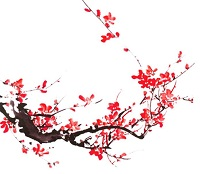
\includegraphics[keepaspectratio=true,scale=0.7, angle=90]{flower.jpg}}%
    %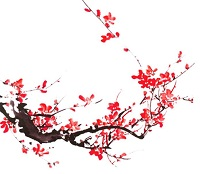
\includegraphics[keepaspectratio=true,scale=0.7, angle = -90]{flower.jpg}%
    \end{figure}%
}
  
\newcommand{\insertauthorlogo}{\vspace{-1.25\baselineskip}%    
    \begin{figure}[H]%
    \hspace*{10.10cm}%
    
\includegraphics[keepaspectratio=true,scale=0.05, angle=90]{qrcode.png}%
    \end{figure}%
}
  
\title{\Huge{\titlename}}
%\author{蘭陵笑笑生原著\\\kaishu{校對排版:細雨如煙}\\\kaishu{簡繁校對:老而彌堅劉仁軌}}
\author{會校本\quad{重訂版}\\\kaishu{蘭陵笑笑生\quad{著}}}
%\author{\kaishu{會校本{\quad{重訂版}}\\蘭陵笑笑生 著}}
\date{}

\newcommand\mydot[1]{\color{lightgray}\scalebox{#1}{.}}
\renewcommand\cftdot{\mydot{1.5}}
\renewcommand\cftdotsep{2}
%\renewcommand\cftpartnumwidth{6em}
\renewcommand{\cftchapleader}{\hspace{0.2em}{\cftdotfill{\cftdotsep}}}
%\renewcommand{\cftpnumalign}{l}

%control the right margin of toc-dots:
\makeatletter
\def\@pnumwidth{3.2em}
\makeatother

\begin{document}
\maketitle

\pagestyle{headings}
\pagenumbering{zhdig}

\pdfbookmark{書名頁}{}
\pdfbookmark{封面}{}

\includepdf[pages={1},fitpaper=false]{cover.pdf}

\cleardoublepage
\tableofcontentslocal
\pdfbookmark{\contentsname}{toc}
%prevent the 1st page of TOC generate foot page number:
\addtocontents{toc}{\protect\thispagestyle{empty}}
\mainmatter

\pagenumbering{zhdig}
\chapter*{前言}
\addcontentsline{toc}{chapter}{王汝梅《新刻繡像批評金瓶梅》前言}
\markboth{\titlename}{前言}

\begin{declareqianyan}
王汝梅\qquad\ 
\end{declareqianyan}	

《金瓶梅》是我國小說史上第一部文人獨立創作的長篇白話世情小說,對後世的小說創作與文化嬗變產生過較大影響,在文學史、文化史上具有重要地位。近年來,我國《金瓶梅》研究不斷取得新的進展,引起國外漢學家的注意。人民文學出版社出版的《金瓶梅詞話》刪節本,齊魯書社出版的《張竹坡批評第一奇書金瓶梅》刪節本,香港星海文化出版有限公司出版的《金瓶梅詞話》全校本,都促進了《金瓶梅》研究的深入發展。

《金瓶梅》的版本,大體上可分為兩個系統,三種型別。一是詞話本系統,即《新刻金瓶梅詞話》,現存三部完整刻本及一部二十三回殘本(北京圖書館藏本、日本日光山輪王寺慈眼堂藏本、日本德山毛利氏栖息堂藏本及日本京都大學附屬圖書館藏殘本)。二是崇禎本系統,即《新刻繡像批評金瓶梅》,現存約十五部(包括殘本、抄本、混合本)。第三種型別是張評本,即《張竹坡批評第一奇書金瓶梅》,屬崇禎本系統,又與崇禎本不同。在兩系三類中,崇禎本處於《金瓶梅》版本流變的中間環節。它據詞話本改寫而成,又是張評本據以改易、評點的祖本,承上啟下,至關重要。現存的崇禎本都十分珍貴,一般不易見到,因此,把存世的主要崇禎本全面地校勘一下,出版一部會校本《新刻繡像批評金瓶梅》,就顯得十分重要了。它不僅有助於認識《金瓶梅》的版本系統,而且也是探討《金瓶梅》成書之謎、作者之謎,研究作品思想藝術價值的客觀依據,是《金瓶梅》研究的基礎工程。

\subsection*{一 崇禎諸本的特徵、類別及相互關係}

刊刻於十卷本《金瓶梅詞話》之後的《新刻繡像批評金瓶梅》,是二十卷一百回本。卷首有東吳弄珠客《金瓶梅序》。書中有插圖二百幅,有的圖上題有刻工姓名,如劉應祖、劉啟先、黃子立、黃汝耀等。這些刻工活躍在天啟、崇禎年間,是新安(今安徽歙縣)木刻名手。這種刻本避明崇禎帝朱由檢諱。根據以上特點和刻本的版式字型,一般認為這種本子刻印在崇禎年間,因此簡稱為崇禎本,又稱繡像本或評改本。

現仍存世的崇禎本(包括清初翻刻的崇禎系統版本)有十幾部,各部之間大同略有小異。從版式上可分為兩大類。一類以北京大學圖書館藏本為代表,書每半葉十行,行二十二字,扉頁失去,無廿公跋,回首詩詞前有「詩曰」或「詞曰」二字。日本天理圖書館藏本、上海圖書館藏甲乙兩本、天津圖書館藏本、殘存四十七回本等,均屬此類。另一類以日本內閣文庫藏本為代表,書每半葉十一行,行二十八字,有扉頁,扉頁上題《新鐫繡像批評原本金瓶梅》,有廿公跋,回首詩詞前多無 「詩曰」或「詞曰」二字。首都圖書館藏本、日本京都大學東洋文化研究所藏本屬於此類。

崇禎諸本多有眉批和夾批。各本眉批刻印行款不同。北大本、上圖甲本以四字一行居多,也有少量二字一行的。天圖本、上圖乙本以二字一行居多,偶有四字一行和三字一行的。內閣本眉批三字一行。首圖本有夾批無眉批。

為了清理崇禎諸刻本之間的關係,需要先對幾種稀見版本作一簡單介紹:

{\large\kaishu{王孝慈舊藏本}}。王孝慈為書畫家,通縣人,原藏《新刻繡像批評金瓶梅》插圖二冊,二百幅。一九三三年北平古佚小說刊行會版詞話本中的插圖,即據王氏藏本影印。圖甚精致,署刻工姓名者多。第一回第二幅圖「武二郎冷遇親哥嫂」欄內右側題署「新安劉應祖鐫」六字,為現存其他崇禎本插圖所無。其第一回回目「西門慶熱結十弟兄」,現存多數本子與之相同,僅天圖本、上圖乙本略異。從插圖和回目判斷,王氏藏本可能是崇禎系統的原刻本。

{\large\kaishu{殘存四十七回本}}。近年新發現的。扉頁右上題「新鐫繡像批評原本」,中間大字「金瓶梅」,左題「本衙藏版」。插圖有九十幅,第五回「飲鴆藥武大遭殃」及第二十二回「蕙蓮兒偷期蒙愛」,俱題署刻工劉啟先姓名。此殘本版式、眉批行款與北大本相近,卷題也與北大本相同,但扉頁則依內閣本所謂「原本」扉頁格式刻印。此版本兼有兩類本子的特徵,是較晚出的版本,大約刊印在張評本刻印前的順治或康熙初年,流傳至張評本刊印之後。該書流傳中失去五十三回,用張評本配補,成了崇禎本和張評本的混合本。從明末至清中葉,《金瓶梅》由詞話本、崇禎本同步流傳演變為崇禎本和張評本同步流傳,其遞變端倪,可由此本看出。

{\large\kaishu{吳曉鈴先生藏抄本}}。四函四十冊,二十卷百回,是一部書品闊大的烏絲欄大字抄本。抄者為抄本刻制了四方邊欄、行間夾線和書口標「金瓶梅」的木版。吳先生云:「從字型風格看來,應屬乾隆前期。」書中穢語刪除,無眉批夾批。在崇禎諸本的異文處,此本多與北大本相同,但也有個別地方與北大本不同。由此看來,此本可能系據崇禎系統原刊本抄錄,在研究崇禎本流變及版本校勘上,頗有價值。

{\large\kaishu{《繡刻古本八才子詞話》}}。吳曉鈴先生云:「順治間坊刻《繡像八才子詞話》,大興傅氏碧蕖館舊藏。今不悉散佚何許。」(《金瓶梅詞話最初刊本問題》)吳先生把此一種本子視為清代坊間刊詞話本。美國韓南教授着錄:「扉頁題《繡刻古本八才子詞話》,其下有『本衙藏版』等字。現存五冊:序文一篇、目錄,第一、二回,第十一至十五回,第三十一至三十五回,第六十五至六十八回。序文年代順治二年(一六四五),序者不詳。十卷百回。無插圖。」(《金瓶梅的版本及其他》)韓南把它列入崇禎本系統。因韓南曾借閱傅惜華藏書,筆者採取韓南的意見,把此版本列入崇禎系統。

{\large\kaishu{周越然舊藏本}}。周越然着錄:「新刻繡像批評金瓶梅二十卷百回。明崇禎間刊本,白口,不用上下魚尾,四周單欄,每半頁十行,每行二十二字,眉上有批評,行間有圈點。卷首有東吳弄珠客序三葉,目錄十葉,精圖一百葉。此書版刻、文字均佳。」據版式特徵應屬北大本一類,與天圖本、上圖乙本相近或同版。把現存周越然舊藏本第二回圖「俏潘娘簾下勾情」影印件與北大本圖對勘,北大本圖左下有 「黃子立刊」四字,周藏本無(右下有周越然章)。

根據上述稀見版本的着錄情況和對現存崇禎諸本的考查,我們大體上可以判定,崇禎系統內部各本之間的關係是這樣的:目前僅存插圖的通州王氏舊藏本為原刊本或原版後印本。北大本是以原刊本為底本翻刻的,為現存較完整的崇禎本。以北大本為底本翻刻或再翻刻,產生出天理本、天圖本、上圖甲乙本、周越然舊藏本。對北大本一類版本稍作改動並重新刊印的,有內閣本、東洋文化研究所本、首圖本。後一類版本卷題作了統一,正文文字有改動,所改之處,多數是恢復了詞話本原字詞。在上述兩類崇禎本流傳之後,又刊刻了殘存四十七回本,此本兼有兩類版本的特徵。為使讀者一目了然,特將所知見諸本關係,列表如下:
{\clearpage}
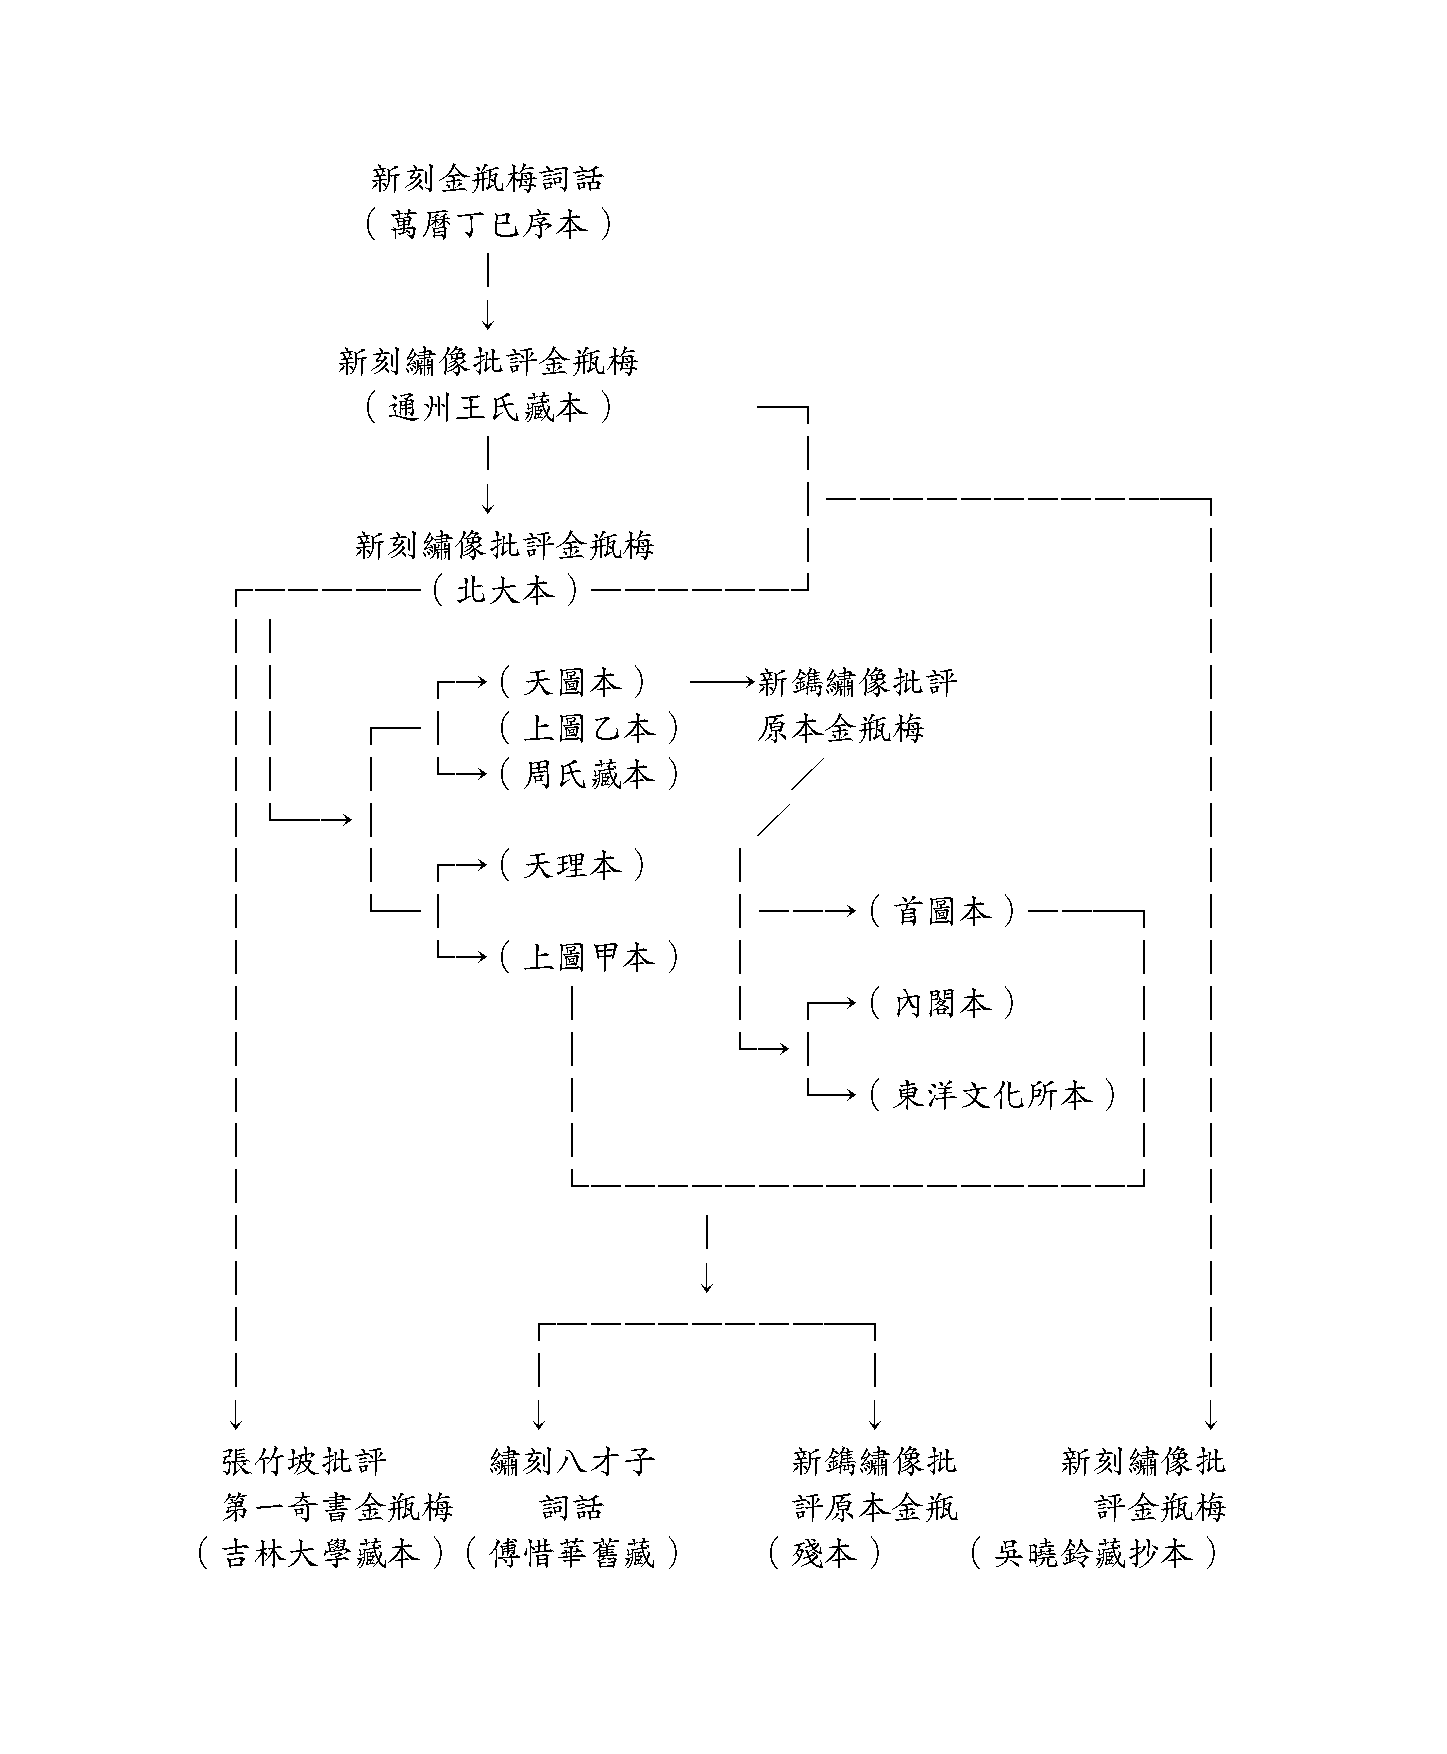
\includepdf[pages={1},fitpaper=false]{version_relations.pdf}

\subsection*{二、崇禎本和萬曆詞話本的關係}

崇禎本與萬曆詞話本相同又相異,相異而又相關。茲就崇禎本與萬曆詞話本明顯的相異之處,考查一下二者之間的關係。

(一)改寫第一回及不收欣欣子序。崇禎本把第一回「景陽岡武松打虎」改為「 西門慶熱結十弟兄」。從開首到「知縣陞堂,武松下馬進去」,是改寫者手筆,以 「財色」論作引子,寫至十弟兄在玉皇廟結拜。文句中有「打選衣帽光鮮」、「看飯來」、「哥子」、「千百斤水牛般氣力」等江浙習慣用語。「武松下馬進去」以後,文字大體與詞話本同,刪減了「看顧」、「叉兒難」等詞語。改寫後,西門慶先出場,然後是潘金蓮嫌夫賣風月,把原來武松為主、潘金蓮為賓,改成了西門慶、潘金蓮為主、武松為賓。改寫者對《金瓶梅》有自己的看法,他反對欣欣子的觀點,因此把詞話本中與欣欣子序思想一致的四季詞、四貪詞、引子,統統刪去了。

欣欣子序闡述了三個重要觀點:第一、《金瓶梅傳》作者是「寄意於時俗,蓋有謂也。」第二、《金瓶梅傳》是發憤之作,作者「爰罄平日所蘊者,着斯傳」。第三、《金瓶梅傳》雖「語涉俚俗,氣含脂粉」,但不是淫書。欣欣子冲破儒家詩教傳統,提出不要壓抑哀樂之情的進步觀點。他說:「富與貴,人之所慕也,鮮有不至於淫者;哀與怨,人之所惡也,鮮有不至於傷者。」這種觀點與李贄反對「矯強」、主張「自然發於性情」的反禮教思想是一致的。崇禎本改寫者反對這種觀點,想用「財色」論、「懲戒」說再造《金瓶梅》,因此他不收欣欣子序。而東吳弄珠客序因觀點與改寫者合拍,遂被刊為崇禎本卷首。

(二)改寫第五十三、五十四回。崇禎本第五十三、五十四兩回,與詞話本大異小同。詞話本第五十三回「吳月娘承歡求子息,李瓶兒酬願保官哥」,把月娘求子息和瓶兒保官哥兩事聯絡起來,圍遶西門慶「子嗣」這一中心展開情節,中間穿插潘金蓮與陳經濟行淫、應伯爵為李三、黃四借銀。崇禎本第五十三回「潘金蓮驚散幽歡,吳月娘拜求子息」,把潘金蓮與陳敬濟行淫描寫加濃,並標為回目,把李瓶兒酬願保官哥的情節作了大幅度刪減。改寫者可能認為西門慶不信鬼神,所以把灼龜、劉婆子收驚、錢痰火拜佛、西門慶謝土地、陳經濟送紙馬等文字都刪去了。崇禎本第五十四回把詞話本劉太監庄上河邊郊園會諸友,改為內相陸地花園會諸友,把瓶兒胃虛血少之病,改為下淋不止之病。瓶兒死於血山崩,改寫者可能認為血少之症與結局不相符而改。上述兩回,儘管文字差異較大,內容亦有增有減,但基本情節並沒有改變,仍可以看出崇禎本是據萬曆詞話本改寫而成,並非另有一種底本。

值得注意的是,詞話本第五十三、五十四兩回與前後文脈絡貫通,風格也較一致,而崇禎本這兩回卻描寫粗疏,與前後文風格亦不太一致。例如讓應伯爵當西門慶面說:「只大爹他是有名的潘驢鄧小閑不少一件」,讓陳敬濟偷情時扯斷潘金蓮褲帶,都顯然不符合人物性格,手法拙劣。

(三)崇禎諸本均避崇禎皇帝朱由檢諱,詞話本不避。如詞話本第十七回「則虜患何由而至哉!」、「皆由京之不職也」,崇禎本改「由」為「繇」;第九十五回 「巡檢司」、「吳巡檢」,崇禎本改「檢」為「簡」。此一現象亦說明崇禎本刊刻在後,並系據詞話本而改。

(四)崇禎本在版刻上保留了詞話本的殘存因素。北大本第九卷題作「新刻繡像批點金瓶梅詞話卷之七」,這是崇禎本據詞話本改寫的直接證明。此外,詞話本誤刻之字,崇禎本亦徃徃相沿而誤。如詞話本第五十七回:「我前日因徃西京」,「 西京」為「東京」之誤刻,崇禎本相沿;詞話本第三十九回:「老爹有甚釣語分付 」,「釣」為「鈞」之誤刻,北大本、內閣本亦相沿。上述殘存因素,可以看作是崇禎本與其母體《新刻金瓶梅詞話》之間的臍帶。

(五)其他相異之處:崇禎本刪去詞話本第八十四回吳月娘為宋江所救一段文字;崇禎本改動詞話本中部分情節;崇禎本刪去詞話本中大量詞曲;崇禎本刪減或改動了詞話本中的方言語詞;崇禎本改換了詞話本的回首詩詞;崇禎本比詞話本回目對仗工整;等等。

大量版本資料說明,崇禎本是以萬曆詞話本為底本進行改寫的,詞話本刊印在前,崇禎本刊印在後。崇禎本與詞話本是母子關係,而不是兄弟關係。

崇禎本刊印前,也經過一段傳抄時間。謝肇淛就提到二十卷抄本問題。他在《金瓶梅跋》中說:「書凡數百萬言,為卷二十,始末不過數年事耳。」這篇跋,一般認為寫於萬曆四十四年至四十六年(一六一六——一六一八)。這時謝肇淛看到的是不全的抄本,於袁宏道得其十三,於丘諸城得其十五。看到不全抄本,又云「為卷二十」,說明謝已見到回次目錄。二十卷本目錄是分卷次排列的。這種抄本是崇禎本的前身。設計刊刻十卷詞話本與籌劃改寫二十卷本,大約是同步進行的。可能在刊印詞話本之時即進行改寫,在詞話本刊印之後,以刊印的詞話本為底本完成改寫本定稿工作,於崇禎初年刊印《新刻繡像批評金瓶梅》。繡像評改本的改寫比我們原來想象的時間要早些。但是,崇禎本稿本也不會早過十卷本的定型本。蒲安迪教授認為,崇禎本的成書時間應「提前到小說最早流傳的朦朧歲月中,也許甚至追溯到小說的寫作年代」(《論崇禎本金瓶梅的評註》),顯然是不妥當的。從崇禎本的種種特徵來看,它不可能與其母本詞話本同時,更不可能早於母本而出生。

\subsection*{三 崇禎本評語在小說批評史上的重要地位}

崇禎本評語是古代小說批評的一宗珍貴遺產。評點者在長篇小說由英雄傳奇向世情小說蛻變的轉折時期,冲破傳統觀念,在李贄、袁宏道的「童心」、「性靈」 、「真趣」、「自然」的審美新意識啟示下,對《金瓶梅》藝術成就進行了開拓性的評析。評點者開始注重寫實,注重人物性格心理的品鑑,在馮夢龍、金聖嘆、李漁、張竹坡、脂硯齋之前,達到了古代小說批評的新高度。其主要價值有如下幾點:

(一)肯定《金瓶梅》是一部世情書,而非淫書。評點者認為書中所寫人事天理,全為「世情所有」,「如天造地設」。評點者第一次把《金瓶梅》與《史記》相提並論,認為《金瓶梅》「從太史公筆法來」,「純是史遷之妙」。評點者批判了淫書論,他說:「讀此書而以為淫者、穢者,無目者也。」明末《金瓶梅》評論有三派觀點。第一,從進步文藝思潮出發,對《金瓶梅》的產生表示驚喜、贊賞,以欣欣子、袁宏道、謝肇淛為代表。第二,接受進步思潮影響,又受傳統觀念束縛,對此書持又肯定又否定態度,認為此書是淫書、穢書,所以要刊印,蓋為世戒,非為世勸,以東吳弄珠客為代表。第三,固守傳統觀念,持全盤否定看法,認為此書淫穢,壞人心術,決當焚之,以董思白為代表。崇禎本評點者鮮明地批評了第二、第三兩種觀點。

(二)分析了《金瓶梅》中衆多人物的複雜性格。魯迅曾指出,《紅樓夢》的可貴之處在於它突破了我國小說人物塑造中「叙好人完全是好,壞人完全是壞」的傳統格局。其實,最早突破這一格局的應該是《金瓶梅》。《金瓶梅》已經擺脫了傳統小說那種簡單化的平面描寫,開始展現真實的人所具有的複雜矛盾的性格。對於這一點,崇禎本評點者注意到了。他在評析潘金蓮時,既指出她的「出語狠辣」 ,「俏心毒口」,慣於「聽籬察壁」、「愛小便宜」等弱點,也贊美她的「慧心巧舌」、「韻趣動人」等「可愛」之處。評析李瓶兒時,既說她「愚」、「淺」,也指出她「醇厚」、「情深」。即使是西門慶,評點者亦認為作者並非把他寫得絕對的惡,指出「西門慶臨財徃徃有廉恥、有良心」,資助朋友時「脫手相贈,全無吝色」。尤其可貴的是,評點者冲破了封建傳統道德的束縛,對潘金蓮這樣一個「淫婦」,處處流露出贊美和同情。在潘金蓮被殺後,評點者道:「讀至此,不敢生悲,不忍稱快,然而心實惻惻難言哉!」這是對一個複雜形象的充滿矛盾的審美感受。

(三)評析了作者刻畫人物的傳神技巧。評點者說作者「寫笑則有聲,寫想則有形」,「並聲影、氣味、心思、胎骨」俱摹出,「真爐錘造物之手」。他特別贊賞對潘金蓮的刻畫,說其「撒嬌弄癡,事事堪入畫」,其「靈心利口」,「乖恬」 「可愛」。在四十三回作者寫金蓮喬粧假哭時,評點者道:「倔強中實含軟媚,認真處微帶戲謔」,點出作者不僅善於描摹人物的聲容笑貌,還能借形傳神,展現人物的內心世界。

(四)崇禎本評語顯示了評點者新的藝術視角。傳統的評論重教化而不重審美,重史實而不重真趣。評點者冲破這種傳統,從新的藝術視角對《金瓶梅》全面品評。他稱作者為「寫生手」,很多評語肯定作品的寫實特點,白描手法,一再評述作者的藝術真趣。通俗、真趣、寫生,這種新和藝術視角,反映了萬曆中後期的美學追求。馮夢龍的「事贗而理真」論,金聖嘆的性格論,李漁的幻境論,張竹坡的情理論,脂硯齋的「情情」論,使古代小說批評達到成熟與繁榮的高峰,而早於他們的崇禎本評點者,對明清小說批評的發展,可以說起了奠基與開拓的作用。

袁宏道在一六九五年傳遞了《金瓶梅》抄本的第一個資訊,驚訝《金瓶梅》的出現,肯定《金瓶梅》的自然之美。謝肇淛在《金瓶梅跋》中稱此書為「稗官之上乘」,作者為「爐錘之妙手」,特別評述了作者寫人物「不徒俏其貌,且並其神傳之」的特點。崇禎本評點,可以看作是袁宏道、謝肇淛對《金瓶梅》評價具體化的審美反映。



\chapter*{金瓶梅序}
\addcontentsline{toc}{chapter}{東吴弄珠客《金瓶梅序》}
\markboth{\titlename}{金瓶梅序}


《金瓶梅》,穢書也。袁石公亟稱之,亦自寄其牢騷耳,非有取於《金瓶梅》也。然作者亦自有意,蓋為世戒,非為世勸也。如諸婦多矣,而獨以潘金蓮、李瓶兒、春梅命名者,亦楚《檮杌》之意也。蓋金蓮以奸死,瓶兒以孽死,春梅以淫死,較諸婦為更慘耳。借西門慶以描畫世之大淨,應伯爵以描繪世之小丑,諸淫婦以描畫世之醜婆、淨婆,令人讀之汗下。蓋為世戒,非為世勸也。余嘗曰:「讀《金瓶梅》而生憐憫心者,菩薩也;生畏懼心者,君子也;生歡喜心者,小人也;生效法心者,乃禽獸耳。」余友人褚孝秀偕一少年同赴歌舞之筵,衍至霸王夜宴,少年垂涎曰:「男兒何可不如此!」褚孝秀曰:「也只為這烏江設此一着耳。」同座聞之,嘆為有道之言。若有人識得此意,方許他讀《金瓶梅》也。不然,石公幾為導淫宣慾之尤矣。奉勸世人,勿為西門之後車可也。

\begin{quotation}
\raggedleft{東吳弄珠客題\rightquadmargin}
\end{quotation}


\chapter*{金瓶梅詞話序}
\addcontentsline{toc}{chapter}{欣欣子《金瓶梅詞話序》}
\markboth{\titlename}{金瓶梅詞話序}


竊謂蘭陵笑笑生作《金瓶梅傳》,寄意於時俗,蓋有謂也。人有七情,憂鬱為甚。上智之士,與化俱生,霧散而冰裂,是故不必言矣。次焉者,亦知以理自排,不使為累。惟下焉者,既不能了於心胸,又無詩書道腴可以撥遣,然則不致於坐病者幾希!吾友笑笑生為此,爰罄平日所蘊者,著斯傳,凡一百囬。其中語句新奇,膾炙人口。無非明人倫、戒淫奔、分淑慝、化善惡,知盛衰消長之機,取報應輪迴之事,如在目前;始終如脈絡貫通,如萬絲迎風而不亂也。使觀者庶幾可以一哂而忘憂也。其中未免語涉俚俗,氣含脂粉。余則曰:不然。《關雎》之作,楽而不淫,哀而不傷。富與貴,人之所慕也,鮮有不至於淫者;哀與怨,人之所惡也,鮮有不至於傷者。吾嘗觀前代騷人,如盧景暉之《剪燈新話》、元微之之《鶯鶯傳》、趙君弼之《效顰集》、羅貫中之《水滸傳》、丘瓊山之《鍾情麗集》、盧梅湖之《懷春雅集》、周靜軒之《秉燭清談》,其後《如意傳》、《于湖記》,其間語句文確,讀者往往不能暢懷,不至終篇而掩棄之矣。此一傳者,雖市井之常談,閨房之碎語,使三尺童子聞之,如飫天漿而拔鯨牙,洞洞然易曉。雖不比古之集理趣,文墨綽有可觀。其它關繋世道風化,懲戒善惡,滌慮洗心,不無小補。譬如房中之事,人皆好之,人非堯舜聖賢,鮮不為所耽。富貴善良,人皆惡之,是以搖動人心,蕩其素志。觀其高堂大廈,雲窗霧閣,何深沉也;金屏繡褥,何羙麗也;鬢雲斜軃,春酥滿胸,何嬋娟也;雄鳳雌凰迭舞,何慇懃也;錦衣玉食,何侈費也;佳人才子,嘲風咏月,何綢繆也;鷄舌含香,唾圓流玉,何溢度也;一雙玉腕綰復綰,兩隻金蓮顛倒顛,何猛浪也。旣其樂矣,然楽極必悲生:如離别之機將興,憔悴之容必見者,所不能免也;折梅逢驛使,尺素寄魚書,所不能無也;患難迫切之中,顛沛流離之頃,所不能脫也;陷命於刀劍,所不能逃也;陽有王灋,幽有鬼神,所不能逭也。至於淫人妻子,妻子淫人,祸因惡積,福緣善慶,種種皆不出循環之機。故天有春夏秋冬,人有悲歡離合,莫怪其然也。合天時者,遠則子孫悠久,近則安享終身;逆天時者,身名罹喪,祸不旋踵。人之䖏世,雖不出乎世運代謝,然不經凶祸,不蒙耻辱者,亦幸矣。吾故曰:笑笑生作此傳者,蓋有所謂也。

\begin{quotation}
\raggedleft{欣欣子書於明賢里之軒\rightquadmargin}
\end{quotation}


\chapter*{跋}
\addcontentsline{toc}{chapter}{廿公《跋》}
\markboth{\titlename}{跋}


《金瓶梅》,傳為世廟時一鉅公寓言,蓋有所刺也。然曲盡人間醜態,其亦先師不删鄭衛之旨乎?中間䖏處埋伏因果,作者亦大慈悲矣。今後流行此書,功德無量矣。不知者竟目為淫書,不惟不知作者之旨,併亦寃卻流行者之心矣!特為白之。

\begin{quotation}
\raggedleft{廿公書\rightquadmargin}
\end{quotation}


\chapter*{謝肇淛《金瓶梅》跋}
\addcontentsline{toc}{chapter}{謝肇淛《金瓶梅》跋}
\markboth{\titlename}{謝肇淛《金瓶梅》跋}

《金瓶梅》一書,不著作者名代。相傳永陵中有金吾戚裡,憑怙奢汰,淫縱無度,而其門客病之,採摭日逐行事,匯以成編,而托之西門慶也。書凡數百萬言,為卷二十,始末不過數年事耳。

其中朝野之政務,官私之晉接,閨闥之蝶語,市裡之猥談,與夫勢交利合之態,心輸背笑之局,桑中濮上之期,尊罍枕席之語,駔驗之機械意智,粉黛之自媚爭妍,狎客之從臾逢迎,奴怡之嵇唇淬語,窮極境像,駥意快心。譬之范工摶泥,妍媸老少,人鬼萬殊,不徒肖其貌,且並其神傳之。信稗官之上乘,爐錘之妙手也。其不及《水滸傳》者,以其猥瑣淫蝶,無關名理。而或以為過之者,彼猶機軸相放,而此之面目各別,聚有自來,散有自去,讀者竟想不到,唯恐易盡。此豈可與褒儒俗士見哉。此書向無鏤版,抄寫流傳,參差散失。唯弇州家藏者最為完好。余於袁中郎得其十三,於丘諸城得其十五,稍為釐正,而闕所未備,以俟他日。有嗤余誨淫者,余不敢知。然溱洧之音,聖人不刪,則亦中郎帳中必不可無之物也。仿此者有《玉嬌麗》,然而乖彞敗度,君子無取焉。
  
\begin{quotation}\begin{flushright}謝肇淛。\end{flushright}\end{quotation}


\chapter*{新鐫金瓶梅詞話}
\addcontentsline{toc}{chapter}{新刻金瓶梅詞話·詞曰·四貪詞}
\markboth{\titlename}{新刻金瓶梅詞話·詞曰·四貪詞}


\section*{詞曰}

\begin{myquote0}
閬苑瀛洲,金谷瓊樓,算不如茅舍清幽。野花繡地,莫也風流。也宜春,也宜夏,也宜龝。

酒熟堪あ,客至須留,更無榮無辱無憂。退閒一步,着甚來由。但倦時眠,渴時飲,醉時謳。

短短横牆,矮矮疎窗,忔い兒小小池塘。高低疊嶂,綠水邊傍。也有些風,有些月,有些凉。

日用家常,竹几藤牀,據眼前水色山光。客來無酒,清話何妨。但細烹茶,熱烘盞,淺澆湯。

水竹之居,吾愛吾盧,石磷磷粧砌階除。軒窗隨意,小巧規模。却也清幽,也瀟灑,也寬舒。

懶散無拘,此等何如:倚闌干臨水觀魚。風花雪月,贏得功夫,好炷些香,說些話,讀些書。

淨掃塵埃,惜取蒼苔,任門前紅葉鋪階。也堪圖畫,還也奇哉。有數株松,數杆竹,數枝梅。

花木栽培,取次教開,明朝事天自安排。知他富貴幾時來。且優遊,且隨分,且開懷。
\end{myquote0}

\newpage\section*{四貪詞}
%\addcontentsline{toc}{chapter}{四貪詞}
%\markboth{\titlename}{四貪詞}

\hspace*{1em}酒

\begin{myquote0}
酒損精神破喪家,語言無狀鬧喧嘩。疎親慢友多由你,背義忘恩盡是他。

切須戒,飲流霞。若能依此寳無差。失却萬事皆因此,今後逢賓只待茶。
\end{myquote0}

\hspace*{1em}色

\begin{myquote0}
休愛綠髩羙朱顔,少貪紅粉翠花鈿。損身害命多嬌態,傾國傾城色更鮮。

莫戀此,養丹田。人能寡慾壽長年。従今罷却閒風月,紙帳梅花獨自眠。
\end{myquote0}

\hspace*{1em}財

\begin{myquote0}
錢帛金珠籠内收,若非公道少貪求。親朋道義因財失,父子懷情為利休。

急縮手,且抽頭。免使身心晝夜愁。兒孫自有兒孫福,莫與兒孫作遠憂。
\end{myquote0}

\hspace*{1em}氣

\begin{myquote0}
莫使強梁逞技能,揎拳裸袖弄精神。一時怒發無明火,到後憂煎祸及身。

莫太過,免災迍。勸君凡事放寬情。合撒手時須撒手,得饒人處且饒人。
\end{myquote0}



\part*{{\titlename}卷之一}
\addcontentsline{toc}{part}{{\titlename}卷之一}


\includepdf[pages={1,2},fitpaper=false]{tst.pdf}
\chapter*{第一囘 西門慶熱結十弟兄 武二郎冷遇親哥嫂}
\addcontentsline{toc}{chapter}{第一囘 西門慶熱結十弟兄 武二郎冷遇親哥嫂}
\markboth{{\titlename}卷之一}{第一囘 西門慶熱結十弟兄 武二郎冷遇親哥嫂}


詩曰:

\begin{myquote}
豪華去後行人絕,簫箏不響歌喉咽。\\
雄劍無威光彩沉,寶琴零落金星滅。\\
玉堦寂寞墜秋露,月照當時歌舞處。\\
當時歌舞人不囘,化為今日西陵灰。{\meipi{一部炎涼境況,盡此數語中。}}
\end{myquote}

又詩曰:

\begin{myquote}
二八佳人體似酥,腰間仗劍斬愚夫。{\pangpi{不是愚夫,盡是貪夫。}}\\
雖然不見人頭落,暗裡教君骨髓枯。
\end{myquote}

這一首詩,是昔年大唐國時,一箇修真練性的英雄,入聖超凡的豪傑,到後來位居紫府,名列仙班,率領上八洞群仙,救拔四部洲沉苦一位仙長,姓呂名巖,道號純陽子祖師所作。單道世上人,營營逐逐,急急巴巴,跳不出七情六慾關頭,打不破酒色財氣圈子。到頭來同歸於盡,着甚要緊!雖是如此說,只這酒色財氣四件中,唯有「財色」二者更為利害。怎見得他的利害?假如一箇人到了那窮苦的田地,受盡無限淒涼,耐盡無端懊惱,晚來摸一摸米甕,苦無隔宿之炊,早起看一看廚前,愧無半星烟火,妻子飢寒,一身凍餒,{\meipi{情景逼真,酸徠談此,能不雪涕!}}就是那粥飯尚且艱難,那討餘錢沽酒!{\pangpi{酒因財缺。}}更有一種可恨處,親朋白眼,面目寒酸,便是淩雲志氣,分外消磨,怎能勾與人爭氣!{\pangpi{氣以財弱。}}正是:

\begin{myquote}
一朝馬死黃金盡,親者如同陌路人。
\end{myquote}

到得那有錢時節,揮金買笑,一擲鉅萬。思飲酒,真箇瓊漿玉液,{\pangpi{酒需財美。}}不數那琥珀盃流;要鬪氣,錢可通神,果然是頤指氣使。{\pangpi{氣用財伸。}}趨炎的壓脊挨肩,附勢的吮癰舐痔,真所謂得勢疊肩而來,失勢掉臂而去。古今炎冷惡態,莫有甚於此者。這兩等人,豈不是受那財的利害處!如今再說那色的利害。{\meipi{引起三段,格法一變,更見靈活。}}請看如今世界,你說那坐懷不亂的桺下惠,閉門不納的魯男子,與那秉燭達旦的關雲長,古今能有幾人?至如三妻四妾,買笑追歡的,又當別論。還有那一種好色的人,見了箇婦女畧有幾分顏色,便百計千方偷寒送暖,一到了着手時節,只圖那一瞬歡娛,也全不顧親戚的名分,也不想朋友的交情。起初時,不知用了多少濫錢,費了幾遭酒食。{\pangpi{酒。}}正是:

\begin{myquote}
三盃花作合,兩盞色媒人。
\end{myquote}

到後來情濃事露,甚而鬪狠殺傷,{\pangpi{氣。}}性命不保,妻孥難顧,事業成灰。就如那石季倫潑天豪富,為綠珠命䘮囹圄;楚霸王氣概拔山,因虞姬頭懸垓下。真說謂「生我之門死我戶,看得破時忍不過」。這樣人,豈不是受那色的利害處?說便如此說,這「財色」二字,從來只沒有看得破的。{\meipi{說的世情氷冷,須從蒲團面壁十年纔辨。}}若有那看得破的,便見得堆金積玉,是棺材內帶不去的瓦礫泥沙;貫朽粟紅,是皮囊內裝不盡的臭淤糞土。高堂廣廈,玉宇瓊樓,是墳山上起不得的享堂;錦衣繡襖,狐服貂裘,是骷髏上裹不了的敗絮。即如那妖姬艷女,獻媚工妍,看得破的,卻如交鋒陣上將軍叱吒獻威風;硃唇皓齒,掩袖囘眸,懂得來時,便是閻羅殿前鬼判夜叉增惡態。羅襪一彎,金蓮三寸,是砌墳時破土的鍬鋤;{\pangpi{尖穎異常。}}枕上綢繆,被中恩愛,是五殿下油鍋中生活。只有那《金剛經》上兩句說得好,他說道:「如夢幻泡影,如電覆如露。」見得人生在世,一件也少不得,到了那結束時,一件也用不着。隨着你舉鼎盪舟的神力,到頭來少不得骨軟觔麻;繇着你銅山金谷的奢華,正好時卻又要氷消雪散。假饒你閉月羞花的容貌,一到了垂眉落眼,人皆掩鼻而過之;比如你陸賈、隋何的機鋒,若遇着齒冷唇寒,吾末如之何也已。{\meipi{生公說法,石應肯首。}}到不如削去六根清淨,{\pangpi{伏脈。}}披上一領袈裟,叅透了空色世界,打磨穿生滅機關,直超無上乘,不落是非窠,倒得箇清閉自在,不向火坑中翻觔斗也。正是:

\begin{myquote}
三寸氣在千般用,一日無常萬事休。
\end{myquote}

說話的,為何說此一段酒色財氣的緣故?只為當時有一箇人家,先前恁地富貴,到後來煞甚淒涼,權謀術智,一毫也用不着,親友兄弟,一箇也靠不着,享不過幾年的榮華,倒做了許多的話靶。內中又有幾箇鬪寵爭強,迎奸賣俏的,起先好不妖嬈嫵媚,到後來也免不得屍橫燈影,血染空房。正是:

\begin{myquote}
善有善報,惡有惡報;天網恢恢,疏而不漏。
\end{myquote}

話說大宋徽宗皇帝政和年間,山東省東平府清河縣中,有一箇風流子弟,生得狀貌魁梧,性情瀟灑,饒有幾貫家資,年紀二十六七。這人覆姓西門,單諱一箇慶字。他父親西門達,原走川廣販藥材,就在這清河縣前開着一箇大大的生藥鋪。現住着門面五間到底七進的房子。家中呼奴使婢,騾馬成群,雖算不得十分富貴,卻也是清河縣中一箇殷實的人家。只為這西門達員外夫婦去世的早,單生這箇兒子,卻又百般愛惜,聽其所為,所以這人不甚讀書,{\pangpi{四字是一生病痛。}}終日閑遊浪蕩。一自父母亡後,專一在外眠花宿桺,惹草招風,學得些好拳棒,又會賭博,雙陸、象棋、抹牌、道字,無不通曉。結識的朋友,也都是些幫閑抹嘴,不守本分的人。第一箇最相契的,姓應名伯爵,表字光侯,原是開紬段鋪應員外的第二箇兒子,落了本錢,跌落下來,專在本司三院幫嫖貼食,因此人都起他一箇渾名,叫做應花子。又會一腿好氣毬,雙陸、棋子,件件皆通。{\meipi{叙得錯綜變化。}}第二箇姓謝名希大,字子純,乃清河衛千戶官兒應襲子孫,自幼父母雙亡,遊手好閑,把前程丟了,亦是幫閑勤兒,會一手好琵琶。自這兩箇與西門慶甚合得來。其餘還有幾箇,都是些破落戶,沒名器的。一箇叫做祝實念,表字貢誠。一箇叫做孫天化,表字伯修,綽號孫寡嘴。一箇叫做吳典恩,乃是本縣陰陽生,因事革退,專一在縣前與官吏保債,以此與西門慶徃來。還有一箇雲叅將的兄弟叫做雲理守,字非去。一箇叫做常峙節,表字堅初。一箇叫做卜志道。一箇叫做白賚光,表字光湯。說這白賚光,衆人中也有道他名字取的不好聽的,他卻自己解說道:「不然我也改了,只為當初取名的時節,原是一箇門館先生,說我姓白,當初有一箇什麼故事,是白魚躍入武王舟。又說有兩句書是『周有大賚,於湯有光』,取這箇意思,所以表字就叫做光湯。我因他有這段故事,也便不改了。」{\meipi{磊落寫來,於結處獨以此段瀠洄,便覺鬚眉生動。}}說這一干共十數人,見西門慶手裡有錢,又撒漫肯使,所以都亂撮哄着他耍錢飲酒,嫖賭齊行。正是:

\begin{myquote}
把盞啣盃意氣深,兄兄弟弟抑何親。\\
一朝平地風波起,此際相交纔見心。
\end{myquote}

說話的,這等一箇人家,生出這等一箇不肖的兒子,又搭了這等一班無益有損的朋友,隨你怎的豪富也要窮了,還有甚長進的日子!卻有一箇緣故,只為這西門慶生來秉性剛強,作事機深詭譎,又放官吏債,就是那朝中高、楊、童、蔡四大奸臣,他也有門路與他浸潤。{\meipi{好針線。}}所以專在縣裡管些公事,與人把攪說事過錢,因此滿縣人都懼怕他。因他排行第一,人都叫他是西門大官人。這西門大官人先頭渾家陳氏早逝,身邊只生得一箇女兒,叫做西門大姐,就許與東京八十萬禁軍楊提督的親家陳洪的兒子陳敬濟為室,尚未過門。只為亡了渾家,無人管理家務,新近又娶了本縣清河左衛吳千戶之女,填房為繼室。這吳氏年紀二十五六,是八月十五生的,小名叫做月姐,後來嫁到西門慶家,都順口叫他月娘。卻說這月娘秉性賢能,夫主面上百依百隨。{\meipi{如此賢婦,世上有幾?}}房中也有三四箇丫鬟婦女,都是西門慶收用過的。又嘗與勾欄內李嬌兒打熱,也娶在家裡做了第二房娘子。南街又佔着窠子卓二姐,名卓丟兒,包了些時,也娶來家做了第三房。只為卓二姐身子瘦怯,時常三病四痛,他卻又去飄風戲月,調弄人家婦女。正是:

\begin{myquote}
東家歌笑醉紅顏,又向西隣開玳宴。\\
幾日碧桃花下臥,牡丹開處總堪憐。
\end{myquote}

話說西門慶一日在家閑坐,對吳月娘說道:「如今是九月廿五日了,出月初三日,卻是我兄弟們的會期。到那日也少不的要整兩席齊整的酒席,叫兩箇唱的姐兒,自恁在咱家與兄弟們好生玩耍一日。你與我料理料理。」吳月娘便道:「你也便別要說起這幹人,那一箇是那有良心和行貨!無過每日來勾使的遊魂撞屍。我看你自搭了這起人,幾時曾着箇家哩!{\meipi{數語可配名臣諫疏。}}現今卓二姐自恁不好,我勸你把那酒也少要吃了。」西門慶道:「你別的話倒也中聽。今日這些說話,我卻有些不耐煩聽他。依你說,這些兄弟們沒有好人,別的倒也罷了,自我這應二哥,這一箇人本心又好,又知趣着人,{\pangpi{溺愛者智昏,不止西門一箇。}}使着他,沒有一箇不依順的,做事又十分停當。就是那謝子純這箇人,也不失為箇伶俐能事的好人。咱如今是這等計較罷,只管恁會來會去,終不着箇切實。咱不如到了會期,都結拜了兄弟罷,明日也有箇靠傍些。」吳月娘接過來道:「結拜兄弟也好。只怕後日還是別箇靠你的多哩。若要你去靠人,提傀儡兒上戲場——還少一口氣兒哩。」西門慶笑道:「咱恁長把人靠得着,卻不更好了。咱只等應二哥來,與他說這話罷。」正說着話,只見一箇小厮兒,生得眉清目秀,伶俐乖覺,原是西門慶貼身伏侍的,喚名玳安兒,走到面前來說:「應二叔和謝大叔在外見爹說話哩。」西門慶道:「我正說他,他卻兩箇就來了。」一面走到廳上來,只見應伯爵頭上戴一頂新盔的玄羅帽兒,身上穿一件半新不舊的天青夾縐紗褶子,脚下絲鞋淨襪,坐在上首。下首坐的便是姓謝的謝希大。見西門慶出來,一齊立起身來,邊忙作揖道:「哥在家,連日少看。」西門慶讓他坐下,一面喚茶來吃,說道:「你們好人兒,這幾日我心裡不耐煩,不出來走跳,你們通不來傍箇影兒。」伯爵向希大道:「何如?我說哥要說哩。」因對西門慶道:「哥,你恠的是。連咱自也不知道成日忙些什麼!自咱們這兩隻脚,還趕不上一張嘴哩。」西門慶因問道:「你這兩日在那裡來?」伯爵道:「昨日在院中李家瞧了箇孩子兒,就是哥這邊二嫂子的姪女兒、桂卿的妹子,叫做桂姐兒。幾時兒不見他,就出落的好不標致了。到明日成人的時候,還不知怎的樣好哩!昨日他媽再三向我說:『二爹,千萬尋箇好子弟梳籠他。』敢怕明日還是哥的貨兒哩。」{\pangpi{伏脈。}}西門慶道:「有這等事!等咱空閑了去瞧瞧。」謝希大接過來道:「哥不信,委的生得十分顏色。」西門慶道:「昨日便在他家,前幾日卻在那裡去來?」伯爵道:「便是前日卜志道兄弟死了,咱在他家幫着亂了幾日,傳送他出門。{\pangpi{伏脈。}}他嫂子再三向我說,叫我拜上哥,承哥這裡送了香楮奠礼去,因他沒有寬轉地方兒,晚夕又沒甚好酒席,不好請哥坐的,甚是過不意去。」西門慶道:「便是我聞得他不好得沒多日子,就這等死了。我前日承他送我一把真金川扇兒,我正要拏甚答謝答謝,不想他又作了故人!」

謝希大便嘆了一口氣道:「咱會中兄弟十人,卻又少他一箇了。」因向伯爵說:「出月初三日,又是會期,咱每少不得又要煩大官人這裡破費,兄弟們頑耍一日哩。」西門慶便道:「正是,我剛纔正對房下說來,咱兄弟們似這等會來會去,無過只是吃酒頑耍,不着一箇切實,倒不如尋一箇寺院裡,寫上一箇疏頭,結拜做了兄弟,到後日彼此扶持,有箇傍靠。到那日,咱少不得要破些銀子,買辦三牲,衆兄弟也便隨多少各出些分資。不是我科派你們,這結拜的事,各人出些,也見些情分。」伯爵連忙道:「哥說的是。婆兒燒香當不的老子念佛,各自要儘自的心。只是俺衆人們,老鼠尾巴生瘡兒——有膿也不多。」西門慶笑道:「恠狗才,誰要你多來!你說這話。」謝希大道:「結拜須得十箇方好。如今卜志道兄弟沒了,卻教誰補?」西門慶沉吟了一囘,說道:「咱這間壁花二哥,原是花太監姪兒,手裡肯使一股濫錢,常在院中走動。他家後邊院子與咱家只隔着一層壁兒,{\pangpi{伏脈。}}與我甚說得來,咱不如叫小厮邀他邀去。」應伯爵拍着手道:「敢就是在院中包着吳銀兒的花子虛麼?」西門慶道:「正是他!」伯爵笑道:「哥,快叫那箇大官兒邀他去。{\pangpi{等不得了。}}與他徃來了,咱到日後,敢又有一箇酒碗兒。」西門慶笑道:「傻花子,你敢害饞癆痞哩,說着的是吃。」大家笑了一囘。西門慶旋叫過玳安兒來說:「你到間壁花家去,對你花二爹說,如此這般:『俺爹到了出月初三日,要結拜十兄弟,敢叫我請二爹上會哩。』看他怎的說,你就來囘我話。你二爹若不在家,就對他二娘說罷。」玳安兒應諾去了。伯爵便道:「到那日還在哥這裡是,還在寺院裡好?」希大道:「咱這裡無過只兩箇寺院,僧家便是永福寺,道家便是玉皇廟。{\pangpi{又伏永福寺、玉皇廟。}}這兩箇去處,隨分那裡去罷。」西門慶道:「這結拜的事,不是僧家管的,那寺裡和尚,我又不熟,倒不如玉皇廟吳道官與我相熟,他那裡又寬展又幽靜。」伯爵接過來道:「哥說的是,敢是永福寺和尚倒和謝家嫂子相好,故要薦與他去的。」希大笑罵道:「老花子,一件正事,說說就放出屁來了。」

正說笑間,只見玳安兒轉來了,因對西門慶說道:「他二爹不在家,俺對他二娘說來。二娘聽了,好不歡喜,{\pangpi{伏脈。}}說道:『既是你西門爹攜帶你二爹做兄弟,那有箇不來的。{\meipi{只恐攜帶二爹,便要插戴二娘。}}等來家我與他說,至期以定攛掇他來,多拜上爹。』又與了小的兩件茶食來了。」{\pangpi{閑處都韻。}}西門慶對應、謝二人道:「自這花二哥,倒好箇伶俐標致娘子兒。」{\pangpi{伏脈。}}

說畢,又拏一盞茶吃了,二人一齊起身道:「哥,別了罷,咱好去通知衆兄弟,糾他分資來。哥這裡先去與吳道官說聲。」西門慶道:「我知道了,我也不留你罷。」於是一齊送出大門來。應伯爵走了幾步,迴轉來道:「那日可要叫唱的?」西門慶道:「這也罷了,弟兄們說說笑笑,到有趣些。」說畢,伯爵舉手,和希大一路去了。

話休饒舌,撚指過了四五日,卻是十月初一日。西門慶早起,剛在月娘房裡坐的,只見一箇纔留頭的小厮兒,手裡拏着箇描金退光拜匣,走將進來,向西門慶磕了一箇頭兒,立起來站在傍邊說道:「俺是花家,俺爹多拜上西門爹。

那日西門爹這邊叫大官兒請俺爹去,俺爹有事出門了,不曾當面領教的。聞得爹這邊是初三日上會,俺爹特使小的先送這些分資來,說爹這邊胡亂先用着,等明日爹這裡用過多少派開,該俺爹多少,再補過來便了。」西門慶拏起封袋一看,簽上寫着「分資一兩」,便道:「多了,不消補的。到後日叫爹莫徃那去,起早就要同衆爹上廟去。」那小厮兒應道:「小的知道。」剛待轉身,被吳月娘喚住,{\pangpi{臨去秋波。}}叫大丫頭玉簫在食籮裡揀了兩件蒸酥菓餡兒與他。因說道:「這是與你當茶的。你到家拜上你家娘,{\pangpi{想必要結姊妹。}}你說西門大娘說,遲幾日還要請娘過去坐半日兒哩。」那小厮接了,又磕了一箇頭兒,應着去了。

西門慶纔打發花家小厮出門,只見應伯爵家應寶夾着箇拜匣,玳安兒引他進來見了,磕了頭,說道:「俺爹糾了衆爹們分資,叫小的送來,爹請收了。」西門慶取出來看,共總八封,也不拆看,都交與月娘,道:「你收了,到明日上廟,好湊着買東西。」說畢,打發應寶去了。立起身到那邊看卓二姐。剛走到坐下,只見玉簫走來,說道:「娘請爹說話哩。」{\pangpi{餘波。}}西門慶道:「怎的起先不說來?」隨即又到上房,看見月娘攤着些紙包在面前,指着笑道:「你看這些分子,止有應二的是一錢二分八成銀子,其餘也有三分的,也有五分的,都是些紅的、黃的,倒象金子一般。咱家也曾沒見這銀子來,收他的也汙箇名,不如掠還他罷。」西門慶道:「你也耐煩,丟着罷,咱多的也包補,在乎這些?」說着一直徃前去了。

到了次日初二日,西門慶稱出四兩銀子,叫家人來興兒買了一口豬、一口羊、五六罈金華酒和香燭紙劄、雞鴨案酒之物,又封了五錢銀子,旋叫了大家人來保和玳安兒、來興三箇:「送到玉皇廟去,對你吳師父說,俺爹明日結拜兄弟,要勞師父做紙疏辭,晚夕就在師父這裡散福。煩師父與俺爹預備預備,俺爹明早便來。」只見玳安兒去了一會,來囘說:「已送去了,吳師父說知道了。」

須臾,過了初二,次日初三早,西門慶起來梳洗畢,叫玳安兒:「你去請花二爹,到咱這裡吃早飯,一同好上廟去。一發到應二叔家,叫他催催衆人。」

玳安應諾去,剛請花子虛到來,只見應伯爵和一班兄弟也來了,卻正是前頭所說的這幾箇人。為頭的便是應伯爵,謝希大、孫天化、祝念實、吳典恩、雲理守、常峙節、白賚光,連西門慶、花子虛共成十箇。進門來一齊籮圈作了一箇揖。伯爵道:「咱時候好去了。」西門慶道:「也等吃了早飯着。」便叫:「拏茶來。」一面叫:「看菜兒。」須臾,吃畢早飯,西門慶換了一身衣服,打選衣帽光鮮,一齊徑徃玉皇廟來。不到數裡之遙,早望見那座廟門,造得甚是雄峻。但見:

\begin{myquote}
殿宇嵯峨,宮墻高聳。正面前,起着一座墻門八字,一帶都粉赭色紅泥;進裡邊,列着三條甬道川紋,四方都砌水痕白石。正殿上金碧輝煌,兩廊下簷阿峻峭。三清聖祖莊嚴寶相列中央,太上老君背倚青牛居後殿。
\end{myquote}

進入第二重殿後,轉過一重側門,卻是吳道官的道院。進的門來,兩下都是些瑤草琪花,蒼松翠竹。西門慶擡頭一看,只見兩邊門楹上貼着一副對聯道:

\begin{myquote}
洞府無窮歲月,壺天別有乾坤。
\end{myquote}

上面三間敞廳,卻是吳道官朝夕做作功課的所在。當日鋪設甚是齊整,上面掛的是昊天金闕玉皇上帝,兩邊列着的紫府星官,側首掛着便是馬、趙、溫、關四大元帥。{\pangpi{伏脈。}}當下吳道官卻又在經堂外躬身迎接。西門慶一起人進入裡邊,獻茶已罷,衆人都起身,四圍觀看。白賚光攜着常峙節手兒,從左邊看將過來,一到馬元帥面前,見這元帥威風凜凜,相貌堂堂,面上畫着三隻眼睛,便叫常峙節道:「哥,這卻是怎的說?如今世界,開隻眼閉隻眼兒便好,還經得多出隻眼睛看人破綻哩!」應伯爵聽見,走過來道:「呆兄弟,他多隻眼兒看你倒不好麼?」{\pangpi{雋。}}衆人笑了。常峙節便指着下首溫元帥道:「二哥,這箇通身藍的,卻也古恠,敢怕是盧杞的祖宗。」伯爵笑着猛叫道:「吳先生你過來,我與你說箇笑話兒。」那吳道官真箇走過來聽他。伯爵道:「一箇道家死去,見了閻王,閻王問道:『你是什麼人?』道者說:『是道士。』閻王叫判官查他,果系道士,且無罪孽。『這等,放他還魂。』只見道士轉來,路上遇着一箇染房中的博士,原認得的,那博士問道:『師父,怎生得轉來?』道者說:『我是道士,所以放我轉來。』那博士記了,見閻王時也說是道士。

那閻王叫查他身上,只見伸出兩隻手來,是藍的。問其何故,那博士打着宣科的聲音道:『曾與溫元帥搔胞。』」說的衆人大笑。一面又轉過右首來,見下首供着箇紅臉的,卻是關帝。上首又是一箇黑麵的,是趙元壇元帥,身邊畫着一箇大老虎。白賚光指着道:「哥,你看這老虎,難道是吃素的,隨着人不妨事麼?」伯爵笑道:「你不知,這老虎是他一箇親隨的伴當兒哩。」謝希大聽得走過來,伸出舌頭道:「這等一箇伴當隨着,我一刻也成不的。我不怕他要吃我麼?」伯爵笑着向西門慶道:「這等,虧他怎地過來!」西門慶道:「卻怎的說?」伯爵道:「子純一箇要吃他的伴當隨不的,似我們這等七八箇要吃你的隨你,卻不嚇死了你罷了。」{\pangpi{趣。}}說着,一齊正大笑時,吳道官走過來,說道:「官人們講這老虎,{\meipi{落脈無痕,手筆入化。}}只俺這清河縣,這兩日好不受這老虎的虧!徃來的人也不知吃了多少,就是獵戶,也害死了十來人。」

西門慶問道:「是怎的來?」吳道官道:「官人們還不知道。不然我也不曉的,只因日前一箇小徒,到滄州橫海郡柴大官人那裡去化些錢糧,{\pangpi{照應。}}整整住了五七日,纔得過來。俺這清河縣近着滄州路上,有一條景陽岡,岡上新近出了一箇弔睛白額老虎,時常出來吃人。客商過徃,好生難走,必須要成群結夥而過。如今縣裡現出着五十兩賞錢,要拏他,白拏不得。可憐這些獵戶,不知吃了多少限棒哩!」白賚光跳起來道:「咱今日結拜了,明日就去拏他,也得些銀子使。」西門慶道:「你性命不值錢麼?」白賚光笑道:「有了銀子,要性命怎的!」衆人齊笑起來。應伯爵道:「我再說箇笑話你們聽:一箇人被虎啣了,他兒子要救他,拏刀去殺那虎。這人在虎口裡叫道:『兒子,你省可而的砍,怕砍壞了虎皮。』」{\meipi{這纔是要錢不要命。}}說着衆人哈哈大笑。

只見吳道官打點牲礼停當,來說道:「官人們燒紙罷。」一面取出疏紙來,說:「疏已寫了,只是那位居長?那位居次?排列了,好等小道書寫尊諱。」衆人一齊道:「這自然是西門大官人居長。」{\pangpi{怎見得?}}西門慶道:「這還是叙齒,應二哥大如我,是應二哥居長。」伯爵伸着舌頭道:「爺,可不折殺小人罷了!{\meipi{小人一幅行樂圖。}}如今年時,只好叙些財勢,那裡好叙齒!{\pangpi{可憐!可嘆!}}若叙齒,這還有大如我的哩。且是我做大哥,有兩件不妥:第一不如大官人有威有德,{\pangpi{要緊話。}}衆兄弟都服你;第二我原叫做應二哥,如今居長,卻又要叫應大哥,倘或有兩箇人來,一箇叫『應二哥』,一箇叫『應大哥』,我還是應『應二哥』,應『應大哥』呢?」西門慶笑道:「你這搊斷腸子的,單有這些閑說的!」謝希大道:「哥,休推了。」西門慶再三謙讓,被花子虛、應伯爵等一干人逼勒不過,只得做了大哥。第二便是應伯爵,第三謝希大,第四讓花子虛,有錢做了四哥。其餘挨次排列。吳道官寫完疏紙,於是點起香燭,衆人依次排列。吳道官伸開疏紙,朗聲讀道:

\begin{myquote}[\markfont]
維大宋國山東東平府清河縣信士西門慶、應伯爵、謝希大、花子虛、孫天化、祝念實、雲理守、吳典恩、常峙節、白賚光等,是日沐手焚香請旨。伏為桃園義重,衆心仰慕而敢效其風;管鮑情深,各姓追維而欲同其志。況四海皆可兄弟,豈異姓不如骨肉?是以涓今政和年月日,營備豬羊牲礼,鸞馭金資,端叩齋壇,虔誠請禱,拜投昊天金闕玉皇上帝,五方值日功曹,本縣城隍社令,過徃一切神衹,仗此真香,普同鑑察。伏念慶等生雖異日,死冀同時,期盟言之永固;安樂與共,顛沛相扶,思締結以常新。必富貴常念貧窮,乃始終有所依倚。情共日徃以月來,誼若天高而地厚。伏願自盟以後,相好無尤,更祈人人增有永之年,戶戶慶無疆之福。凡在時中,全叨覆庇,謹疏。

\raggedleft{政和□年□月□日文疏\quad\ }
\end{myquote}

吳道官讀畢,衆人拜神已罷,依次又在神前交拜了八拜。然後送神,焚化錢紙,收下福礼去。不一時,吳道官又早叫人把豬羊卸開,雞魚菓品之類整理停當,俱是大碗大盤,擺下兩桌,西門慶居於首席,其餘依次而坐,吳道官側席相陪。須臾,酒過數巡,衆人猜枚行令,耍笑鬨堂,不必細說。正是:

\begin{myquote}
纔見扶桑日出,又看曦馭啣山。\\
醉後倩人扶去,樹梢新月纔彎。
\end{myquote}

飲酒熱鬧間,只見玳安兒來,附西門慶耳邊說道:「娘叫小的接爹來了,說三娘今日發昏哩,請爹早些家去。」西門慶隨即立起來說道:「不是我搖席破座,委的我第三箇小妾十分病重,咱先去休。」只見花子虛道:「咱與哥同路,咱兩箇一搭兒去罷。」伯爵道:「你兩箇財主的都去了,{\pangpi{口吻極肖。}}丟下俺們怎的?花二哥你再坐囘去。」西門慶道:「他家無人,俺兩箇一搭裡去的是,省和他嫂子疑心。」玳安兒道:「小的來時,二娘也叫天福兒備馬來了。」

只見一箇小厮走近前,向子虛道:「馬在這裡,娘請爹家去哩。」於是二人一齊起身,向吳道官致謝打攪,與伯爵等舉手道:「你們自在耍耍,我們去也。」

說着出門上馬去了。單留下這幾箇嚼倒泰山不謝土的,在廟流連痛飲,不題。

卻表西門慶到家,與花子虛別了,進來問吳月娘:「卓二姐怎的發昏來?」月娘道:「我說一箇病人在家,恐怕你搭了這起人,又纏到那裡去了,故此叫玳安兒恁地說。只是一日日覺得重來,你也要在家看他的是。」西門慶聽了,徃那邊去看,連日在家守着,不題。

卻說光陰過隙,又早是十月初十外了。一日,西門慶正使小厮請太醫診視卓二姐病症,剛走到廳上,只見應伯爵笑嘻嘻走將進來。西門慶與他作了揖,讓他坐了。伯爵道:「哥,嫂子病體如何?」西門慶道:「多分有些不起解,不知怎的好。」因問:「你們前日多咱時分纔散?」伯爵道:「承吳道官再三苦留,散時也有二更多天氣。咱醉的要不的,倒是哥早早來家的便益些。」西門慶因問道:「你吃了飯不曾?」伯爵不好說不曾吃,因說道:「哥,你試猜。」西門慶道:「你敢是吃了?」伯爵掩口道:「這等猜不着。」{\pangpi{妙。}}西門慶笑道:「恠狗才,不吃便說不曾吃,有這等張致的!」一面叫小厮:「看飯來,咱與二叔吃。」伯爵笑道:「不然咱也吃了來了,咱聽得一件稀罕的事兒,來與哥說,要同哥去瞧瞧。」西門慶道:「甚麼稀罕的?」伯爵道:「就是前日吳道官所說的景陽岡上那隻大蟲,昨日被一箇人一頓拳頭打死了。」西門慶道:「你又來胡說了,咱不信。」伯爵道:「哥,說也不信,你聽着,等我細說。」

於是手舞足蹈說道:「這箇人有名有姓,姓武名松,排行第二。」先前怎的避難在柴大官人庄上,後來怎的害起病來,病好了又怎的要去尋他哥哥,過這景陽岡來,怎的遇了這虎,怎的怎的被他一頓拳脚打死了。一五一十說來,就像是親見的一般,又象這隻猛虎是他打的一般。說畢,西門慶搖着頭兒道:「既恁的,咱與你吃了飯同去看來。」伯爵道:「哥,不吃罷,怕誤過了。咱們倒不如大街上酒樓上去坐罷。」只見來興兒來放桌兒,西門慶道:「對你娘說,叫別要看飯了,拏衣服來我穿。」

須臾,換了衣服,與伯爵手拉着手兒同步出來。路上撞着謝希大,笑道:「哥們,敢是來看打虎的麼?」西門慶道:「正是。」謝希大道:「大街上好挨擠不開哩。」於是一同到臨街一箇大酒樓上坐下。不一時,只聽得鑼鳴鼓響,衆人都一齊瞧看。只見一對對纓槍的獵戶,擺將過來,後面便是那打死的老虎,好相錦布袋一般,四箇人還擡不動。末後一匹大白馬上,坐着一箇壯士,就是那打虎的這箇人。西門慶看了,咬着指頭道:「你說這等一箇人,若沒有千百斤水牛般氣力,怎能勾動他一動兒。」{\meipi{伏數語,便挑動酒樓之避,一針不漏。}}這裡三箇兒飲酒評品,按下不題。

單表迎來的這箇壯士怎生模樣?但見:

\begin{myquote}
雄軀凜凜,七尺以上身材;闊面稜稜,二十四五年紀。雙目直豎,遠望處猶如兩點明星;兩手握來,近覷時好似一雙鐵碓。脚尖飛起,深山虎豹失精魂;拳手落時,窮谷熊羆皆䘮魄。頭戴着一頂萬字頭巾,上簪兩朵銀花;身穿着一領血腥衲襖,披着一方紅錦。
\end{myquote}

這人不是別人,就是應伯爵說所陽谷縣的武二郎。只為要來尋他哥子,不意中打死了這箇猛虎,被知縣迎請將來。衆人看着他迎入縣裡。卻說這時正值知縣陞堂,武松下馬進去,扛着大蟲在廳前。知縣看了武松這般模樣,心中自忖道:「不恁地,怎打得這箇猛虎!」便喚武松上廳。叅見畢,將打虎首尾訴說一遍。兩邊官吏都嚇呆了。知縣在廳上賜了三盃酒,將庫中衆土戶出納的賞錢五十兩,賜與武松。武松稟道:「小人托賴相公福廕,偶然僥倖打死了這箇大蟲,非小人之能,如何敢受這些賞賜!衆獵戶因這畜生,受了相公許多責罰,何不就把賞給散與衆人,也顯得相公恩典。」{\meipi{不貪財,不伐能,不吝□。}}知縣道:「既是如此,任從壯士處分。」武松就把這五十兩賞錢,在廳上散與衆獵戶去了。知縣見他仁德忠厚,又是一條好漢,有心要擡舉他,便道:「你雖是陽谷縣人氏,與我這清河縣只在咫尺。我今日就叅你在我縣裡做箇巡捕的都頭,專在河東水西擒拏賊盜,你意下如何?」武松跪謝道:「若蒙恩相擡舉,小人終身受賜。」

知縣隨即喚押司立了文案,當日便叅武松做了巡捕都頭。衆里長大戶都來與武松作賀慶喜,連連吃了數日酒。正要囘陽谷縣去抓尋哥哥,不料又在清河縣做了都頭,卻也歡喜。那時傳得東平一府兩縣,皆知武松之名。正是:

\begin{myquote}
壯士英雄藝畧芳,挺身直上景陽岡。\\
醉來打死山中虎,自此聲名播四方。
\end{myquote}

卻說武松一日在街上閑行,只聽背後一箇人叫道:「兄弟,知縣相公擡舉你做了巡捕都頭,怎不看顧我!」武松囘頭見了這人,不覺的:

\begin{myquote}
欣從額角眉邊出,喜逐歡容笑口開。
\end{myquote}

這人不是別人,卻是武松日常間要去尋他的嫡親哥哥武大。卻說武大自從兄弟分別之後,因時遭饑饉,搬移在清河縣紫石街賃房居住。人見他為人懦弱,模樣猥蕤,起了他箇渾名,叫做『三寸丁谷樹皮』,俗語言其身上粗糙,頭臉窄狹故也。只因他這般軟弱樸實,多欺侮也。這也不在話下。且說武大無甚生意,終日挑担子出去街上賣炊餅度日,不幸把渾家故了,丟下箇女孩兒,年方十二歲,名喚迎兒,爺兒兩箇過活。那消半年光景,又消折了資本,移在大街坊張大戶家臨街房居住。張宅家下人見他本分,常看顧他,照顧他依舊賣些炊餅。閑時在鋪中坐地,武大無不奉承。因此張宅家下人箇箇都歡喜,在大戶面前一力與他說方便。因此大戶連房錢也不問武大要。卻說這張大戶有萬貫家財,百間房屋,年約六旬之上,身邊寸男尺女皆無。媽媽餘氏,主家嚴厲,房中並無清秀使女。只因大戶時常拍胸嘆氣道:「我許大年紀,又無兒女,雖有幾貫家財,終何大用。」媽媽道:「既然如此說,我叫媒人替你買兩箇使女,早晚習學彈唱,服侍你便了。」大戶聽了大喜,謝了媽媽。過了幾時,媽媽果然叫媒人來,與大戶買了兩箇使女,一箇叫做潘金蓮,一箇喚做白玉蓮。玉蓮年方二八,樂戶人家出身,生得白淨小巧。這潘金蓮卻是南門外潘裁的女兒,排行六姐。因他自幼生得有些姿色,纏得一雙好小脚兒,{\pangpi{是禍根。}}所以就叫金蓮。他父親死了,做娘的度日不過,從九歲賣在王招宣府裡,{\pangpi{伏脈。}}習學彈唱,閑常又教他讀書寫字。他本性機變伶俐,不過十二三,就會描眉畫眼,傅粉施朱,品竹彈絲,女工針指,知書識字,梳一箇纏髻兒,着一件扣身衫子,做張做致,喬模喬樣。{\pangpi{一生伎倆。}}到十五歲的時節,王招宣死了,潘媽媽爭將出來,三十兩銀子轉賣於張大戶家,與玉蓮同時進門。大戶教他習學彈唱,金蓮原自會的,甚是省力。金蓮學琵琶,玉蓮學箏,這兩箇同房歇臥。主家婆餘氏初時甚是擡舉二人,與他金銀首飾裝束身子。後日不料白玉蓮死了,止落下金蓮一人,長成一十八歲,出落的臉襯桃花,眉彎新月。張大戶每要收他,只礙主家婆厲害,不得到手。{\pangpi{倒好。}}一日主家婆隣家赴席不在,大戶暗把金蓮喚至房中,遂收用了。正是:

\begin{myquote}
莫訝天台相見晚,劉郎還是老劉郎。{\pangpi{趣。}}
\end{myquote}

大戶自從收用金蓮之後,不覺身上添了四五件病症。{\pangpi{神效。}}端的悄五件?第一腰便添疼,第二眼便添淚,第三耳便添聾,第四鼻便添涕,第五尿便添滴。自有了這幾件病後,主家婆頗知其事,與大戶嚷罵了數日,將金蓮百般苦打。大戶知道不容,卻賭氣倒賠了房奩,要尋嫁得一箇相應的人家。大戶家下人都說武大忠厚,見無妻小,又住着宅內房兒,堪可與他。這大戶早晚還要看覷此女,{\pangpi{有理。}}因此不要武大一文錢,白白地嫁與他為妻。這武大自從娶了金蓮,大戶甚是看顧他。若武大沒本錢做炊餅,大戶私與他銀兩。武大若挑担兒出去,大戶候無人,便踅入房中與金蓮厮會。武大雖一時撞見,原是他的行貨,不敢聲言。朝來暮徃,也有多時。忽一日,大戶得患陰寒病症,嗚呼死了。主家婆察知其事,怒令家僮將金蓮、武大即時趕出。武大故此遂尋了紫石街西王皇親房子,賃內外兩間居住,依舊賣炊餅。原來這金蓮自嫁武大,見他一味老實,人物猥瑣,甚是憎嫌,{\pangpi{自然。}}常與他合氣。報怨大戶:「普天世界斷生了男子,何故將我嫁與這樣箇貨!每日牽着不走,打着倒退的,只是一味𠳹酒,着緊處卻是錐鈀也不動。奴端的那世裡悔氣,卻嫁了他!是好苦也!」常無人處,唱箇《山坡羊》為證:

\begin{myquote}
想當初,姻緣錯配,奴把你當男兒漢看覷。不是奴自己誇獎,他烏鴉怎配鸞鳳對!奴真金子埋在土裡,他是塊高號銅,怎與俺金色比!他本是塊頑石,有甚福抱着我羊脂玉體!好似糞土上長出靈芝。奈何,隨他怎樣,到底奴心不美。聽知:奴是塊金磚,怎比泥土基!
\end{myquote}

看官聽說:但凡世上婦女,若自己有幾分顏色,所稟伶俐,配箇好男子便罷了,若是武大這般,雖好殺,也未免有幾分憎嫌。{\pangpi{況不好乎!}}自古佳人才子相配着的少,買金偏撞不着賣金的。武大每日自挑担兒出去賣炊餅,到晚方歸。那婦人每日打發武大出門,只在簾子下磕瓜子兒,{\pangpi{好消遣。}}一徑把那一對小金蓮故露出來,勾引浮浪子弟,日逐在門前彈胡博詞,撒謎語,叫唱:「一塊好羊肉,如何落在狗嘴裡?」油似滑的言語,無般不說出來。因此武大在紫石街又住不牢,要徃別處搬移,與老婆商議。婦人道:「賊餛飩不曉事的,你賃人家房住,淺房淺屋,可知有小人羅唣!不如添幾兩銀子,看相應的,典上他兩間住,卻也氣概些,免受人欺侮。」武大道:「我那裡有錢典房?」婦人道:「呸!濁才料,你是箇男子漢,倒擺佈不開,常交老娘受氣。沒有銀子,把我的釵梳湊辦了去,有何難處!過後有了再治不遲。」{\meipi{此處亦復能賢。}}武大聽老婆這般說,當下湊了十數兩銀子,典得縣門前樓上下兩層四間房屋居住。第二層是樓,兩箇小小院落,甚是乾淨。武大自從搬到縣西街上來,照舊賣炊餅過活。不想這日撞見自己嫡親兄弟。當日兄弟相見,心中大喜。一面邀請到家中,讓至樓上坐,房裡喚出金蓮來,與武松相見。因說道:「前日景陽岡上打死大蟲的,便是你的小叔。{\pangpi{好不氣概。}}今新充了都頭,是我一母同胞兄弟。」{\pangpi{值得賣弄。}}那婦人叉手向前,便道:「叔叔萬福。」武松施礼,倒身下拜。婦人扶住武松道:「叔叔請起,折殺奴家。」武松道:「嫂嫂受礼。」兩箇相讓了一囘,都平磕了頭起來。少頃,小女迎兒拏茶,二人吃了。武松見婦人十分妖嬈,只把頭來低着。{\pangpi{不老氣。}}不多時,武大安排酒飯,款待武松。說話中間,武大下樓買酒菜去了,丟下婦人,獨自在樓上陪武松坐地。看了武松身材凜凜,相貌堂堂,{\meipi{此想入神。}}又想他打死了那大蟲,畢竟有千百斤氣力。{\pangpi{慧想,慧想!}}口中不說,心下思量道:「一母所生的兄弟,怎生我家那身不滿尺的丁樹,三分似人,七分似鬼,奴那世裡遭瘟撞着他來!如今看起武松這般人壯健,何不叫他搬來我家住?想這段姻緣卻在這裡了。」{\pangpi{且看。}}於是一面堆下笑來,問道:「叔叔你如今在那裡居住?每日飯食誰人整理?」武松道:「武二新充了都頭,逐日答應上司,別處住不方便,胡亂在縣前尋了箇下處,每日撥兩箇土兵伏侍做飯。」婦人道:「叔叔何不搬來家裡住?省的在縣前土兵服侍做飯醃臢。一家裡住,早晚要些湯水吃時,也方便些。就是奴家親自安排與叔叔吃,也乾淨。」武松道:「深謝嫂嫂。」婦人又道:「莫不別處有嬸嬸?{\pangpi{細心。}}可請來厮會。」武松道:「武二並不曾婚娶。」婦人道:「叔叔青春多少?」武松道:「虛度二十八歲。」婦人道:「原來叔叔倒長奴三歲。叔叔今番從那裡來?」武松道:「在滄州住了一年有餘,只想哥哥在舊房居住,不道移在這裡。」婦人道:「一言難盡。自從嫁得你哥哥,吃他忒善了,被人欺負,纔到這裡來。若是叔叔這般雄壯,{\pangpi{二字得心應口。}}誰敢道箇不字!」武松道:「家兄從來本分,不似武松撒潑。」{\pangpi{和盤托出。}}婦人笑道:「怎的顛倒說!常言『人無剛強,安身不長』。奴家平生性快,看不上那三打不囘頭,四打和身轉的」武松道:「家兄不惹禍,免得嫂嫂憂心。」

二人在樓上一遞一句的說。有詩為證:

\begin{myquote}
叔嫂萍蹤得偶逢,嬌嬈偏逞秀儀容。\\
私心便欲成歡會,暗把邪言釣武松。
\end{myquote}

話說金蓮陪着武松正在樓上說話未了,只見武大買了些肉菜菓餅歸家。放在廚,走上樓來,叫道:「大嫂,你且下來則箇。」那婦人應道:「你看那不曉事的!叔叔在此無人陪侍,卻交我撇了下去。」{\pangpi{哥哥也陪得,不必定要嫂嫂。}}武松道:「嫂嫂請方便。」婦人道:「何不去間壁請王乾娘來安排?{\pangpi{伏脈。}}只是這般不見便。」武大便自去央了間壁王婆來。安排端正,都拏上樓來,擺在桌子上,無非是些魚肉菓菜點心之類。隨即燙酒上來。武大叫婦人坐了主位,武松對席,武大打橫。三人坐下,把酒來斟,武大篩酒在各人面前。那婦人拏起酒來道:「叔叔休恠,沒甚管待,請盃兒水酒。」武松道:「感謝嫂嫂,休這般說。」武大隻顧上下篩酒,那婦人笑容可掬,滿口兒叫:「叔叔,怎的肉菓兒也不揀一筯兒?」{\pangpi{還有肉卷兒哩。}}揀好的遞將過來。武松是箇直性的漢子,只把做親嫂嫂相待。誰知這婦人是箇使女出身,慣會小意兒。亦不想這婦人一片引人心。那婦人陪武松吃了幾盃酒,一雙眼只看着武松的身上。武松吃他看不過,只得倒低了頭。{\pangpi{二官太嫩。}}吃了一歇,酒闌了,便起身。武大道:「二哥沒事,再吃幾盃兒去。」武松道:「生受,我再來望哥哥嫂嫂罷。」都送下樓來。出的門外,婦人便道:「叔叔是必上心搬來家裡住,若是不搬來,俺兩口兒也吃別人笑話。親兄弟難比別人,與我們爭口氣,也是好處。」{\pangpi{大義激之。}}武松道:「既是嫂嫂厚意,今晚有行李便取來。」婦人道:「奴這裡等候哩!」正是:

\begin{myquote}
滿前野意無人識,幾點碧桃春自開。
\end{myquote}


\includepdf[pages={3,4},fitpaper=false]{tst.pdf}
\chapter*{第二囘 俏潘娘簾下勾情 老王婆茶坊說技}
\addcontentsline{toc}{chapter}{第二囘 俏潘娘簾下勾情 老王婆茶坊說技}
\markboth{{\titlename}卷之一}{第二囘 俏潘娘簾下勾情 老王婆茶坊說技}


詞曰:

\begin{myquote}
芙蓉面,氷雪肌,生來娉婷年已笄。嬝嬝倚門餘。梅花半含蕊,似開還閉。初見簾邊,羞澁還留住;{\pangpi{嫵媚。}}再過樓頭,款接多歡喜。行也宜,立也宜,坐也宜,偎傍更相宜。

\raggedleft{——右調《孝順歌》\rightquadmargin}
\end{myquote}

話說當日武松來到縣前客店內,收拾行李鋪蓋,交土兵挑了,引到哥家。那婦人見了,強如拾得金寶一般歡喜,{\pangpi{金寶想是硬的。}}旋打掃一間房與武松安頓停當。武松分付土兵囘去,當晚就在哥家歇宿。次日早起,婦人也慌忙起來,與他燒湯淨面。武松梳洗裹幘,出門去縣裡畫卯。婦人道:「叔叔畫了卯,早些來家吃早飯,休去別處吃了。」武松應的去了。到縣裡畫卯已畢,伺候了一早晨,囘到家,那婦人又早齊齊整整安排下飯。三口兒同吃了飯,婦人雙手便捧一盃茶來,遞與武松。武松道:「交嫂嫂生受,武松寢食不安,明日撥個土兵來使喚。」那婦人連聲叫道:「叔叔卻怎生這般計較!自家骨肉,又不服事了別人。{\pangpi{語語俱有味}}{\meipi{語云:「三寸入肉,強如骨肉。」}}雖然有這小丫頭迎兒,奴家見他拏東拏西,蹀里蹀斜,也不靠他。就是撥了土兵來,那厮上鍋上竈不乾淨,奴眼裡也看不上這等人。」武松道:「恁的卻生受嫂嫂了。」有詩為證:

\begin{myquote}
武松儀表豈風流,嫂嫂淫心不可收。\\
籠絡歸來家裡住,相思常自看衾稠。
\end{myquote}

話休絮煩。自從武松搬來哥家裡住,取些銀子出來與武大,買餅饊茶菓,請那兩邊隣舍。都鬪分子來與武松人情。武大又安排了囘席,不在話下。過了數日,武松取出一疋彩色段子與嫂嫂做衣服。那婦人堆下笑來,便道:「叔叔如何使得!既然賜與奴家,不敢推辭。」只得接了,道個萬福。自此武松只在哥家宿歇。武大依前上街挑賣炊餅。武松每日自去縣裡承差應事,不論歸遲歸早,婦人頓茶頓飯,歡天喜地伏侍武松,武松倒覺過意不去。那婦人時常把些言語來撥他,武松是個硬心的直漢。有話即長,無話即短,不覺過了一月有餘,看看十一月天氣,連日朔風緊起,只見四下彤雲密佈,又早紛紛揚揚飛下一天瑞雪來。好大雪!怎見得?但見:

\begin{myquote}
萬里彤雪密佈,空中瑞祥飄簾。瓊花片片舞前簷。剡溪當此際,濡滯子猷船。頃刻樓臺都壓倒,江山銀色相連。飛鹽撒粉漫連天。當時呂蒙正,窯內嘆無錢。
\end{myquote}

當日這雪下到一更時分,卻早銀粧世界,玉碾乾坤。次日武松去縣裡畫卯,直到日中未歸。武大被婦人早趕出去做買賣,央及間壁王婆買了些酒肉,{\pangpi{此處恐用王婆不着。}}去武松房裡簇了一盆炭火。心裡自想道:「我今日着實撩鬪他一鬪,不怕他不動情。」那婦人獨自冷冷清清立在簾兒下,望見武松正在雪裡,踏着那亂瓊碎玉歸來。婦人推起簾子,迎着笑道:「叔叔寒冷。」武松道:「感謝嫂嫂掛心。」入得門來,便把毡笠兒除將下來。那婦人將手去接,武松道:「不勞嫂嫂生受。」自把雪來拂了,{\pangpi{真正道學。}}掛在壁子上。隨即解了纏帶,脫了身上鸚哥綠紵絲衲襖,入房內。那婦人便道:「奴等了一早晨,叔叔怎的不歸來吃早飯?」武松道:「早間有一相識請我吃飯,卻纔又有作盃,我不耐煩,一直走到家來。」婦人道:「既恁的,請叔叔向火。」武松道:「正好。」便脫了油靴,換了一雙襪子,穿了煖鞋,掇條凳子,自近火盆邊坐地。{\pangpi{此人意致太冷。}}那婦人早令迎兒把前門上了閂,後門也關了。卻搬些煮熟菜蔬入房裡來,擺在桌子上。武松問道:「哥哥那裡去了?」婦人道:「你哥哥出去買賣未囘,我和叔叔自吃三盃。」武松道:「一發等哥來家吃也不遲。」婦人道:「那裡等的他!」說猶未了,只見迎兒小女早煖了一注酒來。武松道:「又教嫂嫂費心。」婦人也掇一條凳子,近火邊坐了。桌上擺着盃盤,婦人拏盞酒擎在手裡,看着武松道:「叔叔滿飲此盃。」武松接過酒去,一飲而盡。那婦人又篩一盃酒來,說道:「天氣寒冷,叔叔飲過成雙的盞兒。」{\meipi{多是虛挑冷逗。}}武松道:「嫂嫂自請。」接來又一飲而盡。武松卻篩一盃酒,遞與婦人。婦人接過酒來呷了,卻拏注子再斟酒放在武松面前。那婦人一徑將酥胸微露,雲鬟半軃,{\pangpi{描出動人處,令人魂消也。}}臉上堆下笑來,說道:「我聽得人說,叔叔在縣前街上養着個唱的,有這話麼?」{\meipi{好入境。}}武松道:「嫂嫂休聽別人胡說,我武二從來不是這等人。」{\jiapi{一口囘絕。}}婦人道:「我不信!只怕叔叔口頭不似心頭。」武松道:「嫂嫂不信時,只問哥哥就是了。」婦人道:「啊呀,你休說他,那裡曉得甚麼?{\pangpi{可憐。}}如在醉生夢死一般!{\pangpi{實情。}}他若知道時,不賣炊餅了。叔叔且請盃。」連篩了三四盃飲過。那婦人也有三盃酒落肚,鬨動春心,那裡按納得住。慾心如火,只把閑話來說。武松也知了八九分,自己只把頭來低了,卻不來兜攬。婦人起身去燙酒。武松自在房內,卻拏火筯簇火。{\pangpi{道學先生此時何不去了?}}婦人良久煖了一注子酒來,到房裡,一隻手拏着注子,一隻手便去武松肩上只一捏,說道:「叔叔只穿這些衣裳,不寒冷麼?」武松已有五七分不自在,也不理他。{\pangpi{倒好做作!}}婦人見他不應,匹手就來奪火筯,口裡道:「叔叔你不會簇火,我與你撥火。只要一似火盆來熱便好。」武松有八九分焦燥,只不做聲。這婦人也不看武松焦燥,{\pangpi{此時眼也花了。}}便丟下火筯,卻篩一盃酒來,自呷了一口,剩下半盞酒,看着武松道:「你若有心,吃我這半盞兒殘酒。」武松匹手奪過來,{\meipi{忒魯莽。}}潑在地下說道:「嫂嫂不要恁的不識羞恥!」{\pangpi{掃興。}}把手只一推,爭些兒把婦人推了一交。{\pangpi{粗極。}}武松睜起眼來說道:「武二是個頂天立地噙齒戴髮的男子漢,不是那等敗壞風俗傷人倫的豬狗!{\meipi{如此人世上卻無,吾正恠其不近人情。}}嫂嫂休要這般不識羞恥,為此等的勾當,倘有風吹草動,我武二眼裡認的是嫂嫂,拳頭卻不認的是嫂嫂!」{\pangpi{打虎手段,幾乎出來。}}婦人吃他幾句搶得通紅了面皮,便叫迎兒收拾了碟盞家伙,{\pangpi{殺風景。}}口裡說道:「我自作耍子,不直得便當真起來。好不識人敬!」{\pangpi{無聊之極思與。}}收了家伙,自徃廚下去了。正是:

\begin{myquote}
落花有意隨流水,流水無情戀落花。
\end{myquote}

這婦人見勾搭武松不動,反被他搶白了一場。武松自在房中氣忿忿,自己尋思。天色卻是申牌時分,武大挑着担兒,大雪裡歸來。推門進來,放下担兒,進的裡間,見婦人一雙眼哭的紅紅的,便問道:「你和誰鬧來?」婦人道:「都是你這不不爭氣的,交外人來欺負我。」武大道:「誰敢來欺負你?」婦人道:「情知是誰?爭奈武二那厮。我見他大雪裡歸來,好意安排些酒飯與他吃,他見前後沒人,便把言語來調戲我。便是迎兒眼見,我不賴他。」武大道:「我兄弟不是這等人,從來老實。休要高聲,乞隣舍聽見笑話。」{\meipi{能信心兄弟而不為妻言所惑,世人如武大者正少。}}武大撇了婦人,便來武二房裡叫道:「二哥,你不曾吃點心?我和你吃些個。」武松只不做聲,尋思了半晌,一面出大門。武大叫道:「二哥,你那裡去?」也不答應,一直只顧去了。武大囘到房內,問婦人道:「我叫他又不應,只顧望縣裡那條路去了。正不知怎的了?」婦人罵道:「賊餛飩蟲!有甚難見處?那厮羞了,沒臉兒見你,{\pangpi{虧你有臉見他。}}走了出去。我猜他已定叫人來搬行李,不要在這裡住。卻不道你留他?」武大道:「他搬了去,須乞別人笑話。」婦人罵道:「混沌魍魎,他來調戲我,到不乞別人笑話!你要便自和他過去,我卻做不的這樣人!你與了我一紙休書,你自留他便了。」武大那裡敢再開口。被這婦人倒數罵了一頓。正在家兩口兒絮聒,只見武松引了個土兵,拏着條扁担,逕來房內收拾行李,便出門。武大走出來,叫道:「二哥,做甚麼便搬了去?」武松道:「哥哥不要問,說起來裝你的幌子,只由我自去便了。」武大那裡再敢問備細,由武松搬了出去。那婦人在裡面喃喃吶吶罵道:「卻也好,只道是親難轉債,人不知道一個兄弟做了都頭,怎的養活了哥嫂,卻不知反來咬嚼人!{\meipi{既不養活,又不殺癢,直是可恨。}}正是花木瓜空好看。搬了去,倒謝天地,且得冤家離眼睛。」{\pangpi{省得動火,倒好,倒好。}}武大見老婆這般言語,不知怎的了,心中反是放不下。自從武松搬去縣前客店宿歇,武大自依前上街賣炊餅。本待要去縣前尋兄弟說話,卻被這婦人千叮萬囑,分付交不要去兜攬他,因此武大不敢去尋武松。說這武松自從搬離哥家,撚指不覺雪晴,過了十數日光景。卻說本縣知縣自從到任以來,卻得二年有餘,轉得許多金銀,{\pangpi{第一着。}}要使一心腹人送上東京親眷處收寄,三年任滿朝覲,打點上司。一來卻怕路上小人,須得一個有力量的人去方好,猛可想起都頭武松,須得此人方了得此事。當日就喚武松到衙內商議道:「我有個親戚在東京城內做官,姓朱名勔,見做殿前太尉之職,要送一担禮物,稍封書去問安。只恐途中不好行,若得你去方可。你休推辭辛苦,囘來我自重賞。」武松應道:「小人得蒙恩相擡舉,安敢推辭!既蒙差遣,只此便去。」知縣大喜,賞了武松三盃酒,十兩路費。不在話下。且說武松領了知縣的言語,出的縣門來,到下處,叫了土兵,卻來街上買了一瓶酒並菜蔬之類,徑到武大家。武大卻街上囘來,見武松在門前坐地,交土兵去廚下安排。那婦人餘情不斷,見武松把將酒食來,心中自思:「莫不這厮思想我了?不然卻又囘來怎的?到日後我且慢慢問他。」婦人便上樓去重勻粉面,再整雲鬟,換了些顏色衣服,來到門前迎接武松。婦人拜道:「叔叔,不知怎的錯見了,好幾日並不上門,叫奴心裡沒理會處。今日再喜得叔叔來家。沒事壞鈔做甚麼?」武松道:「武二有句話,特來要與哥哥說知。」婦人道:「既如此,請樓上坐。」三個人來到樓上,武松讓哥嫂上首坐了,他便掇杌子打橫。土兵擺上酒,並嗄飯一齊拏上來。武松勸哥嫂吃。婦人便把眼來睃武松,武松只顧吃酒。酒至數巡,武松問迎兒討副勸盃,叫土兵篩一盃酒拏在手裡,看着武大道:「大哥在上,武二今日蒙知縣相公差徃東京幹事,明日便要起程,多是兩三個月,少是一月便囘,有句話特來和你說。你從來為人懦弱,我不在家,恐怕外人來欺負。假如你每日賣十扇籠炊餅,你從明日為始,只做五扇籠炊餅出去,每日遲出早歸,不要和人吃酒。歸家便下了簾子,早閉門,省了多少是非口舌。若是有人欺負你,不要和他爭執,待我囘來,自和他理論。大哥你依我時,滿飲此盃!」武大接了酒道:「兄弟見得是,我都依你說。」吃過了一盃,武松再斟第二盞酒,對那婦人說道:「嫂嫂是個精細的人,不必要武松多說。我的哥哥為人質樸,全靠嫂嫂做主。常言『表壯不如裡壯』,嫂嫂把得家定,我哥哥煩惱做甚麼!豈不聞古人云:『籬牢犬不入。』」{\meipi{如此隱諷,武大置之不聞,真正醉生夢死。}}那婦人聽了這句話,一點紅從耳邊起,須臾紫漲了面皮,指着武大罵道:「你這個混沌東西。有甚言語在別處說,來欺負老娘!我是個不帶頭巾的男子漢,叮叮噹噹響的婆娘!拳頭上也立得人,胳膊上走得馬!不是那腲膿血搠不出來鱉!老娘自從嫁了武大,真個螞蟻不敢入屋裡來,甚麼籬笆不牢犬兒鑽得入來?你休胡言亂語,一句句都要下落!丟下一塊瓦磚兒,一個個也要着地!」{\meipi{有此利嘴,應是打虎對手。}}武松笑道:「若得嫂嫂做主,最好。只要心口相應。既然如此,我武松都記得嫂嫂說的話了,請過此盃。」那婦人一手推開酒盞,一直跑下樓來,走到在胡梯上,發話道:「既是你聰明伶俐,恰不道長嫂為母。我初嫁武大時,不曾聽得有甚小叔,那裡走得來?是親不是親,便要做喬家公。自是老娘晦氣了,偏撞着這許多鳥事!」{\pangpi{只為撞不着鳥,偏有此鳥事。}}一面哭下樓去了。正是:

\begin{myquote}
苦口良言諫勸多,金蓮懷恨起風波。\\自家惶愧難存坐,氣殺英雄小二哥。
\end{myquote}

那婦人做出許多喬張致來。武大、武松吃了幾盃酒,坐不住,都下的樓來,弟兄灑淚而別。武大道:「兄弟去了,早早囘來,和你相見。」武松道:「哥哥,你便不做買賣也罷,{\pangpi{武二亦甚尖冷。}}只在家裡坐的。盤纏兄弟自差人送與你。」臨行,武松又分付道:「哥哥,我的言語休要忘了,在家仔細門戶。」武大道:「理會得了。」武松辭了武大,囘到縣前下處,收拾行裝並防身器械。次日領了知縣禮物,金銀駝垛,討了脚程,起身上路,徃東京去了,不題。

只說武大自從兄弟武松說了去,整整吃那婆娘罵了三四日。武大忍聲吞氣,由他自罵,只依兄弟言語,每日只做一半炊餅出去,未晚便囘來。歇了担兒,便先去除了簾子,關上大門,卻來屋裡坐的。那婦人看了這般,心內焦燥,罵道:「不識時濁物!我倒不曾見,日頭在半天裡便把牢門關了,也吃隣舍家笑話,說我家怎生禁鬼。聽信你兄弟說,空生着卵鳥嘴,也不怕別人笑恥!」武大道:「繇他笑也罷,{\pangpi{是。}}我兄弟說的是好話,省了多少是非。」被婦人啐在臉上道:「呸!濁東西!你是個男子漢,自不做主,卻聽別人調遣!」武大搖手道:「繇他,我兄弟說的是金石之語。」原來武松去後,武大每日只是晏出早歸,到家便關門。那婦人氣生氣死,和他合了幾場氣。落後鬧慣了,自此婦人約莫武大歸來時分,先自去收簾子,關上大門。武大見了,心裡自也暗喜,尋思道:「恁的卻不好?」有詩為證:

\begin{myquote}
慎事關門並早歸,眼前恩愛隔崔嵬。\\春心一點如絲亂,任鎖牢籠總是虛。
\end{myquote}

白駒過隙,日月如梭,纔見梅開臘底,又早天氣囘陽。一日,三月春光明媚時分,金蓮打扮光鮮,單等武大出門,就在門前簾下站立。約莫將及他歸來時分,便下了簾子,自去房內坐的。一日也是合當有事,卻有一個人從簾子下走過來。自古沒巧不成話,姻緣合當湊着。婦人正手裡拏着叉竿放簾子,忽被一陣風將叉竿颳倒,婦人手擎不牢,不端不正卻打在那人頭上。婦人便慌忙陪笑,把眼看那人,也有二十五六年紀,生得十分浮浪。頭上戴着纓子帽兒,金鈴瓏簪兒,金井玉欄杆圈兒;長腰纔,身穿綠羅褶兒;脚下細結底陳橋鞋兒,清水布襪兒;手裡搖着灑金川扇兒;越顯出張生般龐兒,潘安的貌兒。可意的人兒,風風流流從簾子下丟與個眼色兒。這個人被叉竿打在頭上,便立住了脚,待要發作時,囘過臉來看,卻不想是個美貌妖嬈的婦人。{\pangpi{真出意外。}}但見他黑鬒鬒賽鴉鴒的鬂兒,翠彎彎的新月的眉兒,香噴噴櫻桃口兒,直隆隆瓊瑤鼻兒,粉濃濃紅艷腮兒,嬌滴滴銀盆臉兒,輕嬝嬝花朵身兒,玉纖纖蔥枝手兒,一撚撚楊柳腰兒,軟濃濃粉白肚兒,窄星星尖趫脚兒,肉奶奶胸兒,白生生腿兒,更有一件緊揪揪、白鮮鮮、黑裀裀,正不知是甚麼東西。{\pangpi{此物何從見?想當然耳。}}觀不盡這婦人容貌。且看他怎生打扮?但見:

\begin{myquote}
頭上戴着黑油油頭髮鬏髻,一徑裡踅出香雲,周圍小簪兒齊插。斜戴一朵並頭花,排草梳兒後押。難描畫,柳葉眉襯着兩朵桃花。玲瓏墜兒最堪誇,露來酥玉胸無價。毛青布大袖衫兒,又短襯湘裙碾絹紗。{\meipi{畫出一個佳人。}}通花汗巾兒袖口兒邊搭剌。香袋兒身邊低掛。抹胸兒重重鈕釦香喉下。徃下看,尖趫趫金蓮小脚,雲頭巧緝山鴉。鞋兒白綾高底,步香塵,偏襯登踏。紅紗膝褲釦鶯花,行坐處,風吹裙袴。口兒裡常噴出異香蘭麝,櫻桃口笑臉生花。人見了魂飛魄䘮,賣弄殺俏冤家。
\end{myquote}

那人一見,先自酥了半邊,那怒氣早已鑽入爪窪國去了,變做笑吟吟臉兒。這婦人情知不是,叉手望他深深拜了一拜,說道:「奴家一時被風失手,誤中官人,休恠!」那人一面把手整頭巾,一面把腰曲着地還喏道:「不妨,娘子請方便。」卻被這間壁住的賣茶王婆子看見。{\pangpi{千古奇緣,不意更有奇人作合。}}那婆子笑道:「兀的誰家大官人打這屋簷下過?打的正好!」那人笑道:「倒是我的不是,一時冲撞,娘子休恠。」婦人答道:「官人不要見責。」那人又笑着大大地唱個喏,迴應道:「小人不敢。」那一雙積年招花惹草,慣覷風情的賊眼,不離這婦人身上,{\meipi{傳神在阿堵中。}}臨去也囘頭了七八囘,方一直搖搖擺擺,遮着扇兒去了。

\begin{myquote}
風日晴和漫出遊,偶從簾下識嬌羞。\\只因臨去秋波轉,惹起春心不自繇。
\end{myquote}

當時婦人見了那人生的風流浮浪,語言甜淨,更加幾分留戀:「倒不知此人姓甚名誰,何處居住。他若沒我情意時,臨去也不囘頭七八遍了。」{\pangpi{慧心默照。}}卻在簾子下,眼巴巴的,看不見那人,方纔收了簾子,關上大門,歸房去了。

看官聽說,這人你道是誰?卻原來正是那嘲風弄月的班頭、拾翠尋香的元帥、開生藥鋪、複姓西門、單諱一個慶字的西門大官人便是。只因他第三房妾卓二姐死了,發送了當,心中不樂,出來街上行走,要尋應伯爵,到那裡去散心耍子。卻從這武大門前經過,不想撞了這一下子在頭上。卻說這西門大官人自從簾子下見了那婦人一面,到家尋思道:「好一個雌兒,怎能勾得手?」猛然想起那間壁賣茶王婆子來,堪可如此如此,這般這般:「撮合得此事成,我破費幾兩銀子謝他,也不值甚的。」於是連飯也不吃,走出街上閑遊,一直逕踅入王婆茶坊裡來,便去裡邊水簾下坐了。王婆笑道:「大官人卻纔唱得好個大肥喏!」西門慶道:「乾娘,你且來,我問你,間壁這個雌兒是誰的娘子?」王婆道:「他是閻羅大王的妹子,五道將軍的女兒,{\pangpi{說得利害,是老作家。}}問他怎的?」西門慶道:「我和你說正話,休要取笑。」王婆道:「大官人怎的不認得?他老公便是縣前賣熟食的。」{\meipi{都從閑處生情。}}西門慶道:「莫不是賣棗糕徐三的老婆?」王婆搖手道:「不是,若是他,也是一對兒。大官人再猜。」西門慶道:「敢是賣餶飿的李三娘子兒?」王婆搖手道:「不是,若是他,倒是一雙。」西門慶道:「莫不是花胳膊劉小二的婆兒?」王婆大笑道:「不是,若是他時,又是一對兒。大官人再猜。」西門慶道:「乾娘,我其實猜不着了。」王婆哈哈笑道:「我好交大官人得知了罷,他的蓋老便是街上賣炊餅的武大郎。」西門慶聽,跌脚笑道:「莫不是人叫他『三寸丁谷樹皮』的武大麼?」王婆道:「正是他。」西門慶聽了,叫起苦來,說是:「好一塊羊肉,怎生落在狗口裡!」王婆道:「便是這般故事,自古駿馬卻馱癡漢走,美妻常伴拙夫眠。月下老偏這等配合。」西門慶道:「乾娘,我少你多少茶菓錢?」{\meipi{東扯西拽,逼真情事,莫作閑話看過。}}王婆道:「不多,繇他,歇些時卻算不妨。」西門慶又道:「你兒子王潮跟誰出去了?」王婆道:「說不的,跟了一個淮上客人,至今不歸,又不知死活。」西門慶道:「卻不交他跟我,那孩子倒乖覺伶俐。」王婆道:「若得大官人擡舉他時,十分之好。」西門慶道:「待他歸來,卻再計較。」說畢,作謝起身去了。

約莫未及兩個時辰,又踅將來王婆門首,簾邊坐的,朝着武大門前。半歇,王婆出來道:「大官人,吃個梅湯?」西門慶道:「最好多加些酸味兒。」王婆做了個梅湯,雙手遞與西門慶吃了。將盞子放下,西門慶道:「乾娘,你這梅湯做得好,有多少在屋裡?」王婆笑道:「老身做了一世媒,那討得不在屋裡!」西門慶笑道:「我問你這梅湯,你卻說做媒,差了多少!」王婆道:「老身只聽得大官人問這媒做得好。」西門慶道:「乾娘,你既是撮合山,也與我做頭媒,說頭好親事,{\pangpi{涎得有趣。}}我自重重謝你。」王婆道:「看這大官人作戲!你宅上大娘子得知,老婆子這臉上怎吃得那耳刮子!」西門慶道:「我家大娘子最好性格。見今也有幾個身邊人在家,只是沒一個中得我意的。你有這般好的,與我主張一個,便來說也不妨。若是囘頭人兒也好,{\pangpi{個中事。}}只是要中得我意。」王婆道:「前日有一個倒好,只怕大官人不要。」西門慶道:「若是好時,與我說成了,我自重謝你。」王婆道:「生的十二分人才,只是年紀大些。」西門慶道:「自古半老佳人可共,便差一兩歲也不打緊。真個多少年紀?」王婆道:「那娘子是丁亥生,屬豬的,交新年卻九十三歲了。」{\pangpi{妙,妙。}}西門慶笑道:「你看這風婆子,只是扯着風臉取笑。」說畢,西門慶笑着起身去。

看看天色晚了,王婆恰纔點上燈來,正要關門,只見西門慶又踅將來,逕去簾子底下凳子上坐下,朝着武大門前只顧將眼睃望。{\meipi{摹寫輾轉處,正是人情之所必至,此作者之精神所在也。若只其繁而欲損一字者,不善讀書者也。}}王婆道:「大官人吃個和合湯?」

西門慶道:「最好!乾娘放甜些。」王婆連忙取一鍾來與西門慶吃了。坐到晚夕,起身道:「乾娘,記了帳目,明日一發還錢。」王婆道:「繇他,伏惟安置,來日再請過論。」西門慶笑了去。到家甚是寢食不安,一片心只在婦人身上。就是他大娘子月娘,{\pangpi{照出。}}見他這等失張失致的,只道為死了卓二姐的緣故,倒沒做理會處。當晚無話。次日清晨,王婆恰纔開門,把眼看外時,只見西門慶又早在街前來囘踅走。王婆道:「這刷子踅得緊!你看我着些甜糖抹在這厮鼻子上,交他抵不着。那厮全討縣裡人便宜,且交他來老娘手裡納些販鈔,撰他幾個風流錢使。」原來這開茶坊的王婆,也不是守本分的,便是積年通殷勤、做媒婆、做賣婆、做牙婆,又會收小的,也會抱腰,又善放刁,端的看不出這婆子的本事來。但見:

\begin{myquote}
開言欺陸賈,出口勝隋何。只憑說六國唇槍,全仗話三齊舌劍。只鸞孤鳳,霎時間交仗成雙;寡婦鰥男,一席話搬說擺對。解使三里門內女,遮莫九皈殿中仙。玉皇殿上侍香金童,把臂拖來;王母宮中傳言玉女,攔腰抱住。畧施奸計,使阿羅漢抱住比丘尼;纔用機關,交李天王摟定鬼子母。甜言說誘,男如封涉也生心;軟語調合,女似麻姑須亂性。藏頭露尾,攛掇淑女害相思;送暖偷寒,調弄嫦娥偷漢子。
\end{myquote}

這婆子正開門,在茶局子裡整理茶鍋,張見西門慶踅過幾遍,奔入茶局子水簾下,對着武大門首,不住把眼只望簾子裡瞧。王婆只推不看見,{\pangpi{妙!妙!}}只顧在茶局子內煽火,不出來問茶。西門慶叫道:「乾娘,點兩盃茶來我吃。」王婆應道:「大官人來了?連日少見,{\pangpi{韻。}}且請坐。」不多時,便濃濃點兩盞稠茶,放在桌子上。西門慶道:「乾娘,相陪我吃了茶。」王婆哈哈笑道:「我又不是你影射的,如何陪你吃茶?」西門慶也笑了,一會便問:「乾娘,間壁賣的是甚麼?」王婆道:「他家賣的拖煎阿滿子,乾巴子肉翻包着菜肉匾食餃,窩窩蛤蜊面,熱燙溫和大辣酥。」{\pangpi{絕好買賣。}}西門慶笑道:「你看這風婆子,只是風。」王婆笑道:「我不風,他家自有親老公。」{\meipi{呆致卻是雋致。}}西門慶道:「我和你說正話。他家如法做得好炊餅,我要問他買四五十個拏的家去。」王婆道:「若要買炊餅,少間等他街上囘來買,何消上門上戶!」西門慶道:「乾娘說的是。」吃了茶,坐了一囘,起身去了。良久,王婆在茶局裡冷眼張着,他在門前踅過東,看一看,又轉西去,又復一復,一連走了七八遍。少頃,逕入茶房裡來。王婆道:「大官人僥倖,好幾日不見面了。」{\pangpi{妙。}}西門慶便笑將起來,去身邊摸出一兩一塊銀子,遞與王婆,說道:「乾娘,權且收了做茶錢。」王婆笑道:「何消得許多!」西門慶道:「多者乾娘只顧收着。」婆子暗道:「來了,這刷子當敗。且把銀子收了,到明日與老娘做房錢。」便道:「老身看大官人象有些心事的一般。」{\pangpi{王婆也來了。}}西門慶道:「如何乾娘便猜得着?」婆子道:「有甚難猜處!自古入門休問榮枯事,觀着容顏便得知。老身異樣蹺蹊古恠的事,不知猜勾多少。」西門慶道:「我這一件心上的事,乾娘若猜得着時,便輸與你五兩銀子。」王婆笑道:「老身也不消三智五猜,只一智便猜個中節。大官人你將耳朵來:你這兩日脚步兒勤,趕趁得頻,已定是記掛着間壁那個人。我這猜如何?」西門慶笑將起來道:「乾娘端的智賽隋何,機強陸賈。不瞞乾娘說,不知怎的,吃他那日叉簾子時見了一面,恰似收了我三魂六魄的一般,日夜只是放他不下。到家茶飯懶吃,做事沒入脚處。不知你會弄手段麼?」王婆哈哈笑道:「老身不瞞大官人說,我家賣茶叫做鬼打更。三年前六月初三日下大雪,那一日賣了個泡茶,直到如今不發市,只靠些雜趁養口。」西門慶道:「乾娘,如何叫做雜趁?」王婆笑道:「老身自從三十六歲沒了老公,丟下這個小厮,沒得過日子。迎頭兒跟着人說媒,次後攬人家些衣服賣,又與人家抱腰收小的,閑常也會作牽頭,做馬百六,也會鍼灸看病。」{\meipi{莫說金蓮,只王婆齒頰亦足使人心醉。}}西門慶聽了,笑將起來:「我並不知乾娘有如此手段!端的與我說這件事,我便送十兩銀子與你做棺材本。你好交這雌兒會我一面。」王婆便呵呵笑道:「我自說耍,官人怎便認真起來。你也!」且看下囘分解。有詩為證:

\begin{myquote}
西門浪子意倡狂,死下功夫戲女娘。\\虧殺賣茶王老母,生交巫女會襄王。
\end{myquote}


\includepdf[pages={5,6},fitpaper=false]{tst.pdf}
\chapter*{第三囘 定挨光虔婆受賄 設圈套浪子私挑}
\addcontentsline{toc}{chapter}{第三囘 定挨光虔婆受賄 設圈套浪子私挑}
\markboth{{\titlename}卷之一}{第三囘 定挨光虔婆受賄 設圈套浪子私挑}


詩曰:

\begin{myquote} 
乍對不相識,徐思似有情。\\盃前交一面,花底戀雙睛。\\傞俹驚新態,含糊問舊名。\\影含今夜燭,心意幾交橫。
\end{myquote} 

話說西門慶央王婆,一心要會那雌兒一面,便道:「乾娘,你端的與我說這件事成,我便送十兩銀子與你。」王婆道:「大官人,你聽我說:但凡『挨光』的兩個字最難。怎的是『挨光』?比如今俗呼『偷情』就是了。要五件事俱全,方纔行的。第一要潘安的貌;第二要驢大行貨;第三要鄧通般有錢;第四要青春少小,就要綿裡針一般,軟款忍耐;第五要閑工夫。此五件,喚做『潘驢鄧小閑』。都全了,此事便獲得着。」西門慶道:「實不瞞你說,這這五件事我都有。第一件,我的貌雖比不得潘安,也充得過;第二件,我小時在三街兩巷遊串,也曾養得好大龜;第三,我家裡也有幾貫錢財,雖不及鄧通,也頗得過日子;第四,我最忍耐;他便打我四百頓,休想我囘他一拳;第五,我最有閑工夫,不然如何來得恁勤。乾娘,你自作成,完備了時,我自重重謝你。」王婆道:「大官人,你說五件事都全,我知道還有一件事打攪,也多是成不得。」西門慶道:「且說,甚麼一件事打攪?」王婆道:「大官人休恠老身直言,但凡挨光最難十分,有使錢到九分九厘,也有難成處。我知你從來慳吝,不肯胡亂便使錢,只這件打攪。」西門慶道:「這個容易,我只聽你言語便了。」王婆道:「若大官人肯使錢時,老身有一條妙計,須交大官人和這雌兒會一面。」西門慶道:「端的有甚妙計?」王婆笑道:「今日晚了,且囘去,過半年三個月來商量。」西門慶央及道:「乾娘,你休撒科!自作成我則個,恩有重報。」王婆笑哈哈道:「大官人卻又慌了。老身這條計,雖然入不得武成王廟,端的強似孫武子教女兵——十捉八九着。今日實對你說了罷:這個雌兒來歷,雖然微末出身,卻倒百伶百俐,會一手好彈唱,針指女工,百家歌曲,雙陸象棋,無所不知。小名叫做金蓮,娘家姓潘,原是南門外潘裁的女兒,賣在張大戶家學彈唱。後因大戶年老,打發出來,不要武大一文錢,白白與了他為妻。這雌兒等閑不出來,老身無事常過去與他閑坐。他有事亦來請我理會,他也叫我做乾娘。武大這兩日出門早。大官人如幹此事,便買一疋藍紬、一疋白紬、一疋白絹,再用十兩好綿,都把來與老身。老身卻走過去問他借歷日,央及他揀個好日期,叫個裁縫來做。他若見我這般說,揀了日期,不肯與我來做時,此事便休了;他若歡天喜地說:『我替你做。』不要我叫裁縫,這光便有一分了。{\meipi{計料如指掌。}}我便請得他來做,就替我縫,這光便二分了。他若來做時,午間我卻安排些酒食點心請他吃。他若說不便當,定要將去家中做,此事便休了;他不言語吃了時,這光便有三分了。這一日你也莫來,直至第三日,晌午前後,你整整齊齊打扮了來,以咳嗽為號,你在門前叫道:『怎的連日不見王乾娘?我買盞茶吃。』我便出來請你入房裡坐吃茶。他若見你便起身來,走了歸去,難道我扯住他不成?此事便休了。他若見你入來,不動身時,這光便有四分了。坐下時,我便對雌兒說道:『這個便是與我衣服施主的官人,虧殺他。』我便誇大官人許多好處,你便賣弄他針指。若是他不來兜攬答應時,此事便休了;他若口中答應與你說話時,這光便有五分了。我便道:『卻難為這位娘子與我作成出手做,虧殺你兩施主,一個出錢,一個出力。不是老身路歧相央,難得這位娘子在這裡,官人做個主人替娘子澆澆手。』你便取銀子出來,央我買。若是他便走時,難道我扯住他?此事便休了。他若是不動身時,事務易成,這光便有六分了。我卻拏銀子,臨出門時對他說:{\meipi{井井有條。}}『有勞娘子相待官人坐一坐。』他若起身走了家去,我終不成阻擋他?此事便休了。若是他不起身,又好了,這光便有七分了。待我買得東西提在桌子上,便說:『娘子且收拾過生活去,且吃一盃兒酒,難得這官人壞錢。』他不肯和你同桌吃,去了,此事便休了。若是他不起身,此事又好了,這光便有八分了。待他吃得酒濃時,正說得入港,我便推道沒了酒,再交你買,你便拏銀子,又央我買酒去,並菓子來配酒。我把門拽上,關你兩個在屋裡。他若焦燥跑了歸去時,此事便休了;他若繇我拽上門,不焦躁時,這光便有九分,只欠一分了。只是這一分倒難。大官人你在房裡,便着幾句甜話兒說入去,卻不可燥爆,便去動手動脚打攪了事,那時我不管你。你先把袖子向桌子上拂落一雙筯下去,只推拾筯,將手去他脚上捏一捏。他若鬧吵起來,我自來搭救。此事便休了,再也難成。若是他不做聲時,此事十分光了。這十分光做完備,你怎的謝我?」西門慶聽了大喜道:「雖然上不得淩烟閣,乾娘你這條計,端的絕品好妙計!」王婆道:卻不要忘了許我那十兩銀子。」{\pangpi{要緊的。}}西門慶道:「便得一片橘皮吃,切莫忘了洞庭湖。這條計,乾娘幾時可行?」婆道:「只今晚來有囘報。我如今趁武大未歸,過去問他借歷日,細細說與他。你快使人送將紬絹綿子來,休要遲了。」西門慶道:「乾娘,這是我的事,如何敢失信。」於是作別了王婆,離了茶肆,就去街上買了紬絹三疋並十兩清水好綿。家裡叫了玳安兒用氊包包了,一直送入王婆家來。王婆歡喜收下,打發小厮囘去。正是:

\begin{myquote} 
巫山雲雨幾時就,莫負襄王築楚臺。
\end{myquote} 

當下王婆收了紬絹綿子,開了後門,走過武大家來。那婦人接着,走去樓上坐的。王婆道:「娘子怎的這兩日不過貧家吃茶?」那婦人道:「便是我這幾日身子不快,懶走動的。」王婆道:「娘子家裡有歷日,借與老身看一看,要個裁衣的日子。」婦人道:「乾娘裁甚衣服?」王婆道:「便是因老身十病九痛,怕一時有些山高水低,我兒子又不在家。」婦人道:「大哥怎的一向不見?」王婆道:「那厮跟了個客人在外邊,不見個音信囘來,老身日逐耽心不下。」婦人道:「大哥今年多少年紀?」王婆道:「那厮十七歲了。」婦人道:「怎的不與他尋個親事,{\pangpi{工夫全做在此等處!}}與乾娘也替得手?」王婆道:「因是這等說,家中沒人。待老身東梬西補的來,早晚要替他尋下個兒。等那厮來,卻再理會。見如今老身白日黑夜只發喘咳嗽,身子打碎般睡不倒的只害疼,一時先要預備下送終衣服。難得一個財主官人,常在貧家吃茶,但凡他宅裡看病,買使女,說親,見老身這般本分,大小事兒無不管顧老身。又布施了老身一套送終衣料,{\meipi{說起便及送終,此亦王婆之諱。}}紬絹表裡俱全,又有若干好綿,放在家裡一年有餘,不能勾做得。今年覺得好生不濟,不想又撞着閏月,趁着兩日倒閑,要做又被那裁縫勒掯,只推生活忙,不肯來做。老身說不得這苦也!」那婦人聽了,笑道:「只怕奴家做得不中意。{\pangpi{煞是技癢。}}若是不嫌時,奴這幾日倒閑,出手與乾娘做如何?」那婆子聽了,堆下笑來說道:「若得娘子貴手做時,老身便死也得好處去。久聞娘子好針指,只是不敢來相央。」那婦人道:「這個何妨!既是許了乾娘,務要與乾娘做了,將歷日去交人揀了黃道好日,奴便動手。」王婆道:「娘子休推老身不知,你詩詞、百家、曲兒內字樣,你不知識了多少,如何交人看歷日?」婦人微笑道:「奴家自幼失學。」婆子道:「好說,好說。」便取歷日遞與婦人。婦人接在手內,看了一囘,道:「明日是破日,後日也不好,直到外後日方是裁衣日期。」王婆一把手取過歷頭來,掛在墻上,便道:「若得娘子肯與老身做時,就是一點福星。{\pangpi{老奸甚巧。}}何用選日!老身也曾央人看來,說明日是個破日,老身只道裁衣日不用破日,我不忌他。」那婦人道:「歸壽衣服,正用破日便好。」王婆道:「既是娘子肯作成,老身膽大,只是明日起動娘子,到寒家則個。」婦人道:「何不將過來做?」王婆道:「便是老身也要看娘子做生活,又怕門首沒人。」婦人道:「既是這等說,奴明日飯後過來。」那婆子千恩萬謝下樓去了,當晚囘覆了西門慶話,約定後日準來。當夜無話。

次日清晨,王婆收拾房內乾淨,預備下針線,安排了茶水,在家等候。且說武大吃了早飯,挑着担兒自出去了。那婦人把簾兒掛了,分付迎兒看家,從後門走過王婆家來。那婆子歡喜無限,接入房裡坐下,便濃濃點一盞胡桃松子泡茶,與婦人吃了。抹得桌子乾淨,便取出那紬絹三疋來。婦人量了長短,裁得完備,縫將起來。婆子看了,口裡不住喝采道:「好手段,老身也活了六七十歲,眼裡眞個不曾見這般好針指!」那婦人縫到日中,王婆安排些酒食請他,又下了一筯麵與那婦人吃。再縫一歇,將次晚來,便收拾了生活,自歸家去。恰好武大挑担兒進門,婦人拽門下了簾子。武大入屋裡,看見老婆面色微紅,問道:「你那裡來?」婦人應道:「便是間壁乾娘央我做送終衣服,日中安排些酒食點心請我吃。」武大道:「你也不要吃他的纔是,我們也有央及他處。他便央你做得衣裳,你便自歸來吃些點心,不値得甚麼,便攪撓他。你明日再去做時,帶些錢在身邊,也買些酒食與他囘禮。常言道:遠親不如近隣,休要失了人情。他若不肯交你還禮時,你便拏了生活來家,做還與他便了。」正是:

\begin{myquote} 
阿母牢籠設計深,大郎愚鹵不知音。\\帶錢買酒酬奸詐,卻把婆娘自送人。{\pangpi{語俗而眞。}}
\end{myquote} 

婦人聽了武大言語,當晚無話。

次日飯後,武大挑担兒出去了,王婆便踅過來相請。婦人去到他家屋裡,取出生活來,一面縫來。王婆忙點茶來與他吃了茶。看看縫到日中,那婦人向袖中取出三百文錢來,向王婆說道:「乾娘,奴和你買盞酒吃。」王婆道:「啊呀,那裡有這個道理。老身央及娘子在這裡做生活,如何交娘子倒出錢,婆子的酒食,不到吃傷了哩!」{\meipi{三字非謙,卻是定論。}}那婦人道:「卻是拙夫分付奴來,若是乾娘見外時,只是將了家去,做還乾娘便了。」那婆子聽了道:「大郎直恁地曉事!既然娘子這般說時,老身且收下。」這婆子生怕打攪了事,自又添錢去買好酒好食來,殷勤相待。看官聽說:但凡世上婦人,繇你十分精細,被小意兒縱十個九個着了道兒。這婆子安排了酒食點心,和那婦人吃了。再縫了一歇,看看晚來,千恩萬謝歸去了。

話休絮煩。第三日早飯後,王婆只張武大出去了,便走過後後門首叫道:「娘子,老身大膽。」那婦人從樓上應道:「奴卻待來也。」兩個厮見了,來到王婆房裡坐下,取過生活來縫。那婆子點茶來吃,自不必說。婦人看看縫到晌午前後。卻說西門慶巴不到此日,{\pangpi{也好一等了。}}打選衣帽齊齊整整,身邊帶着三五兩銀子,手裡拏着灑金川扇兒,搖搖擺擺逕徃紫石街來。到王婆門首,便咳嗽道:「王乾娘,連日如何不見?」那婆子瞧科,便應道:「兀的誰叫老娘?」西門慶道:「是我。」那婆子趕出來看了,笑道:「我只道是誰,原來是大官人!你來得正好,且請入屋裡去看一看。」把西門慶袖子只一拖,拖進房裡來,對那婦人道:「這個便是與老身衣料施主官人。」西門慶睜眼看着那婦人:雲鬟疊翠,粉面生春,上穿白布衫兒,桃紅裙子,藍比甲,正在房裡做衣服。見西門慶過來,便把頭低了。{\pangpi{媚致。}}這西門慶連忙向前屈身唱喏。那婦人隨即放下生活,還了萬福。王婆便道:「難得官人與老身段疋紬絹,放在家一年有餘,不曾得做,虧殺隣家這位娘子,出手與老身做成全了。眞個是布機也似好針線,縫的又好又密,眞個難得!大官人,你過來且看一看。」西門慶拏起衣服來看了,一面喝采,口裡道:「這位娘子,傳得這等好針指,神仙一般的手段!」那婦人低頭笑道:「官人休笑話。」{\pangpi{來了。}}西門慶故問王婆道:「乾娘,不敢動問,這位娘子是誰家宅上的娘子?」王婆道:「你猜。」西門慶道:「小人如何猜得着。」王婆哈哈笑道:「大官人你請坐,我對你說了罷。」那西門慶與婦人對面坐下。那婆子道:「好交大官人得知罷,你那日屋簷下走,打得正好。」西門慶道:「就是那日在門首叉竿打了我的?倒不知是誰家宅上娘子?」婦人分外把頭低了一低,笑道:「那日奴誤冲撞,官人休恠!」{\meipi{嬌情慾絕。}}西門慶連忙應道:「小人不敢。」王婆道:「就是這位,卻是間壁武大娘子。」西門慶道:「原來如此,小人失瞻了。」王婆因望婦人說道:「娘子你認得這位官人麼?」婦人道:「不識得。」婆子道:「這位官人,便是本縣裡一個財主,知縣相公也和他來徃,叫做西門大官人。家有萬萬貫錢財,在縣門前開生藥鋪。家中錢過北斗,米爛成倉,黃的是金,白的是銀,圓的是珠,放光的是寶,也有犀牛頭上角,大象口中牙。他家大娘子,也是我說的媒,是吳千戶家小姐,生得百伶百俐。」因問:「大官人,怎的不過貧家吃茶?」西門慶道:「便是家中連日小女有人家定了,不得閑來。」婆子道:「大姐有誰家定了?怎的不請老身去說媒?」西門慶道:「被東京八十萬禁軍楊提督親家陳宅定了。他兒子陳敬濟纔十七歲,還上學堂。不是也請乾娘說媒,他那邊有了個文嫂兒來討帖兒,俺這裡又使常在家中走的賣翠花的薛嫂兒,同做保山,說此親事。乾娘若肯去,到明日下小茶,我使人來請你。」婆子哈哈笑道:「老身哄大官人耍子。俺這媒人們都是狗娘養下來的,他們說親時又沒我,做成的熟飯兒怎肯搭上老身一分?常言道:當行壓當行。到明日娶過了門時,老身胡亂三朝五日,拏上些人情去走走,討得一張半張桌面,到是正經。怎的好和人鬪氣!」兩個一遞一句說了一囘。婆子只顧誇獎西門慶,口裡假嘈,那婦人便低了頭縫針線。

\begin{myquote} 
水性從來是女流,背夫常與外人偷。\\金蓮心愛西門慶,淫蕩春心不自繇。
\end{myquote} 

西門慶見金蓮有幾分情意歡喜,恨不得就要成雙。王婆便去點兩盞茶來,遞一盞西門慶,一盞與婦人,說道:「娘子相待官人吃些茶。」旋又看着西門慶,把手在臉上摸一摸,西門慶已知有五分光了。自古「風流茶說合,酒是色媒人」。王婆便道:「大官人不來,老身也不敢去宅上相請。一者緣法撞遇,二者來得正好。常言道:一客不煩二主。大官人便是出錢的,這位娘子便是出力的,虧殺你這兩位施主。不是老身路歧相煩,難得這位娘子在這裡,官人好與老身做個主人,拏出些銀子買些酒食來,與娘子澆澆手,如何?」西門慶道:「小人也見不到這裡,有銀子在此。」便向茄袋裡取出來,約有一兩一塊,遞與王婆,交備辦酒食。那婦人便道「不消生受。」口裡說着恰不動身。王婆接了銀子,臨出門便道:「有勞娘子相陪大官人坐一坐,我去就來。」那婦人道:「乾娘免了罷。」卻亦不動身。{\meipi{身不動處;正是心動處。}}王婆便出門去了,丟下西門慶和那婦人在屋裡。這西門慶一雙眼不轉睛,只看着那婦人。那婆娘也把眼來偷睃西門慶,又低着頭做生活。不多時,王婆買了見成肥鵝燒鴨、熟肉鮮鮓、細巧菓子,歸來盡把盤碟盛了,擺在房裡桌子上。看那婦人道:「娘子且收拾過生活,吃一盃兒酒。」那婦人道:「你自陪大官人吃,奴卻不當。」那婆子道:「正是專與娘子澆手,如何卻說這話!」一面將盤饌卻擺在面前,三人坐下,把酒來斟。西門慶拏起酒盞來道:「乾娘相待娘子滿飲幾盃。」婦人謝道:「奴家量淺,吃不得。」王婆道:「老身得知娘子洪飲,且請開懷吃兩盞兒。」那婦人一面接酒在手,向二人各道了萬福。西門慶拏起筯來說道:「乾娘替我勸娘子些菜兒。」那婆子揀好的遞將過來與婦人吃。一連斟了三巡酒,那婆子便去燙酒來。西門慶道:「小人不敢動問,娘子青春多少?」婦人低頭應道:「二十五歲。」西門慶道:「娘子到與家下賤內同庚,也是庚辰屬龍的。他是八月十五日子時。」婦人又迴應道:「將天比地,折殺奴家。」王婆便插口道:「好個精細的娘子,百伶百俐,又不枉做得一手好針線。諸子百家,雙陸象棋,折牌道字皆通。一筆好寫。」西門慶道:「卻是那裡去討。」王婆道:「不是老身說是非,大官人宅上有許多,那裡討得一個似娘子的!」西門慶道:「便是這等,一言難盡。只是小人命薄,不曾招得一個好的在家裡。」王婆道:「大官人先頭娘子須也好。」西門慶道:「休說!我先妻若在時,卻不恁的家無主,屋到豎。如今身邊枉自有三五七口人吃飯,都不管事。」婆子嘈道:「連我也忘了,沒有大娘子得幾年了?」西門慶道:「說不得,小人先妻陳氏,雖是微末出身,卻倒百伶百俐,{\meipi{語俱有意。}}是件都替的我。如今不幸他沒了,已過三年來。今繼娶這個賤累,又常有疾病,不管事,家裡的勾當都七顛八倒。為何小人只是走了出來?在家裡時,便要嘔氣。」婆子道:「大官人,休恠我直言,你先頭娘子並如今娘子,也沒這大娘子這手針線,這一表人物。」西門慶道:「便是房下們也沒這大娘子一般兒風流。」{\pangpi{妙。}}{\meipi{如此情意,較武二官何如?}}那婆子笑道:「官人,你養的外宅東街上住的,如何不請老身去吃茶?」西門慶道:「便是唱慢曲兒的張惜春。我見他是路歧人,不喜歡。」婆子又道:「官人你和抅欄中李嬌兒卻長久。」西門慶道:「這個人見今已娶在家裡。若得他會當家時,自冊正了他。」王婆道:「與卓二姐卻相交得好?」西門慶道:「卓丟兒別要說起,我也娶在家做了第三房。近來得了個細疾,卻又沒了。」婆子道:「耶嚛,耶嚛!若有似大娘子這般中官人意的,來宅上說,不妨事麼?」西門慶道:「我的爹娘俱已沒了,我自主張,誰敢說個不字?」王婆道:「我自說耍,急切便那裡有這般中官人意的!」{\meipi{遠在千里,近只目前。}}西門慶道:「做甚麼便沒?只恨我夫妻緣分上薄,自不撞着哩。」西門慶和婆子一遞一句,說了一囘。王婆道:「正好吃酒,卻又沒了。官人休恠老身差撥,買一瓶兒酒來吃如何?」西門慶便向茄袋內,還有三四兩散銀子,都與王婆,說道:「乾娘,你拏了去,要吃時只顧取來,多的乾娘便就收了。」那婆子謝了起身。睃那粉頭時,三鍾酒下肚,鬨動春心,又自兩個言來語去,都有意了,只低了頭不起身。正是:

\begin{myquote} 
眼意眉情卒未休,姻緣相湊遇風流。\\王婆貪賄無他技,一味花言巧舌頭。
\end{myquote} 
 


\includepdf[pages={7,8},fitpaper=false]{tst.pdf}
\chapter*{第四囘 赴巫山潘氏幽歡 鬧茶坊鄆哥義憤}
\addcontentsline{toc}{chapter}{第四囘 赴巫山潘氏幽歡 鬧茶坊鄆哥義憤}
\markboth{{\titlename}卷之一}{第四囘 赴巫山潘氏幽歡 鬧茶坊鄆哥義憤}


詩曰:

\begin{myquote} 
璿閨繡戶斜光入,千金女兒倚門立。\\橫波美目雖後來,羅襪遙遙不相及。\\聞道今年初避人,珊珊鏡掛長隨身。\\願得侍兒為道意,後堂羅帳一相親。
\end{myquote} 

話說王婆拏銀子出門,便向婦人滿面堆下笑來,說道:「老身去那街上取瓶兒酒來,有勞娘子相待官人坐一坐。壺裡有酒,沒便再篩兩盞兒,且和大官人吃着,老身直去縣東街,那裡有好酒買一瓶來,有好一歇兒耽擱。」{\pangpi{明放一路,使之放心。}}婦人聽了說:「乾娘休要去,奴酒不多用了。」{\pangpi{只用色罷。}}婆子便道:「阿呀!娘子,大官人又不是別人,{\pangpi{奇。}}沒事相陪吃一盞兒,怕怎的!」婦人口裡說「不用了」,坐着卻不動身。婆子一面把門拽上,用索兒拴了,倒關他二人在屋裡。當路坐了,一頭撚着績。這婦人見王婆去了,倒把椅兒扯開一邊坐着,{\pangpi{此際起身遲矣。}}卻只偷眼睃看。{\meipi{媚極。}}西門慶坐在對面,一徑把那雙涎瞪瞪的眼睛看着他,便又問道:「卻纔到忘了問娘子尊姓?」婦人便低着頭,帶笑的囘道:「姓武。」西門慶故做不聽得,說道:「姓堵?」那婦人卻把頭又別轉着,笑着低聲說道:「你耳朵又不聾。」西門慶笑道:「呸,忘了!正是姓武。只是俺清河縣姓武的卻少,只有縣前一個賣飲餅的三寸丁姓武,叫做武大郎,敢是娘子一族麼?」{\meipi{呆裡撒奸。}}婦人聽得此言,便把臉通紅了,一面低着頭微笑道:「便是奴的丈夫。」西門慶聽了,半日不做聲,呆了臉,假意失聲道屈。婦人一面笑着,又斜瞅了他一眼,{\pangpi{騷極。}}低聲說道:「你又沒冤枉事,怎的叫屈?」西門慶道:「我替娘子叫屈哩!」卻說西門慶口裡娘子長娘子短,只顧白嘈。這婦人一面低着頭弄裙子兒,又一囘咬着衫袖口兒,咬得袖口兒格格駁駁的響,要便斜溜他一眼兒。{\meipi{寫情處,讀者魂飛,況身親之者乎!}}只見這西門慶推害熱,脫了上面綠紗褶子道:「央煩娘子替我搭在乾娘護炕上。」這婦人只顧咬着袖兒別轉着,不接他的,低聲笑道:「自手又不折,怎的支使人!」{\meipi{句句推辭,句句撩撥,不由人不死也。}}西門慶笑着道:「娘子不與小人安放,小人偏要自己安放。」一面伸手隔桌子搭到床炕上去,卻故意把桌上一拂,拂落一隻筯來。卻也是姻緣湊着,那隻筯兒剛落在金蓮裙下。西門慶一面斟酒勸那婦人,婦人笑着不理他。他卻又待拏起筯子起來,讓他吃菜兒。尋來尋去不見了一隻。這金蓮一面低着頭,把脚尖兒踢着,笑道:「這不是你的筯兒!」西門慶聽說,走過金蓮這邊來道:「原來在此。」蹲下身去,且不拾筯,便去他繡花鞋頭上只一捏。那婦人笑將起來,說道:「怎這的羅唣!我要叫了起來哩!」西門慶便雙膝跪下說道:「娘子可憐小人則個!」一面說着,一面便摸他褲子。婦人叉開手道:「你這歪厮纏人,我卻要大耳刮子打的呢!」西門慶笑道:「娘子打死了小人,也得個好處。」於是不繇分說,抱到王婆床炕上,脫衣解帶,共枕同歡。卻說這婦人自從與張大戶勾搭,這老兒是軟如鼻涕膿如醬的一件東西,幾時得個爽利!就是嫁了武大,看官試想,三寸丁的物事,能有多少力量?今番遇了西門慶,風月久慣,本事高強的,如何不喜?但見:

\begin{myquote} 
交頸鴛鴦戲水,並頭鸞鳳穿花。喜孜孜連理枝生,美甘甘同心帶結。一個將朱唇緊貼,一個將粉臉斜偎。羅襪高挑,肩膀上露兩彎新月;金釵斜墜,枕頭邊堆一朵烏雲。{\meipi{絕妙春圖。}}誓海盟山,搏弄得千般旖妮;羞雲怯雨,揉搓的萬種妖嬈。恰恰鶯聲,不離耳畔。津津甜唾,笑吐舌尖。楊柳腰脈脈春濃,櫻桃口微微氣喘。星眼朦朧,細細汗流香玉顆;酥胸盪漾,涓涓露滴牡丹心。直饒匹配眷姻諧,真個偷情滋味美。
\end{myquote} 

當下二人雲雨纔罷,正欲各整衣襟,只見王婆推開房門入來,大驚小恠,拍手打掌,低低說道:{\meipi{老奸。}}「你兩個做得好事!」西門慶和那婦人都吃了一驚。那婆子便向婦人道:「好呀,好呀!我請你來做衣裳,不曾交你偷漢子!{\pangpi{有理。}}你家武大郎知,須連累我!不若我先去對武大說去。」囘身便走。那婦人慌的扯住她裙子,紅着臉低了頭,只得說聲:「乾娘饒恕!」{\meipi{從來首事者每能為局外之談,此寫生手也,較原本徑庭矣;讀者詳之。}}王婆便道:「你們都要依我一件事,從今日為始,瞞着武大,每日休要失了大官人的意。早叫你早來,晚叫你晚來,我便甘休。若是一日不來,我便就對你武大說。」那婦人羞得要不的,再說不出來。王婆催逼道:「卻是怎的?快些囘覆我。」婦人藏轉着頭,低聲道:「來便是了。」王婆又道:「西門大官人,你自不用老身說得,這十分好事已都完了,所許之物,不可失信,{\pangpi{王婆此時供出,金蓮大可番招。}}你若負心,我也要對武大說。」西門慶道:「乾娘放心,並不失信。」婆子道:「你每二人出語無憑,要各人留下件表記拏着,纔見真情。」西門慶便向頭上拔下一根金頭簪來,插在婦人雲髻上。婦人除下來袖了,恐怕到家武大看見生疑。婦人便不肯拏甚的出來,卻被王婆扯着袖子一掏,掏出一條杭州白縐紗汗巾,掠與西門慶收了。{\meipi{作者傳神處,宜玩。}}三人又吃了幾盃酒,已是下午時分。那婦人起身道:「奴囘家去罷。」便丟下王婆與西門慶,踅過後門歸來。先去下了簾子,武大恰好進門。

且說王婆看着西門慶道:「好手段麼?」西門慶道:「端的虧了乾娘,真好手段!」王婆又道:「這雌兒風月如何?」西門慶道:「色系子女不可言。」婆子道:「她房裡彈唱姐兒出身,甚麼事兒不久慣知道!還虧老娘把你兩個生扭做夫妻,強撮成配。你所許老身東西,休要忘了。」西門慶道:「我到家便取銀子送來。」王婆道:「眼望旌捷旗,耳聽好訊息。不要交老身棺材出了,討輓歌郎錢。」{\meipi{千叮萬囑。}}西門慶一面笑着,看街上無人,帶上眼紗去了。不在話下。

到次日,又來王婆家討茶吃。王婆讓坐,連忙點茶來吃了。西門慶便向袖中取出一錠十兩銀子來,遞與王婆。但凡世上人,錢財能動人意。那婆子黑眼睛見了雪花銀子,一面歡天喜地收了,一連道了兩個萬福,說道:「多謝大官人布施!」{\meipi{「布施」二字,為此輩口頭禪者不少。}}因向西門慶道:「這咱晚武大還未出門,待老身徃她家推借瓢,看一看。」一面從後門踅過婦人家來。婦人正在房中打發武大吃飯,聽見叫門,問迎兒:「是誰?」迎兒道:「是王奶奶來借瓢。」婦人連忙迎將出來道:「乾娘,有瓢,一任拏去。且請家裡坐。」婆子道:「老身那邊無人。」因向婦人使手勢,婦人就知西門慶來了。{\pangpi{慧心。}}婆子拏瓢出了門,一力攛掇武大吃了飯,挑担出去了。先到樓上從新粧點,換了一套艷色新衣,分付迎兒:「好生看家,我徃你王奶家坐一坐就來。若是你爹來時,就報我知道。若不聽我說,打下你個小賤人下截來。」迎兒應諾不題。婦人一面走過王婆茶坊裡來。正是:

\begin{myquote} 
合歡桃杏春堪笑,心裡原來別有仁。
\end{myquote} 

有詞單道這雙關二意:

\begin{myquote} 
這瓢是瓢,口兒小身子兒大。你幼在春風棚上恁兒高,到大來人難要。他怎肯守定顏囘,甘貧樂道,專一趁東風,水上漂。也曾在馬房裡喂料,也曾在茶房裡來叫,如今弄得許繇也不要。赤道黑洞洞,葫蘆中賣的甚麼藥?
\end{myquote} 

那西門慶見婦人來了,如天上落下來一般,兩個並肩疊股而坐。王婆一面點茶來吃了,因問:「昨日歸家,武大沒問甚麼?」婦人道:「他問乾娘衣服做了不曾,我說道衣服做了,還與乾娘做送終鞋襪。」說畢,婆子連忙安排上酒來,擺在房內,二人交盃暢飲。這西門慶仔細端詳那婦人,比初見時越發標緻。吃了酒,粉面上透出紅白來,兩道水鬂描畫的長長的。端的平欺神仙,賽過嫦娥。

\begin{myquote} 
動人心,紅白肉色,堪人愛,可意裙釵。裙拖着翡翠紗衫,袖挽泥金帶。喜孜孜,寶髻斜歪。恰便似月裡嫦娥下世來,不枉了千金也難買。

\raggedleft{——右調《沉醉東風》\rightquadmargin}
\end{myquote} 

西門慶誇之不足,摟在懷中,掀起他裙來,看見他一對小脚,穿着老鴉段子鞋兒,恰剛半叉,心中甚喜。一遞一口與他吃酒,嘲問話兒。婦人因問西門慶貴庚,西門慶告他說:「二十七歲,七月二十八日子時生。」婦人問:「家中有幾位娘子?」西門慶道:「除下拙妻,還有三四個身邊人,只是沒一個中我意的。」婦人又問:「幾位哥兒?」西門慶道:「只是一個小女,早晚出嫁,並無娃兒。」西門慶嘲問了一囘,向袖中取出銀穿心金裹面,盛着香茶木樨餅兒來,用舌尖遞送與婦人。兩個相摟相抱,鳴咂有聲。那婆子只管徃來拏菜篩酒,那裡去管他閒事,繇着二人在房內做一處取樂玩耍。少頃吃得酒濃,不覺烘動春心,西門慶色心輒起,露出腰間那話,引婦人纖手捫弄。原來西門慶自幼常在三街四巷養婆娘,根下猶帶着銀打就,藥煮成的托子。那話煞甚長大,紅赤赤黑鬚,直豎豎堅硬,好個東西:

\begin{myquote} 
一物從來六寸長,有時柔軟有時剛。\\軟如醉漢東西倒,硬似風僧上下狂。\\出牝入陰為本事,腰州臍下作家鄉。\\天生二子隨身便,曾與佳人鬪幾場。{\meipi{語俗,然留之可入俗眼。}}
\end{myquote} 

少頃,婦人脫了衣裳。西門慶摸見牝戶上並無毳毛,猶如白馥馥、鼓蓬蓬髮酵的饅頭,軟濃濃、紅縐縐出籠的菓餡,真個是千人愛、萬人貪一件美物:

\begin{myquote} 
溫緊香乾口賽蓮,能柔能軟最堪憐。\\喜便吐舌開顏笑,困便隨身貼股眠。\\內襠縣裡為家業,薄草涯邊是故園。\\若遇風流輕俊子,等閑戰鬪不開言。
\end{myquote} 

話休饒舌。那婦人自當日為始,每日踅過王婆家來,和西門慶做一處,恩情似漆,心意如膠。自古道:好事不出門,惡事傳千里。不到半月之間,街坊隣舍都曉的了,只瞞着武大一個不知。正是:

\begin{myquote} 
自知本分為活計,那曉防奸革弊心。
\end{myquote} 

話分兩頭。且說本縣有個小的,年方十五六歲,本身姓喬,因為做軍,在鄆州生養的,取名叫做鄆哥。家中只有個老爹,年紀高大。那小厮生得乖覺,自來只靠縣前這許多酒店裡賣些時新菓品,時常得西門慶齎發他些盤纏。{\meipi{物蠹則蟲入之,室高則鬼瞰之。樂極悲生,鄆哥亦天之所使。}}其日正尋得一籃兒雪梨,提着遶街尋西門慶。又有一等多口人說:「鄆哥你要尋他,我教你一個去處。」鄆哥道:「起動老叔,教我那去尋他的是?」那多口的道:「我說與你罷。西門慶刮剌上賣炊餅的武大老婆,每日只在紫石街王婆茶坊裡坐的。這咱晚多定只在那裡。你小孩子家,只故撞進去,不妨。」那鄆哥得了這話,謝了那人,提了籃兒,一直徃紫石街走來,逕奔入王婆茶坊裡去。卻正見王婆坐在小凳兒上績線,鄆哥把籃兒放下,看着王婆道:「乾娘!聲喏。」那婆子問道:「鄆哥,你來這裡做甚麼?」鄆哥道:「要尋大官人,撰三五十錢養活老爹。」婆子道:「甚麼大官人?」鄆哥道:「情知是那個,便只是他那個。」{\pangpi{小賊。}}婆子道:「便是大官人,也有個姓名。」鄆哥道:「便是兩個字的。」婆子道:「甚麼兩個字的?」鄆哥道:「乾娘只是要作耍。我要和西門大官人說句話兒!」望裡便走。那婆子一把揪住道:「這小猴子那裡去?人家屋裡,各有內外。」鄆哥道:「我去房裡便尋出來。」王婆罵道:「含鳥小囚兒!我屋裡那裡討甚麼西門大官?」鄆哥道:「乾娘不要獨自吃,也把些汁水與我呷一呷。{\pangpi{賊。}}我有甚麼不理會得!」婆子便罵:「你那小囚攮的,理會得甚麼?」鄆哥道:「你正是『馬蹄刀木杓裡切菜——水泄不漏』,直要我說出來,只怕賣炊餅的哥哥發作!」{\pangpi{惡,惡。}}那婆子吃他這兩句道着他真病,心中大怒,喝道:「含鳥小猢猻,也來老娘屋裡放屁!」鄆哥道:「我是小猢猻,你是馬伯六,做牽頭的老狗肉!」{\meipi{罵的直恁痛快。}}那婆子揪住鄆哥,鑿上兩個栗暴。鄆哥叫道:「你做甚麼便打我?」婆子罵道:「賊㒲娘的小猢猻!你敢高做聲,大耳刮子打出你去。」鄆哥道:「賊老咬蟲,沒事便打我!」這婆子一頭叉,一頭大栗暴,直打出街上去,把雪梨籃兒也丟出去。那籃雪梨四分五落滾了開去。這小猴子打那虔婆不過,一頭罵,一頭哭,一頭走,一頭街上拾梨兒,{\meipi{好看。}}指着王婆茶坊裡罵道:「老咬蟲,我交你不要慌!我不與他不做出來不信!定然遭塌了你這場門面,交你撰不成錢!」這小猴子提個籃兒,逕奔街上尋這個人。卻正是:

\begin{myquote} 
掀翻孤兔窩中草,驚起鴛鴦沙上眠。{\meipi{寫着。}}
\end{myquote} 


\includepdf[pages={9,10},fitpaper=false]{tst.pdf}
\chapter*{第五囘 捉奸情鄆哥定計 飲鴆藥武大遭殃}
\addcontentsline{toc}{chapter}{第五囘 捉奸情鄆哥定計 飲鴆藥武大遭殃}
\markboth{{\titlename}卷之一}{第五囘 捉奸情鄆哥定計 飲鴆藥武大遭殃}


詩曰:

\begin{myquote} 
叅透風流二字禪,好姻緣是惡姻緣。\\痴心做處人人愛,冷眼觀時個個嫌。\\野草閑花休採折,真姿勁質自安然。\\山妻稚子家常飯,不害相思不損錢。
\end{myquote} 

話說當下鄆哥被王婆打了,心中正沒出氣處,提了雪梨籃兒,一徑奔來街上尋武大郎。轉了兩條街,只見武大挑着炊餅担兒,正從那條街過來。鄆哥見了,立住了脚,看着武大道:「這幾時不見你,吃得肥了!」武大歇下担兒道:「我只是這等模樣,有甚吃得肥處?」鄆哥道:「我前日要糴些麥稃,一地裡沒糴處,人都道你屋裡有。」武大道:「我屋裡並不養鵝鴨,那裡有這麥稃?」鄆哥道:「你說沒麥稃,怎的撰得你恁肥𦞂𦞂的,便顛倒提你起來也不妨,煮你在鍋裡也沒氣。」{\meipi{善說不如善激。}}武大道:「小囚兒,倒罵得我好!我的老婆又不偷漢子,{\pangpi{未必。}}我如何是鴨?」鄆哥道:「你老婆不偷漢子,只偷子漢。」武大扯住鄆哥道:「還我主兒來!」鄆哥道:「我笑你只會扯我,卻不道咬下他左邊的來。」武大道:「好兄弟,你對我說是誰,我把十個炊餅送你。」鄆哥道:「炊餅不濟事。你只做個東道,我吃三盃,便說與你。」武大道:「你會吃酒?跟我來。」武大挑了担兒,引着鄆哥,到個小酒店裡,歇下担兒,拏幾個炊餅,買了些肉,討了一鏇酒,請鄆哥吃着。武大道:「好兄弟,你說與我則個。」鄆哥道:「且不要慌,等我一發吃完了,卻說與你。你卻不要氣苦,我自幫你打捉。」武大看那猴子吃了酒肉:「你如今卻說與我。」鄆哥道:「你要得知,把手來摸我頭上的肐𦞂。」武大道:「卻怎地來有這肐𦞂?」鄆哥道:「我對你說,我今日將這籃雪梨去尋西門大官,一地裡沒尋處。街上有人道:『他在王婆茶坊裡來,和武大娘子勾搭上了,每日只在那裡行走。』我指望見了他,撰他三五十文錢使。尀耐王婆那老豬狗,不放我去房裡尋他,大栗暴打出我來。我特地來尋你。我方纔把兩句話來激你,我不激你時,你須不來問我。」武大道:「真個有這等事?」鄆哥道:「又來了,我道你這般屁鳥人!那厮兩個落得快活,只專等你出來,便在王婆房裡做一處。你問道真個也是假,難道我哄你不成?」武大聽罷,道:「兄弟,我實不瞞你說,我這婆娘每日去王婆家裡做衣服,做鞋脚,歸來便臉紅。我先妻丟下個女孩兒,朝打暮罵,不與飯吃,這兩日有些精神錯亂,見了我,不做歡喜。我自也有些疑忌在心裡,這話正是了。我如今寄了担兒,便去捉姦如何?」鄆哥道:「你老大一條漢,元來沒些見識!那王婆老狗,什麼利害怕人的人!你如何出得他手?他二人也有個暗號兒,見你入來拏他,把你老婆藏過了。那西門慶須了得!打你這般二十個。若捉他不着,反吃他一頓好拳頭。他又有錢有勢,反告你一狀子,你須吃他一場官司,又沒人做主,乾結果了你性命!」{\meipi{此兒大有作用,然亦多事。}}武大道:「兄弟,你都說得是。我卻怎的出得這口氣?」鄆哥道:「我吃那王婆打了,也沒出氣處。我教你一着:今日歸去,都不要發作,也不要說,只自做每日一般。明朝便少做些炊餅出來賣,我自在巷口等你。若是見西門慶入去時,我便來叫你。你便挑着担兒只在左近等我。我先去惹那老狗,他必然來打我。我先把籃兒丟出街心來,你卻搶入。我便一頭頂住那婆子,你便奔入房裡去,叫起屈來。此計如何?」武大道:「既是如此,卻是虧了兄弟。我有兩貫錢,我把你去,你到明日早早來紫石街巷口等我。」鄆哥得了錢並幾個炊餅,自去了。武大還了酒錢,挑了担兒,自去賣了一遭歸去。原來這婦人,徃常時只是罵武大,百般的欺負他。近日來也自知無禮,只得窩盤他些個。{\meipi{亦能自反。}}當晚武大挑了担兒歸來,也是和徃日一般,並不題起別事。那婦人道:「大哥,買盞酒吃?」武大道:「卻纔和一般經紀人買了三盞吃了。」那婦人便安排晚飯與他吃了。當夜無話。次日飯後,武大隻做三兩扇炊餅,安在担兒上。這婦人一心只想着西門慶,那裡來理會武大的做多做少。當日武大挑了担兒,自出去做買賣。這婦人巴不的他出去了,便踅過王婆茶坊裡來等西門慶。且說武大挑着担兒,出到紫石街巷口,迎見鄆哥提着籃兒在那裡張望。{\pangpi{有心哉。}}武大道:「如何?」鄆哥道:「還早些個。你自去賣一遭來,那厮七八也將來也。你只在左近處伺候,不可遠去了。」武大雲飛也似去賣了一遭囘來。鄆哥道:「你只看我籃兒丟擲來,你便飛奔入去。」武大把担兒寄下,不在話下。

卻說鄆哥提着籃兒,走入茶坊裡來,向王婆罵道:「老豬狗!你昨日為甚麼便打我?」那婆子舊性不改,便跳身起來喝道:「你這小猢猻!老娘與你無干,你如何又來罵我?」{\meipi{王婆老矣,戒之口得,且又全以血氣用事,宜乎其敗也。}}鄆哥道:「便罵你這馬伯六,做牽頭的老狗肉,直我𩫻䯲!」那婆子大怒,揪住鄆哥便打。鄆哥叫一聲:「你打我!」把那籃兒丟出當街上來。那婆子卻待揪他,被這小猴子叫一聲「你打」時,就打王婆腰裡帶個住,看着婆子小肚上,只一頭撞將去,{\pangpi{仔細着,撞了進去。}}險些兒不跌倒,卻得壁子礙住不倒。那猴子死頂在壁上。{\pangpi{可觀}}只見武大從外裸起衣裳,大踏步直搶入茶坊裡來。那婆子見是武大,來得甚急,待要走去阻當,卻被這小猴子死力頂住,那裡肯放!婆子只叫得「武大來也!」那婦人正和西門慶在房裡,做手脚不迭,先奔來頂住了門。這西門慶便鑽入床下躲了。武大搶到房門首,用手推那房門時,那裡推得開!口裡只叫「做得好事!」那婦人頂着門,慌做一團,{\pangpi{可觀。}}口裡便說道:「你閑常時只好鳥嘴,賣弄殺好拳棒,臨時便沒些用兒!見了紙虎兒也嚇一交!」那婦人這幾句話,分明叫西門慶來打武大,奪路走。西門慶在床底下聽了婦人這些話,提醒他這個念頭,便鑽出來說道:「不是我沒這本事,一時間沒這智量。」{\meipi{語云:能搏猛虎,不能不變色於蜂蠆,理固然也。}}便來拔開門,叫聲「不要來!」武大卻待揪他,被西門慶早飛起脚來。武大矮小,正踢中心窩,撲地望後便倒了。西門慶打鬧裡一直走了。鄆哥見勢頭不好,也撇了王婆,撒開跑了。街坊隣舍,都知道西門了得,誰敢來管事?王婆當時就地下扶起武大來,見他口裡吐血,面皮臘渣也似黃了,便叫那婦人出來,舀碗水來救得甦醒,兩個上下肩攙着,便從後門歸到家中樓上去,安排他床上睡了。當夜無話。

次日,西門慶打聽得沒事,依前自來王婆家,和這婦人頑耍,只指望武大自死。武大一病五日不起,更兼要湯不見,要水不見,每日叫那婦人又不應。只見他濃粧艷抹了出去,歸來便臉紅。小女迎兒又吃婦人禁住,不得向前,嚇道:「小賤人,你不對我說,與了他水吃,都在你身上!」那迎兒見婦人這等說,怎敢與武大一點湯水吃!武大幾遍只是氣得發昏,又沒人來採問。一日,武大叫老婆過來,分付他道:「你做的勾當,我親手捉着你奸,你倒挑撥姦夫踢了我心。至今求生不生,求死不死,你們卻自去快活。我死自不妨,和你們爭執不得了。我兄弟武二,你須知他性格,倘或早晚歸來,他肯干休?你若肯可憐我,早早扶得我好了,他歸來時,我都不提起。你若不看顧我時,待他歸來,卻和你們說話。」這婦人聽了,也不囘言,卻踅過王婆家來,一五一十都對王婆和西門慶說了。那西門慶聽了這話,似提在冷水盆內一般,說道:「苦也!我須知景陽岡上打死大蟲的武都頭。我如今卻和娘子眷戀日久,情孚意合,拆散不開。據此等說時,正是怎生得好?卻是苦也!」王婆冷笑道:「我倒不曾見,你是個把舵的,我是個撐船的,我倒不慌,你倒慌了手脚!」西門慶道:「我枉自做個男子漢,到這般去處,卻擺佈不開。你有甚麼主見,遮藏我們則個。」王婆道:「既要我遮藏你們,我有一條計。你們卻要長做夫妻,短做夫妻?」{\meipi{老奸可剮。}}西門慶道:「乾娘,你且說如何是長做夫妻、短做夫妻?」王婆道:「若是短做夫妻,你們就今日便分散。等武大將息好了起來,與他陪了話。武二歸來都沒言語,待他再差使出去,卻又來相會。這是短做夫妻。你們若要長做夫妻,每日同在一處,不耽驚受怕,我卻有這條妙計,只是難教你們!」西門慶道:「乾娘,周旋了我們則個,只要長做夫妻。」王婆道:「這條計用着件東西,別人家裡都沒,天生天化,大官人家裡卻有。」西門慶道:「便是要我的眼睛,也剜來與你。卻是甚麼東西?」王婆道:「如今這搗子病得重,趁他狼狽,好下手。{\meipi{可殺。}}大官人家裡取些砒霜,卻交大娘子自去贖一帖心疼的藥來,卻把這砒霜下在裡面,把這矮子結果了,一把火燒得乾乾淨淨,沒了蹤跡。便是武二囘來,他待怎的?自古道:『幼嫁從親,再嫁繇身。』小叔如何管得暗地裡事!半年一載,等待夫孝滿日,大官人娶到家去。這不是長遠夫妻,偕老同歡!此計如何?」西門慶道:「乾娘此計甚妙。

自古道:『欲救生快活,須下死功夫。』罷罷罷!一不做,二不休。」王婆道:「可知好哩!這是剪草除根,萌芽不發。{\pangpi{可殺。}}大官人徃家裡去快取此物來,我自教娘子下手。事了時,卻要重重謝我。」西門慶道:「這個自然,不消你說。」

\begin{myquote} 
雲情雨意兩綢繆,戀色迷花不肯休。\\畢竟人生如泡影,何須死下殺人謀?
\end{myquote} 

且說西門慶去不多時,包了一包砒霜,遞與王婆收了。這婆子看着那婦人道:「大娘子,我教你下藥的法兒。如今武大不對你說教你救活他?你便乘此把些小意兒貼戀他。他若問你討藥吃時,便把這砒霜調在心疼藥裡。待他一覺身動,你便把藥灌將下去。他若毒氣發時,必然腸胃迸斷,大叫一聲。你卻把被一蓋,不要使人聽見,緊緊的按住被角。{\meipi{劊子手無此毒腸。老奸百剁不足贖矣。}}預先燒下一鍋湯,煮着一條抹布。他那藥發之時,必然七竅內流血,口唇上有牙齒咬的痕跡。他若放了命,你便揭起被來,卻將煮的抹布只一揩,都揩沒了血跡,便入在材裡,扛出去燒了,有甚麼不了事!」那婦人道:「好卻是好,{\pangpi{有何好處?可恨,可恨。}}只是奴家手軟,臨時安排不得屍首。」婆子道:「這個易得。你那邊只敲壁子,我自過來幫扶你。」西門慶道:「你們用心整理,明日五更,我來討話。」說罷,自歸家去了。王婆把這砒霜用手撚為細末,遞與婦人,將去藏了。

那婦人囘到樓上,看着武大,一絲沒了兩氣,看看待死。那婦人坐在床邊假哭。武大道:「你做甚麼來哭?」婦人拭着眼淚道:「我的一時間不是,吃那西門慶局騙了。誰想脚踢中了你心。我問得一處有好藥,我要去贖來醫你,又怕你疑忌,不敢去取。」武大道:「你救我活,無事了,一筆都勾。武二來家,亦不提起。你快去贖藥來救我則個!」那婦人拏了銅錢,逕來王婆家裡坐地,卻教王婆贖得藥來。把到樓上,交武大看了,說道:「這帖心疼藥,太醫交你半夜裡吃了,倒頭一睡,蓋一兩床被,發些汗,明日便起得來。」武大道:「卻是好也。生受大嫂,今夜醒睡些,半夜調來我吃。」{\pangpi{可憐。}}那婦人道:「你放心睡,我自扶持你。」{\meipi{讀此而不髮指心裂者,非情也。}}看看天色黑了,婦人在房裡點上燈,下面燒了大鍋湯,拏了一方抹布煮在鍋裡。聽那更鼓時,卻正好打三更。那婦人先把砒霜傾在盞內,卻舀一碗白湯,把到樓上,叫聲:「大哥,藥在那裡?」武大道:「在我蓆子底下枕頭邊,你快調來我吃!」{\pangpi{可憐。}}那婦人揭起蓆子,將那藥抖在盞子裡,將白湯冲在盞內,把頭上銀簪兒只一攪,調得勻了。左手扶起武大,右手把藥便灌。武大呷了一口,說道:「大嫂,這藥好難吃!」那婦人道:「只要他醫得病好,{\pangpi{當真好否?}}管甚麼難吃!」武大再呷第二口時,被這婆娘就勢只一灌,一盞藥都灌下喉嚨去了。那婦人便放倒武大,慌忙跳下床來。武大哎了一聲,說道:「大嫂,吃下這藥去,肚裡倒疼起來。苦呀,苦呀!倒當不得了。」這婦人便去脚後扯過兩床被來,沒頭沒臉只顧蓋。武大叫道:「我也氣悶!」那婦人道:「太醫分付,教我與你發些汗,便好的快。」武大再要說時,這婦人怕他掙扎,便跳上床來,騎在武大身上,把手緊緊的按住被角,那裡肯放些鬆寬!正是:

\begin{myquote} 
油煎肺腑,火燎肝腸。心窩裡如霜刀相侵,滿腹中似鋼刀亂攪。渾身氷冷,七竅血流。牙關緊咬,三魂赴在枉死城中;喉管枯乾,七魄投望鄉臺上。地獄新添食毒鬼,陽間沒了捉姦人。
\end{myquote} 

那武大當時哎了兩聲,喘息了一囘,腸胃迸斷,嗚呼哀哉,身體動不得了。那婦人揭起被來,見了武大咬牙切齒,七竅流血,怕將起來,只得跳下床來,敲那壁子。王婆聽得,走過後門頭咳嗽。那婦人便下樓來,開了後門。王婆問道:「了也未?」那婦人道:「了便了了,只是我手脚軟了,安排不得。」王婆道:「有甚麼難處,我幫你便了。」那婆子便把衣袖捲起,舀了一桶湯,把抹布撇在裡面,掇上樓來。捲過了被,先把武大口邊唇上都抹了,卻把七竅淤血痕跡拭淨,便把衣裳蓋在身上。兩個從樓上一步一掇扛將下來,就樓下尋扇舊門停了。與他梳了頭,戴上巾幘,穿了衣裳,取雙鞋襪與他穿了,將片白絹蓋了臉,揀床乾淨被蓋在死屍身上。卻上樓來,收拾得乾淨了,王婆自轉將歸去了。那婆娘卻號號地假哭起「養家人」來。看官聽說:原來但凡世上婦人哭有三樣:有淚有聲謂之哭,有淚無聲謂之泣,無淚有聲謂之號。當下那婦人乾號了半夜。

次早五更,天色未曉,西門慶奔來討信。王婆說了備細。西門慶取銀子把與王婆,教買棺材發送,就叫那婦人商議。這婆娘過來和西門慶說道:「我的武大今日已死,我只靠着你做主!不到後來『網巾圈兒打靠後』。」西門慶道:「這個何須你費心!」婦人道:「你若負了心,怎的說?」西門慶道:「我若負了心,就是武大一般!」{\meipi{此誓非虛,要曉得金蓮手段原硬。}}王婆道:「大官人,如今只有一件事要緊:天明就要入殮,只怕被仵作看出破綻來怎了?團頭何九,他也是個精細的人,只怕他不肯殮。」西門慶笑道:「這個不妨事。何九我自分付他,他不敢違我的言語。」王婆道:「大官人快去分付他,不可遲了。」西門慶自去對何九說去了。正是:

\begin{myquote} 
三光有影誰能待,萬事無根只自生。\\雪隱鷺鷥飛始見,柳藏鸚鵡語方聞。
\end{myquote} 


\includepdf[pages={11,12},fitpaper=false]{tst.pdf}
\chapter*{第六囘 何九受賄瞞天 王婆幫閑遇雨}
\addcontentsline{toc}{chapter}{第六囘 何九受賄瞞天 王婆幫閑遇雨}
\markboth{{\titlename}卷之一}{第六囘 何九受賄瞞天 王婆幫閑遇雨}


詞曰:

\begin{myquote} 
別後誰知,珠分玉剖。忘海誓山盟天共久。偶戀着山雞,輒棄鸞儔。從此簫郎淚暗流。過秦樓,幾空囘首。縱新人勝舊,也應須一別,灑淚登舟。

\raggedleft{——右調《懶畫眉》\rightquadmargin}
\end{myquote} 

卻說西門慶去了。到天大明,王婆拏銀子買了棺材冥器,又買些香燭紙錢之類,歸來就于武大靈前點起一盞隨身燈。隣舍街坊都來看望,那婦人虛掩着粉臉假哭。衆街坊問道:「大郎得何病患便死了?」那婆娘答道:「因害心疼,不想一日日越重了,看看不能勾好。不幸昨夜三更鼓死了,好是苦也!」又哽哽咽咽假哭起來。衆隣舍明知道此人死的不明,不好只顧問他。衆人盡勸道:「死是死了,活的自要安穩過。娘子省煩惱,天氣暄熱。」那婦人只得假意兒謝了,衆人各自散去。王婆擡了棺材來,去請仵作團頭何九。但是入殮用的都買了,並家裡一應物件也都買了。就於報恩寺叫了兩個禪和子,晚夕伴靈拜懺。不多時,何九先撥了幾個火家整頓。且說何九到巳牌時分,慢慢的走來,到紫石街巷口,迎見西門慶。叫道:「老九何徃?」何九答道:「小人只去前面,殮這賣炊餅的武大郎屍首。」西門慶道:「且停一步說話。」何九跟着西門慶,來到轉角頭一個小酒店裡坐下。在閣兒內,西門慶道:「老九請上坐。」何九道:「小人是何等人,敢對大官人一處坐的!」西門慶道:「老九何故見外?且請坐。」二人讓了一囘,坐下。西門慶分付酒保:「取瓶好酒來。」酒保一面鋪下菜蔬菓品按酒之類,一面燙上酒來。何九心中疑忌,想道:「西門慶自來不曾和我吃酒,今日這盃酒必有蹊蹺。」兩個飲勾多時,只見西門慶向袖子裡摸出一錠雪花銀子,放在面前說道:「老九休嫌輕微,明日另有酬謝。」何九叉手道:「小人無半點效力之處,如何敢受大官人見賜銀兩!若是大官人有使令,小人也不敢辭。」西門慶道:「老九休要見外,請收過了。」何九道:「大官人便說不妨。」西門慶道:「別無甚事。少刻他家自有些辛苦錢。只是如今殮武大的屍首,凡百事周全,一床錦被遮蓋則個。」何九道:「我道何事!這些小事,有甚打緊,如何敢受大官人銀兩?」西門慶道:「你若不受時,便是推卻。」何九自來懼西門慶是個把持官府的人,只得收了銀子。又吃了幾盃酒,西門慶呼酒保來:「記了帳目,明日來我鋪子內支錢。」兩個下樓,一面出了店門。臨行,西門慶道:「老九是必記心,不可泄漏。改日另有補報。」{\pangpi{伏後張本。}}分付罷,一直去了。何九接了銀子,自忖道:「其中緣故那卻是不須提起的了。只是這銀子,恐怕武二來家有說話,留着倒是個見證。」一面又忖道:「這兩日倒要些銀子攪纏,且落得用了,到其間再做理會便了。」於是一直到武大門首。只見那幾個火家正在門首伺候。王婆也等的心裡火發。何九一到,便問火家:「這武大是甚病死了?」火家道:「他家說害心疼病死了。」何九入門,揭起簾子進來。王婆接着道:「久等多時了,陰陽也來了半日,老九如何這咱纔來?」何九道:「便是有些小事絆住了脚,來遲了一步。」只見那婦人穿着一件素淡衣裳,白布鬏髻,從裡面假哭出來。何九道:「娘子省煩惱,大郎已是歸天去了。」那婦人虛掩着淚眼道:「說不得的苦!我夫心疼病症,幾個日子便把命丟了。撇得奴好苦!」這何九一面上上下下看了婆娘的模樣,心裡暗道:「我從來只聽得人說武大娘子,不曾認得他。原來武大郎討得這個老婆在屋裡。西門慶這十兩銀子使着了!」一面走向靈前,看武大屍首。陰陽宣念經畢,揭起千秋幡,扯開白絹,定睛看時,見武大指甲青,唇口紫,面皮黃,眼皆突出,就知是中惡。旁邊那兩個火家說道:「怎的臉也紫了,口唇上有牙痕,口中出血?」何九道:「休得胡說!兩日天氣十分炎熱,如何不走動些!」一面七手八脚糊塗提殮了,裝入棺材內,兩下用長命釘釘了。王婆一力攛掇,拏出一弔錢來與何九,打發衆火家去了,就問:「幾時出去?」王婆道:「大娘子說只三日便出殯,城外燒化。」何九也便起身。那婦人當夜擺着酒請人,第二日請四個僧念經。第三日早五更,衆火家都來扛擡棺材,也有幾個隣舍街坊,弔孝相送。那婦人帶上孝,坐了一乘轎子,一路上口內假哭「養家人」。來到城外化人場上,便教舉火燒化棺材。不一時燒得乾乾淨淨,把骨殖撒在池子裡,原來齋堂管待,一應都是西門慶出錢整頓。那婦人歸到家中,樓上設個靈牌,上寫「亡夫武大郎之靈」。{\meipi{凡此都可不必。}}靈床子前點一盞琉璃燈,裡面貼些經幡錢紙、金銀錠之類。那日卻和西門慶做一處,打發王婆家去,二人在樓上任意縱橫取樂,不比先前在王婆家茶房裡,只是偷雞盜狗之歡。如今武大已死,家中無人,兩個肆意停眠整宿。初時西門慶恐隣舍瞧破,先到王婆那邊坐一囘,落後帶着小厮竟從婦人家後門而入。自此和婦人情沾意密,常時三五夜不歸去,把家中大小丟得七顛八倒,都不歡喜。正是:

\begin{myquote} 
色膽如天不自由,情深意密兩綢繆。\\貪歡不管生和死,溺愛誰將身體脩。\\只為恩深情鬱鬱,多因愛闊恨悠悠。\\要將吳越冤仇解,地老天荒難歇休。
\end{myquote} 

光陰迅速,日月如梭,西門慶刮剌那婦人將兩月有餘。一日,將近端陽佳節,但見:

\begin{myquote} 
綠楊嬝嬝垂絲碧,海榴點點胭脂赤。\\微微風動幔,颯颯涼侵扇。\\處處過端陽,家家共舉觴。
\end{myquote} 

卻說西門慶自岳廟上囘來,到王婆茶坊裡坐下。那婆子連忙點一盞茶來,便問:「大官人徃那裡來?怎的不過去看看大娘子?」西門慶道:「今日徃廟上走走。大節間記掛着,來看看六姐。」婆子道:「今日他娘潘媽媽在這裡,怕還未去哩。等我過去看看,囘大官人。」這婆子走過婦人後門看時,婦人正陪潘媽媽在房裡吃酒,見婆子來,連忙讓坐。婦人笑道:「乾娘來得正好,請陪俺娘且吃個進門盞兒,到明日養個好娃娃!」婆子笑道:「老身又沒有老伴兒,那裡得養出來?你年小少壯,正好養哩!」婦人道:「常言小花不結老花兒結。」婆子便看着潘媽媽嘈道:「你看你女兒,這等傷我,說我是老花子。到明日還用着我老花子哩!」{\meipi{王婆妙舌,應是曼倩一流人。}}說罷,潘媽道:「他從小是這等快嘴,乾娘休要和他一般見識。」王婆道:「你家這姐姐,端的百伶百俐,不枉了好個婦女。到明日,不知什麼有福的人受的他起。」潘媽媽道:「乾娘既是撮合山,全靠乾娘作成則個!」一面安下鍾筯,婦人斟酒在他面前。婆子一連陪了幾盃酒,吃得臉紅紅的,又怕西門慶在那邊等候,連忙丟了個眼色與婦人,告辭歸家。婦人知西門慶來了,因一力攛掇他娘起身去了。將房中收拾乾淨,燒些異香,從新把娘吃的殘饌撇去,另安排一席齊整酒餚預備。西門慶從後門過來,婦人接着到房中,道個萬福坐下。原來婦人自從武大死後,怎肯帶孝!把武大靈牌丟在一邊,{\meipi{帶孝不出眞心,虛文原是可省。}}用一張白紙蒙着,羹飯也不揪採。每日只是濃粧艷抹,穿顏色衣服,打扮嬌樣。因見西門慶兩日不來,就罵:「負心的賊,如何撇閃了奴,又徃那家另續上心甜的了?把奴冷丟,不來揪採。」西門慶道:「這兩日有些事,今日徃廟上去,替你置了些首飾珠翠衣服之類。」那婦人滿心歡喜。西門慶一面喚過小厮玳安來,氊包內取出,一件件把與婦人。婦人方纔拜謝收了。小女迎兒,尋常被婦人打怕的,以此不瞞他,令他拏茶與西門慶吃。一面婦人安放桌兒,陪西門慶吃茶。西門慶道:「你不消費心,我已與了乾娘銀子買東西去了。大節間,正要和你坐一坐。」婦人道:「此是待俺娘的,奴存下這桌整菜兒。等到乾娘買來,且有一囘耽擱,咱且吃着。」婦人陪西門慶臉兒相貼,腿兒相壓,並肩一處飲酒。且說婆子提着個籃兒,走到街上打酒買肉。那時正値五月初旬天氣,大雨時行。只見紅日當天,忽被黑雲遮掩,俄而大雨傾盆。但見:

\begin{myquote} 
烏雲生四野,黑霧鎖長空。刷剌剌漫空障日飛來,一點點選得芭蕉聲碎。狂風相助,侵天老檜掀翻;霹靂交加,泰華嵩喬震動。洗炎驅暑,潤澤田苗。
\end{myquote} 

正是:

\begin{myquote} 
江淮河濟添新水,翠竹紅榴洗濯清。
\end{myquote} 

那婆子正打了一瓶酒,買了一籃菜蔬菓品之類,在街上遇見這大雨,慌忙躱在人家房簷下,用手帕裹着頭,把衣服都淋濕了。等了一歇,那雨脚慢了些,大步雲飛來家。進入門來,把酒肉放在廚房下,走進房來,看婦人和西門慶飲酒,笑嘻嘻道:「大官人和大娘子好飲酒!你看把婆子身上衣服都淋濕了,到明日就教大官人賠我!」西門慶道:「你看老婆子,就是個賴精。」婆子道:「也不是賴精,大官人少不得賠我一疋大海青。」婦人道:「乾娘,你且飲盞熱酒兒。」那婆子陪着飲了三盃,說道:「老身徃廚下烘衣裳去也。」一面走到廚下,把衣服烘乾,那雞鵝嗄飯切割安排停當,用盤碟盛了菓品之類,都擺在房中,燙上酒來。西門慶與婦人重斟美酒,交盃疊股而飲。西門慶飲酒中間,看見婦人壁上掛着一面琵琶,便道:「久聞你善彈,今日好夕彈個曲兒我下酒。」婦人笑道:「奴自幼粗學一兩句,不十分好,你卻休要笑恥。」西門慶一面取下琵琶來,摟婦人在懷,看着他放在膝兒上,輕舒玉筍,款弄氷弦,慢慢彈着,低聲唱道:

\begin{myquote} 
冠兒不帶懶梳粧,髻挽青絲雲鬢光,金釵斜插在烏雲上。喚梅香,開籠箱,穿一套素縞衣裳,打扮的是西施模樣。出繡房,「梅香,你與我捲起簾兒,燒一炷兒夜香。」{\meipi{只一詞,便見金蓮自寓百種嫵媚。}}
\end{myquote} 

西門慶聽了,歡喜的沒入脚處,一手摟過婦人粉頸來,就親了個嘴,稱誇道:「誰知姐姐有這段兒聰明!就是小人在構欄三街兩巷相交唱的,也沒你這手好彈唱!」婦人笑道:「蒙官人擡舉,奴今日與你百依百順,是必過後休忘了奴家。」西門慶一面捧着他香腮,說道:「我怎肯忘了姐姐!」兩個殢雨尤雲,調笑玩耍。少頃,西門慶又脫下他一隻繡花鞋兒,擎在手內,放一小盃酒在內,吃鞋盃耍子。{\meipi{何福能消。}}婦人道:「奴家好小脚兒,你休要笑話。」不一時,二人吃得酒濃,掩閉了房門,解衣上床玩耍。王婆把大門頂着,和迎兒在廚房中坐地。二人在房內顛鸞倒鳳,似水如魚。那婦人枕邊風月,比娼妓尤甚,百般奉承。西門慶亦施逞槍法打動。兩個女貌郎才,俱在妙齡之際。

\begin{myquote} 
寂靜蘭房簟枕涼,佳人才子意何長。\\方纔枕上澆紅燭,忽又偷來火隔墻。\\粉蝶探香花萼顫,蜻蜓戲水徃來狂。\\情濃樂極猶餘興,珍重檀郎莫相忘。
\end{myquote} 

那日西門慶在婦人家盤桓至晚,欲囘家,留了幾兩散碎銀子與婦人做盤纏。婦人再三挽留不住。西門慶帶上眼罩,出門去了。婦人下了簾子,關上大門,又和王婆吃了一囘酒,纔散。正是:

\begin{myquote} 
倚門相送劉郎去,烟水桃花去路迷。
\end{myquote} 


\includepdf[pages={13,14},fitpaper=false]{tst.pdf}
\chapter*{第七囘 薛媒婆說娶孟三兒 楊姑娘氣罵張四舅}
\addcontentsline{toc}{chapter}{第七囘 薛媒婆說娶孟三兒 楊姑娘氣罵張四舅}
\markboth{{\titlename}卷之一}{第七囘 薛媒婆說娶孟三兒 楊姑娘氣罵張四舅}


詩曰:

\begin{myquote} 
我做媒人實自能,全憑兩腿走殷勤。\\唇槍慣把鰥男配,舌劍能調烈女心。\\利市花常頭上帶,喜筵餅錠袖中撐。\\只有一件不堪處,半是成人半敗人。
\end{myquote} 

話說西門慶家中,一個賣翠花的薛嫂兒,提着花廂兒,一地裡尋西門慶不着。因見西門慶貼身使的小厮玳安兒,便問道:「大官人在那裡?」玳安道:「俺爹在鋪子裡和傅二叔算帳。」原來西門慶家開生藥鋪,主管姓傅名銘,字自新,排行第二,因此呼他做傅二叔。這薛嫂聽了,一直走到鋪子門首,掀開簾子,見西門慶正與主管算帳,便點點頭兒,喚他出來。西門慶見是薛嫂兒,連忙撇了主管出來,兩人走在僻靜處說話。西門慶問道:「有甚話說?」薛嫂道:「我有一件親事,來對大官人說,管情中你老人家意,就頂死了的三娘的窩兒,{\pangpi{入情。}}何如?」西門慶道:「你且說這件親事是那家的?」薛嫂道:「這位娘子,說起來你老人家也知道,就是南門外販布楊家的正頭娘子。手裡有一分好錢。南京拔步床也有兩張。四季衣服,插不下手去,也有四五隻箱子。金鐲銀釧不消說,手裡現銀子也有上千兩,好三梭布也有有三二百筒。不料他男子漢去販布,死在外邊。他守寡了一年多,身邊又沒子女,止有一個小叔兒,纔十歲。青春年少,守他什麼!有他家一個嫡親姑娘,要主張着他嫁人。這娘子今年不上二十五六歲,{\pangpi{瞞四、五歲,妙。}}生的長挑身材,一表人物,打扮起來就是個燈人兒。風流俊俏,百伶百俐,當家立紀,針指女工,雙陸棋子,不消說。不瞞大官人說,{\pangpi{好頓挫。}}他娘家姓孟,排行三姐,就住在臭水巷。{\meipi{小小一地名,亦下得恰好。}}又會彈一手好月琴,大官人若見了,管情一箭就上垛。」西門慶聽見婦人會彈月琴,便可在他心上,就問薛嫂兒:「既是這等,幾時相會看去?」薛嫂道:「相看到不打緊。我且和你老人家計議:{\meipi{引入彀,卻纔勒住,細細商量,鬆緊合宜。}}如今他家一家子,只是姑娘大。雖是他娘舅張四,山核桃——差着一槅兒哩。這婆子原嫁與北邊半邊街徐公公房子裡住的孫歪頭。{\meipi{孫歪頭三字寫得活現,恰象真有其人。}}歪頭死了,這婆子守寡了三四十年,男花女花都無,只靠姪男姪女養活。大官人只倒在他身上求他。這婆子愛的是錢財,明知姪兒媳婦有東西,隨問什麼人家他也不管,只指望要幾兩銀子。大官人家裡有的是那囂段子,拏一段,買上一担禮物,明日親去見他,再許他幾兩銀子,一拳打倒他。{\meipi{段子日囂,禮物曰買上一担,銀子曰許他幾兩,只數虛字,說得毫不費事,想見立言之妙。}}隨問旁邊有人說話,這婆子一力張主,誰敢怎的!」這薛嫂兒一席話,說的西門慶歡從額角眉尖出,喜向腮邊笑臉生。正是:

\begin{myquote} 
媒妁殷勤說始終,孟姬愛嫁富家翁。\\有緣千里能相會,無緣對面不相逢。
\end{myquote} 

西門慶當日與薛嫂相約下了,明日是好日期,就買禮徃他姑娘家去。薛嫂說畢話,提着花廂兒去了。西門慶進來和傅夥計算帳。一宿晚景不題。到次日,西門慶早起,打選衣帽整齊,拏了一段尺頭,買了四盤羹菓,裝做一盒担,叫人擡了。薛嫂領着,西門慶騎着頭口,小厮跟隨,逕來楊姑娘家門首。薛嫂先入去通報姑娘,說道:「近邊一個財主,{\pangpi{先入。}}要和大娘子說親。我說一家只姑奶奶是大,先來覿面,親見過你老人家,講了話,{\pangpi{遞局。}}然後纔敢去門外相看。今日小媳婦領來,見在門首伺候。」婆子聽見,便道:「阿呀,{\pangpi{傳神。}}保山,你如何不先來說聲!」一面分付丫鬟頓下好茶,一面道:「有請。」這薛嫂一力攛掇,先把盒担擡進去擺下,打發空盒担出去,就請西門慶進來相見。這西門慶頭戴纏綜大帽,一撒鉤縧,粉底皁靴,進門見婆子拜四拜。婆子拄着拐,慌忙還下禮去。西門慶那裡肯,一口一聲只叫:「姑娘請受禮。」讓了半日,婆子受了半禮。分賓主坐下,薛嫂在旁邊打橫。婆子便道:「大官人貴姓?」薛嫂道:「便是咱清河縣數一數二的財主,西門大官人。在縣前開個大生藥鋪,家中錢過北斗,米爛陳倉,沒個當家立紀的娘子。聞得咱家門外大娘子要嫁,特來見姑奶奶講說親事。」婆子道:「官人倘然要說俺姪兒媳婦,自恁來閑講罷了,何必費煩又買禮來,使老身卻之不恭,受之有愧。」西門慶道:「姑娘在上,沒的禮物,惶恐。」那婆子一面拜了兩拜謝了,收過禮物去,拏茶上來。吃畢,婆子開口道:「老身當言不言謂之懦。{\pangpi{開口訣。}}我姪兒在時,掙了一分錢財,不幸先死了,如今都落在他手裡,說少也有上千兩銀子東西。官人做小做大我不管你,只要與我姪兒念上個好經。老身便是他親姑娘,又不隔從,就與上我一個棺材本,也不曾要了你家的。我破着老臉,和張四那老狗做臭毛鼠,替你兩個硬張主。娶過門時,遇生辰時節,官人放他來走走,就認俺這門窮親戚,也不過上你窮。」{\meipi{先入念經,故正題目,然後說到自己,說自己卻提出張四一段,說得有條理,有斤兩,有拏手。}}西門慶笑道:「你老人家放心,所說的話,我小人都知道了。只要你老人家主張得定,休說一個棺材本,就是十個,小人也來得起。」說着,便叫小厮拏過拜匣來,取出六錠三十兩雪花官銀,放在面前,說道:「這個不當甚麼,先與你老人家買盞茶吃,到明日娶過門時,還你七十兩銀子、兩疋段子,與你老人家為送終之資。其四時八節,只管上門行走。」這老虔婆黑眼珠見了二三十兩白晃晃的官銀,滿面堆下笑來,說道:「官人在上,不是老身意小,自古先斷後不亂。」薛嫂在旁插口說:「你老人家忒多心,那裡這等計較!我這大官人不是這等人,只恁還要掇着盒兒認親。你老人家不知,如今知縣知府相公也都來徃,好不四海。你老人家能吃他多少?」一席話說的婆子屁滾尿流。吃了兩道茶,西門慶便要起身,婆子挽留不住。薛嫂道:「今日既見了姑奶奶,明日便好徃門外相看。」婆子道:「我家姪兒媳婦不用大官人相,保山,你就說我說,不嫁這樣人家,再嫁甚樣人家!」西門慶作辭起身。婆子道:「老身不知大官人下降,匆忙不曾預備,空了官人,休恠。」拄拐送出。送了兩步,西門慶讓囘去了。薛嫂打發西門慶上馬,因說道:「我主張的有理麼?你老人家先囘去罷,我還在這裡和他說句話。明日須早些徃門外去。」西門慶便拏出一兩銀子來,與薛嫂做驢子錢。薛嫂接了,西門慶便上馬來家。他還在楊姑娘家說話飲酒,到日暮纔歸家去。

話休饒舌。到次日,西門慶打選衣帽齊整,袖着插戴,騎着匹白馬,玳安、平安兩個小厮跟隨,薛嫂兒騎着驢子,出的南門外來。不多時,到了楊家門首。卻是坐南朝北一間門樓,粉青照壁。薛嫂請西門慶下了馬,同進去。裡面儀門照墻,竹槍籬影壁,院內擺設榴樹盆景,臺基上靛缸一溜,打布凳兩條。{\pangpi{好映帶。}}薛嫂推開朱紅槅扇,三間倒坐客位,上下椅桌光鮮,簾櫳瀟灑。薛嫂請西門慶坐了,一面走入裡邊。片晌出來,向西門慶耳邊說:「大娘子梳粧未了,你老人家請坐一坐。」只見一個小厮兒拏出一盞福仁泡茶來,西門慶吃了。這薛嫂一面指手畫脚與西門慶說:「這家中除了那頭姑娘,只這位娘子是大。雖有他小叔,還小哩,不曉得什麼。當初有過世的官人在鋪子裡,一日不算銀子,銅錢也賣兩大簸籮。毛青鞋面布,{\pangpi{異想。}}俺每問他買,定要三分一尺。一日常有二三十染的吃飯,都是這位娘子主張整理。{\meipi{偏在沒要緊處寫照。}}手下使着兩個丫頭,一個小厮。大丫頭十五歲,弔起頭去了,名喚蘭香。小丫頭名喚小鸞,纔十二歲。到明日過門時,都跟他來。我替你老人家說成這親事,指望典兩間房兒住哩。」西門慶道:「這不打緊。」薛嫂道:「你老人家去年買春梅,{\meipi{無意中點出春梅,冷甚,妙甚。}}許我幾疋大布,還沒與我。到明日不管一總謝罷了。」

正說着,只見使了個丫頭來叫薛嫂。不多時,只聞環佩叮咚,蘭麝馥郁,薛嫂忙掀開簾子,婦人出來。西門慶睜眼觀那婦人,但見:

\begin{myquote} 
月畫烟描,粉粧玉琢。俊龐兒不肥不瘦,俏身材難減難增。素額逗幾點微麻,天然美麗;緗裙露一雙小脚,周正堪憐。行過處花香細生,坐下時淹然百媚。
\end{myquote} 

西門慶一見滿心歡喜。婦人走到堂下,望上不端不正道了個萬福,就在對面椅子上坐下。西門慶眼不轉睛看了一囘,婦人把頭低了。西門慶開言說:「小人妻亡已久,欲娶娘子管理家事,未知尊意如何?」那婦人偷眼看西門慶,見他人物風流,心下已十分中意,遂轉過臉來,問薛婆道:「官人貴庚?沒了娘子多少時了?」西門慶道:「小人虛度二十八歲,不幸先妻沒了一年有餘。不敢請問,娘子青春多少?」婦人道:「奴家是三十歲。」西門慶道:「原來長我二歲。」薛嫂在旁插口道:「妻大兩,黃金日日長。妻大三,黃金積如山。」{\meipi{雖套語,用在此處恰好。}}說着,只見小丫鬟拏出三盞蜜餞金柳丁泡茶來。婦人起身,先取頭一盞,用纖手抹去盞邊水漬,{\pangpi{舉止俏甚。}}遞與西門慶,道個萬福。薛嫂見婦人立起身,就趁空兒{\pangpi{有竅。}}輕輕用手掀起婦人裙子來,正露出一對剛三寸、恰半杈、尖尖趫趫金蓮脚來,{\meipi{賣弄脚好處,妙在都不開口,只俏俏畫出。}}穿着雙大紅遍地金雲頭白綾高低鞋兒。{\pangpi{動人。}}西門慶看了,滿心歡喜。婦人取第二盞茶來遞與薛嫂。他自取一盞陪坐。吃了茶,西門慶便叫玳安用方盒呈上錦帕二方、寶釵一對、金戒指六個,放在托盤內送過去。薛嫂一面叫婦人拜謝了。因問官人行禮日期:「奴這裡好做預備。」西門慶道:「既蒙娘子見允,今月二十四日,有些微禮過門來。六月初二準娶。」婦人道:「既然如此,奴明日就使人對姑娘說去。」薛嫂道:「大官人昨日已到姑奶奶府上講過話了。」婦人道:「姑娘說甚來?」薛嫂道:「姑奶奶聽見大官人說此樁事,好不喜歡!說道,不嫁這等人家,再嫁那樣人家!我就做硬主媒,保這門親事。」婦人道:「既是姑娘恁般說,又好了。」{\meipi{滿肚皮要嫁,只三字。}}薛嫂道:「好大娘子,莫不俺做媒敢這等搗謊。」說畢,西門慶作辭起身。薛嫂送出巷口,向西門慶說道:「看了這娘子,你老人家心下如何?」西門慶道:「薛嫂,其實累了你。」{\pangpi{寫出中意。}}薛嫂道:「你老人家先行一步,我和大娘子說句話就來。」西門慶騎馬進城去了。薛嫂轉來向婦人說道:「娘子,你嫁得這位官人也罷了。」婦人道:「但不知房裡有人沒有人?{\pangpi{有含蓄。}}見作何生理?」薛嫂道:「好奶奶,就有房裡人,那個是成頭腦的?我說是謊,你過去就看出來。{\meipi{說得活活落落,絕有意味,卻又妙在斬釘截鐵,模寫處真匪夷所思。}}他老人家名目,誰不知道,清河縣數一數二的財主,有名賣生藥放官吏債西門慶大官人。知縣知府都和他來徃。近日又與東京楊提督結親,都是四門親家,誰人敢惹他!」婦人安排酒飯,與薛嫂兒正吃着,只見他姑娘家使個小厮安童,盒子裡盛着四塊黃米麵棗兒糕、兩塊糖、幾十個艾窩窩,就來問:「曾受了那人家插定不曾?奶奶說來:這人家不嫁,待嫁甚人家。」婦人道:「多謝你奶奶掛心。今已留下插定了。」薛嫂道:「天麼,天麼!早是俺媒人不說謊,姑奶奶早說將來了。」{\meipi{口角宛然。}}婦人收了糕,取出盒子,裝了滿滿一盒子點心臘肉,又與了安童五六十文錢,說:「到家多拜上奶奶。那家日子定在二十四日行禮,出月初二日準娶。」小厮去了。薛嫂道:「姑奶奶家送來什麼?與我些,包了家去孩子吃。」婦人與了他一塊糖、十個艾窩窩,方纔出門,不在話下。

且說他母舅張四,倚着他小外甥楊宗保,要圖留婦人東西,一心舉保大街坊尚推官兒子尚舉人為繼室。若小可人家,還有話說,不想聞得是西門慶定了,知他是把持官府的人,遂動不得了。尋思千方百計,不如破為上計。即走來對婦人說:「娘子不該接西門慶插定,還依我嫁尚舉人的是。他是詩禮人家,又有庄田地土,頗過得日子,強如嫁西門慶。那厮積年把持官府,刁徒潑皮。{\meipi{句句良言,可惜為破親而發。}}他家見有正頭娘子,乃是吳千戶家女兒,你過去做大是,做小是?況他房裡又有三四個老婆,除沒上頭的丫頭不算。你到他家,人多口多,還有的惹氣哩!」婦人聽見話頭,明知張四是破親之意,{\meipi{先被婦人看破,後便語言無味。}}便佯說道:「自古船多不礙路。若他家有大娘子,我情願讓他做姐姐。雖然房裡人多,只要丈夫作主,若是丈夫喜歡,多亦何妨。丈夫若不喜歡,便只奴一個也難過日子。況且富貴人家,那家沒有四五個?你老人家不消多慮,奴過去自有道理,料不妨事。」張四道:「不獨這一件。他最慣打婦煞妻,又管挑販人口,稍不中意,就令媒婆賣了。{\meipi{破語雖毒,卻嫌太直。}}你受得他這氣麼?」婦人道:「四舅,你老人家差矣。男子漢雖利害,不打那勤謹省事之妻。我到他家,把得家定,裡言不出,外言不入,他敢怎的奴?」張四道:「不是我打聽的,他家還有一個十四歲未出嫁的閨女,誠恐去到他家,三窩兩塊惹氣怎了?」{\meipi{此一破尤不動人。}}婦人道:「四舅說那裡話,奴到他家,大是大,小是小,待得孩兒們好,不怕男子漢不歡喜,不怕女兒們不孝順。休說一個,便是十個也不妨事。」張四道:「還有一件最要緊的事,此人行止欠端,專一在外眠花臥柳。又裡虛外實,少人家債負。只怕坑陷了你。」婦人道:「四舅,你老人家又差矣。他少年人,就外邊做些風流勾當,也是常事。奴婦人家,那裡管得許多?{\meipi{護局中夾出喜愛真情,妙甚。}}惹說虛實,常言道:世上錢財儻來物,那是長貧久富家?況姻緣事皆前生分定,你老人家到不消這樣費心。」張四見說不動婦人,到吃他搶白了幾句,好無顏色,吃了兩盞清茶,{\meipi{一清字傳冷落之神,令人絕倒。}}起身去了。有詩為證:

\begin{myquote} 
張四無端散楚言,姻緣誰想是前緣。\\佳人心愛西門慶,說破咽喉總是閑。
\end{myquote} 

張四羞慚歸家,與婆子商議,{\pangpi{伏後罵句,細甚。}}單等婦人起身,指着外甥楊宗保,要攔奪婦人箱籠。話休饒舌。到二十四日,西門慶行了禮。到二十六日,請十二位素僧念經燒靈,都是他姑娘一力張主。張四到婦人將起身頭一日,請了幾位街坊衆隣,來和婦人說話。此時薛嫂正引着西門慶家小厮伴當,並守備府裡討的一二十名軍牢,正進來搬擡婦人床帳、嫁粧箱籠。被張四攔住說道:「保山且休擡!有話講。」一面同了街坊隣舍進來見婦人。坐下,張四先開言說:「列位高隣聽着:大娘子在這裡,不該我張龍說,{\pangpi{酷肖。}}你家男子漢楊宗錫與你這小叔楊宗保,都是我外甥。今日不幸大外甥死了,空掙一場錢。有人主張着你,{\pangpi{暗指姑娘。}}這也罷了。爭奈第二個外甥楊宗保年幼,一個業障都在我身上。他是你男子漢一母同胞所生,莫不家當沒他的份兒?今日對着列位高隣在這裡,只把你箱籠開啟,眼同衆人看一看,有東西沒東西,大家見個明白。」婦人聽言,一面哭起來,說道:「衆位聽着,你老人家差矣!奴不是歹意謀死了男子漢,今日添羞臉又嫁人。他手裡有錢沒錢,人所共知,就是積攢了幾兩銀子,都使在這房子上。{\pangpi{好出脫。}}房子我沒帶去,都留與小叔。家活等件,分毫不動。就是外邊有三四百兩銀子欠帳,文書合同已都交與你老人家,陸續討來家中盤纏。再有甚麼銀兩來?」張四道:「你沒銀兩也罷。如今只對着衆位開啟箱籠看一看。就有,你還拏了去,我又不要你的。」婦人道:「莫不奴的鞋脚也要瞧不成?」正亂着,只見姑娘拄拐自後而出。{\meipi{先讓張四與婦人鬧一陣,然後姑娘慢慢走出來。絕有情景。}}衆人便道:「姑娘出來。」都齊聲唱喏。姑娘還了萬福,陪衆人坐下。姑娘開口道:「列位高隣在上,我是他是親姑娘,又不隔從,莫不沒我說處?死了的也是姪兒,活着的也是姪兒,十個指頭咬着都疼。如今休說他男子漢手裡沒錢,他就有十萬兩銀子,你只好看他一眼罷了。他身邊又無出,少女嫩婦的,你攔着不教他嫁人,做什麼?」衆街隣高聲道:「姑娘見得有理!」婆子道:「難道他娘家陪的東西,也留下他的不成?他背地又不曾自與我什麼,{\meipi{此處無銀。}}說我護他,也要公道。不瞞列位說,我這姪兒媳婦平日有仁義,老身捨不得他,好溫克性兒。不然,老身也不管着他。」那張四在旁,把婆子瞅了一眼,{\pangpi{逼真。}}說道:「你好公平心兒!鳳凰無寶處不落。」只這一句話,道着婆子真病,登時怒起,紫漲了面皮,指定張四大罵道:「張四,你休胡言亂語!我雖不能是楊家正頭香主,你這老油嘴,是楊家那膫子㒲的?」{\meipi{罵得妙,纔象孫歪頭的婆子。}}張四道:「我雖是異姓,兩個外甥是我姐姐養的,你這老咬蟲,女生外嚮,怎一頭放火,又一頭放水?」姑娘道:「賤沒廉恥老狗骨頭!他少女嫩婦的,你留他在屋裡,有何算計?既不是圖色慾,便欲起謀心,將錢肥己。」張四道:「我不是圖錢,只恐楊宗保後來大了,過不得日子。不似你這老殺才,搬着大引着小,黃貓兒黑尾。」姑娘道:「張四,你這老花根,老奴才,老粉嘴,你恁騙口張舌的好淡扯,到明日死了時,不使了繩子扛子。」張四道:「你這嚼舌頭老淫婦,掙將錢來焦尾靶,恠不得你無兒無女。」姑娘急了,罵道:「張四,賊老蒼根,老豬狗,我無兒無女,強似你家媽媽子穿寺院,養和尚,㒲道士,你還在睡夢裡。」當下兩個差些兒不曾打起來,多虧衆隣舍勸住,說道:「老舅,你讓姑娘一句兒罷。」薛嫂兒見他二人嚷做一團,領率西門慶家小厮伴當,併發來衆軍牢,趕人鬧裡,七手八脚將婦人床帳、粧奩、箱籠,扛的扛,擡的擡,一陣風都搬去了。{\meipi{收煞得妙。若等講清日子再扛擡,便呆矣。}}那張四氣的眼大睜着,半晌說不出話來。衆隣舍見不是事,安撫了一囘,各人都散了。

到六月初二日,西門慶一頂大轎,四對紅紗燈籠,他小叔楊宗保頭上扎着髻兒,穿着青紗衣,撒騎在馬上,送他嫂子成親。西門慶答賀了他一疋錦段、一柄玉縧兒。蘭香、小鸞兩個丫頭,都跟了來鋪床疊被。小厮琴童方年十五歲,亦帶過來伏侍。到三日,楊姑娘家並婦人兩個嫂子孟大嫂、二嫂都來做生日。西門慶與他楊姑娘七十兩銀子、兩疋尺頭。自此親戚來徃不絕。西門慶就把西廂房裡收拾三間,與他做房。排行第三,號玉樓,令家中大小都隨着叫三姨。到晚一連在他房中歇了三夜。正是:銷金帳裡,依然兩個新人;紅錦被中,現出兩般舊物。有詩為證:

\begin{myquote} 
怎睹多情風月標,教人無福也難消。\\風吹列子歸何處,夜夜嬋娟在柳梢。
\end{myquote} 

\includepdf[pages={15,16},fitpaper=false]{tst.pdf}
\chapter*{第八囘 盼情郎佳人佔鬼卦 燒夫靈和尚聽淫聲}
\addcontentsline{toc}{chapter}{第八囘 盼情郎佳人佔鬼卦 燒夫靈和尚聽淫聲}
\markboth{{\titlename}卷之一}{第八囘 盼情郎佳人佔鬼卦 燒夫靈和尚聽淫聲}


詞曰:

\begin{myquote} 
紅曙捲窓紗,睡起半拖羅袂。何似等閑睡起,到日高還未。\\催花陣陣玉樓風,樓上人難睡。有了人兒一個,在眼前心裡。
\end{myquote} 

話說西門慶自娶了玉樓在家,燕爾新婚,如膠似漆。又遇陳宅使文嫂兒來通訊,六月十二日就要娶大姐過門。西門慶促忙促急攢造不出床來,就把孟玉樓陪來的一張南京描金彩漆拔步床陪了大姐。三朝九日,足亂了一個多月,不曾徃潘金蓮家去。把那婦人每日門兒倚遍,眼兒望穿。使王婆徃他門首去尋,門首小厮知道是潘金蓮使來的,多不理他。婦人盼的緊,見婆子囘了,又叫小女兒街上去尋。那小妮子怎敢入他深宅大院?只在門首踅探,不見西門慶就囘來了。來家被婦人噦罵在臉上,恠他沒用,便要叫他跪着。餓到晌午,又不與他飯吃。此時正值三伏天道,婦人害熱,分付迎兒熱下水,伺候要洗澡。又做了一籠裹餡肉角兒,等西門慶來吃。身上只着薄紗短衫,坐在小凳上,盼不見西門慶到來,罵了幾句負心賊。無情無緒,用纖手向脚上脫下兩隻紅繡鞋兒來,試打一個相思卦。正是:逢人不敢高聲語,暗卜金錢問遠人。

有《山坡羊》為證:

\begin{myquote} 
淩波羅襪,天然生下,紅雲染就相思卦。似藕生芽,如蓮卸花,怎生纏得些兒大!柳條兒比來剛半叉。他不念咱,咱何曾不念他!倚着門兒,私下簾兒,悄呀,空教奴被兒裡叫着他那名兒罵。你怎戀烟花,不來我家!奴眉兒淡淡教誰畫?何處綠楊拴繫馬?他辜負咱,咱何曾辜負他!
\end{myquote} 

婦人打了一囘相思卦,不覺睏倦,就𢱉在床上盹睡着了。約一個時辰醒來,心中正沒好氣。{\pangpi{先點出。}}迎兒問:「熱了水,娘洗澡也不洗?」婦人就問:「角兒蒸熟了?拏來我看。」迎兒連忙拏到房中。婦人用纖手一數,原做下一扇籠三十個角兒,翻來覆去只數得二十九個,便問:「那一個徃那裡去了?」迎兒道:「我並沒看見,只怕娘錯數了。」婦人道:「我親數了兩遍,三十個角兒,要等你爹來吃。你如何偷吃了一個?好嬌態淫婦奴才,{\meipi{罵婦人之所必罵,故妙。}}你害饞癆饞痞,心裡要想這個角兒吃!你大碗小碗𠳹搗不下飯去,我做下孝順你來!」便不由分說,把這小妮子跣剝去身上衣服,拏馬鞭子打了二三十下,打的妮子殺豬般也似叫。問着他:「你不承認,我定打你百數!」打的妮子急了,說道:「娘休打,是我害餓的慌,偷吃了一個。」婦人道:「你偷了,如何賴我錯數?眼看着就是個牢頭禍根淫婦!有那亡八在時,輕學重告,今日徃那裡去了?還在我跟前弄神弄鬼!{\meipi{打罵迎兒,已畫出一腔遷怒;又夾七夾八纏到武大身上,愛想惱怒,一時俱見。}}我只把你這牢頭淫婦,打下你下截來!」打了一囘,穿上小衣,放他起來,分付在旁打扇。打了一囘扇,口中說道:「賊淫婦,你舒過臉來,等我掐你這皮臉兩下子。」那妮子真個舒着臉,被婦人尖指甲掐了兩道血口子,{\meipi{歇一晌,又重掐兩下作餘怒,何等播弄,何等想頭。}}纔饒了他。良久,走到鏡臺前,從新粧點出來,門簾下站立。也是天假其便,只見玳安夾着毡包,騎着馬,打婦人門首經過。婦人叫住,問他徃何處去來。那小厮說話乖覺,常跟西門慶在婦人家行走,婦人常與他些浸潤,以此滑熟。一面下馬來,說道:「俺爹使我送人情,徃守備府裡去來。」婦人叫進門來,問道:「你爹家中有甚事,如何一向不來傍個影兒?想必另續上了一個心甜的姊妹了。」玳安道:「俺爹再沒續上姊妹,只是這幾日家中事忙,不得脫身來看六姨。」婦人道:「就是家中有事,那裡丟我恁個半月,音信不送一個兒!只是不放在心兒上。」因問玳安:「有甚麼事?你對我說。」那小厮嘻嘻只是笑,不肯說。{\pangpi{畫。}}婦人見玳安笑得有因,愈丁緊問道:「端的有甚事?」玳安笑道:「只說有樁事兒罷了,六姨只顧吹毛求疵問怎的?」婦人道:「好小油嘴兒,你不對我說,我就惱你一生。」{\meipi{問答、語默、惱笑,字字俱從人情微細幽冷處逗出,故活潑如生。}}小厮道:「我對六姨說,六姨休對爹說是我說的。」婦人道:「我決不對他說。」玳安就如此這般,把家中娶孟玉樓之事,從頭至尾告訴了一遍。這婦人不聽便罷,聽了由不得珠淚兒順着香腮流將下來。玳安慌了,便道:「六姨,你原來這等量窄,我故此不對你說。」婦人倚定門兒,長嘆了一口氣,說道:「玳安,你不知道,我與他從前以徃那樣恩情,今日如何一旦拋閃了。」止不住紛紛落下淚來。玳安道:「六姨,你何苦如此?家中俺娘也不管着他。」婦人便道:「玳安,你聽告訴:喬纔心邪,不來一月。奴繡鴛衾曠了三十夜。他俏心兒別,俺癡心兒呆,不合將人十分熱。常言道容易得來容易捨。興,過也;緣,分也。」說畢又哭。玳安道:「六姨,你休哭。俺爹怕不也只在這兩日,他生日待來也。你寫幾個字兒,等我替你稍去,與俺爹看了,必然就來。」婦人道:「是必累你,請的他來。到明日,我做雙好鞋與你穿。我這裡也要等他來,與他上壽哩。他若不來,都在你小油嘴身上。」說畢,令迎兒把桌上蒸下的角兒,裝了一碟,打發玳安兒吃茶。一面走入房中,取過一幅花箋,又輕拈玉管,款弄羊毛,須臾,寫了一首《寄生草》。詞曰:

\begin{myquote} 
將奴這知心話,付花箋寄與他。想當初結下青絲髮,門兒倚遍簾兒下,受了些沒打弄的耽驚怕。你今果是負了奴心,不來還我香羅帕。
\end{myquote} 

寫就,疊成一個方勝兒,封停當,付與玳安收了,道:「好歹多上覆他。待他生日,千萬來走走。奴這裡專望。」那玳安吃了點心,婦人又與數十文錢。臨出門上馬,婦人道:「你到家見你爹,就說六姨好不罵你。{\meipi{語語刺骨。}}他若不來,你就說六姨到明日坐轎子親自來哩。」玳安道:「六姨,自吃你『賣粉團的撞見了敲板兒蠻子叫冤屈——麻飯胳膽的帳』。」{\meipi{混語似可解不可解,解來卻妙。}}說畢,騎馬去了。那婦人每日長等短等,如石沉大海。七月將盡,到了他生辰。這婦人挨一日似三秋,盼一夜如半夏,等得杳無音信。不覺銀牙暗咬,星眼流波。至晚,只得又叫王婆來,安排酒肉與他吃了,向頭上拔下一根金頭銀簪子與他,央徃西門慶家去請他來。王婆道:「這早晚,茶前酒後,他定也不來。待老身明日侵早請他去罷。」婦人道:「乾娘,是必記心,休要忘了!」婆子道:「老身管着那一門兒,{\meipi{自供出牽頭,妙。}}肯誤了勾當?」這婆子非錢而不行,得了這根簪子,吃得臉紅紅,歸家去了。且說婦人在房中,香薰鴛被,款剔銀燈,睡不着,短嘆長吁。正是:得多少琵琶夜久殷勤弄,寂寞空房不忍彈。於是獨自彈着琵琶,唱一個《綿搭絮》:

\begin{myquote} 
誰想你另有了裙釵,氣的奴似醉如癡,斜倚定幃屏故意兒猜,不明白。怎生丟開?傳書寄柬,你又不來。你若負了奴的恩情,人不為仇,天降災。
\end{myquote} 

婦人一夜翻來覆去,不曾睡着。巴到天明,就使迎兒:「過間壁瞧王奶奶請你爹去了不曾?」迎兒去不多時,說:「王奶奶老早就出去了。」且說那婆子早晨出門,來到西門慶門首探問,都說不知道。在對門墻脚下等勾多時,只見傅夥計來開鋪子。婆子走向前,道了萬福:「動問一聲,大官人在家麼?」傅夥計道:「你老人家尋他怎的?早是問着我,第二個也不知他。大官人昨日壽誕,在家請客,吃了一日酒,到晚拉衆朋友徃院裡去了,一夜通沒囘家。你徃那裡去尋他!」這婆子拜辭,出縣前來到東街口,正徃勾欄那條巷去。只見西門慶騎着馬遠遠從東來,兩個小厮跟隨,此時宿酒未醒,醉眼摩娑,前合後仰。被婆子高聲叫道:「大官人,少吃些兒怎的!」向前一把手把馬嚼環扯住。西門慶醉中問道:「你是王乾娘,你來想是六姐尋我?」那婆子向他耳畔低言。道不數句,西門慶道:「小厮來家對我說來,我知道六姐惱我哩,我如今就去。」那西門慶一面跟着他,兩個一遞一句,整說了一路話。比及到婦人門首,婆子先入去,報道:「大娘子恭喜,還虧老身,沒半個時辰,把大官人請將來了。」婦人聽見他來,就象天上掉下來的一般,連忙出房來迎接。西門慶搖着扇兒進來,帶酒半酣,與婦人唱喏。婦人還了萬福,說道:「大官人,貴人稀見面!怎的把奴丟了,一向不來傍個影兒?家中新娘子陪伴,如膠似漆,那裡想起奴家來!」西門慶道:「你休聽人胡說,那討什麼新娘子來!因小女出嫁,忙了幾日,不曾得閑工夫來看你。」婦人道:「你還哄我哩!你若不是憐新棄舊,另有別人,你指着旺跳身子說個誓,我方信你。」西門慶道:「我若負了你,生碗來大疔瘡,害三五年黃病,匾担大蛆叮口袋。」婦人道:「負心的賊!匾担大蛆叮口袋,管你甚事?」一手向他頭上把一頂新纓子瓦楞帽兒撮下來,望地上只一丟。慌的王婆地下拾起來,替他放在桌上,說道:「大娘子,只恠老身不去請大官人,來就是這般的。」婦人又向他頭上拔下一根簪兒,拏在手裡觀看,卻是一點油金簪兒,上面鎸着兩溜字兒:「金勒馬嘶芳草地,玉樓人醉杏花天。」{\meipi{沒要沒緊,寫來偏像。}}卻是孟玉樓帶來的。婦人猜做那個唱的送他的,奪了放在袖子裡,說道:「你還不變心哩!奴與你的簪兒那裡去了?」西門慶道:「你那根簪子,前日因酒醉跌下馬來,把帽子落了,頭髮散開,尋時就不見了。」婦人將手在向西門慶臉邊彈個響榧子,道:「哥哥兒,你醉的眼恁花了,哄三歲孩兒也不信!」王婆在傍插口道:「大娘子休恠!大官人,他『離城四十里見蜜蜂兒刺屎,出門交獺象絆了一交——原來覷遠不覷近』。」{\meipi{專在插科打渾處討趣。}}西門慶道:「緊自他麻犯人,你又自作耍。」婦人見他手中拏着一把紅骨細灑金、金釘鉸川扇兒,取過來迎亮處只一照——原來婦人久慣知風月中事,見扇上多是牙咬的碎眼兒,就疑是那個妙人與他的——不由分說,兩把折了。西門慶救時,已是扯的爛了,說道:「這扇子是我一個朋友卜志道送我的,{\pangpi{直繳上文,何等筆力。}}一向藏着不曾用,今日纔拏了三日,被你扯爛了。」那婦人奚落了他一囘,只見迎兒拏茶來,便叫迎兒放下茶托,與西門慶磕頭。王婆道:「你兩口子聐聒了這半日也勾了,休要誤了勾當。老身廚下收拾去也。」婦人一邊分付迎兒,將預先安排下與西門慶上壽的酒餚,整理停當,拏到房中,擺在桌上。婦人向箱中取出與西門慶上壽的物事,用盤盛着,擺在面前,與西門慶觀看。卻是一雙玄色段子鞋;一雙挑線香草邊闌、松竹梅花歲寒三友、醬色段子護膝;一條紗綠潞紬、水光絹裡兒紫線帶兒,裡面裝着排草玫瑰花兜肚;一根並頭蓮瓣簪兒,簪兒上鐫着五言四句詩一首,云:

\begin{myquote} 
奴有並頭蓮,贈與君關髻。凡事同頭上,切勿輕相棄。
\end{myquote} 

西門慶一見滿心歡喜,把婦人一手摟過,親了個嘴,說道:「怎知你有如此聰慧!」{\meipi{寫喜有態,此時若說多謝你等語,便淡而無味。}}婦人教迎兒執壺,斟一盃與西門慶,花枝招揚,插燭也似磕了四個頭。那西門慶連忙拖起來。兩個並肩而坐,交盃換盞飲酒。那王婆陪着吃了幾盃酒,吃的臉紅紅的,告辭囘家去了。二人自在取樂玩耍。婦人陪伴西門慶飲酒多時,看看天色晚來,但見:

\begin{myquote} 
密雲迷晚岫,暗霧鎖長空。羣星與皓月爭輝,綠水共青天同碧。僧投古寺,深林中嚷嚷鴉飛;客奔荒村,閭巷內汪汪犬吠。
\end{myquote} 

當下西門慶分付小厮囘馬家去,就在婦人家歇了。到晚夕,二人盡力盤桓,淫慾無度。

常言道:樂極悲生。光陰迅速。單表武松自領知縣書禮馱担,離了清河縣,竟到東京朱太尉處,下了書禮,交割了箱馱。等了幾日,討得囘書,領一行人取路囘山東而來。去時三四月天氣,囘來卻淡暑新秋,路上雨水連綿,遲了日限。前後徃囘也有三個月光景。在路上行徃坐臥,只覺得神思不安,身心恍惚,{\meipi{寫相關處慘澹,使人心側。}}不免先差了一個土兵,預報與知縣相公。又私自寄一封家書與他哥哥武大,說他只在八月內準還。那土兵先下了知縣相公稟帖,然後逕來抓尋武大家。可哥天假其便,王婆正在門首。那土兵見武大家門關着,纔要叫門,婆子便問:「你是尋誰的?」土兵道:「我是武都頭差來下書與他哥哥。」婆子道:「武大郎不在家,都上墳去了。你有書信,交與我,等他囘來,我遞與他,也是一般。」那土兵向前唱了一個喏,便向身邊取出家書來,交與王婆,忙忙騎上頭口去了。這王婆拏着那封書,從後門走過婦人家來。原來婦人和西門慶狂了半夜,約睡至飯時還不起來。王婆叫道:「大官人、娘子起來,和你們說話。如今武二差土兵寄書來與他哥哥,說他不久就到。我接下,打發他去了。你們不可遲滯,須要早作長便。」那西門慶不聽萬事皆休,聽了此言,正是:分門八塊頂梁骨,傾下半桶氷雪來。

慌忙與婦人都起來,穿上衣服,請王婆到房內坐下。取出書來,與西門慶看。書中寫着,不過中秋囘家。二人都慌了手脚,說道:「如此怎了?乾娘遮藏我每則個,恩有重報,不敢有忘。我如今二人情深似海,不能相捨。武二那厮囘來,便要分散,如何是好?」婆子道:「大官人,有什麼難處之事!我前日已說過,幼嫁由親,後嫁由身,古來叔嫂不通門戶。如今武大已百日來到,大娘子請上幾個和尚,把這靈牌子燒了。趁武二未到家,大官人一頂轎子娶了家去。等武二那厮囘來,我自有話說。他敢怎的?自此你二人自在一生,豈不是妙!」西門慶便道:「乾娘說的是。」當日西門慶和婦人用畢早飯,約定八月初六日,是武大百日,請僧燒靈。初八日晚,娶婦人家去。三人計議已定。不一時,玳安拏馬來接囘家,不在話下。

光陰似箭,日月如梭,又早到了八月初六日。西門慶拏了數兩碎銀錢,來婦人家,教王婆報恩寺請了六個僧,在家做水陸,超度武大,晚夕除靈。道人頭五更就挑了經担來,鋪陳道場,懸掛佛像。王婆伴廚子在竈上安排齋供。西門慶那日就在婦人家歇了。不一時,和尚來到,搖響靈杵,打動鼓鈸,諷誦經懺,宣揚法事,不必細說。

且說潘金蓮怎肯齋戒,陪伴西門慶睡到日頭半天,還不起來。和尚請齋主拈香僉字,證盟禮佛,婦人方纔起來梳洗,喬素打扮,來到佛前叅拜。衆和尚見了武大這老婆,一個個都迷了佛性禪心,關不住心猿意馬,七顛八倒,酥成一塊。但見:

\begin{myquote} 
班首輕狂,念佛號不知顛倒;維摩昏亂,誦經言豈顧高低。燒香行者,推倒花瓶;秉燭頭陀,誤拏香盒。宣盟表白,大宋國錯稱做大唐國;懺罪闍黎,武大郎幾念出武大娘。長老心忙,打鼓借拏徒弟手;沙彌情蕩,罄槌敲破老僧頭。從前苦行一時休,萬個金剛降不住。
\end{myquote} 

婦人在佛前燒了香,僉了字,拜禮佛畢,囘房去依舊陪伴西門慶。擺上酒席葷腥,自去取樂。西門慶分付王婆:「有事你自答應便了,休教他來聒噪六姐。」婆子哈哈笑道:「你兩口兒只管受用,由着老娘和那禿厮纏。」{\pangpi{趣。}}且說衆和尚見了武大老婆喬模喬樣,多記在心裡。到午齋徃寺中歇晌囘來,婦人正和西門慶在房裡飲酒作歡。原來婦人臥房與佛堂止隔一道板壁。有一個僧人先到,走在婦人窓下水盆裡洗手,忽聽見婦人在房裡顫聲柔氣,呻呻吟吟,哼哼唧唧,恰似有人交媾一般。遂推洗手,立住脚聽。{\pangpi{真賊禿。}}{\meipi{燒夫靈可數語而了,卻播出一口有聲有色情境,可見筆墨之妙無窮。但患人思路窘耳!}}只聽得婦人口裡喘聲呼叫:「達達,你只顧𢵞打到幾時?只怕和尚來聽見。饒了奴,快些丟了罷!」西門慶道:「你且休慌!我還要在蓋子上燒一下兒哩!」不想都被這禿厮聽了個不亦樂乎。落後衆和尚到齊了,吹打起法事來,一個傳一個,都知婦人有漢子在屋裡,不覺都手之舞之,足之蹈之。臨佛事完滿,晚夕送靈化財出去,婦人又早除了孝髻,換了一身艷服,在簾裡與西門慶兩個並肩而立,看着和尚化燒靈座。王婆舀漿水,點一把火來,登時把靈牌並佛燒了。那賊禿冷眼瞧見,簾子裡一個漢子和婆娘影影綽綽,並肩站着,想起白日裡聽見那些勾當,只顧亂打鼓𢵞鈸不住。被風把長老的僧伽帽刮在地上,露出青旋旋光頭,不去拾,只顧𢵞鈸打鼓,笑成一塊。{\meipi{又烘染一筆。}}王婆便叫道:「師父,紙馬已燒過了,還只顧𢵞打怎的?」和尚答道:「還有紙爐蓋子上沒燒過。」西門慶聽見,一面令王婆快打發襯錢與他。長老道:「請齋主娘子謝謝。」婦人道:「乾娘,說免了罷。」衆和尚道:「不如饒了罷。」一齊笑的去了。正是:隔墻須有耳,窓外豈無人!有詩為證:

\begin{myquote} 
淫婦燒靈志不平,闍黎竊壁聽淫聲。果然佛法能消罪,亡者聞之亦慘魂。
\end{myquote} 


\includepdf[pages={17,18},fitpaper=false]{tst.pdf}
\chapter*{第九囘 西門慶偷娶潘金蓮 武都頭誤打李皁隸}
\addcontentsline{toc}{chapter}{第九囘 西門慶偷娶潘金蓮 武都頭誤打李皁隸}
\markboth{{\titlename}卷之一}{第九囘 西門慶偷娶潘金蓮 武都頭誤打李皁隸}


詩曰:

\begin{myquote}
感郎躭夙愛,着意守香奩。\\歲月多忘遠,情綜任久淹。\\于飛期燕燕,比翼誓鶼鶼。\\細數從前意,時時屈指尖。
\end{myquote}

話說西門慶與潘金蓮燒了武大靈,到次日,又安排一席酒,請王婆作辭,就把迎兒交付與王婆看養。因商量道:「武二囘來,卻怎生不與他知道六姐是我娶了纔好?」王婆笑道:「有老身在此,任武二那厮怎地兜達,我自有話囘他。大官人只管放心!」西門慶聽了,滿心歡喜,又將三兩銀子謝他。當晚就將婦人箱籠,都打發了家去,剩下些破桌、壞櫈、舊衣裳,都與了王婆。到次日初八,一頂轎子,四個燈籠,婦人換了一身艷色衣服,王婆送親,玳安跟轎,把婦人擡到家中來。那條街上,遠近人家無一不知此事,都懼怕西門慶有錢有勢,不敢來多管,只編了四句口號,說得好:

\begin{myquote}
堪笑西門不識羞,先奸後娶醜名留。\\轎內坐着浪淫婦,後邊跟着老牽頭。
\end{myquote}

西門慶娶婦人到家,收拾花園內樓下三間與他做房。一個獨獨小角門兒進去,院內設放花草盆景。白日間人跡罕到,極是一個幽僻去處。一邊是外房,一邊是臥房。西門慶旋用十六兩銀子買了一張黑漆歡門描金床,大紅羅圈金帳幔,寶象花揀粧,桌椅錦杌,擺設齊整。大娘子吳月娘房裡使着兩個丫頭,一名春梅,一名玉簫。西門慶把春梅叫到金蓮房內,令他伏侍金蓮,趕着叫娘。卻用五兩銀子另買一個小丫頭,名叫小玉,伏侍月娘。又替金蓮六兩銀子買了一個上竈丫頭,名喚秋菊。排行金蓮做第五房。先頭陳家娘子陪嫁的,名喚孫雪娥,約二十年紀,生的五短身材,有姿色。西門慶與他戴了鬏髻,排行第四,以此把金蓮做個第五房。此事表過不題。這婦人一娶過門來,西門慶就在婦人房中宿歇,如魚似水,美愛無加。到第二日,婦人梳粧打扮,穿一套艷色服,春梅捧茶,走來後邊大娘子吳月娘房裡,拜見大小,遞見面鞋脚。月娘在座上仔細觀看,這婦人年紀不上二十五六,生的這樣標緻。但見:

\begin{myquote}
眉似初春柳葉,常含着雨恨雲愁;臉如三月桃花,暗帶着風情月意。纖腰嬝娜,拘束的燕懶鶯慵;檀口輕盈,勾引得峰狂蝶亂。玉貌妖嬈花解語,芳容窈窕玉生香。
\end{myquote}

吳月娘從頭看到脚,風流徃下跑;從脚看到頭,風流徃上流。{\meipi{二語于金蓮性情得其似}}論風流,如水泥晶盤內走明珠;{\pangpi{圓活艷麗可想。}}語態度,似紅杏枝頭籠曉日。看了一囘,口中不言,心內想道:「小厮每來家,只說武大怎樣一個老婆,不曾看見,不想果然生的標緻,恠不的俺那強人愛他。」{\meipi{此一想,若驚若妒,不獨寫月娘心事,畫金蓮美貌,而無意化作有意,且包盡從前之漏。}}金蓮先與月娘磕了頭,遞了鞋脚。月娘受了他四禮。次後李嬌兒、孟玉樓、孫雪娥,都拜見了,平叙了姊妹之禮,立在傍邊。月娘叫丫頭拏個坐兒教他坐,分付丫頭、媳婦趕着他叫五娘。這婦人坐在傍邊,不轉睛把衆人偷看。見吳月娘約三九年紀,生的面如銀盆,眼如杏子,舉止溫柔,持重寡言。第二個李嬌兒,乃院中唱的,生的肌膚豐肥,身體沉重,雖數名妓者之稱,而風月多不及金蓮也。第三個就是新娶的孟玉樓,約三十年紀,生得貌若梨花,腰如楊柳,長挑身材,瓜子臉兒,稀稀多幾點微麻,自是天然俏麗,惟裙下雙灣與金蓮無大小之分。第四個孫雪娥,乃房裡出身,五短身材,輕盈體態,能造五鮮湯水,善舞翠盤之妙。這婦人一抹兒都看在心裡。過三日之後,每日清晨起來,就來房裡與月娘做針指,做鞋脚,凡事不拏強拏,不動強動。{\meipi{有心人作用,非新媳婦三日勤。}}指着丫頭趕着月娘,一口一聲只叫「大娘」,快把小意兒貼戀幾次,把月娘喜歡得沒入脚處,稱呼他做「六姐」。衣服首飾揀心愛的與他,吃飯吃茶都和他在一處。{\meipi{試看金蓮入門,與月娘先親而後疎;瓶兒入門,與月娘先忤而後合。君子小人交道,不可不愼。}}因此,李嬌兒衆人見月娘錯敬他,都氣不忿,背後常說:「俺們是舊人,到不理論。他來了多少時,便這等慣了他。大姐姐好沒分曉!」西門慶自娶潘金蓮來家,住着深宅大院,衣服頭面又相趁,二人女貌郎才,正在妙年之際,凡事如膠似漆,百依百隨,淫慾之事,無日無之。且按下不題。

單表武松,八月初旬到了清河縣,先去縣裡納了囘書。知縣見了大喜,已知金寶交得明白,賞了武松十兩銀子,酒食管待,不必細說。武松囘到下處,換了衣服鞋襪,戴了一頂新頭巾,鎖了房門,一徑投紫石街來。兩邊衆隣舍看見武松囘來,都吃一驚,捏兩把汗,說道:「這番蕭墻禍起了!這個太歲歸來,怎肯干休!」武松走到哥哥門前,揭起簾子,探身入來,看見小女迎兒在樓穿廊下攆線。叫聲哥哥也不應,叫聲嫂嫂也不應,道:「我莫不耳聾了,如何不見哥嫂聲音?」向前便問迎兒。那迎兒見他叔叔來,嚇的不敢言語。武松道:「你爹娘徃那裡去了?」迎兒只是哭,不做聲。{\meipi{寫迎兒愚蠢處,眞不忝武大親生。}}正問着,隔壁王婆聽得是武二歸來,生怕決撒了,慌忙走過來。武二見王婆過來,唱了喏,問道:「我哥哥徃那裡去了?嫂嫂也怎的不見?」婆子道:「二哥請坐,我告訴你。你哥哥自從你去後,到四月間得個拙病死了。」武二道:「我哥哥四月幾時死的?得什麼病?吃誰的藥來?」王婆道:「你哥哥四月二十頭,猛可地害起心疼起來,病了八九日,求神問卜,什麼藥不吃到?{\pangpi{葫蘆得妙}}醫治不好,死了。」武二道:「我的哥哥從來不曾有這病,如何心疼便死了?」王婆道:「都頭卻怎的這般說?天有不測風雲,人有旦夕禍福。今晚脫了鞋和襪,未審明朝穿不穿。誰人保得常沒事?」{\pangpi{一篇世情語,出脫得乾乾淨淨,非武松將奈他何!}}武二道:「我哥哥如今埋在那裡?」王婆道:「你哥哥一倒了頭,家中一文錢也沒有,大娘子又是沒脚蠏,那裡去尋墳地?虧左近一個財主舊與大郎有一面之交,捨助一具棺木,沒奈何放了三日,擡出去火葬了。」武二道:「如今嫂嫂徃那裡去了?」婆子道:「他少女嫩婦的,又沒的養贍過日子。胡亂守了百日孝,他娘勸他,前月嫁了外京人去了。丟下這個業障丫頭子,教我替他養活。{\meipi{又埋怨兩句,妙甚。}}專等你囘來交付與你,也了我一場事。」武二聽言,沉吟了半晌,{\pangpi{不哭只沉吟,最肖。}}便撇下王婆出門去,逕投縣前下處。開了門進房裡,換了一身素衣,便叫土兵街上打了一條麻縧,買了一雙綿襪,一頂孝帽戴在頭上;又買了些菓品點心、香燭冥紙、金銀錠之類,歸到哥哥家,從新安設武大靈位。安排羹飯,點起香燭,鋪設酒餚,掛起經幡紙繒,安排得端正。{\pangpi{細。}}約一更已後,武二拈了香,撲翻身便拜,道:「哥哥陰魂不遠,你在世時,為人軟弱,今日死後,不見分明。你若負屈含冤,被人害了,托夢與我,兄弟替你報冤雪恨!」把酒一面澆奠了,燒化冥紙,武二便放聲大哭。{\meipi{只到此時方大哭,寫出豪傑堅忍眞至性情,與兒女子不同。}}終是一路上來的人,哭的那兩邊隣舍無不恓惶。武二哭罷,將這羹飯酒餚和土兵、迎兒吃了。討兩條蓆子,教土兵房外傍邊睡,迎兒房中睡,他便自把條蓆子,就武大靈桌子前睡。

約莫將半夜時分,武二翻來覆去那裡睡得着,口裡只是長吁氣。那土兵齁齁的,卻似死人一般挺在那裡。武二爬將起來看時,那靈桌子上琉璃燈半明半滅。武二坐在蓆子上,自言自語,口裡說道:「我哥哥生時懦弱,死後卻無分明。」說猶未了,只見那靈桌子下捲起一陣冷風來。但見:

\begin{myquote}
無形無影,非霧非烟。盤旋似恠風侵骨冷,凜冽如殺氣透肌寒。昏昏暗暗,靈前燈火失光明;慘慘幽幽,壁上紙錢飛散亂。隱隱遮藏食毒鬼,紛紛飄逐影魂幡。
\end{myquote}

那陣冷風,逼得武二毛髮皆豎起來。{\meipi{是不怕,卻又凜凜然,光景逼眞。}}定睛看時,見一個人從靈桌底下鑽將出來,叫聲:「兄弟!我死得好苦也!」武二看不仔細,卻待向前再問時,只見冷氣散了,不見了人。武二一交跌翻在蓆子上坐的,尋思道:「恠哉!似夢非夢。剛纔我哥哥正要報我知道,又被我的神氣冲散了。想來他這一死,必然不明。」聽那更鼓,正打三更三點。囘頭看那土兵,正睡得好。於是咄咄不樂,只等天明,卻再理會。看看五更雞叫,東方漸明。土兵起來燒湯,武二洗漱了,喚起迎兒看家,帶領土兵出了門。在街上訪問街坊隣舍:「我哥哥怎的死了?嫂嫂嫁得何人去了?」那街坊隣舍明知此事,都懼怕西門慶,誰肯來管?只說:「都頭,不消訪問,王婆在緊隔壁住,只問王婆就知了。」有那多口的說:「賣梨的鄆哥兒與仵作何九,二人最知詳細。」這武二竟走來街坊前去尋鄆哥。只見那小猴子手裡拏着個柳籠簸羅兒,正糴米囘來。武二便叫鄆哥道:「兄弟!」唱喏。那小厮見是武二叫他,便道:「武都頭,你來遲了一步兒,須動不得手。只是一件,我的老爹六十歲,沒人養贍,我卻難保你們打官司。」{\meipi{直認處,推托處,語語俱含挑撥意,鄆哥自賊。}}武二道:「好兄弟,跟我來。」引他到一個飯店樓上,武二叫貨賣造兩分飯來。武二對鄆哥道:「兄弟,你雖年幼,倒有養家孝順之心。我沒甚麼——」向身邊摸出五兩碎銀子,遞與鄆哥道:「你且拏去與老爹做盤費。待事務畢了,我再與你十來兩銀子做本錢。你可備細說與我:哥哥和甚人合氣?被甚人謀害了?家中嫂嫂被那一個娶去?你一一說來,休要隱匿。」這鄆哥一手接過銀子,自心裡想道:「這些銀子,老爹也勾盤費得三五個月,便陪他打官司也不妨。」一面說道:「武二哥,你聽我說,卻休氣苦。」於是把賣梨兒尋西門慶,後被王婆怎地打他,不放進去,又怎地幫扶武大捉姦,西門慶怎的踢中了武大,心疼了幾日,不知怎的死了,從頭至尾細說了一遍。武二聽了,便道:「你這話卻是實麼?」又問道:「我的嫂子實嫁與何人去了?」鄆哥道:「你嫂子吃西門慶擡到家,待搗弔底子兒,自還問他實也是虛!」武二道:「你休說謊。」鄆哥道:「我便官府面前,也只是這般說。」{\meipi{是小厮家激切,沒忌避口角。}}武二道:「兄弟,既然如此,討飯來吃。」須臾,吃了飯。武二還了飯錢,兩個下樓來,分付鄆哥:「你囘家把盤纏交與老爹,明日早上來縣前,與我作證。」又問:「何九在那裡居住?」鄆哥道:「你這時候還尋何九?他三日前聽見你囘,便走的不知去向了。」{\meipi{補得乾淨。}}這武二放了鄆哥家去。到第二日,早起,先在陳先生家寫了狀子,走到縣門前。只見鄆哥也在那裡伺候,一直奔到廳上跪下,聲冤起來。知縣看見,認的是武松,便問:「你告什麼?因何聲冤?」武二告道:「小人哥哥武大,被豪惡西門慶與嫂潘氏通姦,踢中心窩,王婆主謀,陷害性命。何九朦朧入殮,燒燬屍傷。見今西門慶霸佔嫂子在家為妾。見有這個小厮鄆哥是證見。望相公作主則個。」因遞上狀子。知縣接着,便問:「何九怎的不見?」武二道:「何九知情在逃,不知去向。」知縣於是摘問了鄆哥口詞,當下退廳與佐二官吏通同商議。原來知縣、縣丞、主簿、典史,上下都是與西門慶有首尾的,因此官吏通同計較,這件事難以問理。知縣隨出來叫武松道:「你也是個本縣中都頭,怎不省得法度?自古『捉姦見雙,殺人見傷』。你那哥哥屍首又沒了,又不曾捉得他姦。你今只憑這小厮口內言語,便問他殺人的公事,莫非公道忒偏向麼?你不可造次,須要自己尋思。」武二道:「告稟相公:這都是實情,不是小人捏造出來的。只望相公拏西門慶與嫂潘氏、王婆來,當堂盡法一番,其冤自見。若有虛誣,小人情願甘罪。」知縣道:「你且起來,待我從長計較。{\meipi{不知與誰計較,或曰家兄。}}可行時,便與你拏人。」武二方纔起來,走出外邊,把鄆哥留在屋裡,不放囘家。{\pangpi{老到。}}早有人把這件事報與西門慶得知。西門慶聽得慌了,忙叫心腹家人來保、來旺,{\pangpi{伏。}}身邊帶着銀兩,連夜將官吏都買囑了。到次日早晨,武二在廳上指望告稟知縣,催逼拏人。誰想這官人受了賄賂,早發下狀子來,說道:「武松,你休聽外人挑撥,和西門慶做對頭。這件事欠明白,難以問理。聖人云:『經目之事,猶恐未眞;背後之言,豈能全信?』你不可一時造次。」當該吏典在傍,便道:「都頭,你在衙門裡也曉得法律,但凡人命之事,須要屍、傷、病、物、蹤,五件事俱完,方可推問。你那哥哥屍首又沒了,怎生問理?」{\meipi{分明受賄,卻說出一團道理,斷獄之不可論理也如此。}}武二道:「若恁的說時,小人哥哥的冤仇,難道終不能報便罷了?既然相公不準所告,且卻有理。」遂收了狀子,下廳來。來到下處,放了鄆哥歸家,不覺仰天長嘆一聲,咬牙切齒,口中罵淫婦不絕。武松是何等漢子,怎消洋得這口惡氣!一直走到西門慶生藥店前,要尋西門慶厮打。正見他開鋪子的傅夥計在櫃身裡面,見武二狠狠的走來,問道:「你大官人在宅上麼?」傅夥計認的是武二,便道:「不在家了。都頭有甚話說?」武二道:「且請借一步說話。」傅夥計不敢不出來,被武二引到僻靜巷口。武二翻過臉來,用手撮住他衣領,睜圓恠眼說道:「你要死,卻是要活?」{\pangpi{開口怕人。}}傅夥計道:「都頭在上,小人又不曾觸犯了都頭,都頭何故發怒?」武二道:「你若要死,便不要說;若要活時,對我寔說。西門慶那厮如今在那裡?我的嫂子被他娶了多少日子?一一說來,我便甘休?」那傅夥計是個小膽的人,見武二發作,慌了手脚,說道:「都頭息怒,小人在他家,每月二兩銀子顧着,小人只開鋪子,並不知他們閑帳。大官人本不在家,剛纔和一相知,徃獅子街大酒樓上吃酒去了。小人並不敢說謊。」{\meipi{語趣甚,且肖其為人。}}武二聽了此言,方纔放了手,大叉步飛奔到獅子街來。嚇的傅夥計半日移脚不動。那武二逕奔到獅子街橋下酒樓前來。

且說西門慶正和縣中一個皁隸李外傳在樓上吃酒。原來那李外傳專一在府縣前綽攬些公事,徃來聽氣兒撰些錢使。若有兩家告狀的,他便賣串兒;或是官吏打點,他便兩下里打背。因此縣中就起了他這個渾名,叫做李外傳。那日見知縣囘出武松狀子,討得這個訊息,便來囘報西門慶知道。因此西門慶讓他在酒樓上飲酒,把五兩銀子送他。正吃酒在熱鬧處,忽然把眼向樓窓下看,只見武松似兇神般從橋下直奔酒樓前來。已知此人來意不善,不覺心驚,欲待走了,卻又下樓不及,遂推更衣,走徃後樓躱避。武二奔到酒樓前,便問酒保道:「西門慶在此麼?」酒保道:「西門大官人和一相識在樓上吃酒哩。」武二撥步撩衣,飛搶上樓去。早不見了西門慶,只見一個人坐在正面,兩個唱的粉頭坐在兩邊。{\meipi{忙中不苟。}}認的是本縣皁隸李外傳,就知是他來報信,不覺怒從心起,便走近前,指定李外傳罵道:「你這厮,把西門慶藏在那裡去了?快說了,饒你一頓拳頭!」李外傳看見武二,先嚇呆了,又見他惡狠狠逼緊來問,那裡還說得出話來!武二見他不則聲,越加惱怒,便一脚把桌子踢倒,碟兒盞兒都打得粉碎。兩個粉頭嚇得魂都沒了。李外傳見勢頭不好,強掙起身來,就要徃樓下跑。武二一把扯囘來道:「你這厮,問着不說,待要徃那裡去?且吃我一拳,看你說也不說!」早颼的一拳,飛到李外傳臉上。李外傳叫聲「啊呀」,忍痛不過,只得說道:「西門慶纔徃後樓更衣去了,不干我事,饒我去罷!」武二聽了,就趁勢兒用雙手將他撮起來,隔着樓窓兒徃外只一兜,說道:「你既要去,就饒你去罷!」撲通一聲,倒撞落在當街心裡。武二隨即趕到後樓來尋西門慶。此時西門慶聽見武松在前樓行兇,嚇得心膽都碎,便不顧性命,從後樓窓一跳,順着房簷,跳下人家後院內去了。武二見西門慶不在後樓,只道是李外傳說謊,急轉身奔下樓來,見李外傳已跌得半死,直挺挺在地下,還把眼動;氣不過,兜襠又是兩脚,早已哀哉斷氣身亡。衆人道:「這是李皁隸,他怎的得罪都頭來?為何打殺他?」武二道:「我自要打西門慶,不料這厮悔氣,卻和他一路,也撞在我手裡。」那地方保甲見人死了,又不敢向前捉武二,只得慢慢捱上來收籠他,那裡肯放鬆!連酒保王鸞並兩個粉頭包氏、牛氏都拴了,竟投縣衙裡來。此時鬨動了獅子街,鬧了清河縣,街上議論的人,不計其數。卻不知道西門慶不該死,倒都說是西門慶大官人被武松打死了。{\pangpi{脫卸得妙。}}正是:

\begin{myquote}
李公吃了張公釀,鄭六生兒鄭九當。\\世間幾許不平事,都付時人話短長。
\end{myquote}

 


\includepdf[pages={19,20},fitpaper=false]{tst.pdf}
\chapter*{第十囘 義士充配孟州道 妻妾玩賞芙蓉亭}
\addcontentsline{toc}{chapter}{第十囘 義士充配孟州道 妻妾玩賞芙蓉亭}
\markboth{{\titlename}卷之一}{第十囘 義士充配孟州道 妻妾玩賞芙蓉亭}


詞曰:

\begin{myquote}
八月中秋,涼飆微逗,芙蓉卻是花時候。誰家姊妹鬪新粧,園林散步攜手。折得花枝,寶瓶隨後,歸來玩賞全憑酒。三盃酩酊破愁城,醒時愁緒應還又。

\raggedleft{——右調《踏莎行》\rightquadmargin}
\end{myquote}

話說武二被地方保甲拏去縣裡見知縣,不題。且表西門慶跳下樓窓,扒伏在人家院裡藏了。原來是行醫的胡老人家。只見他家使的一個大胖丫頭,走來毛廁裡淨手,蹶着大屁股,猛可見一個漢子扒伏在院墻下,徃前走不迭,大叫:「有賊了!」{\meipi{劈空點綴,令人絕倒。}}慌的胡老人急進來。看見,認得是西門慶,便道:「大官人,且喜武二尋你不着,把那人打死了。地方拏他縣中見官去了。這一去定是死罪。大官人歸家去,料無事矣。」西門慶拜謝了胡老人,搖擺來家,一五一十對潘金蓮說,二人拍手喜笑,以為除了患害。{\meipi{世事徃徃如此。}}婦人叫西門慶上下多使些錢,務要結果了他,休要放他出來。西門慶一面差心腹家人來旺兒,餽送了知縣一副金銀酒器、五十兩銀子,上下吏典也使了許多錢,只要休輕勘了武二。知縣受了賄賂,到次日陞廳。地方押着武松並酒保、唱的一班人,當廳跪下。縣主翻了臉,便叫:「武松!你這厮昨日誣告平人,我已再三寬你,如何不遵法度,今又平白打死人?」武松道:「小人本與西門慶有仇,尋他厮打,不料撞遇此人。他隱匿西門慶不說,小人一時怒起,誤將他打死。只望相公與小人做主,拏西門慶正法,與小人哥哥報這一段冤仇。小人情願償此人誤傷之罪。」知縣道:「這厮胡說,你豈不認得他是縣中皁隸!今打殺他,定別有緣故,為何又纏到西門慶身上?不打如何肯招!」喝令左右加刑。兩邊閃三四個皁隸,把武松拖翻,雨點般打了二十。打得武二口口聲冤道:「小人也有與相公效勞用力之處,相公豈不憐憫?相公休要苦刑小人!」知縣聽了此言,越發惱了,道:「你這厮親手打死了人,尚還口強,抵賴那個?」喝令:「好生與我拶起來!」當下又拶了武松一拶,敲了五十杖子,教取面長枷帶了,收在監內。一干人寄監在門房裡。內中縣丞、佐二官也有和武二好的,念他是個義烈漢子,有心要周旋他,爭奈都受了西門慶賄賂,粘住了口,做不的主張。又見武松只是聲冤,延挨了幾日,只得朦朧取了供招,喚當該吏典並仵作、隣里人等,押到獅子街,檢驗李外傳身屍,填寫屍單格目。委的被武松尋問他索討,分錢不均,酒醉怒起,一時鬪毆,拳打脚踢,撞跌身死。左肋、面門、心坎、腎囊,俱有青赤傷痕不等。檢驗明白,囘到縣中。一日,做了文書申詳,解送東平府來,詳允發落。這東平府尹,姓陳雙名文昭,乃河南人氏,極是個清廉的官,聽的報來,隨即陞廳。但見他:

\begin{myquote}
平生正直,秉性賢明。幼年向雪案攻書,長大在金鑾對策。常懷忠孝之心,每發仁慈之政。戶口登,錢糧辦,黎民稱頌滿街衢;詞頌減,盜賊休,父老赞歌喧市井。正是:名標青史播千年,聲振黃堂傳萬古。賢良方正號青天,正直清廉民父母。
\end{myquote}

這府尹陳文昭陞了廳,便教押過這干犯人,就當廳先把清河縣申文看了,又把各人供狀招擬看過,端的上面怎生寫着?文曰:

\begin{myquote}[\markfont]
東平府清河縣,為人命事呈稱:犯人武松,年二十八歲,系陽谷縣人氏。因有膂力,本縣叅做都頭。因公差囘還,祭奠亡兄,見嫂潘氏不守孝滿,擅自嫁人。是日,鬆在巷口緝聽,不合在獅子街王鸞酒樓上撞遇李外傳。因酒醉,索討前借錢三百文,{\meipi{招卷之不得情實,古今如此。}}外傳不與;又不合因而鬪毆,相互不服,揪打踢撞傷重,當時身死。比有唱婦牛氏、包氏見證,致被地方保甲捉獲。委官前至屍所,拘集仵作、裡甲人等,檢驗明白,取供具結,填圖解繳前來,覆審無異。擬武松合依鬪毆殺人,不問手足、他物、金兩,律絞。酒保王鸞並牛氏、包氏,俱供明無罪。今合行申到案發落,請允施行。

政和三年八月日

\raggedleft{知縣李達天,縣丞樂和安,\rightquadmargin}

\raggedleft{主簿華荷祿,典史夏恭基,司吏錢勞。\rightquadmargin}
\end{myquote}

府尹看了一遍,將武松叫過面前,問道:「你如何打死這李外傳?」那武松只是朝上磕頭告道:「青天老爺!小的到案下,得見天日。容小的說,小的敢說。」府尹道:「你只顧說來。」武松遂將西門慶奸娶潘氏,並哥哥捉姦,踢中心窩,後來縣中告狀不準,前後情節細說一遍,道:「小的本為哥哥報仇,因尋西門慶厮打,不料誤打死此人。委是小的負屈含冤,奈西門慶錢大,禁他不得。小人死不足惜,但只是小人哥哥武大含冤地下,枉了性命。」府尹道:「你不消多言,我已盡知了。」因把司吏錢勞叫來,痛責二十板,說道:「你那知縣也不待做官,何故這等任情賣法?」於是將一干人衆,一一審錄過,用筆將武松供招都改了,因向佐二官說道:「此人為兄報仇,誤打死這李外傳,也是個有義的烈漢,比故殺平人不同。」一面開啟他長枷,換了一面輕罪枷枷了,下在牢裡。一干人等都發囘本縣聽候。一面行文書着落清河縣,添提豪惡西門慶,並嫂潘氏、王婆、小厮鄆哥、仵作何九,一同從公根勘明白,奏請施行。武松在東平府監中,人都知道他是條好漢,因此押牢禁子都不要他一文錢,到把酒食與他吃。

早有人把這件事報到清河縣。西門慶知道了,慌了手脚。陳文昭是個清廉官,不敢來打點他。只得走去央求親家陳宅心腹,並使家人來旺,{\pangpi{伏。}}星夜徃東京下書與楊提督。提督轉央內閣蔡太師。太師又恐怕傷了李知縣名節,{\meipi{好個愛賢宰相。}}連忙齎了一封密書,特來東平府下與陳文昭,擴音西門慶、潘氏。這陳文昭原系大理寺寺正,陞東平府府尹,又系蔡太師門生,又見楊提督乃是朝廷面前說得話的官,以此人情兩盡,只把武松免死,問了個脊杖四十,刺配二千里充軍。況武大已死,屍傷無存,事涉疑似,勿論。其餘一干人犯釋放甯家。申詳過省院,文書到日,即便施行。陳文昭從牢中取出武松來,當堂讀了朝廷明降,開了長枷,免不得脊杖四十,取一具七斤半鐵葉團頭枷釘了,臉上刺了兩行金字,迭配孟州牢城。其餘發落已完,當堂府尹押行公文,差兩個防送公人,領了武松解赴孟州交割。當日武松與兩個公人出離東平府,來到本縣家中,將家活多變賣了,打發那兩個公人路上盤費,央托左隣姚二郎看管迎兒:「倘遇朝廷恩典,赦放還家,恩有重報,不敢有忘。」街坊隣舍,上戶人家,見武二是個有義的漢子,不幸遭此,都資助他銀兩,也有送酒食錢米的。武二到下處,問土兵要出行李包裹來,即日離了清河縣上路,迤邐徃孟州大道而行。有詩為證:

\begin{myquote}
府尹推詳秉至公,武松垂死又疏通。\\今朝刺配牢城去,病草萋萋遇暖風。
\end{myquote}

這裡武二徃孟州充配去了,不題。

且說西門慶打聽他上路去了,一塊石頭方落地,心中如去了痞一般,十分自在。於是家中分付家人來旺、來保、來興兒,收拾打掃後花園芙蓉亭乾淨,鋪設圍屏,掛起錦障,安排酒席齊整,叫了一起樂人,吹彈歌舞。請大娘子吳月娘、第二李嬌兒、第三孟玉樓、第四孫雪娥、第五潘金蓮,合家歡喜飲酒。家人媳婦、丫鬟使女兩邊侍奉。但見:

\begin{myquote}
香焚寶鼎,花插金瓶。器列象州之古玩,簾開合浦之明珠。水晶盤內,高堆火棗交梨;碧玉盃中,滿泛瓊漿玉液。烹龍肝,炮鳳腑,果然下筯了萬錢;黑熊掌,紫駝蹄,酒後獻來香滿座。碾破鳳團,白玉甌中分白浪;斟來瓊液,紫金壺內噴清香。畢竟壓賽孟嘗君,只此敢欺石崇富。
\end{myquote}

當下西門慶與吳月娘居上,其餘多兩傍列坐,傳盃弄盞,花簇錦攢。飲酒間,只見小厮玳安領下一個小厮、一個小女兒,纔頭髮齊眉,生得乖覺,拏着兩個盒兒,說道:「隔壁花家,送花兒來與娘們戴。」走到西門慶、月娘衆人跟前,都磕了頭,立在傍邊,說:「俺娘使我送這盒兒點心並花兒與西門大娘戴。」揭開盒兒看,一盒是朝廷上用的菓餡椒鹽金餅,一盒是新摘下來鮮玉簪花。月娘滿心歡喜,說道:「又叫你娘費心。」一面看菜兒,打發兩個吃了點心。月娘與了那小丫頭一方汗巾兒,與了小厮一百文錢,說道:「多上覆你娘,多謝了。」因問小丫頭兒:「你叫什麼名字?」他囘言道:「我叫綉春。小厮便是天福兒。」打發去了。月娘便向西門慶道:「咱這花家娘子兒,倒且是好,常時使小厮丫頭送東西與我們。我並不曾囘些礼兒與他。」西門慶道:「花二哥娶了這娘子兒,今不上二年光景。他自說娘子好個性兒。不然房裡怎生得這兩個好丫頭。」{\pangpi{字字綿裡裹針。}}{\meipi{似為李瓶兒出笋,卻又暗伏收春梅,機緣線索之妙,令人不測。}}月娘道:「前者他家老公公死了出殯時,我在山頭會他一面。生得五短身材,團面皮,細灣灣兩道眉兒,且是白淨,好個溫克性兒。年紀還小哩,不上二十四五。」西門慶道:「你不知,他原是大名府梁妾,晚嫁花家子虛,帶一分好錢來。」月娘道:「他送盒兒來,咱休差了礼數,到明日也送些禮物囘答他。」

看官聽說:原來花子虛渾家姓李,因正月十五所生,那日人家送了一對魚瓶兒來,就小字喚做瓶姐。先與大名府梁為妾。梁乃東京蔡太師女婿,夫人性甚嫉妒,婢妾打死者多埋在後花園中。這李氏只在外邊書房內住,有養娘伏侍。只因政和三年正月上元之夜,梁同夫人在翠雲樓上,李逵殺了全家老小,{\pangpi{照應}}梁與夫人各自逃生。這李氏帶了一百顆西洋大珠,{\pangpi{伏。}}二兩重一對鴉青寶石,與養娘走上東京投親。那時花太監由御前班直陞廣南鎮守,因姪男花子虛沒妻室,就使媒婆說親,娶為正室。太監到廣南去,也帶他到廣南,住了半年有餘。不幸花太監有病,告老在家,因是清河縣人,在本縣住了。如今花太監死了,一分錢多在子虛手裡。每日同朋友在院中行走,與西門慶都是前日結拜的弟兄。終日與應伯爵、謝希大一班十數個,每月會在一處,叫些唱的,花攢錦簇頑耍。衆人又見花子虛乃是內臣家勤兒,手裡使錢撒漫,哄着他在院中請婊子,整三五夜不歸。正是:

\begin{myquote}
紫陌春光好,紅樓醉管絃。\\人生能有幾?不樂是徒然。
\end{myquote}

此事表過不題。

且說當日西門慶率同妻妾,合家歡樂,在芙蓉亭上飲酒,至晚方散。歸來潘金蓮房中,已有半酣,乘着酒興,要和婦人雲雨。婦人連忙薰香打鋪,和他解衣上床。西門慶且不與他雲雨,明知婦人第一好品簫,於是坐在青紗帳內,令婦人馬爬在身邊,雙手輕籠金釧,捧定那話,徃口裡吞放。西門慶垂首玩其出入之妙,嗚咂良久,淫情倍增,因呼春梅進來遞茶。{\pangpi{未必無心。}}婦人恐怕丫頭看見,連忙放下帳子來。西門慶道:「怕怎麼的?」因說起:「隔壁花二哥房裡到有兩個好丫頭。今日送花來的,是小丫頭;還有一個也有春梅年紀,也是花二哥收用過了。但見他娘在門首站立,{\pangpi{不丟開,寫出貪心。}}他跟出來,卻是生得好模樣兒。誰知這花二哥年紀小小的,房裡恁般用人!」{\meipi{牽枝扯葉,語語含,卻語語露,何物文人,摹寫至此。}}婦人聽了,瞅了他一眼,說道:「恠行貨子,我不好罵你,你心裡要收這個丫頭,{\pangpi{解心人。}}收他便了,如何遠打週折,指山說磨,拏人家來比奴。奴不是那樣人,他又不是我的丫頭!既然如此,明日我徃後邊坐一囘,騰個空兒,你自在房中叫他來,收他便了。」{\meipi{金蓮亦有心擡舉春梅,故一說便肯。}}西門慶聽了,歡喜道:「我的兒,你會這般解趣,怎教我不愛你!」二人說得情投意洽,更覺美愛無加,慢慢的品簫過了,方纔抱頭交股而寢。正是:自有內事迎郎意,殷勤快把紫簫吹。有《西江月》為證:

\begin{myquote}
紗帳香飄蘭麝,娥眉慣把簫吹。雪瑩玉體透房幃,禁不住魂飛魄碎。玉腕款籠金釧,兩情如醉如痴。纔郎情動囑奴知,慢慢多咂一會。
\end{myquote}

到次日,果然婦人徃孟玉樓房中坐了。西門慶叫春梅到房中,收用了這妮子。正是:

\begin{myquote}
春點杏桃紅綻蕊,風欺楊桺綠翻腰。
\end{myquote}

潘金蓮自此一力擡舉他起來,不令他上鍋抹竈,只叫他在房中鋪床疊被,遞茶水,衣服首飾揀心愛的與他,纏得兩隻脚小小的。原來春梅比秋菊不同,性聰慧,喜謔浪,善應對,生的有幾分顏色,西門慶甚是寵他。秋菊為人濁蠢,不諳事體,婦人常常打的是他。正是:

\begin{myquote}
燕雀池塘語話喧,蜂柔蝶嫩總堪憐。\\雖然異數同飛鳥,貴賤高低不一般。
\end{myquote}


\part*{{\titlename}卷之二}
\addcontentsline{toc}{part}{{\titlename}卷之二}


\includepdf[pages={21,22},fitpaper=false]{tst.pdf}
\chapter*{第十一囘 潘金蓮激打孫雪娥 西門慶梳籠李桂姐}
\addcontentsline{toc}{chapter}{第十一囘 潘金蓮激打孫雪娥 西門慶梳籠李桂姐}
\markboth{{\titlename}卷之二}{第十一囘 潘金蓮激打孫雪娥 西門慶梳籠李桂姐}


詩曰:

\begin{myquote}
六街簫鼓正喧闐,初月今朝一線添。\\睡去烏衣驚玉剪,鬪來宵燭渾朱簾。\\香綃染處紅餘白,翠黛攢來苦味甜。\\阿姐當年曾似此,縱他戲汝不須嫌。
\end{myquote}

話說潘金蓮在家恃寵生驕,顛寒作熱,鎭日夜不得個寧靜。性極多疑,專一聽籬察壁。那個春梅,又不是十分耐煩的。一日,金蓮為些零碎事情不湊巧,罵了春梅幾句。春梅沒處出氣,走徃後邊廚房下去,槌臺拍櫈鬧狠狠的模樣。那孫雪娥看不過,假意戲他道:「恠行貨子!想漢子便別處去想,怎的在這裡硬氣?」{\pangpi{禍從此一戲罵起。}}春梅正在悶時,聽了這句,不一時暴跳起來:「那個歪斯纏我哄漢子?」雪娥見他性不順,只做不聽得。春梅便使性做幾步走到前邊來,一五一十,又添些話頭,道:「他還說娘教爹收了我,俏一幫兒哄漢子。」挑撥與金蓮知道。金蓮滿肚子不快活。因送吳月娘出去送殯,起身早些,有些身子倦,睡了一覺,走到亭子上。只見孟玉樓搖颭的走來,{\pangpi{沒心人多少快活。}}笑嘻嘻道:「姐姐如何悶悶的不言語?」金蓮道:「不要說起,今早倦的了不得。三姐你在那裡去來?」玉樓道:「纔到後面廚房裡走了走來。」金蓮道:「他與你說些甚麼來?」玉樓道:「姐姐沒言語。」金蓮心雖懷恨,口裡卻不說出。兩個做了一囘針指。只見春梅拏茶來,吃畢,兩個悶倦,就放桌兒下棋耍子。忽見看園門小厮琴童走來,{\pangpi{伏。}}報道:「爹來了。」慌的兩個婦人收棋子不迭。西門慶恰進門檻,看見二人家常都帶着銀絲鬏髻,露着四鬢,耳邊青寶石墜子,白紗衫兒,銀紅比甲,挑線裙子,雙彎尖趫,紅鴛瘦小,一個個粉粧玉琢,不覺滿面堆笑,戲道:「好似一對兒粉頭,也値百十兩銀子!」潘金蓮說道:「俺們倒不是粉頭,你家正有粉頭在後邊哩!」{\pangpi{劈空插入,尖甚。}}那玉樓抽身就徃後走,被西門慶一手拉住,說道:「你徃那裡去?我來了,你倒要脫身去了。寔說,我不在家,你兩個在這裡做甚麼?」金蓮道:「俺倆個悶的慌,在這裡下了兩盤棋時,沒做賊,誰知道你就來了。」一面替他接了衣服,說道:「你今日送殯來家早。」西門慶道:「今日齋堂裡都是內相同官,天氣又熱,我不耐煩,先來家。」玉樓問道:「他大娘怎的還不來?」西門慶道:「他的轎子也待進城,我先囘,使兩個小厮接去了。」一面坐下。因問:「你兩個下棋賭些甚麼?」金蓮道:「俺兩個自下一盤耍子,平白賭什麼?」西門慶道:「等我和你們下一盤,那個輸了,拏出一兩銀子做東道。」金蓮道:「俺們沒銀子。」西門慶道:「你沒銀子,拏簪子問我當,也是一般。」於是擺下棋子,三人下了一盤。潘金蓮輸了。{\pangpi{輸得妙。}}西門慶纔數子兒,被婦人把棋子撲撒亂了。一直走到瑞香花下,倚着湖山,推掐花兒。西門慶尋到那裡,說道:「好小油嘴兒!你輸了棋子,卻躱在這裡。」那婦人見西門慶來,暱笑不止,說道:「恠行貨子!孟三兒輸了,你不敢禁他,卻來纏我!」將手中花撮成瓣兒,灑西門慶一身。{\meipi{金蓮撤嬌弄癡,事事俱堪入畫,每閱一過,輒令人消魂半晌。}}被西門慶走向前,雙關抱住,按在湖山畔,就口吐丁香,舌融甜唾,戲謔做一處。不防玉樓走到根前,叫道:「六姐,他大娘來家了。咱後邊去來。」這婦人撇了西門慶,說道:「哥兒,我囘來和你答話。」{\pangpi{藕斷絲連。}}遂同玉樓到後邊,與月娘道了萬福。月娘問:「你們笑甚麼?」玉樓道:「六姐今日和他爹下棋,輸了一兩銀子,到明日整治東道,請姐姐耍子。」月娘笑了。金蓮只在月娘面前打了個照面兒,就走來前邊陪伴西門慶。分付春梅房中薰香,預備澡盆浴湯,準備晚間效魚水之歡。

看官聽說:家中雖是吳月娘居大,常有疾病,不管家事。只是人情來徃,出入銀錢,都在李嬌兒手裡。孫雪娥單管率領家人媳婦,在廚中上竈,打發各房飲食。譬如西門慶在那房裡宿歇,或吃酒,或吃飯,造甚湯水,俱經雪娥手中整理,那房裡丫頭自徃廚下去拏。此不必說。當晚西門慶在金蓮房中,吃了囘酒,洗畢澡,兩人歇了。次日,也是合當有事。西門慶許下金蓮,要徃廟上替他買珠子穿箍兒戴。早起來,等着要吃荷花餅、銀絲鮓湯,{\pangpi{好名色。}}使春梅徃廚下說去。那春梅只顧不動身。金蓮道:「你休使他。{\meipi{一唱一和,都妙。}}有人說我縱容他,教你收了,俏成一幫兒哄漢子。百般指豬罵狗,欺負俺娘兒們。你又使他後邊做甚麼去?」西門慶便問:「是誰說的?你對我說。」婦人道:「說怎的!盆礶都有耳朵,{\pangpi{不便說出,更妙。}}你只不叫他後邊去,另使秋菊去便了。」這西門慶遂叫過秋菊,分付他徃廚下對雪娥說去。約有兩頓飯時,婦人已是把桌兒放了,{\pangpi{偏快。}}白不見拏來。急的西門慶只是暴跳。婦人見秋菊不來,使春梅:「你去後邊瞧瞧那奴才,只顧生根長苗的不見來。」春梅有幾分不順,使性子走到廚下。只見秋菊正在那裡等着哩,便罵道:「賊奴才,娘要卸你那腿哩!說你怎的就不去了。爹等着吃了餅,要徃廟上去。急的爹在前邊暴跳,叫我採了你去哩!」這孫雪娥不聽便罷,聽了心中大怒,罵道:「恠小淫婦兒!『馬囘子拜節——來到的就是』。鍋兒是鐵打的,也等慢慢兒的來,預備下熬的粥兒又不吃,忽剌八新興出來要烙餅做湯。那個是肚裡蛔蟲!」{\meipi{雪娥殊不自揣。}}春梅不忿他罵,說道:「沒的扯𣭈淡!{\pangpi{妙在不卑不亢。}}主子不使了來,那個好來問你要。有與沒,俺們到前邊只說的一聲兒,有那些聲氣的?」一隻手擰着秋菊的耳朵,一直徃前邊來。雪娥道:「主子奴才,常遠似這等硬氣,有時道着!」春梅道:「有時道沒時道,沒的把俺娘兒兩個別變了罷!」於是氣狠狠走來。婦人見他臉氣得黃黃的,拉着秋菊進門,便問:「怎的來了?」春梅道:「你問他。我去時還在廚房裡雌着,等他慢條厮禮兒纔和麵兒。我自不是,說了一句『爹在前邊等着,娘說你怎的就不去了?』倒被那小院兒裡的{\pangpi{輕嘴。}}千奴才、萬奴才罵了我恁一頓。說爹『馬囘子拜節——走到的就是』,只象那個調唆了爹一般,預備下粥兒不吃,平白地生髮起要甚餅和湯。只顧在廚房裡罵人,不肯做哩。」婦人在旁便道:「我說別要使他去,{\pangpi{挑撥,冷。}}人自恁和他合氣。說俺娘兒兩個𢺞攔你在這屋裡,只當吃人罵將來。」

這西門慶聽了大怒,走到後邊廚房裡,不由分說,向雪娥踢了幾脚,罵道:「賊𢱉剌骨!我使他來要餅,你如何罵他?你罵他奴才,你如何不溺胞尿把你自家照照!」{\pangpi{罵得毒。}}雪娥被西門慶踢罵了一頓,敢怒而不敢言。西門慶剛走出廚房外,孫雪娥對着來昭妻一丈青說道:「你看,我今日晦氣!早是你在旁聽,我又沒曾說什麼。他走將來兇神似一般,大喓小喝,把丫頭採的去了,反對主子面前輕事重報,惹的走來平白地恁一場兒。我洗着眼兒,看着主子奴才長遠恁硬氣着,只休要錯了脚兒!」不想被西門慶聽見了,復囘來又打了幾拳,{\meipi{徃徃反覆播弄。}}罵道:「賊奴才淫婦!你還說不欺負他,親耳朵聽見你還罵他。」打的雪娥疼痛難忍,西門慶便徃前邊去了。那雪娥氣的在廚房裡兩淚悲流,放聲大哭。

吳月娘正在上房,纔起來梳頭,因問小玉:「廚房裡亂些甚麼?」小玉囘道:「爹要餅吃了徃廟上去,說姑娘罵五娘房裡春梅來,被爹聽見了,踢了姑娘幾脚,哭起來。」月娘道:「也沒見他,要餅吃連忙做了與他去就罷了,平白又罵他房裡丫頭怎的!」於是使小玉走到廚房,攛掇雪娥和家人媳婦忙造湯水,打發西門慶吃了,徃廟上去,不題。

這雪娥氣憤不過,正走到月娘房裡告訴此事。不妨金蓮驀然走來,立於窓下潛聽。見雪娥在房裡對月娘、李嬌兒說他怎的𢺞攔漢子,背地無所不為:「娘,你還不知淫婦,說起來比養漢老婆還浪,一夜沒漢子也不成的。背地幹的那繭兒,人幹不出,他幹出來。{\meipi{雖仇口,卻句句是金蓮實錄。}}當初在家,把親漢子用毒藥擺死了,跟了來。如今把俺們也吃他活埋了。弄的漢子烏眼雞一般,見了俺們便不待見。」月娘道:「也沒見你,他前邊使了丫頭要餅,你好好打發與他去便了。平白又罵他怎的?」孫雪娥道:「我罵他禿也瞎也來?那頃,這丫頭在娘房裡,着緊不聽手,俺沒曾在竈上把刀背打他,{\pangpi{此失時語。}}娘尚且不言語。可哥今日輪到他手裡,便驕貴的這等了。」正說着,只見小玉走到,說:「五娘在外邊。」{\meipi{小玉又先說一聲,偏在忙中搖擺。}}少傾,金蓮進房,望着雪娥說道:「比如我當初擺死親夫,你就不消叫漢子娶我來家,省得我𢺞攔着他,撐了你的窩兒。{\pangpi{開口絕無一蔓,又突又冷。}}論起春梅,又不是我的丫頭,你氣不憤,還教他伏侍大娘就是了。省得你和他合氣,把我扯在裡頭。那個好意死了漢子嫁人?{\pangpi{此句難說。}}如今也不難的勾當,等他來家,與我一紙休書,我去就是了。」月娘道:「我也不曉的你們底事。你們大家省言一句兒便了。」孫雪娥道:「娘,你看他嘴似淮洪也一般,隨問誰也辯他不過。{\meipi{呆人沒得說,徃徃以此二字語扯白。}}明在漢子根前戳舌兒,轉過眼就不認了。依你說起來,除了娘,把俺們都攆,只留着你罷!」那吳月娘坐着,由着他那兩個你一句我一句,只不言語。後來見罵起來,雪娥道:「你罵我奴才!你便是眞奴才!」險些兒不曾打起來。月娘看不上,使小玉把雪娥拉徃後邊去。這潘金蓮一直歸到前邊,卸了濃粧,洗了脂粉,烏雲散亂,花容不整,哭得兩眼如桃,躺在床上。{\pangpi{婦人慣用此技。}}到日西時分,西門慶廟上來,袖着四兩珠子,進入房中,一見便問:「怎的來?」婦人放聲号哭起來,問西門慶要休書。如此這般告訴一遍:「我當初又不曾圖你錢財,自恁跟了你來。如何今日教人這等欺負?千也說我擺殺漢子,萬也說我擺殺漢子!沒丫頭便罷了,如何要人房裡丫頭伏侍?吃人指罵!」這西門慶不聽便罷,聽了時,三屍神暴跳,五臟氣冲天。一陣風走到後邊,採過雪娥頭髮來,盡力{\pangpi{二字惡。}}拏短棍打了幾下。多虧吳月娘向前拉住了,說道:「沒的大家省些事兒罷了!{\pangpi{二字公道。}}好交你主子惹氣!」西門慶便道:「好賊𢱉剌骨,我親自聽見你在廚房裡罵,你還攪纏別人。我不把你下截打下來也不算。」看官聽說:不爭今日打了孫雪娥,管教潘金蓮從前作過事,沒興一齊來。正是:

\begin{myquote}
惟有感恩並積恨,萬年千載不生塵。
\end{myquote}

當下西門慶打了雪娥,走到前邊,窩盤住了金蓮,袖中取出廟上買的四兩珠子,遞與他。婦人見漢子與他做主,出了氣,如何不喜。繇是要一奉十,寵愛愈深。

話休饒舌,一日正輪該花子虛家擺酒會茶,這花家就在西門慶緊隔壁。內官家擺酒,甚是豐盛。衆兄弟都到了。因西門慶有事,約午後纔來,都等他,不肯先坐。少頃,西門慶來到,然後叙禮讓坐,東家安西門慶居首席。兩個妓女,琵琶箏秦在席前彈唱。端的說不盡梨園嬌艷,色藝雙全。但見:

\begin{myquote}
羅衣疊雪,寶髻堆雲。櫻桃口,杏臉桃腮;楊柳腰,蘭心蕙性。歌喉宛轉,聲如枝上流鶯;舞態蹁躚,影似花間鳳轉。腔依古調,音出天然。舞囘明月墜秦樓,歌遏行雲遮楚館。高低緊慢按宮商,輕重疾徐依格調,箏排雁柱聲聲慢,板拍紅牙字字新。
\end{myquote}

少頃,酒過三巡,歌吟兩套,兩個唱的放下樂器,向前花枝搖颭般來磕頭。西門慶呼玳安書袋內取兩封賞賜,每人二錢,拜謝了下去。因問東家花子虛道:「這位姐兒上姓?端的會唱。」東家未及答應,應伯爵插口道:「大官人多忘事,就不認的了?這彈箏的是花二哥令翠——抅欄後巷吳銀兒。這彈琵琶的,就是我前日說的李三媽的女兒、李桂卿的妹子,小名叫做桂姐。你家中見放着他的親姑娘。如何推不認的?」西門慶笑道:「元來就是他,我六年不見,不想就出落得恁般成人了!」落後酒闌,上席來遞酒。這桂姐殷勤勸酒,情話盤桓。西門慶因問:「你三媽與姐姐桂卿,在家做甚麼?怎的不來我家看看你姑娘?」桂姐道:「俺媽從去歲不好了一場,至今腿脚半邊通動不的,只扶着人走。俺姐姐桂卿被淮上一個客人包了半年,常接到店裡住,兩三日不放來家。家中好不無人,只靠着我逐日出來供唱,好不辛苦!時常也想着要徃宅裡看看姑娘,白不得個閑。爹許久怎的也不在裡邊走走?幾時放姑娘家去看看俺媽也好。」西門慶見他一團和氣,說話兒乖覺伶變,就有幾分留戀之意,說道:「我今日約兩位好朋友送你家去。你意下如何?」桂姐道:「爹休哄我。你肯貴人脚兒踏俺賤地?」{\pangpi{老到。}}西門慶道:「我不哄你。」便向袖中取出汗巾,連挑牙與香茶盒兒,遞與桂姐收了。桂姐道:「多咱去?如今使保兒先家去說一聲,作個預備。」西門慶道:「直待人散,一同起身。」少頃,遞畢酒,約掌燈人散時分,西門慶約下應伯爵、謝希大,也不到家,騎馬同送桂姐,逕進抅欄徃李家去。正是:

\begin{myquote}
陷人坑,土窖般暗開掘;迷魂洞,囚牢般巧砌疊;檢屍場,屠鋪般明排列。整一味死溫存活打劫。招牌兒大字書者:買俏金,哥哥休撦;纏頭錦,婆婆自接;賣花錢,姐姐不賒。
\end{myquote}

西門慶等送桂姐轎子到門首,李桂卿迎門接入堂中。見畢禮數,請老媽出來拜見。不一時,虔婆扶拐而出,半邊胳膊都動彈不得,見了西門慶,道了萬福。說道:「天麼,天麼!姐夫貴人,那陣風兒颳得你到這裡?」西門慶笑道:「一向窮冗,沒曾來得,老媽休恠。」虔婆又嚮應、謝二人說道:「二位怎的也不來走走?」伯爵道:「便是白不得閑,今日在花家會茶,遇見桂姐,因此同西門爹送囘來。快看酒來,俺們樂飲三盃。」虔婆讓三位上首坐了。一面點茶,一面打抹春臺,收拾酒菜。少頃,掌上燈燭,酒餚羅列。桂姐從新房中打扮出來,{\pangpi{細。}}旁邊陪坐,免不得姐妹兩個金樽滿泛,玉阮同調,歌唱遞酒。正是:

\begin{myquote}
琉璃鍾,琥珀濃。小槽酒滴珍珠紅。烹龍炮鳳玉脂泣,羅幃繡幄圍香風。吹龍笛,擊鼉鼓。皓齒歌,細腰舞。況是青春莫虛度,銀缸掩映嬌娥語,不到劉伶墳上去。
\end{myquote}

當下姊妹兩個唱了一套,席上觥籌交錯飲酒。西門慶向桂卿道:「今日二位在此,久聞桂姐善能歌南曲,何不請歌一詞,奉勸二位一盃兒酒!」應伯爵道:「我又不當起動,借大官人餘光,洗耳願聽佳音。」那桂姐坐着只是笑,半晌不動身。原來西門慶有心要梳籠桂姐,故先索落他唱。那院中婆娘見識精明,早已看破了八九分。桂卿在旁,就先開口說道:「我家桂姐從小兒養得嬌,自來生得靦腆,不肯對人胡亂便唱。」於是西門慶便叫玳安書袋內取出五兩一錠銀子來,放在桌上,說道:「這些不當甚麼,權與桂姐為脂粉之需,改日另送幾套織金衣服。」桂姐連忙起身謝了。{\pangpi{與坐着句相應。}}先令丫鬟收去,方纔下席來唱。這桂姐雖年紀不多,卻色藝過人,當下不慌不忙,輕扶羅袖,擺動湘裙,袖口邊搭剌着一方銀紅撮穗的落花流水汗巾兒,{\pangpi{想宋時北妓如此。}}歌唱道:

\begin{myquote}
{\markfont\small〔駐雲飛〕}舉止從容,壓盡抅欄佔上風。行動香風送,頻使人欽重。嗏!玉杵汙泥中,豈凡庸?一曲宮商,滿座皆驚動。勝似襄王一夢中,勝似襄王一夢中。
\end{myquote}

唱畢,把個西門慶喜歡的沒入脚處。分付玳安囘馬家去,晚夕就在李桂卿房裡歇了一宿。緊着西門慶要梳籠這女子,又被應伯爵、謝希大兩個一力攛掇,就上了道兒。次日,使小厮徃家去拏五十兩銀子,段鋪內討四件衣裳,要梳籠桂姐。那李嬌兒聽見要梳籠他的姪女兒,{\pangpi{映帶。}}如何不喜?連忙拏了一錠大元寶付與玳安,拏到院中打頭面,做衣服,定桌席,吹彈歌舞,花攢錦簇,飲三日喜酒。應伯爵、謝希大又約會了孫寡嘴、祝實念、常峙節,每人出五分分子,都來賀他。鋪的蓋的都是西門慶出。每日大酒大肉,在院中玩耍,不在話下。

\begin{myquote}
舞裙歌板逐時新,散盡黃金只此身。\\寄語富兒休暴殄,儉如良藥可醫貧。
\end{myquote}


\includepdf[pages={23,24},fitpaper=false]{tst.pdf}
\chapter*{第十二囘 潘金蓮私僕受辱 劉理星魘勝求財}
\addcontentsline{toc}{chapter}{第十二囘 潘金蓮私僕受辱 劉理星魘勝求財}
\markboth{{\titlename}卷之二}{第十二囘 潘金蓮私僕受辱 劉理星魘勝求財}


詩曰:

\begin{myquote}
可憐獨立樹,枝輕根亦搖。\\雖為露所浥,復為風所飄。\\錦衾襞不開,端坐夜及朝。\\是妾愁成瘦,非君重細腰。
\end{myquote}

話說西門慶在院中貪戀桂姐姿色,{\pangpi{元不及情。}}約半月不曾來家。吳月娘使小厮拏馬接了數次,李家把西門慶衣帽都藏過,不放他起身。丟的家中這些婦人都閑靜了。別人猶可,惟有潘金蓮這婦人,青春未及三十歲,慾火難禁一丈高。每日打扮的粉粧玉琢,皓齒硃唇,無日不在大門首倚門而望,只等到黃昏。到晚來歸入房中,粲枕孤幃,鳳台無伴,睡不着,走來花園中,款步花苔。看見那月漾水底,便疑西門慶情性難拏;偶遇着玳瑁貓兒交歡,越引逗的他芳心迷亂。當時玉樓帶來一個小厮,名喚琴童,年約十六歲,纔留起頭髮,生的眉目清秀,乖滑伶俐。{\meipi{此何物,豈可置之閨人左右?西門慶元自疎畧。}}西門慶教他看管花園,晚夕就在花園門首一間小耳房內安歇。金蓮和玉樓白日裡常在花園亭子上一處做針指或下棋。這小厮專一獻小殷勤,{\pangpi{便非蠢人。}}常觀見西門慶來,就先來告報。以此婦人喜他,常叫他入房,賞酒與他吃。兩個朝朝暮暮,眉來眼去,都有意了。

不想到了七月,西門慶生日將近。吳月娘見西門慶留戀烟花,因使玳安拏馬去接。這潘金蓮暗暗修了一柬帖,交付玳安,教:「悄悄遞與你爹,說五娘請爹早些家去罷。」這玳安兒一直騎馬到李家,只見應伯爵、謝希大、祝實念、孫寡嘴、常峙節衆人,正在那裡伴着西門慶,摟着粉頭歡樂飲酒。西門慶看見玳安來到,便問:「你來怎麼?家中沒事?」玳安道:「家中沒事。」西門慶道:「前邊各項銀子,叫傅二叔討討,等我到家算帳。」{\pangpi{財主口角。}}玳安道:「這兩日傅二叔討了許多,等爹到家上帳。」{\meipi{沒要沒緊,俱文人玩世心思所寄。}}西門慶道:「你桂姨那一套衣服,{\pangpi{大老官口聲。}}稍來不曾?」玳安道:「已稍在此。」便向氊包內取出一套紅衫藍裙,遞與桂姐。桂姐道了萬福,收了,連忙分付下邊,管待玳安酒飯。那小厮吃了酒飯,復走來上邊伺候。悄悄向西門慶耳邊說道:「五娘使我稍了個帖兒在此。請爹早些家去。」西門慶纔待用手去接,早被李桂姐看見,只道是西門慶那個表子寄來的情書,一手撾過來,拆開觀看,卻是一幅迴文錦箋,上寫着幾行墨蹟。桂姐遞與祝實念,教念與他聽。這祝實念見上面寫詞一首,名《落梅風》,念道:

\begin{myquote}[\markfont]
黃昏想,白日思;盼殺人多情不至。因他為他憔悴死,可憐也,繡衾獨自!燈將殘,人睡也,空留得半窓明月。眠心硬,渾似鐵,這淒涼怎捱今夜?

\raggedleft{下書:愛妾潘六兒拜。\rightquadmargin}
\end{myquote}

那桂姐聽畢,撇了酒席,走入房中,倒在床上,面朝裡邊睡了。{\pangpi{好做作。}}西門慶見桂姐惱了,把帖子扯的稀爛,衆人前把玳安踢了兩脚。{\pangpi{着鬼。}}請桂姐兩遍不來,慌的西門慶親自進房,抱出他來,說道:「分付帶馬囘去,家中那個淫婦使你來,我這一到家,都打個臭死!」玳安只得含淚囘家。西門慶道:「桂姐,你休惱,這帖子不是別人的,乃是我第五個小妾寄來,請我到家有些事兒計較,再無別故。」祝實念在旁戲道:「桂姐,你休聽他哄你哩!這個潘六兒乃是那邊院裡新叙的一個表子,生的一表人物。你休放他去。」西門慶笑趕着打,說道:「你這賊天殺的,單管弄死了人,緊着他恁麻犯人,你又胡說。」{\meipi{佯嗔故惱,冷幫熱襯,鬨然一堂之上,彷彿如睹。}}李桂卿道:「姐夫差了,既然家中有人拘管,就不消梳籠人家粉頭,自守着家裡的便了。{\meipi{杜卿又老着臉兒說正經話,妙甚!}}纔相伴了多少時,便就要拋離了去。」{\pangpi{好寬皮散。}}應伯爵插口道:「說的有理。你兩人都依我,大官人也不消家去,桂姐也不必惱。今日說過,那個再恁,每人罰二兩銀子,買酒咱大家吃。」於是西門慶把桂姐摟在懷中陪笑,一遞一口兒飲酒。少傾,拏了七鍾茶來,馨香可掬,每人面前一盞。應伯爵道:「我有個曲兒,單道這茶好處:

\begin{myquote}
\markfont{〔朝天子〕}這細茶的嫩芽,生長在春風下。不揪不採葉兒楂,但煮着顏色大。絕品清奇,難描難畫。口裡兒常時呷,醉了時想他,醒來時愛他。{\meipi{雙關得妙。}}原來一簍兒千金價。」
\end{myquote}

謝希大笑道:「大官人使錢費物,不圖這『一摟兒』,{\pangpi{收科。}}卻圖些甚的?如今每人有詞的唱詞,不會詞,每人說個笑話兒,與桂姐下酒。」就該謝希大先說,因說道:「有一個泥水匠,在院中墁地。老媽兒怠慢了他,他暗把陰溝內堵上塊磚。落後天下雨,積的滿院子都是水。老媽慌了,尋的他來,多與他酒飯,還秤了一錢銀子,央他打水準。那泥水匠吃了酒飯,悄悄去陰溝內把那塊磚拏出,那水登時出的罄盡。老媽便問作頭:『此是那裡的病?』泥水匠囘道:『這病與你老人家的病一樣,有錢便流,無錢不流。』」桂姐見把他家來傷了,便道:「我也有個笑話,囘奉列位。有一孫真人,擺着筵席請人,卻教座下老虎去請。那老虎把客人都路上一個個吃了。真人等至天晚,不見一客到。不一時老虎來,真人便問:『你請的客人都那裡去了?』老虎口吐人言:{\pangpi{俚得妙。}}『告師父得知,我從來不曉得請人,只會白嚼人。』」當下把衆人都傷了。應伯爵道:「可見的俺們只是白嚼你家孤老,就還不起個東道?」於是向頭上撥下一根鬧銀耳斡兒來,重一錢;謝希大一對鍍金網巾圈,秤了秤重九分半;祝實念袖中掏出一方舊汗巾兒,算二百文長錢;{\meipi{妙在件件皆清客之物,與珠玉等項自別。}}孫寡嘴腰間解下一條白布裙,{\pangpi{此物太醜。}}當兩壺半酒;常峙節無以為敬,問西門慶借了一錢銀子。都遞與桂卿,置辦東道,請西門慶和桂姐。那桂卿將銀錢都付與保兒,買了一錢豬肉,又宰了一隻雞,自家又陪些小菜兒,{\pangpi{偏周到。}}安排停當。大盤小碗拏上來,衆人坐下,說了一聲「動筯吃」時,說時遲,那時快,但見:

\begin{myquote}
人人動嘴,個個低頭。遮天映日,猶如蝗蚋一齊來;擠眼掇肩,好似餓牢纔打出。這個搶風膀臂,如經年未見酒和餚;那個連三筷子,成歲不逢筵與席。一個汗流滿面,卻似與雞骨禿有冤仇;一個油抹唇邊,把豬毛皮連唾咽。吃片時,盃盤狼藉;啖頃刻,筯子縱橫。這個稱為食王元帥,那個號作淨盤將軍。酒壺番晒又重斟,盤饌已無還去探。正是:

珍羞百味片時休,果然都送入五臟廟。{\meipi{寫得盡情痛快,此風雖文人不免,何況伯爵一輩。}}
\end{myquote}

當下衆人,吃得個淨光王佛。西門慶與桂姐吃不上兩鍾酒,揀了些菜蔬,又被這夥人吃去了。那日把席上椅子坐折了兩張,前邊跟馬的小厮,不得上來掉嘴吃,把門前供養的土地翻倒來,便剌了一泡稒谷都的熱屎。{\meipi{院中實有此景,非點綴也。}}臨出門來,孫寡嘴把李家明間內供養的鍍金銅佛,塞在褲腰裡;應伯爵推鬪桂姐親嘴,把頭上金琢針兒戲了;謝希大把西門慶川扇兒藏了;祝實念走到桂卿房裡照面,溜了他一面水銀鏡子。常峙節借的西門慶一錢銀子,競是寫在嫖賬上了。原來這起人,只伴着西門慶玩耍,好不快活。有詩為證:

\begin{myquote}
工妍掩袖媚如猱,乘興閑來可暫留。\\若要死貪無厭足,家中金鑰教誰收?
\end{myquote}

按下衆人簇擁着西門慶飲酒不題。單表玳安囘馬到家,吳月娘和孟玉樓、潘金蓮正在房坐的,見了便問玳安:「你去接爹來了不曾?」玳安哭的兩眼紅紅的,說道:「被爹踢罵了小的來了。爹說那個再使人接,來家都要罵。」月娘便道:「你看恁不合理,不來便了,如何又罵小厮?」孟玉樓道:「你踢將小厮便罷了,如何連俺們都罵將來?」潘金蓮道:「十個九個院中淫婦,和你有甚情實!常言說的好:『船載的金銀,填不滿烟花寨。』」金蓮只知說出來,不防李嬌兒見玳安自院中來家,便走來窓下潛聽。見金蓮罵他家千淫婦萬淫婦,暗暗懷恨在心。從此二人結仇,不在話下。正是:

\begin{myquote}
甜言美語三冬煖,惡語傷人六月寒。
\end{myquote}

不說李嬌兒與潘金蓮結仇。單表金蓮歸到房中,捱一刻似三秋,盼一時如半夏。知道西門慶不來家,把兩個丫頭打發睡了,推徃花園中游玩,將琴童叫進房與他酒吃。把小厮灌醉了,{\meipi{琴童何脩而得此?為之不平。}}掩上房門,褪衣解帶,兩個就幹做一處。但見:

\begin{myquote}
一個不顧綱常貴賤,一個那分上下高低。一個色膽歪邪,管甚丈夫利害;一個淫心蕩漾,縱他律法明條。百花園內,翻為快活排場;主母房中,變作行樂世界。霎時一滴驢精髓,{\pangpi{不忿語。}}傾在金蓮玉體中。
\end{myquote}

自此為始,每夜婦人便叫琴童進房如此。未到天明,就打發出來。背地把金裹頭簪子兩三根帶在頭上,又把裙邊帶的錦香囊葫蘆兒也與了他。豈知這小厮不守本分,常常和同行小厮街上吃酒耍錢,頗露機關。常言:「若要不知,除非莫為。」有一日,風聲吹到孫雪娥、李嬌兒耳朵內,說道:「賊淫婦,徃常假撇清,如何今日也做出來了?」齊來告月娘。月娘再三不信,{\meipi{月娘非不信,只一味解紛息爭耳。}}說道:「不爭你們和他合氣,惹的孟三姐不恠?只說你們擠撮他的小厮。」說的二人無言而退。落後婦人夜間和小厮在房中行事,忘記關廚房門,不想被丫頭秋菊出來淨手,看見了。次日傳與後邊小玉,小玉對雪娥說。雪娥同李嬌兒又來告訴月娘如此這般:「他屋裡丫頭親口說出來,又不是俺們葬送他。大娘不說,俺們對他爹說。若是饒了這個淫婦,非除饒了蠍子!」此時正值七月二十七日,西門慶從院中來家上壽。月娘道:「他纔來家,又是他好日子,你們不依我,只顧說去!等他反亂將起來,我不管你。」二人不聽月娘,約的西門慶進入房中,齊來告訴金蓮在家怎的養小厮一節。這西門慶不聽萬事皆休,聽了怒從心上起,惡向膽邊生。走到前邊坐下,一片聲叫琴童兒。早有人報與潘金蓮。金蓮慌了手脚,使春梅忙叫小厮到房中,囑咐千萬不要說出來,把頭上簪子都拏過來收了。着了慌,就忘解了香囊葫蘆下來。{\pangpi{有波瀾。}}被西門慶叫到前廳跪下,分付三四個小厮,選大板子伺候。西門慶道:「賊奴才,你知罪麼?」那琴童半日不敢言語。西門慶令左右:「撥下他簪子來我瞧!」見沒了簪子,因問:「你戴的金裹頭銀簪子,徃那裡去了?」琴童道:「小的並沒甚銀簪子。」西門慶道:「奴才還搗鬼!與我旋剝了衣服,拏板子打!」當下兩三個小厮扶侍一個,剝去他衣服,扯了褲子。見他身底下穿着玉色絹𧜽兒,𧜽兒帶上露出錦香囊葫蘆兒。西門慶一眼看見,便叫:「拏上來我瞧!」認的是潘金蓮裙邊帶的物件,{\meipi{偏看見,偏認得,絕有佈景。}}不覺心中大怒,就問他:「此物從那裡得來?你寔說是誰與你的?」唬的小厮半日開口不得,說道:「這是小的某日打掃花園,在花園內拾的。並不曾有人與我。」西門慶越怒,切齒喝令:「與我捆起來着實打!」當下把琴童繃子繃着,打了三十大棍,打得皮開肉綻,鮮血順腿淋漓。又叫來保:「把奴才兩個鬢毛與我撏了!趕將出去,再不許進門!」{\meipi{不待審問的確,竟日打逐,似暴燥,又似隱忍,妙得其情。}}那琴童磕了頭,哭哭啼啼出門去了。潘金蓮在房中聽見,如提冷水盆內一般。不一時,西門慶進房來,嚇的戰戰兢兢,渾身無了脈息,小心在旁扶侍接衣服,被西門慶兜臉一個耳刮子,把婦人打了一交。分付春梅:「把前後角門頂了,不放一個人進來!」拏張小椅兒,坐在院內花架兒底下,取了一根馬鞭子,拏在手裡,喝令:「淫婦,脫了衣裳跪着!」那婦人自知理虧,不敢不跪,真個脫去了上下衣服,跪在面前,低垂粉面,不敢出一聲兒。{\pangpi{便自可憐。}}西門慶便問:「賊淫婦,你休推夢裡睡裡,奴才我已審問明白,他一一都供出來了。你寔說,我不在家,你與他偷了幾遭?」婦人便哭道:「天那,天那!可不冤屈殺了我罷了!自從你不在家半個來月,奴白日裡只和孟三兒一處做針指,到晚夕早關了房門就睡了。沒勾當,不敢出這角門邊兒來。你不信,只問春梅便了。{\pangpi{好證見。}}有甚和鹽和醋,他有個不知道的?」因叫春梅:「姐姐你過來,親對你爹說。」西門慶罵道:「賊淫婦!有人說你把頭上金裹頭簪子兩三根都偷與了小厮,你如何不認?」{\pangpi{淺甚。}}婦人道:「就屈殺了奴罷了!是那個不逢好死的嚼舌根的淫婦,嚼他那旺跳身子。見你常時進奴這屋裡來歇,無非都氣不憤,拏這有天沒日頭的事壓枉奴。就是你與的簪子,都有數兒,一五一十都在,你查不是!我平白想起甚麼來與那奴才?好成材的奴才,也不枉說的,恁一個尿不出來的毛奴才,{\pangpi{精卻出來。}}平空把我篡一篇舌頭!」西門慶道:「簪子有沒罷了。」因向袖中取出那香囊來,說道:「這個是你的物件兒,如何打小厮身底下捏出來?你還口強甚麼?」說着,紛紛的惱了,向他白馥馥香肌上,『颼』的一馬鞭子來,打的婦人疼痛難忍,眼噙粉淚,沒口子叫道:「好爹爹,你饒了奴罷!你容奴說便說,不容奴說,你就打死了奴,也只臭爛了這塊地。這個香囊葫蘆兒,你不在家,奴那日同孟三姐在花園裡做生活,因從木香棚下過,帶兒系不牢,就抓落在地,{\pangpi{可哥合着,妙。若先知會,便無味矣。}}我那裡沒尋,誰知這奴才拾了。奴並不曾與他。」{\meipi{先作萬分不可解之勢,忽一語解之,令讀者怒喜無定。}}只這一句,就合着琴童供稱一樣的話,又見婦人脫的光赤條條,花朵兒般身子,嬌啼嫩語,跪在地下,那怒氣早已鑽入爪窪國去了,把心已囘動了八九分,因叫過春梅,摟在懷中,問他:{\pangpi{自尋出路。}}「淫婦果然與小厮有首尾沒有?你說饒了淫婦,我就饒了罷。」那春梅撒嬌撒癡,坐在西門慶懷裡,說道:「這個,爹你好沒的說!我和娘成日唇不離腮,娘肯與那奴才?這個都是人氣不憤俺娘兒們,做作出這樣事來。爹,你也要個主張,好把醜名兒頂在頭上,傳出外邊去好聽?」{\pangpi{反把一堆泥,堆在西門慶頭上,巧甚!}}幾句把西門慶說的一聲兒沒言語,丟了馬鞭子,一面叫金蓮起來,穿上衣服,{\meipi{畢竟愛心勝,稍有一絲出脫之路,便出脫之矣。}}分付秋菊看菜兒,放桌兒吃酒。這婦人滿斟了一盃酒,雙手遞上去,跪在地下,等他鍾兒。西門慶分付道:「我今日饒了你。我若但凡不在家,要你洗心改正,早關了門戶,不許你胡思亂想。我若知道,並不饒你!」婦人道:「你分付,奴知道了。」{\meipi{大家都含糊罷了,妙。}}又與西門慶磕了四個頭,方纔安坐兒,在旁陪坐飲酒。潘金蓮平日被西門慶寵的狂了,今日討這場羞辱在身上。正是:

\begin{myquote}
為人莫作婦人身,百年苦樂由他人。
\end{myquote}

當下西門慶正在金蓮房中飲酒,忽小厮打門,說:「前邊有吳大舅、吳二舅、傅夥計、女兒、女婿,衆親戚送禮來祝壽。」方纔撇了金蓮,出前邊陪待賓客。那時應伯爵、謝希大衆人都有人情,院中李桂姐家亦使保兒送禮來。{\pangpi{伏。}}西門慶前邊亂着收人家禮物,發柬請人,不在話下。

且說孟玉樓打聽金蓮受辱,約的西門慶不在房裡,瞞着李嬌兒、孫雪娥,走來看望。見金蓮睡在床上,因問道:「六姐,你端的怎麼緣故?告我說則個。」

那金蓮滿眼流淚哭道:「三姐,你看小淫婦,今日在背地裡白唆調漢子,打了我恁一頓。我到明日,和這兩個淫婦冤仇結得有海深。」{\meipi{不怨自家差錯,只記恨別人,婦人腸肚,大率類此。}}玉樓道:「你便與他有瑕玷,如何做作着把我的小厮弄出去了?六姐,你休煩惱,莫不漢子就不聽俺們說句話兒?若明日他不進我房裡來便罷,但到我房裡來,等我慢慢勸他。」金蓮道:「多謝姐姐費心。」一面叫春梅看茶來吃。坐着說了囘話,玉樓告囘房去了。至晚,西門慶因上房吳大妗子來了,走到玉樓房中宿歇。玉樓因說道:「你休枉了六姐心,六姐並無此事,都是日前和李嬌兒、孫雪娥兩個有言語,平白把我的小厮紮罰了。你不問個青紅皁白,就把他屈了,卻不難為他了!我就替他賭個大誓,若果有此事,大姐姐有個不先說的?」{\pangpi{解亦巧。}}西門慶道:「我問春梅,他也是這般說。」{\pangpi{呆人可笑。}}玉樓道:「他今在房中不好哩,你不去看他看去?」西門慶道:「我知道,明日到他房中去。」當晚無話。

到第二日,西門慶正生日。有周守備、夏提刑、張團練、吳大舅許多官客飲酒,拏轎子接了李桂姐並兩個唱的,唱了一日。李嬌兒見他姪女兒來,引着拜見月娘衆人,{\pangpi{宛然。}}在上房裡坐吃茶。請潘金蓮見,連使丫頭請了兩遍,金蓮不出來,只說心中不好。到晚夕,桂姐臨家去,拜辭月娘。月娘與他一件雲絹比甲兒、汗巾花翠之類,同李嬌兒送出門首。桂姐又親自到金蓮花園角門首:「好歹見見五娘。」{\pangpi{定要見,促恰之甚。}}那金蓮聽見他來,使春梅把角門關得鐵桶相似,說道:「娘分付,我不敢開。」這花娘遂羞訕滿面而囘,{\pangpi{亦自取。}}不題。

單表西門慶至晚進入金蓮房內來,那金蓮把雲鬟不整,花容倦淡,{\pangpi{四字可憐。}}迎接進房,替他脫衣解帶,伺候茶湯脚水,百般殷勤扶侍。到夜裡枕蓆歡娛,屈身忍辱,無所不至,說道:「我的哥哥,這一家誰是疼你的?都是露水夫妻,再醮貨兒。惟有奴知道你的心,你知道奴的意。旁人見你這般疼奴,在奴身邊的多,都氣不憤,背地裡駕舌頭,在你跟前唆調。我的傻冤家!你想起甚麼來,中人的拖刀之計,把你心愛的人兒這等下無情的折挫!常言道:『家雞打的團團轉,野雞打的貼天飛。』你就把奴打死了,也只在這屋裡。{\meipi{百分小心,只不放倒架子。然而思悲語苦。}}就是前日你在院裡踢罵了小厮來,早是有大姐姐、孟三姐在跟前,我自不是說了一聲,恐怕他家粉頭掏淥壞了你身子,院中唱的一味愛錢,有甚情節?誰人疼你?誰知被有心的人聽見,兩個背地做成一幫兒算計我。自古人害人不死,天害人才害死了。徃後久而自明,只要你與奴做個主兒便了。」幾句把西門慶窩盤住了。是夜與他淫慾無度。

過了幾日,西門慶備馬,玳安、平安兩個跟隨,徃院中來。卻說李桂姐正打扮着陪人坐的,聽見他來,連忙走進房去,洗了濃粧,除了簪環,倒在床上裹衾而臥。{\meipi{娼家假態,曲曲寫出。}}西門慶走到,坐了半日,老媽纔出來,道了萬福,讓西門慶坐下,問道:「怎的姐夫連日不進來走走?」西門慶道:「正是因賤日窮冗,家中無人。」虔婆道:「姐兒那日打攪。」西門慶道:「怎的那日桂卿不來走走?」虔婆道:「桂卿不在家,被客人接去店裡。這幾日還不放了來。」說了半日話,纔拏茶來陪着吃了。西門慶便問:「怎的不見桂姐?」虔婆道:「姐夫還不知哩,小孩兒家,不知怎的,那日着了惱,來家就不好起來,睡倒了。房門兒也不出,直到如今。姐夫好狠心,也不來看看姐兒。」{\meipi{先冷冷落落,推他開口,方婉婉說入,的是虔婆伎倆。}}西門慶道:「真個?我通不知。」{\meipi{難道是假不成?}}因問:「在那邊房裡?我看看去。」虔婆道:「在他後邊臥房裡睡。」慌忙令丫鬟掀簾子。

西門慶走到他房中,只見粉頭烏雲散亂,粉面慵粧,裹被坐在床上,面朝裡,見了西門慶,不動一動兒。{\pangpi{畫。}}西門慶道:「你那日來家,怎的不好?」也不答應。{\pangpi{畫。}}又問:「你着了誰人惱,你告我說。」問了半日,那桂姐方開言說道:「左右是你家五娘子。你家中既有恁好的迎歡賣俏,{\pangpi{深譏。}}又來稀罕俺們這樣淫婦做甚麼?俺們雖是門戶中出身,蹺起脚兒,比外邊良人家不成的貨色兒高好些!{\pangpi{深譏。}}我前日又不是供唱,我也送人情去。大娘到見我甚是親熱,又與我許多花翠衣服。待要不請他見,又說俺院中沒禮法。聞說你家有五娘子,當即請他拜見,又不出來。家來同俺姑娘又辭他去,他使丫頭把房門關了。端的好不識人敬重!」西門慶道:「你到休恠他。他那日本等心中不自在,他若好時,有個不出來見你的?這個淫婦,我幾次因他咬羣兒,口嘴傷人,也要打他哩!」桂姐反手向西門慶臉上一掃,說道:「沒羞的哥兒,你就打他?」{\pangpi{激得妙。}}西門慶道:「你還不知我手段,除了俺家房下,家中這幾個老婆丫頭,但打起來也不善,着緊二三十馬鞭子還打不下來。好不好還把頭髮都剪了。」桂姐道:「我見砍頭的,沒見吹嘴的,你打三個官兒,唱兩個喏,誰見來?你若有本事,到家裡只剪下一柳子頭髮,拏來我瞧,我方信你是本司三院有名的子弟。」{\meipi{既激之以怒,又歆之以名,桂姐亦是辣手。}}西門慶道:「你敢與我排手?」{\pangpi{呆甚。}}那桂姐道:「我和你排一百個手。」當日西門慶在院中歇了一夜,到次日黃昏時分,辭了桂姐,上馬囘家。桂姐道:「哥兒,你這一去,沒有這物件兒,看你拏甚嘴臉見我!」

這西門慶吃他激怒了幾句話,歸家已是酒酣,不徃別房裡去,逕到潘金蓮房內來。婦人見他有酒了,加意用心伏侍。問他酒飯都不吃。分付春梅把床上枕蓆拭抹乾淨,帶上門出去。他便坐在床上,令婦人脫靴。那婦人不敢不脫。須臾,脫了靴,打發他上床。西門慶且不睡,坐在一隻枕頭上,令婦人褪了衣服,地下跪着。{\meipi{先尋事,起水頭,寫得肺肝如見。}}那婦人嚇的捏兩把汗,又不知因為甚麼,於是跪在地下,柔聲痛哭道:「我的爹爹!你透與奴個伶俐說話,奴死也甘心。饒奴終日恁提心弔膽,陪着一千個小心,還投不着你的機會,只拏鈍刀子鋸處我,教奴怎生吃受?」西門慶罵道:「賤淫婦,你真個不脫衣裳,我就沒好意了!」因叫春梅:「門背後有馬鞭子,與我取了來!」{\meipi{割所愛以奉所愛,似乎近愚,然亦前氣未消盡故耳。}}那春梅只顧不進房來,叫了半日,纔慢條厮理{\pangpi{一味恃寵。}}推開房門進來。看見婦人跪在床地平上,向燈前倒着桌兒下,由西門慶使他,只不動身。婦人叫道:「春梅,我的姐姐,你救我救兒,他如今要打我。」西門慶道:「小油嘴兒,你不要管他。你只遞馬鞭子與我打這淫婦。」{\pangpi{勢緊語鬆。}}春梅道:「爹,你怎的恁沒羞!娘幹壞了你甚麼事兒?你信淫婦言語,平地裡起風波,要便搜尋娘?還教人和你一心一計哩!你教人有那眼兒看得上你!倒是我不依你。」拽上房門,走在前邊去了。那西門慶無法可處,倒呵呵笑了,{\pangpi{過下無痕。}}向金蓮道:「我且不打你。你上來,我問你要樁物兒,你與我不與我?」{\meipi{到此方入題,西門慶亦費許多曲折矣。}}婦人道:「好親親,奴一身骨朵肉兒都屬了你,{\pangpi{情急語。}}隨要甚麼,奴無有不依隨的。不知你心裡要甚麼兒?」西門慶道:「我要你頂上一柳兒好頭髮。」婦人道:「好心肝!奴身上隨你怎的揀着燒遍了也依,這個剪頭髮卻依不的,可不嚇死了我罷了。奴出娘胞兒,活了二十六歲,從沒幹這營生。打緊我頂上這頭髮近來又脫了好些,{\meipi{金蓮此時情亦苦矣。}}只當可憐見我罷。」西門慶道:「你只恠我惱,我說的你就不依。」婦人道:「我不依你,再依誰?」因問:「你實對奴說,要奴這頭髮做甚麼?」西門慶道:「我要做網巾。」婦人道:「你要做網巾,奴就與你做,休要拏與淫婦,教他好壓鎮我。」西門慶道:「我不與人便了,要你髮兒做頂線兒。」婦人道:「你既要做頂線,待奴剪與你。」當下婦人分開頭髮,西門慶拏剪刀,按婦人頂上,齊臻臻剪下一大柳來,用紙包放在順袋內。{\meipi{燒琴煮鶴且不可,況剪美人之髮乎!剪而相贈猶不可,況因氣而相逼乎!為之痛惜!}}婦人便倒在西門慶懷中,嬌聲哭道:「奴凡事依你,只願你休忘了心腸,隨你前邊和人好,只休拋閃了奴家!」是夜與他歡會異常。

到次日,西門慶起身,婦人打發他吃了飯,出門騎馬,逕到院裡。桂姐便問:「你剪的他頭髮在那裡?」西門慶道:「有,在此。」便向茄袋內取出,遞與桂姐。開啟看,果然黑油也一般好頭髮,{\pangpi{襯出。}}就收在袖中。西門慶道:「你看了還與我,他昨日為剪這頭髮,好不煩難,吃我變了臉惱了,他纔容我剪下這一柳子來。我哄他,只說要做網巾頂線兒,逕拏進來與你瞧。可見我不失信。」桂姐道:「甚麼稀罕貨,慌的恁個腔兒!等你家去,我還與你。比是你恁怕他,就不消剪他的來了。」{\meipi{拏來火熱,卻又搶白得氷冷,桂姐利嘴可畏。}}西門慶笑道:「那裡是怕他!恁說我言語不的了。」桂姐一面叫桂卿陪着他吃酒,走到背地裡,把婦人頭髮早絮在鞋底下,每日踹踏,{\pangpi{寫出噁心。}}不在話下。卻把西門慶纏住,連過了數日,不放來家。

金蓮自從頭髮剪下之後,覺道心中不快,每日房門不出,茶飯慵餐。吳月娘使小厮請了家中常走看的劉婆子來看視,說:「娘子着了些暗氣,惱在心中,不能迴轉,頭疼噁心,飲食不進。」一面開啟藥包來,留了兩服黑丸子藥兒:「晚上用薑湯吃。」又說:「我明日叫我老公來,替你老人家看看今歲流年,有災沒災。」金蓮道:「原來你家老公也會算命?」劉婆道:「他雖是個瞽目人,到會兩三樁本事:第一善陰陽算命,與人家禳保;第二會針灸收瘡;第三樁兒不可說,{\pangpi{作聲價。}}——單管與人家囘背。」婦人問道:「怎麼是囘背?」劉婆子道:「比如有父子不和,兄弟不睦,{\meipi{明明要說夫妻,卻從父子、兄弟開科。小人小術何嘗無次第!}}大妻小妻爭鬪,教了俺老公去說了,替他用鎮物安鎮,畫些符水與他吃了,不消三日,教他父子親熱,兄弟和睦,妻妾不爭。若人家買賣不順溜,田宅不興旺者,{\pangpi{又補出數事,若不為夫妻發者。妙甚!}}常與人開財門發利市。治病灑掃,禳星告鬪都會。因此人都叫他做劉理星。也是一家子,新娶個媳婦兒是小人家女兒,有些手脚兒不穩,常偷盜婆婆家東西徃娘家去。丈夫知道,常被責打。俺老公與他囘背,畫了一道符,燒灰放在水缸下埋着,合家大小吃了缸內水,眼看媳婦偷盜,只相沒看見一般。{\meipi{引不端事作證,諧甚!}}又放一件鎮物在枕頭內,男子漢睡了那枕頭,好似手封住了的,再不打他了。」那金蓮聽見遂留心,便呼丫頭,打發茶湯點心與劉婆吃。臨去,包了三錢藥錢,另外又秤了五錢,要買紙紮信物。明日早飯時叫劉瞎來燒神紙。那婆子作辭囘家。

到次日,果然大清早晨,領賊瞎逕進大門徃裡走。那日西門慶還在院中,看門小厮便問:「瞎子徃那裡走?」劉婆道:「今日與裡邊五娘燒紙。」小厮道:「既是與五娘燒紙,老劉你領進去。仔細看狗。」這婆子領定,逕到潘金蓮臥房明間內,等了半日,婦人纔出來。瞎子見了禮,坐下。婦人說與他八字,賊瞎用手捏了捏,說道:「娘子庚辰年,庚寅月,乙亥日,己丑時。初八日立春,已交正月算命。依子平正論,娘子這八字,雖故清奇,一生不得夫星濟,子上有些防礙。乙木生在正月間,亦作身旺論,不尅當自焚。又兩重庚金,羊刃太重,夫星難為,尅過兩個纔好。」婦人道:「已尅過了。」賊瞎子道:「娘子這命中,休恠小人說,子平雖取煞印格,只吃了亥中有癸水,醜中又有癸水,水太多了,冲動了,只一重巳土,官煞混雜。論來,男人煞重掌威權,女子煞重必刑夫。所以主為人聰明機變,得人之寵。只有一件,今歲流年甲辰,歲運並臨,災殃立至。命中又犯小耗勾絞,兩位星辰打攪,雖不能傷,卻主有比肩不和,小人嘴舌,常沾些啾唧不寧之狀。」婦人聽了,說道:「累先生仔細用心,與我囘背囘背。我這裡一兩銀子相謝先生,買一盞茶吃。奴不求別的,只願得小人離退,夫主愛敬便了。」一面轉入房中,拔了兩件首飾遞與賊瞎。賊瞎收入袖中,說道:「既要小人囘背,用柳木一塊,刻兩個男女人形,書着娘子與夫主生辰八字,用七七四十九根紅線紮在一處。上用紅紗一片,蒙在男子眼中,用艾塞其心,用針釘其手,下用膠粘其足,暗暗埋在睡的枕頭內。又硃砂書符一道燒灰,暗暗攪茶內。若得夫主吃了茶,到晚夕睡了枕頭,不過三日,自然有驗。」婦人道:「請問先生,這四樁兒是怎的說?」賊瞎道:「好教娘子得知:用紗矇眼,使夫主見你一似西施嬌艷;用艾塞心,使他心愛到你;用針釘手,隨你怎的不是,使他再不敢動手打你;用膠粘足者,使他再不徃那裡胡行。」{\meipi{事事俱打到婦人心坎上,賊瞎狡甚。}}婦人聽言,滿心歡喜。當下備了香燭紙馬,替婦人燒了紙。到次日,使劉婆送了符水鎮物與婦人,如法安頓停當,將符燒灰,頓下好茶,待的西門慶家來,婦人叫春梅遞茶與他吃。到晚夕,與他共枕同床,過了一日兩,兩日三,似水如魚,歡會異常。看觀聽說:但凡大小人家,師尼僧道,乳母牙婆,切記休招惹他,背地什麼事不幹出來?古人有四句格言說得好:

\begin{myquote}
堂前切莫走三婆,後門常鎖莫通和。\\院內有井防小口,便是禍少福星多。
\end{myquote}


\includepdf[pages={25,26},fitpaper=false]{tst.pdf}
\chapter*{第十三囘 李瓶姐墻頭密約 迎春兒隙底私窺}
\addcontentsline{toc}{chapter}{第十三囘 李瓶姐墻頭密約 迎春兒隙底私窺}
\markboth{{\titlename}卷之二}{第十三囘 李瓶姐墻頭密約 迎春兒隙底私窺}


詞曰:

\begin{myquote}
繡面芙蓉一笑開,斜飛寶鴨襯香腮。眼波纔動被人猜。一面風情深有韻,半箋嬌恨寄幽懷。月移花影約重來。

\raggedleft{——右調《山花子》\rightquadmargin}
\end{myquote}

話說一日西門慶徃前邊走來,到月娘房中。月娘告說:「今日花家使小厮拏帖來,請你吃酒。」西門慶觀看帖子,寫着:「即午院中吳銀家一叙,希即過我同徃,萬萬!」少頃,打選衣帽,叫了兩個跟隨,騎匹駿馬,先逕到花家。不想花子虛不在家了。他渾家李瓶兒,夏月間戴着銀絲鬏髻,金鑲紫瑛墜子,藕絲對衿衫,白紗挑線鑲邊裙,裙邊露一對紅鴛鳳嘴、尖尖趫趫小脚,立在二門裡臺基上。那西門慶三不知走進門,兩下撞了個滿懷。{\meipi{此一撞,可謂五百年風流業冤。}}這西門慶留心已久,雖故庄上見了一面,不曾細玩。今日對面見了,見他生的甚是白淨,五短身才,瓜子面兒,細灣灣兩道眉兒,不覺魂飛天外,忙向前深深作揖。婦人還了萬福,轉身入後邊去了。使出一個頭發齊眉的丫鬟來,名喚綉春,請西門慶客位內坐。他便立在角門首,半露嬌容說:「大官人少坐一時。他適纔有些小事出去了,便來也。」丫鬟拏出一盞茶來,西門慶吃了。婦人隔門說道:「今日他請大官人徃那邊吃酒去,好歹看奴之面,{\pangpi{托熟得妙。}}勸他早些囘家。兩個小厮又都跟去了,止是這兩個丫鬟和奴,家中無人。」{\pangpi{深心語。}}西門慶便道:「嫂子見得有理,哥家事要緊。嫂子既然分付在下,在下已定伴哥同去同來。」

正說着,只見花子虛來家,婦人便囘房去了。花子虛見西門慶叙禮說道:「蒙哥下降,小弟適有些不得已小事出去,失迎,恕罪!」於是分賓主坐下,便叫小厮看茶。須臾,茶罷。又分付小厮:「對你娘說,看菜兒來,我和西門爹吃三盃起身。今日六月二十四,是院內吳銀姐生日,請哥同徃一樂。」西門慶道:「二哥何不早說?」即令玳安:「快家去,討五錢銀子封了來。」花子虛道:「哥何故又費心?小弟到不是了。」西門慶見左右放桌兒,說道:「不消坐了,咱徃裡邊吃去罷。」花子虛道:「不敢久留,哥畧坐一囘。」少傾,就是齊整餚饌拏將上來,銀高脚葵花鍾,每人三鍾,又是四個捲餅,吃畢收下來與馬上人吃。少傾,玳安取了分資來,一同起身上馬,逕徃吳四媽家,與吳銀兒做生日。到那裡,花攢錦簇,歌舞吹彈,飲酒至一更時分方散。西門慶留心,把子虛灌得酩酊大醉。又因李瓶兒央浼之言,相伴他一同來家。小厮叫開大門,扶到他客位坐下。李瓶兒同丫鬟掌着燈燭出來,把子虛攙扶進去。西門慶交付明白,就要告囘。婦人旋走出來,拜謝西門慶,說道:「拙夫不才貪酒,多累看奴薄面,{\pangpi{就肯認帳,妙。}}姑待來家,官人休要笑話。」那西門慶忙屈身還喏,說道:「不敢。嫂子這裡分付,在下敢不銘心刻骨,同哥一搭裡來家!非獨嫂子耽心,顯的在下幹事不的了。方纔哥在他家,被那些人纏住了,我強着催哥起身。走到樂星堂兒門首粉頭鄭愛香兒家,{\pangpi{妙想。}}小名叫做鄭觀音,生的一表人物,哥就要徃他家去,被我再三攔住,勸他說道:『恐怕家中嫂子放心不下。』方纔一直來家。若到鄭家,便有一夜不來。{\meipi{討好綽趣,無一語不在個中。}}嫂子在上,不該我說,哥也糊塗,嫂子又青年,{\pangpi{尖。}}偌大家室,如何就丟了,成夜不在家?是何道理!」婦人道:「正是如此,奴為他這等在外胡行,不聽人說,奴也氣了一身病痛在這裡。{\meipi{語語情見乎辭。瓶兒雖淫,畢竟醇厚。}}徃後大官人但遇他在院中,好歹看奴薄面,勸他早早囘家。奴恩有重報,不敢有忘。」{\pangpi{一語覺瓊瑤,木桃猶淺。}}這西門慶是頭上打一下脚底板響的人,積年風月中走,甚麼事兒不知道?今日婦人到明明開了一條大路,教他入港,豈不省腔!於是滿面堆笑道:「嫂子說那裡話!相交朋友做甚麼?我已定苦心諫哥,嫂子放心。」婦人又道了萬福,又叫小丫鬟拏了一盞菓仁泡茶來。西門慶吃畢茶,說道:「我囘去罷,嫂子仔細門戶。」遂告辭歸家。自此西門慶就安心設計,圖謀這婦人,屢屢安下應伯爵、謝希大這夥人,把子虛掛住在院裡飲酒過夜。他便脫身來家,一徑在門首站立。這婦人亦常領着兩個丫鬟在門首。西門慶看見了,便揚聲咳嗽,一囘走過東來,又徃西去,{\pangpi{舊手段。}}或在對門站立,把眼不住望門裡睃盼。婦人影身在門裡,見他來便閃進裡面,見他過去了,又探頭去瞧。兩個眼意心期,已在不言之表。一日,西門慶正站在門首,忽見小丫鬟綉春來請。西門慶故意問道:「姐姐請我做甚麼?你爹在家裡不在?」綉春道:「俺爹不在家,娘請西門慶爹問句話兒。」這西門慶得不的一聲,連忙走過來,到客位內坐下。良久,婦人出來,道了萬福,便道:「前日多承官人厚意,奴銘刻於心,知感不盡。他從昨日出去,一連兩日不來家了,不知官人曾會見他來不曾?」西門慶道:「他昨日同三四個在鄭家吃酒,我偶然有些小事就來了。今日我不曾得進去,不知他還在那裡沒在。若是我在那裡,恐怕嫂子憂心,有個不催促哥早早來家的?」婦人道:「正是這般說。奴吃煞他不聽人說、在外邊眠花臥柳,不顧家事的虧。」西門慶道:「論起哥來,仁義上也好,只是有這一件兒。」說着,小丫鬟拏茶來吃了。西門慶恐子虛來家,不敢久戀,就要告歸。婦人又千叮萬囑,央西門慶:「不拘到那裡,好歹勸他早來家,奴已定恩有重報,決不敢忘官人!」{\meipi{好歹只此一語,愈見瓶兒醇厚。}}西門慶道:「嫂子沒的說,我與哥是那樣相交!」說畢,西門慶家去了。

到次日,花子虛自院中囘家,婦人再三埋怨說道:「你在外邊貪酒戀色,多虧隔壁西門大官人,兩次三番顧睦你來家。你買分禮兒謝謝他,方不失了人情。」那花子虛連忙買了四盒禮物,一罈酒,使小厮天福兒送到西門慶家。西門慶收下,厚賞來人去了。吳月娘便問說:「花家如何送你這禮?」西門慶道:「花二哥前日請我們在院中與吳銀兒做生日,醉了,被我攙扶了他來家;又見常時院中勸他休過夜,早早來家。他娘子兒因此感我的情,想對花二哥說,故買此禮來謝我。」{\meipi{一人開口,便着一人之痛癢,所以為妙。}}吳月娘聽了,與他打個問訊,說道:「我的哥哥,你自顧了你罷,又泥佛勸土佛!你也成日不着個家,在外養女調婦,反勸人家漢子!」又道:「你莫不白受他這禮?」因問:「他帖上兒寫着誰的名字?若是他娘子的名字,今日寫我的帖兒,請他娘子過來坐坐,他也只恁要來咱家走走哩。{\meipi{瓶兒蓄意已久,此語恍惚為瓶兒傳神。}}若是他男子漢名字,隨你請不請,我不管你。」西門慶道:「是花二哥名字,我明日請他便了。」次日,西門慶果然治酒,請過花子虛來,吃了一日酒。歸家,李瓶兒說:「你不要差了禮數。咱送了他一分禮,他到請你過去吃了一席酒,你改日還該治一席酒請他,只當囘席。」

光陰迅速,又早九月重陽。花子虛假着節下,叫了兩個妓者,具柬請西門慶過來賞菊。又邀應伯爵、謝希大、祝實念、孫天化四人相陪。傳花擊鼓,歡樂飲酒。有詩為證:

\begin{myquote}
烏兔循環似箭忙,人間佳節又重陽。\\千枝紅樹粧秋色,三徑黃花吐異香。\\不見登高烏帽客,還思捧酒綺羅娘。\\秀簾瑣闥私相覷,從此恩情兩不忘。
\end{myquote}

當日,衆人飲酒到掌燈之後,西門慶忽下席來外邊解手。不防李瓶兒正在遮槅子邊站立偷覷,兩個撞了個滿懷,{\meipi{此一撞未必無心。}}西門慶迴避不及。婦人走到西角門首,暗暗使綉春黑影裡走到西門慶跟前,低聲說道:「俺娘使我對西門爹說,少吃酒,早早囘家。晚夕,娘如此這般要和西門爹說話哩。」西門慶聽了,歡喜不盡。小解囘來,到席上連酒也不吃,唱的左右彈唱遞酒,只是裝醉不吃。看看到一更時分,那李瓶兒不住走來廉外,見西門慶坐在上面,只推做打盹。那應伯爵、謝希大,如同釘在椅子上,白不起身。熬的祝實念、孫寡嘴也去了,他兩個還不動。把個李瓶兒急的要不的。西門慶已是走出來,被花子虛再不放,說道:「今日小弟沒敬心,哥怎的白不肯坐?」西門慶道:「我本醉了,吃不去。」於是故意東倒西歪,教兩個扶歸家去了。應伯爵道:「他今日不知怎的,白不肯吃酒,吃了不多酒就醉了。既是東家費心,難為兩個姐兒在此,拏大鍾來,咱每再週四五十輪,散了罷。」李瓶兒在簾外聽見,罵「涎臉的囚根子」不絕。暗暗使小厮天喜兒請下花子虛來,分付說:「你既要與這夥人吃,趁早與我院裡吃去。休要在家裡聒噪。我半夜三更,熬油費火,我那裡耐煩!」花子虛道:「這咱晚我就和他們院裡去,也是來家不成,你休再麻犯我。」婦人道:「你去,我不麻犯便了。」這花子虛得不的這一聲,走來對衆人說:「我們徃院裡去。」應伯爵道:「真個?休哄我。你去問聲嫂子來,咱好起身。」子虛道:「房下剛纔已是說了,教我明日來家。」謝希大道:「可是來,自吃應花子這等嘮叨。哥剛纔已是討了老脚來,咱去的也放心。」於是連兩個唱的,都一齊起身進院。此時已是二更天氣,天福兒、天喜兒跟花子虛等三人,從新又到後巷吳銀兒家去吃酒,不題。

單表西門慶推醉到家,走到金蓮房裡,剛脫了衣裳,就徃前邊花園裡去坐,單等李瓶兒那邊請他。良久,只聽得那邊趕狗關門。{\pangpi{寫出驚心。}}少傾,只見丫鬟迎春黑影影裡扒着墻,推叫貓,{\meipi{趕狗留貓,俗事一經點察,覺竹聲花影無此韻致。}}看見西門慶坐在亭子上,遞了話。這西門慶就掇過一張桌凳來踏着,暗暗扒過墻來,這邊已安下梯子。李瓶兒打發子虛去了,已是摘了冠兒,亂挽烏雲,素體濃粧,立在穿廊下。{\pangpi{悄悄冥冥。}}看見西門慶過來,歡喜無盡,忙迎接進房中。燈燭下,早已安排一桌齊整酒餚菓菜,壺內滿貯香醪。婦人雙手高擎玉斝,親遞與西門慶,深深道個萬福:「奴一向感謝官人,蒙官人又費心酬答,使奴家心下不安。今日奴自治了這盃淡酒,請官人過來,聊盡奴一點薄情。{\meipi{此何時,又作酬謝語,不幾迂而可笑。然此迂而可笑處,正隱隱畫出瓶兒之為人,不然,則又一金蓮矣。}}又撞着兩個天殺的涎臉,只顧坐住了,急的奴要不的。剛纔吃我都打發到院裡去了。」西門慶道:「只怕二哥還來家麼?」婦人道:「奴已分付過夜,不來了。兩個小厮都跟去了。家裡再無一人,只是這兩個丫頭,一個馮媽媽看門首,他是奴從小兒養娘,心腹人。前後門都已關閉了。」西門慶聽了,心中甚喜。兩個於是並肩疊股,交盃換盞,飲酒做一處。迎春旁邊斟酒,綉春徃來拏菜兒。吃得酒濃時,錦帳中香薰鴛被,設放珊瑚,兩個丫鬟撤開酒桌,拽上門去了。兩人上床交歡。

原來大人家有兩層窓寮,外面為窓,裡面為寮。婦人打發丫鬟出去,關上裡面兩扇窓寮,房中掌着燈燭,外邊通看不見。這迎春丫頭,今年已十七歲,頗知事體,見他兩個今夜偷期,悄悄向窓下,用頭上簪子挺籤破窓寮上紙,徃裡窺覷。端的二人怎樣交接?但見:

\begin{myquote}
燈光影裡,鮫綃帳中,一個玉臂忙搖,一個金蓮高舉。一個鶯聲嚦嚦,一個燕語喃喃。好似君瑞遇鶯娘,猶若宋玉偷神女。山盟海誓,依稀耳中;蝶戀蜂恣,未能即罷。正是:被翻紅浪,靈犀一點透酥胸;帳挽銀鉤,眉黛兩彎垂玉臉。
\end{myquote}

房中二人雲雨,不料迎春在窓外,聽看得明明白白。聽見西門慶問婦人多少青春。李瓶兒道:「奴今年二十三歲。」因問:「他大娘貴庚?」西門慶道:「房下二十六歲了。」婦人道:「原來長奴三歲,到明日買分禮兒過去,看看大娘,只怕不好親近。」{\meipi{自是一片結識深情,非枕邊間語也。}}西門慶道:「房下自來好性兒。」婦人又問:「你頭裡過這邊來,他大娘知道不知?倘或問你時,你怎生囘答?」西門慶道:「俺房下都在後邊第四層房子裡,惟有我第五個小妾潘氏,在這前邊花園內,獨自一所樓房居住,他不敢管我。」婦人道:「他五娘貴庚多少?」西門慶道:「他與大房下同年。」婦人道:「又好了,若不嫌奴有玷,奴就拜他五娘做個姐姐罷。到明日,討他大娘和五娘的脚樣兒來,奴親自做兩雙鞋兒過去,以表奴情。」說着,又將頭上關頂的金簪兒撥下兩根來,替西門慶帶在頭上,說道:「若在院裡,休要叫花子虛看見。」西門慶道:「這理會得。」當下二人如膠似漆,盤桓到五更時分。窓外雞叫,東方漸白,西門慶恐怕子虛來家,整衣而起,照前越墻而過。兩個約定暗號兒,但子虛不在家,這邊就使丫鬟在墻頭上暗暗以咳嗽為號,或先丟塊瓦兒,見這邊無人,方纔上墻,這邊西門慶便用梯凳扒過墻來。兩個隔墻酬和,竊玉偷香,不繇大門行走,街房隣舍怎的曉得?有詩為證:

\begin{myquote}
月落花陰夜漏長,相逢疑是夢高唐。\\夜深偷把銀缸照,猶恐憨奴瞰隙光。
\end{myquote}

卻說西門慶扒過墻來,走到潘金蓮房裡。金蓮還睡未起,因問:「你昨日也不知又徃那裡去了這一夜?也不對奴說一聲兒。」西門慶道:「花二哥又使小厮邀我徃院裡去,吃了半夜酒,纔脫身走來家。」金蓮雖故信了,還有幾分疑影在心。一日,同孟玉樓飯後在花園亭子上做針指,猛可見一塊瓦兒打在面前。那孟玉樓低着頭納鞋,沒看見。這潘金蓮單單把眼四下觀看,影影綽綽,只見隔壁墻頭上一個白面探了一探,就下去了。金蓮忙推玉樓,指與他瞧,說道:「三姐姐,你看這個,是隔壁花家那大丫頭,想是上墻瞧花兒,看見俺們在這裡,他就下去了。」說畢,也就罷了。到晚夕,西門慶自外赴席來家,進金蓮房中。金蓮與他接了衣裳,問他,飯不吃,茶也不吃,趔趄着脚兒,只徃前邊花園裡走。{\pangpi{心虛偏有此景。}}這潘金蓮賊留心,暗暗看着他。坐了好一囘,只見先頭那丫頭在墻頭上打了個照面,這西門慶就踏着梯凳過墻去了。那邊李瓶兒接入房中,兩個厮會,不題。

這潘金蓮歸到房中,翻來覆去,通一夜不曾睡。將到天明,只見西門慶過來,推開房門,婦人睡在床上,不理他。那西門慶先帶幾分愧色,挨近他床上坐下。婦人見他來,跳起來坐着,一手撮着他耳朶,罵道:「好負心的賊!你昨日端的那裡去來?把老娘氣了一夜!你原來幹的那繭兒,我已是曉得不耐煩了!{\meipi{映出聽籬察壁心腸。}}趁早寔說,從前已徃,與隔壁花家那淫婦偷了幾遭?一一說出來,我便甘休。但瞞着一字兒,到明日你前脚兒過去,後脚我就喓喝起來,教你負心的囚根子死無葬身之地!你安下人標住他漢子在院裡過夜,卻這裡要他老婆。我教你吃不了包着走!嗔道昨日大白日裡,我和孟三姐在花園裡做生活,只見他家那大丫頭在墻那邊探頭舒腦的,原來是那淫婦使的勾使鬼來勾你來了。你還哄我老娘!前日他家那忘八,半夜叫了你徃院裡去,原來他家就是院裡!」西門慶聽了,慌的裝矮子,只跌脚跪在地下,笑嘻嘻央及,{\meipi{散言碎語都有根據,始知從前一字不可減。}}說道:「恠小油嘴兒,禁聲些!實不瞞你,{\meipi{寫慌處,妙在是喜處。}}他如此這般問了你兩個的年紀,到明日討了鞋樣去,每人替你做雙鞋兒,要拜認你兩個做姐姐,他情願做妹子。」金蓮道:「我是不要那淫婦認甚哥哥姐姐的。他要了人家漢子,又來獻小殷勤兒,我老娘眼裡是放不下砂子的人,肯叫你在我跟前弄了鬼兒去!」說着一隻手把他褲子扯開,{\pangpi{又深意層。}}只見那話軟仃當,銀托子還帶在上面,問道:「你寔說,與淫婦弄了幾遭?」西門慶道:「弄到有數兒的,只一遭。」婦人道:「你賭個誓,{\meipi{妒甚,氣甚,恨甚。}}一遭就弄的他恁軟如鼻涕,濃如醬,卻如風癱了一般的!有些硬朗氣兒也是人心。」說着把托子一揪,掛下來,罵道:「沒羞的強盜,嗔道教我那裡沒尋,原來把這行貨子悄地帶出,和那淫婦㒲搗去了。」{\meipi{寫人無恥,卻帶出自家無恥,妙甚。}}西門慶滿臉兒陪笑說道:「恠小淫婦兒,麻犯人死了,他再三教我稍了上覆來,他到明日過來與你磕頭,{\pangpi{消氣在此。}}還要替你做鞋。昨日使丫頭替了吳家的樣子去了。今日教我稍了這一對壽字簪兒送你。」於是除了帽子,向頭上拔將下來,遞與金蓮。金蓮接在手內觀看,卻是兩根番石青填地、金玲瓏壽字簪兒,乃御前所制,宮裡出來的,甚是奇巧。金蓮滿心歡喜,說道:「既是如此,我不言語便了。{\meipi{金蓮大都要強,非盡愛小便宜也。}}等你過那邊去,我這裡與你兩個觀風,教你兩個自在㒲搗。你心下如何?」那西門慶歡喜的雙手摟抱着說道:「我的乖乖的兒,正是如此。不枉的養兒不在屙金溺銀,只要見景生情。我到明日梯己買一套粧花衣服謝你。」婦人道:「我不信那蜜嘴糖舌,既要老娘替你二人周旋,要依我三件事。」西門慶道:「不拘幾件,我都依。」婦人道:「頭一件不許你徃院裡去;第二件要依我說話;第三件你過去和他睡了,來家就要告我說,一字不許你瞞我。」{\meipi{三件事俱帶孩子氣,妙不失美人心性。}}西門慶道:「這個不打緊,都依你便了。」自此為始,西門慶過去睡了來,就告婦人說:「李瓶兒怎的生得白淨,身軟如綿花,好風月,又善飲。俺兩個帳子裡放着菓盒,看牌飲酒,常玩耍半夜不睡。」又向袖中取出一個物件兒來,遞與金蓮瞧,道:「此是他老公公內府畫出來的,俺兩個點着燈,看着上面行事。」金蓮接在手中,展開觀看。有詞為證:

\begin{myquote}
內府衢花綾裱,牙籤錦帶粧成。大青小綠細描金,鑲嵌斗方乾淨。女賽巫山神女,男如宋玉郎君,雙雙帳內慣交鋒。解名二十四,春意動關情。
\end{myquote}

金蓮從前至尾看了一遍,不肯放手,就交與春梅道:「好生收在我箱子內,早晚看着耍子。」{\pangpi{老氣得妙。}}西門慶道:「你看兩日,還交與我。此是人的愛物兒,我借了他來家瞧瞧,還與他。」金蓮道:「他的東西,如何到我家?我又不曾從他手裡要將來。就是打,也打不出去。」{\meipi{字字寫金蓮狡猾。}}西門慶道:「恠小奴才兒,休要耍。」因趕着奪那手卷。金蓮道:「你若奪一奪兒,賭個手段,我就把他扯得稀爛,大家看不成。」{\meipi{即相如持璧睨柱意。}}西門慶笑道:「我也沒法了,隨你看完了與他罷麼。你還了他這個去,他還有個稀奇物件兒哩,到明日我要了來與你。」金蓮道:「我兒,誰養得你恁乖?{\pangpi{狡甚。}}你拏了來,我方與你這手卷去。」兩個絮聒了一囘。晚夕,金蓮在房中香薰鴛被,款設銀燈,艷粧澡牝,與西門慶展開手卷,在錦帳之中效「於飛」之樂。{\meipi{瓶兒之物轉同金蓮戲弄,則瓶兒不言可知,文章說一是兩之妙。}}看觀聽說:巫蠱魘昧之物,自古有之。金蓮自從叫劉瞎子囘背之後,不上幾時,使西門慶變嗔怒而為寵愛,化憂辱而為歡娛,再不敢制他。正是:饒你奸似鬼,也吃洗脚水。有詞為證:

\begin{myquote}
記得書齋乍會時,雲蹤雨跡少人知。曉來鸞鳳栖雙枕,剔盡銀燈半吐輝。思徃事,夢魂迷,今宵喜得效於飛。顛鸞倒鳳無窮樂,從此雙雙永不離。
\end{myquote}

 


\includepdf[pages={27,28},fitpaper=false]{tst.pdf}
\chapter*{第十四囘 花子虛因氣䘮身 李瓶兒迎奸赴會}
\addcontentsline{toc}{chapter}{第十四囘 花子虛因氣䘮身 李瓶兒迎奸赴會}
\markboth{{\titlename}卷之二}{第十四囘 花子虛因氣䘮身 李瓶兒迎奸赴會}


詩曰:

\begin{myquote}
眼意心期未即休,不堪拈弄玉搔頭。\\春囘笑臉花含媚,黛蹙娥眉柳帶愁。\\粉暈桃腮思伉儷,寒生蘭室盼綢繆。\\何如得遂相如意,不讓文君詠白頭。
\end{myquote}

話說一日吳月娘心中不快,吳大妗子來看,月娘留他住兩日。正陪在房中坐的,忽見小厮玳安抱進毡包來,說:「爹來家了。」吳大妗子便徃李嬌兒房裡去了。西門慶進來,脫了衣服坐下。小玉拏茶來也不吃。月娘見他面色改常,便問:「你今日會茶,來家恁早?」西門慶道:「今該常二哥會,他家沒地方,請俺們在城外永福寺去耍子。有花二哥邀了應二哥,俺們四五個,徃院裡鄭愛香兒家吃酒。正吃着,忽見幾個做公的進來,不繇分說,把花二哥拏的去了。把衆人嚇了一驚。我便走到李桂姐家躲了半日,不放心,使人打聽。原來是花二哥內臣家房族中告家財,在東京開封府遞了狀子,批下來,着落本縣拏人。俺們纔放心,各人散歸家來。」月娘聞言,便道:「這是正該的,你整日跟着這夥人,不着個家,只在外邊胡撞;今日只當弄出事來,纔是個了手。你如今還不心死。到明日不吃人爭鋒厮打,羣到那裡,是個爛羊頭,你肯斷絕了這條路兒!正經家裡老婆的言語說着你肯聽?只是院裡淫婦在你跟前說句話兒,你到着個驢耳朵聽他。正是:家人說着耳邊風,外人說着金字經。」西門慶笑道:「誰人敢七個頭八個膽打我!」{\pangpi{口角肖甚。}}月娘道:「你這行貨子,只好家裡嘴頭子罷了。」

正說着,只見玳安走來說:「隔壁花二娘使天福兒來,請爹過去說話。」這西門慶聽了,趔趄脚兒就徃外走。月娘道:「明日沒的教人扯你把。」西門慶道:「切隣間不防事。我去到那裡,看他有甚麼話說。」當下走過花子虛家來,李瓶兒使小厮請到後邊說話,只見婦人羅衫不整,粉面慵粧,從房裡出來,臉嚇的蠟渣也似黃,跪着西門慶,再三哀告道:「大官人沒奈何,不看僧面看佛面,{\meipi{以佛面自許,妙甚。皆映帶瓶兒醇厚處。}}常言道:『家有患難,隣里相助。』因他不聽人言,把着正經家事兒不理,只在外邊胡行。今日吃人暗算,弄出這等事來。這時節方對小厮說將來,教我尋人情救他。我一個婦人家,沒脚蠏,那裡尋那人情去!發狠起來,想着他恁不依說,拏到東京,打的他爛爛的,也不虧他。{\meipi{恨中作轉想,全不念及夫妻,子虛危矣。}}只是難為過世老公公的姓字。奴沒奈何,請將大官人過來,央及大官人,把他不要提起罷,千萬看奴薄面,有人情好歹尋一個兒,只不教他吃淩逼便了。」西門慶見婦人下禮,連忙道:「嫂子請起來,不妨,我還不知為了甚勾當。」婦人道:「正是一言難盡。俺過世老公公有四個姪兒,大姪兒喚做花子繇,第三個喚花子光,第四個叫花子華,俺這個名花子虛,都是老公公嫡親的。雖然老公公掙下這一分錢財,見我這個兒不成器,從廣南迴來,把東西只交付與我手裡收着。着緊還打儻棍兒,那三個越發打的不敢上前。去年老公公死了,這花大、花三、花四,也分了些床帳家伙去了,只現一分銀子兒沒曾分得。我常說,多少與他些也罷了,他通不理一理兒。今日下,暗不通風,卻教人弄下來了。」說畢,放聲大哭。西門慶道:「嫂子放心,我只道是甚麼事來,原來是房分中告家財事,這個不打緊。既是嫂子分付,哥的事就是我的事一般,隨問怎的,我在下謹領。」婦人說道:「官人若肯時又好了。請問尋分上,要用多少禮兒,奴好預備。」西門慶道:「也用不多,聞得東京開封府楊府尹,乃蔡太師門生。蔡太師與我這四門親家楊提督,都是當朝天子面前說得話的人。拏兩個分上,齊對楊府尹說,有個不依的!不拘多大事情也了了。如今倒是蔡太師用些禮物。那提督楊爺與我舍下有親,他肯受禮?」婦人便徃房中開箱子,搬出六十錠大元寶,共計三千兩,教西門慶收去尋人情,上下使用。西門慶道:「只一半足矣,何消用得許多!」婦人道:「多的大官人收了去。奴床後還有四箱櫃蟒衣玉帶,帽頂縧環,都是值錢珍寶之物,亦發大官人替我收去,放在大官人那裡,奴用時來取。{\meipi{世上許多不顧名義者,皆此一念壞之,不獨一瓶兒也。}}趁這時,奴不思個防身之計,信着他,徃後過不出好日子來。眼見得三拳敵不得四手,到明日,沒的把這些東西兒吃人暗算了去,坑閃得奴三不歸!」西門慶道:「只怕花二哥來家尋問怎了?」婦人道:「這都是老公公在時,梯己交與奴收着之物,他一字不知。大官人只顧收去。」西門慶說道:「既是嫂子恁說,我到家教人來取。」於是一直來家,與月娘商議。月娘說:「銀子便用食盒叫小厮擡來。那箱籠東西,若從大門裡來,教兩邊街坊看着不惹眼?必須夜晚打墻上過來方隱密些。」西門慶聽言大喜,即令玳安、來旺、來興、平安四個小厮,兩架食盒,把三千兩銀子先擡來家。然後到晚夕月上時分,李瓶兒那邊同迎春、綉春放桌凳,把箱櫃捱到墻上。西門慶這邊,止是月娘、金蓮、春梅,用梯子接着。墻頭上鋪襯毡條,一個個打發過來,都送到月娘房中去了。正是:

\begin{myquote}
富貴自是福來投,利名還有利名憂。\\命裡有時終須有,命裡無時莫強求。
\end{myquote}

西慶收下他許多細軟金銀寶物,隣舍街坊俱不知道。連夜打點馱裝停當,求了他親家陳宅一封書,差家人來保上東京。送上楊提督書禮,轉求內閣蔡太師柬帖,下與開封府楊府尹。這府尹名喚楊時,別號龜山,乃陝西弘農縣人氏,由癸未進士陞大理寺卿,今推開封府尹,極是清廉。況蔡太師是他舊時座主,楊戩又是當道時臣,如何不做分上!{\meipi{以龜山一清廉猶聽分上,況其他乎!然此等分上,亦不必不聽。}}當日楊府尹陞廳,監中提出花子虛來,一干人上廳跪下,審問他家財下落。此時花子虛已有西門慶稍書知會了,口口只說:「自從老公公死了,發送念經,都花費了。止有宅舍兩所、庄田一處見在,其餘床帳家伙物件,俱被族人分散一空。」楊府尹道:「你們內官家財,無可稽考,得之易,失之易。既是花費無存,批仰清河縣委官將花太監住宅二所、庄田一處,估價變賣,分給花子繇等三人囘繳。」花子繇等又上前跪稟,還要監追子虛,要別項銀兩。被楊府尹大怒,都喝下來,說道:「你這厮少打!當初你那內相一死之時,你每不告做甚麼來?如今事情已徃,又來騷擾。」於是把花子虛一下兒也沒打,批了一道公文,押發清河縣前來估計庄宅,不在話下。

來保打聽這訊息,星夜囘來,報知西門慶。西門慶聽見分上準了,放出花子虛來家,滿心歡喜。這裡李瓶兒請過西門慶去計議,要叫西門慶拏幾兩銀子,買了這所住的宅子:「到明日,奴不久也是你的人了。」{\pangpi{已先拏定,怕人。}}西門慶歸家與吳月娘商議。月娘道:「你若要他這房子,恐怕他漢子一時生起疑心來,怎了?」西門慶聽記在心。那消幾日,花子虛來家,清河縣委下樂縣丞丈估:太監大宅一所,坐落大街安慶坊,值銀七百兩,賣與王皇親為業;南門外庄田一處,值銀六百五十兩,賣與守備周秀為業。止有住居小宅,值銀五百四十兩,因在西門慶緊隔壁,沒人敢買。花子虛再三使人來說,西門慶只推沒銀子,不肯上帳。縣中緊等要囘文書,李瓶兒急了,暗暗使馮媽媽來對西門慶說,教拏他寄放的銀子兌五百四十兩買了罷。這西門慶方纔依允。當官交兌了銀兩,花子繇都畫了字。連夜做文書囘了上司,共該銀一千八百九十五兩,三人均分訖。

花子虛打了一場官司出來,沒分的絲毫,把銀兩、房舍、庄田又沒了,兩箱內三千兩大元寶又不見蹤影,心中甚是焦躁。因問李瓶兒查算西門慶使用銀兩下落,今還剩多少,好湊着買房子。反吃婦人整罵了四五日,罵道:「呸!魍魎混沌,{\pangpi{罵得當。}}你成日放着正事兒不理,在外邊眠花臥柳,只當被人弄成圈套,拏在牢裡,使將人來教我尋人情。奴是個女婦人家,大門邊兒也沒走,曉得甚麼?認得何人?那裡尋人情?渾身是鐵,打得多少釘兒?替你添羞臉,到處求爹爹告奶奶。多虧了隔壁西門大官人,{\meipi{慢慢說到西門慶身上,一些不露相,妙甚。}}看日前相交之情,大冷天,颳得那黃風黑風,使了家下人徃東京去,替你把事兒幹得停停當當的。你今日了畢官司,兩脚站在平川地,得命思財,瘡好忘痛,來家到問老婆找起後帳兒來了,還說有也沒有。你寫來的帖子現在,沒你的手字兒,我擅自拏出你的銀子尋人情,抵盜與人便難了!」{\pangpi{虛心病,偏有膽說破,妙甚。}}{\meipi{在花子虛跟前,便有許多饒舌,蓋拏定子虛無可奈何故耳。}}花子虛道:「可知是我的帖子來說,{\pangpi{膿疱口角。}}實指望還剩下些,咱湊着買房子過日子。」婦人道:「呸!濁蠢才!我不好罵你的。你早仔細好來,囷頭兒上不算計,圈底兒下卻算計。千也說使多了,萬也說使多了,你那三千兩銀子能到的那裡?蔡太師、楊提督好小食腸兒!不是恁大人情,平白拏了你一場,當官蒿條兒也沒曾打在你這忘八身上,好好兒放出來,教你在家裡恁說嘴!人家不屬你管轄,你是他甚麼着疼的親?平白怎替你南上北下走跳,使錢救你!你來家也該擺席酒兒,請過人來,知謝人一知謝兒,還一掃帚掃得人光光的,到問人找起後帳兒來了!」幾句連搽帶罵,罵的子虛閉口無言。

到次日,西門慶使玳安送了一分禮來與子虛壓驚。子虛這裡安排了一席,請西門慶來知謝,就要問他銀兩下落。依着西門慶,還要找過幾百兩銀子與他湊買房子。到是李瓶兒不肯,{\pangpi{太甚。}}暗地使馮媽媽過來對西門慶說:「休要來吃酒,只開送一篇花帳與他,說銀子上下打點都使沒了。」花子虛不識時,還使小厮再三邀請。西門慶躲的一徑徃院裡去了,只囘不在家。花子虛氣的發昏,只是跌脚。

看官聽說:大凡婦人更變,不與男子漢一心,隨你咬折鐵釘般剛毅之夫,也難測其暗地之事。自古男治外而女治內,徃徃男子之名都被婦人壞了者,為何?皆繇御之不得其道。要之,在乎容德相感,緣分相投,夫唱婦隨,庶可保其無咎。若似花子虛落魄飄風,謾無紀律,而欲其內人不生他意,豈可得乎?正是:

\begin{myquote}
自意得其墊,無風可動搖。
\end{myquote}

話休饒舌。後來子虛只擯湊了二百五十兩銀子,買了獅子街一所房屋居住。得了這口重氣,剛搬到那裡,又不幸害了一場傷寒,從十一月初旬,睡倒在床上,就不曾起來。初時還請太醫來看,後來怕使錢,只挨着。一日兩,兩日三,捱到二十頭,嗚呼哀哉,斷氣身亡,亡年二十四歲。{\meipi{浪子下場頭,徃徃如此。}}那手下的大小厮天喜兒,從子虛病倒之時,就拐了五兩銀子走的無蹤。子虛一倒了頭,李瓶兒就使馮媽媽請了西門慶過去,與他商議買棺入殮,念經發送,到墳上安葬。那花大、花三、花四一般兒男婦,也都來弔孝送殯。{\pangpi{伏。}}西門慶那日也教吳月娘辦了一張桌席,與他山頭祭奠。當日婦人轎子歸家,也設了一個靈位,供養在房中。雖是守靈,一心只想着西門慶。從子虛在日,就把兩個丫頭教西門慶耍了,子虛死後,越發通家徃還。一日,正值正月初九,李瓶兒打聽是潘金蓮生日,未曾過子虛五七,李瓶兒就買禮物坐轎子,穿白綾襖兒,藍織金裙,白紵布鬏髻,珠子箍兒,來與金蓮做生日。馮媽媽抱毡包,天福兒跟轎。進門先與月娘磕了四個頭,說道:「前日山頭多勞動大娘受餓,又多謝重禮。」拜了月娘,又請李嬌兒、孟玉樓拜見了。然後潘金蓮來到,說道:「這位就是五娘?」{\pangpi{寫出神交之久。}}又要磕下頭去,一口一聲稱呼:「姐姐,{\pangpi{應前。}}請受奴一禮兒。」金蓮那裡肯受,相讓了半日,兩個還平磕了頭。金蓮又謝了他壽禮。又有吳大妗子、潘姥姥一同見了。{\meipi{拜見先後輕重節次,字字有心,直從太史公筆法化來。}}李瓶兒便請西門慶拜見。月娘道:「他今日徃門外玉皇廟打醮去了。」一面讓坐了,喚茶來吃了。良久,只見孫雪娥走過來。李瓶兒見他粧飾少次於衆人,便起身來問道:「此位是何人?奴不知,不曾請見得。」月娘道:「此是他姑娘哩。」李瓶兒就要行禮。月娘道:「不勞起動二娘,只是平拜拜兒罷。」於是彼此拜畢,月娘就讓到房中,換了衣裳,分付丫鬟,明間內放桌兒擺茶。須臾,圍爐添炭,酒泛羊羔,安排上酒來。讓吳大妗子、潘姥姥、李瓶兒上坐,月娘和李嬌兒主席,孟玉樓和潘金蓮打橫。孫雪娥囘廚下照管,不敢久坐。月娘見李瓶兒鍾鍾酒都不辭,於是親自遞了一遍酒,又令李嬌兒衆人各遞酒一遍,因嘲問他話兒道:「花二娘搬的遠了,俺姊妹們離多會少,好不思想。二娘狠心,就不說來看俺們看見?」孟玉樓便道:「二娘今日不是因與六姐做生日,還不來哩!」李瓶兒道:「好大娘,三娘,蒙衆娘擡舉,{\pangpi{不敢惡識一個。}}奴心裡也要來,一者熱孝在身,二者家下沒人。昨日纔過了他五七,不是怕五娘恠,還不敢來。」因問:「大娘貴降在幾時?」月娘道:「賤日早哩。」潘金蓮接過來道:「大娘生日是八月十五,二娘好歹來走走。」李瓶兒道:「不消說,已定都來。」孟玉樓道:「二娘今日與俺姊妹相伴一夜兒,不徃家去罷了。」李瓶兒道:「奴可知也要和衆位娘叙些話兒。不瞞衆位娘說,小家兒人家,初搬到那裡,自從他沒了,家下沒人,奴那房子後墻緊靠着喬皇親花園,好不空!{\pangpi{伏。}}晚夕常有狐狸拋磚掠瓦,奴又害怕。原是兩個小厮,那個大小厮又走了,止是這個天福兒小厮看守前門,後半截通空落落的。倒虧了這個老馮,是奴舊時人,常來與奴漿洗些衣裳。」月娘因問:「老馮多少年紀?且是好個恩實媽媽兒,高大言也沒句兒。」李瓶兒道:「他今年五十六歲,男花女花都沒,只靠說媒度日。我這裡常管他些衣裳。昨日拙夫死了,叫過他來與奴做伴兒,晚夕同丫頭一炕睡。」潘金蓮嘴快,說道:「既有老馮在家裡看家,二娘在這裡過一夜也不妨,左右你花爹沒了,有誰管着你!」{\pangpi{尖。}}玉樓道:「二娘只依我,叫老馮囘了轎子,不去罷。」那李瓶兒只是笑,不做聲。{\pangpi{心事可想。}}話說中間,酒過數巡。潘姥姥先起身徃前邊去了。潘金蓮隨跟着他娘徃房裡去了。李瓶兒再三辭道:「奴的酒勾了。」李嬌兒道:「花二娘怎的,在他大娘、三娘手裡肯吃酒,偏我遞酒,二娘不肯吃?顯的有厚薄。」遂拏個大盃斟上。李瓶兒道:「好二娘,奴委的吃不去了,豈敢做假!」月娘道:「二娘,你吃過此盃,畧歇歇兒罷。」那李瓶兒方纔接了,放在面前,只顧與衆人說話。孟玉樓見春梅立在旁邊,便問春梅:「你娘在前邊做甚麼哩?{\meipi{已沒得說,又別生枝。}}你去連你娘、潘姥姥快請來,就說大娘請來陪你花二娘吃酒哩。」春梅去不多時,囘來道:「姥姥害身上疼,睡哩。俺娘在房裡勻臉,就來。」月娘道:「我倒也沒見,他倒是個主人家,把客人丟了,三不知徃房裡去了。諸般都好,只是有這些孩子氣。」{\meipi{妒之若恠,愛之最嫣。}}有詩為證:

\begin{myquote}
倦來汗濕羅衣徹,樓上人扶上玉梯。\\歸到院中重洗面,金盆水裡發紅泥。
\end{myquote}

正說着,只見潘金蓮走來。玉樓在席上看見他艷抹濃粧,從外邊搖擺將來,戲道:「五丫頭,你好人兒!今日是你個驢馬畜,把客人丟在這裡,你躲到房裡去了,你可成人養的!」那金蓮笑嘻嘻向他身上打了一下。{\pangpi{媚致可想。}}玉樓道:「好大膽的五丫頭!你還來遞一鍾兒。」李瓶兒道:「奴在三娘手裡吃了好少酒兒,也都勾了。」金蓮道:「他手裡是他手裡帳,我也敢奉二娘一鍾兒。」於是滿斟一大鍾遞與李瓶兒。李瓶兒只顧放着不肯吃。月娘因看見金蓮鬂上撇着一根金壽字簪兒,便問:「二娘,你與六姐這對壽字簪兒,是那裡打造的?倒好樣兒。到明日俺每人照樣也配恁一對兒戴。」李瓶兒道:「大娘既要,奴還有幾對,到明日每位娘都補奉上一對兒。此是過世老公公御前帶出來的,外邊那裡有這樣範!」月娘道:「奴取笑闘二娘耍子。俺姐妹們人多,那裡有這些相送!」衆女眷飲酒歡笑。看看日西時分,馮媽媽在後邊雪娥房裡管待酒,吃的臉紅紅的出來,催逼李瓶兒道:「起身不起身?好打發轎子囘去。」月娘道:「二娘不去罷,叫老馮囘了轎子家去罷。」李瓶兒說:「家裡無人,改日再奉看衆位娘,有日子住哩。」孟玉樓道:「二娘好執古,俺衆人就沒些兒分上?如今不打發轎子,等住囘他爹來,少不的也要留二娘。」{\meipi{玉樓亦有此毒語,然而隱隱湊趣。}}自這說話,逼迫的李瓶兒就把房門鑰匙遞與馮媽媽,說道:「既是他衆位娘再三留我,顯的奴不識敬重。分付轎子囘去,教他明日來接罷。你和小厮家去,仔細門戶。」又教馮媽媽附耳低言:「教大丫頭迎春,拏鑰匙開我床房裡頭一個箱子,小描金頭面匣兒裡,拏四對金壽字簪兒。你明日早送來,我要送四位娘。」那馮媽媽得了話,拜辭了月娘,一面出門,不在話下。

少頃,李瓶兒不肯吃酒,月娘請到上房,同大妗子一處吃茶坐的。忽見玳安抱進毡包,西門慶來家,掀開簾子進來,說道:「花二娘在這裡!」慌的李瓶兒跳起身來,兩個見了禮,坐下。月娘叫玉簫與西門慶接了衣裳。西門慶便對吳大妗子、李瓶兒說道:「今日門外玉皇廟聖誕打醮,該我年例做會首,與衆人在吳道官房裡算帳。七担八柳纏到這咱晚。」因問:「二娘今日不家去罷了?」玉樓道:「二娘再三不肯,要去,被俺衆姐妹強着留下。」李瓶兒道:「家裡沒人,奴不放心。」西門慶道:「沒的扯淡,這兩日好不巡夜的甚緊,怕怎的!但有些風吹草動,拏我個帖兒送與周大人,點到奉行。」又道:「二娘怎的冷清清坐着?{\pangpi{開端妙。}}{\meipi{分明一句閑話,又及時又攤眼。說來妙不容言。}}用了些酒兒不曾?」孟玉樓道:「俺衆人再三勸二娘,二娘只是推不肯吃。」西門慶道:「你們不濟,等我勸二娘。二娘好小量兒!」{\pangpi{插入無痕。}}李瓶兒口裡雖說:「奴吃不去了。」只不動身。一面分付丫鬟,從新房中放桌兒,都是留下伺候西門慶的嗄飯菜蔬、細巧菓仁,擺了一張桌子。吳大妗子知局,推不用酒,因徃李嬌兒房裡去了。{\pangpi{打發得乾淨。}}當下李瓶兒上坐,西門慶關席,吳月娘在炕上跐着爐壺兒。{\pangpi{錯綜得妙。}}孟玉樓、潘金蓮兩邊打橫。五人坐定,把酒來斟,也不用小鍾兒,都是大銀衢花鍾子,你一盃,我一盞。常言:「風流茶說合,酒是色媒人。」吃來吃去,吃的婦人眉黛低橫,秋波斜視。{\meipi{一低字,一斜字,寫出女人醉態。}}正是:

\begin{myquote}
兩朵桃花上臉來,眉眼施開真色相。
\end{myquote}

月娘見他二人吃得餳成一塊,言頗涉邪,看不上,{\meipi{飲酒中不序一語,只用「餳成一塊」十一字包括,而當時嬉笑狎暱情景宛然。人知其煩,而不知其簡之妙如此。}}徃那邊房裡陪吳大妗子坐去了,由着他四個吃到三更時分。李瓶兒星眼乜斜,立身不住,拉金蓮徃後邊淨手。西門慶走到月娘房裡,亦東倒西歪,問月娘打發他那裡歇。月娘道:「他來與那個做生日,就在那個房兒裡歇。」西門慶道:「我在那裡歇?」{\pangpi{緊接,妙。}}月娘道:「隨你那裡歇,再不你也跟了他一處去歇罷。」西門慶忍不住笑道:「豈有此理!」因叫小玉來脫衣:「我在這房裡睡了。」{\pangpi{扯白得妙。}}月娘道:「就別要汗邪,休要惹我那沒好口的罵出來!你在這裡,他大妗子那裡歇?」西門慶道:「罷,罷!{\meipi{「罷,罷」不得已死心之辭也。至此方死心,不知心先想着何處?}}我徃孟三兒房裡歇去罷,」於是徃玉樓房中歇了。潘金蓮引着李瓶兒淨了手,同徃他前邊來,就和姥姥一處歇臥。到次日起來,臨鏡梳粧,春梅伏侍。他因見春梅靈變,知是西門慶用過的丫頭,與了他一副金三事兒。{\meipi{處處收拾人心,瓶兒亦自不俗。}}那春梅連忙就對金蓮說了。金蓮謝了又謝,說道:「又勞二娘賞賜他。」李瓶兒道:「不枉了五娘有福,好個姐姐!」梳粧畢,金蓮領着他同潘姥姥,叫春梅開了花園門,各處遊看。李瓶兒看見他那邊墻頭開了個便門,通着他那壁,便問:「西門爹幾時起蓋這房子?」金蓮道:「前者陰陽看來,說到這二月間興工動土,要把二娘那房子開啟,通做一處,前面蓋山子捲棚,展一個大花園;後面還蓋三間玩花樓,與奴這三間樓做一條邊。」這李瓶兒聽了在心。

只見月娘使了小玉來,請後邊吃茶。三人同來到上房。吳月娘、李嬌兒、孟玉樓陪着吳大妗子,擺下茶等着哩。衆人正吃點心,只見馮媽媽進來,向袖中取出一方舊汗巾,包着四對金壽字簪兒,遞與李瓶兒。李瓶兒先奉了一對與月娘,然後李嬌兒、孟玉樓、孫雪娥每人都是一對。月娘道:「多有破費二娘,這個卻使不得。」李瓶兒笑道:「好大娘,甚麼稀罕之物,胡亂與娘們賞人便了。」月娘衆人拜謝了,方纔各人插在頭上。月娘道:「聞說二娘家門首就是燈市,好不熱鬧。到明日我們看燈,就徃二娘府上望望,休要推不在家。」李瓶兒道:「奴到那日,奉請衆位娘。」金蓮道:「姐姐還不知,奴打聽來,這十五日是二娘生日。」月娘道:「今日說過,若是二娘貴降的日子,俺姊妹一個也不少,來與二娘祝壽。」李瓶兒笑道:「蝸居小室,娘們肯下降,奴已定奉請。」不一時吃罷早飯,擺上酒來飲酒。看看留連到日西時分,轎子來接,李瓶兒告辭歸家。衆姐妹款留不住。臨出門,請西門慶拜見。月娘道:「他今日早起身,出門與人家送行去了。」婦人千恩萬謝,方纔上轎來家。正是:

\begin{myquote}
合歡核桃真堪愛,裡面原來別有仁。
\end{myquote}


\includepdf[pages={29,30},fitpaper=false]{tst.pdf}
\chapter*{第十五囘 佳人笑賞翫燈樓 狎客幫嫖麗春院}
\addcontentsline{toc}{chapter}{第十五囘 佳人笑賞翫燈樓 狎客幫嫖麗春院}
\markboth{{\titlename}卷之二}{第十五囘 佳人笑賞翫燈樓 狎客幫嫖麗春院}


詩曰:

\begin{myquote}
樓上多嬌艷,當窓並三五。\\爭弄遊春陌,相邀開繡戶。\\轉態結紅裾,含嬌入翠羽。\\留賓乍拂弦,托意時移柱。
\end{myquote}

話說光陰迅速,又早到正月十五日。西門慶先一日差玳安送了四盤羹菜、一罈酒、一盤壽桃、一盤壽麵、一套織金重絹衣服,寫吳月娘名字,送與李瓶兒做生日。李瓶兒纔起來梳粧,叫了玳安兒到臥房裡,說道:「前日打攪你大娘,今日又教你大娘費心送禮來。」玳安道:「娘多上覆,爹也上覆二娘,{\meipi{下語絕有弄頭,若只曰「爹娘上覆」,便文心死矣。}}不多些微禮,送二娘賞人。」李瓶兒一面分付迎春罷四盤茶食管待玳安。臨出門與二錢銀子、一方閃色手帕:「到家多上覆你家列位娘,我這裡就使老馮拏帖兒來請。好歹明日都要光降走走。」

玳安磕頭出門,兩個擡盒子的與一百文錢。李瓶兒隨即使老馮拏着五個柬帖兒,十五日請月娘和李嬌兒、孟玉樓、孫雪娥、潘金蓮,又稍了一個帖兒,暗暗請西門慶那日晚夕赴席。

月娘到次日,留下孫雪娥看家,同李嬌兒、孟玉樓、潘金蓮四頂轎子出門,都穿着粧花錦綉衣服,來興、來安、玳安、畫童四個小厮跟隨着,竟到獅子街燈市李瓶兒新買的房子裡來。這房子門面四間,到底三層:臨街是樓;儀門內兩邊廂房,三間客坐,一間梢間;過道穿進去,第三層三間臥房,一間廚房。後邊落地緊靠着喬皇親花園。{\pangpi{伏。}}李瓶兒知月娘衆人來看燈,臨街樓上設放圍屏桌席,懸掛許多花燈。先迎接到客位內,見畢禮數,次讓入後邊明間內待茶,不必細說。到午間,客位內設四張桌席,叫了兩個唱的——董嬌兒、韓金釧兒——彈唱飲酒。前邊樓上設着細巧添換酒席,又請月娘衆人登樓看燈玩耍。樓簷前掛着湘簾,懸着燈彩。吳月娘穿着大紅粧花通袖襖兒,嬌綠段裙,貂鼠皮襖。李嬌兒、孟玉樓、潘金蓮都是白綾襖兒,藍段裙。李嬌兒是沉香色遍地金比甲,孟玉樓是綠遍地金比甲,潘金蓮是大紅遍地金比甲,頭上珠翠堆盈,鳳釵半卸。俱搭伏定樓窓觀看。那燈市中人烟湊集,十分熱鬧。當街搭數十座燈架,四下圍列諸般買賣,玩燈男女,花紅柳綠,車馬轟雷。但見:

\begin{myquote}
山石穿雙龍戲水,雲霞映獨鶴朝天。金屏燈、玉樓燈見一片珠璣;荷花燈、芙蓉燈,散千圍錦綉。繡球燈,皎皎潔潔,雪花燈,拂拂紛紛。秀才燈,揖讓進止,存孔孟之遺風;{\pangpi{以下俱俚得妙!}}媳婦燈,容德溫柔,效孟姜之節操。和尚燈,月明與柳翠相連;判官燈,鍾馗共小妹並坐。師婆燈,揮羽扇假降邪神,劉海燈,背金蟾戲吞至寶。駱駝燈、青獅燈,馱無價之奇珍;猿猴燈、白象燈,進連城之祕寶。七手八脚螃蠏燈,倒戲清波,巨大口髯鯰魚燈,平吞綠藻。銀蛾鬪彩,雪柳爭輝。魚龍沙戲,七眞五老獻丹書;吊掛流蘇,九夷八蠻來進寶。村裡社鼓,隊隊喧闐;百戲貨郎,樁樁鬪巧。轉燈兒一來一徃,弔燈兒或仰或垂。琉璃瓶映美女奇花,雲母障並瀛州閬苑。王孫爭看小欄下,蹴鞠齊雲;仕女相攜高樓上,嬌嬈衒色。卦肆雲集,相幄星羅:講新春造化如何,定一世榮枯有準。又有那站高坡打談的,詞曲楊恭;到看這扇響鈸遊脚僧,演說三藏。賣元宵的高堆菓餡,粘梅花的齊插枯枝。剪春娥,鬢邊斜插鬧東風;禱涼釵,頭上飛金光耀日。圍屏畫石崇之錦帳,珠簾繪梅月之雙清。雖然覽不盡鰲山景,也應豐登快活年。
\end{myquote}

月娘看了一囘,見樓下人亂,就和李嬌兒各歸席上吃酒去了。惟有潘金蓮、孟玉樓同兩個唱的,只顧搭伏着樓窓子望下觀看。那潘金蓮一徑把白綾襖袖子兒摟着,顯他那遍地金掏袖兒,露出那十指春蔥來,帶着六個金馬鐙戒指兒,探着半截身子,口中磕瓜子兒,把磕的瓜子皮兒都吐落在人身上,{\pangpi{奇想。}}和玉樓兩個嘻笑不止。{\meipi{金蓮輕佻處,曲曲摹盡。}}一囘指道:「大姐姐,你來看,那家房簷下掛的兩盞繡球燈,一來一徃,滾上滾下,倒好看。」一囘又道:「二姐姐,你來看,這對門架子上,挑着一盞大魚燈,下面還有許多小魚鱉蠏兒,跟着他倒好耍子。」一囘又叫:「三姐姐,你看,這首裡這個婆兒燈,那個老兒燈。」正看着,忽然一陣風來,把個婆兒燈下半截割了一個大窟窿。{\pangpi{趣甚。}}婦人看見,笑個不了,引惹的那樓下看燈的人,挨肩擦背,仰望上瞧,通擠匝不開,都壓𨇽𨇽兒。內中有幾個浮浪子弟,直指着談論。一個說道:「已定是那公侯府裡出來的宅眷。」一個又猜:「是貴戚王孫家艷妾,來此看燈。不然如何內家粧束?」又一個說道:「莫不是院中小娘兒?是那大人家叫來這裡看燈彈唱。」又一個走過來說道:「只我認的,你們都猜不着。這兩個婦人,也不是小可人家的,他是閻羅大王的妻,五道將軍的妾,是咱縣門前開生藥鋪、放官吏債西門大官人的婦女。你惹他怎的?想必跟他大娘來這裡看燈。這個穿綠遍地金比甲的,我不認的。{\pangpi{補得妙。}}那穿大紅遍地金比甲兒,上戴着個翠面花兒的,倒好似賣炊餅武大郎的娘子。大郎因為在王婆茶坊內捉姦,被大官人踢死了。把他娶在家裡做妾。後次他小叔武松告狀,誤打死了皁隸李外傅,被大官人墊發充軍去了。{\meipi{金蓮徃事,無意中又閑提一過,前後之脈落俱靈。}}如今一二年不見出來,落的這等標緻了。」正說着,吳月娘見樓下圍的人多了,叫了金蓮、玉樓席坐下,聽着兩個粉頭彈唱燈詞,飲酒。坐了一囘,月娘要起身,說道:「酒勾了,我和二娘先行一步,留下他姊妹兩個再坐一囘兒,以盡二娘之情。今日他爹不在家,家裡無人,光丟着些丫頭們,{\pangpi{「光」字連雪娥在內。}}我不放心。」這李瓶兒那裡肯放,說道:「好大娘,奴沒盡心也是的。今日大節間,燈兒也沒點,飯兒也沒上,就要家去,就是西門爹不在家中,還有他姑娘們哩,怕怎的?待月色上來,奴送四位娘去。」月娘道:「二娘,不是這等說。我又不大十分用酒,留下他姊妹兩個,就同我一般。」李瓶兒道:「大娘不用,二娘也不吃一鍾,也沒這個道理。想奴前日在大娘府上,那等鍾鍾不辭,衆位娘竟不肯饒我。今日來到奴這湫窄之處,雖無甚物供獻,也盡奴一點勞心。」於是拏大銀鍾遞與李嬌兒,說道:「二娘好歹吃一盃兒。大娘,奴不敢奉大盃,只奉小盃兒罷。」於是滿斟遞與月娘。兩個唱的,月娘每人與他二錢銀子。待的李嬌兒吃過酒,月娘就起身,又囑咐玉樓、金蓮道:「我兩個先去,就使小厮拏燈籠來接你們,也就來罷。家裡沒人。」玉樓應諾。李瓶兒送月娘、李嬌兒到門首,上轎去了。歸到樓上,陪玉樓、金蓮飲酒,看看天晚,樓上點起燈來,兩個唱的彈唱飲酒,不在話下。

卻說西門慶那日同應伯爵、謝希大兩個,{\meipi{不說到金蓮席散,便叙西門慶,此文家勾搭之妙。}}家中吃了飯,同徃燈市裡遊玩。到了獅子街東口,西門慶因為月娘衆人都在李瓶兒家吃酒,恐怕他兩個看見,就不徃西街去看大燈,只到賣紗燈的跟前就囘了。不想轉過灣來,撞遇孫寡嘴、祝實念,唱喏說道:「連日不會哥,心中渴想。」見了應伯爵、謝希大罵道:「你兩個天殺的好人兒,你來和哥遊玩,就不說叫俺一聲兒!」西門慶道:「祝兄弟,你錯恠了他兩個,剛纔也是路上相遇。」祝實念道:「如今看了燈徃那裡去?」西門慶道:「同衆位兄弟到大酒樓上吃三盃兒,不是也請衆兄弟家去,今日房下們都徃人家吃酒去了。」祝實念道:「比是哥請俺每到酒樓上,何不徃裡邊望望李桂姐去?只當大節間拜拜年,去混他混。前日俺兩個在他家,他望着俺們好不哭哩!說他從臘裡不好到如今,大官人通影邊兒不進去看他看。哥今日倒閑,俺們情願相伴哥進去走走。」西門慶因記掛晚夕李瓶兒有約,故推辭道:「今日我還有小事,明日去罷。」怎禁這夥人死拖活拽,於是同進院中去。正是:

\begin{myquote}
柳底花陰壓路塵,一囘遊賞一囘新。\\不知買盡長安笑,活得蒼生幾戶貧?
\end{myquote}

西門慶同衆人到了李家,桂卿正打扮着在門首站立,一面迎接入中堂相見了。祝實念就高叫道:{\pangpi{酷肖。}}「快請三媽出來!還虧俺衆人,今日請的大官人來了。」少頃,老虔婆扶拐而出,與西門慶見禮畢,說道:「老身又不曾怠慢了姐夫,如何一向不進來看看姐兒?想必別處另叙了新表子來。」祝實念插口道:「你老人家會猜算,俺大官人近日相了個絕色的表子,每日只在那裡走,不想你家桂姐兒。剛纔不是俺二人在燈市裡撞見,拉他來,他還不來哩!媽不信,問孫伯脩就是了。」因指着應伯爵、謝希大說道:「這兩個天殺的,和他都是一路神只。」老虔婆聽了,哈哈笑道:「好應二哥,俺家沒惱着你,如何不在姐夫面前美言一句兒?雖故姐夫裡邊頭絮兒多,常言道:『好子弟不嫖一個粉頭』,『天下錢眼兒都一樣』。{\pangpi{忽說出心事,妙。}}不是老身誇口說,我家桂姐也不醜,姐夫自有眼,今也不消人說。」孫寡嘴道:「我是老寔說,哥如今新叙的這個表子,不是裡面的,是外面的表子。」{\pangpi{微詞,妙。}}西門慶聽了,趕着孫寡嘴只顧打,說道:「老媽,你休聽這天災人禍的老油嘴,老殺才!」孫寡嘴和衆人笑成一塊。

西門慶向袖中掏出三兩銀子來,遞與桂卿:「大節間,我請衆朋友。」桂卿不肯接,遞與老媽。老媽說道:「怎麼的?姐夫就笑話我家,大節下拏不出酒菜兒管待列位老爹?又教姐夫壞鈔,拏出銀子。顯的俺們院裡人家只是愛錢了。」應伯爵走過來說道:「老媽,你依我收了,快安排酒來俺們吃。」那虔婆說道:「這個理上卻使不得。」一壁推辭,一壁把銀子接來袖了,深深道了個萬福,說道:「謝姐夫的布施。」{\pangpi{好名色。}}應伯爵道:「媽,你且住。我說個笑話兒你聽:{\pangpi{又頓一頓,妙甚。}}一個子弟在院中嫖小娘兒。那一日做耍,裝做貧子進去。老媽見他衣服襤褸,不理他。坐了半日,茶也不拏出來。子弟說:『媽,我肚飢,有飯尋些來吃。』老媽道:『米囤也晒,那討飯來?』子弟又道:『既沒飯,有水拏些來,我洗臉。』老媽道:『少挑水錢,連日沒送水來。』這子弟向袖中取出十兩一錠銀子,放在桌上,教買米顧水去。慌的老媽沒口子道:『姐夫吃了臉洗飯,洗了飯吃臉!』」把衆人都笑了。虔婆道:「你還是這等快取笑,可哥兒的來,自古有恁說沒這事。」{\pangpi{只不認泛,妙。}}應伯爵道:「你拏耳朵來,我對你說:大官人新近請了花二哥表子——{\pangpi{雙關語,驚人,妙。}}後巷的吳銀兒了,不要你家桂姐哩!」虔婆笑道:「我不信,俺桂姐今日不是強口,比吳銀兒還比得過。我家與姐夫是快刀兒割不斷的親戚。{\meipi{又映李嬌兒,文情深冷之至。}}姐夫是何等人兒?他眼裡見得多,着緊處,金子也估出個成色來!」說畢,入去收拾酒菜去了。

少頃,李桂姐出來,家常挽着一窩絲杭州攢,金縷絲釵,翠梅花鈿兒,珠子箍兒,金籠墜子,上穿白綾對襟襖兒,下着紅羅裙子,打扮的粉粧玉琢,望下道了萬福,與桂卿一邊一個打橫坐下。須臾,泡出茶來,桂卿、桂姐每人遞了一盞,陪着吃畢。保兒就來打抹春臺,纔待收拾擺放案酒,忽見簾子外探頭舒腦,有幾個穿襤褸衣者——謂之架兒,{\pangpi{絕,有生髮。}}進來跪下,手裡拏着三四陞瓜子兒:「大節間,孝順大老爹。」西門慶只認頭一個叫于春兒,問:「你們那幾個在這裡?」於春道:「還有段綿紗、青聶鉞,在外邊伺候。」段綿紗進來,看見應伯爵在裡,說道:「應爹也在這裡。」連忙磕了頭。西門慶分付收了他瓜子兒,開啟銀包兒,捏一兩一塊銀子掠在地下。于春兒接了,和衆人扒在地下磕了個頭,說道:「謝爹賞賜。」徃外飛跑。有《朝天子》單道架兒行藏:

\begin{myquote}
這家子打和,那家子撮合。他的本分少,虛頭大,一些兒不巧又騰挪,遶院裡都踅過。席面上幫閑,把牙兒閑磕。攘一囘纔散夥,{\pangpi{妙。}}撰錢又不多。歪厮纏怎麼?他在虎口裡求津唾。
\end{myquote}

西門慶打發架兒出門,安排酒上來吃。桂姐滿泛金盃,雙垂紅袖,餚烹異品,菓獻時新,倚翠偎紅,花濃酒艷。酒過兩巡,桂卿、桂姐一個彈箏,一個琵琶,兩個彈着唱了一套「霽景融和」。正唱在熱鬧處,見三個穿青衣黃板鞭者——謂之圓社,手裡捧着一隻燒鵝,提着兩瓶老酒,大節間來孝順大官人,向前打了半跪。西門慶平昔認的,一個喚白禿子,一個喚小張閑,一個是羅囘子,{\meipi{命名妙甚,宛然二人在目。}}因說道:「你們且外邊候候,待俺們吃過酒,踢三跑。」於是向桌子上拾了四盤嗄飯、一大壺酒、一碟點心,打發衆圓社吃了,整理氣毬伺候。西門慶吃了一囘酒,出來外面院子裡,先踢了一跑。次教桂姐上來,與兩個圓社踢。一個揸頭,一個對障,勾踢拐打之間,無不假喝彩奉承。就有些不到處,都快取過去了。反來向西門慶面前討賞錢,說:「桂姐的行頭,就數一數二的,強如二條巷董官女兒數十倍。」當下桂姐踢了兩跑下來,使的塵生眉畔,汗濕腮邊,氣喘吁吁,腰肢睏乏。袖中取出春扇兒搖涼,與西門慶攜手,看桂卿與謝希大、張小閑踢行頭。白禿子、羅囘子在旁虛撮脚兒等漏,徃來拾毛。亦有《朝天子》一詞,單表這踢圓的始末:

\begin{myquote}
在家中也閑,到處刮涎,生理全不幹,{\meipi{只此便是生理。}}氣毬兒不離在身邊,每日街頭站。窮的又不趨,富貴他偏羨。從早晨只到晚,不得甚飽餐。轉不得大錢,他老婆常被人包占。
\end{myquote}

西門慶正看着衆人在院內打雙陸、踢氣毬,飲酒,只見玳安騎馬來接,悄悄附耳低言道:「大娘、二娘家去了。花二娘叫小的請爹早些過去哩!」這西門慶聽了,暗暗叫玳安:「把馬弔在後門邊,等着我。」於是酒也不吃,拉桂姐到房中,只坐了一囘兒,就出來推淨手,於後門上馬,一溜烟走了。應伯爵使保兒去拉扯,西門慶只說:「我家裡有事。」那裡肯轉來!教玳安兒拏了一兩五錢銀子打發三個圓社。李家恐怕他又徃後巷吳銀兒家去,使丫鬟直跟至院門首方囘。應伯爵等衆人,還吃到二更纔散。正是:

\begin{myquote}
笑罵由他笑罵,歡娛我且歡娛。
\end{myquote}


\includepdf[pages={31,32},fitpaper=false]{tst.pdf}
\chapter*{第十六囘 西門慶擇吉佳期 應伯爵追歡喜慶}
\addcontentsline{toc}{chapter}{第十六囘 西門慶擇吉佳期 應伯爵追歡喜慶}
\markboth{{\titlename}卷之二}{第十六囘 西門慶擇吉佳期 應伯爵追歡喜慶}


詩曰:

\begin{myquote}
傾城傾國莫相疑,巫水巫雲夢亦癡。\\紅粉情多銷駿骨,金蘭誼薄惜蛾眉。{\pangpi{痛心語。}}\\溫柔鄉里精神健,窈窕風前意態奇。\\村子不知春寂寂,千金此夕故踟躕。
\end{myquote}

話說當日西門慶出離院門,玳安跟馬,逕到獅子街李瓶兒家,見大門關着,{\pangpi{不放一些空。}}就知堂客轎子家去了。玳安叫馮媽媽開了門,西門慶進來。李瓶兒在堂中秉燭,花冠齊整,素服輕盈,正倚簾櫳盼望。見西門慶來,忙移蓮步,款促湘裙,下堦迎接,笑道:「你早來些兒,他三娘、五娘還在這裡,只剛纔起身去了。今日他大娘去的早,說你不在家。那裡去了?」西門慶道:「今日我和應二哥、謝子純早晨看燈,打你門首過去來。不想又撞見兩個朋友,拉去院裡,撞到這咱晚。我恐怕你這裡等候,小厮去時,教我推淨手,打後門跑了。不然必吃他們掛住了,休想來的成。」李瓶兒道:「適間多謝你重禮。他娘們又不肯坐,只說家裡沒人,教奴到沒意思的。」於是重篩美酒,再整佳餚,堂中把花燈都點上,放下煖簾來。金爐添獸炭,寶篆爇龍涎。婦人遞酒與西門慶,磕下頭去說道:「拙夫已故,舉眼無親。今日此盃酒,只靠官人與奴作個主兒,休要嫌奴醜陋,奴情願與官人鋪床疊被,與衆位娘子作個姊妹,奴自己甘心。{\meipi{一片眷戀心情,雖鐵石人亦動。}}不知官人心下如何?」說着滿眼淚落。西門慶一手接酒,一手扯他道:「你請起來。既蒙你厚愛,我西門慶銘刻於心。待你孝服滿時,我自有處,不勞你費心。今日是你的好日子,咱每且吃酒。」西門慶吃畢,亦滿斟一盃囘奉。婦人吃畢,安席坐下。馮媽媽單管廚下。須臾,拏面上來吃。西門慶因問道:「今日唱的是那兩個?」李瓶兒道:「今日是董嬌兒、韓金釧兒兩個。臨晚,送他三娘、五娘家中討花兒去了。」兩個在席上交盃換盞飲酒,綉春、迎春兩個在旁斟酒下菜伏侍。只見玳安上來,與李瓶兒磕頭拜壽。李瓶兒連忙起身還了個萬福,分付迎春教老馮廚下看壽麵點心下飯,拏一壺酒與玳安吃。西門慶分付:「吃了早些囘家去罷。」李瓶兒道:「到家裡,你娘問,休說你爹在這裡。」玳安道:「小的知道,只說爹在裡邊過夜。明日早來接爹就是了。」西門慶點了點頭兒,{\pangpi{畫。}}當下把李瓶兒喜歡的要不的,說道:「好個乖孩子,眼裡說話。」又叫迎春拏二錢銀子與他節間買瓜子兒磕:「明日你拏個樣兒來,我替你做雙好鞋兒穿。」那玳安連忙磕頭說:「小的怎敢?」走到下邊吃了酒飯,帶馬出門。馮媽媽把大門關上了拴。李瓶兒同西門慶猜枚吃了一囘,又拏一付三十二扇象牙牌兒,桌上鋪茜紅苫條,兩個抹牌飲酒。吃一囘,分付迎春房裡秉燭。原來花子虛死了,迎春、綉春都已被西門慶耍了,以此凡事不避,教他收拾鋪床,拏菓盒盃酒。又在床上紫錦帳裡,婦人露着粉般身子,西門慶香肩相併,玉體厮挨。兩個看牌,拏大鍾飲酒。因問西門慶:「你那邊房子幾時收拾?」西門慶道:「且待二月間興工,連你這邊一所通身開啟,與那邊花園取齊。前邊起蓋個山子捲棚,花園耍子。後邊還蓋三間玩花樓。」婦人因指道:「奴這床後茶葉箱內,還藏三四十斤沉香、二百斤白蠟、兩礶子水銀、八十斤胡椒。你明日都搬出來,替我賣了銀子,湊着你蓋房子使。你若不嫌奴醜陋,到家好歹對大娘說,奴情願與娘們做個姊妹,隨問把我做第幾個也罷。親親,奴捨不的你。」{\meipi{深情人必冷,瓶兒太濃太熱,豈深於情者哉!故一疎即歇,作者之意微矣。}}說着,眼淚紛紛的落將下來。西門慶忙把汗巾兒抹拭,{\pangpi{畫。}}說道:「你的情意,我已盡知。待你這邊孝服滿,我那邊房子蓋了纔好。不然娶你過去,沒有住房。」婦人道:「既有實心娶奴家去,到明日好歹把奴的房蓋的與他五娘在一處,奴捨不的他好個人兒,{\pangpi{寫出瓶兒之淺。}}與後邊孟家三娘,見了奴且親熱。兩個天生的打扮,也不相兩個姊妹,只相一個娘兒生的一般。{\meipi{有我見猶憐之意。}}惟有他大娘性兒不是好的,快眉眼裡掃人。」西門慶說道:「俺吳家的這個拙荊,他到是好性兒哩。{\pangpi{知妻莫如夫。}}不然手下怎生容得這些人?明日這邊與那邊一樣,蓋三間樓與你居住,安兩個角門兒出入。你心下如何?」婦人道:「我的哥哥,這等纔可奴的意!」於是兩個顛鸞倒鳳,淫慾無度。狂到四更時分,方纔就寢。枕上並肩交股,直睡到次日飯時不起來。

婦人且不梳頭,迎春拏進粥來,只陪着西門慶吃了半盞粥兒,又拏酒來,二人又吃。原來李瓶兒好馬爬着,教西門慶坐在枕上,他倒插花徃來自動。兩個正在美處,只見玳安兒外邊打門,騎馬來接。西門慶喚他在窓下問他話。玳安說:「家中有三個川廣客人,在家中坐着。有許多細貨,要科兌與傅二叔,只要一百兩銀子押合同,約八月中找完銀子。大娘使小的來請爹家去理會此事。」{\meipi{忽接一段生意,映出西門慶本來市井面目,以見後富貴破敗之暴無恠也。}}西門慶道:「你沒說我在這裡?」玳安道:「小的只說爹在桂姨家,沒說在這裡。」西門慶道:「你看不曉事!教傅二叔打發他便了,又來請我怎的?」玳安道:「傅二叔講來,客人不肯,直等爹去,方纔批合同。」李瓶兒道:「既是家中使孩子來請,買賣要緊,你不去,惹的大娘不恠麼?」西門慶道:「你不知,賊蠻奴才,行市遲,貨物沒處發兌,纔來上門脫與人。{\pangpi{在行。}}若快時,他就張致了。滿清河縣,除了我家鋪子大,發貨多,隨問多少時,不怕他不來尋我。」{\pangpi{又貪浪。}}婦人道:「買賣不與道路為仇,{\pangpi{瓶兒亦能此語,奇!}}只依奴,到家打發了再來。徃後日子多如柳葉兒哩。」西門慶於是依李瓶兒之言,慢慢起來,梳頭淨面,戴網巾,穿衣服。李瓶兒收拾飯與他吃了,西門慶一直帶着個眼紗,騎馬來家。

鋪子裡有四五個客人,等候秤貨兌銀。批了合同,打發去了。走到潘金蓮房中,金蓮便問:「你昨日徃那裡去來?寔說便罷,不然我就嚷的塵鄧鄧的。」西門慶道:「你們都在花家吃酒,我和他們燈市裡走了走,就同徃裡邊吃酒,過一夜。今日小厮接我方纔來家。」金蓮道:「我知小厮去接,那院裡有你魂兒?罷麼,賊負心,你還哄我哩!那淫婦昨日打發俺們來了,弄神弄鬼的。晚夕叫了你去,㒲搗了一夜,㒲搗的了,纔放來了。{\pangpi{捨金蓮無此口角。}}玳安這賊囚根子,久慣兒牢成,對着他大娘又一樣話兒,對着我又是一樣話兒。先是他囘馬來家,他大娘問他:『你爹怎的不來?在誰家吃酒哩?』他囘說:『和傅二叔衆人看了燈囘來,都在院裡李桂姨家吃酒,叫我明早接去哩。」落後我叫了問他,他笑不言語。問的急了,{\meipi{「問的急了」四字,自家寫出,自家好問,妙甚!冷甚!}}纔說:『爹在獅子街花二娘那裡哩!』賊囚根,他怎的就知我和你一心一話!想必你叫他說來。」西門慶道:「我那裡教他?」於是隱瞞不住,方纔把李瓶兒「晚夕請我去到那裡,與我遞酒,說空過你們來了。又哭哭啼啼告訴我說,他沒人手,後半截空,晚夕害怕,一心要教我娶他。問幾時收拾這房子。他還有些香燭細貨,也值幾百兩銀子,教我會經紀,替他打發。銀子教我收,湊着蓋房子。上緊修蓋,他要和你一處住,與你做個姊妹,恐怕你不肯。」{\pangpi{金蓮順情,在此數語。}}婦人道:「我也不多着個影兒在這裡,巴不的來總好。我這裡也空落落的,得他來與老娘做伴兒。自古『舡多不礙港,車多不礙路』,我不肯招他,當初那個怎麼招我來?攙奴甚麼分兒也怎的?倒只怕人心不似奴心。{\pangpi{到底不饒人。}}{\meipi{數語說來非假,聽之甚賢,自是一時順情之言,非素性也。故稍逆之,輒怒。要強婦人大都如此。}}你還問聲大姐姐去。」西門慶道:「雖故是恁說,他孝服未滿哩。」說畢,婦人與西門慶脫白綾襖,袖子裡滑浪一聲弔出個物件兒來,{\pangpi{偏有許多生髮。}}拏在手裡沉甸甸的,彈子大,認了半日,竟不知甚麼東西。但見:

\begin{myquote}
原是番兵出產,逢人薦轉在京。身軀瘦小內玲瓏。得人輕借力,輾轉作蟬鳴。解使佳人心顫,慣能助腎威風。號稱金面勇先鋒。戰降功第一,揚名勉子鈴。
\end{myquote}

婦人認了半日,問道:「是甚麼東西兒?怎和把人半邊胳膊都麻了?」{\meipi{只在無意中點染。}}西門慶笑道:「這物件你就不知道了,名喚做勉鈴,南方勉甸國出來的。好的也值四五兩銀子。」婦人道:「此物使到那裡?」西門慶道:「先把他放入爐內,然後行事,妙不可言。」婦人道:「你與李瓶兒也幹來?」{\pangpi{突語刺骨。}}西門慶於是把晚間之事,從頭告訴一遍。說得金蓮淫心頓起,兩個白日裡掩上房門,解衣上床交歡。正是:

\begin{myquote}
不知子晉緣何事,才學吹簫便作仙。
\end{myquote}

話休饒舌。一日西門慶會了經紀,把李瓶兒的香蠟等物,都秤了斤兩,共賣了三百八十兩銀子。李瓶兒只留下一百八十兩盤纏,其餘都付與西門慶收了,湊着蓋房使。教陰陽擇用二月初八日興土動工。將五百兩銀子委付大家人來招並主管賁四,卸磚瓦木石,管工計帳。這賁四名喚賁第傳,年少生的浮浪囂虛,百能百巧。原是內相勤兒出身,因不守本分,被趕出來。初時跟着人做兄弟,次後投入大人家做家人,把人家奶子拐出來做了渾家,{\meipi{叙賁四履歷陞遷,不差一線。}}卻在故衣行做經紀。琵琶簫管都會。西門慶見他這般本事,常照管他在生藥鋪中秤貨討人錢使。以此凡大小事情,少他不得。當日賁四、來招督管各作匠人興工。先拆毀花家那邊舊房,開啟墻垣,築起地脚,蓋起捲棚山子、各亭臺耍子去處。非止一日,不必盡說。

光陰迅速,日月如梭。西門慶起蓋花園,約個月有餘。卻是三月上旬,乃花子虛百日。李瓶兒預先請過西門慶去,和他計議,要把花子虛靈燒了:「房子賣的賣不的,你着人來看守。你早把奴娶過去罷!隨你把奴作第幾個,奴情願伏侍你鋪床疊被。」說着淚如雨下。{\pangpi{可憐。}}西門慶道:「你休煩惱。我這話對房下和潘五姐也說過了,直待與你把房蓋完,那時你孝服將滿,娶你過門不遲。」李瓶兒道:「你既有真心娶奴,先早把奴房攛掇蓋了。娶過奴去,到你家住一日,死也甘心。{\pangpi{可憐。}}省得奴在這裡度日如年。」西門慶道:「你的話,我知道了。」李瓶兒道:「再不的,我燒了靈,先搬在五娘那邊住兩日。{\meipi{寫急情,一步緊如一步,蓋為招蔣竹山地也。}}等你蓋了新房子,搬移不遲。你好歹到家和五娘說,我還等你的話。這三月初十日,是他百日,我好念經燒靈。」

西門慶應諾,與婦人歇了一夜。到次日來家,一五一十對潘金蓮說了。金蓮道:「可知好哩!奴巴不的騰兩間房與他住。你還問聲大姐姐去。我落得河水不洗船。」西門慶一直走到月娘房裡來,月娘正梳頭。西門慶把李瓶兒要嫁一節,從頭至尾說一遍。月娘道:「你不好娶他的。{\pangpi{攔頭板。}}他頭一件,孝服不滿;第二件,你當初和他男子漢相交;第三件,你又和他老婆有聯手,買了他房子,收着他寄放的許多東西。{\pangpi{當時收銀日,何不絕之?}}常言:機兒不快梭兒快。我聞得人說,他家房族中花大是個刁徒潑皮。倘一時有些聲口,倒沒的惹蝨子頭上搔。{\pangpi{當心一拳。}}奴說的是好話。趙錢孫李,你依不依,隨你!」{\meipi{所慮極是,但此時拒之晚矣。}}幾句說的西門慶閉口無言。走出前廳來,坐在椅子上沉吟:{\pangpi{如畫。}}又不好囘李瓶兒話,又不好不去的。尋思了半日,還進入金蓮房裡來。{\pangpi{從容得妙。}}金蓮問道:「大姐姐怎麼說?」西門慶把月娘的話告訴了一遍。金蓮道:「大姐姐說的也是。{\pangpi{平心言便公。}}你又買了他房子,又娶他老婆,當初又與他漢子相交,既做朋友,沒絲也有寸,交官兒也看喬了。」西門慶道:「這個也罷了。{\meipi{「這個也罷了」一語,寫得交情掃地,可勝痛哭。}}到只怕花大那厮沒圈子跳,知道挾制他孝服不滿,在中間鬼渾。怎生計較?我如今又不好囘他的。」金蓮道:「呸!有甚難處的事?你到那裡只說:『我到家對五姐說來,他的樓上堆着許多藥料,你這家伙去到那裡沒處堆放,亦發再寬待些時,你這邊房子也七八蓋了,攛掇匠人早些裝修油漆停當,你這裡孝服也將滿。那裡娶你過去,卻不齊備些。強似搬在五姐樓上,葷不葷,素不素,擠在一處甚麼樣子!』管情他也罷了。」西門慶聽言大喜,那裡等的時分,就走到李瓶兒家。婦人便問:「所言之事如何?」西門慶道:「五姐說來,一發等收拾油漆你新房子,你搬去不遲。如今他那邊樓上,堆的破零零的,你這些東西過去那裡堆放?還有一件打攪,只怕你家大伯子說你孝服不滿,{\meipi{心病,故忍不住說出。}}如之奈何?」婦人道:「他不敢管我的事。休說各衣另飯,當官寫立分單,已倒斷開了,只我先嫁繇爹娘,後嫁繇自己。常言『嫂叔不通問』,大伯管不的我暗地裡事。我如今見過不的日子,他顧不的我。他但若放出個屁來,我教那賊花子坐着死,不敢睡着死。大官人你放心,他不敢惹我。」因問:「你這房子,也得幾時方收拾完備?」西門慶道:「我如今分付匠人,先替你蓋出這三間樓來,及至油漆了,也到五月頭上。」婦人道:「我的哥哥,你上緊些。奴情願等到那時候也罷。」說畢,丫鬟擺上酒,兩個歡娛飲酒過夜。西門慶自此,沒三五日不來,俱不必細說。

光陰迅速,西門慶家中已蓋了兩月房屋。三間玩花樓,裝修將完,只少捲棚還未安磉。一日,五月蕤賓時節,正是:

\begin{myquote}
家家門插艾葉,處處戶掛靈符。
\end{myquote}

李瓶兒治了一席酒,請過西門慶來,一者解粽,二者商議過門之事。擇五月十五日,先請僧人念經燒靈,然後西門慶這邊擇娶婦人過門。西門慶因問李瓶兒道:「你燒靈那日,花大、花三、花四請他不請?」{\pangpi{心病,開口便見。}}婦人道:「我每人把個帖子,隨他來不來!」當下計議已定,單等五月十五日,婦人請了報恩寺十二衆僧人,在家念經除靈。西門慶那日封了三錢銀子人情,與應伯爵做生日。早晨拏了五兩銀子與玳安,教他買辦置酒,晚夕與李瓶兒除服。卻教平安、畫童兩個跟馬,約午後時分,徃應伯爵家來。那日在席者謝希大、祝實念、孫天化、吳典恩、雲理守、白賚光、常峙節連新上會賁第傳十個朋友,一個不少。{\pangpi{細。}}又叫了兩個小優兒彈唱。遞畢酒,上坐之時,西門慶叫過兩個小優兒,認的頭一個是吳銀兒兄弟,名喚吳惠。那一個不認的,{\pangpi{絕不板。}}跪下說道:「小的是鄭愛香兒的哥,叫鄭奉。」西門慶坐首席,每人賞二錢銀子。吃到日西時分,只見玳安拏馬來接,向西門慶耳邊悄悄說道:「二娘請爹早些去。」西門慶與了他個眼色,就徃下走。{\pangpi{畫。}}被應伯爵叫住問道:「賊狗骨頭兒,你過來寔說。若不寔說,我把你小耳朶擰過一邊來,你應爹一年有幾個生日?恁日頭半天裡就拏馬來,端的誰使你來?或者是你家中那娘使了你來?或者是裡邊十八子那裡?你若不說,過一百年也不對你爹說,替你這小狗禿兒娶老婆。」玳安只說道:「委的沒人使小的。小的恐怕夜緊,爹要起身早,拏馬來伺候。」應伯爵奈何了他一囘,見不說,便道:「你不說,我明日打聽出來,和你這小油嘴兒算帳。」於是又斟了一鍾酒,拏了半碟點心,與玳安下邊吃去。良久,西門慶下來更衣,叫玳安到僻靜處問他話:「今日花家有誰來?」{\pangpi{心病。}}玳安道:「花三徃鄉里去了。花四家裡害眼,都沒人來。只有花大家兩口子來。吃了一日齋飯,他漢子先家去了,只有他老婆,臨去,二娘叫到房裡,與了他十兩銀子,兩套衣服。還與二娘磕了頭。」西門慶道:「他沒說什麼?」玳安道:「他一字沒敢題甚麼,只說到明日二娘過來,他三日要來爹家走走。」西門慶道:「他真個說此話來?」{\pangpi{喜甚。}}玳安道:「小的怎敢說謊。」西門慶聽了,滿心歡喜。又問:「齋供了畢不曾?」玳安道:「和尚老早就去了,靈位也燒了。二娘說請爹早些過去。」西門慶道:「我知道了,你處邊看馬去。」這玳安正徃外走,不想應伯爵在過道內聽,猛可叫了一聲,把玳安嚇了一跳。伯爵罵道:「賊小骨頭兒!你不對我說,我怎的也聽見了?原來你爹兒們幹的好繭兒!」西門慶道:「恠狗才,休要倡揚。」伯爵道:「你央我央兒,我不說便了。」於是走到席上,如此這般,對衆人說了一囘。把西門慶拉着說道:「哥,你可成個人!有這等事,就掛口不對兄弟們說聲兒?就是花大有些話說,哥只分付俺們一聲,等俺們和他說,不怕他不依。他若敢道個不字,俺們就與他結下個大肐𦞂。端的不知哥這親事成了不曾?哥一一告訴俺們。比來相交朋友做甚麼?哥若有使令去處,兄弟情願火裡火去,水裡水去。弟兄們這等待你,哥還只瞞着不說。」{\meipi{雖一味虛奉承,卻說得膽壯,且句句都打在心坎上。故西門慶獨與伯爵交厚。}}謝希大接過說道:「哥若不說,俺們明日倡揚的裡邊李桂姐、吳銀兒知道了,大家都不好意思的。」西門慶笑道:「我教衆位得知罷,親事已都停當了。」謝希大道:「哥到明日娶嫂子過門,俺們賀哥去。哥好歹叫上四個唱的,請俺們吃喜酒。」西門慶道:「這個不消說,已定奉請列位兄弟。」祝實念道:「比時明日與哥慶喜,不如咱如今替哥把一盃兒酒,先慶了喜罷。」{\meipi{又進一步奉承,寫出無所不至之情。}}於是叫伯爵把酒,謝希大執壺,祝實念捧菜,其餘都陪跪。把兩個小優兒也叫來跪着,彈唱一套《十三腔》「喜遇吉日」,一連把西門慶灌了三四鍾酒。祝實念道:「哥,那日請俺們吃酒,也不要少了鄭奉、吳惠兩個。」因定下:「你二人好歹去。」鄭奉掩口道:「小的們已定伺候。」須臾,遞酒畢,各歸席坐下。又吃了一囘。看看天晚,那西門慶那裡坐的住,趕眼錯起身走了。應伯爵還要攔門不放,謝希大道:「應二哥,你放哥去罷。休要誤了他的事,教嫂子見恠。」

那西門慶得手,上馬一直走了。到了獅子街,李瓶兒摘去孝髻,換上一身艷服。堂中燈火熒煌,預備下一桌齊整酒席,{\meipi{打點得十分穩妥,以起下更變之端。如玉樓晚娶來,則又作風。}}上面獨獨安一張交椅,讓西門慶上坐。丫鬟執壺,李瓶兒滿斟一盃遞上去,磕了四個頭,說道:「今日靈已燒了,蒙大官人不棄,奴家得奉巾櫛之歡,以遂於飛之願。」行畢禮起來。西門慶下席來,亦囘遞婦人一盃,方纔坐下。因問:「今日花大兩口子沒說什麼?」{\pangpi{心病。}}李瓶兒道:「奴午齋後,叫他進到房中,就說大官人這邊親事。他滿口說好,一句閑話也無。只說明日三日裡,教他娘子兒來咱家走走。奴與他十兩銀子,兩套衣服,兩口子歡喜的要不的。臨出門,謝了又謝。」西門慶道:「他既恁說,我容他上門走走也不差甚麼。但有一句閑話,我不饒他。」{\meipi{娶瓶兒所怯者,花大也。見彼帖然,又得伯爵數語壯膽,便忽然口硬。小人矯強,情態可想。}}李瓶兒道:「他若放屁辣騷,奴也不放過他。」於是銀鑲鍾兒盛着南酒,綉春斟了送上,李瓶兒陪着吃了幾盃。真個是年隨情少,酒因境多。李瓶兒因過門日子近了,比常時益發歡喜,臉上堆下笑來,問西門慶道:「方纔你在應家吃酒,玳安來請你,那邊沒人知道麼?」

西門慶道:「又被應花子猜着,逼勒小厮說了幾句,鬧混了一場。諸弟兄要與我賀喜,喚唱的,做東道,又齊攢的幫襯,灌上我幾盃。我趕眼錯就走出來,還要攔阻,又說好歹,放了我來。」{\meipi{只就眼前事摹寫,而歡情可掬可見。支離藤蔓,皆非妙文也。}}李瓶兒道:「他們放了你,也還解趣哩。」西門慶看他醉態顛狂,情眸眷戀,一霎的不禁胡亂。兩個口吐丁香,臉偎仙杏,李瓶兒把西門慶抱在懷裡叫道:「我的親哥!你既真心要娶我,可趁早些。{\pangpi{不放。}}你又徃來不便,休丟我在這裡日夜懸望。」說畢翻來倒去,攪做一團,真個是:

\begin{myquote}
情濃胸湊緊,款洽臂輕籠。\\倦把銀缸照,猶疑是夢中。
\end{myquote}

 


\includepdf[pages={33,34},fitpaper=false]{tst.pdf}
\chapter*{第十七囘 宇給事劾倒楊提督 李瓶兒許嫁蔣竹山}
\addcontentsline{toc}{chapter}{第十七囘 宇給事劾倒楊提督 李瓶兒許嫁蔣竹山}
\markboth{{\titlename}卷之二}{第十七囘 宇給事劾倒楊提督 李瓶兒許嫁蔣竹山}


詩曰:

\begin{myquote}
早知君愛歇,本自無容妬;\\誰使恩情深,今來反相誤。\\愁眠羅帳曉,泣坐金閨暮;\\獨有夢中魂,猶言意如故。
\end{myquote}

話說五月二十日,帥府周守備生日。西門慶封五星分資、兩方手帕,打選衣帽齊整,騎匹大白馬,四個小厮跟隨,徃他家拜壽。席間也有夏提刑、張團練、荊千戶、賀千戶一班武官兒飲酒,鼓樂迎接,搬演戲文。玳安接了衣裳,囘馬來家。到日西時分,又騎馬去接,走到西街口上,撞見馮媽媽,問道:「馮媽媽那裡去?」馮媽媽道:「你二娘使我來請你爹。顧銀匠整理頭面完備,今日送來,請你爹那裡瞧去。你二娘還和你爹說話哩!」玳安道:「俺爹今日在守備府周老爺處吃酒,我如今接去。你老人家囘罷。等我到那裡,對爹說就是了。」馮媽媽道:「累你好歹說聲,你二娘等着哩!」這玳安打馬逕到守備府。衆官員正飲酒間,玳安走到西門慶席前,說道:「小的囘馬家來時,在街口撞遇馮媽媽,二娘使了來說,顧銀匠送了頭面來了,請爹瞧去,還要和爹說話哩。」西門慶聽了,就要起身,那周守備那裡肯放,攔門拏巨盃相勸。西門慶道:「蒙大人見賜,寧可飲一盃,還有些小事,不能盡情,恕罪,恕罪!」於是一飲而盡,辭周守備上馬,逕到李瓶兒家。婦人接着,茶湯畢,西門慶分付玳安囘馬家去,明日來接。玳安去了。李瓶兒叫迎春盒兒內取出頭面來,與西門慶過目。黃烘烘火焰般一付好頭面,收過去,單等二十四日行禮,出月初四日準娶。婦人滿心歡喜,連忙安排酒來,和西門慶暢飲開懷。吃了一囘,使丫鬟房中搽抹涼蓆乾淨。兩個在紗帳之中,香焚蘭麝,衾展鮫綃,脫去衣裳,並肩疊股,飲酒調笑。良久,春色橫眉,淫心蕩漾。西門慶先和婦人雲雨一囘,然後乘着酒興,坐於床上,令婦人橫躺於衽蓆之上,與他品簫。但見:

\begin{myquote}
不竹不絲不石,肉音別自唔咿。流蘇瑟瑟碧紗垂,辨不出宮商角徵。一點櫻桃欲綻,纖纖十指頻移。深吞添吐兩情癡,不覺靈犀味美。
\end{myquote}

西門慶醉中戲問婦人:「當初花子虛在時,也和他幹此事不幹?」婦人道:「他逐日睡生夢死,奴那裡耐煩和他幹這營生!他每日只在外邊胡撞,就來家,奴等閑也不和他沾身。況且老公公在時,和他另在一間房睡着,我還把他罵的狗血噴了頭。好不好,對老公公說了,{\meipi{瓶兒與老公公頗相好,開口不忘。}}要打倘棍兒。奴與他這般頑耍,可不砢硶殺奴罷了!誰似冤家這般可奴之意,就是醫奴的藥一般。白日黑夜,教奴只是想你。」兩個耍一囘,又幹了一囘。傍邊迎春伺候下一個小方盒,都是各樣細巧菓品,小金壺內滿泛瓊漿。從黃昏掌上燈燭,且幹且歇,直耍到一更時分。只聽外邊一片聲,打的大門響,使馮媽媽開門瞧去,原來是玳安來了。西門慶道:「我分付明日來接,這咱晚又來做甚麼?」因叫進來問他。那小厮慌慌張張走到房門首,因西門慶與婦人睡着,又不敢進來,只在簾外說道:「姐姐、姐夫都搬來了,許多箱籠在家中。大娘使我來請爹,快去計較話哩。」這西門慶聽了,只顧猶豫:「這咱晚,端的有甚緣故?須得到家瞧瞧。」連忙起來。婦人打發穿上衣服,做了一盞暖酒與他吃。

打馬一直到家,只見後堂中秉着燈燭,女兒女婿都來了,堆着許多箱籠床帳家伙,先吃了一驚,因問:「怎的這咱來家?」女婿陳敬濟磕了頭,哭說:「近日朝中,俺楊老爺被科道官叅論倒了。聖旨下來,拏送南牢問罪。門下親族用事人等,都問擬枷充軍。昨日府中楊幹辦連夜奔來,透報與父親知道。父親慌了,教兒子同大姐和些家伙箱籠,且暫在爹家中寄放,躱避些時。他便起身徃東京我姑娘那裡,打聽訊息去了。待事寧之日,恩有重報,不敢有忘。」西門慶問:「你爹有書沒有?」陳敬濟道:「有書在此。」向袖中取出,遞與西門慶。折開觀看,上面寫道:

\begin{myquote}[\markfont]
眷生陳洪頓首,書奉大德西門親家臺覽:餘情不叙。茲因北虜犯邊,搶過雄州地界,兵部王尚書不發救兵,失誤軍機,連累朝中楊老爺,{\pangpi{猶護局。}}俱被科道官叅劾太重。聖旨惱怒,拏下南牢監禁,會同三法司審問。其門下親族用事人等,俱照例發邊衛充軍。生一聞訊息,舉家驚惶,無處可投,先打發小兒、令愛,隨身箱籠家活,暫借親家府上寄寓。生即上京,投在姐夫張世廉處,打聽示下。待事務寧帖之日,囘家恩有重報,不敢有忘。誠恐縣中有甚聲色,{\pangpi{周密。}}生令小兒外具銀五百兩,相煩親家費心處料,容當叩報,沒齒不忘。燈下草書,不宣。

\raggedleft{仲夏二十日{\quad\ }洪再拜。\rightquadmargin}
\end{myquote}

西門慶看了,慌了手脚,教吳月娘安排酒飯,管待女兒、女婿。就令家下人等,打掃廳前東廂房三間,與他兩口兒居住。把箱籠細軟都收拾月娘上房來。{\pangpi{伏。}}陳敬濟取出他那五百兩銀子,交與西門慶打點使用。西門慶叫了吳主管來,與他五兩銀子,教他連夜徃縣中承行房裡,抄錄一張東京行下來的文書邸報來看。上面端的寫的是甚言語?

\begin{myquote}[\markfont]
兵科給事中宇文虛中等一本,懇乞宸斷,亟誅誤國權奸,以振本兵,以消虜患事:臣聞夷狄之禍,自古有之。周之獫狁,漢之匈奴,唐之突厥,迨及五代而契丹浸強,至我皇宋建國,大遼縱橫中原者已非一日。然未聞內無夷狄而外萌夷狄之患者。語云:霜降而堂鐘鳴,雨下而柱礎潤。以類感類,必然之理。譬若病夫,腹心之疾已久,元氣內消,風邪外入,四肢百骸,無非受病,雖盧扁莫之能救,焉能久乎?{\meipi{絕妙議論,當選入名臣奏疏中。}}今天下之勢,正猶病夫兀羸之極矣。君猶元首也,輔臣猶腹心也,百官猶四肢也。陛下端拱於九重之上,百官庶政各盡職於下。元氣內充,榮衛外扞,則虜患何繇而至哉?今招夷虜之患者,莫如崇政殿大學士蔡京者:本以倹邪奸險之資,濟以寡廉鮮恥之行,讒諂面諛,上不能輔君當道,贊元理化;下不能宣德布政,保愛元元。徒以利祿自資,希寵固位,樹黨懷奸,矇蔽欺君,中傷善類。忠士為之解體,四海為之寒心。聯翩朱紫,萃聚一門。邇者河湟失議,主議伐遼,內割三郡,郭藥師之叛,卒使金虜背盟,憑陵中原。此皆誤國之大者,皆繇京之不職也。王黼貪庸無賴,行比俳優。蒙京汲引,荐居政府,未幾謬掌本兵。惟事慕位苟安,終無一籌可展。乃者張達殘於太原,為之張惶失散。今虜犯內地,則又挈妻子南下,為自全之計。其誤國之罪,可勝誅戮?楊戩本以紈絝膏粱,叨承祖蔭,憑籍寵靈,典司兵柄,濫膺閫外,大奸似忠,怯懦無比。此三臣者,皆朋黨固結,內外蒙蔽,為陛下腹心之蠱者也。數年以來,招災致異,䘮本傷元,役重賦煩,生民離散,盜賊猖獗,夷虜犯順,天下之膏腴已盡,國家之綱紀廢弛,雖擢髮不足以數京等之罪也。臣等待罪該科,備員諫職,徒以目擊奸臣誤國,而不為皇上陳之,則上辜君父之恩,下負平生所學。伏乞宸斷,將京等一干黨惡人犯,或下廷尉,以示薄罰;或致極典,以彰顯戮;或照例枷號,或投之荒裔,以御魑魅。庶天意可囘,人心暢快,國法以正,虜患自消。天下幸甚!臣民幸甚!

奉聖旨:「蔡京姑留輔政。王黼、楊戩着拏送三法司,會問明白來說。欽此欽遵。」續該三法司會問過,並黨惡人犯王黼、楊戩,本兵不職,縱虜深入,荼毒生民,損兵折將,失陷內地,律應處斬。手下壞事家人、書辦、官掾、親黨:董陞、盧虎、楊盛、龐宣、韓宗仁、陳洪、黃玉、劉盛、趙弘道等,查出有名人犯,俱問擬枷號一個月,滿日發邊衛充軍。
\end{myquote}

西門慶不看萬事皆休;看了耳邊廂只聽「颼」的一聲,魂魄不知徃那裡去了。就是:

\begin{myquote}
驚傷六葉連肝肺,嚇壞三毛七孔心。
\end{myquote}

當下即忙打點金銀寶玩,馱裝停當,把家人來保、來旺叫到臥房中,悄悄分付,如此這般:「顧頭口星夜上東京打聽訊息。不消到你陳親家老爹下處。但有不好聲色,取巧打點停當,速來囘報。」又與了他二人二十兩銀子。絕早五更顧脚伕起程,上東京去了,不在話下。

西門慶通一夜不曾睡着,到次日早,分付來昭、賁四,把花園工程止住,各項匠人都且囘去,不做了。每日將大門緊閉,家下人無事亦不許徃外去。西門慶只在房裡走來走去,憂上加憂,悶上加悶,如熱地蜒蚰一般,把娶李瓶兒的勾當,丟在九霄雲外去了。吳月娘見他愁眉不展,面帶憂容,只得寬慰他,說道:「他陳親家那邊為事,各人冤有頭債有主,你也不需焦愁如此。」西門慶道:「你婦人都知道些甚麼?陳親家是我的親家,女兒、女婿兩個孽障搬來咱家住着,平昔街坊隣舍惱咱的極多,常言:『機兒不快梭兒快,打着羊駒驢戰。』倘有小人指搠,拔樹尋根,你我身家不保。」{\meipi{強梁人結怨,何當不自知。}}正是:關門家裡坐,禍從天上來。這裡西門慶在家納悶,不題。

且說李瓶兒等了一日兩日,不見動靜,一連使馮媽媽來了兩遍,大門關得鐵桶相似。等了半日,沒一個人牙兒出來,竟不知怎的。看看到二十四日,李瓶兒又使馮媽媽送頭面來,就請西門慶過去說話。叫門不開,立在對過房簷下等。少頃,只見玳安出來飲馬,看見便問:「馮媽媽,你來做甚麼?」馮媽媽說:「你二娘使我送頭面來,怎的不見動靜?請你爹過去說話哩。」玳安道:「俺爹連日有些事兒,不得閑。你老人家還拏頭面去,等我飲馬囘來,對俺爹說就是了。」馮媽媽道:「好哥哥,我這在裡等着,你拏進頭面去和你爹說去。你二娘那裡好不惱我哩!」這玳安一面把馬拴下,走到裡邊,半日出來道:「對爹說了,頭面爹收下了,教你上覆二娘,再待幾日兒,我爹出來徃二娘那裡說話。」這馮媽媽一直走來,囘了婦人話。婦人又等了幾日,看看五月將盡,六月初旬,朝思暮盼,音信全無,夢攘魂勞,佳期間阻。正是:

\begin{myquote}
懶把蛾眉掃,羞將粉臉勻。\\滿懷幽恨積,憔悴玉精神。
\end{myquote}

婦人盼不見西門慶來,每日茶飯頓減,精神恍惚。到晚夕,孤眠枕上輾轉躊躕。忽聽外邊打門,彷彿見西門慶來到。婦人迎門笑接,攜手進房,問其爽約之情,各訴衷腸之話。綢繆繾綣,徹夜歡娛。雞鳴天曉,便抽身囘去。婦人恍然驚覺,大呼一聲,精魂已失。馮媽媽聽見,慌忙進房來看。婦人說道:「西門他爹剛纔出去,你關上門不曾?」馮媽媽道:「娘子想得心迷了,那裡得大官人來?影兒也沒有!」婦人自此夢境隨邪,夜夜有狐狸假名抵姓,攝其精髓。漸漸形容黃瘦,飲食不進,臥床不起。馮媽媽向婦人說,請了大街口蔣竹山來看。其人年不上三十,生的五短身材,人物飄逸,極是輕浮狂詐。請入臥室,婦人則霧髩雲鬟,{\meipi{「則」字下得妙,已有更端之意。}}擁衾而臥,{\pangpi{病態嫣甚。}}似不勝憂愁之狀。茶湯已罷,丫鬟安放褥墊。竹山就床診視脈息畢,因見婦人生有姿色,{\pangpi{醫者常情。}}便開口說道:「學生適診病源,娘子肝脈弦出寸口而洪大,厥陰脈出寸口久上魚際,主六慾七情所致。陰陽交爭,乍寒乍熱,似有鬱結於中而不遂之意也。似瘧非瘧,似寒非寒,白日則倦怠嗜臥,精神短少;夜晚神不守舍,夢與鬼交。若不早治,久而變為骨蒸之疾,必有屬纊之憂矣。可惜,可惜!」婦人道:「有累先生,俯賜良劑。奴好了,重加酬謝。」竹山道:「學生無不用心,娘子若服了我的藥,必然貴體全安。」說畢起身。這裡送藥金五星,使馮媽媽討將藥來。婦人晚間吃了藥下去,夜裡得睡,便不驚恐。漸漸飲食加添,起來梳頭走動。那消數日,精神復舊。{\meipi{一醫便好,情淺可知。}}

一日,安排了一席酒餚,備下三兩銀子,使馮媽媽請過竹山來相謝。蔣竹山自從與婦人看病,懷覬覦之心已非一日。一聞其請,即具服而徃。延之中堂,婦人盛粧出見,道了萬福,茶湯兩換,請入房中。酒餚已陳,麝蘭香藹。小丫鬟綉春在傍,描金盤內托出三兩白金。婦人高擎玉盞,向前施禮,說道:「前日,奴家心中不好,蒙賜良劑,服之見效。今粗治了一盃水酒,請過先生來知謝知謝。」竹山道:「此是學生分內之事,理當措置,何必計較!」因見三兩謝禮,說道:「這個學生怎麼敢領?」婦人道:「些須微意,不成禮數,萬望先生笑納。」辭讓了半日,竹山方纔收了。婦人遞酒,安下坐次。飲過三巡,竹山偸眼睃視婦人,粉粧玉琢,嬌艷驚人,先用言以挑之,因道:「學生不敢動問,娘子青春幾何?」婦人道:「奴虛度二十四歲。」竹山道:「似娘子這等妙年,生長深閨,處於富足,何事不遂,而前日有此鬱結不足之病?」{\pangpi{勾挑亦微。}}婦人聽了,微笑道:「不瞞先生,奴因拙夫棄世,家事蕭條,獨自一身,{\meipi{病根在此,故徃徃謂西門慶為醫奴之藥。}}憂愁思慮,何得無病!」竹山道:「原來娘子夫主歿了,多少時了?」婦人道:「拙夫從去歲十一月得傷寒病死了,今已八個月。」竹山道:「曾吃誰的藥來?」{\pangpi{人死問病,妙。}}婦人道:「大街上胡先生。」竹山道:「是那東街上劉太監房子住的胡鬼嘴兒?他又不是我太醫院出身,知道甚麼脈,娘子怎的請他?」婦人道:「也是因街坊上人薦舉請他來看。還是拙夫沒命,不干他事。」竹山又道:「娘子也還有子女沒有?」婦人道:「兒女俱無。」竹山道:「可惜娘子這般青春妙齡之際,獨自孀居,又無所出,何不尋其別進之路?甘為幽悶,豈不生病!」{\meipi{忙忙中又着一段諧語,令人失笑,一味弄筆。}}婦人道:「奴近日也講着親事,早晚過門。」竹山便道:「動問娘子與何人作親?」婦人道:「是縣前開生藥鋪西門大官人。」竹山聽了道:「苦哉,苦哉!娘子因何嫁他?學生常在他家看病,最知詳細。此人專在縣中包攬說事,廣放私債,販賣人口,家中丫頭不算,大小五六個老婆,着緊打倘棍兒,稍不中意,就令媒人領出賣了。就是打老婆的班頭,坑婦女的領袖。娘子早是對我說,不然進入他家,如飛蛾投火一般,坑你上不上,下不下,那時悔之晚矣。況近日他親家那邊為事幹連,在家躱避不出,房子蓋的半落不合的,都丟下了。東京關下文書,坐落府縣拏人。到明日他蓋這房子,多是入官抄沒的數兒。娘子沒來由嫁他做甚?」一篇話把婦人說的閉口無言。況且許多東西丟在他家,尋思半晌,暗中跌脚,{\meipi{瓶兒與西門慶徃還不淺,何至聞言而尋思?二語寫出瓶兒之愚。}}嗔恠道:「一替兩替請着他不來,他家中為事哩!」又見竹山語言活動,一團謙恭:「奴明日若嫁得恁樣個人也罷了,{\pangpi{寫出瓶兒之淺。}}不知他有妻室沒有?」因說道:「既蒙先生指教,奴家感戴不淺,倘有甚相知人家,舉保來說,奴無有個不依之理。」竹山乘機請問:「不知要何等樣人家?學生打聽的實,好來這裡說。」婦人道:「人家到也不論大小,只要象先生這般人物的。」這蔣竹山不聽便罷,聽了此言,歡喜的滿心癢,不知搔處,慌忙走下席來,雙膝跪下告道:「不瞞娘子說,學生內幃失助,中餽乏人,鰥居已久,子息全無。倘蒙娘子垂憐,肯結秦晉之緣,足稱平生之願。學生雖啣環結草,不敢有忘。」{\meipi{卑辭屈禮,隱隱為竹山畫一花面,作者玩弄極矣。}}婦人笑笑,以手攜之,說道:「且請起,未審先生鰥居幾時?貴庚多少?既要做親,須得要個保山來說,方成禮數。」竹山又跪下哀告道:「學生行年二十九歲,正月二十七日卯時建生,不幸去年荊妻已故,家緣貧乏,實出寒微。今既蒙金諾之言,何用氷人之講。」婦人笑道:「你既無錢,我這裡有個媽媽姓馮,拉他做個媒證。也不消你行聘,擇個吉日良時,招你進來,入門為贅。你意下若何?」這蔣竹山連忙倒身下拜:「娘子就如同學生重生父母,再長爹娘。夙世有緣,三生大幸矣!」一面兩個在房中各遞了一盃交歡酒,已成其親事。竹山飲至天晚囘家。婦人這裡與馮媽媽商議說:「西門慶如此這般為事,吉兇難保。{\pangpi{薄情語。}}況且奴家這邊沒人,不好了一場,險不䘮了性命。為今之計,不如把這位先生招他進來,有何不可?」到次日,就使馮媽媽遞信過去,擇六月十八日大好日子,把蔣竹山倒踏門招進來,成其夫妻。過了三日,婦人湊了三百兩銀子,與竹山開啟兩間門面,店內煥然一新。初時徃人家看病只是走,後來買了一匹驢兒騎着,在街上徃來,不在話下。正是:

\begin{myquote}
一窪死水全無浪,也有春風擺動時。
\end{myquote}


\includepdf[pages={35,36},fitpaper=false]{tst.pdf}
\chapter*{第十八囘 賂相府西門脫禍 見嬌娘敬濟銷魂}
\addcontentsline{toc}{chapter}{第十八囘 賂相府西門脫禍 見嬌娘敬濟銷魂}
\markboth{{\titlename}卷之二}{第十八囘 賂相府西門脫禍 見嬌娘敬濟銷魂}


詞曰:

有個人人,海棠標韻,飛燕輕盈。酒暈潮紅,羞蛾一笑生春。為伊無限傷心,更說甚巫山楚雲!斗帳香銷,紗窓月冷,着意溫存。

——右調《桺梢青》

話分兩頭。不說蔣竹山在李瓶兒家招贅,單表來保、來旺二人上東京打點,朝登紫陌,暮踐紅塵,一日到東京,進了萬壽門,投旅店安歇。到次日,街前打聽,只聽見街談巷議,都說兵部王尚書昨日會問明白,聖旨下來,秋後處決。止有楊提督名下親族人等,未曾拏完,尚未定奪。來保等二人把禮物打在身邊,急來到蔡府門首。舊時幹事來了兩遍,道路久熟,立在龍德街牌樓底下,探聽府中訊息。少頃,只見一個青衣人,慌慌打府中出來,徃東去了。來保認得是楊提督府裡親隨楊幹辦,待要叫住問他一聲事情如何,因家主不曾分付,以此不言語,放過他去了。遲了半日,兩個走到府門前,望着守門官深深唱個喏:「動問一聲,太師老爺在家不在?」那守門官道:「老爺朝中議事未囘。你問怎的?」來保又問道:「管家翟爺請出來,小人見見,有事稟白。」那官吏道:「管家翟叔也不在了。」來保見他不肯寔說,曉得是要些東西,就袖中取出一兩銀子遞與他。那官吏接了便問:「你要見老爺,要見學士大爺?老爺便是大管家翟謙稟,大爺的事便是小管家高安稟,各有所掌。況老爺朝中未囘,{\meipi{蔡太師明明迴避,只說朝中未散,口角隱隱約約,寫得逼真。}}止有學士大爺在家。你有甚事,我替你請出高管家來,稟見大爺也是一般。」這來保就借情道:「我是提督楊爺府中,有事稟見。」官吏聽了,不敢怠慢,進入府中。良久,只見高安出來。來保慌忙施礼,遞上十兩銀子,說道:「小人是楊爺的親,同楊幹辦一路來見老爺討信。因後邊吃飯,來遲了一步,不想他先來了。所以不曾趕上。」高安接了禮物,說道:「楊幹辦只剛纔去了,老爺還未散朝。你且待待,我引你再見見大爺罷。」一面把來保領到第二層大廳傍邊,另一座儀門進去。坐北朝南三間敞廳,綠油欄杆,朱紅牌額,石青鎮地,金字大書天子御筆欽賜「學士琴堂」四字。

原來蔡京兒子蔡攸,也是寵臣,見為祥和殿學士兼礼部尚書、提點太乙宮使。來保在門外伺候,高安先入說了,出來,然後喚來保入見,當廳跪下。蔡攸深衣軟巾,坐於堂上,問道:「你是那裡來的?」來保稟道:「小人是楊爺的親家陳洪的家人,同府中楊幹辦來稟見老爺討信。不想楊幹辦先來見了,小人趕來後見。」因向袖中取出揭帖遞上。蔡攸見上面寫着「白米五百石」,叫來保近前說道:「蔡老爺亦因言官論列,連日迴避。閣中之事,並昨日三法司會問,都是右相李爺秉筆。楊老爺的事,昨日內裡有訊息出來,聖上寬恩,另有處分了。其手下用事有名人犯,待查明問罪。你還到李爺那裡去說。」來保只顧磕頭道:「小的不認的李爺府中,望爺憐憫,看家楊老爺分上。」蔡攸道:「你去到天漢橋邊北高坡大門樓處,問聲當朝右相、資政殿大學士兼礼部尚書諱邦彥的。{\meipi{指路中叙出官御,妙。}}你李爺,誰是不知道!也罷,我這裡還差個人同你去。」即令祗候官呈過一緘,使了圖書,就差管家高安同去見李爺,如此替他說。那高安承應下了,同來保去了府門,叫了來旺,帶着禮物,轉過龍德街,逕到天漢橋李邦彥門首。

正值邦彥朝散纔來家,穿大紅縐紗袍,腰繫玉帶,送出一位公卿上轎而去,囘到廳上,門吏稟報說:「學士蔡大爺差管家來見。」先叫高安進去說了囘話,然後喚來保、來旺進見,跪在廳臺下。高安就在傍邊遞了蔡攸封緘,並禮物揭帖,來保下邊就把禮物呈上。邦彥看了說道:「你蔡大爺分上,又是你楊老爺親,我怎麼好受此禮物?況你楊爺,昨日聖心囘動,已沒事。但隻手下之人,科道叅語甚重,已定問發幾個。」即令堂候官取過昨日科中送的那幾個名字與他瞧。上面寫着:「王黼名下書辦官董陞,家人王廉,班頭黃玉,楊戩名下壞事書辦官盧虎,幹辦楊盛,府掾韓宗仁、趙弘道,班頭劉成,親黨陳洪、西門慶、胡四等,皆鷹犬之徒,狐假虎威之輩。乞勑下法司,將一干人犯,或投之荒裔以御魍魎,或置之典刑,以正國法。」來保見了,慌的只顧磕頭,告道:「小人就是西門慶家人,望老爺開天地之心,超生性命則個!」高安又替他跪稟一次。邦彥見五百兩金銀,只買一個名字,如何不做分上?即令左右擡書案過來,取筆將文捲上西門慶名字改作賈廉,{\meipi{改名巧甚。此等舞文之才,文官偏有。}}一面收上禮物去。邦彥打發來保等出來,就拏囘帖囘學士,賞了高安、來保、來旺一封五兩銀子。來保路上作辭高管家,囘到客店,收拾行李,還了房錢,星夜囘清河縣。

來家見西門慶,把東京所幹的事,從頭說了一遍。西門慶聽了,如提在冷水盆內,對月娘說:「早時使人去打點,不然怎了!」正是,這囘西門慶性命,有如:

落日已沉西嶺外,卻被扶桑喚出來。

於是一塊石頭方纔落地。過了兩日,門也不關了,花園照舊還蓋,漸漸出來街上走動。{\meipi{經此一番,便當收斂。西門慶事過即已,所謂小人而無忌憚也。}}一日,玳安騎馬打獅子街過,看見李瓶兒門首開個大生藥鋪,裡邊堆着許多生熟藥材。朱紅小櫃,油漆牌匾,弔着幌子,甚是熱鬧。歸來告與西門慶說——還不知招贅蔣竹山一節,只說:「二娘搭了個新夥計,開了個生藥鋪。」{\meipi{何不使人一候。}}西門慶聽了,半信不信。一日,七月中旬,金風淅淅,玉露泠泠。西門慶正騎馬街上走着,撞見應伯爵、謝希大。兩人叫住,下馬唱喏,問道:「哥,一向怎的不見?兄弟到府上幾遍,見大門關着,又不敢叫,整悶了這些時。端的哥在家做甚事?嫂子娶進來不曾?也不請兄弟們吃酒。」西門慶道:「不好告訴的。因舍親陳宅那邊為些閒事,替他亂了幾日。親事另改了日期了。」伯爵道:「兄弟們不知哥吃驚。今日既撞遇哥,兄弟二人肯空放了?如今請哥同到裡邊吳銀姐那裡吃三盃,權當解悶。」不繇分說,把西門慶拉進院中來。正是:

高榭樽開歌妓迎,漫誇解語一含情。纖手傳盃分竹葉,一簾秋水浸桃笙。

當日西門慶被二人拉到吳銀兒家,吃了一日酒。到日暮時分,已帶半酣,纔放出來。打馬正走到東街口上,撞見馮媽媽從南來,走得甚慌。西門慶勒住馬,問道:「你那裡去?」馮媽媽道:「二娘使我徃門外寺裡魚籃會,替過世二爺燒箱庫去來。」西門慶醉中道:「你二娘在家好麼?我明日和他說話去。」{\meipi{瓶兒向等沾戀,事完即當徃。何至此時撞着方問,西門慶太托大。太做身分,故有此失也。}}馮媽媽道:「還問甚麼好?把個見見成成做熟了飯的親事,吃人掇了鍋兒去了。」西門慶聽了失聲驚問道:「莫不他嫁人去了?」馮媽媽道:「二娘那等使老身送過頭面,徃你家去了幾遍不見你,大門關着。對大官兒說進去,教你早動身,你不理。今教別人成了,你還說甚的?」西門慶問:「是誰?」馮媽媽悉把半夜三更婦人被狐狸纏着,染病看看至死,怎的請了蔣竹山來看,吃了他的藥怎的好了,某日怎的倒踏門招進來,成其夫婦,見今二娘拏出三百兩銀子與他開了生藥鋪,從頭至尾說了一遍。這西門慶不聽便罷,聽了氣的在馬上只是跌脚,叫道:「苦哉!你嫁別人,我也不惱,如何嫁那矮王八!他有甚麼起解?」於是一直打馬來家。剛下馬進儀門,只見吳月娘、孟玉樓、潘金蓮並西門大姐四個,在前廳天井內月下跳馬索兒耍子。見西門慶來家,月娘、玉樓、大姐三個都徃後走了。只有金蓮不去,且扶着庭柱兜鞋,{\pangpi{偏作態。}}被西門慶帶酒罵道:「淫婦們閑的聲喚,{\pangpi{一「們」字原有心罵月娘。}}平白跳甚麼百索兒?」趕上金蓮踢了兩脚。走到後邊,也不徃月娘房中去脫衣裳,走在西廂一間書房內,要了鋪蓋,那裡宿歇。打丫頭,罵小厮,只是沒好氣。衆婦人同站在一處,都甚是着恐,不知是那緣故。吳月娘埋怨金蓮:「你見他進門有酒了,兩三步叉開一邊便了。還只顧在跟前笑成一塊,且提鞋兒,卻教他蝗蟲螞蚱一例都罵着。」玉樓道:「罵我們也罷,如何連大姐姐也罵起淫婦來了?沒槽道的行貨子!」金蓮接過來道:「這一家子只是我好欺負的!一般三個人在這裡,只踢我一個兒。那個偏受用着甚麼也怎的?」月娘就惱了,說道:「你頭裡何不叫他連我踢不是?你沒偏受用,誰偏受用?恁的賊不識高低貨!我到不言語,你只顧嘴頭子嗶哩薄喇的!」{\meipi{金蓮乖人,開口亦惹人惱;月娘賢婦,觸着也要恠人。可見家庭老婆舌頭,有所不免。}}金蓮見月娘惱了,便把話兒來摭,說道:「姐姐,不是這等說。他不知那裡因着甚麼頭繇兒,只拏我煞氣。要便睜着眼望着俺叫,千也要打個臭死,萬也要打個臭死!」月娘道:「誰教你只要嘲他來?他不打你,卻打狗不成!」玉樓道:「大姐姐,且叫小厮來問他聲,今日在誰家吃酒來?早晨好好出去,如何來家恁個腔兒!」不一時,把玳安叫到跟前,月娘罵道:「賊囚根子!你不寔說,教大小厮來拷打你和平安兒,每人都是十板。」玳安道:「娘休打,待小的寔說了罷。爹今日和應二叔們都在院裡吳家吃酒,散了來在東街口上,撞遇馮媽媽,說花二娘等爹不去,嫁了大街住的蔣太醫了。爹一路上惱的要不的。」月娘道:「信那沒廉恥的歪淫婦,浪着嫁了漢子,來家拏人煞氣。」玳安道:「二娘沒嫁蔣太醫,把他倒踏門招進去了。如今二娘與他本錢,開了好不興的生藥鋪。我來家告爹說,爹還不信。」孟玉樓道:「論起來,男子漢死了多少時兒?服也還未滿,就嫁人,使不得的!」月娘道:「如今年程,論的甚麼使的使不的。漢子孝服未滿,浪着嫁人的,纔一個兒?淫婦成日和漢子酒裡眠酒裡臥的人,他原守的甚麼貞節!」看官聽說:月娘這一句話,一棒打着兩個人:孟玉樓與潘金蓮都是孝服不曾滿再醮人的,聽了此言,未免各人懷着慚愧歸房,不在話下。正是:

不如意事常八九,可與人言無二三。

卻說西門慶當晚在前邊廂房睡了一夜。到次日早,把女婿陳敬濟安在他花園中,同賁四管工記帳,換下來招教他看守大門。西門大姐白日裡便在後邊和月娘衆人一處吃酒,晚夕歸到前邊廂房中歇。陳敬濟每日只在花園中管工,非呼喚不敢進入中堂,飲食都是內裡小厮拏出來吃。所以西門慶手下這幾房婦人都不曾見面。一日,西門慶不在家,與提刑所賀千戶送行去了。月娘因陳敬濟一向管工辛苦,不曾安排一頓飯兒酬勞他,向孟玉樓、李嬌兒說:「待要管,又說我多攬事;我待欲不管,又看不上。{\pangpi{口角妙甚。}}人家的孩兒在你家,每日早起睡晚,辛辛苦苦,替你家打勤勞兒,那個與心知慰他一知慰兒也怎的?」玉樓道:「姐姐,你是個當家的人,你不上心誰上心!」月娘於是分付廚下,安排了一桌酒餚點心,午間請陳敬濟進來吃一頓飯。這陳敬濟撇了工程教賁四看管,逕到後邊叅見月娘,作揖畢,旁邊坐下。小玉拏茶來吃了,安放桌兒,拏蔬菜按酒上來。月娘道:「姐夫每日管工辛苦,要請姐夫進來坐坐,白不得個閑。今日你爹不在家,無事,治了一盃水酒,權與姐夫酬勞。」敬濟道:「兒子蒙爹娘擡舉,有甚勞苦,這等費心!」月娘陪着他吃了一囘酒。月娘使小玉:「請大姑娘來這裡坐。」小玉道:「大姑娘使着手,就來。」少頃,只聽房中抹得牌響。敬濟便問:「誰人抹牌?」月娘道:「是大姐與玉簫丫頭弄牌。」敬濟道:「你看沒分曉,娘這裡呼喚不來,且在房中抹牌。」一不時,大姐掀簾子出來,與他女婿對面坐下,一同飲酒。月娘便問大姐:「陳姐夫也會看牌不會?」大姐道:「他也知道些香臭兒。」{\pangpi{妙語。}}月娘只知敬濟是志誠的女婿,卻不道這小夥子兒詩詞歌賦,{\pangpi{未必。}}雙陸象棋,拆牌道字,無所不通,無所不曉。正是:

自幼乖滑伶俐,風流博浪牢成。愛穿鴨綠出爐銀,雙陸象棋幫襯。琵琶笙箏簫管,彈丸走馬員情。只有一件不堪聞:見了佳人是命。

月娘便道:「既是姐夫會看牌,何不進去,咱同看一看?」{\meipi{月娘自引狼入室,卻又誰尤?}}敬濟道:「娘和大姐看罷,兒子卻不當。」{\pangpi{假志誠。}}月娘道:「姐夫至親間,怕怎的?」一面進入房中,只見孟玉樓正在床上鋪茜紅毡看牌,見敬濟進來,抽身就要走。月娘道:「姐夫又不是別人,見個礼兒罷。」{\pangpi{壞事徃徃在人。}}向敬濟道:「這是你三娘哩。」那敬濟慌忙躬身作揖,玉樓還了萬福。當下玉樓、大姐三人同抹,敬濟在傍邊觀看。抹了一囘,大姐輸了下來,敬濟上來又抹。玉樓出了個天地分;敬濟出了個恨點不到;吳月娘出了個四紅沉八不就,雙三不搭兩麼兒,和兒不出,左來右去配不着色頭。只見潘金蓮掀簾子進來,銀絲鬏髻上戴着一頭鮮花兒,{\pangpi{媚甚。}}笑嘻嘻道:「我說是誰,原來是陳姐夫在這裡。」{\pangpi{似老成,卻有心。}}慌的陳敬濟扭頸囘頭,猛然一見,不覺心蕩目搖,精魂已失。正是:五百年冤家相遇,三十年恩愛一旦遭逢。月娘道:「此是五娘,姐夫也只見個長礼兒罷。」敬濟忙向前深深作揖,金蓮一面還了萬福。月娘便道:「五姐你來看,小雛兒倒把老鴉子來贏了。」這金蓮近前一手扶着床護炕兒,一隻手拈着白紗團扇兒,在傍替月娘指點道:「大姐姐,這牌不是這等出了,把雙三搭過來,卻不是天不同和牌?還贏了陳姐夫和三姐姐。」衆人正抹牌在熱鬧處,只見玳安抱進毡包來,說:「爹來家了。」月娘連忙攛掇小玉送姐夫打角門出去了。{\meipi{既至親不妨,何又慌避如此?情竇皆月娘自開。}}西門慶下馬進門,先到前邊工上觀看了一遍,然後踅到潘金蓮房中來。金蓮慌忙接着,與他脫了衣裳,說道:「你今日送行去來的早。」西門慶道:「提刑所賀千戶新陞新平寨知寨,合衛所相知都郊外送他來,拏帖兒知會我,不好不去的。」金蓮道:「你沒酒,教丫鬟看酒來你吃。」不一時,放了桌兒飲酒,菜蔬都擺在面前。飲酒中間,因說起後日花園捲棚上梁,約有許多親朋都要來遞菓盒酒,掛紅,少不得叫廚子置酒管待。說了一囘,天色已晚。春梅掌燈歸房,二人上床宿歇。西門慶因起早送行,着了辛苦,吃了幾盃酒就醉了。倒下頭鼾睡如雷,齁齁不醒。那時正值七月二十頭天氣,夜間有些餘熱,這潘金蓮怎生睡得着?忽聽碧紗帳內一派蚊雷,不免赤着身子起來,執燭滿帳照蚊。照一個,燒一個。囘首見西門慶仰臥枕上,睡得正濃,搖之不醒。其腰間那話,帶着托子,累垂偉長,不覺淫心輒起,放下燭臺,用纖手捫弄。{\meipi{閨閫之私,何所不有?但不堪說破耳。}}弄了一囘,蹲下身去,用口吮之。吮來吮去,西門慶醒了,罵道:「恠小淫婦兒,你達達睡睡,就摑掍死了。」一面起來,坐在枕上,亦發叫他在下盡着吮咂;又垂首玩之,以暢其美。正是:恠底佳人風性重,夜深偷弄紫簫吹。又有蚊子雙關《踏莎行》詞為證:

我愛他身體輕盈,楚腰膩細。行行一派笙歌沸。黃昏人未掩朱扉,潛身撞入紗廚內。款傍香肌,輕憐玉體。嘴到處,胭脂記。耳邊廂造就百般聲,夜深不肯教人睡。

婦人頑了有一頓飯時,西門慶忽然想起一件事來,叫春梅篩酒過來,在床前執壺而立。將燭移在床背板上,教婦人馬爬在他面前,那話隔山取火,托入牡中,令其自動,在上飲酒取樂。婦人罵道:「好個刁鑽的強盜!從幾時新興出來的例兒,恠剌剌教丫頭看答着,甚麼張致!」西門慶道:「我對你說了罷,當初你瓶姨和我常如此幹,叫他家迎春在傍執壺斟酒,到好耍子。」婦人道:「我不好罵出來的,甚麼瓶姨鳥姨,題那淫婦做甚,奴好心不得好報。那淫婦等不的,浪着嫁漢子去了。你前日吃了酒來家,一般的三個人在院子裡跳百索兒,只拏我煞氣,只踢我一個兒,倒惹的人和我辨了囘子嘴。想起來,奴是好欺負的!」西門慶問道:「你與誰辨嘴來?」婦人道:「那日你便進來了,上房的好不和我合氣,說我在他跟前頂嘴來,罵我不識高低的貨。我想起來為甚麼?『養蛤蟆得水蠱兒病』,如今倒教人惱我!」西門慶道:「不是我也不惱,那日應二哥他們拉我到吳銀兒家,吃了酒出來,路上撞見馮媽媽子,這般告訴我,把我氣了個立睜。若嫁了別人,我到罷了。那蔣太醫賊矮忘八,那花大怎不咬下他下截來?{\pangpi{映入心病,又恨又悔。}}他有甚麼起解?招他進去,與他本錢,教他在我眼面前開鋪子,大剌剌的做買賣!」婦人道:「虧你臉嘴還說哩!{\pangpi{此時自然有得說。}}奴當初怎麼說來?先下米兒先吃飯。你不聽,只顧來問大姐姐。常言:信人調,丟了瓢。你做差了,你埋怨那個?」西門慶被婦人幾句話,冲得心頭一點火起,雲山半壁通紅,便道:「你繇他,教那不賢良的淫婦說去。到明日休想我理他!」看官聽說:自古讒言罔行,君臣、父子、夫婦、昆弟之間,皆不能免。饒吳月娘恁般賢淑,西門慶聽金蓮衽席睥睨之間言,卒致於反目,其他可不慎哉!

自是以後,西門慶與月娘尚氣,彼此覿面,都不說話。月娘隨他徃那房裡去,也不管他;來遲去早,也不問他;或是他進房中取東取西,只教丫頭上前答應,也不理他。兩個都把心冷淡了。正是:

前車倒了千千輛,後車到了亦如然。分明指與平川路,卻把忠言當惡言。

且說潘金蓮自西門慶與月娘尚氣之後,見漢子偏聽,以為得志。每日抖擻着精神,粧飾打扮,希寵市愛。因為那日後邊會着陳敬濟一遍,見小夥兒生的乖猾伶俐,有心也要勾搭他。但只畏懼西門慶,不敢下手。只等西門慶徃那裡去,便使了丫鬟叫進房中,與他茶水吃,常時兩個下棋做一處。一日西門慶新蓋捲棚上梁,親友掛紅慶賀,遞菓盒。許多匠作,都有犒勞賞賜。大廳上管待客官,吃到午晌,人纔散了。西門慶因起得早,就歸後邊睡去了。陳敬濟走來金蓮房中討茶吃。金蓮正在床上彈弄琵琶,道:「前邊上梁,吃了這半日酒,你就不曾吃些甚麼,還來我屋裡要茶吃?」敬濟道:「兒子不瞞你老人家說,從半夜起來,亂了這一五更,誰吃甚麼來!」婦人問道:「你爹在那裡?」{\pangpi{寫出私心。}}敬濟道:「爹後邊睡去了。」婦人道:「你既沒吃甚麼,」叫春梅:「揀籹裡拏我吃的那蒸酥菓餡餅兒來,與你姐夫吃。」這小夥兒就在他炕桌兒上擺着四碟小菜,吃着點心。因見婦人彈琵琶,戲問道:「五娘,你彈的甚曲兒?怎不唱個兒我聽。」婦人笑道:「好陳姐夫,奴又不是你影射的,{\pangpi{自開門路。}}如何唱曲兒你聽?我等你爹起來,看我對你爹說不說!」那敬濟笑嘻嘻,慌忙跪着央及道:「望乞五娘可憐見,兒子再不敢了!」{\meipi{又是一種勾挑,妙甚。}}那婦人笑起來了。自此這小夥兒和這婦人日近日親,或吃茶吃飯,穿房入屋,打牙犯嘴,挨肩擦背,通不忌憚。月娘托以兒輩,放這樣不老實的女婿在家,自家的事卻看不見。正是:

只曉採花成釀蜜,不知辛苦為誰甜。


\includepdf[pages={37,38},fitpaper=false]{tst.pdf}
\chapter*{第十九囘 草裡蛇邏打蔣竹山 李瓶兒情感西門慶}
\addcontentsline{toc}{chapter}{第十九囘 草裡蛇邏打蔣竹山 李瓶兒情感西門慶}
\markboth{{\titlename}卷之二}{第十九囘 草裡蛇邏打蔣竹山 李瓶兒情感西門慶}


詩曰:

\begin{myquote}
人靡不有初,想君能終之。\\別來歷年歲,舊恩何可期。\\重新而忘故,君子所猶譏。\\寄身雖在遠,豈忘君須臾。\\既厚不為薄,想君時見思。
\end{myquote}

話說西門慶起蓋花園捲棚,約有半年光陰,裝修油漆完備,前後煥然一新。慶房的整吃了數日酒,俱不在話下。一日,八月初旬,與夏提刑做生日,在新買庄上擺酒。叫了四個唱的、一起樂工、雜耍步戲。西門慶從巳牌時分,就騎馬去了。

吳月娘在家,整置了酒餚細菓,約同李嬌兒、孟玉樓、孫雪娥、大姐、潘金蓮衆人,開了新花園門遊賞。裡面花木庭臺,一望無際,端的好座花園。但見:

\begin{myquote}
正面丈五高,周圍二十板。當先一座門樓,四下幾間臺榭。假山真水,翠竹蒼松。高而不尖謂之臺,巍而不峻謂之榭。四時賞玩,各有風光:春賞燕遊堂,桃李爭妍;夏賞臨溪館,荷蓮鬪彩;秋賞疊翠樓,黃菊舒金;冬賞藏春閣,白梅橫玉。更有那嬌花籠淺徑,芳樹壓雕欄,弄風楊桺縱蛾眉,帶雨海棠陪嫩臉。燕遊堂前,燈光花似開不開;藏春閣後,白銀杏半放不放。湖山側纔綻金錢,寶檻邊初生石笋。翩翩紫燕穿簾幕,嚦嚦黃鶯度翠陰。也有那月窓雪洞,也有那水閣風亭。木香棚與荼架相連,千葉桃與三春桺作對。松墻竹徑,曲水方池,映堦蕉棕,向日葵榴。遊漁藻內驚人,粉蝶花間對舞。

正是:

芍藥展開菩薩面,荔枝擎出鬼王頭。
\end{myquote}

當下吳月娘領着衆婦人,或攜手遊芳徑之中,或鬪草坐香茵之上。一個臨軒對景,戲將紅豆擲金鱗;一個伏檻觀花,笑把羅紈驚粉蝶。{\meipi{不減西園雅集。}}月娘於是走在一個最高亭子上,名喚臥雲亭,和孟玉樓、李嬌兒下棋。潘金蓮和西門大姐、孫雪娥都在玩花樓望下觀看。見樓前牡丹花畔芍藥圃、海棠軒、薔薇架、木香棚,又有耐寒君子竹,欺雪大夫松。端的四時有不謝之花,八節有長春之景。觀之不足,看之有餘。不一時擺上酒來,吳月娘居上,李嬌兒對席,兩邊孟玉樓、孫雪娥、潘金蓮、西門大姐,各依序而坐。月娘道:「我忘了請姐夫來坐坐。」{\meipi{處處是月娘作俑。}}一面使小玉:「前邊快請姑夫來。」不一時,敬濟來到,頭上天青羅帽,身穿紫綾深衣,脚下粉頭皁靴,向前作揖,就在大姐跟前坐下。傳盃換盞,吃了一囘酒,吳月娘還與李嬌兒、西門大姐下棋。孫雪娥與孟玉樓卻上樓觀看。惟有金蓮,且在山子前花池邊,用白紗團扇撲蝴蝶為戲。不妨敬濟悄悄在他背後戲說道:「五娘,你不會撲蝴蝶兒,等我替你撲。這蝴蝶兒忽上忽下,心不定,有些走滾。」{\pangpi{挑逗亦妙。}}那金蓮扭囘粉頸,斜瞅了他一眼,罵道:「賊短命,人聽着,你待死也!我曉得你也不要命了。」{\meipi{罵得狠甚,卻又情甚,真千金不能移易一字。}}那敬濟笑嘻嘻撲近他身來,摟他親嘴。被婦人順手只一推,把小夥兒推了一交。卻不想玉樓在玩花樓遠遠瞧見,叫道:「五姐,你走這裡來,我和你說話。」金蓮方纔撇了敬濟,上樓去了。原來兩個蝴蝶到沒曾捉得住,到訂了燕約鶯期,則做了蜂須花嘴。正是:

\begin{myquote}
狂蜂浪蝶有時見,飛入梨花沒尋處。
\end{myquote}

敬濟見婦人去了,默默歸房,心中怏怏不樂。口占《折桂令》一詞,以遣其悶:

\begin{myquote}
我見他斜戴花枝,朱唇上不抹胭脂,似抹胭脂。前日相逢,似有私情,未見私情。欲見許,何曾見許!似推辭,本是不推辭。約在何時?會在何時?不相逢,他又相思;既相逢,我又相思。
\end{myquote}

且不說吳月娘等在花園中飲酒。單表西門慶從門外夏提刑庄子上吃了酒囘家,打南瓦子巷裡頭過。平昔在三街兩巷行走,搗子們都認的——宋時謂之「搗子」,今時俗呼為「光棍」——內中有兩個,一名草裡蛇魯華,一名過街鼠張勝,常受西門慶資助,乃雞竊狗盜之徒。西門慶見他兩個在那裡耍錢,就勒住馬,上前說話。二人連忙走到跟前,打個半跪道:「大官人,這咱晚徃那裡去來?」西門慶道:「今日是提刑所夏老爹生日,門外庄上請我們吃了酒來。我有一樁事央煩你們,依我不依?」二人道:「大官人,沒的說,小人平昔受恩甚多,如有使令,雖赴湯蹈火,萬死何辭!」西門慶道:「既是恁說,明日來我家,我有話分付你。」二人道:「那裡等的到明日!你老人家說與小人罷,端的有甚麼事?」西門慶附耳低言,便把蔣竹山要了李瓶兒之事說了一遍:「只要你弟兄二人替我出這口氣兒便了!」因在馬上摟起衣底順袋中,還有四五兩碎銀子,都倒與二人。便道:「你兩個拏去打酒吃。只要替我幹得停當,還謝你二人。」魯華那裡肯接,說道:「小人受你老人家恩還少哩!我只道教俺兩個徃東洋大海里拔蒼龍頭上角,西華嶽山中取猛虎口中牙,便去不的,這些小之事,有何難哉!這個銀兩,小人斷不敢領。」西門慶道:「你不收,我也不央及你了。」教玳安接了銀子,打馬就走。又被張勝攔住說:「魯華,你不知他老人家性兒?你不收,恰似咱每推脫的一般。」一面接了銀子,扒到地下磕了頭,說道:「你老人家只顧家裡坐着,不消兩日,管情穩抇抇教你笑一聲。」{\meipi{彼此俱不說破如何出氣,最有養蓄。}}張勝道:「只望大官人到明日,把小人送與提刑夏老爹那裡答應,就勾了小人了。」西門慶道:「這個不打緊。」後來西門慶果然把張勝送在守備府做了個親隨。{\pangpi{伏。}}此係後事,表過不題。那兩個搗子,得了銀子,依舊耍錢去了。

西門慶騎馬來家,已是日西時分。月娘等衆人,聽見他進門,都徃後邊去了,只有金蓮在捲棚內看收家活。西門慶不徃後邊去,逕到花園裡來,見婦人在亭子上收家伙,便問:「我不在,你在這裡做甚麼來?」金蓮笑道:「俺們今日和大姐姐開門看了看,誰知你來的恁早。」西門慶道:「今日夏大人費心,庄子上叫了四個唱的,只請了五位客到。我恐怕路遠,來的早。」婦人與他脫了衣裳,因說道:「你沒酒,教丫頭看酒來你吃。」西門慶分付春梅:「把別的菜蔬都收下去,只留下幾碟細菓子兒,篩一壺葡萄酒來我吃。」坐在上面椅子上,因看見婦人上穿沉香色水緯羅對襟衫兒,五色縐紗眉子,下着白碾光絹挑線裙兒,裙邊大紅段子白綾高低鞋兒。頭上銀絲鬏髻,金鑲分心翠梅鈿兒,雲鬂簪着許多花翠。越顯得紅馥馥朱唇、白膩膩粉臉,{\pangpi{金蓮徃徃以媚勝。}}不覺淫心輒起,攙着他兩隻手兒,摟抱在一處親嘴。

不一時,春梅篩上酒來,兩個一遞一口兒飲酒咂舌。婦人一面摳起裙子,坐在身上,噙酒哺在他口裡,然後纖手拈了一個鮮蓮蓬子,{\pangpi{有致。}}與他吃。西門慶道:「澁剌剌的,{\pangpi{俗甚}}吃他做甚麼?」婦人道:「我的兒,你就弔了造化了,娘手裡拏的東西兒你不吃!」又口中噙了一粒鮮核桃仁兒,{\pangpi{嬌態可人。}}送與他,纔罷了。西門慶又要玩弄婦人的胸乳。婦人一面攤開羅衫,露出美玉無瑕、香馥馥的酥胸,緊就就的香乳。揣摸良久,用口舐之,彼此調笑,曲盡於飛。西門慶乘着歡喜,向婦人道:「我有一件事告訴你,到明日,教你笑一聲。你道蔣太醫開了生藥鋪,到明日管情教他臉上開菓子鋪來。」婦人便問怎麼緣故。西門慶悉把今日門外撞遇魯、張二人之事,告訴了一遍。婦人笑道:「你這個衆生,到明日不知作多少罪業。」又問:「這蔣太醫,不是常來咱家看病的麼?我見他且是謙恭,見了人把頭只低着,可憐見兒的,你這等做作他!」西門慶道:「你看不出他。你說他低着頭兒,他專一看你的脚哩。」婦人道:「汗邪的油嘴!他可哥看人家老婆的脚?我不信,他一個文墨人兒,{\meipi{鍾情文墨人為甚,惜金蓮未遇耳。}}也幹這個營生?」{\pangpi{又映出西門慶面目。}}西門慶道:「你看他迎面兒,就誤了勾當,單愛外裝老成內藏奸詐。」兩個說笑了一囘,不吃酒了,收拾了家活,歸房宿歇,不在話下。

卻說李瓶兒招贅了蔣竹山,約兩月光景。初時蔣竹山圖婦人喜歡,修合了些戲藥,買了些景東人事、美女想思套之類,實指望打動婦人。不想婦人在西門慶手裡狂風驟雨經過的,徃徃幹事不稱其意,漸生憎惡,反被婦人把淫器之物,都用石砸的稀碎,丟掉了。{\meipi{無真本事人,徃徃討此沒趣。}}又說:「你本蝦鱔,腰裡無力,{\meipi{語語淫甚,罵竹山,適所以自罵,妙甚。}}平白買將這行貨子來戲弄老娘!把你當塊肉兒,原來是個中看不中吃臘槍頭,死王八!」常被婦人半夜三更趕到前邊鋪子裡睡。於是一心只想西門慶,不許他進房。每日躁聒着算帳,查算本錢。

這竹山正受了一肚氣,走在鋪子小櫃裡坐的,只見兩個人進來,吃的浪浪蹌蹌,楞楞睜睜,走在凳子上坐下。{\meipi{羅致情景宛然。}}先是一個問道:「你這鋪中有狗黃沒有?」竹山笑道:「休要作戲。只有牛黃,那有狗黃?」又問:「沒有狗黃,你有氷灰也罷,拏來我瞧,我要買你幾兩。」竹山道:「生藥行只有氷片,是南海波斯國地道出的,那討氷灰來?」那一個說道:「你休問他,量他纔開了幾日鋪子,那裡有這兩樁藥材?只與他說正經話罷。蔣二哥,你休推睡裡夢裡。你三年前死了娘子兒,問這位魯大哥借的那三十兩銀子,本利也該許多,今日問你要來了。俺們纔進門就先問你要,你在人家招贅了,初開了這個鋪子,恐怕䘮了你行止,顯的俺們沒陰騭了。故此先把幾句風話來教你認範。你不認範,他這銀子你少不得還他。」竹山聽了,嚇了個立睜,說道:「我並沒有借他甚麼銀子。」那人道:「你沒借銀,卻問你討?自古『蒼蠅不鑽那沒縫的蛋』,快休說此話!」竹山道:「我不知閣下姓甚名誰,素不相識,如何來問我要銀子?」那人道:「蔣二哥,你就差了!自古『於官不貧,賴債不富』。想着你當初不得地時,串鈴兒賣膏藥,{\pangpi{入情。}}也虧了這位魯大哥扶持,你今日就到這田地來。」這個人道:「我便姓魯,叫做魯華,{\pangpi{自叫破姓名,妙。}}你某年借了我三十兩銀子,發送妻小,本利該我四十八兩,少不的還我。」竹山慌道:「我那裡借你銀子來?就借你銀子,也有文書保人。」張勝道:「我張勝就是保人。」因向袖中取出文書,與他照了照。把竹山氣的臉臘查也似黃了,罵道:「好殺才,狗男女!你是那裡搗子,走來嚇詐我!」魯華聽了,心中大怒,隔着小櫃,颼的一拳去,早飛到竹山面門上,就把鼻子打歪在半邊,一面把架上藥材撒了一街。竹山大罵:「好賊搗子!你如何來搶奪我貨物?」因叫天福兒來幫助,被魯華一脚踢過一邊,那裡再敢上前。張勝把竹山拖出小櫃來,攔住魯華手,勸道:「魯大哥,你多日子也耽待了,再寬他兩日兒,教他湊過與你便了。蔣二哥,你怎麼說?」竹山道:「我幾時借他銀子來?就是問你借的,也等慢慢好講,如何這等撒野?」張勝道:「蔣二哥,你這囘吃了橄欖灰兒——囘過味來了?你若好好早這般,我教魯大哥饒讓你些利錢兒,你便兩三限湊了還他,纔是話。你如何把硬話兒不認,莫不人家就不問你要罷?」那竹山聽了道:「氣殺我,我和他見官去!誰借他甚麼錢來!」張勝道:「你又吃了早酒了!」不提防魯華又是一拳,仰八叉跌了一交,險不倒栽入洋溝裡,將髮散開,巾幘都汙濁了。竹山大叫「青天白日」起來,被保甲上來,都一條繩子拴了。

李瓶兒在房中聽見外邊人嚷,走來簾下聽覷,見地方拴的竹山去了,氣的個立睜。使出馮媽媽來,把牌面幌子都收了。街上藥材,被人搶了許多。一面關閉了門戶,家中坐的。早有人把這件事報與西門慶知道,即差人分付地方,明日早解提刑院。這裡又拏帖子,對夏大人說了。次日早,帶上人來,夏提刑陞廳,看了地方呈狀,叫上竹山去,問道:「你是蔣文蕙?如何借了魯華銀子不還,反行毀打他?其情可惡!」竹山道:「小人通不認的此人,並沒借他銀子。小人以理分說,他反不容,亂行踢打,把小人貨物都搶了。」夏提刑便叫魯華:「你怎麼說?」魯華道:「他原借小的銀兩,發送䘮妻,至今三年,延挨不還。小的今日打聽他在人家招贅,做了大買賣,問他理討,他倒百般辱罵小的,說小的搶奪他的貨物。見有他借銀子的文書在此,這張勝就是保人,望爺察情。」一面懷中取出文契,遞上去。夏提刑展開觀看,寫道:

\begin{myquote}[\markfont]
立借票人蔣文蕙,系本縣醫生,為因妻䘮,無錢發送,憑保人張勝,借到魯華名下白銀三十兩,月利三分,入手用度。約至次年,本利交還,不致少欠。恐後無憑,立此借票存照。
\end{myquote}

夏提刑看了,拍案大怒道:「可又來,見有保人、借票,還這等抵賴。看這厮咬文嚼字模樣,就象個賴債的。」{\meipi{咬文嚼字人會賴債,毒語罵盡天下。}}喝令左右:「選大板,拏下去着實打。」當下三、四個人,不繇分說,拖翻竹山在地,痛責三十大板,打的皮開肉綻,鮮血淋漓。一面差兩個公人,拏着白牌,押蔣竹山到家,處三十兩銀子交還魯華。不然,帶囘衙門收監。

那蔣竹山打的兩腿剌八着,走到家,哭哭啼啼,哀告李瓶兒,問他要銀子,還與魯華。又被婦人噦在臉上,罵道:「沒羞的忘八,你遞甚麼銀子在我手裡,問我要銀子?我早知你這忘八砍了頭是個債庄,就瞎了眼也不嫁你這中看不中吃的忘八!」那四個人聽見屋裡嚷罵,不住催逼叫道:「蔣文蕙,既沒銀子,不消只管挨遲了,趁早到衙門囘話去罷。」竹山一面出來安撫了公人,又去裡邊哀告婦人。直蹶兒跪在地上,{\pangpi{此是竹山長技。}}哭哭啼啼說道:「你只當積陰騭,四山五舍齋佛,布施這三十兩銀子罷!不與,這一囘去,我這爛屁股上怎禁的拷打?就是死罷了。」婦人不得已,拏出三十兩雪花銀子與他,{\pangpi{還是好人。}}當官交與魯華,扯碎了文書,方纔完事。

這魯華、張勝得了三十兩銀子,逕到西門慶家囘話。西門慶留在捲棚下,管待二人酒飯。把前事告訴了一遍。西門慶滿心大喜說:「二位出了我這口氣,足勾了。」魯華把三十兩銀子交與西門慶,西門慶那裡肯收:「你二人收去,買壺酒吃,就是我酬謝你了。後頭還有事相煩。」二人臨起身謝了又謝,拏着銀子,自行耍錢去了。正是:

\begin{myquote} 
常將壓善欺良意,權作尤雲殢雨心。
\end{myquote} 

卻說蔣竹山提刑院交了銀子,歸到家中。婦人那裡容他住,說道:「只當奴害了汗病,把這三十兩銀子問你討了藥吃了。你趁早與我搬出去罷!再遲些時,連我這兩間房子,尚且不勾你還人!」這蔣竹山自知存身不住,{\pangpi{晚矣。}}哭哭啼啼,忍着兩腿疼,自去另尋房兒。但是婦人本錢置的貨物都留下,{\pangpi{也是好人。}}把他原舊的藥材、藥碾、藥篩、藥箱之物,即時催他搬去,兩個就開交了。臨出門,婦人還使馮媽媽舀了一盆水,趕着潑去,說道:「喜得冤家離眼睛!」當日打發了竹山出門。這婦人一心只想着西門慶,又打聽得他家中沒事,心中甚是懊悔。{\pangpi{勢利語,可笑。}}每日茶飯慵餐,娥眉懶畫,把門兒倚遍,眼兒望穿,白盼不見一個人兒來。正是:

\begin{myquote} 
枕上言猶在,於今恩愛淪。\\房中人不見,無語自消魂。
\end{myquote} 

不說婦人思想西門慶。單表一日玳安騎馬打門首經過,看見婦人大門關着,藥鋪不開,靜落落的,歸來告訴與西門慶。西門慶道:「想必那矮忘八打重了,在屋裡睡哩,會勝也得半個月出不來做買賣。」遂把這事情丟下了。一日,八月十五日,吳月娘生日,家中有許多堂客來,在大廳上坐。西門慶因與月娘不說話,一徑來院中李桂姐家坐的,分付玳安:「早囘馬去罷,晚上來接我。」旋邀了應伯爵、謝希大來打雙陸。那日桂卿也在家,姐妹兩個陪侍勸酒。良久,都出來院子內投壺耍子。玳安約至日西時分,勒馬來接。西門慶正在後邊出恭,見了玳安問:「家中無事?」玳安道:「家中沒事。大廳上堂客都散了,止有大妗子與姑奶奶衆人,大娘邀的後邊去了。今日獅子街花二娘那裡,使了老馮與大娘送生日礼來:{\pangpi{瓶兒面皮老甚。}}四盤羹菓、兩盤壽桃面、一疋尺頭,又與大娘做了一雙鞋。大娘與了老馮一錢銀子,說爹不在家了。也沒曾請去。」{\pangpi{月娘有主意。}}西門慶因見玳安臉紅紅的,便問:「你那裡吃酒來?」玳安道:「剛纔二娘使馮媽媽叫了小的去,與小的酒吃。我說不吃酒,強說着叫小的吃了兩鍾,就臉紅起來。{\meipi{亦善辭。}}如今二娘到悔過來,對着小的好不哭哩。前日我告爹說,爹還不信。從那日提刑所出來,就把蔣太醫打發去了。二娘甚是懊悔,一心還要嫁爹,比舊瘦了好些兒,央及小的好歹請爹過去,討爹示下。爹若吐了口兒,還教小的囘他一聲。」西門慶道:「賊賤淫婦,既嫁漢子去罷了,又來纏我怎的?既是如此,我也不得閑去。你對他說,甚麼下茶下礼,揀個好日子,擡了那淫婦來罷。」{\meipi{數語又氣又喜,卻又不敢再緩,妙於立言。}}玳安道:「小的知道了。他那裡還等着小的去囘他話哩,教平安、畫童兒這裡伺候爹就是了。」西門慶道:「你去,我知道了。」這玳安出了院門,一直走到李瓶兒那裡,囘了婦人話。婦人滿心歡喜,說道:「好哥哥,今日多累你對爹說,成就了此事。」於是親自下廚整理蔬菜,管待玳安,說道:「你二娘這裡沒人,明日好歹你來幫扶天福兒,着人搬家伙過去。」次日顧了五六副扛,整擡運四五日。西門慶也不對吳月娘說,都堆在新蓋的玩花樓上。擇了八月二十日,一頂大轎,一疋段子紅,四對燈籠,派定玳安、平安、畫童、來興四個跟轎,約後晌時分,方娶婦人過門。婦人打發兩個丫鬟,教馮媽媽領着先來了,等的囘去,方纔上轎。把房子交與馮媽媽、天福兒看守。

西門慶那日不徃那裡去,在家新捲棚內,深衣幅巾坐的,單等婦人進門。婦人轎子落在大門首,半日沒個人出去迎接。{\pangpi{太沒趣。}}孟玉樓走來上房,對月娘說:「姐姐,你是家主,如今他已是在門首,你不去迎接迎接兒,惹的他爹不恠?他爹在捲棚內坐着,轎子在門首這一日了,沒個人出去,怎麼好進來的?」這吳月娘欲待出去接他,心中惱,又不下氣;欲待不出去,又怕西門慶性子不是好的。沉吟了半晌,於是輕移蓮步,款蹙湘裙,出來迎接。婦人抱着寶瓶,徑徃他那邊新房去了。迎春、綉春兩個丫鬟,又早在房中鋪陳停當,單等西門慶晚夕進房。不想西門慶正因舊惱在心,不進他房去。到次日,叫他出來後邊月娘房裡見面,分其大小,排行他是六娘。一般三日擺大酒席,請堂客會親吃酒,只是不徃他房裡去。頭一日晚夕,先在潘金蓮房中。金蓮道:「他是個新人兒,{\pangpi{未必新。}}纔來頭一日,你就空了他房?」西門慶道:「你不知淫婦有些眼裡火,等我奈何他兩日,慢慢的進去。」到了三日,打發堂客散了,西門慶又不進他房中,徃後邊孟玉樓房裡歇去了。這婦人見漢子一連三夜不進他房來,到半夜,打發兩個丫鬟睡了,飽哭了一場,可憐走到床上,用脚帶弔頸懸梁自縊。{\meipi{熱人一處冷局,便亂矣。}}正是:

\begin{myquote} 
連理未諧鴛帳底,冤魂先到九重泉。
\end{myquote} 

兩個丫鬟睡了一覺醒來,見燈光昏暗,起來剔燈,猛見床上婦人弔着,嚇慌了手脚。忙走出隔壁叫春梅說:「俺娘上弔哩!」慌的金蓮起來這邊看視,見婦人穿一身大紅衣裳,直掇掇弔在床上。連忙和春梅把脚帶割斷,解救下來。過了半日,吐了一口清涎,方纔甦醒。即叫春梅:「後邊快請你爹來。」西門慶正在玉樓房中吃酒,還未睡哩。先是玉樓勸西門慶說道:「你娶將他來,一連三日不徃他房裡去,惹他心中不惱麼?恰似俺們把這樁事放在頭裡一般,頭上末下就讓不得這一夜兒!」西門慶道:「待過三日兒我去。你不知道,淫婦有些吃着碗裡,看着鍋裡。想起來你惱不過我:未曾你漢子死了,相交到如今,甚麼話兒沒告訴我?臨了招進蔣太醫去!我不如那厮?今日卻怎的又尋將我來?」玉樓道:「你惱的是。他也吃人騙了。」正說話間,忽一片聲打儀門。玉樓使蘭香問,說是春梅來請爹:「六娘在房裡上弔哩!」慌的玉樓攛掇西門慶不迭,便道:「我說教你進他房中走走,你不依,只當弄出事來。」於是打着燈籠,走來前邊看視。落後吳月娘、李嬌兒聽見,都起來,到他房中。見金蓮摟着他坐的,說道:「五姐,你灌了他些薑湯兒沒有?」金蓮道:「我救下來時,就灌了些了。」那婦人只顧喉中哽咽了一囘,方哭出聲。月娘衆人一塊石頭纔落地,好好安撫他睡下,各歸房歇息。

次日晌午前後,李瓶兒纔吃些粥湯兒。西門慶向李嬌兒衆人說道:「你們休信那淫婦裝死嚇人。我手裡放不過他。到晚夕等我到房裡去,親看着他上個弔兒我瞧,不然吃我一頓好馬鞭子。賊淫婦!不知把我當誰哩!」衆人見他這般說,都替李瓶兒捏着把汗。到晚夕,見西門慶袖着馬鞭子,進他房去了。玉樓、金蓮分付春梅把門關了,不許一個人來,都立在角門首兒外悄悄聽着。

且說西門慶見他睡在床上,倒着身子哭泣,{\pangpi{不見景。}}見他進去不起身,心中就有幾分不悅。先把兩個丫頭都趕去空房裡住了。西門慶走來椅子上坐下,指着婦人罵道:「淫婦!你既然虧心,何消來我家上弔?你跟着那矮忘八過去便了,誰請你來!我又不曾把人坑了,你甚麼緣故,流那𣭈尿怎的?我自來不曾見人上弔,我今日看着你上個弔兒我瞧!」於是拏一條繩子丟在他面前,叫婦人上弔。那婦人想起蔣竹山說,西門慶是『打老婆的班頭,降婦女的領袖』,思量:我那世裡晦氣,今日大睜眼又撞入火坑裡來了,越發煩惱痛哭起來。{\meipi{時時轉念,寫出瓶兒之淺。}}這西門慶心中大怒,教他下床來脫了衣裳跪着。婦人只顧延挨不脫,被西門慶拖翻在床地平上,袖中取出鞭子來抽了幾鞭子,{\meipi{雖瓶兒自取,然亦非情人舉止。}}婦人方纔脫去上下衣裳,戰兢兢跪在地平上。西門慶坐着,從頭至尾問婦人:「我那等對你說,教你畧等等兒,我家中有些事兒,如何不依我,慌忙就嫁了蔣太醫那厮?你嫁了別人,我倒也不惱!那矮忘八有甚麼起解?你把他倒踏進門去,拏本錢與他開鋪子,在我眼皮子跟前,要撐我的買賣!」婦人道:「奴不說的,悔也是遲了。只因你一去了不見來,朝思暮想,奴想的心斜了。後邊喬皇親花園裡常有狐狸,要便半夜三更假名托姓變做你,來攝我精髓,到天明雞叫就去了。你不信只要問老馮、兩個丫頭便知。後來看看把奴攝得至死,纔請這蔣太醫來看。奴就象弔在麵糊盆內一般,吃那厮局騙了。說你家中有事,上東京去了,奴不得已,纔幹下這條路。誰知這厮斫了頭是個債庄,被人打上門來,經動官府。奴忍氣吞聲,丟了幾兩銀子,吃奴即時攆出去了。」{\meipi{始終無一巧言,瓶兒畢竟老實。使金蓮當此,定另有一番妙舌矣}}西門慶道:「說你叫他寫狀子,告我收着你許多東西。{\pangpi{虛心語。}}你如何今日也到我家來了!」婦人道:「你可是沒的說。奴那裡有這話,就把奴身子爛化了。」西門慶道:「就算有,我也不怕。你說你有錢,快轉換漢子,我手裡容你不得!我實對你說罷,前者打太醫那兩個人,是如此這般使的手段。只畧施小計,教那厮疾走無門,若稍用機關,也要連你掛了到官,弄倒一個田地。」婦人道:「奴知道是你使的術兒。還是可憐見奴,若弄到那無人烟之處,就是死罷了。」看看說的西門慶怒氣消下些來了。又問道:「淫婦你過來,我問你,我比蔣太醫那厮誰強?」{\pangpi{又自己出路。}}婦人道:「他拏甚麼來比你!你是個天,他是塊磚;你在三十三天之上,他在九十九地之下。休說你這等為人上之人,只你每日吃用稀奇之物,他在世幾百年還沒曾看見哩!他拏甚麼來比你!莫要說他,就是花子虛在日,若是比得上你時,奴也不恁般貪你了。{\pangpi{此一轉,妙。}}你就是醫奴的藥一般,一經你手,教奴沒日沒夜只是想你。」自這一句話,把西門慶舊情兜起,歡喜無盡,即丟了鞭子,用手把婦人拉將起來,穿上衣裳,摟在懷裡,說道:「我的兒,你說的是。果然這厮他見甚麼碟兒天來大!」即叫春梅:「快放桌兒,後邊取酒菜兒來!」正是:東邊日出西邊雨,道是無情卻有情。有詩為證:

\begin{myquote} 
碧玉破瓜時,郎為情顛倒。\\感君不羞赧,囘身就郎抱。
\end{myquote} 

 


\includepdf[pages={39,40},fitpaper=false]{tst.pdf}
\chapter*{第二十囘 傻幫閑趨奉鬧華筵 癡子弟爭鋒毀花院}
\addcontentsline{toc}{chapter}{第二十囘 傻幫閑趨奉鬧華筵 癡子弟爭鋒毀花院}
\markboth{{\titlename}卷之二}{第二十囘 傻幫閑趨奉鬧華筵 癡子弟爭鋒毀花院}


詞曰:

\begin{myquote} 
步花徑,闌干狹。防人覷,常驚嚇。荊刺抓裙釵,倒閃在荼䕷架。勾引嫩枝咿啞,討歸路,尋空罅,被舊家巢燕,引入窓紗。

\raggedleft{——右調《歸洞仙》\rightquadmargin}
\end{myquote} 

話說西門慶在房中,被李瓶兒柔情軟語,{\meipi{四字銷盡古今多少英雄氣骨。}}感觸的囘嗔作喜,拉他起來,穿上衣裳,兩個相摟相抱,極盡綢繆。一面令春梅進房放桌兒,徃後邊取酒去。且說金蓮和玉樓,從西門慶進他房中去,站在角門首竅聽訊息。他這邊門又閉着,止春梅一人在院子裡伺候。金蓮同玉樓兩個打門縫兒徃裡張覷,只見房中掌着燈燭,裡邊說話,都聽不見。金蓮道:「俺到不如春梅賊小肉兒,他倒聽的伶俐。」那春梅在窓下潛聽了一囘,又走過來。金蓮悄問他房中怎的動靜,春梅便隔門告訴與二人說:「俺爹怎的教他脫衣裳跪着,他不脫。爹惱了,抽了他幾馬鞭子。」金蓮道:「打了他,他脫了不曾?」春梅道:「他見爹惱了,纔慌了,就脫了衣裳,跪在地平上。爹如今問他話哩。」玉樓恐怕西門慶聽見,便道:「五姐,咱過那邊去罷。」{\pangpi{寫出玉樓膽小。}}拉金蓮來西角門首。

此時是八月二十頭,月色纔上來。兩個站立在黑頭裡,一處說話,等着春梅出來問他話。潘金蓮向玉樓道:「我的姐姐,只說好食菓子,一心只要來這裡。頭兒沒過動,下馬威早討了這幾下在身上。俺這個好不順臉的貨兒,你若順順兒他倒罷了。屬扭孤兒糖的,你扭扭兒也是錢,不扭也是錢。想着先前吃小婦奴才壓枉造舌,我陪下十二分小心,還吃他奈何得我那等哭哩。姐姐,你來了幾時,還不知他性格哩!」

二人正說話之間,只聽開的角門響,春梅出來,一直逕徃後邊走。不防他娘站在黑影處叫他,問道:「小肉兒,那去?」春梅笑着只顧走。{\pangpi{畫。}}金蓮道:「恠小肉兒,你過來,我問你話。慌走怎的?」那春梅方纔立住了脚,方說:「他哭着對俺爹說了許多話。爹喜歡抱起他來,令他穿上衣裳,教我放了桌兒,如今徃後邊取酒去。」金蓮聽了,向玉樓說道:「賊沒廉恥的貨!頭裡那等雷聲大雨點小,打哩亂哩。及到其間,也不怎麼的。我猜,也沒的想,管情取了酒來,教他遞。{\pangpi{又從經歷處着想,妙甚。}}賊小肉兒,沒他房裡丫頭?你替他取酒去!到後邊,又叫雪娥那小婦奴才𣭈聲浪顙,{\pangpi{觸起舊恨。}}我又聽不上。」春梅道:「爹使我,管我事!」於是笑嘻嘻去了。金蓮道:「俺這小肉兒,正經使着他,死了一般,懶待動旦。{\pangpi{又為春梅洗髮。}}若干貓兒頭差事,鑽頭覓縫幹辦了要去,去的那快!現他房裡兩個丫頭,你替他走,管你腿事!賣蘿葡的跟着鹽担子走——好個閑嘈心的小肉兒!」玉樓道:「可不怎的!俺大丫頭蘭香,我正使他做活兒,他便有要沒緊的。爹使他,行鬼頭兒,聽人的話兒,你看他走的那快!」正說着,只見玉簫自後邊驀地走來,便道:「三娘還在這裡?我來接你來了。」玉樓道:「恠狗肉,唬我一跳!」{\pangpi{又映膽小。}}因問:「你娘知道你來不曾?」玉簫道:「我打發娘睡下這一日了,我來前邊瞧瞧,剛纔看見春梅後邊要酒菓去了。」因問:「俺爹到他屋裡,怎樣個動靜兒?」金蓮接過來伸着手道:「進他屋裡去,齊頭故事。」{\pangpi{妙語。}}玉簫又問玉樓,玉樓便一一對他說。玉簫道:「三娘,真個教他脫了衣裳跪着,打了他五馬鞭子來?」玉樓道:「你爹因他不跪,纔打他。」玉簫道:「帶着衣服打來,去了衣裳打來?虧他那瑩白的皮肉兒上,怎麼捱得?」{\meipi{癡丫頭問語,酷肖。}}玉樓笑道:「恠小狗肉兒,你倒替古人耽憂!」正說着,只見春梅拏着酒,小玉拏着方盒,逕徃李瓶兒那邊去。金蓮道:「賊小肉兒,不知怎的,聽見幹恁勾當兒,雲端裡老鼠——天生的耗。」分付:「快送了來,教他家丫頭伺候去。你不要管他,我要使你哩!」那春梅笑嘻嘻同小玉進去了。一面把酒菜擺在桌上,就出來了,只是綉春、迎春在房答應。玉樓、金蓮問了他話。玉簫道:「三娘,咱後邊去罷。」二人一路去了。金蓮叫春梅關上角門,歸進房來,獨自宿歇,不在話下。正是:

\begin{myquote} 
可惜團圓今夜月,清光咫尺別人圓。
\end{myquote} 

不說金蓮獨宿,單表西門慶與李瓶兒兩個相憐相愛,飲酒說話到半夜,方纔被伸翡翠,枕設鴛鴦,上床就寢。燈光掩映,不啻鏡中鸞鳳和鳴;香氣薰籠,好似花間蝴蝶對舞。正是:今宵勝把銀缸照,只恐相逢是夢中。有詞為證:

\begin{myquote} 
淡畫眉兒斜插梳,不忻拈弄倩工夫。雲窓霧閣深深許,蕙性蘭心款款呼。相憐愛,倩人扶,神仙標格世間無。從今罷卻相思調,美滿恩情錦不如。
\end{myquote} 

兩個睡到次日飯時。李瓶兒恰待起來臨鏡梳頭,只見迎春後邊拏將飯來。婦人先漱了口,陪西門慶吃了半盞兒,又教迎春:「將昨日剩的金華酒篩來。」拏甌子陪着西門慶,每人吃了兩甌子,方纔洗臉梳粧。一面開箱子,打點細軟首飾衣服,與西門慶過目。拏出一百顆西洋珠子,{\pangpi{應。}}與西門慶看,原是昔日梁家帶來之物。又拏出一件金鑲鴉青帽頂子,說是過世老公公的。起下來上等子秤,四錢八分重。李瓶兒教西門慶拏與銀匠,替他做一對墜子。又拏出一頂金絲鬏髻,重九兩。因問西門慶:「上房他大娘衆人,有這鬏髻沒有?」西門慶道:「他們銀絲鬏髻倒有兩三頂,只沒編這鬏髻。」{\pangpi{口角妙甚。}}婦人道:「我不好戴出來的。你替我拏到銀匠家毀了,打一件金九鳳墊根兒,每個鳳嘴啣一溜珠兒,剩下的再替我打一件,照依他大娘正面戴的金鑲玉觀音滿池嬌分心。」西門慶收了,一面梳頭洗臉,穿了衣服出門。李瓶兒又說道:「那邊房裡沒人,你好歹委付個人兒看守,替了小厮天福兒來家使喚。那老馮老行貨子,啻啻磕磕的,獨自在那裡,我又不放心。」西門慶道:「我知道了。」袖着鬏髻和帽頂子,一直徃外走。不妨金蓮鬅着頭,站在東角門首,{\pangpi{偏有心。}}叫道:「哥,你徃那去?這咱纔出來?」{\meipi{忽又播弄一番,風情無限。}}西門慶道:「我有勾當去。」婦人道:「恠行貨子,慌走怎的?我和你說話。」那西門慶見他叫的緊,只得囘來。被婦人引到房中,婦人便坐在椅子上,把他兩隻手拉着說道:「我不好罵出來的,恠火燎腿三寸貨,那個拏長鍋鑊吃了你!慌徃外搶的是些甚的?你過來,我且問你。」西門慶道:「罷麼,小淫婦兒,只顧問甚麼!我有勾當哩,等我囘來說。」說着,徃外走。婦人摸見袖子裡重重的,{\pangpi{偏細密。}}道:「是甚麼?拏出來我瞧瞧。」西門慶道:「是我的銀子包。」{\pangpi{瞞得妙。}}婦人不信,伸手進袖子裡就掏,掏出一頂金絲鬏髻來,說道:「這是他的鬏髻,{\pangpi{偏認得。}}你拏那去?」西門慶道:「他問我,知你每沒有,說不好戴的,教我到銀匠家替他毀了,打兩件頭面戴。」金蓮問道:「這鬏髻多少重?他要打甚麼?」西門慶道:「這鬏髻重九兩,他要打一件九鳳甸兒,一件照依上房娘的正面那一件玉觀音滿池嬌分心。」金蓮道:「一件九鳳甸兒,滿破使了三兩五六錢金子勾了。{\pangpi{偏曉得。}}大姐姐那件分心,我秤只重一兩六錢,{\pangpi{偏記得。}}把剩下的,好歹你替我照依他也打一件九鳳甸兒。」西門慶道:「滿池嬌他要揭實枝梗的。」金蓮道:「就是揭實枝梗,使了三兩金子滿頂了。還落他二三兩金子,{\pangpi{偏會算。}}勾打個甸兒了。」西門慶笑罵道:「你這小淫婦兒!單管愛小便宜兒,隨處也捏個尖兒。」金蓮道:「我兒,娘說的話,你好歹記着。你不替我打將來,我和你答話!」那西門慶袖了鬏髻,笑着出門。金蓮戲道:「哥兒,你幹上了。」西門慶道:「我怎的幹上了?」金蓮道:「你既不幹上,昨日那等雷聲大雨點小,要打着教他上弔。今日拏出一頂鬏髻來,使的你狗油嘴鬼推磨,不怕你不走。」{\meipi{一味嘴不讓人,使人愛,亦使人憎。}}西門慶笑道:「這小淫婦兒,單只管胡說!」說着徃外去了。

卻說吳月娘和孟玉樓、李嬌兒在房中坐的,忽聽見外邊小厮一片聲尋來旺兒,尋不着。只見平安來掀簾子,月娘便問:「尋他做甚麼?」平安道:「爹緊等着哩。」月娘半日纔說:「我使他有勾當去了。」原來月娘早晨分付下他,徃王姑子庵裡送香油白米去了。平安道:「小的囘爹,只說娘使他有勾當去了。」月娘罵道:「恠奴才,隨你怎麼囘去!」平安慌的不敢言語,徃外走了。{\meipi{二人不說話合氣情景,偏在沒要沒緊處畫出。}}月娘便向玉樓衆人說道:「我開口,又說我多管。不言語,我又憋的慌。一個人也拉剌將來了,那房子賣弔了就是了。平白扯淡,搖鈴打鼓的,看守甚麼?左右有他家馮媽媽子,再派一個沒老婆的小厮,同在那裡就是了,怕走了那房子也怎的?巴巴叫來旺兩口子去!他媳婦子七病八痛,{\pangpi{伏宋蕙蓮。}}一時病倒了在那裡,誰扶侍他?」玉樓道:「姐姐在上,不該我說。你是個一家之主,不爭你與他爹兩個不說話,就是俺們不好主張的,下邊孩子每也沒投奔。他爹這兩日隔二騙三的,也甚是沒意思。姐姐依俺每一句話兒,與他爹笑開了罷。」月娘道:「孟三姐,你休要起這個意。我又不曾和他兩個嚷鬧,他平白的使性兒。那怕他使的那臉,休想我正眼看他一眼兒!他背地對人罵我不賢良的淫婦,我怎的不賢良?如今聳七八個在屋裡,纔知道我不賢良!自古道:『順情說好話,幹直惹人嫌。』我當初說着攔你,也只為好來。你既收了他許多東西,又買他房子,今日又圖謀他老婆,就着官兒也看喬了。何況他孝服不滿,你不好娶他的。誰知道人在背地裡,把圈套做的成成的,每日行茶過水,只瞞我一個兒,把我合在缸底下。今日也推在院裡歇,明日也推在院裡歇,誰想他只當把個人兒歇了家裡來,端的好在院裡歇!他自吃人在他跟前那等花麗狐哨,喬龍畫虎的,{\pangpi{明指金蓮。}}兩面刀哄他,就是千好萬好了。似俺每這等依老實,苦口良言,着他理你理兒!你不理我,我想求你?一日不少我三頓飯,我只當沒漢子,守寡在這裡。{\meipi{月娘與西門慶相好時何等賢慧,今稍冷落,便有許多牢騷不平之言。可見處敗局、冷局之難。}}隨我去,你每不要管他。」幾句話說的玉樓衆人訕訕的。

良久,只見李瓶兒梳粧打扮,上穿大紅遍地金對襟羅衫兒,翠蓋拖泥粧花羅裙,迎春抱着銀湯瓶,綉春拏着茶盒,走來上房,與月娘衆人遞茶。月娘叫小玉安放座兒與他坐。落後孫雪娥也來到,都遞了茶,一處坐地。潘金蓮嘴快,便叫道:「李大姐,你過來,與大姐姐下個禮兒。實和你說了罷,大姐姐和他爹好些時不說話,都為你來!俺每剛纔替你勸了恁一日。你改日安排一席酒兒,央及央及大姐姐,教他兩個老公婆笑開了罷。」李瓶兒道:「姐姐分付,奴知道。」於是向月娘面前插燭也似磕了四個頭。月娘道:「李大姐,他哄你哩。」又道:「五姐,你每不要來攛掇。我已是賭下誓,就是一百年也不和他在一答兒哩。」以此衆人再不敢復言。金蓮在旁拏把抿子與李瓶兒抿頭,見他頭上戴着一副金玲瓏草蟲兒頭面,並金累絲松竹梅歲寒三友梳背兒,因說道:「李大姐,你不該打這碎草蟲頭面,有些抓頭髮,不如大姐姐戴的金觀音滿池嬌,是揭實枝梗的好。」{\pangpi{尖甚。}}這李瓶兒老實,就說道:「奴也照樣兒要教銀匠打恁一件哩!」落後小玉、玉簫來遞茶,都亂戲他。先是玉簫問道:「六娘,你家老公公當初在皇城內那衙門來?」李瓶兒道:「先在惜薪司掌廠。」玉簫笑道:「嗔道你老人家昨日捱得好柴!」小玉又道:「去年許多里長老人,好不尋你,教你徃東京去。」婦人不省,說道:「他尋我怎的?」小玉笑道:「他說你老人家會告的好水災。」玉簫又道:「你老人家鄉里媽媽拜千佛,昨日磕頭磕勾了。」小玉又說道:「昨日朝廷差四個夜不收,請你徃口外和番,端的有這話麼?」李瓶兒道:「我不知道。」小玉笑道:「說你老人家會叫的好達達!」把玉樓、金蓮笑的不了。月娘罵道:「恠臭肉每,幹你那營生去,只顧奚落他怎的?」於是把個李瓶兒羞的臉上一塊紅、一塊白,站又站不得,坐又坐不住,{\pangpi{虧瓶兒禁得起。}}半日囘房去了。

良久,西門慶進房來,囘他顧銀匠家打造生活。就計較發柬,二十五日請官客吃會親酒,少不的請請花大哥。李瓶兒道:「他娘子三日來,再三說了。也罷,你請他請罷。」李瓶兒又說:「那邊房子左右有老馮看守,你這裡再教一個和天福兒輪着上宿就是,不消叫旺官去罷。上房姐姐說,他媳婦兒有病,去不的。」{\meipi{又急急挽囘,是瓶兒之為人。若金蓮則定要來旺去矣。}}西門慶道:「我不知道。」即叫平安,分付:「你和天福兒兩個輪,一遞一日,獅子街房子裡上宿。」不在言表。

不覺到二十五日,西門慶家中吃會親酒,安排插花筵席,一起雜耍步戲。四個唱的,李桂姐、吳銀兒、董玉仙、韓金釧兒,從晌午就來了。官客在捲棚內吃了茶,等到齊了,然後大廳上坐席。頭一席花大舅、吳大舅;第二席吳二舅、沈姨夫;第三席應伯爵、謝希大;第四席祝實念、孫天化;第五席常峙節、吳典恩;第六席雲裡守、白賚光。西門慶主位,其餘傅自新、賁第傳、女婿陳敬濟兩邊列坐。樂人撮弄雜耍數囘,就是笑樂院本。下去,李銘、吳惠兩個小優上來彈唱,間着清吹。下去,四個唱的出來,筵外遞酒。應伯爵在席上先開言說道:「今日哥的喜酒,是兄弟不當斗膽,請新嫂子出來拜見拜見,足見親厚之情。俺每不打緊,花大尊親,並二位老舅、沈姨丈在上,今日為何來?」西門慶道:「小妾醜陋,不堪拜見,免了罷。」謝希大道:「哥,這話難說。當初有言在先,不為嫂子,俺每怎麼兒來?何況見有我尊親花大哥在上,先做友,後做親,又不同別人。請出來見見怕怎的?」西門慶笑不動身。應伯爵道:「哥,你不要笑,俺每都拏着拜見錢在這裡,不白教他出來見。」西門慶道:「你這狗才,單管胡說。」吃他再三逼迫不過,叫過玳安來,教他後邊說去。

半日,玳安出來囘說:「六娘道,免了罷。」應伯爵道:「就是你這小狗骨禿兒的鬼!你幾時徃後邊去,就來哄我?」玳安道:「小的莫不哄應二爹!二爹進去問不是?」伯爵道:「你量我不敢進去?左右花園中熟徑,好不好我走進去,連你那幾位娘都拉了出來。」玳安道:「俺家那大猱獅狗,好不利害。倒沒有把應二爹下半截撕下來。」伯爵故意下席,趕着玳安踢兩脚,笑道:「好小狗骨禿兒,你傷的我好!趁早與我後邊請去。請不將來,打二十欄杆。」把衆人、四個唱的都笑了。玳安走到下邊立着,把眼只看着他爹不動身。西門慶無法可處,只得叫過玳安近前,分付:「對你六娘說,收拾了出來見見罷。」那玳安去了半日出來,復請了西門慶進去。然後纔把脚下人趕出去,關上儀門。孟玉樓、潘金蓮百方攛掇,替他抿頭,戴花翠,打發他出來。廳上鋪下錦氊繡毯,四個唱的,都到後邊彈樂器,導引前行。麝蘭靉靆,絲竹和鳴。婦人身穿大紅五彩通袖羅袍,下着金枝線葉沙綠百花裙,腰裡束着碧玉女帶,腕上籠着金壓袖。胸前纓落繽紛,裙邊環佩叮噹,頭上珠翠堆盈,鬢畔寶釵半卸,粉面宜貼翠花鈿,湘裙越顯紅鴛小。正是:

\begin{myquote} 
恍似姮嫦離月殿,猶如神女到筵前。
\end{myquote} 

當下四個唱的,琵琶箏弦,簇擁婦人,花枝招展,繡帶飄搖,望上朝拜。慌的衆人都下席來,還禮不迭。卻說孟玉樓、潘金蓮、李嬌兒簇擁着月娘,都在大廳軟壁後聽覷,聽見唱「喜得功名遂」,唱到「天之配合一對兒,如鸞似鳳」,直至「永團圓,世世夫妻」。金蓮向月娘說道:「大姐姐,你聽唱的!小老婆今日不該唱這一套,{\pangpi{輸身跌妙。}}他做了一對魚水團圓,世世夫妻,把姐姐放到那裡?」{\meipi{從曲中挑撥,又聰明,又微冷。}}那月娘雖故好性兒,聽了這兩句,未免有幾分惱在心頭。又見應伯爵、謝希大這夥人,見李瓶兒出來上拜,恨不得生出幾個口來誇獎奉承,說道:「我這嫂子,端的寰中少有,蓋世無雙!休說德性溫良,舉止沉重,自這一表人物,普天之下,也尋不出來。那裡有哥這樣大福?俺每今日得見嫂子一面,明日死也得好處。」{\meipi{一班花面口角,妙甚。}}因喚玳安兒:「快請你娘囘房裡,只怕勞動着,倒值了多的。」吳月娘衆人聽了,罵「扯淡輕嘴的囚根子」不絕。良久,李瓶兒下來。四個唱的見他手裡有錢,都亂趨奉着他,娘長娘短,替他拾花翠,疊衣裳,無所不至。月娘歸房,甚是不樂。只見玳安、平安接了許多拜錢,也有尺頭、衣服並人情禮,盒子盛着,拏到月娘房裡。月娘正眼也不看,罵道:「賊囚根子!拏送到前頭就是了,平白拏到我房裡來做甚麼?」玳安道:「爹分付拏到娘房裡來。」{\pangpi{猶正景。}}月娘叫玉簫接了,掠在床上去。不一時,吳大舅吃了第二道湯飯,走進後邊來見月娘。月娘見他哥進房來,連忙與他哥哥行禮畢,坐下。吳大舅道:「昨日你嫂子在這裡打攪,又多謝姐夫送了桌面去。到家對我說,你與姐夫兩下不說話。我執着要來勸你,不想姐夫今日又請。姐姐,你若這等,把你從前一場好都沒了。自古癡人畏婦,賢女畏夫。三從四德,乃婦道之常。今後他行的事,你休要攔他,料姐夫他也不肯差了。落的做好好先生,纔顯出你賢德來。」{\meipi{夫妻之間,大倫所繫,乃以好好先生為賢德,可勝嘆息。}}月娘道:「早賢德好來,不教人這般憎嫌。他有了他富貴的姐姐,把我這窮官兒家丫頭,只當忘故了的算帳。你也不要管他,左右是我,隨他把我怎麼的罷!賊強人,從幾時這等變心來?」說着,月娘就哭了。吳大舅道:「姐姐,你這個就差了。你我不是那等人家,快休如此。你兩口兒好好的,俺每走來也有光輝些!」{\meipi{此數語必不可少,不然則與路人何異?}}勸月娘一囘。小玉拏茶來。吃畢茶,只見前邊使小厮來請,吳大舅便作辭月娘出來。當下衆人吃至掌燈以後,就起身散了。四個唱的,李瓶兒每人都是一方銷金汗巾兒,五錢銀子,歡喜囘家。自此西門慶連在瓶兒房裡歇了數夜。別人都罷了,只有潘金蓮惱的要不的,背地唆調吳月娘與李瓶兒合氣。對着李瓶兒,又說月娘容不的人。李瓶兒尚不知墮他計中,每以姐姐呼之,與他親厚尤密。正是:

\begin{myquote} 
逢人且說三分話,未可全拋一片心。
\end{myquote} 

西門慶自娶李瓶兒過門,又兼得了兩三場橫財,家道營盛,外庄內宅,煥然一新。米麥陳倉,騾馬成羣,奴僕成行。把李瓶兒帶來小厮天福兒,改名琴童。又買了兩個小厮,一名來安兒,一名棋童兒。把金蓮房中春梅、上房玉簫、李瓶兒房中迎春、玉樓房中蘭香,一般兒四個丫頭,衣服首飾粧束起來,在前廳西廂房,教李嬌兒兄弟樂工李銘來家,教演習學彈唱。{\meipi{富便奢侈,此見一斑。}}春梅琵琶,玉簫學箏,迎春學弦子,蘭香學胡琴。每日三茶六飯,管待李銘,一月與他五兩銀子。又開啟門面兩間,兌出二千兩銀子來,委傅夥計、賁第傳開解當鋪。女婿陳敬濟只掌鑰匙,出入尋討。賁第傳只寫帳目,秤發貨物。傅夥計便督理生藥、解當兩個鋪子,看銀色,做買賣。潘金蓮這邊樓上,堆放生藥。李瓶兒那邊樓上,廂成架子,擱解當庫衣服、首飾、古董、書畫、玩好之物。一日也當許多銀子出門。陳敬濟每日起早睡遲,帶着鑰匙,同夥計查點出入銀錢,收放寫算皆精。西門慶見了,喜歡的要不的。一日在前廳與他同桌兒吃飯,說道:「姐夫,你在我家這等會做買賣,就是你父親在東京知道,他也心安,我也得托了。常言道:有兒靠兒,無兒靠婿。我若久後沒出,這分兒家當,都是你兩口兒的。」{\meipi{數語徃徃釀成大禍。}}那敬濟說道:「兒子不幸,家遭官事,父母遠離,投在爹娘這裡。蒙爹娘擡舉,莫大之恩,生死難報。只是兒子年幼,不知好歹,望爹娘耽待便了,豈敢非望。」西門慶聽見他說話兒聰明乖覺,越發滿心歡喜。但凡家中大小事務、出入書柬、禮帖,都教他寫。但凡客人到,必請他席側相陪。吃茶吃飯,一時也少不的他。誰知道這小夥兒綿裡之針,肉裡之刺。常向繡簾窺賈玉,每從綺閣竊韓香。光陰似箭,不覺又是十一月下旬。西門慶在常峙節家會茶散的早,未掌燈就起身,同應伯爵、謝希大、祝實念三個並馬而行。剛出了門,只見天上彤雲密佈,又早紛紛揚揚飄下一天雪花來。應伯爵便道:「哥,咱這時候就家去,家裡也不收。我每許久不曾進裡邊看看桂姐,今日趁着落雪,只當孟浩然踏雪尋梅,望他望去。」祝實念道:「應二哥說的是。你每月風雨不阻,出二十銀子包錢包着他,{\meipi{點出。}}你不去,落的他自在。」西門慶吃三人你一言我一句,說的把馬逕徃東街抅欄來了。來到李桂姐家,已是天氣將晚。只見客位裡掌着燈,丫頭正掃地。老媽並李桂卿出來,見禮畢,上面列四張交椅,四人坐下。老虔婆便道:「前者桂姐在宅裡來晚了,多有打攪。又多謝六娘,賞汗巾花翠。」西門慶道:「那日空過他。我恐怕晚了他們,客人散了,就打發他來了。」說着,虔婆一面看茶吃了,丫鬟就安放桌兒,設放案酒。西門慶道:「怎麼桂姐不見?」虔婆道:「桂姐連日在家伺候姐夫,不見姐夫來。今日是他五姨媽生日,拏轎子接了與他五姨媽做生日去了。」原來李桂姐也不曾徃五姨家做生日去。近日見西門慶不來,又接了杭州販紬絹的丁相公兒子丁二官人,號丁雙橋,販了千兩銀子紬絹在客店裡,瞞着他父親來院中闝。頭上拏十兩銀子、兩套杭州重絹衣服請李桂姐,一連歇了兩夜。適纔正和桂姐在房中吃酒,不想西門慶到。老虔婆忙教桂姐陪他到後邊第三層一間僻靜小房坐去了。當下西門慶聽信虔婆之言,便道:「既是桂姐不在,老媽快看酒來,俺每慢慢等他。」這老虔婆在下面一力攛掇,酒餚蔬菜齊上,須臾,堆滿桌席。李桂卿不免箏排雁柱,歌按新腔,衆人席上猜枚行令。

正飲酒時,不妨西門慶徃後邊更衣去。也是合當有事,忽聽東耳房有人笑聲。西門慶更畢衣,走至窓下偷眼觀覷,正見李桂姐在房內陪着一個戴方巾的蠻子飲酒。{\meipi{此書妙在處處破敗,寫出世情之假。}}繇不的心頭火起,走到前邊,一手把吃酒桌子掀翻,碟兒盞兒打的粉碎。喝令跟馬的平安、玳安、畫童、琴童四個小厮上來,把李家門窓戶壁床帳都打碎了。應伯爵、謝希大、祝實念向前拉勸不住。西門慶口口聲聲只要採出蠻囚來,和粉頭一條繩子墩鎖在門房內。那丁二官又是個小膽之人,見外邊嚷鬪起來,慌的藏在裡間床底下,只叫:「桂姐救命!」桂姐道:「呸!好不好,還有媽哩!這是俺院中人家常有的,不妨事,隨他發作叫嚷,你只休要出來。」老虔婆見西門慶打的不象模樣,還要架橋兒說謊,上前分辨。西門慶那裡還聽他,只是氣狠狠呼喝小厮亂打,險些不曾把李老媽打起來。多虧了應伯爵、謝希大、祝實念三人死勸,活喇喇拉開了手。西門慶大鬧了一場,賭誓再不踏他門來,大雪裡上馬囘家。正是:

\begin{myquote} 
宿盡閑花萬萬千,不如歸家伴妻眠。\\雖然枕上無情趣,睡到天明不要錢。
\end{myquote} 


\part*{{\titlename}卷之三}
\addcontentsline{toc}{part}{{\titlename}卷之三}


\includepdf[pages={41,42},fitpaper=false]{tst.pdf}
\chapter*{第二十一囘 吳月娘掃雪烹茶 應伯爵替花邀酒}
\addcontentsline{toc}{chapter}{第二十一囘 吳月娘掃雪烹茶 應伯爵替花邀酒}
\markboth{{\titlename}卷之三}{第二十一囘 吳月娘掃雪烹茶 應伯爵替花邀酒}


詞曰:

\begin{myquote} 
並刀如水,吳鹽勝雪,纖手破新橙。錦幄初溫,獸烟不斷,相對坐調笙。低聲問,向誰行宿,城上已三更。馬滑霜濃,不如休去,直至少人行。

\raggedleft{——右調《少年遊》\rightquadmargin}
\end{myquote} 

話說西門慶從院中歸家,已一更天氣,到家門首,小厮叫開門,下了馬,踏着那亂瓊碎玉,到於後邊儀門首。只儀門半掩半開,院內悄無人聲。西門慶心內暗道:「此必有蹺蹊。」{\pangpi{有此一疑心,方立得住脚。}}於是潛身立於儀門內粉壁前,悄悄聽覷。只見小玉出來,穿廊下放桌兒。原來吳月娘自從西門慶與他反目以來,{\pangpi{寫得又淺又深。}}每月吃齋三次,逢七拜斗焚香,保佑夫主早早迴心,西門慶還不知。只見小玉放畢香桌兒。少頃,月娘整衣出來,向天井內滿爐炷香,望空深深禮拜。祝曰:「妾身吳氏,作配西門。奈因夫主留戀烟花,中年無子。妾等妻妾六人,俱無所出,缺少墳前拜掃之人。妾夙夜憂心,恐無所托。是以發心,每夜於星月之下,祝赞三光,要祈佑兒夫,早早迴心。棄卻繁華,齊心家事。不拘妾等六人之中,早見嗣息,以為終身之計,乃妾之素願也。」{\pangpi{此尤人情所難。}}正是:

\begin{myquote} 
私出房櫳夜氣清,一庭香霧雪微明。\\拜天訴盡衷腸事,無限徘徊獨自惺。
\end{myquote} 

這西門慶不聽便罷,聽了月娘這一篇言語,不覺滿心慚感道:「原來我一向錯惱了他。他一篇都是為我的心,還是正經夫妻。」忍不住從粉壁前叉步走來,抱住月娘。月娘不防是他大雪裡來到,嚇了一跳,就要推開徃屋裡走,被西門慶雙關抱住,說道:「我的姐姐!我西門慶死也不曉的,你一片好心,都是為我的。一向錯見了,丟冷了你的心,到今悔之晚矣。」月娘道:「大雪裡,你錯走了門兒了,敢不是這屋裡。我是那不賢良的淫婦,和你有甚情節?那討為你的來?你平白又來理我怎的?咱兩個永世千年休要見面!」西門慶把月娘一手拖進房來。燈前看見他家常穿着:大紅路紬對衿襖兒,軟黃裙子;頭上戴着貂鼠臥兔兒,金滿池嬌分心,越顯出他:

\begin{myquote} 
粉粧玉琢銀盆臉,蟬髻鴉鬟楚岫雲。{\pangpi{不韻。}}
\end{myquote} 

那西門慶如何不愛?{\meipi{此正好德時,忽又插入好色,畢竟德不勝色,可嘆,可嘆。}}連忙與月娘深深作了個揖,說道:「我西門慶一時昏昧,不聽你之良言,辜負你之好意。正是有眼不識荊山玉,拏着頑石一樣看。過後方知君子,千萬饒恕我則個。」月娘道:「我又不是你那心上的人兒,凡是投不着你的機會,有甚良言勸你?隨我在這屋裡自生自活,你休要理他。我這屋裡也難安放你,趁早與我出去,我不着丫頭攆你。」西門慶道:「我今日平白惹一肚子氣,大雪裡來家,逕來告訴你。」月娘道:「惹氣不惹氣,休對我說。我不管你,望着管你的人去說。」西門慶見月娘臉兒不瞧,就摺疊腿裝矮子,跪在地下,殺雞扯脖,口裡姐姐長,姐姐短。月娘看不上,說道:「你真個恁涎臉涎皮的!我叫丫頭進來。」一面叫小玉。那西門慶見小玉進來,連忙立起來,無計支出他去,說道:「外邊下雪了,一張香桌兒還不收進來?」小玉道:「香桌兒頭裡已收進來了。」月娘忍不住笑道:「沒羞的貨,丫頭跟前也調個謊兒。」{\meipi{弄一笑作收頭,何等風韻。}}小玉出去,那西門慶又跪下央及。月娘道:「不看世人面上,一百年不理纔好。」說畢,方纔和他坐在一處,教玉簫捧茶與他吃。西門慶因把今日常家茶會,散後同邀伯爵到李家,如何嚷鬧,告訴一遍:「如今賭了誓,再不踏院門了。」月娘道:「你踹不踹,不在於我。你拏響金白銀包着他,你不去,可知他另接了別個漢子?養漢老婆的營生,你拴住他身,拴不住他心。你長拏封皮封着他也怎的?」西門慶道:「你說的是。」於是打發丫鬟出去,脫衣上床,要與月娘求歡。月娘道:「教你上炕,就撈食兒吃,今日只容你在我床上就勾了,要思想別的事,卻不能勾。」西門慶把那話露將出來,向月娘戲道:「都是你氣的他,中風不語了。大睜着眼兒,說不出話來。」月娘罵道:「好個汗邪的貨,教我有半個眼兒看的上!」西門慶不繇分說,把月娘兩隻白生生腿扛在肩膀上,那話插入牝中,一任其鶯恣蝶採,殢雨尤雲,未肯即休。正是:得多少

\begin{myquote} 
海棠枝上鶯梭急,翡翠梁間燕語頻。
\end{myquote} 

不覺到靈犀一點,美愛無加,麝蘭半吐,脂香滿唇。西門慶情極,低聲求月娘叫達達;月娘亦低聲睥幃睨枕,態有餘妍,{\pangpi{八字銷魂。}}口呼親親不絕。是夜,兩人雨意雲情,並頭交頸而睡。正是:

\begin{myquote} 
亂鬢雙橫興已饒,情濃猶復厭通宵。\\晚來獨向粧臺立,淡淡春山不用描。
\end{myquote} 

當夜夫妻交歡不題。卻表次日清晨,孟玉樓走到潘金蓮房中,未曾進門,先叫道:「六丫頭,起來了不曾?」春梅道:「俺娘纔起來梳頭哩。三娘進屋裡坐。」玉樓進來,只見金蓮正在梳臺前整掠香雲。因說道:「我有樁事兒來告訴你,你知道不知?」金蓮道:「我在這背哈喇子,誰曉的!」因問:「甚麼事?」玉樓道:「他爹昨夜二更來家,走到上房裡,和吳家的好了,{\pangpi{不悅口角。}}在他房裡歇了一夜。」金蓮道:「俺們何等勸着,他說一百年二百年,又怎的平白浪着,自家又好了?又沒人勸他!」玉樓道:「今早我纔知道。俺大丫頭蘭香,在廚房內聽見小厮們說,昨日他爹同應二在院裡李桂兒家吃酒,看出淫婦的甚麼破綻,把淫婦門窓戶壁都打了。大雪裡着惱來家,進儀門,看見上房燒夜香,想必聽見些甚麼話兒,{\pangpi{包括得妙。}}兩個纔到一搭哩。丫頭學說,兩個說了一夜話。說他爹怎的跪着上房的叫「媽媽」,{\pangpi{稍訛,妙。}}上房的又怎的聲喚擺話的,硶死了。相他這等就沒的話說。若是別人,又不知怎的說浪!」{\meipi{語雖吹毛求疵,說來亦自有理,尖算人齒牙,可畏如此。}}金蓮接說道:「早是與人家做大老婆,還不知怎樣久慣牢成!一個燒夜香,只該默默禱祝,誰家一徑倡揚,使漢子知道了。又沒人勸,自家暗裡又和漢子好了。硬到底纔好,乾淨假撇清!」玉樓道:「也不是假撇清,{\pangpi{接妙。}}他有心也要和,只是不好說出來的。他說他是大老婆不下氣,到叫俺們做分上,怕俺們久後玷言玷語說他,敢說你兩口子話差,也虧俺們說和。{\meipi{揣度處如見肺肝,玉樓亦有此私心微眼,可見美人未有不聰慧者。}}如今你我休教他買了乖兒去。你快梳了頭,過去和李瓶兒說去。咱兩個每人出五錢銀子,叫李瓶兒拏出一兩來,原為他的事起。今日安排一席酒,一者與他兩個把一盃,二者當家兒只當賞雪,耍戲一日,有何不可?」金蓮道:「說的是。不知他爹今日有勾當沒有?」玉樓道:「大雪裡有甚勾當?我來時兩口子還不見動靜,上房門兒纔開,小玉拏水進去了。」這金蓮慌忙梳畢頭,和玉樓同過李瓶兒這邊來。李瓶兒還睡着在床上,迎春說:「三娘、五娘來了。」玉樓、金蓮進來,說道:「李大姐,好自在。這咱時懶龍纔伸腰兒。」金蓮說舒進手去被窩裡,摸見薰被的銀香球兒{\pangpi{奇想。}},道:「李大姐生了蛋了。」{\pangpi{讖語,妙。}}就掀開被,見他一身白肉。那李瓶兒連忙穿衣不迭。玉樓道:「五姐,休鬼混他。李大姐,你快起來,俺們有樁事來對你說。如此這般,他爹昨日和大姐姐好了,咱每人五錢銀子,你便多出些兒,當初因為你起來。今日大雪裡,只當賞雪,咱安排一席酒兒,請他爹和大姐姐坐坐兒,好不好?」李瓶兒道:「隨姐姐教我出多少,奴出便了。」金蓮道:「你將就只出一兩兒罷。{\pangpi{弄阿呆口角,妙。}}你秤出來,俺好徃後邊問李嬌兒、孫雪娥要去。」這李瓶兒一面穿衣纏脚,叫迎春開箱子,拏出銀子。拏了一塊,金蓮上等子秤,重一兩二錢五分。玉樓叫金蓮伴着李瓶兒梳頭:「等我徃後邊問李嬌兒和孫雪娥要銀子去。」金蓮看着李瓶兒梳頭洗面,約一個時辰,只見玉樓從後邊來說道:「我早知也不幹這營生。大家的事,相白要他的。小淫婦說:『我是沒時運的人,漢子再不進我房裡來,我那討銀子?』求了半日,只拏出這根銀簪子來,你秤秤重多少?」金蓮取過等子來秤,只重三錢七分。因問:「李嬌兒怎的?」玉樓道:「李嬌兒初時只說沒有,『雖是錢日逐打我手裡使,都是叩數的。使多少交多少,那裡有富餘錢?』我說:『你當家還說沒錢,俺們那個是有的?{\meipi{只一銀子輕重,不知作多少波瀾,奇思妙筆。}}六月日頭,沒打你門前過也怎的?大家的事,你不出罷!』教我使性子走了出來,他慌了,使丫頭叫我囘去,纔拏出這銀子與我。沒來繇,教我恁惹氣剌剌的!」金蓮拏過李嬌兒銀子來秤了秤,只四錢八分。因罵道:「好個奸滑的淫婦!隨問怎的,綁着鬼也不與人家足數,好歹短几分。」玉樓道:「只許他家拏黃杆等子秤人的。{\pangpi{想得到。}}人問他要,只相打骨禿出來一般,不知教人罵了多少!」一面連玉樓、金蓮共湊了三兩一錢;一面使綉春叫了玳安來。金蓮先問他:「你昨日跟了你爹去,在李家為什麼着了惱來?」{\pangpi{補一問,點水不漏。}}玳安悉把「在常家會茶散的早,邀應二爹和謝爹同到李家,他鴇子囘說不在家,徃五姨媽家做生日去了。不想落後爹淨手,到後邊親看見粉頭和一個蠻子吃酒,爹就惱了。不繇分說,叫俺衆人把淫婦家門窓戶壁盡力打了一頓,只要把蠻子、粉頭墩鎖在門上。多虧應二爹衆人,再三勸住。爹使性騎馬囘家,在路上發狠,到明日還要擺佈淫婦哩。」金蓮道:「賊淫婦!我只道蜜礶兒長年拏的牢牢的,如何今日也打了?」又問玳安:「你爹真個恁說來?」{\pangpi{重問一句,喜甚。}}玳安道:「莫是小的敢哄娘!」金蓮道:「賊囚根子,他不揪不採,也是你爹的表子,許你罵他?{\pangpi{又起一簇花頭。}}想着迎頭兒我們使着你,只推不得閑,『爹使我徃桂姨家送銀子去哩!』叫的桂姨那甜!如今他敗落了來,你主子惱了,連你也叫他淫婦來了!看我明日對你爹說不說。」玳安道:「耶嚛!五娘這囘日頭打西出來,從新又護起他家來了!莫不爹不在路上罵他淫婦,小的敢罵他?」金蓮道:「許你爹罵他罷了,原來也許你罵他?」玳安道:「早知五娘麻犯小的,小的也不對五娘說。」玉樓便道:「小囚兒,你別要說嘴。{\pangpi{接得妙。}}這裡三兩一錢銀子,你快和來興兒替我買東西去。今日俺們請你爹和大娘賞雪。你將就少落我們些兒,我教你五娘不告你爹說罷。」玳安道:「娘使小的,小的敢落錢?」於是拏了銀子同來興兒買東西去了。

且說西門慶起來,正在上房梳洗。只見大雪裡,來興買了雞鵝嗄飯,逕徃廚房裡去了。玳安又提了一罈金華酒進來。便問玉簫:「小厮的東西,是那裡的?」玉簫囘道:「今日衆娘置酒,請爹娘賞雪。」西門慶道:「金華酒是那裡的?」玳安道:「是三娘與小的銀子買的。」西門慶道:「阿呀!家裡見放着酒,又去買!」分付玳安:「拏鑰匙,前邊廂房有雙料茉莉酒,提兩罈攙着這酒吃。」於是在後廳明間內,設錦帳圍屏,放下梅花煖簾,爐安獸炭,擺列酒席。

不一時,整理停當。李嬌兒、孟玉樓、潘金蓮、李瓶兒來到,請西門慶、月娘出來。當下李嬌兒把盞,孟玉樓執壺,潘金蓮捧菜,李瓶兒陪跪,頭一鍾先遞了與西門慶。西門慶接酒在手,笑道:「我兒,多有起動,孝順我老人家,常禮兒罷!」那潘金蓮嘴快,插口道:「好老氣的孩兒!誰這裡替你磕頭哩?俺們磕着你,你站着。『羊角蔥靠南墻——越發老辣』。若不是大姐姐帶攜你,俺們今日與你磕頭?」一面遞了西門慶,從新又滿滿斟了一盞,請月娘轉上,遞與月娘。月娘道:「你們也不和我說,誰知你們平白又費這個心。」玉樓笑道:「沒甚麼。俺們胡亂置了盃水酒兒,大雪,與你老公婆兩個散悶而已。姐姐請坐,受俺們一禮兒。」月娘不肯,亦平還下禮去。玉樓道:「姐姐不坐,我們也不起來。」相讓了半日,月娘纔受了半禮。金蓮戲道:「對姐姐說過,今日姐姐有俺們面上,寬恕了他。下次再無禮,冲撞了姐姐,俺們也不管了。」{\meipi{似戲語卻是本題,非金蓮不敢說,亦說不出。妙舌可想。}}望西門慶說道:「你裝憨打勢,還在上首坐,還不快下來,與姐姐遞個鍾兒,陪不是哩!」西門慶只是笑。良久,遞畢,月娘轉下來,令玉簫執壺,亦斟酒與衆姊妹囘酒。惟孫雪娥跪着接酒,其餘都平叙姊妹之情。於是西門慶與月娘居上座,其餘李嬌兒、孟玉樓、潘金蓮、李瓶兒、孫雪娥並西門大姐,都兩邊打橫。金蓮便道:「李大姐,你也該梯己與大姐姐遞盃酒兒,當初因為你的事起來,你做了老林,怎麼還恁木木的!」{\meipi{老着臉兒捉弄人,卻又申明前意,尖甚,狡甚。}}那李瓶兒真個就就走下席來,要遞酒。{\pangpi{酷肖。}}被西門慶攔住,說道:「你休聽那小淫婦兒,他哄你。{\pangpi{不得不護。}}已是遞過一遍酒罷了,遞幾遍兒?」那李瓶兒方不動了。當下春梅、迎春、玉簫、蘭香一般兒四個家樂,琵琶、箏、弦子、月琴,一面彈唱起來,唱了一套《南石榴花》「佳期重會」。{\pangpi{尖得妙。}}西門慶聽了,便問:「誰叫他唱這一套詞來?」玉簫道:「是五娘分咐唱來。」西門慶就看着潘金蓮說道:{\pangpi{畫。}}「你這小淫婦,單管胡枝扯葉的!」金蓮道:「誰教他唱他來?沒的又來纏我。」月娘便道:「怎的不請陳姐夫來坐坐?」一面使小厮前邊請去。不一時,敬濟來到,向席上都作了揖,就在大姐下邊坐了。月娘令小玉安放了鍾筯,合家歡飲。西門慶把眼觀看簾前那雪,如撏綿扯絮,亂舞梨花,下的大了。端的好雪。但見:

\begin{myquote} 
初如柳絮,漸似鵝毛。唰唰似數蠏行沙上,紛紛如亂瓊堆砌間。但行動衣沾六出,只頃刻拂滿蜂鬢。襯瑤臺,似玉龍翻甲遶空舞;飄粉額,如白鶴羽毛連地落。正是:凍合玉樓寒起粟,光搖銀海燭生花。
\end{myquote} 

吳月娘見雪下在粉壁間太湖石上甚厚。下席來,教小玉拏着茶礶,親自掃雪,烹江南鳳團雀舌牙茶與衆人吃。正是:

\begin{myquote} 
白玉壺中翻碧浪,紫金盃內噴清香。
\end{myquote} 

正吃茶中間,只見玳安進來,說道:「李銘來了,在前邊伺候。」西門慶道:「教他進來。」不一時,李銘進來向衆人磕了頭,走在旁邊。西門慶問道:「你徃那裡去來?來得正好。」李銘道:「小的沒徃那裡去,北邊酒醋門劉公公那裡,教了些孩子,小的瞧了瞧。記掛着爹娘內姐兒們,還有幾段唱未合拍,來伺候。」西門慶就將手內吃的那一盞木樨茶,遞與他吃。說道:「你吃了休去,且唱一個我聽。」李銘道:「小的知道。」一面下邊吃了茶上來,把箏弦調定,頓開喉音,並足朝上,唱了一套《冬景•絳都春》。唱畢,西門慶令李銘近前,賞酒與他吃,教小玉拏壺滿斟,傾在銀琺琅桃兒鍾內。那李銘跪在地下,滿飲三盃。西門慶又叫在桌上拏了四碟菜,用盤子托着與李銘。那李銘走到下邊吃了,用絹兒把嘴抹了,走到上邊,直豎豎的靠着槅子站立。西門慶因把昨日桂姐家之事,告訴一遍。李銘道:「小的並不知道,一向也不過那邊去。想起來不幹桂姐事,都是俺三媽幹的營生。{\pangpi{解得冷。}}爹也別要惱他,等小的見他說他便了。」當日飲酒到一更時分,妻妾俱各歡樂。先是陳敬濟、大姐徃前邊去了。落後酒闌,西門慶又賞李銘酒,打發出門,分咐:「你到那邊,休說今日在我這裡。」李銘道:「爹分咐,小的知道。」西門慶令左右送他出門,於是妻妾各散。西門慶還在月娘上房歇了。有詩為證:

\begin{myquote} 
赤繩緣分莫疑猜,扊扅夫妻共此懷。\\魚水相逢從此始,兩情願保百年諧。
\end{myquote} 

卻說次日雪晴,應伯爵、謝希大受了李家燒鵝瓶酒,恐怕西門慶擺佈他家,逕來邀請西門慶進裡邊陪禮。月娘早晨梳粧畢,正和西門慶在房中吃餅,只見玳安來說:「應二爹和謝爹來了。」西門慶放下餅,就要徃前走。月娘道:「兩個勾使鬼,又不知來做甚麼。你亦發吃了出去,教他外頭等着去。慌的恁沒命的一般徃外走怎的?大雪裡又不知勾了那去?」西門慶道:「你叫小厮把餅拏到前邊,我和他兩個吃罷。」說着,起身徃外來。月娘分咐:「你和他吃了,別要信着又勾引的徃那裡去了。今日孟三姐晚夕上壽哩。」西門慶道:「我知道。」於是與應、謝二人相見聲喏,說道:「哥昨日着惱家來了,俺們甚是恠說他家:『從前已徃,在你家使錢費物,雖故一時不來,休要改了腔兒纔好,許你家粉頭背地偷接蠻子?冤家路兒窄,又被他親眼看見,他怎的不惱!休說哥惱,俺們心裡也看不過!』盡力說了他娘兒幾句,他也甚是沒意思。今日早請了俺兩個到家,娘兒們哭哭啼啼跪着,恐怕你動意,置了一盃水酒兒,好歹請你進去陪個不是。」{\pangpi{沒得說,雖百口何辭。}}西門慶道:「我也不動意。我再也不進去了。」伯爵道:「哥惱有理。但說起來,也不幹桂姐事。這個丁二官原先是他姐姐桂卿的孤老,也沒說要請桂姐。只因他父親貨船,搭在他鄉里陳監生船上,纔到了不多兩日。這陳監生號兩淮,乃是陳叅政的兒子。丁二官拏了十兩銀子,在他家擺酒請陳監生。纔送這銀子來,不想你我到了他家,就慌了,躲不及,把個蠻子藏在後邊,被你看見了。實告不曾和桂姐沾身。今日他娘兒們賭身發咒,磕頭禮拜,央俺二人好歹請哥到那裡,把這委屈情繇也對哥表出,也把惱解了一半。」西門慶道:「我已是對房下賭誓,再也不去,又惱甚麼?你上覆他家,到不消費心。我家中今日有些小事,委的不得去。」慌的二人一齊跪下,{\pangpi{急着。}}說道:「哥,甚麼話!不爭你不去,顯的我們請不得哥去,沒些面情了。到那裡畧坐坐兒就來也罷。」當下二人死告活央,說的西門慶肯了。不一時,放桌兒,留二人吃餅。須臾吃畢,令玳安取衣服去。

月娘正和孟玉樓坐着,便問玳安:「你爹要徃那去?」玳安道:「小的不知,爹只叫小的取衣服。」月娘罵道:「賊囚根子,你還瞞着我不說!今日你三娘上壽哩。你爹但來晚了,我只打你這個賊囚根子。」玳安道:「娘打小的,管小的甚事?」月娘道:「不知怎的,聽見他這老子每來,恰似奔命的一般,吃着飯,丟下飯碗,徃外不迭。又不知勾引遊魂撞屍,撞到多咱纔來!」家中置酒等候不題。

且說西門慶被兩個邀請到李家,又早堂中置了一席齊整酒餚,叫了兩個妓女彈唱。李桂姐與桂卿兩個打扮迎接。老虔婆出來,跪着陪禮。姐兒兩個遞酒。應伯爵、謝希大在旁打諢耍笑,向桂姐道:「還虧我把嘴頭上皮也磨了半邊去,請了你家漢子來。就連酒兒也不替我遞一盃兒,只遞你家漢子!剛纔若他撅了不來,休說你哭瞎了你眼,{\meipi{此時最難置辨,故桂姐全不開口,只借伯爵戲笑語隱隱達情。此文家躲閃法。}}唱門詞兒,到明日諸人不要你,只我好說話兒將就罷了。」桂姐罵道:「恠應花子,汗邪了你!我不好罵出來的。可哥兒的我唱門詞兒來?」應伯爵道:「你看賊小淫婦兒!念了經打和尚,他不來慌的那腔兒,這囘就翅膀毛兒幹了。你過來,且與我個嘴,溫溫寒着。」於是不繇分說,摟過脖子來就親了個嘴。桂姐笑道:「恠攮刀子的,看推撒了酒在爹身上。」伯爵道:「小淫婦兒,會喬張致的,這囘就疼漢子。『看撒了爹身上酒』,叫你爹那甜。我是後娘養的?怎的不叫我一聲兒?」桂姐道:「我叫你是我的孩兒。」伯爵道:「你過來,我說個笑話兒你聽:一個螃蠏與田雞結為兄弟,賭跳過水溝兒去便是大哥。田雞幾跳,跳過去了。螃蠏方欲跳,撞遇兩個女子來汲水,用草繩兒把他拴住,打了水帶囘家去。臨行忘記了,不將去。田雞見他不來,過來看他,說道:『你怎的就不過去了?』螃蠏說:『我過的去,倒不吃兩個小淫婦捩的恁樣了!』」桂姐兩個聽了,一齊趕着打,把西門慶笑的要不的。不說這裡調笑頑耍。且說家中吳月娘,一者置酒囘席,二者又是玉樓上壽,吳大妗子、楊姑娘並兩個姑子,都在上房裡坐的。看看等到日落時分,不見西門慶來家,急的月娘要不的。金蓮拉着李瓶兒,笑嘻嘻向月娘說道:「大姐姐,他這咱不來,俺們徃門首瞧他瞧去。」月娘道:「耐煩瞧他怎的!」{\pangpi{酷肖。}}金蓮又拉玉樓說:「咱三個打夥兒走走去。」玉樓道:「我這裡聽大師父說笑話兒哩,等聽說了笑話兒咱去。」那金蓮方住了脚,圍着兩個姑子聽說笑話兒,因說道:「大師父,你有,快些說。」那王姑子坐在坑上,就說了一個。金蓮道:「這個不好。再說一個。」{\pangpi{好頓挫。}}王姑子又道:「一家三個媳婦兒,與公公上壽。先是大媳婦遞酒說:『公公好相一員官。』公公云:『我如何相官?』媳婦云:『坐在上面,家中大小都怕你,如何不相官?』次該二媳婦上來遞酒,說:『公公相虎威皁隸。』公公曰:『我如何相虎威皁隸?』媳婦云:『你喝一聲,家中大小都吃一驚,怎不相皁隸?』公公道:『你說的我好!』該第三媳婦遞酒,上來說:『公公也不相官,也不相皁隸。』公公道:『卻像甚麼?』媳婦道:『公公相個外郎!』公公道:『我如何相個外郎?』媳婦道:『不相外郎,如何六房裡都串到?』」{\pangpi{切得妙。}}把衆人都笑了。金蓮道:「好禿子!把俺們都說在裡頭。那個外郎敢恁大膽!」說罷,金蓮、玉樓、李瓶兒同來到前邊大門首,瞧西門慶。玉樓問道:「今日他爹大雪裡那裡去了?」金蓮道:「我猜他已定徃院中李桂兒那淫婦家去了。」玉樓道:「打了一場,賭誓再不去,如何又去?咱每賭甚麼?管情不在他家。」金蓮道:「李大姐做證見,你敢和我拍手麼?我說今日徃他家去了。前日打了淫婦家,昨日李銘那忘八先來打探子兒。{\meipi{畢竟金蓮心細。}}今日應二和姓謝的,大清早晨,勾使鬼勾了他去。我猜老虔婆和淫婦鋪謀定計叫了去,不知怎的撮弄,陪着不是,還要囘爐復帳,不知涎纏到多咱時候。有個來的成來不成?大姐姐還只顧等着他!」玉樓道:「就不來,小厮也該來家囘一聲兒。」

正說着,只見賣瓜子的過來,{\pangpi{文情閑甚。}}兩個正在門首買瓜子兒,忽然西門慶從東來了,三個徃後跑不迭。西門慶在馬上,教玳安先頭裡走:「你瞧是誰在大門首?」玳安走了兩步,說道:「是三娘、五娘、六娘在門首買瓜子哩。」西門慶到家下馬,進入後邊儀門首。玉樓、李瓶兒先去上房報月娘去了。獨有金蓮藏在粉壁背後黑影裡。西門慶撞見,嚇了一跳,說道:「恠小淫婦兒,猛可唬我一跳!你們在門首做甚麼來?」金蓮道:「你還敢說哩。你在那裡?這時纔來,教娘們只顧在門首等着你。」西門慶進房中,月娘安排酒餚,教玉簫執壺,大姐遞酒。先遞了西門慶,然後衆姊妹都遞了,安席坐下。春梅、迎春下邊彈唱,吃了一囘,都收下去。從新擺上玉樓上壽的酒,並四十樣細巧各樣的菜碟兒上來。壺斟美醞,盞泛流霞。讓吳大妗子上坐。吃到起更時分,大妗子吃不多酒,歸後邊去了。止是吳月娘同衆人陪西門慶擲骰猜枚行令。輪到月娘跟前,月娘道:「既要我行令,照依牌譜上飲酒:一個牌兒名,兩個骨牌名,合《西廂》一句。」月娘先說:「六娘子醉楊妃,落了八珠環,遊絲兒抓住荼䕷架。」不遇。該西門慶擲,說:「虞美人,見楚漢爭鋒,傷了正馬軍,只聽耳邊金鼓連天震。」果然是個正馬軍,吃了一盃。該李嬌兒,說:「水仙子,因二士入桃源,驚散了花開蝶滿枝,只做了落紅滿地胭脂冷。」不遇。次該金蓮擲,說道:「鮑老兒,臨老入花叢,壞了三綱五常,問他個非奸做賊拏。」{\pangpi{行一個令,卻又自家道出自家病痛,弄筆極矣。}}果然是三綱五常,吃了一盃。輪該李瓶兒擲,說:「端正好,搭梯望月,等到春分晝夜停,那時節隔墻兒險化做望夫山。」不遇。該孫雪娥,說:「麻郎兒,見羣鴉打鳳,絆住了折足雁,好教我兩下里做人難。」不遇。落後該玉樓完令,說:「念奴嬌,醉扶定四紅沉,拖着錦裙襴,得多少春風夜月銷金帳。」正擲了四紅沉。月娘滿令,叫小玉:「斟酒與你三娘吃。」說道:「你吃三大盃纔好!今晚你該伴新郎宿歇。」因對李瓶兒、金蓮衆人說:「吃畢酒,咱送他兩個歸房去。」金蓮道:「姐姐嚴令,豈敢不依!」把玉樓羞的要不的。少頃酒闌,月娘等相送西門慶到玉樓房門首方囘。玉樓讓衆人坐,都不坐。金蓮便戲玉樓道:「我兒,好好兒睡罷。你娘明日來看你,休要淘氣!」因向月娘道:「親家,孩兒小哩,看我面上,凡是担待些兒罷。」玉樓道:「六丫頭,你老米醋挨着做。我明日和你答話。」金蓮道:「我媒人婆上樓子,老娘好耐驚耐怕兒。」於是和李瓶兒、西門大姐一路去了。剛走到儀門首,不想李瓶兒被地滑了一交。這金蓮遂恠喬叫起來道:「這個李大姐,只象個瞎子,行動一磨子就倒了。我搊你去,倒把我一隻脚𨃓在雪裡,把人的鞋兒也踹泥了!」月娘聽見,說道:「就是儀門首那堆子雪。我分咐了小厮兩遍,賊奴才,白不肯擡,只當還滑倒了。」因叫小玉:「你拏個燈籠送送五娘、六娘去。」西門慶在房裡向玉樓道:「你看賊小淫婦兒!他踹在泥裡把人絆了一交,他還說人踹泥了他的鞋,恰是那一個兒,就沒些嘴抹兒。恁一個小淫婦!昨日叫丫頭們平白唱『佳期重會』,我就猜是他幹的營生。」玉樓道:「『佳期重會』是怎的說?」西門慶道:「他說吳家的不是正經相會,是私下相會。恰似燒夜香,有心等着我一般。」{\meipi{金蓮俏心微意,只到此時轉從西門慶口中表出,又深又冷,純是史遷之妙。}}玉樓道:「六姐他諸般曲兒到都知道,俺們卻不曉的。」西門慶道:「你不知,這淫婦單管咬羣兒。」

不說西門慶在玉樓房中宿歇。單表潘金蓮、李瓶兒兩個走着說話,走到儀門,大姐便歸前邊廂房去了。小玉打着燈籠,送二人到花園內。金蓮已帶半酣,拉着李瓶兒道:「二娘,我今日有酒了,你好歹送到我房裡。」李瓶兒道:「姐姐,你不醉。」須臾,送到金蓮房內。打發小玉囘後邊,留李瓶兒坐,吃茶。金蓮又道:「你說你那咱不得來,虧了誰?誰想今日咱姊妹在一個跳板兒上走,不知替你頂了多少瞎缸,教人背地好不說我!奴只行好心,自有天知道罷了。」{\meipi{倚酒三分,冷一句,熱一句;又譏諷,又要強,又討好,金蓮心口了然。}}李瓶兒道:「奴知道姐姐費心,恩當重報,不敢有忘。」金蓮道:「得你知道,好了。」不一時,春梅拏茶來吃了,李瓶兒告辭歸房。金蓮獨自歇宿,不在話下。正是:

\begin{myquote} 
空庭高樓月,非復三五圓。\\何須照床裡,終是一人眠。
\end{myquote} 


\includepdf[pages={43,44},fitpaper=false]{tst.pdf}
\chapter*{第二十二囘 蕙蓮兒偸期蒙愛 春梅姐正色閑邪}
\addcontentsline{toc}{chapter}{第二十二囘 蕙蓮兒偸期蒙愛 春梅姐正色閑邪}
\markboth{{\titlename}卷之三}{第二十二囘 蕙蓮兒偸期蒙愛 春梅姐正色閑邪}


詞曰:

\begin{myquote} 
今宵何夕?月痕初照。等閒間一見猶難,平白地兩邊湊巧。向燈前見他,向燈前見他,一似夢中來到。何曾心料,他怕人瞧。驚臉兒紅還白,熱心兒火樣燒。

\raggedleft{——右調《桂枝香》\rightquadmargin}
\end{myquote} 

話說次日,有吳大妗子、楊姑娘、潘姥姥衆堂客,因來與孟玉樓做生日,月娘都留在後廳飲酒,其中惹出一件事兒。那來旺兒,因他媳婦癆病死了,月娘新又與他娶了一房媳婦,乃是賣棺材宋仁的女兒,也名喚金蓮。{\pangpi{便妙。}}當先賣在蔡通判家房裡使喚,後因壞了事出來,嫁與廚役蔣聰為妻。這蔣聰常在西門慶家答應,來旺兒早晚到蔣聰家叫他去,看見這個老婆,兩個吃酒刮言,就把這個老婆刮上了。一日,不想這蔣聰因和一般廚役分財不均,酒醉厮打,動起刀杖來,把蔣聰戳死在地,那人便越墻逃走了。老婆央來旺兒對西門慶說了,替他拏帖兒縣裡和縣丞說,差人捉住正犯,問成死罪,抵了蔣聰命。{\meipi{蕙蓮肯為蔣聰報仇,雖淫亦當正論。}}後來,來旺兒哄月娘,只說是小人家媳婦兒,會做針指。月娘使了五兩銀子,兩套衣服,四疋青紅布,並簪環之類,娶與他為妻。月娘因他叫金蓮,不好稱呼,遂改名為蕙蓮。這個婦人小金蓮兩歲,今年二十四歲,生的白淨,身子兒不肥不瘦,模樣兒不短不長,比金蓮脚還小些兒。性明敏,善機變,會粧飾,{\pangpi{要緊。}}就是嘲漢子的班頭,壞家風的領袖。若說他底的本事,他也曾:

\begin{myquote} 
斜倚門兒立,人來側目隨。\\托腮並咬指,無故整衣裳。\\坐立頻搖腿,無人曲唱低。\\開窓推戶牖,停針不語時。{\pangpi{恐不至此。}}\\未言先欲笑,必定與人私。
\end{myquote} 

初來時,同衆媳婦上竈,還沒甚麼粧飾。後過了個月有餘,因看見玉樓、金蓮打扮,他便把鬏髻墊的高高的,頭髮梳的虛籠籠的,水𩬆描的長長的,{\meipi{雖非婢學夫人,卻亦漸入佳境。}}在上邊遞茶遞水,被西門慶睃在眼裡。{\pangpi{不放過。}}一日,設了條計策,教來旺兒押了五百兩銀子,徃杭州替蔡太師製造慶賀生辰錦綉蟒衣,並家中穿的四季衣服,徃囘也有半年期程。從十一月半頭,搭在旱路車上起身去了。西門慶安心早晚要調戲他這老婆。不期到此正値孟玉樓生日,月娘和衆堂客在後廳吃酒,西門慶那日沒徃那去。月娘分咐玉簫:「房中另放桌兒,打發酒菜你爹吃。」西門慶因打簾內看見蕙蓮身上穿着紅紬對襟襖、紫絹裙子,在席上斟酒,問玉簫道:「那個是新娶的來旺兒的媳婦子蕙蓮?怎的紅襖配着紫裙子,恠模恠樣。{\meipi{見恠不恠方妙,一見恠,則着鬼矣。}}到明日對你娘說,另與他一條別的顏色裙子配着穿。」玉簫道:「這紫裙子,還是問我借的。」說着就罷了。須臾,過了玉樓生日。一日,月娘徃對門喬大戶家吃酒去了。約後晌時分,西門慶從外來家,已有酒了,走到儀門首,這蕙蓮正徃外走,兩個撞個滿懷。西門慶便一手摟過脖子來,就親了個嘴,口中喃喃吶吶說道:「我的兒,你若依了我,頭面衣服,隨你揀着用。」{\meipi{純以利動之,已落第二義。}}那婦人一聲兒沒言語,推開西門慶手,一直徃前走了。西門慶歸到上房,叫玉簫送了一疋藍段子到他屋裡,如此這般對他說:「爹昨日見你穿着紅襖,配着紫裙子,恠模恠樣的不好看,纔拏了這疋段子,使我送與你,教你做裙子穿。」這蕙蓮開看,卻是一疋翠藍兼四季團花喜相逢段子。說道:「我做出來,娘見了問,怎了?」玉簫道:「爹到明日還對娘說,你放心。爹說來,你若依了這件事,隨你要甚麼,爹與你買。今日趕娘不在家,要和你會會兒,你心下如何?」那婦人聽了,微笑不言,因問:「爹多咱時分來?我好在屋裡伺候。」玉簫道:「爹說小厮們看着,不好進你屋裡來的。教你悄悄徃山子底下洞兒裡,那裡無人,堪可一會。」老婆道:「只怕五娘、六娘知道了,不好意思的。」玉簫道:「三娘和五娘都在六娘屋裡下棋,你去不妨事。」當下約會已定,玉簫走來囘西門慶說話。兩個都徃山子底下成事,玉簫在門首與他觀風。正是:

\begin{myquote} 
解帶色已戰,{\pangpi{未必。}}觸手心愈忙。\\
那識羅裙內,銷魂別有香。
\end{myquote} 

不想金蓮、玉樓都在李瓶兒房裡下棋,只見小鸞來請玉樓,說:「爹來家了。」三人就散了,玉樓囘後邊去了。金蓮走到房中,勻了臉,{\pangpi{不漏。}}亦徃後邊來。走入儀門,只見小玉立在上房門首。金蓮問:「你爹在屋裡?」小玉搖手兒,徃前指。{\pangpi{畫。}}金蓮就知其意,走到前邊山子角門首,只見玉簫攔着門。金蓮只猜玉簫和西門慶在此私狎,便頂進去。玉簫慌了,說道:「五娘休進去,爹在裡頭有勾當哩!」金蓮罵道:「恠狗肉,我又怕你爹了?」不繇分說,進入花園裡來,各處尋了一遍。走到藏春塢山子洞兒裡,只見他兩個人在裡面纔了事。婦人聽見有人來,連忙繫上裙子徃外走,看見金蓮,把臉通紅了。金蓮問道:「賊臭肉,你在這裡做甚麼?」蕙蓮道:「我來叫畫童兒。」

說着,一溜烟走了。金蓮進來,看見西門慶在裡邊繫褲子,罵道:「賊沒廉恥的貨,你和奴才淫婦大白日裡在這裡,端的幹這勾當兒,剛纔我打與淫婦兩個耳刮子纔好,不想他徃外走了。原來你就是畫童兒,他來尋你!你與我寔說,和這淫婦偸了幾遭?若不寔說,等住囘大姐姐來家,看我說不說。我若不把奴才淫婦臉打的脹豬,也不算。俺們閑的聲喚在這裡,你也來插上一把子。{\meipi{氣妒語,妙在說得帶幾分無恥,以見為淫也,非為情也。}}老娘眼裡卻放不過!」西門慶笑道:「恠小淫婦兒,悄悄兒罷,休要嚷的人知道。我實對你說,如此這般,連今日纔第一遭。」金蓮道:「一遭二遭,我不信。你既要這奴才淫婦,兩個瞞神謊鬼弄刺子兒,我打聽出來,休恠了我卻和你們答話!」那西門慶笑的出去了。金蓮到後邊,聽見衆丫頭們說:「爹來家,使玉簫手巾裹着一疋藍段子徃前邊去,不知與誰。」金蓮就知是與蕙蓮的,對玉樓也不題起此事。

這婦人每日在那邊,或替他造湯飯,或替他做針指鞋脚,或跟着李瓶兒下棋,常賊乖趨附金蓮。被西門慶撞在一處,無人,教他兩個苟合,圖漢子喜歡。蕙蓮自從和西門慶私通之後,背地與他衣服、首飾、香茶之類不算,只銀子成兩家帶在身邊,在門首買花翠胭脂,漸漸顯露,打扮的比徃日不同。西門慶又對月娘說,他做的好湯水,不教他上大竈,只教他和玉簫兩個,在月娘房裡後邊小竈上,專頓茶水,整理菜蔬,打發月娘房裡吃飯,與月娘做針指,不必細說。看官聽說:凡家主,切不可與奴僕並家人之婦苟且私狎,久後必紊亂上下,竊弄奸欺,敗壞風俗,殆不可制。

一日,臘月初八日,西門慶早起,約下應伯爵,與大街坊尚推官家送殯。叫小厮馬也備下兩匹,等伯爵,白不見到,一面李銘來了。西門慶就在大廳上圍爐坐的,教春梅、玉簫、蘭香、迎春一般兒四個,都打扮出來,看着李銘指撥、教演他彈唱。女婿陳敬濟,在傍陪着說話。正唱《三弄梅花》,還未了,只見伯爵來,應保夾着氊包進門。那春梅等四個就要徃後走,被西門慶喝住,說道:「左右只是你應二爹,都來見見罷,躱怎的!」與伯爵兩個相見作揖,纔待坐下,西門慶令四個過來:「與應二爹磕頭。」那春梅等朝上磕頭下去,慌的伯爵還喏不迭,誇道:「誰似哥有福,出落的恁四個好姐姐,水蔥兒的一般,一個賽一個。卻怎生好?你應二爹今日素手,促忙促急,沒曾帶的甚麼在身邊,改日送胭脂錢來罷。」春梅等四人,見了禮去了。陳敬濟向前作揖,一同坐下。西門慶道:「你如何今日這咱纔來?」應伯爵道:「不好告訴你的。大小女病了一向,近日纔好些。房下記掛着,今日接了他家來散心住兩日。亂着,旋叫應保叫了轎子,買了些東西在家,我纔來了。」{\meipi{如在,是伯爵家事。}}西門慶道:「教我只顧等着你。咱吃了粥,好去了。」隨即分付後邊看粥來吃。只見李銘見伯爵打了半跪。伯爵道:「李日新,一向不見你。」李銘道:「小的有。連日小的在北邊徐公公那裡答應來。」說着,小厮放桌兒,拏粥來吃。西門慶陪應伯爵、陳敬濟吃了。就拏小銀鍾篩金華酒,每人吃了三盃。壺裡還剩下上半壺酒,分付畫童兒:「連桌兒擡去廂房內,與李銘吃。」{\meipi{偏在絕沒要緊弄巧,一味文心細冷。}}就穿衣服起身,同伯爵並馬而行,與尚推官送殯去了。只落下李銘在西廂房,吃畢酒飯。玉簫和蘭香衆人,打發西門慶出了門,在廂房內厮亂,頑成一塊。{\pangpi{必至之情。}}一囘,都徃對過東廂房西門大姐房裡摑混去了,止落下春梅一個,和李銘在這邊教演琵琶。李銘也有酒了。春梅袖口子寬,把手兜住了。李銘把他手拏起,畧按重了些。被春梅恠叫起來,{\meipi{寫得似有意,似無意,以見半是春梅之性燥也。}}罵道:「好賊忘八!你怎的撚我的手調戲我?賊少死的忘八,你還不知道我是誰哩!{\pangpi{自負不卑。}}一日好酒好肉,越發養活的你這忘八靈聖兒出來了,{\pangpi{罵得妙。}}平白撚我的手來了。賊忘八,你錯下這個鍬撅了。你問聲兒去,我手裡你來弄鬼!爹來家等我說了,把你這賊忘八,一條棍攆的離門離戶!沒你這忘八,學不成唱了?愁本司三院尋不出忘八來?撅臭了你這忘八了!」被他千忘八,萬忘八,罵的李銘拏着衣服,徃外走不迭。正是:

\begin{myquote} 
兩手劈開生死路,翻身跳出是非門。
\end{myquote} 

當下春梅氣狠狠,直罵進後邊來。金蓮正和孟玉樓、李瓶兒並宋蕙蓮在房裡下棋,只聽見春梅從外罵將來。金蓮便問道:「賊小肉兒,你罵誰哩,誰惹你來?」春梅道:「情知是誰,叵耐李銘那忘八!爹臨去,好意分付小厮,留下一桌菜並粳米粥兒與他吃。也有玉簫他們,你推我,我打你,頑成一塊,對着忘八,呲牙露嘴的,狂的有些褶兒也怎的。頑了一囘,都徃大姐那邊去了。忘八見無人,盡力把我手上撚一下。吃的醉醉的,看着我嗤嗤待笑。{\pangpi{寫得出。}}那忘八見我喓喝罵起來,他就夾着衣裳徃外走了。剛纔打與賊忘八兩個耳刮子纔好!賊忘八,你也看個人兒行事,我不是那不三不四的邪皮行貨,教你這個忘八在我手裡弄鬼。我把忘八臉打綠了!」金蓮道:「恠小肉兒,學不學沒要緊,把臉氣的黃黃的,等爹來家說了,把賊忘八攆了去就是了。那裡緊等着供唱撰錢哩,{\meipi{金蓮愛惜春梅至矣,故後感之不忘。}}怎的教忘八調戲我這丫頭!我知道賊忘八業礶子滿了。」春梅道:「他就倒運,着量二娘的兄弟。{\meipi{偏照映得到。}}那怕他!二娘莫不挾仇打我五棍兒?」宋蕙蓮道:「論起來,你是樂工,在人家教唱,也不該調戲良人家女子!照顧你一個錢,也是養身父母,休說一日三茶六飯兒扶侍着。」金蓮道:「扶侍着?臨了還要錢兒去了。按月兒,一個月與他五兩銀子。賊忘八,錯上了墳。你問聲家裡這些小厮們,那個敢望着他呲牙笑一笑兒,弔個嘴兒?遇喜歡罵兩句;若不歡喜,拉倒他主子跟前就是打。賊忘八,造化低,你惹他生薑,你還沒曾經着他辣手!」{\meipi{一味為春梅作聲價。}}因向春梅道:「沒見你,你爹去了,你進來便罷了,平白只顧和他那房裡做甚麼?卻教那忘八調戲你!」春梅道:「都是玉簫和他們,只顧還笑成一塊,不肯進來。」玉樓道:「他三個如今還在那屋裡?」春梅道:「都徃大姐房裡去了。」玉樓道:「等我瞧瞧去。」那玉樓起身去了。良久,李瓶兒亦囘房,使綉春叫迎春去。至晚,西門慶來家,金蓮一五一十告訴西門慶。西門慶分付來興兒,今後休放進李銘來走動。自此斷了路兒,不敢上門。正是:

\begin{myquote} 
習教歌妓逞家豪,每日閑庭弄錦槽。\\不是朱顏容易變,何繇聲價競天高。
\end{myquote} 


\includepdf[pages={45,46},fitpaper=false]{tst.pdf}
\chapter*{第二十三囘 賭棋枰瓶兒輸鈔 覷藏春潘氏潛蹤}
\addcontentsline{toc}{chapter}{第二十三囘 賭棋枰瓶兒輸鈔 覷藏春潘氏潛蹤}
\markboth{{\titlename}卷之三}{第二十三囘 賭棋枰瓶兒輸鈔 覷藏春潘氏潛蹤}


詞曰:

\begin{myquote} 
心中難自泄,暗裡深深謝。未必娘行,恁地能賢哲。衷腸怎好和君說?說不願丫頭,願做官人的侍妾。他堅牢望我,情真切。豈想風波,果應了他心料者。

\raggedleft{——右調《梧桐樹》\rightquadmargin}
\end{myquote} 

話說一日臘盡春囘,新正佳節,西門慶賀節不在家,吳月娘徃吳大妗子家去了。午間孟玉樓、潘金蓮都在李瓶兒房裡下棋。玉樓道:「咱們今日賭甚麼好?」金蓮道:「咱們賭五錢銀子東道,三錢銀子買金華酒兒,那二錢買個豬頭來,教來旺媳婦子燒豬頭咱們吃。說他會燒的好豬頭,只用一根柴禾兒,燒的稀爛。」玉樓道:「大姐姐不在家,卻怎的計較?」金蓮道:「存下一分兒,送在他屋裡,也是一般。」說畢,三人下棋。下了三盤,李瓶兒輸了五錢。{\pangpi{自然是他。}}金蓮使綉春兒叫將來興兒來,把銀子遞與他,教他買一罈金華酒,一個豬首,連四隻蹄子,分咐:「送到後邊廚房裡,教來旺兒媳婦蕙蓮快燒了,拏到你三娘屋裡等着,我們就去。」玉樓道:「六姐,教他燒了拏盒子拏到這裡來吃罷。在後邊,李嬌兒、孫雪娥兩個看着,是請他不請他?」{\meipi{沒一些要緊,說來卻是婦人極要緊心事。專從冷處摹情,使人不測。}}金蓮遂依玉樓之言。

不一時,來興兒買了酒和豬首,送到廚下。蕙蓮正在後邊和玉簫在石臺基上坐着,撾瓜子耍子哩。來興兒便叫他:「蕙蓮嫂子,五娘、三娘都上覆你,使我買了酒、豬頭連蹄子,都在廚房裡,教你替他燒熟了,送到前邊六娘房裡去。」蕙蓮道:「我不得閑,與娘納鞋哩。隨問教那個燒燒兒罷,巴巴坐名兒教我燒?」來興兒道:「你燒不燒隨你,交與你,我有勾當去。」說着,出去了。玉簫道:「你且丟下,替他燒燒罷。你曉的五娘嘴頭子,又惹的聲聲氣氣的。」蕙蓮笑道:「五娘怎麼就知道我會燒豬頭,栽派與我!」於是走到大廚竈裡,舀了一鍋水,把那豬首蹄子剃刷乾淨,只用的一根長柴禾安在竈內,用一大碗油醬,並茴香大料,拌的停當,上下錫古子扣定。那消一個時辰,把個豬頭燒的皮脫肉化,香噴噴五味俱全。將大氷盤盛了,連姜蒜碟兒,用方盒拏到前邊李瓶兒房裡,旋開啟金華酒來。玉樓揀齊整的,留下一大盤子,並一壺金華酒,使丫頭送到上房裡,與月娘吃。其餘三人坐定,斟酒共酌。

正吃中間,只見蕙蓮笑嘻嘻走到跟前,說道:「娘們試嘗這豬頭,今日燒的好不好?」金蓮道:「三娘剛纔誇你倒好手段兒!燒的且是稀爛。」李瓶兒問道:「真個你只用一根柴禾兒?」蕙蓮道:「不瞞娘們說,還消不得一根柴禾兒哩!若是一根柴禾兒,就燒的脫了骨。」玉樓叫綉春:「你拏個大盞兒,篩一盞兒與你嫂子吃。」李瓶兒連忙叫綉春斟酒,他便取碟兒揀了一碟豬頭肉兒遞與蕙蓮,說道:「你自造的,你試嚐嚐。」蕙蓮道:「小的自知娘們吃不的鹹,沒曾好生加醬,胡亂罷了。下次再燒時,小的知道了。」{\meipi{又奉承,又賣嘴,又討好。}}便磕了三個頭,方纔在桌頭旁邊立着,做一處吃酒。

到晚夕月娘來家,衆婦人見了月娘,小玉悉將送來豬頭拏與月娘看。玉樓笑道:「今日俺們下棋耍子,贏的李大姐豬頭,留與姐姐吃。」月娘道:「這般有些不均了。各人賭勝,虧了一個就不是了。咱們這等計較:只當大節下,咱姊妹這幾人每人輪流治一席酒兒,叫將郁大姐來,晚間耍耍,有何妨礙?強如賭勝負,難為一個人。我主張的好不好?」衆人都說:「姐姐主張的是!」月娘道:「明日初五日,就是我起先罷。」李嬌兒佔了初六,玉樓佔了初七,金蓮佔了初八。金蓮道:「只我便宜,那日又是我的壽酒,卻一舉而兩得。」問着孫雪娥,孫雪娥半日不言語。{\pangpi{畫。}}月娘道:「他罷,你們不要纏他了,教李大姐挨着罷。」玉樓道:「初九日又是六姐生日,只怕有潘姥姥和他妗子來。」月娘道:「初九日不得閑,教李大姐挪在初十罷了。」衆人計議已定。

話休絮煩。先是初五日,西門慶不在家,徃隣家赴席去了。月娘在上房擺酒,郁大姐供唱,請衆姐妹歡飲了一日方散。到第二日,卻該李嬌兒,就挨着玉樓、金蓮,都不必細說。須臾,過了金蓮生日,潘姥姥、吳大妗子,都在這裡過節頑耍。看看到初十日,該李瓶兒擺酒,使綉春徃後邊請雪娥去。一連請了兩替,答應着來,只顧不來。{\pangpi{元可厭。}}玉樓道:「我就說他不來,李大姐只顧強去請他。可是他對着人說的:『你每有錢的,都吃十輪酒兒,沒的俺們去赤脚絆驢蹄。』似他這等說,俺們罷了,把大姐姐都當驢蹄看承!」{\meipi{雪娥品卑,自難入羣,玉樓苛求之也。}}月娘道:「他是恁不成材的行貨子,都不消理他了,又請他怎的!」於是擺上酒來,衆人都來前邊李瓶兒房裡吃酒。郁大姐在旁彈唱。當下,吳大妗子和西門大姐,共八個人飲酒。只因西門慶不在,月娘分咐玉簫:「等你爹來家要吃酒,你打發他吃就是了。」玉簫應諾。

後晌時分,西門慶來家,玉簫替他脫了衣裳。西門慶便問:「娘徃那去了?」玉簫囘道:「都在六娘房裡和大妗子、潘姥姥吃酒哩。」西門慶問道:「吃的是甚麼酒?」玉簫道:「是金華酒。」西門慶道:「還有年下你應二爹送的那一罈茉莉花酒,開啟吃。」一面教玉簫把茉莉花酒開啟,西門慶嚐了嚐,說道:「正好你娘們吃。」教小玉、玉簫兩個提着,送到前邊李瓶兒房裡。蕙蓮正在月娘旁邊侍立斟酒,見玉簫送酒來,蕙蓮俐便,連忙走下來接酒。玉簫便遞了個眼色與他,向他手上捏了一把,{\pangpi{純是白描。}}這婆娘就知其意。月娘問玉簫:「誰使你送酒來?」玉簫道:「爹使我來。」月娘道:「你爹來家多大囘了?」玉簫道:「爹剛纔來家。因問娘們吃酒,教我把這一罈茉莉花酒,拏來與娘們吃。」月娘問:「你爹若吃酒,房中放桌兒,有見成菜兒打發他吃。」玉簫應的,徃後邊去了。

這蕙蓮在席上站了一囘,推說道:「我後邊看茶來,與娘們吃。」月娘分咐道:「對你姐說,上房揀粧裡有六安茶,頓一壺來俺們吃。」這老婆一個獵古調走到後邊,玉簫站在堂屋門首,𢫓了個嘴兒與他。老婆掀開簾子,進月娘房來,只見西門慶坐在椅子上吃酒。走向前,一屁股就坐在他懷裡,{\meipi{分明逞嬌態,卻寫得帶三分粗莽氣,妙甚。}}兩個就親嘴咂舌做一處。婆娘一面用手揝着他那話,一面在上噙酒哺與他吃。便道:「爹,你有香茶再與我些,前日與我的都沒了。我少薛嫂兒幾錢花兒錢,你有銀子與我些兒。」{\meipi{開口便討東西,討又不多,自不是多情美人舉止。}}西門慶道:「我茄袋內還有一二兩,你拏去。」說着。西門慶要解他褲子。婦人道:「不好,只怕人來看見。」西門慶道:「你今日不出去,晚夕咱好生耍耍。」蕙蓮搖頭說道:「後邊『惜薪司擋路兒——柴衆』。咱不如還在五娘那裡,色絲子女。」於是玉簫在堂屋門首觀風,繇他二人在屋裡做一處頑耍。

不防孫雪娥從後來,聽見房裡有人笑,只猜玉簫在房裡和西門慶說笑,不想玉簫又在穿廊下坐的,就立住了脚。玉簫恐怕他進屋裡去,便支他說:「前邊六娘請姑娘,怎的不去?」雪娥鼻子裡冷笑道:{\pangpi{畫。}}「俺們是沒時運的人兒,{\pangpi{難說。}}騎着快馬也趕他不上,拏甚麼伴着他吃十輪酒兒?自己窮的伴當兒伴的沒褲兒!」正說着,被西門慶房中咳嗽了一聲,雪娥就徃廚房裡去了。這玉簫把簾子欣開,婆娘見無人,急伶俐兩三步就叉出來,{\pangpi{行動是個媳婦子,妙。}}徃後邊看茶去。

須臾,小玉從後邊走來叫:「蕙蓮嫂子,娘說你怎的取茶就不去了?」婦人道:「茶有了,着姐拏菓仁兒來。」不一時,小玉拏着盞托,他提着茶,一直來到前邊。月娘問道:「怎的茶這咱纔來?」蕙蓮道:「爹在房裡吃酒,小的不敢進去。{\meipi{雖假撇清,卻有滿肚皮賣弄意,忍不住忽然說出。}}等着姐屋裡取茶葉,剝菓仁兒來。」衆人吃了茶,這蕙蓮在席上,斜靠桌兒站立,看着月娘衆人擲骰兒,故作揚聲說道:「娘,把長麼搭在純六,卻不是天地分?還贏了五娘。」又道:「你這六娘,骰子是錦屏風對兒。我看三娘這麼三配純五,只是十四點兒,輸了。」被玉樓惱了,說道:「你這媳婦子,俺們在這裡擲骰兒,插嘴插舌,有你甚麼說處?」把老婆羞的站又站不住,立又立不住,緋紅了面皮,徃下去了。{\pangpi{羞得妙。}}正是:

\begin{myquote} 
誰人汲得西江水,難洗今朝一面羞。
\end{myquote} 

這裡衆婦人飲酒,至掌燈時分,只見西門慶掀簾子進來,笑道:「你們好吃!」吳大妗子跳起來,說道:「姐夫來了!」連忙讓座兒與他坐。月娘道:「你在後邊吃酒罷了,女婦男子漢,又走來做甚麼?」西門慶道:「既是恁說,我去罷。」於是走過金蓮這邊來,金蓮隨即跟了來。西門慶吃得半醉,拉着金蓮說道:「小油嘴,我有句話兒和你說。我要留蕙蓮在後邊一夜兒,後邊沒地方。看你怎的容他在你這邊歇一夜兒罷?」金蓮道:「我不好罵的,沒的那汗邪的!胡亂隨你和他那裡㒲搗去,好嬌態,教他在我這裡!我是沒處安放他。我就算依了你,春梅賊小肉兒他也不容。{\meipi{又為春梅作聲價。}}你不信,叫了春梅問他,他若肯了,我就容你。」西門慶道:「既是你娘兒們不肯,罷!我和他徃山子洞兒那裡過一夜。你分咐丫頭拏床鋪蓋,生些火兒。不然,這一冷怎麼當。」金蓮忍不住笑了:「我不好罵出你來的,賊奴才淫婦,他是養你的娘?你是王祥,寒冬臘月行孝順,在那石頭床上臥氷哩。」{\meipi{忽想到山洞中,又作一段嬉笑,令人絕倒。}}西門慶笑道:「恠小油嘴兒,休奚落我。罷麼,好歹叫丫頭生個火兒。」金蓮道:「你去,我知道。」當晚衆人席散,金蓮分咐秋菊,果然抱鋪蓋、籠火,在山子底下藏春塢雪洞裡。蕙蓮送月娘、李嬌兒、玉樓進到後邊儀門首,故意說道:「娘,小的不送,徃前邊去罷。」月娘道:「也罷,你前邊睡去罷。」這婆娘打發月娘進內,還在儀門首站立了一囘,見無人,{\pangpi{寫出久慣。}}一溜烟徃山子底下去了。正是:

\begin{myquote} 
莫教襄王勞望眼,巫山自送雨雲來。
\end{myquote} 

這宋蕙蓮走到花園門首,只說西門慶還未進來,{\pangpi{漏空得妙。}}就不曾扣門子,只虛掩着。來到藏春塢洞兒內,只見西門慶早在那裡秉燭而坐。婆娘進到裡面,但覺冷氣侵人,塵囂滿榻。於是袖中取出兩枝棒兒香,燈上點了,插在地下。雖故地下籠着一盆碳火兒,還冷的打兢。婆娘在床上先伸下鋪,上面還蓋着一件貂鼠禪衣。掩上雙扉,兩個上床就寢。西門慶脫去上衣白綾道袍,坐在床上,把婦人褪了褲,抱在懷裡,兩隻脚蹺在兩邊,那話突入牝中。兩個摟抱,正做得好。卻不防潘金蓮打聽他二人入港了,在房中摘去冠兒,輕移蓮步,悄悄走來竊聽。到角門首,推開門,遂潛身悄步而入。也不怕蒼苔氷透了淩波,花刺抓傷了裙褶,躡跡隱身,在藏春塢月窓下站聽。{\meipi{悄悄冥冥,寫出美人行徑,自與蕙蓮之「兩三步」、「一溜烟」天壤矣,作者細心如此。}}良久,只見裡面燈燭尚明,婆娘笑聲說:「冷鋪中舍氷,把你賊受罪不濟的老花子,{\pangpi{口角妙。}}就沒本事尋個地方兒,走在這寒氷地獄裡來了!口裡啣着條繩子,凍死了徃外拉。」又道:「冷合合的,睡了罷,怎的只顧端詳我的脚?你看過那小脚兒的來,象我沒雙鞋面兒,那個買與我雙鞋面兒也怎的?{\pangpi{不脫小家子口氣,妙。}}看着人家做鞋,不能彀做!」西門慶道:「我兒,不打緊,到明日替你買幾錢的各色鞋面。誰知你比你五娘脚兒還小!」{\meipi{從脚引到金蓮,線索甚微。}}婦人道:「拏甚麼比他!昨日我拏他的鞋畧試了試,還套着我的鞋穿。倒也不在乎大小,只是鞋樣子周正纔好。」{\pangpi{排得毒。}}金蓮在外聽了:「這個奴才淫婦!等我再聽一囘,他還說甚麼。」又聽彀多時,只聽老婆問西門慶說:「你家第五的秋胡戲,你娶他來家多少時了?是女招的,是後婚兒來?」西門慶道:「也是囘頭人兒。」婦人說:「嗔道恁久慣牢成!原來也是個意中人兒,露水夫妻。」這金蓮不聽便罷,聽了氣的在外兩隻胳膊都軟了,半日移脚不動,{\meipi{偏來聽,偏聽見說他,多心人常受此氣。}}說道:「若教這奴才淫婦在裡面,把俺們都吃他撐下去了!」待要那時就聲張罵起來,又恐怕西門慶性子不好,逞了淫婦的臉。待要含忍了他,恐怕他明日不認。「罷罷!留下個記兒,使他知道,到明日我和他答話。」於是走到角門首,拔下頭上一根銀簪兒,把門倒銷了,懊恨歸房。晚景題過。

到次日清早晨,婆娘先起來,穿上衣裳,鬔着頭走出來。見角門沒插,吃了一驚,又搖門,搖了半日搖不開。走去見西門慶,西門慶隔壁叫迎春替他開了。因看見簪銷着門,知是金蓮的簪子,就知晚夕他聽了出去。這婦人懷着鬼胎,走到前邊,正開房門,只見平安從東淨裡出來,看見他只是笑。蕙蓮道:「恠囚根子,誰和你呲那牙笑哩?」平安兒道:「嫂子,俺們笑笑兒也嗔?」蕙蓮道:「大清早晨,平白笑的是甚麼?」平安道:「我笑嫂子『三日沒吃飯——眼前花』。我猜你昨日一夜不來家!」{\meipi{雖混語,卻說得微妙。}}婦人聽了此言,便把臉紅了,罵道:「賊提口拔舌見鬼的囚根子,我那一夜不在屋裡睡?怎的不來家?」平安道:「我剛纔還看見嫂子鎖着門,怎的賴得過?」蕙蓮道:「我早起身,就徃五娘屋裡,只剛纔出來。你這囚在那裡來?」平安道:「我聽見五娘教你醃螃蠏,說你會劈的好腿兒。嗔道五娘使你門首看着賣簸箕的,說你會咂得好舌頭。」{\meipi{此等滑稽,何減曼倩,不可以其小傳忽之。}}把婦人說的急了,拏起條門閂來,趕着平安兒遶院子罵道:「賊汗邪囚根子,看我到明日對他說不說。不與你個功德也不怕,狂的有些褶兒也怎的?」那平安道:「耶嚛,嫂子,將就着些兒罷。對誰說?{\meipi{一「他」字,一「誰」字,各有所指,都不說破,非深於史者不知如此用意。}}我曉得你徃高枝兒上去了。」那蕙蓮急起來,只趕着他打。不料玳安正在印子鋪走出來,一把手將閂奪住了,說道:「嫂子為甚麼打他?」蕙蓮道:「你問那呲牙囚根子,口裡白說六道的,把我的胳膊都氣軟了!」那平安得手徃外跑了。玳安推着他說:「嫂子,你少生氣着惱,且徃屋裡梳頭去罷。」婦人便向腰間荷包裡,取出三四分銀子來,遞與玳安道:「累你替我拏大碗,燙兩個合汁來我吃,把湯盛在銚子裡罷。」{\meipi{纔住手,便緊接買合汁,其人品隱隱畫出。}}玳安道:「不打緊,等我去。」一手接了。連忙洗了臉,替他燙了合汁來。婦人讓玳安吃了一碗,他也吃了一碗,方纔梳了頭,鎖上門,先到後邊月娘房裡打了卯兒,然後來金蓮房裡。

金蓮正臨鏡梳頭。蕙蓮小意兒,在旁拏抵鏡、掇洗手水,殷情侍奉。金蓮正眼也不瞧他。蕙蓮道:「娘的睡鞋裹脚,我捲平收了去?」金蓮道:「繇他。你放着,叫丫頭進來收。」便叫秋菊:「賊奴才,徃那去了?」蕙蓮道:「秋菊掃地哩。春梅姐在那裡梳頭哩。」金蓮道:「你別要管他,丟着罷,亦發等他們來收拾。歪蹄潑脚的,沒的沾汙了嫂子的手。你去扶侍你爹,爹也得你恁個人兒扶侍他,纔可他的心。俺們都是露水夫妻,再醮貨兒。只嫂子是正名正頂轎子娶將來的,是他的正頭老婆,秋胡戲。」這婦人聽了,正道着昨日晚夕他的真病,於是向前雙膝跪下,說道:「娘是小的一個主兒,娘不高擡貴手,小的一時兒存站不的。當初不因娘寬恩,小的也不肯依隨爹。就是後邊大娘,無過只是個大綱兒。小的還是娘擡舉多,莫不敢在娘面前欺心?隨娘查訪,小的但有一字欺心,到明日不逢好死,一個毛孔兒裡生下一個疔瘡。」{\meipi{金蓮要強人,受此一番奉承,即明知其假,亦足消氣,故後語漸平也。}}金蓮道:「不是這等說。我眼裡放不下砂子的人。漢子既要了你,俺們莫不與爭?不許你在漢子跟前弄鬼,輕言輕語的。你說你把俺們踩下去了,你要在中間踢跳,我的姐姐,對你說,把這樣心兒且吐了些兒罷!」蕙蓮道:「娘再訪,小的並不敢欺心,到只怕昨日晚夕娘錯聽了。」金蓮道:「傻嫂子,我閑的慌,聽你怎的?我對你說了罷,十個老婆買不住一個男子漢的心。你爹雖故家裡有這幾個老婆,或是外邊請人家的粉頭,來家通不瞞我一些兒,一五一十就告我說。{\meipi{又籠絡一番,巧智在蕙蓮以上。}}你大娘當時和他一個鼻子眼兒裡出氣,甚麼事兒來家不告訴我?你比他差些兒。」說得老婆閉口無言,在房中立了一囘,走出來了。剛到儀門夾道內,撞見西門慶,說道:「你好人兒,原來昨日人對你說的話兒,你就告訴與人。{\pangpi{被金蓮瞞過矣。}}今日教人下落了我恁一頓!我和你說的話兒,只放在你心裡,放爛了纔好。為甚麼對人說?乾淨你這嘴頭子就是個走水的槽。有話到明日不告你說了。」西門慶道:「甚麼話?我並不知道。」{\meipi{兩下失誤,亟有致。}}那婦人瞅了一眼,徃前邊去了。

這婦人嘴兒乖,常在門前站立,買東買西,趕着傅夥計叫傅大郎,陳敬濟叫姑夫,賁四叫老四。因和西門慶勾搭上了,越發在人前花哨起來,常和衆人打牙犯嘴,全無忌憚。或一時叫:「傅大郎,我拜你拜,替我門首看着賣粉的。」{\pangpi{淫婦口角。}}那傅夥計老成,便驚心兒替他門首看着,過來叫住,請他出來買。玳安故意戲他,說道:「嫂子,賣粉的早晨過去了,你早出來,拏秤稱他的好來!」婆娘罵道:「賊猴兒,裡邊五娘、六娘使我要買搽的粉,你如何說拏秤稱二斤胭脂三斤粉,教那淫婦搽了又搽?看我進裡邊對他說不說?」玳安道:「耶嚛,嫂子,行動只拏五娘嚇我!」一囘又叫:「賁老四,我對你說,門首看着賣梅花菊花的,我要買兩對兒戴。」{\meipi{小器易盈。叙此一段,以為後不得其死張本。當與春梅叅看,庶不失作者之意。}}那賁四誤了買賣,好歹專心替他看着賣的叫住,請他出來買。婦人立在二層門裡,打門廂兒揀,要了他兩對𩬆花大翠,又是兩方紫綾閃色銷金汗巾兒,共該他七錢五分銀子。婦人向腰裡摸出半側銀子兒來,央及賁四替他鑿,稱七錢五分與他。那賁四正寫着帳,丟下走來替他錘。只見玳安來說道:「等我與嫂子鑿。」一面接過銀子在手,且不鑿,只顧瞧這銀子。{\pangpi{忽又生情。}}婦人道:「賊猴兒,不鑿,只顧端詳甚麼?你半夜沒聽見狗咬,是偷來的銀子?」玳安道:「偷到不偷。這銀子到有些眼熟,倒象爹銀子包兒裡的。前日爹在燈市裡,鑿與賣勾金蠻子的銀子,還剩了一半,就是這銀子。我記得千真萬真。」婦人道:「賊囚,一個天下,人還有一樣的,爹的銀子,怎的到得我手裡?」{\pangpi{快意語。}}玳安笑道:「我知道甚麼帳兒!」婦人便趕着打。玳安把銀子鑿下七錢五分,交與賣花翠的,把剩的銀子拏在手裡,不與他去了。婦人道:「賊囚根子!你敢拏了去,我算你好漢!」玳安道:「我不拏你的。你把剩下的,與我些兒買菓子吃。」那婦人道:「賊猴兒,你遞過來,我與你。」哄和玳安遞到他手裡,只掠了四五分一塊與他,別的還塞在腰裡,一直進去了。

自此以後,常在門首成兩價拏銀錢買剪截花翠汗巾之類,甚至瓜子兒四五陞裡進去,分與各房丫鬟並衆人吃。頭上治的珠子箍兒,金燈籠墜子,黃烘烘的。衣服底下穿着紅潞紬褲兒,線捺護膝。又大袖子袖着香茶、香桶子三四個,帶在身邊。見一日也花消二三錢銀子,都是西門慶背地與他的,此事不必細說。

這婦人自從金蓮識破他機關,每日只在金蓮房裡,把小意兒貼戀,與他頓茶頓水,做鞋脚針指,不拏強拏,不動強動。正經月娘後邊,每日只打個到面兒,就到金蓮這邊來。每日和金蓮、瓶兒兩個下棋、抹牌,行成夥兒。或一時撞見西門慶來,金蓮故意令他旁邊斟酒,教他一處坐了頑耍,只圖漢子喜歡。正是:

\begin{myquote} 
顛狂柳絮隨風舞,輕薄桃花逐水流。
\end{myquote} 


\includepdf[pages={47,48},fitpaper=false]{tst.pdf}
\chapter*{第二十四囘 敬濟元夜戲嬌姿 惠祥怒詈來旺婦}
\addcontentsline{toc}{chapter}{第二十四囘 敬濟元夜戲嬌姿 惠祥怒詈來旺婦}
\markboth{{\titlename}卷之三}{第二十四囘 敬濟元夜戲嬌姿 惠祥怒詈來旺婦}


詩曰:

\begin{myquote} 
銀燭高燒酒乍醺,當筵且喜笑聲頻。\\蠻腰細舞章臺桺,素口輕歌上苑春。\\香氣拂衣來有意,翠花落地拾無聲。\\不因一點風流趣,安得韓生醉後醒。
\end{myquote} 

話說一日,天上元宵,人間燈夕,西門慶在廳上張掛花燈,鋪陳綺席。正月十六,合家歡樂飲酒。西門慶與吳月娘居上,其餘李嬌兒、孟玉樓、潘金蓮、李瓶兒、孫雪娥、西門大姐都在兩邊同坐,都穿着錦綉衣裳。春梅、玉簫、迎春、蘭香一般兒四個家樂,在旁[]箏歌板,彈唱燈詞。獨於東首設一席與女婿陳敬濟坐。果然食烹異品,菓獻時新。小玉、元宵、小鸞、綉春都在上面斟酒。那來旺兒媳婦宋蕙蓮,卻坐在穿廊下一張椅兒上,口裡磕瓜子兒。等的上邊呼喚要酒,他便揚聲叫:「來安兒,畫童兒,上邊要熱酒,快趲酒上來!賊囚根子,一個也沒在這裡伺候,都不知徃那去了!」{\meipi{婆娘之做作口腔,寫得活現。}}只見畫童燙酒上去。西門慶就罵道:「賊奴才,一個也不在這裡伺候,徃那去來?賊少打的奴才!」{\pangpi{叫得應,妙。}}小厮走來說道:「嫂子,誰徃那去來?就對着爹說,喓喝教爹罵我。」蕙蓮道:「上頭要酒,誰教你不伺候?關我甚事!不罵你罵誰?」畫童兒道:「這地上乾乾淨淨的,嫂子磕下恁一地瓜子皮,爹看見又罵了。」蕙蓮道:「賊囚根子!六月債兒熱,還得快就是。甚麼打緊,便當你不掃,丟着,另教個小厮掃。等他問我,只說得一聲。」畫童兒道:「耶嚛,嫂子,將就些罷了,如何和我合氣!」於是取了笤帚來,替他掃瓜子皮兒,不題。

卻說西門慶席上,見女婿陳敬濟沒酒,分咐潘金蓮去遞一巡兒。{\pangpi{自送與女婿,妙。}}{\meipi{人人皆知防嫌,及到其時,偏信心,偏托大,不知何故。}}這金蓮連忙下來,滿斟盃酒,笑嘻嘻遞與敬濟,說道:「姐夫,你爹分咐,好歹飲奴這盃酒兒。」敬濟一壁接酒,一面把眼兒斜溜婦人,說:「五娘請尊便,等兒子慢慢吃!」婦人將身子把燈影着,左手執酒,剛待的敬濟將手來接,右手向他手背只一撚,這敬濟一面把眼瞧着衆人,一面在下戲把金蓮小脚兒踢了一下。婦人微笑,低聲道:「恠油嘴,你丈人瞧着待怎麼?」兩個在暗地裡調情頑耍,衆人倒不曾看出來。{\meipi{處處調戲一番,以見非一朝一夕之故。}}不料宋蕙蓮這婆娘,在槅子外窓眼裡,被他瞧了個不耐煩。{\pangpi{看破,妙。}}口中不言,心下自忖:「尋常在俺們跟前,到且是精細撇清,誰想暗地卻和這小夥子兒勾搭。今日被我看出破綻,到明日再搜求我,自有話說。」正是:

\begin{myquote} 
誰家院內白薔薇,暗暗偷攀三兩枝。\\羅袖隱藏人不見,馨香惟有蝶先知。
\end{myquote} 

飲酒多時,西門慶忽被應伯爵差人請去賞燈。分咐月娘:「你們自在耍耍,我徃應二哥家吃酒去來。」玳安、平安兩個跟隨去了。月娘與衆姊妹吃了一囘,但見銀河清淺,珠鬪爛斑,一輪團圓皎月從東而出,照得院宇猶如白晝。婦人或有房中換衣者,或有月下整粧者,或有燈前戴花者。惟有玉樓、金蓮、李瓶兒三個並蕙蓮,在廳前看敬濟放花兒。李嬌兒、孫雪娥、西門大姐都隨月娘後邊去了。金蓮便向二人說道:「他爹今日不在家,咱對大姐姐說,徃街上走走去。」蕙蓮在旁說道:「娘們去,也攜帶我走走。」金蓮道:「你既要去,你就徃後邊問聲你大娘和你二娘,看他去不去,俺們在這裡等着你。」那蕙蓮連忙徃後邊去了。玉樓道:「他不濟事,等我親自問他聲去。」李瓶兒道:「我也徃屋裡穿件衣裳,只怕夜深了冷。」金蓮道:「李大姐,你有披襖子,帶件來我穿,省得我徃屋裡去。」{\pangpi{有心。}}那李瓶兒應諾去了。{\meipi{一個個都去得乾淨。}}獨剩下金蓮一個,看着敬濟放花兒。見無人,走向敬濟身上捏了一把,{\pangpi{情不禁矣。}}笑道:「姐夫原來只穿恁單薄衣裳,不害冷麼?」只見家人兒子小鐵棍兒笑嘻嘻在跟前,舞旋旋的且拉着敬濟,要炮𤍤放。{\pangpi{又插一混,以費工夫。}}這敬濟恐怕打攪了事,巴不得與了他兩個元宵炮𤍤,支他外邊耍去了。於是和金蓮嘲戲說道:「你老人家見我身上單薄,肯賞我一件衣裳兒穿穿也怎的?」金蓮道:「賊短命,得其慣便了,頭裡頭躡我的脚兒,我不言語,如今大膽,又來問我要衣服穿!我又不是你影射的,何故把與你衣服穿?」敬濟道:「你老人家不與就罷了,如何扎筏子來唬我?」婦人道:「賊短命,你是『城樓上雀兒——好耐驚耐怕的蟲蟻兒』!」正說着,見玉樓和蕙蓮出來,向金蓮說道:「大娘因身上不方便,大姐不自在,故不去了。教娘們走走,早些來家。李嬌兒害腿疼,也不走。孫雪娥見大姐姐不走,恐怕他爹來家嗔他,也不出門。」金蓮道:「都不去罷,只咱和李大姐三個去罷。等他爹來家,隨他罵去!再不,把春梅小肉兒和上房裡玉簫,你房裡蘭香,李大姐房裡迎春,都帶了去。」小玉走來道:「俺奶奶已是不去,我也跟娘們走走。」玉樓道:「對你奶奶說了去,我前頭等着你。」良久,小玉問了月娘,笑嘻嘻出來。

當下三個婦人,帶領着一簇男女。來安、畫童兩個小厮,打着一對紗弔燈跟隨。女婿陳敬濟踹着馬臺放烟火花炮,與衆婦人瞧。宋蕙蓮道:「姑夫,你好歹略等等兒。娘們攜帶我走走,我到屋裡搭搭頭就來。」敬濟道:「俺們如今就行。」蕙蓮道:「你不等,我就惱你一生!」{\meipi{偏到臨時扣節,鬼亂作恠,人徃徃如此。}}於是走到屋裡,換了一套綠閃紅段子對衿衫兒、白挑線裙子。又用一方紅銷金汗巾子搭着頭,額角上貼着飛金並面花兒,金燈籠墜耳,出來跟着衆人走百媚兒。月色之下,恍若仙娥,都是白綾襖兒,遍地金比甲。頭上珠翠堆滿,粉面朱唇。敬濟與來興兒,左右一邊一個,隨路放慢吐蓮、金絲菊、一丈蘭、賽月明。出的大街市上,但見香塵不斷,遊人如蟻,花炮轟雷,燈光雜彩,簫鼓聲喧,十分熱鬧。遊人見一對紗燈引道,一簇男女過來,皆披紅垂綠,以為出於公侯之家,莫敢仰視,都躲路而行。那宋蕙蓮一囘叫:「姑夫,你放個桶子花我瞧。」一囘又道:「姑夫,你放個元宵炮𤍤我聽。」一囘又落了花翠,拾花翠;一囘又弔了鞋,扶着人且兜鞋;左來右去,只和敬濟嘲戲。{\meipi{借蕙蓮映出元宵景致,絕不冷落。}}玉樓看不上,說了兩句:「如何只見你弔了鞋?」玉簫道:「他怕地下泥,套着五娘鞋穿着哩!」{\pangpi{一味作恠。}}玉樓道:「你叫他過來我瞧,真個穿着五娘的鞋兒?」金蓮道:「他昨日問我討了一雙鞋,誰知成精的狗肉,套着穿!」蕙蓮摳起裙子來,與玉樓看。看見他穿着兩雙紅鞋在脚上,用紗綠線帶兒扎着褲腿,一聲兒也不言語。

須臾,走過大街到燈市裡。金蓮向玉樓道:「咱如今徃獅子街李大姐房子裡走走去。」於是分咐畫童、來安兒打燈先行,迤邐徃獅子街來。小厮先去打門,老馮已是歇下,房中有兩個人家賣的丫頭,在炕上睡。慌的老馮連忙開了門,讓衆婦女進來,旋戳開爐子頓茶,挈着壺徃街上取酒。孟玉樓道:「老馮你且住,不要去打酒,俺們在家酒飯吃得飽飽來,你有茶,倒兩甌子來吃罷。」金蓮道:「你既留人吃酒,先訂下菜兒纔好。」李瓶兒道:「媽媽子,一瓶兩瓶取來了,打水不渾的,勾誰吃?要取一兩罈兒來。」{\meipi{李瓶兒見了馮媽媽,便能取笑,齒牙之妙,自讓金蓮、玉樓一籌。}}玉樓道:「他哄你,不消取,只看茶來罷。」那婆子方纔不動身。李瓶兒道:「媽媽子,怎的不徃那邊去走走,端的在家做些甚麼?」婆子道:「奶奶,你看丟下這兩個業障在屋裡,誰看他?」玉樓便問道:「兩個丫頭是誰家賣的?」婆子道:「一個是北邊人家房裡使女,十三歲,只要五兩銀子;一個是汪序班家出來的家人媳婦,家人走了,主子把鬏髻打了,領出來賣,要十兩銀子。」玉樓道:「媽媽,我說與你,有一個人要,你撰他些銀子使。」婆子道:「三娘,果然是誰要?告我說。」玉樓道:「如今你二娘房裡,只元宵兒一個,不勾使,還尋大些的丫頭使喚。你倒把這大的賣與他罷。」因問:「這個丫頭十幾歲?」婆子道:「他今年十七歲了。」說着,拏茶來,衆人吃了茶。那春梅、玉簫並蕙蓮都前邊瞧了一遍,又到臨街樓上推開窓看了一遍。陳敬濟催逼說:「夜深了,看了快些家去罷。」金蓮道:「恠短命,催的人手脚兒不停住,慌的是些甚麼!」乃叫下春梅衆人來,方纔起身。馮媽媽送出門,李瓶兒因問:「平安徃那去了?」婆子道:「今日這咱還沒來,叫老身半夜三更開門閉戶等着他。」來安兒道:「今日平安兒跟了爹徃應二爹家去了。」李瓶兒分咐媽媽子:「早些關了門,睡了罷!他多也是不來,省的誤了你的困頭。明日早來宅裡,送丫頭與二娘來。你是石佛寺長老,請着你就張致了。」說畢,看着他關了大門,這一簇男女方纔囘家。

走到家門首,只聽見住房子的韓囘子老婆韓嫂兒聲喚。{\pangpi{又作波。}}因他男子漢答應馬房內臣,他在家跟着人走百病兒去了,醉囘來家,說有人挖開他房門,偷了狗,又不見了些東西,坐在當街上撒酒瘋罵人。衆婦人方纔立住了脚。金蓮使來安兒把韓嫂兒叫到當面,問道:「你為甚麼來?」韓嫂兒叉手向前,拜了兩拜,說道:「三位娘子在上,聽小媳婦告訴。」於是從頭說了一遍。玉樓衆人聽了,每人掏袖中些錢菓子與他,叫來安兒:「你叫你陳姐夫送他進屋裡。」那敬濟且顧和蕙蓮兩個嘲戲,不肯搊他去。金蓮使來安兒扶到他家中,分咐教他明日早來宅內漿洗衣裳:「我對你爹說,替你出氣。」那韓嫂兒千恩萬謝囘家去了。

玉樓等剛走過門首來,只見賁四娘子,{\pangpi{又一波。}}在大門首笑嘻嘻向前道了萬福,說道:「三位娘那裡走了走?請不棄到寒家獻茶。」玉樓道:「方纔因韓嫂兒哭,俺站住問了他聲。承嫂子厚意,天晚了,不到罷。」賁四娘子道:「耶嚛,三位娘上門恠人家,就笑話俺小家人家,茶也奉不出一盃兒來?」生死拉到屋裡。原來上邊供養觀音八難並關聖賢,當門掛着雪花燈兒一盞。掀開門簾,擺設春臺,與三人坐。連忙教他十四歲女兒長姐過來,與三位娘磕頭遞茶。玉樓、金蓮每人與了他兩枝花兒。李瓶兒袖中取了一方汗巾,又是一錢銀子,與他買瓜子兒磕。喜歡的賁四娘子拜謝了又拜。款留不住,玉樓等起身。到大門首,小厮來興在門首迎接。金蓮就問:「你爹來家不曾?」來興道:「爹未囘家哩。」三個婦人,還看着陳敬濟在門首放了兩個一丈菊和一筒大烟蘭、一個金盞銀臺兒,纔進後邊去了。{\pangpi{餘興未已。}}西門慶直至四更來家。正是:

\begin{myquote} 
醉後不知天色暝,任他明月下西樓。
\end{myquote} 

卻說那陳敬濟因走百病,與金蓮等衆婦人嘲戲了一路兒,又和蕙蓮兩個言來語去,都有意了。次日早晨梳洗畢,也不到鋪子內,逕徃後邊吳月娘房裡來。只見李嬌兒、金蓮陪着吳大妗子,放炕桌兒,纔擺茶吃。月娘便徃佛堂中燒香去了。這小夥兒向前作了揖,坐下。金蓮便說道:「陳姐夫,你好人兒!昨日教你送送韓嫂兒,你就不動,只當還教小厮送去了。且和媳婦子打牙犯嘴,不知甚麼張致!{\meipi{竟一口叫破,微帶三分醋意。}}等你大娘燒了香來,看我對他說不說!」敬濟道:「你老人家還說哩,昨日險些兒子腰梁瘍了哩!跟你老人家走了一路兒,又到獅子街房裡囘來,該多少裡地?人辛苦走了,還教我送韓囘子老婆!教小厮送送也罷了。睡了多大囘就天曉了,今早還扒不起來。」正說着,吳月娘燒了香來,敬濟作了揖。月娘便問:「昨日韓嫂兒為甚麼撒酒瘋罵人?」敬濟把因走百病,被人挖開門,不見了狗,坐在當街哭喊罵人,「今早他漢子來家,一頓好打的,{\pangpi{完。}}這咱還沒起來哩。」金蓮道:「不是俺們囘來,勸的他進去了,一時你爹來家撞見,甚麼樣子!」說畢,玉樓、李瓶兒、大姐都到月娘屋裡吃茶,敬濟也陪着吃了茶。後次大姐囘房,罵敬濟:「不知死的囚根子!平白和來旺媳婦子打牙犯嘴,倘忽一時傳的爹知道了,淫婦便沒事,{\pangpi{毒甚。}}{\meipi{「淫婦便沒事」一語,罵盡古今溺愛甘受臭名人。}}你死也沒處死!」

卻說那日,西門慶在李瓶兒房裡宿歇,起來的遲。只見荊千戶——新陞一處兵馬都監——來拜。西門慶纔起來梳頭,包網巾,整衣出來,陪荊都監在廳上說話。一面使平安兒進後邊要茶。宋蕙蓮正和玉簫、小玉在後邊院子裡撾子兒,賭打瓜子,頑成一塊。那小玉把玉簫騎在底下,笑罵道:「賊淫婦,輸了瓜子,不教我打!」因叫蕙蓮:「嫂子你過來,扯着淫婦一隻腿,等我㒲這淫婦一下子。」{\meipi{騷丫頭一種不能自持情態,宛然。}}正頑着,只見平安走來,叫:「玉簫姐,前邊荊老爹來,使我進來要茶哩。」那玉簫也不理他,且和小玉厮打頑耍。那平安兒只顧催逼說:「人坐下這一日了。」宋蕙蓮道:「恠囚根子,爹要茶,問廚房裡上竈的要去,如何只在俺這裡纏?俺這後邊只是預備爹娘房裡用的茶,不管你外邊的帳。」那平安兒走到廚房下。那日該來保妻蕙祥,蕙祥道:「恠囚,我這裡使着手做飯,你問後邊要兩鍾茶出去就是了,巴巴來問我要茶!」平安道:「我到後頭來,後邊不打發茶。蕙蓮嫂子說,該是上竈的首尾。」蕙祥便罵道:「賊淫婦,他認定了他是爹娘房裡人,{\pangpi{惠祥亦多事。}}俺天生是上竈的來?我這裡又做大家伙裡飯,又替大妗子炒素菜,幾隻手?論起就倒倒茶兒去也罷了,巴巴坐名兒來尋上竈的,上竈的是你叫的?{\meipi{言雖過暴,然亦是正理。}}誤了茶也罷,我偏不打發上去。」平安兒道:「荊老爹來了這一日,嫂子快些打發茶,我拏上去罷。遲了又惹爹罵!」

當下這裡推那裡,那裡推這裡,就耽誤了半日。比及又等玉簫取茶菓、茶匙兒出來,平安兒拏茶出去,那荊都監坐的久了,再三要起身,被西門慶留住。嫌茶冷不好吃,喝罵平安另換茶上去吃了,荊都監纔起身去了。西門慶進來問:「今日茶是誰頓的?」平安道:「是竈上頓的茶。」西門慶囘到上房,告訴月娘:「今日頓這樣茶出去,你徃廚下查那個奴才老婆上竈?採出來問他,打與他幾下。」小玉道:「今日該蕙祥上竈。」慌的月娘說道:「這𢱉剌骨待死!越發頓恁樣茶上去了。」一面使小玉叫將蕙祥當院子跪着,問他要打多少。蕙祥答道:「因做飯,炒大妗子素菜,使着手,茶略冷了些。」被月娘數罵了一囘,饒了他起來。分咐:「今後但凡你爹前邊人來,教玉簫和蕙蓮後邊頓茶,竈上只管大家茶飯。」

這蕙祥在廚下忍氣不過,剛等的西門慶出去了,氣狠狠走來後邊,尋着蕙蓮,指着大罵:「賊淫婦,趁了你的心了!罷了,你天生的就是有時運的,爹娘房裡人,俺們是上竈的老婆來?巴巴使小厮坐名問上竈要茶,『上竈的』是你叫的?你識我見的,『促織不吃癩蛤蟆肉——都是一鍬土上人』。你恆數不是爹的小老婆就罷了。就是爹的小老婆,我也不怕你!」蕙蓮道:「你好沒要緊,你頓的茶不好,爹嫌你,管我甚事?你如何拏人撒氣?」蕙祥聽了,越發惱了,罵道:「賊淫婦!你剛纔調唆打我幾棍兒好來,怎的不教打我?你在蔡家養的漢數不了,來這裡還弄鬼哩!」蕙蓮道:「我養漢,你看見來?沒的扯臊淡哩!嫂子,你也不是甚麼清淨姑姑兒!」{\meipi{落水拖人。}}蕙祥道:「我怎不是清淨姑姑兒?蹺起脚兒來,比你這淫婦好些兒。{\pangpi{這或未必。}}你漢子有一拏小米數兒!你在外邊,那個不吃你嘲過?你背地幹的那營生兒,只說人不知道。你把娘們還放不到心上,何況以下的人!」{\meipi{蕙蓮只竈上要茶一語,遂使生平所作一齊傾出,況士行乎!}}蕙蓮道:「我背地裡說甚麼來?怎的放不到心上?隨你壓我,我不怕你!」蕙祥道:「有人與你做主兒,你可知不怕哩!」兩個正拌嘴,被小玉請的月娘來,把兩個都喝開了:「賊臭肉們,不幹那營生去,都拌的是些甚麼?教你主子聽見又是一場兒。頭裡不曾打的成,等住囘卻打的成了!」蕙祥道:「若打我一下兒,我不把淫婦口裡腸勾了也不算!我拚着這命,擯兌了你也不差甚麼。咱大家都離了這門罷!」說着徃前去了。後次這宋蕙蓮越發倡狂起來,仗西門慶背地和他勾搭,把家中大小都看不到眼裡,逐日與玉樓、金蓮、李瓶兒、西門大姐、春梅在一處頑耍。

那日馮媽媽送了丫頭來,約十三歲,先到李瓶兒房裡看了,送到李嬌兒房裡。李嬌兒用五兩銀子買下,房中伏侍,不在話下。正是:

\begin{myquote} 
外作禽荒內色荒,連沾些子又何妨。\\早晨跨得雕鞍去,日暮歸來紅粉香。
\end{myquote} 


\includepdf[pages={49,50},fitpaper=false]{tst.pdf}
\chapter*{第二十五囘 吳月娘春晝鞦韆 來旺兒醉中謗訕}
\addcontentsline{toc}{chapter}{第二十五囘 吳月娘春晝鞦韆 來旺兒醉中謗訕}
\markboth{{\titlename}卷之三}{第二十五囘 吳月娘春晝鞦韆 來旺兒醉中謗訕}


詞曰:

\begin{myquote} 
蹴罷鞦韆,起來整頓纖纖手。露濃花瘦,薄汗輕衣透。見客入來,襪剗金釵溜。和羞走,倚門囘首,卻把青梅嗅。

\raggedleft{——右調《點絳唇》\rightquadmargin}
\end{myquote} 

話說燈節已過,又早清明將至。西門慶有應伯爵早來邀請,說孫寡嘴作東,邀了郊外耍子去了。先是吳月娘花園中紮了一架鞦韆。這日見西門慶不在家,閑中率衆姊妹遊戲,以消春困。

先是月娘與孟玉樓打了一囘下來,教李嬌兒和潘金蓮打。李嬌兒辭說身體沉重,打不的,卻教李瓶兒和金蓮打。打了一囘,玉樓便叫:「六姐過來,我和你兩個打個立秋千。」分咐:「休要笑。」當下兩個玉手挽定彩繩,將身立於畫板之上。月娘卻教蕙蓮、春梅兩個相送。正是:

\begin{myquote}
紅粉面對紅粉面,玉酥肩並玉酥肩。\\兩雙玉腕挽復挽,四隻金蓮顛倒顛。
\end{myquote}

那金蓮在上面笑成一塊。{\pangpi{笑得妙。}}月娘道:「六姐你在上頭笑不打緊,只怕一時滑倒,不是耍處。」說着,不想那畫板滑,又是高底鞋,跐不牢,只聽得『滑浪』一聲,把金蓮擦下來,{\pangpi{跌得尤妙。}}早是扶住架子不曾跌着,險些沒把玉樓也拖下來。月娘道:「我說六姐笑的不好,只當跌下來。」{\meipi{不笑不跌,有何趣味。}}因望李嬌兒衆人說道:「這打鞦韆,最不該笑。笑多了,已定腿軟了,跌下來。咱在家做女兒時,隔壁周臺官家花園中紮着一座鞦韆。也是三月佳節,一日他家周小姐和俺一般三四個女孩兒,都打鞦韆耍子,也是這等笑的不了,把周小姐滑下來,騎在畫板上,把身子喜抓去了。落後嫁與人家,被人家說不是女兒,休逐來家,今後打鞦韆,先要忌笑。」金蓮道:「孟三兒不濟,{\meipi{金蓮自跌了,轉說孟三兒不濟,妙甚。}}等我和李大姐打個立秋千。」月娘道:「你兩個仔細打。」卻教玉簫、春梅在旁推送。纔待打時,只見陳敬濟自外來,說道:「你每在這裡打鞦韆哩。」月娘道:「姐夫來的正好,且來替你二位娘送送兒。丫頭每氣力少。」這敬濟「老和尚不撞鐘——得不的一聲」,於是撥步撩衣,向前說:「等我送二位娘。」先把金蓮裙子帶住,說道:「五娘站牢,兒子送也。」那鞦韆飛在半空中,猶若飛仙相似。李瓶兒見鞦韆起去了,唬的上面恠叫道:「不好了,姐夫你也來送我送兒。」敬濟道:「你老人家到且性急,也等我慢慢兒的打發將來。這裡叫,那裡叫,把兒子手脚都弄慌了。」於是把李瓶兒裙子掀起,露着他大紅底衣,推了一把。李瓶兒道:「姐夫,慢慢着些!我腿軟了!」敬濟道:「你老人家原來吃不得緊酒。」金蓮又說:「李大姐,把我裙子又兜住了。」兩個打到半中腰裡,都下來了。卻是春梅和西門大姐兩個打了一囘。然後,教玉簫和蕙蓮兩個打立秋千。這蕙蓮手挽彩繩,身子站的直屢屢的,脚跐定下邊畫板,也不用人推送,那鞦韆飛在半天雲裡,然後忽地飛將下來,端的卻是飛仙一般,甚可人愛。{\pangpi{殊亦可人。}}月娘看見,對玉樓、李瓶兒說:「你看媳婦子,他倒會打。」這裡月娘衆人打鞦韆不題。

話分兩頭。卻表來旺兒徃杭州,織造蔡太師生辰衣服囘來,押着許多馱垛箱籠船上,先走來家。到門首,下了頭口,收卸了行李,進到後邊。只見雪娥正在堂屋門首,作了揖。那雪娥滿面微笑,{\meipi{一「揖」便有可疑。一「微」字便有要搬嘴之意。}}說道:「好呀,你來家了。{\pangpi{喜之之辭。}}路上風霜,多有辛苦!幾時沒見,吃得黑胖了。」來旺因問:「爹娘在那裡?」雪娥道:「你爹今日被應二衆人,邀去門外耍子去了。你大娘和大姐,都在花園中打鞦韆哩。」來旺兒道:「啊呀,打他則甚?」雪娥便倒了一盞茶與他吃,因問:「媳婦子在竈上,怎的不見?」那雪娥冷笑了一聲,說道:「你的媳婦子,如今還是那時的媳婦兒哩?好不大了!他每日只跟着他娘每夥兒裡下棋,撾子兒,抹牌頑耍。他肯在竈上做活哩!」正說着,小玉走到花園中,報與月娘。月娘自前邊走來,來旺兒向前磕了頭,立在旁邊。問了些路上徃囘的話,月娘賞了兩瓶酒。吃一囘,他媳婦宋蕙蓮來到。月娘道:「也罷,你辛苦了,且徃房裡洗洗頭面,歇宿歇宿去。等你爹來,好見你爹囘話。」那來旺兒便歸房裡。蕙蓮先付鑰匙開了門,又舀些水與他洗臉攤塵,收拾褡褳去,說道:「賊黑囚,幾時沒見,便吃得這等肥肥的。」又替他換了衣裳,安排飯食與他吃。睡了一覺起來,已是日西時分。

西門慶來家,來旺兒走到跟前叅見,說道:「杭州織造蔡太師生辰的尺頭並家中衣服,俱已完備,打成包裹,裝了四箱,搭在官船上來家,只少顧夫過稅。」西門慶滿心歡喜,與了他趕脚銀兩,明日早裝載進城。又賞銀五兩,房中盤纏;又教他管買辦東西。{\pangpi{伏。}}這來旺兒私已帶了些人事,悄悄送了孫雪娥兩方綾汗巾,兩隻裝花膝褲,四匣杭州粉,二十個胭脂。{\meipi{雪娥與來旺私情,絕不露一語,只脈脈畫個影子,有意到筆不到之妙。}}雪娥背地告訴來旺兒說:「自從你去了四個月,你媳婦怎的和西門慶勾搭,玉簫怎的做牽頭,金蓮屋裡怎的做窩窠。先在山子底下,落後在屋裡,成日明睡到夜,夜睡到明。與他的衣服、首飾、花翠、銀錢,大包帶在身邊。使小厮在門首買東西,見一日也使二三錢銀子。」來旺道:「恠道箱子裡放着衣服、首飾!我問他,他說娘與他的。」雪娥道:「那娘與他?到是爺與他的哩!」{\pangpi{妙語。}}這來旺兒遂聽記在心。

到晚夕,吃了幾鍾酒,歸到房中。常言「酒發頓腹之言」,因開箱子,看見一疋藍段子,甚是花樣奇異,便問老婆:「是那裡的段子?誰人與你的?趁早寔說。」老婆不知就裡,故意笑着,囘道:「恠賊囚,問怎的?此是後邊見我沒個襖兒,與了這疋段子,放在箱中,沒工夫做。端的誰肯與我?」來旺兒罵道:「賊淫婦!還搗鬼哩!端的是那個與你的?」又問:「這些首飾是那裡的?」婦人道:「呸!恠囚根子,那個沒個娘老子,就是石頭罅剌兒裡迸出來,也有個窩巢兒,為人就沒個親戚六眷?此是我姨娘家借來的釵梳。是誰與我的!」被來旺兒一拳,險不打了一交,{\pangpi{何其狠也。}}說:「賊淫婦,還說嘴哩!有人親看見,你和那沒人倫的豬狗有首尾!玉簫丫頭怎的牽頭,送段子與你,在前邊花園內兩個幹,落後弔在潘家那淫婦屋裡明幹,成日㒲的不值了。賊淫婦,你還要我手裡弔子曰兒。」那婦人便大哭起來,說道:「賊不逢好死的囚根子!你做甚麼來家打我?我幹壞了你甚麼事來?你恁是言不是語,丟塊磚瓦兒也要個下落。是那個嚼舌根的,沒空生有,調唆你來欺負老娘?{\pangpi{自家沒得說,反劈空罵人,妙絕。}}我老娘不是那沒根基的貨!教人就欺負死,也揀個乾淨地方。你問聲兒,宋家的丫頭,若把脚畧趄兒,把『宋』字兒倒過來!你這賊囚根子,得不個風兒就雨兒。萬物也要個實。人教你殺那個人,你就殺那個人?」幾句說的來旺兒不言語了。婦人又道:「這疋藍段子,越發我和你說了罷,也是去年十一月裡三娘生日,娘見我上穿着紫襖,下邊借了玉簫的裙子穿着,說道:『媳婦子恠剌剌的,甚麼樣子?』纔與了我這疋段子。誰得閑做他?那個是不知道!就纂我恁一遍舌頭。你錯認了老娘,老娘不是個饒人的。明日我咒罵個樣兒與他聽。破着我一條性命,自恁尋不着主兒哩。」{\meipi{以死嚇人,是淫婦伎倆。}}來旺兒道:「你既沒此事,{\pangpi{虎頭蛇尾,可笑。}}平白和人合甚氣?{\pangpi{怕纏出雪娥來。}}快些打鋪我睡。」這婦人一面把鋪伸下,說道:「恠倒路的囚根子,𠳹了那黃湯,挺你那覺!平白惹老娘罵。」把來旺掠翻在炕上,鼾聲如雷。

看官聽說:但凡世上養漢的婆娘,饒他男子漢十八分精細,吃他幾句左話兒右說,十個九個都着了道兒。正是:「東淨裡磚兒——又臭又硬。」這宋蕙蓮窩盤住來旺兒,過了一宿。到次日,徃後邊問玉簫,誰人透露此事,終莫知其所繇,只顧海罵。一日,月娘使小玉叫雪娥,一地裡尋不着。走到前邊,只見雪娥從來旺兒房裡出來,只猜和他媳婦說話,不想走到廚下,蕙蓮又在裡面切肉,良久,西門慶前邊陪着喬大戶說話,只為揚州鹽商王四峰,被按撫使送監在獄中,許銀二千兩,央西門慶對蔡太師討人情釋放。剛打發大戶去了,西門慶叫來旺,來旺從他屋裡跑出來。正是:

\begin{myquote}
雪隱鷺鶯飛始見,柳藏鸚鵡語方知。
\end{myquote}

以此都知雪娥與來旺兒有尾首。一日,來旺兒吃醉了,和一般家人小厮在前邊恨罵西門慶,說:「怎的我不在家,使玉簫丫頭拏一疋藍段子,在房裡哄我老婆。把他弔在花園奸耍,後來潘金蓮怎的做窩主。繇他,只休要撞到我手裡。我教他白刀子進去,紅刀子出來。好不好,把潘家那淫婦也殺了,也只是個死。你看我說出來做的出來。潘家那淫婦,想着他在家擺死了他漢子武大,他小叔武松來告狀,多虧了誰替他上東京打點,把武松墊發充軍去了?今日兩脚踏住平川路,落得他受用,還挑撥我的老婆養漢。我的仇恨,與他結的有天來大。常言道『一不做,二不休』,到跟前再說話。『破着一命剮,便把皇帝打』!」{\meipi{此等事雖不得不恨,不得不罵,然雪娥事卻又如何?古今自非紀臣,而徃徃謗訕朝廷以賈禍者,率此類也。}}這來旺兒自知路上說話,不知草裡有人,不想被同行家人來興兒聽見。這來興兒在家,西門慶原派他買辦食用撰錢過日,只因與來旺媳婦勾搭,把買辦奪了,卻教來旺兒管領。來興兒就與來旺不睦,聽見發此言語,就悄悄走來潘金蓮房裡告訴。

金蓮正和孟玉樓一處坐的,只見來興兒掀簾子進來,金蓮便問來興兒:「你來有甚事?你爹今日徃誰家吃酒去了?」來興道:「今日俺爹和應二爹徃門外送殯去了。適有一件事,告訴老人家,只放在心裡,休說是小的來說。」金蓮道:「你有甚事,只顧說,不妨事!」來興兒道:「別無甚事,叵耐來旺兒,昨日不知那裡吃的醉稀稀的,在前邊大喓小喝,指豬罵狗,罵了一日。又邏着小的厮打,小的走來一邊,不理他。對着家中大小,又罵爹和五娘。」潘金蓮就問:「賊囚根子,罵我怎的?」來興說:「小的不敢說。三娘在這裡,也不是別人。那厮說爹怎的打發他不在家,耍了他的老婆,說五娘怎的做窩主,撰他老婆在房裡和爹兩個明睡到夜,夜睡到明。他打下刀子,要殺爹和五娘,白刀子進去,紅刀子出來。又說,五娘那咱在家,毒藥擺殺了親夫,多虧了他上東京去打點,救了五娘一命。說五娘恩將仇報,挑撥他老婆養漢。小的穿青衣抱黑住,先來告訴五娘說聲,早晚休吃那厮暗算。」玉樓聽了,如提在冷水盆內一般,吃了一驚。這金蓮不聽便罷,聽了,粉面通紅,銀牙咬碎,罵道:「這犯死的奴才!我與他徃日無冤近日無仇,他主子要了他的老婆,他怎的纏我?我若教這奴才在西門慶家,永不算老婆!怎的我虧他救活了性命?」因分咐來興兒:「你且去,等你爹來家問你時,你也只照恁般說。」來興兒說:「五娘說那裡話!小的又不賴他,有一句說一句。隨爹怎的問,也只是這等說。」{\pangpi{說得斬釘截鐵。}}說畢,徃前邊去了。

玉樓便問金蓮:「真個他爹和這媳婦子有?」{\pangpi{寫出玉樓無心。}}金蓮道:「你問那沒廉恥的貨!甚的好老婆,也不枉了教奴才這般挾制了。在人家使過了的奴才淫婦,當初在蔡通判家,和大婆作弊養漢,壞了事,纔打發出來,嫁了蔣聰。{\pangpi{到此又補出。}}豈止見過一個漢子兒?有一拏小米數兒,甚麼事兒不知道!賊強人瞞神嚇鬼,使玉簫送段子兒與他做襖兒穿。一冬裡,我要告訴你,沒告訴你。那一日,大姐姐徃喬大戶家吃酒,咱每都不在前邊下棋?只見丫頭說他爹來家,咱每不散了?落後我走到後邊儀門首,見小玉立在穿廊下,我問他,小玉望着我搖手兒。我剛走到花園前,只見玉簫那狗肉在角門首站立,原來替他觀風。我還不知,教我徑徃花園裡走。玉簫攔着我,不教我進去,說爹在裡面。教我罵了兩句。我到疑影和他有些甚麼查子帳,不想走到裡面,他和媳婦子在山洞裡幹營生。{\meipi{叙徃事,覺眉目宛如對面。}}媳婦子見我進去,把臉飛紅的走出來了。他爹見了我,訕訕的,吃我罵了兩句『沒廉恥』。落後媳婦子走到屋裡,打旋磨跪着我,教我休對他娘說。落後正月裡,他爹要把淫婦安托在我屋裡過一夜兒,吃我和春梅折了兩句,再幾時容他傍個影兒!賊萬殺的奴才,沒的把我扯在裡頭。好嬌態的奴才淫婦,我肯容他在那屋裡頭弄硶兒?就是我罷了,俺春梅那小肉兒,他也不肯容他。」玉樓道:「嗔道賊臭肉在那裡坐着,見了俺每意意似似,待起不起的,誰知原來背地有這本帳!{\pangpi{想起從前有致。}}論起來,他爹也不該要他。那裡尋不出老婆來,教奴才在外邊倡揚,甚麼樣子?」金蓮道:「左右的皮靴兒沒番正,你要奴才老婆,奴才暗地裡偷你的小娘子,彼此換着做!賊小婦奴才,千也嘴頭子嚼說人,萬也嚼說,今日打了嘴,也不說的!」{\meipi{說到雪娥又罵一頓,映出恨心不忘。}}玉樓向金蓮道:「這樁事,咱對他爹說好,不說好?大姐姐又不管。倘忽那厮真個安心,咱每不言語,他爹又不知道,一時遭了他手怎了?六姐,你還該說說。」金蓮道:「我若是饒了這奴才,除非是他㒲出我來。」正是:

\begin{myquote}
平生不作皺眉事,世上應無切齒人。
\end{myquote}

西門慶至晚來家,只見金蓮在房中雲鬟不整,睡搵香腮,哭的眼壞壞的。{\meipi{長技。}}問其所以,遂把來旺兒醉酒發言,要殺主之事訴說一遍:「見有來興兒親自聽見,思想起來,你背地圖他老婆,他便背地要你家小娘子。你的皮靴兒沒番正。那厮殺你便該當,與我何干?連我一例也要殺!趁早不為之計,夜頭早晚,人無後眼,只怕暗遭他毒手。」西門慶因問:「誰和那厮有首尾?」金蓮道:「你休來問我,只問小玉便知。」又說:「這奴才欺負我,不是一遭兒了。說我當初怎的用藥擺殺漢子,你娶了我來,虧他尋人情搭救我性命來。在外邊對人揭條。早是奴沒生下兒沒長下女,若是生下兒女,教賊奴才揭條着好聽?{\meipi{偏有許多設想,妙舌。}}敢說『你家娘當初在家不得地時,也虧我尋人情救了他性命。』恁說在你臉上也無光了!你便沒羞恥,我卻成不的,要這命做甚麼?」西門慶聽了婦人之言,走到前邊,叫將來興兒到無人處,問他始末緣繇。這小厮一五一十說了一遍。又走到後邊,摘問了小玉口詞,與金蓮所說無差:委的某日,親眼看見雪娥從來旺兒屋裡出來,他媳婦兒不在屋裡,的有此事。這西門慶心中大怒,把孫雪娥打了一頓,被月娘再三勸了,拘了他頭面衣服,只教他伴着家人媳婦上竈,不許他見人。此事表過不題。

西門慶在後邊,因使玉簫叫了宋蕙蓮,背地親自問他。{\pangpi{呆甚。}}這婆娘便道:「啊呀,爹,你老人家沒的說,他是沒有這個話。我就替他賭了大誓。他酒便吃兩鍾,敢恁七個頭八個膽,背地裡罵爹?又吃紂王水土,又說紂王無道!他靠那裡過日子?爹,你不要聽人言語。我且問爹,聽見誰說這個話來?」{\pangpi{反問他要人,妙。}}那西門慶被婆娘一席話兒,閉口無言。問的急了,說:「是來興兒告訴我說的。」蕙蓮道:「來興兒因爹叫俺這一個買辦,說俺每奪了他的,不得撰些錢使,結下這仇恨兒,平空拏這血口噴他,爹就信了。他有這個欺心的事,我也不饒他。爹你依我,不要教他在家裡,與他幾兩銀子本錢,教他信信脫脫,遠離他鄉做買賣去。{\pangpi{處法亦善。}}他出去了,早晚爹和我說句話兒也方便些。」西門慶聽了滿心歡喜,說道:「我的兒,說的是。我有心要叫他上東京,與鹽商王四峰央蔡太師人情,囘來,還要押送生辰担去,只因他纔從杭州來家,不好又使他的,打帳叫來保去。既你這樣說,我明日打發他去便了。囘來,我教他領一千兩銀子,同主管徃杭州販買紬絹絲線做買賣。你意下如何?」老婆心中大喜,說道:「爹若這等纔好。」正說着,西門慶見無人,就摟他過來親嘴。婆娘忙遞舌頭在他口裡,兩個咂做一處。婦人道:「爹,你許我編鬏髻,怎的還不替我編?{\pangpi{不放鬆,妙。}}恁時候不戴到幾時戴?只教我成日戴這頭髮殼子兒?」西門慶道:「不打緊,到明日將八兩銀子,徃銀匠家替你拔絲去。」西門慶又道:「怕你大娘問,怎生囘答?」婦人道:「不打緊,我自有話打發他,只說問我姨娘家借來戴戴,怕怎的?」當下二人說了一囘話,各自分散了。

到了次日,西門慶在廳上坐着,叫過來旺兒來:「你收拾衣服行李,趕明日三月二十八日起身,徃東京央蔡太師人情。囘來,我還打發你杭州做買賣去。」這來旺心中大喜,{\meipi{此何足喜,已微有拐銀棄妻之意。}}應諾下來,囘房收拾行李,在外買人事。來興兒打聽得知,就來告報金蓮知道。金蓮打聽西門慶在花園捲棚內,走到那裡,不見西門慶,只見陳敬濟在那裡封禮物。金蓮便道:「你爹在那裡?你封的是甚麼?」敬濟道:「爹剛纔在這裡,徃大娘那邊兌鹽商王四峰銀子去了。我封的是徃東京央蔡太師的禮。」金蓮問:「打發誰去?」敬濟道:「我聽見昨日爹分咐來旺兒去。」這金蓮纔待下臺基,徃花園那條路上走,正撞見西門慶拏了銀子來。叫到屋裡,問他:「明日打發誰徃東京去?」西門慶道:「來旺兒和吳主管二人同去。因有鹽商王四峰一千幹事的銀兩,以此多着兩個去。」婦人道:「隨你心下,我說的話兒你不依,到聽那奴才淫婦一面兒言語。他隨問怎的,只護他的漢子。那奴才有話在先,不是一日兒了。左右破着老婆丟與你,坑了你這銀子,拐的徃那頭裡停停脫脫去了,看哥哥兩眼兒空哩。你的白丟了罷了,難為人家一千兩銀子,不怕你不賠他。{\meipi{雖挑撥,然亦有理。}}我說在你心裡,也隨你。老婆無故只是為他。不爭你貪他這老婆,你留他在家裡也不好,你就打發他出去做買賣也不好。你留他在家裡,早晚沒這些眼防範他。你打發他外邊去,他使了你本錢,頭一件你先說不得他。你若要他這奴才老婆,不如先把奴才打發他離門離戶。常言道:『剪草不除根,萌芽依舊生;剪草若除根,萌芽再不生』。就是你也不耽心,老婆他也死心塌地。」{\pangpi{二語動人。}}一席話兒,說得西門慶如醉方醒。正是:

\begin{myquote}
數語撥開君子路,片言提醒夢中人。
\end{myquote}


\includepdf[pages={51,52},fitpaper=false]{tst.pdf}
\chapter*{第二十六囘 來旺兒遞解徐州 宋蕙蓮含羞自縊}
\addcontentsline{toc}{chapter}{第二十六囘 來旺兒遞解徐州 宋蕙蓮含羞自縊}
\markboth{{\titlename}卷之三}{第二十六囘 來旺兒遞解徐州 宋蕙蓮含羞自縊}


詩曰:

\begin{myquote}
與君形影分吳越,玉枕經年對離別。\\登臺北望烟雨深,囘身哭向天邊月。
\end{myquote}

又:

\begin{myquote}
夜深悶到戟門邊,卻遶行廊又獨眠。\\閨中只是空相憶,魂歸漠漠魄歸泉。
\end{myquote}

話說西門慶聽了金蓮之言,又變了卦。到次日,那來旺兒收拾行李伺候,到日中還不見動靜。只見西門慶出來,叫來旺兒到跟前說道:「我夜間想來,你纔打杭州來家多少時兒,又教你徃東京去,忒辛苦了,不如叫來保替你去罷。你且在家歇宿幾日,我到明日,家門首生意尋一個與你做罷。」自古物聽主裁,那來旺兒那裡敢說甚的,只得應諾下來。西門慶就把銀兩書信,交付與來保和吳主管,三月念八日起身徃東京去了。不在話下。

這來旺兒囘到房中,心中大怒,{\pangpi{應前大喜。}}吃酒醉倒房中,口內胡說,怒起宋蕙蓮來,要殺西門慶。{\meipi{情急而亂,禍臨頭,人徃徃如此。}}被宋蕙蓮罵了他幾句:「你咬人的狗兒不露齒,是言不是語,墻有縫,壁有耳。𠳹了那黃湯,挺那兩覺。」打發他上床睡了。到次日,走到後邊,串玉簫房裡請出西門慶。兩個在廚房後墻底下僻靜處說話,玉簫在後門首替他觀風。婆娘甚是埋怨,說道:「你是個人?你原說教他去,怎麼轉了靶子,又教別人去?你乾淨是個『毬子心腸——滾上滾下』,{\pangpi{說得切。}}『燈草柺棒兒——原拄不定把』。你到明日蓋個廟兒,立起個旗杆來,就是個謊神爺!我再不信你說話了。我那等和你說了一場,就沒些情分兒!」{\meipi{埋怨中帶戲謔,妙甚。}}西門慶笑道:「到不是此說。我不是也叫他去,恐怕他東京蔡太師府中不熟,所以教來保去了。留下他,家門首尋個買賣與他做罷!」婦人道:「你對我說,尋個甚麼買賣與他做?」西門慶道:「我教他搭個主管,在家門首開酒店。」婦人聽言滿心歡喜,走到屋裡一五一十對來旺兒說了,{\pangpi{此時已明做矣。}}單等西門慶示下。

一日,西門慶在前廳坐下,着人叫來旺兒近前,桌上放下六包銀兩,說道:「孩兒!你一向杭州來家辛苦。教你徃東京去,恐怕你蔡府中不十分熟,所以教來保去了。今日這六包銀子三百兩,你拏去搭上個主管,在家門首開酒店,月間尋些利息孝順我,也是好處。」那來旺連忙趴在地下磕頭,領了六包銀兩。囘到房中,告與老婆說:「他倒拏買賣來窩盤我,今日與了我這三百兩銀子,教我搭主管,開酒店做買賣。」老婆道:「恠賊黑囚!你還嗔老婆說。一鍬就掘了井?也等慢慢來。如何今日也做上買賣了!你安分守己,休再吃了酒,口裡六說白道!」來旺兒叫老婆把銀兩收在箱中:「我在街上尋夥計去也!」於是走到街上尋主管。尋到天晚,主管也不成,又吃的大醉來家。老婆打發他睡了,就被玉簫走來,叫到後邊去了。

來旺兒睡了一覺,約一更天氣,酒還未醒,正朦朦朧朧睡着,忽聽的窓外隱隱有人叫他道:「來旺哥!還不起來看看,你的媳婦子又被那沒廉恥的勾引到花園後邊,幹那營生去了。虧你倒睡的放心!」{\meipi{就心事上誘之,不得不應,妙局。}}來旺兒猛可驚醒,睜開眼看看,不見老婆在房裡,只認是雪娥看見甚動靜,來遞信與他,不覺怒從心上起,道:「我在面前就弄鬼兒!」忙跳起身來,開了房門,逕撲到花園中來。剛到廂房中角門首,不防黑影裡丟擲一條凳子來,把來旺兒絆了一交,只見响喨一聲,一把刀子落地。左右閃過四五個小厮,大叫:「有賊!」一齊向前,把來旺兒一把捉住了。來旺兒道:「我是來旺兒,進來尋媳婦子,如何把我拏住了?」衆人不由分說,一步一棍,打到廳上。只見大廳上燈燭熒煌,西門慶坐在上面,即叫:「拏上來!」來旺兒跪在地下,說道:「小的睡醒了,不見媳婦在房裡,進來尋他。如何把小的做賊拏?」那來興兒就把刀子放在面前,與西門慶看。西門慶大怒,罵道:「衆生好度人難度,這厮真是個殺人賊!我倒見你杭州來家,叫你領三百兩銀子做買賣,如何夤夜進內來要殺我?不然拏這刀子做甚麼?」喝令左右:「與我押到他房中,取我那三百兩銀子來!」衆小厮隨即押到房中。蕙蓮正在後邊同玉簫說話,忽聞此信,忙跑到房裡。看見了,放聲大哭,說道:「你好好吃了酒睡罷,平白又來尋我做甚麼?只當暗中了人的拖刀之計。」一面開箱子,取出六包銀子來,拏到廳上。西門慶燈下開啟觀看,內中止有一包銀兩,餘者都是錫鉛錠子。西門慶大怒,因問:「如何抵換了!我的銀兩徃那裡去了?趁早寔說!」那來旺兒哭道:「爹擡舉小的做買賣,小的怎敢欺心抵換銀兩?」西門慶道:「你打下刀子,還要殺我。刀子現在,還要支吾甚麼?」因把來興兒叫來,面前跪下,執證說:「你從某日,沒曾在外對衆發言要殺爹,嗔爹不與你買賣做?」這來旺兒只是嘆氣,張開口兒合不的。西門慶道:「既賍證刀杖明白,叫小厮與我拴鎖在門房內。明日寫狀子,送到提刑所去!」只見宋蕙蓮雲鬟撩亂,衣裙不整,走來廳上向西門慶跪下,說道:「爹,此是你幹的營生!他好好進來尋我,怎把他當賊拏了?你的六包銀子,我收着,原封兒不動,平白怎的抵換了?恁活埋人,也要天理。他為甚麼,你只因他甚麼?{\pangpi{如何說得出。}}打與他一頓。如今拉着送他那裡去?」西門慶見了他,囘嗔作喜道:「媳婦兒,關你甚事?你起來。他無禮膽大不是一日,見藏着刀子要殺我,你不得知道。你自安心,沒你之事。」因令來安兒:「好攙扶你嫂子囘房去,休要慌嚇他。」{\pangpi{老面皮。}}那蕙蓮只顧跪着不起來,說:「爹好狠心!你不看僧面看佛面,我恁說着,你就不依依兒?{\meipi{人面前說軟媚情語,都不要臉矣。}}他雖故吃酒,並無此事。」纏得西門慶急了,教來安兒搊他起來,勸他囘房去了。

到天明,西門慶寫了柬帖,叫來興兒做幹證,揣着狀子,押着來旺兒徃提刑院去,說某日酒醉,持刀夤夜殺害家主,又抵換銀兩等情。纔待出門,只見吳月娘走到前廳,向西門慶再三將言勸解,說道:「奴才無禮,家中處分他便了。又要拉出去,驚官動府做甚麼?」西門慶聽言,圓睜二目,喝道:「你婦人家,不曉道理!奴才安心要殺我,你倒還教饒他罷!」{\meipi{月娘不看勢頭好歹就勸,所以討個沒趣。}}於是不聽月娘之言,喝令左右把來旺兒押送提刑院去了。月娘當下羞赧而退,囘到後邊,向玉樓衆人說道:「如今這屋裡亂世為王,九尾狐狸精出世。不知聽信了甚麼人言語,平白把小厮弄出去了。你就賴他做賊,萬物也要個着實纔好,拏紙棺材糊人,成何道理?恁沒道理昏君行貨!」宋蕙蓮跪在當面哭泣。月娘道:「孩兒你起來,不消哭。你漢子恆數問不的他死罪。賊強人,他吃了迷魂湯了,俺們說話不中聽,『老婆當軍——充數兒罷了』。」玉樓向蕙蓮道:「你爹正在個氣頭上,待後慢慢的俺每再勸他。你安心囘房去罷。」按下這裡不提。

單表來旺兒押到提刑院,西門慶先差玳安送了一百石白米與夏提刑、賀千戶。二人受了禮物,然後坐廳。來興兒遞上呈狀,看了,已知來旺兒先因領銀做買賣,見財起意,抵換銀兩,恐家主查算,夤夜持刀突入後廳,謀殺家主等情。心中大怒,把來旺叫到當廳跪下。這來旺兒告道:「望天官爺察情!容小的說,小的便說;不容小的說,小的不敢說。」夏提刑道:「你這厮!見獲賍證明白,勿得推調,從實與我說來,免我動刑。」來旺兒悉把西門慶初時令某人將藍段子,怎的調戲他媳婦兒宋氏成奸,如今故入此罪,要墊害圖霸妻子一節,訴說一遍。夏提刑大喝了一聲,令左右打嘴巴,說:「你這奴才欺心背主!你這媳婦也是你家主娶的,{\pangpi{妙語。}}配與你為妻,又把資本與你做買賣,你不思報本,卻倚醉夤夜突入臥房,持刀殺害。滿天下人都象你這奴才,也不敢使人了。」來旺兒口還叫冤屈,被夏提刑叫過來興兒過來執證。那來旺兒有口說不得了。正是:

\begin{myquote}
會施天上計,難免目前災。
\end{myquote}

夏提刑即令左右選大夾棍上來,把來旺兒夾了一夾,打了二十大棍,打的皮開肉綻,鮮血淋漓。分咐獄卒,帶下去收監。來興兒、鉞安兒來家,囘覆了西門慶話。西門慶滿心歡喜,分咐家中小厮:「鋪蓋、飯食,一些都不許與他送進去。但打了,休來家對你嫂子說,只說衙門中一下兒也沒打他,監幾日便放出來。」衆小厮應諾了。

這宋蕙蓮自從拏了來旺兒去,頭也不梳,臉也不洗,黃着臉兒,只是關閉房門哭泣,茶飯不吃。西門慶慌了,使玉簫並賁四娘子兒再三進房解勸他,說道:「你放心,爹因他吃酒狂言,監他幾日,耐他性兒,不久也放他出來。」蕙蓮不信,使小厮來安兒送飯進監去,囘來問他,也是這般說:「哥見官,一下兒也不打。一兩日就來家,教嫂子在家安心。」這蕙蓮聽了此言,方纔不哭了。每日淡掃娥眉,薄施脂粉,出來走跳。西門慶要便來囘打房門首走,老婆在簷下叫道:「房裡無人,爹進來坐坐不是!」西門慶進入房裡,與老婆做一處說話。西門慶哄他說道:「我兒,你放心。我看你面上,寫了帖兒對官府說,也不曾打他一下兒。監他幾日,耐耐他性兒,還放他出來,還叫他做買賣。」婦人摟抱着西門慶脖子,說道:「我的親達達!你好歹看奴之面,{\meipi{詞愈親,則情愈疏矣,人多不悟。}}奈何他兩日,放他出來。隨你教他做買賣,不教他做買賣也罷,這一出來,我教他把酒斷了,隨你去近到遠使他,他敢不去?再不你若嫌不自便,替他尋上個老婆,他也罷了。我常遠不是他的人了。」西門慶道:「我的心肝,你話是了。我明日買了對過喬家房,收拾三間房子與你住,搬你那裡去,咱兩個自在頑耍。」婦人道:「着來,親親!隨你張主便了。」說畢,兩個閉了門兒。原來婦人夏月常不穿褲兒,只單弔着兩條裙子,遇見西門慶在那裡,便掀開裙子就幹。於是二人解佩露甄妃之玉,齊眉點漢署之香,雙鳧飛肩,雲雨一席。婦人將身帶的白銀條紗挑線香袋兒——裡邊裝着松柏兒並排草,挑着「嬌香美愛」四個字,把與西門慶。喜的心中要不的,恨不的與他誓共死生。向袖中即掏出一二兩銀子,與他買菓子吃。再三安撫他:「不消憂慮,只怕憂慮壞了你。我明日寫帖子對夏大人說,就放他出來。」說了一囘,西門慶恐有人來,連忙出去了。這婦人得了西門慶此話,到後邊對衆丫鬟媳婦,詞色之間未免輕露。{\pangpi{婦人沒受用在此。}}孟玉樓早已知道,轉來告潘金蓮說,他爹怎的早晚要放來旺兒出來,另替他娶一個;怎的要買對門喬家房子,把媳婦子弔到那裡去,與他三間房住,又買個丫頭伏侍他;與他編銀絲鬏髻,打頭面。一五一十說了一遍:「就和你我輩一般,甚麼張致!大姐姐也就不管管兒!」潘金蓮不聽便罷,聽了時:忿氣滿懷無處着,雙腮紅上更添紅。說道:「真個繇他,我就不信了!今日與你說的話,我若教賊奴才淫婦,與西門慶放了第七個老婆——我不喇嘴說——就把『潘』字倒過來!」玉樓道:「漢子沒正條的,大姐姐又不管,咱每能走不能飛,到的那些兒?」{\pangpi{酷肖玉樓口角。}}金蓮道:「你也忒不長俊,要這命做甚麼?活一百歲殺肉吃!他若不依我,拚着這命擯兌在他手裡也不差甚麼!」玉樓笑道:「我是小膽兒,不敢惹他,看你有本事和他纏。」

到晚,西門慶在花園中翡翠軒書房裡坐的,正要教陳敬濟來寫帖子,徃夏提刑處說,要放來旺兒出來。被金蓮驀地走到跟前,搭伏着書桌兒,{\pangpi{故作緩致。}}問:「你教陳姐夫寫甚麼帖子?」西門慶不能隱諱,因說道:「我想把來旺兒責打與他幾下,放他出來罷。」婦人止住小厮:「且不要叫陳姐夫來。」坐在旁邊,因說道:「你空耽着漢子的名兒,原來是個隨風倒舵、順水推船的行貨子!我那等對你說的話兒你不依,倒聽那賊奴才淫婦話兒。隨你怎的逐日沙糖拌蜜與他吃,他還只疼他的漢子。依你如今把那奴才放出來,你也不好要他這老婆了,教他奴才好藉口,你放在家裡不葷不素,當做甚麼人兒看成?待要把他做你小老婆,奴才又見在;待要說道奴才老婆,你見把他逞的恁沒張致的,在人跟前上頭上臉有些樣兒!就算另替那奴才娶一個,着你要了他這老婆,徃後倘忽你兩個坐在一答裡,那奴才或走來跟前囘話,或做甚麼,見了有個不氣的?老婆見了他,站起來是,不站起來是?先不先,只這個就不雅相。{\meipi{設出許多木然之想,說得事事可慮,金蓮口嘴殊可畏。}}傳出去,休說六隣親戚笑話,只家中大小,把你也不着在意裡。正是上梁不正下梁歪。你既要幹這營生,不如一狠二狠,把奴才結果了,{\pangpi{活冤家。}}你就摟着他老婆也放心。」{\meipi{此等論頭,似從武大身上得來。}}幾句又把西門慶念翻轉了,反又寫帖子送與夏提刑,教夏提刑限三日提出來,一頓拷打,拷打的通不象模樣。提刑兩位官並上下觀察、緝捕、排軍,監獄中上下,都受了西門慶財物,只要重不要輕。內中有一當案的孔目陰先生,名喚陰騭,乃山西孝義縣人,極是個仁慈正直之士。因見西門慶要陷害此人,圖謀他妻子,再三不肯做文書送問,與提刑官抵面相講。兩位提刑官以此掣肘難行,延挨了幾日,人情兩盡,只把他當廳責了四十,論個遞解原籍徐州為民。當查原賍,花費十七兩,鉛錫五包,責令西門慶家人來興兒領囘。差人寫個帖子,囘覆了西門慶,隨教即日押發起身。這裡提刑官當廳押了一道公文,差兩個公人把來旺兒取出來,已是打的稀爛,釘了扭,上了封皮,限即日起程,逕徃徐州管下交割。可憐這來旺兒,在監中監了半月光景,沒錢使用,弄的身體狼狽,衣服藍褸,沒處投奔。哀告兩個公人說:「兩位哥在上,我打了一場屈官司,身上分文沒有,要湊些脚步錢與二位,望你可憐見,押我到我家主處,有我的媳婦兒並衣服箱籠,討出來變賣了,知謝二位,並路途盤費,也討得一步鬆寬。」那兩個公人道:「你好不知道理!你家主既擺佈了一場,他又肯發出媳婦並箱籠與你?{\meipi{畢竟公人有見識。}}你還有甚親故,俺們看陰師父面上,瞞上不瞞下,領你到那裡,胡亂討些錢米,勾你路上盤費便了。誰指望你甚脚步錢兒!」來旺道:「二位哥哥,你只可憐引我先到我家主門首,我央浼兩三位親隣,替我美言討討兒,無多有少。」兩個公人道:「也罷,我們就押你去。」這來旺兒先到應伯爵門首,伯爵推不在家。{\pangpi{活賊。}}又央了左隣賈仁清、伊勉慈二人來西門慶家,替來旺兒說討媳婦箱籠。西門慶也不出來,使出五六個小厮,一頓棍打出來,不許在門首纏擾。把賈、伊二人羞的要不的。他媳婦兒宋蕙蓮,在屋裡瞞的鐵桶相似,並不知一字。西門慶分咐:「那個小厮走漏訊息,決打二十板!」兩個公人又同到他丈人——賣棺材的宋仁家。來旺兒如此這般對宋仁哭訴其事,打發了他一兩銀子,與兩個公人一弔銅錢、一斗米,路上盤纏。哭哭啼啼,從四月初旬離了清河縣,徃徐州大道而來。正是:

\begin{myquote}
若得苟全癡性命,也甘飢餓過平生。
\end{myquote}

不說來旺兒遞解徐州去了。且說宋蕙蓮在家,每日只盼他出來。小厮一般的替他送飯,到外邊,衆人都吃了。轉囘來蕙蓮問着他,只說:「哥吃了,監中無事。若不是也放出來了,連日提刑老爺沒來衙門中問事,也只在一二日來家。」西門慶又哄他說:「我差人說了,不久即出。」婦人以為信實。一日風裡言風裡語,聞得人說,來旺兒押出來,在門首討衣箱,不知怎的去了。這婦人幾次問衆小厮,都不說。忽見鉞安兒跟了西門慶馬來家,叫住問他:「你旺哥在監中好麼?幾時出來?」鉞安道:「嫂子,我告你知了罷,俺哥這早晚到流沙河了。」蕙蓮問其故,這鉞安千不合萬不合,如此這般:「打了四十板,遞解原籍徐州家去了。只放你心裡,休題我告你說。」這婦人不聽萬事皆休,聽了此言,關閉了房間,放聲大哭道:「我的人嚛!你在他家幹壞了甚麼事來?被人紙棺材暗算計了你!你做奴才一場,好衣服沒曾掙下一件在屋裡。今日只當把你遠離他鄉,弄的去了,坑得奴好苦也!你在路上死活未知。我就如合在缸底下一般,怎的曉得?」{\meipi{蕙蓮既為蔣聰報仇,又欲為來旺死節,雖淫,過金蓮、瓶兒遠矣。}}哭了一囘,取一條長手巾拴在臥房門樞上,懸梁自縊。不想來昭妻一丈青,住房正與他相連,從後來聽見他屋裡哭了一囘,不見動靜,半日只聽喘息之聲。扣房門叫他不應,慌了手脚,教小厮平安兒撬開窓戶進去。見婦人穿着隨身衣服,在門樞上正弔得好。一面解救下來,並了房門,取薑湯撅灌。須臾,嚷的後邊知道。吳月娘率領李嬌兒、孟玉樓、西門大姐、李瓶兒、玉簫、小玉都來看視,賁四娘子兒也來瞧。一丈青搊扶他坐在地下,只顧哽咽,白哭不出聲來。月娘叫着他,只是低着頭,口吐涎痰,不答應。月娘便道:「原來是個傻孩子!你有話只顧說便好,如何尋起這條路起來!」又令玉簫扶着他,親叫道:「蕙蓮孩兒,你有甚麼心事,越發老實叫上幾聲,不妨事。」{\pangpi{動人苦衷。}}問了半日,那婦人哽咽了一囘,大放聲排手拍掌哭起來。月娘叫玉簫扶他上炕,他不肯上炕。月娘衆人勸了半日,囘後邊去了。止有賁四嫂同玉簫相伴在屋裡。只見西門慶掀簾子進來,看見他坐在冷地下哭泣,令玉簫:「你搊他炕上去罷。」玉簫道:「剛纔娘教他上去,他不肯去。」西門慶道:「好強孩子,冷地下氷着你。你有話對我說,如何這等拙智!」蕙蓮把頭搖着說道:「爹,你好人兒,你瞞着我幹的好勾當兒!還說甚麼孩子不孩子!你原來就是個弄人的劊子手,把人活埋慣了,害死人還看出殯的!{\meipi{半是想來旺,半是恨西門慶不聽己言,故執念不囘,並作態以要寵也。}}你成日間只哄着我,今日也說放出來,明日也說放出來。只當端的好出來。你如遞解他,也和我說聲兒,暗暗不通風,就解發遠遠的去了。你也要合憑個天理!你就信着人幹下這等絕戶計,把圈套兒做的成成的,你還瞞着我。你就打發,兩個人都打發了,如何留下我做甚麼?」{\pangpi{語太無情。}}西門慶笑道:「孩兒,不關你事。那厮壞了事,所以打發他。你安心,我自有處。」因令玉簫:「你和賁四娘子相伴他一夜兒,我使小厮送酒來你每吃。」說畢,徃外去了。賁四嫂良久扶他上炕坐的,和玉簫將話兒勸解他。西門慶到前邊鋪子裡,問傅夥計支了一弔錢,買了一錢酥燒,拏盒子盛了,又是一瓶酒,使來安兒送到蕙蓮屋裡,說道:「爹使我送這個與嫂子吃。」蕙蓮看見,一頭罵:「賊囚根子!趁早與我拏了去,省的我摔一地。」{\meipi{此時送此物來,自惹人氣。}}來安兒道:「嫂子收了罷,我拏囘去,爹又要打我。」便就放在桌子上。蕙蓮跳下來,把酒拏起來,纔待趕着摔了去,被一丈青攔住了。那賁四嫂看着一丈青咬指頭兒。正相伴他坐的,只見賁四嫂家長兒走來,叫他媽道:「爹門外頭來家,要吃飯。」賁四嫂和一丈青走出來。到一丈青門首,只見西門大姐在那裡,和來保兒媳婦惠祥說話。因問賁四嫂那裡去,賁四嫂道:「俺家的門外頭來了,要飯吃。我到家瞧瞧就來。我只說來看看,吃他大爹再三央,陪伴他坐坐兒,誰知倒把我掛住了。」惠祥道:「剛纔爹在屋裡,他說甚麼來?」賁四嫂只顧笑,說道:「看不出他旺官娘子,原來也是個辣菜根子,{\pangpi{借旁人口襯出。}}和他大爹白搽白折的平上。誰家媳婦兒有這個道理!」惠祥道:「這個媳婦兒比別的媳婦兒不同,從公公身上拉下來的媳婦兒,{\pangpi{妙語。}}這一家大小誰如他?」說畢惠祥去了。一丈青道:「四嫂,你到家快來。」賁四嫂道:「甚麼話,我若不來,惹他大爹就恠死了。」卻說西門慶白日教賁四嫂和一丈青陪他坐,晚夕教玉簫伴他睡,慢慢將言詞勸他,說道:「宋大姐,你是個聰明的,趁恁妙齡之時,一朵花初開,主子愛你,也是緣法相投。你如今將上不足,比下有餘,守着主子,強如守着奴才。他已是去了,你恁煩惱不打緊,一時哭的有好歹,卻不虧負了你的性命?常言道:做一日和尚撞一日鍾,徃後貞節輪不到你身上了。」{\meipi{說得花花鬨哄,雖鐵人亦動。古今名理,不知被此等言語害了多少。}}那蕙蓮聽了,只是哭泣,每日粥飯也不吃。{\meipi{雖非貞節,然能於死生貴賤之際,感戀不忘其情,亦自可悲。}}玉簫囘了西門慶話。西門慶又令潘金蓮親來對他說,也不依。金蓮惱了,向西門慶道:「賊淫婦,他一心只想他漢子,千也說一夜夫妻百夜恩,萬也說相隨百步,也有個徘徊意,這等貞節的婦人,卻拏甚麼拴的住他心?」西門慶笑道:「你休聽他摭說,他若早有貞節之心,當初只守着廚子蔣聰,不嫁來旺兒了。」{\meipi{如此語使金蓮聞之應自愧,故宜枘鑿也。嫁來旺為報蔣聰仇也。今來旺之仇誰報?雖然蔣聰之仇由來旺而報,來旺無西門則亦不能報。然則來旺之仇死之可也,不死之亦可也。}}一面坐在前廳上,把衆小厮都叫到跟前審問:「來旺兒遞解去時,是誰對他說來?趁早舉出來,我也一下不打他。不然,我打聽出來,每人三十板,即與我離門離戶。」忽有畫童跪下,說道:「那日小的聽見鉞安跟了爹馬來家,在夾道內,嫂子問他,他走了口對嫂子說。」西門慶聽了大怒,一片聲使人尋鉞安兒。這鉞安早知訊息,一直躲到潘金蓮房裡去。金蓮正洗臉,小厮走到屋裡,跪着哭道:「五娘救小的則個!」金蓮罵道:「賊囚!猛可走來,嚇我一跳!你又不知幹下甚麼事!」鉞安道:「爹因為小的告嫂子說了旺哥去了,要打我。娘好歹勸勸爹。若出去,爹在氣頭裡,小的就是死罷了!」金蓮道:「恠囚根子,唬的鬼也似的!我說甚麼勾當來,恁驚天動地的?原來為那奴才淫婦。」分咐:「你在我這屋裡,不要出去。」於是藏在門背後。西門慶見叫不將鉞安去,在前廳暴叫如雷。一連使了兩替小厮來金蓮房裡尋,都被金蓮罵的去了。落後,西門慶一陣風自家走來,手裡拏着馬鞭子,問:「奴才在那裡?」金蓮不理他,被西門慶遶屋尋遍,從門背後採出鉞安來要打。吃金蓮向前,把馬鞭子奪了,掠在床頂上。{\pangpi{金蓮頗有膽氣。}}說道:「沒廉恥的貨兒,你臉做主了!那奴才淫婦想他漢子上弔,羞急拏小厮來煞氣,關小厮甚事!」那西門慶氣的睜睜的。{\meipi{此等情節不堪說破,說破則西門慶自開口動手不得。}}金蓮叫小厮:「你徃前頭幹你那營生去,不要理他。等他再打你,有我哩!」那鉞安得手,一直徃前去了。正是:

\begin{myquote}
兩手劈開生死路,翻身跳出是反閘。
\end{myquote}

這潘金蓮見西門慶留意在宋蕙蓮身上,乃心生一計。在後邊唆調孫雪娥,說來旺兒媳婦子怎的說你要了他漢子,備了他一篇是非,他爹惱了,纔把他漢子打發了:「前日打了你那一頓,拘了你頭面衣服,都是他過嘴告說的。」這孫雪娥聽了個耳滿心滿。掉了雪娥口氣兒,走到前邊,向蕙蓮又是一樣話說,說孫雪娥怎的後邊罵你是蔡家使喝的奴才,積年轉主子養漢,不是你背養主子,你家漢子怎的離了他家門?說你眼淚留着些脚後跟。說的兩下都懷仇恨。一日,也是合當有事。四月十八日,李嬌兒生日,院中李媽媽並李桂姐,都來與他做生日。吳月娘留他同衆堂客在後廳飲酒,西門慶徃人家赴席不在家。這宋蕙蓮吃了飯兒,從早晨在後邊打了個幌兒,走到屋裡直睡到日西。繇着後邊一替兩替使了丫鬟來叫,只是不出來。雪娥尋不着這個繇頭兒,走來他房裡叫他,說道:「嫂子做了玉美人了,怎的這般難請?」那蕙蓮也不理他,只顧面朝裡睡。這雪娥又道:「嫂子,你思想你家旺官兒哩。早思想好來!不得你他也不得死,還在西門慶家裡。」{\pangpi{雪娥來得殊無文理,後之一死適足以償。}}這蕙蓮聽了他這一句話,打動潘金蓮說的那情繇,翻身跳起來,望雪娥說道:「你沒的走來浪聲顙氣!他便因我弄出去了。你為甚麼來?打你一頓,攆的不容上前。得人不說出來,大家將就些便罷了,何必撐着頭兒來尋趁人!」這雪娥心中大怒,罵道:「好賊奴才,養漢淫婦!如何大膽罵我?」蕙蓮道:「我是奴才淫婦,你是奴才小婦!我養漢養主子,強如你養奴才!{\pangpi{罵得痛快。}}你倒背地偷我漢子,你還來倒自家掀騰?」這幾句話,說的雪娥急了,宋蕙蓮不防,被他走向前,一個巴掌打在臉上,打的臉上通紅。說道:「你如何打我?」於是一頭撞將去,兩個就揪扭打在一處。慌的來昭妻一丈青走來勸解,把雪娥拉的後走,兩個還罵不絕口。吳月娘走來罵了兩句:「你每都沒些規矩兒!不管家裡有人沒人,都這等家反宅亂的!等你主子囘來,看我對你主子說不說!」當下雪娥就徃後邊去了。月娘見蕙蓮頭髮揪亂,便道:「還不快梳了頭,徃後邊來哩!」蕙蓮一聲兒不答話。打發月娘後邊去了,走到房內,倒插了門,哭泣不止。哭到掌燈時分,衆人亂着,後邊堂客吃酒,可憐這婦人忍氣不過,{\meipi{四字春秋得妙,以見非為節也。}}尋了兩條脚帶,拴在門楹上,自縊身死,亡年二十五歲。正是:

\begin{myquote}
世間好物不堅牢,彩雲易散琉璃脆。
\end{myquote}

落後,月娘送李媽媽、桂姐出來,打蕙蓮門首過,房門關着,不見動靜,心中甚是疑影。打發李媽媽娘兒上轎去了,囘來叫他門不開,都慌了手脚。還使小厮打窓戶內跳進去,割斷脚帶,解卸下來,撅救了半日,不知多咱時分,嗚呼哀哉死了。但見:

\begin{myquote}
四肢氷冷,一氣燈殘。香魂眇眇,已赴望鄉臺;星眼瞑瞑,屍猶橫地下。不知精爽逝何處,疑是行雲秋水中。
\end{myquote}

月娘見救不活,慌了。連忙使小厮來興兒,騎頭口徃門外請西門慶來家。雪娥恐怕西門慶來家拔樹尋根,歸罪於己,在上房打旋磨兒跪着月娘,教休題出和他嚷鬧來。月娘見他嚇得那等腔兒,心中又下般不得,因說道:「此時你恁害怕,當初大家省言一句兒便了。」至晚,等的西門慶來家,只說蕙蓮因思想他漢子,哭了一日,趕後邊人亂,不知多咱尋了自盡。西門慶便道:「他恁個拙婦,原來沒福。」{\meipi{只深淡一語作結便了,蓋無情以繫心也。作者一絲不亂。}}一面差家人遞了一紙狀子,報到縣主李知縣手裡,只說本婦因本家請堂客吃酒,他管銀器家伙,因失落一件銀鍾,恐家主查問見責,自縊身死。又送了知縣三十兩銀子。知縣自恁要作分上,胡亂差了一員司吏帶領幾個仵作來看了。自買了一具棺材,討了一張紅票,賁四、來興兒同送到門外地藏寺。與了火家五錢銀子,多架些柴薪。纔待發火燒燬,不想他老子賣棺材宋仁打聽得知,走來攔住,叫起屈來。說他女兒死的不明白,稱西門慶因倚強姦他:「我女貞節不從,威逼身死。我還要撫按告狀,誰敢燒化屍首!」那衆火家都亂走了,不敢燒。賁四、來興少不的把棺材停在寺裡來囘話。正是:

\begin{myquote}
青龍與白虎同行,吉兇事全然未保。
\end{myquote}


\includepdf[pages={53,54},fitpaper=false]{tst.pdf}
\chapter*{第二十七囘 李瓶兒私語翡翠軒 潘金蓮醉鬧葡萄架}
\addcontentsline{toc}{chapter}{第二十七囘 李瓶兒私語翡翠軒 潘金蓮醉鬧葡萄架}
\markboth{{\titlename}卷之三}{第二十七囘 李瓶兒私語翡翠軒 潘金蓮醉鬧葡萄架}


詞曰:

\begin{myquote}
錦帳鴛鴦,繡衾鸞鳳。一種風流千種態:看香肌雙瑩,玉簫暗品,鸚舌偷嘗。翠屏掩猶斜香冷,囘嬌眼,盼檀郎。道千金一刻須憐惜,早漏催銀箭,星沉網戶,月轉囘廊。

\raggedleft{——右調《好女兒》\rightquadmargin}
\end{myquote}

話說來保正從東京來,在捲棚內囘西門慶話,具言:「到東京先見稟事的管家,下了書,然後引見。太師老爺看了揭帖,把禮物收進去,交付明白。老爺分咐:不日寫書,馬上差人下與山東巡按侯爺,把山東滄州鹽客王霽雲等一十二名寄監者,盡行釋放。翟叔多上覆爹:老爺壽誕六月十五日,好歹教爹上京走走,他有話和爹說。」這西門慶聽了,滿心歡喜,旋即使他囘喬大戶話去。只見賁四、來興走來,見西門慶和來保說話,立在旁邊。來保便徃喬大戶家去了。西門慶問賁四:「你每燒了囘來了?」那賁四不敢言語。來興兒向前,附耳低言說道:「宋仁走到化人場上,攔着屍首,不容燒化,聲言甚是無禮,小的不敢說。」這西門慶不聽萬事皆休,聽了心中大怒,罵道:「這少死光棍,這等可惡!」即令小厮:「請你姐夫來寫帖兒。」就差來安兒送與李知縣。隨即差了兩個公人,一條索子把宋仁拏到縣裡,反問他打網詐財,倚屍圖賴。{\pangpi{公論。}}當廳一夾二十大板,打的鮮血順腿淋漓。寫了一紙供狀,再不許到西門慶家纏擾。並責令地方火甲,眼同西門慶家人,即將屍燒化訖。那宋仁打的兩腿棒瘡,歸家着了重氣,害了一場時疫,不上幾日,嗚呼哀哉死了。正是:

\begin{myquote}
失曉人家逢五道,溟泠飢鬼撞鍾馗。
\end{myquote}

西門慶剛了畢宋蕙蓮之事,就打點三百兩金銀,交顧銀率領許多銀匠,在家中捲棚內打造蔡太師上壽的四陽捧壽的銀人,每一座高尺有餘。又打了兩把金壽字壺。尋了兩副玉桃盃、兩套杭州織造的大紅五彩羅段紵絲蟒衣,只少兩疋玄色焦布和大紅紗蟒,一地裡拏銀子尋不出來。李瓶兒道:「我那邊樓上還有幾件沒裁的蟒,等我瞧去。」{\pangpi{映前有情。}}西門慶隨即與他同徃樓上去尋,揀出四件來:兩件大紅紗,兩件玄色焦布,俱是織金蓮五彩蟒衣,比織來的花樣身分更強幾倍,把西門慶歡喜的要不的。於是打包,還着來保同吳主管五月二十八日離清河縣,上東京去了,不在話下。

過了兩日,卻是六月初一日,天氣十分炎熱。到了那赤烏當午的時候,一輪火傘當空,無半點雲翳,真乃爍石流金之際。有一詞單道這熱:

\begin{myquote}
祝融南來鞭火龍,火雲焰焰燒天空。\\日輪當午凝不去,萬國如在紅爐中。\\五嶽翠幹雲彩滅,陽侯海底愁波渴。\\何當一夕金風發,為我掃除天下熱。
\end{myquote}

這西門慶近來遇見天熱,不曾出門,在家撒髮披襟避暑。{\pangpi{受用。}}在花園中翡翠軒捲棚內,看着小厮每打水澆花草。只見翡翠軒正面栽着一盆瑞香花,開得甚是爛漫。西門慶令來安兒拏着小噴壺兒,看着澆水。只見潘金蓮和李瓶兒家常都是白銀條紗衫兒,密合色紗挑線縷金拖泥裙子。李瓶兒是大紅焦布比甲,金蓮是銀紅比甲。唯金蓮不戴冠兒,拖着一窩子杭州攆翠雲子網兒,露着四𩬆,額上貼着三個翠面花兒,越顯出粉面油頭,硃唇皓齒。兩個攜着手兒,笑嘻嘻驀地走來。看見西門慶澆花兒,說道:「你原來在這裡澆花兒哩!怎的還不梳頭去?」西門慶道:「你教丫頭拏水來,我這裡洗頭罷。」金蓮叫來安:「你且放下噴壺,去屋裡對丫頭說,教他快拏水拏梳子來。」來安應諾去了。金蓮看見那瑞香花,就要摘來戴。{\pangpi{媚致。}}西門慶攔住道:「恠小油嘴,趁早休動手,我每人賞你一朵罷。」原來西門慶把旁邊少開頭,早已摘下幾朵來,浸在一隻翠磁膽瓶內。金蓮笑道:「我兒,你原來掐下恁幾朵來放在這裡,不與娘戴。」於是先搶過一枝來插在頭上。西門慶遞了枝與李瓶兒。只見春梅送了抿鏡梳子來,秋菊拏着洗面水。西門慶遞了三枝花,教送與月娘、李嬌兒、孟玉樓戴:「就請你三娘來,教他彈囘月琴我聽。」金蓮道:「你把孟三兒的拏來,等我送與他,教春梅送他大娘和李嬌兒的去。囘來你再把一朵花兒與我。我只替你叫唱的,也該與我一朵兒。」西門慶道:「你去,囘來與你。」金蓮道:「我的兒,誰養的你恁乖!你哄我替你叫了孟三兒來,你卻不與我。我不去!你與了我,我纔叫去。」西門慶笑道:「賊小淫婦兒,這上頭也掐個先兒。」於是又與了他一朵。金蓮簪於雲𩬆之旁,{\meipi{金蓮之麗情嬌致,愈出愈奇,真可謂一種風流千種態,使人玩之不能釋手,掩卷不能去心。}}方纔徃後邊去了。

止撇下李瓶兒,西門慶見他紗裙內罩着大紅紗褲兒,日影中玲瓏剔透,露出玉骨氷肌,不覺淫心輒起。見左右無人,且不梳頭,把李瓶兒按在一張涼椅上,揭起湘裙,紅褲初褪,倒掬着隔山取火幹了半晌,精還不泄。兩人曲盡于飛之樂。不想金蓮不曾徃後邊叫玉樓去,走到花園角門首,想了想,把花兒遞與春梅送去,囘來悄悄躡足,走在翡翠軒槅子外潛聽。{\meipi{寫出美人俏心。}}聽勾多時,聽見他兩個在裡面正幹得好,只聽見西門慶向李瓶兒道:「我的心肝,你達不愛別的,愛你好個白屁股兒。今日盡着你達受用。」良久,又聽的李瓶兒低聲叫道:「親達達,你省可的𢵞罷。奴身上不方便,我前番吃你弄重了些,把奴的小肚子疼起來,這兩日纔好些兒。」西門慶因問:「你怎的身上不方便?」李瓶兒道:「不瞞你說,奴身中已懷臨月孕,{\meipi{瓶兒受孕,卻從此中點出,絕不平鋪直敍。}}望你將就些兒。」西門慶聽言,滿心歡喜,說道:「我的心肝,你怎不早說,既然如此,你爹胡亂耍耍罷。」於是樂極情濃,怡然感之,兩手抱定其股,一泄如注。婦人在下躬股承受其精。良久,只聞得西門慶氣喘吁吁,婦人鶯鶯聲軟,都被金蓮在外聽了。

正聽之間,只見玉樓從後驀地走來,便問:「五丫頭,在這裡做甚麼兒?」那金蓮便搖手兒。{\pangpi{畫。}}兩個一齊走到軒內,慌的西門慶湊手脚不迭。問西門慶:「我去了這半日,你做甚麼?恰好還沒曾梳頭洗臉哩!」西門慶道:「我等着丫頭取那茉莉花肥皂來我洗臉。」金蓮道:「我不好說的,巴巴尋那肥皂洗臉,恠不的你的臉洗的比人家屁股還白!」{\pangpi{尖甚。}}那西門慶聽了,也不着在意裡。落後梳洗畢,與玉樓一同坐下,因問:「你在後邊做甚麼?帶了月琴來不曾?」玉樓道:「我在後邊替大姐姐穿珠花來,到明日與吳舜臣媳婦兒鄭三姐下茶去戴。月琴春梅拏了來。」不一時,春梅來到,說:「花兒都送與大娘、二娘收了。」西門慶令他安排酒來。不一時氷盆內沉李浮瓜,涼亭上偎紅倚翠。玉樓道:「不使春梅請大姐姐?」西門慶道:「他又不飲酒,不消邀他去。」當下西門慶上坐,三個婦人兩邊打橫。正是:得多少壺斟美釀,盤列珍羞。那潘金蓮放着椅兒不坐,只坐豆青磁涼墩兒。孟玉樓叫道:「五姐,你過這椅兒上坐,那涼墩兒只怕冷。」金蓮道:「不妨事,我老人家不怕氷了胎,怕甚麼?」{\pangpi{偏說得巧。}}

須臾,酒過三巡,西門慶叫春梅取月琴來,教與玉樓,取琵琶,教金蓮彈:「你兩個唱一套『赤帝當權耀太虛』我聽。」金蓮不肯,說道:「我兒,誰養的你恁乖!俺每唱,你兩人到會受用快活,我不!也教李大姐拏了樁樂器兒。」{\meipi{即相如請秦王擊缶之意,一味不肯吃虧。}}西門慶道:「他不會彈甚麼。」金蓮道:「他不會,教他在旁邊代板。」西門慶笑道:「這小淫婦單管咬蛆兒。」一面令春梅旋取了一副紅牙象板來,教李瓶兒拏着。他兩個方纔輕舒玉指,款跨鮫綃,合着聲唱《雁過沙》。丫鬟綉春在旁打扇。須臾唱畢,西門慶每人遞了一盃酒,與他吃了。潘金蓮不住在席上只呷氷水,或吃生菓子。玉樓道:「五姐,你今日怎的只吃生冷?」金蓮笑道:「我老人家肚裡沒閒事,怕甚麼冷糕麼?」{\meipi{字字道破,不管瓶兒羞死。俏心毒口,可愛可畏。}}羞的李瓶兒在旁,臉上紅一塊白一塊。西門慶瞅了他一眼,說道:「你這小淫婦,單管只胡說白道的。」金蓮道:「哥兒,你多說了話。『老媽媽睡着吃幹臘肉——是恁一絲兒一絲兒的』。你管他怎的?」

正飲酒中間,忽見雲生東南,霧障西北,雷聲隱隱,一陣大雨來,軒前花草皆濕。正是:

\begin{myquote} 
江河淮海添新水,翠竹紅榴洗濯清。
\end{myquote} 

少頃雨止,天外殘虹,西邊透出日色來。得多少微雨過碧磯之潤,晚風涼落院之清。只見後邊小玉來請玉樓。玉樓道:「大姐姐叫,有幾朵珠花沒穿了,我去罷,惹的他恠。」李瓶兒道:「咱兩個一答兒裡去,奴也要看姐姐穿珠花哩。」西門慶道:「等我送你們一送。」於是取過月琴來,教玉樓彈着,西門慶排手,衆人齊唱:

\begin{myquote} 
{\markfont{〔梁州序〕}}向晚來雨過南軒,見池面紅粧零亂。漸輕雷隱隱,雨收雲散。但聞荷香十里,新月一鉤,此佳景無限。蘭湯初浴罷,晚粧殘。深院黃昏懶去眠。{\markfont\small{(合)}}金縷唱,碧筒勸,向氷山雪檻排佳宴。清世界,幾人見?
\end{myquote} 

又:

\begin{myquote} 
柳陰中忽噪新蟬,見流螢飛來庭院。聽菱歌何處?畫船歸晚。只見玉繩低度,朱戶無聲,此景猶堪羨。起來攜素手,整雲鬟。月照紗廚人未眠。{\markfont\small{(合前)}}

{\markfont{〔節節高〕}}漣漪戲彩鴛,綠荷翻。清香瀉下瓊珠濺。香風扇,芳草邊,閑亭畔,坐來不覺神清健。蓬萊閬苑何足羨!{\markfont\small{(合)}}只恐西風又驚秋,暗中不覺流年換。
\end{myquote} 

衆人唱着不覺到角門首。玉樓把月琴遞與春梅,和李瓶兒徃後去了。{\pangpi{一痕不亂。}}潘金蓮遂叫道:「孟三兒,等我等兒,我也去。」纔待撇了西門慶走,被西門慶一把手拉住了,說道:「小油嘴兒,你躲滑兒,我偏不放你。」拉着只一輪,險些不輪了一交。{\pangpi{寫出又愛又惱。}}婦人道:「恠行貨子,他兩個都走去了,我看你留下我做甚麼?」西門慶道:「咱兩個在這太湖石下,取酒來,投個壺兒耍子,吃三盃。」婦人道:「恠行貨子,放着亭子上不去投,平白在這裡做甚麼?你不信,使春梅小肉兒,他也不替你取酒來。」西門慶因使春梅。春梅越發把月琴丟與婦人,揚長的去了。{\pangpi{一痕不亂。}}婦人接過月琴,彈了一囘,說道:「我問孟三兒,也學會了幾句兒了。」一壁彈着,見太湖石畔石榴花經雨盛開,戲折一枝,簪於雲𩬆之旁,{\pangpi{媚致可想。}}說道:「我老娘帶個『三日不吃飯——眼前花』。」{\pangpi{開口便嬌。}}被西門慶聽見,走向前把他兩隻小金蓮扛將起來,戲道:「我把這小淫婦,不看世介面上,就㒲死了。」{\pangpi{寫出又愛又惱。}}那婦人便道:「恠行貨子,且不要發訕,等我放下這月琴着。」{\pangpi{一痕不亂。}}於是把月琴順手倚在花臺邊,因說道:「我的兒,適纔你和李瓶兒㒲搗去罷,沒地扯囂兒,來纏我做甚麼?」西門慶道:「恠奴才,單管只胡說,誰和他有甚事。」婦人道:「我兒,你但行動,瞞不過當方土地。老娘是誰?你來瞞我!我徃後邊送花兒去,你兩個幹的好營生兒!」西門慶道:「恠小淫婦兒,休胡說!」於是按在花臺上,就親嘴。那婦人連忙吐舌頭在他口裡。西門慶道:「你教我聲親達達,我饒了你,放你起來罷。」那婦人強不過,叫了他聲:「親達達,我不是你那可意的,你來纏我怎的?」{\pangpi{語語不放。}}兩個正是:

\begin{myquote} 
弄晴鶯舌於中巧,着雨花枝分外妍。
\end{myquote} 

兩個頑了一囘,婦人道:「咱徃葡萄架那裡投壺耍子兒去。」因把月琴跨在胳膊上,{\pangpi{一痕不亂。}}彈着找《梁州序》後半截:{\pangpi{遊絲縹緲。}}

\begin{myquote}
{\markfont{〔節節高〕}}清宵思爽然,好涼天。瑤臺月下清虛殿,神仙眷,開玳筵。重歡宴,任教玉漏催銀箭,水晶宮裡笙歌按。{\markfont\small{(合前)}}

{\markfont{〔尾聲〕}}光陰迅速如飛電,好良宵,可惜漸闌,拚取歡娛歌聲喧。
\end{myquote}

兩人並肩而行,須臾,轉過碧池,抹過木香亭,從翡翠軒前穿過來,到葡萄架下觀看,端的好一座葡萄架。但見:

\begin{myquote} 
四面雕欄石甃,周圍翠葉深稠。迎眸霜色,如千枝紫彈墜流蘇:噴鼻秋香,似萬架綠雲垂繡帶。縋縋馬乳,水晶丸裡浥瓊漿;滾滾綠珠,金屑架中含翠渥。乃西域移來之種,隱甘泉珍玩之芳。端的四時花木襯幽葩,明月清風無價買。
\end{myquote}

二人到於架下,原來放着四個涼墩,有一把壺在旁。金蓮把月琴倚了,{\pangpi{一痕不亂。}}和西門慶投壺。只見春梅拏着酒,秋菊掇着菓盒,盒子上一碗氷湃的菓子。婦人道:「小肉兒,你頭裡使性兒去了,如何又送將來了?」春梅道:「教人還徃那裡尋你每去,誰知驀地這裡來。」秋菊放下去了。西門慶一面揭開,盒裡邊攢就的八槅細巧菓菜,一小銀素兒葡萄酒,兩個小金蓮蓬鍾兒,兩雙牙觔兒,安放一張小涼杌兒上。西門慶與婦人對面坐着,投壺耍子。須臾,過橋翎花,倒入飛雙雁,連科及第,二喬觀書,楊妃春睡,烏龍入洞,珍珠倒捲簾,投了十數壺。把婦人灌的醉了,不覺桃花上臉,秋波斜睨。西門慶要吃藥五香酒,又叫春梅取酒去。金蓮說道:「小油嘴兒,再央你央兒,{\pangpi{襯出。}}徃房內把涼蓆和枕頭取了來。我困的慌,這裡略躺躺兒。」那春梅故作撒嬌,說道:「罷麼,偏有這些支使人的,誰替你又拏去!」西門慶道:「你不拏,{\pangpi{襯出。}}教秋菊抱了來,你拏酒就是了。」那春梅搖着頭兒去了。

遲了半日,只見秋菊兒抱了涼蓆枕衾來。婦人分咐:「放下鋪蓋,拽上花園門,徃房裡看去,我叫你便來。」那秋菊應諾,放下衾枕,一直去了。這西門慶起身,脫下玉色紗𧜽兒,搭在欄杆上,逕徃牡丹臺畔花架下,小淨手去了。囘來見婦人早在架兒底下,鋪設涼簟枕衾停當,脫的上下沒條絲,仰臥於衽蓆之上,脚下穿着大紅鞋兒,手弄白紗扇兒搖涼。西門慶看見,怎不觸動淫心,於是剩着酒興,亦脫去上下衣,坐在一涼墩上,先將脚指挑弄其花心,挑的淫精流出,如蝸之吐涎。一面又將婦人紅繡花鞋兒摘取下來,戲把他兩條脚帶解下來,拴其雙足,弔在兩邊葡萄架兒上,如金龍探爪相似,使牝戶大張,紅鉤赤露,雞舌內吐。西門慶先倒覆着身子,執麈柄抵牝口,賣了個倒入翎花,一手據枕,極力而提之,提的陰中淫氣連綿,如數鰍行泥淖中相似。婦人在下沒口子呼叫達達不絕。正幹在美處,只見春梅燙了酒來,一眼看見,把酒注子放下,一直走到假山頂上臥雲亭那裡,搭伏着棋桌兒,弄棋子耍子。西門慶擡頭看見,點手兒叫他,不下來,說道:「小油嘴,我拏不下你來就罷了。」於是撇了婦人,大叉步從石磴上走到亭子上來。那春梅早從右邊一條小道兒下去,打藏春塢雪洞兒裡穿過去,走到半中腰滴翠山叢、花木深處,欲待藏躲,{\pangpi{艷冶欲滴。}}不想被西門慶撞見,黑影裡攔腰抱住,說道:「小油嘴,我卻也尋着你了。」遂輕輕抱到葡萄架下,笑道:「你且吃鍾酒着。」一面摟他坐在腿上,兩個一遞一口飲酒。春梅見婦人兩腿拴弔在架上,便說道:「不知你每甚麼張致!大青天白日裡,一時人來撞見,恠模恠樣的。」西門慶問道:「角門子關上了不曾?」春梅道:「我來時扣上了。」西門慶道:「小油嘴,看我投個肉壺,名喚金彈打銀鵝,你瞧,若打中一彈,我吃一鍾酒。」於是向氷碗內取了枚玉黃李子,向婦人牝中,一連打了三個,皆中花心。{\pangpi{異想。}}這西門慶一連吃了三鍾藥五香酒,旋令春梅斟了一鍾兒,遞與婦人吃。又把一個李子放在牝內,不取出來,又不行事,急的婦人春心沒亂,淫水直流。只是朦朧星眼,四肢軃然於枕簟之上,{\pangpi{媚甚。}}口中叫道:「好個作恠的冤家,捉弄奴死了。」鶯聲顫掉。那西門慶叫春梅在旁打着扇,只顧吃酒,不理他,{\pangpi{映惱。}}吃來吃去,仰臥在醉翁椅兒上打睡,就睡着了。{\pangpi{愈忙愈閑。}}春梅見他醉睡,走來摸摸,打雪洞內一溜烟徃後邊去了。聽見有人叫角門,開了門,原來是李瓶兒。{\pangpi{伏。}}

繇着西門慶睡了一個時辰,睜開眼醒來,看見婦人還弔在架上,兩隻白生生腿兒蹺在兩邊,興不可遏。{\pangpi{映愛。}}因見春梅不在跟前,向婦人道:「淫婦,我丟與你罷。」{\pangpi{微映愛惱。}}於是先摳出牝中李子,教婦人吃了。{\pangpi{妙。}}坐在一隻枕頭上,向紗褶子順帶內取出淫器包兒來,使上銀托子,次用硫黃圈束着根子,初時不肯深入,只在牝口子來囘擂晃,急的婦人仰身迎播,口中不住聲叫:「達達!快些進去罷,急壞了淫婦了,我曉的你惱我,為李瓶兒故意使這促恰來奈何我,今日經着你手段,再不敢惹你了。」{\meipi{數語金蓮雖若戲說,西門慶雖若戲應,然一腔愛惱,自針針相對,冷冷叫破,畫龍點睛之妙。}}西門慶笑道:「小淫婦兒!你知道就好說話兒了。」於是一壁幌着他心子,把那話拽出來,向袋中包兒裡開啟,撚了些「閨艷聲嬌」塗在蛙口內,頂入牝中,送了幾送。須臾,那話昂健奢稜,暴怒起來,垂首玩着徃來抽拽,玩其出入之勢。那婦人在枕畔,朦朧星眼,呻吟不已,沒口子叫:「大𩫻䯲達達,你不知使了甚麼行貨子進去。罷了,淫婦的𣭈心癢到骨髓裡去了。可憐見饒了罷。」淫婦口裡硶死的言語都叫了出來,這西門慶一上手,就是三四百囘,兩隻手倒按住枕蓆,仰身竭力,迎播掀幹,抽沒至脛,復送至根者,又約一百餘下。婦人以帕不住在下抹拭牝中之津,隨拭隨出,衽蓆為之皆濕。西門慶行貨子,僅沒其稜,徃來逗留不已。因向婦人說道:「我要耍個老和尚撞鐘。」忽然仰身望前只一送,那話攮進去了,直抵牝屋之上。牝屋者,乃婦人牝中深極處,有屋如含苞花蕊,到此處,男子莖首,覺翕然暢美不可言。婦人觸疼,急跨其身,只聽磕碴響了一聲,把個硫黃圈子折在裡面。婦人則目瞑氣息,微有聲嘶,舌尖氷冷,四肢收軃於衽蓆之上。西門慶慌了,急解其縛,向牝中摳出硫黃圈來,折做兩截。於是把婦人扶坐,半日,星眸驚閃,甦醒過來。因向西門慶作嬌泣聲,{\pangpi{媚甚。}}說道:「我的達達,你今日怎的這般大惡,險不䘮了奴的性命!今後再不可這般所為,不是耍處。我如今頭目森森然,莫知所之。」{\meipi{寫得慌忙恍忽,留作餘地。}}西門慶見日色已西,連忙替他披上衣裳。叫了春梅、秋菊來,收拾衾枕,同扶他歸房。

春梅囘來,看着秋菊收了吃酒的家伙,纔待開花園門,來昭的兒子小鐵棍兒從花架下鑽出來,趕着春梅,問姑娘要菓子吃。春梅道:「小囚兒,你在那裡來?」把了幾個桃子、李子與他,說道:「你爹醉了,還不徃前邊去,只怕他看見打你。」那猴子接了菓子,一直去了。春梅開了花園門囘來,打發西門慶與婦人上床就寢。正是:

\begin{myquote}
朝隨金谷宴,暮伴紅樓娃。\\休道歡娛處,流光逐暮霞。
\end{myquote}


\includepdf[pages={55,56},fitpaper=false]{tst.pdf}
\chapter*{第二十八囘 陳敬濟徼倖得金蓮 西門慶糊塗打鐵棍}
\addcontentsline{toc}{chapter}{第二十八囘 陳敬濟徼倖得金蓮 西門慶糊塗打鐵棍}
\markboth{{\titlename}卷之三}{第二十八囘 陳敬濟徼倖得金蓮 西門慶糊塗打鐵棍}


詩曰:

\begin{myquote}
幾日深閨繡得成,看來便覺可人情。\\一灣煖玉淩波小,兩瓣秋蓮落地輕。\\南陌踏青春有跡,西廂立月夜無聲。\\看花又濕蒼苔露,晒向窓前趁晚晴。
\end{myquote}

話說西門慶扶婦人到房中,脫去上下衣裳,赤着身子,婦人止着紅紗抹胸兒。{\pangpi{又一種態度。}}兩個並肩疊股而坐,重斟盃酌。西門慶一手摟過他粉頸,一遞一口和他吃酒,極盡溫存之態。睨視婦人雲鬟斜軃,酥胸半露,嬌眼乜斜,猶如沉酒楊妃一般,{\meipi{寫得嬌倩如生。}}纖手不住只向他腰裡摸弄那話。那話因驚,銀托子還帶在上面,軟叮噹毛都魯的累垂偉長。西門慶戲道:「你還弄他哩,都是你頭裡唬出他風病來了。」婦人問:「怎的風病。」西門慶道:「既不是瘋病,如何這軟癱熱化,起不來了,你還不下去央及他央及兒哩。」婦人笑瞅了他一眼。一面蹲下身子去,枕着他一隻腿,取過一條褲帶兒來,把那話拴住,用手提着,說道:「你這厮!頭裡那等頭睜睜,股睜睜,把人奈何昏昏的,這咱你推風症,裝佯死兒。」{\meipi{分明穢語,閱來但見其風騷,不見其穢,可謂化腐臭為神奇矣。}}提弄了一囘,放在粉臉上偎晃良久,然後將口吮之,又用舌尖挑砥其蛙口。那話登時暴怒起來,裂瓜頭凹眼睜圓,落腮鬍挺身直豎。西門慶亦發坐在枕頭上,令婦人馬爬在紗帳內,盡着吮咂,以暢其美。俄爾淫思益熾,復與婦人交接。婦人哀告道:「我的達達,你饒了奴罷,又要捉弄奴也!」是夜,二人淫樂為之無度。有詞為證:

\begin{myquote}
戰酣樂極,雲雨歇,嬌眼乜斜。手持玉莖猶堅硬,告才郎將就些些。滿飲金盃頻勸,兩情似醉如癡。
\end{myquote}

一夜晚景題過。到次日,西門慶徃外邊去了。婦人約飯時起來,換睡鞋,尋昨日脚上穿的那雙紅鞋,左來右去少一隻。問春梅,春梅說:「昨日我和爹搊扶着娘進來,秋菊抱娘的鋪蓋來。」婦人叫了秋菊來問。秋菊道:「我昨日沒見娘穿着鞋進來。」婦人道:「你看胡說!我沒穿鞋進來,莫不我精着脚進來了?」秋菊道:「娘你穿着鞋,怎的屋裡沒有?」{\meipi{秋菊蠢不必言,然金蓮醜態亦得他搶白一番方快。}}婦人罵道:「賊奴才,還裝憨兒!無過只在這屋裡,你替我老實尋是的!」這秋菊三間屋裡,床上床下,到處尋了一遍,那裡討那隻鞋來?婦人道:「端的我這屋裡有鬼,攝了我這隻鞋去了。連我脚上穿的鞋都不見了,要你這奴才在屋裡做甚麼!」秋菊道:「倒只怕娘忘記落在花園裡,沒曾穿進來。」婦人道:「敢是㒲昏了,{\pangpi{自道。}}我鞋穿在脚上沒穿在脚上,我不知道?」叫春梅:「你跟着這奴才,徃花園裡尋去。尋出來便罷,若尋不出來,叫他院子裡頂石頭跪着。」這春梅真個押着他,花園到處並葡萄架跟前,尋了一遍兒,那裡得來!正是:

\begin{myquote}
都被六丁收拾去,蘆花明月竟難尋。
\end{myquote}

兩個尋了一遍囘來,春梅罵道:「奴才,你『媒人婆迷了路兒——沒的說了』,『王媽媽賣了磨——推不的了』。」秋菊道:「不知甚麼人偷了娘的這隻鞋去了,我沒曾見娘穿進屋裡去。敢是你昨日開花園門放了那個,拾了娘的這隻鞋去了。」被春梅一口稠唾沫噦了去,罵道:「賊見鬼的奴才,又攪纏起我來了!六娘叫門,我不替他開?可哥兒的就放進人來了?你抱着娘的鋪蓋就不經心瞧瞧,還敢說嘴兒!」一面押他到屋裡,囘婦人說沒有鞋。婦人叫採出他院子裡跪着。秋菊把臉哭䘮下水來,說:「等我再徃花園裡尋一遍,尋不着隨娘打罷。」春梅道:「娘休信他。花園裡地也掃得乾乾淨淨的,就是針也尋出來,那裡討鞋來?」秋菊道:「等我尋不出來,教娘打就是了。你在旁戳舌兒怎的!」婦人向春梅道:「也罷,你跟着這奴才,看他那裡尋去!」這春梅又押着他,在花園山子底下,各處花池邊,松墻下,尋了一遍,沒有。他也慌了,被春梅兩個耳刮子,就拉囘來見婦人。秋菊道:「還有那個雪洞裡沒尋哩。」春梅道:「那藏春塢是爹的煖房兒,娘這一向又沒到那裡。我看尋不出來和你答話!」於是押着他,到於藏春塢雪洞內。正面是張坐床,旁邊香几上都尋到,沒有。又向書篋內尋,春梅道:「這書篋內都是他的拜帖紙,娘的鞋怎的到這裡?沒的摭溜子捱工夫兒!{\meipi{尋得無因,卻用此語庇護。}}翻的他恁亂騰騰的,惹他看見又是一場兒,你這歪刺骨可死的成了!」良久,只見秋菊說道:「這不是娘的鞋!」{\meipi{又為蕙蓮作餘波。}}在一個紙包內,裹着些棒兒香與排草,取出來與春梅瞧:「可怎的有了,剛纔就調唆打我!」春梅看見,果是一隻大紅平底鞋兒,說道:「是娘的,怎生得到這書篋內?好蹊蹺的事!」於是走來見婦人。婦人問:「有了我的鞋,端的在那裡?」春梅道:「在藏春塢,爹煖房書篋內尋出來,和些拜帖子紙、排草、安息香包在一處。」婦人拏在手內,取過他的那隻來一比,都是大紅四季花段子白綾平底繡花鞋兒,綠提根兒,藍口金兒。惟有鞋上鎖線兒差些,一隻是紗綠鎖線,一隻是翠藍鎖線,不仔細認不出來。婦人登在脚上試了試,尋出來這一隻比舊鞋畧緊些,方知是來旺兒媳婦子的鞋:「不知幾時與了賊強人,不敢拏到屋裡,悄悄藏放在那裡。不想又被奴才翻將出來。」看了一囘,說道:「這鞋不是我的。奴才,快與我跪着去!」分咐春梅:「拏塊石頭與他頂着。」那秋菊哭起來,說道:「不是娘的鞋,是誰的鞋?我饒替娘尋出鞋來,還要打我;若是再尋不出來,不知還怎的打我哩!」婦人罵道:「賊奴才,休說嘴!」春梅一面掇了塊大石頭頂在他頭上。婦人又另換了一雙鞋穿在脚上,嫌房裡熱,分咐春梅把粧臺放在玩花樓上,梳頭去了,不在話下。

卻說陳敬濟早晨從鋪子裡進來尋衣服,走到花園角門首。小鐵棍兒在那裡正頑着,見陳敬濟手裡拏着一副銀網巾圈兒,便問:「姑夫,你拏的甚麼?與了我耍子罷。」敬濟道:「此是人家當的網巾圈兒,來贖,我尋出來與他。」那小猴子笑嘻嘻道:「姑夫,你與了我耍子罷,我換與你件好物件兒。」敬濟道:「傻孩子,此是人家當的。你要,我另尋一副兒與你耍子。你有甚麼好物件,拏來我瞧。」那猴子便向腰裡掏出一隻紅繡花鞋兒與敬濟看。敬濟便問:「是那裡的?」那猴子笑嘻嘻道:「姑夫,我對你說了罷!我昨日在花園裡耍子,看見俺爹弔着俺五娘兩隻腿兒,在葡萄架兒底下,搖搖擺擺。{\pangpi{諧甚。}}落後俺爹進去了,我尋俺春梅姑娘要菓子吃,在葡萄架底下拾了這隻鞋。」敬濟接在手裡:曲是天邊新月,紅如退瓣蓮花,把在掌中,恰剛三寸。就知是金蓮脚上之物,便道:「你與了我,明日另尋一對好圈兒與你耍子。」猴子道:「姑夫你休哄我,我明日就問你要哩。」敬濟道:「我不哄你。」那猴子一面笑的耍去了。

這敬濟把鞋褪在袖中,自己尋思「我幾次戲他,他口兒且是活,及到中間,又走滾了。不想天假其便,此鞋落在我手裡。今日我着實撩逗他一番,不怕他不上帳兒。」正是:

\begin{myquote}
時人不用穿針線,那得工夫送巧來?
\end{myquote}

陳敬濟袖着鞋,逕徃潘金蓮房來。轉過影壁,只見秋菊跪在院內,便戲道:「小大姐,為甚麼來?投充了新軍,又掇起石頭來了?」{\meipi{開口便令人解頤。}}金蓮在樓上聽見,便叫春梅問道:「是誰說他掇起石頭來了?乾淨這奴才沒頂着?」春梅道:「是姑夫來了。秋菊頂着石頭哩。」婦人便叫:「陳姐夫,樓上沒人,{\pangpi{冷甚。}}你上來。」這小夥兒打步撩衣上的樓來。只見婦人在樓上,前面開了兩扇窓兒,掛着湘簾,那裡臨鏡梳粧。這陳敬濟走到旁邊一個小杌兒坐下,看見婦人黑油般頭髮,手挽着梳,還拖着地兒,紅絲繩兒紮着一窩絲,纘上戴着銀絲鬏髻,還墊出一絲香雲,鬏髻內安着許多玫瑰花瓣兒,露着四髩,打扮的就是活觀音。{\meipi{寫得花光髩影,蕩人心魄。}}須臾,婦人梳了頭,掇過粧臺去,向面盤內洗了手,穿上衣裳,喚春梅拏茶來與姐夫吃。那敬濟只是笑,不做聲。{\meipi{眉眼俱有勾挑意,妙甚。}}婦人因問:「姐夫,笑甚麼?」敬濟道:「我笑你管情不見了些甚麼兒?」婦人道:「賊短命!我不見了,關你甚事?你怎的曉得?」敬濟道:「你看,我好心倒做了驢肝肺,你倒訕起我來。恁說,我去了。」抽身徃樓下就走。被婦人一把手拉住,說道:「恠短命,會張致的!來旺兒媳婦子死了,沒了想頭了,卻怎麼還認的老娘。」{\meipi{又插入醋語,竟一日不忘。}}因問:「你猜着我不見了甚麼物件兒?」這敬濟向袖中取出來,提着鞋拽靶兒,笑道:「你看這個是誰的?」婦人道:「好短命,原來是你偷拏了我的鞋去了!教我打着丫頭,遶地裡尋。」敬濟道:「你怎的到得我手裡?」婦人道:「我這屋裡再有誰來?敢是你賊頭鼠腦,偷了我這隻鞋去了。」敬濟道:「你老人家不害羞。我這兩日又不徃你屋裡來,我怎生偷你的?」婦人道:「好賊短命,等我對你爹說,你倒偷了我鞋,還說我不害羞。」敬濟道:「你只好拏爹來唬我罷了。」婦人道:「你好小膽兒,明知道和來旺兒媳婦子七個八個,你還調戲他,你幾時有些忌憚兒的!既不是你偷了我的鞋,這鞋怎落在你手裡?趁早實供出來,交還與我鞋,你還便宜。自古物見主,必索取。但道半個不字,教你死在我手裡。」敬濟道:「你老人家是個女番子,且是倒會的放刁。這裡無人,咱們好講:你既要鞋,拏一件物事兒,我換與你,不然天雷也打不出去。」婦人道:「好短命!我的鞋應當還我,教換甚物事兒與你?」敬濟笑道:「五娘,你拏你袖的那方汗巾兒賞與兒子,兒子與了你的鞋罷。」{\meipi{勾挑軟暱處,在西門慶之上。}}婦人道:「我明日另尋一方好汗巾兒,這汗巾兒是你爹成日眼裡見過,不好與你的。」敬濟道:「我不。別的就與我一百方也不算,我一心只要你老人家這方汗巾兒。」婦人笑道:「好個牢成久慣的短命!我也沒氣力和你兩個纏。」於是向袖中取出一方細撮穗白綾挑線鶯鶯燒夜香汗巾兒,上面連銀三字兒都掠與他。有詩為證:

\begin{myquote}
郎君見妾下蘭堦,來索纖纖紅繡鞋。\\不管露泥藏袖裡,只言從此事堪諧。
\end{myquote}

這陳敬濟連忙接在手裡,與他深深的唱個喏。{\pangpi{妙用。}}婦人分咐:「好生藏着,休教大姐看見,{\pangpi{自逗出私情。}}他不是好嘴頭子。」敬濟道:「我知道。」一面把鞋遞與他,如此這般:「是小鐵棍兒昨日在花園裡拾的,今早拏着問我換網巾圈兒耍子。」如此這般,告訴了一遍。婦人聽了,粉面通紅,說道:「你看賊小奴才,把我這鞋弄的恁漆黑的!看我教他爹打他不打他。」敬濟道:「你弄殺我!打了他不打緊,敢就賴着我身上,是我說的。千萬休要說罷。」婦人道:「我饒了小奴才,除非饒了蠍子。」兩個正說在熱鬧處,忽聽小厮來安兒來尋:「爹在前廳請姐夫寫禮帖兒哩。」婦人連忙攛掇他出去了。下的樓來,教春梅取板子來,要打秋菊。秋菊不肯儻,說道:「尋將娘的鞋來,娘還要打我!」婦人把陳敬濟拏的鞋遞與他看,罵道:「賊奴才,你把那個當我的鞋,將這個放在那裡?」秋菊看見,把眼瞪了半日,說道:「可是作恠的勾當,怎生跑出娘三隻鞋來了?」婦人道:「好大膽奴才!你拏誰的鞋來搪塞我,倒說我是三隻脚的蟾?」不繇分說,教春梅拉倒,打了十下。打有秋菊抱股而哭,望着春梅道:「都是你開門,教人進來,收了娘的鞋,這囘教娘打我。」{\meipi{分明說得是,只覺其蠢,人情乎?}}春梅罵道:「你倒收拾娘鋪蓋,不見了娘的鞋,娘打了你這幾下兒,還敢抱怨人!早是這隻舊鞋,若是娘頭上的簪環不見了,你也推賴個人兒就是了?{\meipi{語雖憊懶,氣象卻好。}}娘惜情兒,還打的你少。若是我,外邊叫個小厮,辣辣的打上他二三十板,看這奴才怎麼樣的!」幾句罵得秋菊忍氣吞聲,不言語了。

且說西門慶叫了敬濟到前廳,封尺頭禮物,送賀千戶新陞了淮安提刑所掌刑正千戶。本衛親識,都與他送行在永福寺,不必細說。西門慶差了鉞安送去,廳上陪着敬濟吃了飯,歸到金蓮房中。這金蓮千不合萬不合,把小鐵棍兒拾鞋之事告訴一遍,說道:「都是你這沒才料的貨平白幹的勾當!教賊萬殺的小奴才把我的鞋拾了,拏到外頭,誰是沒瞧見。被我知道,要將過來了。你不打與他兩下,到明日慣了他。」西門慶就不問「誰告你說來」,一冲性子走到前邊。那小猴兒不知,正在石臺基頑耍,被西門慶揪住頂角,拳打脚踢,殺豬也似叫起來,方纔住了手。這小猴子躺在地下,死了半日,慌得來昭兩口子走來扶救,半日甦醒。見小厮鼻口流血,抱他到房裡慢慢問他,方知為拾鞋之事惹起事來。這一丈青氣忿忿的走到後邊廚下,指東罵西,一頓海罵道:「賊不逢好死的淫婦,王八羔子!我的孩子和你有甚冤仇?他纔十一二歲,曉的甚麼?知道𣭈也在那塊兒?平白地調唆打他恁一頓,打的鼻口中流血。假若死了,淫婦、王八兒也不好!稱不了你甚麼願!」廚房裡罵了,到前邊又罵,整罵了一二日還不定。因金蓮在房中陪西門慶吃酒,還不知。

晚夕上床宿歇,西門慶見婦人脚上穿着兩隻綠紬子睡鞋,大紅提根兒,因說道:「啊呀,如何穿這個鞋在脚?恠恠的不好看。」婦人道:「我只一雙紅睡鞋,倒吃小奴才將一隻弄油了,那裡再討第二雙來?」西門慶道:「我的兒,你到明日做一雙兒穿在脚上。你不知,我達達一心歡喜穿紅鞋兒,看着心裡愛。」婦人道:「恠奴才!可哥兒的來想起一件事來,我要說,又忘了。」因令春梅:「你取那隻鞋來與他瞧。」——「你認的這鞋是誰的鞋?」西門慶道:「我不知是誰的鞋。」婦人道:「你看他還打張雞兒哩!瞞着我,黃貓黑尾,你幹的好繭兒!來旺兒媳婦子的一隻臭蹄子,寶上珠也一般,收藏在藏春塢雪洞兒裡拜帖匣子內,攪着些字紙和香兒一處放着。甚麼稀罕物件,也不當家化化的!恠不的那賊淫婦死了,墮阿鼻地獄!」{\meipi{只是家常口頭語,說來偏妙。}}又指着秋菊罵道:「這奴才當我的鞋,又翻出來,教我打了幾下。」分咐春梅:「趁早與我掠出去!」春梅把鞋掠在地下,看着秋菊說道:「賞與你穿了罷!」那秋菊拾在手裡,說道:「娘這個鞋,只好盛我一個脚指頭兒罷了。」婦人罵道:「賊奴才,還教甚麼𣭈娘哩,他是你家主子前世的娘!不然,怎的把他的鞋這等收藏的嬌貴?到明日好傳代!沒廉恥的貨!」秋菊拏着鞋就徃外走,被婦人又叫囘來,分咐:「取刀來,等我把淫婦剁作幾截子,掠到毛司裡去!叫賊淫婦陰山背後,永世不得超生!」{\meipi{又一波。寫要強婦人邪心癡妒,入骨三分,疑有鬼神供其筆墨。}}因向西門慶道:「你看着越心疼,我越發偏剁個樣兒你瞧。」西門慶笑道:「恠奴才,丟開手罷了。我那裡有這個心!」婦人道:「你沒這個心,你就賭了誓。淫婦死的不知徃那去了,你還留着他的鞋做甚麼?早晚有省,好思想他。正經俺每和你恁一場,你也沒恁個心兒,還要人和你一心一計哩!」{\meipi{到此方結出大意。}}西門慶笑道:「罷了,恠小淫婦兒,偏有這些兒的!他就在時,也沒曾在你跟前行差了禮法。」於是摟過粉項來就親了個嘴,兩個雲雨做一處。正是:動人春色嬌還媚,惹蝶芳心軟又濃。有詩為證:

\begin{myquote}
漫吐芳心說向誰?欲於何處寄相思?\\相思有盡情難盡,一日都來十二時。
\end{myquote}


\includepdf[pages={57,58},fitpaper=false]{tst.pdf}
\chapter*{第二十九囘 吳神仙氷鑑定終身 潘金蓮蘭湯邀午戰}
\addcontentsline{toc}{chapter}{第二十九囘 吳神仙氷鑑定終身 潘金蓮蘭湯邀午戰}
\markboth{{\titlename}卷之三}{第二十九囘 吳神仙氷鑑定終身 潘金蓮蘭湯邀午戰}


詞曰:

\begin{myquote}
新涼睡起,蘭湯試浴郎偷戲。去曾嗔怒,來便生歡喜。奴道無心,郎道奴如此。情如水,易開難斷,若個知生死。

\raggedleft{——右調《點絳唇》\rightquadmargin}
\end{myquote}

話說到次日,潘金蓮早起,打發西門慶出門。記掛着要做那紅鞋,{\meipi{偏是這些留心。}}拏着針線筐兒,徃翡翠軒臺基兒上坐着,描畫鞋扇。使春梅請了李瓶兒來到。李瓶兒問道:「姐姐,你描畫的是甚麼?」金蓮道:「要做一雙大紅素段子白綾平底鞋兒,鞋尖上扣繡鸚鵡摘桃。」李瓶兒道:「我有一方大紅十樣錦段子,也照依姐姐描恁一雙兒。我做高低的罷。」於是取了針線筐,兩個同一處做。金蓮描了一隻丟下,說道:「李大姐,你替我描這一隻,等我後邊把孟三姐叫了來。他昨日對我說,他也要做鞋哩。」一直走到後邊。玉樓在房中倚着護炕兒,也衲着一隻鞋兒哩。看見金蓮進來,說道:「你早辦!」金蓮道:「我起來的早,打發他爹徃門外與賀千戶送行去了。教我約下李大姐,花園裡趕早涼做些生活。我纔描了一隻鞋,教李大姐替我描着,逕來約你同去,咱三個一搭兒裡好做。」因問:「你手裡衲的是甚麼鞋?」玉樓道:「是昨日你看我開的那雙玄色段子鞋。」金蓮道:「你好漢!又早衲出一隻來了。」玉樓道:「那隻昨日就衲好了,這一隻又衲了好些了。」金蓮接過看了一囘,說:「你這個,到明日使甚麼雲頭子?」玉樓道:「我比不得你每小後生,花花黎黎。{\pangpi{口角入情。}}我老人家了,使羊皮金緝的雲頭子罷,周圍拏紗綠線鎖,好不好?」金蓮道:「也罷。你快收拾,咱去來,李瓶兒那裡等着哩。」玉樓道:「你坐着吃了茶去。」金蓮道:「不吃罷,拏了茶,那裡去吃來。」玉樓分咐蘭香頓下茶送去。兩個婦人手拉着手兒,袖着鞋扇,逕徃外走。吳月娘在上房穿廊下坐,便問:「你每那去?」金蓮道:「李大姐使我替他叫孟三兒去,與他描鞋。」{\pangpi{開口便是謊,妙。}}說着,一直來到花園內。三人一處坐下,拏起鞋扇,你瞧我的,我瞧你的,{\pangpi{必至之情。}}都瞧了一遍。玉樓便道:「六姐,你平白又做平底子紅鞋做甚麼?不如高底好看。你若嫌木底子響脚,也似我用氊底子,卻不好?」{\meipi{分明要說睡鞋,卻從平底、高底慢慢襯入,何等苦心細脈。}}金蓮道:「不是穿的鞋,是睡鞋。他爹因我那隻睡鞋,被小奴才兒偷去弄油了,分咐教我從新又做這雙鞋。」玉樓道:「又說鞋哩,這個也不是舌頭,李大姐在這裡聽着。昨日因你不見了這隻鞋,他爹打了小鐵棍兒一頓,說把他打的躺在地下,死了半日。惹的一丈青好不在後邊海罵,罵那個淫婦王八羔子學舌,打了他恁一頓,早是活了,若死了,淫婦、王八羔子也不得清潔!俺再不知罵的是誰。落後小鐵棍兒進來,大姐姐問他:『你爹為甚麼打你?』小厮纔說:『因在花園裡耍子,拾了一隻鞋,問姑夫換圈兒來。不知是甚麼人對俺爹說了,教爹打我一頓。我如今尋姑夫,問他要圈兒去也。』說畢,一直徃前跑了。原來罵的『王八羔子』是陳姐夫。{\meipi{隱含着淫婦,罵的是金蓮,卻不說破,妙甚。}}早是只李嬌兒在旁邊坐着,大姐沒在跟前,若聽見時,又是一場兒。」金蓮道:「大姐姐沒說甚麼?」玉樓道:「你還說哩,大姐姐好不說你哩!說:『如今這一家子亂世為王,九條尾狐狸精出世了,把昏君禍亂的貶子休妻,想着去了的來旺兒小厮,好好的從南邊來了,東一帳西一帳,說他老婆養着主子,又說他怎的拏刀弄杖,生生兒禍弄的打發他出去了,把個媳婦又逼的弔死了。如今為一隻鞋子,又這等驚天動地反亂。你的鞋好好穿在脚上,怎的教小厮拾了?想必吃醉了,在花園裡和漢子不知怎的餳成一塊,纔掉了鞋。如今沒的摭羞,拏小厮頂缸,{\meipi{月娘只不開口,開口亦毒。}}又不曾為甚麼大事。』」金蓮聽了,道:「沒的扯𣭈淡!甚麼是『大事』?殺了人是大事了,奴才拏刀要殺主子!」向玉樓道:「孟三姐,早是瞞不了你,咱兩個聽見來興兒說了一聲,唬的甚麼樣兒的!你是他的大老婆,倒說這個話!你也不管,我也不管,教奴才殺了漢子纔好。他老婆成日在你後邊使喚,你縱容着他不管,教他欺大滅小,和這個合氣,和那個合氣。各人冤有頭,債有主,你揭條我,我揭條你,弔死了,你還瞞着漢子不說。早是苦了錢,好人情說下來了,不然怎了?{\meipi{壞人多此一念成之。}}你這等推乾淨,說面子話兒,左右是左右我調唆漢子也罷,若不教他把奴才老婆、漢子一條提攆的離門離戶也不算!恆數人挾不到我井裡頭!」玉樓見金蓮粉面通紅,惱了,又勸道:「六姐,你我姐妹都是一個人,我聽見的話兒,有個不對你說?說了,只放在你心裡,休要使出來。」{\meipi{告訴了又勸,學舌人徃徃如此。}}金蓮不依他。到晚等的西門慶進入他房來,一五一十告西門慶說:「來昭媳婦子一丈青怎的在後邊指罵,說你打了他孩子,要邏揸兒和人嚷。」這西門慶不聽便罷,聽了記在心裡。到次日,要攆來昭三口子出門。多虧月娘再三攔勸下,不容他在家,打發他徃獅子街房子裡看守,替了平安兒來家守大門。後次月娘知道,甚惱金蓮,不在話下。

西門慶一日正在前廳坐,忽平安兒來報:「守備府周爺差人送了一位相面先生,名喚吳神仙,在門首伺候見爹。」西門慶喚來人進見,遞上守備帖兒,然後道:「有請。」須臾,那吳神仙頭戴青佈道巾,身穿布袍草履,腰繫黃絲雙穗縧,手執龜殼扇子,自外飄然進來。年約四十之上,生得神清如長江皓月,貌古似太華喬松。原來神仙有四般古恠:身如松,聲如鍾,坐如弓,走如風。但見他:

\begin{myquote}
能通風鑑,善究子平。觀乾象,能識陰陽;察龍經,明知風水。五星深講,三命祕談。審格局,決一世之榮枯;觀氣色,定行年之休咎。若非華嶽修眞客,定是成都賣卜人。
\end{myquote}

西門慶見神仙進來,忙降堦迎接,接至廳上。神仙見西門慶,長揖稽首就坐。須臾茶罷。西門慶動問神仙:「高名雅號,仙鄉何處,因何與周大人相識?」那吳神仙欠身道:「貧道姓吳名奭,道號守眞。本貫浙江仙遊人。自幼從師天台山紫虛觀出家。雲遊上國,因徃岱宗訪道,道經貴處。周老總兵相約,看他老夫人目疾,特送來府上觀相。」西門慶道:「老仙長會那幾家陰陽?道那幾家相法?」神仙道:「貧道粗知十三家子平,善曉麻衣相法,又曉六壬神課。常施藥救人,不愛世財,隨時住世。」西門慶聽言,益加敬重,誇道:「眞乃謂之神仙也。」一面令左右放桌兒,擺齋管待。神仙道:「貧道未道觀相,豈可先要賜齋。」西門慶笑道:「仙長遠來,已定未用早齋。待用過,看命未遲。」於是陪着神仙吃了些齋食素饌,擡過桌席,拂抹乾淨,討筆硯來。神仙道:「請先觀貴造,然後觀相尊容。」{\meipi{四柱俱不合,想宋時算命如此。}}西門慶便說與八字:「屬虎的,二十九歲了,七月二十八日午時生。」這神仙暗暗十指尋紋,良久說道:「官人貴造:戊寅年,辛酉月,壬午日,丙午時。七月廿三日白露,已交八月算命。月令提剛辛酉,理取傷官格。子平云:傷官傷盡復生財,財旺生官福轉來。立命申宮,七歲行運辛酉,十七行壬戌,二十七癸亥,三十七甲子,四十七乙丑。官人貴造,依貧道所講,元命貴旺,八字清奇,非貴則榮之造。但戊土傷官,生在七八月,身忒旺了。幸得壬午日干,醜中有癸水,水火相濟,乃成大器。丙午時,丙合辛生,後來定掌威權之職。一生盛旺,快樂安然,發福遷官,主生貴子。為人一生耿直,幹事無二,喜則合氣春風,怒則迅雷烈火。一生多得妻財,不少紗帽戴。{\meipi{「不少」二字微詞,寫出不是正路。}}臨死有二子送老。今歲丁未流年,丁壬相合,目下丁火來尅,尅我者為官為鬼,必主平地登雲之喜,添官進祿之榮。大運見行癸亥,戊土得癸水滋潤,定見發生。目下透出紅鸞天喜,定有熊羆之兆。又命宮驛馬臨申,不過七月必見矣。」西門慶問道:「我後來運限如何?」神仙道:「官人休恠我說,但八字中不宜陰水太多,後到甲子運中,將壬午冲破了,又有流星打攪,不出六六之年,主有嘔血流濃之災,骨瘦形衰之病。」西門慶問道:「目下如何?」神仙道:「目今流年,日逢破敗,五鬼在家炒鬧,些小氣惱,不足為災,都被喜氣神臨門冲散了。」西門慶道:「命中還有敗否?」神仙道:「年趕着月,月趕着日,實難矣。」

西門慶聽了,滿心歡喜,便道:「先生,你相我面如何?」神仙道:「請尊容轉正。」西門慶把座兒掇了一掇。神仙相道:「夫相者,有心無相,相逐心生;有相無心,相隨心徃。吾觀官人:頭圓項短,定為享福之人;體健觔強,決是英豪之輩;天庭高聳,一生衣祿無虧;地閣方圓,晚歲榮華定取。此幾樁兒好處。還有幾樁不足之處,貧道不敢說。」西門慶道:「仙長但說無妨。」神仙道:「請官人走兩步看。」西門慶眞個走了幾步。神仙道:「你行如擺柳,必主傷妻;若無刑剋,必損其身。妻宮尅過方好。」西門慶道:「已刑過了。」神仙道:「請出手來看一看。」西門慶舒手來與神仙看。神仙道:「智慧生於皮毛,苦樂觀於手足。細軟豐潤,必享福祿之人也。兩目雌雄,必主富而多詐;眉生二尾,一生常自足歡娛;根有三紋,中歲必然多耗散;奸門紅紫,一生廣得妻財;黃氣發於高曠,旬日內必定加官;紅色起於三陽,今歲間必生貴子。又有一件不敢說,淚堂豐厚,亦主貪花;且喜得鼻乃財星,驗中年之造化;承漿地閣,管來世之榮枯。

\begin{myquote}
承漿地閣要豐隆,準乃財星居正中。\\生平造化皆由命,相法玄機定不容。」
\end{myquote}

神仙相畢,西門慶道:「請仙長相相房下衆人。」一面令小厮:「後邊請你大娘出來。」於是李嬌兒、孟玉樓、潘金蓮、李瓶兒、孫雪娥等衆人都跟出來,在軟屏後潛聽。神仙見月娘出來,連忙道了稽首,也不敢坐,就立在旁邊觀相。端詳了一囘,說:「娘子面如滿月,家道興隆;唇若紅蓮,衣食豐足,必得貴而生子;聲響神清,必益夫而發福。請出手來。」月娘從袖中露出十指春蔥來。神仙道:「乾薑之手,女人必善持家,照人之鬢,坤道定須透氣。這幾樁好處。還有些不足之處,休恠貧道直說。」西門慶道:「仙長但說無妨。」「淚堂黑痣,若無宿疾,必刑夫;眼下皺紋,亦主六親若氷炭。

\begin{myquote}
女人端正好容儀,緩步輕如出水龜。\\行不動塵言有節,無肩定作貴人妻。」
\end{myquote}

相畢,月娘退後。西門慶道:「還有小妾輩,請看看。」於是李嬌兒過來。神仙觀看良久:「此位娘子,額尖鼻小,非側室,必三嫁其夫;肉重身肥,廣有衣食而榮華安享;肩聳聲泣,不賤則孤;鼻梁若低,非貧即夭。{\meipi{只十六字,形容得李嬌兒不堪晤對,下筆惡甚。}}請步幾步我看。」李嬌兒走了幾步。神仙道:

\begin{myquote}
「額尖露背並蛇行,早年必定落風塵。\\假饒不是娼門女,也是屏風後立人。」
\end{myquote}

相畢,李嬌兒下去。吳月娘叫:「孟三姐,你也過來相一相。」神仙觀道:「這位娘子,三停平等,一生衣祿無虧;六府豐隆,晚歲榮華定取。平生少疾,皆因月孛光輝;到老無災,大抵年宮潤秀。請娘子走兩步。」玉樓走了兩步,神仙道:

\begin{myquote}
「口如四字神清澈,溫厚堪同掌上珠。\\威命兼全財祿有,終主刑夫兩有餘。」
\end{myquote}

玉樓相畢,叫潘金蓮過來。那潘金蓮只顧嘻笑,不肯過來。{\meipi{到他便有許多韻致,自令人改觀。}}月娘催之再三,方纔出見。神仙擡頭觀看這個婦人,沉吟半日,方纔說道:「此位娘子,髮濃髩重,{\pangpi{嫣甚,媚甚。}}光斜視以多淫;臉媚眉彎,身不搖而自顫。面上黑痣,必主刑夫;唇中短促,終須壽夭。

\begin{myquote}
舉止輕浮唯好淫,眼如點漆壞人倫。\\月下星前長不足,雖居大廈少安心。」
\end{myquote}

相畢金蓮,西門慶又叫李瓶兒上來,教神仙相一相。神仙觀看這個女人:「面板香細,{\pangpi{可愛。}}乃富室之女娘;容貌端莊,乃素門之德婦。只是多了眼光如醉,{\pangpi{畫。}}主桑中之約;眉靨漸生,月下之期難定。觀臥蠶明潤而紫色,必產貴兒;體白肩圓,必受夫之寵愛。常遭疾厄,只因根上昏沉;頻遇喜祥,蓋謂福星明潤。此幾樁好處。還有幾樁不足處,娘子可當戒之:山根青黑,三九前後定見哭聲;法令細繵,雞犬之年焉可過?愼之!愼之!

\begin{myquote}
花月儀容惜羽翰,平生良友鳳和鸞。\\朱門財祿堪依倚,莫把凡禽一樣看。」
\end{myquote}

相畢,李瓶兒下去。月娘令孫雪娥出來相一相。神仙看了,說道:「這位娘子,體矮聲高,額尖鼻小,{\pangpi{八字更醜。}}雖然出谷遷喬,但一生冷笑無情,作事機深內重。只是吃了這四反的虧,後來必主兇亡。夫四反者:唇反無稜,耳反無輪,眼反無神,鼻反不正故也。

\begin{myquote}
燕體蜂腰是賤人,眼如流水不廉眞。\\常時斜倚門兒立,不為婢妾必風塵。」
\end{myquote}

雪娥下去,月娘教大姐上來相一相。神仙道:「這位女娘,鼻梁低露,破祖刑家;聲若破鑼,{\meipi{大姐容貌如此,豈是敬濟對手。}}家私消散。面皮太急,雖溝洫長而壽亦夭;行如雀躍,處家室而衣食缺乏。不過三九,當受折磨。

\begin{myquote}
唯夫反目性通靈,父母衣食僅養身。\\狀貌有拘難顯達,不遭惡死也艱辛。」
\end{myquote}

大姐相畢,教春梅也上來教神仙相相。神仙睜眼兒見了春梅,年約不上二九,頭戴銀絲雲髻兒,白線挑衫兒,桃紅裙子,藍紗比甲兒,纏手纏脚出來,道了萬福。神仙觀看良久,相道:「此位小姐五官端正,骨格清奇。髮細眉濃,稟性要強;神急眼圓,為人急燥。{\pangpi{四語是春梅一幅小像。}}山根不斷,必得貴夫而生子;兩額朝拱,主早年必戴珠冠。行步若飛仙,聲響神清,必益夫而得祿,三九定然封贈。但吃了這左眼大,早年尅父;右眼小,週歲尅娘。{\meipi{神仙諸相雖射覆不失,然過於削直,恐近時術家所難。}}左口角下這一點黑痣,主常沾啾唧之災;右腮一點黑痣,一生受夫敬愛。

\begin{myquote}
天庭端正五官平,口若塗砂行步輕。\\倉庫豐盈財祿厚,一生常得貴人憐。」
\end{myquote}

神仙相畢,衆婦女皆咬指以為神相。西門慶封白銀五兩與神仙,又賞守備府來人銀五錢,拏拜帖囘謝。吳神仙再三辭卻,說道:「貧道雲遊四方,風餐露宿,要這財何用?決不敢受。」西門慶不得已,拏出一疋大布:「送仙長一件大衣如何?」神仙方纔受之,令小童接了,稽首拜謝。西門慶送出大門,飄然而去。正是:

\begin{myquote}
柱杖兩頭挑日月,葫蘆一個隱山川。
\end{myquote}

西門慶囘到後廳,問月娘:「衆人所相何如?」月娘道:「相的也都好,只是三個人相不着。」西門慶道:「那三個相不着?」月娘道:「相李大姐有實疾,到明日生貴子,他見今懷着身孕,這個也罷了。相咱家大姐到明日受磨折,不知怎的磨折?相春梅後來也生貴子,或者你用好他,各人子孫也看不見。我只不信,說他後來戴珠冠,有夫人之分。端的咱家又沒官,那討珠冠來?就有珠冠,也輪不到他頭上。」西門慶笑道:「他相我目下有平地登雲之喜,加官進祿之榮,我那得官來?他見春梅和你俱站在一處,又打扮不同,戴着銀絲雲髻兒,只當是你我親生女兒一般,或後來匹配名門,招個貴婿,故說有珠冠之分。{\meipi{此等議論,揆情度勢,可謂十得其九,然俱是暗中揣摹,毫不着。讀此可銷人炎涼輕薄之念。}}自古『算的着命,算不着好』,相逐心生,相隨心滅。周大人送來,咱不好囂了他的,教他相相除疑罷了。」說畢,月娘房中擺下飯,打發吃了飯。西門慶手拏芭蕉扇兒,信步閑遊。來花園大捲棚聚景堂內,周圍放下簾櫳,四下花木掩映。正値日午,只聞綠陰深處一派蟬聲,忽然風送花香,襲人撲鼻。有詩為證:

\begin{myquote}
綠樹蔭濃夏日長,樓臺倒影入池塘。\\水晶簾動微風起,一架薔薇滿院香。
\end{myquote}

西門慶坐於椅上以扇搖涼。只見來安兒、畫童兒兩個小厮來井上打水。西門慶道:「教一個來。」來安兒忙走向前,西門慶分咐:「到後邊對你春梅姐說,有梅湯提一壺來我吃。」來安兒應諾去了。半日,只見春梅家常戴着銀絲雲髻兒,手提一壺蜜煎梅湯,笑嘻嘻走來,{\meipi{相得歡喜,故笑。}}問道:「你吃了飯了?」西門慶道:「我在後邊吃了。」春梅說:「嗔道不進房裡來。說你要梅湯吃,等我放在氷裡湃一湃你吃。」{\pangpi{知趣。}}西門慶點頭兒。春梅湃上梅湯,走來扶着椅兒,取過西門慶手中芭蕉扇兒替他打扇,{\pangpi{更趣。}}問道:「頭裡大娘和你說甚麼?」{\pangpi{問得有成心。}}西門慶道:「說吳神仙相面一節。」春梅道:「那道士平白說戴珠冠,教大娘說『有珠冠,只怕輪不到他頭上』。常言道『凡人不可貌相,海水不可斗量』,從來『旋的不圓,砍的圓』,各人裙帶上衣食,怎麼料得定?莫不長遠只在你家做奴才罷!」{\pangpi{直與後出門不哭相應。}}{\meipi{春梅心眼只寬,非一味說大話。}}西門慶笑道:「小油嘴兒,你若到明日有了娃兒,就替你上了頭。」於是把他摟到懷裡,手扯着手兒頑耍,問道:「你娘在那裡?怎的不見?」春梅道:「娘在屋裡,教秋菊熱下水要洗浴。等不的,就在床上睡了。」西門慶道:「等我吃了梅湯,鬼混他一混去。」於是春梅向氷盆內倒了一甌兒梅湯,與西門慶呷了一口,湃骨之涼,透心沁齒,如甘露灑心一般。須臾吃畢,搭伏着春梅肩膀兒,轉過角門來到金蓮房中。看見婦人睡在正面一張新買的螺鈿床上。原是因李瓶兒房中安着一張螺鈿敞廳床,婦人旋教西門慶使了六十兩銀子,替他也買了這一張螺鈿有欄干的床。兩邊槅扇都是螺鈿攢造花草翎毛,掛着紫紗帳幔,錦帶銀鉤。婦人赤露玉體,止着紅綃抹胸兒,{\pangpi{銷魂。}}蓋着紅紗衾,枕着鴛鴦枕,在涼蓆之上,睡思正濃。西門慶一見,不覺淫心頓起,令春梅帶上門出去,悄悄脫了衣褲,上的床來,掀開紗被,見他玉體相互掩映,戲將兩股輕開,按麈柄徐徐插入牝中,比及星眼驚欠之際,已抽拽數十度矣。婦人睜開眼,笑道:「恠強盜,三不知多咱進來?奴睡着了,就不知道。奴睡的甜甜的,摑混死了我!」{\pangpi{違心語。}}西門慶道:「我便罷了,若是個生漢子進來,你也推不知道罷?」{\pangpi{想當然耳。}}婦人道:「我不好罵的,誰人七個頭八個膽,敢進我這房裡來!只許你恁沒大沒小的罷了。」原來婦人因前日西門慶在翡翠軒誇獎李瓶兒身上白淨,就暗暗將茉莉花蕊兒攪酥油定粉,把身上都搽遍了,{\pangpi{婦人邀寵亦不易。}}搽的白膩光滑,異香可愛,欲奪其寵。西門慶見他身體雪白,穿着新做的兩隻大紅睡鞋。一面蹲踞在上,兩手兜其股,極力而提之,垂首觀其出入之勢。婦人道:「恠貨,只顧端詳甚麼?奴的身上黑,不似李瓶兒的身上白就是了。他懷着孩子,你便輕憐痛惜,俺每是拾的,由着這等掇弄。」{\meipi{開口便夾酸帶妒,所以為妙。}}西門慶問道:「說你等着我洗澡來?」婦人問道:「你怎得知道來?」西門慶道:「是春梅說的。」婦人道:「你洗,我叫春梅掇水來。」不一時把浴盆掇到房中,注了湯。二人下床來,同浴蘭湯,共效魚水之歡。洗浴了一囘,西門慶乘興把婦人仰臥在浴板之上,兩手執其雙足跨而提之,掀騰𢵞幹,何止二三百囘,其聲如泥中螃蠏一般響之不絕。婦人恐怕香雲拖墜,一手扶着雲髩,{\pangpi{好描畫。}}一手扳着盆沿,口中燕語鶯聲,百般難述。{\pangpi{好描畫。}}怎見這場交戰?但見:

\begin{myquote}
華池盪漾波紋亂,翠幃高捲秋雲暗。才郎情動逞風流,美女心歡顯手段。𥐙𥐙へへ弄聲響,砰砰ぺぺ成一片。滑滑𣺥𣺥怎停住,攔攔濟濟難存站。一個逆水撐船將玉股搖;一個艄公把舵將金蓮揝。拖泥帶水兩情癡,殢雨尤雲都不辨。任他錦帳鳳鸞交,不似蘭湯魚水戰。
\end{myquote}

二人水中戰鬪了一囘,西門慶精泄而止。拭抹身體乾淨,撤去浴盆。止着薄纊短襦上床,安放炕桌菓酌飲酒。教秋菊:「取白酒來與你爹吃。」又拏菓餡餅與西門慶吃,恐怕他肚中飢餓。只見秋菊半日拏上一銀注子酒來。婦人纔斟了一鍾,摸了摸氷涼的,就照着秋菊臉上只一潑,潑了一頭一臉,罵道:「好賊少死的奴才!我分咐教你燙了來,如何拏冷酒與爹吃?你不知安排些甚麼心兒?」叫春梅:「與我把這奴才採到院子裡跪着去。」春梅道:「我替娘後邊捲裹脚去來,一些兒沒在跟前,你就弄下硶兒了。」那秋菊把嘴谷都着,口裡喃喃吶吶說道:「每日爹娘還吃氷湃的酒兒,誰知今日又改了腔兒。」婦人聽見罵道:「好賊奴才,你說甚麼?與我採過來!」叫春梅每邊臉上打與他十個嘴巴。春梅道:「皮臉,沒的打汙濁了我手。娘只教他頂着石頭跪着罷。」於是不繇分說,拉到院子裡,教他頂着塊大石頭跪着,不在話下。婦人從新叫春梅煖了酒來,陪西門慶吃了幾鍾,掇去酒桌,放下紗帳子來,分咐拽上房門,兩個抱頭交股,體倦而寢。正是:

\begin{myquote}
若非羣玉山頭見,多是陽臺夢裡尋。
\end{myquote}



\includepdf[pages={59,60},fitpaper=false]{tst.pdf}
\chapter*{第三十囘 蔡太師擅恩錫爵 西門慶生子加官}
\addcontentsline{toc}{chapter}{第三十囘 蔡太師擅恩錫爵 西門慶生子加官}
\markboth{{\titlename}卷之三}{第三十囘 蔡太師擅恩錫爵 西門慶生子加官}


詞曰:

\begin{myquote}
十千日日索花奴,白馬驕駝馮子都。今年新拜執金吾。侵幙露桃初結子,妬花嬌鳥忽嗛雛。閨中姐妹半愁娛。

\raggedleft{——右調《浣沙溪》\rightquadmargin}
\end{myquote}

話說西門慶與潘金蓮兩個洗畢澡,就睡在房中。春梅坐在穿廊下一張涼椅兒上納鞋,只見琴童兒在角門首探頭舒腦的觀看。春梅問道:「你有甚話說?」那琴童見秋菊頂着石頭跪在院內,只顧用手徃來指。{\meipi{極沒要緊,偏有情景。}}春梅罵道:「恠囚根子!有甚話,說就是了,指手畫脚怎的?」那琴童笑了半日,方纔說:「看墳的張安,在外邊等爹說話哩。」春梅道:「賊囚根子!張安就是了,何必大驚小恠,見鬼也似!悄悄兒的,爹和娘睡着了。驚醒他,你就是死。你且叫張安在外邊等等兒。」琴童兒走出來外邊,約等勾半日,又走來角門首踅探,問道:「爹起來了不曾?」春梅道:「恠囚!失張冒勢,唬我一跳,有要沒緊,兩頭遊魂哩!」琴童道:「張安等爹說了話,還要趕出門去,怕天晚了。」春梅道:「爹娘正睡的甜甜兒的,誰敢攪擾他,你教張安且等着去,十分晚了,教他明日去罷。」正說着,不想西門慶在房裡聽見,便叫春梅進房,問誰說話。春梅道:「琴童說墳上張安兒在外邊,見爹說話哩。」西門慶道:「拏衣我穿,等我起去。」春梅一面打發西門慶穿衣裳,金蓮便問:「張安來說甚麼話?」西門慶道:「張安前日來說,咱家墳隔壁趙寡婦家庄子兒連地要賣,價銀三百兩。我只還他二百五十兩銀子,教張安和他講去。裡面一眼井,四個井圈打水。{\pangpi{伏後一笑,微甚。}}若買成這庄子,展開合為一處,裡面蓋三間捲棚,三間廳房,疊山子花園、井亭、射箭廳、打毬場,耍子去處,破使幾兩銀子收拾也罷。」婦人道:「也罷,咱買了罷。明日你娘每上墳,到那裡好遊玩耍子。」說畢,西門慶徃前邊和張安說話去了。金蓮起來,向鏡臺前重勻粉臉,再整雲鬟。出來院內要打秋菊。那春梅旋去外邊叫了琴童兒來弔板子。金蓮問道:「叫你拏酒,你怎的拏冷酒與爹吃?原來你家沒大了,說着,你還釘嘴鐵舌兒的!」喝聲:「叫琴童兒與我老實打與這奴才二十板子!」那琴童纔打到十板子上,多虧了李瓶兒笑嘻嘻走過來勸住了,饒了他十板。{\meipi{好時便不覺,伏得有意無意。}}金蓮教與李瓶兒磕了頭,放他起來,廚下去了。李瓶兒道:「老馮領了個十五歲的丫頭,後邊二姐姐買了房裡使喚,要七兩五錢銀子。請你過去瞧瞧。」金蓮遂與李瓶兒一同後邊去了。李嬌兒果問西門慶用七兩銀子買了,改名夏花兒,房中使喚,不在話下。

單表來保同吳主管押送生辰担,正値炎蒸天氣,路上十分難行,免不得飢餐渴飲。有日到了東京萬壽門外,尋客店安下。到次日,齎擡馱箱禮物,逕到天漢橋蔡太師府門前伺候。來保教吳主管押着禮物,他穿上青衣,逕向守門官吏唱了個喏。那守門官吏問道:「你是那裡來的?」來保道:「我是山東清河縣西門員外家人,{\pangpi{帶三分草氣,妙。}}來與老爺進獻生辰禮物。」官吏罵道:「賊少死野囚軍!你那裡便興你東門員外、西門員外?俺老爺當今一人之下,萬人之上,不論三臺八位,不論公子王孫,誰敢在老爺府前這等稱呼?{\meipi{自是權貴門前聲口。}}趁早靠後!」內中有認的來保的,便安撫來保說道:「此是新叅的守門官吏,纔不多幾日,他不認的你,休恠。你要稟見老爺,等我請出翟大叔來。」這來保便向袖中取出一包銀子,重一兩,遞與那人。那人道:「我到不消。你再添一分,與那兩個官吏,休和他一般見識。」{\meipi{做好做歹,都有光景。}}來保連忙拏出三包銀子來,每人一兩,都打發了。那官吏纔有些笑容兒,說道:「你既是清河縣來的,且畧等候,等我領你先見翟管家。老爺纔從上清寶霄宮進了香囘來,書房內睡。」良久,請將翟管家出來,穿着涼鞋淨襪,青絲絹道袍。來保見了,忙磕下頭去。翟管家答禮相還,說道:「前者累你。你來與老爺進生辰担禮來了?」來保先遞上一封揭帖,脚下人捧着一對南京尺頭,三十兩白金,說道:「家主西門慶,多上覆翟爹,無物表情,這些薄禮,與翟爹賞人。前者鹽客王四之事,多蒙翟爹費心。」翟謙道:「此禮我不當受。罷,罷,我且收下。」來保又遞上太師壽禮帖兒,看了,還付與來保,分咐把禮擡進來,到二門裡首伺候。原來二門西首有三間倒座,來徃雜人都在那裡待茶。須臾,一個小童拏了兩盞茶來,與來保、吳主管吃了。

少頃,太師出廳。翟謙先稟知太師,然後令來保、吳主管進見,跪於堦下。翟謙先把壽禮揭帖呈遞與太師觀看,來保、吳主管各擡獻禮物。但見:黃烘烘金壺玉盞,白晃晃減靸仙人。錦綉蟒衣,五彩奪目;南京紵段,金碧交輝。湯羊美酒,盡貼封皮;異果時新,高堆盤盒。{\meipi{寫得羶艷,貪人自讀不得。}}如何不喜,便道:「這禮物決不好受的,你還將囘去。」慌的來保等在下叩頭,說道:「小的主人西門慶,沒甚孝意,些小微物,進獻老爺賞人。」太師道:「既是如此,令左右收了。」旁邊祗應人等,把禮物盡行收下去。太師又道:「前日那滄州客人王四等之事,我已差人下書,與你巡撫侯爺說了。可見了分上不曾?」{\meipi{揭出前事,映出累次受賄。}}來保道:「蒙老爺天恩,書到,衆鹽客就都放出來了。」太師又向來保說道:「累次承你主人費心,無物可伸,如何是好?你主人身上可有甚官役?」來保道:「小人的主人一介鄉民,有何官役?」太師道:「既無官役,昨日朝廷欽賜了我幾張空名告身劄付,我安你主人在你那山東提刑所,做個理刑副千戶,頂補千戶賀金的員缺,好不好?」來保慌的叩頭謝道:「蒙老爺莫大之恩,小的家主舉家粉首碎身,莫能報答!」於是喚堂候官擡書案過來,即時簽押了一道空名告身劄付,把西門慶名字塡註上面,列銜金吾衛衣左所副千戶、山東等處提刑所理刑。又向來保道:「你二人替我進獻生辰禮物,多有辛苦。」因問:「後邊跪的是你甚麼人?」來保纔待說是夥計,那吳主管向前道:「小的是西門慶舅子,名喚吳典恩。」{\meipi{應答巧甚,捷甚,然其人之不端已兆於此。}}太師道:「你既是西門慶舅子,我觀你倒好個儀表。」喚堂候官取過一張劄付:「我安你在本處清河縣做個驛丞,倒也去的。」那吳典恩慌的磕頭如搗蒜。又取過一張劄付來,把來保名字塡寫山東鄆王府,做了一名校尉。俱磕頭謝了,領了劄付。分咐明日早晨,吏、兵二部掛號,討勘合,限日上任應役。又分咐翟謙西廂房管待酒飯,討十兩銀子與他二人做路費,不在話下。看官聽說:那時徽宗,天下失政,奸臣當道,讒佞盈朝,高、楊、童、蔡四個奸黨,在朝中賣官鬻獄,賄賂公行,懸秤陞官,指方補價。夤緣鑽刺者,驟陞美任;賢能廉直者,經歲不除。以致風俗頹敗,賍官汙吏遍滿天下,役煩賦興,民窮盜起,天下騷然。不因奸臣居臺輔,合是中原血染人。當下翟謙把來保、吳主管邀到廂房管待,大盤大碗飽餐了一頓。翟謙向來保說:「我有一件事,央及你爹替我處處,未知你爹肯應承否?」來保道:「翟爹說那裡話!蒙你老人家這等老爺前扶持看顧,不揀甚事,但肯分咐,無不奉命。」翟謙道:「不瞞你說,我答應老爺,每日止賤荊一人。我年將四十,常有疾病,身邊通無所出。央及你爹,你那貴處有好人才女子,不拘十五六上下,替我尋一個送來。該多少財禮,我一一奉過去。」{\meipi{蔡京受私賄,擅私寵,作私恩,已畫出一私門矣。而翟謙私人又致私情,托私事、以私易私,一絲不亂,作者排笑至矣。}}說畢,隨將一封人事並囘書付與來保,又送二人五兩盤纏。來保再三不肯受,說道:「剛纔老爺上已賞過了。翟爹還收囘去。」翟謙道:「那是老爺的,此是我的,不必推辭。」

當下吃畢酒飯,翟謙道:「如今我這裡替你差個辦事官,同你到下處,明早好徃吏、兵二部掛號,就領了勘合,好起身。省的你明日又費徃返了。我分咐了去,部裡不敢遲滯你文書。」一面喚了個辦事官,名喚李中友:「你與二位明日同到部裡掛了號,討勘合來囘我話。」那員官與來保、吳典恩作辭,出的府門,來到天漢橋街上白酒店內會話。來保管待酒飯,又與了李中友三兩銀子,約定明日絕早先到吏部,然後到兵部,都掛號討了勘合。聞得是太師老爺府裡,誰敢遲滯,顛倒奉行。金吾衛太尉朱勔,即時使印,僉了票帖,行下頭司,把來保塡注在本處山東鄆王府當差。又拏了個拜帖,囘翟管家。{\pangpi{又勞翟爺。}}不消兩日,把事情幹得完備。有日顧頭口起身,星夜囘清河縣來報喜。正是:

\begin{myquote}
富貴必因奸巧得,功名全仗鄧通成。
\end{myquote}

且說一日三伏天氣,西門慶在家中聚景堂上大捲棚內,賞玩荷花,避暑飲酒。吳月娘與西門慶俱上坐,諸妾與大姐都兩邊列坐,春梅、迎春、玉簫、蘭香,一般兒四個家樂在旁彈唱。怎見的當日酒席?但見:

\begin{myquote}
盆栽綠草,瓶插紅花。水晶簾捲蝦鬚,雲母屏開孔雀。盤堆麟脯,佳人笑捧紫霞觴;盆浸氷桃,美女高擎碧玉斝。食烹異品,果獻時新。弦管謳歌,奏一派聲清韻美;綺羅珠翠,擺兩行舞女歌兒。當筵象板撒紅牙,遍體舞裙鋪錦綉。消遣壺中閑日月,遨遊身外醉乾坤。
\end{myquote}

妻妾正飲酒中間,坐間不見了李瓶兒。月娘向綉春說道:「你娘徃屋裡做甚麼哩?」綉春道:「我娘害肚裡疼,𢱉着哩。」月娘道:「還不快對他說去,休要𢱉着,來這裡聽一囘唱罷。」西門慶便問月娘:「怎的?」月娘道:「李大姐忽然害肚裡疼,房裡躺着哩。我使小丫頭請他去了。」因向玉樓道:「李大姐七八臨月,只怕攪撒了。」潘金蓮道:「大姐姐,他那裡是這個月?約他是八月裡孩子,還早哩!」西門慶道:「既是早哩,使丫頭請你六娘來聽唱。」不一時,只見李瓶兒來到。月娘道:「只怕你掉了風冷氣,你吃上鍾熱酒,管情就好了。」不一時,各人面前斟滿了酒。西門慶分咐春梅:「你每唱個『人皆畏夏日』我聽。」那春梅等四個方纔箏排雁柱,阮跨鮫綃,啟朱唇,露皓齒,唱「人皆畏夏日」。

那李瓶兒在酒席上,只是把眉頭忔㥮着,{\pangpi{畫。}}也沒等的唱完,就囘房中去了。月娘聽了詞曲,耽着心,使小玉房中瞧去。囘來報說:「六娘害肚裡疼,在炕上打滾哩。」慌了月娘道:「我說是時候,這六姐還強說早哩。還不喚小厮快請老娘去!」西門慶即令平安兒:「風跑!快請蔡老娘去!」於是連酒也吃不成,都來李瓶兒房中問他。月娘問道:「李大姐,你心裡覺的怎的?」李瓶兒囘道:「大娘,我只心口連小肚子,徃下鱉墜着疼。」月娘道:「你起來,休要睡着,只怕滾壞了胎。老娘請去了,便來也。」少頃,漸漸李瓶兒疼的緊了。月娘又問:「使了誰請老娘去了?這咱還不見來?」玳安道:「爹使來安去了。」月娘罵道:「這囚根子,你還不快迎迎去!平白沒算計,使那小奴才去,有緊沒慢的。」{\meipi{寫得大家忙作一團,以動金蓮之氣,不獨口角妙也。}}西門慶叫玳安快騎了騾子趕去。月娘道:「一個風火事,還象尋常慢條斯禮兒的。」那潘金蓮見李瓶兒待養孩子,心中未免有幾分氣。在房裡看了一囘,把孟玉樓拉出來,兩個站在西梢間簷柱兒底下那裡歇涼,一處說話。說道:「耶嚛!緊着熱剌剌的擠了一屋子的人,也不是養孩子,都看着下象膽哩。」良久,只見蔡老娘進門,望衆人道:「那位是主家奶奶?」李嬌兒指着月娘道:「這位大娘哩。」那蔡老娘倒身磕頭。月娘道:「姥姥,生受你。怎的這咱纔來?請看這位娘子,敢待生養也?」蔡老娘向床前摸了摸李瓶兒身上,說道:「是時候了。」問:「大娘預備下繃接、草紙不曾?」月娘道:「有。」{\pangpi{絕不勉強。}}便叫小玉:「徃我房中快取去!」{\meipi{月娘好心,直根燒香一脈來。後五十三囘為俗筆改攘,可笑可恨。不得此元本,幾失本來面目。}}且說玉樓見老娘進門,便向金蓮說:「蔡老娘來了,咱不徃屋裡看看去?」那金蓮一面不是一面,說道:「你要看,你去。我是不看他。他是有孩子的姐姐,又有時運,人怎的不看他?頭裡我自不是,說了句話兒『只怕是八月裡的』,叫大姐姐白搶白相。我想起來好沒來由,倒惱了我這半日。」玉樓道:「我也只說他是六月裡孩子。」金蓮道:「這囘連你也韶刀了!我和你恁算:他從去年八月來,又不是黃花女兒,當年懷,入門養。一個婚後老婆,漢子不知見過了多少,也一兩個月纔生胎,就認做是咱家孩子?我說差了?若是八月裡孩兒,還有咱家些影兒;若是六月的,『踩小板櫈兒糊險神道——還差着一帽頭子哩』,『失迷了家鄉,那裡尋犢兒去』?」{\meipi{一味搜求低毀,明作冤家不顧,愚甚,癡甚。然不如此,不足以見奇妒。}}正說着,只見小玉抱着草紙、繃接並小褥子兒來。孟玉樓道:「此是大姐姐自預備下他早晚用的,今日且借來應急兒。」{\pangpi{又替月娘說破。}}金蓮道:「一個是大老婆,一個是小老婆,明日兩個對養,十分養不出來,零碎出來也罷。俺每是買了個母雞不下蛋,莫不吃了我不成!」{\pangpi{忽插入自己,方是妒根。}}又道:「仰着合着,沒的狗咬尿胞虛歡喜?」玉樓道:「五姐是甚麼話!」以後見他說話不防頭腦,只低着頭弄裙帶子,{\pangpi{寫心事,帶出媚態。}}並不作聲應答他。少頃,只見孫雪娥聽見李瓶兒養孩子,從後邊慌慌張張走來觀看,不防黑影裡被臺基險些不曾絆了一交。金蓮看見,教玉樓:「你看獻勤的小婦奴才!你慢慢走,慌怎的?搶命哩!黑影子絆倒了,磕了牙也是錢!養下孩子來,明日賞你這小婦奴才一個紗帽戴!」{\meipi{玉樓默然,金蓮似難開口,又引雪娥湊罵之,勢方不窘促,妙甚。}}良久,只聽房裡「呱」的一聲養下來了。{\pangpi{接緊,妙。}}蔡老娘道:「對當家的老爹說,討喜錢,分娩了一位哥兒。」吳月娘報與西門慶。

西門慶慌忙洗手,天地祖先位下滿爐降香,告許一百二十分清醮,要祈母子平安,臨盆有慶,坐草無虞。{\meipi{似一毫無味,卻是至情。何物匠心至此。}}這潘金蓮聽見生下孩子來了,合家歡喜,亂成一塊,越發怒氣,逕自去到房裡,自閉門戶,向床上哭去了。{\pangpi{結得甚深。}}時宣和四年戊申六月念三日也。正是:

\begin{myquote}
不如意事常八九,可與人言無二三。
\end{myquote}

蔡老娘收拾孩子,咬去臍帶,埋畢衣胞,熬了些定心湯,打發李瓶兒吃了,安頓孩兒停當。月娘讓老娘後邊管待酒飯。臨去,西門慶與了他五兩一錠銀子,許洗三朝來,還與他一疋段子。這蔡老娘千恩萬謝出門。

當日,西門慶進房去,見一個滿抱的孩子,生的甚是白淨,心中十分歡喜。合家無不歡悅。晚夕,就在李瓶兒房中歇了,不住來看孩兒。次日,巴天不明起來,拏十副方盒,使小厮各親戚隣友處,分投送喜麵。應伯爵、謝希大聽見西門慶生了子,送喜麵來,慌的兩步做一步走來賀喜。西門慶留他捲棚內吃麵。剛打發去了,正要使小厮叫媒人來尋養娘,忽有薛嫂兒領了個奶子來。原是小人家媳婦兒,年三十歲,新近丟了孩兒,不上一個月。男子漢當軍,過不的,恐出征去無人養贍,只要六兩銀子賣他。月娘見他生的乾淨,{\pangpi{伏。}}對西門慶說,兌了六兩銀子留下,取名如意兒,教他早晚看奶哥兒。又把老馮叫來暗房中使喚,每月與他五錢銀子,管顧他衣服。正熱鬧一日,忽有平安報:「來保、吳主管在東京囘還,見在門首下頭口。」不一時,二人進來,見了西門慶報喜。西門慶問:「喜從何來?」二人悉把到東京見蔡太師進禮一節,從頭至尾說道:「老爺見了禮物甚喜,說道:『我累次受你主人之禮,無可補報。』朝廷欽賞了他幾張空名誥身劄付,就與了爹一張,把爹名姓塡注在金吾衛副千戶之職,就委差在本處提刑所理刑,頂補賀老爺員缺。把小的做了鐵鈴衛校尉,塡注鄆王府當差。吳主管陞做本縣驛丞。」於是把一樣三張印信劄付,並吏、兵二部勘合,並誥身都取出來,放在桌上與西門慶觀看。西門慶看見上面銜着許多印信,朝廷欽依事例,果然他是副千戶之職,不覺歡從額角眉尖出,喜向腮邊笑臉生。便把朝廷明降,拏到後邊與吳月娘衆人觀看,說:「太師老爺擡舉我,陞我做金吾衛副千戶,居五品大夫之職。你頂受五花官誥,做了夫人。又把吳主管攜帶做了驛丞,來保做了鄆王府校尉。吳神仙相我不少紗帽戴,有平地登雲之喜,今日果然。不上半月,兩樁喜事都應驗了。」又對月娘說:「李大姐養的這孩子甚是脚硬,到三日洗了三,就起名叫做官哥兒罷。」來保進來,與月娘衆人磕頭,說了囘話。分咐明日早把文書下到提刑所衙門裡,與夏提刑知會了。吳主管明日早下文書到本縣,作辭西門慶囘家去了。

到次日,洗三畢,衆親隣朋友一概都知西門慶第六個娘子新添了娃兒,未過三日,就有如此美事,官祿臨門,平地做了千戶之職。誰人不來趨附?送禮慶賀,人來人去,一日不斷頭。常言:時來誰不來?時不來誰來!正是:

\begin{myquote}
時來頑鐵有光輝,運退眞金無艷色。
\end{myquote}


\includepdf[pages={61,62},fitpaper=false]{tst.pdf}
\chapter*{第三十一囘 琴童兒藏壺構釁 西門慶開宴為歡}
\addcontentsline{toc}{chapter}{第三十一囘 琴童兒藏壺構釁 西門慶開宴為歡}
\markboth{\titlename}{第三十一囘 琴童兒藏壺構釁 西門慶開宴為歡}


詩曰:

幽情憐獨夜,花事復相催。欲使春心醉,先教玉友來。濃香猶帶膩,紅暈漸分腮。莫醒沉酣恨,朝雲逐夢迴。

話說西門慶,次日使來保提刑所下文書。一面使人做官帽,又喚趙裁裁剪尺頭,攢造圓領,又叫許多匠人,釘了七八條帶。不說西門慶家中熱亂,且說吳典恩那日走到應伯爵家,把做驛丞之事,再三央及伯爵,要問西門慶錯銀子,上下使用,許伯爵十兩銀子相謝,說着跪在地下。慌的伯爵拉起,說道:「此是成人之美,大官人攜帶你得此前程,也不是尋常小可。」因問:「你如今所用多少勾了?」吳典恩道:「不瞞老兄說,我家活人家,一文錢也沒有。到明日上任叅官贄見之礼,連擺酒,並治衣類鞍馬,少說也得七八十兩銀子。如今我寫了一紙文書在此,也沒敢下數兒。望老兄好歹扶持小人,事成恩有重報。」伯爵看了文書,因說:「吳二哥,你借出這七八十兩銀子來也不勾使。依我,取筆來寫上一百兩。恆是看我面,不要你利錢,你且得手使了。到明日做了官,慢慢陸續還他也不遲。俗語說得好:『借米下得鍋,討米下不得鍋。』哄了一日是兩晌。」{\pangpi{先開賴債門。}}吳典恩聽了,謝了又謝。於是把文書上填寫了一百兩之數。兩個吃了茶,一同起身,來到西門慶門首。平安兒通報了,二人進入裡面,見有許多裁縫匠人七手八脚做生活。西門慶和陳敬濟在穿廊下,看着寫見官手本揭帖,見二人,作揖讓坐。伯爵問道:「哥的手本劄付,下了不曾?」西門慶道:「今早使小价徃提刑府下劄付去了。還有東平府並本縣手本,如今正要叫賁四去下。」說畢,畫童兒拏上茶來。吃畢茶,那應伯爵並不提吳主管之事,{\pangpi{有竅。}}走下來且看匠人釘帶。西門慶見他拏起帶來看,就賣弄說道:「你看我尋的這幾條帶如何?」伯爵極口稱赞誇獎道:「虧哥那裡尋的,都是一條賽一條的好帶,難得這般寬大。別的倒也罷了,自這條犀角帶並鶴頂紅,就是滿京城拏着銀子也尋不出來。不是面獎,就是東京衛主老爺,玉帶金帶空有,也沒這條犀角帶。這是水犀角,不是旱犀角。旱犀角不值錢。水犀角號作通天犀。你不信,取一碗水,把犀角放在水內,分水為兩處,此為無價之寶。」{\meipi{先只奉承,暢其歡心,心一歡,便容易打入,絕妙騙法。}}因問:「哥,你使了多少銀子尋的?」西門慶道:「你們試估估價值。」伯爵道:「這個有甚行款,我每怎麼估得出來!」西門慶道:「我對你說了罷,此帶是大街上王昭宣府裡的帶。昨日一個人聽見我這裡要,巴巴來對我說。我着賁四拏了七十兩銀子,再三囘了來。他家還張致不肯,定要一百兩。」伯爵道:「難得這等寬樣好看。哥,你明日系出去,甚是霍綽。就是你同僚間,見了也愛。」誇美了一囘,坐下。西門慶便向吳主管問道:「你的文書下了不曾?」{\meipi{捱西門慶先開口,尤妙。}}伯爵道:「吳二哥正要下文書,今日巴巴的央我來激煩你。蒙你照顧他徃東京押生辰担,雖是太師與了他這個前程,就是你擡舉他一般,也是他各人造化。說不的,一品至九品都是朝廷臣子。但他告我說,如今上任,見官擺酒,並治衣服之類,共要許多銀子使,那處活變去?一客不煩二主,沒奈何,哥看我面,{\pangpi{又插入情分。}}有銀子借與他幾兩,率性賙濟了這些事兒。他到明日做上官,就啣環結草也不敢忘了哥大恩!休說他舊在哥門下出入,就是外京外府官吏,哥也不知拔濟了多少。不然,你教他那裡區處去?」{\meipi{稱恩頌德,說得人快甚,不由不借。哄騙財主,非此等口嘴不能。}}因說道:「吳二哥,你拏出那符兒來,{\pangpi{好口角。}}與你大官人瞧。」這吳典恩連忙向懷中取出,遞與西門慶觀看。見上面借一百兩銀子,中人就是應伯爵,每月利行五分。西門慶取筆把利錢抹了,說道:「既是應二哥作保,你明日只還我一百兩本錢就是了。我料你上下也得這些銀子攪纏。」於是把文書收了。纔待後邊取銀子去,忽有夏提刑拏帖兒差了一名寫字的,拏手本三班送了二十名排軍來答應,{\pangpi{是武官行徑。}}就問討上任日期,討問字型大小,衙門同僚具公礼來賀。西門慶教陰陽徐先生擇定七月初二日辰時到任,拏帖兒囘夏提刑,賞了寫字的五錢銀子。正打發出門去了,只見陳敬濟拏着一百兩銀子出來,教與吳主管,說:「吳二哥,你明日只還我本錢便了。」那吳典恩一面接了銀在手,叩頭謝了。西門慶道:「我不留你坐罷,你家中執你的事去。留下應二哥,我還和你說句話兒。」那吳典恩拏着銀子,歡喜出門。看官聽說:後來西門慶死了,家中時敗勢衰,吳月娘守寡,被平安兒偷盜出解當庫頭面,在南瓦子裡宿娼,被吳驛丞拏住,教他指攀吳月娘與玳安有奸,要羅織月娘出官,恩將仇報。此係後事,表過不題。正是:

不結子花休要種,無義之人不可交。

那時賁四徃東平府並本縣下了手本來囘話,西門慶留他和應伯爵,陪陰陽徐先生擺飯。正吃着飯,只見吳大舅來拜望,徐先生就起身。良久,應伯爵也作辭出門,來到吳主管家。吳典恩早封下十兩保頭錢,雙手遞與伯爵,磕下頭去。伯爵道:「若不是我那等取巧說着,會勝不肯與借與你。」{\pangpi{寔寔虧他。}}吳典恩酬謝了伯爵,治辦官帶衣類,擇日見官上任不題。那時本縣正堂李知縣,會了四衙同僚,差人送羊酒賀礼來,又拏帖兒送了一名小郎來答應。年方一十八歲,本貫蘇州府常熟縣人,喚名小張松。原是縣中門子出身,生得清俊,面如傅粉,齒白唇紅;又識字會寫,善能歌唱南曲;穿着青綃直綴,涼鞋淨襪。西門慶一見小郎伶俐,滿心歡喜,就拏拜帖囘覆李知縣,留下他在家答應,改喚了名字叫作書童兒。與他做了一身衣服,新鞋新帽,不教他跟馬,教他專管書房,收礼帖,拏花園門鑰匙。祝實念又舉保了一個十四歲小厮來答應,亦改名棋童,每日派定和琴童兒兩個背書袋、夾拜帖匣跟馬。到了上任日期,在衙門中擺大酒席桌面,出票拘集三院樂工承應吹打彈唱。此時李銘也夾在中間來了,後堂飲酒,日暮時分散歸。每日騎着大白馬,頭戴烏紗,身穿五彩灑線揉頭獅子補子員領,四指大寬萌金茄楠香帶,粉底皁靴,排軍喝道,張打着大黑扇,前呼後擁,何止十數人跟隨,在街上搖擺。{\meipi{鋪敍中隱隱寫出小人負日乘光景。}}上任囘來,先拜本府縣帥府都監,並清河左右衛同僚官,然後新朋隣舍,何等榮耀施為!家中收礼接帖子,一日不斷。正是:

白馬紅纓色色新,不來親者強來親。時來頑鐵生光彩,運去良金不發明。

西門慶自從到任以來,每日坐提刑院衙門中,陞廳畫卯,問理公事。光陰迅速,不覺李瓶兒坐褥一月將滿。吳大妗子、二妗子、楊姑娘、潘姥姥、吳大姨、喬大戶娘子,許多親隣堂客女眷,都送礼來,與官哥兒做彌月。院中李桂姐、吳銀兒見西門慶做了提刑所千戶,家中又生了子,亦送大礼,坐轎子來慶賀。西門慶那日在前邊大廳上擺設筵席,請堂客飲酒。春梅、迎春、玉簫、蘭香都打扮起來,在席前斟酒執壺。

原來西門慶每日從衙門中來,只到外邊廳上就脫了衣服,教書童疊了,安在書房中,止帶着冠帽進後邊去。到次日起來,旋使丫鬟來書房中取。{\pangpi{徃徃自開端。}}新近收拾大廳西廂房一間做書房,內安床幾、桌椅、屏幃、筆硯、琴書之類。書童兒晚夕只在床脚踏板上鋪着鋪睡。西門慶或在那房裡歇,早晨就使出那房裡丫鬟來前邊取衣服。取來取去,不想這小郎本是門子出身,生的伶俐清俊,與各房丫頭打牙犯嘴慣熟,於是暗和上房裡玉簫兩個嘲戲上了。那日也是合當有事,這小郎正起來,在窓戶臺上擱着鏡兒梳頭,拏紅繩扎頭髮。不料玉簫推開門進來,看見說道:「好賊囚,你這咱還描眉畫眼的,爹吃了粥便出來。」書童也不理,只顧扎包髻兒。玉簫道:「爹的衣服疊了,在那裡放着哩?」書童道:「在床南頭安放着哩。」玉簫道:「他今日不穿這一套。分咐我教問你要那件玄色匾金補子、絲布員領、玉色襯衣穿。」書童道:「那衣服在廚櫃裡。我昨日纔收了,今日又要穿他。姐,你自開門取了去。」那玉簫且不拏衣服,走來跟前看着他扎頭,戲道:「恠賊囚,也象老婆般拏紅繩扎着頭兒,梳的𩬆虛籠籠的!」{\meipi{騷丫頭意態宛然。}}因見他白滾紗漂白布汗褂兒上繫着一個銀紅紗香袋兒,一個綠紗香袋兒,就說道:「你與我這個銀紅的罷!」書童道:「人家個愛物兒,你就要。」玉簫道:「你小厮家帶不的這銀紅的,只好我帶。」{\pangpi{自認丫頭。}}書童道:「早是這個罷了,倘是個漢子兒,你也愛他罷?」{\meipi{愛香袋正是愛漢子。}}被玉簫故意向他肩膀上擰了一把,說道:「賊囚,你『夾道賣門神——看出來的好畫兒』。」不繇分說,把兩個香袋子等不的解,都揪斷系兒,放在袖子內。{\pangpi{寫出賤相。}}書童道:「你好不尊貴,把人的帶子也揪斷。」被玉簫發訕,一拳一把,戲打在身上。打的書童急了,說:「姐,你休鬼混我,待我紮上這頭髮着!」玉簫道:「我且問你,沒聽見爹今日徃那去?」書童道:「爹今日與縣中華主簿老爹送行,在皇庄薛公公那裡擺酒,來家只怕要下午時分,又聽見會下應二叔,今日兌銀子,要買對門喬大戶家房子,那裡吃酒罷了。」玉簫道:「等住囘,你休徃那去了,我來和你說話。」書童道:「我知道。」玉簫於是與他約會下,纔拏衣服徃後邊去了。

少頃,西門慶出來,就叫書童,分咐:「在家,別徃那去了,先寫十二個請帖兒,都用大紅紙封套,二十八日請官客吃慶官哥兒酒;教來興兒買辦東西,添廚役茶酒,預備桌面齊整;玳安和兩名排軍送帖兒,叫唱的;留下琴童兒在堂客面前管酒。」分咐畢,西門慶上馬送行去了。吳月娘衆姊妹,請堂客到齊了,先在捲棚擺茶,然後大廳上屏開孔雀,褥隱芙蓉,上坐。席間叫了四個妓女彈唱。果然西門慶到午後時分來家,家中安排一食盒酒菜,邀了應伯爵和陳敬濟,兌了七百兩銀子,徃對門喬大戶家成房子去了。堂客正飲酒中間,只見玉簫拏下一銀執壺酒並四個梨、一個柑子,逕來廂房中送與書童兒吃。推開門,不想書童兒不在裡面,恐人看見,連壺放下,就出來了。可霎作恠,琴童兒正在上邊看酒,冷眼睃見玉簫進書房裡去,半日出來,只知有書童兒在裡邊,三不知叉進去瞧。不想書童兒外邊去,不曾進來,一壺熱酒和菓子還放在床底下。這琴童連忙把菓子藏在袖裡,將那一壺酒,影着身子,一直提到李瓶兒房裡。只見奶子如意兒和綉春在屋裡看哥兒。琴童進門就問:「姐在那裡?」綉春道:「他在上邊與娘斟酒哩。你問他怎的?」琴童兒道:「我有個好的兒,教他替我收着。」綉春問他甚麼,他又不拏出來。正說着,迎春從上邊拏下一盤子燒鵝肉、一碟玉米麵玫瑰果餡蒸餅兒與奶子吃,看見便道:「賊囚,你在這裡笑甚麼,不在上邊看酒?」那琴童方纔把壺從衣裳底下拏出來,教迎春:「姐,你與我收了。」迎春道:「此是上邊篩酒的執壺,你平白拏來做甚麼?」琴童道:「姐,你休管他。此是上房裡玉簫,和書童兒小厮,七個八個,偷了這壺酒和些柑子、梨,送到書房中與他吃。我趕眼不見,戲了他的來。你只與我好生收着,隨問甚麼人來抓尋,休拏出來。我且拾了白財兒着!」因把梨和柑子掏出來與迎春瞧,迎春道:「等住囘抓尋壺反亂,你就承當?」琴童道:「我又沒偷他的壺。各人當場者亂,隔壁心寬,管我腿事!」說畢,揚長去了。迎春把壺藏放在裡間桌子上,不題。

至晚,酒席上人散,查收家伙,少了一把壺。玉簫徃書房中尋,那裡得來!問書童,說:「我外邊有事去,不知道。」那玉簫就慌了,一口推在小玉身上。小玉罵道:「㒲昏了你這淫婦!我後邊看茶,你抱着執壺,在席間與娘斟酒。這囘不見了壺兒,你來賴我!」向各處都抓尋不着。良久,李瓶兒到房來,迎春如此這般告訴:「琴童兒拏了一把進來,教我替他收着。」李瓶兒道:「這囚根子,他做甚麼拏進來?後邊為這把壺好不反亂,玉簫推小玉,小玉推玉簫,急得那大丫頭賭身發咒,只是哭。你趁早還不快送進去哩,遲迴管情就賴在你這小淫婦兒身上。」那迎春方纔取出壺,送入後邊來。後邊玉簫和小玉兩個,正嚷到月娘面前。月娘道:「賊臭肉,還敢嚷些甚麼?你每管着那一門兒?把壺不見了!」玉簫道:「我在上邊跟着娘送酒,他守着銀器家伙。不見了,如今賴我。」小玉道:「大妗子要茶,我不徃後邊替他取茶去?你抱着執壺兒,怎的不見了?敢『屁股大——弔了心』也怎的?」月娘道:「今日席上再無閑雜人,怎的不見了東西?等住囘你主子來,沒這壺,管情一家一頓。」正亂着,只見西門慶自外來,問:「因甚嚷亂?」月娘把不見壺一節說了一遍。西門慶道:「慢慢尋就是了,平白嚷的是些甚麼?」潘金蓮道:「若是吃一遭酒,不見了一把,不嚷亂,你家是王十萬!頭醋不酸,到底兒薄。」{\meipi{金蓮歡時,譏刺無一字不韻趣動人;一至瓶兒生子後,便強口硬舌,愈排低愈使人愛,愈爭寵愈使人憎。一味心忙情急無忌憚矣。作者傳神至此。}}看官聽說:金蓮此話,譏諷李瓶兒首先生孩子,滿月就不見了壺,也是不吉利。西門慶明聽見,只不做聲。只見迎春送壺進來。玉簫便道:「這不是壺有了。」月娘問迎春:「這壺端的徃那裡來?」迎春悉把琴童從外邊拏到我娘屋裡收着,不知在那裡來。月娘因問:「琴童兒那奴才,如今在那裡?」玳安道:「他今日該獅子街房子裡上宿去了。」金蓮在旁不覺鼻子裡笑了一聲。西門慶便問:「你笑怎的?」金蓮道:「琴童兒是他家人,放壺他屋裡,想必要瞞昧這把壺的意思。要叫我,使小厮如今叫將那奴才來,老實打着,問他個下落。不然,頭裡就賴着他那兩個,正是走殺金剛坐殺佛!」西門慶聽了,心中大怒,睜眼看着金蓮,{\pangpi{畫。}}說道:「依着你恁說起來,莫不李大姐他愛這把壺?既有了,丟開手就是了,只管亂甚麼!」那金蓮把臉羞的飛紅了,便道:「誰說姐姐手裡沒錢。」說畢,走過一邊使性兒去了。西門慶就有陳敬濟進來說話。

金蓮和孟玉樓站在一處,罵道:「恁不逢好死,三等九做賊強盜!這兩日作死也怎的?自從養了這種子,恰似生了太子一般,見了俺每如同生剎神一般,越發通沒句好話兒說了,行動就睜着兩個𣭈窟礲喓喝人。誰不知姐姐有錢,明日慣的他每小厮丫頭養漢做賊,把人㒲遍了,也休要管他!」說着,只見西門慶與陳敬濟說了一囘話,就徃前邊去了。孟玉樓道:「你還不去,他管情徃你屋裡去了。」金蓮道:「可是他說的,有孩子屋裡熱鬧,俺每沒孩子的屋裡冷清。」正說着,只見春梅從外走來。玉樓道:「我說他徃你屋裡去了,你還不信,這不是春梅叫你來了。」一面叫過春梅來問。春梅道:「我來問玉簫要汗巾子來。」{\pangpi{諧甚。}}玉樓問道:「你爹在那裡?」春梅道:「爹徃六娘房裡去了。」這金蓮聽了,心上如攛上把火相似,罵道:「賊強人,到明日永世千年,就跌折脚,也別要進我那屋裡!踹踹門檻兒,教那牢拉的囚根子把懷子骨𢱉折了!」玉樓道:「六姐,你今日怎的下恁毒口咒他?」金蓮道:「不是這等說,賊三寸貨強盜,那鼠腹雞腸的心兒,只好有三寸大一般。都是你老婆,無故只是多有了這點尿胞種子罷了,難道怎麼樣兒的!做甚麼恁擡一個滅一個,把人躧到泥裡!」正是:

大風颳倒梧桐樹,自有旁人說短長。

這裡金蓮使性兒不題。且說西門慶走到前邊,薛太監差了家人,送了一罈內酒、一牽羊、兩疋金段、一盤壽桃、一盤壽麵、四樣嘉餚,一者祝壽,二者來賀。西門慶厚賞來人,打發去了。到後邊,有李桂姐、吳銀兒兩個拜辭要家去。西門慶道:「你每兩個再住一日兒,到二十八日,我請許多官客,有院中雜耍扮戲的,教你二位只管遞酒。」桂姐道:「既留下俺每,我教人家去囘媽聲,放心些。」於是把兩人轎子都打發去了,不在話下。

次日,西門慶在大廳上錦屏羅列,綺席鋪陳,請官客飲酒。因前日在皇庄見管磚廠劉公公,故與薛內相都送了礼來。西門慶這裡發柬請他,又邀了應伯爵、謝希大兩個相陪。從飯時,二人衣帽齊整,又早先到了。西門慶讓他捲棚內待茶。伯爵因問:「今日,哥席間請那幾客?」西門慶道:「有劉、薛二內相,帥府周大人,都監荊南江,敝同僚夏提刑,團練張總兵,衛上范千戶,吳大哥,吳二哥。喬老便今日使人來囘了不來。連二位通只數客。」說畢,適有吳大舅、二舅到,作了揖,同坐下,左右放桌兒擺飯。吃畢,應伯爵因問:「哥兒滿月抱出來不曾?」西門慶道:「也是因衆堂客要看,房下說且休教孩兒出來,恐風試着他,他奶子說不妨事。教奶子用被裹出來,他大媽屋裡走了遭,應了個日子兒,就進屋去了。」伯爵道:「那日嫂子這裡請去,房下也要來走走,百忙裡舊疾又舉發了,起不得炕兒,心中急的要不的。如今趁人未到,哥倒好說聲,抱哥兒出來,俺每同看一看。」西門慶一面分咐後邊:「慢慢抱哥兒出來,休要唬着他。對你娘說,大舅、二舅在這裡,和應二爹、謝爹要看一看。」月娘教奶子如意兒用紅綾小被兒裹的緊緊的,送到捲棚角門首,玳安兒接抱到捲棚內。衆人觀看,官哥兒穿着大紅段毛衫兒,生的面白唇紅,甚是富態,都誇獎不已。吳大舅、二舅與希大每人袖中掏出一方錦段兜肚,上帶着一個小銀墜兒;惟應伯爵是一桺五色線,上穿着十數文長命錢。教與玳安兒好生抱囘房去,休要驚唬哥兒,說道:「相貌端正,天生的就是個戴紗帽胚胞兒。」{\pangpi{雖油嘴,卻妙。}}西門慶大喜,作揖謝了。說話中間,忽報劉公公、薛公公來了。慌的西門慶穿上衣,儀門迎接。二位內相坐四人轎,穿過肩蟒,纓槍排隊,喝道而至。西門慶先讓至大廳上拜見,叙礼接茶。落後周守備、荊都監、夏提刑等衆武官都是錦綉服,藤棍大扇,軍牢喝道。須臾都到了門首,黑壓壓的許多伺候。裡面鼓樂喧天,笙歌迭奏。西門慶迎入,與劉、薛二內相相見。廳正面設十二張桌席。西門慶就把盞讓坐。劉、薛二內再三讓遜道:「還有列位。」只見周守備道:「二位老太監齒德俱尊。常言:三歲內宦,居冠王公之上。這個自然首坐,何消泛講。」彼此讓遜了一囘。薛內相道:「劉哥,既是列位不肯,難為東家,咱坐了罷。」於是羅圈唱了個喏,打了恭,劉內相居左,薛內相居右,每人膝下放一條手巾,兩個小厮在旁打扇,就坐下了。其次者纔是周守備、荊都監衆人。須臾堦下一派簫韶,動起樂來。當日這筵席,說不盡食烹異品,果獻時新。須臾酒過五巡,湯陳三獻,教坊司俳官簇擁一段笑樂院本上來。正是:

百寶粧腰帶,珍珠絡臂韝。笑時能近眼,舞罷錦纏頭。

笑樂院本扮完下去,就是李銘、吳惠兩個小優兒上來彈唱。一個[]箏,一個琵琶。周守備先舉手讓兩位內相,說:「老太監分咐,賞他二人唱那套詞兒?」劉太監道:「列位請先。」周守備道:「老太監,自然之理,不必過謙。」劉太監道:「兩個子弟唱個『嘆浮生有如一夢裡』。」{\pangpi{何異說法。}}周守備道:「老太監,此是歸隱嘆世之辭,今日西門慶大人喜事,又是華誕,唱不的。」劉太監又道:「你會唱『雖不是八位中紫綬臣,管領的六宮中金釵女』?」{\pangpi{此題不即不離,尤切。}}周守備道:「此是《陳琳抱粧盒》雜記,今日慶賀,唱不的。」薛太監道:「你叫他二人上來,等我分咐他。你記的《普天樂》『想人生最苦是離別』?」{\meipi{觀者只知老太監三曲題懵語可笑,不知作者借老太監懵語一笑,嘆盡西門慶之終身事業矣,細心玩味自見。}}夏提刑大笑道:「老太監,此是離別之詞,越發使不的。」薛太監道:「俺每內官的營生,只曉的答應萬歲爺,不曉得詞曲中滋味,憑他每唱罷。」{\pangpi{刻畫處,入骨三分。}}夏提刑終是金吾執事人員,倚仗他刑名官,遂分咐:「你唱套《三十腔》。今日是你西門老爹加官進祿,又是好日子,又是弄璋之喜,宜該唱這套。」薛內相問:「怎的是弄璋之喜?」{\pangpi{趣。}}周守備道:「二位老太監,此日又是西門大人公子彌月之辰,俺每同僚都有薄礼慶賀。」薛內相道:「這等——」因向劉太監道:「劉家,咱每明日都補礼來慶賀。」西門慶謝道:「學生生一豚犬,不足為賀,到不必老太監費心。」說畢,喚玳安裡邊叫出吳銀兒、李桂姐,席前遞酒。兩個唱的打扮出來,花枝招展,望上插燭也似磕了四個頭兒,起來執壺斟酒,逐一敬奉。兩個樂工,又唱一套新詞,歌喉宛轉,真有遶梁之聲。當夜前歌後舞,錦簇花攢,直飲至更餘時分,薛內相方纔起身,說道:「生等一者過蒙盛情,二者又值喜慶,不覺留連暢飲,十分擾極,學生告辭。」西門慶道:「盃茗相邀,得蒙光降,頓使蓬蓽增輝,幸再寬坐片時,以畢餘興。」

衆人俱出位說道:「生等深擾,酒力不勝。」各躬身施礼相謝。西門慶再三款留不住,只得同吳大舅、二舅等,一齊送至大門。一派鼓樂喧天,兩邊燈火燦爛,前遮後擁,喝道而去。正是,得多少:

歌舞歡娛嫌日短,故燒高燭照紅粧。


\includepdf[pages={63,64},fitpaper=false]{tst.pdf}
\chapter*{第三十二囘 李桂姐趨炎認女 潘金蓮懷嫉驚兒}
\addcontentsline{toc}{chapter}{第三十二囘 李桂姐趨炎認女 潘金蓮懷嫉驚兒}
\markboth{{\titlename}卷之四}{第三十二囘 李桂姐趨炎認女 潘金蓮懷嫉驚兒}


詩曰:

\begin{myquote}
牛馬鳴上風,聲應在同類。\\小人非一流,要呼各相比。\\吹彼壎與篪,翕翕騁志意。\\願遊廣漠鄉,舉手謝時輩。
\end{myquote}

話說當日衆官飲酒席散,西門慶還留吳大舅、二舅、應伯爵、謝希大後坐。打發樂工等酒飯吃了,分咐:「你每明日還來答應一日,我請縣中四宅老爹吃酒,俱要齊備些。臨了一總賞你每罷。」衆樂工道:「小的每無不用心,明日都是官樣新衣服來答應。」吃了酒飯,磕頭去了。良久,李桂姐、吳銀兒搭着頭出來,笑嘻嘻道:「爹,晚了,轎子來了,俺每去罷。」應伯爵道:「我兒,你倒且是自在。二位老爹在這裡,不說唱個曲兒與老爹聽,就要去罷?」桂姐道:「你不說這一聲兒,不當啞狗賣。俺每兩日沒徃家去,媽不知怎麼盼哩。」伯爵道:「盼怎的?玉黃李子兒,掐了一塊兒去了?」西門慶道:「也罷,教他兩個去罷,本等連日辛苦了。咱叫李銘、吳惠唱罷。」問道:「你吃了飯了?」桂姐道:「剛纔大娘留俺每吃了。」於是齊磕頭下去。西門慶道:「你二位後日還來走走,再替我叫兩個,不拘鄭愛香兒也罷,韓金釧兒也罷,我請親朋吃酒。」伯爵道:「造化了小淫婦兒,教他叫,又討提錢使。」桂姐道:「你又不是架兒,你怎曉得恁切?」說畢,笑的去了。伯爵因問:「哥,後日請誰?」西門慶道:「那日請喬老、二位老舅、花大哥、沈姨夫,並會中列位兄弟,歡樂一日。」伯爵道:「說不得,俺每打攪得哥忒多了。到後日,俺兩個還該早來,與哥做副東。」{\pangpi{多勞。}}西門慶道:「此是二位下顧了。」說畢話,李銘、吳惠拏樂器上來,唱了一套。吳大舅等衆人方一齊起身。一宿晚景不題。

到次日,西門慶請本縣四宅官員。那日薛內相來的早,西門慶請至捲棚內待茶。薛內相因問:「劉家沒送禮來?」西門慶道:「劉老太監送過禮了。」良久,薛內相要請出哥兒來看一看:「我與他添壽。」西門慶推卻不得,只得教玳安後邊說去,抱哥兒出來。不一時,養娘抱官哥送出到角門首,玳安接到上面。薛內相看見,只顧喝采:「好個哥兒!」便叫:「小厮在那裡?」須臾,兩個青衣家人,戢金方盒拏了兩盒禮物:熌紅官段一疋,福壽康寧鍍金銀錢四個,追金瀝粉彩畫壽星博郎鼓兒一個,銀八寶貳兩。說道:「窮內相沒什麼,這些微禮兒與哥兒耍子。」西門慶作揖謝道:「多蒙老公公費心。」看畢,抱哥兒囘房不題。西門慶陪着吃了茶,就先擺飯。剛纔吃罷,忽報:「四宅老爹到了。」西門慶忙整衣冠,出二門迎接。乃是知縣李達天,並縣丞錢成、主簿任廷貴、典史夏恭基。各先投拜帖,然後廳上叙禮。請薛內相出見,衆官讓薛內相坐首席。席間又有尚舉人相陪。分賓坐定,普坐遞了一巡茶。少頃,堦下鼓樂响動,笙歌擁奏,遞酒上坐。教坊呈上揭帖。薛內相揀了四摺《韓湘子昇仙記》,又隊舞數囘,十分齊整。薛內相心中大喜,喚左右拏兩弔錢出來,賞賜樂工。

不說當日衆官飲酒至晚方散,且說李桂姐到家,見西門慶做了提刑官,與虔婆鋪謀定計。次日,買了四色禮,做了一雙女鞋,教保兒挑着盒担,絕早坐轎子先來,要拜月娘做乾娘。進來先向月娘笑嘻嘻拜了四雙八拜,然後纔與他姑娘和西門慶磕頭。{\meipi{分明假,做得甚眞,自令人笑。}}把月娘哄的滿心歡喜,說道:「前日受了你媽的重禮,今日又教你費心,買這許多禮來。」桂姐笑道:「媽說,爹如今做了官,比不得那咱常徃裡邊走。我情願只做乾女兒罷,圖親戚來徃,宅裡好走動。」月娘忙教他脫衣服坐的,因問:「吳銀姐和那兩個怎的還不來?」桂姐道:「吳銀兒,我昨日會下他,不知怎的還不見來。前日爹分咐教我叫了鄭愛香兒和韓金釧兒,我來時他轎子都在門首,怕不也待來。」言未了,只見銀兒和愛香兒,又與一個穿大紅紗衫年小的粉頭,提着衣裳包兒進來,先望月娘磕了頭。吳銀兒看見李桂姐脫了衣裳,坐在炕上,說道:「桂姐,你好人兒!不等俺每等兒,就先來了。」桂姐道:「我等你來,媽見我的轎子在門首,說道:『只怕銀姐先去了,你快去罷。』誰知你每來的遲。」月娘笑道:「也不遲。」因問:「這位姐兒上姓?」吳銀兒道:「他是韓金釧兒的妹子玉釧兒。」不一時,小玉放桌兒,擺了八碟茶食,兩碟點心,打發四個唱的吃了。那李桂姐賣弄他是月娘乾女兒,坐在月娘炕上,和玉簫兩個剝果仁兒、裝果盒。吳銀兒三個在下邊杌兒上,一條邊坐的。那桂姐一徑抖搜精神,一囘叫:「玉簫姐,累你,有茶倒一甌子來我吃。」一囘又叫:「小玉姐,你有水盛些來,我洗這手。」那小玉眞個拏錫盆舀了水,與他洗手。吳銀兒衆人都看的睜睜的,不敢言語。桂姐又道:「銀姐,你三個拏樂器來唱個曲兒與娘聽。我先唱過了。」{\pangpi{更促恰。}}月娘和李嬌兒對面坐着。吳銀兒見他這般說,只得取過樂器來。當下鄭愛香兒彈箏,吳銀兒琵琶,韓玉釧兒在旁隨唱,唱了一套《八聲甘州》「花遮翠擁」。須臾唱畢,放下樂器。吳銀兒先問月娘:「爹今日請那幾位官客吃酒?」月娘道:「你爹今日請的都是親朋。」桂姐道:「今日沒有請那兩位公公?」月娘道:「今日沒有,昨日也只薛內相一位。那姓劉的沒來。」桂姐道:「劉公公還好,那薛公公慣頑,把人掐擰的魂也沒了。」月娘道:「左右是個內官家,又沒什麼,{\pangpi{不宜說。}}隨他擺弄一囘子就是了。」桂姐道:「娘且是說的好,乞他奈何的人慌。」

正說着,只見玳安兒進來取果盒,見他四個在屋裡坐着,說道:「客已到了一半,七八待上坐,你每還不快收拾上去?」月娘便問:「前邊有誰來了?」玳安道:「喬大爹、花大爹、大舅、二舅、謝爹都來了這一日了。」桂姐問道:「今日有應二花子和祝麻子二人沒有?」玳安道:「會中十位,一個兒也不少。應二爹從辰時就來了,爹使他有勾當去了,便道就來也。」桂姐道:「爺嚛!遭遭兒有這起攮刀子的,又不知纏到多早晚。我今日不出去,寧可在屋裡唱與娘聽罷。」{\meipi{只要高,銀兒三人未必為伯爵發也。}}玳安道:「你倒且是自在性兒。」拏出果盒去了。桂姐道:「娘還不知道,這祝麻子在酒席上,兩片子嘴不住,只聽見他說話,饒人那等罵着,他還不理。他和孫寡嘴兩個好不涎臉。」{\meipi{單題祝麻子、孫寡嘴,便隱隱伏後被拏一案。}}鄭愛香兒道:「常和應二走的那祝麻子,他前日和張小二官兒到俺那裡,拏着十兩銀子,要請俺家妹子愛月兒。{\pangpi{先作聲價,伏後脈。}}俺媽說:『他纔教南人梳弄了,還不上一個月,南人還沒起身,我怎麼好留你?』說着他再三不肯。纏的媽急了,把門倒插了,不出來見他。那張二官兒好不有錢,騎着大白馬,四五個小厮跟隨,坐在俺每堂屋裡只顧不去。{\pangpi{是赞語,亦是垂涎。}}急的祝麻子直撅兒跪在天井內,說道:『好歹請出媽來,收了這銀子。只教月姐兒一見,待一盃茶兒,俺每就去。』把俺每笑的要不的。只象告水災的,好個涎臉的行貨子!」吳銀兒道:「張小二官兒先包着董貓兒來。」鄭愛香兒道:「因把貓兒的虎口內火燒了兩醮,和他丁八着好一向了,這日纔散走了。」因望着桂姐道:「昨日我在門外會見周肖兒,多上覆你,說前日同聶鉞兒到你家,你不在。」桂姐使了個眼色,說道:「我到爹宅裡來,他請了俺姐姐桂卿了。」鄭愛香兒道:「你和他沒點兒相交,如何卻打熱?」桂姐道:「好㒲的劉九兒,{\pangpi{好喜名。}}把他當個孤老,甚麼行貨子,可不砢磪殺我罷了。他為了事出來,逢人至人說了來,嗔我不看他。媽說:『你只在俺家,俺倒買些什麼看看你不打緊。你和別人家打熱,俺傻的不勻了。』眞是『硝子石望着南兒——丁口心』!」說着都一齊笑了。月娘坐在炕上聽着他說,道:「你每說了這一日,我不懂,不知說的是那家話!」按下這裡不題。

卻說前邊各客都到齊了,西門慶冠冕着遞酒。衆人讓喬大戶為首,先與西門慶把盞。只見他三個唱的從後邊出來,都頭上珠冠やる,身邊蘭麝濃香。應伯爵一見,戲道:「怎的三個零布在那裡來?攔住,休放他進來!」因問:「東家,李家桂兒怎不來?」西門慶道:「我不知道。」初是鄭愛香兒彈箏,吳銀兒琵琶,韓金釧兒撥板。啟朱唇,露皓齒,先唱《水仙子》「馬蹄金鑄就虎頭牌」一套。{\pangpi{及時。}}良久,遞酒畢,喬大戶坐首席,其次者吳大舅、二舅、花大哥、沈姨夫、應伯爵、謝希大、孫寡嘴、祝實念、常峙節、白賚光、傅自新、賁第傳,共十四人上席,八張桌兒。西門慶下席主位。說不盡歌喉宛轉,舞態蹁躚,酒若流波,餚如山疊。到了那酒過數巡,歌吟三套之間,應伯爵就在席上開口說道:「東家,也不消教他每唱了,翻來弔過去,左右只是這兩套狗撾門的,誰待聽!你教大官兒拏三個座兒來,教他與列位遞酒,倒還強似唱。」西門慶道:「且教他孝順衆尊親兩套詞兒着。你這狗才,就這等搖席破座的。」鄭愛香兒道:「應花子,你門背後放花兒,等不到晚了!」伯爵親自走下席來罵道:「恠小淫婦兒,什麼晚不晚?你娘那𣭈!」教玳安:「過來,你替他把刑法多拏了。」一手拉着一個,都拉到席上,教他遞酒。鄭愛香兒道:「恠行貨子,拉的人手脚兒不着地。」伯爵道:「我實和你說,小淫婦兒,時光有限了,不久青刀馬過,遞了酒罷,我等不的了。」謝希大便問:「怎麼是青刀馬?」伯爵道:「寒鴉兒過了,就是青刀馬。」衆人都笑了。當下吳銀兒遞喬大戶,鄭愛香兒遞吳大舅,韓玉釧兒遞吳二舅,兩分頭挨次遞將來。落後吳銀兒遞到應伯爵跟前,伯爵因問:「李家桂兒怎的不來?」吳銀兒道:「你老人家還不知道,李桂姐如今與大娘認義做乾女兒。我告訴二爹,只放在心裡。卻說人弄心,前日在爹宅裡散了,都一答兒家去了,都會下了明日早來。我在家裡收拾了,只顧等他。誰知他安心早買了禮,就先來了,倒教我等到這咱晚。使丫頭徃他家瞧去,說他來了,好不教媽說我。你就拜認與爹娘做乾女兒,對我說了便怎的?莫不攙了你什麼分兒?瞞着人幹事。嗔道他頭裡坐在大娘炕上,就賣弄顯出他是娘的乾女兒,剝果仁兒,定果盒,拏東拏西,把俺每徃下躧。我還不知道,倒是裡邊六娘剛纔悄悄對我說,他替大娘做了一雙鞋,買了一盒果餡餅兒,兩隻鴨子,一大副膀蹄,兩瓶酒,老早坐了轎子來。」從頭至尾告訴一遍。伯爵聽了道:「他如今在這裡不出來,不打緊,我務要奈何那賊小淫婦兒出來。我對你說罷,他想必和他鴇子計較了,見你大爹做了官,又掌着刑名,一者懼怕他勢要,二者恐進去稀了,假着認乾女兒徃來,斷絕不了這門兒親。我猜的是不是?我教與你個法兒,他認大娘做乾女,你到明日也買些禮來,卻認與六娘做乾女兒就是了。你和他都還是過世你花爹一條路上的人,各進其道就是了。我說的是不是?你也不消惱他。」吳銀兒道:「二爹說的是,我到家就對媽說。」說畢,遞過酒去。就是韓玉釧兒,挨着來遞酒。伯爵道:「韓玉姐起動起動,不消行禮罷。你姐姐家裡做什麼哩?」玉釧兒道:「俺姐姐家中有人包着哩,好些時沒出來供唱。」伯爵道:「我記的五月裡在你那裡打攪了,再沒見你姐姐。」韓玉釧道:「那日二爹怎的不肯深坐,老早就去了?」伯爵道:「不是那日我還坐,坐中有兩個人不合節,又是你大老爹這裡相招,我就先走了。」韓玉釧兒見他吃過一盃,又斟出一盃。伯爵道:「罷罷,少斟些,我吃不得了!」玉釧道:「二爹你慢慢上,上過待我唱曲兒你聽。」伯爵道:「我的姐姐,誰對你說來?正可着我心坎兒。常言道:『養兒不要屙金溺銀,只要見景生情。』倒還是麗春院娃娃,到明日不愁沒飯吃,強如鄭家那賊小淫婦,𢱉剌骨兒,只躱滑兒,再不肯唱。」鄭愛香兒道:「應二花子,汗邪了你,好罵!」西門慶道:「你這狗才,頭裡嗔他唱,這囘又索落他。」伯爵道:「這是頭裡帳,如今遞酒,不教他唱個兒?我有三錢銀子,使的那小淫婦鬼推磨。」韓玉釧兒不免取過琵琶來,席上唱了個小曲兒。伯爵因問主人:「今日李桂姐兒怎的不教他出來?」西門慶道:「他今日沒來。」伯爵道:「我纔聽見後邊唱。就替他說謊!」因使玳安:「好歹後邊快叫他出來。」那玳安兒不肯動,說:「這應二爹錯聽了,後邊是女先生郁大姐彈唱與娘每聽來。」伯爵道:「賊小油嘴還哄我!等我自家後邊去叫。」祝實念便向西門慶道:「哥,也罷,只請李桂姐來,與列位老親遞盃酒來,不教他唱也罷。我曉得,他今日人情來了。」西門慶被這起人纏不過,只得使玳安徃後邊請李桂姐去。那李桂姐正在月娘上房彈着琵琶,唱與大妗子、楊姑娘、潘姥姥衆人聽,見玳安進來叫他,便問:「誰使你來?」玳安道:「爹教我來,請桂姨上去遞一巡酒。」桂姐道:「娘,你看爹韶刀,頭裡我說不出去,又來叫我!」玳安道:「爹被衆人纏不過,纔使進我來。」月娘道:「也罷,你出去遞巡酒兒,快下來就了。」桂姐又問玳安:「眞個是你爹叫,我便出去;若是應二花子,隨問他怎的叫,我一世也不出去。」於是向月娘鏡臺前,重新裝點打扮出來。

衆人看見他頭戴銀絲鬏髻,周圍金累絲釵梳,珠翠堆滿,上着藕絲衣裳,下着翠綾裙,尖尖趫趫一對紅鴛,粉面貼着三個翠面花兒。一陣異香噴鼻,朝上席不端不正只磕了一個頭。就用灑金扇兒掩面,佯羞整翠,立在西門慶面前。西門慶分咐玳安,放錦杌兒在上席,教他與喬大戶上酒。喬大戶倒忙欠身道:「倒不消勞動,還有列位尊親。」西門慶道:「先從你喬大爹起。」這桂姐於是輕搖羅袖,高捧金樽,遞喬大戶酒。伯爵在旁說道:「喬上尊,你請坐,交他侍立。麗春院粉頭供唱遞酒是他的職分,休要慣了他。」喬大戶道:「二老,此位姐兒乃是大官府令翠,在下怎敢起動,使我坐起不安。」伯爵道:「你老人家放心,他如今不做表子了,見大人做了官,情願認做乾女兒了。」那桂姐便臉紅了,說道:「汗邪了你,誰恁胡言!」謝希大道:「眞個有這等事,俺每不曉的。趁今日衆位老爹在此,一個也不少,每人五分銀子人情,都送到哥這裡來,與哥慶慶乾女兒。」{\pangpi{犯諱。}}伯爵接過來道:「還是哥做了官好。自古不怕官,只怕管,這囘子連乾女兒也有了。到明日灑上些水扭出汁兒來。」被西門慶罵道:「你這賊狗才,單管這閒事胡說。」伯爵道:「胡鐵?倒打把好刀兒哩。」

鄭愛香正遞沈姨夫酒,插口道:「應二花子,李桂姐便做了乾女兒,你到明日與大爹做個乾兒子罷,弔過來就是個兒乾子。」伯爵罵道:「賊小淫婦兒,你又少死得,我不纏你念佛。」李桂姐道:「香姐,你替我罵這花子兩句。」鄭愛香兒道:「不要理這望江南、巴山虎兒、汗東山、斜紋布。」{\pangpi{方言隱語,含譏帶諷,如枝頭小鳥啾啾,雖不解其奇,嬌婉自可聽也。張評本眉批:「望」作「王」,「巴」作「八」,「汗」同「汗」,「斜」作「邪」,合成「王八汗邪」四字,蓋婊子行市語也。}}伯爵道:「你這小淫婦,道你調子曰兒罵我,我沒的說,只是一味白鬼,把你媽那褲帶子也扯斷了。繇他到明日不與你個功德,你也不怕不把將軍為神道。」桂姐道:「咱休惹他,哥兒拏出急來了。」鄭愛香笑道:「這應二花子,今日『鬼酉上車兒——推醜』,東瓜花兒醜的沒時了。他原來是個王姑來子。」伯爵道:「這小𢱉剌骨兒,諸人不要,只我將就罷了。」桂姐罵道:「恠攮刀子,好乾淨嘴兒,擺人的牙花已磕了。爹,你還不打與他兩下子哩,你看他恁發訕。」西門慶罵道:「恠狗才東西!教他遞酒,你鬪他怎的!」走向席上打了他一下。伯爵道:「賊小淫婦兒!你說你倚着漢子勢兒,我怕你?你看他叫的『爹』那甜!」又道:「且休教他遞酒,倒便益了他。拏過刑法來,且教他唱一套與俺每聽着。他後邊躱了這會滑兒也勾了。」韓玉釧兒道:「二爹,曹州兵備,管的事兒寬。」這裡前廳花攢錦簇,飲酒頑耍不題。

單表潘金蓮自從李瓶兒生了孩子,見西門慶常在他房裡宿歇,於是常懷嫉妒之心,每蓄不平之意。知西門慶前廳擺酒,在鏡臺前巧畫雙蛾,重扶蟬𩬆,輕點朱唇,整衣出房。聽見李瓶兒房中孩兒啼哭,便走入來問道:「他怎這般哭?」奶子如意兒道:「娘徃後邊去了。哥哥尋娘,這等哭。」那潘金蓮笑嘻嘻的向前戲弄那孩兒,說道:「你這多少時初生的小人芽兒,就知道你媽媽。等我抱到後邊尋你媽媽去!」奶子如意兒說道:「五娘休抱哥哥,只怕一時撒了尿在五娘身上。」金蓮道:「恠臭肉,怕怎的!拏襯兒托着他,不妨事。」一面接過官哥來抱在懷裡,一直徃後去了。走到儀門首,一徑把那孩兒舉的高高的。不想吳月娘正在上房穿廊下,看着家人媳婦定添換菜碟兒,那潘金蓮笑嘻嘻看孩子說道:「『大媽媽,你做什麼哩?』你說,『小大官兒來尋俺媽媽來了』。」{\meipi{聆其言似愛,其實妒心所使。有心人作用如此。}}月娘忽擡頭看見,說道:「五姐,你說的什麼話?早是他媽媽沒在跟前,這咱晚平白抱出他來做甚麼?舉的恁高,只怕唬着他。他媽媽在屋裡忙着手哩。」便叫道:「李大姐你出來,你家兒子尋你來了。」那李瓶兒慌走出來,看見金蓮抱着,說道:「小大官兒好好兒在屋裡,奶子抱着,平白尋我怎的?看溺了你五媽身上尿。」金蓮道:「他在屋裡,好不哭着尋你,我抱出他來走走。」這李瓶兒忙解開懷接過來。月娘引逗了一囘,分咐:「好好抱進房裡去罷,休要唬着他!」李瓶兒到前邊,便悄悄說奶子:「他哭,你慢慢哄着他,等我來,如何教五娘抱到後邊尋我?」如意兒道:「我說來,五娘再三要抱了去。」那李瓶兒慢慢看着他喂了奶,就安頓他睡了。誰知睡下不多時,那孩子就有些睡夢中驚哭,半夜發寒潮熱起來。奶子喂他奶也不吃,只是哭。李瓶兒慌了。

且說西門慶前邊席散,打發四個唱的出門。月娘與了李桂姐一套重綃絨金衣服,二兩銀子,不必細說。西門慶晚夕到李瓶兒房裡看孩兒,因見孩兒只顧哭,便問:「怎麼的?」李瓶兒亦不題起金蓮抱他後邊去一節,只說道:「不知怎的,睡了起來這等哭,奶也不吃。」西門慶道:「你好好拍他睡。」因罵如意兒:「不好生看哥兒,管何事?唬了他!」走過後邊對月娘說。月娘就知金蓮抱出來唬了他,就一字沒對西門慶說,只說:「我明日叫劉婆子看他看。」西門慶道:「休教那老淫婦來胡針亂灸的,另請小兒科太醫來看孩兒。」月娘不依他,說道:「一個剛滿月的孩子,什麼小兒科太醫。」到次日,打發西門慶早徃衙門中去了,使小厮請了劉婆來看了,說是着了驚。與了他三錢銀子。灌了他些藥兒,那孩兒方纔得睡穩,不洋奶了。李瓶兒一塊石頭方落地。正是:

\begin{myquote}
滿懷心腹事,盡在不言中。
\end{myquote}


\includepdf[pages={65,66},fitpaper=false]{tst.pdf}
\chapter*{第三十三囘 陳敬濟失鑰罰唱 韓道國縱婦爭鋒}
\addcontentsline{toc}{chapter}{第三十三囘 陳敬濟失鑰罰唱 韓道國縱婦爭鋒}
\markboth{{\titlename}卷之四}{第三十三囘 陳敬濟失鑰罰唱 韓道國縱婦爭鋒}


詞曰:

\begin{myquote} 
衣染鶯黃,愛停板駐拍,勸酒持觴。低鬟蟬影動,私語口脂香。簷滴露、竹風涼,拚劇飲琳琅。夜漸深,籠燈就月,仔細端相。

\raggedleft{——右調《意難忘前》\rightquadmargin}
\end{myquote} 

話說西門慶衙門中來家,進門就問月娘:「哥兒好些?使小厮請太醫去。」月娘道:「我已叫劉婆子來了。吃了他藥,孩子如今不洋奶,穩穩睡了這半日,覺好些了。」西門慶道:「信那老淫婦胡針亂灸,還請小兒科太醫看纔好。既好些了,罷。若不好,拏到衙門裡去拶與老淫婦一拶子。」月娘道:「你恁的枉口拔舌罵人。你家孩兒現吃了他藥好了,還恁舒着嘴子罵人!」說畢,丫鬟擺上飯來。

西門慶剛纔吃了飯,只見玳安兒來報:「應二爹來了。」西門慶教小厮:「拏茶出去,請應二爹捲棚內坐。」向月娘道:「把剛纔我吃飯的菜蔬休動,教小厮拏飯出去,教姐夫陪他吃,說我就來。」月娘便問:「你昨日早晨使他徃那裡去?那咱纔來。」西門慶便告說:「應二哥認的一個湖州客人何官兒,門外店裡堆着五百兩絲線,急等着要起身家去,來對我說要折些發脫。我只許他四百五十兩銀子。昨日使他同來保拏了兩錠大銀子作樣銀,已是成了來了,約下今日兌銀子去。我想來,獅子街房子空閑,開啟門面兩間,倒好收拾開個絨線鋪子,搭個夥計。況來保已是鄆王府認納官錢,教他與夥計在那裡,又看了房兒,又做了買賣。」月娘道:「少不得又尋夥計。」西門慶道:「應二哥說他有一相識,姓韓,原是絨線行,如今沒本錢,閑在家裡,說寫算皆精,行止端正,再三保舉。改日領他來見我,寫立合同。」

說畢,西門慶在房中兌了四百五十兩銀子,教來保拏出來。陳敬濟已陪應伯爵在捲棚內吃完飯,等的心裡火發。見銀子出來,心中歡喜,與西門慶唱了喏,說道:「昨日打攪哥,到家晚了,今日再扒不起來。」西門慶道:「這銀子我兌了四百五十兩,教來保取搭連眼同裝了。今日好日子,便顧車輛搬了貨來,鎖在那邊房子裡就是了。」伯爵道:「哥主張的有理。只怕蠻子停留長智,推進貨來就完了帳。」於是同來保騎頭口,打着銀子,逕到門外店中成交易去。誰知伯爵背地裡與何官兒砸殺了,只四百二十兩銀子,打了三十兩背工。對着來保,當面只拏出九兩用銀來,二人均分了。顧了車脚,即日推貨進城,堆在獅子街空房內,鎖了門,來囘西門慶話。西門慶教應伯爵,擇吉日領韓夥計來見。其人五短身材,三十年紀,言談滾滾,滿面春風。西門慶即日與他寫立合同。同來保領本錢顧人染絲,在獅子街開張鋪面,發賣各色絨絲。一日也賣數十兩銀子,不在話下。

光陰迅速,日月如梭,不覺八月十五日,月娘生辰來到,請堂客擺酒。留下吳大妗子、潘姥姥、楊姑娘並兩個姑子住兩日,晚夕宣唱佛曲兒,常坐到二三更纔歇。那日,西門慶因上房有吳大妗子在這裡,不方便,走到前邊李瓶兒房中看官哥兒,心裡要在李瓶兒房裡睡。李瓶兒道:「孩子纔好些兒,我心裡不耐煩,徃他五媽媽房裡睡一夜罷。」{\meipi{善哉,善哉。}}西門慶笑道:「我不惹你。」於是走過金蓮這邊來。那金蓮聽見漢子進他房來,如同拾了金寶一般,連忙打發他潘姥姥過李瓶兒這邊宿歇。他便房中高點銀燈,款伸錦被,薰香澡牝,夜間陪西門慶同寢。枕畔之情,百般難述,無非只要牢寵漢子心,使他不徃別人房裡去。正是:鼓鬣遊蜂,嫩蕊半勻春盪漾;餐香粉蝶,花房深宿夜風流。

李瓶兒見潘姥姥過來,連忙讓在炕上坐的。教迎春安排酒菜果餅,晚夕說話,坐半夜纔睡。到次日,與了潘姥姥一件蔥白綾襖兒,兩雙段子鞋面,二百文錢。把婆子歡喜的眉歡眼笑,過這邊來,拏與金蓮瞧,說:「這是那邊姐姐與我的。」金蓮見了,反說他娘:「好恁小眼薄皮的,什麼好的,拏了他的來!」潘姥姥道:「好姐姐,人倒可憐見與我,你卻說這個話。你肯與我一件兒穿?」金蓮道:「我比不得他有錢的姐姐。我穿的還沒有哩,拏什麼與你!你平白吃了人家的來,等住囘可整理幾碟子來,篩上壺酒,拏過去還了他就是了。到明日少不的教人わ言試語,我是聽不上。」{\meipi{以己意度人,是因有君子小人之別。}}一面分咐春梅,定八碟菜蔬,四盒菓子,一錫瓶酒。打聽西門慶不在家,教秋菊用方盒拏到李瓶兒房裡,說:「娘和姥姥過來,無事和六娘吃盃酒。」李瓶兒道:「又教你娘費心。」少頃,金蓮和潘姥姥來,三人坐定,把酒來斟。春梅侍立斟酒。娘兒每說話間,只見秋菊來叫春梅,說:「姐夫在那邊尋衣裳,教你去開外邊樓門哩。」金蓮分咐:「叫你姐夫尋了衣裳來這裡喝甌子酒去。」不一時,敬濟尋了幾家衣服,就徃外走。春梅進來囘說:「他不來。」金蓮道:「好歹拉了他來。」又使出綉春去把敬濟請來。潘姥姥在炕上坐,小桌兒擺着果盒兒,金蓮、李瓶兒陪着吃酒。連忙唱了喏。金蓮說:「我好意教你來吃酒兒,你怎的張致不來?就弔了造化了?」努了個嘴兒,教春梅:「拏寬盃兒來,篩與你姐夫吃。」敬濟把尋的衣服放在炕上,坐下。春梅做定科範,取了個茶甌子,流沿邊斟上,遞與他。慌的敬濟說道:「五娘賜我,寧可吃兩小鍾兒罷。外邊鋪子裡許多人等着要衣裳。」金蓮道:「教他等着去,我偏教你吃這一大鍾,那小鍾子刁刁的不耐煩。」潘姥姥道:「只教哥哥吃這一鍾罷,只怕他買賣事忙。」金蓮道:「你信他!有什麼忙!吃好少酒兒,金漆桶子吃到第二道箍上。」那敬濟笑着拏酒來,剛呷了兩口。潘姥姥叫春梅:「姐姐,你拏筯兒與哥哥。教他吃寡酒?」春梅也不拏筯,故意毆他,向攢盒內取了兩個核桃遞與他。{\meipi{春梅、金蓮此唱彼和,的真肝膽相知。}}那敬濟接過來道:「你敢笑話我就禁不開他?」於是放在牙上只一磕,咬碎了下酒。潘姥姥道:「還是小後生家,好口牙。相老身,東西兒硬些就吃不得。」敬濟道:「兒子世上有兩樁兒:鵝卵石、牛犄角吃不得罷了。」金蓮見他吃了那鍾酒,教春梅再斟上一鍾兒,說:「頭一鍾是我的了。你姥姥和六娘不是人麼?也不教你吃多,只吃三甌子,饒了你罷。」敬濟道:「五娘可憐見兒子來,真吃不得了。此這一鍾,恐怕臉紅,惹爹見恠。」金蓮道:「你也怕你爹?我說你不怕他。{\meipi{只一語,隱出戲狎心腸。}}你爹今日徃那裡吃酒去了?」敬濟道:「後晌徃吳驛丞家吃酒,如今在對門喬大戶房子裡看收拾哩。」金蓮問:「喬大戶家昨日搬了去,咱今日怎不與他送茶?」敬濟道:「今早送茶去了。」李瓶兒問:「他家搬到那裡住去了?」敬濟道:「他在東大街上使了一千二百銀子,買了所好不大的房子,與咱家房子差不多兒,門面七間,到底五層。」說話之間,敬濟捏着鼻子又捱了一鍾,趁金蓮眼錯,得手拏着衣服徃外一溜烟跑了。迎春道:「娘你看,姐夫忘記鑰匙去了。」那金蓮取過來坐在身底下,向李瓶兒道:「等他來尋,你每且不要說,等我奈何他一囘兒纔與他。」潘姥姥道:「姐姐與他罷了,又奈何他怎的。」

那敬濟走到鋪子裡,袖內摸摸,不見鑰匙,一直走到李瓶兒房裡尋。金蓮道:「誰見你什麼鑰匙,你管着什麼來?放在那裡,就不知道?」春梅道:「只怕你鎖在樓上了。」敬濟道:「我記的帶出來。」金蓮道:「小孩兒家屁股大,敢弔了心!又不知家裡外頭什麼人扯落的你恁有魂沒識,心不在肝上。」{\meipi{隱然自居,妙。}}敬濟道:「有人來贖衣裳,可怎的樣?趁爹不過來,免不得叫個小爐匠來開樓門,纔知有沒。」那李瓶兒忍不住,只顧笑。敬濟道:「六娘拾了,與了我罷。」金蓮道:「也沒見這李大姐,不知和他笑什麼,恰似我每拏了他的一般。」急得敬濟只是牛囘磨轉,轉眼看見金蓮身底下露出鑰匙帶兒來,說道:「這不是鑰匙!」纔待用手去取,被金蓮褪在袖內,不與他,說道:「你的鑰匙兒,怎落在我手裡?」急得那小夥兒只是殺雞扯膝。金蓮道:「只說你會唱的好曲兒,倒在外邊鋪子裡唱與小厮聽,怎的不唱個兒我聽?今日趁着你姥姥和六娘在這裡,只揀眼生好的唱個兒,我就與你這鑰匙。不然,隨你就跳上白塔,我也沒有。」敬濟道:「這五娘,就勒掯出人痞來。誰對你老人家說我會唱?」金蓮道:「你還搗鬼?『南京沈萬三,北京枯樹彎——人的名兒,樹的影兒』。」那小夥兒吃他奈何不過,說道:「死不了人,等我唱。我肚子裡撐心柱肝,要一百個也有!」金蓮罵道:「說嘴的短命!」自把各人面前酒斟上。金蓮道:「你再吃一盃,蓋着臉兒好唱。」敬濟道:「我唱了慢慢吃。我唱個菓子名《山坡羊》你聽:

\begin{myquote} 
初相交,在桃園兒裡結義。相交下來,把你當玉黃李子兒擡舉。人人說你在青翠花家飲酒,氣的我把頻波臉兒撾的粉粉的碎。我把你賊,你學了虎刺賓了,外實裡虛,氣的我李子眼兒珠淚垂。我使的一對桃奴兒尋你,見你在軟棗兒樹下就和我別離了去。氣的我鶴頂紅剪一柳青絲兒來呵,你海東紅反說我理虧。罵了句生心紅的強賊,逼的我急了,我在弔枝幹兒上尋個無常,到三秋,我看你倚靠着誰?」
\end{myquote} 

唱畢,就問金蓮要鑰匙,說道:「五娘快與了我罷!夥計鋪子裡不知怎的等着我哩。只怕一時爹過來。」金蓮道:「你倒自在性兒,說的且是輕巧。等你爹問,我就說你不知在那裡吃了酒,把鑰匙不見了,走來俺屋裡尋。」敬濟道:「爺嚛!五娘就是弄人的劊子手。」{\meipi{人固會弄。}}李瓶兒和潘姥姥再三旁邊說道:「姐姐與他去罷。」金蓮道:「若不是姥姥和你六娘勸我,定罰教你唱到天晚。頭裡騙嘴說一百個,纔唱一個曲兒就要騰翅子?我手裡放你不過。」敬濟道:「我還有一個兒看家的,是銀名《山坡羊》,亦發孝順你老人家罷。」於是頓開喉音唱道:

\begin{myquote} 
冤家你不來,白悶我一月,閃的人反拍着外膛兒細絲諒不徹。我使獅子頭定兒小厮拏着黃票兒請你,你在兵部窪兒裡元寶兒家歡娛過夜。我陪銅磬兒家私為焦心一旦兒棄捨,我把如同印箝兒印在心裡愁無救解。叫着你把那挺臉兒高揚着不理,空教我撥着雙火筒兒頓着礶子等到你更深半夜。氣的奴花銀竹葉臉兒咬定銀牙來呵,喚官銀頂上了我房門,隨那潑臉兒冤家輕敲兒不理。罵了句煎徹了的三傾兒搗槽斜賊,空把奴一腔子煖汁兒真心倒與你,只當做熱血。
\end{myquote} 

敬濟唱畢,金蓮纔待叫春梅斟酒與他,忽有月娘從後邊來,見奶子如意兒抱着官哥兒在房門首石基上坐,便說道:「孩子纔好些,你這狗肉又抱他在風裡,還不抱進去!」金蓮問:「是誰說話?」綉春囘道:「大娘來了。」敬濟慌的拏鑰匙徃外走不迭。衆人都下來迎接月娘。月娘便問:「陳姐夫在這裡做什麼來?」金蓮道:「李大姐整治些菜,請俺娘坐坐。{\meipi{開口推及瓶兒,以敬濟之故。}}陳姐夫尋衣服,叫他進來吃一盃。姐姐,你請坐,好甜酒兒,你吃一盃。」月娘道:「我不吃。後邊他大妗子和楊姑娘要家去,我又記掛着這孩子,逕來看看。李大姐,你也不管,又教奶子抱他在風裡坐的。前日劉婆子說他是驚寒,你還不好生看他!」李瓶兒道:「俺陪着姥姥吃酒,誰知賊臭肉三不知抱他出去了。」月娘坐了半歇,囘後邊去了。一囘,使小玉來,請姥姥和五娘、六娘後邊坐。那潘金蓮和李瓶兒勻了臉,同潘姥姥徃後邊來,陪大妗子、楊姑娘吃酒。到日落時分,與月娘送出大門,上轎去了。都在門裡站立,先是孟玉樓說道:「大姐姐,今日他爹不在,徃吳驛丞家吃酒去了,咱到好徃對門喬大戶家房裡瞧瞧。」月娘問看門的平安兒:「誰拏着那邊鑰匙哩?」平安道:「娘每要過去瞧,開着門哩。來興哥看着兩個坌工的在那裡做活。」月娘分咐:「你教他躲開,等俺每瞧瞧去。」平安兒道:「娘每隻顧瞧,不妨事。他每都在第四層大空房撥灰篩土,叫出來就是了。」

當下月娘、李嬌兒、孟玉樓、潘金蓮、李瓶兒,都用轎子短搬擡過房子內。進了儀門,就是三間廳。第二層是樓。月娘要上樓去,可是作恠,剛上到樓梯中間,不料梯磴陡趄,只聞月娘哎了一聲,滑下一隻脚來,早是月娘攀住樓梯兩邊欄杆。慌了玉樓,便道:「姐姐怎的?」連忙搊住他一隻胳膊,不曾跌下來。月娘吃了一驚,就不上去。衆人扶了下來,唬的臉蠟查兒黃了。玉樓便問:「姐姐,怎麼上來滑了脚,不曾扭着那裡?」月娘道:「跌倒不曾跌着,只是扭了腰子,唬的我心跳在口裡。樓梯子趄,我只當咱家裡樓上來,滑了脚。早是攀住欄杆,不然怎了!」李嬌兒道:「你又身上不方便,早知不上樓也罷了。」於是衆姊妹相伴月娘囘家。剛到家,叫的應就肚中疼痛。月娘忍不過,趁西門慶不在家,使小厮叫了劉婆子來看。婆子道:「你已是去經事來着傷,多是成不的了。」月娘道:「便了五個多月了,上樓着了扭。」婆子道:「你吃了我這藥,安不住,下來罷了。」{\meipi{劉婆可恨。不得安胎而得摧生者,醫家妙訣。}}月娘道:「下來罷!」婆子於是留了兩服大黑丸子藥,教月娘用艾酒吃。那消半夜,弔下來了,在馬桶裡。點燈撥看,原來是個男胎,已成形了。正是:

\begin{myquote} 
胚胎未能成性命,真靈先到杳冥天。
\end{myquote} 

幸得那日西門慶在玉樓房中歇了。到次日,玉樓早晨到上房,問月娘:「身子如何?」月娘告訴:「半夜果然疼不住,落下來了,倒是小厮兒。」玉樓道:「可惜了!他爹不知道?」月娘道:「他爹吃酒來家,到我屋裡纔待脫衣裳,我說你徃他們屋裡去罷,我心裡不自在。他纔徃你這邊來了。我沒對他說。我如今肚裡還有些隱隱的疼。」玉樓道:「只怕還有些餘血未盡,篩酒吃些鍋臍灰兒就好了。」又道:「姐姐,你還計較兩日兒,且在屋裡不可出去。小產比大產還難調理,只怕掉了風寒,難為你的身子。」月娘道:「你沒的說,倒沒的倡揚的一地裡知道,平白噪剌剌的抱什麼空窩,惹的人動那唇齒。」{\meipi{用語隱然有指。}}以此就沒教西門慶知道。此事表過不題。

且說西門慶新搭的開絨線鋪夥計,也不是守本分的人,姓韓名道國,字希堯,乃是破落戶韓光頭的兒子。如今跌落下來,替了大爺的差使,亦在鄆王府做校尉,見在縣東街牛皮小巷居住。其人性本虛飄,言過其實,巧於詞色,善於言談。許人錢,如捉影捕風;騙人財,如探囊取物。自從西門慶家做了買賣,手裡財帛從容,新做了幾件虼蚤皮,在街上掇着肩膊兒就搖擺起來。人見了不叫他個韓希堯,只叫他做「韓一搖」。他渾家乃是宰牲口王屠妹子,排行六兒,生的長跳身材,瓜子面皮,紫膛色,約二十八九年紀。身邊有個女孩兒,嫡親三口兒度日。他兄弟韓二,名二搗鬼,是個耍錢的搗子,在外邊另住。舊與這婦人有姦,趕韓道國不在家,鋪中上宿,他便時常走來與婦人吃酒,到晚夕刮涎就不去了。不想街坊有幾個浮浪子弟,見婦人搽脂抹粉,打扮的喬模喬樣,常在門首站立睃人,人畧鬪他鬪兒,又臭又硬,就張致罵人。因此街坊這些小夥子兒,心中有幾分不憤,暗暗三兩成羣,背地講論,看他背地與什麼人有首尾。那消半個月,打聽出與他小叔韓二這件事來。原來韓道國這間屋門面三間,房裡兩邊都是隣舍,後門逆水塘。這夥人,單看韓二進去,或夜晚扒在墻上看覷,或白日裡暗使小猴子在後塘推道捉蛾兒,單等捉姦。不想那日二搗鬼打聽他哥不在,大白日裝酒和婦人吃醉了,倒插了門,在房裡幹事。不防衆人睃見蹤跡,小猴子扒過來,把後門開了,衆人一齊進去,掇開房門。韓二奪門就走,被一少年一拳打倒拏住。老婆還在炕上,慌穿衣不迭。一人進去,先把褲子撾在手裡,都一條繩子拴出來。{\meipi{此輩捉姦,手脚敏捷可喜。}}須臾,圍了一門首人,跟到牛皮街廂鋪裡,就鬨動了那一條街巷。這一個來問,那一個來瞧,內中一老者見男婦二人拴做一處,便問左右看的人:「此是為什麼事的?」旁邊有多口的道:「你老人家不知,此是小叔姦嫂子的。」那老都點了點頭兒說道:「可傷,原來小叔兒要嫂子的,到官,叔嫂通姦,兩個都是絞罪。」那旁邊多口的,認的他有名叫做陶扒灰,一連娶三個媳婦,都吃他扒了,因此插口說道:「你老人家深通條律,相這小叔養嫂子的便是絞罪,若是公公養媳婦的卻論什麼罪?」那老者見不是話,低着頭一聲兒沒言語走了。{\meipi{心虛人,可公道話都難說。}}正是:各人自掃簷前雪,莫管他人屋上霜。這裡二搗鬼與婦人被捉不題。

單表那日,韓道國鋪子裡不該上宿,來家早,八月中旬天氣,身上穿着一套兒輕紗軟絹衣服,新盔的一頂帽兒,在街上闊行大步搖擺。但遇着人,或坐或立,口惹懸河,滔滔不絕。就是一囘,內中遇着他兩個相熟的人,一個是開紙鋪的張二哥,一個是開銀鋪的白四哥,慌作揖舉手。張好問便道:「韓老兄,連日少見,聞得恭喜在西門大官府上,開寶鋪做買賣,我等缺禮失賀,休恠休恠!」一面讓他坐下。那韓道國坐在凳上,把臉兒揚着,手中搖着扇兒,說道:「學生不才,仗賴列位餘光,與我恩主西門大官人做夥計,三七分錢。掌鉅萬之財,督數處之鋪,甚蒙敬重,比他人不同。」白汝晃道:「聞老兄在他門下只做線鋪生意。」韓道國笑道:「二兄不知,線鋪生意只是名目而已。他府上大小買賣,出入資本,那些兒不是學生算帳!言聽計從,禍福共知,通沒我一時兒也成不得。大官人每日衙門中來家擺飯,常請去陪侍,沒我便吃不下飯去。俺兩個在他小書房裡,閑中吃菓子說話兒,常坐半夜他方進後邊去。昨日他家大夫人生日,房下坐轎子行人情,他夫人留飲至二更方囘。彼此通家,再無忌憚。不可對兄說,就是背地他房中話兒,也常和學生計較。學生先一個行止端莊,立心不苟,與財主興利除害,拯溺救焚。凡百財上分明,取之有道。就是傅自新也怕我幾分。不是我自己誇獎,大官人正喜我這一件兒。」剛說在熱鬧處,忽見一人慌慌張張走向前叫道:「韓大哥,你還在這裡說什麼,教我鋪子裡尋你不着。」{\meipi{湊巧事,天下不少。}}拉到僻靜處告他說:「你家中如此這般,大嫂和二哥被街坊衆人撮弄了,拴到鋪裡,明早要解縣見官去。你還不早尋人情理會此事?」這韓道國聽了,大驚失色。口中只咂嘴,下邊頓足,就要翅趫走。被張好問叫道:「韓老兄,你話還未盡,如何就去了?」這韓道國舉手道:「大官人有要緊事,尋我商議,不及奉陪。」慌忙而去。正是:

\begin{myquote} 
誰人挽得西江水,難洗今朝一面羞。
\end{myquote} 


\includepdf[pages={67,68},fitpaper=false]{tst.pdf}
\chapter*{第三十四囘 獻芳樽內室乞恩 受私賄後庭說事}
\addcontentsline{toc}{chapter}{第三十四囘 獻芳樽內室乞恩 受私賄後庭說事}
\markboth{{\titlename}卷之四}{第三十四囘 獻芳樽內室乞恩 受私賄後庭說事}


詞曰:

\begin{myquote} 
成吳越,怎禁他巧言相鬬諜。平白地送暖偸寒,平白地送暖偸寒,猛可的搬唇弄舌。水晶丸不住撇,蘸剛鞭一味撅。

\raggedleft{——右調《川撥棹》\rightquadmargin}
\end{myquote} 

話說韓道國走到家門首打聽,見渾家和兄弟韓二拴在鋪中去了,急急走到鋪子內,和來保計議。來保說:「你還早央應二叔來,對當家的說了,拏個帖兒對縣中李老爹一說,不論多大事情都了了。」這韓道國竟到應伯爵家。他娘子兒使丫頭出來囘:「沒人在家,不知徃那裡去了。只怕在西門大老爹家。」韓道國道:「沒在他宅裡。」問應寶,也跟出去了。韓道國慌了,徃抅欄院裡抓尋。原來伯爵被湖州何蠻子的兄弟何二蠻子,號叫何兩峯,請在四條巷內何金蟬兒家吃酒。被韓道國抓着了,請出來。伯爵吃的臉紅紅的,帽簷上插着剔牙杖兒。韓道國唱了喏,拉到僻靜處,如此這般告他說。伯爵道:「既有此事,我少不得陪你去。」於是辭了何兩峯,與道國先同到家,問了端的。道國央及道:「此事明日只怕要解到縣裡去,只望二叔徃大官府宅裡說說,討個帖兒,轉與李老爹,求他只不教你姪婦見官。事畢重謝二叔。」說着跪在地下。伯爵用手拉起來,說道:「賢契,這些事兒,我不替你處?你快寫個說帖,把一切閑話都丟開,只說你常不在家,被街坊這夥光棍時常打磚掠瓦,欺負娘子。你兄弟韓二氣忿不過,和他嚷亂,反被這夥人羣住,揪採踢打,同拴在鋪裡。望大官府發個帖兒,對李老爹說,只不教你令正出官,管情見個分上就是了。」那韓道國取筆硯,連忙寫了說帖,安放袖中。伯爵領他逕到西門慶門首,問守門的平安兒:「爹在家?」平安道:「爹在花園書房裡。二爹和韓大叔請進去。」那應伯爵狗也不咬,走熟了的,同韓道國進入儀門,轉過大廳,由鹿頂鑽山進去,就是花園角門。抹過木香棚,三間小捲棚,名喚翡翠軒,乃西門慶夏月納涼之所。前後簾攏掩映,四面花竹陰森,裡面一明兩暗書房。有畫童兒小厮在那裡掃地,說:「應二爹和韓大叔來了!」二人掀開簾子。進入明間內,書童看見便道:「請坐。俺爹剛纔進後邊去了。」一面使畫童兒請去。畫童兒走到後邊金蓮房內,問:「春梅姐,爹在這裡?」春梅罵道:「賊見鬼小奴才兒!爹在間壁六娘房裡不是,巴巴的跑來這裡問!」畫童便走過這邊,只見綉春在石臺基上坐的,悄悄問:「爹在房裡?應二爹和韓大叔來了,在書房裡等爹說話。」綉春道:「爹在房裡,看着娘與哥裁衣服哩。」原來西門慶拏出兩疋尺頭來,一疋大紅紵絲,一疋鸚哥綠潞紬,教李瓶兒替官哥裁毛衫、披襖、背心、護頂之類。在炕上正鋪着大紅氊條。奶子抱着哥兒,迎春執着熨斗。只見綉春進來,悄悄拉迎春一把,迎春道:「你拉我怎麼的?拉撇了這火落在氊條上。」{\meipi{小丫頭情致爾爾。}}李瓶兒便問:「你平白拉他怎的?」綉春道:「畫童說應二爹來了,請爹說話。」李瓶兒道:「小奴才兒,應二爹來,你進來說就是了,巴巴的扯他!」西門慶分咐畫童:「請二爹坐坐,我就來。」於是看裁完了衣服,便衣出來,書房內見伯爵二人,作揖坐下,韓道國打橫。吃了茶,伯爵就開言說道:「韓大哥,你有甚話,對你大官府說。」西門慶道:「你有甚話說來。」韓道國纔待說「街坊有夥不知姓名棍徒……」,被應伯爵攔住便道:「賢姪,你不是這等說了。噙着骨禿露着肉,也不是事。對着你家大官府在這裡,越發開啟後門說了罷:{\meipi{觔觔節節,當行法家,豈特清客而己。}}韓大哥常在鋪子裡上宿,家下沒人,止是他娘子兒一人,還有個孩兒。左右街坊,有幾個不三不四的人,見無人在家,時常打磚掠瓦鬼混。欺負的急了,他令弟韓二哥看不過,來家罵了幾句,被這起光棍不繇分說,羣住了打個臭死。如今部拴在鋪裡,明早要解了徃本縣李大人那裡去。他哭哭啼啼,央煩我來對哥說,討個帖兒,對李大人說說,青目一二。有了他令弟也是一般,只不要他令正出官就是了。」因說:「你把那說帖兒拏出來與你大官人瞧,好差人替你去。」韓道國便向袖中取出,連忙雙膝跪下,說道:「小人忝在老爹門下,萬乞老爹看應二叔分上,俯就一二,舉家沒齒難忘。」西門慶一把手拉起,說道:「你請起來。」於是觀看帖兒,上面寫着:「犯婦王氏,乞青目擴音。」西門慶道:「這帖子不是這等寫了!只有你令弟韓二一人就是了。」向伯爵道:「比時我拏帖對縣裡說,不如只分咐地方改了報單,明日帶來我衙門裡來發落就是了。」{\meipi{有權有勢,想起來官眞要做。}}伯爵教:「韓大哥,你還與恩老爹下個禮兒。這等亦發好了!」那韓道國又倒身磕頭下去。西門慶教玳安:「你外邊快叫個答應的班頭來。」不一時,叫了個穿青衣的節級來,在旁邊伺候。西門慶叫近前,分咐:「你去牛皮街韓夥計住處,問是那牌那鋪地方,對那保甲說,就稱是我的鈞語,分咐把王氏即時與我放了。查出那幾個光棍名字來,改了報帖,明日早解提刑院,我衙門裡聽審。」

那節級應諾,領了言語出門。伯爵道:「韓大哥,你即一同跟了他,幹你的事去罷,我還和大官人說話哩。」那韓道國千恩萬謝出門,與節級同徃牛皮街幹事去了。

西門慶陪伯爵在翡翠軒坐下,因令玳安放桌兒:「你去對你大娘說,昨日磚廠劉公公送的木樨荷花酒,開啟篩了來,我和應二叔吃,就把糟鰣魚蒸了來。」伯爵舉手道:「我還沒謝的哥,昨日蒙哥送了那兩尾好鰣魚與我。送了一尾與家兄去,剩下一尾,對房下說,拏刀兒劈開,送了一段與小女,餘者打成窄窄的塊兒,拏他原舊紅糟兒培着,再攪些香油,安放在一個磁礶內,留着我一早一晚吃飯兒,或遇有個人客兒來,蒸恁一碟兒上去,也不枉辜負了哥的盛情。」西門慶告訴:「劉太監的兄弟劉百戶,因在河下管蘆葦場,撰了幾兩銀子,新買了一所庄子在五里店,拏皇木蓋房,近日被我衙門裡辦事官緝聽着,首了。依着夏龍溪,饒受他一百兩銀子,還要動本叅送,申行省院。劉太監慌了,親自拏着一百兩銀子到我這裡,再三央及,只要事了。不瞞你說,咱家做着些薄生意,料也過了日子,那裡希罕他這樣錢!況劉太監平日與我相交,時常受他些禮,今日因這些事情,就又薄了面皮?{\meipi{此一段今日任途所難,勿以西門慶而薄之。}}教我絲毫沒受他的,只教他將房屋連夜拆了。到衙門裡,只打了他家人劉三二十,就發落開了。事畢,劉太監感情不過,宰了一口豬,送我一罈自造荷花酒,兩包糟鰣魚,重四十斤,又兩疋粧花織金段子,親自來謝。彼此有光,見個情分。」伯爵道:「哥,你是希罕這個錢的?夏大人他出身行伍,起根立地上沒有,他不撾些兒,拏甚過日?哥,你自從到任以來,也和他問了幾樁事兒?」

西門慶道:「大小也問了幾件公事。別的到也罷了,只吃了他貪濫蹹婪,有事不論青紅皁白,得了錢在手裡就放了,{\meipi{仕途皆然,不足深恠。}}成甚麼道理!我便再三扭着不肯,『你我雖是個武職官兒,掌着這刑條,還放些體面纔好。』」說未了,酒菜齊至。西門慶將小金菊花盃斟荷花酒,陪伯爵吃。

不說兩個說話兒,坐更餘方散。且說那夥人,見青衣節級下地方,把婦人王氏放囘家去,又拘總甲,查了各人名字,明早解提刑院問理,都各人面面相覷。{\meipi{天下事計料停貼而變出意外,大抵此類。}}就知韓道國是西門慶家伙計,尋的本家攊子,只落下韓二一人在鋪裡。都說這事弄的不好了。這韓道國又送了節級五錢銀子,登時間保甲查寫那幾個名字,送到西門慶宅內,單等次日早解。

過一日,西門慶與夏提刑兩位官,到衙門裡坐廳。該地方保甲帶上人去,頭一起就是韓二,跪在頭裡。夏提刑先看報單:「牛皮街一牌四鋪總甲蕭成,為地方喧鬧事……」第一個就叫韓二,第二個車淡,第三個管世寬,第四個遊守,第五個郝賢。都叫過花名去。然後問韓二:「為什麼起來?」那韓二先告道:「小的哥是買賣人,常不在家住的,小男幼女,被街坊這幾個光棍,要便彈打胡博詞兒,坐在門首,胡歌野調,夜晚打磚,百般欺負。小的在外另住,來哥家看視,含忍不過,罵了幾句。被這夥棍徒,不繇分說,揪倒在地,亂行踢打,獲在老爺案下。望老爺查情。」夏提刑便問:「你怎麼說?」那夥人一齊告道:「老爺休信他巧對!他是耍錢的搗鬼。他哥不在家,和他嫂子王氏有姦。王氏平日倚逞刁潑毀駕街坊。昨日被小的們捉住,見有底衣為證。」夏提刑因問保甲蕭成:「那王氏怎的不見?」蕭成怎的好囘節級放了?只說:「王氏脚小,路上走不動,便來。」那韓二在下邊,兩隻眼只看着西門慶。良久,西門慶欠身望夏提刑道:「長官也不消要這王氏。想必王氏有些姿色,這光棍來調戲他不遂,捏成這個圈套。」{\meipi{好貌。}}因叫那為首的車淡上去,問道:「你在那裡捉住那韓二來?」衆人道:「昨日在他屋裡捉來。」又問韓二:「王氏是你甚麼人?」保甲道:「是他嫂子兒。」又問保甲:「這夥人打那裡進他屋裡?」保甲道:「越墻進去。」西門慶大怒,罵道:「我把你這起光棍!他既是小叔,王氏也是有服之親,莫不不許上門行走?相你這起光棍,你是他什麼人,如何敢越墻進去?況他家男子不在,又有幼女在房中,非姦即盜了。」{\meipi{以此折獄,正理確然,然而失情者亦不少矣。}}喝令左右拏夾棍來,每人一夾、二十大棍,打的皮開肉綻,鮮血迸流。況四五個都是少年子弟,出娘胞胎未經刑杖,一個個打的号哭動天,呻吟滿地。這西門慶也不等夏提刑開口,分咐:「韓二出去聽候。把四個都與我收監,不日取供送問。」四人到監中都互相抱怨,個個都懷鬼胎。監中人都嚇恐他:「你四個若送問,都是徒罪。到了外府州縣,皆是死數。」這些人慌了,等的家下人來送飯,稍信出去,教各人父兄使錢,上下尋人情。內中有拏人情央及夏提刑,夏提刑說:「這王氏的丈夫是你西門老爹門下的夥計。他在中間扭着要送問,同僚上,我又不好處得。你須還尋人情和他說去。」也有央吳大舅出來說的。人都知西門慶家有錢,不敢來打點。

四家父兄都慌了,會在一處。內中一個說道:「也不消再央吳千戶,他也不依。我聞得人說,東街上住的開紬絹鋪應大哥兄弟應二,和他契厚。咱不如湊了幾十兩銀子,封與應二,教他替咱們說說,管情極好。」於是車淡的父親開酒店的車老兒為首,每人拏十兩銀子來,共湊了四十兩銀子,齊到應伯爵家,央他對西門慶說。伯爵收下,打發衆人去了。他娘子兒便說:「你既替韓夥計出力,擺佈這起人,如何又攬下這銀子,反替他說方便,不惹韓夥計恠?」伯爵道:「我可知不好說的。我別自有處。」因把銀子兌了十五兩,包放袖中,早到西門慶家。西門慶還未囘來。伯爵進廳上,只見書童正從西廂房書房內出來,頭帶瓦楞帽兒,撇着金頭蓮瓣簪子,身上穿着蘇州絹直掇,玉色紗𧜽兒,涼鞋淨襪。說道:「二爹請客位內坐。」交畫童兒後邊拏茶去,說道:「小厮,我使你拏茶與應二爹,你不動,且耍子兒。等爹來家,看我說不說!」那小厮就拏茶去了。伯爵便問:「你爹衙門裡還沒來家?」書童道:「剛纔答應的來,說爹衙門散了,和夏老爹門外拜客去了。二爹有甚話說?」伯爵道:「沒甚話。」書童道:「二爹前日說的韓夥計那事,爹昨日到衙門裡,把那夥人都打了收監,明日做文書還要送問他。」伯爵拉他到僻靜處,和他說:「如今又一件,那夥人家屬如此這般,聽見要送問,都害怕了。昨日晚夕,到我家哭哭啼啼,再三跪着央及我,教對你爹說。我想我已是替韓夥計說在先,怎又好管他的,惹的韓夥計不恠?沒奈何,教他四家處了這十五兩銀子,看你取巧對你爹說,看怎麼將就饒他放了罷。」因向袖中取出銀子來遞與書童。書童開啟看了,大小四錠零四塊。說道:「既是應二爹分上,交他再拏五兩來,待小的替他說,還不知爹肯不肯。昨日吳大舅親自來和爹說了,爹不依。小的『虼躁臉兒——好大面皮』!實對二爹說,小的這銀子,不獨自一個使,還破些鈔兒,轉達知俺生哥的六娘,遶個灣兒替他說,纔了他此事。」{\meipi{靈俐。}}伯爵道:「既如此,等我和他說。你好歹替他上心些,他後晌些來討囘話。」書童道:「爹不知多早來家,你教他明日早來罷。」說畢,伯爵去了。

這書童把銀子拏到鋪子,鎦下一兩五錢來,教人買了一罈金華酒,兩隻燒鴨,兩隻雞,一錢銀子鮮魚,一肘蹄子,二錢頂皮酥果餡餅兒,一錢銀子的搽穰捲兒,送到來興兒屋裡,央及他媳婦惠秀替他整理,安排端正。那一日,潘金蓮不在家,從早間就坐轎子徃門外潘姥姥家做生日去了。書童使畫童兒用方盒把下飯先拏在李瓶兒房中,然後又提了一罈金華酒進去。李瓶兒便問:「是那裡的?」畫童道:「是書童哥送來孝順娘的。」李瓶兒笑道:「賊囚!他怎的孝順我?」良久,書童兒進來,見瓶兒在描金炕床上,引着玳瑁貓兒和哥兒耍子。因說道:「賊囚!你送了這些東西來與誰吃,」那書童只是笑。李瓶兒道:「你不言語,笑是怎的說?」書童道:「小的不孝順娘,再孝順誰!」{\meipi{伶俐人一二語,便見其措辭之妙。}}李瓶兒道:「賊囚!你平白好好的,怎麼孝順我?你不說明白,我也不吃。」那書童把酒開啟,菜蔬都擺在小桌上,教迎春取了把銀素篩了來,傾酒在鍾內,雙手遞上去,跪下說道:「娘吃過,等小的對娘說。」李瓶兒道:「你有甚事,說了我纔吃。不說,你就跪一百年,我也是不吃。」又道:「你起來說。」那書童於是把應伯爵所央四人之事,從頭訴說一遍:「他先替韓夥計說了,不好來說得,央及小的先來稟過娘。等爹問,休說是小的說,只假做花大舅那頭使人來說。小的寫下個帖兒在前邊書房內,只說是娘遞與小的,教與爹看。娘再加一美言。況昨日衙門裡爹已是打過他,爹胡亂做個處斷,放了他罷,也是老大的陰騭。」李瓶兒笑道:「原來也是這個事!不打緊,等你爹來家,我和他說就是了。你平白整治這些東西來做什麼?」又道:「賊囚!你想必問他起發些東西了,」書童道:「不瞞娘說,他送了小的五兩銀子。」李瓶兒道:「賊囚!你倒且是會排鋪撰錢!」於是不吃小鍾,旋教迎春取了個大銀衢花盃來,先吃了兩鍾,然後也囘斟一盃與書童吃。書童道:「小的不敢吃,吃了快臉紅,只怕爹來看見。」李瓶兒道:「我賞你吃,怕怎的!」於是磕了頭起來,一吸而飲之。李瓶兒把各樣嘎飯揀在一個碟兒裡,教他吃。那小厮一連陪他吃了兩大盃,怕臉紅就不敢吃,就出來了。到了前邊鋪子裡,還剩了一半點心嘎飯,擺在櫃上,又打了兩提罈酒,請了傅夥計、賁四、陳敬濟、來興兒、玳安兒。衆人都一陣風捲殘雲,吃了個淨光。就忘了教平安兒吃。

那平安兒坐在大門首,把嘴谷都着。不想西門慶約後晌從門外拜了客來家,平安看見也不說。那書童聽見喝道之聲,慌的收拾不迭,兩三步叉到廳上,與西門慶接衣服。西門慶便問:「今日沒人來?」書童道:「沒人。」西門慶脫了衣服,摘去冠帽,帶上巾幘,走到書房內坐下。書童兒取了一盞茶來遞上,西門慶呷了一口放下。因見他面帶紅色,便問:「你那裡吃酒來?」這書童就向桌上硯臺下取出一紙柬帖與西門慶瞧,說道:「此是後邊六娘叫小的到房裡,與小的說是花大舅那裡送來,說車淡等事。六娘教小的收着與爹瞧。因賞了小的一盞酒吃,不想臉就紅了。」西門慶把帖觀看,上寫道:「犯人車淡四名,乞青目。」看了,遞與書童,分咐:「放在我書篋內,教答應的明日衙門裡稟我。」書童一面接了放在書篋內,又走在旁邊侍立。西門慶見他吃了酒,臉上透出紅白來,紅馥馥唇兒,露着一口糯米牙兒,如何不愛。於是淫心輒起,摟在懷裡,兩個親嘴咂舌頭。那小郎口噙香茶桂花餅,身上薰的噴鼻香。西門慶用手撩起他衣服,褪了花褲兒,摸弄他屁股。因囑咐他:「少要吃酒,只怕糟了臉。」書童道:「爹分咐,小的知道。」兩個在屋裡正做一處。忽一個青衣人,騎了一匹馬,走到大門首,跳下馬來,向守門的平安作揖,問道:「這裡是問刑的西門慶老爹家?」那平安兒因書童不請他吃東道,把嘴頭子撅着,正沒好氣,半日不答應。那人只顧立着,說道:「我是帥府周老爺差來,送轉帖與西門老爹看。明日與新平寨坐營須老爹送行,在永福寺擺酒。也有荊都監老爹,掌刑夏老爹,營裡張老爹,每位分資一兩。逕來報知,累門上哥稟稟進去,小人還等囘話。」那平安方拏了他的轉帖入後邊,打聽西門慶在花園書房內,走到裡面,轉過松墻,只見畫童兒在窓外臺基上坐的,見了平安擺手兒。那平安就知西門慶與書童幹那不急的事,悄悄走在窓下聽覷。半日,聽見裡邊氣呼呼,跐的地平一片聲響。西門慶叫道:「我的兒,把身子調正着,休要動。」就半日沒聽見動靜。{\meipi{個中光景,妙在隱顯之間。}}只見書童出來,與西門慶舀水洗手,看見平安兒、畫童兒在窓子下站立,把臉飛紅了,徃後邊拏水去了。平安拏轉帖進去,西門慶看了,取筆劃了知,分咐:「後邊問你二娘討一兩銀子,教你姐夫封了,付與他去。」平安兒應諾去了。

書童拏了水來,西門慶洗畢手,囘到李瓶兒房中。李瓶兒便問:「你吃酒?教丫頭篩酒你吃。」西門慶看見桌子底下放着一罈金華酒,便問:「是那裡的?」李瓶兒不好說是書童兒買進來的,只說:「我一時要想些酒兒吃,旋使小厮街上買了這罈酒來。開啟只吃了兩鍾兒,就懶待吃了。」西門慶道:「阿呀,前頭放着酒,你又拏銀子買!前日我賒了丁蠻子四十罈河清酒,丟在西廂房內。你要吃時,教小厮拏鑰匙取去。」李瓶兒還有頭裡吃的一碟燒鴨子、一碟雞肉、一碟鮮魚沒動,教迎春安排了四碟小菜,切了一碟火薰肉,放下桌兒,在房中陪西門慶吃酒。西門慶更不問這嘎飯是那裡,可見平日家中受用,這樣東西無日不吃。西門慶飲酒中間想起,問李瓶兒:「頭裡書童拏的那帖兒是你與他的?」李瓶兒道:「是門外花大舅那裡來說,教你饒了那夥人罷。」西門慶道:「前日吳大舅來說,我沒依。若不是,我定要送問這起光棍。既是他那裡分上,我明日到衙門裡,每人打他一頓放了罷。」李瓶兒道:「又打他怎的?打的那雌牙露嘴。甚麼模樣!」西門慶道:「衙門是這等衙門,我管他雌牙不雌牙。還有比他嬌貴的。」李瓶兒道:「我的哥哥,你做這刑名官,早晚公門中與人行些方便兒,也是你個陰騭,別的不打緊,只積你這點孩兒罷。」西門慶道:「可說什麼哩!」李瓶兒道:「你到明日,也要少拶打人,得將就將就些兒,那裡不是積福處。」西門慶道:「公事可惜不的情兒。」

兩個正飲酒中間,只見春梅掀簾子進來。見西門慶正和李瓶兒腿壓着腿兒吃酒,說道:「你每自在吃的好酒兒!這咱晚就不想使個小厮接接娘去?只有來安兒一個跟着轎子,隔門隔戶,只怕來晚了,你倒放心!」{\meipi{試看春梅神情意致,口角間露一種驕心傲骨,後來結果已見一斑。然得之薰陶者亦不淺。}}西門慶見他花冠不整,雲鬢蓬鬆,便滿臉堆笑道:「小油嘴兒,我猜你睡來。」李瓶兒道:「你頭上挑線汗巾兒跳上去了,還不徃下拉拉!」因讓他:「好甜金華酒,你吃鍾兒。」西門慶道:「你吃,我使小厮接你娘去。」那春梅一手按着桌兒且兜鞋,因說道:「我纔睡起來,心裡惡拉拉,懶待吃。」西門慶道:「你看不出來,小油嘴吃好少酒兒!」李瓶兒道:「左右今日你娘不在,你吃上一鍾兒怕怎的?」春梅道:「六娘,你老人家自飲,我心裡本不待吃,俺娘在家不在家便怎的?就是娘在家,遇着我心不耐煩,他讓我,我也不吃。」西門慶道:「你不吃,喝口茶兒罷。我使迎春前頭叫個小厮,接你娘去。」因把手中吃的那盞木樨芝麻薰筍泡茶遞與他。那春梅似有如無,接在手裡,只呷了一口,就放下了。說道:「你不要教迎春叫去。我已叫了平安兒在這裡,他還大些。」西門慶隔窓就叫平安兒。那小厮應道:「小的在這裡伺候。」西門慶道:「你去了,誰看大門?」平安道:「小的委付棋童兒在門上。」西門慶道:「既如此,你快拏個燈籠接去罷。」

平安兒於是逕拏了燈籠來迎接潘金蓮。迎到半路,只見來安兒跟着轎子從南來了。原來兩個是熟擡轎的,一個叫張川兒,一個叫魏聰兒。走向前一把手拉住轎扛子,說道:「小的來接娘來了。」金蓮就叫平安兒問道:「是你爹使你來接我?誰使你來?」平安道:「是爹使我來倒少!是姐使了小的接娘來了。」金蓮道:「你爹想必衙門裡沒來家。」{\meipi{隨處關心,是妒處,亦是愛處。吾怒之,吾尤喜。}}平安道:「沒來家?門外拜了人,從後晌就來家了。在六娘房裡,吃的好酒兒。若不是姐旋叫了小的進去,催逼着拏燈籠來接娘,還早哩!小的見來安一個跟着轎子,又小,只怕來晚了,路上不方便,須得個大的兒來接纔好,小的纔來了。」金蓮又問:「你來時,你爹在那裡?」平安道:「小的來時,爹還在六娘房裡吃酒哩。姐稟問了爹,纔打發了小的來了。」

金蓮聽了,在轎子內半日沒言語,冷笑罵道:「賊強人,把我只當亡故了的一般。一發在那淫婦屋裡睡了長覺罷了。到明日,只交長遠倚逞那尿胞種,只休要晌午錯了。張川兒在這裡聽着,也沒別人。你脚踏千家門、萬家戶,那裡一個纔尿出來的孩子,拏整綾段尺頭裁衣裳與他穿?你家就是王十萬,使的使不的?」張川兒接過來道:「你老人家不說,小的也不敢說,這個可是使不的。不說可惜,倒只恐折了他,{\meipi{至言至言,為兒女延福者宜省。}}花麻痘疹還沒見,好容易就能養活的大?去年東門外一個大庄屯人家,老兒六十歲,見居着祖父的前程,手裡無碑記的銀子,可是說的牛馬成羣,米糧無數,丫鬟侍妾成羣,穿袍兒的身邊也有十七八個。要個兒子花看樣兒也沒有。東廟裡打齋,西寺裡修供,捨經施像,那裡沒求到?不想他第七個房裡,生了個兒子,喜歡的了不得。也像咱當家的一般,成日如同掌兒上看擎,錦綉窩兒裡抱大。糊了三間雪洞兒的房,買了四五個養娘扶持。成日見了風也怎的,那消三歲,因出痘疹丟了。休恠小的說,倒是潑丟潑養的還好。」金蓮道:「潑丟潑養?恨不得成日金子兒裹着他哩!」平安道:「小的還有樁事對娘說。小的若不說,到明日娘打聽出來,又說小的不是了。便是韓夥計說的那夥人,爹衙門裡都夾打了,收在監裡,要送問他。今早應二爹來和書童兒說話,想必受了幾兩銀子,大包子拏到鋪子裡,就便鑿了二三兩使了。買了許多東西嘎飯,在來興屋裡,教他媳婦子整治了,掇到六娘屋裡,又買了兩瓶金華酒,先和六娘吃了。又走到前邊鋪子裡,和傅二叔、賁四、姐夫、玳安、來興衆人打夥兒,直吃到爹來家時分纔散了。」金蓮道:「他就不讓你吃些?」平安道:「他讓小的?好不大膽的蠻奴才!把娘每還不放在心上。不該小的說,還是爹慣了他,爹先不先和他在書房裡幹的齷齪營生。{\meipi{方今此道深好者,方以為如飴如蜜,如芝如蘭。此奴漫雲「齷齪」,大膽放肆,雖然,虛平論之,然乎?否乎?}}況他在縣裡當過門子,什麼事兒不知道?爹若不早把那蠻奴才打發了,到明日咱這一家子吃他弄的壞了。」金蓮問道:「在你六娘屋裡吃酒,吃的多大囘?」平安兒道:「吃了好一日兒。小的看見他吃的臉兒通紅纔出來。」金蓮道:「你爹來家,就不說一句兒?」平安道:「爹也打牙粘住了,說什麼!」金蓮罵道:「恁賊沒廉恥的昏君強盜!賣了兒子招女婿,彼此騰倒着做。」{\meipi{女婿非陳敬濟乎?笑,笑。}}囑付平安:「等他再和那蠻奴才在那裡幹這齷齪營生,你就來告我說。」平安道:「娘分咐,小的知道。娘也只放在心裡,休要題出小的一字兒來。」於是跟着轎子,直說到家門首。

潘金蓮下了轎,先進到後邊拜見月娘。月娘道:「你住一夜,慌的就來了?」金蓮道:「俺娘要留我住。他又招了俺姨那裡一個十二歲的女孩兒在家過活,都擠在一個炕上,誰住他!又恐怕隔門隔戶的,教我就來了。俺娘多多上覆姐姐:多謝重禮。」於是拜畢月娘,又到李嬌兒、孟玉樓衆人房裡,都拜了。囘到前邊,打聽西門慶在李瓶兒屋裡說話,逕來拜李瓶兒。李瓶兒見他進來,連忙起身,笑着迎接進房裡來,說道:「姐姐來家早,請坐,吃鍾酒兒。」教迎春:「快拏座兒與你五娘坐。」金蓮道:「今日我偏了盃,重復吃了雙席兒,不坐了。」說着,揚長抽身就去了。西門慶道:「好奴才,恁大膽,來家就不拜我拜兒?」那金蓮接過來道:「我拜你?還沒修福來哩。奴才不大膽,什麼人大膽!」看官聽說:潘金蓮這幾句話,分明譏諷李瓶兒,說他先和書童兒吃酒,然後又陪西門慶,豈不是雙席兒,那西門慶怎曉得就理。正是:

\begin{myquote} 
情知語是針和線,就地引起是非來。
\end{myquote} 


\includepdf[pages={69,70},fitpaper=false]{tst.pdf}
\chapter*{第三十五囘 西門慶為男寵報讐 書童兒作女粧媚客}
\addcontentsline{toc}{chapter}{第三十五囘 西門慶為男寵報讐 書童兒作女粧媚客}
\markboth{{\titlename}卷之四}{第三十五囘 西門慶為男寵報讐 書童兒作女粧媚客}


詩曰:

\begin{myquote} 
娟娟遊冶童,結束類妖姬。\\揚歌倚箏瑟,艷舞逞媚姿。\\貴人一蠱惑,飛騎爭相追。\\婉孌邀恩寵,百態隨所施。
\end{myquote} 

話說西門慶早到衙門,先退廳與夏提刑說:「車淡四人再三尋人情來說,交將就他。」夏提刑道:「也有人到學生那邊,不好對長官說。既是這等,如今提出來,戒飭他一番,放了罷。」西門慶道:「長官見得有理。」即陞廳,令左右提出車淡等犯人跪下。生怕又打,只顧磕頭。西門慶也不等夏提刑開言,就道:「我把你這起光棍,如何尋這許多人情來說!本當都送問,且饒你這遭,若再犯了我手裡,都活監死。出去罷!」連韓二都喝出來了,徃外金命水命,走投無命。這裡處斷公事不題。

且說應伯爵拏着五兩銀子,尋書童兒問他討話,悄悄遞與他銀子。書童接的袖了。那平安兒在門首拏眼兒睃着他。書童於是如此這般:「昨日我替爹說了,今日徃衙門裡發落去了。」伯爵道:「他四個父兄再三說,恐怕又責罰他。」書童道:「你老人家只顧放心去,管情兒一下不打他。」那伯爵得了這訊息,急急走去,囘他們話去了。到早飯時分,四家人都到家,個個撲着父兄家屬放聲大哭。每人去了百十兩銀子,落了兩腿瘡,再不敢妄生事了。{\pangpi{還是好人。}}正是:

\begin{myquote} 
禍患每從勉強得,煩惱皆因不忍生。
\end{myquote} 

卻說那日西門慶未來家時,書童兒在書房內,叫來安兒掃地,向食盒內,把人家送的桌面上響糖與他吃。{\pangpi{都是為嘴起,妙。}}那小厮千不合萬不合,叫:「書童哥,我有句話兒告你說。昨日俺平安哥接五娘轎子,在路上好不學舌,說哥的過犯。」書童問道:「他說我甚麼來?」來安兒道:「他說哥攬的人家幾兩銀子,大膽買了酒肉,送在六娘房裡,吃了半日出來。又在前邊鋪子裡吃,不與他吃。{\pangpi{禍根。}}又說你在書房裡,和爹幹什麼營生。」這書童聽了,暗記在心,也不題起。到次日,西門慶早晨約會了,不徃衙門裡去,都徃門外永福寺,置酒與須坐營送行去了。直到下午纔來家,下馬就分咐平安:「但有人來,只說還沒來家。」說畢,進到廳上,書童兒接了衣裳。西門慶因問:「今日沒人來?」書童道:「沒有。管屯的徐老爹送了兩包螃蠏、十斤鮮魚。小的拏囘帖打發去了,與了來人一錢銀子。又有吳大舅送了六個帖兒,明日請娘們吃三日。」原來吳大舅子吳舜臣,娶了喬大戶娘子姪女兒鄭三姐做媳婦兒,西門慶送了茶去,他那裡來請。

西門慶到後邊,月娘拏了帖兒與他瞧,西門慶說道:「明日你們都收拾了去。」說畢,出來到書房裡坐下。書童連忙拏炭火爐內燒甜香餅兒,雙手遞茶上去。{\pangpi{趣人。}}西門慶擎茶在手。他慢慢挨近站立在桌邊。{\pangpi{可意。}}良久,西門慶𢫓了個嘴兒,使他把門關上,用手摟在懷裡,一手捧着他的臉兒。西門慶吐舌頭,那小郎口裡噙着鳳香餅兒遞與他,下邊又替他弄玉莖。西門慶問道:「我兒,外邊沒人欺負你?」那小厮乘機就說:「小的有樁事,不是爹問,小的不敢說。」西門慶道:「你說不妨。」書童就把平安一節告說一遍:「前日爹叫小的在屋裡,他和畫童在窓外聽覷,小的出來舀水與爹洗手,親自看見。他又在外邊對着人罵小的蠻奴才,百般欺負小的。」西門慶聽了,心中大怒,說道:「我若不把奴才腿卸下來也不算!」這裡書房中說話不題。

且說平安兒專一打聽這件事,三不知走去報與金蓮。金蓮使春梅前邊來請西門慶說話。剛轉過松墻,只見畫童兒在那裡弄松虎兒,{\meipi{寫出稚子神情。}}便道:「姐來做什麼?爹在書房裡。」被春梅頭上鑿了一下。西門慶在裡面聽見裙子響,就知有人來,連忙推開小厮,走在床上睡着。那書童在桌上弄筆硯,春梅推門進來,見了西門慶,咂嘴兒說道:「你們悄悄的在屋裡,把門兒關着,敢守親哩!娘請你說話。」西門慶仰睡在枕頭上,便道:「小油嘴兒,他請我說什麼話?你先行,等我畧倘倘兒就去!」那春梅那裡容他,說道:「你不去,我就拉起你來!」西門慶怎禁他死拉活拉,拉到金蓮房中。金蓮問:「他在前頭做什麼?」春梅道:「他和小厮兩個在書房裡,把門兒插着,捏殺蠅子兒是的,知道幹的甚麼繭兒,恰是守親的一般。我進去,小厮在桌子跟前推寫字,他便倘剌在床上,拉着再不肯來。」潘金蓮道:「他進來我這屋裡,只怕有鍋鑊吃了他是的。{\pangpi{應是皮的。}}賊沒廉恥的貨,你想有個廉恥,大白日和那奴才平白關着門做什麼來?左右是奴才臭屁股門子,鑽了,到晚夕還進屋裡,和俺每沾身睡,好乾淨兒!」{\meipi{將就。}}西門慶道:「你信小油嘴兒胡說,我那裡有此勾當!我看着他寫禮帖兒來,我便𢱉在床上。」金蓮道:「巴巴的關着門兒寫禮帖?什麼機密謠言,什麼三隻腿的金剛、兩個觫角的象,{\pangpi{出口便是一串,妙。}}怕人瞧見?明日吳大妗子家做三日,掠了個帖子兒來,不長不短的,也尋件甚麼子與我做拜錢。你不與,莫不教我和野漢子要!大姐姐是一套衣裳、五錢銀子,別人也有簪子的,也有花的。只我沒有,我就不去了!」西門慶道:「前邊廚櫃內拏一疋紅紗來,與你做拜錢罷。」金蓮道,「我就去不成,也不要那囂紗片子,拏出去倒沒的教人笑話!」西門慶道:「你休亂,等我徃那邊樓上,尋一件什麼與他便了。如今徃東京送賀禮,也要幾疋尺頭,一答兒尋下來罷。」於是走到李瓶兒那邊樓上,尋了兩疋玄色織金麒麟補子尺頭、兩個南京色段、一疋大紅斗牛紵絲、一疋翠藍雲段。因對李瓶兒說:「要尋一件雲絹衫與金蓮做拜錢,如無,拏帖段子鋪討去罷。」李瓶兒道:「你不要鋪子裡取去,我有一件織金雲絹衣服哩!大紅衫兒、藍裙,留下一件也不中用,俺兩個都做了拜錢罷。」一面向箱中取出來。李瓶兒親自拏與金蓮瞧:「隨姐姐揀,衫兒也得,裙兒也得,咱兩個一事包了做拜錢倒好,省得又取去。」金蓮道:「你的,我怎好要?」李瓶兒道:「好姐姐,怎生恁說話!」推了半日,金蓮方纔肯了。又出去教陳敬濟換了腰封,寫了二人名字在上,不題。

且說平安兒正在大門首,只見白賚光走來問道:「大官人在家麼?」平安兒道:「俺爹不在家了。」那白賚光不信,逕入裡面廳上,{\pangpi{老到。}}見槅子關着,說道:「果然不在家。徃那裡去了?」平安道:「今日門外送行去了,還沒來。」白賚光道:「既是送行,這咱晚也該來家了。」平安道:「白大叔有甚話說下,待爹來家,小的稟就是了。」白賚光道:「沒什麼活,只是許多時沒見,閑來望望。既不在,我等等罷。」{\pangpi{更老到。}}平安道:「只怕來晚了,你老人家等不得。」白賚光不依,把槅子推開,進入廳內,在椅子上就坐了。衆小厮也不理他,繇他坐去。不想天假其便,西門慶教迎春抱着尺頭,從後邊走來,剛轉過軟壁,頂頭就撞見白賚光在廳上坐着。迎春兒丟下段子,徃後走不迭。白賚光道:「這不是哥在家!」一面走下來唱喏。西門慶見了,推辭不得,須索讓坐。睃見白賚光頭戴着一頂出洗覆盔過的、恰如太山游到嶺的舊羅帽兒,{\meipi{畫出。}}身穿着一件壞領磨襟救火的硬漿白布衫,脚下靸着一雙乍板唱曲兒前後彎絕戶綻的皁靴,{\meipi{可憐。}}裡邊插着一雙一碌子蠅子打不到、黃絲轉香馬櫈襪子。坐下,也不叫茶,見琴童在旁伺候,就分咐:「把尺頭抱到客房裡,教你姐夫封去。」那琴童應諾,抱尺頭徃廂房裡去了。白賚光舉手道:「一向欠情,沒來望的哥。」西門慶道:「多謝掛意。我也常不在家,日逐衙門中有事。」白賚光道:「哥這衙門中也日日去麼?」西門慶道:「日日去兩次,每日坐廳問事。到朔望日子,還要拜牌,畫公座,大發放,地方保甲番役打卯。歸家便有許多窮冗,無片時閑暇。今日門外去,因須南溪新陞了新平寨坐營,衆人和他送行,只剛到家。明日管皇庄薛公公家請吃酒,路遠去不成。後日又要打聽接新巡按。又是東京太師老爺四公子又選了駙馬,童太尉姪男童天新選上大堂,陞指揮使僉書管事。兩三層都要賀禮。這連日通辛苦的了不得。」說了半日語,來安兒纔拏上茶來。白賁光纔拏在手裡呷了一口,只見玳安拏着大紅帖兒徃裡飛跑,報道:「掌刑的夏老爹來了!外邊下馬了。」西門慶就徃後邊穿衣服去了。白賁光躲在西廂房內,打簾裡望外張看。良久,夏提刑進到廳上,西門慶冠帶從後邊迎將來。兩個叙禮畢,分賓主坐下。不一時,棋童兒拏了兩盞茶來吃了。夏提刑道:「昨日所言接大巡的事,今日學生差人打聽,姓曾,乙未進士,牌已行到東昌地方。他列位每都明日起身遠接。你我雖是武官,系領勑衙門提點刑獄,比軍衛有司不同。咱後日起身,離城十里尋個去所,預備一頓飯,那裡接見罷!」{\meipi{因後被叅,先叙得疎虞,妙。}}西門慶道:「長官所言甚妙,也不消長官費心,學生這裡着人尋個庵觀寺院,或是人家庄園亦好,教個廚役早去整理。」夏提刑謝道:「這等又教長官費心。」說畢,又吃了一道茶,夏提刑起身去了。西門慶送了進來,寬去衣裳。那白賁光還不去,走到廳上又坐下了。對西門慶說:「自從哥這兩個月沒徃會裡去,把會來就散了。老孫雖年紀大,主不得事。應二哥又不管。昨日七月內,玉皇廟打中元醮,連我只三四個人到,沒個人拏出錢來,都打撒手兒。{\meipi{的眞扯淡。落運人語言無味者,如此。}}難為吳道官,晚夕謝將,又叫了個說書的,甚是破費他。他雖故不言語,各人心上不安。不如那咱哥做會首時,還有個張主。不久還要請哥上會去。」西門慶道:「你沒的說。散便散了罷,那裡得工夫幹此事?遇閑時,在吳先生那裡一年打上個醮,答報答報天地就是了。隨你們會不會,不消來對我說。」幾句話搶白的白賚光沒言語了。又坐了一囘,西門慶見他不去,只得喚琴童兒廂房內放桌兒,拏了四碟小菜,牽葷連素,一碟煎麵觔、一碟燒肉。{\meipi{吃物數種,寫世炎涼惡態,使人慾涕欲笑。}}西門慶陪他吃了飯。篩酒上來,西門慶又討副銀鑲大鍾來,斟與他。吃了幾鍾,白賚光纔起身。西門慶送到二門首,說道:「你休恠我不送你,我戴着小帽,不好出去得。」那白賚光告辭去了。

西門慶囘到廳上,拉了把椅子坐下,就一片聲叫平安兒。那平安兒走到跟前,西門慶罵道:「賊奴才,還站着?」叫答應的,就是三四個排軍在旁伺候。那平安不知甚麼緣故,唬的臉蠟查黃,跪下了。西門慶道:「我進門就分咐你,但有人來,答應不在。你如何不聽?」平安道:「白大叔來時,小的囘說爹徃門外送行去了,沒來家。他不信,強着進來了。小的就跟進來問他:『有話說下,待爹來家,小的稟就是了。』他又不言語,自家推開廳上槅子坐下。落後,不想出來就撞見了。」西門慶罵道:「你這奴才,不要說嘴!你好小膽子兒?人進來,你在那裡耍錢吃酒去來,不在大門首守着!」令左右:「你聞他口裡。」那排軍聞了一聞,稟道:「沒酒氣。」西門慶分咐:「叫兩個會動刑的上來,與我着實拶這奴才!」當下兩個伏侍一個,套上拶指,只顧擎起來。拶的平安疼痛難忍,叫道:「小的委實囘爹不在,他強着進來。」那排軍拶上,把繩子綰住,跪下稟道:「拶上了。」西門慶道:「再與我敲五十敲。」旁邊數着,敲到五十上住了手。西門慶分咐:「打二十棍!」須臾打了二十,打的皮開肉綻,滿腿血淋。西門慶喝令:「與我放了。」兩個排軍向前解了拶子,解的直聲呼喚。西門慶罵道:「我把你這賊奴才!你說你在大門首,想說要人家錢兒,在外邊壞我的事,休吹到我耳朵內,把你這奴才腿卸下來!」那平安磕了頭起來,提着褲子徃外去了。西門慶看見畫童兒在旁邊,說道:「把這小奴才拏下去,也拶他一拶子。」一面拶的小厮殺豬兒似恠叫。這裡西門慶在前廳拶人不題。

單說潘金蓮從房裡出來徃後走,剛走到大廳後儀門首,只見孟玉樓獨自一個在軟壁後聽覷。金蓮便問:「你在此聽甚麼兒哩?」玉樓道:「我在這裡聽他爹打平安兒,連畫童小奴才也拶了一拶子,不知為什麼。」一囘棋童兒過來,玉樓叫住問他:「為什麼打平安兒?」棋童道:「爹嗔他放進白賚光來了。」金蓮接過來道:「也不是為放進白賚光來,敢是為他打了象牙來,不是打了象牙,平白為什麼打得小厮這樣的!賊沒廉恥的貨,亦發臉做了主了。想有些廉恥兒也怎的!」那棋童就走了。玉樓便問金蓮:「怎的打了象牙?」金蓮道:「我要告訴你,還沒告訴你。我前日去俺媽家做生日去了,不在家,蠻秫秫小厮攬了人家說事幾兩銀子,買兩盒嘎飯,又是一罈金華酒,掇到李瓶兒房裡,和小厮吃了半日酒,小厮纔出來。沒廉恥貨來家,也不言語,還和小厮在花園書房裡,插着門兒,兩個不知幹着什麼營生。平安這小厮拏着人家帖子進去,見門關着,就在窓下站着了。蠻小厮開門看見了,想是學與賊沒廉恥的貨,今日挾仇,打這小厮打的膫子成。那怕蠻奴才到明日把一家子都收拾了,管人弔脚兒事!」玉樓笑道:「好說,雖是一家子,有賢有愚,{\pangpi{自己也在裡頭。}}莫不都心邪了罷?」金蓮道:「不是這般說,等我告訴你。如今這家中,他心肝肐蒂兒,偏歡喜的只兩個人,一個在裡,一個在外,成日把魂恰似落在他身上一般,見了說也有,笑也有。俺們是沒時運的,行動就是烏眼雞一般。賊不逢好死變心的強盜!通把心狐迷住了,更變的如今相他哩!三姐你聽着,到明日弄出什麼八恠七喇出來!今日為拜錢,又和他合了囘氣。但來家,就在書房裡。

今日我使春梅叫他來,誰知大白日裡和賊蠻奴才關着門兒哩!春梅推門入去,唬的一個個眼張失道的。{\meipi{如見。}}到屋裡,教我盡力數罵了幾句。他只顧左遮右掩的。先拏一疋紅紗與我做拜錢,我不要。落後徃李瓶兒那邊樓上尋去。賊人膽兒虛,自知理虧,拏了他箱內一套織金衣服來,親自來盡我,我只是不要。他慌了,說:『姐姐,怎的這般計較!姐姐揀衫兒也得,裙兒也得。看了,好拏到前邊,教陳姐夫封寫去。』盡了半日,我纔吐了口兒。他讓我要了衫子。」玉樓道:「這也罷了,也是他的儘讓之情。」金蓮道:「你不知道,不要讓了他。如今年世,只怕睜着眼兒的金剛,不怕閉着眼兒的佛!老婆漢子,你若放些鬆兒與他,王兵馬的皁隸,還把你不當㒲的。」玉樓戲道,「六丫頭,你是屬麵觔的,倒且是有靳道。」說着,兩個笑了。

只見小玉來請:「三娘、五娘,後邊吃螃蠏哩!我去請六娘和大姑娘去。」兩個手拉着手兒進來,月娘和李嬌兒正在上房穿廊下坐,說道:「你兩個笑什麼?」金蓮道:「我笑他爹打平安兒。」月娘道:「嗔他恁亂蝍䗫叫喊的,只道打什麼人?原來打他。為什麼來,」金蓮道:「為他打折了象牙了。」月娘老實,便問:「象牙放在那裡來,怎的教他打折了?」那潘金蓮和孟玉樓兩個嘻嘻哈哈,只顧笑成一塊。月娘道:「不知你每笑什麼,不對我說。」玉樓道:「姐姐你不知道,爹打平安為放進白賚光來了。」月娘道:「放進白賚光便罷了,怎麼說道打了象牙?也沒見這般沒稍幹的人,在家閉着膫子坐,平白有要沒緊來人家撞些什麼!」來安道:「他來望爹來了。」月娘道:「那個弔下炕來了?望,沒的扯臊淡,不說來挄嘴吃罷了。」良久,李瓶兒和大姐來到,衆人圍遶吃螃蠏。月娘分咐小玉:「屋裡還有些葡萄酒,篩來與你娘每吃。」金蓮快嘴,說道:「吃螃蠏得些金華酒吃纔好!」又道:「只剛一味螃蠏就着酒吃,得只燒鴨兒撕了來下酒。」月娘道:「這咱晚那裡買燒鴨子去!」李瓶兒聽了,把臉飛紅了。正是:話頭兒包含着深意,題目兒哩暗蓄着留心。那月娘是個誠實的人,怎曉的話中之話。這裡吃螃蠏不題。

且說平安兒被責,來到外邊,賁四、來興衆人都亂來問平安兒:「爹為甚麼打你?」平安哭道:「我知為甚麼!」來興兒道:「爹嗔他放進白賚光來了。」平安道,「早是頭裡你看着,我那等攔他,他只強着進去了。不想爹從後邊出來撞見了,又沒甚話,吃了茶,再不起身。只見夏老爹來了,我說他去了,他還躲在廂房裡又不去。直等拏酒來吃了纔去。倒惹的打我這一頓,你說我不造化低!我沒攔他?又說我沒攔他。他強自進來,管我腿事!打我!教那個賊天殺男盜女娼的狗骨禿,吃了俺家這東西,打背梁脊下過!」來興兒道:「爛折脊梁骨,倒好了他徃下撞!」平安道:「教他生噎食病,把顙根軸子爛弔了。天下有沒廉恥皮臉的,不相這狗骨禿沒廉恥,來我家闖的狗也不咬。賊雌飯吃花子㒲的,再不爛了賊忘八的屁股門子!」來興笑道:「爛了屁股門子,人不知道,只說是臊的。」衆人都笑了。平安道:「想必是家裡沒晚米做飯,老婆不知餓的怎麼樣的。閑的沒的幹,來人家抹嘴吃。圖家裡省了一頓,也不是常法兒。不如教老婆養漢,做了忘八倒硬朗些,不教下人唾罵。」玳安在鋪子裡篦頭,篦了,打發那人錢去了,走出來說:「平安兒,我不言語,憋的我慌。虧你還答應主子,當家的性格,你還不知道?你怎恠人?常言養兒不要屙金溺銀,只要見景生情。比不的應二叔和謝叔來,答應在家不在家,他彼此都是心甜厚間便罷了。以下的人,他又分咐你答應不在家,你怎的放人來?不打你卻打誰!」賁四戲道:「平安兒從新做了小孩兒,才學閑閑,他又會頑,成日只踢毬兒耍子。」衆人又笑了一囘。賁四道:「他便為放人進來,這畫童兒卻為什麼,也陪拶了一拶子?是甚好吃的菓子,陪吃個兒?吃酒吃肉也有個陪客,十個指頭套在拶子上,也有個陪的來?」那畫童兒揉着手,只是哭。玳安戲道:「我兒少哭,你娘養的你忒嬌,把饊子兒拏繩兒拴在你手兒上,你還不吃?」這裡前邊小厮熱亂不題。

西門慶在廂房中,看着陳敬濟封了禮物尺頭,寫了揭帖,次日早打發人上東京,送蔡駙馬、童堂上禮,不在話下。到次日,西門慶徃衙門裡去了。吳月娘與衆房,共五頂轎子,頭戴珠翠,身穿錦綉,來興媳婦一頂小轎跟隨,徃吳大妗家做三日去了。止留下孫雪娥在家中,和西門大姐看家。早間韓道國送禮相謝:一罈金華酒,一隻水晶鵝,一副蹄子,四隻燒鴨,四尾鰣魚。帖子上寫着「晚生韓道國頓首拜」。書童因沒人在家,不敢收,連盒担留下,待的西門慶衙門囘來,拏與西門慶瞧。西門慶使琴童兒鋪子裡旋叫了韓夥計來,甚是說他:「沒分曉,又買這禮來做甚麼!我決然不受!」那韓道國拜說:「小人蒙老爹莫大之恩,可憐見與小人出了氣,小人舉家感激不盡。無甚微物,表一點窮心。望乞老爹好歹笑納。」西門慶道:「這個使不得。你是我門下夥計,如同一家,我如何受你的禮!即令原人與我擡囘去。」韓道國慌了,央說了半日。

西門慶分咐左右,只受了鵝酒,別的禮都令擡囘去了。教小厮拏帖兒,請應二爹和謝爹去,對韓道國說:「你後晌叫來保看着鋪子,你來坐坐。」韓道國說:「禮物不受,又教老爹費心。」應諾去了。西門慶又添買了許多菜蔬,後晌時分,在翡翠軒捲棚內,放下一張八仙桌兒。應伯爵、謝希大先到了。西門慶告他說:「韓夥計費心,買禮來謝我,我再三不受他,他只顧死活央告,只留了他鵝酒。我怎好獨享,請你二位陪他坐坐。」伯爵道:「他和我討較來,要買禮謝。我說你大官府那裡稀罕你的,休要費心,你就送去,他決然不受。如何?我恰似打你肚子裡鑽過一遭的,果然不受他的。」說畢,吃了茶,兩個打雙陸。

不一時,韓道國到了,二人叙禮畢坐下。應伯爵、謝希大居上,西門慶關席,韓道國打橫。登時四盤四碗拏來,桌上擺了許多下飯,把金華酒分咐來安兒就在旁邊開啟,用銅甑兒篩熱了拏來,教書童斟酒。伯爵分咐書童兒:「後邊對你大娘房裡說,怎的不拏出螃蠏來與應二爹吃?你去說我要螃蠏吃哩。」西門慶道:「傻狗才,那裡有一個螃蠏!實和你說,管屯的徐大人送了我兩包螃蠏,到如今娘們都吃了,剩下醃了幾個。」分咐小厮:「把醃螃蠏𢵞幾個來。今日娘們都徃吳妗子家做三日去了。」不一時,畫童拏了兩盤子醃蠏上來。那應伯爵和謝希大兩個搶着,吃的淨光。因見書童兒斟酒,說道:「你應二爹一生不吃啞酒,自誇你會唱的南曲,我不曾聽見。今日你好歹唱個兒,我纔吃這鍾酒。」那書童纔待拍着手唱,伯爵道:「這等唱一萬個也不算。你裝龍似龍,裝虎似虎,下邊搽畫裝扮起來,相個旦兒的模樣纔好。」{\meipi{伯爵差排指勒處,節節多端,然而正中主人之好,此其所以莫逆也。}}那書童在席上,把眼只看西門慶的聲色兒。西門慶笑罵伯爵:「你這狗才,專一歪厮纏人!」因向書童道:「既是他索落你,教玳安兒前邊問你姐要了衣服,下邊粧扮了來。」玳安先走到前邊金蓮房裡問春梅要,春梅不與。旋徃後問上房玉蕭要了四根銀簪子,一個梳背兒,面前一件仙子兒,一雙金鑲假青石頭墜子,大紅對衿絹衫兒,綠重絹裙子,紫銷金箍兒。要了些脂粉,在書房裡搽抹起來,儼然就如個女子,打扮的甚是嬌娜。走在席邊,雙手先遞上一盃與應伯爵,頓開喉音,在旁唱《玉芙蓉》道:

\begin{myquote} 
殘紅水上飄,梅子枝頭小。這些時,眉兒淡了誰描?因春帶得愁來到,春去緣何愁未消?人別後,山遙水遙。我為你數歸期,畫損了掠兒稍。
\end{myquote} 

伯爵聽了,誇獎不已,說道:「相這大官兒,不在了與他碗飯吃。你看他這喉音,就是一管蕭。說那院裡小娘兒便怎的,那些唱都聽熟了。怎生如他這等滋潤!哥,不是俺們面獎,似你這般的人兒在你身邊,你不喜歡!」西門慶笑了。伯爵道:「哥,你怎的笑?我到說的正經話。{\meipi{說得正正經經,何等侃鑿。}}你休虧這孩子,凡事衣類兒上,另着個眼兒看他。難為李大人送了他來,也是他的盛情。」西門慶道:「正是。如今我不在家,書房中一應大小事,都是他和小婿。小婿又要鋪子裡兼看看。」應伯爵飲過,又斟雙盃。伯爵道:「你替我吃些兒。」書童道:「小的不敢吃,不會吃。」伯爵道:「你不吃,我就惱了。我賞你待怎的?」書童只顧把眼看西門慶。西門慶道:「也罷,應二爹賞你,你吃了。」那小厮打了個僉兒,慢慢低垂粉頸,呷了一口。餘下半鍾殘酒,用手擎着,與伯爵吃了。方纔轉過身來,遞謝希大酒,又唱了個曲兒。謝希大問西門慶道:「哥,書官兒青春多少?」西門慶道:「他今年纔交十六歲。」問道:「你也會多少南曲?」書童道:「小的也記不多幾個曲子,胡亂答應爹們罷了。」希大道:「好個乖覺孩子!」亦照前遞了酒。下來遞韓道國。道國道:「老爹在上,小的怎敢欺心。」西門慶道:「今日你是客。」韓道國道:「那有此理!還是從老爹上來,次後纔是小人吃酒。」書童下席來遞西門慶酒,又唱了一個曲兒。西門慶吃畢,到韓道國跟前。韓道國慌忙立起身來接酒。伯爵道:「你坐着,教他好唱。」韓道國方纔坐下。書童又唱了個曲兒。韓道國未等詞終,連忙一飲而盡。

正飲酒中間,只見玳安來說:「賁四叔來了,請爹說話。」西門慶道:「你叫他來這裡說罷。」不一時,賁四進來,向前作了揖,旁邊安頓坐了。玳安又取一雙鍾筯放下。西門慶令玳安後邊取菜蔬。西門慶因問他:「庄子上收拾怎的樣了?」賁四道:「前一層纔蓋瓦,後邊捲棚昨日纔打的基,還有兩邊廂房與後一層住房的料,都沒有。客位與捲棚漫地尺二方磚,還得五百,那舊的都使不得。砌墻的大城角也沒了。墊地脚帶山子上土,也添勾了百多車子。灰還得二十兩銀子的。」西門慶道:「那灰不打緊,我明日衙門裡分咐灰戶,教他送去。昨日你磚廠劉公公說送我些磚兒。你開個數兒,封幾兩銀子送與他,須是一半人情兒囘去。只少這木植。」賁四道:「昨日老爹分咐,門外看那庄子,今早同張安兒去看,原來是向皇親家庄子。大皇親沒了,如今向五要賣神路明堂。咱們不要他的,講過只拆他三間廳、六間廂房、一層羣房就勾了。他口氣要五百兩。到跟前拏銀子和他講,三百五十兩上,也該拆他的。休說木料,光磚瓦連土也値一二百兩銀子。」應伯爵道:「我道是誰來!是向五的那庄子。向五被人爭地土,告在屯田兵備道,打官司使了好多銀子。又在院裡包着羅存兒。如今手裡弄的沒錢了。你若要,與他三百兩銀子,他也罷了。冷手撾不着熱饅頭。」西門慶分咐賁四:「你明日拏兩錠大銀子,同張安兒和他講去,若三百兩銀子肯,拆了來罷。」賁四道:「小人理會。」良久,後邊拏了一碗湯、一盤蒸餅上來,賁四吃了。斟上,陪衆人吃酒。

書童唱了一遍,下去了。應伯爵道:「這等吃的酒沒趣。取個骰盆兒,俺們行個令兒吃纔好。」西門慶令玳安:「就在前邊六娘屋裡取個骰盆來。」不一時,玳安取了來,放在伯爵跟前,悄悄走到西門慶耳邊說:「六娘房裡哥哭哩。迎春姐叫爹着個人兒接接六娘去。」西門慶道:「你放下壺,快叫個小厮拏燈籠接去!」因問:「那兩個小厮在那裡?」玳安道:「琴童與棋童兒先拏兩個燈籠接去了。」伯爵見盆內放着六個骰兒,即用手拈着一個,說:「我擲着點兒,各人要骨牌名一句兒,見合着點數兒,如說不過來,罰一大盃酒。下家唱曲兒,不會唱曲兒說笑話兒,兩樁兒不會,定罰一大盃。」西門慶道:「恠狗才,忒韶刀了!」伯爵道:「令官放個屁,也欽此欽遵。你管我怎的!」叫來安:「你且先斟一盃,罰了爹,然後好行令。」西門慶笑而飲之。伯爵道:「衆人聽着,我起令了!說差了也罰一盃。」說道:「張生醉倒在西廂。吃了多少酒?一大壺,兩小壺,」果然是個麼。西門慶叫書童兒上來斟酒,該下家謝希大唱。希大拍着手兒道:「我唱個《折桂令》兒你聽罷。」唱道:

\begin{myquote} 
可人心二八嬌娃,百件風流,所事撐達。眉蹙春山,眼橫秋水,髩綰着烏鴉。乾相思,撇不下一時半霎;咫尺間,如隔着海角天涯。瘦也因他,病也因他。誰與做個成就了姻緣,便是那救苦難的菩薩。
\end{myquote} 

伯爵吃了酒,過盆與謝希大擲,輪着西門慶唱。謝希大拏過骰兒來說:「多謝紅兒扶上床。甚麼時候?三更四點。」可是作恠,擲出個四來。伯爵道:「謝子純該吃四盃。」希大道:「折兩盃罷,我吃不得。」書童兒滿斟了兩盃,先吃了頭一盃,等他唱。席上伯爵二人把一碟子荸薺都吃了。西門慶道:「我不會唱,說個笑話兒罷。」說道:「一個人到菓子鋪問:「可有榧子麼?」那人說有。取來看,那買菓子的不住的徃口裡放。賣菓子的說:『你不買,如何只顧吃?』那人道:『我圖他潤肺。』那賣的說:『你便潤了肺,我卻心疼。』」衆人都笑了。伯爵道:「你若心疼,再拏兩碟子來。我『媒人婆拾馬糞——越發越晒』。」{\meipi{妙。}}謝希大吃了。第三該西門慶擲。說:「留下金釵與表記。多少重?五六七錢。」西門慶拈起骰兒來,擲了個五。書童兒也只斟上兩鍾半酒。謝希大道:「哥大量,也吃兩盃兒,沒這個理。哥吃四鍾罷,只當俺一家孝順一鍾兒。」該韓夥計唱。韓道國讓:「賁四哥年長。」賁四道:「我不會唱,說個笑話兒罷。」西門慶吃過兩鍾,賁四說道:「一官問姦情事。問:『你當初如何姦他來?』那男子說:『頭朝東,脚也朝東姦來。』官云:『胡說!那裡有個缺着行房的道理!』旁邊一個人走來跪下,說道:『告稟,若缺刑房,待小的補了罷!』」應伯爵道:「好賁四哥,你便益不失當家!你大官府又不老,別的還可說,你怎麼一個行房,你也補他的?」{\meipi{毒極。}}賁四聽見此言,唬的把臉通紅了,說道:「二叔,什麼話!小人出於無心。」伯爵道:「什麼話?檀木靶,沒了刀兒,只有刀鞘兒了。」{\meipi{惡極。}}那賁四在席上終是坐不住,去又不好去,如坐針氊相似。西門慶飲畢四鍾酒,就輪該賁四擲。賁四纔待拏起骰子來,只見來安兒來請:「賁四叔,外邊有人尋你。我問他,說是窯上人。」這賁四巴不得要去,聽見這一聲,一個金蟬脫殼走了。西門慶道:「他去了,韓夥計你擲罷。」韓道國舉起骰兒道:「小人遵令了。」說道:「夫人將棒打紅娘。打多少?八九十下。」伯爵道:「該我唱,我不唱罷,我也說個笑話兒。教書童合席都篩上酒,連你爹也篩上。聽我這個笑話:一個道士,師徒二人徃人家送疏。行到施主門首,徒弟把縧兒鬆了些,垂下來。師父說:『你看那樣!倒相沒屁股的。』徒弟囘頭答道:『我沒屁股,師父你一日也成不得。』」西門慶罵道:「你這歪狗才,狗口裡吐出什麼象牙來!」這裡飲酒不題。

且說玳安先到前邊,又叫了畫童,拏着燈籠,來吳大妗子家接李瓶兒。瓶兒聽見說家裡孩子哭,也等不得上拜,留下拜錢,就要告辭來家。吳大妗、二妗子那裡肯放:「好歹等他兩口兒上了拜兒!」月娘道:「大妗子,你不知道,倒教他家去罷。家裡沒人,孩子好不尋他哭哩!俺多坐囘兒不妨事。」那吳大妗子纔放了李瓶兒出門。玳安丟下畫童,和琴童兒兩個隨轎子先來家了。落後,上了拜,堂客散時,月娘等四乘轎子,只打着一個燈籠,況是八月二十四日,月黑時分。月娘問:「別的燈籠在那裡,如何只一個?」棋童道:「小的原拏了兩個來。玳安要了一個,和琴童先跟六娘家去了。」月娘便不問,就罷了。潘金蓮有心,便問棋童:「你們頭裡拏幾個來?」棋童道:「小的和琴童拏了兩個來,落後玳安與畫童又要了一個去,把畫童換下,和琴童先跟了六娘去了。」金蓮道:「玳安那囚根子,他沒拏燈籠來?」{\pangpi{問得精細。}}畫童道:「我和他又拏了一個燈籠來了。」金蓮道:「既是有一個就罷了,怎的又問你要這個?」棋童道:「我那等說,他強着奪了去。」金蓮便叫吳月娘:「姐姐,你看玳安恁賊獻勤的奴才!等到家和他答話。」月娘道:「奈煩,孩子家裡緊等着,叫他打了去罷了。」{\meipi{佛。}}金蓮道:「姐姐,不是這等說。俺便罷了,你是個大娘子,沒些家法兒,晴天還好,這等月黑,四頂轎子只點着一個燈籠,顧那些兒的是?」

說着轎子到了門首。月娘、李嬌兒便徃後邊去了。金蓮和孟玉樓一答兒下轎,進門就問,「玳安兒在那裡?」平安道:「在後邊伺候哩!」剛說着,玳安出來,被金蓮罵了幾句:「我把你獻勤的囚根子!明日你只認清了,單揀着有時運的跟,只休要把脚兒踢踢兒。有一個燈籠打着罷了,信那斜汗世界一般又奪了個來。又把小厮也換了來。他一頂轎子,倒佔了兩個燈籠,俺們四頂轎子,反打着一個燈籠,俺們不是爹的老婆?」玳安道:「娘錯恠小的了。爹見哥兒哭,教小的:『快打燈籠接你六娘先來家罷,恐怕哭壞了哥兒。』莫不爹不使我,我好乾着接去來!」金蓮道:「你這囚根子,不要說嘴!他教你接去,沒教你把燈籠都拏了來。哥哥,你的雀兒只揀旺處飛,休要認差了,冷竈上着一把兒、熱竈上着一把兒纔好。俺們天生就是沒時運的來?」玳安道:「娘說的什麼話!小的但有這心,騎馬把脯子骨撞折了!」金蓮道:「你這欺心的囚根子!不要慌,我洗淨眼兒看着你哩!」說着,和玉樓徃後邊去了。那玳安對着衆人說:「我精晦氣的營生,平自爹使我接去,卻被五娘罵了恁一頓。」

玉樓、金蓮二人到儀門首,撞見來安兒,問:「你爹在那裡哩?」來安道:「爹和應二爹、謝爹、韓大叔還在捲棚內吃酒。書童哥裝了個唱的,在那裡唱哩,娘每瞧瞧去。」二人間走到捲棚槅子外,徃裡觀看。只見應伯爵在上坐着,把帽兒歪挺着,醉的只相線兒提的。謝希大醉的把眼兒通睜不開。書童便粧扮在旁邊斟酒唱南曲。西門慶悄悄使琴童兒抹了伯爵一臉粉,又拏草圈兒從後邊悄悄兒弄在他頭上作戲。把金蓮和玉樓在外邊忍不住只是笑,罵:「賊囚根子,到明日死了也沒罪了,把醜都出盡了!」西門慶聽見外邊笑,使小厮出來問是誰,二人纔徃後邊去了。散時,已一更天氣了。

西門慶那日徃李瓶兒房裡睡去了。金蓮歸房,因問春梅:「李瓶兒來家說甚麼話來?」春梅道:「沒說甚麼。」金蓮又問:「那沒廉恥貨,進他屋裡去來沒有?」春梅道:「六娘來家,爹徃他房裡還走了兩遭。」金蓮道:「眞個是因孩子哭接他來?」春梅道:「孩子後晌好不恠哭的,抱着也哭,放下也哭,再沒法處。前邊對爹說了,纔使小厮接去。」金蓮道:「若是這等也罷了。我說又是沒廉恥的貨,三等兒九般使了接去。」又問:「書童那奴才,穿的是誰的衣服?」春梅道:「先來問我要,教我罵了玳安出去。落後,和玉簫借了。」金蓮道:「再要來,休要與秫秫奴才穿。」說畢,見西門慶不來,使性兒關門睡了。

且說應伯爵見賁四管工,在庄子上撰錢,明日又拏銀子買向五皇親房子,少說也有幾兩銀子背。正行令之間,可可見賁四不防頭,說出這個笑話兒來。伯爵因此錯他這一錯,使他知道。賁四果然害怕,次日封了三兩銀子,親到伯爵家磕頭。伯爵反打張驚兒,說道:「我沒曾在你面上盡得心,何故行此事?」賁四道:「小人一向缺禮,早晚只望二叔在老爹面前扶持一二,足感不盡!」伯爵於是把銀子收了,待了一鍾茶,打發賁四出門。拏銀子到房中,與他娘子兒說:「老兒不發狠,婆兒沒布裙。賁四這狗啃的,我舉保他一場,他得了買賣,扒自飯碗兒,就不用着我了。大官人教他在庄子上管工,明日又托他拏銀子成向五家庄子,一向撰的錢也勾了。我昨日在酒席上,拏言語錯了他錯兒,他慌了,不怕他今日不來求我。送了我三兩銀子,我且買幾疋布,勾孩子們冬衣了。」正是:

\begin{myquote} 
祗恨閒愁成懊惱,豈知伶俐不如癡。
\end{myquote} 


\includepdf[pages={71,72},fitpaper=false]{tst.pdf}
\chapter*{第三十六囘 翟管家寄書尋女子 蔡狀元留飲借盤纏}
\addcontentsline{toc}{chapter}{第三十六囘 翟管家寄書尋女子 蔡狀元留飲借盤纏}
\markboth{{\titlename}卷之四}{第三十六囘 翟管家寄書尋女子 蔡狀元留飲借盤纏}


詩曰:

\begin{myquote} 
既傷千里目,還驚遠去魂。\\豈不憚跋涉?深懷國士恩。\\季布無一諾,侯嬴重一言。\\人生感意氣,黃金何足論。
\end{myquote} 

話說次日,西門慶早與夏提刑接了新巡按,又到庄上犒勞做活的匠人。至晚來家,平安進門就稟:「今日有東昌府下文書快手,徃京裡順便稍了一封書帕來,說是太師爺府裡翟大爹寄來與爹的。小的接了,交進大娘房裡去了。那人明日午後來討囘書。」西門慶聽了,走到上房,取書拆開觀看,上面寫着:

\begin{myquote}[\markfont]
京都侍生翟謙頓首書拜

即擢大錦堂西門大人門下:久仰山斗,未接丰標,屢辱厚情,感愧何盡!前蒙馳諭,生銘刻在心。凡百於老爺左右,無不盡力扶持。所有小事,曾托盛价煩瀆,想已為我處之矣。今日鴻便,薄具帖金十兩奉賀,兼候起居。伏望俯賜迴音,生不勝感激之至。外新狀元蔡一泉,乃老爺之假子,奉勑囘籍省視,道經貴處,仍望留之一飯,彼亦不敢有忘也。至祝至祝!秋後一日信。
\end{myquote} 

西門慶看畢,只顧諮嗟不已,說道:「快叫小厮叫媒人去。我什麼營生,就忘死了。」{\meipi{為人之事,雖感德如雲峰,亦要忘了,況其他乎?}}吳月娘問:「甚麼勾當?」西門慶道:「東京太師老爺府裡翟管家,前日有書來,說無子,央及我這裡替他尋個女子。不拘貧富,不限財禮,只要好的,他要圖生長。粧奩財禮,該使多少,教我開了去,他一一還我,徃後他在老爺面前,一力扶持我做官。我一向亂着上任,七事八事,就把這事忘死了。來保又日逐徃鋪子裡去了,又不題我。

今日他老遠的教人稍書來,問尋的親事怎樣了。又寄了十兩折禮銀子賀我。明日差人就來討囘書,你教我怎樣囘答他?教他就恠死了!叫了媒人,你分咐他,好歹上緊替他尋着,不拘大小人家,只要好女兒,或十五六、十七八的也罷,該多少財禮,我這裡與他。再不,把李大姐房裡綉春,倒好模樣兒,與他去罷。」月娘道:「我說你是個火燎腿行貨子!這兩三個月,你早做什麼來?人家央你一場,替他看個真正女子去也好。那丫頭你又收過他,怎好打發去的!你替他當個事幹,他到明日也替你用的力。如今急水發,怎麼下得漿?比不得買什麼兒,拏了銀子到市上就買的來了。一個人家閨門女子,好歹不同,也等着媒人慢慢踏看將來。你倒說的好自在話兒!」西門慶道:「明日他來要囘書,怎麼囘答他?」月娘道:「虧你還斷事!這些勾當兒,便不會打發人?等那人明日來,你多與他些盤纏,寫書囘覆他,只說女子尋下了,只是衣服粧奩未辦,還待幾時完畢,這裡差人送去。打發去了,你這裡教人替他尋也不遲。此一舉兩得其便,纔幹出好事來,也是人家托你一場。」西門慶笑道:「說的有理!」一面叫將陳敬濟來,隔夜修了囘書。

次日,下書人來到,西門慶親自出來,問了備細。又問蔡狀元幾時船到,好預備接他。那人道:「小人來時蔡老爹纔辭朝,京中起身。翟爹說:只怕蔡老爹囘鄉,一時缺少盤纏,煩老爹這裡多少只顧藉與他。寫書去,翟老爹那裡如數補還。」西門慶道:「你多上覆翟爹,隨他要多少,我這裡無不奉命。」說畢,命陳敬濟讓去廂房內管待酒飯。臨去交割囘書,又與了他五兩路費。那人拜謝,歡喜出門,長行去了。

看官聽說:當初安忱取中頭甲,被言官論他是先朝宰相安惇之弟,系黨人子孫,不可以魁多士。徽宗不得已,把蔡蘊擢為第一,做了狀元。投在蔡京門下,做了假子。陞祕書省正事,給假省親。且說月娘家中使小厮叫了老馮、薛嫂兒並別的媒人來,分咐各處打聽人家有好女子,拏帖兒來說,不在話下。

一日,西門慶使來保徃新河口,打聽蔡狀元船隻,原來就和同榜進士安忱同船。這安進士亦因家貧未續親,東也不成,西也不就,辭朝還家續親,因此二人同船來到新河口。來保拏着西門慶拜帖來到船上見,就送了一分下程,酒面、雞鵝、下飯、鹽醬之類。蔡狀元在東京,翟謙已預先和他說了:「清河縣有老爺門下一個西門千戶,乃是大巨家,富而好禮。亦是老爺擡舉,見做理刑官。你到那裡,他必然厚待。」這蔡狀元牢記在心,{\meipi{為己之事,便牢記在心。}}見西門慶差人遠來迎接,又餽送如此大禮,心中甚喜。次日就同安進士進城來拜。西門慶已是預備下酒席。因在李知縣衙內吃酒,看見有一起蘇州戲子唱的好,旋叫了四個來答應。

蔡狀元那日封了一端絹帕、一部書、一雙雲履。安進士亦是書帕二事、四袋芽茶、四柄杭扇。各具宮袍烏紗,先投拜帖進去。西門慶冠冕迎接至廳上,叙禮交拜。獻畢贄儀,然後分賓主而坐。先是蔡狀元舉手欠身說道:「京師翟雲峰,{\meipi{觀此,稱雲峰以為榮,寫出仕途之穢。}}甚是稱道賢公閥閱名家,清河巨族。久仰德望,未能識荊,今得晉拜堂下,為幸多矣!」西門慶答道:「不敢!昨日雲峰書來,具道二位老先生華輈下臨,理當迎接,奈公事所羈,望乞寬恕。」因問:「二位老先生仙鄉、尊號?」蔡狀元道:「學生本貫滁州之匡廬人也。賤號一泉,僥倖狀元,官拜祕書正字,給假省親。」安進士道:「學生乃浙江錢塘縣人氏。賤號鳳山。見除工部觀政,亦給假還鄉續親。敢問賢公尊號?」西門慶道:「在下卑官武職,何得號稱。」詢之再三,方言:「賤號四泉,累蒙蔡老爺擡舉,雲峰扶持,襲錦衣千戶之職。見任理刑,實為不稱。」蔡狀元道:「賢公抱負不凡,雅望素著,休得自謙。」叙畢禮話,請去花園捲棚內寬衣。蔡狀元辭道:「學生歸心匆匆,行舟在岸,就要囘去。既見尊顏,又不遽捨,奈何奈何!」{\meipi{口角留連得妙。}}西門慶道:「蒙二公不棄蝸居,伏乞暫住文旆,少留一飯,以盡芹獻之情。」蔡狀元道:「既是雅情,學生領命。」一面脫去衣服,二人坐下。左右又換了一道茶上來。蔡狀元以目瞻顧園池臺館,花木深秀,一望無際,心中大喜,極口稱羨道:「誠乃蓬瀛也!」於是擡過棋桌來下棋。西門慶道:「今日有兩個戲子在此伺候,以供宴賞。」安進士道:「在那裡?何不令來一見?」不一時,四個戲子跪下磕頭。蔡狀元問道:「那兩個是生旦?叫甚名字?」內中一個答道:「小的粧生,叫苟子孝。那一個裝旦的叫周順。一個貼旦叫袁琰。那一個裝小生的叫胡慥。」安進士問:「你們是那裡子弟?」苟子孝道:「小的都是蘇州人。」安進士道:「你等先粧扮了來,唱個我們聽。」四個戲子下邊粧扮去了。西門慶令後邊取女衣釵梳與他,教書童也粧扮起來。共三個旦、兩個生,在席上先唱《香囊記》。大廳正面設兩席,蔡狀元、安進士居上,西門慶下邊主位相陪。飲酒中間,唱了一折下來,安進士看見書童兒裝小旦,便道:「這個戲子是那裡的?」西門慶道:「此是小价書童。」安進士叫上去,賞他酒吃,說道:「此子絕妙而無以加矣!」蔡狀元又叫別的生旦過來,亦賞酒與他吃。因分咐:「你唱個《朝元歌》『花邊柳邊』。」苟子孝答應,在旁拍手道:

\begin{myquote} 
「花邊柳邊,簷外晴絲捲。山前水前,馬上東風軟。自嘆行蹤,有如蓬轉,盼望家鄉留戀。雁杳魚沉,離愁滿懷誰與傳?日短北堂萱,空勞魂夢牽。洛陽遙遠,幾時得上九重金殿?」
\end{myquote} 

唱完了,安進士問書童道:「你們可記的《玉環記》『恩德浩無邊』?」書童答道:「此是《畫眉序》,小的記得。」隨唱道:

\begin{myquote}
恩德浩無邊,父母重逢感非淺。幸終身托與,又與姻緣。風雲會異日飛騰,鸞鳳配今諧繾綣。料應夫婦非今世,前生種玉藍田。
\end{myquote}

原來安進士杭州人,喜尚男風,見書童兒唱的好,拉着他手兒,兩個一遞一口吃酒。良久,酒闌上來,西門慶陪他復遊花園,向捲棚內下棋。令小厮拏兩個桌盒,三十樣都是細巧果菜、鮮物下酒。蔡狀元道:「學生們初會,不當深擾潭府,天色晚了,告辭罷。」西門慶道:「豈有此理。」因問:「二公此囘去,還到船上?」蔡狀元道:「暫借門外永福寺寄居。」西門慶道:「如今就門外去也晚了。不如老先生把手下從者止留一二人答應,其餘都分咐囘去,明日來接,庶可兩盡其情。」蔡狀元道:「賢公雖是愛客之意,其如過擾何!」當下二人一面分咐手下,都囘門外寺裡歇去,明日早拏馬來接。衆人應諾去了,不在話下。

二人在捲棚內下了兩盤棋,子弟唱了兩折,恐天晚,西門慶與了賞錢,打發去了。止是書童一人,席前遞酒伏侍。看看吃至掌燈,二人出來更衣,蔡狀元拉西門慶說話:「學生此去囘鄉省親,路費缺少。」西門慶道:「不勞老先生分咐。雲峰尊命,已定謹領。」良久,讓二人到花園:「還有一處小亭請看。」把二人一引,轉過粉墻,來到藏春塢雪洞內。裡面煖騰騰掌着燈燭,小琴桌上早已陳設果酌之類,床榻依然,琴書瀟灑。從新復飲,書童在旁歌唱。蔡狀元問道:「大官,你會唱『紅入仙桃』?」書童道:「此是《錦堂月》,小的記得。」於是把酒都斟,拏住南腔,拍手唱了一個。安進士聽了,喜之不勝,向西門慶道:「此子可愛。」將盃中之酒一吸而飲之。那書童在席間穿着翠袖紅裙,勒着銷金箍兒,高擎玉斝,捧上酒,又唱了一個。當日直飲至夜分,方纔歇息。西門慶藏春塢、翡翠軒兩處俱設床帳,鋪陳綾錦被褥,就派書童、玳安兩個小厮答應。西門慶道了安置,方囘後邊去了。

到次日,蔡狀元、安進士跟從人夫轎馬來接。西門慶廳上擺酒伺候,饌飲下飯與脚下人吃。教兩個小厮,方盒捧出禮物。蔡狀元是金段一端,領絹二端,合香五百,白金一百兩。安進士是色段一端,領絹一端,合香三百,白金三十兩。蔡狀元固辭再三,說道:「但假十數金足矣,何勞如此太多,又蒙厚腆!」安進士道:「蔡年兄領受,學生不當。」西門慶笑道:「些須微贐,表情而已。老先生榮歸續親,在下少助一茶之需。」於是兩人俱出席謝道:「此情此德,何日忘之!」一面令家人各收下去,一面與西門慶相別,說道:「生輩此去,暫違臺教。不日旋京,倘得寸進,自當圖報。」安進士道:「今日相別,何年再得奉接尊顏?」西門慶道:「學生蝸居屈尊,多有褻慢,幸惟情恕!本當遠送,奈官守在身,先此告過。」送二人到門首,看着上馬而去。正是:

\begin{myquote}
博得錦衣歸故里,功名方信是男兒。
\end{myquote}


\includepdf[pages={73,74},fitpaper=false]{tst.pdf}
\chapter*{第三十七囘 馮媽媽說嫁韓愛姐 西門慶包占王六兒}
\addcontentsline{toc}{chapter}{第三十七囘 馮媽媽說嫁韓愛姐 西門慶包占王六兒}
\markboth{{\titlename}卷之四}{第三十七囘 馮媽媽說嫁韓愛姐 西門慶包占王六兒}


詞曰:

\begin{myquote}
淡粧多型,更的的頻囘眄睞。便認得琴心,先許與綰合歡雙帶。記華堂風月逢迎,輕嚬淺笑嫣無奈。向睡鴨爐邊,翔鸞屏裡,暗把香羅偷解。

\raggedleft{——右調《薄倖前》\rightquadmargin}
\end{myquote}

話說西門慶打發蔡狀元、安進士去了。一日,騎馬帶眼紗在街上喝道而過,撞見馮媽媽,便叫小厮叫住,到面前問他:「你尋的那女子怎樣了?如何也不來囘話?」婆子說道:「這幾日,雖是看了幾個,都是賣肉的挑担兒的,怎好囘你老人家話?不想天使其便,眼跟前一個人家女兒,就想不起來。十分人材,屬馬的,交新年十五歲。若不是昨日打他門首過,他娘請我進去吃茶,我還不得看見他哩。纔弔起頭兒,戴着雲髻兒。好不筆管兒般直縷的身子兒,纏得兩隻脚兒一些些,搽的濃濃的臉兒,又一點小小嘴兒,鬼精靈兒是的。他娘說,他是五月端午日養的,小名叫做愛姐。休說俺們愛,就是你老人家見了,也愛的不知怎麼樣的哩!」西門慶道:「你看這風媽媽子,我平白要他做甚麼?家裡放着好少兒。實對你說了罷,此是東京蔡太師老爺府裡大管家翟爹,要做二房,圖生長,托我替他尋。你若與他成了,管情不虧你。」因問道:「是誰家女子?問他討個庚帖兒來我瞧。」馮媽媽道:「誰家的?我教你老人家知道了罷,遠不一千,近只在一磚。不是別人,是你家開絨線韓夥計的女孩兒。你老人家要相看,等我和他老子說,討了帖兒來,約會下個日子,你只顧去就是了,」

西門慶分咐道:「既如此這般,就和他說,他若肯了,討了帖兒,來宅內囘我話。」那婆子應諾去了。過兩日,西門慶正在前廳坐的,忽見馮媽媽來囘話,拏了帖兒與西門慶瞧,上寫着「韓氏,女命,年十五歲,五月初五日子時生」。便道:「我把你老人家的話對他老子說了,他說:『既是大爹可憐見,孩兒也是有造化的。但只是家寒,沒些備辦。』」西門慶道:「你對他說:不費他一絲兒東西,凡一應衣服首飾、粧奩箱櫃等件,都是我這裡替他辦備,還與他二十兩財禮。教他家止辦女孩兒的鞋脚就是了。臨期,還教他老子送他徃東京去。比不的與他做房裡人,翟管家要圖他生長,做娘子。難得他女兒生下一男半女,也不愁個大富貴。」馮媽媽道:「他那裡請問,你老人家幾時過去相看,好預備。」西門慶道:「既是他應允了,我明日就過去看看罷。他那裡要的急。就對他說,休要他預備什麼,我只吃鍾清茶就起身。」馮媽媽道:「爺嚛,你老人家上門兒恠人家,雖不稀罕他的,也畧坐坐兒。夥計家莫不空教你老人家來了!」西門慶道:「你就不是了。你不知我有事。」馮媽媽道:「既是恁的,等我和他說。」一面先到韓道國家,對他渾家王六兒,將西門慶的話一五一十說了一遍:「明日他衙門中散了,就過來相看。教你一些兒休預備,他只吃一鍾茶,看了就起身。」王六兒道:「真個?媽媽子休要說謊。」馮媽媽道:「你當家{\meipi{「你當家」三字,無意中已隱隱勾挑。}}不恁的說,我來哄你不成!他好少事兒,家中人來人去,通不斷頭的。」婦人聽言,安排了酒食與婆子吃了,打發去了,明日早來伺候。到晚,韓道國來家,婦人與他商議已定。早起徃高井上叫了一担甜水,買了些好細果仁,放在家中,還徃鋪子裡做買賣去了。丟下老婆在家,{\meipi{觀「丟下」一語,則韓道國明放一着可知矣。}}艷粧濃抹,打扮的喬模喬樣,洗手剔甲,揩抹盃盞乾淨,剝下果仁,頓下好茶等候,馮媽媽先來攛掇。西門慶衙門中散了,到家換了便衣靖巾,騎馬帶眼紗,玳安、琴童兩個跟隨,逕來韓道國家,下馬進去。馮媽媽連忙請入裡面坐了,良久,王六兒引着女兒愛姐出來拜見。這西門慶且不看他女兒,不轉晴只看婦人。見他上穿着紫綾襖兒玄色段金比甲,玉色裙子下邊顯着趫趫的兩隻脚兒。生的長挑身材,紫膛色瓜子臉,描的水髩長長的。{\meipi{看得有次第,自是好色中明眼人。}}正是:未知就裡何如,先看他粧色油樣。但見:

\begin{myquote}
淹淹潤潤,不搽脂粉,自然體態妖嬈;嬝嬝娉娉,懶染鉛華,生定精神秀麗。兩彎眉畫遠山,一對眼如秋水。檀口輕開,勾引得蜂狂蝶亂;纖腰拘束,暗帶着月意風情。若非偷期崔氏女,定然聞瑟卓文君。
\end{myquote}

西門慶見了,心搖目蕩,不能定止,口中不說,心中暗道:「原來韓道國有這一個婦人在家,恠不的前日那些人鬼混他。」{\meipi{想起從前作證,透甚,妙甚。}}又見他女孩兒生的一表人物,暗道:「他娘母兒生的這般人物,女兒有個不好的?」婦人先拜見了,教他女兒愛姐轉過來,望上向西門慶花枝招颭也磕了四個頭,起來侍立在旁。老媽連忙拏茶出來,婦人用手抹去盞上水漬,令他遞上。西門慶把眼上下觀看這個女子:烏雲疊𩬆、粉黛盈腮,意態幽花秀麗,肌膚嫩玉生香。便令玳安氊包內取出錦帕二方、金戒指四個、白銀二十兩,教老媽安放在茶盤內。他娘忙將戒指帶在女兒手上,朝上拜謝,囘房去了。西門慶對婦人說:「遲兩日,接你女孩兒徃宅裡去,與他裁衣服。這些銀子,你家中替他做些鞋脚兒。」婦人連忙又磕下頭去,謝道:「俺們頭頂脚踏都是大爹的,孩子的事又教大爹費心,俺兩口兒就殺身也難報大爹。{\meipi{口角甜甚,巧語撩人,豈能不惑!}}又多謝爹的插帶厚禮。」西門慶問道:「韓夥計不在家了?」婦人道:「他早晨說了話,就徃鋪子裡走了。明日教他徃宅裡與爹磕頭去。」西門慶見婦人說話乖覺,一口一聲只是爹長爹短,就把心來惑動了,臨出門上覆他:「我去罷。」婦人道:「再坐坐。」西門慶道:「不坐了。」{\meipi{「我去罷」、「不坐了」二語,不獨留戀不肯出門,且有許多追悔先囘不坐之意在其中,下語微妙。}}於是出門。一直來家,把上項告吳月娘說了。月娘道:「也是千里姻緣着線牽。既是韓夥計這女孩兒好,也是俺們費心一場。」西門慶道:「明日接他來住兩日兒,好與他裁衣服。我如今先拏十兩銀子,替他打半副頭面簪環之類。」月娘道:「及緊儹做去,正好後日教他老子送去,咱這裡不着人去罷了。」西門慶道,「把鋪子關兩日也罷,還着來保同去,就府內問聲,前日差去節級送蔡駙馬的禮到也不曾?」話休饒舌。過了兩日,西門慶果然使小厮接韓家女兒。他娘王氏買了禮,親送他來,進門與月娘大小衆人磕頭拜見,說道:「蒙大爹、大娘並衆娘每擡舉孩兒,這等費心,俺兩口兒知感不盡。」先在月娘房擺茶,然後明間內管待。

李嬌兒、孟玉樓、潘金蓮、李瓶兒都陪坐。西門慶與他買了兩疋紅綠潞紬、兩疋綿紬,和他做裡衣兒。又叫了趙裁來,替他做兩套織金紗段衣服,一件大紅粧花段子袍兒。他娘王六兒安撫了女兒,晚夕囘家去了。西門慶又替他買了半副嫁粧,描金箱籠、鑑粧、鏡架、盒礶、銅錫盆、淨桶、火架等件。非止一日,都治辦完備。寫了一封書信,擇定九月初十日起身。西門慶問縣裡討了四名快手,又撥了兩名排軍,執袋弓箭隨身。來保、韓道國顧了四乘頭口,緊緊保定車輛暖轎,送上東京去了,不題。丟的王六兒在家,前出後空,整哭了兩三日。

一日,西門慶無事,騎馬來獅子街房裡觀看。馮媽媽來遞茶,西門慶與了一兩銀子,說道:「前日韓夥什孩子的事累你,這一兩銀子,你買布穿。」婆子連忙磕頭謝了。西門慶又問:「你這兩日,沒到他那邊走走?」馮媽媽道:「老身那一日沒到他那裡做伴兒坐?他自從女兒去了,他家裡沒人,他娘母靠慣了他,整哭了兩三日,這兩日纔緩下些兒來了。他又說孩子事多累了爹,問我:『爹曾與你些辛苦錢兒沒有?』我便說:『他老人家事忙,我連日也沒曾去,隨他老人家多少與我些兒,我敢爭?』他也許我等他官兒囘來,重重謝我哩!」西門慶道:「他老子囘來已定有些東西,少不得謝你。」說了一囘話,見左右無人,悄俏在婆子耳邊如此這般:「你閑了到他那裡,取巧兒和他說,就說我上覆他,閑中我要到他那裡坐半日,看他肯也不肯。我明日還來討囘話。」

那婆子掩口冷冷笑道:「你老人家『坐家的女兒偷皮匠——逢着的就上』。一鍬撅了個銀娃娃,還要尋他的娘母兒哩!夜晚些,等老身慢慢皮着臉對他說。爹,你還不知這婦人,他是咱后街宰牲口王屠的妹子,排行叫六姐,屬蛇的,二十九歲了,雖是打扮的喬樣,到沒見他輸身。{\meipi{便作身價。}}你老人家明日來,等我問他,討個話兒囘你。」西門慶道:「是了。」說畢,騎馬來家。婆子做飯吃了,鎖了房門,慢慢來到婦人家。婦人開門,便讓進房裡坐,道:「我昨日下了些面,等你來吃,就不來了。」婆子道:「我可要來哩,到人家就有許多事,掛住了腿,動不得身。」婦人造:「剛纔做的熱飯,炒麵觔兒,你吃些。」{\pangpi{逼真。}}婆子道:「老身纔吃的飯來,呷些茶罷,」那婦人便濃濃點了一盞茶遞與他,看着婦人吃了飯,婦人道:「你看我恁苦!有我那冤家,靠定了他。自從他去了,弄的這屋裡空落落的,件件的都看了我。弄的我鼻兒烏,嘴兒黑,相個人模樣?到不如他死了,扯斷腸子罷了。似這般遠離家鄉去了,你教我這心怎麼放的下來?急切要見他見,也不能勾。」{\meipi{似坐,似想,似托怨,口角宛然。}}說着,眼痠酸的哭了。婆子道:「說不得,自古養兒人家熱騰騰,養女人家冷清清,就是長一百歲,少不得也是人家的。你如今這等抱怨,到明日,你家姐姐到府裡脚硬,生下一男半女,你兩口子受用,就不說我老身了。」婦人道:「大人家的營生,三層大,兩層小,知道怎樣的?等他長進了,我們不知在那裡晒牙揸骨去了。」{\meipi{千古名言,可銷世人無限未來妾想。}}婆子道:「怎的恁般說!你們姐姐,比那個不聰明伶俐,愁針指女工不會?各人裙帶衣食,你替他愁!」兩個一遞一句說勾良久,看看說得入港,婆子道:「我每說個傻話兒,你家官人不在,前後恁空落落的,你晚夕一個人兒,不言怕麼?」婦人道:「你還說哩,都是你弄得我,肯晚夕來和我做做伴兒?」婆子道:「只怕我一時來不成,我舉保個人兒來與你做伴兒,肯不肯?」婦人問:「是誰?」婆子掩口笑道:「一客不煩二主,宅裡大老爹昨日到那邊房子裡,如此這般對我說,見孩子去了,丟的你冷落,他要來和你坐半日兒,你怎麼說?這裡無人,你若與他凹上了,愁沒吃的、穿的、使的、用的!走熟了時,到明日房子也替你尋得一所,強如在這僻格剌子裡。」婦人聽了微笑說道:「他宅裡神道相似的幾房娘子,他肯要俺這醜貨兒?」{\meipi{數語是自謙,亦自喜出望外,所以一說便肯。}}婆子道:「你怎的這般說?自古道『情人眼內出西施』,一來也是你緣法湊巧,他好閑人兒,不留心在你時,他昨日巴巴的肯到我房子裡說?又與了一兩銀子,說前日孩子的事累我。落後沒人在跟前,就和我說,教我來對你說。你若肯時,他還等我囘話去。典田賣地,你兩家願意,我莫非說謊不成!」婦人道:「既是下顧,明日請他過來,奴這裡等候。」這婆子見他吐了口兒,坐了一囘去了。

到次日,西門慶來到,一五一十把婦人話告訴一遍。西門慶不勝歡喜,忙稱了一兩銀子與馮媽媽,拏去治辦酒菜。那婦人聽見西門慶來,收拾房中乾淨,薰香設帳,預備下好茶好水。不一時,婆子拏籃子買了許多嘎飯菜蔬菓品,來廚下替他安排。婦人洗手剔甲,又烙了一筯麵餅。明間內,揩抹桌椅光鮮。西門慶約下午時分,便衣小帽,帶着眼紗,玳安、棋童兩個小厮跟隨,逕到門首,下馬進去。分咐把馬囘到獅子街房子裡去,晚上來接,止留玳安一人答應。西門慶到明間內坐下。良久,婦人扮的齊齊整整,出來拜見,說道:「前日孩子累爹費心,一言難盡。」西門慶道:「一時不到處,你兩口兒休抱怨。」婦人道:「一家兒莫大之恩,豈有抱怨之理。」磕了四個頭。馮媽媽拏上茶來,婦人選了茶。見馬囘去了,玳安把大門關了。{\meipi{湊趣。}}婦人陪坐一囘,讓進房裡坐。正面紙窓門兒廂的炕床,掛着四扇各樣顏色綾剪帖的張生遇鶯鶯蜂花香的弔屏兒,上桌鑑粧、鏡架、盒礶、錫器家活堆滿,地下插着棒兒香。{\pangpi{尤肖。}}上面設着一張東坡椅兒。{\meipi{寫景酷肖。}}西門慶坐下。婦人又濃濃點一盞胡桃夾鹽筍泡茶遞上去,西門慶吃了。婦人接了盞,在下邊炕沿兒上陪坐,問了囘家中長短。西門慶見婦人自己拏托盤兒,說道:「你這裡還要個孩子使纔好。」婦人道:「不瞞爹說,自從俺女兒去了,凡事不方便。少不的奴自己動手。」西門慶道:「這個不打緊,明日教老馮替你看個十三四歲的丫頭子,且胡亂替替手脚。」婦人道:「也得俺家的來,少不得東軿西輳的,{\pangpi{薰局,妙。}}央馮媽媽尋一個孩子使。」西門慶道:「也不消,該多少銀子,等我與他。」那婦人道:「怎好又煩費你老人家,自恁累你老人家還少哩!」西門慶見他會說話,心中甚喜。一面馮媽媽進來安放桌兒,西門慶就對他說尋使女一節。馮媽媽道:「爹既是許了你,拜謝拜謝兒。南首趙嫂兒有個十三歲的孩子,只要四兩銀子,教爹替你買下罷。」婦人連忙向前道了萬福。不一時,擺下案碟菜蔬,篩上酒來。婦人滿斟一盞,雙手遞與西門慶。纔待磕下頭去,西門慶連忙用手拉起,說:「頭裡已是見過,不消又下禮了,只拜拜便了。」婦人笑吟吟道了萬福,旁邊一個小杌兒上坐下。廚下老媽將嘎飯菜果,一一送上。又是兩筯軟餅,婦人用手揀肉絲細菜兒裹捲了,用小蝶兒托了,遞與西門慶吃。兩個在房中,盃來盞去,做一處飲酒。玳安在廚房裡,老馮陪他另有坐處,打發他吃,不在話下。

彼此飲勾數巡,婦人把座兒挪近西門慶跟前,{\pangpi{甚在行。}}與他做一處說話,遞酒兒。然後西門慶與婦人一遞一口兒吃酒,見無人進來,摟過脖子來親嘴咂舌。婦人便舒手下邊,籠揝西門慶玉莖。彼此淫心蕩漾,把酒停住不吃了。掩上房門,褪去衣褲。婦人就在裡邊炕床上伸開被褥。那時已是日色平西時分。

西門慶乘着酒興,順袋內取出銀托子來使上。婦人用手打弄,見奢稜跳腦,紫強光鮮,沉甸甸甚是粗大。一壁坐在西門慶懷裡,一面在上,兩個且摟着脖子親嘴。婦人乃蹺起一足,以手導那話入牝中,兩個挺一囘。西門慶摸見婦人肌膚柔膩,牝毛疎秀,先令婦人仰臥於床背,把雙手提其雙足,置之於腰眼間,肆行抽送。怎見得這場雲雨?但見:

\begin{myquote}
威風迷翠榻,殺氣瑣鴛衾。珊瑚枕上施雄,翡翠帳中鬪勇。男兒氣急,使槍只去紮心窩;女帥心忙,開口要來吞腦袋。一個使雙砲的,徃來攻打內襠兵;一個輪傍牌的,上下夾迎臍下將。一個金雞獨立,高蹺玉腿弄精神;一個枯樹盤根,倒入翎花來刺牝。戰良久朦朧星眼,但動些兒麻上來;鬪多時款擺纖腰,百戰百囘挨不去。散毛洞主倒上橋,放水去淹軍;烏甲將軍虛點槍,側身逃命走。臍膏落馬,須臾蹂踏肉為泥;溫緊粧呆,頃刻跌翻深澗底。大披掛七零八斷,猶如急雨打殘花;錦套頭力盡觔輸,恰似猛風飄敗葉。硫黃元帥,盔歪甲散走無門;銀甲將軍,守住老營還要命。

正是:

愁雲托上九重天,一塊敗兵連地滾。
\end{myquote}

原來婦人有一件毛病,{\meipi{子平云:且病方為貴,端知王六兒之受用處,在有此毛病也。}}但凡交媾,只要教漢子幹他後庭花,在下邊揉着心子纔過。不然,隨問怎的,不得丟身子。就是韓道國與他相合,倒是後邊去的多,前邊一月走不的兩三遭兒。第二件,積年好咂𩫻䯲,把𩫻䯲常遠放在口裡一夜,他也無個足處。隨問怎的出了毧,禁不的他吮舔挑弄,登時就起。自這兩樁兒,可在西門慶心坎上。當日和他纏到起更纔囘家。婦人和西門慶說:「爹到明日再來早些,白日裡咱破工夫,脫了衣裳好生耍耍。」西門慶大喜。到次日,到了獅子街線鋪裡,就兌了四兩銀子與馮媽媽,討了丫頭使喚,改名叫做錦兒。

西門慶想着這個甜頭兒,過了兩日,又騎馬來婦人家行走。原是棋童、玳安兩個跟隨。到了門首,就分咐棋童把馬囘到獅子街房裡去。那馮媽媽專一替他提壺打酒,街上買東西整理,通小殷勤兒,圖些油菜養口。西門慶來一遭,與婦人一二兩銀子盤纏。白日裡來,直到起更時分纔家去。瞞的家中鐵桶相似。馮媽媽每日在婦人這裡打勤勞兒,徃宅裡也去的少了。李瓶兒使小厮叫了他兩三遍,只是不得閑,要便鎖着門去了一日。

一日,畫童兒撞見婆子,叫了來家。李瓶兒說道:「媽媽子成日影兒不見,幹的什麼貓兒頭差事?叫了一遍,只是不在,通不來這裡走走兒,忙的恁樣兒的!丟下好些衣裳帶孩子被褥,等你來幫着丫頭們拆洗拆洗,再不見來了。」婆子道:「我的奶奶,你到說得且是好,寫字的拏逃兵,我如今一身故事兒哩!賣鹽的做雕鑾匠,我是那鹹人兒?」{\meipi{瓶兒何等待老馮,老馮別有頭路,則一味虛混,此輩之無情不足取如此。}}李瓶兒道:「媽媽子請着你就是不閑,成日撰的錢,不知在那裡。」婆子道:「老身『大風颳了頰耳去——嘴也趕不上』。在這裡,撰甚麼錢?你惱我,可知心裡急急的要來,再轉不到這裡來,我也不知成日幹的什麼事兒哩。後邊大娘從那時與了銀子,教我門外頭替他稍個拜佛的蒲甸兒來,我只要忘了。昨日甫能想起來,賣蒲甸的賊蠻奴才又去了,我怎的囘他?」李瓶兒道:「你還敢說沒有他甸兒,你就信信拖拖跟了和尚去了罷了!他與了你銀子,這一向還不替他買將來,你這等粧憨打呆的。」婆子道,「等我也對大娘說去,就交與他這銀子去。昨日騎騾子,差些兒沒弔了他的。」李瓶兒道:「等你弔了他的,你死也。」

這媽媽一直來到後邊,未曾入月娘房,先走在廚下打探子兒。只見玉蕭和來興兒媳婦坐在一處,見了說道:「老馮來了!貴人,你在那裡來?你六娘要把你肉也嚼下來,說影邊兒就不來了。」那婆子走到跟前拜了兩拜,說道:「我纔到他前頭來,吃他咭咶了這一囘來了。」玉蕭道:「娘問你替他稍的蒲甸兒怎樣的?」婆子道:「昨日拏銀子到門外,賣蒲甸的賣了家去了,直到明年三月裡纔來哩。銀子我還拏在這裡,姐你收了罷!」玉蕭笑道:「恠媽媽子,你爹還在屋裡兌銀子,等出去了,你還親交與他罷。」又道:「你且坐的。我問你,韓夥計送他女兒去了多少時了?也待囘來,這一囘來,你就造化了,他還謝你謝兒。」婆子道:「謝不謝,隨他了。他連今纔去了八日,也得盡頭纔得來家。」不一時,西門慶兌出銀子,與賁四拏了庄子上去,就出去了。婆子走在上房,見了月娘,也沒敢拏出銀子來,只說蠻子有幾個粗甸子,都賣沒了,囘家明年稍雙料好蒲甸來。月娘是誠實的人,說道:「也罷,銀子你還收着。到明年,我只問你要兩個就是了。」與婆子幾個茶食吃了。後又到李瓶兒房裡來,瓶兒因問:「你大娘沒罵你?」婆子道:「被我如此支吾,調的他喜歡了,倒與我些茶吃,賞了我兩個餅定出來了。」李瓶兒道:「還是昨日他徃喬大戶家吃滿月的餅定。媽媽子,不虧你這片嘴頭子,六月裡蚊子,也釘死了!」又道:「你今日與我洗衣服,不去罷了。」婆子道:「你收拾討下漿,我明日蚤來罷。後晌時分,還要到一個熟主顧人家幹些勾當兒。」李瓶兒道:「你這老貨,偏有這些胡枝扯葉的。你明日不來,我和你答話!」那婆子說笑了一囘,脫身走了。李瓶兒留他:「你吃了飯去。」婆子道:「還飽着哩,不吃罷。」恐怕西門慶徃王六兒家去,兩步做一步。正是:

\begin{myquote}
媒人婆地裡小鬼,兩頭來囘抹油嘴。\\一日走勾千千步,只是苦了兩隻腿。
\end{myquote}


\includepdf[pages={75,76},fitpaper=false]{tst.pdf}
\chapter*{第三十八囘 王六兒棒槌打搗鬼 潘金蓮雪夜弄琵琶}
\addcontentsline{toc}{chapter}{第三十八囘 王六兒棒槌打搗鬼 潘金蓮雪夜弄琵琶}
\markboth{{\titlename}卷之四}{第三十八囘 王六兒棒槌打搗鬼 潘金蓮雪夜弄琵琶}


詞曰:

\begin{myquote}
銀箏宛轉,促柱調弦,聲遶梁間。巧作秦聲獨自憐。指輕妍,風迴雪旋,緩揚清曲,響奪鈞天。說甚麼別鶴烏啼,試按「羅敷陌上」篇,休按「羅敷陌上」篇。

\raggedleft{——右調《綿搭絮》\rightquadmargin}
\end{myquote}

話說馮婆子走到前廳角門首,看見玳安在廳槅子前,拏着茶盤兒伺候。玳安望着馮媽努嘴兒:「你老人家先徃那裡去,俺爹和應二爹說了話就起身。已先使棋童兒送酒去了。」那婆子聽見,兩步做一步走的去了。原來應伯爵來說:「攬頭李智、黃四派了年例三萬香蠟等料錢糧下來,該一萬兩銀子,也有許多利息。上完了批,就在東平府見關銀子,來和你計較,做不做?」西門慶道:「我那裡做他!攬頭以假充真,買官讓官。我衙門裡搭了事件,還要動他。我做他怎的!」伯爵道:「哥若不做,叫他另搭別人。你只借二千兩銀子與他,每月五分行利,叫他關了銀子還你,你心下何如?」西門慶道:「既是你的分上,我挪一千銀子與他罷。如今我庄子收拾,還沒銀子哩。」伯爵見西門慶吐了口兒,說道:「哥若十分沒銀子,看怎麼再撥五百兩貨物兒,湊個千五兒與他罷,他不敢少下你的。」西門慶道:「他少下我的,我有法兒處。又一件,應二哥,銀子便與他,只不叫他打着我的旗兒,在外邊東誆西騙。我打聽出來,只怕我衙門監裡放不下他。」伯爵道:「哥說的什麼話,典守者不得辭其責。他若在外邊打哥的旗兒,常沒事罷了,若壞了事,要我做甚麼?哥你只顧放心,但有差池,我就來對哥說。說定了,我明日叫他好寫文書。」西門慶道:「明日不教他來,我有勾當。叫他後日來。」說畢,伯爵去了。

西門慶教玳安伺候馬,帶上眼紗,問棋童去沒有。玳安道:「來了,取挽手兒去了。」不一時,取了挽手兒來,打發西門慶上馬,逕徃牛皮巷來。不想韓道國兄弟韓二搗鬼,耍錢輸了,吃的光睜睜兒的,走來哥家,問王六兒討酒吃。袖子裡掏出一條小腸兒來,說道:「嫂,我哥還沒來哩,我和你吃壺燒酒。」那婦人恐怕西門慶來,又見老馮在廚下,不去兜攬他,說道:「我是不吃。你要吃拏過一邊吃去,我那裡耐煩?你哥不在家,招是招非的,又來做什麼?」那韓二搗鬼,把眼兒涎睜着,又不去,看見桌底下一罈白泥頭酒,貼着紅紙帖兒,問道:「嫂子,是那裡酒?開啟篩壺來俺每吃。耶嚛!你自受用!」婦人道:「你趁早兒休動,是宅里老爹送來的,你哥還沒見哩。等他來家,有便倒一甌子與你吃。」韓二道:「等什麼哥?就是皇帝爺的,我也吃一鍾兒!」纔待搬泥頭,被婦人劈手一推,奪過酒來,提到屋裡去了。把二搗鬼仰八叉推了一交,半日扒起來,惱羞變成怒,口裡喃喃吶吶罵道:「賊淫婦,我好意帶將菜兒來,見你獨自一個冷落落,和你吃盃酒。你不理我,倒推我一交。我教你不要慌,你另叙上了有錢的漢子,不理我了,要把我開啟,故意兒囂我,訕我,又趍我。休叫我撞見,我叫你這不值錢的淫婦,白刀子進去紅刀子出來!」婦人見他的話不妨頭,一點紅從耳邊起,須臾紫脹了雙腮,便取棒槌在手,趕着打出來,{\meipi{棒槌正好搗鬼。}}罵道:「賊餓不死的殺才!你那裡𠳹醉了,來老娘這裡撒野火兒。老娘手裡饒你不過!」那二搗鬼口裡喇喇哩哩罵淫婦,直罵出門去。不想西門慶正騎馬來,見了他,問是誰,婦人道:「情知是誰,是韓二那厮,見他哥不在家,要便耍錢輸了,吃了酒來毆我。有他哥在家,常時撞見打一頓。」那二搗鬼看見,一溜烟跑了。西門慶又道:「這少死的花子,等我明日到衙門裡與他做功德!」婦人道:「又叫爹惹惱。」西門慶道:「你不知,休要慣了他。」婦人道:「爹說的是。自古良善被人欺,慈悲生患害。」一面讓西門慶明間內坐。西門慶分付棋童囘馬家去,叫玳安兒:「你在門首看,但掉着那光棍的影兒,就與我鎖在這裡,明日帶到衙門裡來。」玳安道:「他的魂兒聽見爹到,不知走的那裡去了。」西門慶坐下。婦人見畢礼,連忙屋裡叫丫鬟錦兒拏了一盞果仁茶出來,與西門慶吃,就叫他磕頭。西門慶道:「也罷,到好個孩子,你且將就使着罷。」又道:「老馮在這裡,怎的不替你拏茶?」婦人道:「馮媽媽他老人家,我央及他廚下使着手哩。西門慶又道:「頭裡我使小厮送來的那酒,是個內臣送我的竹葉清。裡頭有許多藥味,甚是峻利。我前日見你這裡打的酒,都吃不上口,我所以拏的這罈酒來。」婦人又道了萬福,說:「多謝爹的酒,正是這般說,俺每不爭氣,住在這僻巷子裡,又沒個好酒店,那裡得上樣的酒來吃,只徃大街上取去。」西門慶道:「等韓夥計來家,你和他計較,等着獅子街那裡,替你破幾兩銀子買所房子,等你兩口子亦發搬到那裡住去罷。鋪子裡又近,買東西諸事方便。」婦人道:「爹說的是。看你老人家怎的可憐見,離了這塊兒也好。就是你老人家行走,也免了許多小人口嘴,咱行的正,也不怕他。{\pangpi{虧他說得出。}}爹心裡要處自情處,他在家和不在家一個樣兒,也少不的打這條路兒來。」{\meipi{韓道國明放一着,又反形出夾。}}說一囘,房裡放下桌兒,請西門慶進去寬了衣服坐。

須臾,安排酒菜上來,婦人陪定,把酒來斟。不一時,兩個並肩疊股而飲。吃的酒濃時,兩個脫剝上床交歡,自在玩耍。婦人早已床炕上鋪的厚厚的被褥,被裡薰的噴鼻香。西門慶見婦人好風月,一徑要打動他。家中袖了一個錦包兒來,開啟,裡面銀托子、相思套、硫黃圈、藥煮的白綾帶子、懸玉環、封臍膏、勉鈴,一弄兒淫器。那婦人仰臥枕上,玉腿高蹺,口舌內吐。西門慶先把勉鈴教婦人自放牝內,然後將銀托束其根,硫黃圈套其首,臍膏貼於臍上。婦人以手導入牝中,兩相迎湊,漸入大半。婦人呼道:「達達!我只怕你墩的腿痠,拏過枕頭來,你墊着坐,等我淫婦自家動罷。」{\meipi{以淫婦自稱,妙絕。}}又道:「只怕你不自在,你把淫婦腿弔着㒲,你看好不好?」西門慶真個把他脚帶解下一條來,拴他一足,弔在床槅子上低着拽,拽的婦人牝中之津如蝸之吐涎,綿綿不絕,又拽出好些白漿子來。西門慶問道:「你如何流這些白?」纔待要抹去,婦人道:「你休抹,等我吮咂了罷。」於是蹲跪在他面前吮吞數次,嗚咂有聲。咂的西門慶淫心輒起,弔過身子,兩個幹後庭花。龜頭上有硫黃,濡研難澁。婦人蹙眉隱忍,半晌僅沒其稜。西門慶頗作抽送,而婦人用手摸之,漸入大半,把屁股坐在西門慶懷裡,囘首流眸,作顫聲叫:「達達!慢着些,後越發粗大,教淫婦怎生挨忍。」西門慶且扶起股,觀其出入之勢,因叫婦人小名:「王六兒,我的兒,你達不知心裡怎的只好這一樁兒,不想今日遇你,正可我之意。我和你明日生死難開。」婦人道:「達達,只怕後來耍的絮煩了,把奴不理怎了?」西門慶道:「相交下來,纔見我不是這樣人。」說話之間,兩個幹勾一頓飯時。西門慶令婦人沒高低淫聲浪語叫着纔過。婦人在下,一面用手舉股承受其精,樂極情濃,一泄如注。已而抽出那話來,帶着圈子,婦人還替他吮咂淨了,兩個方纔並頭交股而臥。正是:一般滋味美,好耍後庭花。有詞為證:

\begin{myquote}
美冤家,一心愛折後庭花。尋常只在門前裡走,又被開路先鋒把住了他。放在戶中難禁受。轉絲韁,勒囘馬,親得勝弄的我身上麻,蹴損了奴的粉臉那丹霞。
\end{myquote}

西門慶與婦人摟抱到二鼓時分,小厮馬來接,方纔起身囘家。到次日,到衙門裡差了兩個緝捕,把二搗鬼拏到提刑院,只當做掏摸土賊,不繇分說,一夾二十,打的順腿流血。睡了一個月,險不把命花了。徃後嚇的影也再不敢上婦人門纏攪了。正是:

\begin{myquote}
恨小非君子,無毒不丈夫。
\end{myquote}

遲了幾日,來保、韓道國一行人東京囘來,備將前事對西門慶說:「翟管家見了女子,甚是歡喜,說爹費心。留俺府裡住了兩日,討了囘書。送了爹一匹青馬,封了韓夥計女兒五十兩銀子礼錢,又與了小的二十兩盤纏。」西門慶道:「勾了。」看了囘書,書中無非是知感不盡之意。自此兩家都下眷生名字,稱呼親家,{\meipi{外面援着親家,似支離可笑,然於內細思之,實亦不愧。}}不在話下。韓道國與西門慶磕頭拜謝囘家。西門慶道:「韓夥計,你還把你女兒這礼錢收去,也是你兩口兒恩養孩兒一場。」韓道國再三不肯收,說道:「蒙老爹厚恩,礼錢是前日有了。這銀子小人怎好又受得?從前累的老爹好少哩!」西門慶道:「你不依,我就惱了。你將囘家,不要花了,我有個處。」那韓道國就磕頭謝了,拜辭囘去。

老婆見他漢子來家,滿心歡喜,一面接了行李,與他拂了塵上,問他長短:「孩子到那裡好麼?」這道國把徃囘一路的話,告訴一遍,說:「好人家,孩子到那裡,就與了三間房,兩個丫鬟伏侍,衣服頭面不消說。第二日,就領了後邊見了太太。翟管家甚是歡喜,留俺們住了兩日,酒飯連下人都吃不了。又與了五十兩礼錢。我再三推辭,大官人又不肯,還叫我拏囘來了。」因把銀子與婦人收了。婦人一塊石頭方落地,因和韓道國說:「咱到明日,還得一兩銀子謝老馮。你不在,虧他常來做作伴兒。大官人那裡,也與了他一兩。」正說着,只見丫頭過來遞茶。韓道國道:「這個是那裡大姐?」婦人道:「這個是咱新買的丫頭,名喚錦兒。過來與你爹磕頭!」磕了頭,丫頭徃廚下去了。老婆如此這般,把西門慶勾搭之事,告訴一遍,「自從你去了,來行走了三四遭,纔使四兩銀子買了這個丫頭。但來一遭,帶一二兩銀子來。第二的不知高低,氣不憤走來這裡放水。被他撞見了,拏到衙門裡,打了個臭死,至今再不敢來了。大官人見不方便,許了要替我每大街上買一所房子,叫咱搬到那裡住去。」韓道國道:「嗔道他頭裡不受這銀子,教我拏囘來休要花了,原來就是這些話了。」婦人道:「這不是有了五十兩銀子,他到明日,已定與咱多添幾兩銀子,看所好房兒。也是我輸了身一場,且落他些好供給穿戴。」韓道國道:「等我明日徃鋪子裡去了,他若來時,你只推我不知道,休要怠慢了他,凡事奉承他些兒。如今好容易撰錢,怎麼趕的這個道路!」{\meipi{老婆偷人,難得道國亦不氣苦。予嘗謂好色甚於好財,觀此,則好財又甚於好色矣。}}老婆笑道:「賊強人,倒路死的!你到會吃自在飯兒,你還不知老娘怎樣受苦哩!」兩個又笑了一囘,打發他吃了晚飯,夫妻收拾歇下。到天明,韓道國宅裡討了鑰匙,開鋪子去了,與了老馮一兩銀子謝他。俱不必細說。

一日,西門慶同夏提刑衙門囘來。夏提刑見西門慶騎着一匹高頭點子青馬,問道:「長官那匹白馬怎的不騎,又換了這匹馬?到好一匹馬,不知口裡如何?」西門慶道:「那馬在家歇他兩日兒。這馬是昨日東京翟雲峰親家送來的,{\meipi{說得口角津津榮幸。}}是西夏劉叅將送他的。口裡纔四個牙兒,脚程緊慢都有他的。只是有些毛病兒,快護糟踅蹬。初時騎了路上走,把膘跌了許多,這兩日內吃的好些兒。」夏提刑道:「這馬甚是會行,但只好騎着蹗街道兒罷了,不可走遠了他。論起在咱這裡,也值七八十兩銀子。我學生騎的那馬,昨日又瘸了。今早來衙門裡來,旋拏帖兒問舍親借了這匹馬騎來,甚是不方便。」西門慶道:「不打緊,長官沒馬,我家中還有一匹黃馬,送與長官罷。」夏提刑舉手道:「長官下顧,學生奉價過來。」西門慶道:「不須計較。學生到家,就差人送來。」兩個走到西街口上,西門慶舉手分路來家。到家就使玳安把馬送去。夏提刑見了大喜,賞了玳安一兩銀子,與了囘帖兒,說:「多上覆,明日到衙門裡面謝。」

過了兩月,乃是十月中旬時分。夏提刑家中做了些菊花酒,叫了兩名小優兒,請西門慶一叙,以酬送馬之情。西門慶家中吃了午飯,理了些事務,徃夏提刑家飲酒。原來夏提刑備辦一席齊整酒餚,只為西門慶一人而設。見了他來,不勝歡喜,降堦迎接,至廳上叙礼。西門慶道:「如何長官這等費心?」夏提刑道:「今年寒家做了些菊花酒,閑中屈執事一叙,再不敢請他客。」於是見畢礼數,寬去衣服,分賓主而坐。茶罷着棋,就席飲酒敍談,兩個小優兒在旁彈唱。正是:得多少

\begin{myquote}
金尊進酒浮香蟻,象板催箏唱鷓鴣。
\end{myquote}

不說西門慶在夏提刑家飲酒,單表潘金蓮見西門慶許多時不進他房裡來,每日翡翠衾寒,芙蓉帳冷。那一日把角門兒開着,在房內銀燈高點,靠定幃屏,彈弄琵琶。等到二三更,使春梅連瞧數次,不見動靜。正是:銀箏夜久殷勤弄,寂寞空房不忍彈。取過琵琶,橫在膝上,低低彈了個《二犯江兒水》,唱道:

\begin{myquote}
悶把幃屏來靠,和衣強睡倒。
\end{myquote}

猛聽得房簷上鐵馬兒一片聲響,只道西門慶敲的門環兒響,連忙使春梅去瞧。春梅囘道:「娘,錯了,是外邊風起落雪了。」{\meipi{人只知鬲越相思之苦,孰知眼前相思之苦如此。人只知野合想思之苦,孰知閨閫夫妻相思之苦尤甚。可勝嘆息。}}婦人又彈唱道:

\begin{myquote}
聽風聲嘹亮,雪灑窓寮,任氷花片片飄。
\end{myquote}

一囘兒燈昏香盡,心裡欲待去剔,見西門慶不來,又意兒懶的動彈了。唱道:

\begin{myquote}
懶把寶燈挑,慵將香篆燒。捱過今宵,怕到明朝。細尋思,這煩惱何日是了?想起來,今夜裡心兒內焦,誤了我青春年少!你撇的人,有上稍來沒下稍。
\end{myquote}

且說西門慶約一更時分,從夏提刑家吃了酒歸來。一路天氣陰晦,空中半雨半雪下來,落在衣服上都化了。不免打馬來家,小厮打着燈籠,就不到後邊,逕徃李瓶兒房來。李瓶兒迎着,一面替他拂去身上雪霰,接了衣服。止穿綾敞衣,坐在床上,就問:「哥兒睡了不曾?」李瓶兒道:「小官兒頑了這囘,方睡下了。」迎春拏茶來吃了。李瓶兒問,「今夜吃酒來的早?」西門慶道:「夏龍溪因我前日送了他那匹馬,今日為我費心,治了一席酒請我,又叫了兩個小優兒。和他坐了這一囘,見天氣下雪,來家早些。」李瓶兒道:「你吃酒,叫丫頭篩酒來你吃。大雪裡來家,只怕冷哩。」西門慶道:「還有那葡萄酒,你篩來我吃。今日他家吃的是造的菊花酒,我嫌他殽香殽氣的,我沒大好生吃。」

於是迎春放下桌兒,就是幾碟嗄飯、細巧果菜之類。李瓶兒拏杌兒在旁邊坐下。桌下放着一架小火盆兒。這裡兩個吃酒,潘金蓮在那邊屋裡冷清清,獨自一個兒坐在床上。懷抱着琵琶,桌上燈昏燭暗。待要睡了,又恐怕西門慶一時來;待要不睡,又是那盹困,又是寒冷。不免除去冠兒,亂挽烏雲,把帳兒放下半邊來,擁衾而坐,正是:

\begin{myquote}
倦倚綉床愁懶睡,低垂錦帳繡衾空。\\早知薄倖輕拋棄,辜負奴家一片心。
\end{myquote}

又唱道:

\begin{myquote}
懊恨薄情輕棄,離愁閑自惱。
\end{myquote}

又喚春梅過來:「你去外邊再瞧瞧,你爹來了沒有?快來囘我話。」那春梅走去,良久囘來,說道:「娘還認爹沒來哩,爹來家不耐煩了,在六娘房裡吃酒的不是?」{\meipi{數語傷心之極。}}這婦人不聽罷了,聽了如同心上戳上幾把刀子一般,罵了幾句負心賊,繇不得撲簌簌眼中流下淚來。一徑把那琵琶兒放得高高的,口中又唱道:

\begin{myquote}
心癢痛難搔,愁懷悶自焦。讓了甜桃,去尋酸棗。奴將你這定盤星兒錯認了。想起來,心兒裡焦,誤了我青春年少。你撇的人,有上稍來沒下稍。
\end{myquote}

西門慶正吃酒,忽聽見彈的琵琶聲,便問:「是誰彈琵琶?」迎春答道:「是五娘在那邊彈琵琶響。」李瓶兒道:「原來你五娘還沒睡哩。綉春,你快去請你五娘來吃酒。你說俺娘請哩。」那綉春去了。李瓶兒忙分付迎春:「安下個坐兒,放個鍾筯在面前。」良久,綉春走來說:「五娘摘了頭,不來哩。」李瓶兒道:「迎春,你再去請五娘去。你說,娘和爹請五娘哩。」不多時,迎春來說:「五娘把角門兒關了,說吹了燈,睡下了。」西門慶道:「休要信那小淫婦兒,等我和你兩個拉他去,務要把他拉了來。咱和他下盤棋耍子。」於是和李瓶兒同來打他角門。打了半日,春梅把角門子開了。西門慶拉着李瓶兒進入他房中,只見婦人坐在帳中,琵琶放在旁邊。西門慶道:「恠小淫婦兒,怎的兩三轉請着你不去!」金蓮坐在床上,紋絲兒不動,把臉兒沉着,半日說道:「那沒時運的人兒,丟在這冷屋裡,隨我自生自活的,又來瞅採我怎的?沒的空費了你這個心,留着別處使。」{\meipi{語雖酸甚,臉雖皮甚,然情自可憐。}}西門慶道:「恠奴才!『八十歲媽媽沒牙——有那些唇說的』?李大姐那邊請你和他下盤棋兒,只顧等你不去了。」李瓶兒道:「姐姐,可不怎的。我那屋裡擺下棋子了,咱們閑着下一盤兒,賭盃酒吃。」金蓮道:「李大姐,你們自去,我不去。你不知我心裡不耐煩,我如今睡也,比不的你們心寬閑散。我這兩日只有口遊氣兒,黃湯淡水誰嘗着來?我成日睜着臉兒過日子哩!」{\meipi{當此時此景,金蓮固雖傷心,然西門慶亦難為情。}}西門慶道:「恠奴才,你好好兒的,怎的不好?你若心內不自在,早對我說,我好請太醫來看你。」金蓮道:「你不信,叫春梅拏過我的鏡子來,等我瞧。這兩日,瘦的相個人模樣哩!」春梅把鏡子真個遞在婦人手裡,燈下觀看。正是:

\begin{myquote}
羞對菱花拭粉粧,為郎憔瘦減容光。\\閉門不管閑風月,任你梅花自主張。
\end{myquote}

西門慶拏過鏡子也照了照,說道:「我怎麼不瘦?」金蓮道:「拏甚麼比你!你每日碗酒塊肉,吃的肥胖胖的,專一只奈何人。」被西門慶不繇分說,一屁股挨着他坐在床上,摟過脖子來就親了個嘴,舒手被裡,摸見他還沒脫衣裳,兩隻手齊插在他腰裡去,說道:「我的兒,是個瘦了些。」金蓮道:「恠行貨子,好冷手,氷的人慌!莫不我哄了你不成?我的苦惱,誰人知道,眼淚打肚裡流罷了。」亂了一囘,西門慶還把他強死強活拉到李瓶兒房內,下了一盤棋,吃了一囘酒。臨起身,李瓶兒見他這等臉酸,把西門慶攛掇過他這邊歇了。正是:得多少

\begin{myquote}
腰瘦故知閒事惱,淚痕只為別情濃。
\end{myquote}


\includepdf[pages={77,78},fitpaper=false]{tst.pdf}
\chapter*{第三十九囘 寄法名官哥穿道服 散生日敬濟拜冤家}
\addcontentsline{toc}{chapter}{第三十九囘 寄法名官哥穿道服 散生日敬濟拜冤家}
\markboth{{\titlename}卷之四}{第三十九囘 寄法名官哥穿道服 散生日敬濟拜冤家}


詩曰:

\begin{myquote}
漢武清齋夜築壇,自斟明水醮仙官。\\殿前玉女移香案,雲際金人捧露盤。\\絳節幾時還入夢?碧桃何處更驂鸞?\\茂陵烟雨埋弓劍,石馬無聲蔓草寒。
\end{myquote}

話說當日西門慶在潘金蓮房中歇了一夜。那婦人恨不的鑽入他腹中,在枕畔千般貼戀,萬種牢籠,淚搵鮫鮹,語言溫順,實指望買住漢子心。不料西門慶外邊又刮剌上了王六兒,替他獅子街石橋東邊,使了一百二十兩銀子,買了一所房屋居住。門面兩間,到底四層,一層做客位,一層供養佛像祖先,一層做住房,一層做廚房。自從搬過來,那街坊隣舍知他是西門慶夥計,不敢怠慢,都送茶盒與他,又出人情慶賀。那中等人家稱他做韓大哥、韓大嫂。以下者趕着以叔嬸稱之。西門慶但來他家,韓道國就在鋪子裡上宿,教老婆陪他自在頑耍。朝來暮徃,街坊人家也都知道這件事,懼怕西門慶有錢有勢,誰敢惹他!見一月之間,西門慶也來行走三四次,與王六兒打的一似火炭般熱。看看臘月時分,西門慶在家亂着送東京並府縣、軍衛、本衛衙門中節禮。有玉皇廟吳道官使徒弟送了四盒禮物,並天地疏、新春符、謝竈誥。西門慶正在上房吃飯,玳安兒拏進帖來,上寫着:「玉皇廟小道吳宗嚞頓首拜。」西門慶看了說道:「出家人,又教他費心。」分付玳安,叫書童兒封一兩銀子拏囘帖與他。月娘在旁,因話題起道:「一個出家人,你要便年頭節尾受他的禮物,到把前日你為李大姐生孩兒許的願醮,就叫他打了罷。」西門慶道:「早是你題起來,我許下一百二十分醮,我就忘死了。」月娘道:「原來你是個大謅答子貨!誰家願心是忘記的?你便有口無心許下,神明都記着。嗔道孩兒成日恁啾啾唧唧的,想就是這願心未還,壓的他。」{\meipi{是婦人信神口角。}}西門慶道:「既恁說,正月裡就把這醮願,在吳道官廟裡還了罷。」月娘道:「昨日李大姐說,這孩子有些病痛兒的,要問那裡討個外名。」西門慶道:「又徃那裡討外名?就寄名在吳道官廟裡就是了。」因問玳安:「他廟裡有誰在這裡?」玳安道:「是他第二個徒弟應春跟禮來的。」西門慶一面走出外邊來,那應春連忙磕頭說道:「家師父多拜上老爹,沒什麼孝順,使小徒弟來送這天地疏並些微禮兒,與老爹賞人。」西門慶止還了半禮,說道:「多謝你師父厚禮。」一面讓他坐。應春道:「小道怎麼敢坐!」西門慶道:「你坐了,我有話和你說。」那道士頭戴小帽,身穿青布直裰,謙遜數次,方纔把椅兒挪到旁邊坐下,問道:「老爹有甚釣語分付?」西門慶道:「正月裡,我有些醮願,要煩你師父替我還還兒,就要送小兒寄名,不知你師父閑不閑?」徒弟連忙立起身來說道:「老爹分付,隨問有甚經事不敢應承?請問老爹,訂在正月幾時?」西門慶道:「就訂在初九,爺旦日罷。」徒弟道:「此日正是天誕。又《玉匣記》上我請律爺交慶,五福駢臻,修齋建醮甚好。請問老爹多少醮款?」西門慶道:「今歲七月,為生小兒許了一百二十分清醮。」徒弟又問:「那日延請多少道衆?」西門慶道:「請十六衆罷。」說畢,左右放桌兒待茶。先封十五兩經錢,另外又是一兩酬答他的節禮,又說:「道衆的襯施,你師父不消備辦,我這裡連阡張香燭一事帶去。」喜歡的道士屁滾尿流,臨出門謝了又謝,磕了頭兒又磕。

到正月初八日,先使玳安兒送了一石白米、一担阡張、十斤官燭、五斤沉檀馬牙香、十六疋生眼布做襯施,又送了一對京段、兩罈南酒、四隻鮮鵝、四隻鮮雞、一對豚蹄、一脚羊肉、十兩銀子,與官哥兒寄名之禮。西門慶預先發帖兒,請下吳大舅、花大舅、應伯爵、謝希大四位相陪。陳敬濟騎頭口,先到廟中替西門慶瞻拜。到初九日,西門慶也沒徃衙門中去,絕早冠帶,騎大白馬,僕從跟隨,前呼後擁,竟出東門徃玉皇廟來。遠遠望見結彩寶幡,過街榜棚。須臾至山門前下馬,睜眼觀看,果然好座廟宇。但見:

\begin{myquote}
青松鬱鬱,翠柏森森。金釘朱戶,玉橋低影軒官;碧瓦雕簷,繡幕高懸寶檻。七間大殿,中懸勑額金書;兩廡長廊,彩畫天神帥將。三天門外,離婁與師曠猙獰,左右堦前,白虎與青龍猛勇。八寶殿前,侍立是長生玉女,九龍床上,坐着個不壞金身。金鐘撞處,三千世界盡皈依;玉磬鳴時,永珍森羅皆拱極。朝天閣上,天風吹下步虛聲;演法壇中,夜月常聞仙佩響。自此便為真紫府,更於何處覓蓬萊?
\end{myquote}

西門慶繇正門而入,見頭一座流星門上,七尺高朱紅牌架,列着兩行門對,大書:

\begin{myquote}
黃道天開,祥啟九天之閶闔,迓金輿翠蓋以延恩;

玄壇日麗,光臨萬聖之幡幢,誦寶笈瑤章而闡化。
\end{myquote}

到了寶殿上,懸着二十四字齋題,大書着:「靈寶答天謝地報國酬恩九轉玉樞酬盟寄名吉祥普滿齋壇。」兩邊一聯:

\begin{myquote}
先天立極,仰大道之巍巍,庸申至悃;

昊帝尊居,鑑清修之翼翼,上報洪恩。
\end{myquote}

西門慶進入壇中香案前,旁邊一小童捧盆中盥手畢,鋪排跪請上香。西門慶行禮叩壇畢,只見吳道官頭戴玉環九陽雷巾,身披天青二十八宿大袖鶴氅,腰繫絲帶,忙下經筵來,與西門慶稽首道:「小道蒙老爹錯愛,迭受重禮,使小道卻之不恭,受之有愧。就是哥兒寄名,小道禮當叩祝,增延壽命,何以有叨老爹厚賞,誠有愧赧。經襯又且過厚,令小道愈不安。」西門慶道:「厚勞費心辛苦,無物可酬,薄禮表情而已。」叙禮畢,兩邊道衆齊來稽首。一面請去外方丈——三間廠廳,名曰松鶴軒,那裡待茶。西門慶剛坐下,就令棋童兒:「拏馬接你應二爹去。只怕他沒馬,如何這咱還沒來?」玳安道:「有姐夫騎的驢子還在這裡。」西門慶道:「也罷,快騎接去。」棋童應諾去了。吳道官誦畢經,下來遞茶,陪西門慶坐,叙話:「老爹敬神一點誠心,小道都從四更就起來,到壇諷誦諸品仙經,今日三朝九轉玉樞法事,都是整做。又將官哥兒的生日八字,另具一文書,奏名於三寶面前,起名叫做吳應元。永保富貴遐昌。小道這裡,又添了二十四分答謝天地,{\pangpi{感謝。}}十二分慶贊上帝,二十四分薦亡,共列一百八十分醮款。」西門慶道:「多有費心。」不一時,打動法鼓,請西門慶到壇看文書。西門慶從新換了大紅五彩獅補吉服,腰繫蒙金犀角帶,到壇,有絳衣表白在旁,先宣念齋意:

\begin{myquote}[\markfont]
大宋國山東清河縣縣牌坊居住,奉道祈恩,酬醮保安,信官西門慶,本命丙寅年七月廿八日子時建生,同妻吳氏,本命戊辰年八月十五日子時建生。

\kaishu{表白道:「還有寶眷,小道未曾添上。」西門慶道:「你只添上個李氏,辛未年正月十五日卯時建生,同男官哥兒,丙申年七月廿三日申時建生罷。」表白文宣過一遍,接念道:}

領家眷等,即日投誠,拜幹洪造。伏念慶一介微生,三才末品。出入起居,每感龍天之護佑;迭遷寒暑,常蒙神聖以匡扶。職列武班,叨承禁衛,沐恩光之寵渥,享符祿之豐盈。是以修設清醮,共二十四分位,答報天地之洪恩,酬祝皇王之巨澤。又修清醮十二分位,茲逢天誕,慶贊帝真。介五福以遐昌,迓諸天而下邁。慶又於去歲七月二十三日,因為側室李氏生男官哥兒,要祈坐蓐無虞,臨盆有慶。又願將男官哥兒寄於三寶殿下,賜名吳應元,告許清醮一百二十分位,續箕裘之胤嗣,保壽命之延長。附薦西門氏門中三代宗親等魂:祖西門京良,祖妣李氏;先考西門達,妣夏氏;故室人陳氏,及前亡後化,陞墜罔知。是以修設清醮十二分位,恩資道力,均證生方。共列仙醮一百八十分位,仰干化單,俯賜勾銷。謹以宣和三年正月初九日天誕良辰,特就大慈玉皇殿,仗延官道,修建靈寶,答天謝地,報國酬盟,慶神保安,寄名轉經,吉祥普滿大齋一晝夜。延三境之司尊,迓萬天之帝駕。一門長叨均安,四序公和迪吉。統資道力,介福方來。謹意。
\end{myquote}

宣畢齋意,鋪設下許多文書符命、表白,一一請看,共有一百八九十道,甚是齊整詳細。又是官哥兒三寶蔭下寄名許多文書、符索、牒劄,不暇細覽。西門慶見吳道官十分費心,於是向案前炷了香,畫了文書,叫左右捧一疋尺頭,與吳道官畫字。吳道官固辭再三,方令小童收了。然後一個道士向殿角頭咕碌碌擂動法鼓,有若春雷相似。合堂道衆,一派音樂響起。吳道官身披大紅五彩法氅,脚穿朱履,手執牙笏,關發文書,登壇召將。兩邊鳴起鍾來。鋪排引西門慶進壇裡,向三寶案左右兩邊上香。西門慶睜眼觀看,果然鋪設齋壇齊整。但見:

\begin{myquote}
位按五方,壇分八級。上供三清四御,旁分八極九霄,中列山川嶽瀆,下設幽府冥官。香騰瑞靄,千枝畫燭流光;花簇錦筵,百盞銀燈散彩。天地亭,高張羽蓋;玉帝堂,密佈幢幡。金鐘撞處,高功躡步奏虛皇;玉佩鳴時,都講登壇朝玉帝。絳綃衣,星辰燦爛;美蒙冠,金碧交加。監壇神將猙獰,直日功曹猛勇。青龍隱隱來黃道,白鶴翩翩下紫宸。
\end{myquote}

西門慶剛遶壇拈香下來,被左右就請到松鶴軒閣兒裡,地鋪錦毯,爐焚獸炭,那裡坐去了。不一時,應伯爵、謝希大來到。唱畢喏,每人封了一星折茶銀子,說道:「實告要送些茶兒來,路遠。這些微意,權為一茶之需。」西門慶也不接,說道:「奈煩!自恁請你來陪我坐坐,又幹這營生做什麼?吳親家這裡點茶,我一總都有了。」應伯爵連忙又唱喏,說:「哥,真個?俺每還收了罷。」因望着謝希大說道:「都是你幹這營生!我說哥不受,拏出來,倒惹他訕兩句好的。」{\pangpi{收拾得妙。}}良久,吳大舅、花子繇都到了。每人兩盒細茶食來點茶,西門慶都令吳道官收了。吃畢茶,一同擺齋,鹹食齋饌,點心湯飯,甚是豐潔。西門慶同吃了早齋。原來吳道官叫了個說書的,說西漢評話《鴻門會》。{\pangpi{寫出道家行徑。}}吳道官發了文書,走來陪坐,問:「哥兒今日來不來?」西門慶道,「正是,小頑還小哩,房下恐怕路遠唬着他,來不的。到午間,拏他穿的衣服來,三寶面前,攝受過就是一般。」吳道官道:「小道也是這般計較,最好。」西門慶道:「別的倒也罷了,他只是有些小膽兒。家裡三四個丫鬟連養娘輪流看視,只是害怕。貓狗都不敢到他跟前。」{\pangpi{冷脈。}}吳大舅道:「孩兒們好容易養活大……」正說着,只見玳安進來說:「裡邊桂姨、銀姨使了李銘、吳惠送茶來了。」西門慶道:「叫他進來。」李銘、吳惠兩個拏着兩個盒子跪下,揭開都是頂皮餅、松花餅、白糖萬壽糕、玫瑰搽穰捲兒。西門慶俱令吳道官收了,因問李銘:「你每怎得知道?」李銘道:「小的早晨路見陳姑夫騎頭口,問來,纔知道爹今日在此做好事。歸家告訴桂姐、三媽說,旋約了吳銀姐,纔來了。多上覆爹,本當親來,不好來得,這粗茶兒與爹賞人罷了。」西門慶分付:「你兩個等着吃齋。」吳道官一面讓他二人下去,自有坐處,聯手下人都飽食一頓。

話休饒舌。到了午朝拜表畢,吳道官預備了一張大插桌,又是一罈金華酒,又是哥兒的一頂青段子綃金道髻,一件玄色紵絲道衣,一件綠雲段小襯衣,一雙白綾小襪,一雙青潞紬衲臉小履鞋,一根黃絨線縧,一道三寶位下的黃線索,一道子孫娘娘面前紫線索,一付銀項圈條脫,刻着「金玉滿堂,長命富貴」,一道朱書闢非黃綾符,上書着「太乙司命,桃延合康」八字,就紮在黃線索上,都用方盤盛着,又是四盤羹果,擺在桌上。差小童經袱內包着宛紅紙經疏,將三朝做過法事,一一開載節次,請西門慶過了目,方纔裝入盒担內。共約八擡,送到西門慶家。西門慶甚是歡喜,快使棋童兒家去,叫賞道童兩方手帕、一兩銀子。

且說那日是潘金蓮生日,有吳大妗子、潘姥姥、楊姑娘、郁大姐,都在月娘上房坐的。見廟裡送了齋來,又是許多羹果插卓禮物,擺了四張桌子,還擺不下,都亂出來觀看。金蓮便道:「李大姐,你還不快出來看哩!你家兒子師父廟裡送禮來了,又有他的小道冠髻,道衣兒。噫,{\pangpi{宛然。}}你看,又是小履鞋兒!」孟玉樓走向前,拏起來手中看,說道:「大姐姐,你看道士家也恁精細,這小履鞋,白綾底兒,都是倒扣針兒方勝兒,鎖的這雲兒又且是好。我說他敢有老婆!不然,怎的扣捺的恁好針脚兒?」吳月娘道:「沒的說。他出家人,那裡有老婆!{\pangpi{畢竟老實。}}想必是顧人做的。」潘金蓮接過來說:「道士有老婆,相王師父和大師父會挑的好汗巾兒,莫不是也有漢子?」{\meipi{玉樓因針線之細而想及道士有老婆;金蓮又因老婆一語想及尼姑有漢子。一層深一層,二美何等穎悟。}}王姑子道:「道士家,掩上個帽子,那裡不去了!似俺這僧家,行動就認出來。」{\meipi{王姑子似微露真情,又似明作戲謔,說得帶水拖泥,妙甚。}}金蓮說道:「我聽得說,你住的觀音寺背後就是玄明觀。常言道:男僧寺對着女僧寺,沒事也有事。」月娘道:「這六姐,好恁羅說白道的!」金蓮道:「這個是他師父與他娘娘寄名的紫線鎖。又是這個銀脖項符牌兒,上面銀打的八個字,帶着且是好看。背面墜着他名字,吳什麼元?」棋童道:「此是他師父起的法名吳應元。」金蓮道:「這是個『應』字。」{\meipi{識字淺,方傳金蓮之神,知此則知前後寄詞題詩,未免墜小傳說也。}}叫道:「大姐姐,道士無禮,怎的把孩子改了他的姓?」{\pangpi{大議論反為情所掩,可悲。}}月娘道:「你看不知禮!」因使李瓶兒:「你去抱了你兒子來,穿上這道衣,俺每瞧瞧好不好?」李瓶兒道:「他纔睡下,又抱他出來?」金蓮道:「不妨事,你揉醒他。」那李瓶兒真個去了。

這潘金蓮識字,取過紅紙袋兒,扯出送來的經疏,看見上面西門慶底下同室人吳氏,旁邊只有李氏,再沒別人,心中就有幾分不忿,拏與衆人瞧:「你說賊三等兒九格的強人!你說他偏心不偏心?這上頭只寫着生孩子的,把俺每都是不在數的,都打到贅字型大小裡去了。」孟玉樓問道:「可有大姐姐沒有?」金蓮道:「沒有大姐姐倒好笑。」{\pangpi{答得畧過一層,妙甚。}}{\meipi{便無月娘,或又作別語矣。}}月娘道:「也罷了,有了一個,也就是一般。莫不你家有一隊伍人,也都寫上,惹的道士不笑話麼?」金蓮道:「俺每都是劉湛兒鬼兒麼?比那個不出材的,那個不是十個月養的哩!」正說着,李瓶兒從前邊抱了官哥兒來。孟玉樓道:「拏過衣服來,等我替哥哥穿。」李瓶兒抱着,孟玉樓替他戴上道髻兒,套上項牌和兩道索,唬的那孩子只把眼兒閉着,半日不敢出氣兒。玉樓把道衣替他穿上。吳月娘分付李瓶兒:「你把這經疏,拏個阡張頭兒,親徃後邊佛堂中,自家燒了罷。」那李瓶兒去了。玉樓抱弄孩子說道:「穿着這衣服,就是個小道士兒。」金蓮接過來說道:「什麼小道士兒,倒好相個小太乙兒!」被月娘正色說了兩句道:「六姐,你這個什麼話,孩兒們面上,快休恁的。」那金蓮訕訕的不言了。{\meipi{陰毒人必不以口嘴傷人,金蓮一味口嘴傷人,畢竟還淺,吾故辨其蓄貓陰害官哥,為未必然也。}}一囘,那孩子穿着衣服害怕,就哭起來。李瓶兒走來,連忙接過來,替他脫衣裳時,就拉了一抱裙奶屎。孟玉樓笑道:「好個吳應元,原來拉屎也有一托盤。」月娘連忙叫小玉拏草紙替他抹。不一時,那孩子就磕伏在李瓶兒懷裡睡着了。李瓶兒道:「小大哥原來困了,媽媽送你到前邊睡去罷。」

吳月娘一面把桌面都散了,請大妗子、楊姑娘、潘姥姥衆人出來吃齋。看看晚來。

原來初八日,西門慶因打醮,不用葷酒。潘金蓮晚夕就沒曾上的壽,直等到今晚來家與他遞酒,來到大門站立。不想等到日落時分,只陳敬濟和玳安自騎頭口來家。潘金蓮問:「你爹來了?」敬濟道:「爹怕來不成了,我來時,醮事還未了,纔拜懺,怕不弄到起更!道士有個輕饒素放的,還要謝將吃酒。」金蓮聽了,一聲兒沒言語,使性子囘到上房裡,對月娘說:「『賈瞎子傳操——幹起了個五更』,『隔墻掠肝腸——死心塌地』,『兜肚斷了帶子——沒得絆了』。{\meipi{用方言處,不減引經。}}剛纔在門首站了一囘,見陳姐夫騎頭口來了,說爹不來了,醮事還沒了,先打發他來家。」月娘道:「他不來罷,咱每自在,晚夕聽大師父、王師父說因果、唱佛曲兒。」{\meipi{只一語,便遞入宣卷,捷甚。}}正說着,只見陳敬濟掀簾進來,已帶半酣兒,說:「我來與五娘磕頭。」問大姐:「有鍾兒,尋個兒篩酒,與五娘遞一鍾兒。」大姐道:「那裡尋鍾兒去?只恁與五娘磕個頭兒。到住囘,等我遞罷。你看他醉的腔兒,恰好今日打醮,只好了你,吃的恁憨憨的來家。」月娘便問道:「你爹真個不來了?玳安那奴才沒來?」陳敬濟道:「爹見醮事還沒了,恐怕家裡沒人,先打發我來了,留下玳安在那裡答應哩。吳道士再三不肯放我,強死強活拉着吃了兩三大鍾酒,{\meipi{道士最好吃人酒,藉口寫出,可謂空中一閣。}}纔了。」月娘問:「今日有那幾個在那裡?」敬濟道:「今日有大舅和門外花大舅、應二叔、謝三叔,又有李銘、吳惠兩個小優兒。不知纏到多咱晚。只吳大舅來了。門外花大舅叫爹留住了,也是過夜的數。」金蓮沒見李瓶兒在跟前,便道:「陳姐夫,你也叫起花大舅來?是那門兒親,死了的知道罷了。你叫他李大舅纔是。」{\meipi{花大舅,李瓶兒大伯也,而謂之大舅,名分原糊塗甚矣。金蓮道破,雖毀之而未為過也。}}敬濟道:「五娘,你老人『家鄉里姐姐嫁鄭恩——睜着個眼兒,閉着個眼兒罷了』。」大姐道:「賊囚根子,快磕了頭,趁早與我外頭挺去!{\pangpi{隱隱為瓶兒。}}又口裡恁汗邪胡說了!」敬濟於是請金蓮轉上,踉踉蹌蹌磕了四個頭,{\pangpi{畫。}}徃前邊去了。不一時,掌上燈燭,放桌兒,擺上菜兒,請潘姥姥、楊姑娘、大妗子與衆人來。金蓮遞了酒,打發坐下,吃了面。吃到酒闌,收了家活,擡了桌出去。月娘分付小玉把儀門關了,炕上放下小桌兒,衆人圍定兩個姑子,正在中間焚下香,秉着一對蠟燭,聽着他說因果。先是大師父講說,講說的乃是西天第三十二祖下界降生東土,傳佛心印的佛法因果,直從張員外家豪大富說起,漫漫一程一節,直說到員外感悟佛法難聞,棄了家園富貴,竟到黃梅寺修行去。說了一囘,王姑子又接念偈言。念了一囘,吳月娘道:「師父餓了,且把經請過,吃些甚麼。」一面令小玉安排了四碟兒素菜鹹食,又四碟薄脆、蒸酥糕餅,請大妗子、楊姑娘、潘姥姥陪二位師父吃。大妗子說:「俺每都剛吃的飽了,教楊姑娘陪個兒罷,他老人家又吃着個齋。」月娘連忙用小描金碟兒,每樣揀了點心,放在碟兒裡,先遞與兩位師父,然後遞與楊姑娘,說道:「你老人家陪二位請些兒。」婆子道:「我的佛爺,老身吃的勾了。」又道:「這碟兒裡是燒骨朶,姐姐你拏過去,只怕錯揀到口裡。」把衆人笑的了不得。月娘道:「奶奶,這個是廟上送來托葷鹹食。你老人家只顧用,不妨事。」楊姑娘道:「既是素的,等老身吃。老身乾淨眼花了,只當做葷的來。」正吃着,只見來興兒媳婦子惠香走來。月娘道:「賊臭肉,你也來什麼?」惠香道:「我也來聽唱曲兒。」月娘道:「儀門關着,你打那裡進來了?」玉簫道:「他廚房封火來。」月娘道:「嗔道恁鼻兒烏嘴兒黑的,成精鼓搗,來聽什麼經!」{\meipi{此一段似可省而不省,文情纖回之妙正在此。}}

當下衆丫鬟婦女圍定兩個姑子,吃了茶食,收過家活去,搽抹經桌乾淨。月娘從新剔起燈燭來,炷了香。兩個姑子打動擊子兒,又高念起來。從張員外在黃梅山寺中修行,白日長跪聽經,夜夜叅禪打坐。四祖禪師見他不凡,收留做了徒弟,與了他三樁寶貝,教他徃濁河邊投胎奪舍,直說到千金小姐在濁河邊洗濯衣裳,見一僧人借房兒住,不合答了他一聲,那老人就跳下河去了。潘金蓮熬的磕困上來,就徃房裡睡去了。{\pangpi{必至之情。}}少頃,李瓶兒房中綉春來叫,說官哥兒醒了,也去了。只剩下李嬌兒、孟玉樓、潘姥姥、孫雪娥、楊姑娘、大妗子守着。又聽到河中漂過一個大鱗桃來,小姐不合吃了,歸家有孕,懷胎十月。王姑子又接唱了一個《耍孩兒》。唱完,大師父又念了四偈言:

\begin{myquote}
五祖一佛性,投胎在腹中。\\權住十個月,轉凡度衆生。
\end{myquote}

念到此處,月娘見大姐也睡去了,大妗子𢱉在月娘裡間床上睡着了,楊姑娘也打起欠呵來,{\meipi{一房睏倦,情景宛然。}}桌上蠟燭也點盡了兩根,問小玉:「這天有多少晚了?」小玉道:「已是四更天氣,雞叫了。」月娘方令兩位師父收拾經卷。楊姑娘便徃玉樓房裡去了。郁大姐在後邊雪娥房裡宿歇。月娘打發大師父和李嬌兒一處睡去了。王姑子和月娘在炕上睡。兩個還等着小玉頓了一瓶子茶,吃了纔睡。大妗子在裡間床上和玉簫睡。月娘因問王姑子:「後來這五祖長大了,怎生成正果?」{\meipi{睡上床還要問完,妙得其情。}}王姑子復從爹娘怎的把千金小姐趕出,小姐怎的逃生,來到仙人庄;又怎的降生五祖,落後五祖養活到六歲;又怎的一直走到濁河邊,取了三樁寶貝,逕徃黃梅寺聽四祖說法;又怎的遂成正果,後來還度脫母親生天;直說完了纔罷。月娘聽了,越發好信佛法了。有詩為證:

\begin{myquote}
聽法聞經怕無常,紅蓮舌上放毫光。\\何人留下禪空話?留取尼僧化飯糧!
\end{myquote}

 


\includepdf[pages={79,80},fitpaper=false]{tst.pdf}
\chapter*{第四十囘 抱孩童瓶兒希寵 粧丫鬟金蓮市愛}
\addcontentsline{toc}{chapter}{第四十囘 抱孩童瓶兒希寵 粧丫鬟金蓮市愛}
\markboth{{\titlename}卷之四}{第四十囘 抱孩童瓶兒希寵 粧丫鬟金蓮市愛}


詞曰:

\begin{myquote}
種就藍田玉一株,看來的的可人娛。多方珍重好支援,掌中珠。傞俹漫驚新態變,妖嬈偏與舊時殊。相逢一見笑成癡,少人知。

\raggedleft{——右調《山花子》\rightquadmargin}
\end{myquote}

話說當夜月娘和王姑子一炕睡。王姑子因問月娘:「你老人家怎的就沒見點喜事兒?」月娘道:「又說喜事哩!前日八月裡,因買了對過喬大戶房子,平白俺每都過去看。上他那樓梯,一脚躡滑了,把個六七個月身扭弔了。至今再誰見甚麼喜兒來!」王姑子道:「我的奶奶,有七個月也成形了!」月娘道:「半夜裡弔下榪子裡,我和丫頭點燈撥着瞧,倒是個小厮兒。」王姑子道:「我的奶奶,可惜了!怎麼來扭着了?還是胎氣坐的不牢。{\pangpi{開端妙。}}你老人家養出個兒來,強如別人。你看前邊六娘,進門多少時兒,倒生了個兒子,何等的好!」月娘道:「他各人的兒女,隨天罷了。」王姑子道:「也不打緊,俺每同行一個薛師父,一紙好符水藥。前年陳郎中娘子,也是中年無子,常時小產了幾胎,白不存,也是吃了薛師父符藥,如今生了好不好一個滿抱的小厮兒!一家兒歡喜的要不得。只是用着一件物件兒難尋。」月娘問道:「什麼物件兒?」王姑子道:「用着頭生孩子的衣胞,拏酒洗了,燒成灰兒,伴着符藥,揀壬子日,人不知,鬼不覺,空心用黃酒吃了。算定日子兒不錯,至一個月就坐胎氣,好不準!」月娘道:「這師父是男僧女僧?在那裡住?」王姑子道:「他也是俺女僧,也有五十多歲。原在地藏庵兒住來,如今搬在南首法華庵兒做首座,好不有道行!他好少經典兒!又會講說《金剛科儀》各樣因果寶卷,成月說不了。專在大人家行走,要便接了去,十朝半月不放出來。」月娘道:「你到明日請他來走走,」王姑子道:「我知道。等我替你老人家討了這符藥來着。止是這一件兒難尋,這裡沒尋處。恁般如此,你不如把前頭這孩子的房兒,借情跑出來使了罷。」月娘道:「緣何損別人安自己。我與你銀子,你替我慢慢另尋便了。」王姑子道:「這個到只是問老娘尋,他纔有。我替你整治這符水,你老人家吃了管情就有。難得你明日另養出來,隨他多少,十個明星當不的月!」月娘分付:「你卻休對人說。」王姑子道:「好奶奶,傻了,我肯對人說!」說了一囘,方睡了。一宿晚景題過。

到次日,西門慶打廟裡來家,月娘纔起來梳頭。玉簫接了衣服,坐下。月娘因說:「昨日家裡六姐等你來上壽,怎的就不來了?」西門慶悉把「醮事未了,吳親家晚夕費心,擺了許多桌席,吳大舅先來了,留住我和花大哥、應二哥、謝希大。兩個小優兒彈唱着,俺每吃了一夜酒。今早我便先進城來了,應二哥他三個還吃酒哩。」告訴了一囘。玉簫遞茶吃了。也沒徃衙門裡去,走到前邊書房裡,𢱉着床上就睡着了。落後潘金蓮、李瓶兒梳了頭,抱着孩子出來,都到上房,陪着吃茶。月娘向李瓶兒道:「他爹來了這一日,在前頭哩,我叫他吃茶食,他不吃。如今有了飯了。你把你家小道士替他穿上衣裳,抱到前頭與他爹瞧瞧去。」潘金蓮道:「我也去。等我替道士兒穿衣服。」{\meipi{強插入,沒趣。}}於是戴上銷金道髻兒,穿上道衣,帶了頂牌符索,套上小鞋襪兒,金蓮就要奪過去。月娘道:「叫他媽媽抱罷。你這蜜褐色桃繡裙子不耐汙,撒上點子臢到了不成。」於李瓶兒抱定官哥兒,潘金蓮便跟着,來到前邊西廂房內。書童見他二人掀簾,連忙就躲出來了。

金蓮見西門慶臉朝裡睡,就指着孩子說:「老花子,你好睡!小道士兒自家來請你來了。大媽媽房裡擺下飯,叫你吃去,你還不快起來,還推睡兒!」那西門慶吃了一夜酒的人,丟倒頭,那顧天高地下,鼾睡如雷。金蓮與李瓶兒一邊一個坐在床上,把孩子放在他面前,怎禁的鬼混,不一時把西門弄醒了。睜開眼看見官哥兒在面前,穿着道士衣服,喜歡的眉開眼笑。連忙接過來,抱到懷裡,與他親個嘴兒。金蓮道:「好乾淨嘴頭子,就來親孩兒!小道士兒吳應元,你噦他一口,你說昨日在那裡使牛耕地來,今日乏困的這樣的,大白日睏覺?昨日叫五媽只顧等着你。你恁大膽,不來與五媽磕頭。」{\meipi{我家心事,只信口戲說出,巧甚,慧甚。}}西門慶道:「昨日醮事散得晚。晚夕謝將,整吃了一夜。今日到這咱還一頭酒,在這裡睡囘,還要徃尚舉人家吃酒去。」金蓮道:「你不吃酒去罷了。」西門慶道:「他家從昨日送了帖兒來,不去惹人家不恠!」金蓮道:「你去,晚夕早些兒來家,我等着你哩。」李瓶兒道:「他大媽媽擺下飯了,又做了些酸筍湯,請你吃飯去哩。」西門慶道:「我心裡還不待吃,等我去喝些湯罷。」於是起來徃後邊去了。這潘金蓮見他去了,一屁股就坐在床上正中間,脚蹬着地爐子說道:「這原來是個套炕子。」伸手摸了摸褥子裡,說道:「到且是燒的滾熱的炕兒。」瞧了瞧旁邊桌上,放着個烘硯瓦的銅絲火爐兒,隨手取過來,叫:「李大姐,那邊香几兒上牙盒裡盛的甜香餅兒,你取些來與我。」一面揭開了,拏幾個在火炕內,一面夾在襠裡,拏裙子裹的沿沿的,且薰熱身上。坐了一囘,李瓶兒說道:「咱進去罷,只怕他爹吃了飯出來。」金蓮道:「他出來不是?怕他麼!」於是二人抱着官哥,進入後邊來。良久,西門慶吃了飯,分付排軍備馬,午後徃尚舉人家吃酒去了。潘姥姥先去了。

且說晚夕王姑子要家去。月娘悄悄與了他一兩銀子,叫他休對大師姑說,好歹請薛姑子帶了符藥來。王姑子接了銀子,和月娘說:「我這一去,只過十六日纔來。就替你尋了那件東西兒來。」月娘道:「也罷,你只替我幹的停當,我還謝你。」於是作辭去了。看官聽說:但凡大人家,似這等尼僧牙婆,決不可擡舉。在深宮大院,相伴着婦女,俱以談經說典為繇,背地裡送煖偷寒,甚麼事兒不幹出來?有詩為證:

\begin{myquote}
最有緇流不可言,深宮大院哄嬋娟。\\此輩若皆成佛道,西方依舊黑漫漫。
\end{myquote}

卻說金蓮晚夕走到鏡臺前,把鬏髻摘了,打了個盤頭楂髻,把臉搽的雪白,抹的嘴唇兒鮮紅,戴着兩個金燈籠墜子,貼着三個面花兒,帶着紫銷金箍兒,尋了一套紅織金祆兒,下着翠藍段子裙:要粧丫頭,哄月娘衆人耍子。叫將李瓶兒來與他瞧。把李瓶兒笑的前仰後合,說道:「姐姐,你粧扮起來,活象個丫頭。我那屋裡有紅布手巾,替你蓋着頭。等我徃後邊去,對他們只說他爹又尋了個丫頭,唬他們唬,{\meipi{不曰哄而曰唬,更深一步,可思可思。}}管定就信了。」春梅打着燈籠在頭裡走,走到儀門首,撞見陳敬濟,笑道:「我道是誰來,這個就是五娘幹的營生!」李瓶兒叫道:「姐夫,你過來,等我和你說了,着你先進去見他們,只如此這般。」敬濟道:「我有法兒哄他。」於是先走到上房裡。

衆人都在炕上坐着吃茶。敬濟道:「娘,你看爹平白裡叫薛嫂兒使了十六兩銀子,買了人家一個二十五歲,會彈唱的姐兒,剛纔拏轎子送將來了。」月娘道:「真個?薛嫂兒怎不先來對我說?」敬濟道:「他怕你老人家罵他,送轎子到大門首,就去了。丫頭便叫他們領進來了。」大妗子還不言語,楊姑娘道:「官人有這幾房姐姐勾了,又要他來做什麼?」月娘道:「好奶奶,你禁的!有錢就買一百個有什麼多?俺們都是『老婆當軍——充數兒』罷了!」{\meipi{不妒之妒,自不能禁。}}玉簫道:「等我瞧瞧去。」只見月亮地裡,原是春梅打燈籠,落後叫了來安兒打着,和李瓶兒後邊跟着,搭着蓋頭,穿着紅衣服進來。慌的孟玉樓、李嬌兒都出來看。{\meipi{「慌」字應前「唬」字。}}良久,進入房裡。玉簫挨在月娘邊說道:「這個是主子,還不磕頭哩!」一面揭了蓋頭。那潘金蓮插燭也似磕下頭去,忍不住撲矻的笑了。玉樓道:「好丫頭,不與你主子磕頭,且笑!」月娘笑了,說道:「這六姐成精死了罷!把俺每哄的信了。」玉樓道:「我不信。」{\pangpi{玉樓不信得妙。}}楊姑娘道:「姐姐,你怎的見出來不信?」玉樓道:「俺六姐平昔磕頭,也學的那等磕了頭起來,倒退兩步纔拜。」楊姑娘道:「還是姐姐看的出來,要着老身就信了。」李嬌兒道:「我也就信了。剛纔不是揭蓋頭,他自家笑,還認不出來。」{\pangpi{楊姑娘、李嬌兒信得又妙。}}正說着,只見琴童兒抱進毡包來,說:「爹來家了。」孟玉樓道:「你且藏在明間裡。等他進來,等我哄他哄。」

不一時,西門慶來到,楊姑娘、大妗子出去了,進入房內椅子上坐下。月娘在旁不言語。玉樓道:「今日薛嫂兒轎子送人家一個二十歲丫頭來,說是你叫他送來要他的,你恁大年紀,前程也在身上,還幹這勾當?」西門慶笑道:「我那裡叫他買丫頭來?信那老淫婦哄你哩!」玉樓道:「你問大姐姐不是?丫頭也領在這裡,我不哄你。你不信,我叫出來你瞧。」於是叫玉簫:「你拉進那新丫頭來,見你爹。」那玉簫掩着嘴兒笑,又不敢去拉,前邊走了走兒,又囘來了,說道:「他不肯來。」玉樓道:「等我去拉,恁大膽的奴才,頭兒沒動,就扭主子,也是個不聽指教的!」一面走到明間內。只聽說道:「恠行貨子,我不好罵的!人不進去,只顧拉人,拉的手脚兒不着。」玉樓笑道:「好奴才,誰家使的你恁沒規矩,不進來見你主子磕頭。」一面拉進來。西門慶燈影下睜眼觀看,卻是潘金蓮打着揸髻裝丫頭,笑的眼沒縫兒。{\meipi{已伏遞眼色之脈。}}那金蓮就坐在旁邊椅子上。玉樓道:「好大膽丫頭!新來乍到,就恁少條失教的,大剌剌對着主子坐着!」月娘笑道,「你趁着你主子來家,與他磕個頭兒罷。」那金蓮也不動,走到月娘裡間屋裡,一頓把簪子拔了,戴上鬏髻出來。月娘道:「好淫婦,討了誰上頭話,就戴上鬏髻了!」衆人又笑了一囘。月娘告訴西門慶說:「今日喬親家那裡,使喬通送了六個帖兒來,請俺們十二日吃看燈酒。咱到明日,不先送些禮兒去?」西門慶道:「明早叫來興兒,買四盤餚品、一罈南酒送去就是了。到明日,咱家發柬,十四日也請他娘子,並周守備娘子、荊都監娘子、夏大人娘子、張親家母。大妗子也不必家去了。教賁四叫將花兒匠來,做幾架烟火。王皇親家一起扮戲的小厮,叫他來扮《西廂記》。徃院中再把吳銀兒、李桂姐接了來。你們在家看燈吃酒,我和應二哥、謝子純徃獅子街樓上吃酒去。」說畢,不一時放下桌兒,安排酒上來。

潘金蓮遞酒,衆姊妹相陪吃了一囘。西門慶因見金蓮裝扮丫頭,燈下艷粧濃抹,不覺淫心漾漾,不住把眼色遞與他。金蓮就知其意,就到前面房裡,去了冠兒,挽着杭州纘,重勻粉面,復點朱唇。早在房中預備下一桌齊整酒菜等候。不一時,西門慶果然來到,見婦人還挽起雲髻來,心中甚喜,摟着他坐在椅子上,兩個說笑。不一時,春梅收拾上酒菜來。婦人從新與他遞酒。西門慶道:「小油嘴兒,頭裡已是遞過罷了,又教你費心。」金蓮笑道:「那個大夥裡酒兒不算,這個是奴家業兒,與你遞鍾酒兒,年年累你破費,你休抱怨。」把西門慶笑的沒眼縫兒,連忙接了他酒,摟在懷裡膝蓋上坐的。春梅斟酒,秋菊拏菜兒。金蓮道:「我問你,十二日喬家請,俺每都去?只教大姐姐去?」西門慶道:「他即下帖兒都請,你每如何不去?到明日,叫奶子抱了哥兒也去走走,省得家裡尋他娘哭。」金蓮道:「大姐姐他們都有衣裳穿,我老道只有數的那幾件子,沒件好當眼的。你把南邊新治來那衣裳,一家分散幾件子,裁與俺們穿了罷!只顧放着,敢生小的兒也怎的?到明日咱家擺酒,請衆官娘子,俺們也好見他,不惹人笑話。我長是說着,你把臉兒憨着。」西門慶笑道:「既是恁的,明日叫了趙裁來,與你們裁了罷,」金蓮道:「及至明日叫裁縫做,只差兩日兒,做着還遲了哩。」西門慶道:「對趙裁說,多帶幾個人來,替你們攢造兩三件出來就勾了。剩下別的慢慢再做也不遲。」金蓮道:「我早對你說過,好歹揀兩套上色兒的與我,我難比他們都有,我身上你沒與我做什麼大衣裳。」西門慶笑道:「賊小油嘴兒,去處掐個尖兒。」兩個說話飲酒,到一更時分方上床。兩個如被底鴛鴦,帳中鸞鳳,整狂了半夜。到次日,西門慶衙門中囘來,開了箱櫃,拏出南邊織造的羅段尺頭來。每人做件粧花通袖袍兒,一套遍地錦衣服,一套粧花衣服。惟月娘是兩套大紅通袖遍地錦袍兒,四套粧花衣服。在捲棚內,一面使琴童兒叫將趙裁來。趙裁見西門慶,連忙磕了頭。桌上鋪着毡條,取出剪尺來,先裁月娘的:一件大紅遍地錦五彩粧花通袖襖,獸朝麒麟補子段袍兒;一件玄色五彩金遍邊葫蘆樣鸞鳳穿花羅袍;一套大紅段子遍地金通麒麟補子襖兒,翠藍寬拖遍地金裙;一套沉香色粧花補子遍地錦羅祆兒,大紅金枝綠葉百花拖泥裙。其餘李嬌兒、孟玉樓、潘金蓮、李瓶兒四個,都裁了一件大紅五彩通袖粧花錦雞段子袍兒,兩套粧花羅段衣服。孫雪娥只是兩套,就沒與他袍兒。須臾共裁剪三十件衣服。兌了五兩銀子,與趙裁做工錢。一面叫了十來個裁縫在家攢造,不在話下。正是:

\begin{myquote}
金鈴玉墜粧閨女,錦綺珠翹飾美娃。
\end{myquote}


\part*{{\titlename}卷之五}
\addcontentsline{toc}{part}{{\titlename}卷之五}


\includepdf[pages={81,82},fitpaper=false]{tst.pdf}
\chapter*{第四十一囘 兩孩兒聯姻共笑嬉 二佳人憤深同氣苦}
\addcontentsline{toc}{chapter}{第四十一囘 兩孩兒聯姻共笑嬉 二佳人憤深同氣苦}
\markboth{{\titlename}卷之五}{第四十一囘 兩孩兒聯姻共笑嬉 二佳人憤深同氣苦}


詞曰:

瀟灑佳人,風流才子,天然分付成雙。蘭堂綺席,燭影耀熒煌。數幅紅羅,錦綉寶粧。篆金鴨焚香。分明是、芙蕖浪裡,一對鴛鴦。

——右調《滿庭芳前》

話說西門慶在家中,裁縫攢造衣服,那消兩日就完了。到十二日,喬家使人邀請。早晨,西門慶先送了礼去。那日,月娘並衆姊妹、大妗子,六頂轎子一搭兒起身。留下孫雪娥看家。奶子如意兒抱着官哥,又令來興媳婦蕙秀伏侍疊衣服,又是兩頂小轎。

西門慶在家,看着賁四叫了花兒匠來扎縛烟火,在大廳、捲棚內掛燈,使小厮拏帖兒徃王皇親宅內定下戲子,俱不必細說。後晌時分,走到金蓮房中。金蓮不在家,春梅在旁伏侍茶飯,放桌兒吃酒。西門慶因對春梅說:「十四日請衆官娘子,你們四個都打扮出去,與你娘跟着遞酒,也是好處。」春梅聽了,斜靠着桌兒說道:「你若叫,只叫他三個出去,我是不出去。」西門慶道:「你怎的不出去?」春梅道:「娘們都新做了衣裳,陪侍衆官戶娘子便好看。俺們一個一個只像燒糊了卷子一般,平白出去惹人家笑話。」西門慶道:「你們都有各人的衣服首飾、珠翠花朵。」春梅道:「頭上將就戴着罷了,身上有數那兩件舊片子,怎麼好穿出去見人的!到沒的羞剌剌的。」西門慶笑道:「我曉的你這小油嘴兒,見你娘們做了衣裳,卻使性兒起來。不打緊,叫趙裁來,連大姐帶你四個,每人都裁三件:一套段子衣裳、一件遍地錦比甲。」春梅道:「我不比與他。我還問你要件白綾襖兒,搭襯着大紅遍地錦比甲兒穿。」{\meipi{春梅意見徃徃高人一頭,可見人品成於居,養者其後,而立志貴早。}}西門慶道:「你要不打緊,少不的也與你大姐裁一件。」春梅道:「大姑娘有一件罷了,我卻沒有,他也說不的。」西門慶於是拏鑰匙開樓門,揀了五套段子衣服、兩套遍地錦比甲兒,一疋白綾裁了兩件白綾對衿襖兒。惟大姐和春梅是大紅遍地錦比甲兒,迎春、玉簫、蘭香,都是藍綠顏色;衣服都是大紅段子織金對衿襖,翠藍邊拖裙,共十七件。一面叫了趙裁來,都裁剪停當。又要一疋黃紗做裙腰,貼裡一色都是杭州絹兒。春梅方纔喜歡了,陪侍西門慶在屋裡吃了一日酒,說笑頑耍不題。

且說吳月娘衆妹妹到了喬大戶家。原來喬大戶娘子那日請了尚舉人娘子,並左隣朱臺官娘子、崔親家母,並兩個外甥姪女兒——段大姐及吳舜臣媳婦兒鄭三姐。叫了兩個妓女,席前彈唱。聽見月娘衆姊妹和吳大妗子到了,連忙出儀門首迎接,後廳叙礼。趕着月娘呼姑娘,李嬌兒衆人都排行叫二姑娘、三姑娘,俱依吳大妗子那邊稱呼之礼。又與尚舉人、朱臺官娘子叙礼畢,段大姐、鄭三姐向前拜見了。各依次坐下。丫環遞過了茶,喬大戶出來拜見,謝了礼。他娘子讓進衆人房中去寬衣服,就放桌兒擺茶,請衆堂客坐下吃茶。奶子如意兒和蕙秀在房中看官哥兒,另自管待。須臾,吃了茶到廳,屏開孔雀,褥隱芙蓉,正面設四張桌席。讓月娘坐了首位,其次就是尚舉人娘子、吳大妗子、朱臺官娘子、李嬌兒、孟玉樓、潘金蓮、李瓶兒;喬大戶娘子關席坐位。旁邊放一桌,是段大姐、鄭三姐,共十一位。兩個妓女在旁邊唱。上了湯飯,廚役上來獻了頭一道水晶鵝,月娘賞了二錢銀子;第二道是頓爛[]蹄兒,月娘又賞了一錢銀子;第三道獻燒鴨,月娘又賞了一錢銀子。

喬大戶娘子下來遞酒,遞了月娘過去,又遞尚舉人娘子。月娘就下來徃後房換衣服、勻臉去了。孟玉樓也跟下來,到了喬大戶娘子臥房中,只見奶子如意兒看守着官哥兒,在炕上鋪着小褥子兒躺着。他家新生的長姐,也在旁邊臥着。兩個你打我下兒,我打你下兒頑耍。{\meipi{其心歡喜。}}把月娘、玉樓見了,喜歡的要不得,說道:「他兩個倒好相兩口兒。」只見吳大妗子進來,說道:「大妗子,你來瞧瞧,兩個倒相小倆口兒。」大妗子笑道:「正是。孩兒每在炕上,張手蹬脚兒的,你打我,我打你,小姻緣一對兒耍子。」喬大戶娘子和衆堂客都進房到。吳大妗子如此這般說。喬大戶娘子道:「列位親家聽着,小家兒人家,怎敢攀的我這大姑娘府上?」月娘道:「親家好說,我家嫂子是何人?鄭三姐是何人?我與你愛親做親,就是我家小兒也玷辱不了你家小姐,如何卻說此話?」玉樓推着李瓶兒說道:「李大姐,你怎的說?」那李瓶兒只是笑。{\meipi{玉樓自韻,瓶兒自媚,金蓮獨不在耶?何不出人言也。}}吳妗子道:「喬親家不依,我就惱了。」

尚舉人娘子和朱臺官娘子皆說道:「難為吳親家厚情,喬親家你休謙辭了。」因問:「你家長姐去年十一月生的?」月娘道:「我家小兒六月廿三日生的,原大五個月,正是兩口兒。」衆人不繇分說,把喬大戶娘子和月娘、李瓶兒拉到前廳,兩個就割了衫襟。兩個妓女彈唱着。旋對喬大戶說了,拏出果盒、三段紅來遞酒。月娘一面分付玳安、琴童快徃家中對西門慶說。旋擡了兩罈酒、三疋段子、紅綠板兒絨金絲花、四個螺甸大果盒。兩家席前,掛紅吃酒。一面堂中畫燭高擎,花燈燦爛,麝香靉靉,喜笑匆匆。兩個妓女,啟朱唇,露皓齒,輕撥玉阮,斜抱琵琶唱着。

衆堂客與吳月娘、喬大戶娘子、李瓶兒三人都簪了花,掛了紅,遞了酒,各人都拜了。從新復安席坐人飲酒。廚子上了一道裹餡壽字雪花糕、喜重重滿池嬌並頭蓮湯。月娘坐在上席,滿心歡喜,叫玳安過來,賞一疋大紅與廚役。兩個妓女每人都是一疋。俱磕頭謝了。喬大戶娘子不放起身,還在後堂留坐,擺了許多勸碟,細果攢盒。約吃到一更時分,月娘等方纔拜辭囘來,說道:「親家,明日好歹下降寒舍那裡坐坐。」喬大戶娘子道:「親家盛情,家老兒說來,只怕席間不好坐的,改日望親家去罷。」月娘道:「好親家,再沒人。親家只是見外。」因留了大妗子:「你今日不去,明日同喬親家一搭兒裡來罷。」大妗子道:「喬親家,別的日子你不去罷,到十五日,你正親家生日,你莫不也不去?」喬大戶娘子道:「親家十五日好日子,我怎敢不去!」月娘道:「親家若不去,大妗子,我交付與你,只在你身上。」於是,生死把大妗子留下了,然後作辭上轎。頭裡兩個排軍,打着兩個大紅燈籠;後邊又是兩個小厮,打着兩個燈籠。吳月娘在頭裡,李嬌兒、孟玉樓、潘金蓮、李瓶兒一字在中間,如意兒和蕙秀隨後。奶子轎子裡用紅綾小被把官哥兒裹得沿沿的,恐怕冷,脚下還蹬着銅火爐兒。兩邊小厮圜隨。到了家門首下轎,西門慶正在上房吃酒,月娘等衆人進來,道了萬福,坐下。衆丫鬟都來磕了頭。月娘先把今日酒席上結親之話,告訴了一遍。西門慶聽了道:「今日酒席上有那幾位堂客?」月娘道:「有尚舉人娘子、朱序班娘子、崔親家母、兩個姪女。」西門慶說:「做親也罷了,只是有些不搬陪。」月娘道:「倒是俺嫂子,見他家新養的長姐和咱孩子在床炕上睡着,都蓋着那被窩兒,你打我一下兒,我打你一下兒,恰是小倆口兒一般,纔叫了俺們去,說將起來,酒席上就不因不由做了這門親。我方纔使小厮來對你說,擡送了花紅果盒去。」西門慶道:「既做親也罷了,只是有些不搬陪些。喬家雖有這個家事,他只是個縣中大戶白衣人。你我如今見居着這官,又在衙門中管着事,到明日會親酒席間,他戴着小帽,與俺這官戶怎相處?甚不雅相。就是前日,荊南岡央及營裡張親家,再三趕着和我做親,說他家小姐今纔五個月兒,也和咱家孩子同歲。我嫌他沒娘母子,是房裡生的,所以沒曾應承他。不想到與他家做了親。」潘金蓮在旁接過來道:「嫌人家是房裡養的,誰家是房外養的?就是喬家這孩子,也是房裡生的。正是『險道神撞着壽星老兒——你也休說我長,我也休嫌你短』。」西門慶聽了此言,心中大怒,罵道:「賊淫婦,還不過去!人這裡說話,也插嘴插舌的。有你甚麼說處!」金蓮把臉羞的通紅了,抽身走出來,說道:「誰說這裡有我說處?可知我沒說處哩!」{\meipi{金蓮揖變,恆以取愛尖利,亦以招尤,讀此可惕然於三縬之銘。}}看官聽說:今日潘金蓮在酒席上,見月娘與喬大戶家做了親,李瓶兒都披紅簪花遞酒,心中甚是氣不憤,來家又被西門慶罵了這兩句,越發急了,走到月娘這邊屋裡哭去了。西門慶因問:「大妗子怎的不來?」月娘道:「喬親家母明日見有衆官娘子,說不得來。我留下他在那裡,教明日同他一搭兒裡來。」西門慶道:「我說只這席間坐次上不好相處,到明日怎麼厮會?」說了囘話,只見孟玉樓也走到這邊屋裡來,見金蓮哭泣,說道:「你只顧惱怎的?隨他說幾句罷了。」金蓮道:「早是你在旁邊聽着,我說他什麼歹話來?他說別家是房裡養的,我說喬家是房外養的?也是房裡生的。那個紙包兒包着,瞞得過人?賊不逢好死的強人,就睜着眼罵起我來。罵的人那絕情絕義。怎的沒我說處?改變了心,教他明日現報在我的眼裡!多大的孩子,一個懷抱的尿泡種子,平白扳親家,有錢沒處施展的,爭破臥單沒的蓋,『狗咬尿胞——空歡喜』!如今做濕親家還好,到明日休要做了乾親家纔難。『吹殺燈擠眼兒——後來的事看不見』。做親時人家好,過三年五載方了的纔一個兒!」玉樓道:「如今人也賊了,不幹這個營生。論起來也還早哩。纔養的孩子,割甚麼衫襟?無過只是圖徃來扳陪着耍子兒罷了。」{\meipi{既然曉的,又何必怒。}}金蓮道:「你便浪𢵞着圖扳親家耍子,平白教賊不合鈕的強人罵我。」玉樓道:「誰教你說話不着個頭項兒就說出來?他不罵你罵狗?」金蓮道:「我不好說的,他不是房裡,是大老婆?就是喬家孩子,是房裡生的,還有喬老頭子的些氣兒。你家失迷家鄉,還不知是誰家的種兒哩!」玉樓聽了,一聲兒沒言語。坐了一囘,金蓮歸房去了。

李瓶兒見西門慶出來了,從新花枝招颭與月娘磕頭,說道:「今日孩子的事,累姐姐費心。」{\meipi{一到瓶兒開口,不使人愛,便使人憐。}}那月娘笑嘻嘻,也倒身還下礼去,說道:「你喜呀!」李瓶兒道:「與姐姐同喜。」磕畢頭起來,與月娘、李嬌兒坐着說話。只見孫雪娥、大姐來與月娘磕頭,與李嬌兒、李瓶兒道了萬福。小玉拏茶來,正吃茶,只見李瓶兒房裡丫鬟綉春來請,說:「哥兒屋裡尋哩,爹使我請娘來了。」李瓶兒道:「奶子慌的三不知就抱的屋裡去了。一搭兒去也罷了,只怕孩子沒個燈兒。」月娘道:「頭裡進門,到是我叫他抱的房裡去。恐怕晚了。」小玉道:「頭裡如意兒抱着他,來安兒打着燈籠送他來。」李瓶兒道:「這等也罷了。」於是,作辭月娘,囘房中來。只見西門慶在屋裡,官哥兒在奶子懷裡睡着了。因說:「你如何不對我說就抱了他來?」如意兒道:「大娘見來安兒打着燈籠,就趁着燈兒來了。哥哥哭了一口,纔拍着他睡着了。」西門慶道:「他尋了這一囘,纔睡了。」李瓶兒說畢,望着他笑嘻嘻說道:「今日與孩兒定了親,累你,我替你磕個頭兒。」於是,插燭也似磕下去。喜歡的西門慶滿面堆笑,連忙拉起來,做一處坐的。一面令迎春擺下酒兒,兩個吃酒。

且說潘金蓮到房中使性子,沒好氣,明知道西門慶在李瓶兒這邊,因秋菊開的門遲了,進門就打了兩個耳刮子,高聲罵道:「賊淫婦奴才!怎的叫了恁一日不開?你做甚麼來?我且不和你答話。」於是走到屋裡坐下。春梅走來磕頭遞茶。婦人問他:「賊奴才他在屋裡做什麼來?」春梅道:「在院子裡坐着來。我這等催他,還不理。」婦人道:「我知道他和我兩個慪氣。黨太尉吃匾食,他也學人照樣兒欺負我。」待要打他,又恐西門慶聽見;不言語,心中又氣。{\meipi{尖嘴人常受此氣,余亦多坐此病。}}一面卸了濃粧,春梅與他搭了鋪,上床就睡了。

到次日,西門慶衙門中去了。婦人把秋菊叫他頂着大塊柱石,跪在院子裡。跪的他梳了頭,叫春梅扯了他褲子,拏大板子要打他。春梅道:「好乾淨的奴才,叫我扯褲子,到沒的汙濁了我的手!」走到前邊,旋叫了畫童兒扯去秋菊的衣。婦人打着他罵道:「賊奴才淫婦,你從幾時就恁大來?別人興你,我卻不興你。姐姐,你知我見的,將就膿着些兒罷了。平白撐着頭兒,逞什麼強?姐姐,你休要倚着,我到明日洗着兩個眼兒看着你哩!」{\meipi{沒些把控。}}一面罵着又打,打了又罵,打的秋菊殺豬也似叫。李瓶兒那邊纔起來,正看着奶子打發官哥兒睡着了,又唬醒了。明明白白聽見金蓮這邊打丫鬟,罵的言語兒有因,一聲兒不言語,唬的只把官哥兒耳朵握着。一面使綉春:「去對你五娘說休打秋菊罷。哥兒纔吃了些奶睡着了。」金蓮聽了,越發打的秋菊狠了,罵道:「賊奴才,你身上打着一萬把刀子,這等叫饒。我是恁性兒,你越叫,我越打。{\meipi{這樣可恨。}}莫不為你拉斷了路行人?人家打丫頭,也來看着。你好姐姐對漢子說,把我別變了罷!」李瓶兒這邊分明聽見指罵的是他,把兩隻手氣的氷冷,忍氣吞聲,敢怒而不敢言。早晨茶水也沒吃,摟着官哥兒在炕上就睡着了。等到西門慶衙門中囘家,入房來看官哥兒,見李瓶兒哭的眼紅紅的,睡在炕上,問道:「你怎的這咱還不梳頭?上房請你說話。你怎揉的眼恁紅紅的?」李瓶兒也不題金蓮指罵之事,只說:「我心中不自在。」西門慶告說:「喬親家那裡,送你的生日礼來了。一疋尺頭、兩罈南酒、一盤壽桃、一盤壽麵、四樣下飯。又是哥兒送節的兩盤元宵、四盤蜜食、四盤細果、兩掛珠子弔燈、兩座羊皮屏風燈、兩疋大紅官段、一頂青段㩟的金八吉祥帽兒、兩雙男鞋、六雙女鞋。咱家倒還沒徃他那裡去,他又早與咱孩兒送節來了。如今上房的請你計較去。他那裡使了個孔嫂兒和喬通押了礼來。大妗子先來了,說明日喬親家母不得來,直到後日纔來。他家有一門子做皇親的喬五太太,聽見和咱們做親,好不喜歡!到十五日,也要來走走,咱少不得補個帖兒請去。」李瓶兒聽了,方慢慢起來梳頭,走了後邊,拜了大妗子。孔嫂兒正在月娘房裡待茶,禮物擺在明間內,都看了。一面打發囘盒起身,與了孔嫂兒、喬通每人兩方手帕,五錢銀子,寫了囘帖去了。正是:

但將鐘鼓悅和愛,好把犬羊為國羞。

有詩為證:

西門獨富太驕矜,襁褓孩兒結做親。不獨資財如糞上,也應嗟嘆後來人。


\includepdf[pages={83,84},fitpaper=false]{tst.pdf}
\chapter*{第四十二囘 逞豪華門前放烟火 賞元宵樓上醉花燈}
\addcontentsline{toc}{chapter}{第四十二囘 逞豪華門前放烟火 賞元宵樓上醉花燈}
\markboth{{\titlename}卷之五}{第四十二囘 逞豪華門前放烟火 賞元宵樓上醉花燈}


詩曰:

\begin{myquote}
星月當空萬燭燒,人間天上兩元宵。\\樂和春奏聲偏好,人蹈衣歸馬亦嬌。\\易老韶光休浪度,最公白髮不相饒。\\千金博得斯須刻,分付譙更仔細敲。
\end{myquote}

話說西門慶打發喬家去了,走來上房,和月娘、大妗子、李瓶兒商議。月娘道:「他家既先來與咱孩子送節,咱少不得也買禮過去,與他家長姐送節。就權為插定一般,庶不差了禮數。」大妗子道:「咱這裡,少不的立上個媒人,徃來方便些。」月娘道:「他家是孔嫂兒,咱家安上誰好?」西門慶道:「一客不煩二主,就安上老馮罷。」於是,連忙寫了請帖八個,就叫了老馮來,同玳安拏請帖盒兒,十五日請喬老親家母、喬五太太並尚舉人娘子、朱序班娘子、崔親家母、段大姐、鄭三姐來赴席,與李瓶兒做生日,並吃看燈酒。一面分付來興兒,拏銀子早定下蒸酥點心並羹果食物。又是兩套遍地錦羅段衣服,一件大紅小袍兒、一頂金絲縐紗冠兒、兩盞雲南羊角珠燈、一盒衣翠、一對小金手鐲、四個金寶石戒指兒。十四日早裝盒担,叫女婿陳敬濟和賁四穿青衣服押送過去。喬大戶那邊,酒筵管待,重加答賀。囘盒中,又囘了許多生活鞋脚,俱不必細說。正亂着,應伯爵來講李智、黃四官銀子事,看見,問其所以。西門慶告訴與喬大戶結親之事:「十五日好歹請令正來陪親家坐坐。」伯爵道:「嫂子呼喚,房下必定來。」西門慶道:「今日請衆堂官娘子吃酒,咱每徃獅子街房子內看燈去罷。」伯爵應諾去了,不題。

且說那日,院中吳銀兒先送了四盒禮來,又是兩方銷金汗巾,一雙女鞋,送與李瓶兒上壽,就拜乾女兒。月娘收了禮物,打發轎子囘去。李桂姐只到次日纔來,見吳銀兒在這裡,便悄悄問月娘:「他多咱來的?」月娘如此這般告他說:「昨日送了禮來,拜認你六娘做乾女兒了。」李桂姐聽了,一聲兒沒言語。一日只和吳銀兒使性子,兩個不說話。{\meipi{無謂,可笑。}}卻說前廳王皇親家二十名小厮,兩個師父領着,挑了箱子來,先與西門慶磕頭。西門慶分付西廂房做戲房,管待酒飯。不一時,周守備娘子、荊都監母親荊太太與張團練娘子,都先到了。俱是大轎,排軍喝道,家人媳婦跟隨。月娘與衆姊妹,都穿着袍出來迎接,至後廳叙禮。與衆親相見畢,讓坐遞茶,等着夏提刑娘子到纔擺茶。不料等到日中,還不見來。小厮邀了兩三遍,約午後纔喝了道來,擡着衣匣,家人媳婦跟隨,許多僕從擁護。鼓樂接進後廳,與衆堂客見畢禮數,依次序坐下。先在捲棚內擺茶,然後大廳上坐。春梅、玉簫、迎春、蘭香,都是齊整粧束,席上捧茶斟酒。那日扮的是《西廂記》。不說畫堂深處,珠圍翠遶,歌舞吹彈飲酒。

單表西門慶打發堂客上了茶,就騎馬,約下應伯爵、謝希大,徃獅子街房裡去了。分付四架烟火,拏一架那裡去。晚夕,堂客跟前放兩架。旋叫了個廚子,家下擡了兩食盒下飯菜蔬,兩罈金華酒去。又叫了兩個唱的——董嬌兒、韓玉釧兒。原來西門慶已先使玳安顧轎子,請王六兒同徃獅子街房裡去。玳安見婦人道:「爹說請韓大嬸,那裡晚夕看放烟火。」婦人笑道:「我羞剌剌,怎麼好去的,你韓大叔知道不嗔?」玳安道:「爹對韓大叔說了,教你老人家快收拾哩。因叫了兩個唱的,沒人陪他。」那婦人聽了,還不動身。一囘,只見韓道國來家。玳安道:「這不是韓大叔來了。韓大嬸這裡,不信我說哩。」婦人向他漢子說,「眞個叫我去?」韓道國道:「老爹再三說,兩個唱的沒人陪他,請你過去,晚夕就看放烟火。你還不收拾哩!剛纔教我把鋪子也收了,就晚夕一搭兒裡坐坐。保官兒也徃家去了,晚夕該他上宿哩。」婦人道:「不知多咱纔散,你到那裡坐囘就來罷,家裡沒人,你又不該上宿。」說畢,打扮穿了衣服,玳安跟隨,逕到獅子街房裡來。來昭妻一丈青早在房裡收拾下床炕、帳幔、褥被,安息沉香薰的噴鼻香。{\meipi{請客來看烟火,卻收拾床鋪,妙甚。}}房裡弔着一對紗燈,籠着一盆炭火。婦人走到裡面炕上坐下。一丈青走出來,道了萬福,拏茶吃了。

西門慶與應伯爵看了囘燈,纔到房子裡。兩個在樓上打雙陸。樓上除了六扇窓戶,掛着簾子,下邊就是燈市,十分鬧熱。打了囘雙陸,收拾擺飯吃了,二人在簾裡觀看燈市。但見:

\begin{myquote}
萬井人烟錦綉圍,香車寶馬鬧如雷。\\鰲山聳出青雲上,何處遊人不看來?
\end{myquote}

二人看了一囘,西門慶忽見人叢裡謝希大、祝實念,同一個戴方巾的在燈棚下看燈,指與伯爵瞧。因問:「那戴方巾的,你可認的他?」伯爵道:「此人眼熟,不認的他。」西門慶便叫玳安:「你去下邊,悄悄請了謝爹來。休教祝麻子和那人看見。」玳安小厮賊,一直走下樓來,捱到人鬧裡,待祝實念和那人先過去了,從旁邊出來,把謝希大拉了一把。慌的希大囘身觀看,卻是玳安。玳安道:「爹和應二爹在這樓上,請謝爹說話。」希大道:「你去,我知道了。等我陪他兩個到粘梅花處,就來見你爹。」玳安便一道烟去了。希大到了粘梅花處,向人鬧處,就叉過一邊,繇着祝實念和那一個人只顧尋。他便走來樓上,{\meipi{不過一杯酒,無大利害,便東藏西躲,半路拋人,寫出交情之薄。}}見西門慶、應伯爵兩個作揖,因說道:「哥來此看燈,早晨就不呼喚兄弟一聲?」西門慶道:「我早晨對衆人,不好邀你每的。已托應二哥到你家請你去,說你不在家。剛纔,祝麻子沒看見麼?」因問:「那戴方巾的是誰?」希大道:「那戴方巾的,是王昭宣府裡王三官兒。今日和祝麻子到我家,要問許不與先生那裡借三百兩銀子。央我和老孫、祝麻子作保。要幹前程,入武學肄業。我那裡管他這閑帳!剛纔陪他燈市裡走了走,聽見哥呼喚,我只伴他到粘梅花處,交我乘人亂,就叉開了走來見哥。」因問伯爵:「你來多大囘了?」伯爵道:「哥使我先到你家,你不在,我就來了,和哥在這裡打了這囘雙陸。」西門慶問道:「你吃了飯不曾?」謝希大道:「早晨從哥那裡出來,和他兩個搭了這一日,誰吃飯來!」西門慶分付玳安:「廚下安排飯來,與你謝爹吃。」不一時,就是春盤小菜、兩碗稀爛下飯、一碗𤆑肉粉湯、兩碗白米飯。希大獨自一個,吃的裡外乾淨,剩下些汁湯兒,還泡了碗吃了。玳安收下家活去。希大在旁看着兩個打雙陸。

只見兩個唱的門首下了轎子,擡轎的提着衣裳包兒,笑進來。伯爵在窓裡看見,說道:「兩個小淫婦兒,這咱纔來。」分付玳安:「且別教他徃後邊去,先叫他樓上來見我。」希大道:「今日叫的是那兩個?」玳安道:「是董嬌兒、韓玉釧兒。」忙下樓說道:「應二爹叫你說話。」兩個那裡肯來,一直徃後走了。見了一丈青,拜了,引他入房中。看見王六兒頭上戴着時樣扭心鬏髻兒,身上穿紫潞紬襖兒,玄色披襖兒、白挑線絹裙子,下邊露兩隻金蓮,拖的水鬢長長的,紫膛色,不十分搽鉛粉,學個中人打扮,耳邊帶着丁香兒。進門只望着他拜了一拜,都在炕邊頭坐了。小鐵棍拏茶來,王六兒陪着吃了。兩個唱的,上上下下把眼只看他身上。看一囘,兩個笑一囘,更不知是什麼人。落後,玳安進來,兩個悄悄問他道:「房裡那一位是誰?」玳安沒的囘答,只說是:「俺爹大姨人家,接來看燈的。」兩個聽的,從新到房中說道:「俺每頭裡不知是大姨,沒曾見的禮,休恠。」於是插燭磕了兩個頭。慌的王六兒連忙還下半禮。落後,擺上湯飯來,陪着同吃。兩個拏樂器,又唱與王六兒聽。伯爵打了雙陸,下樓來小解淨手,聽見後邊唱,點手兒叫玳安,{\pangpi{畫。}}問道:「你告我說,兩個唱的在後邊唱與誰聽?」玳安只是笑,不做聲,說道:「你老人家『曹州兵備——管事寬』。唱不唱,管他怎的?」伯爵道:「好賊小油嘴,你不說,愁我不知道?」玳安笑道:「你老人家知道罷了,又問怎的?」說畢,一直徃後走了。{\pangpi{賊。}}伯爵上的樓來,西門慶又與謝希大打了三貼雙陸。只見李銘、吳惠兩個驀地上樓來磕頭。伯爵道:「好呀!你兩個來的正好,怎知道俺每在這裡?」李銘跪下說道:「小的和吳惠先到宅裡來,宅裡說爹在這邊擺酒。特來伏侍爹每。」西門慶道:「也罷,你起來伺候。玳安,快徃對門請你韓大叔去。」不一時,韓道國到了,作了揖,坐下。一面放桌兒,擺上春盤案酒來,琴童在旁邊篩酒。伯爵與希大居上,西門慶主位,韓道國打橫,坐下把酒來篩;一面使玳安後邊請唱的去。

少頃,韓玉釧兒、董嬌兒兩個,慢條斯禮上樓來。望上不當不正磕下頭去。伯爵罵道:「我道是誰來,原來是這兩個小淫婦兒。頭裡我叫着,怎的不先來見我?這等大膽!到明日,不與你個功德,你也不怕。」董嬌兒笑道:「哥兒,那裡隔墻掠個鬼臉兒,可不把我唬殺!」韓玉釧兒道:「你知道,『愛奴兒掇着獸頭城徃裡掠——好個丟醜兒的孩兒』!」伯爵道:「哥,你今日忒多餘了。有了李銘、吳惠在這裡唱罷了,又要這兩個小淫婦做什麼?還不趁早打發他去。大節夜,還趕幾個錢兒,等住囘晚了,越發沒人要了。」韓玉釧兒道:「哥兒,你怎麼沒羞?大爹叫了俺每來答應,又不伏侍你,你怎的閑出氣?」伯爵道:「傻小𢱉剌骨兒,你見在這裡,不伏侍我,你說伏侍誰?」韓玉釧道:「『唐胖子弔在醋缸裡——把你撅酸了』。」伯爵道:「賊小淫婦兒,是撅酸了我。等住囘散了家去時,我和你答話。我左右有兩個法兒,你原出得我手!」董嬌兒問道:「哥兒,那兩個法兒?說來我聽。」伯爵道:「我頭一個,是對巡捕說了,拏你犯夜,教他拏了去,拶你一頓好拶子。十分不巧,只消三分銀子燒酒,把擡轎的灌醉了,隨你這小淫婦兒去,天晚到家沒錢,不怕鴇子不打。」韓玉釧道:「十分晚了,俺每不去,在爹這房子裡睡。再不,叫爹差人送俺每,王媽媽支錢一百文,不在於你。好淡嘴女又十撇兒。」{\pangpi{好罵。}}伯爵道:「我是奴才,如今年程反了,拏三道三。」說笑囘,兩個唱的在旁彈唱春景之詞。

衆人纔拏起湯飯來吃,只見玳安兒走來,報道:「祝爹來了。」{\pangpi{偏又來尋來。}}衆人都不言語。{\pangpi{傳神。}}不一時,祝實念上的樓來,看見伯爵和謝希大在上面,說道:「你兩個好吃,可成個人。」因說:「謝子純,哥這裡請你,也對我說一聲兒,三不知就走的來了,叫我只顧在粘梅花處尋你。」希大道:「我也是誤行,纔撞見哥在樓上和應二哥打雙陸。走上來作揖,被哥留住了。」西門慶因令玳安兒:「拏椅兒來,我和祝兄弟在下邊坐罷。」於是安放鍾筯,在下席坐了。廚下拏了湯飯上來,一齊同吃。西門慶只吃了一個包兒,呷了一口湯,因見李銘在旁,都遞與李銘下去吃了。那應伯爵、謝希大、祝實念、韓道國,每人吃一大深碗八寶攢湯,三個大包子,還零四個桃花燒賣,只留了一個包兒壓碟兒。左右收下湯碗去,斟上酒來飲酒。希大因問祝實念道:「你陪他到那裡纔拆開了?怎知道我在這裡?」祝實念如此這般告說:「我因尋了你一囘尋不着,就同王三官到老孫家會了,徃許不與先生{\pangpi{放債美名。}}那裡,借三百兩銀子去,吃孫寡嘴老油嘴把借契寫差了。」希大道:「你每休寫上我,我不管。左右是你與老孫作保,討保頭錢使。」因問:「怎的寫差了?」祝實念道:「我那等分付他,文書寫滑着些,立與他三限纔還。他不依我,教我從新把文書又改了。」希大道:「你立的是那三限?」祝實念道:「頭一限,風吹轆軸打孤雁;第二限,水底魚兒跳上岸;第三限,水裡石頭泡得爛。這三限交還他。」謝希大道:「你這等寫着,還說不滑哩。」祝實念道:「你到說的好,倘或一朝天旱水淺,朝廷挑河,把石頭吃做工的兩三鐝頭砍得稀爛,怎了?那時少不的還他銀子。」{\meipi{今人借銀子只約在明日、後日,偏能不還,比此更妙。}}衆人說笑了一囘,看看天晚,西門慶分付樓上點燈,又樓簷前一邊一盞羊角玲燈,甚是奇巧。家中,月娘又使棋童兒和排軍,擡送了四個攢盒,都是美口糖食、細巧菓品。西門慶叫棋童兒問道:「家中衆奶奶們散了不曾?誰使你送來?」棋童道:「大娘使小的來,與爹這邊下酒。衆奶奶們還未散哩。戲文扮了四折,大娘留在大門首吃酒,看放烟火哩。」西門慶問:「有人看沒有?」棋道:「擠圍着滿街人看。「西門慶道:「我分付留下四名青衣排軍,拏杆欄攔人伺候,休放閑雜人挨擠。」棋童道:「小的與平安兒兩個,同排軍都看放了烟火,並沒閑雜人攪擾。」西門慶聽了,分付把桌上飲饌都搬下去,將攢盒擺上,廚下又拏上一道果餡元宵來。兩個唱的在席前遞酒。西門慶分付棋童囘家看去。一面重篩美酒,再設珍羞,叫李銘、吳惠席前彈唱了一套燈詞。唱畢,吃了元宵,韓道國先徃家去了。{\pangpi{知局。}}少頃,西門慶分付來昭將樓下開下兩間,吊掛上簾子,把烟火架擡出去。西門慶與衆人在樓上看,教王六兒陪兩個粉頭和一丈青在樓下觀看。玳安和來昭將烟火安放在街心裡。須臾,點着。那兩邊圍看的,挨肩擦膀,不知其數。都說西門大官府在此放烟火,誰人不來觀看?果然紮得停當好烟火。但見:

\begin{myquote}
一丈五高花樁,四周下山棚熱鬧。最高處一隻仙鶴,口裡啣着一封丹書,乃是一枝起火,一道寒光,直鑽透斗牛邊。然後,正當中一個西瓜炮迸開,四下裡人物皆着,觱剝剝萬個轟雷皆燎徹。彩蓮舫,賽月明,一個趕一個,猶如金燈冲散碧天星;紫葡萄,萬架千株,好似驪珠倒掛水晶簾。霸王鞭,到處响喨;地老鼠,串遶人衣。瓊盞玉臺,端的旋轉得好看;銀蛾金彈,施逞巧妙難移。八仙捧壽,名顯中通;七聖降妖,通身是火。黃烟兒,綠烟兒,氤氳籠罩萬堆霞;緊吐蓮,慢吐蓮,燦爛爭開十段錦。一丈菊與烟蘭相對,火梨花共落地桃爭春。樓臺殿閣,頃刻不見巍峨之勢;村坊社鼓,彷彿難聞歡鬧之聲。貨郎担兒,上下光焰齊明;鮑老車兒,首尾迸得粉碎。五鬼鬧判,焦頭爛額見猙獰;十面埋伏,馬到人馳無勝負。總然費卻萬般心,只落得火滅烟消成煨燼。
\end{myquote}

應伯爵見西門慶有酒了,剛看罷烟火下樓來,因見王六兒在這裡,推小淨手,拉着謝希大、祝實念,也不辭西門慶就走了。玳安便道:「二爹那裡去?」伯爵向他耳邊說道:「傻孩子,我頭裡說的那本帳,我若不起身,別人也只顧坐着,顯的就不趣了。等你爹問,你只說俺每都跑了。」落後,西門慶見烟火放了,問伯爵等那裡去了,玳安道:「應二爹和謝爹都一路去了。小的攔不囘來,多上覆爹。」西門慶就不再問了。因叫過李銘、吳惠來,每人賞了一大巨杯酒與他吃。分付:「我且不與你唱錢,你兩個到十六日早來答應。還是應二爹三個並衆夥計當家兒,晚夕在門首吃酒。」李銘跪下道:「小的告稟爹:十六日和吳惠、左順、鄭奉三個,都徃東平府,新陞的胡爺那裡到任,官身去,只到後晌纔得來。」西門慶道:「左右俺每晚夕纔吃酒哩。你只休誤了就是了。」二人道:「小的並不敢誤。」兩個唱的也就來拜辭出門。西門慶分付:「明日,家中堂客擺酒,李桂姐、吳銀姐都在這裡,你兩個好歹來走一走。」二人應諾了,一同出門,不在話下。西門慶分付來昭、玳安、琴童收家活。滅息了燈燭,就徃後邊房裡去了。

且說來昭兒子小鐵棍兒,正在外邊看放了烟火,見西門慶進去了,就來樓上。見他爹老子收了一盤子雜合的肉菜、一甌子酒和些元宵,拏到屋裡,就問他娘一丈青討,被他娘打了兩下。不防他走在後邊院子裏頑耍,只聽正面房子裡笑聲,只說唱的還沒去哩,見房門關着,就在門縫裡張看,見房裡掌着燈燭。原來西門慶和王六兒兩個,在床沿子上行房。西門慶已有酒的人,把老婆倒按在床沿上,褪去小衣,那話上使着托子幹後庭花。一進一退徃來𢵞打,何止數百囘,𢵞打的連聲响喨,其喘息之聲,徃來之勢,猶賽折床一般,無處不聽見。這小孩子正在那裡張看,不防他娘一丈青走來看見,揪着頭角兒拖到前邊,鑿了兩個栗爆,罵道:「賊禍根子,小奴才兒,你還少第二遭死?又徃那裡張他去!」於是,與了他幾個元宵吃了,不放他出來,就唬住他上炕睡了。西門慶和老婆足幹搗有兩頓飯時纔了事。玳安打發擡轎的酒飯吃了,跟送他到家,然後纔來同琴童兩個打着燈兒跟西門慶家去。正是:

\begin{myquote}
不愁明月盡,自有夜珠來。
\end{myquote}


\includepdf[pages={85,86},fitpaper=false]{tst.pdf}
\chapter*{第四十三囘 爭寵愛金蓮惹氣 賣富貴吳月攀親}
\addcontentsline{toc}{chapter}{第四十三囘 爭寵愛金蓮惹氣 賣富貴吳月攀親}
\markboth{{\titlename}卷之五}{第四十三囘 爭寵愛金蓮惹氣 賣富貴吳月攀親}


詞曰:

\begin{myquote}
情懷增悵望,新歡易失,徃事難猜。問籬邊黃菊,知為誰開?謾道愁須滯酒,酒未醒、愁已先囘。憑欄久,金波漸轉,白露點蒼苔。

\raggedleft{——右調《滿庭芳後》\rightquadmargin}
\end{myquote}

話說西門慶歸家,已有三更時分,吳月娘還未睡,正和吳大妗子衆人說話,李瓶兒還伺候着與他遞酒。大妗子見西門慶來家,就過那邊去了。月娘見他有酒了,打發他脫了衣裳。只教李瓶兒與他磕了頭,同坐下,問了囘今日酒席上話。玉簫點茶來吃。因有大妗子在,就徃孟玉樓房中歇了。

到次日,廚役早來收拾酒席。西門慶先到衙門中拜牌,大發放。夏提刑見了,致謝日昨房下厚擾之意。西門慶道:「日昨甚是簡慢。恕罪,恕罪!」來家,早有喬大戶家使孔嫂兒引了喬五太太家人,送禮來了。西門慶收了,家人管待酒飯。孔嫂兒進月娘房裡坐的。吳舜臣媳婦兒鄭三姐轎子也先來了,拜了月娘衆人,都坐着吃茶。正値李智、黃四關了一千兩香蠟銀子,賁四從東平府押了來家。應伯爵打聽得知,亦走來幫扶交納。西門慶令陳敬濟拏天平在廳上兌明白,收了。黃四又拏出四錠金鐲兒來,重三十兩,算一百五十兩利息之數,還欠五百兩,就要搗換了合同。西門慶分付二人:「你等過燈節再來計較。我連日家中有事。」那李智、黃四,老爺長,老爺短,千恩萬謝出門。應伯爵因記掛着二人許了他些業障兒,趁此機會好問他要,正要跟隨同去,又被西門慶叫住說話。因問:「昨日你每三個,怎的三不知就走了?」伯爵道:「昨日甚是深擾哥,本等酒多了。我見哥也有酒了,今日嫂子家中擺酒,已定還等哥說話。俺每不走了,還只顧纏到多咱?我猜哥今日也沒徃衙門裡去,本等連日辛苦。」西門慶道:「我昨日來家,已有三更天氣。今日還早到衙門拜了牌,坐廳大發放,理了囘公事。如今家中治料堂客之事。今日觀裡打上元醮,拈了香囘來,還趕徃周菊軒家吃酒去,不知到多咱纔得到家。」伯爵道:「虧哥好神思,你的大福。不是面獎,若是第二個也成不的。」{\meipi{明明面獎,卻說不是面獎,今人多用此法。}}兩個說了一囘,西門慶要留伯爵吃飯,伯爵道:「我不吃飯,去罷。」西門慶又問:「嫂子怎的不來?」伯爵道:「房下轎子已叫下了,便來也。」舉手作辭出門,一直趕黃四、李智去了。正是:

\begin{myquote}
假饒駕霧騰雲術,取火鑽氷只要錢。
\end{myquote}

西門慶打發伯爵去了,手中拏着黃烘烘四錠金鐲兒,心中甚是可愛,口中不言,心裡暗道:「李大姐生的這孩子,甚是脚硬,一養下來,我平地就得此官。我今日與喬家結親,又進這許多財。」於是用袖兒抱着那四錠金鐲兒,也不到後邊,徑徃李瓶兒房裡來。正走到潘金蓮角門首,只見金蓮出來看見,叫他問道:「你手裡托的是什麼東西兒?過來我瞧瞧。」那西門慶道:「等我囘來與你瞧。」托着一直徃李瓶兒那邊去了。{\pangpi{活氣殺人。}}金蓮見叫不囘他來,心中就有幾分羞訕,說道:「什麼罕稀貨,忙的這等唬人子剌剌的!不與我瞧罷,賊跌折腿的三寸貨強盜,進他門去,一齊的把那兩條腿𢱉折了,纔現報了我的眼。」

卻說西門慶拏着金子,走入李瓶兒房裡,見李瓶兒纔梳了頭,奶子正抱着孩子頑耍。西門慶一徑把四個金鐲兒抱着,教他手兒撾弄。李瓶兒道:「是那裡的?只怕氷了他手。」西門慶道:「是李智、黃四今日還銀子准折利錢的。」李瓶兒生怕氷着他,取了一方通花汗巾兒,與他裹着耍子。只見玳安走來說道:「雲夥計騎了兩匹馬來,在外邊請爹出去瞧。」西門慶問道:「雲夥計他是那裡的馬?」玳安道:「他說是他哥雲叅將邊上稍來的。」正說着,只見後邊李嬌兒、孟玉樓陪着大妗子並他媳婦鄭三姐,都來李瓶兒房裡看官哥兒。西門慶丟了那四錠金子,就徃外邊看馬去了。李瓶兒見衆人來到,只顧與衆人見禮讓坐,也就忘記了孩子拏着這金子,弄來弄去,少了一錠。只見奶子如意兒問李瓶兒道:「娘沒曾收哥哥兒耍的那錠金子?怎只三錠,少了一錠了?」李瓶兒道:「我沒曾收,我把汗巾子替他裹着哩。」如意兒道:「汗巾子也落在地下了。那裡得那錠金子?」屋裡就亂起來。奶子問迎春,迎春就問老馮。老馮道:「耶嚛,耶嚛!我老身就瞎了眼,也沒看見。老身在這裡恁幾年,莫說折針斷線我不敢動,娘他老人家知道我,就是金子,我老身也不愛。你每守着哥兒,怎的冤枉起我來了!」李瓶兒笑道:「你看這媽媽子說混話,這裡不見的,不是金子卻是什麼?」又罵迎春:「賊臭肉!平白亂的是些甚麼?等你爹進來,等我問他,只怕是你爹收了。怎的只收一錠兒?」孟玉樓問道:「是那裡金子?」李瓶兒道:「是他爹拏來的,與孩子耍。誰知道是那裡的。」

且說西門慶在門首看馬,衆夥計家人都在跟前,叫小厮來囘溜了兩盪。西門慶道:「雖是東路來的馬,鬃尾醜,不十分會行,論小行也罷了。」因問雲夥計道:「此馬你令兄那裡要多少銀子?」雲離守道:「兩匹只要七十兩。」西門慶道:「也不多。只是不會行,你還牽了去,另有好馬騎來,倒不說銀子。」說畢,西門慶進來,只見琴童來說:「六娘房裡請爹哩。」於是走入李瓶兒房裡來。李瓶兒問他:「金子你收了一錠去了?如何只三錠在這裡?」西門慶道:「我丟下,就外邊去看馬,誰收來!」李瓶兒道:「你沒收,卻徃那裡去了?尋了這一日沒有。奶子推老馮,急的那老馮賭身罰咒,只是哭。」西門慶道:「端的是誰拏了,由他慢慢兒尋罷。」李瓶兒道:「頭裡因大妗子女兒兩個來,亂着就忘記了。我只說你收了出去,誰知你也沒收,就兩耽了。纔尋起來,唬的他們都走了。」於是把那三錠,還交與西門慶收了。正値賁四傾了一百兩銀子來交,西門慶就徃後邊收兌銀子去了。

且說潘金蓮聽見李瓶兒這邊嚷,不見了孩子耍的一錠金鐲子,得不的風兒就是雨兒,就先走來房裡,告月娘說:「姐姐,你看三寸貨幹的營生!隨你家怎的有錢,也不該拏金子與孩子耍。」月娘道:「剛纔他每告我說,他房裡不見了金鐲子,端的不知是那裡的?」金蓮道:「誰知他是那裡的!你還沒見,他頭裡從外邊拏進來,用襖子袖兒裹着,恰似八蠻進寶的一般。{\pangpi{好摹擬。}}我問他是什麼,拏過來我瞧瞧。頭兒也不囘,一直奔命徃屋裡去了。遲了一囘,反亂起來,說不見了一錠金子。乾淨就是他學三寸貨,說不見了,由他慢慢兒尋罷。你家就是王十萬也使不的。一錠金子至少重十來兩,也値五六十兩銀子,平白就罷了?『甕裡走了鱉——左右是他家一窩子』。再有誰進他屋裡去?」正說着,只見西門慶進來,兌收賁四傾的銀子,把剩的那三錠金子交與月娘收了。因告訴月娘:「此是李智、黃四還的四錠金子,拏了與孩子耍了耍,就不見了一錠。」分付月娘:「你與我把各房裡丫頭叫出來審問審問。我使小厮街上買狼觔去了,早拏出來便罷,不然,我就叫狼觔抽起來。」{\pangpi{下語絕有含蓄。}}月娘道:「論起來,這金子也不該拏與孩子,沉甸甸氷着他,一時砸了他手脚怎了!」潘金蓮在旁接過來說道:{\pangpi{「接」字便有心。}}「不該拏與孩子耍?只恨拏不到他屋裡。頭裡叫着,想囘頭也怎的,恰似紅眼軍搶將來的,不教一個人兒知道。這囘不見了金子,虧你怎麼有臉兒來對大姐姐說!叫大姐姐替你查考各房裡丫頭,叫各房裡丫頭口裡不笑,𣭈眼裡也笑!」

幾句說的西門慶急了,走向前把金蓮按在月娘炕上,提起拳來,罵道:「狠殺我罷了!不看世介面上,把你這小𢱉剌骨兒,就一頓拳頭打死了!單管嘴尖舌快的,不管你事也來插一脚。」那潘金蓮就假做喬粧,哭將起來,說道:「我曉的你倚官仗勢,倚財為主,把心來橫了,只欺負的是我,你說你這般威勢,把一個半個人命兒打死了,不放在意裡。那個攔着你手兒哩不成?你打不是的!我隨你怎麼打,難得只打得有這口氣兒在着,若沒了,愁我家那病媽媽子不問你要人!隨你家怎麼有錢有勢,和你家一遞一狀。你說你是衙門裡千戶便怎的?無故只是個『破紗帽債殼子——窮官罷了』,能禁的幾個人命?就不是教皇帝,敢殺下人也怎的!」{\meipi{數語倔強中實含軟媚,認眞處微帶戲謔,非有二十分奇妒,二十分呆膽,二十分靈心利口,不能當機圓活如此。金蓮眞可人也。}}幾句說的西門慶反呵呵笑了,說道:「你看這小𢱉剌骨兒,這等刁嘴!我是破紗帽窮官?教丫頭取我的紗帽來,我這紗帽那塊兒破?這清河縣問聲,我少誰家銀子?你說我是債殼子!」金蓮道:「你怎的叫我是𢱉剌骨來!」因蹺起一隻脚來:「你看老娘這脚,那些兒放着𢱉?你怎罵我是𢱉剌骨?」月娘在旁笑道:「你兩個銅盆撞了鐵刷帚。常言『惡人自有惡人磨,見了惡人沒奈何』。自古嘴強的爭一步。六姐,也虧你這個嘴頭子,不然,嘴鈍些兒也成不的。」

那西門慶見奈何不過他,穿了衣裳徃外去了。迎見玳安來說:「周爺家差人邀來了。請問爹先徃打醮處去,徃周爺家去?」西門慶分付:「打醮處,教你姐夫去罷。伺候馬,我徃你周爺家吃酒去就是了。」只見王皇親家扮戲兩個師父率衆過來,與西門慶叩頭,西門慶教書童看飯與他吃,說:「今日你等用心伏侍衆奶奶,我自有重賞,休要上邊打箱去!」那師父跪下說道:「小的每若不用心答應,豈敢討賞!」西門慶因分付書童:「他唱了兩日,連賞賜封下五兩銀子賞他。」書童應諾。西門慶就上馬徃周守備家吃酒去了。

單表潘金蓮在上房坐的,吳月娘便說:「你還不徃屋裡勻勻那臉去!揉的恁紅紅的。等住囘人來看着甚麼張致!誰叫你惹他來?我倒替你捏兩把汗。若不是我在跟前勸着,綁着鬼,是也有幾下子打在身上。漢子家臉上有狗毛,不知好歹,{\meipi{月娘婆心,畧無一毫彼此,獨不足□跟金蓮。可見小人難養。}}只顧下死手的和他纏起來了。不見了金子,隨他不見去,尋不尋不在你,又不在你屋裡不見了,平白扯着脖子和他強怎麼!你也丟了這口氣兒罷!」{\pangpi{一語見血。}}幾句說的金蓮閉口無言,徃屋裡勻臉去了。

不一時,李瓶兒和吳銀兒都打扮出來,到月娘房裡。月娘問他:「金子怎的不見了?剛纔惹他爹和六姐兩個,在這裡好不辨了這囘嘴,差些兒沒曾辨惱了打起來!吃我勸開了。他爹就徃人家吃酒去了。分付小厮買狼觔去了。等他晚上來家,要把各房丫頭抽起來。你屋裡丫頭老婆管着那一門兒來?看着孩子耍,便不見了他一錠金子。是一個半個錢的東西兒也怎的?」李瓶兒道:「平白他爹拏進四錠金子來與孩子耍,我亂着陪大妗子和鄭三姐並他二娘坐着說話,誰知就不見了一錠。如今丫頭推奶子,奶子推老馮。急的馮媽媽哭哭啼啼,只要尋死。無眼難明勾當,如今冤誰的是?」{\meipi{月娘菩薩也,瓶兒佛也,使他人當此,又不知變出多少牛鬼神蛇矣。}}吳銀兒道:「天麼,天麼!每常我還和哥兒耍子,早是今日我在這邊屋裡梳頭,沒曾過去。不然怎了?雖然爹娘不言語,你我心上何安!誰人不愛錢?俺裡邊人家,最忌叫這個名聲兒,傳出去醜聽!」正說着,只見韓玉釧兒、董嬌兒兩個提着衣包兒進來,笑嘻嘻先向月娘、大妗子、李瓶兒磕了頭,起來望着吳銀兒拜了一拜,說道:「銀姐昨日沒家去?」吳銀兒道:「你怎的曉得?」董嬌兒道:「昨日,俺兩個都在燈市街房子裡唱來,大爹對俺們說,教俺今日來伏侍奶奶。」一面月娘讓他兩個坐下。須臾,小玉拏了兩盞茶來。那韓玉釧兒、董嬌兒連忙立起身來接茶,還望小玉拜了一拜。吳銀兒因問:「你兩個昨日唱多咱散了?」韓玉釧道:「俺們到家,也有二更多了,同你兄弟吳惠都一路去的。」說了一囘話,月娘分付玉簫:「早些打發他們吃了茶罷。等住囘只怕那邊人來忙了。」一面放下桌兒,兩方春槅、四盒茶食。月娘使小玉:「你二娘房裡,請了桂姐來同吃了茶罷。」不一時,和他姑娘來到,兩個各道了禮數坐下,同吃了茶,收過家活去。

忽見迎春打扮着,抱了官哥兒來,頭上戴了金梁段子八吉祥帽兒,身穿大紅氅衣兒,下邊白綾襪兒、段子鞋兒,胸前項牌符索,手上小金鐲兒。李瓶兒看見說道:「小大官兒,沒人請你,來做什麼?」一面接過來,放在膝蓋上。看見一屋裡人,把眼不住的看了這個,又看那個。桂姐坐在月娘炕上,笑引逗他耍子,道:「哥子只看着這裡,想必要我抱他。」於是用手引了他引兒,那孩子就撲到懷裡教他抱。吳大妗子笑道:「恁點小孩兒,他也曉的愛好!」月娘接過來說:「他老子是誰!到明日大了,管情也是小嫖頭兒。」孟玉樓道:「若做了小嫖頭兒,叫大媽媽就打死了。」李瓶兒道:「小厮,你姐姐抱,只休溺了你姐姐衣服,我就打死了!」桂姐道:「耶嚛!怕怎麼?溺了也罷,不妨事。我心裡要抱哥兒耍耍兒。」於是與他兩個嘴搵嘴兒耍子。董嬌兒、韓玉釧兒說道:「俺兩個來了這一日,還沒曾唱個兒與娘每聽。」因取樂器,韓玉釧兒琵琶,董嬌兒彈箏,吳銀兒也在旁邊陪唱。唱了一套「繁華滿月開」「金索掛梧桐」。唱出一句來,端的有落塵遶梁之聲,裂石流雲之響,把官哥兒唬的在桂姐懷裡只磕倒着,再不敢擡頭出氣兒。月娘看見,便叫:「李大姐,你接過孩子來,教迎春抱到屋裡去罷。好個不長進的小厮,你看唬的那臉兒!」這李瓶兒連忙接過來,叫迎春掩着他耳朵,抱的徃那邊房裡去了。四個唱的正唱着,只見玳安進來,說道:「小的到喬親家娘那邊邀來,朱奶奶、尚舉人娘子,都過喬親家來了,只等着喬五太太到了就來了。大門前邊、大廳上,都有鼓樂迎接。娘每都收拾伺候就是了。」月娘又分付後廳明間鋪下錦毯,安放坐位。捲起簾來,金鉤雙控,蘭麝香飄。春梅、迎春、玉簫、蘭香,都打扮起來。家人媳婦都插金戴銀,披紅垂綠,準備迎接新親。只見應伯爵娘子應二嫂先到了,應保跟着轎子。月娘等迎接進來。見了禮數,明間內坐下,向月娘拜了又拜,說:「俺家的常時打攪,多蒙看顧!」月娘道:「二娘,好說!常時累你二爹。」

良久,只聞喝道之聲漸近,前廳鼓樂响動。平安兒先進來報道:「喬太太轎子到了!」須臾,黑壓壓一羣人,跟着五頂大轎落在門首。惟喬五太太轎子在頭裡,轎上是垂珠銀頂、天青重沿、綃金走水轎衣,使藤棍喝路。後面家人媳婦坐小轎跟隨,四名校尉擡衣箱、火爐,兩個青衣家人騎着小馬,後面隨從。其餘就是喬大戶娘子、朱臺官娘子、尚舉人娘子、崔大官媳婦、段大姐,並喬通媳婦也坐着一頂小轎,跟來收疊衣裳。吳月娘與李嬌兒、孟玉樓、潘金蓮、李瓶兒、孫雪娥,一個個打扮的似粉粧玉琢,錦綉耀目,都出二門迎接。衆堂客簇擁着喬五太太進來。生的五短身材,約七旬年紀,戴着疊翠寶珠冠,身穿大紅宮繡袍兒,近面視之,鬢髮皆白。正是:眉分八道雪,髻綰一窩絲,眼如秋水微渾,鬢似楚山雲淡。接入後廳,先與吳大妗子叙畢禮數,然後與月娘等厮見。月娘再三請太太受禮,太太不肯,讓了半日,受了半禮。次與喬大戶娘子,又叙其新親家之禮,彼此道及款曲,謝其厚儀。已畢,然後向錦屏正面設放一張錦裀座位,坐了喬五太太,其次就讓喬大戶娘子。喬大戶娘子再三辭說:「姪婦不敢與五太太上僭。」讓朱臺官、尚舉人娘子,兩個又不肯。彼此讓了半日,喬五太太坐了首座,其餘客東主西,兩分頭坐了。當中大方爐火廂籠起火來,堂中氣煖如春。春梅、迎春、玉簫、蘭香,一般兒四個丫頭,都打扮起來,在跟前遞茶。

良久,喬五太太對月娘說:「請西門大人出來拜見,叙叙親情之禮。」月娘道:「拙夫今日衙門中去了,還未來家哩!」喬五太太道:「大人居於何官?」月娘道:「乃一介鄉民,蒙朝廷恩例,實授千戶之職,見掌刑名。寒家與親家那邊結親,實是有玷。」喬五太太道:「娘子說那裡話,似大人這等崢嶸也彀了。昨日老身聽得舍姪婦與府上做親,心中甚喜。今日我來會會,到明日好厮見。」月娘道:「只是有玷老太太名目。」喬五太太道:「娘子是甚說話,想朝廷不與庶民做親哩!老身說起來話長,如今當今東宮貴妃娘娘,系老身親姪女兒。他父母都沒了,止有老身。老頭兒在時,曾做世襲指揮使,不幸五十歲故了。身邊又無兒孫,輪着別門姪另替了,手裡沒錢,如今倒是做了大戶。我這個姪兒,雖是差役立身,頗得過的日子,庶不玷汙了門戶。」

說了一囘,吳大妗子對月娘說:「抱孩子出來與老太太看看,討討壽。」李瓶兒慌分付奶子,抱了官哥來與太太磕頭。喬太太看了,誇道:「好個端正的哥哥!」即叫過左右,連忙把氊包內開啟,捧過一端宮中紫閃黃錦段,並一副鍍金手鐲,與哥兒戴。月娘連忙下來拜謝了。請去房中換了衣裳。須臾,前邊捲棚內安放四張桌席擺茶,每桌四十碟,都是各樣茶果、細巧油酥之類。吃了茶,月娘就引去後邊山子花園中,遊玩了一囘下來。那時,陳敬濟打醮去,吃了午齋囘來了。和書童兒、玳安兒,又早在前廳擺放桌席齊整,請衆奶奶每遞酒上席。端的好筵席,但見:

\begin{myquote}
屏開孔雀,褥隱芙蓉。盤堆異果奇珍,瓶插金花翠葉。爐焚獸炭,香嬝龍涎。白玉碟高堆麟脯,紫金壺滿貯瓊漿。梨園子弟,簇捧着鳳管鸞簫;內院歌姬,緊按定銀箏象板。進酒佳人雙洛浦,分香侍女兩姮娥。
\end{myquote}

正是:

\begin{myquote}
兩行珠翠列堦前,一派笙歌臨坐上。
\end{myquote}

吳月娘與李瓶兒同遞酒,堦下戲子鼓樂响動。喬太太與衆親戚,又親與李瓶兒把盞祝壽,方入席坐下。李桂姐、吳銀兒、韓玉釧兒、董嬌兒四個唱的,在席前唱了一套《壽比南山》。戲子呈上戲文手本,喬五太太分付下來,教做《王月英元夜留鞋記》。{\meipi{元人曲,不意宋時已有。}}廚役上來獻小割燒鵝,賞了五錢銀子。比及割凡五道,湯陳三獻,戲文四折下來,天色已晚。堂中畫燭流光,各樣花燈都點起來,錦帶飄飄,彩繩低轉。一輪明月從東而起,照射堂中燈光掩映。樂人又在堦下,琵琶箏𥱧,笙簫笛管,吹打了一套燈詞《畫眉序》「花月滿香城」。吹打畢,喬太太和喬大戶娘子叫上戲子,賞了兩包一兩銀子,四個唱的,每人二錢。月娘又在後邊明間內,擺設下許多果碟兒,留後坐。四張桌子都堆滿了。唱的唱,彈的彈,又吃了一囘酒。喬太太再三說晚了,要起身。月娘衆人款留不住,送在大門首,又攔門遞酒,看放烟火。兩邊街上看的人,鱗次蜂排一般。平安兒同衆排軍執棍攔擋再三,還湧擠上來。

須臾,放了一架烟火,兩邊人散了。喬太大和衆娘子方纔拜辭月娘等,起身上轎去了。那時也有三更天氣,然後又送應二嫂起身。月娘衆姐妹歸到後邊來,分付陳敬濟、來興、書童、玳安兒,看着廳上收拾家活,管待戲子並兩個師範酒飯,與了五兩銀子唱錢,打發去了。月娘分付出來:「剩攢下一桌餚饌、半礶酒,請傅夥計、賁四、陳姐夫,說他每管事辛苦,大家吃鍾酒。就在大廳上安放一張桌兒,你爹不知多咱纔囘。」於是還有殘燈未盡。當下傅夥計、賁四、敬濟、來保上坐,來興、書童、玳安、平安打橫,把酒來斟。來保叫平安兒:「你還委個人大門首,怕一時爹囘,沒人看門。」平安道:「我叫畫童看着哩,不妨事。」於是八個人猜枚飲酒。敬濟道:「你每休猜枚,大驚小恠的,惹後邊聽見。咱不如悄悄行令兒耍子。每人要一句,說的出,免罰;說不出,罰一大盃。」該傅夥計先說:「堪笑元宵草物。」賁四道:「人生歡樂有數。」敬濟道:「趁此月色燈光。」來保道:「咱且休要辜負。」來興道:「纔約嬌兒不在。」書童道:「又學大娘分付。」玳安道:「雖然剩酒殘燈。」平安道:「也是春風一度。」衆人念畢,呵呵笑了。正是:

\begin{myquote}
飲罷酒闌人散後,不知明月轉花梢。
\end{myquote}


\includepdf[pages={87,88},fitpaper=false]{tst.pdf}
\chapter*{第四十四囘 避馬房侍女偷金 下象棋佳人宵夜}
\addcontentsline{toc}{chapter}{第四十四囘 避馬房侍女偷金 下象棋佳人宵夜}
\markboth{{\titlename}卷之五}{第四十四囘 避馬房侍女偷金 下象棋佳人宵夜}


詞曰:

\begin{myquote}
晝日移陰,攬衣起,春幃睡足。臨寶鑑、綠鬟繚亂,未斂裝束。蝶粉蜂黃渾褪了,枕痕一線紅生玉。背畫闌,脈脈悄無言,尋棋局。

\raggedleft{——右調《滿江紅前》\rightquadmargin}
\end{myquote}

話說敬濟衆人,同傅夥計前邊吃酒,吳大妗子轎子來了,收拾要家去。月娘款留再三,說道:「嫂子再住一夜兒,明日去罷。」吳大妗子道:「我連在喬親家那裡,就是三四日了。家裡沒人,你哥衙裡又有事,不得在家,我去罷。明日請姑娘衆位,好歹徃我那裡坐坐,晚夕走百病兒家來。」月娘道:「俺們明日,只是晚上些去罷了。」吳大妗子道:「姑娘早些坐轎子去,晚夕同走了來家就是了。」說畢,裝了一盒子元宵,一盒子饅頭,叫來安兒送大妗子到家。李桂姐等四個都磕了頭,拜辭月娘,也要家去。月娘道:「你們慌怎的?也就要去,還等你爹來家。他分付我留下你們,只怕他還有話和你們說,我是不敢放你去。」桂姐道:「爹去吃酒,到多咱晚來家?俺們怎等的他!娘先教我和吳銀姐去罷。他兩個今日纔來,俺們來了兩日,媽在家還不知怎麼盼望!」月娘道:「可哥的就是你媽盼望,這一夜兒等不的?」李桂姐道:「娘且是說的好,我家裡沒人,俺姐姐又被人包住了。寧可拏樂器來,唱個與娘聽,娘放了奴去罷。」正說着,只見陳敬濟走進來,交剩下的賞賜,說道:「喬家並各家貼轎賞一錢,共使了十包,重三兩。還剩下十包在此。」月娘收了。桂姐便道:「我央及姑夫,你看外邊俺們的轎子來了不曾?」敬濟道:「只有他兩個的轎子。你和銀姐的轎子沒來。從頭裡不知誰囘了去了。」桂姐道:「姑夫,你真個囘了?你哄我哩!」那陳敬濟道:「你不信,瞧去不是!我不哄你。」剛言未罷,只見琴童抱進毡包來,說:「爹家來了!」月娘道:「早是你們不曾去,這不你爹來了。」

不一時,西門慶進來,已帶七八分酒了。走入房中,正面坐下,董嬌兒、韓玉釧兒二人向前磕頭。西門慶問月娘道:「人都散了,怎的不教他唱?」月娘道:「他們在這裡求着我,要家去哩。」西門慶向桂姐說:「你和銀兒亦發過了節兒去。且打發他兩個去罷。」月娘道:「如何?我說你們不信,恰象我哄你一般。」那桂姐把臉兒苦低着,不言語。{\pangpi{畫。}}西門慶問玳安:「他兩個轎子在這裡不曾?」玳安道:「只有董嬌兒、韓玉釧兒兩頂轎子伺候着哩。」西門慶道:「我也不吃酒了。你們拏樂器來,唱《十段錦兒》我聽。打發他兩個先去罷。」當下四個唱的,李桂姐彈琵琶,吳銀兒彈箏,韓玉釧兒撥阮,董嬌兒打着緊急鼓子,一遞一個唱《十段錦》「二十八半截兒」。吳月娘、李嬌兒、孟玉樓、潘金蓮、李瓶兒都在屋裡坐的聽唱。

唱畢,西門慶與了韓玉釧、董嬌兒兩個唱錢,拜辭出門。「留李桂姐、吳銀兒兩個,這裡歇罷。」忽聽前邊玳安兒和琴童兒兩個嚷亂,簇擁定李嬌兒房裡夏花兒進來,稟西門慶說道:「小的剛送兩個唱的出去,打燈籠徃馬房裡拌草,牽馬上槽,只見二娘房裡夏花兒,躲在馬槽底下,唬了小的一跳。不知甚麼緣故,小的每問着他,又不說。」西門慶聽見,就出外邊明間穿廊下椅子上坐着,一面叫琴童兒把那丫頭揪着跪下。西門慶問他:「徃前邊做甚麼去?那丫頭不言語。李嬌兒在旁邊說道:「我又不使你,平白徃馬房裡做甚麼去?」見他慌做一團,西門慶只說丫頭要走之情,即令小厮搜他身上。琴童把他拉倒在地,只聽滑浪一聲,從腰裡掉下一件東西來。西門慶問:「是甚麼?」玳安遞上去,可霎作恠,卻是一錠金子。西門慶燈下看了,道:「是頭裡不見了的那錠金子。原來是你這奴才偷了。」他說:「是拾的。」西門慶問:「是那裡拾的?」他又不言語。西門慶心中大怒,令琴童徃前邊取拶子來,把丫頭拶起來,拶的殺豬也似叫。拶了半日,又敲二十敲。月娘見他有酒了,又不敢勸。那丫頭挨忍不過,方說:「我在六娘房裡地下拾的。」西門慶方命放了拶子,又分付與李嬌兒領到屋裡去:「明日叫媒人即時與我賣了這奴才,還留着做甚麼!」李嬌兒沒的話說,便道:「恁賊奴才,誰叫你徃前頭去來?三不知就出去了。你就拾了他屋裡金子,也對我說一聲兒!」{\pangpi{若對你說,不如不偷。}}那夏花兒只是哭。李嬌兒道:「拶死你這奴才纔好哩,你還哭!」西門慶道罷,把金子交與月娘收了,就徃前邊李瓶兒房裡去了。

月娘令小玉關上儀門,因叫玉簫問:「頭裡這丫頭也徃前邊去來麼?」小玉道:「二娘、三娘陪大妗子娘兒兩個,徃六娘那邊去,他也跟了去來。誰知他三不知就偷了這錠金子在手裡。頭裡聽見娘說,爹使小厮買狼觔去了,唬的他要不的,在廚房裡問我:『狼觔是甚麼?』教俺每衆人笑道:『狼觔敢是狼身上的觔,若是那個偷了東西,不拏出來,把狼觔抽將出來,就纏在那人身上,抽攢的手脚兒都在一處!』他見咱說,想必慌了,到晚夕趕唱的出去,就要走的情,見大門首有人,纔藏入馬坊裡。不想被小厮又看見了。」月娘道:「那裡看人去!恁小丫頭原來這等賊頭鼠腦的,就不是個臺孩的。」

且說李嬌兒領夏花兒到房裡,李桂姐甚是說夏花兒:「你原來是個傻孩子!你恁十五六歲,也知道些人事兒,還這等懵懂!要着俺裡邊,纔使不的。這裡沒人,你就拾了些東西,來屋裡悄悄交與你娘。就弄出來,他在旁邊也好救你。你怎的不望他題一字兒?剛纔這等拶打着好麼?乾淨傻丫頭!常言道:『穿青衣,抱黑柱。』你不是他這屋裡人,就不管你。剛纔這等掠掣着你,你娘臉上有光沒光?」又說他姑娘:「你也忒不長俊,要是我,怎教他把我房裡丫頭對衆拶恁一頓拶子!有不是,拉到房裡來,等我打。前邊幾房裡丫頭怎的不拶,只拶你房裡丫頭!你是好欺負的,就鼻子口裡沒些氣兒?等不到明日,真個教他拉出這丫頭去罷,你也就沒句話兒說?你不說,等我說。休教他領出去,教別人笑話。你看看孟家的和潘家的,兩個就是狐狸一般,你怎斗的他過!」因叫夏花兒過來,問他:「你出去不出去?」那丫頭道:「我不出去。」桂姐道:「你不出去,今後要貼你娘的心。凡事要你和他一心一計。不拘拏了甚麼,交付與他。也似元宵一般擡舉你。」那夏花兒說:「姐分付,我知道了。」按下這裡教唆夏花兒不題。

且說西門慶走到前邊李瓶兒房裡,只見李瓶兒和吳銀兒炕上做一處坐的,心中就要脫衣去睡。李瓶兒道:「銀姐在這裡,沒地方兒安插你,且過一家兒罷。」西門慶道:「怎的沒地方兒?你娘兒兩個在兩邊,等我在當中睡就是。」李瓶兒便瞅他一眼兒道:「你就說下道兒去了。」西門慶道:「我如今在那裡睡?」李瓶兒道:「你過六姐那邊去睡一夜罷。」西門慶坐了一囘,起身說道:「也罷,也罷!省的我打攪你娘兒們,我過那邊屋裡睡去罷。」於是一直走過金蓮這邊來。金蓮聽見西門慶進房來,天上落下來一般,向前與他接衣解帶,鋪陳床鋪,展放鮫綃,吃了茶,兩個上床歇宿不題。

李瓶兒這裡打發西門慶出來,和吳銀兒兩個燈下放炕桌兒,擺下棋子,對坐下象棋兒。分付迎春:「拏個果盒兒,把甜金華酒篩下一壺兒來,我和銀姐吃。」因問:「銀姐,你吃飯?教他盛飯來你吃。」吳銀兒道:「娘,我不餓,休叫姐盛來。」李瓶兒道:「也罷。銀姐不吃飯,你拏個盒蓋兒,我揀粧裡有果餡餅兒,拾四個兒來與銀姐吃罷。」須臾,迎春都拏了,放在旁邊。李瓶兒與吳銀兒下了三盤棋,篩上酒來,拏銀鍾兒兩個共飲。吳銀兒叫迎春:「姐,你遞過琵琶來,我唱個曲兒與娘聽。」李瓶兒道:「姐姐不唱罷,小大官兒睡着了,他爹那邊又聽着,教他說。咱擲骰子耍耍罷。」於是教迎春遞過色盆來,兩個擲骰兒賭酒為樂。擲了一囘,吳銀兒因叫迎春:「姐,你那邊屋裡請過奶媽兒來,教他吃鍾酒兒。」迎春道:「他摟着哥兒在那邊炕上睡哩。」李瓶兒道:「教他摟着孩子睡罷。拏一甌子酒,送與他吃就是了。你不知俺這小大官好不伶俐,人只離開他就醒了。有一日兒,在我這邊炕上睡,他爹這裡畧動一動兒,就睜開眼醒了,恰似知道的一般。教奶子抱了去那邊屋裡,只是哭,只要我摟着他。」吳銀兒笑道:「娘有了哥兒,和爹自在覺兒也不得睡一個兒。爹幾日來這屋裡走一遭兒?」李瓶兒道:「他也不論,遇着一遭也不可知,兩遭也不可知。常進屋裡,為這孩子,來看不打緊,教人把肚子也氣破了。將他爹和這孩子背地咒的白湛湛的。我是不消說的,只與人家墊舌根。誰和他有甚麼大閒事?寧可他不來我這裡還好。第二日教人眉兒眼兒,只說俺們把攔漢子。象剛纔到這屋裡,我就攛掇他出去。銀姐你不知,俺家人多舌頭多,今日為不見了這錠金子,早是你看着,就有人氣不憤,在後邊調白你大娘,說拏金子進我屋裡來,怎的不見了。落後,不想是你二娘屋裡丫頭偷了,纔顯出個青紅皁白來。不然,綁着鬼只是俺屋裡丫頭和奶子、老馮。馮媽媽急的那哭,只要尋死,說道:『若沒有這金子,我也不家去。』落後見有了金子,那咱纔打了燈家去了。」吳銀兒道:「娘,也罷。你看爹的面上,你守着哥兒慢慢過,到那裡是那裡!論起後邊大娘沒甚言語,也罷了。倒只是別人見娘生了哥兒,未免都有些兒氣。爹他老人家有些主就好。」李瓶兒道:「若不是你爹和你大娘看覷,這孩子也活不到如今。說話之間,你一鍾我一盞,不覺坐到三更天氣,方纔宿歇。正是:

\begin{myquote}
得意客來情不厭,知心人到話相投。
\end{myquote}


\includepdf[pages={89,90},fitpaper=false]{tst.pdf}
\chapter*{第四十五囘 應伯爵勸當銅鑼 李瓶兒解衣銀姐}
\addcontentsline{toc}{chapter}{第四十五囘 應伯爵勸當銅鑼 李瓶兒解衣銀姐}
\markboth{{\titlename}卷之五}{第四十五囘 應伯爵勸當銅鑼 李瓶兒解衣銀姐}


詞曰:

徘徊。相期酒會,三千朱履,十二金釵。雅俗熙熙,下車成宴盡春臺。好雍容,東山妓女;堪笑傲,北海樽壘。且追陪。鳳池歸去,那更重來!

——右調《玉蝴蝶後》

話說西門慶因放假沒徃衙門裡去,早晨起來,前廳看着,差玳安送兩張桌面與喬家去。一張與喬五太太,一張與喬大戶娘子,俱有高頂方糖、時鮮樹果之類。喬五太太賞了兩方手帕、三錢銀子,喬大戶娘子是一疋青絹,俱不必細說。

原來應伯爵自從與西門慶作別,趕到黃四家。黃四又早夥中封下十兩銀子謝他:「大官人分付教俺過節去,口氣只是搗那五百兩銀子文書的情。你我錢糧拏甚麼支援?」應伯爵道:「你如今還得多少纔勾?」黃四道:「李三哥他不知道,只要靠着問那內臣借,一般也是五分行利。不如這裡藉着衙門中勢力兒,就是上下使用也省些。如今我算再借出五十個銀子來,把一千兩合用,就是每月也好認利錢。」應伯爵聽了,低了低頭兒,說道:「不打緊。假若我替你說成了,你夥計六人怎生謝我?」黃四道:「我對李三說,夥中再送五兩銀子與你。」伯爵道:「休說五兩的話。要我手段,五兩銀子要不了你的,我只消一言,替你每巧一巧兒,就在裡頭了。今日俺房下徃他家吃酒,我且不去。明日他請俺們晚夕賞燈,你兩個明日絕早買四樣好下飯,再着上一罈金華酒。不要叫唱的,他家裡有李桂兒、吳銀兒,還沒去哩!你院裡叫上六個吹打的,等我領着送了去。他就要請你兩個坐,我在旁邊,只消一言半句,管情就替你說成了。找出五百兩銀子來,共搗一千兩文書,一個月滿破認他三十兩銀子,那裡不去了,只當你包了一個月老婆了。常言道:『秀才無假漆無真。』{\pangpi{未必。}}進錢糧之時,香裡頭多放些木頭,蠟裡頭多摻些柏油,那裡查帳去?不圖打魚,只圖混水,藉着他這名聲兒,纔好行事。」於是計議己定。

到次日,李三、黃四果然買了酒礼,伯爵領着兩個小厮,擡送到西門慶家來。西門慶正在前廳打發桌面,只見伯爵來到,作了揖,道及:「昨日房下在這裡打攪,囘家晚了。」西門慶道:「我昨日周南軒那裡吃酒,囘家也有一更天氣,也不曾見的新親戚,老早就去了。今早衙門中放假,也沒去。」說畢坐下,伯爵就喚李錦:「你把礼擡進來。」不一時,兩個擡進儀門裡放下。伯爵道:「李三哥、黃四哥再三對我說,受你大恩,節間沒甚麼,買了些微礼來,孝順你賞人。」只見兩個小厮向前磕頭。西門慶道:「你們又送這礼來做甚麼?我也不好受的,還教他擡囘去。」伯爵道:「哥,你不受他的,這一擡出去,就醜死了。他還要叫唱的來伏侍,是我阻住他了,只叫了六名吹打的在外邊伺候。」西門慶向伯爵道:「他既叫將來了,莫不又打發他?不如請他兩個來坐坐罷。」伯爵得不的一聲兒,即叫過李錦來,分付:「到家對你爹說:老爹收了礼了,這裡不着人請去了,叫你爹同黃四爹早來這裡坐坐。」那李錦應諾下去。須臾,收進礼去。令玳安封二錢銀子賞他,磕頭去了。六名吹打的下邊伺候。

少頃,棋童兒拏茶來,西門慶陪伯爵吃了茶,就讓伯爵西廂房裡坐。因問伯爵:「你今日沒會謝子純?」伯爵道:「我早晨起來時,李三就到我那裡,看着打發了礼來,誰得閑去會他?」西門慶即使棋童兒:「快請你謝爹去!」

不一時,書童兒放桌兒擺飯,兩個同吃了飯,收了家伙去。西門慶就與伯爵兩個賭酒兒打雙陸。伯爵趁謝希大未來,乘先問西門慶道:「哥,明日找與李智、黃四多少銀子?」西門慶道:「把舊文書收了,另搗五百兩銀子文書就是了。」伯爵道:「這等也罷了。哥,你不如找足了一千兩,到明日也好認利錢。我又一句話,那金子你用不着,還算一百五十兩與他,再找不多兒了。」西門慶聽罷,道:「你也說的是。我明日再找三百五十兩與他罷,改一千兩銀子文書就是了,省的金子放在家,也只是閑着。」

兩個正打雙陸,忽見玳安兒來說道:「賁四拏了一座大螺鈿大理石屏鳳、兩架銅鑼銅鼓連鐺兒,說是白皇親家的,要當三十兩銀子,爹當與他不當?」西門慶道:「你教賁四拏進來我瞧。」不一時,賁四與兩個人擡進去,放在廳堂上。西門慶與伯爵丟下雙陸,走出來看,原來是三尺闊五尺高可桌放的螺鈿描金大理石屏鳳,端的黑白分明。伯爵觀了一囘,悄與西門慶道:「哥,你仔細瞧,恰好似蹲着個鎮宅獅子一般。兩架銅鑼銅鼓,都是彩畫金粧,雕刻雲頭,十分齊整。」在旁一力攛掇,說道:「哥,該當下他的。休說兩架銅鼓,只一架屏鳳,五十兩銀子還沒處尋去。」西門慶道:「不知他明日贖不贖。」伯爵道:「沒的說,贖甚麼?下坡車兒營生,及到三年過來,七本八利相等。」西門慶道:「也罷,教你姐夫前邊鋪子裡兌三十兩與他罷。」剛打發去了,西門慶把屏鳳拂抹乾淨,安在大廳正面,左右看視,金碧彩霞交輝。因問:「吹打樂工吃了飯不曾?」琴童道:「在下邊吃飯哩。」西門慶道:「叫他吃了飯來吹打一囘我聽。」於是廳內擡出大鼓來,穿廊下邊一帶安放銅鑼銅鼓,吹打起來,端的聲震雲霄,韻驚魚鳥。

正吹打着,只見棋童兒請謝希大到了。進來與二人唱了喏,西門慶道:「謝子純,你過來估估這座屏風兒,值多少價?」謝希大近前觀看了半日,口裡只顧誇獎不已,說道:「哥,你這屏風,買得巧也得一百兩銀子,少也他不肯。」伯爵道:「你看,連這外邊兩架銅鑼銅鼓,帶鐺鐺兒,通共用了三十兩銀子。」那謝希大拍着手兒叫道:{\meipi{伯爵、希大一鼓一鑼,即兩張嘴,可當銀百二十兩。}}「我的南無耶,那裡尋本兒利兒!休說屏風,三十兩銀子還攪給不起這兩架銅鑼銅鼓來。你看這兩座架子,做的這工夫,朱紅彩漆,都照依官司裡的樣範,少說也有四十斤響銅,該值多少銀子?恠不的一物一主,那裡有哥這等大福,偏有這樣巧價兒來尋你的。」

說了一囘,西門慶請入書房裡坐的。不一時,李智、黃四也到了。西門慶說道:「你兩個如何又費心送礼來?我又不好受你的。」那李智、黃四慌的說道:「小人惶恐,微物胡亂與老爹賞人罷了。蒙老爹呼喚,不敢不來。」於是搬過座兒來,打橫坐了。須臾,小厮畫童兒拏了五盞茶上來,衆人吃了。少頃,玳安走上來請問:「爹,在那裡放桌兒?」西門慶道:「就在這裡坐罷。」於是玳安與畫童兩個擡了一張八仙桌兒,騎着火盆安放。伯爵、希大居上,西門慶主位,李智、黃四兩邊打橫坐了。須臾,拏上春檠按酒,大盤大碗湯飯點心,各樣下飯。酒泛羊羔,湯浮桃浪。樂工都在窓外吹打。西門慶叫了吳銀兒席上遞酒,這裡前邊飲酒不題。

卻說李桂姐家保兒,吳銀兒家丫頭蠟梅,都叫了轎子來接。那桂姐聽見保兒來,慌的走到門外,和保兒兩個悄悄說了半日話,囘到上房告辭要囘家去。月娘再三留他道:「俺每如今便都徃吳大妗子家去,連你每也帶了去。你越發晚了從他那裡起身,也不用轎子,伴俺每走百病兒,就徃家去便了。」桂姐道:「娘不知,我家裡無人,俺姐姐又不在家,有我五姨媽那裡又請了許多人來做盒子會,不知怎麼盼我。昨日等了我一日,他不急時,不使將保兒來接我。若是閑常日子,隨娘留我幾日我也住了。」月娘見他不肯,一面教玉簫將他那原來的盒子,裝了一盒元宵、一盒白糖薄脆,交與保兒掇着,又與桂姐一兩銀子,打發他囘去。這桂姐先辭月娘衆人,然後他姑娘送他到前邊,叫畫童替他抱了毡包,竟來書房門首,教玳安請出西門慶來說話。

這玳安慢慢掀簾子進入書房,向西門慶請道:「桂姐家去,請爹說話。」應伯爵道:「李桂兒這小淫婦兒,原來還沒去哩。」西門慶道:「他今日纔家去。」一面走出前邊來。李姐與西門慶磕了四個頭,就道:「打攪爹娘這裡。」西門慶道:「你明日家去罷。」桂姐道:「家裡無人,媽使保兒拏轎子來接了。」又道:「我還有一件事對爹說:俺姑娘房裡那孩子,休要領出去罷。俺姑娘昨日晚夕又打了他幾下。說起來還小哩,也不知道甚麼,吃我說了他幾句,從今改了,他說再不敢了。不爭打發他出去,大節間,俺姑娘房中沒個人使,他心裡不急麼?自古木杓火杖兒短,強如手撥剌,爹好歹看我分上,留下這丫頭罷。」西門慶道:「既是你恁說,留下這奴才罷。」就分付玳安:「你去後邊對你大娘說,休要叫媒人去了。」玳安見畫童兒抱着桂姐毡包,說道:「拏桂姨毡包等我抱着,教畫童兒後邊說去罷。」那畫童應諾,一直徃後邊去了。桂姐與西門慶說畢,又到窓子前叫道:「應花子,我不拜你了,你娘家去。」伯爵道:「拉囘賊小淫婦兒來,休放他去了,叫他且唱一套兒與我聽聽着。」桂姐道:「等你娘閑了唱與你聽。」伯爵道:「恁大白日就家去了,便益了賊小淫婦兒了,投到黑還接好幾個漢子。」桂姐道:「汗邪了你這花子!」一面笑了出去。玳安跟着,打發他上轎去了。西門慶與桂姐說了話,就後邊更衣去了。

應伯爵向謝希大說:「李家桂兒這小淫婦兒,就是個真脫牢的強盜,越發賊的疼人子!恁個大節,他肯只顧在人家住着?鴇子來叫他,又不知家裡有甚麼人兒等着他哩。」謝希大道:「你好猜。」悄悄向伯爵耳邊,如此這般。說未數句,伯爵道:「悄悄兒說,哥正不知道哩。」{\meipi{老賊。}}不一時,西門慶走的脚步兒響,兩個就不言語了。這應伯爵就把吳銀兒摟在懷裡,和他一遞一口兒吃酒,說道:「是我這乾女兒又溫柔,又軟款,強如李家狗不要的小淫婦兒一百倍了。」吳銀兒笑道:「二爹好罵。說一個就一個,百個就百個,一般一方之地也有賢有愚,可哥兒一個就比一個來?俺桂姐沒惱着你老人家!」西門慶道:「你問賊狗才,單管只六說白道的!」伯爵道:「你休管他,等我守着我這乾女兒過日子。乾女兒過來,拏琵琶且先唱個兒我聽。」這吳銀兒不忙不慌,輕舒玉指,款跨鮫綃,把琵琶橫於膝上,低低唱了一囘《桺搖金》。伯爵吃過酒,又遞謝希大,吳銀兒又唱了一套。這裡吳銀兒遞酒彈唱不題。

且說畫童兒走到後邊,月娘正和孟玉樓、李瓶兒、大姐、雪娥並大師父,都在上房裡坐的,只見畫童兒進來。月娘纔待使他叫老馮來,領夏花兒出去,畫童便道:「爹使小的對大娘說,教且不要領他出去罷了。」月娘道:「你爹教賣他,怎的又不賣他了?你寔說,是誰對你爹說,教休要領他出去?」畫童兒道:「剛纔小的抱着桂姨毡包,桂姨臨去對爹說,央及留下了將就使罷。爹使玳安進來對娘說,玳安不進來,使小的進來,他就奪過毡包送桂姨去了。」這月娘聽了,就有幾分惱在心中,罵玳安道:「恁賊兩頭獻勤欺主的奴才,嗔道頭裡使他叫媒人,他就說道爹叫領出去,原來都是他弄鬼。如今又幹辦着送他去了,住囘等他進後來,和他答話。」正說着,只見吳銀兒前邊唱了進來。月娘對他說:「你家蠟梅接你來了。李家桂兒家去了,你莫不也要家去了罷?」吳銀兒道:「娘既留我,我又家去,顯的不識敬重了。」因問蠟梅:「你來做甚麼?」蠟梅道:「媽使我來瞧瞧你。」吳銀兒問道:「家裡沒甚勾當?」蠟梅道:「沒甚事。」吳銀兒道:「既沒事,你來接我怎的?你家去罷。娘留下我,晚夕還同衆娘們徃妗奶奶家走百病兒去。我那裡囘來,纔徃家去哩。」說畢,蠟梅就要走。月娘道:「你叫他囘來,打發他吃些甚麼兒。」吳銀兒道:「你大奶奶賞你東西吃哩。等着就把衣裳包了帶了家去,對媽媽說,休教轎子來,晚夕我走了家去。」因問:「吳惠怎的不來?」蠟梅道:「他在家裡害眼哩。」月娘分付玉簫領蠟梅到後邊,拏下兩碗肉,一盤子饅頭,一甌子酒,打發他吃。又拏他原來的盒子,裝了一盒元宵、一盒細茶食,囘與他拏去。

原來吳銀兒的衣裳包兒放在李瓶兒房裡,李瓶兒早尋下一套上色織金段子衣服、兩方銷金汗巾兒、一兩銀子,安放在他毡包內與他。那吳銀兒喜孜孜辭道:「娘,我不要這衣服罷。」又笑嘻嘻道:「實和娘說,我沒個白襖兒穿,娘收了這段子衣服,不拘娘的甚麼舊白綾襖兒,與我一件兒穿罷。」李瓶兒道:「我的白襖兒寬大,你怎的穿?」叫迎春:「拏鑰匙,大橱櫃裡拏一疋整白綾來與銀姐。」「對你媽說,教裁縫替你裁兩件好襖兒。」因問:「你要花的,要素的?」吳銀兒道:「娘,我要素的罷,圖襯着比甲兒好穿。」笑嘻嘻向迎春說道:「又起動姐徃樓上走一遭,明日我沒甚麼孝順,只是唱曲兒與姐姐聽罷了。」須臾,迎春從樓上取了一疋松江闊機尖素白綾,下號兒寫着「重三十八兩」,遞與吳銀兒。銀兒連忙與李瓶兒磕了四個頭,起來又深深拜了迎春八拜。李瓶兒道:「銀姐,你把這段子衣服還包了去,早晚做酒衣兒穿。」吳銀兒道:「娘賞了白綾做襖兒,怎好又包了這衣服去?」於是又磕頭謝了。不一時,蠟梅吃了東西,交與他都拏囘家去了。月娘便說:「銀姐,你這等我纔喜歡。休學李桂兒那等喬張致,昨日和今早,只象臥不住虎子一般,留不住的,只要家去。可哥兒家裡就忙的恁樣兒?連唱也不用心唱了。見他家人來接,飯也不吃就去了。銀姐,你快休學他。」吳銀兒道:「好娘,這裡一個爹娘宅裡,是那個去處?就有虛篢放着別處使,敢在這裡使?桂姐年幼,他不知事,俺娘休要惱他。」{\meipi{銀兒、瓶兒兩個好人,金蓮、桂兒一對辣手。}}

正說着,只見吳大妗子家使了小厮來定兒來請,說道:「俺娘上覆三姑娘,好歹同衆位娘並桂姐、銀姐,請早些過去罷。又請雪姑娘也走走。」月娘道:「你到家對你娘說,俺們如今便收拾去。二娘害腿疼不去,他在家看家了。你姑夫今日前邊有人吃酒,家裡沒人,後邊姐也不去。李桂姐家去了。連大姐、銀姐和我們六位去。你家少費心整治甚麼,俺們坐一囘,晚上就來。」因問來定兒:「你家叫了誰在那裡唱?」來定兒道:「是郁大姐。」說畢,來定兒先去了。月娘一面同玉樓、金蓮、李瓶兒、大姐並吳銀兒,對西門慶說了,分付奶子在家看哥兒,都穿戴收拾,共六頂轎子起身。派定玳安兒、棋童兒、來安兒三個小厮,四個排軍跟轎,徃吳大妗子家來。正是:

萬井風光春落落,千門燈火夜沉沉。


\includepdf[pages={91,92},fitpaper=false]{tst.pdf}
\chapter*{第四十六囘 元夜遊行遇雪雨 妻妾戲笑卜龜兒}
\addcontentsline{toc}{chapter}{第四十六囘 元夜遊行遇雪雨 妻妾戲笑卜龜兒}
\markboth{{\titlename}卷之五}{第四十六囘 元夜遊行遇雪雨 妻妾戲笑卜龜兒}


詞曰:

\begin{myquote}
小市東門欲雪天,衆中依約見神仙。蕊黃香畫貼金蟬。飲散黃昏人草草,醉容無語立門前。馬嘶塵哄一街烟。

\raggedleft{——右調《浪淘沙》\rightquadmargin}
\end{myquote}

話說西門慶那日,打發吳月娘衆人徃吳大妗子家吃酒去了。李智、黃四約坐到黃昏時分,就告辭起身。伯爵趕送出去,如此這般告訴:「我已替二公說了,準在明日還找五百兩銀子。」那李智、黃四向伯爵打了恭又打恭,去了。伯爵復到廂房中,和謝希大陪西門慶飲酒,只見李銘掀簾子進來。伯爵看見,便道:「李日新來了。」李銘扒在地下磕頭。西門慶問道:「吳惠怎的不來?」李銘道:「吳惠今日東平府官身也沒去,在家裡害眼。小的叫了王柱來了。」便叫王柱:「進來,與爹磕頭。」那王柱掀簾進入房裡,朝上磕了頭,與李銘站立在旁。伯爵道:「你家桂姐剛纔家去了,你不知道?」李銘道:「小的官身到家,洗了洗臉就來了,並不知道。」伯爵向西門慶說:「他兩個怕不的還沒吃飯哩,哥分付拏飯與他兩個吃。」書童在旁說:「二爹,叫他等一等,亦發和吹打的一答裡吃罷,敢也拏飯去了。」伯爵令書童取過一個托盤來,桌上掉了兩碟下飯,一盤燒羊肉,遞與李銘:「等拏了飯來,你每拏兩碗在這明間吃罷。」說書童兒:「我那傻孩子,常言道:方以類聚,物以群分。你不知,他這行人故雖是當院出身,小優兒比樂工不同,一概看待也罷了,顯的說你我不幫襯了。」被西門慶向伯爵頭上打了一下,笑罵道:「恠不的你這狗才,行計中人只護行計中人,又知這當差的甘苦。」伯爵道:「傻孩兒,你知道甚麼!你空做子弟一場,連『惜玉憐香』四個字你還不曉的。粉頭、小優兒如同鮮花一般,你惜憐他,越發有精神。你但折剉他,敢就《八聲甘州》『懨懨瘦損』,難以存活。」西門慶笑道:「還是我的兒曉的道理。」

那李銘、王柱須臾吃了飯,應伯爵叫過來分付:「你兩個會唱『雪月風花共裁剪』不會?」李銘道:「此是黃鐘,小的每記的。」於是,王柱彈琵琶,李銘[]箏,頓開喉音唱了一套。唱完了,看看晚來,正是:

\begin{myquote}
金烏漸漸落西山,玉兔看看上畫闌。\\佳人款款來傳報,月透紗窓衾枕寒。
\end{myquote}

西門慶命收了家伙,使人請傅夥計、韓道國、雲主管、賁四、陳敬濟,大門首用一架圍屏,安放兩張桌席,懸掛兩盞羊角燈,擺設酒筵,堆集許多春檠果盒,各樣餚饌。西門慶與伯爵、希大都一帶上面坐了,夥計、主管兩旁打橫。大門首兩邊,一邊十二盞金蓮燈。還有一座小烟火,西門慶分付等堂客來家時放。先是六個樂工,擡銅鑼銅鼓在大門首吹打。吹打了一囘,又請吹細樂上來。李銘、王柱兩個小優兒箏、琵琶上來,彈唱燈詞。那街上來徃圍看的人,莫敢仰視。西門慶帶忠靖冠,絲絨鶴氅,白綾襖子。玳安與平安兩個,一遞一桶放花兒。兩名排軍執攬杆攔擋閑人,不許向前擁擠。不一時,碧天雲靜,一輪皓月東昇之時,街上游人十分熱鬧,但見:

\begin{myquote}
戶戶鳴鑼擊鼓,家家品竹彈絲。遊人隊隊踏歌聲,士女翩翩垂舞調。鰲山結彩,巍峨百尺矗晴雲;鳳禁褥香,縹緲千層籠綺隊。閑庭內外,溶溶寶月光輝;畫閣高低,燦燦花燈照耀。三市六街人鬧熱,鳳城佳節賞元宵。
\end{myquote}

且說春梅、迎春、玉簫、蘭香、小玉衆人,見月娘不在,聽見大門首吹打銅鼓彈唱,又放烟火,都打扮着走來,在圍屏後扒着望外瞧。書童兒和畫童兒兩個,在圍屏後火盆上篩酒。原來玉簫和書童舊有私情,兩個常時戲狎。兩個因按在一處奪瓜子兒嗑,不防火盆上坐着一錫瓶酒,推倒了,那火烘烘望上騰起來,漰了一地灰起去。那玉簫還只顧嘻笑,被西門慶聽見,使下玳安兒來問:「是誰笑?怎的這等灰起?」那日春梅穿着新白綾襖子,大紅遍地金比甲,正坐在一張椅兒上,看見他兩個推倒了酒,就揚聲罵玉簫道:「好個恠浪的淫婦!見了漢子,就邪的不知怎麼樣兒的了,只當兩個把酒推倒了纔罷了。都還嘻嘻哈哈,不知笑的是甚麼!把火也漰死了,平白落人恁一頭灰。」玉簫見他罵起來,唬的不敢言語,徃後走了。慌的書童兒走上去,囘說:「小的火盆上篩酒來,扒倒了錫瓶裡酒了。」西門慶聽了,便不問其長短,就罷了。

先是那日,賁四娘子打聽月娘不在,平昔知道春梅、玉簫、迎春、蘭香四個是西門慶貼身答應得寵的姐兒,大節下安排了許多菜蔬菓品,使了他女孩兒長兒來,要請他四個去他家裡坐坐。衆人領了來見李嬌兒。李嬌兒說:「我『燈草柺杖——做不得主』,你還請問你爹去。」問雪娥,雪娥亦發不敢承攬。看看捱到掌燈以後,賁四娘子又使了長兒來邀四人。蘭香推玉簫,玉簫推迎春,迎春推春梅,要會齊了轉央李嬌兒和西門慶說,放他去。那春梅坐着,紋絲兒也不動,反罵玉簫等:「都是那沒見食面的行貨子,從沒見酒席,也聞些氣兒來!我就去不成,也不到央及他家去。一個個鬼攛揝的也似,不知忙些甚麼,教我半個眼兒看的上!」那迎春、玉簫、蘭香都穿上衣裳,打扮的齊齊整整出來,又不敢去,這春梅又只顧坐着不動身。書童見賁四嫂又使了長兒來邀,說道:「我拚着爹罵兩句也罷,等我上去替姐每稟稟去。」一直走到西門慶身邊,附耳說道:「賁四嫂家大節間要請姐每坐坐,姐教我來稟問爹,去不去?」西門慶聽了,分付:「教你姐每收拾去,早些來,家裡沒人。」這書童連忙走下來,說道:「還虧我到上頭,一言就準了。教你姐快收拾去,早些來。」那春梅纔慢慢徃房裡勻施脂粉去了。

不一時,四個都一答兒裡出門。書童扯圍屏掩過半邊來,遮着過去。到了賁四家,賁四娘子見了,如同天上落下來的一般,迎接進屋裡。頂槅上點着繡球紗燈,一張桌兒上整齊餚菜。趕着春梅叫大姑,迎春叫二姑,玉簫是三姑,蘭香是四姑,都見過礼。又請過韓囘子娘子來相陪。春梅、迎春上坐,玉簫、蘭香對席,賁四嫂與韓囘子娘子打橫,長兒徃來燙酒拏菜。按下這裡不題。

西門慶因叫過樂工來分付:「你每吹一套『東風料悄』《好事近》與我聽。」正值後邊拏上玫瑰元宵來,衆人拏起來同吃,端的香甜美味,入口而化,甚應佳節。李銘、王柱席前拏樂器,接着彈唱此詞,端的聲韻悠揚,疾徐合節。這裡彈唱飲酒不題。

且說玳安與陳敬濟袖着許多花炮,又叫兩個排軍拏着兩個燈籠,竟徃吳大妗子家來接月娘。衆人正在明間飲酒,見了陳敬濟來:「教二舅和姐夫房裡坐,你大舅今日不在家,衛裡看着造冊哩。」一面放桌兒,拏春盛點心酒菜上來,陪敬濟。玳安走到上邊,對月娘說:「爹使小的來接娘每來了,請娘早些家去,恐晚夕人亂,和姐夫一答兒來了。」月娘因頭裡惱他,就一聲兒沒言語答他。吳大妗子便叫來定兒:「拏些兒甚麼與玳安兒吃。」來定兒道:「酒肉湯飯,都前頭擺下了。」吳月娘道:「忙怎的?那裡纔來乍到就與他吃!教他前邊站着,我每就起身。」吳大妗子道:「三姑娘慌怎的?上門兒恠人家?大節下,姊妹間,衆位開懷大坐坐兒。左右家裡有他二娘和他姐在家裡,怕怎的?老早就要家去!是別人家又是一說。」因叫郁大姐:「你唱個好曲兒,伏侍他衆位娘。」孟玉樓道:「他六娘好不惱他哩,說你不與他做生日。」郁大姐連忙下席來,與李瓶兒磕了四個頭,說道:「自從與五娘做了生日,家去就不好起來。昨日妗奶奶這裡接我,教我纔收拾䦛䦟了來。若好時,怎的不與你老人家磕頭?」金蓮道:「郁大姐,你六娘不自在哩,你唱個好的與他聽,他就不惱你了。」那李瓶兒在旁只是笑,不做聲。{\meipi{瓶兒一味嫣潤,機變不及金蓮,好恬雅過。}}郁大姐道:「不打緊,拏琵琶過來,等我唱。」大妗子叫吳舜臣媳婦鄭三姐:「你把你二位姑娘和衆位娘的酒兒斟上。這一日還沒上過鍾酒兒。」那郁大姐接琵琶在手,用心用意唱了一個《一江風》。正唱着,月娘便道:「怎的這一囘子恁涼悽悽的起來?」來安兒在旁說道:「外邊天寒下雪哩。」孟玉樓道:「姐姐,你身上穿的不單薄?我倒帶了個綿披襖子來了。咱這一囘,夜深不冷麼?」月娘道:「既是下雪,叫個小厮家裡取皮襖來咱每穿。」那來安連忙走下來,對玳安說:「娘分付,叫人家去取娘們皮襖哩。」那玳安便叫琴童兒:「你取去罷,等我在這裡伺候。」那琴童也不問,一直家去了。少頃,月娘想起金蓮沒皮襖,因問來安兒:「誰取皮襖去了?」來安道:「琴童取去了。」月娘道:「也不問我,就去了。」玉樓道:「剛纔短了一句話,不該教他拏俺每的,他五娘沒皮襖,只取姐姐的來罷。」月娘道:「怎的沒有?還有當的人家一件皮襖,取來與六姐穿就是了。」因問:「玳安那奴才怎的不去,卻使這奴才去了?你叫他來!」一面把玳安叫到跟前,吃月娘儘力罵了幾句道:「好奴才!使你怎的不動?又坐壇遣將兒,使了那個奴才去了。也不問我聲兒,三不知就去了。恠不的你做大官兒,恐怕打動你展翅兒,就只遣他去!」玳安道:「娘錯恠了小的。頭裡娘分付若是叫小的去,小的敢不去?來安下來,只說叫一個家裡去。」月娘道:「那來安小奴才敢分付你?俺每恁大老婆,還不敢使你哩!如今慣的你這奴才們有些摺兒也怎的?一來主子『烟薰的佛像掛在墻上——有恁施主,有恁和尚』。你說你恁行動兩頭戳舌,獻勤出尖兒,外合裡應,好懶食饞,背地瞞官作弊,幹的那繭兒我不知道哩!頭裡你家主子沒使你送李桂兒家去,你怎的送他?人拏着毡包,你還匹手奪過去了。留丫頭不留丫頭不在你,使你進來說,你怎的不進來?你便送他,圖嘴吃去了,卻使別人進來。須知我若罵只罵那個人了。你還說你不久慣牢成!」玳安道:「這個也沒人,就是畫童兒過的舌。爹見他抱着毡包,教我:『你送送你桂姨去罷』,使了他進來的。娘說留丫頭不留丫頭不在於小的,小的管他怎的!」月娘大怒,罵道:「賊奴才,還要說嘴哩!我可不這裡閑着和你犯牙兒哩。你這奴才,脫脖倒坳過揚了。我使着不動,耍嘴兒,我就不信到明日不對他說,把這欺心奴才打與你個爛羊頭也不算。」吳大妗子道:「玳安兒,還不快替你娘每取皮襖去。」又道:「姐姐,你分付他拏那裡皮襖與他五娘穿?」潘金蓮接過來說道:「姐姐,不要取去,我不穿皮襖,教他家裡稍了我的披襖子來罷。人家當的,好也歹也,黃狗皮也似的,{\pangpi{輕口。}}穿在身上,教人笑話,也不長久,後還贖的去了。」{\meipi{此一節,便見金蓮起心瓶兒皮襖非一日。}}月娘道:「這皮襖倒不是當的,是李智少十六兩銀子准折的。當的王招宣府裡那件皮襖,與李嬌兒穿了。」因分付玳安:「皮襖在大橱裡,叫玉簫尋與你,就把大姐的皮襖也帶了來。」

玳安把嘴谷都,走出來,陳敬濟問道:「你到那去?」玳安道:「精是攮氣的營生,一遍生活兩遍做,這咱晚又徃家裡跑一遭。」逕走到家。西門慶還在大門首吃酒,傅夥計、雲主管都去了,還有應伯爵、謝希大、韓道國、賁四衆人吃酒未去,便問玳安:「你娘們來了?」玳安道:「沒來,使小的取皮襖來了。」說畢,便徃後走。先是琴童到家,上房裡尋玉簫要皮襖。小玉坐在炕上正沒好氣,說道:「四個淫婦今日都在賁四老婆家吃酒哩。我不知道皮襖放在那裡,徃他家問他要去。」這琴童一直走到賁四家,且不叫,在窓外悄悄覷聽。只見賁四嫂說道:「大姑和三姑,怎的這半日酒也不上,菜兒也不揀一筯兒?嫌俺小家兒人家,整治的不好吃也怎的?」春梅道:「四嫂,俺每酒勾了。」賁四嫂道:「耶嚛!沒的說。怎的這等上門兒恠人家!」又叫韓囘子老婆:「你是我的切隣,就如副東一樣,三姑、四姑跟前酒,你也替我勸勸兒,怎的單板着,像客一般?」又叫長姐:「篩酒來,斟與三姑吃,你四姑鍾兒淺斟些兒罷。」蘭香道:「我自來吃不的。」賁四嫂道:「你姐兒們今日受餓,沒甚麼可口的菜兒管待,休要笑話。今日要叫了先生來,唱與姑娘們下酒,又恐怕爹那裡聽着。淺房淺屋,說不的俺小家兒人家的苦。」說着,琴童兒敲了敲門,衆人都不言語了。長兒問:「是誰?」琴童道:「是我,尋姐說話。」一面開了門,那琴童入來。玉簫便問:「娘來了?」那琴童看着待笑,半日不言語。玉簫道:「恠雌牙的,誰與你雌牙?問着不言語。」琴童道:「娘每還在妗子家吃酒哩,見天陰下雪,使我來家取皮襖來,都教包了去哩。」玉簫道:「皮襖在描金箱子裡不是,叫小玉拏與你。」琴童道:「小玉說教我來問你要。」玉簫道:「你信那小淫婦兒,他不知道怎的!」春梅道:「你每有皮襖的,都打發與他。俺娘沒皮襖,只我不動身。」蘭香對琴童:「你三娘皮襖,問小鸞要。」迎春便向腰裡拏鑰匙與琴童兒:「教綉春開裡間門拏與你。」琴童兒走到後邊,上房小玉和玉樓房中小鸞,都包了皮襖交與他。正拏着徃外走,遇見玳安,問道:「你來家做甚麼?」玳安道:「你還說哩!為你來了,平白教大娘罵了我一頓好的。又使我來取五娘的皮襖來。」琴童道:「我如今取六娘的皮襖去也。」玳安道:「你取了,還在這裡等着我,一答兒裡去。你先去了不打緊,又惹的大娘罵我。」說畢,玳安來到上房。小玉正在炕上籠着爐臺烤火,口中嗑瓜子兒,見了玳安,問道:「你也來了?」玳安道:「你又說哩,受了一肚子氣在這裡。娘說我遣將兒。因為五娘沒皮襖,又教我來,說大橱裡有李三準折的一領皮襖,教拏去哩。」小玉道:「玉簫拏了裡間門上鑰匙,都在賁四家吃酒哩,教他來拏。」玳安道:「琴童徃六娘房裡去取皮襖,便來也,教他叫去,我且歇歇腿兒,烤烤火兒着。」那小玉便讓炕頭兒與他,並肩相挨着向火。小玉道:「壺裡有酒,篩盞子你吃?」玳安道:「可知好哩,看你下顧。」小玉下來,把壺坐在火上,抽開抽屜,拏了一碟子臘鵝肉,篩酒與他。無人處兩個就摟着咂舌親嘴。

正吃着酒,只見琴童兒進來。玳安讓他吃了一盞子,便使他:「叫玉簫姐來,拏皮襖與五娘穿。」那琴童把毡包放下,走到賁四家叫玉簫。玉簫罵道:「賊囚根子,又來做甚麼?又不來——」遞與鑰匙:「教小玉開門。」那小玉開了裡間房門,取了一把鑰匙,通了半日,白通不開。琴童兒又徃賁四家問去。那玉簫道:「不是那個鑰匙。娘橱裡鑰匙在床褥子座下哩。」小玉又罵道:「那淫婦丁子釘在人家不來,兩頭來囘,只教使我。」及開了,橱裡又沒皮襖。琴童兒來囘走的抱怨道:「就死也死三日三夜,又撞着恁瘟死鬼小奶奶兒們,把人魂也走出了。」向玳安道:「你說此囘去,又惹的娘罵。不說屋裡,只恠俺們。」走去又對玉簫說:「裡間娘橱裡尋,沒有皮襖。」玉簫想了想,笑道:「我也忘記,在外間大橱裡。」到後邊,又被小玉罵道:「淫婦吃那野漢子搗昏了,皮襖在這裡,卻到處尋。」一面取出來,將皮襖包了,連大姐皮襖都交付與玳安、琴童。

兩個拏到吳大妗子家,月娘又罵道:「賊奴才,你說同了都不來罷了。」那玳安不敢言語,琴童道:「娘的皮襖都有了,等着姐又尋這件青鑲皮襖。」於是開啟取出來。吳大妗子燈下觀看,說道:「好一件皮襖。五娘,你怎的說他不好,說是黃狗皮。那裡有恁黃狗皮,與我一件穿也罷了。」月娘道:「新新的皮襖兒,只是面前歇胸舊了些兒。到明日,從新換兩個遍地金歇胸,就好了。孟玉樓拏過來,與金蓮戲道:「我兒,你過來,你穿上這黃狗皮,娘與你試試看好不好。」金蓮道:「有本事到明日問漢子要一件穿,也不枉的。平白拾人家舊皮襖披在身上做甚麼!」玉樓戲道:「好個不認業的,人家有這一件皮襖,穿在身上念佛。」於是替他穿上。見寬寬大大,金蓮纔不言語。當下月娘與玉樓、瓶兒俱是貂鼠皮襖,都穿在身上,拜辭吳大妗子、二妗子起身。月娘與了郁大姐一包二錢銀子。吳銀兒道:「我這裡就辭了妗子、列位娘,磕了頭罷。」當下吳大妗子與了一對銀花兒,月娘與李瓶兒每人袖中拏出一兩銀子與他,磕頭謝了。吳大妗子同二妗子、鄭三姐都還要送月娘衆人,因見天氣落雪,月娘阻囘去了。琴童道:「頭裡下的還是雪,這囘沾在身上都是水珠兒,只怕濕了娘們的衣服,問妗子這裡討把傘打了家去。」吳二舅連忙取了傘來,琴童兒打着,頭裡兩個排軍打燈籠,引着一簇男女,走幾條小巷,到大街上。陳敬濟沿路放了許多花炮,因叫:「銀姐,你家不遠了,俺每送你到家。」月娘便問:「他家在那裡?」敬濟道:「這條衚衕內一直進去,中間一座大門樓,就是他家。」吳銀兒道:「我這裡就辭了娘每家去。」月娘道:「地下濕,銀姐家去罷,頭裡已是見過礼了。我還着小厮送你到家。」因叫過玳安:「你送送銀家去。」敬濟道:「娘,我與玳安兩個去罷。」月娘道:「也罷,你與他兩個同送他送。」那敬濟得不的一聲,同玳安一路送去了。

吳月娘衆人便囘家來。潘金蓮路上說:「大姐姐,你原說咱每送他家去,怎的又不去了?」月娘笑道:「你也只是個小孩兒,哄你說耍子兒,你就信了。麗春院是那裡,你我送去?」金蓮道:「像人家漢子在院裡嫖了來,家裡老婆沒曾徃那裡尋去?尋出沒曾打成一鍋粥?」月娘道:「你等他爹到明日徃院裡去,你尋他尋試試。倒沒的教人家漢子當粉頭拉了去,看你——」兩個口裡說着,看看走到東街上,將近喬大戶門首。只見喬大戶娘子和他外甥媳婦段大姐,在門首站立。遠遠見月娘一簇男女過來,就要拉請進去。月娘再三說道:「多謝親家盛情,天晚了,不進去罷。」那喬大戶娘子那裡肯放,說道:「好親家,怎的上門兒恠人家?」強把月娘衆人拉進去了。客位內掛着燈,擺設酒果,有兩個女兒彈唱飲酒,不題。

卻說西門慶在門首與伯爵衆人飲酒將闌。伯爵與希大整吃了一日,頂顙吃不下去,見西門慶在椅子上打盹,趕眼錯把果碟兒都倒在袖子裡,{\meipi{每見席上倒果碟者,貪心一動,便不惜體面,伯爵趕眼錯,尚有恥。}}和韓道國就走了。只落下賁四,陪西門慶打發了樂工賞錢。分付小厮收家伙,熄燈燭,歸後邊去了。只見平安走來賁四家叫道:「你們還不起身,爹進去了。」玉簫聽見,和迎春、蘭香慌的辭也不辭,都一溜烟跑了。只落下春梅,拜謝了賁四嫂,纔慢慢走囘來。{\meipi{春梅舉止大家,終有後福,故士不可不先樹品。}}看見蘭香在後邊脫了鞋趕不上,因罵道:「你們都搶棺材奔命哩!把鞋都跑脫了,穿不上,像甚腔兒!」到後邊,打聽西門慶在李嬌兒房裡,都來磕頭。大師父見西門慶進入李嬌兒房中,都躲到上房,和小玉在一處。玉簫進來,道了萬福,那小玉就說玉簫:「娘那裡使小厮來要皮襖,你就不來管管兒,只教我拏。我又不知那根鎻匙開橱門,及自開了又沒有,落後卻在外邊大橱櫃裡尋出來。你放在裡頭,怎昏搶了不知道?姐姐每都吃勾來了罷,幾曾見長出塊兒來!」玉簫吃的臉紅紅的,道:「恠小淫婦兒,如何狗撾了臉似的?人家不請你,怎的和俺們使性兒!」小玉道:「我稀罕那淫婦請!」{\pangpi{妙。}}大師父在旁勸道:「姐姐每義讓一句兒罷,你爹在屋裡聽着。只怕你娘們來家,頓下些茶兒伺候。」正說着,只見琴童抱進毡包來。玉簫便問:「娘來了?」琴童道:「娘每來了,又被喬親家娘在門首讓進去吃酒哩,也將好起身。」兩個纔不言語了。

不一時,月娘等從喬大戶娘子家出來。到家門首,賁四娘子走出來厮見。陳敬濟和賁四一面取出一架小烟火來,在門首又看放了一囘烟火,方纔進來,與李嬌兒、大師父道了萬福。雪娥走來,向月娘磕了頭,與玉樓等三人見了礼。月娘因問:「他爹在那裡?」李嬌兒道:「剛纔在我那屋裡,我打發他睡了。」月娘一聲兒沒言語。只見春梅、迎春、玉簫、蘭香進來磕頭。李嬌兒便說:「今日前邊賁四嫂請了四個去,坐了囘兒就來了。」月娘聽了,半日沒言語。罵道:「恁成精狗肉們,平白去做甚麼!誰教他去來?」李嬌兒道:「問過他爹纔去來。」月娘道:「問他?好有張主的貨!你家初一十五開的廟門早了,放出些小鬼來了。」大師父道:「我的奶奶,恁四個上畫兒的姐姐,還說是小鬼。」月娘道:「上畫兒只畫的半邊兒,平白放出去做甚麼?與人家喂眼!」孟玉樓見月娘說來的不好,就先走了。落後金蓮見玉樓起身,和李瓶兒、大姐也走了。止落下大師父,和月娘同在一處睡了。那雪霰直下到四更方止。正是:

\begin{myquote}
香消燭冷樓臺夜,挑菜燒燈掃雪天。
\end{myquote}

一宿晚景題過。到次日,西門慶徃衙門中去了。月娘約飯時前後,與孟玉樓、李瓶兒三個同送大師父家去。因在大門裡首站立,見一個鄉里卜龜兒卦兒的老婆子,穿着水合襖、藍布裙子,勒黑包頭,背着褡褳,正從街上走來。月娘使小厮叫進來,在二門裡鋪下卦帖,安下靈龜,說道:「你卜卜俺每。」那老婆扒在地下磕了四個頭:「請問奶奶多大年紀?」月娘道:「你卜個屬龍的女命。」那老婆道:「若是大龍,四十二歲,小龍兒三十歲。」月娘道:「是三十歲了,八月十五日子時生。」那老婆把靈龜一擲,轉了一遭兒住了。揭起頭一張卦帖兒。上面畫着一個官人和一位娘子在上面坐,其餘都是侍從人,也有坐的,也有立的,守着一庫金銀財寶。老婆道:「這位當家的奶奶是戊辰生,戊辰己巳大林木。為人一生有仁義,性格寬洪,心慈好善,看經布施,廣行方便。一生操持,把家做活,替人頂缸受氣,還不道是。喜怒有常,主下人不足。正是:喜樂起來笑嘻嘻,惱將起來鬧哄哄。別人睡到日頭半天還未起,你老早在堂前轉了。梅香洗銚鐺,雖是一時風火性,轉眼卻無心。和人說也有,笑也有,只是這疾厄宮上着刑星,常沾些啾唧。虧你這心好,濟過來了,徃後有七十歲活哩。」孟玉樓道:「你看這位奶奶命中有子沒有?」婆子道:「休恠婆子說,兒女宮上有些不實,徃後只好招個出家的兒子送老罷了。隨你多少也存不的。」玉樓向李瓶兒笑道:「就是你家吳應元,見做道士家名哩。」月娘指着玉樓:「你也叫他卜卜。」玉樓道:「你卜個三十四歲的女命,十一月二十七日寅時生。」那婆子從新撇了卦帖,把靈龜一卜,轉到命宮上住了。揭起第二張卦帖來,上面畫着一個女人,配着三個男人:頭一個小帽商旅打扮;第二個穿紅官人;第三個是個秀才。也守着一庫金銀,左右侍從伏侍。婆子道:「這位奶奶是甲子年生。甲子乙丑海中金。命犯三刑六害,夫主尅過方可。」玉樓道:「已尅過了。」婆子道:「你為人溫柔和氣,好個性兒。你惱那個人也不知,喜歡那個人也不知,顯不出來。一生上人見喜下欽敬,為夫主寵愛。只一件,你饒與人為了美,多不得人心。命中一生替人頂缸受氣,小人駁雜,饒吃了還不道你是。你心地好了,雖有小人也拱不動你。」玉樓笑道:「剛纔為小厮討銀子和他亂了,這囘說是頂缸受氣。」月娘道:「你看這位奶奶徃後有子沒有?」婆子道:「濟得好,見個女兒罷了。子上不敢許,若說壽,倒儘有。」月娘道:「你卜卜這位奶奶。李大姐,你與他八字兒。」李瓶兒笑道:「我是屬羊的。」婆子道:「若屬小羊的,今年念七歲,辛未年生的。生幾月?」李瓶兒道:「正月十五日午時。」那婆子卜轉龜兒,到命宮上矻磴住了。揭起卦帖來,上面畫着一個娘子,三個官人:頭一個官人穿紅,第二個官人穿綠,第三個穿青。懷着個孩兒,守着一庫金銀財寶,旁邊立着個青臉獠牙紅髮的鬼。{\meipi{還該有個賣藥的。}}婆子道:「這位奶奶,庚午辛未路旁土。一生榮華富貴,吃也有,穿也有,所招的夫主都是貴人。為人心地有仁義,金銀財帛不計較,人吃了轉了他的,他喜歡;不吃他,不轉他,到惱。只是吃了比肩不和的虧,凡事恩將仇報。正是:比肩刑害亂擾擾,轉眼無情就放刁;寧逢虎摘三生路,休遇人前兩面刀。奶奶,你休恠我說:你儘好疋紅羅,只可惜尺頭短了些。氣惱上要忍耐些,就是子上也難為。」李瓶兒道:「今已是寄名做了道士。」婆子道:「既出了家,無妨了。又一件,你老人家今年計都星照命,主有血光之災,仔細七八月不見哭聲纔好。」說畢,李瓶兒袖中掏出五分一塊銀子,月娘和玉樓每人與錢五十文。

剛打發卜龜卦婆子去了,只見潘金蓮和大姐從後邊出來,笑道:「我說後邊不見,原來你每都徃前頭來了。」月娘道:「俺們剛纔送大師父出來,卜了這囘龜兒卦。你早來一步,也教他與你卜卜兒。」金蓮搖頭兒道:「我是不卜他。常言:算的着命,算不着行。想前日道士說我短命哩,怎的哩?說的人心裡影影的。隨他明日街死街埋,路死路埋,倒在洋溝裡就是棺材。」說畢,和月娘同歸後邊去了。正是:

\begin{myquote}
萬事不由人算計,一生都是命安排。
\end{myquote}


\includepdf[pages={93,94},fitpaper=false]{tst.pdf}
\chapter*{第四十七囘 苗青貪財害主 西門枉法受賍}
\addcontentsline{toc}{chapter}{第四十七囘 苗青貪財害主 西門枉法受賍}
\markboth{{\titlename}卷之五}{第四十七囘 苗青貪財害主 西門枉法受賍}


詩曰:

\begin{myquote}
懷璧身堪罪,償金跡未明。\\龍蛇一失路,虎豹屢相驚。\\蹔遣虞羅急,終知漢法平。\\須憑魯連箭,為汝謝聊成。
\end{myquote}

話說江南揚州廣陵城內,有一苗員外,名喚苗天秀。家有萬貫資財,頗好詩禮。年四十歲,身邊無子,止有一女尚未出嫁。其妻李氏,身染痼疾在床,家事盡托與寵妾刁氏,名喚刁七兒。原是娼妓出身,天秀用銀三百兩娶來家,納為側室,寵嬖無比。{\meipi{要娼妓便是死兆。}}忽一日,有一老僧在門首化緣,自稱是東京報恩寺僧,因為堂中缺少一尊鍍金銅羅漢,故雲遊在此,訪善紀錄。天秀聞之,不吝,即施銀五十兩與那僧人。僧人道:「不消許多,一半足矣。」天秀道:「吾師休嫌少,除完佛像,餘剩可作齋供。」那僧人問訊致謝,臨行向天秀說道:「員外左眼眶下有一道死氣,主不出此年當有大災。你有如此善緣與我,貧僧焉敢不預先說知。今後隨有甚事,切勿出境。戒之戒之。」言畢,作辭而去。

那消半月,天秀偶遊後園,見其家人苗青正與刁氏亭側私語,不意天秀卒至看見,不由分說,將苗青痛打一頓,誓欲逐之。苗青恐懼,轉央親隣再三勸留得免,終是切恨在心。不期有天秀表兄黃美,原是揚州人氏,乃舉人出身,在東京開封府做通判,亦是博學廣識之人。一日,寄一封書來與天秀,要請天秀上東京,一則遊玩,二者為謀其前程。苗天秀得書大喜,因向其妻妾說道:「東京乃輦轂之地,景物繁華,吾心久欲遊覽,無由得便。今不期表兄書來相招,實慰平生之意。」其妻李氏便說:「前日僧人相你面上有災厄,囑咐不可出門。此去京都甚遠,況你家私沉重,拋下幼女病妻在家,未審此去前程如何,不如勿徃為善。」天秀不聽,反加怒叱,說道:「大丈夫生於天地之間,桑弧蓬矢,不能邀遊天下,觀國之光,徒老死牖下無益矣。況吾胸中有物,囊有餘資,何愁功名不到手?此去表兄必有美事於我,切勿多言!」於是分付家人苗青,收拾行李衣裝,多打點兩箱金銀,載一船貨物,帶了個安童並苗青,上東京。囑咐妻妾守家,擇日起行。正值秋末冬初之時,從揚州碼頭上船,行了數日,到徐州洪。但見一派水光,十分陰惡。但見:

\begin{myquote}
萬里長洪水似傾,東流海島若雷鳴。\\滔滔雪浪令人怕,客旅逢之誰不驚?
\end{myquote}

前過地名陝灣,苗員外看見天晚,命舟人泊住船隻。也是天數將盡,合當有事,不料搭的船隻卻是賊船。兩個艄子皆是不善之徒:一個名喚陳三,一個乃是翁八。常言道:不着家人,弄不得家鬼。這苗青深恨家主,日前被責之仇,一向要報無繇,口中不言,心內暗道:「不如我如此這般,與兩個艄子做一路,將家主害了性命,推在水內,盡分其財物。我囘去再把病婦謀死,這分家私連刁氏,都是我情受的。」正是:

\begin{myquote}
花枝葉下猶藏刺,人心怎保不懷毒。
\end{myquote}

這苗青於是與兩個艄子密密商量,說道:「我家主皮箱中還有一千兩金銀,二千兩段疋,衣服之類極廣。汝二人若能謀之,願將此物均分。」陳三、翁八笑道:「汝若不言,我等亦有此意久矣。」是夜天氣陰黑,苗天秀與安童在中艙裡睡,苗青在櫓後。將近三鼓時分,那苗青故意連叫有賊。苗天秀夢中驚醒,便探頭出艙外觀看,被陳三手持利刀,一下刺中脖下,推在洪波盪裡。那安童正要走時,吃翁八一悶棍打落水中。三人一面在船艙內開啟箱籠,取出一應財帛金銀,並其段貨衣服,點數均分。二艄便說:「我若留此貨物,必然有犯。你是他手下家人,載此貨物到於市店上發賣,沒人相疑。」因此二艄盡把皮箱中一千兩金銀,並苗員外衣服之類分訖,依前撐船囘去了。這苗青另搭了船隻,載至臨清碼頭上,鈔關上過了,裝到清河縣城外官店內卸下,見了揚州故舊商家,只說:「家主在後船,便來也。」這個苗青在店發賣貨物,不題。

常言:人便如此如此,天理未然未然。可憐苗員外平昔良善,一旦遭其僕人之害,不得好死,雖是不納忠言之勸,其亦大數難逃。不想安童被一棍打昏,雖落水中,幸得不死,浮沒蘆港。忽有一隻漁船撐將下來,船上坐着個老翁,頭頂箬笠,身披短蓑,聽得啼哭之聲。移船看時,卻是一個十七八歲小厮,慌忙救了。問其始末情繇,卻是揚州苗員外家安童,在洪上被劫之事。這漁翁帶下船,取衣服與他換了,給以飲食,因問他:「你要囘去,卻是同我在此過活?」安童哭道:「主人遭難,不見下落,如何囘得家去?願隨公公在此。」漁翁道:「也罷,你且隨我在此,等我慢慢替你訪此賊人是誰,再作理會。」安童拜謝公公,遂在此翁家過活。

一日,也是合當有事。年除歲末,漁翁忽帶安童正出河口賣魚,正撞見陳三、翁八在船上飲酒,穿着他主人衣服,上岸來買魚。安童認得,即密與漁翁說道:「主人之冤當雪矣。」漁翁道:「何不具狀官司處告理?」安童將情具告到巡河周守備府內。守備見沒賍證,不接狀子。又告到提刑院。夏提刑見是強盜劫殺人命等事,把狀批行了。從正月十四日差緝捕公人,押安童下來拏人。前至新河口,只把陳三、翁八獲住到案,責問了口詞。二艄見安童在旁執證,也沒得動刑,一一招了。供稱:「下手之時,還有他家人苗青,同謀殺其家主,分賍而去。」這裡把三人監下,又差人訪拏苗青,一起定罪。因節間放假,提刑官吏一連兩日沒來衙門中問事,早有衙門透信的人,悄悄把這件事兒報與苗青。

苗青慌了,把店門鎖了,暗暗躲在經紀樂三家。這樂三就住在獅子街韓道國家隔壁,他渾家樂三嫂,與王六兒所交極厚,常過王六兒這邊來做伴兒。王六兒無事,也常徃他家行走,彼此打的熱鬧。這樂三見苗青面帶憂容,問其所以,說道:「不打緊,間壁韓家就是提刑西門老爹的外室,又是他家伙計,和俺家交徃的甚好,幾事百依百隨,若要保得你無事,破多少東西,教俺家過去和他家說說。」這苗青聽了,連忙下跪,說道:「但得我身上沒事,恩有重報,不敢有忘。」於是寫了說帖,封下五十兩銀子,兩套粧花段子衣服,樂三教他老婆拏過去,如此這般對王六兒說。王六兒喜歡的要不的,把衣服銀子並說帖都收下,單等西門慶,不見來。

到十七日日西時分,只見玳安夾着毡包,騎着頭口,從街心裡來。王六兒在門首,叫下來問道:「你徃那裡去來?」玳安道:「我跟爹走了個遠差,徃東平府送禮去來。」王六兒道:「你爹如今來了不曾?」玳安道:「爹和賁四兩個先徃家去了。」王六兒便叫進去,和他如此這般說話,拏帖兒與他瞧,玳安道:「韓大嬸,管他這事!休要把事輕看了,如今衙門裡監着那兩個船家,供着只要他哩。拏過幾兩銀子來,也不勾打發脚下人哩。我不管別的帳,韓大嬸和他說,只與我二十兩銀子罷。等我請將俺爹來,隨你老人家與俺爹說就是了。」王六兒笑道:「恠油嘴兒,要飯吃休要惡了火頭。事成了,你的事甚麼打緊?寧可我們不要,也少不得你的。」玳安道:「韓大嬸,不是這等說。常言:君子不羞當面。先斷過,後商量。」王六兒當下備幾樣菜,留玳安吃酒。玳安道:「吃的紅頭紅臉,怕家去爹問,卻怎的囘爹?」王六兒道:「怕怎的?你就說在我這裡來。」玳安只吃了一甌子,就走了。王六兒道:「好歹累你,說是我這裡等着哩。」

玳安一直來家,交進毡包。等的西門慶睡了一覺出來,在廂房中坐的。這玳安慢慢走到跟前,說:「小的囘來,韓大嬸叫住小的,要請爹快些過去,有句要緊話和爹說。」西門慶說:「甚麼話?我知道了。」說畢,正值劉學官來借銀子。{\pangpi{又映官吏債。}}打發劉學官去了,西門慶騎馬,帶着眼紗、小帽,便叫玳安、琴童兩個跟隨,來到王六兒家。下馬進去,到明間坐下,王六兒出來拜見了。那日,韓道國鋪子裡上宿,沒來家。老婆買了許多東西,叫老馮廚下整治。見西門慶來了,慌忙遞茶。西門慶分付琴童:「把馬送到對門房子裡去,把大門關上。」婦人且不敢就題此事,先只說:「爹家中連日擺酒辛苦。我聞得說哥兒定了親事,你老人家喜呀!」西門慶道:「只因舍親吳大妗那裡說起,和喬家做了這門親事。他家也只這一個女孩兒,論起來也還不般配,胡亂親上做親罷了。」王六兒道:「就是和他做親也好,只是爹如今居着恁大官,會在一處,不好意思的。」西門慶道:「說甚麼哩!」說了一囘,老婆道:「只怕爹寒冷,徃房裡坐去罷。」一面讓至房中,一面安着一張椅兒,籠着火盆,西門慶坐下。婦人慢慢先把苗青揭帖拏與西門慶看,說:「他央了間壁經紀樂三娘子過來對我說:這苗青是他店裡客人,如此這般,被兩個船家拽扯,只望除豁了他這名字,擴音他。他備了些禮兒在此謝我。好歹望老爹怎的將就他罷。」

西門慶看了帖子,因問:「他拏了多少禮物謝你?」王六兒向箱中取出五十兩銀子來與西門慶瞧,說道:「明日事成,還許兩套衣裳。」西門慶看了,笑道:「這些東西兒,平白你要他做甚麼?你不知道,這苗青乃揚州苗員外家人,因為在船上與兩個船家殺害家主,攛在河裡,圖財謀命。如今見打撈不着屍首,他原跟來的一個小厮安童與兩個船家,當官三口執證着要他。這一拏去,穩定是個淩遲罪名。那兩個都是真犯斬罪。兩個船家見供他有二千兩銀貨在身上。拏這些銀子來做甚麼?還不快送與他去!」這王六兒一面到廚下,使了丫頭錦兒把樂三娘子兒叫了來,將原禮交付與他,如此這般對他說了去。那苗青不聽便罷,聽他說了,猶如一桶水頂門上直灌到脚底下。正是:

\begin{myquote}
驚開六葉連肝肺,唬壞三魂七魄心。
\end{myquote}

即請樂三一處商議道:「寧可把二千貨銀都使了,只要救得性命家去。」樂三道:「如今老爹上邊既發此言,一些半些恆屬打不動。兩位官府,須得湊一千貨物與他。其餘節級、原解、緝捕,再得一半,纔得勾用。」苗青道:「況我貨物未賣,那討銀子來?」因使過樂三嫂來,和王六兒說:「老爹就要貨物,發一千兩銀子貨與老爹。如不要,伏望老爹再寬限兩三日,等我倒下價錢,將貨物賣了,親徃老爹宅裡進禮去。」王六兒拏禮帖復到房裡與西門慶瞧。西門慶道:「既是恁般,我分付原解且寬限他幾日,教他即便進禮來。」當下樂三子得此口詞,囘報苗青,苗青滿心歡喜。西門慶見間壁有人,也不敢久坐,吃了幾鍾酒,與老婆坐了囘,見馬來接,就起身家去了。

次日,到衙門早發放,也不題問這件事。這苗青就托經紀樂三,連夜替他會了人,攛掇貨物出去。那消三日,都發盡了,共賣了一千七百兩銀子。把原與王六兒的不動,又另加上五十兩銀子、四套上色衣服。到十九日,苗青打點一千兩銀子,裝在四個酒罈內,又宰一口豬。約掌燈以後,擡送到西門慶門首。手下人都是知道的,玳安、平安、書童、琴童四個家人,與了十兩銀子纔罷。玳安在王六兒這邊,梯已又要十兩銀子。須臾,西門慶出來,捲棚內坐的,也不掌燈,月色朦朧纔上來,{\meipi{寫得暗暗昧昧,是個暮夜受金光景。}}擡至當面。苗青穿青衣,望西門慶只顧磕頭,說道:「小人蒙老爹超拔之恩,粉身碎骨難報。」西門慶道:「你這件事情,我也還沒好審問哩。那兩個船家甚是攀你,你若出官,也有老大一個罪名。既是人說,我饒了你一死。此禮我若不受你的,你也不放心。我還把一半送你掌刑夏老爹,同做分上。你不可久住,即便星夜囘去。」因問:「你在揚州那裡?」苗青磕頭道:「小的在揚州城內住。」西門慶分付後邊拏了茶來,那苗青在松樹下立着吃了,磕頭告辭囘去。又叫囘來問:「下邊原解的,你都與他說了不曾?」苗青道:「小的外邊已說停當了。」西門慶分付:「既是說了,你即囘家。」那苗青出門,走到樂三家收拾行李,還剩一百五十兩銀子。苗青拏出五十兩來,並餘下幾疋段子,都謝了樂三夫婦。五更替他顧長行牲口,起身徃揚州去了。正是:

\begin{myquote}
忙忙如䘮家之狗,急急似漏網之魚。
\end{myquote}

不說苗青逃出性命去了。單表次日,西門慶、夏提刑從衙門中散了出來,並馬而行。走到大街口上,夏提刑要作辭分路,西門慶在馬上舉着馬鞭兒說道:「長官不棄,到舍下一叙。」把夏提刑邀到家來。進到廳上叙禮,請入捲棚裡,寬了衣服,左右拏茶吃了。書童、玳安就安放桌席。夏提刑道:「不當閑來打攪長官。」西門慶道:「豈有此理。」須臾,兩個小厮用方盒擺下各樣雞、蹄、鵝、鴨、鮮魚下飯。先吃了飯,收了家伙去,就是吃酒的各樣菜蔬出來。小金鐘兒,銀臺盤兒,慢慢斟勸。飲酒中間,西門慶方題起苗青的事來,道:「這厮昨日央及了個士夫,再三來對學生說,又餽送了些禮在此。學生不敢自專,今日請長官來,與長官計議。」於是,把禮帖遞與夏提刑。夏提刑看了,便道:「恁憑長官尊意裁處。」西門慶道:「依着學生,明日只把那個賊人、真賍送過去罷,也不消要這苗青。那個原告小厮安童,便收領在外,待有了苗天秀屍首,歸結未遲。禮還送到長官處。」夏提刑道:「長官,這就不是了。長官見得極是,此是長官費心一番,何得見讓於我?決然使不得。」彼此推辭了半日,西門慶不得已,還把禮物兩家平分了,裝了五百兩在食盒內。夏提刑下席來,作揖謝道:「既是長官見愛,我學生再辭,顯的迂闊了。盛情感激不盡,實為多愧。」又領了幾盃酒,方纔告辭起身。西門慶隨即差玳安拏食盒,還當酒擡送到夏提刑家。夏提刑親在門上收了,拏囘帖,又賞了玳安二兩銀子,兩名排軍四錢,俱不在話下。

常言道:火到豬頭爛,錢到公事辦。西門慶、夏提刑已是會定了。次日到衙門裡陞廳,那提控、節級並緝捕、觀察,都被樂三上下打點停當。擺設下刑具,監中提出陳三、翁八審問情繇,只是供稱:「跟伊家人苗青同謀。」西門慶大怒,喝令左右:「與我用起刑來!你兩個賊人,專一積年在江河中,假以舟楫裝載為名,實是劫幫鑿漏,邀截客旅,圖財致命。見有這個小厮供稱,是你等持刀戮死苗天秀波中,又將棍打傷他落水,見有他主人衣服存證,你如何抵賴別人!」因把安童提上來,問道:「是誰刺死你主人?是誰推你在水中?」安童道:「某日三更時分,先是苗青叫有賊,小的主人出艙觀看,被陳三一刀戮死,推下水去。小的便被翁八一棍打落水中,纔得逃出性命。苗青並不知下落。」西門慶道:「據這小厮所言,就是實話,汝等如何輾轉得過?」於是每人兩夾棍,三十榔頭,打的脛骨皆碎,殺豬也似喊叫。一千兩賍貨已追出大半,餘者花費無存。這裡提刑做了文書,並賍貨申詳東平府。府尹胡師文又與西門慶相交,照原行文書疊成案卷,將陳三、翁八問成強盜殺人斬罪。安童保領在外聽候。有日走到東京,投到開封府黃通判衙內,具訴:「苗青奪了主人家事,使錢提刑衙門,除了他名字出來。主人冤仇,何時得報?」通判聽了,連夜修書,並他訴狀封在一處,與他盤費,就着他徃巡按山東察院裡投下。這一來,管教苗青之禍從頭上起,西門慶徃時做過事,今朝沒興一齊來。有詩為證:

\begin{myquote}
善惡從來報有因,吉兇禍福並肩行。\\平生不作虧心事,夜半敲門不吃驚。
\end{myquote}


\includepdf[pages={95,96},fitpaper=false]{tst.pdf}
\chapter*{第四十八囘 弄私情戲贈一枝桃 走捷徑探歸七件事}
\addcontentsline{toc}{chapter}{第四十八囘 弄私情戲贈一枝桃 走捷徑探歸七件事}
\markboth{{\titlename}卷之五}{第四十八囘 弄私情戲贈一枝桃 走捷徑探歸七件事}


詞曰:

\begin{myquote}
碧桃花下,紫簫吹罷。驀然一點心驚,卻把那人牽掛,向東風淚灑。東風淚灑,不覺暗沾羅帕,恨如天大。那冤家既是無情去,囘頭看怎麼!

\raggedleft{——右調《桂枝香》\rightquadmargin}
\end{myquote}

話說安童領着書信,辭了黃通判,徑徃山東大道而來。打聽巡按御史在東昌府住紮,姓曾,雙名孝序,乃都御史曾布之子,新中乙未科進士,極是個清廉正氣的官。這安童自思:「我若說下書的,門上人決不肯放。不如等放告牌出來,我跪門進去,連狀帶書呈上。老爹見了,必然有個決斷。」於是早把狀子寫下,揣在懷裡,在察院門首等候多時。只聽裡面打的雲板響,開了大門,曾御史坐廳。頭面牌出來,大書告親王、皇親、駙馬、勢豪之家;{\meipi{數語凜然,應使朝廷側目。}}第二面牌出來,告都、布、按並軍衛有司官吏;第三面牌出來,纔是百姓戶婚田土詞訟之事。這安童就隨狀牌進去,待把一應事情發放淨了,方走到丹墀上跪下。兩邊左右問是做甚麼的,這安童方纔把書雙手舉得高高的呈上。只聽公座上曾御史叫:「接上來!」慌的左右吏典下來把書接上去,安放於書案上。曾公拆開觀看,端的上面寫着甚言詞?書曰:

\begin{myquote}[\markfont]
寓都下年教生黃端肅書奉

大柱史少亭曾年兄先生大人門下:違越光儀,倏忽一載。知己難逢,勝遊易散。此心耿耿,常在左右。去秋忽報瑤章,開軸啟函,捧誦之間而神遊恍惚,儼然長安對面時也。未幾,年兄省親南旋,復聞德音,知年兄按巡齊魯,不勝欣慰。叩賀,叩賀。惟年兄忠孝大節,風霜貞操,砥礪其心,耿耿在廊廟,歷歷在士論。今茲出巡,正當摘發官邪,以正風紀之日。區區愛念,尤所不能忘者矣。竊謂年兄平日抱可為之器,當有為之年,值聖明有道之世,老翁在家康健之時,當乘此大展才猷,以振揚法紀,勿使舞文之吏以撓其法,而奸頑之徒以逞其欺。胡乃如東平一府,而有撓大法如苗青者,抱大冤如苗天秀者乎?生不意聖明之世而有此魍魎。年兄巡歷此方,正當分理冤滯,振刷為之一清可也。去伴安童,持狀告訴,幸察,不宣。仲春望後一日具。
\end{myquote}

這曾御史覽書已畢,便問:「有狀沒有?」左右慌忙下來問道:「老爺問你有狀沒有。」這安童向懷中取狀遞上。曾公看了,取筆批:「仰東平府府官,從公查明,驗相屍首,連卷詳報。」喝令安童東平府伺候。這安童連忙磕頭起來,從便門放出。這裡曾公將批詞連狀裝在封套內,鈐了關防,差人齎送東平府來。府尹胡師文見了上司批下來,慌得手脚無措,即調委陽谷縣縣丞狄斯彬——本貫河南舞陽人氏,為人剛方不要錢,問事糊突,人都號他做狄混。先是這狄縣丞徃清河縣城西河邊過,忽見馬頭前起一陣旋風,團團不散,只隨着狄公馬走。狄縣丞道:「恠哉!」便勒住馬,令左右公人:「你隨此旋風,務要跟尋個下落。」{\meipi{此處甚不混。}}那公人真個跟定旋風而來,七八將近新河口而止,走來囘覆了狄公話。狄公即拘集里老,用鍬掘開岸上數尺,見一死屍,宛然頸上有一刀痕。命仵作檢視明白,問其前面是那裡。公人稟道:「離此不遠就是慈惠寺。」縣丞即拘寺中僧行問之,皆言:「去冬十月中,本寺因放水燈兒,見一死屍從上流而來,漂入港裡。長老慈悲,故收而埋之。不知為何而死。」縣丞道:「分明是汝衆僧謀殺此人,埋於此處。想必身上有財帛,故不肯寔說。」於是不繇分說,先把長老一箍兩拶,一夾一百敲,餘者衆僧都是二十板,{\meipi{至此大混。然原情察理,不無有之,非刻意做官者不為也。}}俱令收入獄中。報與曾公,再行檢視。各僧皆稱冤不服。曾公尋思道:「既是此僧謀死,屍必棄於河中,豈反埋於岸上?又說干礙人衆,此有可疑。」因令將衆僧收監。將近兩月,不想安童來告此狀。即令委官押安童前至屍所,令其認視。安童見屍大哭道:「正是我的主人,被賊人所傷,刀痕尚在。」於是檢驗明白,囘報曾公,即把衆僧放囘。一面查刷卷宗,復提出陳三、翁八審問,俱執稱苗青主謀之情。曾公大怒,差人行牌,星夜徃揚州提苗青去了。一面寫本叅劾提刑院兩員問官受賍賣法。正是:

\begin{myquote}
汙吏賍官濫國刑,曾公判刷雪冤情。\\雖然號令風霆肅,夢裡輸贏總未真。
\end{myquote}

話分兩頭,卻表王六兒自從得了苗青幹事的那一百兩銀子、四套衣服,與他漢子韓道國就白日不閑,一夜沒的睡,計較着要打頭面,治簪環,喚裁縫來裁衣服,從新抽銀絲鬏髻。用十六兩銀子,又買了個丫頭——名喚春香——使喚,早晚教韓道國收用,不題。{\meipi{乞兒路撿一金,便手足無措,韓氏夫婦較猶能位置者。}}一日,西門慶到韓道國家,王六兒接着。裡面吃茶畢,西門慶徃後邊淨手去,看見隔壁月臺,問道:「是誰家的?」王六兒道:「是隔壁樂三家月臺。」西門慶分付王六兒:「如何教他遮住了這邊風水?你對他說,若不與我即便拆了,我教地方分付他。」這王六兒與韓道國說:「隣舍家,怎好與他說的。」韓道國道:「咱不如瞞着老爹,買幾根木植來,咱這邊也搭起個月臺來。上面晒醬,下邊不拘做馬坊,做個東淨,也是好處。」老婆道:「呸!賊沒算計的。比時搭月臺,不如買些磚瓦來,蓋上兩間廈子卻不好?」韓道國道:「蓋兩間廈子,不如蓋一層兩間小房罷。」於是使了三十兩銀子,又蓋兩間平房起來。

西門慶差玳安兒擡了許多酒、肉、燒餅來,與他家犒賞匠人。那條街上誰人不知。夏提刑得了幾百兩銀子在家,把兒子夏承恩——年十八歲——幹入武學肄業,做了生員。{\meipi{生員徃徃繇此,可嘆。}}每日邀結師友,習學弓馬。西門慶約會劉薛二內相、周守備、荊都監、張團練、合衛官員,出人情與他掛軸文慶賀,俱不必細說。

西門慶因墳上新蓋了山子捲棚房屋,自從生了官哥,並做了千戶,還沒徃墳上祭祖。叫陰陽徐先生看了,從新立了一座墳門,砌的明堂神路,門首栽桃桺,周圍種松柏,兩邊疊成坡峰。清明日上墳,要更換錦衣牌匾,宰豬羊,定桌面。三月初六日清明,預先發柬,請了許多人,搬運了東西、酒米、下飯菜蔬,叫的樂工、雜耍、扮戲的。小優兒是李銘、吳惠、王柱、鄭奉;唱的是李桂姐、吳銀兒、韓金釧,董嬌兒。官客請了張團練、喬大戶、吳大舅、吳二舅、花大舅、沈姨夫、應伯爵、謝希大、傅夥計、韓道國、雲理守、賁第傳並女婿陳敬濟等,約二十餘人。堂客請了張團練娘子、張親家母、喬大戶娘子、朱臺官娘子、尚舉人娘子、吳大妗子、二妗子、楊姑娘、潘姥姥、花大妗子、吳大姨、孟大姨、吳舜臣媳婦鄭三姐、崔本妻段大姐,並家中吳月娘、李嬌兒,孟玉樓、潘金蓮、李瓶兒、孫雪娥、西門大姐、春梅、迎春、玉簫、蘭香、奶子如意兒抱着官哥兒,裡外也有二十四五頂轎子。先是月娘對西門慶說:「孩子且不消教他徃墳上去罷。一來還不曾過一週,二者劉婆子說,這孩子囟門還未長滿,膽兒小。這一到墳上路遠,只怕唬着他。{\meipi{真心實愛。}}依着我不教他去,留下奶子和老馮在家和他做伴兒,只教他娘母子一個去罷。」西門慶不聽,便道:「此來為何?他娘兒兩個不到墳前與祖宗磕個頭兒去!你信那婆子老淫婦胡說,可哥就是孩子囟門未長滿,教奶子用被兒裹着,在轎子裡按的孩兒牢牢的,怕怎的?」那月娘便道:「你不聽人說,隨你。」從清早晨,堂客都從家裡取齊,起身上了轎子,無辭。出南門,到五里外祖墳上,遠遠望見青松鬱鬱,翠柏森森,新蓋的墳門,兩邊坡峰上去,周圍石墻,當中甬道,明堂、神臺、香爐、燭臺都是白玉石鑿的。墳門上新安的牌匾,大書「錦衣武略將軍西門氏先塋」。墳內正面土山環抱,林樹交枝。西門慶穿大紅冠帶,擺設豬羊祭品桌席祭奠。官客祭畢,堂客纔祭。響器鑼鼓,一齊打起來。那官哥兒唬的在奶子懷裡磕伏着,只倒嚥氣,不敢動一動兒。月娘便叫:「李大姐,你還不教奶子抱了孩子徃後邊去哩,你看唬的那腔兒!{\meipi{處處寫出月娘根心生色,一片菩薩熱念。}}我說且不教孩兒來罷,恁強的貨,只管教抱了他來。你看唬的那孩兒這模樣!」李瓶兒連忙下來,分付玳安:「且叫把鑼鼓住了。」連忙攛掇掩着孩兒耳朵,快抱了後邊去了。

須臾祭畢,徐先生念了祭文,燒了紙。西門慶邀請官客在前客位。月娘邀請堂客在後邊捲棚內,逰花園進去,兩邊松墻竹徑,周圍花草,一望無際。正是:

\begin{myquote}
桃紅桺綠鶯梭織,都是東君造化成。
\end{myquote}

當下,扮戲的在捲棚內扮與堂客們瞧,四個小優兒在前廳官客席前彈唱。四個唱的,輪番遞酒。春梅、玉簫、蘭香、迎春四個,都在堂客上邊執壺斟酒,就立在大姐桌頭,同吃湯飯點心。吃了一囘,潘金蓮與玉樓、大姐、李桂姐、吳銀兒同徃花園裡打了囘鞦韆。

原來捲棚後邊,西門慶收拾了一明兩暗三間房兒。裡邊鋪陳床帳,擺放桌椅、梳籠、抿鏡、粧臺之類,預備堂客來上墳,在此梳粧歇息,糊的猶如雪洞般乾淨,懸掛的書畫,琴棋瀟灑。奶子如意兒看守官哥兒,正在那灑金床炕上鋪着小褥子兒睡,迎春也在旁和他頑耍。只見潘金蓮獨自從花園驀地走來,手中拈着一枝桃花兒,{\meipi{意致便別,韻甚,媚甚。}}看見迎春便道:「你原來這一日沒在上邊伺候。」迎春道:「有春梅、蘭香、玉簫在上邊哩,俺娘叫我下邊來看哥兒,就拏了兩碟下飯點心與如意兒吃。」奶子見金蓮來,就抱起官哥兒來。金蓮便戲他說道:「小油嘴兒,頭裡見打起鑼鼓來,唬的不則聲,原來這等小膽兒。」於是一面解開藕絲羅襖兒,接過孩兒抱在懷裡,與他兩個嘴對嘴親嘴兒。

忽有陳敬濟掀簾子走入來,看見金蓮逗孩子頑耍,便也逗那孩子。金蓮道:「小道士兒,你也與姐夫親個嘴兒。」可霎作恠,那官哥兒便嘻嘻望着他笑。{\meipi{是天緣,走天緣。}}敬濟不繇分說,把孩子就摟過來,一連親了幾個嘴。金蓮罵道:「恠短命,誰家親孩子,把人的髩都抓亂了!」敬濟笑戲道:「你還說,早時我沒錯親了哩。」{\meipi{雖說不親錯,卻正恨不得親錯耳。}}金蓮聽了,恐怕奶子瞧科,便戲發訕,將手中拏的扇子倒過柄子來,向他身上打了一下,打的敬濟鯽魚般跳。罵道:「恠短命,誰和你那等調嘴調舌的!」敬濟道:「不是,你老人家摸量惜些情兒。人身上穿着恁單衣裳,就打恁一下!」金蓮道:「我平白惜甚情兒?今後惹着我,只是一味打。」{\meipi{「今後」二字,「惹着我」三字,隱隱開門揖盜,愛殺,愛殺。}}如意兒見他頑的訕,連忙把官哥兒接過來抱着,金蓮與敬濟兩個還戲謔做一處。金蓮將那一枝桃花兒做了一個圈兒,悄悄套在敬濟帽子上。{\meipi{調處亦是當情,只一桃花圈出自金蓮手,便饒風韻。}}走出去,正值孟玉樓和大姐、桂姐三個從那邊來。大姐看見,便問:「是誰幹的營生?」敬濟取下來去了,一聲兒也沒言語。堂客前戲文扮了四大折。但見:

\begin{myquote}
窓外日光彈指過,席前花影座間移。
\end{myquote}

看看天色晚來,西門慶分付賁四,先把擡轎子的每人一碗酒、四個燒餅、一盤子熟肉,分散停當,然後,纔把堂客轎子起身。官家騎馬在後,來興兒與廚役慢慢的擡食盒煞後。玳安、來安、畫童、棋童兒跟月娘衆人轎子,琴童並四名排軍跟西門慶馬。奶子如意兒獨自坐一頂小轎,懷中抱着哥兒,用被裹得緊緊的進城。月娘還不放心,又使囘畫童兒來,叫他跟定着奶子轎子,恐怕進城人亂。{\meipi{如此留心,誰人到得。吾謂月娘去《螽斯》之化不遠。}}且說月娘轎子進了城,就與喬家那邊衆堂客轎子分路,來家先下轎進去,半日西門慶、陳敬濟纔到家下馬。只見平安兒迎門就稟說:「今日掌刑夏老爹,親自下馬到廳,問了一遍去了。落後又差人問了兩遍。不知有甚勾當。」{\meipi{閑閑下此數語,隱出緊急情繇,多少波瀾。}}西門慶聽了,心中猶豫。到於廳上,只見書童兒在旁接衣服。西門慶因問:「今日你夏老爹來,留下甚麼話來?」書童道:「他也沒說出來,只問爹徃那去了:『使人請去,我有句要緊話兒說。』小的便道:『今日都徃墳上燒紙去了,至晚纔來。』夏老爹說:『我到午上還來。』落後又差人來問了兩遭,小的說:『還未來哩!』」西門慶心下轉道:「卻是甚麼?」正疑惑之間,只見平安來報:「夏老爹來了。」那時已有黃昏時分,只見夏提刑便衣坡巾,兩個伴當跟隨。下馬到於廳上叙礼,說道:「長官今日徃宝庄去來?」西門慶道:「今日先塋祭掃,不知長官下降,失迎,恕罪,恕罪!」夏提刑道:「有一事敢來報與長官知道。」因說:「咱們徃那邊客位內坐去罷。」西門慶令書童開捲棚門,請徃那裡說話,左右都令下去。夏提刑道:「今朝縣中李大人到學生那裡,如此這般,說大巡新近有叅本上東京,長官與學生俱在叅例。學生令人抄了個底本在此,與長官看。」西門慶聽了,大驚失色,急接過底報來燈下觀看,端的上面寫着甚言:

巡按山東監察御史曾孝序一本:叅劾貪肆不職武官,乞賜罷黜,以正法紀事:臣聞巡搜四方,省察風俗,乃天子巡狩之事也;彈壓官邪,振揚法紀,乃御史糾政之職也。昔《春秋》載天王巡狩,而萬邦懷保,民風協矣,王道彰矣,四民順矣,聖治明矣。臣自去年奉命巡按山東齊魯之邦,一年將滿,歷訪方面有司文武官員賢否,頗得其實。茲當差滿之期,敢不循例甄別,為我皇上陳之!除叅劾有司方面官員,另具疏上請。叅照山東提刑所掌刑金吾衛正千戶夏延齡,闒茸之材,貪鄙之行,久於物議,有玷班行。昔者典牧皇畿,大肆科擾,被屬官陰發其私。今省理山東刑獄,復着狼貪,為同僚之箝制。縱子承恩冒籍武舉,倩人代考,而士風掃地矣。信家人夏壽監索班錢,被軍騰詈而政事不可知乎!接物則奴顏婢膝,時人有丫頭之稱;問事則依違兩可,群下有木偶之誚。理刑副千戶西門慶,本系市井棍徒,夤緣陞職,濫冒武功,菽麥不知,一丁不識。縱妻妾嬉遊街巷,而帷薄為之不清;攜樂婦而酣飲市樓,官箴為之有玷。至於包養韓氏之婦,恣其歡淫,而行檢不修;受苗青夜賂之金,曲為掩飾,而賍跡顯着。此二臣者,皆貪鄙不職,久乖清議,一刻不可居任者也。伏望聖明垂聽,勑下該部,再加詳查。如果臣言不謬,將延齡等亟賜罷斥,則官常有賴而俾聖德永光矣。

西門慶看了一遍,唬的面面相覷,默默不言。夏提刑道:「長官,似此如何計較?」西門慶道:「常言『兵來將擋,水來土掩』。事到其間,道在人為。少不的你我打點禮物,早差人上東京央及老爺那裡去。」於是,夏提刑急急作辭,到家拏了二百兩銀子、兩把銀壺。西門慶這裡是金鑲玉寶石鬧粧一條、三百兩銀子。夏家差了家人夏壽,西門慶這裡是來保,將禮物打包端正,西門慶寫了一封書與翟管家,兩個早顧了頭口,星夜徃東京幹事去了,不題。

且表官哥兒自從墳上來家,夜間只是驚哭,不肯吃奶。但吃下奶去就吐了。慌的李瓶兒走來告訴月娘,月娘道:「我那等說,還未到一週的孩子,且休帶他出城門去。濁漒貨,他生死不依,只說:『今日墳上祭祖為甚麼來?不教他娘兒兩個走走!』只象那裡攙了分兒一般,睜着眼和我兩個叫。如今卻怎麼好?」{\meipi{不聽好言,宜乎有此。}}李瓶兒正沒法兒擺佈。況西門慶又因巡按叅了,和夏提刑在前邊說話,徃東京打點幹事,心上不遂,家中孩子又不好。月娘使小厮叫婆子來看,又請小兒科太醫,開門闔戶,亂了一夜。劉婆子看了說:「哥兒着了些驚氣入肚,又路上撞見五道將軍。不打緊,買些紙兒退送退送就好了。」又留了兩服硃砂丸藥兒,用薄荷燈心湯送下去,那孩兒方纔寧貼睡了一覺,不驚哭吐奶了。只是身上熱還未退,李瓶兒連忙拏出一兩銀子,教劉婆子備紙去。後又帶了他老公,還和一個師婆來,在捲棚內與哥兒燒紙跳神。那西門慶早五更打發來保、夏壽起身,就亂着和夏提刑徃東平府胡知府那裡,打聽提苗青訊息去了。吳月娘聽見劉婆說孩子路上着了驚氣,甚是抱怨如意兒,{\meipi{病根還在金蓮調戲,筆意隱然卻不說出,妙手。}}說他:「不用心看孩兒,想必路上轎子裡唬了他了。不然,怎的就不好起來?」如意兒道:「我在轎子裡,將被兒包得緊緊的,又沒わ着他。娘叫畫童兒來跟着轎子,他還好好的,我按着他睡。只進城七八到家門首,我只覺他打了個冷戰,到家就不吃奶,哭起來了。」{\meipi{因劉婆數語,奶子便得藉口,自是恆情。}}按下這裡家中燒紙,與孩子下神。

且說來保、夏壽一路攢行,只六日就趕到東京城內。到太師府內見了翟管家,將兩家禮物交割明白。翟謙看了西門慶書信,說道:「曾御史叅本還未到哩,{\meipi{本尚未行,而打點先到,的真神手!}}你且住兩日。如今老爺新近條陳了七件事,旨意還未曾下來。待行下這個本去,曾御史本到,等我對老爺說,交老爺閣中只批與他『該部知道』。我這裡差人再拏帖兒分付兵部余尚書,把他的本只不覆上來。交你老爹只顧放心,管情一些事兒沒有。」於是把二人管待了酒飯,還歸到客店安歇,等聽訊息。一日,蔡太師條陳本,聖旨準下來了。來保央府中門吏暗暗抄了個邸報,帶囘家與西門慶瞧,不在話下。

一日,等的翟管家寫了囘書,與了五兩盤纏,與夏壽取路囘山東清河縣。來到家中,西門慶正在家耽心不下,那夏提刑一日一遍來問信。聽見來保二人到了,叫至後邊問他端的。來保對西門慶悉把上項事情訴說一遍,道:「翟爹看了爹的書,便說:『此事不打緊,教你爹放心。見今巡按也滿了,另點新巡按下來了。況他的叅本還未到,等他本上時,等我對老爺說了,隨他本上叅的怎麼重,只批「該部知道」。老爺這裡再拏帖兒分付兵部餘尚書,只把他的本立了案不覆上去,隨他有撥天關本事也無妨。』」西門慶聽了,方纔心中放下。因問:「他的本怎還不到?」來保道:「俺們一去時,晝夜馬上行去,只五日就趕到京中,可知在他頭裡。俺每囘來,見路上一簇响鈴驛馬,背着黃色袱,插着兩根雉尾、兩面牙旗,怕不就是巡按衙門進送實封纔到了。」西門慶道:「得他的本上的遲,事情就停當了。我只怕去遲了。」來保道:「爹放心,管情沒事。小的不但幹了這件事,又打聽得兩樁好事來,報爹知道。」西門慶問道:「端的何事?」來保道:「太師老爺新近條陳了七件事,旨意已是準行。如今老爺親家戶部侍郎韓爺題準事例:在陝西等三邊開引種鹽,各府州郡縣設立義倉,官糶糧米。令民間上上之戶赴倉上米,討倉鈔,派給鹽引支鹽。舊倉鈔七分,新倉鈔三分。咱舊時和喬親家爹,高陽關上納的那三萬糧倉鈔,派三萬鹽引,戶部坐派。如今蔡狀元又點了兩淮巡鹽,不日離京,倒有好些利息。」{\meipi{既遶鉅萬,復悉錙銖,來保亦可兒也。}}西門慶聽言問道:「真個有此事?」來保道:「爹不信,小的抄了個邸報在此。」向書篋中取出來與西門慶觀看。因見上面許多字樣,前邊叫了陳敬濟來念與他聽。陳敬濟念到中間,只要結住了,還有幾個眼生字不認的。旋叫了書童兒來念。那書童倒還是門子出身,蕩蕩如流水不差,直念到底。端的上面奏着那七件事:

\begin{myquote}[\markfont]
崇政殿大學士吏部尚書魯國公蔡京一本:為陳愚見,竭愚衷,收人才,臻實效,足財用,便民情,以隆聖治事:{\meipi{此疏條理井然,使實心行之,當亦有利,孰得以其人而忽其言乎。}}

第一曰:罷科舉取士,悉繇學校陞貢。竊謂教化淩夷,風俗頹敗,皆繇取士不得真才,而教化無以仰賴。《書》曰:「天生斯民,作之君,作之師。」漢舉孝廉,唐興學校,我國家始制考貢之法,各執偏陋,以致此輩無真才,而民之司牧何以賴焉?今皇上寤寐求才,宵旰圖治。治在於養賢,養賢莫如學校。今後取士,悉遵古繇學校陞貢。其州縣發解礼闈,一切罷之。每歲考試上舍則差知貢舉,亦如礼闈之式。仍立八行取士之科。八行者,謂孝、友、睦、姻、任、恤、忠、和也。士有此者,即免試,率相補太學上舍

二曰:罷講議財利司。竊惟國初定製,都堂置講議財利司。蓋謂人君節浮費,惜民財也。今陛下即位以來,不寶遠物,不勞逸民,躬行節儉以自奉。蓋天下亦無不可返之俗,亦無不可節之財。惟當事者以俗化為心,以禁令為信,不忽其初,不弛其後,治隆俗美,豐亨豫大,又何講議之為哉?悉罷。

三曰:更鹽鈔法。竊惟鹽鈔,乃國家之課以供邊備者也。今合無遵復祖宗之製鹽法者。詔雲中、陝西、山西三邊,上納糧草,關領舊鹽鈔,易東南淮浙新鹽鈔。每鈔折派三分,舊鈔搭派七分。今商人照所派產鹽之地,下場支鹽。亦如茶法,赴官秤驗,納息請批引,限日行鹽之處販賣。如遇過限,並行拘收;別買新引增販者,俱屬私鹽。如此則國課日增,而邊儲不乏矣。

四曰:制錢法。竊謂錢貨,乃國家之血脈,貴乎流通而不可淹滯。如有厄阻淹滯不行者,則小民何以變通,而國課何以仰賴矣?自晉末鵝眼錢之後,至國初瑣屑不堪,甚至雜以鉛鐵夾錫。邊人販於虜,因而鑄兵器,為害不小,合無一切通行禁之也。以陛下新鑄大錢崇甯、大觀通寶,一以當十,庶小民通行,物價不致於踴貴矣。

五曰:行結糶俵糴之法。竊惟官糴之法,乃賑恤之義也。近年水旱相仍,民間就食,上始下賑恤之詔。近有戶部侍郎韓侶題覆欽依:將境內所屬州縣各立社會,行結糶俵糴之法。保之於黨,黨之於里,里之於鄉,倡之結也。每鄉編為三戶,按上上、中中、下下。上戶者納糧,中戶者減半,下戶者退派糧數關支,謂之俵糶。如此則斂散便民之法得以施行,而皇上可廣不費之仁矣。惟責守令核切舉行,其關係蓋匪細矣。

六曰:詔天下州郡納免夫錢。竊惟我國初,寇亂未定,悉令天下軍徭丁壯,集於京師,以供運餽,以壯國勢。今承平日久,民各安業,合頒詔行天下州郡,每歲上納免夫錢,每名折錢三十貫,解赴京師,以資邊餉之用。庶兩得其便,而民力少蘇矣。

七曰:置提舉御前人船所。竊惟陛下自即位以來,無聲色犬馬之奉。所尚花石,皆山林間物,乃人之所棄者。但有司奉行之過,因而致擾,有傷聖治。陛下節其浮濫,仍請作御前提舉人船所。凡有用悉出內帑,差官取之,庶無擾於州郡。伏乞聖裁。{\meipi{數語微露侫吻,入下俱見憂民之忠。}}

奉旨曰:卿言深切時艱,朕心嘉悅,足見忠猷,都依擬行。該部知道。
\end{myquote}

西門慶聽了,又看了翟管家書信,已知禮物交得明白。蔡狀元見朝,又點了兩淮巡鹽,不日徃此經過,心中不勝歡喜。一面打發夏壽囘家:「報與你老爹知道。」一面賞了來保五兩銀子、兩瓶酒、一方肉,囘房歇息,不在話下。正是:樹大招風風損樹,人為名高名䘮身。有詩為證:

\begin{myquote}
得失榮枯命裡該,皆因年月日時栽。\\胸中有志終須至,囊內無財莫論才。
\end{myquote}

\includepdf[pages={97,98},fitpaper=false]{tst.pdf}
\chapter*{第四十九囘 請巡按屈體求榮 遇胡僧現身施藥}
\addcontentsline{toc}{chapter}{第四十九囘 請巡按屈體求榮 遇胡僧現身施藥}
\markboth{{\titlename}卷之五}{第四十九囘 請巡按屈體求榮 遇胡僧現身施藥}


詩曰:

雅集無兼客,高情洽二難。一尊傾智海,八斗擅吟壇。話到如生旭,霜來恐不寒。為行王捨乞,玄屑帶雲餐。

話說夏壽到家囘覆了話,夏提刑隨即就來拜謝西門慶,說道:「長官活命之恩,不是托賴長官餘光,這等大力量,如何了得!」西門慶笑道:「長官放心。料着你我沒曾過為,隨他說去,老爺那里自有個明見。」一面在廳上放桌兒留飯,談笑至晚,方纔作辭囘家。到次日,依舊入衙門裡理事,不在話下。

卻表巡按曾公,見本上去不行,就知道二官打點了,心中忿怒。因蔡太師所陳七事,內多舛訛,皆損下益上之事,即赴京見朝覆命,上了一道表章。極言:「天下之財貴於通流,取民膏以聚京師,恐非太平之治。民間結糶俵糴之法不可行,當十大錢不可用,鹽鈔法不可屢更。臣聞民力殫矣,誰與守邦?」蔡京大怒,奏上徽宗天子,說他大肆倡言,阻撓國事。將曾公付吏部考察,黜為陝西慶州知州。陝西巡按御史宋盤,就是學士蔡攸之婦兄也。太師陰令盤就劾其私事,逮其家人,鍛練成獄,將孝序除名,竄於嶺表,以報其仇。此係後事,表過不題。

再說西門慶在家,一面使韓道國與喬大戶外甥崔本,拏倉鈔早徃高陽關戶部韓爺那裡趕着掛號。留下來保家中定下菓品,預備大桌面酒席,打聽蔡御史船到。一日,來保打聽得他與巡按宋御史船一同京中起身,都行至東昌府地方,使人來家通報。這裡西門慶就會夏提刑起身。來保從東昌府船上就先見了蔡御史,送了下程。然後,西門慶與夏提刑出郊五十里,迎接到新河口,地名百家村。先到蔡御史船上拜見了,備言邀請宋公之事。蔡御史道:「我知道,已定同他到府。」那時,東平胡知府,及合屬州縣方面有司軍衛官員、吏典生員、僧道陰陽,都具連名手本,伺候迎接。帥府周守備、荊都監、張團練,都領人馬披執跟隨,清蹕傳道,雞犬皆隱跡。鼓吹迎接宋巡按進東平府察院,各處官員都見畢,呈遞了文書,安歇一夜。

到次日,只見門吏來報:「巡鹽蔡爺來拜。」宋御史連忙出迎。叙畢禮數,分賓主坐下。獻茶已畢,宋御史便問:「年兄幾時方行?」蔡御史道:「學生還待一二日。」因告說:「清河縣有一相識西門千兵,乃本處巨族,為人清慎,富而好禮,亦是蔡老先生門下,與學生有一面之交。蒙他遠接,學生正要到他府上拜他拜。」宋御史問道:「是那個西門千兵?」蔡御史道:「他如今見是本處提刑千戶,昨日已叅見過年兄了。」宋御史令左右取手本來看,見西門慶與夏提刑名字,說道:「此莫非與翟雲峰有親者?」蔡御史道:「就是他。如今見在外面伺候,要央學生奉陪年兄到他家一飯。未審年兄尊意若何?」宋御史道:「學生初到此處,只怕不好去得。」蔡御史道:「年兄怕怎的?既是雲峰分上,你我走走何害?」{\pangpi{可笑。}}於是分付看轎,就一同起行,一面傳將出來。

西門慶知了此訊息,與來保、賁四騎快馬先奔來家,預備酒席。門首搭照山彩棚,兩院樂人奏樂,叫海鹽戲並雜耍承應。原來宋御史將各項伺候人馬都令散了,只用幾個藍旗清道官吏跟隨,與蔡御史坐兩頂大轎,打着雙簷傘,同徃西門慶家來。當時鬨動了東平府,大鬧了清河縣,都說:「巡按老爺也認的西門大官人,來他家吃酒來了。」慌的周守備、荊都監、張團練,各領本哨人馬把住左右街口伺候。西門慶青衣冠帶,遠遠迎接。兩邊鼓樂吹打,到大門首下了轎進去。宋御史與蔡御史都穿着大紅獬豸繡服,烏紗皁履,鶴頂紅帶,從人執着兩把大扇。只見五間廳上湘簾高捲,錦屏羅列。正面擺兩張吃看桌席,高頂方糖,定勝簇盤,十分齊整。二官揖讓進廳,與西門慶叙禮。蔡御史令家人具贄見之禮:兩端湖紬、一部文集、四袋芽茶、一方端溪硯。宋御史只投了個宛紅單拜帖,上書「侍生宋喬年拜」。向西門慶道:「久聞芳譽。學生初臨此地,尚未盡情,不當取擾。若不是蔡年兄邀來進拜,何以幸接尊顏?」慌的西門慶倒身下拜,說道:「僕乃一介武官,屬於按臨之下。今日幸蒙清顧,蓬蓽生光。」於是鞠恭展拜,禮容甚謙。宋御史亦答禮相還,叙了禮數。當下蔡御史讓宋御史居左,他自在右,西門慶垂首相陪。茶湯獻罷,堦下簫韶盈耳,鼓樂喧闐,動起樂來。西門慶遞酒安席已畢,下邊呈獻割道。說不盡餚列珍羞,湯陳桃浪,端的歌舞聲容,食前方丈。兩位轎上跟從人,每位五十瓶酒、五百點心、一百斤熟肉,都領下去。家人、吏書、門子人等,另在廂房中管待,不必細說。當日西門慶這席酒,也費勾千兩金銀。

那宋御史又系江西南昌人,為人浮躁,只坐了沒多大囘,聽了一折戲文就起來。慌的西門慶再三固留。蔡御史在旁便說:「年兄無事,再消坐一時,何遽囘之太速耶!」宋御史道:「年兄還坐坐,學生還欲到察院中處分些公事。」西門慶早令手下,把兩張桌席連金銀器,已都裝在食盒內,共有二十擡,叫下人夫伺候。宋御史的一張大桌席、兩罈酒、兩牽羊、兩封金絲花、兩疋段紅、一副金臺盤、兩把銀執壺、十個銀酒盃、兩個銀折盂、一雙牙筯。蔡御史的也是一般的。都遞上揭帖。宋御史再三辭道:「這個,我學生怎麼敢領?」因看着蔡御史。蔡御史道:「年兄貴治所臨,自然之道,我學生豈敢當之!」西門慶道:「些須微儀,不過侑觴而已,何為見外?」比及二官推讓之次,而桌席已擡送出門矣。宋御史不得已,方令左右收了揭帖,向西門慶致謝說道:「今日初來識荊,既擾盛席,又承厚貺,何以克當?餘容圖報不忘也。」因向蔡御史道:「年兄還坐坐,學生告別。」於是作辭起身。西門慶還要遠送,宋御史不肯,急令請囘,舉手上轎而去。

西門慶囘來,陪侍蔡御史,解去冠帶,請去捲棚內後坐。因分付把樂人都打發散去,只留下戲子。西門慶令左右重新安放桌席,擺設珍羞菓品上來,二人飲酒。蔡御史道:「今日陪我這宋年兄坐便僭了,又叨盛筵並許多酒器,何以克當?」西門慶笑道:「微物惶恐,表意而已!」因問道:「宋公祖尊號?」蔡御史道:「號松原。松樹之松,原泉之原。」又說起:「頭裡他再三不來,被學生因稱道四泉盛德,與老先生那邊相熟,他纔來了。他也知府上與雲峰有親。」西門慶道:「想必翟親家有一言於彼。我觀宋公為人有些蹺蹊。」蔡御史道:「他雖故是江西人,倒也沒甚蹊蹺處。只是今日初會,怎不做些模樣!」說畢笑了。西門慶便道:「今日晚了,老先生不囘船上去罷了。」蔡御史道:「我明早就要開船長行。「西門慶道:「請不棄在舍留宿一宵,明日學生長亭送餞。」蔡御史道:「過蒙愛厚。」因分付手下人:「都囘門外去罷,明早來接。」衆人都應諾去了,只留下兩個家人伺候。

西門慶見手下人都去了,走下席來,叫玳安兒附耳低言,如此這般:「即去院裡坐名叫了董嬌兒、韓金釧兒兩個,打後門裏用轎子擡了來,休交一人知道。」那玳安一面應諾去了。西門慶復上席,陪蔡御史吃酒。海鹽子弟在旁歌唱。西門慶因問:「老先生到家多少時就來了?令堂老夫人起居康健麼?」蔡御史道:「老母到也安。學生在家,不覺荏苒半載,囘來見朝,不想被曹禾論劾,將學生敝同年一十四人之在史館者,一時皆黜授外職。{\meipi{做官的此等處要自反。}}學生便選在西臺,新點兩淮巡鹽。宋年兄便在貴處巡按,也是蔡老先生門下。」西門慶問道:「如今安老先生在那裡?」蔡御史道:「安鳳山他已陞了工部主事,徃荊州催攢皇木去了。也待好來也。」說畢,西門慶教海鹽子弟上來遞酒。蔡御史分付:「你唱個《漁家傲》我聽。」子弟排手在旁正唱着,只見玳安走來請西門慶下邊說話。玳安道:「叫了董嬌兒、韓金釧打後門來了,在娘房裡坐着哩。」西門慶道:「你分付把轎子擡過一邊纔好。」玳安道:「擡過一邊了。」這西門慶走至上房,兩個唱的向前磕頭。西門慶道:「今日請你兩個來,晚夕在山子下扶侍你蔡老爹。他如今見做巡按御史,你不可怠慢,用心扶侍他,我另酬答你。」韓金釧兒笑道:「爹不消分付,俺每知道。」西門慶因戲道:「他南人的營生,好的是南風,你每休要扭手扭脚的。」董嬌兒道:「娘在這裡聽着,爹你老人家『羊角蔥靠南墻——越發老辣了』。王府門首磕了頭,俺們不吃這井裡水了?」西門慶笑的徃前邊來。走到儀門首,只見來保和陳敬濟拏着揭帖走來,與西門慶看,說道:「剛纔喬親家爹說,趁着蔡老爹這囘閑,爹倒把這件事對蔡老爹說了罷,只怕明日起身忙了。教姐夫寫了俺兩個名字在此。」西門慶道:「你跟了來。」來保跟到捲棚槅子外邊站着。西門慶飲酒中間因題起:「有一事在此,不敢干瀆。」蔡御史道:「四泉,有甚事只顧分付,學生無不領命。」西門慶道:「去歲因舍親在邊上納過些糧草,坐派了些鹽引,正派在貴治揚州支鹽。望乞到那裡青目青目,早些支放就是愛厚。」因把揭帖遞上去,蔡御史看了。上面寫着:「商人來保、崔本,舊派淮鹽三萬引,乞到日早掣。」蔡御史看了笑道:「這個甚麼打緊。」一面把來保叫至跟前跪下,分付:「與你蔡爺磕頭。」蔡御史道:「我到揚州,你等徑來察院見我。我比別的商人早掣一個月。」西門慶道:「老先生下顧,早放十日就勾了。」蔡御史把原帖就袖在袖內。一面書童旁邊斟上酒,子弟又唱。唱畢,已有掌燈時分,蔡御史便說:「深擾一日,酒告止了罷。」因起身出席,左右便欲掌燈,西門慶道:「且休掌燭,請老先生後邊更衣。」於是從花園裡遊玩了一囘,讓至翡翠軒,那裡又早湘簾低簇,銀燭熒煌,設下酒席。海鹽戲子,西門慶已命打發去了。書童把捲棚內家活收了,關上角門,只見兩個唱的盛粧打扮,立於堦下,向前插燭也似磕了四個頭。但見:

綽約容顏金縷衣,香塵不動下堦墀。時來水濺羅裙濕,好似巫山行雨歸。

蔡御史看見,欲進不能,欲退不捨。便說道:「四泉,你如何這等愛厚?恐使不得。」西門慶笑道:「與昔日東山之遊,又何異乎?」蔡御史道:「恐我不如安石之才,而君有王右軍之高致矣。」於是月下與二妓攜手,恍若劉阮之入天台。因進入軒內,見文物依然,因索紙筆,就欲留題相贈。西門慶即令書童連忙將端溪硯,研的墨濃濃的,拂下錦箋。這蔡御史終是狀元之才,拈筆在手,文不加點,字走龍蛇,燈下一揮而就,作詩一首。詩曰:

不到君家半載餘,軒中文物尚依稀。雨過書童開藥圃,風囘仙子步花臺。飲將醉處鍾何急,詩到成時漏更催。此去又添新悵望,不知何日是重來。

寫畢,教書童粘於壁上,以為後日之遺焉。因問二妓:「你們叫甚名字?」一個道:「小的姓董,名喚嬌兒。他叫韓金釧兒。」蔡御史又道:「你二人有號沒有?」董嬌兒道:「小的無名娼妓,那討號來?」蔡御史道:「你等休要太謙。」問至再三,韓金釧方說:「小的號玉卿。」董嬌兒道:「小的賤號薇仙。」{\meipi{此字原佳。}}蔡御史一聞「薇仙」二字,心中甚喜,遂留意在懷。令書童取棋桌來,擺下棋子,蔡御史與董嬌兒兩個着棋。西門慶陪侍,韓金釧兒把金樽在旁邊遞酒,書童歌唱。蔡御史贏了一盤棋,董嬌兒吃過,又囘奉蔡御史一盃。韓金釧這裡也遞與西門慶一盃陪飲。飲了酒,兩人又下。董嬌兒贏了,連忙遞酒一盃與蔡御史,西門慶在旁又陪飲一盃。飲畢,蔡御史道:「四泉,夜深了,不勝酒力,」於是走出外邊來,站立在花下。

那時正是四月半頭,月色纔上。西門慶道:「老先生,天色還早哩。還有韓金釧,不曾賞他一盃酒。」蔡御史道:「正是。你喚他來,我就此花下立飲一盃。」於是韓金釧拏大金桃盃,滿斟一盃,用纖手捧遞上去。董嬌兒在旁捧果,蔡御史吃過,又斟了一盃,賞與韓金釧兒。因告辭道:「四泉,今日酒太多了,令盛价收過去罷。」於是與西門慶握手相語,說道:「賢公盛情盛德,此心懸懸。非斯文骨肉,何以至此?向日所貸,學生耿耿在心,在京已與雲峰表過。倘我後日有一步寸進,斷不敢有辜盛德。」西門慶道:「老先生何出此言?到不消介意。」韓金釧見他一手拉着董嬌兒,知局就徃後邊去了。到了上房裡,月娘問道:「你怎的不陪他睡,來了?」韓金釧笑道:「他留下董嬌兒了,我不來,只管在那裡做甚麼?」

良久,西門慶亦告了安置進來,叫了來興兒分付:「明日早五更,打發食盒酒米點心下飯,叫了廚役,跟了徃門外永福寺去,與你蔡老爹送行。叫兩個小優兒答應。休要誤了。」來興兒道:「家裡二娘上壽,沒有人看。」西門慶道:「留下棋童兒買東西,叫廚子後邊大竈上做罷。」

不一時,書童、玳安收下家活來,又討了一壺好茶,徃花園裡去與蔡老爹漱口。翡翠軒書房床上,鋪陳衾枕俱各完備。蔡御史見董嬌兒手中拏着一把湘妃竹泥金面扇兒,上面水墨畫着一種湘蘭平溪流水。董嬌兒道:「敢煩老爹賞我一首詩在上面。」蔡御史道:「無可為題,就指着你這薇仙號。」於是燈下拈起筆來,寫了四句在上:

小院閑庭寂不譁,一池月上浸窓紗。邂逅相逢天未晚,紫薇郎對紫薇花。

寫畢,那董嬌兒連忙拜謝了。兩個收拾上床就寢。書童、玳安與他家人在明間裡睡。一宿晚景不題。

次日早晨,蔡御史與了董嬌兒一兩銀子,用紅紙大包封着,到於後邊,拏與西門慶瞧。西門慶笑說道:「文職的營生,他那裡有大錢與你!這個就是上上籤了。」因交月娘每人又與了他五錢銀子,從後門打發去了。書童舀洗面水,打發他梳洗穿衣。西門慶出來,在廳上陪他吃了粥。手下又早伺候轎馬來接,與西門慶作辭,謝了又謝。西門慶又道:「學生日昨所言之事,老先生到彼處,學生這裡書去,千萬留神一二,足仞不淺。」蔡御史道:「休說賢公華紮下臨,只盛价有片紙到,學生無不奉行。」說畢,二人同上馬,左右跟隨。出城外,到於永福寺,借長老方丈擺酒餞行。來興兒與廚役早已安排桌席停當。李銘、吳惠兩個小優彈唱。數盃之後,坐不移時,蔡御史起身,夫馬、坐轎在於三門外伺候。臨行,西門慶說起苗青之事:「乃學生相知,因詿誤在舊大巡曾公案下,行牌徃揚州案候捉他。此事情已問結了。倘見宋公,望乞借重一言,彼此感激。」蔡御史道:「這個不妨,我見宋年兄說,設使就提來,放了他去就是了。」西門慶又作揖謝了。看官聽說:後來宋御史徃濟南去,河道中又與蔡御史會在那船上。公人揚州提了苗青來,蔡御史說道:「此係曾公手裡案外的,你管他怎的?」遂放囘去了。倒下詳去東平府,還只把兩個船家決不待時,安童便放了。正是:

公道人情兩是非,人情公道最難為。若依公道人情失,順了人情公道虧。

當日西門慶要送至船上,蔡御史不肯,說道:「賢公不消遠送,只此告別。」西門慶道:「萬惟保重,容差小价問安。」說畢,蔡御史上轎而去。西門慶囘到方丈坐下,長老走來合掌問訊,遞茶,西門慶答禮相還。見他雪眉交白,便問:「長老多大年紀?」長老道:「小僧七十有四。」西門慶道:「到還這等康健。」因問法號,長老道:「小僧法名道堅。」又問:「有幾位徒弟?」長老道:「止有兩個小徒。本寺也有三十餘僧行。」西門慶道:「這寺院也寬大,只是欠修整。」長老道:「不瞞老爹說,這座寺原是周秀老爹蓋造,長住裡沒錢糧修理,丟得壞了。」西門慶道:「原來就是你守備府周爺的香火院。我見他家庄子不遠。不打緊處,你稟了你周爺,寫個緣簿,別處也再化些,我也資助你些布施。」道堅連忙又合掌問訊謝了。西門慶分付玳安兒:「取一兩銀子謝長老。今日打攪。」道堅道:「小僧不知老爹來,不曾預備齋供。」西門慶道:「我要徃後邊更更衣去。」道堅連忙叫小沙彌開門。西門慶更了衣,因見方丈後面五間大禪堂,有許多雲遊和尚在那裡敲着木魚看經。西門慶不因不繇,信步走入裡面觀看。見一個和尚形骨古恠,相貌搊搜,生的豹頭凹眼,色若紫肝,戴了雞蠟箍兒,穿一領肉紅直裰。頦下髭鬚亂拃,頭上有一溜光簷,就是個形容古恠真羅漢,未除火性獨眼龍。{\meipi{細看此僧,卻像何物。}}在禪床上旋定過去了,垂着頭,把脖子縮到腔子裡,鼻孔中流下玉筯來。西門慶口中不言,心中暗道:「此僧必然是個有手段的高僧。不然,如何因此異相?等我叫醒他,問他個端的。」於是高聲叫:「那位僧人,你是那裡人氏,何處高僧?」叫了頭一聲不答應;第二聲也不言語;第三聲,只見這個僧人在禪床上把身子打了個挺,伸了伸腰,睜開一隻眼,跳將起來,向西門慶點了點頭兒,{\meipi{和尚舉止,與陽物原差不遠。}}粗聲應道:「你問我怎的?貧僧行不更名,坐不改姓,乃西域天竺國密松林、齊腰峰、寒庭寺下來的胡僧,雲遊至此,施藥濟人。官人,你叫我有甚話說?」西門慶道:「你既是施藥濟人,我問你求些滋補的藥兒,你有也沒有?」胡僧道:「我有,我有。」又道:「我如今請你到家,你去不去?」胡僧道:「我去,我去。」西門慶道:「你說去,即此就行。」那胡僧直豎起身來,向床頭取過他的鐵柱杖來拄着,背上他的皮褡褳。褡褳內盛了兩個藥葫蘆兒。下的禪堂,就徃外走。西門慶分付玳安:「叫了兩個驢子,同師父先徃家去等着,我就來。」胡僧道:「官人不消如此,你騎馬只顧先行。貧僧也不騎頭口,管情比你先到。」西門慶道:「已定是個有手段的高僧。不然如何開這等朗言。」恐怕他走了,分付玳安:「好歹跟着他同行。」於是作辭長老上馬,僕從跟隨,逕直進城來家。

那日四月十七日,不想是王六兒生日,家中又是李嬌兒上壽,有堂客吃酒。後晌時分,只見王六兒家沒人使,使了他兄弟王經來請西門慶。分付他宅門首隻尋玳安兒說話,不見玳安在門首,只顧立。立了約一個時辰,正值月娘與李嬌兒送院裡李媽媽出來上轎,看見一個十五六歲扎包髻兒小厮,問是那裡的。那小厮三不知走到跟前,與月娘磕了個頭,說道:「我是韓家,尋安哥說話。」月娘問:「那安哥?」平安在旁邊,恐怕他知道是王六兒那裡來的,恐怕他說岔了話,向前把他拉過一邊,對月娘說:「他是韓夥計家使了來尋玳安兒,問韓夥計幾時來。」以此哄過。月娘不言語,囘後邊去了。

不一時,玳安與胡僧先到門首,走的兩腿皆酸,渾身是汗,抱怨的要不的。那胡僧體貌從容,氣也不喘。平安把王六兒那邊使了王經來請爹,尋他說話一節,對玳安兒說了一遍,道:「不想大娘看見,早是我在旁邊替他摭拾過了。不然就要露出馬脚來了。等住囘娘若問,你也是這般說。」那玳安走的睜睜的,只顧𢵞扇子:「今日造化低也怎的?平白爹交我領了這賊禿囚來。好近路兒!從門外寺裡直走到家,路上通沒歇脚兒,走的我上氣兒接不着下氣兒。爹交顧驢子與他騎,他又不騎。他便走着沒事,難為我這兩條腿了!把鞋底子也磨透了,脚也踏破了。攘氣的營生!」平安道:「爹請他來家做甚麼?」玳安道:「誰知道!他說問他討甚麼藥哩。」

正說着,只聞喝道之聲。西門慶到家,看見胡僧在門首,說道:「吾師真乃人中神也。果然先到。」一面讓至裡面大廳上坐。西門慶叫書童接了衣裳,換了小帽,陪他坐的。吃了茶,那胡僧睜眼觀見廳堂高遠,院宇深沉,門上掛的是龜背紋蝦鬚織抹綠珠簾,地下鋪獅子滾繡球絨毛線毯。正當中放一張蜻蜓腿、螳螂肚、肥皂色起楞的桌子,桌子上安着縧環樣須彌座大理石屏風。周圍擺的都是泥鰍頭、楠木靶腫觔的交倚,兩壁掛的畫都是紫竹桿兒綾邊、瑪瑙軸頭。{\meipi{讀此書者於器用食物,皆病其贅,誠潛心細讀數遍,方知其非贅也。}}正是:

鼉皮畫鼓振庭堂,烏木春臺盛酒器。

胡僧看畢,西門慶問道:「吾師用酒不用?」胡僧道:「貧僧酒肉齊行。」西門慶一面分付小厮:「後邊不消看素饌,拏酒飯來。」

那時正是李嬌兒生日,廚下餚饌下飯都有。安放桌兒,只顧拏上來。先綽邊兒放了四碟菓子、四碟小菜,又是四碟案酒:一碟頭魚、一碟糟鴨、一碟烏皮雞、一碟舞鱸公。又拏上四樣下飯來:一碟羊角蔥𤆑炒的核桃肉、一碟細切的[][]樣子肉、一碟肥肥的羊貫腸、一碟光溜溜的滑鰍。次又拏了一道湯飯出來:一個碗內兩個肉圓子,夾着一條花腸滾子肉,名喚一龍戲二珠湯;一大盤裂破頭高裝肉包子。西門慶讓胡僧吃了,教琴童拏過團靶鉤頭雞脖壺來,打開腰州精製的紅泥頭,一股一股邈出滋陰摔白酒來,傾在那倒垂蓮蓬高脚鍾內,遞與胡僧。那胡僧接放口內,一吸而飲之。隨即又是兩樣添換上來:一碟寸扎的騎馬腸兒、一碟子醃臘鵝脖子。又是兩樣艷物與胡僧下酒:一碟子癩葡萄、一碟子流心紅李子。落後又是一大碗鱔魚麵與菜卷兒,一齊拏上來與胡僧打散。登時把胡僧吃的楞子眼兒,便道:「貧僧酒醉飯飽,足以勾了。」

西門慶叫左右拏過酒桌去,因問他求房術的藥兒。胡僧道:「我有一枝藥,乃老君練就,王母傳方。非人不度,非人不傳,專度有緣。既是官人厚待於我,我與你幾丸罷。」於是向褡褳內取出葫蘆來,傾出百十丸,分付:「每次只一粒,不可多了,用燒酒送下。」又將那一個葫兒捏了,取二錢一塊粉紅膏兒,分付:「每次只許用二厘,不可多用。若是脹的慌,用手捏着,兩邊腿上只顧摔打,百十下方得通。你可樽節用之,不可輕泄於人。」西門慶雙手接了,說道:「我且問你,這藥有何功效?」胡僧說:「形如雞卵,色似鵝黃。三次老君炮練,王母親手傳方。外視輕如糞土,內覷貴乎玕琅。比金金豈換,比玉玉何償!任你腰金衣紫,任你大廈高堂,任你輕裘肥馬,任你才俊棟梁,此藥用托掌內,飄然身人洞房。洞中春不老,物外景長芳;玉山無頹敗,丹田夜有光。一戰精神爽,再戰氣血剛。不拘嬌艷寵,十二美紅粧,交接從吾好,徹夜硬如槍。服久寬脾胃,滋腎又扶陽。百日鬚髮黑,千朝體自強。固齒能明目,陽生姤始藏。恐君如不信,拌飯與貓嘗:三日淫無度,四日熱難當;白貓變為黑,尿糞俱停亡;夏月當風臥,冬天水裡藏。若還不解泄,毛脫盡精光。每服一厘半,陽興愈健強。一夜歇十女,其精永不傷。老婦顰眉蹙,淫娼不可當。有時心倦怠,收兵罷戰場。冷水吞一口,陽囘精不傷。快美終宵樂,春色滿蘭房。贈與知音客,永作保身方。」

西門慶聽了,要問他求方兒,說道:「請醫須請良,傳藥須傳方。吾師不傳於我方兒,倘或我久後用沒了,那裡尋師父去?隨師父要多少東西,我與師父。」因令玳安:「後邊快取二十兩白金來。」遞與胡僧,要問他求這一枝藥方。那胡僧笑道:「貧僧乃出家之人,雲遊四方,要這資財何用?{\meipi{果然用不着。高僧,高僧。}}官人趁早收拾囘去。」一面就要起身。西門慶見他不肯傳方,便道:「師父,你不受資財,我有一疋五丈長大布,與師父做件衣服罷。」即令左右取來,雙手遞與胡僧。胡僧方纔打問訊謝了。臨出門又分付:「不可多用,戒之!戒之!」言畢,背上褡褳,拴定柺杖,出門揚長而去。正是:

柱杖挑擎雙日月,芒鞋踏遍九軍州。


\includepdf[pages={99,100},fitpaper=false]{tst.pdf}
\chapter*{第五十囘 琴童潛聽燕鶯歡 玳安嬉遊蝴蝶巷}
\addcontentsline{toc}{chapter}{第五十囘 琴童潛聽燕鶯歡 玳安嬉遊蝴蝶巷}
\markboth{{\titlename}卷之五}{第五十囘 琴童潛聽燕鶯歡 玳安嬉遊蝴蝶巷}


詞曰:

欲掩香幃論繾綣,先斂雙蛾愁夜短。催促少年郎,先去睡,鴛衾圖暖。須臾整頓蝶蜂情,脫羅裳、恣情無限。留着帳前燈,時時看伊嬌面。

——右調《菊花心》

話說那日李嬌兒上壽,觀音庵王姑子請了蓮花庵薛姑子來,又帶了他兩個徒弟妙鳳、妙趣。月娘知道他是個有道行的姑子,連忙出來迎接。見他戴着清淨僧帽,披着茶褐袈裟,剃的青旋旋頭兒,生得魁肥胖大,沼口豚腮。進來與月娘衆人合掌問訊,慌的月娘衆人連忙行禮。見他鋪眉苫眼,拏班做勢,口裡咬文嚼字,一口一聲只稱呼他「薛爺」。他便叫月娘是「在家菩薩」,或稱「官人娘子」。月娘甚是敬重他。那日大妗子、楊姑娘都在這裡,月娘擺茶與他吃,菜蔬點心擺了一大桌子,比尋常分外不同。兩個小姑子妙趣、妙鳳纔十四五歲,生的甚是清俊,就在他旁邊桌頭吃東西。吃了茶,都在上房內坐的。聽着他講道說話。只見書童兒前邊收下家活來,月娘便問道:「前邊那吃酒肉的和尚去了?」書童道:「剛纔起身,爹送出他去了。」吳大妗子因問:「是那裡請來的僧人?」月娘道:「是他爹今日與蔡御史送行,門外寺裡帶來的一個和尚,酒肉都吃的。他求甚麼藥方,與他銀子也不要,錢也不受,誰知他幹的甚麼營生!」那薛姑子聽見,便說道:「茹葷、飲酒這兩件事也難斷。倒是俺這比丘尼還有些戒行,他漢僧們那裡管!《大藏經》上不說的,如你吃他一口,到轉世過來須還他一口。」吳大妗子聽了,道:「象俺們終日吃肉,卻不知轉世有多少罪業!」薛姑子道:「似老菩薩,都是前生修來的福,享榮華,受富貴。譬如五穀,你春天不種下,到那有秋之時,怎望收成?」這裡說話不題。

且說西門慶送了胡僧進來,只見玳安悄悄說道:「頭裡韓大嬸使了他兄弟來請爹,說今日是他生日,請爹好歹過去坐坐。」西門慶得了胡僧藥,心裡正要去和婦人試驗,不想來請,正中下懷,即分付玳安備馬,使琴童先送一罈酒去。於是逕走到金蓮房裡取了淫器包兒,便衣小帽,帶着眼紗,玳安跟隨,徑徃王六兒家來。下馬到裡面,就分付:「留琴童兒伺候,玳安囘了馬家去。等家裡問,就說我在獅子街房子裡算帳哩。」玳安應諾,騎馬囘家去了。王六兒出來與西門慶磕了頭,在旁邊陪坐,說道:「無事,請爹過來散心坐坐。又多謝爹送酒來。」西門慶道:「我忘了你生日。今日徃門外送行去,纔來家。」因向袖中取出一根簪兒,遞與他道:「今日與你上壽。」婦人接過來觀看,卻是一對金壽字簪兒,說道:「到好樣兒。」連忙道了萬福。西門慶又遞與他五錢銀子,分付:「你稱五分,交小厮有南燒酒買一瓶來我吃。」王六兒笑道:「爹老人家別的酒吃厭了,想起來又要吃南燒酒了。」連忙稱了五分銀子,使琴童兒拏瓶買去。一面替西門慶脫了衣裳,請入房裡坐的。親自頓好茶與西門慶吃,又放小桌兒看牌耍子。看了一囘,纔收拾吃酒不題。

單表玳安囘馬到家,因跟和尚走的乏困了,一覺直睡到掌燈時便纔醒了。揉揉眼兒,見天晚了,走到後邊要燈籠接爹去,只顧立着。月娘因問他:「頭裡你爹打發和尚去了,也不進來換衣裳,三不知就去了。端的在誰家吃酒?」玳安道:「爹沒徃人家去,在獅子街房裡算帳哩。」月娘道:「算帳?沒的算恁一日!」玳安道:「算了帳,爹自家吃酒哩。」月娘道:「又沒人陪他,莫不平白的自家吃酒?眼見的就是兩樣話。頭裡韓道國的小厮來尋你做甚麼?」玳安道:「他來問韓大叔幾時來。」月娘罵道:「賊囚根子,你又不知弄甚麼鬼!」玳安不敢多言。月娘交小玉拏了燈籠與他,分付:「你說家中你二娘等着上壽哩。」

玳安應諾,走到前邊鋪子裡,只見書童兒和傅夥計坐着,水櫃上放着一瓶酒、幾個碗碟、一盤牛肚子,平安兒從外拏了兩瓶鮓來,正飲酒。玳安看見,把燈籠掠下,說道:「好呀!我趕着了。」因向書童兒戲道:「好淫婦,我那裡沒尋你,你原來躲在這裡吃酒兒。」書童道:「你尋我做甚麼?想是要與我做半日孫子兒!」玳安罵道:「秫秫小厮,你也囘嘴!我尋你,要㒲你的屁股。」於是走向前按在椅子上就親嘴。那書童用手推開,說道:「恠行貨子,我不好罵出來的。把人牙花都磕破了,帽子都抓落了人的。」傅夥計見他帽子在地下,說道:「新一盞燈帽兒。」交平安兒:「你替他拾起來,只怕躧了。」被書童拏過,徃炕上只一摔,把臉通紅了。玳安道:「好淫婦,我逗你逗兒,你就惱了?」不繇分說,掀起腿把他按在炕上,盡力徃他口裡吐了一口唾沫,把酒推翻了,流在水櫃上。傅夥計恐怕濕了帳簿,連忙取手巾來抹了,說道:「管情住囘兩個頑惱了。」玳安道:「好淫婦,你今日討了誰口裡話,這等扭手扭脚?」書童把頭髮都揉亂了,說道:「耍便耍,笑便笑,臢剌剌的㞞水子吐了人恁一口!」玳安道:「賊村秫秫,你今日纔吃㞞?你從前已後把㞞不知吃了多少!」平安篩了一甌子酒遞與玳安,說道:「你快吃了接爹去罷,有話囘來和他說。」玳安道:「等我接了爹囘來,和他答話。我不把秫秫小厮不擺布的見神見鬼的,他也不怕。我使一些唾沫也不是人養的,我只一味乾粘。」於是吃了酒,門班房內叫了個小伴當拏着燈籠,他便騎着馬,到了王六兒家。叫開門,問琴童兒:「爹在那裡?」琴童道:「爹在屋裡睡哩。」於是關上門,兩個走到後邊廚下。老馮便道:「安官兒,你韓大嬸只顧等你不見來,替你留下分兒了。」就向廚櫃裡拏了一盤驢肉、一碟臘燒雞、兩碗壽麵、一素子酒。玳安吃了一囘,又讓琴童道:「你過來,這酒我吃不了,咱兩個噤了罷。」琴童道:「留與你的,你自吃罷。」玳安道:「我剛纔吃了甌子來了。」於是二人吃畢,玳安便叫道:「馮奶奶,我有句話兒說,你休惱我。想着你老人家在六娘那裡,替俺六娘當家,如今在韓大嬸這裡,又與韓大嬸當家。{\meipi{「當家」二字,措辭甚雅。}}到家看我對六娘說也不說!」那老馮便向他身上拍了一下,說道:「恠倒路死猴兒!休要是言不是語到家裡說出來,就交他惱我一生,我也不敢見他去。」這裡玳安兒和老馮說話。

不想琴童走到臥房窓子底下,悄悄聽覷。原來西門慶用燒酒把胡僧藥吃了一粒下去,脫了衣裳,坐在床沿上。開啟淫器包兒,先把銀托束其根下,龜頭上使了硫黃圈子,又把胡僧與他的粉紅膏子藥兒,盛在個小銀盒兒內,捏了有一厘半兒,安放在馬眼內。登時藥性發作,那話暴怒起來,露稜跳腦,凹眼圓睜,橫觔皆見,色若紫肝,約有六七寸長,比尋常分外粗大。西門慶心中暗喜:果然此藥有些意思。婦人脫得光赤條條,坐在他懷裡,一面用手籠揝。說道:「恠道你要燒酒吃,原來幹這營生!」因問:「你是那裡討來的藥?」西門慶把胡僧與他的藥告訴一遍。先令婦人仰臥床上,背靠雙枕,手拏那話徃裡放。龜頭昂大,濡研半晌,方纔進入些須。婦人淫津流溢,少頃滑落,已而僅沒龜稜。西門慶酒興發作,淺抽深送,覺翕翕然暢美不可言。婦人則淫心如醉,酥癱於枕上,口內呻吟不止。口口聲聲只叫:「大𩫻䯲達達,淫婦今日可死也!」又道:「我央及你,好歹留些功夫在後邊耍耍。」{\meipi{一人而兼南北之趣,六兒不怕閑童妒殺耶!}}西門慶於是把老婆倒蹶在床上,那話頂入戶中,扶其股而極力𢵞磞,𢵞磞的連聲响喨。老婆道:「達達,你好生𢵞打着淫婦,休要住了。再不,你自家拏過燈來照着頑耍。」西門慶於是移燈近前,令婦人在下直舒雙足,他便騎在上面,兜其股蹲踞而提之;老婆在下一手揉着花心,扳其股而就之,顫聲不已。西門慶因對老婆說:「等你家的來,我打發他和來保、崔本揚州支鹽去。支出鹽來賣了,就交他徃湖州織了絲紬來,好不好?」老婆道:「好達達,隨你交他那裡,只顧去,留着王八在家裡做甚麼?」因問:「鋪子卻交誰管?」西門慶道:「我交賁四且替他賣着。」王六兒道:「也罷,且交賁四看着罷。」

這裡二人行房,不想都被琴童兒窓外聽了。玳安從後邊來,見他聽覷,向身上拍了一下,說道:「平白聽他怎的?趁他未起來,咱們去來。」琴童跟他到外邊。玳安道:「這後面小衚衕子裡,新來了兩個小丫頭子。我頭裡騎馬打這裡過,看見在魯長腿屋裡。一個叫金兒,一個叫賽兒,都不上十七八歲。交小伴當在這裡看着,咱們混一囘子去。」一面分付小伴當:「你在此聽着門,俺們淨淨手去。等裡邊尋,你徃小衚衕口兒上來叫俺們。」分付了,兩個月亮地裡走到小巷內。

原來這條巷喚做蝴蝶巷,裡邊有十數家,都是開坊子吃衣飯的。玳安已有酒了,叫門叫了半日纔開。原來王八正和虔婆魯長腿在燈下拏黃杆大等子稱銀子,見兩個兇神也似撞進來,連忙把裡間屋裡燈一口悄滅。王八認的玳安是提刑所西門老爹家管家,便讓坐。玳安道:「叫出他姐兒兩個,唱個曲兒俺們聽就去。」王八道:「管家,你來的遲了一步兒,兩個剛纔都有人了。」玳安不繇分說,兩步就撞進裡面。只見燈也不點,月影中,看見炕上有兩個戴白毡帽的酒太公,一個炕上睡下,那一個纔脫裹脚,便問道:「是甚麼人進屋裡來?」玳安道:「我㒲你娘的眼!」颼的只一拳去,打的那酒保叫聲:「阿嚛!」裹脚襪子也穿不上,徃外飛跑。那一個在炕上爬起來,一步一跌也走了。玳安叫掌起燈來,罵道:「賊野蠻流民,他倒問我是那裡人!剛纔把毛搞淨了他的纔好,平白放他去了。好不好拏到衙門裡去,交他且試試新夾棍着!」魯長腿向前掌上燈,拜了又拜,說:「二位管家哥哥息怒,他外京人不知道,休要和他一般見識。」因令:「金兒、賽兒出來,唱與二位叔叔聽。」只見兩個都是一窩絲盤髻,穿着洗白衫兒,紅綠羅裙兒,向前道:「今日不知叔叔來,夜晚了,沒曾做得準備。」一面放了四碟乾菜,其餘幾碟都是鴨蛋、蝦米、熟鮓、鹹魚、豬頭肉、乾板腸兒之類。{\pangpi{美饌。}}玳安便摟着賽兒,琴童便擁着金兒。玳安看見賽兒帶着銀紅紗香袋兒,就拏袖中汗巾兒,兩個換了。少頃篩酒上來,賽兒拏鍾兒斟酒,遞與玳安。先是金兒取過琵琶來,奉酒與琴童,唱個《山坡羊》道:

烟花寨,委實的難過。白不得清涼到坐。逐日家迎賓待客,一家兒吃穿全靠着奴身一個。到晚來印子房錢逼的是我。老虔婆他不管我死活。在門前站到那更深兒夜晚,到晚來有那個問聲我那飽餓?烟花寨再住上五載三年來,奴活命的少來死命的多。不繇人眼淚如梭。有鐵樹上開花,那是我收圓結果。

金兒唱畢,賽兒又斟一盃酒遞與玳安兒,接過琵琶來纔待要唱,忽見小伴當來叫,二人連忙起身。玳安向賽兒說:「俺們改日再來望你。」說畢出門,來到王六兒家。西門慶纔起來,老婆陪着吃酒哩。兩個進入廚房內,問老馮:「爹尋我每來?」老馮道:「你爹沒尋,只問馬來了,我囘說來了。再沒言語。」兩個坐在廚下問老馮要茶吃,每人喝了一甌子茶,交小伴當點上燈籠牽出馬去。西門慶臨起身,老婆道:「爹,好暖酒兒,你再吃上一鍾兒。你到家莫不又吃酒?」西門慶道:「到家不吃了。」於是拏起酒來又吃了一鍾。老婆便道:「你這一去,幾時來走走?」西門慶道:「等打發了他每起身,我纔來哩。」說畢,丫頭點茶來漱了口。王六兒送到門首,西門慶方上馬歸家。卻表金蓮同衆人在月娘房內,聽薛姑子徒弟——兩個小姑子唱佛曲兒。忽想起頭裡月娘罵玳安「說兩樣話,不知弄的甚麼鬼」,因囘房向床上摸那淫器包兒,又沒了。叫春梅問,春梅說:「頭裡爹進屋裡來,向床背閣抽屜內翻了一囘去了。誰知道那包子放在那裡。」金蓮道:「他多咱進來,我怎就不知道?」春梅道:「娘正徃後邊瞧薛姑子去了。爹戴着小帽兒進屋裡來,我問着,他又不言語。」金蓮道:「已定拏了這行貨,徃院中那淫婦家去了。等他來家,我好生問他!」因又徃後邊去了。不想西門慶來家,見夜深,也沒徃後邊去,琴童打着燈籠,送到花園角門首,就徃李瓶兒屋裡去了。琴童兒把衣帽交送到後邊,小玉收了。月娘看見,便問道:「你爹來了?」琴童道:「爹來了,徃前邊六娘房裡去了。」月娘道:「你看是有個槽道的?這裡人等着,就不進來了。」李瓶兒慌的走到前邊,對西門慶說道:「他二娘在後邊等着你上壽,你怎的平白進我這屋裡來了?」西門慶笑道:「我醉了,明日罷。」李瓶兒道:「就是你醉了,到後邊也接個鐘兒。你不去,惹他二娘不惱麼!」一力攛掇西門慶進後邊來。李嬌兒遞了酒,月娘問道:「你今日獨自一個,在那邊房子裡坐到這早晚?」西門慶道:「我和應二哥吃酒來。」月娘道,「可又來。我說沒個人兒,自家怎麼吃!」說過就罷了。西門慶坐不移時,提起脚兒還踅到李瓶兒房裡來。原來是王六兒那裡,因吃了胡僧藥,被藥性把住了,與老婆弄聳了一日,恰好沒曾丟身子。那話越發堅硬,形如鐵杵。進房交迎春脫了衣裳,就要和李瓶兒睡。李瓶兒只說他不來,和官哥在床上已睡下了。囘過頭來見是他,便道:「你在後邊睡罷了,又來做甚麼?孩子纔睡的甜甜兒的。我這裡不奈煩,又身上來了,不方便。你徃別人屋裡睡去不是,只來這裡纏!」被西門慶摟過脖子來就親了個嘴,說道:「這奴才,你達心裡要和你睡睡兒。」因把那話露出來與李瓶兒瞧,唬的李瓶兒要不的。說道:「耶嚛!你怎麼弄的他這等大?」西門慶笑着告他說吃了胡僧藥一節:「你若不和我睡,我就急死了。」李瓶兒道:「可怎麼樣的?身上纔來了兩日,還沒去,亦發等去了,我和你睡罷。你今日且徃他五娘屋裡歇一夜兒,也是一般。」西門慶道:「我今日不知怎的,一心只要和你睡。我如今拉個雞兒央及你央及兒,再不你交丫頭掇些水來洗洗,和我睡睡也罷。」李瓶兒道:「我到好笑起來——你今日那裡吃的恁醉醉兒的,來家歪斯纏我?就是洗了也不乾淨。一個老婆的月經,沾汙在男子漢身上,髒剌剌的,也晦氣。我到明日死了,你也只尋我?」於是吃逼勒不過,交迎春掇了水,下來澡牝乾淨,方上床與西門慶交會。可霎作恠,李瓶兒慢慢拍哄的官哥兒睡下,只剛爬過這頭來,那孩子就醒了。一連醒了三次。李瓶兒交迎春拏博浪鼓兒哄着他,抱與奶子那邊屋裡去了,這裡二人方纔自在頑耍。西門慶坐在帳子裡,李瓶兒便馬爬在他身上,西門慶倒插那話入牝中。已而燈下窺見他雪白的屁股兒,用手抱着,且細觀其出入。那話已被吞進小截,興不可遏。李瓶兒怕帶出血來,{\meipi{病根。}}不住取巾帕抹之。西門慶抽拽了一個時辰,兩手抱定他屁股,只顧揉搓,那話盡入至根,不容毛髮,臍下毳毛皆刺其股,覺翕翕然暢美不可言。瓶兒道:「達達,慢着些,頂的奴裡邊好不疼!」西門慶道:「你既害疼,我丟了罷。」於是向桌上取過冷茶來呷了一口,登時精來,一泄如注。正是:四體無非暢美,一團都是陽春。西門慶方知胡僧有如此之妙藥。睡下時已三更天氣。

且說潘金蓮見西門慶在李瓶兒屋裡歇了,只道他偷去淫器包兒和他頑耍,更不體察外邊勾當。是夜暗咬銀牙,關門睡了。月娘和薛姑子、王姑子在上房宿睡。王姑子把整治的頭男衣胞並薛姑子的藥,悄悄遞與月娘。薛姑子叫月娘:「揀個壬子日,用酒吃下,晚夕與官人同床一次,就是胎氣。不可交一人知道。」月娘連忙將藥收了,拜謝了兩個姑子。又向王姑子道:「我正月裡好不等着,你就不來了。」王姑子道:「你老人家倒說的好,這件物兒好不難尋!虧了薛師父。也是個人家媳婦兒養頭次娃兒,可哥薛爺在那裡,悄悄與了個熟老娘三錢銀子,纔得了。{\meipi{出家人如此作福的,真難得,雖然,然乎否?}}替你老人家熬礬水打磨乾淨,兩盒鴛鴦新瓦,泡練如法,用重羅篩過,攪在符藥一處纔拏來了。」月娘道:「只是多累薛爺和王師父。」於是每人拏出二兩銀子來相謝。說道:「明日若坐了胎氣,還與薛爺一疋黃褐段子做袈裟穿。」那薛姑子合掌道了問訊:「多承菩薩好心!」常言:十日賣一担針賣不得,一日賣三担甲倒賣了。正是:

若教此輩成佛道,天下僧尼似水流。


\part*{{\titlename}卷之六}
\addcontentsline{toc}{part}{{\titlename}卷之六}


\includepdf[pages={101,102},fitpaper=false]{tst.pdf}
\chapter*{第五十一囘 打貓兒金蓮品玉 鬪葉子敬濟輸金}
\addcontentsline{toc}{chapter}{第五十一囘 打貓兒金蓮品玉 鬪葉子敬濟輸金}
\markboth{{\titlename}卷之六}{第五十一囘 打貓兒金蓮品玉 鬪葉子敬濟輸金}


詩曰:

\begin{myquote} 
羞看鸞鏡惜朱顏,手托香腮懶去眠。\\瘦損纖腰寬翠帶,淚流粉面落金鈿。\\薄倖惱人愁切切,芳心繚亂恨綿綿。\\何時借得東風便,刮得檀郎到枕邊。
\end{myquote} 

話說潘金蓮見西門慶拏了淫器包兒,與李瓶兒歇了,足惱了一夜沒睡,{\pangpi{此妒婦之苦。}}懷恨在心。到第二日,打聽西門慶徃衙門裡去了,老早走到後邊對月娘說:「李瓶兒背地好不說姐姐哩!說姐姐會那等虔婆勢,喬坐衙,別人生日,又要來管。『你漢子吃醉了進我屋裡來,我又不曾在前邊,平白對着人羞我,望着我丟臉兒。交我惱了,走到前邊,把他爹趕到後邊來。落後他怎的也不在後邊,還到我房裡來了?我兩個黑夜說了一夜梯己話兒,只有心腸五臟沒曾倒與我罷了。』」{\meipi{金蓮學瓶兒之言,妙在心思、口角仍是金蓮之言,若平心聽之,原不難辨,但恨聽言者觸於怒而不暇矣。}}這月娘聽了,如何不惱!因向大妗子、孟玉樓說:「你們昨日都在跟前看着,我又沒曾說他甚麼。小厮交燈籠進來,我只問了一聲:『你爹怎的不進來?』小厮倒說:『徃六娘屋裡去了。』我便說:『你二娘這裡等着,恁沒槽道,卻不進來!』論起來也不傷他,怎的說我虔婆勢,喬坐衙?我還把他當好人看成,原來知人知面不知心,那裡看人去?乾淨是個綿裡針、肉裡刺的貨,還不知背地在漢子跟前架甚麼舌兒哩!{\meipi{從認瓶兒為好人中,推勘其不好處,直寫出月娘信讒,一時之轉念,妙不容言。}}恠道他昨日決烈的就徃前走了。傻姐姐,那怕漢子成日在你屋裡不出門,不想我這心動一動兒。{\pangpi{說不動正是動處。}}一個漢子丟與你們,隨你們去,守寡的不過。想着一娶來之時,賊強人和我門裡門外不相逢,那等怎的過來?」{\pangpi{觸便想到,怨之難忘如此。}}大妗子在旁勸道:「姑娘罷麼,看孩兒的分上罷!自古宰相肚裡好行船。當家人是個惡水缸兒,好的也放在心裡,歹的也放在心裡。」月娘道:「不拘幾時,我也要對這兩句話。等我問他,我怎麼虔婆勢,喬做衙?」金蓮慌的沒口子說道:「姐姐寬恕他罷。常言大人不責小人過,那個小人沒罪過?{\meipi{語雖毒,未見太甚,轉生人之疑。}}他在背地挑唆漢子,俺們這幾個誰沒吃他排說過?我和他緊隔着壁兒,要與他一般見識起來,倒了不成!行動只倚着孩兒降人,他還說的好話兒哩!說他的孩兒到明日長大了,有恩報恩,有仇報仇,俺們都是餓死的數兒。你還不知道哩!」吳大妗子道:「我的奶奶,那裡有此話說?」{\meipi{大妗子旁觀甚清。}}月娘一聲兒也沒言語。

常言路見不平,也有向燈向火。不想西門大姐平日與李瓶兒最好,常沒針線鞋面,李瓶兒不拘好綾羅段帛就與他,好汗巾手帕兩三方背地與大姐,銀錢不消說。當日聽了此話,如何不告訴他。李瓶兒正在屋裡與孩子做端午戴的絨線符牌,及各色紗小粽子,並解毒艾虎兒。{\pangpi{好點綴。}}只見大姐走來,李瓶兒讓他坐,又交迎春:「拏茶與你大姑娘吃。」大姐道:「頭裡請你吃茶,你怎的不來?」李瓶兒道:「打發他爹出門,我趕早涼與孩子做這戴的碎生活兒來。」大姐道:「有樁事兒,我也不是舌頭,敢來告你說:你沒曾惱着五娘?他對着俺娘,如此這般說了你一篇是非。說你說俺娘虔婆勢,喬做衙。如今俺娘要和你對話哩!你別要說我對你說,交他恠我。你須預備些話兒打發他。」

這李瓶兒不聽便罷,聽了此言,手中拏着那針兒通拏不起來,兩隻胳膊都軟了,半日說不出話來,對着大姐掉眼淚,說道:「大姑娘,我那裡有一字兒?昨晚我在後邊,聽見小厮說他爹徃我這邊來了,我就來到前邊,催他徃後邊去了。再誰說一句話兒來?你娘恁覷我一場,莫不我恁不識好歹,敢說這個話?設使我就說,對着誰說來?也有個下落。」大姐道:「他聽見俺娘說不拘幾時要對這話,他也就慌了。要是我,你兩個當面鑼對面鼓的對不是!」李瓶兒道:「我對的過他那嘴頭子?只憑天罷了。他左右晝夜算計的只是俺娘兒兩個,到明日終久吃他算計了一個去,纔是了當。」{\meipi{人情皆惜瓶兒不能辨,不知瓶兒正妙在不能辨而西門慶始憐之也。若然,則瓶兒智出金蓮上矣,非也。瓶兒性實愚不能辨,非能辨而有不辨之妙,所以徃徃受金蓮之累也。}}說畢哭了。大姐坐着勸了一囘,只見小玉來請六娘、大姑娘吃飯。李瓶兒丟下針指,同大姐到後邊,也不曾吃飯,囘來房中,倒在床上就睡着了。西門慶衙門中來家,見他睡,問迎春。迎春道:「俺娘一日飯也還沒吃哩。」慌的西門慶向前問道:「你怎的不吃飯?你對我說。」又見他哭的眼紅紅的,只顧問:「你心裡怎麼的?對我說。」李瓶兒連忙起來,揉了揉眼說道:「我害眼疼,不怎的。今日心裡懶待吃飯。」並不題出一字兒來。正是:滿懷心腹事,盡在不言中。有詩為證:

\begin{myquote} 
莫道佳人總是痴,惺惺伶俐沒便宜。\\只因會盡人間事,惹得閒愁滿肚皮。
\end{myquote} 

大姐在後邊對月娘說:「纔五娘說的話,我問六娘來。他好不賭身發咒,望着我哭,說娘這般看顧他,他肯說此話!」吳大妗子道:「我就不信。李大姐好個人兒,他怎肯說這等話!」月娘道:「想必兩個有些小節不足,哄不動漢子,走來後邊,沒的拏我墊舌根。我這裡還多着個影兒哩!」{\meipi{金蓮之讒,月娘此時已識破矣。猶曰兩個,可見讒人者雖輸亦只平交,亦何憚而不讒人哉!}}大妗子道:「大姑娘,今後你也別要虧了人。不是我背地說,潘五姐一百個不及他。為人心地兒又好,來了咱家恁二三年,要一些歪樣兒也沒有。」

正說着,只見琴童兒背進個藍布大包袱來。月娘問是甚麼,琴童道:「是三萬鹽引。韓夥計和崔本纔從關上掛了號來,爹說打發飯與他二人吃,如今兌銀子打包。後日二十,是個好日子,起身,打發他三個徃揚州去。」吳大妗子道:「只怕姐夫進來。我和二位師父徃他二娘房裡坐去罷。」剛說未畢,只見西門慶掀簾子進來,慌的吳妗子和薛姑子、王姑子徃李嬌兒房裡走不迭。早被西門慶看見,問月娘:「那個是薛姑子?賊胖禿淫婦,來我這裡做甚麼!」月娘道:「你好恁枉口撥舌,不當家化化的,罵他怎的?他惹着你來?你怎的知道他姓薛?」西門慶道:「你還不知他弄的乾坤兒哩!他把陳叅政的小姐吊在地藏庵兒裡和一個小夥偷奸,他知情,受了三兩銀子。事發,拏到衙門裡,被我褪衣打了二十板,交他嫁漢子還俗。他怎的還不還俗?好不好,拏來衙門裡再與他幾拶子。」月娘道:「你有要沒緊,恁毀僧傍佛的。他一個佛家弟子,想必善根還在,他平白還甚麼俗?你還不知他好不有道行!」{\pangpi{只聽先人之言。}}西門慶道:「你問他有道行一夜接幾個漢子?」月娘道:「你就休汗邪!又討我那沒好口的罵你。」{\meipi{薛姑之醜,已和盤托出,月娘猶委曲迴護,婦人一種偏執之性,覺溺愛、佞佛俱說不着。}}因問:「幾時打發他三個起身?」西門慶道:「我剛纔使來保會喬親家去了,他那裡出五百兩,我這裡出五百兩。二十是個好日子,打發他每起身去罷了。」月娘道:「線鋪子卻交誰開?」西門慶道:「且交賁四替他開着罷。」說畢,月娘開箱子拏銀子,一面兌了出來,交付與三人,在捲棚內看着打包。每人又兌五兩銀子,交他家中收拾衣裝行李。

只見應伯爵走到捲棚裡,看見便問:「哥打包做甚麼?」西門慶因把二十日打發來保等徃揚州支鹽去一節告訴一遍。伯爵舉手道:「哥,恭喜!此去囘來必得大利。」西門慶一面讓坐,喚茶來吃。因問:「李三、黃四銀子幾時關?」應伯爵道:「也只在這個月裡就關出來了。他昨日對我說,如今東平府又派下二萬香來了,還要問你挪五百兩銀子,接濟他這一時之急。如今關出這批銀子,一分也不動,都擡過這邊來。」西門慶道:「到是你看見,我打發揚州去還沒銀子,問喬親家借了五百兩在裡頭,那討銀子來?」伯爵道:「他再三央及我對你說,一客不煩二主,你不接濟他這一步兒,交他又問那裡借去?」西門慶道:「門外街東徐四鋪少我銀子,我那裡挪五百兩銀子與他罷。」伯爵道:「可知好哩。」正說着,只見平安兒拏進帖兒來,說:「夏老爹家差了夏壽,說請爹明日坐坐。」西門慶看了柬帖,道:「曉得了。」伯爵道:「我有樁事兒來報與哥:你知道李桂兒的勾當麼?他沒來?」西門慶道:「他從正月去了,再幾時來?我並不知道甚麼勾當。」伯爵因說道:「王招宣府裡第三的,原來是東京六黃太尉姪女兒女婿。從正月徃東京拜年,老公公賞了一千兩銀子,與他兩口兒過節。你還不知六黃太尉這姪女兒生的怎麼標致,上畫兒只畫半邊兒,也沒恁俊俏相的。你只守着你家裡的罷了,每日被老孫、祝麻子、小張閑三四個摽着在院裡撞,把二條巷齊家那小丫頭子齊香兒梳籠了,又在李桂兒家走。把他娘子兒的頭面都拏出來當了。氣的他娘子兒家裡上吊。不想前日老公公生日,他娘子兒到東京只一說,老公公惱了,將這幾個人的名字送與朱太尉,朱太尉批行東平府,着落本縣拏人。昨日把老孫、祝麻子與小張閑都從李桂兒家拏的去了。李桂兒便躲在隔壁朱毛頭家過了一夜。今日說來央及你來了。」西門慶道:「我說正月裡都摽着他走,這裡誰人家這銀子,那裡誰人家銀子。那祝麻子還對着我搗生鬼。」說畢,伯爵道:「我去罷。等住囘只怕李桂兒來,你管他不管他,他又說我來串作你。」西門慶道:「我還和你說,李三,你且別要許他,等我門外討了銀子來,再和你說話。」伯爵道:「我曉的。」剛走出大門首,只見李桂姐轎子在門首,又早下轎進去了。伯爵去了。

西門慶正分咐陳敬濟,交他徃門外徐四家催銀子去,只見琴童兒走來道:「大娘後邊請,李桂姨來了。」西門慶走到後邊,只見李桂姐身穿茶色衣裳,也不搽臉,用白挑線汗巾子搭着頭,雲鬟不整,花容淹淡,與西門慶磕着頭哭起來,說道:「爹可怎麼樣兒的,恁造化低的營生,正是關着門兒家裡坐,禍從天上來。一個王三官兒,俺每又不認的他。平白的祝麻子、孫寡嘴領了來俺家討茶吃。俺姐姐又不在家,依着我說別要招惹他,那些兒不是,{\meipi{桂姐到此,只曰造化低,曰平白地,一字不肯認錯,轉滑強忍之極。}}俺這媽越發老的韶刀了。就是來宅裡與俺姑娘做生日的這一日,你上轎來了就是了,見祝麻子打旋磨兒跟着,從新又囘去,對我說:『姐姐你不出去待他鍾茶兒,卻不難為囂了人?』他便徃爹這裡來了。交我把門插了不出來,誰想從外邊撞了一夥人來,把他三個不繇分說都拏的去了。王三官兒便奪門走了,我便走在隔壁人家躲了。家裡有個人牙兒!纔使保兒來這裡接的他家去。到家把媽唬的魂都沒了,只要尋死。今日縣裡皁隸,又拏着票,喝羅了一清早起去了。如今坐名兒只要我徃東京囘話去。爹,你老人家不可憐見救救兒,卻怎麼樣兒的?娘也替我說說兒。」{\meipi{桂姐妙在不管人信不信,只一味強辨,全無慚色。既有說者,自有信者,然有良心人自說不出。}}西門慶笑道:「你起來。」因問票上還有誰的名字。桂姐道:「還有齊香兒的名字。他梳籠了齊香兒,在他家使錢,他便該當。{\meipi{只要洗自家清,便不顧推人落水,桂姐狠甚,惡甚,一毫無情。}}俺家若見了他一個錢兒,就把眼睛珠子吊了;若是沾他沾身子兒,一個毛孔兒裡生一個天疱瘡。」月娘對西門慶道:「也罷,省的他恁說誓剌剌的,你替他說說罷。」西門慶道:「如今齊香兒拏了不曾?」桂姐道:「齊香兒他在王皇親宅裡躲着哩。」西門慶道:「既是恁的,你且在我這裡住兩日。我就差人徃縣裡替你說去。」就叫書童兒:「你快寫個帖兒,徃縣裡見你李老爹,就說桂姐常在我這裡答應,看怎的擴音他罷。」書童應諾,穿青絹衣服去了。不一時,拏了李知縣囘貼兒來。書童道:「李老爹說:『多上覆你老爹,別的事無不領命,這個卻是東京上司行下來批文,委本縣拏人,縣裡只拘的人到。既是你老爹分上,我這裡且寬限他兩日。要擴音,還徃東京上司說去。』」西門慶聽了,只顧沉吟,說道:「如今來保一兩日起身,東京沒人去。」月娘道:「也罷,你打發他兩個先去,存下來保,替桂姐徃東京說了這勾當,交他隨後邊趕了去罷。你看唬的他那腔兒。」那桂姐連忙與月娘、西門慶磕頭。{\pangpi{當機。}}西門慶隨使人叫將來保來,分咐:「二十日你且不去罷。教他兩個先去。你明日且徃東京替桂姐說說這勾當來。見你翟爹,如此這般,好歹差人徃衛裡說說。」桂姐連忙就與來保下禮。慌的來保頂頭相還,說道:「桂姨,我就去。」{\meipi{籠絡得妙。不獨籠絡來保,並西門慶、月娘俱在其中矣。}}西門慶一面教書童兒寫就一封書,致謝翟管家前日曾巡按之事甚是費心,又封了二十兩折節禮銀子,連書交與來保。桂姐便歡喜了,拏出五兩銀子來與來保做盤纏,說道:「囘來俺媽還重謝保哥。」西門慶不肯,還了桂姐,教月娘另拏五兩銀子與來保盤纏。桂姐道:「也沒這個道理,我央及爹這裡說人情,又教爹出盤纏。」西門慶道:「你笑話我沒這五兩銀子盤纏了,要你的銀子!」{\meipi{怕人笑話,是大老官使錢撒漫之根。}}那桂姐方纔收了,向來保拜了又拜,說道:「累保哥,好歹明早起身罷,只怕遲了。」來保道:「我明日早五更就走道兒了。」於是領了書信,又走到獅子街韓道國家。

王六兒正在屋裡縫小衣兒哩,打窓眼看見是來保,忙道:「你有甚說話,請房裡坐。他不在家,徃裁縫那裡討衣裳去了,便來也。」便叫錦兒:「還不徃對過徐裁家叫你爹去!你說保大爺在這裡。」{\pangpi{好稱呼。}}來保道:「我來說聲,我明日還去不成,又有樁業障鑽出來,當家的留下,教我徃東京替院裡李桂姐說人情去哩。他剛纔在爹跟前,再三磕頭禮拜央及我。{\pangpi{墜入桂姐術中矣。}}明早就起身了。且教韓夥計和崔大官兒先去,我囘來就趕了來。」因問:「嫂子,你做的是甚麼?」王六兒道:「是他的小衣裳兒。」來保道:「你教他少帶衣裳。到那去處是出紗羅段絹的窩兒裡,愁沒衣裳穿!」{\pangpi{豈廉潔之言。}}正說着,韓道國來了。兩個唱了喏,因把前事說了一遍,因說:「我到明日,揚州那裡尋你每?」韓道國道:「老爹分咐,教俺每馬頭上投經紀王伯儒店裡下。說過世老爹曾和他父親相交,他店內房屋寬廣,下的客商多,放財物不耽心。你只徃那裡尋俺每就是了。」來保又說:「嫂子,我明日東京去,你沒甚鞋脚東西稍進府裡,與你大姐去?」王六兒道道:「沒甚麼,只有他爹替他打的兩對簪兒,並他兩雙鞋,起動保叔稍稍進去與他。」於是將手帕包袱停當,遞與來保。一面教春香看菜兒篩酒。婦人連忙丟下生活就放桌兒。來保道:「嫂子,你休費心,我不坐。{\pangpi{寫出老婆作主。}}我到家還要收拾褡褳,明日早起身。」王六兒笑嘻嘻道:「耶嚛,你怎的上門恠人家!夥計家,自恁與你餞行,也該吃鍾兒。」因說韓道國:「你好老實!桌兒不穩,你也撒撒兒,讓保叔坐。只相沒事的人兒一般。」{\meipi{此家常閑話,似無深意,然非老婆作主人家,決無此語。}}於是拏上菜兒來,斟酒遞與來保,王六兒也陪在旁邊,三人坐定吃酒。來保吃了幾鍾,說道:「我家去罷。晚了,只怕家裡關門早。」韓道國問道:「你頭口顧下了不曾?」來保道:「明日早顧罷了。鋪子裡鑰匙並帳簿都交與賁四罷了,省的你又上宿去。家裡歇息歇息,好走路兒。」韓道國道:「夥計說的是,我明日就交與他。」王六兒又斟了一甌子,說道:「保叔,你只吃這一鍾,我也不敢留你了。」來保道:「嫂子,你既要我吃,再篩熱着些。」{\meipi{彼此通家熟分,寫得宛然。}}那王六兒連忙歸到壺裡,教錦兒炮熱了,傾在盞內,雙手遞與來保,說道:「沒甚好菜兒與保叔下酒。」來保道:「嫂子好說,家無常禮。」拏起酒來與婦人對飲,一吸同幹,方纔作辭起身。王六兒便把女兒鞋脚遞與他,說道:「累保叔,好歹到府裡問聲孩子好不好,我放心些。」兩口兒齊送出門來。

不說來保到家收拾行李,第二日起身東京去了。單表這吳大舅前來對西門慶說:「有東平府行下文書來,派俺本衛兩所掌印千戶管工修理社倉,題準旨意,限六月工完,陞一級。違限,聽巡按御史查叅。姐夫有銀子借得幾兩,工上使用。待關出工價來,一一奉還。」西門慶道:「大舅用多少,只顧拏去。」吳大舅道:「姐夫下顧,與二十兩罷。」一面同進後邊,見月娘說了話,教月娘拏二十兩出來,交與大舅,又吃了茶。因後邊有堂客,就出來了。月娘教西門慶留大舅大廳上吃酒。正飲酒中間,只見陳敬濟走來,與吳大舅作了揖,就囘說:「門外徐四家,稟上爹,還要再讓兩日兒。」西門慶道:「胡說!我這裡等銀子使,照舊還去罵那狗弟子孩兒。」敬濟應諾。吳大舅就讓他打橫坐下,陪着吃酒不題。

且說後邊大妗子、楊姑娘、李嬌兒、孟玉樓、潘金蓮、李瓶兒、大姐,都伴桂姐在月娘房裡吃酒。先是郁大姐數了一囘「張生遊寶塔」,放下琵琶。孟玉樓在旁斟酒遞菜兒與他吃,說道:「賊瞎轉磨的唱了這一日,又說我不疼你。」潘金蓮又大筯子夾塊肉放在他鼻子上,戲弄他頑耍。桂姐因叫玉簫姐:「你遞過郁大姐琵琶來,等我唱個曲兒與姑奶奶和大妗子聽。」月娘道:「桂姐,你心裡熱剌剌的,不唱罷。」桂姐道:「不妨事。見爹娘替我說人情去了,我這囘不焦了。」孟玉樓笑道:「李桂姐倒還是院中人家娃娃,做臉兒快。頭裡一來時,把眉頭忔㥮着,焦的茶兒也吃不下去。{\pangpi{補出愁容。}}這囘說也有,笑也有。」當下桂姐輕舒玉指,頓撥氷弦,唱了一囘。正唱着,只見琴童兒收進家活來。月娘便問道:「你大舅去了?」琴童兒道:「大舅去了。」吳大妗子道:「只怕姐夫進來,我每活變活變兒。」琴童道:「爹徃五娘房裡去了。」這潘金蓮聽見,就坐不住,趨趄着脚兒只要走,又不好走的。{\meipi{若無心,竟走何妨,一有心便告難如此,可見身世之難,皆心所造。}}月娘也不等他動身,就說道:「他徃你屋裡去了,你去罷。省的你欠肚兒親家是的。」{\pangpi{月娘嘴亦狠。}}那潘金蓮嚷可哥兒的起來,口兒裡硬着,那脚步兒且是去的快。來到房裡,西門慶已是吃了胡僧藥,教春梅脫了裳,在床上帳子裡坐着哩。金蓮看見笑道:「我的兒!今日好呀,不等你娘來就上床了。俺每在後邊吃酒,被李桂姐唱着,灌了我幾鍾好的。獨自一個兒,黑影子裡,一步高一步低,不知怎的走來了。」{\meipi{自家寫出歸房急情。}}叫春梅:「你有茶倒甌子我吃。」那春梅真個點了茶來。金蓮吃了,努了個嘴與春梅,那春梅就知其意。{\pangpi{二人相合在此。}}那邊屋裡早已替他熱下水,婦人抖些檀香白礬在裡面,{\pangpi{罪過。}}洗了牝。就燈下摘了頭,止撇着一根金簪子,拏過鏡子來,從新把嘴唇抹了胭脂,口中噙着香茶,走過這邊來。春梅床頭上取過睡鞋來與他換了,帶上房門出去。

這婦人便將燈臺挪近旁邊桌上放着,一手放下半邊紗帳子來,褪去紅褲,露出玉體。西門慶坐在枕頭上,那話帶着兩個托子,一霎弄的大大的與他瞧。婦人燈下看見,唬了一跳,一手揝不過來,紫巍巍,沉甸甸。便暱瞅了西門慶一眼,說道:「我猜你沒別的話,已定吃了那和尚藥,{\meipi{他人俱問,只金蓮一猜便着,妙。}}弄聳的恁般大,一味要來奈何老娘。好酒好肉,王里長吃的去。你在誰人跟前試了新,這囘剩了些殘軍敗將,{\meipi{妙語,聞所未聞。}}纔來我這屋裡來了。俺每是雌剩𩫻䯲㒲的,你還說不偏心哩!嗔道那一日我不在屋裡,三不知把那行貨包子偷的徃他屋裡去了。原來晚夕和他幹這個營生,他還對着人撇清搗鬼哩。你這行貨子,乾淨是個沒挽囘的三寸貨。想起來,一百年不理你纔好。」西門慶笑道:「小淫婦兒,你過來。你若有本事,把他咂過了,我輸一兩銀子與你。」婦人道:「汗邪了你了。你吃了甚麼行貨子,我禁的過他!」於是把身子斜軃在衽蓆之上,雙手執定那話,用朱唇吞裹。說道:「好大行貨子,把人的口也撐的生疼的。」說畢,出入嗚咂。或舌尖挑弄蛙口,舐其龜弦;或用口噙着,徃來哺摔;或在粉臉上擂晃,百般搏弄,那話越發堅硬,𢳥掘起來。

西門慶垂首窺見婦人香肌掩映於紗帳之內,纖手捧定毛都魯那話,徃口裡吞放,燈下一徃一來。不想旁邊蹲着一個白獅子貓兒,看見動彈,不知當做甚物件兒,撲向前,用爪兒來撾。{\meipi{此處人只知其善生情設色,作一回戲笑,不知已冷,冷伏雪獅子之脈矣。非細心人,不許讀此。}}這西門慶在上,又將手中拏的灑金老鴉扇兒,只顧引逗他耍子。被婦人奪過扇子來,把貓盡力打了一扇靶子,打出帳子外去了。暱向西門慶道:「恠發訕的冤家!緊着這扎扎的不得人意,又引逗他恁上頭上臉的,一時間撾了人臉卻怎的?好不好我就不幹這營生了。」西門慶道:「恠小淫婦兒,會張致死了!」婦人道:「你怎不叫李瓶兒替你咂來?我這屋裡盡着教你掇弄。不知吃了甚麼行貨子,咂了這一日,益發咂的沒些事兒。」西門慶於是向汗巾上小銀盒兒裡,用挑牙挑了些粉紅膏子藥兒,抹在馬口內,仰臥於上,教婦人騎在身上。婦人道:「等我𢵞着,你徃裡放。」龜頭昂大,濡研半晌,僅沒龜稜。婦人在上,將身左右捱擦,似有不勝隱忍之態。因叫道:「親達達,裡邊緊澁住了,好不難捱。」一面用手摸之,窺見麈柄已被牝戶吞進半截,撐的兩邊皆滿。婦人用唾津塗抹牝戶兩邊,已而稍寬滑落,頗作徃來,一舉一坐,漸沒至根。婦人因向西門慶說:「你每常使的顫聲嬌,在裡頭只是一味熱癢不可當,怎如和尚這藥,使進去,從子宮冷森森直掣到心上,這一囘把渾身上下都酥麻了。我曉的今日死在你手裡了。好難捱忍也!」{\meipi{他人只蠢蠢然知快活而已,到金蓮便有許多賞鑑評品,妙人,妙人。}}西門慶笑道:「五兒,我有個笑話兒說與你聽,是應二哥說的:一個人死了,閻王就拏驢皮披在身上,教他變驢。落後判官查簿籍,還有他十三年陽壽,又放囘來了。他老婆看見渾身都變過來了,只有陽物還是驢的,未變過來,那人道:『我徃陰間換去。』他老婆慌了,說道:『我的哥哥,你這一去,只怕不放你囘來怎了?等我慢慢兒的挨罷。』」婦人聽了,笑將扇把子打了一下子,說道:「恠不的應花子的老婆挨慣了驢的行貨。硶說嘴的賊,我不看世界,這一下打的你……」兩個足纏了一個更次,西門慶精還不過。他在下面合着眼,繇着婦人蹲踞在上極力抽提,提的龜頭刮答刮答恠响。提勾良久,又吊過身子去,朝向西門慶。西門慶雙手舉其股,僅沒其稜而提之,徃來甚急。西門慶雖身接目視,而猶如無物。良久,婦人情急,轉過身子來,兩手摟定西門慶脖項,合伏在身上,舒舌頭在他口裡,那話直抵牝中,只顧揉搓,沒口子叫:「親達達,罷了,五兒的死了!」須臾,一陣昏迷,舌尖氷冷。泄訖一度,西門慶覺牝中一股熱氣直透丹田,心中翕翕然,美快不可言也。已而,淫津溢位,婦人以帕抹之。兩個相摟相抱,交頭疊股,鳴咂其舌,那話通不拽出來。睡的沒半個時辰,婦人淫情未定,爬上身去,兩個又幹起來。婦人一連丟了兩遭身子,亦覺稍倦。西門慶只是佯佯不採,暗想胡僧藥神通。看看窓外雞鳴,東方漸白,婦人道:「我的心肝,你不過卻怎樣的?到晚夕你再來,等我好歹替你咂過了罷。」西門慶道:「就咂也不得過。管情只一樁事兒就過了。」婦人道:「告我說是那一樁兒?」西門慶道:「法不傳六耳,等我晚夕來對你說。」早晨起來梳洗,春梅打發穿上衣裳。韓道國、崔本又早外邊伺候。西門慶出來燒了紙,打發起身。交付二人兩封書:「一封到揚州馬頭上,投王伯儒店裡下;這一封就徃揚州城內抓尋苗青,問他的事情下落,快來囘報我。如銀子不勾,我後邊再教來保稍去。」崔本道:「還有蔡老爹書沒有?」西門慶道:「你蔡老爹書還不曾寫,教來保後邊稍了去罷。」二人拜辭,上頭口去了,不在話下。

西門慶冠帶了,就徃衙門中來與夏提刑相會,道及昨承見招之意。夏提刑道:「今日奉屈長官一叙,再無他客。」發放已畢,各分散來家。只見一個穿青衣皁隸,騎着快馬,夾着毡包,走的滿面汗流。到大門首,問平安:「此是提刑西門老爹家?」平安道:「你是那裡來的?」那人即便下馬作揖,說:「我是督催皇木的安老爹差來,送禮與老爹。俺老爹與管磚廠黃老爹,如今都徃東平府胡老爹那裡吃酒,順便先來拜老爹,看老爹在家不在。」平安道:「有帖兒沒有?」那人向毡包內取出,連禮物都遞與平安。平安拏進去與西門慶看,見禮帖上寫着浙紬二端,湖綿四斤,香帶一束,古鏡一圓。分咐:「包五錢銀子,拏囘帖打發來人,就說在家拱候老爹。」那人急急去了。

西門慶一面預備酒菜,等至日中,二位官員喝道而至,乘轎張蓋甚盛。先令人投拜帖,一個是「侍生安忱拜」,一個是「侍生黃葆光拜」。都是青雲白鷳補子,烏紗皁履,下轎揖讓而入。西門慶出大門迎接,至廳上叙禮,各道契闊之情,分賓主坐下:黃主事居左,安主事居右,西門慶主位相陪。先是黃主事舉手道:「久仰賢名芳譽,學生遲拜。」西門慶道:「不敢!辱承老先生先施枉駕,當容踵叩。敢問尊號?」安主事道:「黃年兄號泰宇,取『履泰定而發天光』之意。」黃主事道:「敢問尊號?」西門慶道:「學生賤號四泉,因小庄有四眼井之說。」{\meipi{寫西門慶市井口談,令人絕倒。}}安主事道:「昨日會見蔡年兄,說他與宋松原都在尊府打攪。」西門慶道:「因承雲峰尊命,又是敝邑公祖,敢不奉迎!小价在京已知鳳翁榮選,未得躬賀。」又問:「幾時起身府上來?」安主事道:「自去歲尊府別後,到家續了親,過了年,正月就來京了。選在工部,備員主事。欽差督運皇木,前徃荊州,道經此處,敢不奉謁!」西門慶又說:「盛儀感謝不盡。」說畢,因請寬衣,令左右安放桌席。黃主事就要起身,安主事道:「實告:我與黃年兄,如今還徃東平胡太府那裡赴席,因打尊府過,敢不奉謁。容日再來取擾。」西門慶道:「就是徃胡公處,去路尚遠,縱二公不餓,其如從者何?學生敢不具酌,只備一飯在此,以犒從者。」

於是先打發轎上攢盤。廳上安放桌席。珍羞異品,極時之盛,就是湯飯點心、海鮮美味,一齊上來。西門慶將小金鍾,每人只奉了三盃,連桌兒擡下去,管待親隨家人吏典。少傾,兩位官人拜辭起身,安主事因向西門慶道:「生輩明日有一小東,奉屈賢公到我這黃年兄同僚劉老太監庄上一叙,未審肯命駕否?」西門慶道:「既蒙寵招,敢不趨命!」說畢,送出大門,上轎而去。只見夏提刑差人來邀。西門慶說道:「我就去。」一面分咐備馬,走到後邊換了冠帶衣服,出來上馬。玳安、琴童跟隨,排軍喝道,逕徃夏提刑家來。到廳上叙禮,說道:「適有工部督催皇木安主政和磚廠黃主政來拜,留坐了半日,方纔去了。不然,也來的早。」說畢,讓至大廳,上面設放兩張桌席,讓西門慶居左,其次就是西賓倪秀才。{\pangpi{伏。}}座間因叙話問道:「老先生尊號?」倪秀才道:「學生賤名倪鵬,字時遠,號桂巖,見在府庠備數,在我這東主夏老先生門下,設館教習賢郎大先生舉業。友道之間,實有多愧。」說話間,兩個小優兒上來磕頭,彈唱飲酒不題。

且說潘金蓮從打發西門慶出來,直睡到晌午纔爬起來。甫能起來,又懶待梳頭。恐怕後邊人說他,月娘請他吃飯也不吃,只推不好。大後晌纔出房門,{\meipi{一種風流睏倦情態,寫得懨懨在目。}}來到後邊。月娘因西門慶不在,要聽薛姑子講說佛法,演頌金剛科儀。在明間內安放一張經桌兒,焚下香。薛姑子與王姑子兩個對坐,妙趣、妙鳳兩個徒弟立在兩邊,接念佛號。大妗子、楊姑娘、吳月娘、李嬌兒、孟玉樓、潘金蓮、李瓶兒、孫雪娥和李桂姐衆人,一個不少,都在跟前圍着他坐的,聽他演誦。先是,薛姑子道:

\begin{myquote}[\markfont]
「蓋聞電光易滅,石火難消。落花無返樹之期,逝水絕歸源之路。畫堂繡閣,命盡有若長空;極品高官,祿絕猶如作夢。黃金白玉,空為禍患之資;紅粉輕衣,總是塵勞之費。妻孥無百載之歡,黑暗有千重之苦。一朝枕上,命掩黃泉。青史揚虛假之名,黃土埋不堅之骨。田園百頃,其中被兒女爭奪;綾錦千箱,死後無寸絲之分。青春未半,而白髮來侵;賀者纔聞,而吊者隨至。{\meipi{讀數語,令人修行不及,為歡不及。奈何,奈何!}}苦,苦,苦!氣化清風塵歸土。點點輪迴喚不囘,改頭換面無遍數。南無盡虛空遍法界,過去未來,佛法僧三寶。」

\kaishu{無上甚深微妙法,百千萬劫難遭遇。\\我今見聞得受持,願解如來真實義。}
\end{myquote}

王姑子道:「當時釋迦牟尼佛,乃諸佛之祖,釋教之主,如何出家?願聽演說。」薛姑子便唱《五供養》:

\begin{myquote}[\markfont]
釋迦佛,梵王子,捨了江山雪山去,割肉喂鷹鵲巢頂。只修的九龍吐水混金身,纔成南無大乘大覺釋迦尊。
\end{myquote}[\markfont]

王姑子又道:「釋迦佛既聽演說,當日觀音菩薩如何修行,纔有莊嚴百化化身,有大道力?願聽其說。」薛姑子正待又唱,只見平安兒慌慌張張走來說道:「巡按宋爺差了兩個快手、一個門子送禮來。」月娘慌了,說道:「你爹徃夏家吃酒去了,誰人打發他?」正說着,只見玳安兒囘馬來家,放進毡包來,說道:「不打緊,等我拏帖兒對爹說去。教姐夫且請那門子進來,管待他些酒飯兒着。」{\meipi{玳安畢竟有正景,有主意。後之能為小員外者,非盡僥倖。}}這玳安交下毡包,拏着帖子,騎馬雲飛般走到夏提刑家,如此這般,說巡按宋老爺送禮來。西門慶看了帖子,上寫着「鮮豬一口,金酒二尊,公紙四刀,小書一部」,下書「侍生宋喬年拜」。連忙分咐:「到家交書童快拏我的官御雙摺手本囘去,門子答賞他三兩銀子、兩方手帕,擡盒的每人與他五錢。」玳安來家,到處尋書童兒,那裡得來?急的只牛囘磨轉。陳敬濟又不在,交傅夥計陪着人吃酒,玳安旋打後邊討了手帕、銀子出來,又沒人封,自家在櫃上彌封停當,叫傅夥計寫了,大小三包。因向平安兒道:「你就不知徃那去了?」平安道:「頭裡姐夫在家時,他還在家來。落後姐夫徃門外討銀子去了,他也不見了。」玳安道:「別要題,已定秫秫小厮在外邊胡行亂走的,養老婆去了。」正在急唣之間,只見陳敬濟與書童兩個,疊騎騾子纔來,被玳安罵了幾句,教他寫了官御手本,打發送禮人去了。玳安道:「賊秫秫小厮,仰𢵞着掙了合蓬着去。{\pangpi{寫得恰好。}}爹不在,家裡不看,跟着人養老婆兒去了。爹又沒使你和姐夫門外討銀子,你平白跟了去做甚麼!看我對爹說不說!」書童道:「你說不是,我怕你?你不說就是我的兒。」{\pangpi{寫出大膽。}}玳安道:「賊狗攮的秫秫小厮,你賭幾個真個?」走向前,一個潑脚撇翻倒,兩個就磆碌成一塊了。那玳安得手,吐了他一口唾沫纔罷了。說道:「我接爹去,等我來家和淫婦算帳。」騎馬一直去了。月娘在後邊,打發兩個姑子吃了些茶食,又聽他唱佛曲兒,宣念偈子。那潘金蓮不住在旁先拉玉樓不動,又扯李瓶兒,又怕月娘說。月娘便道:「李大姐,他叫你,你和他去不是。省的急的他在這裡恁有㓦劃沒是處的。」那李瓶兒方纔同他出來。被月娘瞅了一眼,說道:「拔了蘿蔔地皮寬。交他去了,省的他在這裡跑兔子一般。原不是聽佛法的人。」{\meipi{金蓮之動,玉樓之靜,月娘之憎,瓶兒之隨,人各一心,心各一口,各說各是,都為寫出。}}這潘金蓮拉着李瓶兒走出儀門,因說道:「大姐姐好幹這營生,你家又不死人,平白交姑子家中宣起卷來了。都在那裡圍着他怎的?咱們出來走走,就看看大姐在屋裡做甚麼哩。」於是一直走出大廳來。只見廂房內點着燈,大姐和敬濟正在裡面絮聒,說不見了銀子。被金蓮向窓櫺上打了一下,說道:「後面不去聽佛曲兒,兩口子且在房裡拌的甚麼嘴兒?」陳敬濟出來,看見二人,說道:「早是我沒曾罵出來,原是五娘、六娘來了。請進來坐。」金蓮道:「你好膽子,罵不是!」進來見大姐正在燈下納鞋,說道:「這咱晚,熱剌剌的,還納鞋?」因問:「你兩口子嚷的是些甚麼?」陳敬濟道:「你問他。爹使我門外討銀子去,他與了我三錢銀子,就教我替他稍銷金汗巾子來。不想到那裡,袖子裡摸銀子沒了,不曾稍得來。來家他說我那裡養老婆,和我嚷罵了這一日,急的我賭身發咒。不想丫頭掃地,地下拾起來。他把銀子收了不與,還教我明日買汗巾子來。{\meipi{大姐既無容,又無情,徒以父母之勢降伏其夫,豈婦道哉!後之不得其死,有繇然矣。}}你二位老人家說,卻是誰的不是?」那大姐便罵道:「賊囚根子,別要說嘴。你不養老婆,平白帶了書童兒去做甚麼?剛纔教玳安甚麼不罵出來!想必兩個打夥兒養老婆去來。去到這咱晚纔來,你討的銀子在那裡?」金蓮問道:「有了銀子不曾?」大姐道:「剛纔丫頭掃地,拾起來,我拏着哩。」金蓮道:「不打緊處。我與你些銀子,明日也替我帶兩方銷金汗巾子來。」李瓶兒便問:「姐夫,門外有,也稍幾方兒與我。」敬濟道:「門外手帕巷有名王家,專一發賣各色改樣銷金點翠手帕汗巾兒,隨你要多少也有。你老人家要甚麼顏色,銷甚花樣,早說與我,明日都替你一齊帶的來了。」李瓶兒道:「我要一方老黃銷金點翠穿花鳳的。」敬濟道:「六娘,老金黃銷上金不現。」李瓶兒道:「你別要管我。我還要一方銀紅綾銷江牙海水嵌八寶兒的,又是一方閃色芝麻花銷金的。」敬濟便道:「五娘,你老人家要甚花樣?」金蓮道:「我沒銀子,只要兩方兒勾了。要一方玉色綾瑣子地兒銷金的。」敬濟道:「你又不是老人家,白剌剌的,要他做甚麼?」金蓮道:「你管他怎的!戴不的,等我徃後有孝戴。」{\meipi{咒人。}}敬濟道:「那一方要甚顏色?」金蓮道:「那一方,我要嬌滴滴紫葡萄顏色四川綾汗巾兒。上銷金間點翠,十樣錦,同心結,方勝地兒。一個方勝兒裡面一對兒喜相逢,兩邊欄子兒,都是纓絡珍珠碎八寶兒。」敬濟聽了,說道:「耶嚛,耶嚛!再沒了?『賣瓜子兒開啟箱子打嚏噴——瑣碎一大堆』。」金蓮道:「恠短命,有錢買了稱心貨,隨各人心裡所好,你管他怎的!」李瓶兒便向荷包裡拏出一塊銀子兒,遞與敬濟,說:「連你五娘的都在裡頭了。」金蓮搖着頭兒說道:「等我與他罷。」{\pangpi{又受了,又不服氣。}}李瓶兒道:「都一答交姐夫稍了來,那又起個窖兒!」敬濟道:「就是連五娘的,這銀子還多着哩。」一面取等子稱稱,一兩九錢。李瓶兒道:「剩下的就與大姑娘稍兩方來。」大姐連忙道了萬福。金蓮道:「你六娘替大姐買了汗巾兒,把那三錢銀子拏出來,你兩口兒鬪葉兒,賭了東道罷。{\meipi{夫妻輸贏都要拏出來,何必賭?騙法妙甚。}}少便叫你六娘貼些兒出來,{\pangpi{還不饒他,惡人。}}明日等你爹不在,買燒鴨子、白酒咱每吃。」敬濟道:「既是五娘說,拏出來。」大姐遞與金蓮,金蓮交付與李瓶兒收着。拏出紙牌來,燈下大姐與敬濟鬪。金蓮又在旁替大姐指點,登時贏了敬濟三掉。忽聽前邊打門,西門慶來家,金蓮與李瓶兒纔囘房去了。敬濟出來迎接西門慶囘了話,說徐四家銀子,後日先送二百五十兩來,餘者出月交還。西門慶罵了幾句,酒帶半酣,也不到後邊,逕徃金蓮房裡來。正是:

\begin{myquote}
自有內事迎郎意,何怕明朝花不開。
\end{myquote}


\includepdf[pages={103,104},fitpaper=false]{tst.pdf}
\chapter*{第五十二囘 應伯爵山洞戲春嬌 潘金蓮花園調愛婿}
\addcontentsline{toc}{chapter}{第五十二囘 應伯爵山洞戲春嬌 潘金蓮花園調愛婿}
\markboth{{\titlename}卷之六}{第五十二囘 應伯爵山洞戲春嬌 潘金蓮花園調愛婿}


詩曰:

\begin{myquote} 
春樓曉日珠簾映,紅粉春粧寶鏡催。\\已厭交歡憐舊枕,相將遊戲遶池臺。\\坐時衣帶縈纖草,行處裙裾掃落梅。\\更道明朝不當作,相期共鬪管絃來。
\end{myquote} 

話說那日西門慶在夏提刑家吃酒,見宋巡按送禮,他心中十分歡喜。夏提刑亦敬重不同徃日,{\pangpi{勢利一時便起。}}攔門勸酒,吃至三更天氣纔放囘家。潘金蓮又早向燈下除去冠兒,設放衾枕,薰香澡牝等候。西門慶進門,接着,見他酒帶半酣,連忙替他脫衣裳。春梅點茶吃了,打發上床歇息。見婦人脫得光赤條身子,坐在床沿,低垂着頭,將那白生生腿兒橫抱膝上纏脚,{\pangpi{那得不愛。}}換了雙大紅平底睡鞋兒。西門慶一見,淫心輒起,麈柄挺然而興。因問婦人要淫器包兒,婦人忙向褥子底下摸出來遞與他。西門慶把兩個托子都帶上,一手摟過婦人在懷裡,因說:「你達今日要和你幹個後庭花兒,你肯不肯?」那婦人瞅了一眼,說道:「好個沒廉恥冤家,你成日和書童兒小厮幹的不值了,又纏起我來了,你和那奴才幹去不是!」西門慶笑道:「恠小油嘴,罷麼!你若依了我,又稀罕小厮做甚麼?你不知你達心裡好的是這樁兒,管情放到裡頭去就過了。」{\pangpi{哄騙口角。}}婦人被他再三纏不不過,說道:「奴只怕挨不得你這大行貨。你把頭子上圈去了,我和你耍一遭試試。」西門慶真個除去硫磺圈,根下只束着銀托子,令婦人馬爬在床上,屁股高蹶,將唾津塗抹在龜頭上,徃來濡研頂入。龜頭昂健,半晌僅沒其稜。婦人在下蹙眉隱忍,口中咬汗巾子難捱,叫道:「達達慢着些。這個比不的前頭,撐得裡頭熱炙火燎的疼起來。」這西門慶叫道:「好心肝,你叫着達達,不妨事。到明日買一套好顏色粧花紗衣服與你穿。」婦人道:「那衣服倒也有在,我昨日見李桂姐穿的那玉色線掐羊皮挑的金油鵝黃銀條紗裙子,倒好看,說是裡邊買的。他每都有,只我沒這裙子。倒不知多少銀子,你倒買一條我穿罷了。」西門慶道:「不打緊,我到明日替你買。」一壁說着,在上頗作抽拽,只顧僅沒其稜,淺抽深送不已。婦人囘首流眸叫道:「好達達,這裡緊着人疼的要不的,如何只顧這般動作起來了?我央及你,好歹快些丟了罷!」這西門慶不聽,且扶其股,玩其出入之勢。一面口中呼道:「潘五兒,小淫婦兒,你好生浪浪的叫着達達,哄出你達達㞞兒出來罷。」那婦人真個在下星眼朦朧,鶯聲款掉,柳腰款擺,香肌半就,口中艷聲柔語,百般難述。良久,西門慶覺精來,兩手扳其股,極力而𢵞之,扣股之聲响之不絕。那婦人在下邊呻吟成一塊,不能禁止。臨過之時,西門慶把婦人屁股只一扳,麈柄盡沒至根,直抵於深異處,其美不可當。於是怡然感之,一泄如注。婦人承受其精,二體偎貼。良久拽出麈柄,但見猩紅染莖,蛙口流涎,婦人以帕抹之,方纔就寢。一宿晚景題過。

次日,西門慶早晨到衙門中囘來,有安主事、黃主事那裡差人來下請書,二十二日在磚廠劉太監庄上設席,請早去。西門慶打發來人去了,從上房吃了粥,正出廳來,只見篦頭的小周兒扒倒地下磕頭。西門慶道:「你來的正好,我正要篦篦頭哩。」於是走到翡翠軒小捲棚內,坐在一張涼椅兒上,除了巾幘,開啟頭髮。小周兒鋪下梳篦家活,與他篦頭櫛髮。觀其泥垢,辨其風雪,跪下討賞錢,說:「老爹今歲必有大遷轉,髮上氣色甚旺。」西門慶大喜。篦了頭,又叫他取耳,掐捏身上。他有滾身上一弄兒家活,到處與西門慶滾捏過,又行導引之法,把西門慶弄的渾身通泰。賞了他五錢銀子,教他吃了飯,伺候着哥兒剃頭。西門慶就在書房內,倒在大理石床上就睡着了。

那日楊姑娘起身,王姑子與薛姑子要家去。吳月娘將他原來的盒子都裝了些蒸酥茶食,打發起身。兩個姑子,每人都是五錢銀子,兩個小姑子,與了他兩疋小布兒,管待出門。薛姑子又囑咐月娘:「到了壬子日把那藥吃了,管情就有喜事。」月娘道:「薛爺,你這一去,八月裡到我生日,好來走走,我這裡盼你哩。」薛姑子合掌問訊道:「打攪。菩薩這裡,我到那日已定來。」於是作辭。月娘衆人都送到大門首。月娘與大妗子囘後邊去了。只有玉樓、金蓮、瓶兒、西門大姐、李桂姐抱着官哥兒,來到花園裡遊玩。李瓶兒道:「桂姐,你遞過來,等我抱罷。」桂姐道:「六娘,不妨事,我心裡要抱抱哥子。」玉樓道:「桂姐,你還沒到你爹新收拾書房裡瞧瞧哩。」到花園內,金蓮見紫薇花開得爛熳,摘了兩朵與桂姐戴。{\pangpi{偏有弄頭。}}於是順着松墻兒到翡翠軒,見裡面擺設的床帳屏幾、書畫琴棋,極其瀟灑。床上綃帳銀鉤,氷簟珊枕。西門慶倒在床上,睡思正濃。旁邊流金小篆,焚着一縷龍涎。綠窓半掩,窓外芭蕉低映。潘金蓮且在桌上掀弄他的香盒兒,玉樓和李瓶兒都坐在椅兒上,西門慶忽翻過身來,看剛見衆婦人都在屋裡,便道:「你每來做甚麼?」金蓮道:「桂姐要看看你的書房,俺每引他來瞧瞧。」那西門慶見他抱着官哥兒,又引逗了一囘。忽見畫童來說:「應二爹來了。」衆婦人都亂走不迭,徃李瓶兒那邊去了。

應伯爵走到松墻邊,看見桂姐抱着官哥兒,便道:「好呀!李桂姐在這裡。」故意問道:「你幾時來?」{\pangpi{映前,先說。}}那桂姐走了,說道:「罷麼,恠花子!又不關你事,問怎的?」伯爵道:「好小淫婦兒,不關我事也罷,你且與我個嘴着。」於是摟過來就要親嘴。被桂姐用手只一推,罵道:「賊不得人意恠攮刀子,若不是怕唬了哥子,我這一扇把子打的你……」西門慶走出來看見,說道:「恠狗才,看唬了孩兒!」因教書童:「你抱哥兒送與你六娘去。」那書童連忙接過來。奶子如意兒正在松墻拐角邊等候,接的去了。伯爵和桂姐兩個站着說話,問:「你的事怎樣了?」桂姐道:「多虧爹這裡可憐見,差保哥替我徃東京說去了。」伯爵道:「好,好,也罷了。如此你放心些。」說畢,桂姐就徃後邊去了。伯爵道:「恠小淫婦兒,你過來,我還和你說話。」桂姐道:「我走走就來。」於是也徃李瓶兒這邊來了。伯爵與西門慶纔唱喏坐的。西門慶道:「昨日我在夏龍溪家吃酒,大巡宋道長那裡差人送禮,送了一口鮮豬。{\pangpi{以西門慶口腹,豈嗜一豬?而出之大巡,便覺視為上品異味。人情乎?勢利乎?吾所不解。}}我恐怕放不的,今早旋叫廚子來卸開,用椒料連豬頭燒了。你休去,如今請謝子純來,咱每打雙陸,同享了罷。」一面使琴童兒:「快請你謝爹去。你說應二爹在這裡。」琴童兒應諾去了。伯爵因問:「徐家銀子討來了不曾?」西門慶道:「賊沒行止的狗骨禿,明日纔先與二百五十兩。你教他兩個後日來,少的,我家裡湊與他罷。」伯爵道:「這等又好了。怕不得他今日也買些鮮物兒來孝順你。」西門慶道:「倒不消教他費心。」說了一囘,西門慶問道:「老孫、祝麻子兩個都起身去了不曾?」伯爵道:「自從李桂兒家拏出來,在縣裡監了一夜,第二日,三個一條鐵索,都解上東京去了。到那裡,沒個清潔來家的!你只說成日圖飲酒吃肉,好容易吃的菓子兒!似這等苦兒,也是他受。路上這等大熱天,着鐵索扛着,又沒盤纏,有甚麼要緊。」{\meipi{數語蓋為此輩油手幫閑現身說法,不可作戲談閑話,草草看過。}}西門慶笑道:「恠狗才,充軍擺戰的不過!誰教他成日跟着王家小厮只胡撞來!他尋的苦兒他受。」伯爵道:「哥說的有理。蒼蠅不鑽沒縫的雞蛋,他怎的不尋我和謝子純?清的只是清,渾的只是渾。」

正說着,謝希大到了。唱畢喏坐下,只顧扇扇子。西門慶問道:「你怎的走恁一臉汗?」希大道:「哥別題起。今日平白惹了一肚子氣。大清早晨,老孫媽媽子走到我那裡,說我弄了他去。恁不合理的老淫婦!你家漢子成日摽着人在院裡大酒大肉吃,大把撾了銀子錢家去,你過陰去來?誰不知道!你討保頭錢,分與那個一分兒使也怎的?{\meipi{謝希大只同走一遭,便受一遭之累,擇交可不慎哉!}}交我扛了兩句走出來。不想哥這裡呼喚。」伯爵道:「我剛纔和哥不說,新酒放在兩下里,清自清,渾自渾。當初咱每怎麼說來?我說跟着王家小厮,到明日有一失。今日如何?撞到這網裡,怨悵不的人!」西門慶道:「王家那小厮,有甚大氣概?腦子還未變全,養老婆!還不勾俺每那咱撒下的,羞死鬼罷了!」伯爵道:「他曾見過甚麼大頭面目,比哥那咱的勾當,題起來把他唬殺罷了。」{\meipi{一自誇,一旁譽,真相知。}}說畢,小厮拏茶上來吃了。西門慶道:「你兩個打雙陸。後邊做着水麵,等我叫小厮拏來咱每吃。」

不一時,琴童來放桌兒。畫童兒用方盒拏上四個小菜兒,又是三碟兒蒜汁、一大碗豬肉滷,一張銀湯匙、三雙牙筯。擺放停當,三人坐下,然後拏上三碗麵來,各人自取澆滷,傾上蒜醋。那應伯爵與謝希大拏起筯來,只三扒兩咽就是一碗。兩人登時狠了七碗。西門慶兩碗還吃不了,說道:「我的兒,你兩個吃這些!」伯爵道:「哥,今日這面是那位姐兒下的?又好吃又爽口。」謝希大道:「本等滷打的停當,我只是剛纔吃了飯了,不然我還禁一碗。」兩個吃的熱上來,把衣服脫了。見琴童兒收家活,便道:「大官兒,到後邊取些水來,俺每漱漱口。」謝希大道:「溫茶兒又好,熱的燙的死蒜臭。」少頃,畫童兒拏茶至。三人吃了茶,出來外邊松墻外各花臺邊走了一道。只見黃四家送了四盒子禮來。平安兒掇進來與西門慶瞧:一盒鮮烏菱、一盒鮮荸薺、四尾氷湃的大鰣魚、一盒枇杷果。伯爵看見說道:「好東西兒!他不知那裡剜的送來,我且嚐個兒着。」一手撾了好幾個,遞了兩個與謝希大,說道:「還有活到老死,還不知此是甚麼東西兒哩。」西門慶道:「恠狗才,還沒供養佛,就先撾了吃?」伯爵道:「甚麼沒供佛,我且入口無賍着。」西門慶分咐:「交到後邊收了。問你三娘討三錢銀子賞他。」伯爵問:「是李錦送來,是黃甯兒?」平安道:「是黃甯兒。」伯爵道:「今日造化了這狗骨禿了,又賞他三錢銀子。」{\meipi{此書只一味要打破世情,故不論事之大小冷熱,但世情所有,便一筆刺入。}}這裡西門慶看着他兩個打雙陸不題。

且說月娘和桂姐、李嬌兒、孟玉樓、潘金蓮、李瓶兒、大姐,都在後邊吃了飯,在穿廊下坐的。只見小周兒在影壁前探頭舒腦的,李瓶兒道:「小周兒,你來的好。且進來與小大官兒剃剃頭,他頭髮都長長了。」小周兒連忙向前都磕了頭,說:「剛纔老爹分咐,交小的進來與哥兒剃頭。」月娘道:「六姐,你拏曆頭看看,好日子,歹日子,就與孩子剃頭?」金蓮便交小玉取了曆頭來,揭開看了一囘,說道:「今日是四月廿一日,是個庚戌日,金定婁金狗當直,宜祭祀、官帶、出行、裁衣、沐浴、剃頭、修造、動土,宜用午時。好日期。」月娘道:「既是好日子,叫丫頭熱水,你替孩兒洗頭,教小周兒慢慢哄着他剃。」{\meipi{看了好日子剃頭,卻幾乎將孩子剃殺,陰陽可信乎?不可信乎?微詞逗出。}}小玉在旁替他用汗巾兒接着頭髮,纔剃得幾刀,這官哥兒呱的恠哭起來。那小周連忙趕着他哭只顧剃,不想把孩子哭的那口氣憋下去,不做聲了,臉便脹的紅了。李瓶兒唬慌手脚,連忙說:「不剃罷,不剃罷!」那小周兒唬的收不迭家活,徃外沒脚的跑。月娘道:「我說這孩予有些不長俊,護頭。自家替他剪剪罷。平白教進來剃,剃的好麼!」天假其便,那孩子憋了半日氣,纔放出聲來。李瓶兒方纔放心,只顧拍哄他,說道:「好小周兒,恁大膽!平白進來把哥哥頭來剃了去了。剃的恁半落不合的,欺負我的哥哥。還不拏囘來,等我打與哥哥出氣。」{\meipi{開口便如天造地設,絕無一語杜撰,所以為妙。}}於是抱到月娘跟前。月娘道:「不長俊的小花子兒,剃頭耍了你了,這等哭?剩下這些,到明日做剪毛賊。」引逗了一囘,李瓶兒交與奶子。月娘分咐:「且休與他奶吃,等他睡一囘兒與他吃。」奶子抱的前邊去了。只見來安兒進來取小周兒的家活,說唬的小周兒臉焦黃的。月娘問道:「他吃了飯不曾?」來安道:「他吃了飯。爹賞他五錢銀子。」月娘教來安:「你拏一甌子酒出去與他。唬着人家,好容易討這幾個錢!」小玉連忙篩了一盞,拏了一碟臘肉,教來安與他吃了去了。

吳月娘因教金蓮:「你看看曆頭,幾時是壬子日?」金蓮看了,說道:「二十三日是壬子日,交芒種五月節。」便道:「姐姐你問他怎的?」月娘道:「我不怎的,問一聲兒。」李桂姐接過歷頭來看了,說道:「這二十四日,苦惱是俺娘的生日!{\meipi{月娘悠然接上,妙在個中;桂姐突然插入,趣在言外。讀而噴飯者,猶只解得此文一半。}}我不得在家。」月娘道:「前月初十日,是你姐姐生日,過了。這二十四日,可哥兒又是你媽的生日了。原來你院中人家一日害兩樣病,做三個生日:日裡害思錢病,黑夜思漢子的病。早晨是媽媽的生日,晌午是姐姐生日,晚夕是自家生日。怎的都擠在一塊兒?趁着姐夫有錢,攛掇着都生日了罷!」桂姐只是笑,不做聲。只見西門慶使了畫童兒來請,桂姐方向月娘房中粧點勻了臉,徃花園中來。

捲棚內,又早放下八仙桌兒,桌上擺設兩大盤燒豬肉並許多餚饌。衆人吃了一囘,桂姐在旁拏鍾兒遞酒,伯爵道:「你爹聽着說——不是我索落你,人情兒已是停當了。你爹又替你縣中說了,不尋你了。虧了誰?還虧了我再三央及你爹,他纔肯了。平白他肯替你說人情去?{\meipi{數語伯爵猶作戲說,若今人說來,便不以為戲矣。}}隨你心愛的甚麼曲兒,你唱個兒我下酒,也是拏勤勞准折。」桂姐笑罵道:「恠硶花子,你『虼𧒮包網兒——好大面皮』!爹他肯信你說話?」伯爵道:「你這賊小淫婦兒!你經還沒念,就先打和尚。要吃飯,休惡了火頭!你敢笑和尚投丈母,我就單丁擺佈不起你這小淫婦兒?你休笑譁,我半邊俏還動的。」被桂姐把手中扇靶子,侭力向他身上打了兩下。西門慶笑罵道:「你這狗才,到明日論個男盜女娼,還虧了原問處。」笑了一囘,桂姐慢慢纔拏起琵琶,橫担膝上,啟朱唇,露皓齒,唱道:

\begin{myquote} 
\markfont{〔黃鶯兒〕}誰想有這一種。減香肌,憔瘦損。鏡鸞塵鎖無心整。脂粉倦勻,花枝又懶簪。空教黛眉蹙破春山恨。
\end{myquote} 

伯爵道:「你兩個當初好來,如今就為他耽些驚怕兒,也不該抱怨了。」桂姐道:「汗邪了你,怎的胡說!」

\begin{myquote} 
最難禁,樵樓上畫角,吹徹了斷腸聲。
\end{myquote} 

伯爵道:「腸子倒沒斷,這一囘來提你的斷了線,你兩個休提了。」被桂姐盡力打了一下,罵道:「賊攘刀的,今日汗邪了你,只鬼混人的。」

\begin{myquote} 
\markfont{〔集資賓〕}幽窓靜悄月又明,恨獨倚幃屏。驀聽的孤鴻只在樓外鳴,把萬愁又還題醒。更長漏永,早不覺燈昏香燼眠未成。他那裡睡得安穩!
\end{myquote} 

伯爵道:「傻小淫婦兒,他怎的睡不安穩?又沒拏了他去。落的在家裡睡覺兒哩。你便在人家躲着,逐日懷着羊皮兒,直等東京人來,一塊石頭方落地。」桂姐被他說急了,便道:「爹,你看應花子,不知怎的,只發訕纏我。」伯爵道:「你這囘纔認的爹了?」{\meipi{搶白得妙,奉承得巧,伯爵殊有竅。}}桂姐不理他,彈着琵琶又唱:

\begin{myquote} 
\markfont{〔雙聲疊韻〕}思量起,思量起,怎不上心?無人處,無人處,淚珠兒暗傾。
\end{myquote} 

伯爵道:「一個人慣溺尿。一日,他娘死了,守孝打鋪在靈前睡。晚了,不想又溺下了。人進來看見褥子濕,問怎的來,那人沒的囘答,只說:『你不知,我夜間眼淚打肚裡流出來了。』就和你一般,為他聲說不的,只好背地哭罷了。」桂姐道:「沒羞的孩兒,你看見來?汗邪了你哩!」

\begin{myquote}
我怨他,我怨他,說他不盡,誰知道這裡先走滾。自恨我當初不合他認真。
\end{myquote}

伯爵道:「傻小淫婦兒,如今年程,三歲小孩兒也哄不動,何況風月中子弟。你和他認真?你且住了,等我唱個南曲兒你聽:『風月事,我說與你聽:如今年程,論不得假真。個個人古恠精靈,個個人久慣牢成,倒將計活埋把瞎缸暗頂。老虔婆只要圖財,小淫婦兒少不得拽着脖子徃前掙。苦似投河,愁如覓並。幾時得把業礶子填完,就變驢變馬也不幹這營生。』」當下把桂姐說的哭起來了。{\meipi{伯爵戲搶桂姐,似乎沒趣,不知桂姐此事非西門慶所喜,特留情不言耳。西門慶不言而伯爵代言之,正是大湊趣。}}被西門慶向伯爵頭上打了一扇子,笑罵道:「你這搊斷腸子的狗才!生生兒吃你把人就歐殺了。」因叫桂姐:「你唱,不要理他。」謝希大道:「應二哥,你好沒趣!今日左來右去只欺負我這乾女兒。你再言語,口上生個大疔瘡。」那桂姐半日拏起琵琶,又唱:

\begin{myquote}
\markfont{〔簇御林〕}人都道他志誠。
\end{myquote}

伯爵纔待言語,被希大把口按了,{\meipi{又白描一曲,情景宛然。}}說道:「桂姐你唱,休理他!」桂姐又唱道:

\begin{myquote}
卻原來厮勾引。眼睜睜心口不相應。
\end{myquote}

希大放了手,伯爵又說:「相應倒好了。心口裡不相應,如今虎口裡倒相應。不多,也只三兩炷兒。」桂姐道:「白眉赤眼,你看見來?」伯爵道:「我沒看見,在樂星堂兒裡不是?」連西門慶衆人都笑起來了。桂姐又唱:

\begin{myquote}
山盟海誓,說假道真,險些兒不為他錯害了相思病。負人心,看伊家做作,如何教我有前程?
\end{myquote}

伯爵道:「前程也不敢指望他,到明日,少不了他個招宣襲了罷。」桂姐又唱:

\begin{myquote}
\markfont{〔琥珀貓兒墜〕}日疎日遠,何日再相逢?枉了奴癡心寧耐等。想巫山雲雨夢難成。薄情,猛拚今生和你鳳拆鸞零。

\markfont{〔尾聲〕}冤家下得忒薄倖,割捨的將人孤另。那世裡的恩情翻成做話餅。
\end{myquote}

唱畢,謝希大道:「罷,罷。叫畫童兒接過琵琶去,等我酬勞桂姐一杯酒兒,消消氣罷。」{\meipi{桂姐自家理短,不敢十分認真,若平日,不知如何拌嘴矣。}}伯爵道:「等我哺菜兒。我本領兒不濟事,拏勤勞准折罷了。」桂姐道:「花子過去,誰理你!你大拳打了人,這囘拏手來摸挲。」當下,希大一連遞了桂姐三杯酒,拉伯爵道:「咱每還有那兩盤雙陸,打了罷。」於是二人又打雙陸。西門慶遞了個眼色與桂姐,就徃外走。伯爵道:「哥,你徃後邊去,稍些香茶兒出來。頭裡吃了些蒜,這囘子倒反惡泛泛起來了。」西門慶道:「我那裡得香茶來!」伯爵道:「哥,你還哄我哩,杭州劉學官送了你好少兒,你獨吃也不好。」西門慶笑的後邊去了。桂姐也走出來,在太湖石畔推摘花兒戴,也不見了。伯爵與希大一連打了三盤雙陸,等西門慶白不見出來。問畫童兒:「你爹在後邊做甚麼哩?」畫童兒道:「爹在後邊,就出來了。」伯爵道:「就出來,有些古恠!」因交謝希大:「你這裡坐着,等我尋他尋去。」那謝希大且和書童兒兩個下象棋。

原來西門慶只走到李瓶兒房裡,吃了藥就出來了。在木香棚下看見李桂姐,就拉到藏春塢雪洞兒裡,把門兒掩着,坐在矮床兒上,把桂姐摟在懷中,腿上坐的,一徑露出那話來與他瞧,把桂姐唬了一跳。便問:「怎的就這般大?」西門慶悉把吃胡僧藥告訴了一遍。先交他低垂粉頸,款啟猩唇,品咂了一囘。然後,輕輕搊起他兩隻小小金蓮來,跨在兩邊胳膊上,抱到一張椅兒上,兩個就幹起來。不想應伯爵到各亭兒上尋了一遭,尋不着,打滴翠巖小洞兒裡穿過去,到了木香棚,抹過葡萄架,到松竹深處,藏春塢邊,隱隱聽見有人笑聲,又不知在何處。這伯爵慢慢躡足潛蹤,掀開簾兒,見兩扇洞門兒虛掩,在外面只顧聽覷。聽見桂姐顫着聲兒,將身子只顧迎播着西門慶,叫:「達達,快些了事罷,只怕有人來。」被伯爵猛然大叫一聲,推開門進來,看見西門慶把桂姐扛着腿子正幹得好。說道:「快取水來,潑潑兩個摟心的,摟到一答裡了!」李桂姐道:「恠攘刀子,猛的進來,唬了我一跳!」伯爵道:「快些兒了事?好容易!也得值那些數兒是的。怕有人來看見,我就來了。且過來,等我抽個頭兒着。」{\meipi{情中着一痕屑子,便格格不化,西門慶與桂姐雖歡私如故,而實無心可談,故借伯爵一混,草草完事。}}西門慶便道:「恠狗才,快出去罷了,休鬼混!我只怕小厮來看見。」那應伯爵道:「小淫婦兒,你央及我央及兒。不然我就喓喝起來,連後邊嫂子每都嚷的知道。你既認做乾女兒了,好意教你躲住兩日兒,你又偷漢子。教你了不成!」桂姐道:「去罷,應恠花子!」伯爵道:「我去罷?我且親個嘴着。」於是按着桂姐親了一個嘴,纔走出來。西門慶道:「恠狗才,還不帶上門哩。」伯爵一面走來把門帶上,說道:「我兒,兩個盡着搗,盡着搗,搗弔底也不關我事。」纔走到那個松樹兒底下,又囘來說道:{\meipi{又作餘波。}}「你頭裡許我的香茶在那裡?」西門慶道:「恠狗才,等住囘我與你就是了,又來纏人!」那伯爵方纔一直笑的去了。桂姐道:「好個不得人意的攮刀子!」這西門慶和那桂姐兩個,在雪洞內足幹勾一個時辰,吃了一枚紅棗兒,纔得了事,雨散雲收。有詩為證:

\begin{myquote}
海棠枝上鶯梭急,綠竹陰中燕語頻。\\閑來付與丹青手,一段春嬌畫不成。
\end{myquote}

少頃,二人整衣出來。桂姐向他袖子內掏出好些香茶來袖了。西門慶使的滿身香汗,氣喘吁吁,走來馬纓花下溺尿。李桂姐腰裡摸出鏡子來,{\pangpi{妙。}}在月窓上擱着,整雲理髩,徃後邊去了。

西門慶走到李瓶兒房裡,洗洗手出來。伯爵問他要香茶,西門慶道:「恠花子,你害了痞,如何只鬼混人!」每人掐了一撮與他。伯爵道:「只與我這兩個兒!繇他,繇他!等我問李家小淫婦兒要。」正說着,只見李銘走來磕頭。伯爵道:「李日新在那裡來?你沒曾打聽得他每的事怎麼樣兒了?」李銘道:「俺桂姐虧了爹這裡。這兩日,縣裡也沒人來催,只等京中示下哩。」伯爵道:「齊家那小老婆子出來了?」李銘道:「齊香兒還在王皇親宅內躲着哩。桂姐在爹這裡好,誰人敢來尋?」伯爵道:「要不然也費手,虧我和你謝爹再三央勸你爹:『你不替他處處兒,教他那裡尋頭腦去?』」李銘道:「爹這裡不管,就了不成。俺三嬸老人家,風風勢勢的,幹出甚麼事!」伯爵道:「我記的這幾時是他生日,{\meipi{偏他記得。}}俺每會了你爹,與他做做生日。」{\pangpi{就伸脚兒。}}李銘道:「爹每不消了。到明日事情畢了,三嬸和桂姐,愁不請爹每坐坐?」伯爵道:「到其間,俺每補生日就是了。」{\pangpi{便安根。}}因叫他近前:「你且替我吃了這鍾酒着。我吃了這一日,吃不的了。」那李銘接過銀把鍾來,跪着一飲而盡。謝希大交琴童又斟了一鍾與他。伯爵道:「你敢沒吃飯?」桌上還剩了一盤點心,謝希大又拏兩盤燒豬頭肉和鴨子遞與他。李銘雙手接的,下邊吃去了。伯爵用筯子又撥了半段鰣魚與他,說道:「我見你今年還沒食這個哩,且嘗新着。」西門慶道:「恠狗才,都拏與他吃罷了,又留下做甚麼?」伯爵道:「等住囘吃的酒闌,上來餓了,我不會吃飯兒?你們那裡曉得,江南此魚一年只過一遭兒,吃到牙縫裡剔出來都是香的。好容易!公道說,就是朝廷還沒吃哩!不是哥這裡,誰家有?」{\meipi{要為李三表情,故有許多比論。}}正說着,只見畫童兒拏出四碟鮮物兒來:一碟烏菱、一碟荸薺、一碟雪藕、一碟枇杷。西門慶還沒曾放到口裡,被應伯爵連碟子都撾過去,倒的袖了。謝希大道:「你也留兩個兒我吃。」也將手撾一碟子烏菱來。只落下藕在桌子上。西門慶掐了一塊放在口內,別的與了李銘吃了。分付畫童後邊再取兩個枇杷來賞李銘。李銘接的袖了,纔上來拏箏彈唱。唱了一囘,伯爵又出題目,叫他唱了一套《花葯欄》。

三個直吃到掌燈時候,還等後邊拏出綠豆白米水飯來吃了,纔起身。伯爵道:「哥,我曉得明日安主事請你,不得閑。李四、黃三那事,我後日會他來罷。」{\meipi{醉則醉,事在心頭。}}西門慶點頭兒,二人也不等送,就去了。西門慶教書童看收家伙,就歸後邊孟玉樓房中歇去了。一宿無話。

到次日早起,也沒徃衙門中去,吃了粥,冠帶騎馬,書童、玳安兩個跟隨,出城南三十里,逕徃劉太監庄上來赴席,不在話下。

潘金蓮趕西門慶不在家,與李瓶兒計較,將陳敬濟輸的那三錢銀子,又教李瓶兒添出七錢來,教來興兒買了一隻燒鴨、兩隻雞、一錢銀子下飯、一罈金華酒、一瓶白酒、一錢銀子裹餡涼糕,教來興兒媳婦整理端正。金蓮對着月娘說:「大姐那日鬪牌,贏了陳姐夫三錢銀子,李大姐又添了些,今治了東道兒,請姐姐在花園裡吃。」吳月娘就同孟玉樓、李嬌兒、孫雪娥、大姐、桂姐衆人,先在捲棚內吃了一囘,然後拏酒菜兒,在山子上臥雲亭下棋,投壺,吃酒耍子。月娘想起問道:「今日主人,怎倒不來坐坐?」大姐道:「爹又使他徃門外徐家催銀子去了,也好待來也。」

不一時,陳敬濟來到,向月娘衆人作了揖,就拉過大姐一處坐下。向月娘說:「徐家銀子討了來了,共五封二百五十兩,送到房裡,玉簫收了。」於是傳杯換盞,酒過數巡,各添春色。月娘與李嬌兒、桂姐三個下棋,玉樓衆人都起身向各處觀花玩草耍子。惟金蓮獨自手搖着白團紗扇兒,徃山子後芭蕉深處納涼。{\meipi{獨自靜處走,未必無心。}}因見墻角草地下一朵野紫花兒可愛,便走去要摘。不想敬濟有心,一眼睃見,便悄悄跟來,{\meipi{柔情一牽,便不約而至。}}在背後說道:「五娘,你老人家尋甚麼?這草地上滑齏齏的,只怕跌了你,教兒子心疼。」{\pangpi{油嘴。}}那金蓮扭囘粉頸,斜睨秋波,帶笑帶罵道:「好個賊短命的油嘴,跌了我,可是你就心疼哩?誰要你管!你又跟了我來做甚麼,也不怕人看着。」因問:「你買的汗巾兒怎了?」敬濟笑嘻嘻向袖於中取出,遞與他,說道:「六娘的都在這裡了。」又道:「汗巾兒買了來,你把甚來謝我?」於是把臉子挨的他身邊,被金蓮舉手只一推。不想李瓶兒抱着官哥兒,並奶子如意兒跟着,從松墻那邊走來。見金蓮手拏白團扇一動,不知是推敬濟,只認做撲蝴蝶,忙叫道:「五媽媽,撲的蝴蝶兒,把官哥兒一個耍子。」慌的敬濟趕眼不見,兩三步就鑽進山子裡邊去了。金蓮恐怕李瓶兒瞧見,故意問道:「陳姐夫與了汗巾不曾?」{\meipi{問得賊甚。瞧見不瞧見,都好轉嘴。}}李瓶兒道:「他還沒有與我哩。」金蓮道:「他剛纔袖着,對着大姐姐不好與咱的,悄悄遞與我了。」於是兩個坐在芭蕉叢下花臺石上,開啟分了。兩個坐了一囘,李瓶兒說道:「這答兒裡到且是蔭涼。」因使如意兒:「你去叫迎春屋裡取孩子的小枕頭並涼蓆兒來,就帶了骨牌來,我和五娘在這裡抹囘骨牌兒。你就在屋裡看罷。」如意兒去了。

不一時,迎春取了枕蓆併骨牌來。李瓶兒鋪下蓆,把官哥兒放在小枕頭兒上躺着,教他頑耍,他便和金蓮抹牌。抹了一囘,交迎春徃屋裡拏一壺好茶來。不想孟玉樓在臥雲亭上看見,點手兒叫李瓶兒說:「大姐姐叫你說句話兒。」李瓶兒撇下孩子,教金蓮看着:{\pangpi{瓶兒疎畧之甚。}}「我就來。」那金蓮記掛敬濟在洞兒裡,那裡又去顧那孩子,趕空兒兩三步走入洞門首,教敬濟,說:「沒人,你出來罷。」敬濟便叫婦人進去瞧蘑菇:「裡面長出這些大頭蘑菇來了。」哄的婦人入到洞裡,就摺疊腿跪着,要和婦人雲雨。兩個正接着親嘴。也是天假其便,李瓶兒走到亭子上,月娘說:「孟三姐和桂姐投壺輸了,你來替他投兩壺兒。」李瓶兒道:「底下沒人看孩子哩。」玉樓道:「左右有六姐在那裡,怕怎的。」月娘道:「孟三姐,你去替他看看罷。」{\pangpi{畢竟月娘深心。}}李瓶兒道:「三娘累你,亦發抱了他來罷。」{\meipi{瓶兒東便東,西便西,大沒主意。}}教小玉:「你去就抱他的蓆和小枕頭兒來。」那小玉和玉樓走到芭蕉叢下,孩子便躺在蓆上,蹬手蹬脚的恠哭,並不知金蓮在那裡。只見旁邊一個大黑貓,見人來,一溜烟跑了。玉樓道:「他五娘那裡去了?耶嚛,耶嚛!把孩子丟在這裡,吃貓唬了他了。」那金蓮連忙從雪洞兒裡鑽出來,說道:「我在這裡淨了淨手,誰徃那裡去來!那裡有貓唬了他?白眉赤眼的!」那玉樓也更不徃洞裡看,只顧抱了官哥兒,拍哄着他徃臥雲亭兒上去了。小玉拏着枕蓆跟的去了。金蓮恐怕他學舌,隨屁股也跟了來。{\pangpi{偏有此賊智。}}月娘問:「孩子怎的哭?」玉樓道:「我去時,不知是那裡一個大黑貓蹲在孩子頭跟前。」月娘說:「乾淨唬着孩兒。」李瓶兒道,「他五娘看着他哩。」玉樓道:「六姐徃洞兒裡淨手去來。」金蓮走上來說:「三姐,你怎的恁白眉赤眼兒的?那裡討個貓來!他想必餓了,要奶吃哭,就賴起人來。」{\pangpi{不得不賴。}}李瓶幾見迎春拏上茶來,就使他叫奶子來喂哥兒奶。陳敬濟見無人,從洞兒鑽出來,順着松墻兒轉過捲棚,一直徃外去了。正是:

\begin{myquote}
兩手劈開生死路。一身跳出是反閘。
\end{myquote}

月娘見孩子不吃奶,只是哭,分咐李瓶兒:「你抱他到屋裡,好好打發他睡罷。」於是也不吃酒,衆人都散了。原來陳敬濟也不曾與潘金蓮得手,事情不巧,歸到前邊廂房中,有些咄咄不樂。正是:

\begin{myquote}
無可奈何花落去,似曾相識燕歸來。
\end{myquote}


\includepdf[pages={105,106},fitpaper=false]{tst.pdf}
\chapter*{第五十三囘 潘金蓮驚散幽歡 吳月娘拜求子息}
\addcontentsline{toc}{chapter}{第五十三囘 潘金蓮驚散幽歡 吳月娘拜求子息}
\markboth{{\titlename}卷之六}{第五十三囘 潘金蓮驚散幽歡 吳月娘拜求子息}


詞曰:

\begin{myquote}
小院閑堦玉砌,墻隈半簇蘭芽。一庭萱草石榴花,多子宜男愛插。休使風吹雨打,老天好為藏遮。莫教變作杜鵑花,粉褪紅銷香罷。

\raggedleft{——右調《應天長》\rightquadmargin}
\end{myquote}

話說陳敬濟與金蓮不曾得手,悵怏不題。單表西門慶赴黃、安二主事之席。乘着馬,跟隨着書童、玳安四五人,來到劉太監庄上。早有承局報知,黃、安二主事忙整衣冠,出來迎接。那劉太監是地主,也同來相迎。西門慶下了馬,劉太監一手挽了西門慶,笑道:「咱三箇等候的好半日了,老丈卻纔到來。」西門慶答道:「蒙兩位老先生見招,本該早來,實為家下有些小事,反勞老公公久待,望乞恕罪。」三箇大打恭,進儀門來。讓到廳上,西門慶先與黃主事作揖,次與安主事、劉太監都作了揖,四人分賓主而坐。第一位讓西門慶坐了,第二就該劉太監坐。劉太監再四不肯,道:「咱忝是房主,還該兩位老先生,是遠客。」安主事道:「定是老先兒。」西門慶道:「若是序齒,還該劉公公。」劉大監推卻不過,向黃、安兩主事道:「斗膽占了。」便坐了第二位。黃、安二主事坐了主席。一班小優兒上來磕了頭,左右獻過茶,當值的就遞上酒來。黃、安二主事起身安席坐下。小優兒拏檀板、琵琶、絃索、簫管上來,合定腔調,細細唱了一套《宜春令》「青陽候烟雨淋」。唱畢,劉太監舉盃勸衆官飲酒。安主事道:「這一套曲兒,做的清麗無比,定是一箇絕代才子。況唱的聲音嘹亮,響遏行雲,卻不是箇雙絕了麼!」西門慶道:「那箇也不當奇,今日有黃、安二位做了賢主,劉公公做了地主,這纔是難得哩!」黃主事笑道:「也不為奇。劉公公是出入紫禁,日覲龍顏,可不是貴臣?西門老丈,堆金積玉,彷彿陶朱,可不是富人?富貴雙美,這纔是奇哩!」{\meipi{贊處妙在帶三分笑罵意。}}四箇人哈哈大笑。當值的斟上酒來,又飲了一囘。小優兒又拏碧玉洞簫,吹得悠悠咽咽,和着板眼,唱一套《沽美酒》「桃花溪,楊桺腰」的時曲。唱畢,衆客又赞了一番,歡樂飲酒不題。

且說陳敬濟因與金蓮不曾得手,耐不住滿身慾火。見西門慶吃酒到晚還未來家,依舊閃入捲棚後面,探頭探腦張看。原來金蓮被敬濟鬼混了一場,也十分難熬,正在無人處手托香腮,沉吟思想。不料敬濟三不知走來,黑影子裡看見了,恨不的一碗水咽將下去。就大着膽,悄悄走到背後,將金蓮雙手抱住,便親了箇嘴,說道:「我前世的娘!起先吃孟三兒那冤家開啟了,幾乎把我急殺了。」金蓮不提防,吃了一嚇。囘頭看見是敬濟,心中又驚又喜,便罵道:{\meipi{驚喜便罵,因知婦人罵人,必定驚而喜矣。}}「賊短命,閃了我一閃,快放手,有人來撞見怎了!」敬濟那裡肯放,便用手去解他褲帶。金蓮猶半推半就,早被敬濟一扯扯斷了。金蓮故意失驚道:「恠賊囚,好大膽!就這等容容易易要奈何小丈母!」{\pangpi{猶立名分,妙。}}敬濟再三央求道:「我那前世的親娘,要敬濟的心肝煮湯吃,我也肯割出來。沒奈何,只要今番成就成就。」敬濟口裡說着,腰下那話已是硬帮帮的露出來,朝着金蓮單裙只顧亂插。金蓮桃頰紅潮,情動久了。初還假做不肯,{\meipi{寫佯推故就,字字銷魂。}}及被敬濟累垂敖曹觸着,就禁不的把手去摸。{\pangpi{真情露矣。}}敬濟便趁勢一手掀開金蓮裙子,盡力徃內一插,不覺沒頭露腦。原來金蓮被纏了一囘,臊水濕漉漉的,因此不費力送進了。兩箇緊傍在紅欄干上,任意抽送,敬濟還嫌不得到根,教金蓮倒在地下:「待我奉承你一箇不亦樂乎!」金蓮恐散了頭髮,又怕人來,{\meipi{敬濟一味急,金蓮雖急又急不得,更苦。}}推道:「今番且將就些,後次再得相聚,憑你便了。」{\pangpi{自開後約。}}一箇「達達」連聲,一箇「親親」不住,厮並了半箇時辰。只聽得隔墻外籟籟的響,又有人說話,兩箇一鬨而散。

敬濟雲情未已,金蓮雨意方濃。卻是書童、玳安拏着冠帶拜匣,都醉醺醺的嚷進門來。月娘聽見,知道是西門慶來家,忙差小玉出來看。書童、玳安道:「爹隨後就到了。我兩人怕晚了,先來了。」不多時,西門慶下馬進門,已醉了,直奔到月娘房裡來。摟住月娘就待上床。月娘因要他明日進房,應二十三壬子日服藥行事,便不留他,道:「今日我身子不好,你徃別房裡去罷。」西門慶笑道:「我知道你嫌我醉了,不留我。也罷,別要惹你嫌。我去了,明晚來罷。」{\pangpi{連絡得妙。}}月娘笑道:「我真有些不好,月經還未淨。誰嫌你?明晚來罷。」西門慶就徃潘金蓮房裡去了。金蓮正與敬濟不盡興囘房,眠在炕上,一見西門慶進來,忙起來笑迎道:「今日吃酒,這咱時纔來家。」西門慶也不答應,一手摟將過來,連親了幾箇嘴,一手就下邊一摸,摸着他牝戶,道:「恠小淫婦兒,你想着誰來?兀那話濕搭搭的。」{\meipi{暖昧處偏識破,卻又當面瞞過,為得奇險驚人。}}金蓮自覺心虛,也不做聲。{\pangpi{做一聲便不妙。}}只笑推開了西門慶,向後邊澡牝去了。當晚與西門慶雲情雨意,不消說得。

且表吳月娘次日起身,正是二十三壬子日,梳洗畢,就教小玉擺着香桌,上邊放着寶爐,燒起名香,又放上《白衣觀音經》一卷。月娘向西皈依礼拜,拈香畢,將經展開,念一遍,拜一拜,念了二十四遍,拜了二十四拜,圓滿。然後箱內取出丸藥放在桌上,又拜了四拜,禱告道:「我吳氏上靠皇天,下賴薛師父、王師父這藥,{\meipi{以二尼並大祝赞,妙刺。}}仰祈保佑,早生子嗣。」告畢,小玉燙的熱酒,傾在盞內。月娘接過酒盞,一手取藥調勻,西向跪倒,先將丸藥嚥下,又取末藥也服了,喉嚨內微覺有些腥氣。{\pangpi{映出胎衣。}}月娘迸着氣一口呷下,{\pangpi{愚人之苦。}}又拜了四拜。當日不出房,只在房裡坐的。西門慶在潘金蓮房中起身,就叫書童寫謝宴貼,徃黃、安二主事家謝宴。書童去了,就是應伯爵來到。西門慶出來,應伯爵作了揖,說道:「哥,昨在劉太監家吃酒,幾時來家?」西門慶道:「承兩公十分相愛,灌了好幾盃酒,歸路又遠,更餘來家。已是醉了,這咱纔起身。」玳安捧出早飯,西門慶正和伯爵同吃,又報黃主事、安主事來拜。西門慶整衣冠,教收過家活出迎。應伯爵忙迴避了。黃、安二主事一齊下轎。進門厮見畢,三人坐下,一面捧出茶來吃了。黃、安二主事道:「夜來有褻,」西門慶道:「多感厚情,正要叩謝兩位老先生,如何反勞臺駕先施!」安主事道:「昨晚老先生還未盡興,為何就別了?」西門慶道:「晚生已大醉了。臨起身,又被劉公公灌上十數盃葡萄酒,在馬上就要嘔,耐得到家,睡到今日還有些不醒哩。」笑了一番,又吃過三盃茶,說些閑話,作別去了。應伯爵也推事故家去。西門慶囘進後邊吃了飯,就坐轎答拜黃、安二主事去。又寫兩箇紅礼帖,分付玳安備辦兩副下程,趕到他家面送。當日無話。

西門慶來家,吳月娘打點床帳,等候進房。西門慶進了房,月娘就教小玉整設餚饌,燙酒上來,兩人促膝而坐。西門慶道:「我昨夜有了盃酒,你便不肯留我,又假推甚麼身子不好,這咱搗鬼!」月娘道,「這不是搗鬼,果然有些不好。難道夫妻之間恁地疑心?」西門慶吃了十數盃酒,又吃了些鮮魚鴨臘,便不吃了,月娘交收過了。小玉薰的被窩香噴噴的,兩箇洗澡已畢,脫衣上床。枕上綢繆,被中繾綣,言不可盡。這也是吳月娘該有喜事,恰遇月經轉,兩下似水如魚,便得了子了。{\meipi{月娘得子,寫得與藥毫不相干,春秋妙筆。}}正是:

\begin{myquote}
花有並頭蓮並蒂,帶宜同挽結同心。
\end{myquote}

次日,西門慶起身梳洗,月娘備有羊羔美酒、雞子腰子補腎之物,與他吃了,打發進衙門去。西門慶衙門散了囘來,就進李瓶兒房看哥兒。李瓶兒抱着孩子向西門慶道:「前日我有些心願未曾了。這兩日身子有些不好,坐淨桶時,常有些血水淋得慌。早晚要酬酬心願,你又忙碌碌的,不得箇閑空。」西門慶道:「你既要了願時,我叫玳安去接王姑子來,{\meipi{西門慶平時最鄙薄姑子,今日忽曰「接來」,所謂愚人易惑也。}}與他商量,做些好事就是了。」便叫玳安,分付接王姑子。玳安應諾去了。

書童又報:「常二叔和應二爹來到。」西門慶便出迎厮見。應伯爵道:「前日謝子純在這裡吃酒,我說的黃四、李三的那事,哥應付了他罷。」西門慶道:「我那裡有銀子?」應伯爵道:「哥前日已是許下了,如何又變了卦?哥不要瞞我,等地財主,說箇無銀出來?隨分湊些與他罷。」西門慶不答應他,只顧呆了臉看常峙節。{\meipi{財主只一不答應,便令求者無所施其喙。}}常峙節道:「連日不曾來,哥,小哥兒長養麼?」西門慶道:「生受注念,卻纔你李家嫂子要酬心願,只得去請王姑子來家做些好事。」應伯爵道:「但凡人家富貴,專待子孫掌管。養得來時,須要十分保護。譬如種五穀的,初長時也得時時灌溉,纔望箇秋收。小哥兒萬金之軀,是箇掌中珠,又比別的不同。小兒郎三歲有關,六歲有厄,九歲有煞,又有出痧出痘等症。哥,不是我口直,論起哥兒,自然該與他做些好事,廣種福田。若是嫂子有甚願心,正宜及早了當,管情交哥兒無災無害好養。」說話間,只見玳安來囘話道:「王姑子不在庵裡,到王尚書府中去了。小的又到王尚書府中找尋他,半日纔得出來。與他說了,便來了。」西門慶聽罷,依舊和伯爵、常峙節說話兒,一處坐地,書童拏些茶來吃了。伯爵因開言道:「小弟蒙哥哥厚愛,一向因寒家房子窄隘,不敢簡褻,多有疎失。今日稟明了哥,若明後日得空,望哥同常二哥出門外花園裡頑耍一日,少盡兄弟孝順之心。」常峙節從旁赞道:「應二哥一片獻芹之心,哥自然鑑納,決沒有見卻的理。」西門慶道:「若論明日,到沒事,只不該生受。」伯爵道:「小弟在宅裡,筷子也不知吃了多少下去,{\pangpi{似非謙詞。}}今日一盃水酒,當的甚麼。」西門慶道:「既如此,我便不徃別處去了。」伯爵道:「只是還有一件,小優兒,小弟便叫了。但郊外去,必須得兩箇唱的去,方有興趣。」西門慶道:「這不打緊,我叫人去叫了吳銀兒與韓金釧兒就是了。」伯爵道:「如此可知好哩。只是又要哥費心,不當。」西門慶一面就叫琴童,分付去叫吳銀兒、韓金釧兒,明日早徃門外花園內唱。琴童應諾去了。不多時,王姑子來到廳上,見西門慶道箇問訊:「動問施主,今日見召,不知有何分付?老身因王尚書府中有些小事去了,不得便來,方纔得脫身。」西門慶道:「因前日養官哥許下些願心,一向忙碌碌,未曾完得。托賴皇天保護,日漸長大。我第一來要酬報佛恩,第二來要消災延壽,因此請師父來商議。」王姑子道:「小哥兒萬金之軀,全憑佛力保護。老爹不知道,我們佛經上說,人中生有夜叉羅剎,常喜啖人,令人無子,傷胎奪命,皆是諸惡鬼所為。{\meipi{僧尼專拏神鬼嚇人,故易使人怕,怕則信,信則從矣。}}如今小哥兒要做好事,定是看經念佛,其餘都不是路了。」西門慶便問做甚功德好,王姑子道:「先拜卷《藥師經》,待迴向後,再印造兩部《陀羅經》,極有功德。」西門慶問道:「不知幾時起經?」王姑子道:「明日到是好日,就我庵中完願罷。」西門慶點着頭道:「依你,依你。」王姑子說畢,就徃後邊,見吳月娘和六房姊妹都在李瓶兒房裡。王姑子各打了問訊。月娘便道:「今日央你做好事保護官哥,你幾時起經頭?」王姑子道:「來日黃道吉日,就我庵裡起經。」小玉拏茶來吃了。李瓶兒因對王姑子道:「師父,我還有句話,一發央及你。」王姑子道:「你老人家有甚話,但說不妨。」李瓶兒道:「自從有了孩子,身子便有些不好。明日疏意裡邊,帶通一句何如?行的去,我另謝你。」王姑子道:「這也何難。且待寫疏的時節,一發寫上就是了。」正是:

\begin{myquote}
禍因惡積非無種,福自天來定有根。
\end{myquote}


\includepdf[pages={107,108},fitpaper=false]{tst.pdf}
\chapter*{第五十四囘 應伯爵隔花戲金釧 任醫官垂帳診瓶兒}
\addcontentsline{toc}{chapter}{第五十四囘 應伯爵隔花戲金釧 任醫官垂帳診瓶兒}
\markboth{{\titlename}卷之六}{第五十四囘 應伯爵隔花戲金釧 任醫官垂帳診瓶兒}


詞曰:

\begin{myquote}
美酒斗十千,更對花前。芳樽肯放手中間?起舞酬花花不語,似解人憐。不醉莫言還,請看枝間。已飄零一片減嬋娟。花落明年猶自好,可惜朱顏。

\raggedleft{——右調《浪淘沙》\rightquadmargin}
\end{myquote}

卻說王姑子和李瓶兒、吳月娘,商量來日起經頭停當,月娘便拏了些應用物件送王姑子去,又教陳敬濟來分付道:「明日你李家丈母拜經保佑官哥,你早去禮拜禮拜。」敬濟推道:「爹明日要去門外花園吃酒,留我店裡照管,着別人去罷。」原來敬濟聽見應伯爵請下了西門慶,便想要乘機和潘金蓮弄鬆,因此推故。月娘見說照顧生意,便不違拗他,放他出去了,便着書童禮拜。調撥已定,單待明日起經。

且說西門慶和應伯爵、常峙節談笑多時,只見琴童來囘話道:「唱的叫了。吳銀兒有病去不的,韓金釧兒答應了,明日早去。」西門慶道:「吳銀兒既病,再去叫董嬌兒罷。」常峙節道:「郊外飲酒,有一個儘勾了,不消又去叫。」說畢,各各別去,不在話下。

次日黎明,西門慶起身梳洗畢,月娘安排早飯吃了,便乘轎徃觀音庵起經。書童、玳安跟隨而行。王姑子出大門迎接,西門慶進庵來,北面皈依叅拜。但見:

\begin{myquote}
金仙建化,啟第一之真乘;玉偈演音,集三千之妙利。寶花座上,裝成莊嚴世界;惠日光中,現出歡喜慈悲。香烟繚遶,直透九霄;仙鶴盤旋,飛來秪樹。訪問緣繇,果然稀罕;但思福果,那惜金錢!
\end{myquote}

正是:

\begin{myquote}
辦個至誠心,何處皇天難感。\\願將大佛事,保祈殤子彭籛。
\end{myquote}

王姑子宣讀疏頭,西門慶聽了,平身更衣。王姑子捧出茶來,又拏些點心餅饊之物擺在桌上。西門慶不吃,單呷了口清茶,便上轎囘來,留書童禮拜。正是:

\begin{myquote}
願心酬畢喜匆匆,感謝靈神保佑功。\\更願皈依蓮座下,卻教關煞永亨通。
\end{myquote}

囘來,紅日纔半竿,應伯爵早同常峙節來請。西門慶笑道:「那裡有請吃早飯的?我今日雖無事故,也索下午纔好去。」應伯爵道:「原來哥不知,出城二十里,有個內相花園,極是華麗,且又幽深,兩三日也遊玩不到哩。因此要早去,盡這一日工夫,可不是好。」常峙節道:「今日哥既沒甚事故,應哥早邀,便索去休。」西門慶道:「既如此;常二哥和應二哥先行,我乘轎便到了。」應伯爵道:「專待哥來。」說罷,兩人出門,叫頭口前去,又轉到院內,立等了韓金釧兒坐轎子同去。應伯爵先一日已着火家來園內,殺雞宰鵝,安排筵席,又叫下兩個優童隨着去了。西門慶見三人去了多時,便乘轎出門,迤邐漸近。舉頭一看,但見:

\begin{myquote}
千樹濃陰,一灣流水。粉墻藏不謝之花,華屋掩長春之景。武陵桃放,漁人何處識迷津?庾嶺梅開,詞客此中尋好句。端的是天上蓬萊,人間閬苑。
\end{myquote}

西門慶赞歎不已道:「好景致!」下轎步人園來。應伯爵和常峙節出來迎接,園亭內坐的。先是韓金釧兒磕了頭,纔是兩個歌童磕頭。吃了茶,伯爵就要遞上酒來,西門慶道:「且住,你每先陪我去瞧瞧景致來。」一面立起身來,攙着韓金釧手兒同走。伯爵便引着,慢慢的步出迴廊,循朱闌轉過垂楊邊一曲荼䕷架,踅過太湖石、松鳳亭,來到奇字亭。亭後是遶屋梅花三十樹,中間探梅閣。閣上名人題詠極多,西門慶備細看了。又過牡丹臺,臺上數十種奇異牡丹。又過北是竹園,園左有聽竹館、鳳來亭,匾額都是名公手跡;右是金魚池,池上樂水亭,憑朱欄俯看金魚,卻象錦被也似一片浮在水面。西門慶正看得有趣,伯爵催促,{\pangpi{好頓挫。}}又登一個大樓,上寫「聽月樓」。樓上也有名人題詩對聯,也是刊板砂綠嵌的。下了樓,徃東一座大山,山中八仙洞,深幽廣闊。洞中有石棋盤,壁上鐵笛銅簫,似仙家一般。出了洞,登山頂一望,滿園都是見的。{\meipi{鋪敍園林丘壑,頗有別致,不似內臣家一味排偶富麗。}}西門慶走了半日,常峙節道:「恐怕哥勞倦了,且到園亭上坐坐,再走不遲。」西門慶道:「十分走不過一分,卻又走不得了。多虧了那些擡轎的,一日趕百來里多路。」{\pangpi{是俗人之奇想。}}大家笑了,讓到園亭裡,西門慶坐了上位,常峙節坐東,應伯爵坐西,韓金釧兒在西門慶側邊陪坐。大家送過酒來,西門慶道:「今日多有相擾,怎的生受!」伯爵道:「一盃水酒,哥說那裡話!」三人吃勾數盃,兩個歌童上來。西門慶看那歌童生得:粉塊捏成白麵,胭脂點就朱唇。綠糝糝,披幾寸青絲,{\pangpi{可愛。}}香馥馥,着滿身羅綺。秋波一轉,憑他鐵石心腸。檀板輕敲,遮莫金聲玉振。正是但得傾城與傾國,不論南方與北方。兩個歌童上來,拏着鼓板,合唱了一套時曲《字字錦》「羣芳綻錦鮮」。唱的嬌喉婉轉,端的是遶梁之聲,西門慶稱赞不已。常峙節道:「恠他是男子,若是婦女,便無價了。」西門慶道:「若是婦女,咱也早叫他坐了,決不要他站着唱。」{\meipi{好男色者,見此語定不能平。}}伯爵道:「哥本是在行人,說的話也在行。」衆人都笑起來。三人又吃了數盃,伯爵送上令盆,斟一大鐘酒,要西門慶行令。西門慶道:「這便不消了。」伯爵定要行令,西門慶道:「我要一個風花雪月,第一是我,第二是常二哥,第三是主人,第四是釧姐。但說的出來,只吃這一盃。若說不出,罰一盃,還要講十個笑話。講得好便休;不好,從頭再講。如今先是我了。」拏起令鍾,一飲而盡,就道:「雲淡風輕近午天。{\pangpi{虧他說。}}如今該常二哥了。」常峙節接過酒來吃了,便道:「傍花隨柳過前川。{\pangpi{更虧他。}}如今該主人家了。」應伯爵吃了酒,呆登登講不出來。西門慶道:「應二哥請受罰。」伯爵道:「且待我思量。」又遲了一囘,被西門慶催逼得緊,便道:「泄漏春光有幾分。」西門慶大笑道:「好個說別字的,論起來,講不出該一盃,說別字又該一盃,共兩盃。」伯爵笑道:「我不信,有兩個『雪』字,便受罰了兩盃?」衆人都笑了,催他講笑話。伯爵說道:「一秀才上京,泊船在揚子江。到晚,叫艄公:『泊別處罷,這裡有賊。』艄公道:『怎的便見得有賊?』秀才道:『兀那碑上寫的不是江心賊?』艄公笑道:『莫不是江心賦,怎便識差了?』秀才道:『賦便賦,有些賊形。』」西門慶笑道:「難道秀才也識別字?」{\pangpi{太奉承秀才。}}常峙節道:「應二哥該罰十大盃。」伯爵失驚道:「卻怎的便罰十盃?」常峙節道:「你且自家去想。」原來西門慶是山東第一個財主,卻被伯爵說了「賊形」,可不罵他了!西門慶先沒理會,到被常峙節這句話提醒了。伯爵覺失言,取酒罰了兩盃,便求方便。西門慶笑道:「你若不該,一盃也不強你;若該罰時,卻饒你不的。」伯爵滿面不安。又吃了數盃,瞅着常峙節道:「多嘴!」{\pangpi{畫。}}{\meipi{諺云:言多語失。任伯爵乖人巧嘴,亦要說差,況不如伯爵者乎?此作者微意,若執伯爵必不如此,便失之矣。}}西門慶道:「再說來!」伯爵道:「如今不敢說了。」西門慶道:「胡亂取笑,顧不的許多,且說來看。」

伯爵纔安心,又說:「孔夫子西狩得麟,不能勾見,在家裡日夜啼哭。弟子恐怕哭壞了,尋個牯牛,滿身掛了銅錢哄他。那孔子一見便識破,道:『這分明是有錢的牛,卻怎的做得麟!』」說罷,慌忙掩着口跪下道:「小人該死了,寔是無心。」西門慶笑着道:「恠狗才,還不起來。」金釧兒在旁笑道:「應花子成年說嘴麻犯人,今日一般也說錯了。{\pangpi{道出。}}大爹,別要理他。」說的伯爵急了,走起來把金釧兒頭上打了一下,說道:「緊自常二那天殺的韶叨,還禁的你這小淫婦兒來插嘴插舌!」不想這一下打重了,把金釧疼的要不的,又不敢哭,肐䐐着臉,待要使性兒。西門慶笑罵道:「你這狗才,可成個人?嘲戲了我,反又打人,該得何罪?」伯爵一面笑着,摟了金釧說道:「我的兒,誰養的你恁嬌?輕輕蕩得一蕩兒就待哭,虧你挨那驢大的行貨子來!」金釧兒揉着頭,瞅了他一眼,罵道:「恠花子,你見來?沒的扯淡!敢是你家媽媽子倒挨驢的行貨來。」伯爵笑說道:「我怎不見?只大爹他是有名的潘、驢、鄧、小、閑,不少一件,你怎的賴得過?」又道:「哥,我還有個笑話兒,一發奉承了列位罷:一個小娘,因那話寬了,有人教道他:『你把生礬一塊,塞在裡邊,敢就緊了。』那小娘真箇依了他。不想那礬澀得疼了,不好過,肐䐐着立在門前。一個走過的人看見了,說道:『這小淫婦兒,倒象粧霸王哩!』這小娘正沒好氣,聽見了,便罵道:『恠囚根子,俺樊噲粧不過,誰這裡粧霸王哩!』」說畢,一座大笑,連金釧兒也撲扢的笑了。

少頃,伯爵飲過酒,便送酒與西門慶完令。西門慶道:「該釧姐了。」金釧兒不肯。常峙節道:「自然還是哥。」西門慶取酒飲了,道:「月殿雲梯拜洞仙。」令完,西門慶便起身更衣散步。伯爵一面叫擺上添換來,轉眼卻不見了韓金釧兒。伯爵四下看時,只見他走到山子那邊薔薇架兒底下,正打沙窩兒溺尿。伯爵看見了,連忙折了一枝花枝兒,輕輕走去,蹲在他後面,伸手去挑弄他的花心。韓金釧兒吃了一驚,尿也不曾溺完就立起身來,連褲腰都濕了。{\meipi{戲謔處俱千古韻事。}}不防常峙節從背後又影來,猛力把伯爵一推,撲的向前倒了一交,險些兒不曾濺了一臉子的尿。{\meipi{又深一層,尤妙。}}伯爵爬起來,笑罵着趕了打,西門慶立在那邊松陰下看了,笑的要不的。連韓金釧兒也笑的打跌道:「應花子,可見天理近哩!」於是重新入席飲酒。西門慶道:「你這狗才,剛纔把俺們都嘲了,如今也要你說個自己的本色。」伯爵連說:「有有有,一財主撒屁,幫閑道:『不臭。』財主慌的道:『屁不臭,不好了,快請醫人!』幫閑道:『待我聞聞滋味看。』假意兒把鼻一嗅,口一咂,{\pangpi{妙在此。}}道:『囘味畧有些臭,還不妨。』」說的衆人都笑了。常峙節道:「你自得罪哥哥,怎的把我的本色也說出來?」衆人又笑了一場。伯爵又要常峙節與西門慶猜枚飲酒。韓金釧兒又彈唱着奉酒。衆人歡笑,不在話下。

且說陳敬濟探聽西門慶出門,便百般打扮的俊俏,一心要和潘金蓮弄鬼,又不敢造次,只在雪洞裡張看,還想婦人到後園來。等了半日不見來,耐心不過,就一直逕奔到金蓮房裡來,喜得沒有人看見。走到房門首,忽聽得金蓮嬌聲低唱了一句道:「莫不你纔得些兒,便將人忘記。」{\meipi{借唱一句作針線引入,何等幽細。}}已知婦人動情,便介面道:「我那敢忘記了你!」搶進來,緊緊抱住道:「親親,昨日丈母叫我去觀音庵禮拜,我一心放你不下,推事故不去。今日爹去吃酒了,我絕早就在雪洞裡張望。望得眼穿,並不見我親親的俊影兒。{\pangpi{趣語。}}因此,拚着死踅得進來。」金蓮道:「硶說嘴的,你且禁聲。墻有風,壁有耳,這裡說話不當穩便。」說未畢,窓縫裡隱隱望見小玉手拏一幅白絹,漸漸走近屋裡來,又忽地轉去了。金蓮忖道:「這恠小丫頭,要進房卻又跑轉去,定是忘記甚東西。」知道他要再來,慌教陳敬濟:「你索去休,這事不濟了。」敬濟沒奈何,一溜烟出去了。{\meipi{驚散得悠然有致。}}果然,小玉因月娘教金蓮描畫副裙拖送人,沒曾拏得花樣,因此又跑轉去。這也是金蓮造化,不該出醜。待的小玉拏了花樣進門,敬濟已跑去久了。金蓮接着絹兒,尚兀是手顫哩。

話分兩頭。再表西門慶和應伯爵、常峙節,三人吃的酩酊,方纔起身。伯爵再四留不住,忙跪着告道:「莫不哥還恠我那句話麼?可知道留不住哩。」西門慶笑道:「恠狗才,誰記着你話來!」伯爵便取個大甌兒,滿滿斟了一甌遞上來,西門慶接過吃了。常峙節又把些細果供上來,西門慶也吃了,便謝伯爵起身。與了金釧兒一兩銀子,叫玳安又賞了歌童三錢銀子,分付:「我有酒,也着人叫你。」說畢,上轎便行,兩個小厮跟隨。伯爵叫人家收過家活,打發了歌童,騎頭口同金釧兒轎子進城來,不題。

西門慶到家,已是黃昏時分,就進李瓶兒房裡歇了。次日,李瓶兒和西門慶說:「自從養了孩子,身上只是不淨。早晨看鏡子,兀那臉皮通黃了,飲食也不想,走動卻似閃肭了腿的一般。倘或有些山高水低,丟了孩子教誰看管?」西門慶見他掉下淚來,便道:「我去請任醫官來,看你脈息,吃些丸藥,管就好了。」便叫書童寫個帖兒,去請任醫官來。書童依命去了。

西門慶自來廳上,只見應伯爵早來謝勞。西門慶謝了相擾,兩人一處坐地說話。不多時,書童通報任醫官到,西門慶慌忙出迎,和應伯爵厮見,三人依次而坐。書童遞上茶來吃了,任醫官便動問:「府上是那一位貴恙?」西門慶道:「就是第六個小妾,身子有些不好,勞老先生仔細一看。」任醫官道:「莫不就是前日得哥兒的麼?」西門慶道:「正是。不知怎麼生起病來。」任醫官道:「且待學生進去看看。」說畢,西門慶陪任醫官進到李瓶兒屋裡,就床前坐下。叫丫頭把帳兒輕輕揭開一縫,先放出李瓶兒的右手來,用帕兒包着,擱在書上。任醫官道:「且待脈息定着。」定了一囘,然後把三個指頭按在脈上,{\pangpi{妙甚。}}自家低着頭,細玩脈息,{\pangpi{畫。}}多時纔放下。李瓶兒在帳縫裡慢慢的縮了進去。不一時,又把帕兒包着左手,捧將出來,擱在書上,任醫官也如此看了。看完了,便向西門慶道:「老夫人兩手脈都看了,卻斗膽要瞧瞧氣色。」西門道:「通家朋友,但看何妨。」就教揭起帳兒。{\meipi{費了半日工夫遮掩,卻又全體露出,寫藏頭露尾情景,真令人噴飯。}}任醫官一看,只見:臉上桃花紅綻色,眉尖柳葉翠含顰。那任醫官畧看了兩眼,便對西門慶說:「夫人尊顏,學生已是望見了。大約沒有甚事,還要問個病源,纔是個望、聞、問、切。」西門慶就喚奶子。只見如意兒打扮的花花哨哨走過來,向任醫官道個萬福,把李瓶兒那口燥唇乾、睡炕不穩的病症,細細說了一遍。

那任醫官即便起身,打個恭兒道:「老先生,若是這等,學生保的沒事。大凡以下人家,他形神粗鹵,氣血強旺,可以隨分下藥,就差了些,也不打緊的。{\meipi{觀此則貧賤人有病,萬萬不可服藥。}}如宅上這樣大家,夫人這樣柔弱的形軀,怎容得一毫兒差池!正是藥差指下,延禍四肢。以此望、聞、問、切,一件兒少不得的。前日,王吏部的夫人也有些病症,看來卻與夫人相似。學生診了脈,問了病源,看了氣色,心下就明白得緊。到家查了古方,叅以己見,把那熱者涼之,虛者補之,停停當當,不消三四劑藥兒,登時好了。那吏部公也感小弟得緊,不論尺頭銀兩,加禮送來。那夫人又有梯己謝意,吏部公又送學生一個匾兒,鼓樂喧天,送到家下。匾上寫着『儒醫神術』四個大字。近日,也有幾個朋友來看,說道寫的是甚麼顏體,{\pangpi{奇想。}}一個個飛得起的。況學生幼年曾讀幾行書,因為家事消乏,就去學那岐黃之術。真正那『儒醫』兩字,一發道的着哩!」{\meipi{自一叙勢要貴人作聲價,是醫生常套,忽然拈出,令人捧腹不已。}}西門慶道:「既然不妨,極是好了。不瞞老先生說,家中雖有幾房,只是這個房下,極與學生契合。學生偌大年紀,近日得了小兒,全靠他扶養,怎生差池的!全仗老先生神術,與學生用心兒調治他速好,學生恩有重報。縱是咱們武職,比不的那吏部公,{\meipi{又襯一句,更肖。}}須索也不敢怠慢。」任醫官道:「老先生這樣相處,小弟一分也不敢望謝。就是那藥本,也不敢領。」西門慶聽罷,笑將起來道:「學生也不是吃白藥的。近日有個笑話兒講得好:有一人說道:『人家貓兒若是犯了癩的病,把烏藥買來,喂他吃了就好了。』旁邊有一人問:『若是狗兒有病,還吃甚麼藥?』那人應聲道:『吃白藥,吃白藥。』可知道白藥是狗吃的哩!」那任醫官拍手大笑道:「竟不知那寫白方兒的是什麼?」又大笑一囘。任醫官道:「老先生既然這等說,學生也止求一個匾兒罷。謝儀斷然不敢,不敢。」又笑了一囘,起身,大家打恭到廳上去了。正是:

\begin{myquote}
神方得自蓬萊監,脈訣傳從少室君。\\凡為採芝騎白鶴,時緣度世訪豪門。
\end{myquote}


\includepdf[pages={109,110},fitpaper=false]{tst.pdf}
\chapter*{第五十五囘 西門慶兩番慶壽旦 苗員外一諾送歌童}
\addcontentsline{toc}{chapter}{第五十五囘 西門慶兩番慶壽旦 苗員外一諾送歌童}
\markboth{{\titlename}卷之六}{第五十五囘 西門慶兩番慶壽旦 苗員外一諾送歌童}


詞曰:

\begin{myquote}
師表方眷遇,魚水君臣,須信從來少。寶運當千,佳辰餘五,嵩嶽誕生元老。帝遣阜安宗社,人仰雍容廊廟。願歲歲共祝眉壽,壽比山高。

\raggedleft{——右調《喜遷鶯後》\rightquadmargin}
\end{myquote}

卻說任醫官看了脈息,依舊到廳上坐下。西門慶便開言道:「不知這病症端的何如?」任醫官道:「夫人這病,原是產後不慎調理,因此得來。目下惡路不淨,面帶黃色,飲食也沒些要緊,走動便覺煩勞。依學生愚見,還該謹慎保重。如今夫人兩手脈息虛而不實,按之散大。這病症都只為火炎肝腑,土虛木旺,虛血妄行。若今番不治,後邊一發了不的。」說畢,西門慶道:「如今該用甚藥纔好?」任醫官道:「只用些清火止血的藥,黃柏、知母為君,其餘再加減些,吃下看住就好了。」{\pangpi{圓活得妙。}}西門慶聽了,就叫書童封了一兩銀子,送任醫官做藥本,任醫官作謝去了。不一時,送將藥來,李瓶兒屋裡煎服,不在話下。

且說西門慶送了任醫官去,囘來與應伯爵說話。伯爵因說:「今日早晨,李三、黃四走來,說他這宗香銀子急的緊,再三央我來求哥。好歹哥看我面,接濟他這一步兒罷。」西門慶道:「既是這般急,我也只得依你了。你叫他明日來兌了去罷。」一面讓伯爵到小捲棚內,留他吃飯。伯爵因問:「李桂兒還在這裡住着哩?東京去的也該來了。」西門慶道:「正是,我緊等着還要打發他徃揚州去,敢怕也只在早晚到也。」說畢,吃了飯,伯爵別去。到次日,西門慶衙門中囘來,伯爵早已同李智、黃四坐在廳上等。見西門慶囘來,都慌忙過來見了。西門慶進去換了衣服,就問月娘取出徐家討的二百五十兩銀子,又添兌了二百五十兩,叫陳敬濟拏了,同到廳上,兌與李三、黃四。因說道:「我沒銀子,因應二哥再三來說,只得湊與你。我卻是就要的。」李三道:「蒙老爹接濟,怎敢遲延!如今關出這批銀子,一分也不敢動,就都送了來,」於是兌收明,千恩萬謝去了。伯爵也就要去,被西門慶留下。

正坐的說話,只見平安兒進來報說:「來保東京囘來了。」伯爵道:「我昨日就說也該來了。」不一時,來保進到廳上,與西門慶磕了頭。西門慶便問:「你見翟爹麼?李桂姐事情怎樣了?」來保道:「小的親見翟爹。翟爹見了爹的書,隨即叫長班拏帖兒與朱太尉去說,小的也跟了去。朱太尉親分付說:『既是太師府中分上,就該都放了。因是六黃太尉送的,難以囘他,如乃未到者,俱擴音;已拏到的,且監些時。他內官性兒,有頭沒尾。等他性兒坦些,也都從輕處就是了。』」伯爵道:「這等說,連齊香兒也擴音了?造化了這小淫婦兒了!」來保道:「就是祝爹他每,也只好打幾下罷了。罪料是沒了。」一面取出翟管家書遞上。西門慶看了說道:「老孫與祝麻子,做夢也不曉的是我這裡人情。」伯爵道:「哥,你也只當積陰騭罷了。」來保又說:「翟爹見小的去,好不歡喜,問爹明日可與老爺去上壽?小的不好囘說不去,只得答應:『敢要來也。』翟爹說:『來走走也好,我也要與你爹會一會哩。』」西門慶道:「我到也不曾打點自去。既是這等說,只得要去走遭了。」因分付來保:「你辛苦了,且到後面吃些酒飯,歇息歇息。遲一兩日,還要趕到揚州去哩。」來保應諾去了。西門慶就要進去與李桂姐說知,向伯爵道:「你坐着,我就來。」伯爵也要去尋李三、黃四,乘機說道:「我且去着,再來罷。」一面別去。西門慶來到月娘房裡,李桂姐已知道信了,忙走來與西門慶、月娘磕頭,謝道:「難得爹娘費心,救了我這一場大禍。拏甚麼補報爹娘!」{\pangpi{口角甜甚。}}月娘道:「你既在咱家恁一場,有些事兒,不與你處處,卻為着甚麼來?」桂姐道:「俺便賴爹娘可憐救了,只造化齊香兒那小淫婦兒,他甚相干?連他都饒了。他家撰錢賺鈔,帶累俺們受驚怕,俺每倒還只當替他說了箇大人情,不該饒他纔好!」{\meipi{自得免已為萬幸,又氣不憤免了別人,寫婦人窄小肚腸如見。}}西門慶笑道:「真造化了這小淫婦兒了。」說了一囘,桂姐便要辭了家去,道:「我家媽還不知道這信哩,我家去說聲,免得他記掛,再同媽來與爹娘磕頭罷。」西門慶道:「也罷,我不留你,你且家去說聲着。」月娘道:「桂姐,你吃了飯去。」桂姐道:「娘,我不吃飯了。」一面又拜辭西門慶與月娘衆人。臨去,西門慶說道:「事便完了,你今後,這王三官兒也少招攬他了。」{\pangpi{畢竟道破。}}{\meipi{分明醋話,卻做正景說,妙甚。}}桂姐道:「爹說的是甚麼話,還招攬他哩!再要招攬他,就把身子爛化了。就是前日,也不是我招攬他。」{\pangpi{挽回一語,妙。}}月娘道:「不招攬他就是了,又平白說誓怎的?」一面叫轎子,打發桂姐去了。西門慶因告月娘說要上東京之事。月娘道:「既要去,須要早打點,省得臨時促忙促急。」西門慶道:「蟒袍錦綉,金花寶貝,上壽禮物,俱已完備,倒只是我的行李不曾整備。」月娘道:「行李不打緊。」西門慶說畢,就到前邊看李瓶兒去了。到次日,坐在捲棚內,叫了陳敬濟來,看着寫了蔡御史的書,交與來保,又與了他盤纏,叫他明日起早趕徃揚州去,不題。

倏忽過了數日,看看與蔡太師壽誕將近,只得擇了吉日,分付琴童、玳安、書童、畫童四箇小厮跟隨,各各收拾行李。月娘同玉樓、金蓮衆人,將各色禮物並冠帶衣服應用之物,共裝了二十餘扛。頭一日晚夕,妻妾衆人擺設酒餚和西門慶送行。吃完酒,就進月娘房裡宿歇。次日,把二十扛行李先打發出門,又發了一張通行馬牌,仰經過驛遞,起夫馬迎送。各各停當,然後進李瓶兒房裡來,看了官哥兒,與李瓶兒說道:「你好好調理。要藥,叫人去問任醫官討。我不久便來家看你。」那李瓶兒閣着淚道:「路上小心保重。」直送出廳來,和月娘、玉樓、金蓮打夥兒送了出大門。西門慶乘了涼轎,四箇小厮騎了頭口,望東京進發。迤邐行來,免不得朝登紫陌,夜宿郵亭,{\meipi{寫得天下皆然。}}一路看了些山明水秀,相遇的無非都是各路文武官員,進京慶賀壽誕,生辰扛不計其數。約行了十來日,早到東京。進了萬壽城門,那時天色將晚,趕到龍德街牌樓底下,就投翟家屋裡去住歇。

那翟管家聞知西門慶到了,忙出來迎接,各叙寒暄。吃了茶,西門慶叫玳安將行李一一交盤進翟家來。翟謙交府幹收了,就擺酒和西門慶洗塵。不一時,只見剔犀官桌上,擺上珍羞美味來,只好沒有龍肝鳳髓罷了,其餘般般俱有,便是蔡太師自家受用,也不過如此。當值的拏上酒來,翟謙先滴了天,然後與西門慶把盞。西門慶也囘敬了。兩人坐下,糖果按酒之物,流水也似遞將上來。酒過兩巡,西門慶便對翟謙道:「學生此來,單為與老太師慶壽,聊備些微禮孝順太師,想不見卻。只是學生久有一片仰高之心,欲求親家預先稟過:但得能拜在太師門下做箇乾生子,便也不枉了人生一世。{\pangpi{好大志。}}不知可以啟口麼?」翟謙道:「這箇有何難哉!我們主人雖是朝廷大臣,卻也極好奉承。今日見了這般盛禮,不惟拜做乾子,定然允從,自然還要陞選官爵。」{\meipi{蔡太師為人,數語道盡。}}西門慶聽說,不勝之喜。飲勾多時,西門慶便推不吃酒了。翟管家道:「再請一杯,怎的不吃了?」西門慶道:「明日有正經事,不敢多飲。」再四相勸,只又吃了一杯。翟管家賞了隨從人酒食,就請西門慶到後邊書房裡安歇。排下煖床綃帳,銀鉤錦被,香噴噴的。一班小厮扶侍西門慶脫衣上床。獨宿,西門慶一生不慣,那一晚好難捱過。巴到天明,正待起身,那翟家門戶重重掩着。直捱到巳牌時分,纔有箇人把鑰匙一路開將出來。隨後纔是小厮拏手巾香湯進書房來。西門慶梳洗完畢,只見翟管家出來和西門慶厮見,坐下。當值的就托出一箇朱紅盒子來,裡邊有三十來樣美味,一把銀壺斟上酒來吃早飯。翟謙道:「請用過早飯,學生先進府去和主翁說知,然後親家搬禮物進來。」西門慶道:「多勞費心!」酒過數杯,就拏早飯來吃了,收過家活。翟管家道:「且權坐一囘,學生進府去便來。」翟謙去不多時,就忙來家,{\pangpi{宛然。}}向西門慶說:「老爺正在書房梳洗,外邊滿朝文武官員都伺候拜壽,未得厮見哩。學生已對老爺說過了,如今先進去拜賀罷,省的住囘人雜。學生先去奉候,親家就來罷了。」說畢去了。西門慶不勝歡喜。便教跟隨人拉同翟家幾箇伴當,先把那二十扛金銀段疋擡到太師府前,一行人應聲去了。西門慶即冠帶,乘了轎來。只見亂哄哄,挨肩擦背,都是大小官員來上壽的。西門慶遠遠望見一箇官員,也乘着轎進龍德坊來。西門慶仔細一看,卻認的是故人揚州苗員外。不想那苗員外也望見西門慶,兩箇同下轎作揖,敍說寒溫。原來這苗員外也是箇財主,他身上也現做着散官之職,向來結交在蔡太師門下,那時也來上壽,恰遇了故人。當下,兩箇忙匆匆路次話了幾句,問了寓處,分手而別。{\meipi{忽插入一苗員外,似甚無味,蓋欲見以權門為壟斷者,不獨一西門慶也。觀數「也」字自明。}}西門慶來到太師府前,但見:

\begin{myquote}
堂開綠野,閣起淩烟。門前寬綽堪旋馬,閥閱嵬峨好豎旗。錦綉叢中,風送到畫眉聲巧;金銀堆裡,日映出琪樹花香。左右活屏風,一箇箇夷光紅拂;滿堂死寶玩,一件件周鼎商彝。室掛明珠十二,黑夜裡何用燈油;門迎珠履三千,白日間盡皆名士。九州四海,大小官員,都來慶賀;六部尚書,三邊總督,無不低頭。
\end{myquote}

正是:

\begin{myquote}
除卻萬年天子貴,只有當朝宰相尊。
\end{myquote}

西門慶恭身進了大門,翟管家接着,只見中門關着不開,{\pangpi{寫得到。}}官員都打從角門而入。西門慶便問:「為何今日大事,卻不開中門?」翟管家道:「中門曾經官家行幸,因此人不敢走。」西門慶和翟謙進了幾重門,門上都是武官把守,一些兒也不混亂。見了翟謙,一箇箇都欠身問管家:「從何處來?」翟管家答道:「舍親打山東來拜壽老爺的。」說罷,又走過幾座門,轉幾箇彎,無非是畫棟雕梁,金張甲第。隱隱聽見鼓樂之聲,如在天上一般。西門慶又問道:「這裡民居隔絕,那裡來的鼓樂喧嚷?」翟管家道:「這是老爺教的女樂,一班二十四人,都曉得天魔舞、霓裳舞、觀音舞。但凡老爺早膳、中飯、夜宴,都是奏的。如今想是早膳了。」{\meipi{西門慶家居亦可謂富貴矣。今以此相形,便覺純是市井暴發戶景象,富貴寧有極耶!隱隱寫出。}}西門慶聽言未了,又鼻子裡覺得異香馥馥,樂聲一發近了。翟管家道:「這裡與老爺書房相近了,脚步兒放鬆些。」轉箇迴廊,只見一座大廳,如寶殿仙宮。廳前仙鶴、孔雀種種珍禽,又有那瓊花、曇花、佛桑花,四時不謝,開的閃閃爍爍,應接不暇。西門慶還未敢闖進,交翟管家先進去了,然後挨挨排排走到堂前。只見堂上虎皮交椅上坐一箇大猩紅蟒衣的,是太師了。屏風後列有二三十箇美女,一箇箇都是宮樣粧束,執巾執扇,捧擁着他。翟管家也站在一邊。西門慶朝上拜了四拜,蔡太師也起身,就絨單上囘了箇禮。這是初相見了。落後,翟管家走近蔡太師耳邊,暗暗說了幾句話下來,西門慶理會的是那話了,又朝上拜四拜,蔡太師便不答禮。這四拜是認幹爺,因此受了。{\meipi{獻媚者與受媚者寫得默默會心,最有情景。}}西門慶開言便以父子稱呼道:「孩兒沒恁孝順爺爺,今日華誕,特備的幾件菲儀,聊表千里鵝毛之意。願老爺壽比南山。」蔡太師道:「這怎的生受!」便請坐下。當值的拏了把椅子上來,西門慶朝上作了箇揖道:「告坐了。」就西邊坐地吃茶。翟管家慌跑出門來,叫擡禮物的都進來。須臾,二十扛禮物擺列在堦下。揭開了涼箱蓋,呈上一箇禮目:大紅蟒袍一套、官綠龍袍一套、漢錦二十疋、蜀錦二十疋、火浣布二十疋、西洋布二十疋,其餘花素尺頭共四十疋、獅蠻玉帶一圍、金鑲奇南香帶一圍、玉杯犀杯各十對、赤金攢花爵杯八隻、明珠十顆,又另外黃金二百兩,送上蔡太師做贄見禮。蔡太師看了禮目,又瞧見擡上二十來扛,心下十分歡喜,說了聲「多謝!」便叫翟管家收進庫房去了。一面分付擺酒款待。西門慶因見他忙冲冲,就起身辭蔡太師。太師道:「既如此,下午早早來罷。」西門慶又作箇揖,起身出來。蔡太師送了幾步,便不送了。{\pangpi{肖。}}西門慶依舊和翟管家同出府來。翟管家府內有事,也作別進去。

西門慶竟囘到翟家來,脫下冠帶,已整下午飯,吃了一頓。囘到書房,打了箇盹,恰好蔡太師差舍人邀請赴席,西門慶謝了些扇金,着先去了。即便重整冠帶,又叫玳安封下許多賞封,做一拜匣盛了,跟隨着四箇小厮,復乘轎望太師府來。蔡太師那日滿朝文武官員來慶賀的,各各請酒。自次日為始,分做三停:第一日是皇親內相,第二日是尚書顯要、衙門官員,第三日是內外大小等職。只有西門慶,一來遠客,二來送了許多禮物,蔡太師到十分歡喜,因此就是正日獨獨請他一箇。見西門慶到了,忙走出軒下相迎。西門慶再四謙遜禮讓:「爺爺先行。」自家屈着背,輕輕跨入檻內,蔡太師道:「遠勞駕從,又損隆儀。今日畧坐,少表微忱。」西門慶道:「孩兒戴天履地,全賴爺爺洪福,些小敬意,何足掛懷!」兩箇喁喁笑語,真似父子一般。{\meipi{當勢利時。一種親愛情景,亦易動人,故舉世慕勢利也。}}二十四箇美女,一齊奏樂,府幹當值的斟上酒來。蔡太師要與西門慶把盞,西門慶力辭不敢,只領的一盞,立飲而盡,隨即坐了桌席。

西門慶叫書童取過一隻黃金桃杯,斟上一杯,滿滿走到蔡太師席前,雙膝跪下道:「願爺爺千歲!」蔡太師滿面歡喜道:「孩兒起來。」接過便飲箇完。西門慶纔起身,依舊坐下。那時相府華筵,珍奇萬狀,都不必說。西門慶直飲到黃昏時候,拏賞封賞了諸執役人,纔作謝告別道:「爺爺貴冗,孩兒就此叩謝,後日不敢再來求見了。」出了府門,仍到翟家安歇。

次日,要拜苗員外,着玳安跟尋了一日,卻在皇城後李太監房中住下。玳安拏着帖子通報了,苗員外來出迎道:「學生正想箇知心朋友講講,恰好來得湊巧。」就留西門慶筵燕。西門慶推卻不過,只得便住了。當下山餚海錯,不記其數。又有兩箇歌童,生的眉清目秀,頓開喉音,唱幾套曲兒。西門慶指着玳安、琴童向苗員外說道:「這班蠢材,只會吃酒飯,怎地比的那兩箇!」苗員外笑道:「只怕伏侍不的老先生,若愛時,就送上也何難!」西門慶謙謝不敢奪人之好。飲到更深,別了苗員外,依舊來翟家歇。

那幾日內相府管事的,各各請酒,留連了八九日。西門慶歸心如箭,便叫玳安收拾行李。翟管家苦死留住,只得又吃了一夕酒,重叙姻親,極其眷戀。次日早起辭別,望山東而行。一路水宿風餐,不在話下。

且說月娘家中,自從西門慶徃東京慶壽,姊妹每望眼巴巴,各自在屋裡做些針指,通不出來閑耍。只有潘金蓮打扮的如花似玉,喬模喬樣,在丫鬟夥裡,或是猜枚,或是抹牌,說也有,笑也有,狂的通沒些成色。嘻嘻哈哈,也不顧人看見,只想着與陳敬濟勾搭。每日只在花園雪洞內踅來踅去,指望一時湊巧。敬濟也一心想着婦人,不時進來尋撞,撞見無人便調戲,親嘴咂舌做一處,只恨人多眼多,不能盡情歡會。正是:

\begin{myquote}
雖然未入巫山夢,卻得時逢洛水神。
\end{myquote}

一日,吳月娘、孟玉樓、李瓶兒同一處坐地,只見玳安慌慌跑進門來,見月娘衆人磕了頭,報道:「爹囘來了。」月娘便問:「如今在那裡?」玳安道:「小的一路騎頭口,拏着馬牌先行,因此先到家。爹這時節,也差不上二十里遠近了。」月娘道:「你曾吃飯沒有?」玳安道:「從早上吃來,卻不曾吃中飯。」月娘便分付整飯伺候,一面就和六房姊妹同夥兒到廳上迎接。正是:

\begin{myquote}
詩人老去鶯鶯在,公子歸時燕燕忙。
\end{myquote}

妻妾每在廳上等候多時,西門慶方到門前下轎了,衆妻妾一齊相迎進去。西門慶先和月娘厮見畢,然後孟玉樓、李瓶兒、潘金蓮依次見了,各叙寒溫。落後,書童、琴童、畫童也來磕了頭,自去廚下吃飯。西門慶把路上辛苦,併到翟家住下,感蔡太師厚情請酒,並與內相日日吃酒事情,備細說了一遍。因問李瓶兒:「孩子這幾時好麼?你身子吃的任醫官藥,有些應驗麼?我雖則徃東京,一心只弔不下家裡。」李瓶兒道:「孩子也沒甚事,我身子吃藥後,畧覺好些。」月娘一面收好行李及蔡太師送的下程,一面做飯與西門慶吃。到晚又設酒和西門慶接風。西門慶晚夕就在月娘房裡歇了。兩箇是久旱逢甘雨,他鄉遇故知。歡愛之情,俱不必說。

次日,陳敬濟和大姐也來見了,說了些店裡的帳目。應伯爵和常峙節打聽的來家,都來探望。西門慶出來相見畢,兩箇一齊說:「哥一路辛苦。」西門慶便把東京富麗的事情及太師管待情分,備細說了一遍。兩人只顧稱羨不已。

當日,西門慶留二人吃了一日酒。常峙節臨起身向西門慶道:「小弟有一事相求,不知哥可照顧麼?」說着,只是低了臉,半含半吐。{\meipi{十弟兄內,惟常二尚有良心。}}西門慶道:「但說不妨。」常峙節道:「實為住的房子不方便,待要尋間房子安身,卻沒有銀子。因此要求哥賙濟些兒,日後少不的加些利錢送還哥。」西門慶道:「相處中說甚利錢!只我如今忙忙的,那討銀子?且待韓夥計貨船來家,自有箇處。」說罷,常峙節、應伯爵作謝去了,不在話下。

且說苗員外,自與西門慶相會,在酒席上把兩箇歌童許下。不想西門慶歸心如箭,不曾別的他,竟自歸來。苗員外還道西門慶在京,差伴當來翟家問,纔曉得西門慶家去了。苗員外自想道:「君子一言,快馬一鞭。我既許了他,怎麼失信!」於是叫過兩箇歌童分付道:「我前日請山東西門大官人,曾把你兩箇許下他。我如今就要送你到他家去,你們早收拾行李。」那兩箇歌童一齊跪告道:「小的每伏侍的員外多年,員外不知費盡多少心力,教的俺每這些南曲,卻不留下自家歡樂,怎地到送與別人?」說罷,撲簌簌掉下淚來。那員外也覺慘然不樂,說道:「你也說的是,咱何苦定要送人?只是『人而無信,不知其可也』。那孔聖人說的話怎麼違得!如今也繇不得你了,待咱修書一封,差人送你去,{\meipi{西門慶施予結交,人人背去,忽劈空幻出一苗員外,認真信義,亦大可笑。不知造化錯綜之妙正在此,當與韓愛姐守節叅看。}}教他好生看覷你就是了。」兩箇歌童違拗不過,只得應諾起來。苗員外就叫那門管先生,寫着一封書信,寫那相送歌童之意。又寫箇禮單兒,把些尺頭書帕封了,差家人苗實齎書,護送兩箇歌童徃西門慶家來。兩箇歌童灑淚辭謝了員外,翻身上馬,迤邐同望山東大道而來。有日到了清河縣,三人下馬訪問,一直逕到縣牌坊西門慶家府裡投下。

卻說西門慶,自從東京到家,每日忙不迭,送禮的,請酒的,日日三朋四友,以此竟不曾到衙門裡去。那日稍閑無事,纔到衙門裡陞堂畫卯,把那些解到的人犯,同夏提刑一一審問一番。審問了半日,公事畢,方乘了一乘涼轎,幾箇牢子喝道,簇擁來家。只見那苗實與兩箇歌童已是候的久了,就跟着西門慶的轎子,隨到前廳,跪下稟說:「小的是揚州苗員外有書拜候老爹。」隨將書並禮物呈上。西門慶連忙說道:「請起來。」一面開啟副啟,細細看了。見是送他歌童,心下喜之不勝,說道:「我與你員外意外相逢,不想就蒙你員外情投意合。酒後一言,就果然相贈,又不憚千里送來。你員外真可謂千金一諾矣。難得,難得!」兩箇歌童從新走過,又磕了四箇頭,說道:「員外着小的們伏侍老爹,萬求老爹青目!」西門慶道:「你起來,我自然重用。」一面叫擺酒飯,管待苗實並兩箇歌童;一面整辦厚禮,綾羅細軟,修書答謝員外;一面就叫兩箇歌童,在于書房伺候。不想,韓道國老婆王六兒,因見西門慶事忙,要時常通箇信兒,沒人徃來,算計將他兄弟王經,纔十五六歲,也生得清秀,送來伏侍西門慶,也是這日進門。西門慶一例收下,也叫在書房中伺候。

西門慶正在廳上分撥,忽伯爵走來。西門慶與他說知苗員外送歌童之事,就叫玳安裡面討出酒菜兒來,留他坐,就叫兩箇歌童來唱南曲。那兩箇歌童走近席前,並足而立,手執檀板,唱了一套《新水令》「小園昨夜放江梅」,果然是響遏行雲,調成白雪。伯爵聽了,歡喜的打跌,贊說道:「哥的大福,偏有這些妙人兒送將來。也難為這苗員外好情。」西門慶道:「我少不得尋重禮答他。」一面又與這歌童起了兩箇名:一箇叫春鴻,一箇叫春燕。又叫他唱了幾箇小詞兒,二人吃一囘酒,伯爵方纔別去。正是:

\begin{myquote}
風花弄影新鶯囀,俱是筵前歌舞人。
\end{myquote}


\includepdf[pages={111,112},fitpaper=false]{tst.pdf}
\chapter*{第五十六囘 西門慶捐金助朋友 常峙節得鈔傲妻兒}
\addcontentsline{toc}{chapter}{第五十六囘 西門慶捐金助朋友 常峙節得鈔傲妻兒}
\markboth{{\titlename}卷之六}{第五十六囘 西門慶捐金助朋友 常峙節得鈔傲妻兒}


詩曰:

\begin{myquote}
清河豪士天下奇,意氣相投山可移。\\濟人不惜千金諾,狂飲寧辭百夜期。\\雕盤綺食會衆客,吳歌趙舞香風吹。\\堂中亦有三千士,他日酬恩知是誰?
\end{myquote}

話說西門慶留下兩個歌童,隨即打發苗家人囘書禮物,又賞了些銀錢。苗實領書,磕頭謝了出門。後來不多些時,春燕死了,止春鴻一人,正是:

\begin{myquote}
千金散盡教歌舞,留與他人樂少年。
\end{myquote}

卻說常峙節自那日求了西門慶的事情,還不得到手,房主又日夜催逼。恰遇西門慶從東京囘家,今日也接風,明日也接風,一連過了十來日,只不得個會面。常言道,見面情難盡。一個不見,卻告訴誰?每日央了應伯爵,只走到大官人門首問聲,說不在,就空囘了。{\pangpi{一求人,便有此苦。}}囘家又被渾家埋怨道:「你也是男子漢大丈夫,房子沒間住,吃這般懊惱氣。你平日只認的西門大官人,今日求些賙濟,也做了瓶落水。」說的常峙節有口無言,呆瞪瞪不敢做聲。{\meipi{貧賤與富貴交,徃徃有虛名無實一惠,數口掃盡。}}到了明日,早起身尋了應伯爵,來到一個酒店內,便請伯爵吃三盃。{\pangpi{亦所不免。}}伯爵道:「這卻不當生受。」常峙節拉了坐下,量酒打上酒來,擺下一盤燻肉、一盤鮮魚。酒過兩巡,常峙節道:「小弟向求哥和西門大官人說的事情,這幾日通不能會面,房子又催逼的緊,昨晚被房下聒絮了一夜,耐不的。五更抽身,專求哥趁着大官人還沒出門時,慢慢的候他。{\pangpi{苦語。}}不知哥意下如何?」應伯爵道:「受人之托,必當終人之事。我今日好歹要大官人助你些就是了。」兩個又吃過幾盃,應伯爵便推早酒不吃了。常峙節又勸一盃,算還酒錢,一同出門,徑奔西門慶家裡來。

那時,正是新秋時候,金風薦爽。西門慶連醉了幾日,覺精神減了幾分。正遇周內相請酒,便推事故不去,自在花園藏春塢,和吳月娘、孟玉樓、潘金蓮、李瓶兒五個尋花問桺頑耍,好不快活。{\meipi{窮鬼已自可憐,而複寫一段富貴飽暖受用,與之相形,惡甚。}}常峙節和應伯爵來到廳上,問知大官人在屋裡,滿心歡喜。坐着等了好半日,卻不見出來。只見門外書童和畫童兩個擡着一隻箱子,都是綾絹衣服,氣吁吁走進門來,亂嚷道:「等了這半日,還只得一半。」就廳上歇下。應伯爵便問:「你爹在那裡?」書童道:「爹在園裡頑耍哩。」伯爵道:「勞你說聲。」兩個依舊擡着進去了。不一時,書童出來道:「爹請應二爹、常二叔少待,便來也。」兩人又等了一囘,西門慶纔走出來。二人作了揖,便請坐的。伯爵道:「連日哥吃酒忙,不得些空,今日卻怎的在家裡?」西門慶道:「自從那日別後,整日被人家請去飲酒,醉的了不的,通沒些精神。今日又有人請酒,我只推有事不去。」伯爵道:「方纔那一箱衣服,是那裡擡來的?」西門慶道:「目下交了秋,大家都要添些秋衣。方纔一箱,是你大嫂子的。還做不完,纔勾一半哩。」常峙節伸着舌道:「六房嫂子,就六箱了,好不費事!小戶人家,一疋布也難得。哥果是財主哩。」{\meipi{孟子曰:「勿視其巍巍然」,正欲開豁此等眼孔。}}西門慶和應伯爵都笑起來。伯爵道:「這兩日,杭州貨船怎的還不見到?不知買賣貨物何如。這幾日,不知李三、黃四的銀子,曾在府裡頭開了些送來與哥麼?」西門慶道:「貨船不知在那裡耽擱着,書也沒稍封寄來,好生放不下。李三、黃四的,又說在出月纔關。」應伯爵捱到身邊坐下,乘閑便說:{\meipi{開口告人之難如此。}}「常二哥那一日在哥席上求的事情,一向哥又沒的空,不曾說的。常二哥被房主催逼慌了,每日被嫂子埋怨,二哥只麻作一團,沒個理會。如今又是秋涼了,身上皮襖兒又當在典鋪裡。哥若有好心,常言道:救人須救急時無,省的他嫂子日夜在屋裡絮絮叨叨。況且尋的房子住着,也是哥的體面。因此,常二哥央小弟特地來求哥,早些賙濟他罷。」西門慶道:「我曾許下他來,因為東京去,費的銀子多了,本待等韓夥計到家,和他理會。如今又恁的要緊?」伯爵道:「不是常二哥要緊,當不的他嫂子聒絮,只得求哥早些便好。」

西門慶躊躇了半晌道:「既這等,也不難。且問你,要多少房子纔勾住?」伯爵道:「他兩口兒,也得一間門面、一間客坐、一間床房、一間廚竈,四間房子,是少不得的。論着價銀,也得三四個多銀子。哥只早晚湊些,教他成就了這樁事罷。」西門慶道:「今日先把幾兩碎銀與他拏去,買件衣服,辦些家活,盤攪過來,待尋下房子,我自兌銀與你成交,可好麼?」兩個一齊謝道:「難得哥好心。」西門慶便叫書童:「去對你大娘說,皮匣內一包碎銀取了出來。」書童應諾。不一時,取了一包銀子出來,遞與西門慶。西門慶對常峙節道:「這一包碎銀子,是那日東京太師府賞封剩下的十二兩,你拿去好襍用。」開啟與常峙節看,都是三五錢一塊的零碎紋銀。常峙節接過放在衣袖裡,就作揖謝了。西門慶道:「我這幾日不是要遲你的,你又沒曾尋的。只等你尋下,待我有銀,一起兌去便了。」常峙節又稱謝不迭。{\meipi{此一番稱頌不可少。}}三個依舊坐下,伯爵便道:「多少古人輕財好施,到後來子孫高大門閭,把祖宗基業一發增的多了。慳吝的,積下許多金寶,後來子孫不好,連祖宗墳土也不保。可知天道好還哩!」西門慶道:「兀那東西,是好動不喜靜的,怎肯埋沒在一處!也是天生應人用的,一個人堆積,就有一個人缺少了。因此積下財寶,極有罪的。」{\meipi{不以施予為功,而反以積財為罪,雖不可為敗子藉口,然自是千古名言至理。西門慶始終用財,不出此意。}}正說着,只見書童托出飯來。三人吃畢,常峙節作謝起身,袖着銀子歡喜走到家來。剛剛進門,只見渾家鬧吵吵嚷將出來,罵道:「『梧桐葉落——滿身光棍的行貨子!』出去一日,把老婆餓在家裡,尚兀自千歡萬喜到家來,可不害羞哩!房子沒的住,受別人許多酸嘔氣,只教老婆耳朵裡受用。」那常二隻是不開口,{\meipi{袖中有物,便覺舉止安祥。}}任老婆罵的完了,輕輕把袖裡銀子摸將出來,放在桌兒上,開啟瞧着道:「孔方兄,孔方兄!我瞧你光閃閃、响噹噹無價之寶,滿身通麻了,恨沒口水咽你下去。你早些來時,不受這淫婦幾場氣了。」{\pangpi{數語又是一錢神小贊。}}那婦人明明看見包裡十二三兩銀子一堆,喜的搶近前來,就想要在老公手裡奪去。{\pangpi{急情饞眼,摹寫殆盡。}}常二道:「你生世要罵漢子,見了銀子,就來親近哩。我明日把銀子買些衣服穿,自去別處過活,再不和你鬼混了。」那婦人陪着笑臉道:「我的哥!端的此是那裡來的這些銀子?」常二也不做聲。婦人又問道:「我的哥,難道你便怨了我?我也只是要你成家。今番有了銀子,和你商量停當,買房子安身卻不好?倒恁地喬張致!我做老婆的,不曾有失花兒,憑你怨我,也是枉了。」常二也不開口。那婦人只顧饒舌,又見常二不揪不採,自家也有幾分慚愧,禁不得掉下淚來。常二看了,嘆口氣道:「婦人家,不耕不織,把老公恁地發作!」那婦人一發掉下淚來。{\meipi{止此一物,其未得也,婦人怨之罵之而啞口不能對;其既得也,則冷譏熱訕,使之陪笑,陪笑不已,使之下淚。寫貧家一種有柴米而無恩愛夫妻情景,真令人慾哭。}}兩個人都閉着口,又沒個人勸解,悶悶的坐着。{\pangpi{聲臭俱無處,偏能摹寫。}}常二尋思道:「婦人家也是難做。受了辛苦,埋怨人,也恠他不的。我今日有了銀子不採他,人就道我薄情。{\meipi{轉念方想到情義,更可悲。}}便大官人知道,也須斷我不是。」就對那婦人笑道:「我自耍你,誰恠你來!只你時常聒噪,我只得忍着出門去了,卻誰怨你來?我明白和你說:這銀子,原是早上耐你不的,特地請了應二哥在酒店裡吃了三盃,一同徃大官人宅裡等候。恰好大官人正在家,沒曾去吃酒,虧了應二哥許多婉轉,纔得這些銀子到手。還許我尋下房子,兌銀與我成交哩!這十二兩,是先教我盤攪過日子的。」那婦人道:「原來正是大官人與你的,如今不要花費開了,尋件衣服過冬,省的耐冷。」常二道:「我正要和你商量,十二兩紋銀,買幾件衣服,辦幾件家活在家裡。等有了新房子,搬進去也好看些。只是感不盡大官人恁好情,{\meipi{西門慶施予借貸多矣,背地感恩止博此一語。}}後日搬了房子,也索請他坐坐是。」婦人道:「且到那時再作理會。」正是:

\begin{myquote}
惟有感恩並積恨,萬年千載不生塵。
\end{myquote}

常二與婦人說了一囘,婦人道:「你吃飯來沒有?」常二道:「也是大官人屋裡吃來的。你沒曾吃飯,就拏銀子買了米來。」婦人道:「仔細拴着銀子,我等你就來。」{\meipi{寫窮則一團寒酸之氣逼人。}}常二取栲栳望街上買了米,栲栳上又放着一大塊羊肉,拏進門來。婦人迎門接住道:「這塊羊肉,又買他做甚?」常二笑道:「剛纔說了許多辛苦,不爭這一些羊肉,就牛也該宰幾個請你。」婦人笑指着常二罵道:「狠心的賊!今日便懷恨在心,看你怎的奈何了我!」常二道:「只怕有一日,叫我一萬聲:『親哥,饒我小淫婦罷!』我也只不饒你哩。試試手段看!」{\meipi{纔數語,便近於戲,富貴易淫可想。}}那婦人聽說,笑的徃井邊打水去了。當下婦人做了飯,切了一碗羊肉,擺在桌兒上,便叫:「哥,吃飯。」常二道:「我纔吃的飯,不要吃了。你餓的慌,自吃些罷。」那婦人便一個自吃了。收了家活,打發常二去買衣服。常二袖着銀子,一直奔到大街上來。看了幾家,都不中意。只買了一件青杭絹女襖、一條綠紬裙子、一件月白雲紬衫兒、一件紅綾襖子、一件白紬裙兒,共五件。自家也對身買了一件鵝黃綾襖子、一件丁香色紬直身,又買幾件布草衣服。共用去六兩五錢銀子。打做一包,背到家中,叫婦人開啟看看。婦人看了,便問:「多少銀子買的?」常二道:「六兩五錢銀子。」婦人道:「雖沒便宜,卻值這些銀子。」一面收拾箱籠放好,明日去買家活。當日婦人歡天喜地過了一日,埋怨的話都掉在東洋大海里去了,不在話下。

再表應伯爵和西門慶兩個,自打發常峙節出門,依舊在廳上坐的。西門慶因說起:「我雖是個武職,恁的一個門面,京城內外也交結許多官員,近日又拜在太師門下,那些通問的書柬,流水也似徃來,我又不得細工夫料理。我一心要尋個先生在屋裡,教他替寫寫,省些力氣也好,只沒個有才學的人。你看有時,便對我說。」伯爵道:「哥,你若要別樣卻有,要這個倒難。第一要才學,第二就要人品了。又要好相處,沒些說是說非,翻唇弄舌,這就好了。若是平平才學,又做慣搗鬼的,怎用的他!小弟只有一個朋友,他現是本州秀才,應舉過幾次,只不得中。他胸中才學,果然班馬之上,就是人品,也孔孟之流。他和小弟,通家兄弟,極有情分。曾記他十年前,應舉兩道策,那一科試官極口贊好。不想又有一個賽過他的,便不中了。後來連走了幾科,禁不的髮白髩斑。如今雖是飄零書劍,家裡也還有一百畝田,三四帶房子住着。」西門慶道:「他家幾口兒也勾用了,卻怎的肯來人家坐館?」應伯爵道:「當先有的田房,都被那些大戶人家買去了,如今只剩得雙手皮哩。」{\meipi{此後薦水秀才數段,皆以戲謔取笑而已。}}西門慶道:「原來是賣過的田,算什麼數!」伯爵道:「這果是算不的數了。只他一個渾家,年紀只好二十左右,生的十分美貌,又有兩個孩子,纔三四歲。」西門慶道:「他家有了美貌渾家,那肯出來?」伯爵道:「喜的是兩年前,渾家專要偷漢,跟了個人,走上東京去了,兩個孩子又出痘死了,如今只存他一口,定然肯出來。」西門慶笑道:「恁他說的他好,都是鬼混。你且說他姓甚麼?」伯爵道:「姓水,他才學果然無比,哥若用他時,管情書柬詩詞,一件件增上哥的光輝。人看了時,都道西門大官人恁地才學哩!」西門慶道:「你都是吊慌,我卻不信。你記的他些書柬兒,念來我聽,看好時,我就請他來家,撥間房子住下。只一口兒,也好看承的。」伯爵道:「曾記得他稍書來,要我替他尋個主兒。這一封書,略記的幾句,念與哥聽:

\begin{myquote}
\markfont{〔黃鶯兒〕}書寄應哥前,別來思,不待言。滿門兒托賴都康健。舍字在邊,傍立着官,有時已定求方便。羨如椽,徃來言疏,落筆起雲烟。
\end{myquote}

西門慶聽畢,便大笑將起來,道:「他既要你替他尋個好主子,卻怎的不稍書來,到寫一隻曲兒來?又做的不好。可知道他才學荒疎,人品散蕩哩。」伯爵道:「這到不要作準他。只為他與我是三世之交,自小同上學堂。先生曾道:『應家學生子和水學生子一般的聰明伶俐,後來已定長進。」落後做文字,一樣同做,再沒些妒忌,極好兄弟。故此不拘形跡,{\meipi{人有欲譽妻妾美而難於發言者,乃譽姨之美與妻相似,此正師其意而反用之。}}便隨意寫個曲兒。況且那隻曲兒,也倒做的有趣。」西門慶道:「別的罷了,只第五句是甚麼說話?」白爵道:「哥不知道,這正是拆白道字,尤人所難。『舍』字在邊,旁立着『官』字,不是個『館』字?若有館時,千萬要舉薦。因此說『有時定要求方便』。哥你看他詞裡,有一個字兒是閑話麼?只這幾句,穩穩把心窩裡事都寫在紙上,可不好哩!」西門慶被伯爵說的他恁地好處,到沒的說了。只得對伯爵道:「到不知他人品如何?」伯爵道:」他人品比才學又高。前年,他在一個李侍郎府裡坐館,那李家有幾十個丫頭,一個個都是美貌俊俏的。又有幾個伏侍的小厮,也一個個都標致龍陽的。那水秀才連住了四五年,再不起一些邪念。後來不想被幾個壞事的丫頭小厮,見他似聖人一般,反去日夜括他。那水秀才又極好慈悲的人,便口軟勾搭上了。{\meipi{今人實有類此而大言不慚者。}}因此,被主人逐出門來,鬨動街坊,人人都說他無行。其實,水秀才原是坐懷不亂的。若哥請他來家,憑你許多丫頭、小厮,同眠同宿,你看水秀才亂麼?再不亂的。」西門慶笑罵道:「你這狗才,單管說慌吊皮鬼混人。前月敝同僚夏龍溪請的先生倪桂巖,曾說他有個姓溫的秀才。且待他來時再處。」正是:

\begin{myquote}
將軍不好武,稚子總能文。
\end{myquote}



\includepdf[pages={113,114},fitpaper=false]{tst.pdf}
\chapter*{第五十七囘 開緣簿千金喜捨 戲雕欄一笑囘嗔}
\addcontentsline{toc}{chapter}{第五十七囘 開緣簿千金喜捨 戲雕欄一笑囘嗔}
\markboth{{\titlename}卷之六}{第五十七囘 開緣簿千金喜捨 戲雕欄一笑囘嗔}


詩曰:

\begin{myquote}
野寺根石壁,諸龕遍崔巍。\\前佛不復辨,百身一莓苔。\\惟有古殿存,世尊亦塵埃。\\如聞龍象泣,足令信者哀。\\公為領兵徒,咄嗟檀施開。\\吾知多羅樹,卻倚蓮花臺。\\諸天必歡喜,鬼物無嫌猜。
\end{myquote}

話說那山東東平府地方,向來有個永福禪寺,起建自梁武帝普通二年,開山是那萬廻老祖。怎麼叫做萬廻老祖?因那老祖做孩子的時節,纔七八歲,有個哥兒從軍邊上,音信不通,不知生死。他老娘思想大的孩兒,時常在家啼哭。

忽一日,孩子問母親,說道:「娘,這等清平世界,咱家也盡捱得過,為何時時掉下淚來?娘,你說與咱,咱也好分憂的。」老娘就說:「小孩子,你那裡知道。自從你老頭兒去世,你大哥兒到邊上去做了長官,四五年,信兒也沒一個。不知他生死存亡,教我老人家怎生吊的下!」說着,又哭起來。那孩子說:「早是這等,有何難哉!娘,如今哥在那裡?咱做弟郎的,早晚間走去抓尋哥兒,討個信來,囘覆你老人家,卻不是好?」那婆婆一頭哭,一頭笑起來,說道:「恠呆子,你哥若是一百二百里程途,便可去的,直在那遼東地面,去此一萬餘里,就是好漢子,也走四五個月纔到哩,你孩兒家怎麼去的?」那孩子就說:「嗄,若是果在遼東,也終不在個天上,我去尋哥兒就囘也。」只見他把靸鞋兒繫好了,把直掇兒整一整,望着婆兒拜個揖,一溜烟去了。那婆婆叫之不應,追之不及,愈添愁悶。也有隣舍街坊、婆兒婦女前來解勸,說道:「孩兒小,怎去的遠?早晚間自囘也。」因此,婆婆收着兩眶眼淚,悶悶坐的。看看紅日西沉,那婆婆探頭探腦向外張望,只見遠遠黑魆魆影兒裡,有一個小的兒來也。那婆婆就說:「靠天靠地,靠日月三光。若的俺小的兒子來了,也不枉了俺修齋吃素的念頭。」只見那萬廻老祖忽地跪到跟前說:「娘,你還未睡哩?咱已到遼東抓尋哥兒,討的平安家信來也。」{\meipi{荒唐得妙。}}婆婆笑道:「孩兒,你不去的正好,免教我老人家掛心。只是不要吊慌哄着老娘。那有一萬里路程朝暮徃還的?」孩兒道:「娘,你不信麼?」一直卸下衣包,取出平安家信,果然是他哥兒手筆。又取出一件汗衫,帶囘漿洗,也是婆婆親手縫的,毫釐不差。因此鬨動了街坊,叫做「萬廻」。日後捨俗出家,就叫做「萬廻長老」。果然道德高妙,神通廣大。曾在後趙皇帝石虎跟前,吞下兩陞鐵針,又在梁武皇殿下,在頭頂上取出舍利三顆。因此勑建永福禪寺,做萬廻老祖的香火院,正不知費了多少錢糧。正是:

\begin{myquote}
神僧出世神通大,聖主尊隆聖澤深。
\end{myquote}

不想歲月如梭,時移事改。那萬廻老祖歸天圓寂,就有些得皮得肉的上人們,一個個多化去了。只有幾個憊賴和尚,養老婆,吃燒酒,{\meipi{是和尚正課。}}甚事兒不弄出來!不消幾日兒,把袈裟也當了,鍾兒、磬兒都典了,殿上椽兒、磚兒、瓦兒換酒吃了。弄的那雨淋風颳,佛像兒倒的,荒荒涼涼,將一片鐘鼓道場,忽變作荒烟衰草。三四十年,那一個肯扶衰起廢!不想有個道長老,原是西印度國出身,因慕中國清華,打從流沙河、星宿海走了八九個年頭,纔到中華區處。迤邐來到山東,就卓錫在這個破寺裡,面壁九年,不言不語,{\meipi{是佛法,亦是文詮。}}眞個是:

\begin{myquote}
佛法原無文字障,工夫向好定中尋。
\end{myquote}

忽一日發個念頭,說道:「呀,這寺院坍塌的不成模樣了,這些蠢狗才攮的禿驢,止會吃酒噇飯,把這古佛道場弄得赤白白地,豈不可惜!到今日,咱不做主,那個做主?咱不出頭,那個出頭?況山東有個西門大官人,居錦衣之職,他家私鉅萬,富比王侯,前日餞送蔡御史,曾在咱這裡擺設酒席。他見寺宇傾頹,就有個鼎建重新的意思。若得他為主作倡,管情早晚間把咱好事成就也。咱須去走一遭。」當時喚起法子徒孫,打起鐘鼓,舉集大衆,上堂宣揚此意。那長老怎生打扮?但見:

\begin{myquote}
身上禪衣猩血染,雙環掛耳是黃金。手中錫杖光如鏡,百八明珠耀日明。開覺明路現金繩,提起凡夫夢亦醒。龐眉紺髮銅鈴眼,道是西天老聖僧。
\end{myquote}

長老宣揚已畢,就叫行者拏過文房四寶,寫了一篇疏文。好長老,眞個是古佛菩薩現身。於是辭了大衆,着上禪鞋,戴上個斗笠子,一壁廂直奔到西門慶家裡來。

且說西門慶辭別了應伯爵,走到吳月娘房內,把應伯爵薦水秀才的事體說了一番,就說道:「咱前日東京去,多得衆親朋與咱把盞,如今少不的也要整酒囘答他。今日到空閑,就把這事兒完了罷。」當下就叫了玳安,分付買辦嗄飯之類。又分付小厮,分頭去請各位。一面拉着月娘,走到李瓶兒房裡來看官哥。李瓶兒笑嘻嘻的接住了,就叫奶子抱出官哥兒來。只見眉目稀疎,就如粉塊粧成,笑欣欣,直攛到月娘懷裡來。月娘把手接着,抱起道:「我的兒,恁的乖覺,長大來,定是聰明伶俐的。」又向那孩子說:「兒,長大起來,恁地奉養老娘哩!」李瓶兒就說:「娘說那裡話。假饒兒子長成,討的一官半職,也先向上頭封贈起,那鳳冠霞帔,穩穩兒先到娘哩。」{\meipi{語出至誠,不可看作尋常討好。}}西門慶介面便說:「兒,你長大來還掙個文官。不要學你家老子做個西班出身,雖有興頭,卻沒十分尊重。」{\meipi{期望中更多賣弄,小人口角爾爾,奈折福何?}}正說着,不想潘金蓮在外邊聽見,不覺怒從心上起,{\pangpi{芥菜子偏落在繡花針眼裡。}}就罵道:「沒廉恥、弄虛脾的臭娼根,偏你會養兒子!也不曾經過三個黃梅、四個夏至,又不曾長成十五六歲,出幼過關,上學堂讀書,還是個水泡,與閻羅王合養在這裡的,怎見的就做官,就封贈那老夫人?恠賊囚根子,沒廉恥的貨,怎的就見的要做文官,不要象你!」{\meipi{雖發於妒心,亦是正論。}}正在嘮嘮叨叨,喃喃吶吶,一頭罵,一頭着惱的時節,只見玳安走將進來,叫聲「五娘」,說道:「爹在那裡?」潘金蓮便罵:「恠尖嘴的賊囚根子,那個曉的你什麼爹在那裡!怎的到我這屋裡來?他自有五花官誥的太奶奶老封婆,八珍五鼎奉養他的在那裡,{\meipi{遷怒處使聞者突然,極扯淡,又煞甚要緊。}}那裡問着我討!」那玳安就曉的不是路了,望六娘房裡就走。{\pangpi{知局。}}走到房門前,打個咳嗽,朝着西門慶道:「應二爹在廳上。」西門慶道:「應二爹,纔送的他去,又做甚?」玳安道:「爹出去便知。」

西門慶只得撇了月娘、李瓶兒,走到外邊。見伯爵,正要問話,只見那募緣的道長老已到西門慶門首了。高聲叫:「阿彌陀佛!這是西門老爹門首麼?那個掌事的管家與吾傳報一聲,說道:扶桂子,保蘭孫,求福有福,求壽有壽。{\meipi{四語刺人心苗。}}東京募緣的長老求見。」原來,西門慶平日原是一個撒漫使錢的漢子,又是新得官哥,心下十分歡喜,也要幹些好事,保佑孩兒。小厮們通曉得,並不作難,一壁廂進報西門慶。西門慶就說:「且叫他進來看。」不一時,請那長老進到花廳裡面,打了個問訊,說道:「貧僧出身西印度國,行脚到東京汴梁,卓錫在永福禪寺,面壁九年,頗傳心印。止為那宇殿傾頹,琳宮倒塌,貧僧想起來,為佛弟子,自應為佛出力,因此上貧僧發了這個念頭。前日老檀越餞行各位老爹時,悲憐本寺廢壞,也有個良心美腹,要和本寺作主。那時,諸佛菩薩已作證盟。貧僧記的佛經上說得好:如有世間善男子、善女人以金錢喜捨莊嚴佛像者,主得桂子蘭孫,端嚴美貌,日後早登科甲,蔭子封妻之報。故此特叩高門,不拘五百一千,要求老檀那開疏發心,成就善果。」就把錦帕展開,取出那募緣疏簿,雙手遞上。不想那一席話兒,早已把西門慶的心兒打動了,不覺的歡天喜地,{\meipi{和尚語,自是募化口頭禪,恰湊着閨房摩弄期願心,當是因緣拍合。}}接了疏簿,就叫小厮看茶。揭開疏簿,只見寫道:

\begin{myquote}[\markfont]
伏以白馬駝經開象教,竺騰衍法啟宗門。大地衆僧,無不皈依佛祖;三千世界,盡皆蘭若莊嚴。看此瓦礫傾頹,成甚名山勝境?若不慈悲喜捨,何稱佛子仁人?今有永福禪寺,古佛道場,焚修福地。啟建自梁武皇帝,開山是萬廻祖師。規制恢弘,彷彿那給孤園黃金鋪地;雕樓精製,依稀似祇洹舍白玉為堦。高閣摩空,旃檀氣直接九霄雲表;層基亙地,大雄殿可容千衆禪僧。兩翼巍峨,盡是琳宮紺宇;廊房潔淨,果然精勝洞天。那時鐘鼓宣揚,盡道是寰中佛國;只這緇流濟楚,卻也像塵界人天。那知歲久年深,一暫態移事換。莽和尚縱酒撒潑,毀壞清規;呆道人懶惰貪眠,不行打掃。{\meipi{一對廢寺絕好門聯。}}漸成寂寞,斷絕門徒;以致淒涼,罕稀瞻仰。兼以鳥鼠穿蝕,那堪風雨漂搖。棟宇摧頹,一而二,二而三,支撐靡計;墻垣坍塌,日復日,年復年,振起無人。朱紅櫺槅,拾來煨酒煨茶;合抱棟梁,拏去換鹽換米。風吹羅漢金消盡,雨打彌陀化作塵。吁嗟乎!金碧焜炫,一旦為灌莽荊榛。雖然有成有敗,終須否極泰來。幸而有道長老之虔誠,不忍見梵王宮之廢敗。發大弘願,遍叩檀那。伏願咸起慈悲,盡興惻隱。梁柱椽楹,不拘大小,喜捨到高題姓字;銀錢布幣,豈論豐嬴,投櫃入疏簿標名。仰仗着佛祖威靈,福祿壽永永百年千載;倚靠他伽藍明鏡,父子孫個個厚祿高官。瓜瓞綿綿,森挺三槐五桂;門庭奕奕,輝煌金阜錢山。凡所營求,吉祥如意。疏文到日,各破慳心。謹疏。
\end{myquote}

西門慶看畢,恭恭敬敬放在桌兒上面,對長老說:「實不相瞞,在下雖不成個人家,也有幾萬產業,{\meipi{謀已便誇,的眞市井蘭亭。}}忝居武職。不想偌大年紀,未曾生下兒子,有意做些善果。去年第六房賤內生下孩子,咱萬事已是足了。偶因餞送俺友,得到上方,因見廟宇傾頹,實有個捨財助建的念頭。蒙老師下顧,那敢推辭!」拏着兔毫妙筆,正在躊躇之際,應伯爵就說:「哥,你既有這片好心為姪兒發願,何不一力獨成,{\meipi{伯爵一片諛腸,奈何長老卻無保頭錢奉送。}}也是小可的事體。」西門慶拏着筆笑道:「力薄,力薄。」伯爵又道:「極少也助一千。」西門慶又笑道:「力薄,力薄。」那長老就開口說道:「老檀越在上,不是貧僧多口,我們佛家的行徑,只要隨緣喜捨,終不強人所難,但憑老爹發心便是。此外親友,更求檀越吹嘘吹嘘。」西門慶說道:「還是老師體量。少也不成,就寫上五百兩。」擱了兔毫筆,那長老打個問訊謝了。西門慶又說:「我這裡內官太監、府縣倉巡,一個個都與我相好的,我明日就拏疏簿去要他們寫。寫的來,就不拘三百二百、一百五十,管情與老師成就這件好事。」當日留了長老素齋,相送出門。正是:

\begin{myquote}
慈悲作善豪家事,保福消災父母心。
\end{myquote}

西門慶送了長老,轉到廳上,與應伯爵坐地,道:「我正要差人請你,你來的正好。我前日徃西京,多謝衆親友們與咱把盞,今日安排小酒與衆人囘答,要二哥在此相陪,不想遇着這個長老,鬼混了一會兒。」伯爵便說道:「好個長老,想是果然有德行的。他說話中間,連咱也心動起來,做了施主。」西門慶說道:「你又幾時做施主來?疏簿又是幾時寫的?」{\pangpi{呆致。}}應伯爵笑道:「哥,你不知道,佛經上第一重的是心施,第二法施,第三纔是財施。難道我從旁攛掇的,不當個心施?」{\meipi{不獨韻趣,伯爵直能自佔地位。}}西門慶笑道:「二哥,只怕你有口無心哩。」兩人拍手大笑,應伯爵就說:「小弟在此等待客來,哥有正事,自與嫂子商議去。」

只見西門慶別了伯爵,轉到內院裡頭,只見那潘金蓮嘮嘮叨叨,沒揪沒采,不覺的睡魔纏擾,打了幾個噴涕,走到房中,倒在象牙床上睡去了。李瓶兒又為孩子啼哭,自與奶子、丫鬟在房中坐地,看官哥。只有吳月娘與孫雪娥兩個看着整辦嗄飯。西門慶走到面前坐的,就把道長老募緣與自己開疏的事,備細說了一番。又把應伯爵耍笑打覷的話也說了一番。歡天喜地,大家嘻笑了一會。

那吳月娘畢竟是個正經的人,不慌不忙說下幾句話兒,到是西門慶頂門上針。正是:

\begin{myquote} 
妻賢每至雞鳴警,款語常聞藥石言。
\end{myquote} 

月娘說道:「哥,你天大的造化,生下孩兒。你又發起善念。廣結良緣,豈不是俺一家兒的福分!只是那善念頭怕他不多,那惡念頭怕他不盡。{\meipi{眞是道學種子。}}哥,你日後那沒來囘沒正經養婆娘,沒搭煞貪財好色的事體,少幹幾樁兒,卻不儹下些陰功,與那小孩子也好!」西門慶笑道:「你的醋話兒又來了。卻不道天地尚有陰陽,男女自然配合。今生偷情的,苟合的,都是前生分定,姻緣簿上註名,今生了還,難道是生剌剌,胡搊亂扯,歪厮纏做的?{\meipi{自信處卻說得道理鑿鑿,是以聖人惡佞舌。}}咱聞那佛祖西天,也止不過要黃金鋪地,陰司十殿,也要些楮鏹營求。咱只消盡這家私廣為善事,就使強姦了姮娥,和姦了織女,拐了許飛瓊,盜了西王母的女兒,也不減我潑天的富貴。」{\meipi{口角逼眞市井,妙。}}月娘笑道:「狗吃熱屎,原道是個香甜的;生血掉在牙兒內,怎生改得!」{\meipi{絕妙比方,更趣絕。}}正在笑間,只見王姑子同了薛姑子,提了一個盒兒,直闖進來,朝月娘打問訊,又向西門慶拜了拜,說:「老爹,你倒在家裡。」月娘一面讓坐。

看官聽說,原來這薛姑子不是從幼出家的,少年間曾嫁丈夫,在廣成寺前賣蒸餅兒生理。{\meipi{畢竟原有善緣。}}不料生意淺薄,與寺裡的和尚行童調嘴弄舌,眉來眼去,刮上了四五六個。常有些饅頭齋供拏來進奉他,又有那應付錢與他買花,開地獄的布,送與他做裹脚。{\meipi{叙得歷落,卻又是和尚等本色。}}他丈夫那裡曉得!以後,丈夫得病死了,他因佛門情熟,就做了個姑子。專一在士夫人家徃來,包攬經懺。又有那些不長進、要偷漢子的婦人,叫他牽引。聞得西門慶家裡豪富,侍妾多人,思想拐些用度,因此頻頻徃來。有一隻歌兒道得好:

\begin{myquote} 
尼姑生來頭皮光,拖子和尚夜夜忙。\\三個光頭好像師父師兄並師弟,{\pangpi{妙。}}\\只是鐃鈸原何在裡床?{\meipi{奇想。}}
\end{myquote} 

薛姑子坐下,就把小盒兒揭開,說道:「咱每沒有甚麼孝順,拏得施主人家幾個供佛的菓子兒,權當獻新。」月娘道:「要來竟自來便了,何苦要你費心!」只見潘金蓮睡覺,聽得外邊有人說話,又認是前番光景,便走向前來聽看。見李瓶兒在房中弄孩子,因曉得王姑子在此,也要與他商議保佑官哥。因一同走到月娘房中。大家道個萬福,各各坐地。西門慶因見李瓶兒來,又把那道長老募緣與自家開疏捨財,替官哥求福的事情,又說一番。不想惱了潘金蓮,抽身竟走,喃喃噥噥,竟自去了。那薛姑子聽了,就站將起來,合掌叫聲:「佛阿!老爹你這等樣好心作福,怕不的壽年千歲,五男二女,七子團圓。只是我還有一件,說與你老人家,這個因果費不甚多,更自獲福無量。咦,老檀越,你若幹了這件功德,就是那老瞿曇雪山修道,迦葉尊散髮鋪地,二祖師投崖飼虎,給孤老滿地黃金,也比不得你功德哩!」西門慶笑道:「姑姑且坐下,細說甚麼功果,我便依你。」薛姑子就說:「我們佛祖留下一卷《陀羅經》,專一勸人生西方淨土。因為那肉眼凡夫,不生尊信,故此佛祖演說此經,勸你專心念佛,竟徃西方,永永不落輪迴。那佛祖說的好,如有人持誦此經,或將此經印刷抄寫,轉勸一人至千萬人持誦,獲福無量。況且此經裡面又有護諸童子經呪,凡有人家生育男女,必要從此發心,方得易長易養,災去福來。如今這副經板現在,只沒人印刷施行。老爹只消破些工料印上幾千卷,裝釘完成,普施十方。那個功德眞是大的緊。」西門慶道:「這也不難,只不知這一卷經要多少紙劄,多少裝釘,多少印刷,有個細數纔好動彈。」薛姑子又道:「老爹,你那裡去細細算他,{\meipi{夾帳背手,包在一句中。}}止消先付九兩銀子,叫經坊裡印造幾千萬卷,裝釘完滿,以後一攪果算還他就是了。」

正說的熱鬧,只見陳敬濟要與西門慶說話,尋到捲棚底下,剛剛湊巧遇着了潘金蓮憑欄獨惱。猛擡頭兒見了敬濟,就是貓兒見了魚鮮飯一般,不覺把一天愁悶都改做春風和氣。{\meipi{煩惱中見了歡喜冤家,固火炕一劑清涼飲。}}兩個見沒有人來,就執手相偎,剝嘴咂舌頭。兩個肉麻頑了一囘,又恐怕西門慶出來撞見,連算帳的事情也不提了。一雙眼又象老鼠兒防貓,左顧右盼,要做事又沒個方便,{\meipi{情事如畫。}}只得一溜烟出去了。

且說西門慶聽了薛姑子的話頭,不覺又動了一片善心,就叫玳安拏拜匣,取出一封銀子,準準三十兩,便交付薛姑子與王姑子:「即便同去經坊裡,與我印下五千卷經,待完了,我就算帳找他。」正話間,只見書童忙忙來報道:「請的各位客人都到了。」少不的是吳大舅、花大舅、謝希大、常峙節這一班。

西門慶忙整衣出外迎接陞堂。就叫小厮擺下桌兒,請衆人一行兒分班列次,各叙長幼坐的。不一時,大魚大肉、時新菓品,一齊兒捧將出來。只見酒逢知己,形跡都忘。猜枚的、打鼓的、催花的,三拳兩謊的,歌的歌,唱的唱,頑不盡少年場光景,說不了醉鄉里日月。{\meipi{只以幾句便了酒中情景,是文章捷收法。}}正是:

\begin{myquote} 
秋月春花隨處有,賞心樂事此時同。
\end{myquote} 


\includepdf[pages={115,116},fitpaper=false]{tst.pdf}
\chapter*{第五十八囘 潘金蓮打狗傷人 孟玉樓周貧磨鏡}
\addcontentsline{toc}{chapter}{第五十八囘 潘金蓮打狗傷人 孟玉樓周貧磨鏡}
\markboth{{\titlename}卷之六}{第五十八囘 潘金蓮打狗傷人 孟玉樓周貧磨鏡}


詞曰:

愁旋釋,還似織;淚暗拭,又偷滴。嗔怒着丫頭,強開懷,也只是恨懷千疊。拚則而今已拚了,忘只怎生便忘得!又還倚欄杆,試重聽訊息。

——右調《帝臺春後》

話說當日西門慶陪親朋飲酒,吃的酩酊大醉,走入後邊孫雪娥房裡來。雪娥正顧竈上,看收拾家伙,聽見西門慶徃房裡去,慌的兩步做一步走。{\meipi{喜極時光景。}}先是郁大姐在他炕上坐的,一面攛掇他徃月娘房裡和玉簫、小玉一處睡去了。原來孫雪娥也住着一明兩暗三間房,一間床房,一間炕房。西門慶也有一年多沒進他房中來。聽見今日進來,連忙向前替西門慶接衣服,安頓中間椅子上坐的。一面揩抹涼蓆,收拾鋪床,薰香澡牝,走來遞茶與西門慶吃了,攙扶上床,脫靴解帶,打發安歇。一宿無話。

到次日廿八,乃西門慶正生日。剛燒畢紙,只見韓道國後生胡秀,到了門首,下頭口。左右稟知西門慶,就叫胡秀到廳上,磕頭見了,問他貨船在那裡。胡秀遞上書帳,說道:「韓大叔在杭州置了一萬兩銀子段絹貨物,見今直抵臨清鈔關,缺少稅鈔銀兩,未曾裝載進城。」西門慶看了書帳,心內大喜,分付棋童看飯與胡秀吃了,教他徃喬親家爹那裡見見去。就進來對吳月娘說:「韓夥計貨船到了臨清,使後生胡秀送書帳上來,如今少不的把對門房子打掃,卸到那裡,尋夥計收拾,開鋪子發賣。」月娘聽了,就說:「你上緊尋着,也不早了。」西門慶道:「如今等應二哥來,我就對他說。」

不一時,應伯爵來了。西門慶陪着他在廳上坐,就對他說:「韓夥計杭州貨船到了,缺少個夥計發賣。」伯爵就說:「哥,恭喜!今日華誕的日子,貨船到,決增十倍之利,喜上加喜。{\meipi{貨到與生日何關?然自是諛者投機語。}}哥若尋賣手,不打緊,我有一相識,卻是父交子徃的朋友,原是段子行賣手,連年運拙,閑在家中,今年纔四十多歲,眼力看銀水是不消說,寫算皆精,又會做買賣。此人姓甘,名潤,字出身,現在石橋兒巷住,倒是自己房兒。」西門慶道:「若好,你明日叫他見我。」

正說着,只見李銘、吳惠、鄭奉三個先來磕頭。不一時,雜耍樂工都到了。廂房中打發吃飯。只見答應的節級拏票來囘話說:「小的叫唱的,止有鄭愛月兒不到。他家鴇子說,收拾了纔待來,被王皇親家人攔徃宅裡唱去了。小的只叫了齊香兒、董嬌兒、洪四兒三個,收拾了便來也。」西門慶聽見他不來,便道:「胡說!怎的不來?」便叫過鄭奉問:「怎的你妹子我這裡叫他不來?果系是被王皇親家攔了去?」那鄭奉跪下便道:「小的另住,不知道。」西門慶道:「他說徃王皇親家唱就罷了?敢量我拏不得來!」便叫玳安兒近前分付:「你多帶兩個排軍,就拏我個侍生帖兒,到王皇親家宅內見你王二老爹,就說我這裡請幾位客吃酒,鄭愛月兒答應下兩三日了,好歹放了他來。倘若推辭,連那鴇子都與我鎖了,墩在門房兒裡。這等可惡!」一面叫鄭奉:「你也跟了去。」那鄭奉又不敢不去,走出外邊來,央及玳安兒說道:「安哥,你進去,我在外邊等着罷。已定是王二老爹府裡叫,怕不還沒去哩。有累安哥,若是沒動身,看怎的將就叫他好好的來罷。」玳安道:「若果然徃王家去了,等我拏帖兒討去;若是在家藏着,你進去對他媽說,教他快收拾一答兒來,俺就替他迴護兩句言語兒,爹就罷了。你每不知道他性格,他從夏老爹宅裡定下,你不來,他可知惱了哩。」這鄭奉一面先徃家中說去,玳安同兩個排軍、一名節級也隨後走來。

且說西門慶打發玳安去了,因向伯爵道:「這個小淫婦兒,這等可惡!在別人家唱,我這裡叫他不來。」伯爵道:「小行貨子,他曉的甚麼?他還不知你的手段哩!」西門慶道:「我倒見他酒席上說話兒伶俐,叫他來唱兩日試他,倒這等可惡!」伯爵道:「哥今日揀這四個粉頭,都是出類拔萃的尖兒了。」李銘道:「二爹,你還沒見愛月兒哩!」伯爵道:「我同你爹在他家吃酒,他還小哩,這幾年倒沒曾見,不知出落的怎樣的了。」李銘道:「這小粉頭子,雖故好個身段兒,光是一味粧飾,唱曲也會,怎生趕的上桂姐一半兒。爹這裡是那裡?叫着敢不來!就是來了,虧了你?還是不知輕重。」正說着,只見胡秀來囘話道:「小的到喬爹那邊見了來了,伺候老爹示下。」西門慶教陳敬濟:「後邊討五十兩銀子,令書童寫一封書,使了印色,差一名節級,明日早起身,一同下去,與你鈔關上錢老爹,教他過稅之時青目一二。」須臾,陳敬濟取了一封銀子來交與胡秀,胡秀領了文書並稅帖,次日早同起身,不在話下。

忽聽喝的道子响,平安來報:「劉公公與薛公公來了。」西門慶忙冠帶迎接至大廳,見畢禮數,請至捲棚內,寬去上蓋蟒衣,上面設兩張交椅坐下。應伯爵在下,與西門慶關席陪坐。薛內相便問:「此位是何人?」西門慶道:「去年老太監會過來,乃是學生故友應二哥。」薛內相道:「卻是那快耍笑的應先兒麼?」應伯爵欠身道:「老公公還記的,就是在下。」須臾,拏茶上來吃了。

只見平安走來稟道:「府裡周爺差人拏帖兒來說,今日還有一席,來遲些,叫老爹這裡先坐,不須等罷。」西門慶看了帖兒,便說:「我知道了。」薛內相因問:「西門大人,今日誰來遲?」西門慶道:「周南軒那邊還有一席,使人來說休要等他,只怕來遲些。」薛內相道:「既來說,咱虛着他席面就是。」正說話間,王經拏了兩個帖兒進來:「兩位秀才來了。」西門慶見帖兒上,一個是倪鵬,一個是溫必古,就知倪秀才舉薦了同窓朋友來了,連忙出來迎接。見都穿着衣巾進來,且不看倪秀才,只見那溫必古,年紀不上四旬,生的端莊質樸,落腮鬍,儀容謙仰,舉止溫恭。未知行藏如何,先觀動靜若是。有幾句單道他好:

雖抱不羈之才,慣遊非禮之地。功名蹭蹬,豪傑之志已灰;家業凋零,浩然之氣先䘮。把文章道學,一併送還了孔夫子;將致君澤民的事業及榮身顯親的心念,都撇在東洋大海。和光混俗,惟其利慾是前;隨方逐圓,不以廉恥為重。峨其冠,博其帶,而眼底旁若無人;闊其論,高其談,而胸中實無一物。三年叫案,而小考尚難,豈望月桂之高攀;廣坐啣盃,遁世無悶,且作巖穴之隱相。

西門慶讓至廳上叙禮,每人遞書帕二事與西門慶祝壽。交拜畢,分賓主而坐。西門慶道:「久仰溫老先生大才,敢問尊號?」溫秀才道:「學生賤字日新,號葵軒。」西門慶道:「葵軒老先生。」又問:「貴庠?何經?」溫秀才道:「學生不才,府學備數。初學《易經》。{\pangpi{口角妙甚。}}一向久仰大名,未敢進拜。昨因我這敝同窓倪桂巖,道及老先生盛德,敢來登堂恭謁。」西門慶道:「承老先生先施,學生容日奉拜。只因學生一個武官,粗俗不知文理,徃來書柬無人代筆。前者因在敝同僚府上,會遇桂巖老先生,甚是稱道老先生大才盛德。正欲趨拜請教,不意老先生下降,兼承厚貺,感激不盡。」溫秀才道:「學生匪才薄德,謬承過譽。」茶罷,西門慶讓至捲棚內,有薛、劉二老太監在座。薛內相道:「請二位老先生寬衣進來。」西門慶一面請寬了青衣,請進裡面,各遜讓再四,方纔一邊一位,垂首坐下。

正敍談間,吳大舅、范千戶到了,叙禮坐定。不一時,玳安與同答應的和鄭奉都來囘話道:「四個唱的都叫來了。」西門慶問:「可是王皇親那裡?」玳安道:「是王皇親宅內叫,還沒起身,小的要拏他鴇子墩鎖,他慌了,纔上轎,都一答兒來了。」西門慶即出到廳臺基上站立。只見四個唱的一齊進來,向西門慶磕下頭去。那鄭愛月兒穿着紫紗衫兒,白紗挑線裙子。腰肢嬝娜,猶如楊桺輕盈;花貌娉婷,好似芙蓉艷麗。正是:

萬種風流無處買,千金良夜實難消。

西門慶便向鄭愛月兒道:「我叫你,如何不來?這等可惡!敢量我拏不得你來!」那鄭愛月兒磕了頭起來,一聲兒也不言語,笑着同衆人一直徃後邊去了。{\meipi{媚極。若出一聲,便費分解,使俗筆為之,不知如何絮絮矣。}}到後邊,與月娘衆人都磕了頭。看見李桂姐、吳銀兒都在跟前,各道了萬福,說道:「你二位來的早。」李桂姐道:「我每兩日沒家去了。」因說:「你四個怎的這咱纔來?」董嬌兒道:「都是月姐帶累的俺們來遲了。收拾下,只顧等着他,白不起身。」鄭愛月兒用扇兒遮着臉,只是笑,不做聲。月娘便問:「這位大姐是誰家的?」董嬌兒道:「娘不知道,他是鄭愛香兒的妹子鄭愛月兒。纔成人,還不上半年光景。」月娘道:「可倒好個身段兒。」說畢,看茶吃了,一面放桌兒,擺茶與衆人吃。

潘金蓮且揭起他裙子,撮弄他的脚看,說道:「你每這裡邊的樣子,只是恁直尖了,不象俺外邊的樣子趫。俺外邊尖底停勻,你裡邊的後跟子大。」{\meipi{一到金蓮,遂多此一番絜長較短,然不如此,不足以為金蓮也。}}月娘向大妗子道:「偏他恁好勝,問他怎的!」一囘又取下他頭上金魚撇杖兒來瞧,因問:「你這樣兒是那裡打的?」鄭愛月兒道:「是俺裡邊銀匠打的。」須臾,擺下茶,月娘便叫:「桂姐、銀姐,你陪他四個吃茶。」不一時,六個唱的做一處同吃了茶。李桂姐、吳銀兒便向董嬌兒四個說:「你每來花園裡走走。」董嬌兒道:「等我每到後邊走走就來。」{\pangpi{伏案。}}李桂姐和吳銀兒就跟着潘金蓮、孟玉樓,出儀門徃花園中來。因有人在大捲棚內,就不曾過那邊去。只在這邊看了囘花草,就徃李瓶兒房裡看官哥兒。官兒心中又有些不自在,睡夢中驚哭,吃不下奶去。李瓶兒在屋裡守着不出來。看見李桂姐、吳銀兒和孟玉樓、潘金蓮進來,連忙讓坐。桂姐問道:「哥兒睡哩?」李瓶兒道:「他哭了這一日,纔睡下了。」玉樓道:「大娘說,請劉婆子來看他看,你怎的不使小厮請去?」李瓶兒道:「今日他爹好日子,明日請他去罷。」

正說話中間,只見四個唱的和西門大姐、小玉走來。大姐道:「原來你每都在這裡,卻教俺花園內尋你。」玉樓道:「花園內有人,咱們不好去的,瞧了瞧兒就來了。」李桂姐問洪四兒:「你每四個在後邊做甚麼,這半日纔來?」洪四兒道:「俺每在後邊四娘房裡吃茶來。」潘金蓮聽了,望着玉樓、李瓶兒笑,問洪四兒:「誰對你說是四娘來?」董嬌兒道:「他留俺每在房裡吃茶,他每問來:『還不曾與你老人家磕頭,不知娘是幾娘?』他便說:『我是你四娘哩。』」金蓮道:「沒廉恥的小婦奴才,別人稱你便好,誰家自己稱是四娘來。這一家大小,誰興你、誰數你、誰叫你是四娘?漢子在屋裡睡了一夜兒,得了些顏色兒,就開起染房來了。若不是大娘房裡有他大妗子,他二娘房裡有桂姐,你房裡有楊姑奶奶,李大姐有銀姐在這裡,我那屋裡有他潘姥姥,且輪不到徃你那屋裡去哩!」{\jiapi{敍述處好不扯淡,在金蓮又是絕正經事。}}{\meipi{一開口便非一二語可了,吾恨不得犁其舌。}}玉樓道:「你還沒曾見哩,今日早晨起來,打發他爹徃前邊去了,在院子裡呼張喚李的,便那等花哨起來。」金蓮道:「常言道:奴才不可逞,小孩兒不宜哄。」{\meipi{六宮生妒,士亦悲焉,況妒嫉如金蓮者乎!}}又問小玉:「我聽見你爹對你奶奶說,要替他尋丫頭。說你爹昨日在他屋裡,見他只顧收拾不了,因問他。那小淫婦就趁勢兒對你爹說:『我終日不得個閑收拾屋裡,只好晚夕來這屋裡睡罷了。』你爹說:『不打緊,到明日對你娘說,尋一個丫頭與你使便了。』真個有此話?」{\meipi{一入有心者之眼,便面目都是疑團,入世之難如是,可嘆,可嘆。}}小玉道:「我不曉的,敢是玉簫聽見來?」金蓮向桂姐道:「你爹不是俺各房裡有人,等閑不徃他後邊去。莫不俺每背地說他,本等他嘴頭子不達時務,慣傷犯人,俺每急切不和他說話。」{\meipi{本為一宵之忿,忽又纏入其生平,小人故入人罪,徃徃皆然。}}

正說着,綉春拏了茶上來。正吃間,忽聽前邊鼓樂响動,荊都監衆人都到齊了,遞酒上座,玳安兒來叫四個唱的,就徃前邊去了。那日,喬大戶沒來。先是雜耍百戲,吹打彈唱。隊舞纔罷,做了個笑樂院本。割切上來,獻頭一道湯飯。只見任醫官到了,冠帶着進來。西門慶迎接至廳上叙禮。任醫官令左右,毡包內取出一方壽帕、二星白金來,與西門慶拜壽。說道:「昨日韓明川說,纔知老先生華誕。恕學生來遲!」西門慶道:「豈敢動勞車駕,又兼謝盛儀。外日多謝妙藥。」彼此拜畢,任醫官還要把盞,西門慶辭道:「不消了。」一面脫了大衣,與衆人見過,就安在左首第四席,與吳大舅相近而坐。獻上湯飯並手下攢盒,任醫官謝了,令僕從領下去。四個唱的彈着樂器,在旁唱了一套壽詞。西門慶令上席分頭遞酒。下邊樂工呈上揭帖,劉、薛二內相揀了「韓湘子度陳半街」《陞仙會》雜劇。纔唱得一折,只見喝道之聲漸近,平安進來稟道:「守備府周爺來了。」西門慶慌忙迎接。未曾相見,就先請寬盛服。周守備道:「我來要與四泉把一盞。」薛內相說道:「周大人不消把盞,只見禮兒罷。」于是二人交拜畢,纔與衆人作揖,左首第三席安下鍾筯。下邊就是湯飯割切上來,又是馬上人兩盤點心、兩盤熟肉、兩瓶酒。

周守備謝了,令左右領下去,然後坐下。一面觥籌交錯,歌舞吹彈,花攢錦簇飲酒。正是:

舞低楊桺樓頭月,歌罷桃花扇底風。

吃至日暮,先是任醫官隔門去的早。西門慶送出來,任醫官因問:「老夫人貴恙覺好了?」西門慶道:「拙室服了良劑,已覺好些。這兩日不知怎的,又有些不自在。明日還望老先生過來看看。」說畢,任醫官作辭上馬而去。落後又是倪秀才、溫秀才起身。西門慶再三款留不住,送出大門,說道:「容日奉拜請教。寒家就在對門收拾一所書院,與老先生居住。連寶眷都搬來,一處方便。學生每月奉上束脩,以備菽水之需。」溫秀才道:「多承厚愛,感激不盡。」倪秀才道:「此是老先生崇尚斯文之雅意矣。」打發二秀才去了。西門慶陪客飲酒,吃至更闌方散。

四個唱的都歸在月娘房內,唱與月娘、大妗子、楊姑娘衆人聽。西門慶還在前邊留下吳大舅、應伯爵,復坐飲酒。看着打發樂工酒飯吃了,先去了。其餘席上家伙都收了,又分付從新後邊拏果碟兒上來,教李銘、吳惠、鄭奉上來彈唱,拏大盃賞酒與他吃。應伯爵道:「哥今日華誕設席,列位都是喜歡。」李銘道:「今日薛爺和劉爺也費了許多賞賜,落後見桂姐、銀姐又出來,每人又遞了一包與他。只是薛爺比劉爺年小,快頑些。」不一時,畫童兒拏上菓碟兒來,應伯爵看見酥油蚫螺,就先揀了一個放在口內,如甘露灑心,入口而化。說道:「倒好吃。」西門慶道:「我的兒,你倒會吃!此是你六娘親手揀的。」伯爵笑道:「也是我女兒孝順之心。」說道:「老舅,你也請個兒。」于是揀了一個,放在吳大舅口內。又叫李銘、吳惠、鄭奉近前,每人揀了一個賞他。

正飲酒間,伯爵向玳安道:「你去後邊,叫那四個小淫婦出來。我便罷了,也叫他唱個兒與老舅聽,再遲一囘兒,便好去。今日連遞酒,他只唱了兩套,休要便宜了他。」那玳安不動身,說道:「小的叫了他了,在後邊唱與妗子和娘每聽哩,便來也。」伯爵道:「賊小油嘴,你幾時去來?還哄我。」因叫王經:「你去。」那王經又不動。伯爵道:「我使着你每都不去,等我自去罷。」

正說着,只聞一陣香風過,覺有笑聲,四個粉頭都用汗巾兒答着頭出來。伯爵看見道:「我的兒,誰養的你恁乖!搭上頭兒,心裡要去的情,好自在性兒。不唱個曲兒與俺每聽,就指望去?好容易!連轎子錢就是四錢銀子,買紅梭兒米買一石七八斗,勾你家鴇子和你一家大小吃一個月。」董嬌兒道:「哥兒,恁便宜衣飯兒,你也入了籍罷了。」洪四兒道:「這咱晚,七八有二更,放了俺每去罷了。」齊香兒道:「俺每明日還要起早,徃門外送殯去哩。」伯爵道:「誰家?」齊香兒道:「是房簷底下開門的那家子。」伯爵道:「莫不又是王三官兒家?前日被他連累你那場事,多虧你大爹這裡人情,替李桂兒說,連你也饒了。這一遭,雀兒不在那窠兒罷了。」{\meipi{語語靈穎,俗筆有一字否?補出時線索生動,的是針工匠斧。}}齊香兒笑罵道:「恠老油嘴,汗邪了你,恁胡說。」伯爵道:「你笑話我老?我半邊俏!把你這四個小淫婦兒還不勾擺佈哩。」洪四兒笑道:「哥兒,我看你行頭不怎麼好,光一味好撇。」伯爵道:「我那兒,到跟前看手段還錢。」又道:「鄭家那賊小淫婦兒,吃了糖五老座子兒,白不言語,有些出神的模樣,敢記掛着那孤老兒在家裡?」董嬌兒道:「他剛纔聽見你說,在這裡有些怯床。」伯爵道:「怯床不怯床,拏樂器來,每人唱一套,你每去罷,我也不留你了。」西門慶道:「也罷,你們兩個遞酒,兩個唱一套與他聽罷。」齊香兒道:「等我和月姐唱。」當下,鄭月兒琵琶,齊香兒彈箏,坐在交床上,歌美韻,放嬌聲,唱了一套《越調•鬪鵪鶉》「夜去明來」。董嬌兒遞吳大舅酒,洪四兒遞應伯爵酒,在席上交盃換盞,倚翠偎紅。正是:

舞囘明月墜秦樓,歌遏行雲迷楚館。

當下酒進數巡,歌吟兩套,打發四個唱的去了。西門慶還留吳大舅坐,又叫春鴻上來唱了一套南曲,纔分付棋童備馬,拏燈籠送大舅。大舅道:「姐夫不消備馬,我同應二哥一路走罷。」西門慶道:「既如此,教棋童打燈籠送到家。」吳大舅與伯爵起身作別。西門慶送至大門首,因和伯爵說:「你明日好歹上心,約會了那甘夥計來見我,批合同。我會了喬親家,好收拾那邊房子卸貨。」伯爵道:「哥不消分付,我知道。」一面作辭,與吳大舅同行,棋童打着燈籠。吳大舅便問:「剛纔姐夫說收拾那裡房子?」伯爵道:「韓夥計貨船到,他新開個段子鋪,收拾對門房子,叫我替他尋個夥計。」大舅道:「幾時開張?咱每親朋少不的作賀作賀。」{\meipi{此段似閑,然得此便覺餘波縈迥,文勢不窘。}}須臾,出大街,到了伯爵小衚衕口上,吳大舅要棋童:「打燈籠送你應二爹到家。」伯爵不肯,說道:「棋童,你送大舅,我不消燈籠,進巷內就是了。」一面作辭,分路囘家。棋童便送大舅去了。

西門慶打發李銘等唱錢去了,囘後邊月娘房中歇了一夜。到次日,果然伯爵領了甘出身,穿青衣走來拜見,講說買賣之事。西門慶叫將崔本來會喬大戶,那邊收拾房子,開張舉事。喬大戶對崔本說:「將來凡一應大小事,隨你親家爹這邊只顧處,不消計較。」當下就和甘夥計批了合同。就立伯爵作保,得利十分為率:西門慶五分,喬大戶三分,其餘韓道國、甘出身與崔本三分均分。一面修蓋土庫,裝畫牌面,待貨車到日,堆卸開張。後邊又獨自收拾一所書院,請將溫秀才來作西賓,專修書柬,囘答徃來士夫。每月三兩束脩,四時禮物不缺,又撥了畫童兒小厮伏侍他。{\pangpi{伏。}}西門慶家中宴客,常請過來陪侍飲酒,俱不必細說。

不覺過了西門慶生辰。第二日早晨,就請了任醫官來看李瓶兒,又在對門看着收拾。楊姑娘先家去了,李桂姐、吳銀兒還沒家去。吳月娘買了三錢銀子螃蠏,午間煮了,請大妗子、李桂姐、吳銀兒衆人圍着吃了一囘。只見月娘請的劉婆子來看官哥兒,吃了茶,李瓶兒就陪他徃前邊房裡去了。劉婆子說:「哥兒驚了,要住了奶。」又留下幾服藥。月娘與了他三錢銀子,打發去了。孟玉樓、潘金蓮和李桂姐、吳銀兒、大姐都在花架底下,放小桌兒,鋪毡條,同抹骨牌賭酒頑耍。孫雪娥吃衆人贏了七八鍾酒,不敢久坐,就去了。衆人就拏李瓶兒頂缺。金蓮又教吳銀兒、桂姐唱了一套。當日衆姊妹飲酒至晚,月娘裝了盒子,相送李桂姐、吳銀兒家去了。

潘金蓮吃的大醉歸房,因見西門慶夜間在李瓶兒房裡歇了一夜,早晨又請任醫官來看他,惱在心裡。知道他孩子不好,進門不想天假其便,黑影中躧了一脚狗屎,到房中叫春梅點燈來看,一雙大紅段子鞋,滿幫子都展汙了。登時桺眉剔豎,星眼圓睜,叫春梅打着燈把角門關了,拏大棍把那狗沒高低只顧打,打的恠叫起來。李瓶兒使過迎春來說:「俺娘說,哥兒纔吃了老劉的藥,睡着了,教五娘這邊休打狗罷。」潘金蓮坐着,半日不言語。一面把那狗打了一囘,開了門放出去,又尋起秋菊的不是來。看着那鞋,左也惱,右也惱,因把秋菊喚至跟前說:「這咱晚,這狗也該打發去了,只顧還放在這屋裡做甚麼?是你這奴才的野漢子?你不發他出去,教他恁遍地撒屎,{\meipi{「教他」二字來得奇特。}}把我恁雙新鞋兒,連今日纔三四日兒,躧了恁一鞋幫子屎。知道我來,你也該點個燈兒出來,你如何恁推聾粧啞裝憨兒的?」春梅道:「我頭裡就對他說,你趁娘不來,早喂他些飯,關到後邊院子裡去罷。他佯打耳睜的不理我,還拏眼兒瞅着我。」婦人道:「可又來,賊膽大萬殺的奴才,我知道你在這屋裡成了把頭,把這打來不作準。」因叫他到跟前:「瞧,躧的我這鞋上的齷齪!」哄得他低頭瞧,提着鞋拽巴,兜臉就是幾鞋底子。打的秋菊嘴唇都破了,只顧搵着抹血,忙走開一邊。婦人罵道:「好賊奴才,你走了!」教春梅:「與我採過來跪着,取馬鞭子來,把他身上衣服與我扯去。好好教我打三十馬鞭子便罷,但扭一扭兒,我亂打了不算。」春梅於是扯了他衣裳,婦人教春梅把他手扯住,雨點般鞭子打下來,打的這丫頭殺豬也似叫。

那邊官哥纔合上眼兒,又驚醒了。{\meipi{可恨。}}又使了綉春來說:「俺娘上覆五娘,饒了秋菊罷,只怕唬醒了哥哥。」那潘姥姥正𢱉在裡間炕上,聽見打的秋菊叫,一骨碌子爬起來,在旁邊勸解。見金蓮不依,落後又見李瓶兒使過綉春來說,又走向前奪他女兒手中鞭子,說道:「姐姐少打他兩下兒罷,惹得他那邊姐姐說,只怕唬了哥哥。為驢扭棍不打緊,倒沒的傷了紫荊樹。」金蓮緊自心裡惱,又聽見他娘說了這一句,越發心中攛上把火一般。須臾,紫漒了面皮,把手只一推,險些兒不把潘姥姥推了一交。便道:「恠老貨,你與我過一邊坐着去!不干你事,來勸甚麼?甚麼紫荊樹、驢扭棍,單管外合裡應。」潘姥姥道:「賊作死的短壽命,{\pangpi{罵得痛快。}}我怎的外合裡應?我來你家討冷飯吃,教你恁頓摔我?」金蓮道:「你明日夾着那老𣭈走,怕他家拏長鍋煮吃了我!」{\meipi{一念情慾之起,忿怒之發,不難滅倫敗紀,不獨一金蓮也。}}潘姥姥聽見女兒這等擦他,走到裡邊屋裡嗚嗚咽咽哭去了,隨着婦人打秋菊。打勾二三十馬鞭子,然後又蓋了十欄杆,打的皮開肉綻,纔放出來。又把他臉和腮頰都用尖指甲掐的稀爛。{\meipi{可恨。}}李瓶兒在那邊,只是雙手握着孩子耳朵,腮邊墮淚,敢怒而不敢言。西門慶在對門房子裡,與伯爵、崔本、甘夥計吃了一日酒散了,逕徃玉樓房中歇息。

到次日,周守備家請吃補生日酒,不在家。李瓶兒見官哥兒吃了劉婆子藥不見動靜,夜間又着驚唬,一雙眼只是徃上吊吊的。因那日薛姑子、王姑子家去,走來對月娘說:「我向房中拏出他壓被的一對銀獅子來,要教薛姑子印造《佛頂心陀羅經》,趕八月十五日岳廟裡去捨。」那薛姑子就要拏着走,被孟玉樓在旁說道:「師父你且住,大娘,你還使小厮叫將賁四來,替他兌兌多少分兩,就同他徃經鋪裡講定個數兒來,每一部經多少銀子,到幾時有,纔好。你教薛師父去,他獨自一個,怎弄的來?」{\meipi{老到。}}月娘道:「你也說的是。」一面使來安兒叫了賁四來,向月娘衆人作了揖,把那一對銀獅子上天平兌了,重四十一兩五錢。月娘分付,同薛師父徃經鋪印造經數去了。潘金蓮隨即叫孟玉樓:「咱送送兩位師父去,就前邊看看大姐,他在屋裡做鞋哩。」兩個攜着手兒徃前邊來。賁四同薛姑子、王姑子去了。

金蓮與玉樓走出大廳東廂房門首,見大姐正在簷下納鞋,金蓮拏起來看,卻是沙綠潞紬鞋面。玉樓道:「大姐,你不要這紅鎖線子,爽利着藍頭線兒,好不老作些!你明日還要大紅提跟子?」大姐道:「我有一雙是大紅提跟子的。這個,我心裡要藍提跟子,所以使大紅線鎖口。」金蓮瞧了一囘,三個都在廳臺基上坐的。玉樓問大姐:「你女婿在屋裡不在?」大姐道:「他不知那裡吃了兩盅酒,在屋裡睡哩。」孟玉樓便向金蓮道:「剛纔若不是我在旁邊說着,李大姐恁哈帳行貨,就要把銀子交姑子拏了印經去。經也印不成,沒脚蠏行貨子藏在那大人家,你那裡尋他去?早是我說,叫將賁四來,同他去了。」金蓮道:「恁有錢的姐姐,不撰他些兒是傻子,只相牛身上拔一根毛兒。你孩兒若沒命,休說捨經,隨你把萬里江山捨了也成不的。如今這屋裡,只許人放火,不許俺每點燈。大姐聽着,也不是別人。偏染的白兒不上色,偏他會那等輕狂使勢,大清早晨,刁蹬着漢子請太醫看。他亂他的,俺每又不管。每常在人前會那等撇清兒說話:『我心裡不耐煩,他爹要便進我屋裡推看孩子,雌着和我睡,誰耐煩!教我就攛掇徃別人屋裡去了。俺每自恁好罷了,{\pangpi{好得有數。}}{\meipi{說得鑿鑿,即使瓶兒百吻,亦無可辨。}}背地還嚼說俺們。』那大姐姐偏聽他一面詞兒。不是俺每爭這個事,怎麼昨日漢子不進你屋裡去,你使丫頭在角門子首叫進屋裡?推看孩子,你便吃藥,一徑把漢子作成,和吳銀兒睡了一夜,{\meipi{說作成銀兒,隱然見不作成我為可怨,把自家長技冤人,固是小人度君子之腹。}}一徑顯你那乖覺,叫漢子喜歡你,那大姐姐就沒的話說了。昨日晚夕,人進屋裡躧了一脚狗屎,打丫頭趕狗,也嗔起來,使丫頭過來說,唬了他孩子了。俺娘那老貨,又不知道,走來勸甚麼的驢扭棍傷了紫荊樹。我惱他那等輕聲浪氣,叫我墩了他兩句,他今日使性子家去了。去了罷!教我說,他家有你這樣窮親戚也不多,沒你也不少。」玉樓笑道:「你這個沒訓教的子孫,你一個親娘母兒,你這等訌他!」金蓮道:「不是這等說,惱人的腸子,單管黃貓黑尾,外合裡應,只替人說話。吃人家碗半,被人家使喚。得不的人家一個甜頭兒,千也說好,萬也說好。想着迎頭兒養了這個孩子,把漢子調唆的生根也似的,把他便扶的正正兒的,把人恨不的躧到泥裡頭還躧。今日恁的天也有眼,你的孩兒也生出病來了。」

正說着,只見賁四徃經鋪裡交囘銀子,來囘月娘話,看見玉樓、金蓮和大姐都在廳臺基上坐的,只顧在儀門外立着,不敢進來。來安走來說道:「娘每閃閃兒,賁四來了。」金蓮道:「恠囚根子,你叫他進去,不是纔乍見他來?」來安兒說了,賁四低着頭,一直後邊見月娘、李瓶兒,說道:「銀子四十一兩五錢,眼同兩個師父交付與翟經兒家收了。講定印造綾殼《陀羅》五百部,每部五分;絹殼經一千部,每部三分。共該五十五兩銀子。除收過四十一兩五錢,還找與他十三兩五錢。準在十四日早擡經來。」李瓶兒連忙向房裡取出一個銀香球來,叫賁四上天平兌了,十五兩。李瓶兒道:「你拏了去,除找與他,別的你收着,換下些錢,到十五日廟上捨經,與你們做盤纏就是了,省的又來問我要。」賁四於是拏了香球出來,李瓶兒道:「四哥,多累你。」賁四躬着身說道:「小人不敢。」走到前邊,金蓮、玉樓又叫住問他:「銀子交付與經鋪了?」賁四道:「已交付明白。共一千五百部經,共該五十五兩銀子,除收過四十一兩五錢,剛纔六娘又與了這件銀香球。」玉樓、金蓮瞧了瞧,沒言語,賁四便囘家去了。玉樓向金蓮說道:「李大姐象這等都枉費了錢。他若是你的兒女,就是榔頭也摏不死;他若不是你兒女,莫說捨經造像,隨你怎的也留不住他。信着姑子,甚麼繭兒幹不出來!」

兩個說了一囘,都立起來。金蓮道:「咱每徃前邊大門首走走去。」因問大姐:「你去不去?」大姐道:「我不去。」潘金蓮便拉着玉樓手兒,兩個同來到大門裡首站立。因問平安兒:「對門房子都收拾了?」平安道:「這咱哩?昨日爹看着就都打掃乾淨了。後邊樓上堆貨,昨日教陰陽來破土,樓底下還要裝廂房三間,土庫擱段子,門面開啟,一溜三間,都教漆匠裝新油漆,在出月開張。」玉樓又問:「那寫書的溫秀才,家小搬過來了不曾?」平安道,「從昨日就過來了。今早爹分付,把後邊那一張涼床拆了與他,又搬了兩張桌子、四張椅子與他坐。」金蓮道:「你沒見他老婆怎的模樣兒?」平安道:「黑影子坐着轎子來,誰看見他來!」

正說着,只見遠遠一個老頭兒,斯琅琅搖着驚閨葉過來。潘金蓮便道:「磨鏡子的過來了。」教平安兒:「你叫住他,與俺每磨磨鏡子。我的鏡子這兩日都使的昏了,分付你這囚根子,看着過來再不叫!俺每出來站了多大囘,怎的就有磨鏡子的過來了?」那平安一面叫住磨鏡老兒,放下担兒,金蓮便問玉樓道:「你要磨,都教小厮帶出來,一答兒裡磨了罷。」於是使來安兒:「你去我屋裡,問你春梅姐討我的照臉大鏡子、兩面小鏡子兒,就把那大四方穿衣鏡也帶出來,教他好生磨磨。」玉樓分付來安:「你到我屋裡,教蘭香也把我的鏡子拏出來。」那來安兒去不多時,兩隻手提着大小八面鏡於,懷裡又抱着四方穿衣鏡出來。金蓮道:「臭小囚兒,你拏不了,做兩遭兒拏,如何恁拏出來?一時叮噹了我這鏡子怎了?」玉樓道:「我沒見你這面大鏡子,是那裡的?」金蓮道:「是人家當的,我愛他且是亮,安在屋裡,早晚照照。」因問:「我的鏡子只三面?」玉樓道:「我大小只兩面。」金蓮道:「這兩面是誰的?」來安道:「這兩面是春梅姐的,稍出來也叫磨磨。」金蓮道:「賊小肉兒,他放着他的鏡子不使,成日只撾着我的鏡子照,弄的恁昏昏的。」共大小八面鏡子,交付與磨鏡老叟,教他磨。當下絆在坐架上,使了水銀,那消頓飯之間,都淨磨的耀眼爭光。婦人拏在手內,對照花容,猶如一汪秋水相似。有詩為證:

蓮萼菱花共照臨,風吹影動碧沉沉。一池秋水芙蓉現,好似姮娥傍月陰。

婦人看了,就付與來安兒收進去。玉樓便令平安,問鋪子裡傅夥計櫃上要五十文錢與磨鏡的。那老子一手接了錢,只顧立着不去。玉樓教平安問那老子:「你怎的不去?敢嫌錢少?」那老子不覺眼中撲簌簌流下淚來,哭了。平安道:「俺當家的奶奶問你怎的煩惱。」老子道:「不瞞哥哥說,老漢今年痴長六十一歲,在前丟下個兒子,二十二歲尚未娶妻,專一浪遊,不幹生理。老漢日逐出來掙錢養活他。他又不守本分,常與街上搗子耍錢。昨日惹了禍,同拴到守備府中,當土賊打囘二十大棍。歸來把媽媽的裙襖都去當了。媽媽便氣了一場病,打了寒,睡在炕上半個月。老漢說他兩句,他便走出來不徃家去,教老漢逐日抓尋他不着個下落。待要賭氣不尋他,老漢恁大年紀,止生他一個兒子,徃後無人送老;有他在家,見他不成人,又要惹氣。似這等,乃老漢的業障。有這等負屈啣冤,各處告訴,所以淚出痛腸。」玉樓叫平安兒:「你問他,你這後娶婆兒今年多大年紀了?」老子道:「他今年五十五歲了,男女花兒沒有,如今打了寒纔好些,只是沒將養的,心中想塊臘肉兒吃。老漢在街上恁問了兩三日,白討不出塊臘肉兒來。甚可嗟嘆人子。」玉樓道:「不打緊處,我屋裡抽屜內有塊臘肉兒哩。」即令來安兒:「你去對蘭香說,還有兩個餅錠,教他拏與你來。」金蓮叫:「那老頭子,問你家媽媽兒吃小米兒粥不吃?」老漢子道:「怎的不吃!那裡有?可知好哩。」金蓮也叫過來安兒來:「你對春梅說,把昨日你姥姥稍來的新小米兒量二升,就拏兩根醬瓜兒出來,與他媽媽兒吃。」那來安去不多時,拏出半腿臘肉、兩個餅錠、二升小米、兩個醬瓜兒,叫道:「老頭子過來,造化了你!你家媽媽子不是害病想吃,只怕害孩子坐月子,想定心湯吃。」那老子連忙雙手接了,安放在担內,望着玉樓、金蓮唱了個喏,揚長挑着担兒,搖着驚閨葉去了。平安道:「二位娘不該與他這許多東西,被這老油嘴設智誆的去了。他媽媽子是個媒人,昨日打這街上走過去不是,幾時在家不好來?」金蓮道:「賊囚,你早不說做甚麼來?」平安道:「罷了,也是他造化。可哥二位娘出來看見叫住他,照顧了他這些東西去了。」正是:

閑來無事倚門楣,恰見驚閨一老來。不獨纖微能濟物,無緣滴水也難為。


\includepdf[pages={117,118},fitpaper=false]{tst.pdf}
\chapter*{第五十九囘 西門慶露陽驚愛月 李瓶兒睹物哭官哥}
\addcontentsline{toc}{chapter}{第五十九囘 西門慶露陽驚愛月 李瓶兒睹物哭官哥}
\markboth{\titlename}{第五十九囘 西門慶露陽驚愛月 李瓶兒睹物哭官哥}


詩曰:

楓葉初丹槲葉黃,河陽愁髩怜新霜。鬼門徒憶空囘首,泉路憑誰說斷腸?路杳雲迷愁漠漠,珠沉玉殞事茫茫。惟有淚珠能結雨,盡傾東海恨無疆。

話說孟玉樓和潘金蓮,在門首打發磨鏡叟去了。忽見從東一人,帶着大帽、眼紗,騎着騾子,走得甚急,逕到門首下來,慌的兩個婦人徃後走不迭。落後揭開眼紗,卻是韓夥計來家了。平安忙問道:「貨車到了不曾?」韓道國道:「貨車進城了,稟問老爹卸在那裡?」平安道:「爹不在家,徃周爺府裡吃酒去了,教卸在對門樓上哩。你老人家請進裡邊去。」不一時,陳敬濟出來,陪韓道國入後邊見了月娘,出來廳上,拂去塵土,把行李搭褳教王經送到家去。月娘一面打發出飯來與他吃了。不一時,貨車纔到。敬濟拏鑰匙開了那邊樓上門,就有卸車的小脚子領籌搬運,一箱箱都堆卸在樓上。十大車段貨,直卸到掌燈時分。崔本也來幫扶。完畢,查數鎖門,貼上封皮,打發小脚錢出門。早有玳安徃守備府報西門慶去了。西門慶聽見家中卸貨,吃了幾盃酒,約掌燈以後就來家。韓夥計等着見了,在廳上坐的,悉把前後徃囘事說了一遍。西門慶因問:「錢老爹書下了,也見些分上不曾?」韓道國道:「全是錢老爹這封書,十車貨少使了許多稅錢。小人把段箱,兩箱並一箱,三停只報了兩停,都當茶葉、馬牙香櫃上稅過來了。通共十大車貨,只納了三十兩五錢鈔銀子。老爹接了報單,也沒差巡攔下來查點,就把車喝過來了。」西門慶聽言,滿心歡喜,{\meipi{此一喜,要知其不獨為銀子便益。}}因說:「到明日,少不的重重買一分礼謝他。」於是分付陳敬濟陪韓夥計、崔大哥坐,後邊拏菜出來,留吃了一囘酒,方纔各散囘家。

王六兒聽見韓道國來了,分付丫頭春香、錦兒,伺候下好茶好飯。等的晚上,韓道國到家,拜了家堂,脫了衣裳,淨了面目,夫妻二人各訴離情一遍。韓道國悉把買賣得意一節告訴老婆,老婆又見搭褳內沉沉重重許多銀兩,因問他,替己又帶了一二百兩貨物酒米,卸在門外店裡,慢慢發賣了銀子來家。老婆滿心歡喜道:「我聽見王經說,又尋了個甘夥計做賣手,咱每和崔大哥與他同分利錢使,這個又好了。到出月開鋪了。」韓道國道:「這裡使着了人做賣手,南邊還少個人立庄置貨,老爹已定還裁派我去。」老婆道:「你看貨才料,自古能者多勞。你不會做買賣那老爹托你麼!常言『不將辛苦意,難得世間財』。你外邊走上三年,你若懶得去,等我對老爹說了,教姓甘的和保官兒打外,你便在家賣貨就是了。」韓道國道:「外邊走熟了,也罷了。」老婆道:「可又來,你先生迷了路,在家也是閑!」說畢,擺上酒來,夫婦二人飲了幾盃闊別之酒,收拾就寢。是夜歡娛無度,不必細說。次日卻是八月初一日,韓道國早到房子內,同崔本、甘夥計看着收拾裝修土庫,不在話下。

卻說西門慶見貨物卸了,家中無事,忽然心中想起,要徃鄭愛月兒家去。暗暗使玳安兒送了三兩銀子、一套紗衣服與他。鄭家鴇子聽見西門老爹來請他家姐兒,如天上落下來的一般,連忙收下禮物,沒口子向玳安道:「你多頂上老爹,就說他姐兒兩個都在家裡伺候老爹,請老爹早些兒下降。」玳安走來家中書房內,囘了西門慶話。西門慶約午後時分,分付玳安收拾着涼轎,頭上戴着披巾,身上穿青緯羅暗補子直身,粉底皁靴,先走在房子看了一囘裝修土庫,然後起身,坐上涼轎,放下斑竹簾來,琴童、玳安跟隨,留王經在家,止叫春鴻背着直袋,逕徃院中鄭愛月兒家。正是:

天仙機上整香羅,入手先拖雪一窩。不獨桃源能問渡,卻來月窟伴嫦娥。

卻說鄭愛香兒打扮的粉面油頭,見西門慶到,笑吟吟在半門裡首迎接進去。到於明間客位,道了萬福。西門慶坐下,就分付小厮琴童:「把轎囘了家去,晚夕騎馬來接。」琴童跟轎家去,止留玳安和春鴻兩個伺候。少頃,鴇子出來拜見,說道「外日姐兒在宅內多有打攪,老爹來這裡,自恁走走罷了,如何又賜將礼來?又多謝與姐兒的衣服。」西門慶道:「我那日叫他,怎的不去?只認王皇親家了!」鴇子道:「俺每如今還恠董嬌兒和李桂兒。{\meipi{開口只恠別人,是鴇兒口角。}}不知是老爹生日叫唱,他每都有了礼,只俺們姐兒沒有。若早知時,決不答應王皇親家唱,先徃老爹宅裡去了。落後,老爹那裡又差了人來,慌的老身背着王家人,連忙攛掇姐兒打後門上轎去了。」西門慶道:「先日我在他夏老爹家酒席上,就定下他了。他若那日不去,我不消說的就惱了。怎的他那日不言不語,不做喜歡,{\meipi{此鄭月兒深處,西門慶淺人,所以不知。}}端的是怎麼說?」鴇子道:「小行貨子家,自從梳弄了,那裡好生出去供唱去!到老爹宅內,見人多,不知唬的怎樣的。他從小是恁不出語,嬌養慣了。{\meipi{語語洗髮鄭月兒嬌痴之性。}}你看,甚時候纔起來!老身該催促了幾遍,說老爹今日來,你早些起來收拾了罷。他不依,還睡到這咱晚。」

不一時,丫鬟拏茶上來,鄭愛香兒向前遞了茶吃了。鴇子道:「請老爹到後邊坐罷。」鄭愛香兒就讓西門慶進入鄭愛月兒的房外明間內坐下,西門慶看見上面楷書「愛月軒」三字。坐了半日,忽聽簾櫳響處,鄭愛月兒出來,不戴鬏髻,頭上挽着一窩絲杭州纘,梳的黑鬖鬖光油油的烏雲,雲𩬆堆鴉,猶若輕烟密霧。上着白藕絲對衿仙裳,下穿紫綃翠紋裙,脚下露紅鴛鳳嘴鞋,前搖寶玉玲瓏,越顯那芙蓉粉面。正是:

若非道子觀音畫,定然延壽美人圖。

愛月兒走到下面,望上不端不正與西門慶道了萬福,就用灑金扇兒掩着粉臉坐在旁邊。西門慶注目停視,比初見時節越發齊整,不覺心搖目蕩,不能禁止。

不一時,丫鬟又拏一道茶來。這粉頭輕搖羅袖,微露春纖,取一鍾,雙手遞與西門慶,然後與愛香各取一鐘相陪。吃畢,收下盞托去,請寬衣服房裡坐。西門慶叫玳安上來,把上蓋青紗衣寬了,搭在椅子上。{\meipi{鄭月兒深情人,不肯便滿面春風,西門慶又恐失官體,所以乍見時疏疏落落。}}進入粉頭房中,但見瑤窓繡幕,錦褥華裀,異香襲人,極其清雅,真所謂神仙洞府,人跡不可到者也。彼此攀話調笑之際,只見丫鬟進來安放桌兒,擺下許多精製菜蔬。先請吃荷花細餅,鄭愛月兒親手揀攢肉絲捲就,安放小泥金碟兒內,遞與西門慶吃。須臾,吃了餅,收了家伙去,就鋪茜紅毡條,取出牙牌三十二扇,與西門慶抹牌。抹了一囘,收過去,擺上酒來。但見盤堆異果,酒泛金波,十分齊整。姊妹二人遞了酒,在旁箏排雁柱,款跨絞綃,愛香兒彈箏,愛月兒琵琶,唱了一套「兜的上心來」。{\meipi{曲題妙絕,不獨當西門慶之心,而來情去脈,隱隱接上。}}端的詞出佳人口,有裂石遶梁之聲。唱畢,促席而坐,拏骰盆兒與西門慶搶紅猜枚。

飲勾多時,鄭愛香兒推更衣出去了,獨有愛月兒陪着西門慶吃酒。先是西門慶向袖中取出白綾汗巾兒,上頭束着個金穿心盒兒。鄭愛月兒只道是香茶,便要開啟。西門慶道:「不是香茶,是我逐日吃的補藥。{\meipi{分明損藥,到說是補藥,妙,妙。}}我的香茶不放在這裡面,只用紙包着。」於是袖中取出一包香茶桂花餅兒遞與他。那愛月兒不信,還伸手徃他袖子裡掏,又掏出個紫縐紗汗巾兒,上拴着一副揀金挑牙兒,拏在手中觀看,甚是可愛。說道:「我見桂姐和吳銀姐都拏着這樣汗巾兒,原來是你與他的。」西門慶道:「是我揚州船上帶來的。不是我與他,誰與他的?你若愛,與了你罷。到明日,再送一副與你姐姐。」說畢,西門慶就着鍾兒裡酒,把穿心盒兒內藥吃了一服,把粉頭摟在懷中,兩個一遞一口兒飲酒咂舌,無所不至。西門慶又舒手摸弄他香乳,緊緊就就賽麻圓滑膩。一面扯開衫兒觀看,白馥馥猶如瑩玉一般。揣摩良久,淫心輒起,腰間那話突然而興。解開褲帶,令他纖手籠揝。粉頭見其粗大,唬的吐舌害怕,雙手摟定西門慶脖項說道:「我的親親,你今日初會,將就我,只放半截兒罷!若都放進去,我就死了。你敢吃藥養的這等大,不然,如何天生恁恠剌剌兒的?紅赤赤,紫漒漒,好砢硶人子!」西門慶笑道:「我的兒!你下去替我品品。」愛月兒道:「慌怎的,徃後日子多如樹葉兒。今日初會,人生面不熟,再來,等我替你品。」說畢,西門慶欲與他交歡,愛月兒道:「你不吃酒了?」西門慶道:「我不吃了,咱睡罷。」愛月兒便叫丫鬟把酒桌擡過一邊,與西門慶脫靴,他便徃後邊更衣澡牝去了。西門慶脫靴時,還賞了丫頭一塊銀子,打發先上床睡,炷了香,放在薰籠內。良久,婦人進房,問西門慶:「你吃茶不吃?」西門慶道:「我不吃。」{\meipi{兩不吃,情急甚矣。}}一面掩上房門,放下綾綃來,將絹兒安放在褥下,解衣上床。兩個枕上鴛鴦,被中鸂鶒。西門慶見粉頭肌膚纖細,牝淨無毛,猶如白麵蒸餅一般,柔嫩可愛。抱了抱腰肢,未盈一掬。誠為軟玉溫香,千金難買。於是把他兩隻白生生銀條般嫩腿兒,夾在兩邊腰眼間,那話上使了托子,向花心裡頂入。龜頭昂大,濡攪半晌,方纔沒稜。那愛月兒把眉頭縐在一處,兩手攀擱在枕上,隱忍難捱。朦朧着星眼,低聲說道:「今日你饒了鄭月兒罷!」西門慶聽了,愈覺銷魂,肆行抽送,不勝歡娛。正是:得多少

春點桃花紅綻蕊,風欺楊桺綠翻腰。

西門慶與鄭月兒留戀至三更,方纔囘家。到次日,吳月娘打發他徃衙門中去了,和玉樓、金蓮、李嬌兒都在上房坐的。只見玳安進來上房取尺頭匣兒,徃夏提刑送生日礼去。月娘因問玳安:「你爹昨日坐轎於徃誰家吃酒,吃到那咱晚纔囘家?想必又在韓道國家,望他那老婆去來。原來賊囚根子成日只瞞着我,背地替他幹這等繭兒!」{\meipi{月娘不開口則已,開口亦不饒人。}}玳安道:「不是。他漢子來家,爹怎好去的!」月娘道:「不是那裡,卻是誰家?」那玳安又不說,只是笑。取了段匣,送礼去了。潘金蓮道:「大姐姐,你問這賊囚根子,他怎肯寔說?我聽見說蠻小厮昨日也跟了去來,只叫蠻小厮來問就是了。」一面把春鴻叫到跟前。金蓮問:「你昨日跟了你爹轎子去,在誰家吃酒來?你寔說便罷,不寔說,如今你大娘就要打你。」那春鴻跪下便道:「娘休打小的,待小的說就是了。小的和玳安、琴童哥三個,跟俺爹從一座大門樓進去,轉了幾條街巷,到個人家,只半截門兒,都用鋸齒兒鑲了。門裡立着個娘娘,打扮的花花黎黎的。」金蓮聽見笑了,說道:「囚根子,一個院裡半門子也不認的?趕着粉頭叫娘娘起來。」又問道:「那個娘娘怎麼模樣?你認的他不認的?」春鴻道:「我不認的他,也象娘每頭上戴着這個假殼。進入裡面,一個白頭的阿婆出來,望俺爹拜了一拜。落後請到後邊,又是一位年小娘娘出來,不戴假殼,生的瓜子面,搽的嘴唇紅紅的,陪着俺爹吃酒。」金蓮道:「你們都在那裡坐來?」春鴻道:「我和玳安、琴童哥便在阿婆房裡,陪着俺每吃酒並肉兜子來。」把月娘、玉樓笑的了不得。因問道:「你認的他不認的?」春鴻道:「那一個好似在咱家唱的。」{\meipi{若玳安開口說破,有何趣味!妙在令春鴻隱隱約約畫個影子,似是而實非,涵養文情,真如生龍活虎。}}玉樓笑道:「就是李桂姐了。」月娘道:「原來摸到他家去來。」{\meipi{說來想來,自是桂姐無疑,雖百口亦難置辨,而孰知其不然。天下事不可意度如此。}}李嬌兒道:「俺家沒半門子。」金蓮道:「只怕你家新安了半門子是的。」問了一囘。西門慶來家,就徃夏提刑家拜壽去了。

卻說潘金蓮房中養的一隻白獅子貓兒,渾身純白,只額兒上帶龜背一道黑,名喚雪裡送炭,又名雪獅子。又善會口啣汗巾子,拾扇兒。西門慶不在房中,婦人晚夕常抱他在被窩裡睡,又不撒尿屎在衣服上,呼之即至,揮之即去,婦人常喚他是雪賊。每日不吃牛肝乾魚,只吃生肉,調養的十分肥壯,毛內可藏一雞蛋。甚是愛惜他,終日在房裡用紅絹裹肉,令貓撲而撾食。這日也是合當有事,官哥兒心中不自在,連日吃劉婆子藥,略覺好些。李瓶兒與他穿上紅段衫兒,安頓在外間炕上頑耍,迎春守着,奶子便在旁吃飯。不料這雪獅子正蹲在護炕上,看見官哥兒在炕上,穿着紅衫兒一動動的頑耍,只當平日哄喂他肉食一般,猛然望下一跳,將官哥兒身上皆抓破了。只聽那官哥兒「呱」的一聲,倒嚥了一口氣,就不言語了,手脚俱風搐起來。慌的奶子丟下飯碗,摟抱在懷,只顧唾噦,與他收驚。那貓還來趕着他要撾,被迎春打出外邊去了。如意兒實承望孩子搐過一陣好了,誰想只顧常連,一陣不了一陣搐起來。忙使迎春後邊請李瓶兒去,說:「哥兒不好了,風搐着哩,娘快去!」那李瓶兒不聽便罷,聽了,正是:

驚損六葉連肝肺,唬壞三毛七孔心。

連月娘慌的兩步做一步,逕撲到房中。見孩子搐的兩隻眼直徃上弔,通不見黑眼睛珠兒,口中白沫流出,咿咿猶如小雞叫,手足皆動。一見心中猶如刀割相侵,連忙摟抱起來,臉搵着他嘴兒,大哭道:「我的哥哥,我出去好好兒,怎麼就搐起來?」迎春與奶子,悉把被五娘房裡貓所唬一節說了。那李瓶兒越發哭起來,說道:「我的哥哥,你緊不可公婆意,今日你只當脫不了,打這條路兒去了!」{\meipi{以瓶兒之忍耐,到此時亦忍耐不住,怨恨極矣。}}月娘聽了,一聲兒沒言語,一面叫將金蓮來,問他說:{\pangpi{多此一問。}}「是你屋裡的貓唬了孩子?」金蓮問:「是誰說的?」月娘指着:「是奶子和迎春說來。」金蓮道:「你看這老婆子這等張嘴!俺貓在屋裡好好兒的臥着不是。你每怎的把孩子唬了,沒的賴人起來。瓜兒只揀軟處捏,俺每這屋裡是好纏的!」月娘道:「他的貓怎得來這屋裡?」迎春道:「每常也來這邊屋裡走跳。」金蓮接過來道:「早時你說,每常怎的不撾他?可哥今日兒就撾起來?你這丫頭也跟着他恁張眉瞪眼兒,六說白道的。將就些兒罷了,怎的要把弓兒扯滿了?可哥兒俺每自恁沒時運來。」{\pangpi{惹他開口。}}於是使性子抽身徃房裡去了。看官聽說:潘金蓮見李瓶兒有了官哥兒,西門慶百依百隨,要一奉十,故行此陰謀之事,馴養此貓,必欲唬死其子,使李瓶兒寵衰,教西門慶復親於己。就如昔日屠岸賈養神獒害趙盾丞相一般。{\meipi{此亦在有意無意間,未必如所言者之甚也。}}正是:

花枝葉底猶藏刺,人心怎保不懷毒。

月娘衆人見孩子只顧搐起來,一面熬薑湯灌他,一面使來安兒快叫劉婆去。不一時,劉婆子來到,看了脈息,只顧跌脚,說道:「此遭驚唬重了,難得過了。快熬燈心薄荷金銀湯。」取出一丸金箔丸來,向鍾兒內研化。牙關緊閉,月娘連忙拔下金簪兒來,撬開口,灌下去。劉婆道:「過得來便罷。如過不來,告過主家奶奶,必須要灸幾醮纔好。」月娘道:「誰敢耽?必須等他爹來問了不敢。灸了,惹他來家喓喝。」李瓶兒道:「大娘救他命罷!若等來家,只恐遲了。若是他爹罵,等我承當就是了。」月娘道:「孩兒是你的孩兒,隨你灸,我不敢張主,」當下,劉婆子把官哥兒眉攢、脖根、兩手關尺並心口,共灸了五醮,放他睡下。那孩子昏昏沉沉,直睡到日暮時分西門慶來家還不醒。那劉婆見西門慶來家,月娘與了他五錢銀子,一溜烟從夾道內出去了。

西門慶歸到上房,月娘把孩子風搐不好對西門慶說了,西門慶連忙走到前邊來看視,見李瓶兒哭的眼紅紅的,問:「孩兒怎的風搐起來?」李瓶兒滿眼落淚,只是不言語。問丫頭、奶子,都不敢說。西門慶又見官哥手上皮兒去了,灸的滿身火艾,心中焦燥,又走到後邊問月娘。月娘隱瞞不住,只得把金蓮房中貓驚唬之事說了:「劉婆子剛纔看,說是急驚風,若不鍼灸,難過得來。若等你來,只恐怕遲了。他娘母子自主張,叫他灸了孩兒身上五醮,纔放下他睡了。這半日還未醒。」西門慶不聽便罷,聽了此言,三屍暴跳,五臟氣冲,怒從心上起,惡向膽邊生,直走到潘金蓮房中,不繇分說,尋着雪獅子,提着脚走向穿廊,望石臺基輪起來只一摔,只聽响喨一聲,腦漿迸萬朵桃花,滿口牙零噙碎玉。正是:

不在陽間擒鼠耗,卻歸陰府作狸仙。

潘金蓮見他拏出貓去摔死了,坐在炕上風紋也不動。待西門慶出了門,口裡喃喃吶吶罵道:「賊作死的強盜,把人粧出去殺了纔是好漢!一個貓兒礙着你𠳹屎?亡神也似走的來摔死了。他到陰司裡,明日還問你要命,你慌怎的?賊不逢好死變心的強盜!」{\meipi{西門慶正在氣頭上,又不敢明嚷,又不能暗忍,明嚷恐討沒趣,暗忍又恐人笑,等其去後,卻牢牢叨叨作絮語,妙得其情。}}

西門慶走到李瓶兒房裡,因說奶子、迎春:「我教你好看着孩兒,怎的教貓唬了他,把他手也撾了!又信劉婆子那老淫婦,平白把孩子灸的恁樣的。若好便罷,不好,把這老淫婦拏到衙門裡,與他兩拶!」李瓶兒道:「你看孩兒緊自不得命,你又是恁樣的。孝順是醫家,他也巴不得要好哩。」李瓶兒只指望孩兒好來,不料被艾火把風氣反於內,變為慢風,內裡抽搐的腸肚兒皆動,尿屎皆出,大便屙出五花顏色,眼目忽睜忽閉,終朝只是昏沉不省,奶也不吃了。李瓶兒慌了,到處求神問卜打卦,皆有兇無吉。月娘瞞着西門慶又請劉婆子來家跳神,又請小兒科太醫來看。都用接鼻散試之:若吹在鼻孔內打鼻涕,還看得;若無鼻涕出來,則看陰騭守他罷了。於是吹下去,茫然無知,並無一個噴涕出來。越發晝夜守着哭涕不止,連飲食都減了。

看看到八月十五日將近,月娘因他不好,連自家生日都囘了不做,親戚內眷,就送礼來也不請。家中止有吳大妗子、楊姑娘並大師父來相伴。那薛姑子和王姑子兩個,在印經處爭分錢不平,又使性兒,彼此互相揭調。十四日,賁四同薛姑子催討,將經卷挑將米,一千五百卷都完了。李瓶兒又與了一弔錢買紙馬香燭。十五日同陳敬濟早徃岳廟裡進香紙,把經看着都散施盡了,走來囘李瓶兒話。喬大戶家,一日一遍使孔嫂兒來看,又舉薦了一個看小兒的鮑太醫來看,說道:「這個變成天弔客忤,治不得了。」白與了他五錢銀子,打發去了。灌下藥去也不受,還吐出了。只是把眼合着,口中咬的牙格支支響。李瓶兒通衣不解帶,晝夜抱在懷中,眼淚不乾的只是哭。西門慶也不徃那裡去,每日衙門中來家,就進來看孩兒。

那時正值八月下旬天氣,李瓶兒守着官哥兒睡在床上,桌上點着銀燈,丫鬟養娘都睡熟了。覷着滿窓月色,更漏沉沉,果然愁腸萬結,離思千端。正是:

人逢喜事精神爽,悶來愁腸瞌睡多。

但見:

銀河耿耿,玉漏迢迢。穿窓皓月耿寒光,透戶涼風吹夜氣。樵樓禁鼓,一更未盡一更敲;別院寒砧,千搗將殘千搗起。畫簷前叮噹鐵馬,敲碎思婦情懷;銀臺上閃爍燈光,偏照佳人長嘆。一心只想孩兒好,誰料愁來睡夢多。

當下,李瓶兒臥在床上,似睡不睡,夢見花子虛從前門外來,身穿白衣,恰似活時一般。見了李瓶兒,厲聲罵道:「潑賊淫婦,你如何抵盜我財物與西門慶?如今我告你去也。」被李瓶兒一手扯住他衣袖,央及道:「好哥哥,你饒恕我則個!」花子虛一頓,撒手驚覺,卻是南柯一夢。{\meipi{國家將亡,必有妖孽,好時偏不夢見。}}醒來,手裡扯着卻是官哥兒的衣衫袖子。連噦了幾口道:「恠哉!恠哉!」聽一聽更鼓,正打三更三點。李瓶兒唬的渾身冷汗,毛髮皆豎。

到次日,西門慶進房來,就把夢中之事告訴一遍。西門慶道:「知道他死到那裡去了!此是你夢想舊境。只把心來放正着,休要理他。如今我使小厮拏轎子接了吳銀兒來,與你做個伴兒。再把老馮叫來伏侍兩日。」玳安打院裡接了吳銀兒來。

那消到日西時分,那官哥兒在奶子懷裡只搐氣兒了。慌的奶子叫李瓶兒:「娘,你來看哥哥,這黑眼睛珠兒只徃上翻,口裡氣兒只有出來的,沒有進去的。」這李瓶兒走來抱到懷中,一面哭起來,叫丫頭:「快請你爹去!你說孩子待斷氣也。」可哥常峙節又走來說話,{\meipi{常峙節不先不後偏到此時來,真若有窮鬼使之者然。}}告訴房子兒尋下了,門面兩間,二層,大小四間,只要三十五兩銀子。西門慶聽見後邊官哥兒重了,就打發常峙節起身,說:「我不送你罷,改日我使人拏銀子和你看去。」急急走到李瓶兒房中。月娘衆人都在房裡瞧着,那孩子在他娘懷裡一口口搐氣兒。{\meipi{情景逼真。}}西門慶不忍看他,走到明間椅子上坐着,只長吁短嘆。那消半盞茶時,官哥兒嗚呼哀哉,斷氣身亡。時八月廿三日申時也,只活了一年零兩個月。合家大小放聲号哭。那李瓶兒撾耳撓腮,一頭撞在地下,哭的昏過去。半日方纔蘇省,摟着他大放聲哭叫道:「我的沒救星兒,心疼殺我了!寧可我同你一答兒裡死了罷,我也不久活在世上了。我的拋閃殺人的心肝,撇的我好苦也!」那奶子如意兒和迎春在旁,哭的言不得,動不得。西門慶即令小厮收拾前廳西廂房乾淨,放下兩條寬凳,要把孩子連枕蓆被褥擡出去那裡挺放。那李瓶兒倘在孩兒身上,兩手摟抱着,那裡肯放!口口聲聲直叫:「沒救星的冤家!嬌嬌的兒!生揭了我的心肝去了!撇的我枉費辛苦,乾生受一場,再不得見你了,我的心肝!……」月娘衆人哭了一囘,在旁勸他不住。西門慶走來,見他把臉抓破了,滾的寶髻蓬鬆,烏雲散亂,便道:「你看蠻的!他既然不是你我的兒女,幹養活他一場,他短命死了,哭兩聲丟開罷了,{\meipi{畢竟男子漢轉念快。}}如何只顧哭了去!又哭不活他,你的身子也要緊。如今擡出去,好叫小厮請陰陽來看。這是甚麼時候?」月娘道:「這個也有申時前後。」玉樓道:「我頭裡怎麼說來?他管情還等他這個時候纔去。原是申時生,還是申時死。日子又相同,都是二十三日,只是月分差些。圓圓的一年零兩個月。」李瓶兒見小厮每伺候兩旁要擡他,又哭了,說道:「慌擡他出去怎麼的?大媽媽,你伸手摸摸,他身上還熱哩!」{\pangpi{婦人痴語酷肖。}}叫了一聲:「我的兒嚛!你教我怎生割捨的你去?坑得我好苦也!……」一頭又撞倒在地下,哭了一囘。衆小厮纔把官哥兒擡出,停在西廂房內。月娘向西門慶計較:「還對親家那裡並他師父廟裡說聲去。」西門慶道,「他師父廟裡,明早去罷。」一面使玳安徃喬大戶家說了,一面使人請了徐陰陽來批書。又拏出十兩銀子與賁四,教他快擡了一付平頭杉板,令匠人隨即攢造了一具小棺槨兒,就要入殮。喬宅那裡一聞來報,喬大戶娘子隨即坐轎子來,進門就哭。月娘衆人又陪着大哭了一場,告訴前事一遍。不一時,陰陽徐先生來到,看了,說道:「哥兒還是正申時永逝。」月娘分付出來,教與他看看黑書。徐先生將陰陽祕書瞧了一囘,說道:「哥兒生於政和丙申六月廿三日申時,卒於政和丁酉八月廿三日申時。月令丁酉,日干壬子,犯天地重䘮,本家要忌忌哭聲,親人不忌。入殮之時,蛇、龍、鼠、兔四生人,避之則吉。又黑書上云:壬子日死者,上應寶瓶宮,下臨齊地。他前生曾在兗州蔡家作男子,曾倚力奪人財物,吃酒落魄,不敬天地六親,橫事牽連,遭氣寒之疾,久臥床蓆,穢汙而亡。今生為小兒,亦患風癇之疾。十日前被六畜驚去魂魄,又犯土司太歲,先亡攝去魂魄,托生徃鄭州王家為男子,後作千戶,壽六十八歲而終。」

須臾,徐先生看了黑書,請問老爹,明日出去或埋或化,西門慶道:「明日如何出得!擱三日,念了經,到五日出去,墳上埋了罷。」徐先生道:「二十七日丙辰,合家本命都不犯,宜正午時掩土。」批畢書,一面就收拾入殮,已有三更天氣。李瓶兒哭着徃房中,尋出他幾件小道衣、道髻、鞋襪之類,替他安放在棺槨內,釘了長命釘,合家大小又哭了一場,打發陰陽去了。

次日,西門慶亂着,也沒徃衙門中去。夏提刑打聽得知,早晨衙門散時,就來弔問。又差人對吳道官廟裡說知,到三日,請報恩寺八衆僧人在家誦經。吳道官廟裡並喬大戶家,俱備折卓三牲來祭奠。吳大舅、沈姨夫、門外韓姨夫、花大舅都有三牲祭卓來燒紙。應伯爵、謝希大、溫秀才、常峙節、韓道國、甘出身、賁第傳、李智、黃四都鬪了分資,晚夕來與西門慶伴宿。打發僧人去了,叫了一起提偶的,先在哥兒靈前祭畢,然後,西門慶在大廳上放卓席管待衆人。

那日院中李桂姐、吳銀兒並鄭月兒三家,都有人情來上紙。李瓶兒思想官哥兒,每日黃懨懨,連茶飯兒都懶待吃,題起來只是哭涕,把喉音都哭啞了。西門慶怕他思想孩兒,尋了拙智,白日裡分付奶子、丫鬟和吳銀兒相伴他,不離左右。晚夕,西門慶一連在他房中歇了三夜,枕上百般解勸。薛姑子夜間又替他念《楞嚴經》、《解冤咒》,勸他:「休要哭了。他不是你的兒女,都是宿世冤家債主。《陀羅經》上不說的好:昔日有一婦人,生產孩兒三遍,俱不過兩歲而亡,婦人悲啼不已。抱兒江邊,不忍拋棄。感得觀世音菩薩化作一僧,謂此婦人曰:『不用啼哭,此非你兒,是你生前冤家。三度托生,皆欲殺汝。你若不信,我交你看。』將手一指,其兒遂化作一夜叉之形,向水中而立,報言:『汝曾殺我來,我特來報冤。今因汝常持《佛頂心陀羅經》,善神日夜擁護,所以殺汝不得。我已蒙觀世音菩薩受度了,從今永不與汝為冤。』道畢,遂沉水中不見。不該我貧僧說,你這兒子,必是宿世冤家,托來你蔭下,化目化財,要惱害你身。為你捨了此《佛頂心陀羅經》一千五百卷,有此功行,他害你不得,故此離身。{\meipi{一邊捨經而一邊人死,似難再言因果矣。而薛姑反以人死為捨經一報,說得有源有委,利嘴之可長如此,尼僧之利嘴如此。}}到明日再生下來,纔是你兒女。」{\pangpi{此一轉更妙。}}李瓶兒聽了,終是愛緣不斷。但題起來,輒流涕不止。

須臾過了五日,到廿七日早晨,顧了八名青衣白帽小童,大紅銷金棺與幡幢、雪蓋、玉梅、雪桺圍隨,前首大紅銘旌,題着「西門塚男之樞」。吳道官廟裡,又差了十二衆青衣小道童兒來,遶棺轉咒生神玉章,動清樂送殯。衆親朋陪西門慶穿素服走至大街東口,將及門上,纔上頭口。西門慶恐怕李瓶兒到墳上悲痛,不叫他去。只是吳月娘、李嬌兒、孟玉樓、潘金蓮、大姐,家裡五頂轎子,陪喬親家母、大妗子和李桂兒、鄭月兒、吳舜臣媳婦鄭三姐徃墳頭去,留下孫雪娥、吳銀兒並兩個姑子在家與李瓶兒做伴兒。李瓶兒見不放他去,見棺材起身,送出到大門首,趕着棺材大放聲,一口一聲只叫:「不來家虧心的兒嚛!」叫的連聲氣破了。不防一頭撞在門底下,把粉額磕傷,金釵墜地,慌的吳銀兒與孫雪娥向前搊扶起來,勸歸後邊去了。到了房中,見炕上空落落的,只有他耍的那壽星博浪鼓兒還掛在床頭上,想將起來,{\meipi{記瓶兒初進門時何等冷落,尚歡喜忍耐,今雖子死,實無減於舊,遂淒涼痛苦如此,何人心之不能平耶。}}拍了桌子,又哭個不了。

吳銀兒在旁,拉着他手勸說道:「娘少哭了,哥哥已是拋閃你去了,那裡再哭得活!你須自解自嘆,休要只顧煩惱。」雪娥道:「你又年少青春,愁到明日養不出來也怎的?這裡墻有縫,壁有眼,俺每不好說的。他使心用心,反累已身。他將你孩子害了,教他一還一報,問他要命。不知你我被他活埋了幾遭了!只要漢子常守着他便好,到人屋裡睡一夜兒,他就氣生氣死。早是前者,你每都知道,漢子等閑不到我後邊,纔到了一遭兒,你看他就背地裡唧喳成一塊,對着他姐兒每說我長道我短。俺每也不言語,每日洗眼兒看着他。這個淫婦,到明日還不知怎麼死哩!」{\meipi{三句語就到自己心事,積恨之深可想。}}李瓶兒道:「罷了,我也惹了一身病在這裡,不知在今日明日死,和他也爭執不得了,隨他罷!」

正說着,只見奶子如意兒向前跪下,哭道:「小媳婦有句活,不敢對娘說,今日哥兒死了,乃是小媳婦沒造化。只怕徃後爹與大娘打發小媳婦出去,小媳婦男子漢又沒了,那裡投奔?」李瓶兒見他這般說,又心中傷痛起來,便道:「恠老婆,孩子便沒了,我還沒死哩!總然我到明日死了,你恁在我手下一場,我也不教你出門。徃後你大娘生下哥兒小姐來,交你接了奶,就是一般了。你慌亂的是甚麼?」那如意兒方纔不言語了。李瓶兒良久又悲慟哭起來,雪娥與吳銀兒兩個又解勸說道:「你肚中吃了些甚麼,只顧哭了去!」一面叫綉春後邊拏了飯來,擺在桌上,陪他吃。那李瓶兒怎生嚥下去!只吃了半甌兒,就丟下不吃了。西門慶在墳上,叫徐先生畫了穴,把官哥兒就埋在先頭陳氏娘懷中,抱孫葬了。

那日喬大戶井衆親戚都有祭祀,就在新蓋捲棚管待飲酒一日。來家,李瓶兒與月娘、喬大戶娘子、大妗子磕着頭又哭了。向喬大戶娘子說道:「親家,誰似奴養的孩兒不氣長,短命死了。既死了,累你家姐姐做了望門寡,勞而無功,親家休要笑話。」喬大戶娘子說道:「親家怎的這般說話?孩兒每各人壽數,誰人保的後來的事!常言先親後不改。親家每又不老,徃後愁沒子孫?須要慢慢來。親家也少要煩惱了。」說畢,作辭囘家去了。西門慶在前廳教徐先生灑掃,各門上都貼闢非黃符。死者煞高三丈,向東北方而去,遇日遊神冲囘不出,斬之則吉,親人不忌。西門慶拏出一疋大布、二兩銀子謝了徐先生,管待出門。晚夕入李瓶兒房中陪他睡。夜間百般言語溫存。見官哥兒的戲耍物件都還在跟前,恐怕這瓶兒看見思想煩惱,都令迎春拏到後邊去了。正是:

思想嬌兒晝夜啼,寸心如割命懸絲。世間萬般哀苦事,除非死別共生離。


\includepdf[pages={119,120},fitpaper=false]{tst.pdf}
\chapter*{第六十囘 李瓶兒病纏死孽 西門慶官作生涯}
\addcontentsline{toc}{chapter}{第六十囘 李瓶兒病纏死孽 西門慶官作生涯}
\markboth{{\titlename}卷之六}{第六十囘 李瓶兒病纏死孽 西門慶官作生涯}


詞曰:

\begin{myquote}
倦睡懨懨生怕起,如痴如醉如慵。半垂半捲舊簾櫳。眼穿芳草綠,淚襯落花紅。追憶當年魂夢斷,為雲為雨為風。悽悽樓上數歸鴻。悲淚三兩陣,哀緒萬千重。

\raggedleft{——右調《臨江仙》\rightquadmargin}
\end{myquote}

話說潘金蓮見孩子沒了,每日抖擻精神,百般稱快,指着丫頭罵道:「賊淫婦!我只說你日頭常晌午,卻怎的今日也有錯了的時節?你『斑鳩跌了蛋——也嘴答谷了』!『春凳折了靠背兒——沒的椅了』!『王婆子賣了磨——推不的了』!『老鴇子死了粉頭——沒指望了』!卻怎的也和我一般!」{\meipi{官哥既死,怨妒俱可相忘,而猶喋喋不已,何哉?豈花子虛附之而逼其命耶!}}李瓶兒這邊屋裡分明聽見,不敢聲言,背地裡只是掉淚。着了這暗氣暗惱,又加之煩惱憂戚,漸漸精神恍亂,夢魂顛倒,每日茶飯都減少了。自從葬了官哥兒第二日,吳銀兒就家去了。老馮領了個十三歲的丫頭來,五兩銀子賣與孫雪娥房中使喚,改名翠兒,不在話下。

這李瓶兒一者思念孩兒,二者着了重氣,把舊病又發起來,照舊下邊經水淋漓不止。西門慶請任醫官來看,討將藥來吃下去,如水澆石一般,越吃越旺。那消半月之間,漸漸容顏頓減,肌膚消瘦,而精彩丰標無復昔時之態矣。正是:肌骨大都無一把,如何禁架許多愁!一日,九月初旬,天氣淒涼,金風漸漸。李瓶兒夜間獨宿房中,銀床枕冷,紗窓月浸,不覺思想孩兒,欷歔長嘆,恍恍然恰似有人彈的窓櫺響。李瓶兒呼喚丫鬂,都睡熟了不答,乃自下床來,倒[]弓鞋,翻披繡襖,開了房門。出戶視之,彷彿見花子虛抱着官哥兒叫他,新尋了房兒,同去居住。李瓶兒還捨不的西門慶,不肯去,雙手就抱那孩兒,被花子虛只一推,跌倒在地。撒手驚覺,卻是南柯一夢。嚇了一身冷汗,嗚嗚咽咽,只哭到天明。{\meipi{明知為子虛之報,而猶憐惜,不忍讀甚矣,情色之奪理也。}}正是:有情豈不等,着相自家迷。有詩為證:

\begin{myquote}
纖纖新月照銀屏,人在幽閨欲斷魂。\\益悔風流多不足,須知恩愛是愁根。
\end{myquote}

那時,來保南京貨船又到了,使了後生王顯上來取車稅銀兩。西門慶這裡寫書,差榮海拏一百兩銀子,又具羊酒金段禮物謝主事:「就說此貨過稅,還望青目一二。」家中收拾鋪面完備,又擇九月初四日開張,就是那日卸貨,連行李共裝二十大車。那日,親朋遞菓盒掛紅者約有三十多人,夏提刑也差人送礼花紅來。喬大戶叫了十二名吹打的樂工、雜耍撮弄。西門慶這裡,李銘、吳惠、鄭春三個小優兒彈唱。甘夥計與韓夥計都在櫃上發賣,一個看銀子,一個講說價錢,崔本專管收生活。西門慶穿大紅冠帶着,燒罷紙,{\meipi{市井氣,可笑。}}各親友遞菓盒把盞畢,後邊廳上安放十五張桌席,五菓五菜、三湯五割,從新遞酒上坐,鼓樂喧天。在坐者有喬大戶、吳大舅、吳二舅、花大舅、沈姨夫、韓姨夫、吳道官、倪秀才、溫葵軒、應伯爵、謝希大、常峙節,還有李智、黃四、傅自新等衆夥計主管並街坊隣舍,都坐滿了席面。三個小優兒在席前唱了一套《南呂•紅衲襖》「混元初生太極」。{\meipi{此題蓋指富貴功名,俱從財出。}}須臾,酒過五巡,食割三道,下邊樂工吹打彈唱,雜耍百戲過去,席上觥籌交錯。應伯爵、謝希大飛起大鐘來,盃來盞去。飲至日落時分,把衆人打發散了,西門慶只留下吳大舅、沈姨夫、韓姨夫、溫葵軒、應伯爵、謝希大,從新擺上桌席,留後坐。那日新開張,夥計攢帳,就賣了五百餘兩銀子。西門慶滿心歡喜,晚夕收了鋪面,把甘夥計、韓夥計、傅夥計、崔本、賁四連陳敬濟都邀來,到席上飲酒。吹打良久,把吹打樂工也打發去了,止留下三個小優兒在席前唱。應伯爵吃的已醉上來,走出前邊解手,叫過李銘問道:「那個扎包髻兒清俊的小優兒,是誰家的?」李銘道:「二爹原來不知道?」因說道:「他是鄭奉的兄弟鄭春。前日爹在他家吃酒,請了他姐姐愛月兒了。」伯爵道:「真個?恠道前日上紙送殯都有他。」於是歸到酒席上,向西門慶道:「哥,你又恭喜,又擡了小舅子了。」西門慶笑道:「恠狗才,休要胡說。」一面叫過王經來:「斟與你應二爹一大盃酒。」伯爵向吳大舅說道:「老舅,你怎麼說?這鐘罰的我沒名。」西門慶道:「我罰你這狗才一個出位妄言。」伯爵低頭想了想兒,呵呵笑了,道:「不打緊處,等我吃,我吃死不了人。」又道:「我從來吃不得啞酒,你叫鄭春上來唱個兒我聽,我纔罷了。」當下,三個小優一齊上來彈唱。伯爵令李銘、吳惠下去:「不要你兩個。我只要鄭春單彈着箏兒,只唱個小小曲兒我下酒罷。」{\meipi{寫笑則有聲,寫想則有形,寫舉止語默則俱有心,何得文人刻畫至此。}}謝希大叫道:「鄭春你過來,依着你應二爹唱個罷。」西門慶道:「和花子講過:有一個曲兒吃一鍾酒。」叫玳安取了兩個大銀鍾放在應二面前。那鄭春款按銀箏,低低唱《清江引》道:{\meipi{即打起黃鶯兒之意。}}

\begin{myquote}
「一個姐兒十六七,見一對蝴蝶戲。香肩靠粉墻,春笋彈珠淚。喚梅香趕他去別處飛。」
\end{myquote}

鄭春唱了請酒,伯爵纔飲訖,玳安又連忙斟上。鄭春又唱:

\begin{myquote}
「轉過雕欄正見他,斜倚定荼䕷架;佯羞整鳳衩,不說昨宵話,笑吟吟掐將花片兒打。」{\meipi{寫私會,幽冷之極。}}
\end{myquote}

伯爵吃過,連忙推與謝希大,說道:「罷,我是成不的,成不的!這兩大鐘把我就打發了。」謝希大道:「傻花子,你吃不得推與我來,我是你家有𣬼的蠻子?」伯爵道:「傻花子,我明日就做了堂上官兒,少不的是你替。」西門慶道:「你這狗才,到明日只好做個韶武。」伯爵笑道:「傻孩兒,我做了韶武,把堂上讓與你就是了。」西門慶笑令玳安兒:「拏磕瓜來打這賊花子!」謝希大悄悄向他頭上打了一個響瓜兒,說道:「你這花子,溫老先生在這裡,你口裡只恁胡說。」伯爵道:「溫老先兒他斯文人,不管這閒事。」溫秀才道:「二公與我這東君老先生,原來這等厚。酒席中間,誠然不如此也不樂。悅在心,樂主發散在外,自不覺手之舞之,足之蹈之如此。」{\meipi{滿堂醉人荒言穢語中,忽點出一段酸腐之談,錯織如錦。語云:嬉笑怒罵皆文章。閱此方知其言之妙。}}沈姨夫向西門慶說:「姨夫,不是這等。請大舅上席,還行個令兒,或擲骰,或猜枚,或看牌,不拘詩詞歌賦、頂真續麻、急口令,說不過來吃酒。這個庶幾均勻,彼此不亂。」西門慶道:「姨夫說的是。」先斟了一盃,與吳大舅起令。吳大舅拏起骰盆兒來說道:「列位,我行一令:順着數去,遇點要個花名,花名下要頂真,不拘詩詞歌賦說一句。說不來,罰一大盃。我就是一起:

\begin{myquote}
一擲一點紅,紅梅花對白梅花。」
\end{myquote}

吳大舅擲了個二,多一盃。飲過酒,該沈姨夫接擲。沈姨夫說道:

\begin{myquote}
「二擲並頭蓮,蓮漪戲彩鴛。」
\end{myquote}

沈姨夫也擲了個二,飲過兩盃,就過盆與韓姨夫行令。韓姨夫說道:

\begin{myquote}
「三擲三春李,李下不整冠。」
\end{myquote}

韓姨夫擲完,吃了酒,送與溫秀才。秀才道:「我學生奉令了:

\begin{myquote}
四擲狀元紅,紅紫不以為褻服。」{\pangpi{到底帶酸。}}
\end{myquote}

溫秀才只遇了一盃酒,吃過,該應伯爵行令。伯爵道:「我在下一個字也不識,不會頂真,只說個急口令兒罷:

\begin{myquote}
一個急急脚脚的老小,左手拏着一個黃豆巴斗,右手拏着一條綿花叉口,望前只管跑走。一個黃白花狗,咬着那綿花叉口,那急急脚脚的老小,放下那左手提的那黃豆巴斗,走向前去打那黃白花狗。不知手鬪過那狗,狗鬪過那手。」
\end{myquote}

西門慶笑罵道:「你這賊謅斷腸子的天殺的,誰家一個手去逗狗來?一口不被那狗咬了?」伯爵道:「誰叫他不拏個棍兒來!我如今抄化子不見了柺棒兒,受狗的氣了。」{\pangpi{又自露破膁,妙。}}謝希大道:「大官人,你看花子自家倒了架,說他是花子。」西門慶道:「該罰他一鍾,不成個令。謝子純,你行罷!」謝希大道:「我也說一個,比他更妙:

\begin{myquote}
墻上一片破瓦,墻下一匹騾馬。落下破瓦,打着騾馬。不知是那破瓦打傷騾馬,不知是那騾馬踏碎了破瓦。」
\end{myquote}

伯爵道:「你笑話我的令不好,你這破瓦倒好?你家娘子兒劉大姐就是個騾馬,我就是個破瓦,俺兩個破磨對瘸驢。」謝希大道:「你家那杜蠻婆老淫婦,撒把黑豆只好喂豬哄狗,也不要他。」兩個人鬪了囘嘴,每人斟了一鍾,該韓夥計擲。韓道國道:「老爹在上,小人怎敢佔先?」西門慶道:「順着來,不要遜了。」於是韓道國說道:

\begin{myquote}
「五擲臘梅花,花裡遇神仙。」
\end{myquote}

擲畢,該西門慶擲。西門慶道:「我要擲個六:

\begin{myquote}
六擲滿天星,星辰冷落碧潭水。」
\end{myquote}

果然擲出個六來。應伯爵看見,說道:「哥今年上冬,管情加官進祿,主有慶事。」{\meipi{歸到奉承上,方不失旨。}}於是斟了一大盃酒與西門慶。一面李銘等三個上來彈唱,頑耍至更闌方散。西門慶打發小優兒出門,看收了家伙,派定韓道國、甘夥計、崔本、來保四人輪流上宿,分付仔細門戶,就過那邊去了。一宿晚景不題。

次日,應伯爵領了李智、黃四來交銀子,說:「此遭只關了一千四百五六十兩銀子,不勾還人,只挪了三百五十兩銀子與老爹。等下遭關出來再找完,不敢遲了。」伯爵在旁又替他說了兩句美言。西門慶教陳敬濟來,把銀子兌收明白,打發去了。銀子還擺在桌上,西門慶因問伯爵道:「常二哥說他房子尋下了,前後四間,只要三十五兩銀子。他來對我說,正值小兒病重,我心裡亂,就打發他去了。不知他對你說來不曾?」伯爵道:「他對我說來,我說,你去的不是了,他乃郎不好,他自亂亂的,有甚麼心緒和你說話?你且休囘那房主兒,等我見哥,替你題就是了。」西門慶道:「也罷,你吃了飯,拏一封五十兩銀子,今日是個好日子,替他把房子成了來罷。剩下的,叫常二哥門面開個小鋪兒,月間撰幾錢銀子兒,就勾他兩口兒盤攪了。」{\meipi{西門慶一段脫手相贈,全無吝色處,亦古今所難。}}伯爵道:「此是哥下顧他了。」不一時,放桌兒擺上飯來,西門慶陪他吃了飯,道:「我不留你。你拏了這銀子去,替他幹幹這勾當去罷。」伯爵道:「你這裡還教個大官和我去。」西門慶道:「沒的扯淡,你袖了去就是了。」伯爵道:「不是這等說,今日我還有小事。實和哥說,家表弟杜三哥生日,早晨我送了些礼兒去,他使小厮來請我後晌坐坐。我不得來囘你話,教個大官兒跟了去,成了房子,好教他來囘你話的。」西門慶道:「若是恁說,叫王經跟你去罷。」一面叫王經跟伯爵來到了常家。

常峙節正在家,見伯爵至,讓進裡面坐。伯爵拏出銀子來與常峙節看,說:「大官人如此如此,教我同你今日成房子去,我又不得閑,杜三哥請我吃酒。我如今了畢你的事,我方纔得去。」常峙節連忙叫渾家快看茶來,說道:「哥的盛情,誰肯!」一面吃茶畢,叫了房中人來,同到新市街,兌與賣主銀子,寫立房契。伯爵分付與王經,歸家囘西門慶話。剩的銀子,叫與常峙節收了。他便與常峙節作別,徃杜家吃酒去了。西門慶看了文契,還使王經送與常二收了,不在話下。正是:

\begin{myquote}
求人須求大丈夫,濟人須濟急時無。\\一切萬般皆下品,誰知恩德是良圖。
\end{myquote}


\part*{{\titlename}卷之七}
\addcontentsline{toc}{part}{{\titlename}卷之七}


\includepdf[pages={121,122},fitpaper=false]{tst.pdf}
\chapter*{第六十一囘 西門慶乘醉燒陰戶 李瓶兒帶病宴重陽}
\addcontentsline{toc}{chapter}{第六十一囘 西門慶乘醉燒陰戶 李瓶兒帶病宴重陽}
\markboth{{\titlename}卷之七}{第六十一囘 西門慶乘醉燒陰戶 李瓶兒帶病宴重陽}


詞曰:

\begin{myquote}
蛩聲泣露驚秋枕,淚濕鴛鴦錦。獨臥玉肌涼,殘更與恨長。陰風翻翠幌,雨澀燈花暗。畢竟不成眠,鴉啼金井寒。

\raggedleft{——右調《菩薩蠻》\rightquadmargin}
\end{myquote}

話說一日,韓道國鋪中囘家,睡到半夜,他老婆王六兒與他商議道:「你我被他照顧,{\pangpi{語不忘本。}}掙了恁些錢,也該擺席酒兒請他來坐坐。況他又丟了孩兒,只當與他釋悶,他能吃多少!彼此好看。就是後生小郎看着,{\pangpi{伏得妙。}}到明日南邊去,也知財主和你我親厚,比別人不同。」韓道國道:「我心裡也是這等說。明日初五日是月忌,不好。到初六日,安排酒席,叫兩個唱的,具個柬帖,等我親自到宅內,請老爹散悶坐坐。我晚夕便徃鋪子裡睡去。」{\meipi{下此一句,別不說緣故,兩下心照,道國固是解人。}}王六兒道:「平白又叫甚麼唱的?只怕他酒後要來這屋裡坐坐,不方便。隔壁樂三嫂家,常走的一個女兒申二姐,年紀小小的,且會唱,他又是瞽目的,請將他來唱唱罷。要打發他過去還容易。」韓道國道:「你說的是。」{\meipi{人家依老婆說的,亦只為其說的是耳。}}一宿晚景題過。

到次日,韓道國走到鋪子裡,央及溫秀才寫了個請柬兒,親見西門慶,聲喏畢,說道:「明日,小人家裡治了一盃水酒,無事請老爹貴步下臨,散悶坐一日。」因把請柬遞上去。西門慶看了,說道:「你如何又費此心。我明日倒沒事,衙門中囘家就去。」韓道國作辭出門。到次早,拏銀子叫後生胡秀買嗄飯菜蔬,一面叫廚子整理,又拏轎子接了申二姐來,王六兒同丫鬟伺候下好茶好水,單等西門慶來到。等到午後,只見琴童兒先送了一罈葡萄酒來,{\meipi{這囘不怕韓二要吃矣。}}然後西門慶坐着涼轎,玳安、王經跟隨,到門首下轎,頭戴忠靖冠,身穿青水緯羅直身,粉頭皁靴。韓道國迎接入內,見畢禮數,說道:「又多謝老爹賜將酒來。」正面獨獨安放一張交椅,西門慶坐下。

不一時,王六兒打扮出來,與西門慶磕了四個頭,囘後邊看茶去了。須臾,王經拏出茶來,韓道國先取一盞,舉的高高的奉與西門慶,然後自取一盞,旁邊相陪。吃畢,王經接了茶盞下去,韓道國便開言說道:「小人承老爹莫大之恩,一向在外,家中小媳婦承老爹看顧,{\meipi{照顧着那一件?不說之說,妙。西門慶何以措辭。}}王經又蒙擡舉,叫在宅中答應,感恩不淺。前日哥兒沒了,雖然小人在那裡,媳婦兒因感了些風寒,不曾徃宅裡弔問的,恐怕老爹惱。今日,一者請老爹解解悶,二者就恕俺兩口兒罪。」西門慶道:「無事又教你兩口兒費心。」說着,只見王六兒也在旁邊坐下。因向韓道國道:「你和老爹說了不?」道國道:「我還不曾說哩。」西門慶問道:「是甚麼?」王六兒道:「他今日要內邊請兩位姐兒來伏侍老爹,我恐怕不方便,故不去請。隔壁樂家常走的一個女兒,叫做申二姐,諸般大小時樣曲兒,連數落都會唱。我前日在宅裡,見那一位郁大姐唱的也中中的,還不如這申二姐唱的好。教我今日請了他來,唱與爹聽。未知你老人家心下何如?若好,到明日叫了宅裡去,唱與他娘每聽。」西門慶道:「既是有女兒,亦發好了。你請出來我看看。」

不一時,韓道國叫玳安上來:「替老爹寬去衣服。」一面安放桌席,胡秀拏菓菜案酒上來。王六兒把酒開啟,燙熱了,在旁執壺,道國把盞,與西門慶安席坐下,然後纔叫出申二姐來。西門慶睜眼觀看,見他高髻雲鬟,插着幾枝稀稀花翠,淡淡釵梳,綠襖紅裙,顯一對金蓮趫趫;桃腮粉臉,抽兩道細細春山。{\meipi{描寫處,獨不及秋波,作者用筆之妙。}}望上與西門慶磕了四個頭。西門慶便道:「請起。你今青春多少?」申二姐道:「小的二十一歲了。」又問:「你記得多少唱?」申二姐道:「大小也記百十套曲子。」西門慶令韓道國旁邊安下個坐兒與他坐。申二姐向前行畢禮,方纔坐下。先拏箏來唱了一套「秋香亭」,然後吃了湯飯,添換上來,又唱了一套「半萬賊兵」。落後酒闌上來,西門慶分付:「把箏拏過去,取琵琶與他,等他唱小詞兒我聽罷。」那申二姐一徑要施逞他能彈會唱。一面輕搖羅袖,款跨鮫綃,頓開喉音,把弦兒放得低低的,彈了個四不應《山坡羊》。唱完了,韓道國教渾家滿斟一盞,遞與西門慶。王六兒因說:「申二姐,你還有好《鎖南枝》,唱兩個與老爹聽。」那申二姐就改了調兒,唱《鎖南枝》道:

\begin{myquote}
初相會,可意人,年少青春,不上二旬。黑鬖鬖兩朶烏雲,紅馥馥一點朱唇,臉賽夭桃如嫩筍。若生在畫閣蘭堂,端的也有個夫人分。可惜在章臺,出落做下品。但能勾改嫁從良,勝強似棄舊迎新。

初相會,可意嬌,月貌花容,風塵中最少。瘦腰肢一撚堪描,俏心腸百事難學,恨只恨和他相逢不早。常則怨席上樽前,淺斟低唱相偎抱。一覷一個眞,一看一個飽。雖然是半霎歡娛,權且將悶解愁消。
\end{myquote}

西門慶聽了這兩個《鎖南枝》,正打着他初請了鄭月兒那一節事來,心中甚喜。王六兒滿滿的又斟上一盞,笑嘻嘻說道:「爹,你慢慢兒的飲,申二姐這個纔是零頭兒,{\meipi{語致都媚。}}他還記的好些小令兒哩。到明日閑了,拏轎子接了,唱與他娘每聽,管情比郁大姐唱的高。」西門慶因說:「申二姐,我重陽那日,使人來接你,去不去?」申二姐道:「老爹說那裡話,但呼喚,怎敢違阻!」西門慶聽見他說話伶俐,心中大喜。

不一時,交盃換盞之間,王六兒恐席間說話不方便,{\meipi{應前。}}叫他唱了幾套,悄悄向韓道國說:「教小厮招弟兒,送過樂三嫂家歇去罷。」臨去拜辭,西門慶向袖中掏出一包兒三錢銀子,賞他買弦。申二姐連忙嗑頭謝了。西門慶約下:「我初八日使人請你去。」王六兒道:「爹只使王經來對我說,等我這裡教小厮請他去。」說畢,申二姐徃隔壁去了。韓道國與老婆說知,也就徃鋪子裡睡去了。{\meipi{一個悄悄說向,一個說知,都不說出,心事瞭然。}}只落下老婆在席上,陪西門慶擲骰飲酒。吃了一囘,兩個看看吃的涎將上來,西門慶推起身更衣,就走入婦人房裡,兩個頂門頑耍。王經便把燈燭拏出來,在前半間和玳安、琴童兒做一處飲酒。

那後生胡秀,在廚下偷吃了幾碗酒,{\meipi{前說使後生看着,至此照出,作在針密如蝨。}}打發廚子去了,走在王六兒隔壁供養佛祖先堂內,地下鋪着一領席,就睡着了。睡了一覺起來,忽聽見婦人房裡聲喚,又見板壁縫裡透過燈亮來,只道西門慶去了,韓道國在房中宿歇。暗暗用頭上簪子刺破板縫中糊的紙,徃那邊張看。見那邊房中亮騰騰點着燈燭,不想西門慶和老婆在屋裡正幹得好。{\meipi{道國與王經、玳安等拾收已過,此番光景卻幻出胡秀以作波瀾。淩空駕奇,文心靈異如此。}}伶伶俐俐看見,把老婆兩隻腿,卻是用脚帶弔在床頭上,西門慶上身止着一件綾襖兒,下身赤露,就在床沿上一來一徃,一動一靜,搧打的連聲响喨,老婆口裡百般言語都叫將出來。良久,只聽老婆說:「我的親達!你要燒淫婦,隨你心裡揀着那塊只顧燒,淫婦不敢攔你。左右淫婦的身子屬了你,怕那些兒了!」西門慶道:「只怕你家裡的嗔是的。」{\pangpi{豈有此理!}}老婆道:「那忘八七個頭八個膽,他敢嗔!他靠着那裡過日子哩?」西門慶道:「你既一心在我身上,等這遭打發他和來保起身,亦發留他長遠在南邊,做個買手置貨罷。」{\pangpi{道國十分大雅,此着似乎不必。}}老婆道:「等走過兩遭兒,卻教他去。省的閑着在家做甚麼?他說倒在外邊走慣了,一心只要外邊去。你若下顧他,可知好哩!等他囘來,我房裡替他尋下一個,我也不要他,一心撲在你身上,隨你把我安插在那裡就是了。我若說一句假,把淫婦不値錢身子就爛化了。」{\meipi{王六兒牢攏牽挽,技倆在金蓮之上。蓋金蓮地親,故用強;六兒地遠,故用柔,兩人心事異出而同揆也。}}西門慶道:「我兒,你快休賭誓!」兩個一動一靜,都被胡秀聽了個不亦樂乎。

韓道國先在家中不見胡秀,只說徃鋪子裡睡去了。走到段子鋪裡,問王顯、榮海,說他沒來。韓道國一面又走囘家,叫開門,前後尋胡秀,那裡得來,只見王經陪玳安、琴童三個在前邊吃酒。胡秀聽見他的語音來家,連忙倒在席上,又推睡了。不一時,韓道國點燈尋到佛堂地下,看見他鼻口內打鼾睡,用脚踢醒,罵道:「賊野狗死囚,還不起來!我只說先徃鋪子裡睡去,你原來在這裡挺得好覺兒。還不起來跟我去!」那胡秀起來,推揉了揉眼,楞楞睜睜跟道國徃鋪子裡去了。

西門慶弄老婆,直弄勾有一個時辰,方纔了事。燒了王六兒心口裡並𣬼蓋子上、尾亭骨兒上共三處香。老婆起來穿了衣服,教丫頭打發舀水淨了手,重篩煖酒,再上佳餚,情話攀盤。又吃了幾鍾,方纔起身上馬,玳安、王經、琴童三個跟着。到家中已有二更天氣,走到李瓶兒房中。李瓶兒睡在床上,見他吃的酣酣兒的進來,說道:「你今日在誰家吃酒來?」西門慶道:「韓道國家請我。見我丟了孩子,與我釋悶。他叫了個女先生申二姐來,年紀小小,好不會唱!又不說郁大姐。等到明日重陽,使小厮拏轎子接他來家,唱兩日你每聽,就與你解解悶。你緊心裡不好,休要只顧思想他了。」{\meipi{海棠着雨,楊柳經秋,冷致悽情,可憐可愛。}}說着,就要叫迎春來脫衣裳,和李瓶兒睡。李瓶兒道:「你沒的說,我下邊不住的長流,丫頭替我煎藥哩。你徃別人屋裡睡去罷。你看着我成日好模樣兒罷了,只有一口遊氣兒在這裡,又來纏我起來。」西門慶道:「我的心肝!我心裡捨不的你。只要和你睡,如之奈何?」李瓶兒瞟了他一眼,笑了笑兒:「誰信你那虛嘴掠舌的。我倒明日死了,你也捨不的我罷!」又道:「亦發等我好好兒,你再進來和我睡也不遲。」西門慶坐了一囘,說道:「罷,罷。你不留我,等我徃潘六兒那邊睡去罷。」李瓶兒道:「原來你去,省的屈着你那心腸兒。他那裡正等的你火裡火發,你不去,卻忙惚兒來我這屋裡纏。」{\meipi{西門慶捨此則彼,微瓶兒則金蓮寵極矣。瓶兒蓋心知之而心傷之。「徃潘六兒那邊去」一語,固瓶兒不忍聞而不欲聞者,宜乎瓶兒之不起也。}}西門慶道:「你恁說,我又不去了。」李瓶兒微笑道:「我哄你哩,你去罷。」於是打發西門慶過去了。李瓶兒起來,坐在床上,迎春伺候他吃藥。拏起那藥來,止不住撲簌簌香腮邊滾下淚來,長吁了一口氣,{\meipi{可憐。}}方纔吃了那盞藥。正是:

\begin{myquote}
心中無限傷心事,付與黃鸝叫幾聲。
\end{myquote}

不說李瓶兒吃藥睡了,單表西門慶到於潘金蓮房裡。金蓮纔叫春梅罩了燈上床睡下。忽見西門慶推開門進來便道:{\meipi{意中事若出之意外,全在忽見二字寫出。}}「我兒,又早睡了?」金蓮道:「稀幸!那陣風兒刮你到我這屋裡來!」因問:「你今日徃誰家吃酒去來?」西門慶道:「韓夥計打南邊來,見我沒了孩子,一者與我釋悶,二者照顧他外邊走了這遭,請我坐坐。」金蓮道:「他便在外邊,你在家又照顧他老婆了。」西門慶道:「夥計家,那裡有這道理?」婦人道:「夥計家,有這個道理!齊腰拴着根線兒,只怕㒲過界兒去了。你還搗鬼哄俺每哩,俺每知道的不耐煩了!你生日,賊淫婦他沒在這裡?你悄悄把李瓶兒壽字簪子,{\meipi{偏是他曉得,是固其性生天授也。}}黃貓黑尾偷與他,卻叫他戴了來施展。大娘、孟三兒,這一家子那個沒看見?吃我問了一句,他把臉兒都紅了,他沒告訴你?今日又摸到那裡去,賊沒廉恥的貨,一個大摔瓜長淫婦,喬眉喬樣,描的那水𩬆長長的,搽的那嘴唇鮮紅的,倒象人家那血𣬼。甚麼好老婆,一個大紫腔色黑淫婦,我不知你喜歡他那些兒!{\meipi{極其醜詆。}}嗔道把忘八舅子也招惹將來,一早一晚教他好徃囘傳話兒。」西門慶堅執不認,笑道:「恠小奴才兒,單管只胡說,那裡有此勾當?今日他男子漢陪我坐,他又沒出來。」婦人道:「你拏這個話兒來哄我?誰不知他漢子是個明忘八,又放羊,又拾柴,一徑把老婆丟與你,圖你家買賣做,要撰你的錢使。{\meipi{慧心所照,如見肺肝。}}你這傻行貨子,只好四十里聽銃响罷了!」西門慶脫了衣裳,坐在床沿上,婦人探出手來,把褲子扯開,{\pangpi{着。}}摸見那話軟叮噹的,托子還帶在上面,說道:「可又來,你『臘鴨子煮到鍋裡——身子兒爛了,嘴頭兒還硬』。見放着不語先生在這裡,{\pangpi{好美號。}}強盜和那淫婦怎麼弄聳,聳到這咱晚纔來家?弄的恁個樣兒,嘴頭兒還強哩!你賭個誓,我叫春梅舀一甌子涼水,你只吃了,我就算你好膽子。{\meipi{先設以必不可逃之數,隱隱說着自己,機鋒尖穎,比勘精詳,直可折獄。}}論起來,鹽也是這般鹹,醋也是這般酸,『禿子包網巾——饒這一抿子兒也罷了』。若是信着你意兒,把天下老婆都耍遍了罷。賊沒羞的貨,一個大眼裡火行貨子!你早是個漢子,若是個老婆,就養遍街,㒲遍巷。」幾句說的西門慶睜睜的,只是笑。上的床來,叫春梅篩熱了燒酒,把金穿心盒兒內藥拈了一粒,放在口裡嚥下去,仰臥在枕上,令婦人:「我兒,你下去替你達品,品起來是你造化。」

那婦人一徑做喬張致,便道:「好乾淨兒!你在那淫婦窟礲子裡鑽了來,教我替你咂,可不臢殺了我!」西門慶道:「恠小淫婦兒,單管胡說白道的,那裡有此勾當?」婦人道:「那裡有此勾當?你指着肉身子賭個誓麼!」亂了一囘,教西門慶下去使水,西門慶不肯下去,婦人旋向袖子裡掏出個汗巾來,將那話抹展了一囘,{\pangpi{妙用。}}方纔用朱唇裹沒。{\meipi{金蓮明知是從六兒個中來,不敢不咂;西門慶亦知金蓮知其從六兒個中來,而使之不敢不咂。十分妙用,金蓮入其範圍矣。}}嗚咂半晌,咂弄的那話奢稜跳腦,暴怒起來,乃騎在婦人身上,縱麈柄自後插入牝中,兩手兜其股,蹲踞而擺之,肆行搧打,連聲响喨。燈光之下,窺玩其出入之勢,婦人倒伏在枕畔,舉股迎湊者久之。西門慶興猶不愜,將婦人仰臥朝上,那話上使了粉紅藥兒,頂入去,執其雙足,又舉腰僅沒其稜掀騰者將二三百度。婦人禁受不的,瞑目顫聲,沒口子叫:「達達,你這遭兒只當將就我,不使上他也罷了。」西門慶口中呼叫道:「小淫婦兒,你怕我不怕?再敢無禮不敢?」婦人道:「我的達達,罷麼,你將就我些兒,我再不敢了!達達慢慢提,看提散了我的頭髮。」兩個顛鴛倒鳳,足狂了半夜,方纔體倦而寢。

話休饒舌,又早到重陽令節。西門慶對吳月娘說:「韓夥計前日請我,一個唱的申二姐,生的人材又好,又會唱。我使小厮接他來,留他兩日,教他唱與你每聽。」又分付廚下收拾餚饌菓酒,在花園大捲棚聚景堂內,安放大八仙桌,閤家宅眷,慶賞重陽。

不一時,王經轎子接的申二姐到了。入到後邊,與月娘衆人磕了頭。月娘見他年小,生的好模樣兒。問他套數,也會不多,諸般小曲兒倒記的有好些。一面打發他吃了茶食,先教在後邊唱了兩套,然後花園擺下酒席。那日,西門慶不曾徃衙門中去,在家看着栽了菊花。請了月娘、李嬌兒、孟玉樓、潘金蓮、李瓶兒、孫雪娥並大姐,都在席上坐的。春梅、玉簫、迎春、蘭香在旁斟酒伏侍。申二姐先拏琵琶在旁彈唱。那李瓶兒在房中,因身上不方便,請了半日纔來。恰似風兒颳倒的一般,強打着精神陪西門慶坐,衆人讓他酒兒也不大吃。西門慶和月娘見他面帶憂容,眉頭不展,說道:「李大姐,你把心放開,教申二姐彈唱曲兒你聽。」玉樓道:「你說與他,教他唱甚麼曲兒,他好唱。」李瓶兒只顧不說。正飲酒中間,忽見王經走來說道:「應二爹、常二叔來了。」西門慶道:「請你應二爹、常二叔在小捲棚內坐,我就來。」王經道:「常二叔教人拏了兩個盒子在外頭。」西門慶向月娘道:「此是他成了房子,買禮來謝我的意思。」月娘道:「少不的安排些甚麼管待他,怎好空了他去!你陪他坐去,我這裡分付看菜兒。」{\meipi{是當人口吻。}}西門慶臨出來,又叫申二姐:「你唱個好曲兒,與你六娘聽。」一直徃前邊去了。金蓮道:「也沒見這李大姐,隨你心裡說個甚麼曲兒,教申二姐唱就是了,辜負他爹的心!為你叫將他來,你又不言語。」催逼的李瓶兒急了,半日纔說出來:「你唱個『紫陌紅塵』罷。」那申二姐道:「這個不打緊,我有。」於是取過箏來,頓開喉音,細細唱了一套。唱畢,吳月娘道:「李大姐,好甜酒兒,你吃上一鍾兒。」李瓶兒又不敢違阻,拏起鍾兒來嚥了一口兒,又放下了。坐不多時,下邊一陣熱熱的來,又徃屋裡去了,不題。

且說西門慶到於小捲棚翡翠軒,只見應伯爵與常峙節在松墻下正看菊花。原來松墻兩邊,擺放二十盆,都是七尺高,各樣有名的菊花,{\meipi{政固不俗。}}也有大紅袍、狀元紅、紫袍金帶、白粉西、黃粉西、滿天星、醉楊妃、玉牡丹、鵝毛菊、鴛鴦花之類。西門慶出來,二人向前作揖。常峙節即喚跟來人,把盒兒掇進來。西門慶一見便問:「又是甚麼?」伯爵道:「常二哥蒙哥厚情,成了房子,無可酬答,教他娘子製造了這螃蠏鮮並兩隻爐燒鴨兒,邀我來和哥坐坐。」西門慶道:「常二哥,你又費這個心做甚麼?你令正病纔好些,你又禁害他!」伯爵道:「我也是恁說。他說道別的東西兒來,恐怕哥不稀罕。」西門慶令左右開啟盒兒觀看:四十個大螃蠏,都是剔剝淨了的,裡邊釀着肉,外用椒料姜蒜米兒糰粉裹就,香油煠,醬油醋造過,香噴噴,酥脆好食。又是兩大隻院中爐燒熟鴨。西門慶看了,即令春鴻、王經掇進去,分付拏五十文錢賞拏盒人,因向常峙節謝了。

琴童在旁掀簾,請入翡翠軒坐。伯爵只顧誇獎不盡好菊花,問:「哥是那裡尋的?」西門慶道:「是管磚廠劉太監送的。這二十盆,就連盆都送與我了。」伯爵道:「花到不打緊,這盆正是官窯雙箍鄧漿盆,{\meipi{前便有一番誇獎,鑿鑿可據。}}都是用絹羅打,用脚跐過泥,纔燒造這個物兒,與蘇州鄧漿磚一個樣兒做法。如今那裡尋去!」誇了一囘。西門慶喚茶來吃了,因問:「常二哥幾時搬過去?」伯爵道:「從兌了銀子三日就搬過去了。昨見好日子,買了些雜貨兒,門首把鋪兒也開了。就是常二嫂兄弟,替他在鋪裡看銀子兒。」西門慶道:「俺每幾時買些禮兒,休要人多了,再邀謝子純你三四位,我家裡整理菜兒擡了去,休費煩常二哥一些東西,叫兩個妓者,咱每替他煖煖房,耍一日。」常峙節道:「小弟有心也要請哥坐坐,算計來不敢請。地方兒窄狹,只怕褻瀆了哥。」西門慶道:「沒的扯淡,那裡又費你的事起來。如今使小厮請將謝子純來,和他說說。」即令琴童兒:「快請你謝爹去!」伯爵因問:「哥,你那日叫那兩個去?」西門慶笑道:「叫將鄭月兒和洪四兒去罷。」伯爵道:「哥,你是個人,你請他就不對我說聲,我怎的也知道了?比李桂兒風月如何?」西門慶道:「通色絲子女不可言!」伯爵道:「他怎的前日你生日時,那等不言語,扭扭的,也是個肉佞賊小淫婦兒。」西門慶道:「等我到幾時再去着,也攜帶你走走。你月娘會打的好雙陸,你和他打兩貼雙陸。」伯爵道:「等我去混那小淫婦兒,休要放了他!」西門慶道:「你這歪狗才,不要惡識他便好。」正說着,謝希大到了,聲諾畢,坐下。西門慶道:「常二哥如此這般,新有了華居,瞞着俺每,已搬過去了。咱每人隨意出些分資,休要費煩他絲毫。我這裡整治停當,教小厮擡到他府上,我還叫兩個妓者,咱耍一日何如?」謝希大道:「哥分付每人出多少分資,俺每都送到哥這裡來就是了。還有那幾位?」西門慶道:「再沒人,只這三四個兒,每人二星銀子就勾了。」伯爵道:「十分人多了,他那裡沒地方兒。」

正說着,只見琴童來說:「吳大舅來了。」西門慶道:「請你大舅這裡來坐。」不一時,吳大舅進入軒內,先與三人作了揖,然後與西門慶叙禮坐下。小厮拏茶上來,同吃了茶,吳大舅起身說道:「請姐夫到後邊說句話兒。」西門慶連忙讓大舅到後邊月娘房裡。月娘還在捲棚內與衆姊妹吃酒聽唱,聽見說:「大舅來了,爹陪着在後邊說話哩。」一面走到上房,見大舅道了萬福,叫小玉遞上茶來。大舅向袖中取出十兩銀子遞與月娘,說道:「昨日府裡纔領了三錠銀子,姐夫且收了這十兩,餘者待後次再送來。」西門慶道:「大舅,你怎的這般計較?且使着,慌怎的!」大舅道:「我恐怕遲了姐夫的。」西門慶因問:「倉廒修理的也將完了?」大舅道:「還得一個月終完。」西門慶道:「工完之時,已定撫按有些獎勵。」大舅道:「今年考選軍政在邇,還望姐夫扶持,大巡上替我說說。」西門慶道:「大舅之事,都在於我。」說畢話,月娘道:「請大舅前邊同坐罷。」大舅道:「我去罷,只怕他三位來有甚麼話說。」西門慶道:「沒甚麼話。常二哥新近問我借了幾兩銀子,買下了兩間房子,已搬過去了,今日買了些禮兒來謝我,節間留他每坐坐。大舅來的正好。」於是讓至前邊坐了。月娘連忙叫廚下打發菜兒上去。琴童與王經先安放八仙桌席端正,西門慶旋教開庫房,拏出一罈夏提刑家送的菊花酒來。開啟碧靛清,噴鼻香,未曾篩,先攙一瓶涼水,以去其蓼辣之性,然後貯於布甑內,篩出來醇厚好吃,又不說葡萄酒。叫王經用小金鐘兒斟一盃兒,先與吳大舅嚐了,然後,伯爵等每人都嘗訖,極口稱羨不已。須臾,大盤大碗擺將上來,衆人吃了一頓。然後纔拏上釀螃蠏並兩盤燒鴨子來,伯爵讓大舅吃。連謝希大也不知是甚麼做的,這般有味,酥脆好吃。西門慶道:「此是常二哥家送我的。」大舅道:「我空癡長了五十二歲,並不知螃蠏這般造作,委的好吃!」伯爵又問道:「後邊嫂子都嚐了嚐兒不曾?」西門慶道:「房下每都有了。」伯爵道:「也難為我這常嫂子,眞好手段兒!」常峙節笑道:「賤累還恐整理的不堪口,教列位哥笑話。」吃畢螃蠏,左右上來斟酒,西門慶令春鴻和書童兩個,在旁一遞一個歌唱南曲。

應伯爵忽聽大捲棚內彈箏歌唱之聲,便問道:「哥,今日李桂姐在這裡?不然,如何這等音樂之聲?」西門慶道:。「你再聽,看是不是?」伯爵道:「李桂姐不是,就是吳銀兒。」西門慶道:「你這花子單管只瞎謅。倒是個女先生。」伯爵道:「不是郁大姐?」西門慶道:「不是他,這個是申二姐。年小哩,好個人材,又會唱。」伯爵道:「眞個這等好?哥怎的不牽出來俺每瞧瞧?就唱個兒俺每聽。」西門慶道:「今日你衆娘每大節間,叫他來賞重陽頑耍,偏你這狗才耳朶尖,聽的見!」伯爵道:「我便是千里眼,順風耳,隨他四十里有蜜蜂兒叫,我也聽見了。」謝希大道:「你這花子,兩耳朶似竹籤兒也似,愁聽不見!」兩個又頑笑了一囘,伯爵道:「哥,你好歹叫他出來,俺每見見兒,俺每不打緊,教他只當唱個與老舅聽也罷了。休要就古執了。」西門慶吃他逼迫不過,一面使王經領申二姐出來唱與大舅聽。不一時,申二姐來,望上磕了頭起來,旁邊安放交床兒與他坐下。伯爵問申二姐:「青春多少?」申二姐囘道:「屬牛的,二十一歲了。」又問:「會多少小唱?」申二姐道:「琵琶箏上套數小唱,也會百十來套。」伯爵道:「你會許多唱也勾了。」西門慶道:「申二姐,你拏琵琶唱小詞兒罷,省的勞動了你。說你會唱『四夢八空』,你唱與大舅聽。」分付王經、書童兒,席間斟上酒。那申二姐款跨鮫綃,微開檀口,慢慢唱着,衆人飲酒不題。

且說李瓶兒歸到房中,坐淨桶,下邊似尿的一般,只顧流將起來,登時流的眼黑了。起來穿裙子,忽然一陣旋暈,向前一頭撞倒在地。饒是迎春在旁搊扶着,還把額角上磕傷了皮。和奶子搊到炕上,半日不省人事。慌了迎春,忙使綉春:「快對大娘說去!」綉春走到席上,報與月娘衆人。月娘撇了酒席,與衆姐妹慌忙走來看視。見迎春、奶子兩個搊扶着他坐在炕上,不省人事。便問:「他好好的進屋裡,端的怎麼來就不好了?」迎春揭開淨桶與月娘瞧,把月娘唬了一跳。說道:「他剛纔只怕吃了酒,助趕的他血旺了,流了這些。」玉樓、金蓮都說:「他幾曾大吃酒來!」一面煎燈心薑湯灌他。半晌甦醒過來,纔說出話兒來。月娘問:「李大姐,你怎的來?」李瓶兒道:「我不怎的。坐下桶子起來穿裙子,只見眼兒前黑黑的一塊子,就不覺天旋地轉起來,繇不的身子就倒了。」月娘便要使來安兒:「請你爹進來。對他說,教他請任醫官來看你。」李瓶兒又嗔教請去:「休要大驚小恠,打攪了他吃酒。」{\meipi{瓶兒、月娘一對婆心。月娘可敬,瓶兒可憐。}}月娘分付迎春:「打鋪教你娘睡罷。」月娘於是也就吃不成酒了,分付收拾了家伙,都歸後邊去了。

西門慶陪侍吳大舅衆人,至晚歸到後邊月娘房中。月娘告訴李瓶兒跌倒之事,西門慶慌走到前邊來看視。見李瓶兒睡在炕上,面色蠟查黃了,扯着西門慶衣袖哭泣。西門慶問其所以,李瓶兒道:「我到屋裡坐榪子,不知怎的,下邊只顧似尿也一般流將起來,不覺眼前一塊黑黑的。起來穿裙子,天旋地轉,就跌倒了。」西門慶見他額上磕傷一道油皮,說道,「丫頭都在那裡,不看你,怎的跌傷了面貌?」李瓶兒道:「還虧大丫頭都在跟前,和奶子搊扶着我,不然,還不知跌的怎樣的。」西門慶道:「我明早請任醫官來看你。」當夜就在李瓶兒對面床上睡了一夜。

次日早晨,徃衙門裡去,旋使琴童請任醫官去了。直到晌午纔來。西門慶先在大廳上陪吃了茶,使小厮說進去。李瓶兒房裡收拾乾淨,薰下香,然後請任醫官進房中。診畢脈,走出外邊廳上,對西門慶說:「老夫人脈息,比前番甚加沉重,{\pangpi{細。}}七情傷肝,肺火太旺,以致木旺土虛,血熱妄行,猶如山崩而不能節制。若所下的血紫者,猶可以調理;若鮮紅者,乃新血也。學生撮過藥來,若稍止,則可有望;不然,難為矣。」{\meipi{此醫見理極明。}}西門慶道:「望乞老先生留神加減,學生必當重謝!」任醫官道:「是何言語!你我厚間,又是明用情分,學生無不盡心。」西門慶待畢茶,送出門,隨即具一疋杭絹、二兩白金,使琴童兒討將藥來,名曰「歸脾湯」,乘熱吃下去,其血越流之不止。西門慶越發慌了,又請大街口胡太醫來瞧。胡太醫說是氣冲血管,熱入血室,亦取將藥來。吃下去,如石沉大海一般。

月娘見前邊亂着請太醫,只留申二姐住了一夜,與了他五錢銀子、一件雲絹比甲兒並花翠,裝了個盒於,就打發他坐轎子去了。花子繇自從那日開張吃了酒去,聽見李瓶兒不好,使了花大嫂,買了兩盒禮來看他。見他瘦的黃懨懨兒,不比徃時,兩個在屋裡大哭了一囘。{\pangpi{亦是好人。}}月娘後邊擺茶請他吃了。

韓道國說:「東門外住的一個看婦人科的趙太醫,指下明白,極看得好。前歲,小媳婦月經不通,{\meipi{此醫想善於打胎,與瓶兒固非對症之劑。}}是他看來。老爹請他來看看六娘,管情就好哩。」西門慶聽了,就使琴童和王經兩個疊騎着頭口,徃門外請趙太醫去了。

西門慶請了應伯爵來,和他商議道:「第六個房下,甚是不好的重,如之奈何?」伯爵失驚道:「這個嫂子貴恙說好些,怎的又不好起來?」西門慶道:「自從小兒沒了,着了憂戚,把病又發了。昨日重陽,我接了申二姐,與他散悶頑耍,他又沒好生吃酒,誰知走到屋中就暈起來,一交跌倒,把臉都磕破了。請任醫官來看,說脈息比前沉重。吃了藥,倒越發血盛了。」伯爵道:「你請胡太醫來看,怎的說?」西門慶道:「胡大醫說,是氣冲了血管,吃了他的,也不見動靜。今日韓夥計說,門外一個趙太醫,名喚趙龍崗,專科看婦女,我使小厮請去了。把我焦愁的了不的。生生為這孩子不好,白日黑夜思慮起這病來了。婦女人家,又不知個迴轉,勸着他,又不依你,叫我無法可處。」{\meipi{丈夫處此眞難。}}

正說着,平安來報:「喬親家爹來了。」西門慶一面讓進廳上,同伯爵叙禮坐下。喬大戶道:「聞得六親家母有些不安,特來候問。」西門慶道:「便是。一向因小兒沒了,着了憂戚,身上原有些不調,又發起來了。蒙親家掛念。」喬大戶道:「也曾請人來看不曾?」西門慶道:「常吃任後溪的藥,昨日又請大街胡先生來看,吃藥越發轉盛。今日又請門外專看婦人科趙龍崗去了。」喬大戶道:「咱縣門前住的何老人,大小方脈俱精。他兒子何歧軒,見今上了個冠帶醫士。親家何不請他來看看親家母?」西門慶道:「既是好,等趙龍崗來,來過再請他來看看。」喬大戶道:「親家,依我愚見,不如先請了何老人來,再等趙龍崗來,叫他兩個細講一講,就論出病原來了。{\meipi{何家積祖名醫。}}然後下藥,無有不效之理。」西門慶道:「親家說的是。」一面使玳安拏拜帖兒和喬通去請。

那消半晌,何老人到來,與西門慶、喬大戶等作了揖,讓於上面坐下。西門慶舉手道:「數年不見你老人家,不覺越發蒼髯皓首。」喬大戶又問:「令郎先生肄業盛行?」何老人道:「他逐日縣中迎送,也不得閑,倒是老拙常出來看病。」伯爵道:「你老人家高壽了,還這等健朗。」何老人道:「老拙今年癡長八十一歲。」叙畢話,看茶上來吃了,小厮說進去。須臾,請至房中,就床看李瓶兒脈息,旋搊扶起來,坐在炕上,形容瘦的十分狼狽了。但見他:

\begin{myquote}
面如金紙,體似銀條。看看減褪丰標,漸漸消磨精彩。隱隱耳虛聞磐響,昏昏眼暗覺螢飛。六脈細沉,一靈縹緲,䘮門弔客已臨身,扁鵲盧醫難下手。
\end{myquote}

何老人看了脈息,出到廳上,向西門慶、喬大戶說道:「這位娘子,乃是精冲了血管起,{\pangpi{病從胡僧藥起。}}然後着了氣惱。氣與血相搏,則血如崩。{\meipi{畢竟老醫,開口道破。}}不知當初起病之繇是也不是?」西門慶道:「是便是,卻如何治療?」正論間,忽報:「琴童和王經請了趙先生來了。」何老人便問:「是何人?」西門慶道:「也是夥計舉來一醫者,你老人家只推不知,待他看了脈息,你老人家和他講一講,好下藥。」不一時,趙太醫從外而入,西門慶與他叙禮畢,然後與衆人相見。何、喬二老居中,讓他在左,伯爵在右,西門慶主位相陪。吃了茶,趙太醫便問:「列位尊長貴姓?」喬大戶道:「俺二人一姓何,一姓喬。」伯爵道:「在下姓應。老先想就是趙龍崗先生了。」趙太醫答道:「龍崗是賤號。{\pangpi{開口便妙。}}在下以醫為業,家祖見為太醫院院判,家父見充汝府良醫,祖傳三輩,習學醫術。{\meipi{只少一副串鈴,已供出一個眞方假藥面孔。}}每日攻習王叔和、東垣勿聽子《藥性賦》、《黃帝素問》、《難經》、《活人書》、《丹溪纂要》、《丹溪心法》、《潔古老脈訣》、《加減十三方》、《千金奇效良方》、《壽域神方》、《海上方》,無書不讀。藥用胸中活法,脈明指下玄機。六氣四時,辨陰陽之標格;七表八里,定關格之沉浮。{\meipi{擬信餘藩,便覺談吐風生,當今儒道,不少此輩。}}風虛寒熱之症候,一覽無餘;弦洪芤石之脈理,莫不通曉。小人拙口鈍吻,不能細陳。」何老人聽了,道:「敢問看病當以何者為先?」趙太醫道:「古人云,望聞問切,神聖功巧。學生先問病,後看脈,還要觀其氣色。就如子平兼五星一般,{\pangpi{引得不通,惟不通故妙。}}纔看得準,庶乎不差。」何老人道:「既是如此,請先生進去看看。」西門慶即令琴童:「後邊說去,又請了趙先生來了。」

不一時,西門慶陪他進入李瓶兒房中。那李瓶兒方纔睡下,安逸一囘,{\pangpi{細。}}又搊扶起來,靠着枕褥坐着。這趙太醫先診其左手,次診右手,便教:「老夫人擡起頭來,看看氣色。」那李瓶兒眞個把頭兒揚起來。趙太醫教西門慶:「老爹,你問聲老夫人,我是誰?」{\pangpi{奇。}}西門慶便教李瓶兒:「你看這位是誰?」那李瓶兒擡頭看了一眼,便低聲說道:「他敢是太醫?」趙先生道:「老爹,不妨事,還認的人哩。」{\meipi{妙極,一出幽閨旅病。}}西門慶道:「趙先生,你用心看,我重謝你。」一面看視了半日,說道:「老夫人此病,休恠我說,據看其面色,又診其脈息,非傷寒,只為雜症,不是產後,定然胎前。」西門慶道:「不是此疾。先生你再仔細診一診。」趙先生又沉吟了半晌道:「如此面色這等黃,多管是脾虛泄瀉,再不然定是經水不調。」西門慶道:「寔說與先生,房下如此這般,下邊月水淋漓不止,所以身上都瘦弱了。有甚急方妙藥,我重重謝你。」趙先生道:「如何?我就說是經水不調。不打緊處,小人有藥。」{\meipi{趁口敲來,近日醫人多得此活。}}西門慶一面同他來到前廳,喬大戶、何老人問他甚麼病源,趙先生道:「依小人講,只是經水淋漓。」何老人道:「當用何藥治之?」趙先生道:「我有一妙方,用着這幾味藥材,吃下去管情就好。聽我說:

\begin{myquote}
甘草甘遂與碙砂,黎蘆巴豆與芫花,薑汁調着生半夏,用烏頭杏仁天麻。這幾味兒齊加,蔥蜜和丸只一撾,清晨用燒酒送下。」
\end{myquote}

何老人聽了,便道:「這等藥恐怕太狠毒,吃不得。」趙先生道:「自古毒藥苦口利於病。怎麼吃不得?」西門慶見他滿口胡說,因是韓夥計舉保來,不好囂他,稱二錢銀子,也不送,就打發他去了。因向喬大戶說:「此人原來不知甚麼。」何老人道:「老拙適纔不敢說,此人東門外有名的趙搗鬼,專一在街上賣杖搖鈴,哄過徃之人,他那裡曉的甚脈息病源!」因說:「老夫人此疾,老拙到家撮兩帖藥來,遇緣,若服畢經水少減,胸口稍開,就好用藥。只怕下邊不止,就難為矣。」說畢,起身。

西門慶封白金一兩,使玳安拏盒兒討將藥來,晚夕與李瓶兒吃了,並不見分毫動靜。吳月娘道:「你也省可與他藥吃。他飲食先阻住了,肚腹中有甚麼兒,只是拏藥淘碌他。{\meipi{此言若出自金蓮,吾便疑為妒心下石,出自月娘,當是聖人之心。}}前者,那吳神仙算他三九上有血光之災,今年卻不整二十七歲了。你還使人尋這吳神仙去,叫替他打算算那祿馬數上如何。只怕犯着甚麼星辰,替他禳保禳保。」西門慶聽了,旋差人拏帖兒徃周守備府裡問去。那裡囘說:「吳神仙雲遊之人,來去不定。但來,只在城南土地廟下。今歲從四月裡,徃武當山去了。要打數算命,眞武廟外有個黃先生打的好數,一數只要三錢銀子,不上人家門。」西門慶隨即使陳敬濟拏三錢銀子,逕到北邊眞武廟門首黃先生家。{\meipi{寫出匆忙混亂,一毫不能主持,當局人自是如是。}}門上貼着:「抄算先天易數,每命卦金三錢。」陳敬濟向前作揖,奉上卦金,說道:「有一命煩先生推算。」寫與他八字:女命,年二十七歲,正月十五日午時。這黃先生把運算元一打,就說:「這個命,辛未年庚寅月辛卯日甲午時,理取印綏之格,借四歲行運。四歲己未,十四歲戊午,二十四歲丁巳,三十四歲丙辰。今年流年丁酉,比肩用事,歲傷日干,計都星照命,又犯䘮門五鬼,災殺作炒。夫計都者,陰晦之星也。其象猶如亂絲而無頭,變異無常。大運逢之,多主闇昧之事,引惹疾病,主正、二、三、七、九月病災有損,小口兇殃,小人所算,口舌是非,主失財物。或是陰人,大為不利。」{\meipi{如此術家,並不多得。}}抄畢數,敬濟拏來家。西門慶正和應伯爵、溫秀才坐的,見抄了數來,拏到後邊,解說與月娘聽。見命中多兇少吉,不覺:

\begin{myquote}
眉間搭上三黃鎖,腹內包藏一肚愁。
\end{myquote}


\includepdf[pages={123,124},fitpaper=false]{tst.pdf}
\chapter*{第六十二囘 潘道士法遣黃巾士 西門慶大哭李瓶兒}
\addcontentsline{toc}{chapter}{第六十二囘 潘道士法遣黃巾士 西門慶大哭李瓶兒}
\markboth{{\titlename}卷之七}{第六十二囘 潘道士法遣黃巾士 西門慶大哭李瓶兒}


詩曰:

\begin{myquote}
玉釵重合兩無緣,魚在深潭鶴在天。\\得意紫鸞休舞鏡,傳言青鳥罷啣牋。\\金盆已覆難收水,玉軫長籠不續絃。\\若向蘼蕪山下過,遙將紅淚灑窮泉。
\end{myquote}

話說西門慶見李瓶兒服藥無效,求神問卜發課,皆有兇無吉,無法可處。初時,李瓶兒還𨴃䦛着梳頭洗臉,下炕來坐淨桶,次後漸漸飲食減少,形容消瘦,那消幾時,把個花朵般人兒,瘦弱得黃葉相似,也不起炕了,只在床褥上鋪墊草紙。恐怕人嫌穢惡,教丫頭只燒着香。西門慶見他胳膊兒瘦得銀條相似,只守着在房內哭泣,衙門中隔日去走一走。李瓶兒道:「我的哥,你還徃衙門中去,只怕誤了你公事。我不妨事,只吃下邊流的虧,若得止住了,再把口裡放開,吃些飲食兒,就好了。你男子漢,常絆在我房中做甚麼!」西門慶哭道:「我的姐姐,我見你不好,心中捨不的你。」李瓶兒道:「好傻子,只不死;死將來,你攔的住那些!」又道:「我有句話要對你說:我不知怎的,但沒人在房裡,心中只害怕,恰似影影綽綽有人在跟前一般。夜裡要便夢見他,拏刀弄杖,和我厮嚷,孩子也在他懷裡。我去奪,反被他推我一交,說他又買了房子,來纏了好幾遍,只叫我去。只不好對你說。」西門慶聽了說道:「人死如燈滅,這幾年知道他徃那裡去了!此是你病的久,神虛氣弱了,那裡有甚麼邪魔魍魎、家親外祟!我如今徃吳道官廟裡,討兩道符來,貼在房門上,看有邪祟沒有。」說畢,走到前邊,即差玳安騎頭口徃玉皇廟討符去。走到路上,迎見應伯爵和謝希大,忙下頭口。伯爵因問:「你徃那裡去?你爹在家裡?」玳安道:「爹在家裡,小的徃玉皇廟討符去。」

伯爵與謝希大到西門慶家,因說道:「謝子純聽見嫂子不好,唬了一跳,敬來問安。」西門慶道:「這兩日身上瘦的通不象模樣了,丟的我上不上,下不下,卻怎生樣的?」伯爵道:「哥,你使玳安徃廟裡做甚麼去?」西門慶悉把李瓶兒害怕之事告訴一遍:「只恐有邪祟,教小厮討兩道符來鎭壓鎭壓。」謝希大道:「哥,此是嫂子神氣虛弱,那裡有甚麼邪祟!」伯爵道:「哥若遣邪也不難,門外五嶽觀潘道士,他受的是天心五雷法,極遣的好邪,有名喚着潘捉鬼,常將符水救人。哥,你差人請他來,看看嫂子房裡有甚邪祟,他就知道。你就教他治病,他也治得。」西門慶道:「等討了吳道官符來看,在那裡住?沒奈何,你就領小厮騎了頭口,請了他來。」伯爵道:「不打緊,等我去。天可憐見嫂子好了,我就頭着地也走。」{\pangpi{油嘴。}}說了一囘話,伯爵和希大起身去了。

玳安兒討了符來,貼在房中。晚間李瓶兒還害怕,對西門慶說:「死了的,他剛纔和兩個人來拏我,見你進來,躲出去了。」西門慶道:「你休信邪,不妨事。昨日應二哥說,此是你虛極了。他說門外五嶽觀有個潘道士,好符水治病,又遣的好邪,我明日早教應伯爵去請他來看你,有甚邪祟,教他遣遣。」李瓶兒道:「我的哥哥,你請他早早來,那厮他剛纔發恨而去,明日還來拏我哩!你快些使人請去。」西門慶道:「你若害怕,我使小厮拏轎子接了吳銀兒,和你做兩日伴兒。」李瓶兒搖頭兒說:「你不要叫他,只怕誤了他家裡勾當。」西門慶道:「叫老馮來伏侍你兩日兒如何?」李瓶兒點頭兒。這西門慶一面使來安,徃那邊房子裡叫馮媽媽,又不在,鎖了門出去了。對一丈青說下:「等他來,好歹教他快來宅內,六娘叫他哩。」西門慶一面又差下玳安:「明日早起,你和應二爹徃門外五嶽觀請潘道士去。」俱不在話下。

次日,只見王姑子挎着一盒兒粳米、二十塊大乳餅、一小盒兒十香瓜茄來看。李瓶兒見他來,連忙教迎春搊扶起來坐的。王姑子道了問訊,李瓶兒請他坐下,道:「王師父,你自印經時去了,影邊兒通不見你。我恁不好,你就不來看我看兒?」王姑子道:「我的奶奶,我通不知你不好,昨日大娘使了大官兒到庵裡,我纔曉得。又說印經哩,你不知道,我和薛姑子老淫婦合了一場好氣。與你老人家印了一場經,只替他趕了網兒。背地裡和印經的打了五兩銀子夾帳,我通沒見一個錢兒。你老人家作福,這老淫婦到明日墮阿鼻地獄!{\meipi{不問病,且先揭條人,自心之病發不能忍矣。}}為他氣的我不好了,把大娘的壽日都誤了,沒曾來。」李瓶兒道:「他各人作業,隨他罷,你休與他爭執了。」王姑子道:「誰和他爭執甚麼。」李瓶兒道:「大娘好不惱你哩,說你把他受生經都誤了。」王姑子道:「我的菩薩,我雖不好,敢誤了他的經?在家整誦了一個月,昨日圓滿了,今日纔來。先到後邊見了他,把我這些屈氣告訴了他一遍。我說,不知他六娘不好,沒甚麼,這盒粳米和些十香爪、幾塊乳餅,與你老人家吃粥兒。大娘纔叫小玉姐領我來看你老人家。」小玉開啟盒兒,李瓶兒看了說道:「多謝你費心。」王姑子道:「迎春姐,你把這乳餅就蒸兩塊兒來,我親看你娘吃些粥兒。」迎春一面收下去了。李瓶兒分付迎春:「擺茶來與王師父吃。」王姑子道:「我剛纔後邊大娘屋裡吃了茶,煎些粥來,我看着你吃些。」

不一時,迎春安放桌兒,擺了四樣茶食,打發王姑子吃了,然後拏上李瓶兒粥來,一碟十香甜醬瓜茄、一碟蒸的黃霜霜乳餅、兩盞粳米粥。一雙小牙筷迎春拏着,奶子如意兒在旁拏着甌兒,喂了半日,只呷了兩三口粥兒,咬了一些乳餅兒,就搖頭兒不吃了,教:「拏過去罷。」王姑子道:「人以水食為命,恁煎的好粥兒,你再吃些兒不是!」李瓶兒道:「也得我吃得下去是。」迎春便把吃茶的桌兒掇過去。王姑子揭開被,看李瓶兒身上,肌體都瘦的沒了,唬了一跳,說道:「我的奶奶,我去時你好些了,如何又不好了,就瘦的恁樣的了?」如意兒道:「可知好了哩!娘原是氣惱上起的病,爹請了太醫來看,每日服藥,已是好到七八分了。只因八月內,哥兒着了驚唬不好,娘晝夜憂戚,那樣勞碌,連睡也不得睡,實指望哥兒好了,不想沒了。成日哭泣,又着了那暗氣,暗惱在心裡,就是鐵石人也禁不的,怎的不把病又發了!是人家有些氣惱兒,對人前分解分解也還好,娘又不出語,着緊問還不說哩。」{\meipi{瓶兒受累處,只是一味要做好人,所謂不怒人,必自忍也。}}王姑子道:「那討氣來?你爹又疼他,你大娘又敬他,左右是五六位娘,端的誰氣着他?」奶子道:「王爺,你不知道——」因使綉春:「外邊瞧瞧,{\pangpi{畫。}}看關着門不曾——俺娘都因為着了那邊五娘一口氣。他那邊貓撾了哥兒手,生生的唬出風來。爹來家,那等問着,娘只是不說。落後大娘說了,纔把那貓來摔殺了。他還不承認,拏我每煞氣。八月裡,哥兒死了,他每日那邊指桑樹罵槐樹,百般稱快。俺娘這屋裡分明聽見,有個不惱的!左右背地裡氣,只是出眼淚。因此這樣暗氣暗惱,纔致了這一場病。天知道罷了!娘可是好性兒,好也在心裡,歹也在心裡,姊妹之間,自來沒有個面紅面赤。有件稱心的衣裳,不等的別人有了,他還不穿出來。這一家子,那個不叨貼娘些兒?可是說的,饒叨貼了娘的,還背地不道是。」{\meipi{如意嘴不饒人,此其一斑,己伏與金蓮合氣張本。}}王姑子道:「怎的不道是?」如意兒道:「象五娘那邊潘姥姥,來一遭,遇着爹在那邊歇,就過來這屋裡和娘做伴兒。臨去,娘與他鞋面、衣服、銀子,甚麼不與他?五娘還不道是。」李瓶兒聽見,便嗔如意兒:「你這老婆,平白只顧說他怎的?我已是死去的人了,隨他罷了。天不言而自高,地不言而自厚。」{\meipi{以瓶兒之為人而罹夭折,使不見子虛一段,吾必謂無非無儀之賢婦人,而且咎天遣之不平矣,而孰知其不然,可輕許人而妄論天道哉!}}王姑子道:「我的佛爺,誰如你老人家這等好心!天也有眼,望下看着哩。你老人家徃後來還有好處。」李瓶兒道:「王師父,還有甚麼好處!一個孩兒也存不住去了。我如今又不得命,身底下弄這等疾,就是做鬼,走一步也不得個伶俐。我心裡還要與王師父些銀子兒,望你到明日我死了,你替我在家請幾位師父,多誦些《血盆經懺》,懺我這罪業。」王姑子道:「我的菩薩,你老人家忒多慮了。你好心人,龍天自然加護。」正說着,只見琴童兒進來對迎春說:「爹分付把房內收拾收拾,花大舅便進來看娘,在前邊坐着哩。」王姑子便起身說道:「我且徃後邊去走走。」李瓶兒道:「王師父,你休要去了,與我做兩日伴兒,我還和你說話哩。」王姑子道:「我的奶奶,我不去。」

不一時,西門慶陪花大舅進來看問,見李瓶兒睡在炕上不言語,花子繇道:「我不知道,昨日聽見這邊大官兒去說,纔曉的。明日你嫂子來看你。」那李瓶兒只說了一聲:「多有起動。」{\pangpi{冷得妙。}}就把面朝裡去了。花子繇坐了一囘,起身到前邊,向西門慶說道:「俺過世老公公在廣南鎭守,帶的那三七藥,曾吃了不曾?不拘婦女甚崩漏之疾,用酒調五分末兒,吃下去即止。大姐他手裡曾收下此藥,何不服之?」西門慶道:「這藥也吃過了。昨日本縣胡大尹來拜,我因說起此疾,他也說了個方兒:棕炭與白雞冠花煎酒服之。只止了一日,到第二日,流的比常更多了。」花子繇道:「這個就難為了。姐夫,你早替他看下副板兒,預備他罷。明日教他嫂子來看他。」說畢,起身去了。

奶子與迎春正與李瓶兒墊草紙在身底下,只見馮媽媽來到,向前道了萬福。如意兒道:「馮媽媽貴人,怎的不來看看娘?昨日爹使來安兒叫你去,說你鎖着門,徃那裡去來?」馮婆子道:「說不得我這苦。成日徃廟裡修法,早晨出去了,是也直到黑,不是也直到黑來家,偏有那些張和尚、李和尚、王和尚。」{\meipi{寫不關心人皮嘴舌如畫。}}如意兒道:「你老人家怎的有這些和尚?早時沒王師父在這裡?」那李瓶兒聽了,微笑了一笑兒,說道:「這媽媽子,單管只撒風。」如意兒道:「馮媽媽,叫着你還不來!娘這幾日,粥兒也不吃,只是心內不耐煩,你剛纔來到,就引的娘笑了一笑兒。你老人家伏侍娘兩日,管情娘這病就好了。」馮媽媽道:「我是你娘退災的博士!」又笑了一囘。因向被窩裡摸了摸他身上,說道:「我的娘,你好些兒也罷了!」又問:「坐榪子還下的來?」迎春道:「下的來倒好!前兩遭,娘還𨴃䦛,俺每搊扶着下來。這兩日通只在炕上鋪墊草紙,一日兩三遍。」正說着,只見西門慶進來,看見馮媽媽,說道:「老馮,你也常來這邊走走,怎的去了就不來?」婆子道:「我的爺,我怎不來?這兩日醃菜的時候,掙兩個錢兒,醃些菜在屋裡,遇着人家領來的業障,好與他吃。不然,我那討閑錢買菜來與他吃?」{\meipi{老馮此時且只講自家心事,所謂下愚不及情。}}西門慶道:「你不對我說,昨日俺庄子上起菜,撥兩三畦與你也勾了。」婆子道:「又敢纏你老人家。」說畢,過那邊屋裡去了。西門慶便坐在炕沿上,迎春在旁薰爇芸香。西門慶便問:「你今日心裡覺怎樣?」又問迎春:「你娘早晨吃些粥兒不曾?」迎春道:「吃的倒好!王師父送了乳餅,蒸來,娘只咬了一些兒,呷了不上兩口粥湯,就丟下了。」西門慶道:「應二哥剛纔和小厮門外請那潘道士,又不在了。明日我教來保再請去。」李瓶兒道:「你上緊着人請去,那厮,但合上眼,只在我跟前纏。」西門慶道:「此是你神弱了,只把心放正着,休要疑影他。請他來替你把這邪祟遣遣,再服他些藥,管情你就好了。」李瓶兒道:「我的哥哥,奴已是得了這個拙病,那裡好甚麼!奴指望在你身邊團圓幾年,也是做夫妻一場,誰知到今二十七歲,先把冤家死了,奴又沒造化,這般不得命,拋閃了你去。若得再和你相逢,只除非在鬼門關上罷了。」說着,一把拉着西門慶手,兩眼落淚,哽哽咽咽,再哭不出聲來。那西門慶又悲慟不勝,哭道:「我的姐姐,你有甚話,只顧說。」兩個正在屋裡哭,忽見琴童兒進來,說:「答應的稟爹,明日十五,衙門裡拜牌,畫公座,大發放,爹去不去?班頭好伺候。」西門慶道:「我明日不得去,拏帖兒囘了夏老爹,自己拜了牌罷。」琴童應諾去了。李瓶兒道:「我的哥哥,你依我還徃衙門去,休要誤了公事。我知道幾時死,還早哩!」西門慶道:「我在家守你兩日兒,其心安忍!你把心來放開,不要只管多慮了。剛纔花大舅和我說,教我早與你看下副壽木,冲你冲,管情你就好了。」李瓶兒點頭兒,便道:「也罷,你休要信着人使那憨錢,將就使十來兩銀子,買副熟料材兒,把我埋在先頭大娘墳旁,只休把我燒化了,就是夫妻之情。早晚我就搶些漿水,也方便些。你偌多人口,徃後還要過日子哩!」{\meipi{語語恐其過情,又心心慮其不及情。臨危人一段身死無主,不敢以夙昔自信心腸,眞足使人痛哭。}}西門慶不聽便罷,聽了如刀剜肝膽、劍銼身心相似。哭道:「我的姐姐,你說的是那裡話!我西門慶就窮死了,也不肯虧負了你!」

正說着,只見月娘親自拏着一小盒兒鮮蘋菠進來,說道:「李大姐,他大妗子那裡送蘋菠兒來你吃。」因令迎春:「你洗淨了,拏刀兒切塊來你娘吃。」李瓶兒道:「又多謝他大妗子掛心。」不一時,迎春旋去皮兒切了,用甌兒盛貯,拈了一塊,與他放在口內,只嚼了些味兒,還吐出來了。月娘恐怕勞碌他,安頓他面朝裡,就睡了。

西門慶與月娘都出外邊商議。月娘道:「李大姐,我看他有些沉重,你須早早與他看一副材板兒,省得到臨時馬捉老鼠——又亂不出好板來。」西門慶道:「今日花大哥也是這般說。適纔我畧與他題了題兒,他分付:『休要使多了錢,將就擡副熟板兒罷。你偌多人口,徃後還要過日子。』倒把我傷心了這一會。我說亦發等請潘道士來看了,看板去罷。」{\pangpi{寫出癡心。}}月娘道:「你看沒分曉,一個人形也脫了,關口都鎖住,勺水也不進,還指望好!咱一壁打鼓,一壁磨旗。幸的他好了,把棺材就捨與人,也不値甚麼。」西門慶道:「既是恁說……」就出到廳上,叫將賁四來,問他:「誰家有好材板,你和姐夫兩個拏銀子看一副來。」賁四道:「大街上陳千戶家,新到了幾副好板。」西門慶道:「既有好板……」即令陳敬濟:「你後邊問你娘要五錠大銀子來,你兩個看去。」

那陳敬濟忙進去,取了五錠元寶出來,同賁四去了。直到後晌纔來囘話,說:「到陳千戶家看了幾副板,都中等,又價錢不合。囘來路上,撞見喬親家爹,說尚舉人家有一副好板,原是尚舉人父親,在四川成都府做推官時,帶來預備他老夫人的兩副桃花洞,他使了一副,只剩下這一副,墻磕、底蓋、堵頭俱全,共大小五塊,定要三百七十兩銀子。喬親家爹同俺每過去看了,板是無比的好板。喬親家與做舉人的講了半日,只退了五十兩銀子。不是明年上京會試用這幾兩銀子,他也還捨不得賣哩。」西門慶道:「既是你喬親家爹主張,兌三百二十兩擡了來罷,休要只顧搖鈴打鼓的。」陳敬濟道:「他那裡收了咱二百五十兩,還找與他七十兩銀子就是了。」一面問月娘又要出七十兩銀子,二人去了。

比及黃昏時分,只見幾個閑漢,用大紅氊條裹着,擡板進門,放在前廳天井內。開啟,西門慶觀看,果然好板。隨即叫匠人來鋸開,裡面噴香。每塊五寸厚,二尺五寸寬,七尺五寸長。看了滿心歡喜。又旋尋了伯爵到來看,因說:「這板也看得過了。」伯爵喝采不已,說道,「原說是姻緣板,大抵一物必有一主。嫂子嫁哥一場,今日情受這副材板勾了。」分付匠人:「你用心只要做的好,你老爹賞你五兩銀子。」匠人道:「小人知道。」一面在前廳七手八脚,連夜攢造。伯爵囑來保:「明日早五更去請潘道士,他若來,就同他一答兒來,不可遲滯。」說畢,陪西門慶在前廳看着做材,到一更時分纔家去。西門慶道:「明日早些來,只怕潘道士來的早。」伯爵道:「我知道。」作辭出門去了。

卻說老馮與王姑子,晚夕都在李瓶兒屋裡相伴。只見西門慶前邊散了,進來看視,要在屋裡睡。李瓶兒不肯,說道:「沒的這屋裡齷齷齪齪的,他每都在這裡,不方便,你徃別處睡去罷。」西門慶又見王姑子都在這裡,遂過那邊金蓮房裡去了。

李瓶兒教迎春把角門關了,上了拴,教迎春點着燈,開啟箱子,取出幾件衣服、銀首飾來,放在旁邊。先叫過王姑子來,與了他五兩一錠銀子,一疋紬子:「等我死後,你好歹請幾位師父,與我誦《血盆經懺》。」王姑子道:「我的奶奶,你忒多慮了。天可憐見,你只怕好了。」李瓶兒道:「你只收着,不要對大娘說我與你銀子,只說我與了你這疋紬子做經錢。」王姑子道,「我知道。」於是把銀子和紬子收了。又喚過馮媽媽來,向枕頭邊也拏過四兩銀子,一件白綾襖,黃綾裙,一根銀掠兒,遞與他,說道:「老馮,你是個舊人,我從小兒,你跟我到如今。我如今死了去,也沒甚麼,這一套衣服並這件首飾兒,與你做一念兒。這銀子你收着,到明日做個棺材本兒。你放心,那邊房子,等我對你爹說,你只顧住着,只當替他看房兒,他莫不就攆你不成!」{\pangpi{語淺悲深。}}{\meipi{一言一默,一舉一動,眞有餘悲,不獨在詞也}}馮媽媽一手接了銀子和衣服,倒身下拜,哭着說道:「老身沒造化了。有你老人家在一日,與老身做一日主兒。你老人家若有些好歹,那裡歸着?」{\pangpi{王六兒家去。}}李瓶兒又叫過奶子如意兒,與了他一襲紫紬子襖兒,藍紬裙,一件舊綾披襖兒,兩根金頭簪子,一件銀滿冠兒,說道:「也是你奶哥兒一場。哥兒死了,我原說的,教你休撅上奶去,實指望我在一日,佔用你一日,不想我又死去了。我還對你爹和你大娘說,到明日我死了,你大娘生了哥兒,就教接你的奶兒罷。這些衣服,與你做一念兒,你休要抱怨。」那奶子跪在地下,磕着頭哭道:「小媳婦實指望伏侍娘到頭,娘自來沒曾大氣兒呵着小媳婦。還是小媳婦沒造化,哥兒死了,娘又病的這般不得命。好歹對大娘說,小媳婦男子漢又沒了,死活只在爹娘這裡答應了,出去投奔那裡?」說畢,接了衣服首飾,磕了頭起來,立在旁邊,只顧揩眼淚。{\pangpi{畫出傷心。}}李瓶兒一面叫過迎春、綉春來跪下,囑咐道:「你兩個,也是你從小兒在我手裡答應一場,我今死去,也顧不得你每了。你每衣服都是有的,不消與你了。我每人與你這兩對金裹頭簪兒、兩枝金花兒做一念兒。大丫頭迎春,已是他爹收用過的,出不去了,我教與你大娘房裡拘管。這小丫頭綉春,我教你大娘尋家兒人家,你出身去罷。省的觀眉說眼,在這屋裡教人罵沒主子的奴才。我死了,就見出樣兒來了。你伏侍別人,還象在我手裡那等撤嬌撒癡,好也罷,歹也罷了,誰人容的你?」那綉春跪在地下哭道:「我娘,我就死也不出這個門。」李瓶兒道:「你看傻丫頭,我死了,你在這屋裡伏侍誰?」綉春道:「我守着娘的靈。」李瓶兒道:「就是我的靈,供養不久,也有個燒的日子,你少不的也還出去。」綉春道:「我和迎春都答應大娘。」李瓶兒道:「這個也罷了。」這綉春還不知甚麼,那迎春聽見李瓶兒囑咐他,接了首飾,一面哭的言語都說不出來。{\meipi{韓愈《祭十二郎文》曰,「汝時尚小,不知其言之悲。」千古同一傷心。}}正是:

\begin{myquote}
流淚眼觀流淚眼,斷腸人送斷腸人。
\end{myquote}

當夜,李瓶兒都把各人囑咐了。到天明,西門慶走進房來。李瓶兒問:「買了我的棺材來了沒有?」西門慶道:「昨日就擡了板來,在前邊做哩。且冲你冲,你若好了,情願捨與人罷。」李瓶兒因問:「是多少銀子買的?休要使那枉錢。」西門慶道:「沒多,只百十兩來銀子。」李瓶兒道:「也還多了。預備下,與我放着。」西門慶說了囘出來,前邊看着做材去了。吳月娘和李嬌兒先進房來,看見他十分沉重,便問道:「李大姐,你心裡卻怎樣的?」李瓶兒揝着月娘手哭道:「大娘,我好不成了。」{\meipi{語語是托孤囑遺,卻又語語是貪生戀世,酸酸楚楚,不忍多讀。}}月娘亦哭道:「李大姐,你有甚麼話兒,二娘也在這裡,你和俺兩個說。」李瓶兒道:「奴有甚話兒,奴與娘做姊妹這幾年,又沒曾虧了我,實承望和娘相守到白頭,不想我的命苦,先把個冤家沒了,如今不幸,我又得了這個拙病死去了。我死之後,房裡這兩個丫頭無人收拘。那大丫頭已是他爹收用過的,教他徃娘房裡伏侍娘。小丫頭,娘若要使喚,留下;不然,尋個單夫獨妻,與小人家做媳婦兒去罷,省得教人罵沒主子的奴才。也是他伏侍奴一場,奴就死,口眼也閉。奶子如意兒,再三不肯出去,大娘也看奴分上,也是他奶孩兒一場,明日娘生下哥兒,就教接他奶兒罷。」月娘說道:「李大姐,你放寬心,都在俺兩個身上。說兇得吉,若有些山高水低,迎春教他伏侍我,綉春教他伏侍二娘罷。如今二娘房裡丫頭不老實做活,早晚要打發出去,教綉春伏侍他罷。奶子如意兒,既是你說他沒投奔,咱家那裡佔用不下他來?就是我有孩子沒孩子,到明日配上個小厮,與他做房家人媳婦也罷了。」李嬌兒在旁便道:「李大姐,你休只要顧慮,一切事都在俺兩個身上。綉春到明日過了你的事,我收拾房內伏侍我,等我擡舉他就是了。」李瓶兒一面叫奶子和兩個丫頭過來,與二人磕頭。那月娘繇不得眼淚出。

不一時,孟玉樓、潘金蓮、孫雪娥都進來看他,李瓶兒都留了幾句姊妹仁義之言。{\pangpi{淡得妙。}}落後待的李嬌兒、玉樓、金蓮衆人都出去了,獨月娘在屋裡守着他,李瓶兒悄悄向月娘哭泣道:「娘到明日好生看養着,與他爹做個根蒂兒,休要似奴粗心,吃人暗算了。」{\meipi{金蓮毀瓶兒千萬言,不如瓶兒此一言之毒。豈可欺不言人之無口哉!}}月娘道:「姐姐,我知道。」看官聽說:只這一句話,就感觸月娘的心來。後次西門慶死了,金蓮就在家中住不牢者,就是想着李瓶兒臨終這句話。正是:

\begin{myquote}
惟有感恩並積恨,千年萬載不生塵。
\end{myquote}

正說話間,只見琴童分付房中收拾焚下香,五嶽觀請了潘法官來了。月娘一面看着,教丫頭收拾房中乾淨,伺候淨茶淨水,焚下百合眞香。月娘與衆婦女都藏在那邊床屋裡聽觀。不一時,只見西門慶領了那潘道士進來。怎生形相?但見:

\begin{myquote}
頭戴雲霞五嶽冠,身穿皁布短褐袍,腰繫雜色彩絲縧,背插橫紋古銅劍。兩隻脚穿雙耳麻鞋,手執五明降鬼扇。八字眉,兩個杏子眼;四方口,一道落腮鬍。威儀凜凜,相貌堂堂。若非霞外雲遊客,定是蓬萊玉府人。
\end{myquote}

潘道士進入角門,剛轉過影壁,將走到李瓶兒房穿廊臺基下,那道士徃後退訖兩步,似有呵叱之狀,爾語數四,方纔左右揭簾進入房中,向病榻而至。運雙睛,拏力以慧通神目一視,仗劍手內,掐指步罡,念念有辭,早知其意。{\meipi{有手段人,舉止自異。}}走出明間,朝外設下香案。西門慶焚了香,這潘道士焚符,喝道:「値日神將,不來等甚?」噀了一口法水去,忽堦下捲起一陣狂風,彷彿似有神將現於面前一般。潘道士便道:「西門氏門中,有李氏陰人不安,投告於我案下。汝即與我拘當坊土地、本家六神查考,有何邪祟,即與我擒來,毋得遲滯!」良久,只見潘道士瞑目變神,端坐於位上,據案擊權杖,恰似問事之狀,{\pangpi{畫。}}良久乃止。出來,西門慶讓至前邊捲棚內,問其所以,潘道士便說:「此位娘子,惜乎為宿世冤愆訴於陰曹,非邪祟也,不可擒之。」西門慶道:「法官可解禳得麼?」潘道士道:「冤家債主,須得本人,雖陰官亦不能強。」{\meipi{已明明說破,有良心者當毛骨悚然,而西門慶毫不知警,豈歲月久而忘其事耶!抑蔽於情而溺於愛耶!俱非也。蓋元不以此事為虧心耳!}}因見西門慶禮貌虔切,便問:「娘子年命若干?」西門慶道:「屬羊的,二十七歲。」潘道士道:「也罷,等我與他祭祭本命星壇,看他命燈如何。」西門慶問:「幾時祭?用何香紙祭物?」潘道士道:「就是今晚三更正子時,用白灰界畫,建立燈壇,以黃絹圍之,鎭以生辰壇斗,祭以五穀棗湯,不用酒脯,只用本命燈二十七盞,上浮以華蓋之儀,餘無他物,官人可齋戒青衣,壇內俯伏行禮,貧道祭之,雞犬皆關去,不可入來打攪。」

西門慶聽了,忙分付一一備辦停當。就不敢進去,只在書房中沐浴齋戒,換了淨衣。留應伯爵也不家去了,陪潘道士吃齋饌。到三更天氣,建立燈壇完備,潘道士高坐在上。下面就是燈壇,按青龍、白虎、朱雀、玄武,上建三臺華蓋;周列十二宮辰,下首纔是本命燈,共合二十七盞。先宣念了投詞。西門慶穿青衣俯伏堦下,左右盡皆屏去,不許一人在左右。燈燭熒煌,一齊點將起來。那潘道士在法座上披下髮來,仗劍,口中念念有詞。望天罡,取眞炁,布步玦,躡瑤壇。正是:三信焚香三界合,一聲令下一聲雷。但見:晴天月明星燦,忽然地黑天昏,起一陣恠風。正是:

\begin{myquote}
非干虎嘯,豈是龍吟?彷彿入戶穿簾,定是催花落葉。推雲出岫,送雨歸川。雁迷失伴作哀鳴,鷗鷺驚羣尋樹杪。姮娥急把蟾宮閉,列子空中叫救人。
\end{myquote}

大風所過三次,忽一陣冷氣來,把李瓶兒二十七盞本命燈盡皆刮滅。潘道士明明在法座上,見一個白衣人,領着兩個青衣人,從外進來,手裡持着一紙文書,呈在法案下。潘道士觀看,卻是地府勾批,上面有三顆印信,唬的慌忙下法座來,向前喚起西門慶來,如此這般,說道:「官人請起來罷!娘子已是『獲罪於天,無所禱也』。本命燈已滅,豈可復救乎?只在旦夕之間而已。」那西門慶聽了,低首無語,滿眼落淚,哀告道:「萬望法師搭救則個!」{\pangpi{癡心。}}潘道士道:「定數難逃,不能搭救了。」就要告辭。西門慶再三款留:「等天明早行罷!」潘道士道:「出家人草行露宿,山栖廟止,自然之道。」西門慶不復強之。因令左右取出布一疋、白金三兩作經襯錢。潘道士道:「貧道奉行皇天至道,對天盟誓,不敢貪受世財,取罪不便。」推讓再四,只令小童收了布疋,作道袍穿,就作辭而行。囑咐西門慶:「今晚,官人切忌不可徃病人房裡去,恐禍及汝身。愼之!愼之!」言畢,送出大門,拂袖而去。

西門慶歸到捲棚內,看着收拾燈壇。見沒救星,心中甚慟,向伯爵,不覺眼淚出。伯爵道:「此乃各人稟的壽數,到此地位,強求不得。哥也少要煩惱。」因打四更時分,說道:「哥,你也辛苦了,安歇安歇罷。我且家去,明日再來。」西門慶道:「教小厮拏燈籠送你去。」即令來安取了燈送伯爵出去,關上門進來。那西門慶獨自一個坐在書房內,掌着一枝蠟燭,心中哀慟,口裡只長吁氣,尋思道:「法官教我休徃房裡去,我怎生忍得!寧可我死了也罷。須厮守着和他說句話兒。」{\meipi{臨死生禍福之際,情生情滅,初意轉念,脈脈可想,思之慾哭。}}於是進入房中。見李瓶兒面朝裡睡,聽見西門慶進來,翻過身來便道:「我的哥哥,你怎的就不進來了?」{\pangpi{情對處,不差一針,差一針,便見矣。}}因問:「那道士點得燈怎麼說?」西門慶道:「你放心,燈上不妨事。」李瓶兒道:「我的哥哥,你還哄我哩,剛纔那厮領着兩個人又來,在我跟前鬧了一囘,說道:『你請法師來遣我,我已告準在陰司,決不容你!』發恨而去,明日便來拏我也。」西門慶聽了,兩淚交流,{\pangpi{此時方信。}}放聲大哭道:「我的姐姐,你把心來放正着,休要理他。我實指望和你相伴幾日,誰知你又拋閃了我去了。甯教我西門慶口眼閉了,倒也沒這等割肚牽腸。」那李瓶兒雙手摟抱着西門慶脖子,嗚嗚咽咽悲哭,半日哭不出聲。說道:「我的哥哥,奴承望和你白頭相守,誰知奴今日死去也。趁奴不閉眼,我和你說幾句話兒:你家事大,孤身無靠,又沒幫手,凡事斟酌,休要一冲性兒。大娘等,你也少要虧了他。{\pangpi{不滿金蓮之詞。}}他身上不方便,早晚替你生下個根絆兒,庶不散了你家事。你又居着個官,今後也少要徃那裡去吃酒,早些兒來家,你家事要緊。比不的有奴在,還早晚勸你。奴若死了,誰肯苦口說你?」{\meipi{生者方痛死者不已,而死者又殷殷以生者為念,一段彌留眷念情態,摹寫殆盡。}}西門慶聽了,如刀剜心肝相似,哭道:「我的姐姐,你所言我知道,你休掛慮我了。我西門慶那世裡絕緣短幸,今世裡與你做夫妻不到頭。疼殺我也!天殺我也!」李瓶兒又分付迎春、綉春之事:「奴已和他大娘說來,到明日我死,把迎春伏侍他大娘;那小丫頭,他二娘已承攬。他房內無人,便教伏侍二娘罷。」西門慶道:「我的姐姐,你沒的說,你死了,誰人敢分散你丫頭!奶子也不打發他出去,都教他守你的靈。」李瓶兒道:「甚麼靈!囘個神主子,過五七燒了罷了。」西門慶道:「我的姐姐,你不要管他,有我西門慶在一日,供養你一日。」兩個說話之間,李瓶兒催促道:「你睡去罷,這咱晚了。」西門慶道:「我不睡了,在這屋裡守你守兒。」李瓶兒道:「我死還早哩,這屋裡穢汙,薰的你慌,他每伏侍我不方便。」

西門慶不得已,分付丫頭:「仔細看守你娘。」徃後邊上房裡,對月娘悉把祭燈不濟之事告訴一遍:「剛纔我到他房中,我觀他說話兒還伶俐。天可憐,只怕還熬出來,也不見得。」{\pangpi{癡心語。}}月娘道:「眼眶兒也塌了,嘴唇兒也乾了,耳輪兒也焦了,還好甚麼!也只在早晚間了。他這個病是恁伶俐,臨斷氣還說話兒。」西門慶道:「他來了咱家這幾年,大大小小,沒曾惹了一個人,且是又好個性格兒,{\pangpi{金蓮正反此。}}{\meipi{金蓮愛減瓶兒處,明明道破。}}又不出語,你教我捨的他那些兒!」題起來又哭了。月娘亦止不住落淚。

不說西門慶與月娘說話,且說李瓶兒喚迎春、奶子:「你扶我面朝裡畧倒倒兒。」因問道:「有多咱時分了?」奶子道:「雞還未叫,有四更天了。」叫迎春替他鋪墊了身底下草紙,搊他朝裡,蓋被停當,睡了。衆人都熬了一夜沒曾睡,老馮與王姑子都已先睡了。迎春與綉春在面前地坪上搭着鋪,剛睡倒沒半個時辰,正在睡思昏沉之際,夢見李瓶兒下炕來,推了迎春一推,囑咐:「你每看家,我去也。」忽然驚醒,見桌上燈尚未滅。忙向床上視之,還面朝裡,摸了摸,口內已無氣矣。不知多咱時分嗚呼哀哉,斷氣身亡。可憐一個美色佳人,都化作一場春夢。正是:

\begin{myquote}
閻王教你三更死,怎敢留人到五更!
\end{myquote}

迎春慌忙推醒衆人,點燈來照,果然沒了氣兒,身底下流血一窪,慌了手脚,忙走去後邊,報知西門慶。西門慶聽見李瓶兒死了,和吳月娘兩步做一步奔到前邊,揭起被,但見面容不改,體尚微溫,悠然而逝,身上止着一件紅綾抹胸兒。西門慶也不顧甚麼身底下血漬,兩隻手捧着他香腮親着,口口聲聲只叫:「我的沒救的姐姐,有仁義好性兒的姐姐!你怎的閃了我去了?寧可教我西門慶死了罷。我也不久活於世了,平白活着做甚麼!」在房裡離地跳的有三尺高,大放聲号哭。吳月娘亦搵淚哭涕不止。落後,李嬌兒、孟玉樓、潘金蓮、孫雪娥,合家大小,丫頭養娘,都哭起來,哀聲動地。月娘向衆人道:「不知多咱死的,恰好衣服兒也不曾穿一件在身上。」玉樓道:「我摸他身上還溫溫兒的,也纔去了不多囘兒。咱趁熱脚兒不替他穿上衣裳,還等甚麼?」月娘見西門慶磕伏在他身上,撾臉兒那等哭,只叫:「天殺了我西門慶了!姐姐你在我家三年光景,一日好日子沒過,{\pangpi{「有淚未出土,旁人那得知」,知此之謂也。}}都是我坑陷了你了!」{\meipi{此一哭,直想到初進門逼打瓶兒上弔時,非泛然語也,細甚。冷甚。}}月娘聽了,心中就有些不耐煩了,說道:「你看韶刀!哭兩聲兒,丟開手罷了。一個死人身上,也沒個忌諱,就臉撾着臉兒哭,倘或口裡惡氣撲着你是的!他沒過好日子,誰過好日子來?{\meipi{不平則鳴,月娘且然,何況金蓮?}}各人壽數到了,誰留的住他!那個不打這條路兒來?」因令李嬌兒、孟玉樓:「你兩個拏鑰匙,那邊屋裡尋他幾件衣服出來,咱每眼看着與他穿上。」又叫:「六姐,咱兩個把這頭來替他整理整理。」西門慶又向月娘說:「多尋出兩套他心愛的好衣服,與他穿了去。」月娘分付李嬌兒、玉樓:「你尋他新裁的大紅段遍地錦襖兒、柳黃遍地錦裙,並他今年喬親家去那套丁香色雲紬粧花衫、翠藍寬拖子裙,並新做的白綾襖、黃紬子裙出來罷。」

當下迎春拏着燈,孟玉樓拏鑰匙,走到那邊屋裡,開了箱子,尋了半日,尋出三套衣裳來,又尋出一件襯身紫綾小襖兒、{\pangpi{伏。}}一件白紬子裙、一件大紅小衣兒並白綾女襪兒、粧花膝褲腿兒。李嬌兒抱過這邊屋裡與月娘瞧。月娘正與金蓮燈下替他整理頭髻,用四根金簪兒綰一方大鴉青手帕,旋勒停當。李嬌兒因問:「尋雙甚麼顏色鞋,與他穿了去?」潘金蓮道:「姐姐,他心愛穿那雙大紅遍地金高底鞋兒,只穿了沒多兩遭兒,倒尋出來與他穿去罷。」吳月娘道:「不好,倒沒的穿到陰司裡,教他跳火坑。你把前日徃他嫂子家去穿的那雙紫羅遍地金高底鞋,與他裝挷了去罷。」李嬌兒聽了,忙叫迎春尋出來。衆人七手八脚,都裝挷停當。

西門慶率領衆小厮,在大廳上收捲書畫,圍上幃屏,把李瓶兒用板門擡出,停於正寢。下鋪錦褥,上覆紙被,安放几筵香案,點起一盞隨身燈來。專委兩個小厮在旁侍奉:一個打磐,一個炷紙,一面使玳安:「快請陰陽徐先生來看時批書。」月娘打點出裝挷衣服來,就把李瓶兒床房門鎖了,只留炕屋裡,交付與丫頭養娘。馮媽媽見沒了主兒,哭的三個鼻頭兩行眼淚,王姑子且口裡喃喃吶吶,{\pangpi{忙,忙,且發一笑。}}替李瓶兒念《密多心經》、《藥師經》、《解冤經》、《楞嚴經》並《大悲中道神咒》,請引路王菩薩與他接引冥途。西門慶在前廳,手拍着胸膛,撫屍大慟,哭了又哭,把聲都哭啞了。口口聲聲只叫:「我的好性兒有仁義的姐姐。」比及亂着,雞就叫了。

玳安請了徐先生來,向西門慶施禮,說道:「老爹煩惱,奶奶沒了在於甚時候?」西門慶道:「因此時候不眞:睡下之時,已可四更,房中人都睏倦睡熟了,不知多咱時候沒了。」徐先生道:「不打緊。」因令左右掌起燈來,揭開紙被觀看,手掐醜更,說道:「正當五更二點轍,還屬丑時斷氣。」西門慶即令取筆硯,請徐先生批書。徐先生向燈下問了姓氏並生辰八字,批將下來:

\begin{myquote}[\markfont]
一故錦衣西門夫人李氏之䘮。生於元佑辛未正月十五日午時,卒於政和丁酉九月十六日丑時。今日丙子,月令戊戌,犯天地徃亡,煞高一丈,本家忌哭聲,成服後無妨。入殮之時,忌龍、虎、雞、蛇四生人,親人不避。
\end{myquote}

吳月娘使出玳安來:「叫徐先生看看黑書上,徃那方去了。」徐先生一面開啟陰陽祕書觀看,說道:「今乃丙子日,已丑時,死者上應寶瓶宮,下臨齊地。前生曾在濱州王家作男子,打死懷胎母羊,今世為女人,屬羊。雖招貴夫,常有疾病,比肩不和,生子夭亡,主生氣疾而死。前九日魂去,托生河南汴梁開封府袁家為女,艱難不能度日。後耽閣至二十歲嫁一富家,老少不對,終年享福,壽至四十二歲,得氣而終。」{\meipi{人生天地,前生後世,大約如此,可勝嘆息。}}看畢黑書,衆婦女聽了,皆各嘆息。西門慶就叫徐先生看破土安葬日期。徐先生請問:「老爹,停放幾時?」西門慶哭道:「熱突突怎麼就打發出去的,須放過五七纔好。」徐先生道:「五七內沒有安葬日期,倒是四七內,宜擇十月初八日丁酉午時破土,十二日辛丑未時安葬,合家六位本命都不犯。」西門慶道:「也罷,到十月十二日發引,再沒那移了。」徐先生寫了殃榜,蓋伏死者身上,向西門慶道:「十九日辰時大殮,一應之物,老爹這裡備下。」

剛打發徐先生出了門,天已發曉。西門慶使琴童兒騎頭口,徃門外請花大舅,然後分班差人各親眷處報䘮。又使人徃衙門中給假,又使玳安徃獅子街取了二十桶瀼紗漂白、三十桶生眼布來,叫趙裁顧了許多裁縫,在西廂房先造帷幕、帳子、桌圍,併入殮衣衾纏帶、各房裡女人衫裙,外邊小厮伴當,每人都是白唐巾,一件白直裰。又兌了一百兩銀子,教賁四徃門外店裡買了三十桶魁光麻布、二百疋黃絲孝絹,一面又教搭綵匠,在天井內搭五間大棚。西門慶因思想李瓶兒動止行藏模樣,忽然想起忘了與他傳神,叫過來保來問:「那裡有好畫師?尋一個來傳神。我就把這件事忘了。」來保道:「舊時與咱家畫圍屏的韓先兒,他原是宣和殿上的畫士,革退來家,他傳的好神。」西門慶道:「他在那裡住?快與我請來。」來保應諾去了。西門慶熬了一夜沒睡的人,前後又亂了一五更,心中又着了悲慟,神思恍亂,只是沒好氣,罵丫頭、踢小厮,守着李瓶兒屍首,繇不的放聲哭叫。那玳安在旁,亦哭的言不的語不的。{\pangpi{冷冷效伯爵之輩。}}{\meipi{忽插入玳安一哭,甚曖昧,而妙不容言。}}

吳月娘正和李嬌兒、孟玉樓、潘金蓮在帳子後,打夥兒分孝與各房裡丫頭並家人媳婦,看見西門慶啞着喉嚨只顧哭,問他,茶也不吃,只顧沒好氣。月娘便道:「你看恁勞叨!死也死了,你沒的哭的他活?只顧扯長絆兒哭起來了。三兩夜沒睡,頭也沒梳,臉也沒洗,亂了恁五更,黃湯辣水還沒嘗着,就是鐵人也禁不的。{\pangpi{月娘之怨自愛出,與金蓮不同。}}把頭梳了,出來吃些甚麼,還有個主張。好小身子,一時摔倒了,卻怎樣兒的!」玉樓道:「原來他還沒梳頭洗臉哩?」{\meipi{玉樓於西門處原不關心。}}月娘道:「洗了臉倒好!我頭裡使小厮請他後邊洗臉,他把小厮踢進來,誰再問他來!」金蓮道:「你還沒見,頭裡我倒好意說,他已死了,你恁般起來,把骨禿肉兒也沒了。你在屋裡吃些甚麼兒,出去再亂也不遲。他倒把眼睜紅了的,罵我:『狗攮的淫婦,管你甚麼事!』我如今整日不教狗攮,卻教誰攮哩?恁不合理的行貨子。只說人和他合氣。」{\pangpi{金蓮一味不憤。}}月娘道:「熱突突死了,怎麼不疼?{\pangpi{月娘畢竟妥帖。}}你就疼,也還放在心裡,那裡就這般顯出來?人也死了,不管那有惡氣沒惡氣,就口撾着口那等叫喚,不知甚麼張致。他可哥兒來三年沒過一日好日子,鎭日教他挑水捱磨來?」{\pangpi{月娘泥其詞,自以為過情之言,無恠也。}}孟玉樓道:「李大姐倒也罷了,{\pangpi{公道。}}倒吃他爹恁三等九格的。」

正說着,只見陳敬濟手裡拏着九疋水光絹,說:「爹教娘每剪各房裡手帕,剩下的與娘每做裙子。」月娘收了絹,便道:「姐夫,你去請你爹進來扒口子飯。這咱七八晌午,他茶水還沒嘗着哩。」敬濟道:「我是不敢請他。頭裡小厮請他吃飯,差些沒一脚踢殺了,{\pangpi{好形容。}}我又惹他做甚麼?」月娘道:「你不請他,等我另使人請他來吃飯。」良久,叫過玳安來說道:「你爹還沒吃飯,哭這一日了。你拏上飯去,趁溫先生在這裡,陪他吃些兒。」玳安道:「請應二爹和謝爹去了。等他來時,娘這裡使人拏飯上去,消不的他幾句言語,管情爹就吃了。」吳月娘說道:「硶嘴的囚根子,你是你爹肚裡蛔蟲?俺每這幾個老婆倒不如你了。你怎的知道他兩個來纔吃飯?」玳安道:「娘每不知,爹的好朋友,大小酒席兒,那遭少了他兩個?爹三錢,他也是三錢;爹二星,他也是二星。爹隨問怎的着了惱,只他到,畧說兩句話兒,爹就眉花眼笑的。」

說了一囘,棋童兒請了應伯爵、謝希大二人來到。進門撲倒靈前地下,{\pangpi{入門諛先妙。}}哭了半日,只哭「我那有仁義的嫂子」,{\pangpi{哭得便投機。}}被金蓮和玉樓罵道:「賊油嘴的囚根子,俺每都是沒仁義的?」二人哭畢,爬起來,西門慶與他囘禮,兩個又哭了,說道:「哥煩惱,煩惱。」一面讓至廂房內,與溫秀才叙禮坐下。先是伯爵問道:「嫂子是甚時候歿了?」西門慶道:「正丑時斷氣。」伯爵道:「我到家已是四更多了,房下問我,我說看陰騭,嫂子這病已在七八了。不想剛睡下就做了一夢,{\meipi{夢亦投機,可見幫閑皆天意也。}}夢見哥使大官兒來請我,說家裡吃慶官酒,教我急急來到。見哥穿着一身大紅衣服,向袖中取出兩根玉簪兒與我瞧,說一根折了。我瞧了半日,對哥說:『可惜了,這折了是玉的,完全的倒是硝子石。』{\meipi{金蓮固硝石,而瓶兒為玉亦未必。}}哥說兩根都是玉的。{\pangpi{微言可思。}}我醒了,就知道此夢做的不好。房下見我只顧咂嘴,便問:『你和誰說話?』我道:『你不知,等我到天曉告訴你。』等到天明,只見大官兒到了,戴着白,教我只顧跌脚。{\meipi{夢語一解便贅,只一咂嘴,跌脚便了,何等簡透。}}果然哥有孝服。」西門慶道:「我昨夜也做了恁個夢,和你這個一樣兒。夢見東京翟親家那裡寄送了六根簪兒,內有一根ぼ折了。我說,可惜了。醒來正告訴房下,不想前邊斷了氣。好不睜眼的天,{\pangpi{正是睜眼處。}}撇的我眞好苦!寧可教我西門慶死了,眼不見就罷了。到明日,一時半刻想起來,你教我怎不心疼!平時,我又沒曾虧欠了人,{\meipi{明明虧欠子虛,若不記憶,可見自省之難。}}天何今日奪吾所愛之甚也!先是一個孩兒沒了,今日他又長伸脚去了。我還活在世上做甚麼?雖有錢過北斗,成何大用?」伯爵道:「哥,你這話就不是了。我這嫂子與你是那樣夫妻,熱突突死了,怎的不心疼?爭奈你偌大家事,又居着前程,這一家大小,泰山也似靠着你。你若有好歹,怎麼了得!就是這些嫂子,都沒主兒。常言:一在三在,一亡三亡。哥,你聰明伶俐人,何消兄弟每說?就是嫂子他青春年少,你疼不過,越不過他的情,成了服,令僧道念幾卷經,大發送,葬埋在墳裡,哥的心也盡了,也是嫂子一場的事,再還要怎樣的?哥,你且把心放開。」{\pangpi{先伸情,後論理,末復以從厚一議,安頓其情,語自醒人,非溺愛伯爵而私其聽也。}}當時被伯爵一席話,說的西門慶心地透徹,茅塞頓開,也不哭了。須臾,拏上茶來吃了,便喚玳安:「後邊說去,看飯來,我和你應二爹、溫師父、謝爹吃。」伯爵道:「哥原來還未吃飯哩?」西門慶道:「自你去了,亂了一夜,到如今誰嘗甚麼兒來。」伯爵道:「哥,你還不吃飯,這個就胡突了,常言道:『寧可折本,休要飢損。』《孝經》上不說的:『教民無以死傷生,毀不滅性。』{\pangpi{二語該溫秀才說。}}死的自死了,存者還要過日子。哥要做個張主。」正是:

\begin{myquote} 
數語撥開君子路,片言題醒夢中人。
\end{myquote} 


\includepdf[pages={125,126},fitpaper=false]{tst.pdf}
\chapter*{第六十三囘 韓畫士傳眞作遺愛 西門慶觀戲動深悲}
\addcontentsline{toc}{chapter}{第六十三囘 韓畫士傳眞作遺愛 西門慶觀戲動深悲}
\markboth{{\titlename}卷之七}{第六十三囘 韓畫士傳眞作遺愛 西門慶觀戲動深悲}


詩曰:

\begin{myquote} 
杳杳美人違,遙遙有所思。\\幽明千里隔,風月兩邊時。\\相對春那劇,相望景偏遲。\\當繇分別久,夢來還自疑。
\end{myquote} 

話說西門慶被應伯爵勸解了一囘,拭淚令小厮後邊看飯去了。不一時,吳大舅、吳二舅都到了。靈前行禮畢,與西門慶作揖,道及煩惱之意。請至廂房中,與衆人同坐。

玳安走至後邊,向月娘說:「如何?我說娘每不信,怎的應二爹來了,一席話說的爹就吃飯了。」金蓮道:「你這賊,積年久慣的囚根子,鎭日在外邊替他做牽頭,有個拏不住他性兒的!」玳安道:「從小兒答應主子,不知心腹?」月娘問道:「那幾個陪他吃飯?」玳安道:「大舅、二舅纔來,和溫師父,連應二爹、謝爹、韓夥計、姐夫,共爹八個人哩。」月娘道:「請你姐夫來後邊吃罷了,也擠在上頭!」玳安道:「姐夫坐下了。」月娘分付:「你和小厮徃廚房裡拏飯去。你另拏甌兒粥與他吃,怕清早晨不吃飯。」玳安道:「再有誰?止我在家,都使出報䘮、買東西,王經,又使他徃張親家爹那裡借雲板去了。」月娘道:「書童那奴才和你拏去是的,怕打了他紗帽展翅兒!」玳安道:「書童和畫童兩個在靈前,一個打磐,一個伺候焚香燒紙哩。春鴻,爹又使他跟賁四換絹去了。嫌絹不好,要換六錢一疋的破孝。」月娘道:「論起來,五錢的也罷,又巴巴兒換去!」又道:「你叫下畫童兒那小奴才,和他快拏去,只顧還挨甚麼!」玳安於是和畫童兩個,大盤大碗拏到前邊,安放八仙桌席。衆人正吃着飯,只見平安拏進手本來稟:「夏老爹差寫字的,送了三班軍衛來這裡答應。」西門慶看了,分付:「討三錢銀子賞他。寫期服生帖兒囘你夏老爹:多謝了!」一面吃畢飯,收了家伙。只見來保請的畫師韓先生來到。

西門慶與他行畢禮,說道:「煩先生揭白傳個神子兒。」那韓先生道:「小人理會得。」吳大舅道:「動手遲了些,只怕面容改了。」韓先生道:「也不妨,就是揭白也傳得。」正吃茶畢,忽見平安來報:「門外花大舅來了。」西門慶陪花子繇靈前哭涕了一囘,見畢禮數,與衆人一處,因問:「甚麼時侯?」西門慶道:「正丑時斷氣。臨死還伶伶俐俐說話兒,剛睡下,丫頭起來瞧,就沒了氣兒。」因見韓先生旁邊小童拏着屏插,袖中取出描筆顏色來,花子繇道:「姐夫如今要傳個神子?」西門慶道:「我心裡疼他,少不得留個影像兒,早晚看着,題念他題念兒。」一面分付後邊堂客躲開,掀起帳子,領韓先生和花大舅衆人到跟前。這韓先生揭起千秋幡,打一觀看,見李瓶兒勒着鴉青手帕,雖故久病,其顏色如生,姿容不改,黃懨懨的,嘴唇兒紅潤可愛。那西門慶繇不的掩淚而哭。來保與琴童在旁捧着屏插、顏色。韓先生一見就知道了。衆人圍着他求畫,應伯爵便道:「先生,此是病容,平昔好時,還生的面容飽滿,姿容秀麗。」{\meipi{湊趣話,俱被伯爵說去。}}韓先生道:「不須尊長分付,小人知道。敢問老爹:此位老夫人,前者五月初一日曾在岳廟裡燒香,親見一面,可是否?」{\meipi{觀此,則畫工出門,人人皆當留心。}}西門慶道:「正是。那時還好哩。先生,你用心想着,傳畫一軸大影、一軸半身,靈前供養,我送先生一疋段子、十兩銀子。」韓先生道:「老爹分付,小人無不用心。」須臾,描染出個半身來,端的玉貌幽花秀麗,肌膚嫩玉生香。拏與衆人瞧,就是一幅美人圖兒。西門慶看了,分付玳安:「拏與你娘每瞧瞧去,看好不好。有那些兒不是,說來好改。」

玳安拏到後邊,向月娘道:「爹說叫娘每瞧瞧,六娘這影畫得如何,那些兒不像,說出去教韓先生好改。」月娘道:「成精鼓搗,人也不知死到那裡去了,又描起影來了。」潘金蓮接說道:「那個是他的兒女?畫下影,傳下神,好替他磕頭禮拜!到明日六個老婆死了,畫六個影纔好。」孟玉樓和李嬌兒接過來觀看,說道:「大娘,你來看,李大姐這影,倒象好時模樣,打扮的鮮鮮的,只是嘴唇畧扁了些。」月娘看了道:「這左邊額頭畧低了些,他的眉角還彎些。虧這漢子,揭白怎的畫來!」玳安道:「他在廟上曾見過六娘一面,剛纔想着,就畫到這等模樣。」少頃,只見王經進來說道:「娘每看了,就教拏出去。喬親家爹來了,等喬親家爹瞧哩。」

玳安走到前邊,向韓先生道:「裡邊說來,嘴唇畧扁了些,左額角稍低些,眉還要畧放彎些兒。」韓先生道:「這個不打緊。」隨即取描筆改過了,呈與喬大戶瞧。喬大戶道:「親家母這幅尊像,眞畫得好,只少了口氣兒。」西門慶滿心歡喜,一面遞了三鍾酒與韓先生,管待了酒飯,又教取出一疋尺頭、十兩白金與韓先生,教他:「先攢造出半身來,就要掛,大影,不誤出殯就是了。俱要用大青大綠,冠袍齊整,綾裱牙軸。」韓先生道:「不必分付,小人知道。」領了銀子,教小童拏着插屏,拜辭出門。喬大戶與衆人又看了一囘做成的棺木,便道:「親家母今已小殮罷了?」西門慶道:「如今仵作行人來就小殮。大殮還等到三日。」喬大戶吃畢茶,就告辭去了。

不一時,仵作行人來伺候,紙劄打捲,鋪下衣衾,西門慶要親與他開光明,強着陳敬濟做孝子,{\pangpi{寫出依人之苦。}}{\meipi{若金蓮死,敬濟亦甘心矣。}}與他抿了目,西門慶旋尋出一顆胡珠,安放在他口裡。登時小殮停當,照前停放端正,合家大小哭了一場。來興又早冥衣鋪裡,做了四座堆金瀝粉捧盆巾盥櫛毛女兒,一邊兩座擺下。靈前的彝爐商瓶、燭臺香盒,教錫匠打造停當,擺在桌上,耀日爭輝。又兌了十兩銀子,教銀匠打了三副銀爵盞。又與應伯爵定管䘮禮簿籍:先兌了五百兩銀子、一百弔錢來,委付與韓夥計管帳;賁四與來興兒管買辦,兼管外廚房;應伯爵、謝希大、溫秀才、甘夥計輪番陪待弔客;崔本專管付孝帳;來保管外庫房;王經管酒房;春鴻與畫童專管靈前伺候;平安與四名排軍,單管人來打雲板、捧香紙;又叫一個寫字帶領四名排軍,在大門首記門簿,値念經日期,打傘挑幡幢。都派委已定,寫了告示,貼在影壁上,各遵守去訖。只見皇庄上薛內相差人送了六十根杉條、三十條毛竹、三百領蘆蓆、一百條麻繩,西門慶賞了來人五錢銀子,拏期服生囘帖兒打發去了。分付搭採匠把棚起脊搭大些,留兩個門走,把影壁夾在中間,前廚房內還搭三間罩棚,大門首紮七間榜棚,請報恩寺十二衆僧人先念倒頭經,每日兩個茶酒伺候茶水。花大舅、吳二舅坐了一囘,起身去了。西門慶交溫秀才寫孝帖兒,要刊去,令寫「荊婦奄逝」,溫秀才悄悄拏與應伯爵看,伯爵道:「這個禮上說不通。見有如今吳家嫂子在正室,如何使得?{\pangpi{大有主意。}}這一出去,不被人議論!就是吳大哥,心內也不自在。等我慢慢再與他講,你且休要寫着。」陪坐至晚,各散歸家去了。

西門慶晚夕也不進後邊去,就在李瓶兒靈旁裝一張涼床,拏圍屏圍着,獨自宿歇,止春鴻、書童兒近前伏侍。天明便徃月娘房裡梳洗,穿戴了白唐巾孝冠孝衣、白絨襪、白履鞋,絰帶隨身。

第二日清晨,夏提刑就來探䘮弔問,慰其節哀。西門慶還禮畢,溫秀才相陪,待茶而去。到門首,分付寫字的:「好生答應,查有不到的排軍,呈來衙門內懲治。」說畢,騎馬去了。西門慶令溫秀才發帖兒,差人請各親眷,三日誦經,早來吃齋。後晌,鋪排來收拾道場,懸掛佛像,不必細說。

那日,吳銀兒打聽得知,坐轎子來靈前哭泣上紙。到後邊,月娘相接。吳銀兒與月娘磕頭,哭道:「六娘沒了,我通一字不知,就沒個人兒和我說聲兒。可憐,傷感人也!」孟玉樓道:「你是他乾女兒,他不好了這些時,你就不來看他看兒?」吳銀兒道:「好三娘,我但知道,有個不來看的?說句假就死了!委實不知道。」月娘道:「你不來看你娘,他倒還掛牽着你,留下件東西兒,與你做一念兒,我替你收着哩。」因令小玉:「你取出來與銀姐看。」小玉走到裡面,取出包袱,開啟是一套段子衣服、兩根金頭簪兒、一技金花。把吳銀兒哭的淚如雨點相似,{\meipi{銀兒此時又慚又感,安得不哭?}}說道:「我早知他老人家不好,也來伏侍兩日兒。」說畢,一面拜謝了月娘。月娘待茶與他吃,留他過了三日去。到三日,和尚打起磐子,道場誦經,挑出紙錢去。合家大小都披麻帶孝。陳敬濟穿重孝絰巾,佛前拜禮,街坊隣舍、親朋長官都來弔問,上紙祭奠者,不論其數。陰陽徐先生早來伺候大殮。祭告已畢,擡屍入棺,西門慶交吳月娘又尋出他四套上色衣服來,裝在棺內,四角又安放了四錠小銀子兒。花子繇說:「姐夫,倒不消安他在裡面,金銀日久定要出世,倒非久遠之計。」西門慶不肯,定要安放。不一時,放下了七星板,擱上紫蓋,仵作四面用長命釘一齊釘起來,一家大小放聲号哭。西門慶亦哭的呆了,口口聲聲只叫:「我的年小的姐姐,再不得見你了!」良久哭畢,管待徐先生齋饌,打發去了。親朋夥計都是巾帶孝服,行香之時,門首一片皆白。溫秀才舉薦,北邊杜中書來題銘旌。杜中書名子春,號雲野,原在眞宗寧和殿,今坐閑在家,西門慶備金帛請來。在捲棚內備菓盒,西門慶親遞三盃酒,應伯爵與溫秀才相陪。鋪大紅官紵題旌,西門慶要寫「詔封錦衣西門恭人李氏柩」十一字,伯爵再三不肯,說:「見有正室夫人在,如何使得!」{\meipi{伯爵於此可謂諍友矣,酒肉朋友未必全無好處。}}杜中書道:「曾生過子,於禮也無礙。」講了半日,去了「恭」字,改了「室人」。溫秀才道:「恭人繫命婦,有爵;室人乃室內之人,只是個渾然通常之稱。」於是用白粉題畢,「詔封」二字貼了金,懸於靈前。又題了神主。叩謝杜中書,管待酒饌,拜辭而去。

那日,喬大戶、吳大舅、花大舅、韓姨夫、沈姨夫各家都是三牲祭桌來燒紙。喬大戶娘子並吳大妗子、二妗子、花大妗子,坐轎子來弔䘮,祭祀哭泣。月娘等皆孝髻,頭須繫腰,麻布孝裙,出來囘禮舉哀,讓後邊待茶擺齋。惟花大妗子與花大舅便是重孝直身,餘者都是輕孝。那日李桂姐打聽得知,坐轎子也來上紙,看見吳銀兒在這裡,說道:「你幾時來的?怎的也不會我會兒?好人兒,原來只顧你!」吳銀兒道:「我也不知道娘沒了,早知也來看看了。」月娘後邊管待,俱不必細說。

須臾過了,看看到首七,又是報恩寺十六衆上僧,朗僧官為首座,引領做水陸道場,誦《法華經》,拜三昧水懺。親朋夥計無不畢集。那日,玉皇廟吳道官來上紙弔孝,就攬二七經,西門慶留在捲棚內吃齋。忽見小厮來報:「韓先生送半身影來。」衆人觀看,但見頭戴金翠圍冠,雙鳳珠子挑牌、大紅粧花袍兒,白馥馥臉兒,儼然如生。西門慶見了,滿心歡喜。懸掛材頭,衆人無不誇獎:「只少口氣兒!」一面讓捲棚內吃齋,囑咐:「大影還要加工夫些。」韓先生道:「小人隨筆潤色,豈敢粗心!」西門慶厚賞而去。午間,喬大戶來上祭,豬羊祭品、金銀山、段帛彩繒、冥紙炷香共約五十餘擡,地弔高撬,鑼鼓細樂吹打,纓絡喧闐而至。西門慶與陳敬濟穿孝衣在靈前還禮。喬大戶邀了尚舉人、朱堂官、吳大舅、劉學官、花千戶、段親家七八位親朋,各在靈前上香。三獻已畢,俱跪聽陰陽生讀祝文曰:

\begin{myquote}[\markfont]
維政和七年,歲次丁酉,九月庚申朔,越二十二日辛巳,眷生喬洪等謹以剛鬣柔毛庶羞之奠,致祭於故親家母西門孺人李氏之靈曰:嗚呼!孺人之性,寬裕溫良,治家勤儉,御衆慈祥,克全婦道,譽動鄉邦。閨閫之秀,蘭蕙之芳,夙配君子,效聘鸞凰。藍玉已種,浦珠已光。正期諧琴瑟於有永,享彌壽於無疆。胡為一病,夢斷黃粱?善人之歿,孰不哀傷?弱女襁褓,沐愛姻嬙。不期中道,天不從願,鴛伴失行。恨隔幽冥,莫睹行藏。悠悠情誼,寓此一觴。靈其有知,來格來歆。尚饗。
\end{myquote} 

官客祭畢,囘禮畢,讓捲棚內桌席管待。然後喬大戶娘子、崔親家母、朱堂官娘子、尚舉人娘子、段大姐衆堂客女眷祭奠,地弔鑼鼓,靈前弔鬼判隊舞。吳月娘陪着哭畢,請去後邊待茶設席,三湯五割,俱不必細說。

西門慶正在捲棚內陪人吃酒,忽前邊打的雲板響。答應的慌慌張張進來稟報:「本府胡爺上紙來了,在門首下轎子。」慌的西門慶連忙穿孝衣,靈前伺候。即使溫秀才衣巾素服出迎,左右先捧進香紙,然後胡府尹素服金帶進來。許多官吏圍隨,扶衣搊帶,到了靈前,春鴻跪着,捧的香高高的,上了香,展拜兩禮。西門慶便道:「老先生請起,多有勞動。」連忙下來囘禮。胡府尹道,「令夫人幾時沒了?學生昨日纔知。弔遲,弔遲!」西門慶道:「側室一疾不救,辱承老先生枉弔。」溫秀才在旁作揖畢,請到廳上待茶一盃,胡府尹起身,溫秀才送出大門,上轎而去。上祭人吃至後晌方散。

第二日,院中鄭愛月兒家來上紙。愛月兒進至靈前,燒了紙。月娘見他擡了八盤餅饊、三牲湯飯來祭奠,連忙討了一疋整絹孝裙與他。{\meipi{婦人家一種似斟酌、似算小心腸如畫。}}吳銀兒與李桂姐都是三錢奠儀,告西門慶說。西門慶道:「値甚麼,每人都與他一疋整絹就是了。」月娘邀到後邊房裡,擺茶管待,過夜。晚夕,親朋夥計來伴宿,叫了一起海鹽子弟搬演戲文。李銘、吳惠、鄭奉、鄭春都在這裡答應。西門慶在大棚內放十五張桌席,為首的就是喬大戶、吳大舅、吳二舅、花大舅、沈姨夫、韓姨夫、倪秀才、溫秀才、任醫官、李智、黃四、應伯爵、謝希大、祝實念、孫寡嘴、白賚光、常峙節、傅日新、韓道國、甘出身、賁第傳、吳舜臣、兩個外甥,還有街坊六七位人,都是開桌兒。點起十數枝大燭來,堂客便在靈前圍着圍屏,垂簾放桌席,徃外觀戲。當時衆人祭奠畢,西門慶與敬濟囘畢禮,安席上坐。下邊戲子打動鑼鼓,搬演的是「韋皋、玉簫女兩世姻緣」《玉環記》。不一時弔場,生扮韋皋,唱了一囘下去。貼旦扮玉簫,又唱了一囘下去。廚役上湯飯割鵝。應伯爵便向西門慶說:「我聞的院裡姐兒三個在這裡,何不請出來,與喬老親家、老舅席上遞盃酒兒。他倒是會看戲文,倒便益了他!」西門慶便使玳安進入說去:「請他姐兒三個出來。」喬大戶道:「這個卻不當。他來弔䘮,如何叫他遞起酒來?」{\pangpi{忠厚人語。}}伯爵道:「老親家,你不知,象這樣小淫婦兒,別要閑着他。快與我牽出來!你說應二爹說,六娘沒了,只當行孝順,也該與俺每人遞盃酒兒。」{\meipi{分明歪厮纏,卻說出一段情理來,可悟佞口之妙。}}玳安進去半日,說:「聽見應二爹在坐,都不出來哩。」伯爵道:「既恁說,我去罷。」走了兩步,又囘坐下。西門慶笑道:「你怎的又囘了?」伯爵道:「我有心待要扯那三個小淫婦出來,等我罵兩句,出了我氣,我纔去。」落後又使玳安請了一遍,三個纔慢條條出來。都一色穿着白綾對衿襖兒、藍段裙子,向席上不端不正拜了拜兒,笑嘻嘻立在旁邊。應伯爵道:「俺每在這裡,你如何只顧推三阻四,不肯出來?」那三個也不答應,向上邊遞了囘酒,設一席坐着。下邊鼓樂响動,關目上來,生扮韋皋,淨扮包知木,同到抅欄裡玉簫家來。那媽兒出來迎接,包知木道:「你去叫那姐兒出來。」媽云:「包官人,你好不着人,俺女兒等閑不便出來。說不得一個『請』字兒,你如何說『叫他出來』?」那李桂姐向席上笑道:「這個姓包的,就和應花子一般,就是個不知趣的蹇味兒!」伯爵道:「小淫婦,我不知趣,你家媽怎喜歡我?」桂姐道:「他喜歡你?過一邊兒!」西門慶道:「看戲罷,且說甚麼。再言語,罰一大盃酒!」那伯爵纔不言語了。那戲子又做了一囘,並下。

廳內左邊弔簾子看戲的,是吳大妗子、二妗子、楊姑娘、潘姥姥、吳大姨、孟大姨、吳舜臣媳婦鄭三姐、段大姐,並本家月娘姊妹;右邊弔簾子看戲的,是春梅、玉簫、蘭香、迎春、小玉,都擠着觀看。那打茶的鄭紀,正拏着一盤菓仁泡茶從簾下過,被春梅叫住,問道:「拏茶與誰吃?」鄭紀道:「那邊大妗子、娘每要吃。」這春梅取一盞在手。不想小玉聽見下邊扮戲的旦兒名字也叫玉簫,便把玉簫拉着說道:「淫婦,你的孤老漢子來了。鴇子叫你接客哩,你還不出去。」{\meipi{或亦無意拈來,寫來洽合洽妙,宛若為玉簫命名時便伏此意。}}使力徃外一推,直推出簾子外,春梅手裡拏着茶,推潑一身。罵玉簫:「恠淫婦,不知甚麼張致,都頑的這等!把人的茶都推潑了,早是沒曾打碎盞兒。」西門慶聽得,使下來安兒來問:「誰在裡面喧嚷?」春梅坐在椅上道:「你去就說,玉簫浪淫婦,見了漢子這等浪。」那西門慶問了一囘,亂着席上遞酒,就罷了。月娘便走過那邊數落小玉:「你出來這一日,也徃屋裡瞧瞧去。都在這裡,屋裡有誰?」小玉道:「大姐剛纔後邊去的,兩位師父也在屋裡坐着。」月娘道:「教你們賊狗胎在這裡看看,就恁惹是招非的。」春梅見月娘過來,連忙立起身來說道:「娘,你問他。都一個個只象有風病的,狂的通沒些成色兒,嘻嘻哈哈,也不顧人看見。」那月娘數落了一囘,仍過那邊去了。

那時,喬大戶與倪秀才先起身去了。沈姨夫與任醫官、韓姨夫也要起身,被應伯爵攔住道:「東家,你也說聲兒。俺每倒是朋友,不敢散,一個親家都要去。沈姨夫又不隔門,韓姨夫與任大人、花大舅都在門外。這咱晚三更天氣,門也還未開,慌的甚麼?{\meipi{說得門裡門外俱起身不得,趣甚。}}都來大坐囘兒,左右關目還未了哩。」西門慶又令小厮提四罈麻姑酒,放在面前,說:「列位只了此四罈酒,我也不留了。」因拏大賞鍾放在吳大舅面前,說道:「那位離席破坐說起身者,任大舅舉罰。」於是衆人又復坐下了。西門慶令書童:「催促子弟,快弔關目上來,分付揀着熱鬧處唱罷。」須臾打動鼓板,扮末的上來,請問西門慶:「『寄眞容』那一折可要唱?」西門慶道:「我不管你,只要熱鬧。」貼旦扮玉簫唱了囘。西門慶看唱到「今生難會面,因此上寄丹青」一句,忽想起李瓶兒病時模樣,不覺心中感觸起來,止不住眼中淚落,袖中不住取汗巾兒搽拭。{\meipi{自是斷腸聽不得,非甘吹出斷腸聲。}}又早被潘金蓮在簾內冷眼看見,{\pangpi{活賊。}}指與月娘瞧,說道:「大娘,你看他好個沒來頭的行貨子,如何吃着酒,看見扮戲的哭起來?」孟玉樓道:「你聰明一場,這些兒就不知道了?樂有悲歡離合,想必看見那一段兒觸着他心,他睹物思人,見鞍思馬,纔掉淚來。」金蓮道:「我不信。『打談的掉眼淚——替古人耽憂』,這些都是虛。他若唱的我淚出來,我纔算他好戲子。」{\meipi{金蓮狠心黜情,自家訴出。}}月娘道:「六姐,悄悄兒,咱每聽罷。」玉樓因向大妗子道:「俺六姐不知怎的,只好快說嘴。」那戲子又做了一囘,約有五更時分,衆人齊起身。西門慶拏大盃攔門遞酒,款留不住,俱送出門。看收了家伙,留下戲廂:「明日有劉公公、薛公公來祭奠,還做一日。」衆戲子答應。管待了酒飯,歸下處歇去了。李銘等四個亦歸家不題。西門慶見天色已將曉,就歸後邊歇息去了。正是:得多少

\begin{myquote} 
紅日映窓寒色淺,淡烟籠竹曙光微。
\end{myquote} 


\includepdf[pages={127,128},fitpaper=false]{tst.pdf}
\chapter*{第六十四囘 玉簫跪受三章約 書童私掛一帆風}
\addcontentsline{toc}{chapter}{第六十四囘 玉簫跪受三章約 書童私掛一帆風}
\markboth{\titlename}{第六十四囘 玉簫跪受三章約 書童私掛一帆風}


詩曰:

玉殞珠沉思悄然,明中流淚暗相憐。常圖蛺蝶花樓下,記效鴛鴦翠幕前。祗有夢魂能結雨,更無心緒學非烟。朱顏皓齒歸黃土,脈脈空尋再世緣。

話說衆人散了,已有雞唱時分,西門慶歇息去了。玳安拏了一大壺酒、幾碟下飯,在鋪子裡還要和傅夥計、陳敬濟同吃。傅夥計老頭子熬到這咱,已是坐不住,搭下鋪就倒在炕上,向玳安道:「你自和平安吃罷,陳姐夫想也不來了。」玳安叫進平安來,兩個把那酒你一鍾我一盞都吃了。收過家伙,平安便去門房裡睡了。玳安一面關上鋪子門,上炕和傅夥計兩個對厮脚兒睡下。傅夥計因閑話,向玳安說道:「你六娘沒了,這等棺槨念經傳送,也勾他了。」玳安道:「他的福好,只是不長壽。俺爹饒使了這些錢,還使不着俺爹的哩。俺六娘嫁俺爹,瞞不過你老人家,他帶了多少帶頭來!別人不知道,我知道。銀子休說,只金珠玩好、玉帶、縧環、鬏髻、值錢的寶石,也不知有多少。為甚俺爹心裡疼?不是疼人,是疼錢。{\pangpi{歪議論,妙。}}若說起六娘的性格兒,一家子都不如他,又謙讓又和氣,見了人,只是一面兒笑,自來也不曾呵俺每一呵,並沒失口罵俺每一句『奴才』。使俺每買東西,只拈塊兒。俺每但說:『娘,拏等子,你稱稱。』他便笑道:『拏去罷,稱什麼。你不圖落,圖什麼來?只要替我買值着。』這一家子,那個不借他銀使?只有借出來,沒有個還進去的。還也罷,不還也罷。俺大娘和俺三娘使錢也好。只是五娘和二娘,慳吝的緊。他當家,俺每就遭瘟來。會勝買東西,也不與你個足數,綁着鬼,一錢銀子,只稱九分半,着緊只九分,俺每莫不賠出來!」{\meipi{又將各人品題一番。好則太濫,刻則太苛,不獨寫出性情之偏,而奴僕一味懷惠藏怒如此,亦以見小人為難養也。}}傅夥計道:「就是你大娘還好些。」玳安道:「雖故俺大娘好,毛司火性兒,一囘家好,娘兒每親親噠噠說話兒,你只休惱着他,不論誰,他也罵你幾句兒。{\pangpi{映前罵。}}總不如六娘,萬人無怨,又常在爹跟前替俺每說方便兒。隨問天來大事,俺每央他央兒對爹說,無有個不依。只是五娘,行動就說:『你看我對爹說不說!』把這打只提在口裡。如今春梅姐,又是個合氣星。天生的都在他一屋裡。」{\meipi{小人何嘗無春秋,然語語從私起見,自是小人之春秋。}}傅夥計道:「你五娘來這裡也好幾年了。」玳安道:「你老人家是知道的,想的起他那咱來的光景哩。{\pangpi{輕薄。}}他一個親娘也不認的,來一遭,要便搶的哭了家去。{\pangpi{厚者薄,自是觀人妙法。}}如今六娘死了,這前邊又是他的世界,明日那個管打掃花園,乾淨不乾淨,還吃他罵的狗血噴了頭哩!」兩個說了一囘,那傅夥計在枕上齁齁就睡着了。{\pangpi{好住法。}}玳安亦有酒了,合上眼,不知天高地下,直至紅日三竿,都還未起來。原來西門慶每常在前邊靈前睡,早晨玉簫出來收疊床鋪,西門慶便徃後邊梳頭去。書童蓬着頭,要便和他兩個在前邊打牙犯嘴,互相嘲逗,半日纔進後邊去。不想這日西門慶歸上房歇去,玉簫趕人沒起來,暗暗走出來,與書童約了,走在花園書房裡幹營生去了。不料潘金蓮起的早,驀地走到廳上,只見靈前燈兒也沒了,大棚裡丟的桌椅橫三豎四,沒一個人兒,{\meipi{寫亂,寫懈,寫辛苦,只兩語,宛然。}}只有畫童兒在那裡掃地。金蓮道:「賊囚根子,乾淨只你在這裡,都徃那裡去了?」畫童道:「他每都還沒起來哩。」金蓮道:「你且丟下笤帚,到前邊對你姐夫說,有白絹拏一疋來,你潘姥姥還少一條孝裙子,再拏一副頭須繫腰來與他。他今日家去。」畫童道:「怕不俺姐夫還睡哩,等我問他去。」良久囘來道:「姐夫說不是他的首尾,書童哥與崔本哥管孝帳。娘問書童哥要就是了。」金蓮道:「知道那奴才徃那去了,你去尋他來。」畫童向廂房裡瞧了瞧,{\pangpi{畫。}}說道:「纔在這裡來,敢徃花園書房裡梳頭去了。」金蓮說道:「你自掃地,等我自家問這囚根子要去。」因走到花園書房內,忽然聽見裡面有人笑聲。推開門,只見書童和玉簫在床上正幹得好哩。便罵道:「好囚根子,你兩個幹得好事!」唬得兩個做手脚不迭,齊跪在地下哀告。金蓮道:「賊囚根子,你且拏一疋孝絹、一疋布來,打發你潘姥姥家去着。」書童連忙拏來遞上。金蓮逕歸房來。

那玉簫跟到房中,打旋磨兒跪在地下央及:「五娘,千萬休對爹說。」金蓮便問:「賊狗肉,你和我寔說,從前已徃,偷了幾遭?一字兒休瞞我,便罷。」那玉簫便把和他偷的緣由說了一遍。金蓮道:「既要我饒你,你要依我三件事。」玉簫道:「娘饒了我,隨問幾件事我也依娘。」金蓮道:「第一件,你娘房裡,但凡大小事兒,就來告我說。你不說,我打聽出來,定不饒你。第二件,我但問你要甚麼,你就稍出來與我。第三件,你娘向來沒有身孕,如今他怎生便有了?」{\meipi{三件事,究竟不出聽籬察壁、愛小便宜心腸,所以為妙。}}玉簫道:「不瞞五娘說,俺娘如此這般,吃了薛姑子的衣胞符藥,便有了。」潘金蓮一一聽記在心,纔不對西門慶說了。書童見潘金蓮冷笑,領進玉簫去了,知此事有幾分不諧。向書房廚櫃內收拾了許多手帕汗巾、挑牙簪紐,並收的人情,他自己也攢有十來兩銀子,又到前邊櫃上誆了傅夥計二十兩,只說要買孝絹,逕出城外,顧了長行頭口,到碼頭上,搭在鄉里船上,徃蘇州原籍家去了。{\meipi{去固是,即不去亦不妨。}}正是:

撞碎玉籠飛彩鳳,頓開金鎖走蛟龍。

那日,李桂姐、吳銀兒、鄭愛月都要家去了。薛內相、劉內相早晨差人擡三牲桌面來祭奠燒紙。又每人送了一兩銀子伴宿分資,叫了兩個唱道情的來,白日裡要和西門慶坐坐。緊等着要打發孝絹,尋書童兒要鑰匙,一地裡尋不着。傅夥計道:「他早晨問我櫃上要了二十兩銀子買孝絹去了,口稱爹分付他孝絹不勾,敢是向門外買去了?」西門慶道:「我並沒分付他,如何問你要銀子?」

一面使人徃門外絹鋪找尋,那裡得來!月娘向西門慶說:「我猜這奴才有些蹺蹊,不知弄下甚麼硶兒,{\meipi{月娘猜到弄硶,可謂善猜,然決不猜到自家丫頭弄硶。人家如月娘者不少。}}拐了幾兩銀子走了。你那書房裡還大瞧瞧,只怕還拏甚麼去了。」西門慶走到兩個書房裡都瞧了,只見庫房裡鑰匙掛在墻上,大橱櫃裡不見了許多汗巾手帕,並書礼銀子、挑牙鈕釦之類,西門慶心中大怒,叫將該地方管役來,分付:「各處三街兩巷與我訪緝。」那裡得來!正是:

不獨懷家歸興急,五湖烟水正茫茫。

那日,薛內相從晌午就坐轎來了。西門慶請下吳大舅、應伯爵、溫秀才相陪。先到靈前上香,打了個問訊,然後與西門慶叙礼,說道:「可傷,可傷!如夫人是甚病兒歿了?」{\pangpi{太監稱謂轉不苟。}}西門慶道:「不幸患崩瀉之疾歿了,多謝老公公費心。」薛內相道:「沒多兒,將就表意罷了。」因看見掛的影,說道:「好位標致娘子!{\pangpi{不諱,妙。}}正好青春享福,只是去世太早些。」溫秀才在旁道:「物之不齊,物之情也。{\pangpi{開口腐氣直冲,妙甚。}}窮通壽夭,自有個定數,雖聖人亦不能強。」薛內相扭囘頭來,見溫秀才穿着衣巾,{\meipi{左顧右盼,都有情景,可悟筆墨一種生氣。}}因說道:「此位老先兒是那學裡的?」溫秀才躬身道:「學生不才,備名府庠。」薛內相道:「我瞧瞧娘子的棺木兒。」{\pangpi{婆氣得妙。}}西門慶即令左右把兩邊帳子撩起,薛內相進去觀看了一遍,極口稱赞道:「好副板兒!請問多少價買的?」西門慶道:「也是舍親的一副板,學生囘了他的來了。」應伯爵道:「請老公公試估估,那裡地道,甚麼名色?」薛內相仔細看了說:「此板不是建昌,就是副鎮遠。」伯爵道:「就是鎮遠,也值不多。」薛內相道:「最高者,必定是楊宣榆。」伯爵道:「楊宣榆單薄短小,怎麼看得過!此板還在楊宣榆之上,名喚做桃花洞,在於湖廣武陵川中。昔日唐漁父入此洞中,曾見秦時毛女在此避兵,是個人跡罕到之處。此板七尺多長,四寸厚,二尺五寬。還看一半親家分上,還要了三百七十兩銀子哩。公公,你不曾看見,解開噴鼻香的,裡外俱有花色。」薛內相道:「是娘子這等大福,纔享用了這板。俺每內官家,到明日死了,還沒有這等傳送哩。」吳大舅道:「老公公好說,與朝廷有分的人,享大爵祿,俺們外官焉能趕的上。老公公日近清光,代萬歲傳宣金口。見今童老爺加封王爵,子孫皆服蟒腰玉,何所不至哉!」薛內相便道:「此位會說話的兄,{\meipi{奉承一番,只博得「會說話」三字,可思,可思。}}請問上姓?」西門慶道:「此是妻兄吳大哥,見居本衛千戶之職。」薛內相道:「就是此位娘子令兄麼?」{\pangpi{糊塗得妙,卻又不是糊塗。}}西門慶道:「不是。乃賤荊之兄。」薛內相復於吳大舅聲諾說道:「吳大人,失瞻!」{\meipi{此改容致敬稱「吳大人」,與前「如夫人」三字、「兄」字、「令兄」字,冷冷相應,有許多輕重在內,細玩自見。}}看了一囘,西門慶讓至捲棚內,正面安放一把交椅,薛內相坐下,打茶的拏上茶來吃了。薛內相道:「劉公公怎的這咱還不到?叫我答應的迎迎去。」青衣人跪下稟道:「小的邀劉公公去來,劉公公轎已伺候下了,便來也。」薛內相又問道:「那兩個唱道情的來了不曾?」西門慶道:「早上就來了。——叫上來!」不一時,走來面前磕頭。薛內相道:「你每吃了飯不曾?」那人道:「小的每吃了飯了。」薛內相道:「既吃了飯,你每今日用心答應,我重賞你。」西門慶道:「老公公,學生這裡還預備着一起戲子,唱與老公公聽。」薛內相問:「是那裡戲子?」西門慶道:「是一班海鹽戲子。」薛內相道:「那蠻聲哈剌,誰曉的他唱的是甚麼!那酸子每在寒窓之下,三年受苦,九載遨遊,背着琴劍書箱來京應舉,得了個官,又無妻小在身邊,便希罕他這樣人。你我一個光身漢、老內相,要他做甚麼?」溫秀才在旁邊笑說道:{\meipi{笑人者復為人所笑,世情大都如此。然薛太監笑得直,笑得孩;溫秀才笑得矯,笑得腐,與其嬌腐,甯直寧孩。}}「老公公說話,太不近情了。居之齊則齊聲,居之楚則楚聲。老公公處於高堂廣廈,豈無一動其心哉?」這薛內相便拍手笑將起來道:「我就忘了溫先兒在這裡。你每外官,原來只護外官。」溫秀才道:「雖是士大夫,也只是秀才做的。老公公砍一枝損百林,兔死狐悲,物傷其類。」薛內相道:「不然。一方之地,有賢有愚。」

正說着,忽左右來報:「劉公公下轎了。」吳大舅等出去迎接進來,向靈前作了揖。叙礼已畢,薛內相道:「劉公公,你怎的這咱纔來?」劉內相道:「北邊徐同家來拜望,陪他坐了一囘,打發去了。」一面分席坐下,左右遞茶上去。因問答應的:「祭奠桌面兒都擺上了不曾?」下邊人說:「都排停當了。」劉內相道:「咱每去燒了紙罷。」西門慶道:「老公公不消多礼,頭裡已是見過礼了。」劉內相道:「此來為何?還當親祭祭。」當下,左右捧過香來,兩個內相上了香,遞了三鍾酒,拜下去。西門慶道:「老公公請起。」於是拜了兩拜起來,西門慶還了礼,復至捲棚內坐下。然後收拾安席,遞酒上坐。兩位內相分左右坐了,吳大舅、溫秀才、應伯爵從次,西門慶下邊相陪。子弟鼓板响動,遞了關目揭帖。兩位內相看了一囘,揀了一段《劉智遠白兔記》。唱了還未幾折,心下不耐煩,一面叫上兩個唱道情的去,打起漁鼓,並肩朝上,高聲唱了一套「韓文公雪擁藍關」故事下去。

薛內相便與劉內相兩個說說話兒,道:「劉哥,你不知道,昨日這八月初十日,下大雨如注,雷電把內裡凝神殿上鴟尾裘碎了,唬死了許多宮人。朝廷大懼,命各官修省,逐日在上清宮宣《精靈疏》建醮。禁屠十日,法司停刑,百官不許奏事。昨日大金遣使臣進表,要割內地三鎮,依着蔡京那老賊,{\pangpi{罵得妙。}}就要許他。掣童掌事的兵馬,交都御史譚積、黃安十大使節制三邊兵馬,又不肯,還交多官計議。昨日立冬,萬歲出來祭太廟,太常寺一員博士,名喚方軫,早晨打掃,看見太廟磚縫出血,殿東北上地陷了一角,{\meipi{薛太監情性口角模寫已盡,至此又明目張膽談一通朝政,令人絕倒。}}寫表奏知萬歲。科道官上本,極言童掌事大了,宦官不可封王。如今馬上差官,拏金牌去取童掌事囘京。」劉內相道:「你我如今出來在外做土官,那朝事也不干咱每。俗語道,咱過了一日是一日。便塌了天,還有四個大漢。到明天,大宋江山管情被這些酸子弄壞了。{\pangpi{定論。}}『王十九,咱每只吃酒!』」因叫唱道情的上來,分付:「你唱個『李白好貪盃』的故事。」{\pangpi{好題目。}}那人立在席前,打動漁鼓,又唱了一囘。

直吃至日暮時分,分付下人,看轎起身。西門慶款留不住,送出大門,喝道而去。囘來,分付點起燭來,把桌席休動,留下吳大舅、應伯爵、溫秀才坐的,又使小厮請傅夥計、甘夥計、韓道國、賁第傳、崔本和陳敬濟復坐。叫上子弟來分付:「還找着昨日《玉環記》上來。」因向伯爵道:「內相家不曉的南戲滋味。早知他不聽,我今日不留他。」伯爵道:「哥,到辜負你的意思。內臣斜局的營生,他只喜《藍關記》、搗喇小子山歌野調,那裡曉的大關目悲歡離合!」於是下邊打動鼓板,將昨日《玉環記》做不完的折數,一一緊做慢唱,都搬演出來。西門慶令小厮席上頻斟美酒。伯爵與西門慶同桌而坐,便問:「他姐兒三個還沒家去,怎的不叫出來遞盃酒兒?」{\meipi{又冒一句,方不露從前之相。}}西門慶道:「你還想那一夢兒,他每去的不耐煩了!」伯爵道:「他每在這裡住了有兩三日?」西門慶道:「吳銀兒住的久了。」當日,衆人坐到三更時分,搬戲已完,方起身各散。西門慶邀下吳大舅,明日早些來陪上祭官員。與了戲子四兩銀子,打發出門。

到次日,周守備、荊都監、張團練、夏提刑,合衛許多官員,都合了分資,辦了一副豬羊吃桌祭奠,有礼生讀祝。西門慶預備酒席,李銘等三個小優兒伺候答應。到晌午,只聽鼓響,祭礼到了。吳大舅、應伯爵、溫秀才在門首迎接,只見後擁前呼,衆官員下馬,在前廳換衣服。良久,把祭品擺下,衆官齊到靈前,西門慶與陳敬濟還礼。礼生喝礼,三獻畢,跪在旁邊讀祝,祭畢。西門慶下來謝礼已畢,吳大舅等讓衆官至捲棚內,寬去素服,待畢茶,就安席上坐,觥籌交錯,殷勤勸酒。李銘等三個小優兒,銀箏檀板,朝上彈唱。衆官歡飲,直到日暮方散。西門慶還要留吳大舅衆人坐,吳大舅道:「各人連日打攪,姐夫也辛苦了,各自歇息去罷。」當時告辭囘家。正是:

天上碧桃和露種,日邊紅杏倚雲栽。家中鉅富人趨附,手內多時莫論財。


\includepdf[pages={129,130},fitpaper=false]{tst.pdf}
\chapter*{第六十五囘 願同穴一時䘮禮盛 守孤靈半夜口脂香}
\addcontentsline{toc}{chapter}{第六十五囘 願同穴一時䘮禮盛 守孤靈半夜口脂香}
\markboth{{\titlename}卷之七}{第六十五囘 願同穴一時䘮禮盛 守孤靈半夜口脂香}


詩曰:

\begin{myquote} 
湘皋烟草碧紛紛,淚灑東風憶細君。\\見說嫦娥能入月,虛疑神女解為雲。\\花陰晝坐閑金剪,竹裡遊春冷翠裙。\\留得丹青殘錦在,傷心不忍讀迴文。
\end{myquote} 

話說到十月二十八日,是李瓶兒二七,玉皇廟吳道官受齋,請了十六個道衆,在家中揚幡修建齋壇。又有安郎中來下書,西門慶管待來人去了。吳道官廟中擡了三牲祭禮來,又是一疋尺頭以為奠儀。道衆遶棺傳咒,吳道官靈前展拜。西門慶與敬濟囘禮,謝道:「師父多有破費,何以克當?」吳道官道:「小道甚是惶愧,本該助一經追薦夫人,奈力薄,粗祭表意而已。」西門慶命收了,打發擡盒人囘去。那日三朝轉經,演生神章,破九幽獄,對靈攝召,整做法事,不必細說。

第二日,先是門外韓姨夫家來上祭。那時孟玉樓兄弟孟銳做買賣來家,{\pangpi{伏。}}見西門慶這邊有䘮事,跟隨韓姨夫那邊來上祭,討了一分孝去,送了許多人事。西門慶叙禮,進入玉樓房中拜見。西門慶亦設席管待,俱不在言表。

那日午間,又是本縣知縣李拱極、縣丞錢斯成、主簿任良貴、典史夏恭基,又有陽谷縣知縣狄斯朽,共五員官,都鬪了分子,穿孝服來上紙帛弔問。西門慶備席在捲棚內管待,請了吳大舅與溫秀才相陪,三個小優兒彈唱。

正飲酒到熱鬧處,忽報:「管磚廠工部黃老爹來弔孝。」慌的西門慶連忙穿孝衣靈前伺侯,溫秀才又早迎接至大門外,讓至前廳,換了衣裳進來。家人手捧香燭紙疋金段到靈前,黃主事上了香,展拜畢,西門慶同敬濟下來還禮。黃主事道:「學生不知尊閫沒了,弔遲,恕罪,恕罪!」西門慶道:「學生一向欠恭,今又承老先生賜弔,兼辱厚儀,不勝感激。」叙畢禮,讓至捲棚上面坐下。西門慶與溫秀才下邊相陪,左右捧茶上來吃了。黃主事道:「昨日宋松原多致意先生,他也聞知令夫人作過,也要來弔問,爭奈有許多事情羈絆。他如今在濟州住劄。先生還不知,朝廷如今營建艮嶽,勑令太尉朱勔,徃江南湖湘採取花石綱,運船陸續打河道中來。頭一運將到淮上。又欽差殿前六黃太尉來迎取卿雲萬態奇峰,長二丈,闊數尺,都用黃氊蓋覆,張打黃旗,費數號船隻,由山東河道而來。況河中沒水,起八郡民夫牽挽。官吏倒懸,民不聊生。{\meipi{說來若深知其為勞民傷財之事,而萬萬不願身為之者,究竟身卒為之,而勞民傷財特甚。古今具臣已為小人所為,而猶不自服其為小人,皆此類也。}}宋道長督率州縣,事事皆親身經歷,案牘如山,晝夜勞苦,通不得閑。況黃太尉不久自京而至,宋道長說,必須率三司官員,要接他一接。想此間無可相熟者,委托學生來,敬煩尊府做一東,要請六黃大尉一飯,未審尊意允否?」因喚左右:「叫你宋老爹承差上來。」有二青衣官吏跪下,氊包內捧出一對金段、一根沉香、兩根白蠟、一分綿紙。黃主事道:「此乃宋公致賻之儀。那兩封,是兩司八府官員辦酒分資——兩司官十二員、府官八員,計二十二分,共一百零六兩。」交與西門慶:「有勞盛使一備何如?」西門慶再三辭道:「學生有服在家,奈何,奈何?」因問:「迎接在於何時?」黃主事道:「還早哩,也得到出月半頭。黃太監京中還未起身。」西門慶道:「學生十月十二日纔發引。既是宋公祖與老先生分付,敢不領命!但這分資決不敢收。該多少桌席,只顧分付,學生無不畢具。」黃主事道:「四泉此意差矣!松原委托學生來煩瀆,此乃山東一省各官公禮,又非松原之己出,何得見卻?如其不納,學生即囘松原,再不敢煩瀆矣!」{\pangpi{又挾制一句,妙。}}西門慶聽了此言,說道:「學生權且領下。」因令玳安、王經接下去。問備多少桌席,黃主事道:「六黃備一張吃看大桌面,宋公與兩司都是平頭桌席,以下府官散席而已。承應樂人,自有差撥伺候,府上不必再叫。」說畢,茶湯兩換,作辭起身。

西門慶款留,黃主事道:「學生還要到尚柳塘老先生那裡拜拜,他昔年曾在學生敝處作縣令,然後轉成都府推官。如今他令郎兩泉,又與學生鄉試同年。」{\meipi{熱鬧中不廢冷案,文情如空谷幽蘭,芳香自吐。}}西門慶道:「學生不知老先生與尚兩泉相厚,兩泉亦與學生相交。」黃主事起身,西門慶道:「煩老先生多致意宋公祖,至期寒舍拱候矣。」黃主事道:「臨期,松原還差人來通報先生,亦不可太奢。」

西門慶道,「學生知道。」送出大門,上馬而去。那縣中官員,聽見黃主事帶領巡按上司人來,唬的都躲在山子下小捲棚內飲酒,分付手下把轎馬藏過一邊。{\meipi{絕平處皆是奇思,極俗事亦有畫意。}}當時,西門慶囘到捲棚與衆官相見,具說宋巡按率兩司八府來,央煩出月迎請六黃太尉之事。衆官悉言:「正是州縣不勝憂苦。這件事,欽差若來,凡一應秪迎、廩餼、公宴、器用、人夫,無不出於州縣,州縣必取之於民,公私困極,莫此為甚。我輩還望四泉於上司處美言提拔,足見厚愛。」言訖,都不久坐,告辭起身而去。

話休饒舌。到李瓶兒三七,有門外永福寺道堅長老,領十六衆上堂僧來念經,穿雲錦袈裟,戴毗盧帽,大鈸大鼓,甚是齊整。{\meipi{一味點綴,炫人耳目。}}十月初八日是四七,請西門外寶慶寺趙喇嘛,亦十六衆,來念番經,結壇,跳沙,灑花米,行香,口誦眞言。齋供都用牛乳茶酪之類,懸掛都是九醜天魔變相,身披纓絡琉璃,項掛髑髏,口咬嬰兒,坐跨妖魅,腰纏蛇螭,或四頭八臂,或手執戈戟,朱髮藍面,醜惡莫比。午齋以後,就動葷酒。西門慶那日不在家,同陰陽徐先生徃墳上破土開壙去了,後晌方囘。晚夕,打發喇嘛散了。次日,推運山頭酒米、桌面餚品一應所用之物,又委付主管夥計,庄上前後搭棚,墳內穴邊又起三間罩棚。先請附近地隣來,大酒大肉管待。臨散,皆肩背項負而歸,{\meipi{鋪敍處蓋欲極其盛而言之。}}俱不必細說。十一日白日,先是歌郎並鑼鼓地弔來靈前叅靈,弔《五鬼鬧判》、《張天師着鬼迷》、《鍾馗戲小鬼》、《老子過函關》、《六賊鬧彌陀》、《雪裡梅》、《莊周夢蝴蝶》、《天王降地水火風》、《洞賓飛劍斬黃龍》、《趙太祖千里送荊娘》,各樣百戲弔罷,堂客都在簾內觀看。叅罷靈去了,內外親戚都來辭靈燒紙,大哭一場。

到次日發引,先絕早擡出名旌、各項幡亭紙紮,僧道、鼓手、細樂、人役都來伺候。西門慶預先問帥府周守備討了五十名巡捕軍士,都帶弓馬,全裝結束。留十名在家看守,四十名在材邊擺馬道,分兩翼而行。衙門裡又是二十名排軍打路,照管冥器。墳頭又是二十名把門,管收祭祀。那日官員士夫、親隣朋友來送殯者,車馬喧呼,填街塞巷。本家並親眷轎子也有百十餘頂,三院鴇子粉頭小轎也有數十。徐陰陽擇定辰時起棺,西門慶留下孫雪娥並二女僧看家,平安兒同兩名排軍把前門。女婿陳敬濟跪在柩前摔盆,{\pangpi{活悔氣。}}六十四人上扛,有仵作一員官立於增架上敲響板,指撥擡材人上肩。先是請了報恩寺僧官來起棺,轉過大街口望南走。兩邊觀看的人山人海。那日正値晴明天氣,果然好殯。但見:

\begin{myquote}
和風開綺陌,細雨潤芳塵,東方曉日初陞,北陸殘烟乍斂。鼕鼕嚨嚨,花䘮鼓不住聲喧;叮叮噹噹,地弔鑼連宵振作。銘旌招颭,大書九尺紅羅;起火軒天,冲散半天黃霧。猙猙獰獰,開路鬼斜担金斧;忽忽洋洋,險道神端秉銀戈。逍逍遙遙八洞仙,龜鶴遶定;窈窈窕窕四毛女,虎鹿相隨。熱熱鬧鬧採蓮船,撒科打諢;長長大大高蹺漢,貫甲頂盔。清清秀秀小道童,一十六衆,都是霞衣道髻,動一派之仙音;肥肥胖胖大和尚,二十四個,個個都是雲錦袈裟,轉五方之法事。一十二座大絹亭,亭亭皆綠舞紅飛;二十四座小絹亭,座座盡珠圍翠遶。左勢下,天倉與地庫相連;右勢下,金山與銀山作隊。掌醢廚,列八珍之礶;香燭亭,供三獻之儀。六座百花亭,現千團錦綉;一乘引魂轎,紮百結黃絲。這邊把花與雪柳爭輝,那邊寶蓋與銀幢作隊。金字幡,銀字幡,緊護棺輿;白絹繖,綠絹繖,同圍增架。功布招颭,孝眷聲哀。打路排軍,執欖杆前後呼擁;迎䘮神會,耍武藝左右盤旋。賣解猶如鷹鷂,走馬好似猿猴。豎肩樁,打斤斗,隔肚穿錢,金雞獨立。人人喝彩,個個爭誇。扶肩擠背,不辨賢愚;挨睹並觀,那分貴賤!張三蠢胖,只把氣籲;李四矮矬,頻將脚跕。白頭老叟,盡將柺棒拄髭鬚;綠鬢佳人,也帶兒童來看殯。
\end{myquote}

吳月娘與李嬌兒等本家轎子十餘頂,一字兒緊跟材後。西門慶總冠孝服同衆親朋在材後,陳敬濟緊扶棺輿,走出東街口。西門慶具禮,請玉皇廟吳道官來懸眞。身穿大紅五彩鶴氅,頭戴九陽雷巾,脚登丹舄,手執牙笏,坐在四人肩輿上,迎殯而來。將李瓶兒大影捧於手內,陳敬濟跪在前面,那殯停住了。衆人聽他在上高聲宣念:

\begin{myquote}[\markfont]
恭惟

故錦衣西門恭人李氏之靈,存日陽年二十七歲,元命辛未相,正月十五日午時受生,大限於政和七年九月十七日丑時分身故。伏以尊靈,名家秀質,綺閣嬌姝。稟花月之儀容,蘊蕙蘭之佳氣。鬱德柔婉,賦性溫和。配我西君,克諧伉儷。處閨門而賢淑,資琴瑟以好和。曾種藍田,尋嗟楚畹。正宜享福百年,可惜春光三九。{\pangpi{句巧。}}嗚呼!明月易缺,好物難全。善類無常,修短有數。今日棺輿載道,丹旆迎風,良夫躃踴於柩前,孝眷哀矜於巷陌。離別情深而難已,音容日遠以日忘。某等謬忝冠簪,愧領玄教。愧無新垣平之神術,{\pangpi{用得當。}}恪遵玄元始之遺風。徒展崔巍鏡裡之容,難返莊周夢中之蝶。漱甘露而沃瓊漿,超知識登於紫府;披百寶而面七眞,引淨魄出於冥途。一心無掛,四大皆空。苦,苦,苦!氣化清風形歸土。一靈眞性去弗囘,改頭換面無遍數。

衆聽末後一句:咦!精爽不知何處去,眞容留與後人看。
\end{myquote}

吳道官念畢,端坐轎上,那轎捲坐退下去了。這裡鼓樂喧天,哀聲動地,殯纔起身,迤邐出南門。衆親朋陪西門慶,走至門上方乘馬,陳敬濟扶柩,到於山頭五里原。原來坐營張團練,帶領二百名軍,同劉、薛二內相,又早在墳前高阜處搭帳房,吹響器,打銅鑼銅鼓,迎接殯到,{\meipi{以瓶兒之為人,在西門慶妻妾中似不應獲早死之報,不知早死正瓶兒之福。知此方可論因果報應。}}看着裝燒冥器紙紮,烟焰漲天。棺輿到山下扛,徐先生率仵作,依羅經弔向,巳時祭告后土方隅後,纔下葬掩土。西門慶易服,備一對尺頭禮,請帥府周守備點主。衛中官員並親朋夥計,皆爭拉西門慶遞酒,鼓樂喧天,烟火匝地,熱鬧豐盛,不必細說。吃畢,後晌囘靈,吳月娘坐魂轎,抱神主、魂幡,陳敬濟扶靈床,鼓手細樂十六衆小道童兩邊吹打。吳大舅並喬大戶、吳二舅、花大舅、沈姨夫、孟二舅、應伯爵、謝希大、溫秀才、衆主管夥計,都陪着西門慶進城,堂客轎子壓後,到家門首燎火而入。

李瓶兒房中安靈已畢,徐先生前廳祭神灑掃,各門戶皆貼闢非黃符。謝徐先生一疋尺頭、五兩銀子出門,各項人役打發散了。又拏出二十弔錢來,五弔賞巡捕軍人,五弔與衙門中排軍,十弔賞營里人馬。拏帖兒囘謝周守備、張團練、夏提刑,俱不在話下。西門慶還要留喬大戶、吳大舅衆人坐,衆人都不肯,作辭起身。來保進說:「搭棚在外伺候,明日來拆棚。」西門慶道:「棚且不消拆,亦發過了你宋老爹擺酒日子來拆罷。」打發搭綵匠去了。後邊花大娘子與喬大戶娘子衆堂客,還等着安畢靈,哭了一場,方纔去了。

西門慶不忍遽捨,晚夕還來李瓶兒房中,要伴靈宿歇。見靈床安在正面,大影掛在旁邊,靈床內安着半身,裡面小錦被褥,床几、衣服、粧奩之類,無不畢具,下邊放着他的一對小小金蓮,{\pangpi{寫出傷心。}}桌上香花燈燭、金碟樽俎,般般供養,西門慶大哭不止。令迎春就在對面炕上搭鋪,到夜半,對着孤燈,半窓斜月,翻覆無寐,長吁短嘆,思想佳人。有詩為證:

\begin{myquote} 
短嘆長吁對鎖窓,舞鸞孤影寸心傷。\\蘭枯楚畹三秋雨,楓落吳江一夜霜。\\夙世已違連理願,此生難覓返魂香。\\九泉果有精靈在,地下人間兩斷腸。
\end{myquote} 

白日間供養茶飯,西門慶俱親看着丫鬟擺下,他便對面和他同吃。舉起筯兒來:「你請些飯兒!」{\pangpi{更寫得傷心。}}行如在之禮。丫鬟養娘都忍不住掩淚而哭。奶子如意兒,無人處常在跟前遞茶遞水,挨挨搶搶,掐掐捏捏,插話兒應答,那消三夜兩夜。{\meipi{「那消」二字,甚言此道感人之易。}}這日,西門慶因請了許多官客堂客,墳上煖墓來家,陪人吃得醉了。進來,迎春打發歇下。到夜間要茶吃,叫迎春不應,如意兒便來遞茶。因見被拖下炕來,接過茶盞,用手扶被,西門慶一時興動,摟過脖子就親了個嘴,遞舌頭在他口內。老婆就咂起來,一聲兒不言語。西門慶令脫去衣服上炕,兩個摟在被窩內,不勝歡娛,雲雨一處。老婆說:「既是爹擡舉,娘也沒了,小媳婦情願不出爹家門,隨爹收用便了。」西門慶便叫:「我兒,你只用心伏侍我,愁養活不過你來!」這老婆聽了,枕蓆之間,無不奉承,顛鸞倒鳳,隨手而轉,{\pangpi{談何容易。}}把西門慶歡喜的要不的。

次日,老婆早晨起來,與西門慶拏鞋脚,疊被褥,就不靠迎春,極盡殷勤,無所不至。西門慶開門尋出李瓶兒四根簪兒來賞他,老婆磕頭謝了。迎春知收用了他,兩個打成一路。老婆自恃得寵,脚跟已牢,無復求告於人,就不同徃日,打扮喬模喬樣,在丫鬟夥內,說也有,笑也有。{\pangpi{淺人徃徃如此。}}早被潘金蓮看在眼裡。

早晨,西門慶正陪應伯爵坐的,忽報宋御史差人來送賀黃太尉一桌金銀酒器:兩把金壺、兩副金臺盞、十副小銀鍾、兩副銀折盂、四副銀賞鍾;兩疋大紅彩蟒、兩疋金段、十罈酒、兩牽羊。傳報:「太尉船隻已到東昌地方,煩老爹這裡早備酒席,準在十八日迎請。」西門慶收入明白,與了來人一兩銀子,用手本打發囘去。隨即兌銀與賁四、來興兒,定桌面,粘菓品,買辦整理,不必細說。因向伯爵說:「自從他不好起,到而今,我再沒一日兒心閑。剛剛打發䘮事出去了,又鑽出這等勾當來,教我手忙脚亂。」{\pangpi{分明快心事,卻作埋怨說,酷肖。}}伯爵道:「這個哥不消抱怨,你又不曾兜攬他,他上門兒來央煩你。雖然你這席酒替他陪幾兩銀子,到明日,休說朝廷一位欽差殿前大太尉來咱家坐一坐,只這山東一省官員,並巡撫巡按、人馬散級,也與咱門戶添許多光輝。」{\meipi{數語擅艷,幾垂天下之涎。以灌夫之意氣,而猶以丞相過竇嬰為榮,未免此見,則士之恠人薰灼者有幾,何況伯爵。}}西門慶道:「不是此說,我承望他到二十已外也罷,不想十八日就迎接,忒促急促忙。這日又是他五七,我已與了吳道官寫法銀子去了,如何又改!不然,雙頭火杖都擠在一處,怎亂得過來?」應伯爵道:「這個不打緊,我算來,嫂子是九月十七日沒了,此月二十一日正是五七。你十八日擺了酒,二十日與嫂子念經也不遲。」西門慶道:「你說的是,我就使小厮囘吳道官改日子去。」伯爵道:「哥,我又一件:東京黃眞人,朝廷差他來泰安州進金鈴吊掛御香,建七晝夜羅天大醮,如今在廟裡住。趁他未起身,倒好教吳道官請他那日來做高功,領行法事。咱圖他個名聲,也好看。」{\pangpi{一味好名。}}西門慶道:「都說這黃眞人有利益,{\pangpi{想到實處,畢竟情深。}}請他到好,爭奈吳道官齋日受他祭禮,出殯又起動他懸眞,道童送殯,沒的酬謝他,教他念這個經兒,表意而已。今又請黃眞人主行,卻不難為他?」伯爵道:「齋一般還是他受,只教他請黃眞人做高功就是了。哥只多費幾兩銀子,為嫂子,沒曾為了別人。」{\meipi{事從其心所欲,直言不避,賊甚。}}西門慶一面教陳敬濟寫帖子,又多封了五兩銀子,教他早請黃眞人,改在二十日念經,二十四衆道士,水火練度一晝夜。即令玳安騎頭口去了。

西門慶打發伯爵去訖,進入後邊。只見吳月娘說:「賁四嫂買了兩個盒兒,他女兒長姐定與人家,來磕頭。」西門慶便問:「誰家?」賁四娘子領他女兒,穿着大紅段襖兒、黃紬裙子,戴着花翠,插燭向西門慶磕了四個頭。月娘在旁說:「咱也不知道,原來這孩子與了夏大人房裡擡舉,昨日纔相定下。{\meipi{亦是冷案,似乎可省,然細觀首尾,方知其妙。}}這二十四日就娶過門,只得了他三十兩銀子。論起來,這孩子倒也好身量,不相十五歲,到有十六七歲的。多少時不見,就長的成成的。」西門慶道:「他前日在酒席上和我說,要擡舉兩個孩子學彈唱,不知你家孩子與了他。」於是教月娘讓至房內,擺茶留坐。落後,李嬌兒、孟玉樓、潘金蓮、孫雪娥、大姐都來見禮陪坐。臨去,月娘與了一套重絹衣服、一兩銀子,李嬌兒衆人都有與花翠、汗巾、脂粉之類。晚上,玳安囘話:「吳道官收了銀子,知道了。黃眞人還在廟裡住,過二十頭纔囘東京去。十九日早來鋪設壇場。」

西門慶次日,家中廚役落作治辦酒席,務要齊整,大門上紮七級彩山,廳前五級彩山。十七日,宋御史差委兩員縣官來觀看筵席:廳正面,屏開孔雀,地匝氍毹,都是錦綉桌幃,粧花椅甸。黃太尉便是肘件大飯簇盤、定勝方糖,吃看大插桌;觀席兩張小插桌,是巡撫、巡按陪坐;兩邊布按三司,有桌席列坐。其餘八府官,都在廳外棚內兩邊,只是五菓五菜平頭桌席。看畢,西門慶待茶,起身囘話去了。

到次日,撫按率領多官人馬,早迎到船上,張打黃旗「欽差」二字,捧着勑書在頭裡走,地方統制、守禦、都監、團練,各衛掌印武官,皆戎服甲冑,各領所部人馬,圍隨儀杖,擺數裡之遠。黃太尉穿大紅五彩雙掛繡蟒,坐八擡八簇銀頂暖轎,張打茶褐傘。後邊名下執事人役跟隨無數,皆駿騎咆哮,如萬花之燦錦,隨鼓吹而行。黃土塾道,雞犬不聞,樵採遁跡。人馬過東平府,進清河縣,縣官黑壓壓跪於道旁迎接,左右喝叱起去。隨路傳報,直到西門慶門首。教坊鼓樂,聲震雲霄,兩邊執事人役皆青衣排伏,雁翅而列。西門慶青衣冠冕,望塵拱伺。{\pangpi{隱約其詞。}}良久,人馬過盡,太尉落轎進來,後面撫按率領大小官員,一擁而入。到於廳上,又是箏、𥱧、方晌、雲璈、龍笛、鳳管,細樂响動。為首就是山東巡撫都御史侯蒙、巡按監察御史宋喬年叅見,大尉還依禮答之。其次就是山東左布政龔共、左叅政何其高、右布政陳四箴、右叅政季侃廷、叅議馮廷鵠、右叅議汪伯彥、廉使趙訥、採訪使韓文光、提學副使陳正彙、兵備副使雷啟元等兩司官叅見,太尉稍加優禮。及至東昌府徐崧、東平府胡師文、兗州府淩雲翼、徐州府韓邦奇、濟南府張叔夜、青州府王士奇、登州府黃甲、萊州府葉遷等八府官行廳叅之禮,太尉答以長揖而已。至於統制、制置、守禦、都監、團練等官,太尉則端坐。各官聽其發放,外邊伺候。然後,西門慶與夏提刑上來拜見獻茶,{\meipi{此時各官禮貌已如此,而為西門慶諱不可,誇不可,最難下筆。此只以拜見獻茶一混,又若誇,又若諱,絕妙躲閃之法。}}侯巡撫、宋巡按向前把盞,下邊動鼓樂,來與太尉簪金花,捧玉斝,彼此酬飲。遞酒已畢,太尉正席坐下,撫按下邊主席,其餘官員並西門慶等,各依次第坐了。教坊伶官遞上手本奏樂,一應彈唱隊舞,各有節次,極盡聲容之盛。當筵搬演《裴晉公還帶記》,一折下來,廚役割獻燒鹿、花豬、百寶攢湯、大飯燒賣。又有四員伶官,箏、𥱧、琵琶、箜篌,上來清彈小唱。唱畢,湯未兩陳,樂已三奏。下邊跟從執事人等,宋御史差兩員州官,在西門慶捲棚內,自有桌席管待。守禦、都監等官,西門慶都安在前邊客位,自有坐處。黃太尉令左右,拏十兩銀子來賞賜各項人役,隨即看轎起身。衆官再三款留不住,即送出大門。鼓樂笙簧迭奏,兩街儀衛喧闐,清蹕傳道,人馬森列。多官俱上馬遠送,太尉悉令免之,舉手上轎而去。{\meipi{席終賓主不交一言,寫出勢分所臨,元無情義,徒以套禮尊拱而已。}}宋御史、候巡撫分付都監以下軍衛有司,直護送至皇船上來囘話。桌面器皿,答賀羊酒,具手本差東平府知府胡師文與守禦周秀,親送到船所,交付明白。囘至廳上,拜謝西門慶說:「今日負累取擾,深感,深感!分資有所不足,容當奉補。」西門慶慌躬身施禮道:「卑職重承教愛,累辱盛儀,日昨又蒙賻禮,蝸居卑陋,猶恐有不到處,萬望公祖諒宥,幸甚!」宋御史謝畢,即令左右看轎,與候巡撫一同起身,兩司八府官員皆拜辭而去。各項人役,一鬨而散。西門慶囘至廳上,將伶官樂人賞以酒食,俱令散了,止留下四名官身小優兒伺候。廳內外各官桌面,自有本官手下人領,{\pangpi{絕不漏空。}}不題。

西門慶見天色尚早,收拾家伙停當,攢下四張桌席,使人請吳大舅、應伯爵、謝希大、溫秀才、傅自新、甘出身、韓道國、賁四、崔本及女婿陳敬濟,從五更起來,各項照管辛苦,坐飲三盃。不一時,衆人來到,擺上酒來飲酒。伯爵道:「哥,今日黃太尉坐了多大一囘?歡喜不歡喜?」韓道國道:「今日六黃老公公見咱家酒席齊整,無個不歡喜的。巡撫、巡按兩位甚是知感不盡,謝了又謝。」伯爵道:「若是第二家擺這席酒也成不的,也沒咱家恁大地方,也沒府上這些人手。今日少說也有上千人進來,都要管待出去。哥就陪了幾兩銀子,咱山東一省也響出名去了。」溫秀才道:「學生宗主提學陳老先生,也在這裡預席。」{\meipi{秀才便講宗師,若誇矣。而不知其為聞見之陋,可發一笑。}}西門慶問其名,溫秀才道:「名陳正彙者,乃諫垣陳了翁先生乃郎,本貫河南鄄城縣人,十八歲科舉,中壬辰進士,今任本處提學副使,極有學問。」西門慶道:「他今年纔二十四歲。」正說着,湯飯上來。衆人吃畢,西門慶叫上四個小優兒,問道:「你四人叫甚名字?」答道:「小的叫周採、梁鐸、馬眞、韓畢。」伯爵道:「你不是韓金釧兒一家?」韓畢跪下說道:「金釧兒、玉釧兒是小的妹子。」西門慶因想起李瓶兒來:「今日擺酒,就不見他。」分付小優兒:「你們拏樂器過來,唱個『洛陽花,梁園月』我聽。」韓畢與周採一面搊箏撥阮,唱道:

\begin{myquote} 
{\markfont{〔普天樂〕}}洛陽花,梁園月。好花須買,皓月須賒。花倚欄杆看爛熳開,月曾把酒問團圞夜。月有盈虧,花有開謝。想人生最苦離別。花謝了,三春近也;月缺了,中秋到也;人去了,何日來也?{\meipi{此曲詞旨甚悲,雖歡時亦不堪讀。}}
\end{myquote} 

唱畢,應伯爵見西門慶眼裡酸酸的,便道:「哥教唱此曲,莫非想起過世嫂子來?」西門慶看見後邊上菓碟兒,叫:「應二哥,你只嗔我說,有他在,就是他經手整定。從他沒了,隨着丫鬟撮弄,你看相甚模樣?好應口菜也沒一根我吃!」{\meipi{字字從深情中流出,卻妙在一字不切,若切便淺。}}溫秀才道:「這等盛設,老先生中餽也不謂無人,足可以勾了。」伯爵道:「哥休說此話。你心間疼不過,便是這等說,恐一時冷淡了別的嫂子們心。」{\meipi{一語同一意,而口角各肖其人,化工之手。}}這裡酒席上說話,不想潘金蓮在軟壁後聽唱,聽見西門慶說此話,走到後邊,一五一十告訴月娘。月娘道:「隨他說去就是了,你如今卻怎樣的?前日他在時,即許下把綉春教伏侍李嬌兒,他到睜着眼與我叫,說:『死了多少時,就分散他房裡丫頭!』教我就一聲兒再沒言語。這兩日憑着他那媳婦子和兩個丫頭,狂的有些樣兒?我但開口,就說咱們擠撮他。」金蓮道:「這老婆這兩日有些別改模樣,只怕賊沒廉恥貨,鎭日在那屋裡,纏了這老婆也不見的。我聽見說,前日與了他兩對簪子,老婆戴在頭上,拏與這個瞧,拏與那個瞧。」月娘道:「『豆芽菜兒——有甚捆兒!』」衆人背地裡都不喜歡。正是:

\begin{myquote} 
遺蹤堪入時人眼,多買胭脂畫牡丹。
\end{myquote} 


\includepdf[pages={131,132},fitpaper=false]{tst.pdf}
\chapter*{第六十六囘 翟管家寄書致賻 黃真人發牒薦亡}
\addcontentsline{toc}{chapter}{第六十六囘 翟管家寄書致賻 黃真人發牒薦亡}
\markboth{{\titlename}卷之七}{第六十六囘 翟管家寄書致賻 黃真人發牒薦亡}


詞曰:

胸中千種愁,掛在斜陽樹。綠葉陰陰自得春,草滿鶯啼處。不見淩波步,空想如簧語。門外重重疊疊山,遮不斷愁來路。

——右調《卜運算元》

話說西門慶陪吳大舅、應伯爵等飲酒中間,因問韓道國:「客夥中標船幾時起身?咱好收拾打包。」韓道國道:「昨日有人來會,也只在二十四日開船。」西門慶道:「過了二十念經,打包便了。」伯爵問道:「這遭起身,那兩位去?」西門慶道:「三個人都去。明年先打發崔大哥押一船杭州貨來,他與來保還徃松江下五處,置買些布貨來賣。家中段貨紬綿都還有哩。」{\meipi{西門慶只以生意為本,不盡改換門閭,大是高處,恐今人有不及者矣。}}伯爵道:「哥主張極妙。常言道:要的般般有,纔是買賣。」說畢,已有起更時分,吳大舅起身說:「姐夫連日辛苦,俺每酒已勾了,告囘,你可歇息歇息。」西門慶不肯,還留住,令小優兒奉酒唱曲,每人吃三鍾纔放出門。西門慶賞小優四人六錢銀子,再三不敢接,說:「宋爺出票叫小的每來,官身如何敢受老爹重賞?」西門慶道:「雖然官差,此是我賞你,怕怎的!」四人方磕頭領去。西門慶便歸後邊歇去了。

次日早起,徃衙門中去。早有吳道官差了一個徒弟、兩名鋪排,來大廳上鋪設壇場,鋪設的齊齊整整。西門慶來家看見,打發徒弟鋪排齋食吃了囘去。隨即令溫秀才寫帖兒,請喬大戶、吳大舅、吳二舅、花大舅、沈姨夫、孟二舅、應伯爵、謝希大、常峙節、吳舜臣許多親眷並堂客,明日念經。家中廚役落作,治辦齋供不題。次日五更,道衆皆來,進入經壇內,明燭焚香,打動響樂,諷誦諸經,鋪排大門首掛起長幡,懸弔榜文,兩邊黃紙門對一聯,大書:

東極垂慈,仙識乘晨而超登紫府;

南丹赦罪,淨魄受練而逕上朱陵。

大廳經壇,懸掛齋題二十字,大書:「青玄救苦,頒符告簡,五七轉經,水火練度,薦揚齋壇。」即日,黃真人穿大紅,坐牙轎,系金帶,左右圍隨,儀從暄喝,日高方到。吳道官率衆接至壇所,行禮畢,然後西門慶着素衣絰巾,拜見遞茶畢。洞案旁邊安設經筵法席,大紅銷金桌圍,粧花椅褥,二道童侍立左右。發文書之時,西門慶備金段一疋;登壇之時,換了九陽雷巾,大紅金雲白百鶴法氅。先是表白宣畢齋意,齋官沐手上香。然後黃真人焚香淨壇,飛符召將,關發一應文書符命,啟奏三天,告盟十地。三獻禮畢,打動音樂,化財行香。西門慶與陳敬濟執手爐跟隨,排軍喝路,前後四把銷金傘、三對纓絡挑搭。

行香囘來,安請監齋畢,又動音樂,徃李瓶兒靈前攝召引魂,朝叅玉陛,旁設几筵,聞經悟道。到了午朝,高功冠裳,步罡踏斗,拜進朱表,遣差神將,飛下羅酆。原來黃真人年約三旬,儀表非常,粧束起來,午朝拜表,儼然就是個活神仙。但見:

星冠攢玉葉,鶴氅縷金霞。神清似長江皓月,貌古如太華喬松。踏罡朱履進丹霄,步虛琅函浮瑞氣。長髯廣頰,修行到無漏之天;皓齒明眸,佩籙掌五雷之令。三更步月鸞聲遠,萬里乘雲鶴背高。就是都仙太史臨凡世,廣惠真人降下方。

拜了表文,吳道官當壇頒生天寶籙神虎玉劄。行畢午香,捲棚內擺齋。黃真人前,大桌面定勝;吳道官等,稍加差小;其餘散衆,俱平頭桌席。黃真人、吳道官皆襯段尺頭、四對披花、四疋絲紬,散衆各布一疋。桌面俱令人擡送廟中,散衆各有手下徒弟收入箱中,不必細說。吃畢午齋,都徃花園內遊玩散食去了。一面收下家伙,從新擺上齋饌,請吳大舅等衆親朋夥計來吃。

正吃之間,忽報:「東京翟爺那裡差人下書。」西門慶即出廳上,請來人進來。只見是府前承差幹辦,青衣窄褲,萬字頭巾,乾黃靴,全副弓箭,向前施禮。西門慶答禮相還。那人向身邊取出書來遞上,又是一封折賻儀銀十兩。問來人上姓,那人道:「小人姓王名玉,蒙翟爺差遣,送此書來。不知老爹這邊有䘮事,安老爹書到纔知。」西門慶問道:「你安老爹書幾時到的?」那人說:「十月纔到京。因催皇木一年已滿,陞都水司郎中。如今又奉勅修理河道,直到工完囘京。」西門慶問了一遍,即令來保廂房中管待齋飯,分付明日來討囘書。那人問:「韓老爹在那裡住?宅內稍信在此。小的見了,還要趕徃東平府下書去。」西門慶即喚出韓道國來見那人,陪吃齋飯畢,同徃家中去了。西門慶拆看書中之意,於是乘着喜歡,將書拏到捲棚內教溫秀才看。{\meipi{一喜便泄,方知安石鎮物之難。}}說:「你照此修一封囘書答他,就稍寄十方縐紗汗巾、十方綾汗巾、十副揀金挑牙、十個烏金酒盃作囘奉之禮。他明日就來取囘書。」溫秀才接過書來觀看,其書曰:

寓京都眷生翟謙頓首,書奉即擢大錦堂西門四泉親家大人門下:自京邸話別之後,未得從容相叙,心甚歉然。其領教之意,生已於家老爺前悉陳之矣。邇者,安鳳山書到,方知老親家有鼓盆之嘆,但恨不能一弔為悵,奈何,奈何!伏望以禮節哀可也。外具賻儀,少表微忱,希管納。又久仰貴任榮修德政,舉民有五絝之歌,境內有三留之譽,今歲考績,必有甄陞。昨日神運都功,兩次工上,生已對老爺說了,安上親家名字。工完題奏,必有恩典,親家必有掌刑之喜。夏大人年終類本,必轉京堂指揮列銜矣。謹此預報,伏惟高照,不宣。

附云:此書可自省覽,不可使聞之於渠。謹密,謹密!

又云:

楊老爺前月二十九日卒于獄。{\pangpi{又完冷案。}}

冬上浣具。

溫秀才看畢,纔待袖,早被應伯爵取過來,觀看了一遍,還付與溫秀才收了。說道:「老先生把囘書千萬加意做好些。翟公府中人才極多,休要教他笑話。」溫秀才道:「貂不足,狗尾續。學生匪才,焉能在班門中弄大斧!不過乎塞責而已。」西門慶道:「溫老先他自有個主意,你這狗才曉的甚麼!」須臾,吃罷午齋,西門慶分付來興兒打發齋饌,送各親眷街隣。又使玳安囘院中李桂姐、吳銀兒、鄭愛月兒、韓釧兒、洪四兒、齊香兒六家香儀人情禮去。每家囘答一疋大布、一兩銀子。後晌,就叫李銘、吳惠、鄭奉三個小優兒來伺候。良久,道衆陞壇發擂,上朝拜懺觀燈,解壇送聖。天色漸晚。比及設了醮,就有起更天氣。門外花大舅被西門慶留下不去了,喬大戶、沈姨夫、孟二舅告辭囘家。止有吳大舅、二舅、應伯爵、謝希大、溫秀才、常峙節並衆夥計在此,晚夕觀看水火練度。就在大廳棚內搭高座,扎彩橋,安設水池火沼,放擺斛食。李瓶兒靈位另有几筵幃幕,供獻齊整。旁邊一首魂幡、一首紅幡、一首黃幡,上書「制魔保舉,受練南宮」。先是道衆音樂兩邊列座,持節捧盂劍,四個道童侍立兩邊。黃真人頭戴黃金降魔冠,身披絳綃雲霞衣,登高座,口中念念有詞。宣偈云:

太乙慈尊降駕來,夜壑幽關次第開。童子雙雙前引導,死魂受練步雲堦。

宣偈畢,又薰沐焚香,念曰:

伏以玄皇闡教,廣開度於冥途;正一垂科,俾練形而陞舉。恩沾幽爽,澤被飢嘘。謹運真香,志誠上請東極大慈仁者,太乙救苦天尊、十方救苦諸真人聖衆,仗此真香,來臨法會。切以人處塵凡,日縈俗務,不知有死,惟欲貪生。鮮能種於善根,多隨入於惡趣,昏迷弗省,恣欲貪嗔。將謂自己長存,豈信無常易到!一朝傾逝,萬事皆空。業障纏身,冥司受苦。今奉道伏為亡過室人李氏靈魂,一棄塵緣,久淪長夜。若非薦拔於愆辜,必致難逃於苦報。恭惟天尊秉好生之仁,救尋聲之苦。灑甘露而普滋群類,放瑞光而遍燭昏衢。命三官寬考較之條,詔十殿閣推研之筆。開囚釋禁,宥過解冤。各隨符使,盡出幽關。咸令登火池之沼,悉盪滌黃華之形。凡得更生,俱歸道岸。茲焚靈寶練形真符,謹當宣奏:

太微迴黃旗,無英命靈幡,攝召長夜府,開度受生魂。

道衆先將魂幡安於水池內,焚結靈符,換紅幡;次於火沼內焚鬱儀符,換黃幡。高功念:「天一生水,地二生火,水火交練,乃成真形。」練度畢,請神主冠帔步金橋,朝叅玉陛,皈依三寶,朝玉清,衆舉《五供養》。舉畢,高功曰:「既受三皈,當宣九戒。」九戒畢,道衆舉音樂,宣念符命並《十類孤魂》。練度已畢,黃真人下高座,道衆音樂送至門外,化財焚燒箱庫。囘來,齋功圓滿,{\meipi{真人舉動宣念,仍是衆道之舉動宣念,別無玄妙。想玄妙處不可以語言求也。}}道衆都換了冠服,鋪排收捲道像。西門慶又早大廳上畫燭齊明,酒筵羅列。三個小優彈唱,衆親友都在堂前。西門慶先與黃真人把盞,左右捧着一疋天青雲鶴金段、一疋色段、十兩白銀,叩首下拜道:「亡室今日賴我師經功救拔,得遂超生,均感不淺,微禮聊表寸心。」黃真人道:「小道謬忝冠裳,濫膺玄教,有何德以達人天?皆賴大人一誠感格,而尊夫人已駕景朝元矣。此禮若受,實為赧顏。」西門慶道:「此禮甚薄,有褻真人,伏乞笑納!」黃真人方令小童收了。西門慶遞了真人酒,又與吳道官把盞,乃一疋金段、五兩白銀,又是十兩經資。吳道官只受經資,餘者不肯受,說:「小道素蒙厚愛,自恁效勞誦經,追拔夫人徃生仙界,以盡其心。受此經資尚為不可,又豈敢當此盛禮乎!」西門慶道:「師父差矣。真人掌壇,其一應文簡法事,皆乃師父費心。此禮當與師父酬勞,何為不可?」

吳道官不得已,方領下,再三致謝。西門慶與道衆遞酒已畢,然後吳大舅、應伯爵等上來與西門慶散福遞酒。吳大舅把盞,伯爵執壺,謝希大捧菜,一齊跪下。伯爵道:「嫂子今日做此好事,幸請得真人在此,又是吳師父費心,嫂子自得好處。此雖賴真人追薦之力,實是哥的虔心,嫂子的造化。」於是滿斟一盃送與西門慶。西門慶道:「多蒙列位連日勞神,言謝不盡。」{\pangpi{謝得妙。}}說畢,一飲而盡。伯爵又斟一盞,說:「哥,吃個雙盃,不要吃單盃。」謝希大慌忙遞一筯菜來吃了。西門慶囘敬衆人畢,安席坐下。小優彈唱起來,廚役上割道。當夜在席前猜拳行令,品竹彈絲,直吃到二更時分,西門慶已帶半酣,衆人方作辭起身而去。西門慶進來賞小優兒三錢銀子,徃後邊去了。正是:

人生有酒須當醉,一滴何曾到九泉。


\includepdf[pages={133,134},fitpaper=false]{tst.pdf}
\chapter*{第六十七囘 西門慶書房賞雪 李瓶兒夢訴幽情}
\addcontentsline{toc}{chapter}{第六十七囘 西門慶書房賞雪 李瓶兒夢訴幽情}
\markboth{{\titlename}卷之七}{第六十七囘 西門慶書房賞雪 李瓶兒夢訴幽情}


詞曰:

\begin{myquote} 
朔風天,瓊瑤地。凍色連波,波上寒烟砌。山隱彤雲雲接水,衰草無情,想在彤雲內。黯香魂,追苦意。夜夜除非,好夢留人睡。殘月高樓休獨倚,酒入愁腸,化作相思淚。

\raggedleft{——右調《蘇幕遮》\rightquadmargin}
\end{myquote} 

話說西門慶歸後邊,辛苦的人,直睡至次日日高還未起來。有來興兒進來說:「搭綵匠外邊伺候,請問拆棚。」西門慶罵了來興兒幾句,說:「拆棚教他拆就是了,只顧問怎的!」{\meipi{無一毫要緊,卻妙。}}搭綵匠一面卸下蓆繩松條,送到對門房子裡堆放不題。玉簫進房說:「天氣好不陰的重。」西門慶令他向煖炕上取衣裳穿,要起來。月娘便說:「你昨日辛苦了一夜,天陰,大睡囘兒也好。慌的老早爬起去做甚麼?就是今日不徃衙門裡去也罷了。」西門慶道:「我不徃衙門裡去,只怕翟親家那人來討書。」月娘道:「既是恁說,你起去,我去叫丫鬟熬下粥等你吃。」西門慶也不梳頭洗面,披着絨衣,戴着氊巾,徑走到花園裡書房中。

原來自從書童去了,西門慶就委王經管花園書房,春鴻便收拾大廳前書房。冬月間,西門慶只在藏春閣書房中坐。那裡燒下地爐煖炕,地平上又放着黃銅火盆,放下油單絹煖簾來。明間內擺着夾枝桃,各色菊花,清清瘦竹,翠翠幽蘭,裡面筆硯瓶梅,琴書瀟灑。西門慶進來,王經連忙向流金小篆炷爇龍涎。西門慶使王經:「你去叫來安兒請你應二爹去。」王經出來分付來安兒請去了。

只見平安走來對王經說:「小周兒在外邊伺候。」王經走入書房對西門慶說了,西門慶叫進小周兒來,磕了頭,說道:「你來得好,且與我篦篦頭,捏捏身上。」因說:「你怎一向不來?」小周兒道:「小的見六娘沒了,忙,沒曾來。」西門慶於是坐在一張醉翁椅上,開啟頭髮教他整理梳篦。只見來安兒請的應伯爵來了,頭戴氊帽,身穿綠絨襖子,脚穿一雙舊皁靴棕套,掀簾子進來唱喏。西門慶正篦頭,說道:「不消聲喏,請坐。」伯爵拉過一張椅子來,就着火盆坐下。西門慶道:「你今日如何這般打扮?」伯爵道:「你不知,外邊飄雪花兒哩,好不寒冷。昨日家去,雞也叫了,今日白爬不起來。不是大官兒去叫,我還睡哩。哥,你好漢,還起的早。若是我,成不的。」{\meipi{此等好漢,決不長久。}}西門慶道:「早是你看着,我怎得個心閑!自從發送他出去了,又亂着接黃太尉,念經,直到如今。今日房下說:『你辛苦了,大睡囘起去。』我又記掛着翟親家人來討囘書,又看着拆棚,二十四日又要打發韓夥計和小价起身。䘮事費勞了人家,親朋罷了,士大夫官員,你不上門謝謝孝,禮也過不去。」伯爵道:「正是,我愁着哥謝孝這一節。少不的只摘撥謝幾家要緊的,胡亂也罷了。其餘相厚的,若會見,告過就是了。誰不知你府上事多,彼此心照罷。」

正說着,只見畫童兒拏了兩盞酥油白糖熬的牛奶子。伯爵取過一盞,拏在手內,見白瀲瀲鵝脂一般酥油飄浮在盞內,說道:「好東西,滾熱!」呷在口裡,香甜美味,那消氣力,幾口就喝沒了。西門慶直待篦了頭,又教小周兒替他取耳,把奶子放在桌上,只顧不吃。伯爵道:「哥且吃些不是?可惜放冷了。象你清晨吃恁一盞兒,倒也滋補身子。」西門慶道:「我且不吃,你吃了,停會我吃粥罷。」那伯爵得不的一聲,拏在手中,又一吸而盡。{\meipi{同一物,羨者涎垂而厭者欲嘔,飢飽使然耶?抑貧富之口異耶?悠然可思。}}西門慶取畢耳,又叫小周兒拏木滾子滾身上,行按摩導引之術。伯爵問道:「哥滾着身子,也通泰自在麼?」西門慶道:「不瞞你說,象我晚夕身上常發酸起來,腰背疼痛,不着這般按捏,通了不得!」伯爵道:「你這胖大身子,日逐吃了這等厚味,豈無痰火!」西門慶道:「任後溪常說:『老先生雖故身體魁偉,而虛之太極。』送了我一礶兒百補延齡丹,說是林真人合與聖上吃的,教我用人乳常清晨服。我這兩日心上亂,也還不曾吃。你們只說我身邊人多,終日有此事,自從他死了,誰有甚麼心緒理論此事!」{\pangpi{到此事,雖知已前,亦要說謊。}}

正說着,只見韓道國進來,作揖坐下,說:「剛纔各家都來會了,船已顧下,準在二十四日起身。」西門慶分付:「甘夥計攢下帳目,兌了銀子,明日打包。」因問:「兩邊鋪子裡賣下多少銀兩?」韓道國說:「共湊六千餘兩。」西門慶道:「兌二千兩一包,着崔本徃湖州買紬子去。那四千兩,你與來保徃松江販布,過年趕頭水船來。你每人先拏五兩銀子,家中收拾行李去。」韓道國道:「又一件:小人身從鄆王府,要正身上直,不納官錢如何處?」西門慶道:「怎的不納官錢?相來保一般也是鄆王差事,他每月只納三錢銀子。」韓道國道:「保官兒那個,虧了太師老爺那邊文書上注過去,便不敢纏擾。小人乃是祖役,還要勾當餘丁。」西門慶道:「既是如此,你寫個揭帖,我央任後溪到府中替你和王奉承說,把你名字登出,常遠納官錢罷。你每月只委人打米就是了。」韓夥計作揖謝了。伯爵道:「哥,你替他處了這件事,他就去也放心。」少頃,小周滾畢身上,西門慶徃後邊梳頭去了,分付打發小周兒吃點心。

良久,西門慶出來,頭戴白絨忠靖冠,身披絨氅,賞了小周三錢銀子。又使王經:「請你溫師父來。」不一時,溫秀才峨冠博帶而至。叙禮已畢,左右放桌兒,拏粥來,伯爵與溫秀才上坐,西門慶關席,韓道國打橫。西門慶分付來安兒:「再取一盞粥、一雙筷兒,請姐夫來吃粥。」不一時,陳敬濟來到,頭戴孝巾,身穿白紬道袍,與伯爵等作揖,打橫坐下。須臾吃了粥,收下家伙去,韓道國起身去了。西門慶因問溫秀才:「書寫了不曾?」溫秀才道:「學生已寫稿在此,與老先生看過,方可謄真。」一面袖中取出,遞與西門慶觀看。其書曰:

\begin{myquote}[\markfont]
寓清河眷生西門慶端肅書復

大碩德柱國雲峰老親丈大人先生臺下:自從京邸邂逅,不覺違越光儀,倏忽半載。生不幸閨人不祿,特蒙親家遠致賻儀,兼領悔教,足見為我之深且厚也。感刻無任,而終身不能忘矣。但恐一時官守責成,有所疎陋之處,企仰門墻,有負薦拔耳,又賴在老爺鈞前常為錦覆。則生始終蒙恩之處,皆親家所賜也。今因便鴻謹候起居,不勝馳戀,伏惟照亮,不宣。外具揚州縐紗汗巾十方、色綾汗巾十方、揀金挑牙二十付、烏金酒鍾十個,少將遠意,希笑納。
\end{myquote}

西門慶看畢,即令陳敬濟書房內取出人事來,同溫秀才封了,將書謄寫錦箋,彌封停當,印了圖書。另外又封五兩白銀與下書人王玉,不在話下。

一囘,見雪下的大了,西門慶留下溫秀才在書房中賞雪。揩抹桌兒,拏上案酒來。只見有人在煖簾外探頭兒,西門慶問是誰,王經說:「是鄭春。」西門慶叫他進來。那鄭春手內拏着兩個盒兒,舉的高高的,跪在當面,上頭又擱着個小描金方盒兒,西門慶問是甚麼,鄭春道:「小的姐姐月姐,知道昨日爹與六娘念經辛苦了,沒甚麼,送這兩盒兒茶食兒來,與爹賞人。」揭開,一盒菓餡頂皮酥、一盒酥油泡螺兒。鄭春道:「此是月姐親手揀的。知道爹好吃此物,敬來孝順爹。」西門慶道:「昨日多謝你家送茶,今日你月姐費心又送這個來。」伯爵道:「好呀!拏過來,我正要嚐嚐!死了我一個女兒會揀泡螺兒,如今又是一個女兒會揀了。」先捏了一個放在口內,又拈了一個遞與溫秀才,說道:「老先兒,你也嚐嚐。吃了牙老重生,抽胎換骨。眼見希奇物,勝活十年人。」{\meipi{分明贊泡螺,卻作戲弄溫秀才語出之,小人油嘴,故自不易。}}溫秀才呷在口內,入口而化,說道:「此物出於西域,非人間可有。沃肺融心,實上方之佳味。」

西門慶又問:「那小盒兒內是甚麼?」鄭春悄悄跪在西門慶跟前,遞上盒兒,說:「此是月姐稍與爹的物事。」西門慶把盒子放在膝蓋兒上,揭開纔待觀看,早被伯爵一手撾過去,開啟是一方廻紋錦同心方勝桃紅綾汗巾兒,裡面裹着一包親口嗑的瓜仁兒。伯爵把汗巾兒掠與西門慶,將瓜仁兩把喃在口裡都吃了。比及西門慶用手奪時,只剩下沒多些兒,{\meipi{伯爵雖太頑皮,然瓜仁入口亦只尋常,實不如搶去之有餘味。則謂頑皮也可,謂湊趣也可。}}便罵道:「恠狗才,你害饞癆饞痞!留些兒與我見見兒,也是人心。」伯爵道:「我女兒送來,不孝順我,再孝順誰?我兒,你尋常吃的勾了。」{\pangpi{安頓得妙。}}西門慶道:「溫先兒在此,我不好罵出來,你這狗才,忒不相模樣!」一面把汗巾收入袖中,分付王經把盒兒掇到後邊去。

不一時,盃盤羅列,篩上酒來。纔吃了一巡酒,玳安兒來說:「李智、黃四關了銀子,送銀子來了。」西門慶問多少,玳安道:「他說一千兩,餘者再一限送來。」伯爵道:「你看這兩個天殺的,他連我也瞞了不對我說。嗔道他昨日你這裡念經他也不來,原來徃東平府關銀子去了。你今收了,也少要發銀子出去了。這兩個光棍,他攬的人家債多了,只怕徃後後手不接。昨日,北邊徐內相發恨,要親徃東平府自家擡銀子去。只怕他老牛箍嘴箍了去,卻不難為哥的本錢!」{\meipi{只一事不相聞,便轉口打破局。小人,小人!}}西門慶道:「我不怕他。我不管甚麼徐內相李內相,好不好把他小厮提在監裡坐着,不怕他不與我銀子。」一面教陳敬濟:「你拏天平出去收兌了他的就是了。我不出去罷。」

良久,陳敬濟走來囘話說:「銀子已兌足一千兩,交入後邊,大娘收了。黃四說,還要請爹出去說句話兒。」西門慶道:「你只說我陪着人坐着哩。左右他只要搗合同,教他過了二十四日來罷。」敬濟道:「不是。他說有樁事兒要央煩爹。」西門慶道:「甚麼事?等我出去。」一面走到廳上,那黃四磕頭起來,說:「銀子一千兩,姐夫收了。餘者下單我還。小人有一樁事兒央煩老爹。」說着磕在地下哭了。西門慶拉起來道:「端的有甚麼事,你說來。」黃四道:「小的外父孫清,搭了個夥計馮二,在東昌府販綿花。不想馮二有個兒子馮淮,不守本分,要便鎖了門出去宿娼。那日把綿花不見了兩大包,被小人丈人說了兩句,馮二將他兒子打了兩下。他兒子就和俺小舅子孫文相厮打起來,把孫文相牙打落了一個,他亦把頭磕傷。被客夥中解勸開了。不想他兒子到家,遲了半月,破傷風身死。他丈人是河西有名土豪白五,綽號白千金,專一與強盜做窩主,教唆馮二,具狀在巡按衙門朦朧告下來,批雷兵備老爹問。雷老爹又伺候皇船,不得閑,轉委本府童推官問。白家在童推官處使了錢,教隣見人供狀,說小人丈人在旁喝聲來。如今童推官行牌來提俺丈人。望乞老爹千萬垂憐,討封書對雷老爹說,寧可監幾日,抽上文書去,還見雷老爹問,就有生路了。他兩人厮打,委的不管小人丈人事,又系歇後身死,出於保辜限外。先是他父馮二打來,何必獨賴孫文相一人身上?」西門慶看了說帖,寫着:「東昌府見監犯人孫清、孫文相,乞青目。」因說:「雷兵備前日在我這裡吃酒,我只會了一面,又不甚相熟,我怎好寫書與他?」黃四就跪下哭哭啼啼哀告說:「老爹若不可憐見,小的丈人子父兩個就都是死數了。如今隨孫文相出去罷了,只是分豁小人外父出來,就是老爹莫大之恩。小人外父今年六十歲,家下無人,冬寒時月再放在監裡,就死罷了。」西門慶沉吟良久,說:「也罷,我轉央鈔關錢老爹和他說說去,與他是同年,都是壬辰進士。」黃四又磕下頭去,向袖中取出「一百石白米」帖兒遞與西門慶,腰裡就解兩封銀子來。西門慶不接,說道:「我那裡要你這行錢!」黃四道:「老爹不稀罕,謝錢老爹也是一般。」西門慶道:「不打緊,事成我買禮謝他。」

正說着,只見應伯爵從角門首出來,說:「哥,休替黃四哥說人情。他閑時不燒香,忙時抱佛腿。{\meipi{似戲而實非戲,此小人拏捏人賣弄手段處。}}昨日哥這裡念經,連茶兒也不送,也不來走走兒,今日還來說人情!」那黃四便與伯爵唱喏,說道:「好二叔,你老人家殺人哩!{\pangpi{語亦是慣家。}}我因這件事,整走了這半月,誰得閑來?昨日又去府裡領這銀子,今日一來交銀子,就央說此事,救俺丈人。

老爹再三不肯收這禮物,還是不下顧小人。」伯爵看見一百兩雪花官銀放在面前,因問:「哥,你替他去說不說?」西門慶道:「我與雷兵備不熟,如今要轉央鈔關錢主政替他說去。到明日,我買分禮謝老錢就是了,又收他禮做甚麼?」伯爵道:「哥,你這等就不是了。難道他來說人情,哥你倒陪出禮去謝人?也無此道理。你不收,恰似嫌少的一般。你依我收下。雖你不稀罕,明日謝錢公也是一般。黃四哥在這裡聽着:看你外父和你小舅子造化,這一囘求了書去,難得兩個都沒事出來。你老爹他恆是不稀罕你錢,你在院裡老實大大擺一席酒,請俺們耍一日就是了。」{\pangpi{開口決不放鬆。}}黃四道:「二叔,你老人家費心,小人擺酒不消說,還叫俺丈人買禮來,磕頭酬謝你老人家。不瞞說,我為他爺兒兩個這一場事,晝夜替他走跳,還尋不出個門路來。老爹再不可憐怎了!」伯爵道:「傻瓜,你摟着他女兒,你不替他上緊誰上緊?」{\pangpi{語不趣不已。}}黃四道:「房下在家只是哭。」西門慶被伯爵說着,把禮帖收了,說禮物還令他拏囘去。{\pangpi{西門慶臨財徃徃有廉恥,有良心。}}黃四道:「你老人家沒見,好大事,這般多計較!」就徃外走。伯爵道:「你過來,我和你說,你書幾時要?」黃四道:「如今緊等着救命,望老爹今日寫了書,差下人,明早我使小兒同去走遭。不知差那位大官兒去,我會他會。」西門慶道:「我就替你寫書。」因叫過玳安來分付:「你明日就同黃大官一路去。」

那黃四見了玳安,辭西門慶出門。走到門首,問玳安要盛銀子的褡褳。玳安進入後邊,月娘房裡正與玉簫、小玉裁衣裳,見玳安站着等褡褳,玉簫道:「使着手,不得閑謄。教他明日來與他就是了。」玳安道:「黃四等緊着明日早起身東昌府去,不得來了,你謄謄與他罷。」月娘便說:「你拏與他就是了,只教人家等着。」玉簫道:「銀子還在床地平上掠着不是?」走到裡間,把銀子徃床上只一倒,掠出褡褳來,說:「拏了去!恠囚根子,那個吃了他這條褡褳,只顧立叮螞蝗的要!」玳安道:「人家不要,那個好來取的!」於是拏了出去,走到儀門首,還抖出三兩一塊麻姑頭銀子來。{\meipi{貧者爭一錢不可得,而富家狠戾若此,作者其有感憤乎!}}原來紙包破了,怎禁玉簫使性子那一倒,漏下一塊在褡褳底內。玳安道:「且喜得我拾個白財。」於是褪入袖中。{\meipi{今人愈富,愈不能有此。}}到前邊遞與黃四,約會下明早起身。

且說西門慶囘到書房中,即時教溫秀才修了書,付與玳安不題。一面覷那門外下雪,紛紛揚揚,猶如風飄柳絮,亂舞梨花相似。西門慶另開啟一罈雙料麻姑酒,教春鴻用布甑篩上來,鄭春在旁彈箏低唱,西門慶令他唱一套「柳底風微」。正唱着,只見琴童進來說:「韓大叔教小的拏了這個帖兒與爹瞧。」西門慶看了,分付:「你就拏徃門外任醫官家,替他說說去。央他明日到府中承奉處替他說說,登出差事。」琴童道:「今日晚了,小的明早去罷。」西門慶道:「明早去也罷。」不一時,來安兒用方盒拏了八碗下飯,又是兩大盤玫瑰鵝油燙麵蒸餅,連陳敬濟共四人吃了。西門慶教王經盒盤兒拏兩碗下飯、一盤點心與鄭春吃,又賞了他兩大鐘酒。鄭春跪稟:「小的吃不的。」伯爵道:「傻孩子,冷呵呵的,你爹賞你不吃,你哥他怎的吃來?」鄭春道:「小的哥吃的,小的本吃不的。」伯爵道:「你只吃一鍾罷,那一鍾我教王經替你吃罷。」王經說道:「二爹,小的也吃不的。」伯爵道:「你這傻孩兒,你就替他吃些兒也罷。休說一個大分上,自古長者賜,少者不敢辭。」一面站起來說:「我好歹教你吃這一盃。」那王經捏着鼻子,一吸而飲。西門慶道:「恠狗才,小行貨子他吃不的,只恁奈何他!」還剩下半盞,應伯爵教春鴻替他吃了,就要令他上來唱南曲。西門慶道:「咱每和溫老先兒行個令,飲酒之時教他唱便有趣。」{\meipi{形容教書先生賣弄學問處,直添頰上三毛。}}於是教王經取過骰盆兒,「就是溫老先兒先起。」溫秀才道:「學生豈敢僭,還從應老翁來。」因問:「老翁尊號?」伯爵道:「在下號南坡。」西門慶戲道:「老先生你不知,他孤老多,到晚夕桶子掇出來,不敢在左近倒,恐怕街坊人罵,教丫頭直掇到大南首縣倉墻底下那裡潑去,因起號叫做『南潑』。」溫秀才笑道:「此『坡』字不同。那『潑』字乃點水邊之『發』,這『坡』字卻是『土』字旁邊着個『皮』字。」{\meipi{語語不脫頭巾氣。}}西門慶道:「老先兒倒猜得着,他娘子鎮日着皮子纏着哩。」{\pangpi{就「皮」字作謔語,趣甚。}}溫秀才笑道:「豈有此說?」伯爵道:「葵軒,你不知道,他自來有些快傷叔人家。」溫秀才道:「自古言不褻不笑。」伯爵道:「老先兒,誤了咱每行令,只顧和他說甚麼,他快屎口傷人!你就在手,不勞謙遜。」溫秀才道:「擲出幾點,不拘詩詞歌賦,要個『雪』字,就照依點數兒上。說過來,飲一小盃;說不過來,吃一大盞。」溫秀才擲了個麼點,說道:「學生有了,『雪殘鸂鶒亦多時』。」推過去,該應伯爵行,擲出個五點來。伯爵想了半日,想不起來,說:「逼我老人家命也!」良久,說道:「可怎的也有了。」說道:「『雪裡梅花雪裡開』,好不好?」溫秀才道:「南老說差了,犯了兩個『雪』字,頭上多了一個『雪』字。」伯爵道:「頭上只小雪,後來下大雪來了。」西門慶道:「這狗才,單管胡說。」教王經斟上大鐘,春鴻拍手唱南曲《駐馬聽》:

\begin{myquote}
寒夜無茶,走向前村覓店家。這雪輕飄僧舍,密灑歌樓,遙阻歸槎。江邊乘興探梅花,庭中歡賞燒銀蠟。一望無涯,有似灞橋柳絮滿天飛下。
\end{myquote}

伯爵纔待拏起酒來吃,只見來安兒後邊拏了幾碟菓食,內有一碟酥油泡螺,又一碟黑黑的團兒,用桔葉裹着。伯爵拈將起來,聞着噴鼻香,吃到口猶如飴蜜,細甜美味,不知甚物。西門慶道:「你猜?」伯爵道:「莫非是糖肥皂?」西門慶笑道:「糖肥皂那有這等好吃。」伯爵道:「待要說是梅酥丸,裡面又有核兒。」西門慶道:「狗才過來,我說與你罷,你做夢也夢不着。是昨日小价杭州船上稍來,名喚做衣梅。都是各樣藥料和蜜練制過,滾在楊梅上,外用薄荷、桔葉包裹,纔有這般美味。每日清晨噙一枚在口內,生津補肺,去惡味,煞痰火,解酒尅食,比梅酥丸更妙。」伯爵道:「你不說,我怎的曉得。」因說:「溫老先兒,咱再吃個兒。」教王經:「拏張紙兒來,我包兩丸兒,到家稍與你二娘吃。」又拏起泡螺兒來問鄭春:「這泡螺兒果然是你家月姐親手揀的?」鄭春跪下說:「二爹,莫不小的敢說謊?不知月姐費了多少心,只揀了這幾個兒來孝順爹。」伯爵道:「可也虧他,上頭紋溜,就相螺螄兒一般,粉紅、純白兩樣兒。」西門慶道:「我兒,此物不免使我傷心。惟有死了的六娘他會揀,他沒了,如今家中誰會弄他!」伯爵道:「我頭裡不說的,我愁甚麼?死了一個女兒會揀泡螺兒孝順我,如今又鑽出個女兒會揀了。偏你也會尋,尋的都是妙人兒。」{\meipi{先說過一遍,無人會意,至此又自宣一遍,一句趣語不肯埋沒,人徃徃有此。}}西門慶笑的兩眼沒縫兒,趕着伯爵打,說:「你這狗才,單管只胡說。」溫秀才道:「二位老先生可謂厚之至極。」{\meipi{寫得人人有此。}}伯爵道:「老先兒你不知,他是你小姪人家。」西門慶道:「我是他家二十年舊孤老。」陳敬濟見二人犯言,就起身走了。那溫秀才只是掩口而笑。{\pangpi{畫。}}

須臾,伯爵飲過大鐘,次該西門慶擲骰兒。於是擲出個七點來,想了半日說:「我說《香羅帶》上一句唱:『東君去意切,梨花似雪。』」伯爵道:「你說差了,此在第九個字上了,且吃一大鐘。」於是流沿兒斟了一銀衢花鐘,放在西門慶面前,教春鴻唱,說道:「我的兒,你肚子裡『棗核解板兒——能有幾句』?」春鴻又拍手唱了一個。看看飲酒至昏,掌燭上來。西門慶飲過,伯爵道:「姐夫不在,溫老先生你還該完令。」溫秀才拏起骰兒,擲出個麼點,想了想,見壁上掛着一幅弔屏,泥金書一聯:「風飄弱柳平橋晚;雪點寒梅小院春。」就說了末後一句。伯爵道:「不算,不算,不是你心上發出來的。該吃一大鐘。」春鴻斟上,那溫秀才不勝酒力,坐在椅上只顧打盹,起來告辭。

伯爵還要留他,西門慶道:「罷罷!老先兒他斯文人,吃不的。」令畫童兒:「你好好送你溫師父那邊歇去。」溫秀才得不的一聲,作別去了。伯爵道:「今日葵軒不濟,吃了多少酒兒?就醉了。」於是又飲勾多時,伯爵起身說:「地下滑,我也酒勾了。」因說:「哥,明日你早教玳安替他下書去。」西門慶道:「你不見我交與他書,明日早去了。」伯爵掀開簾子,見天陰地下滑,旋要了個燈籠,和鄭春一路去。西門慶又與了鄭春五錢銀子,盒內囘了一礶衣梅,稍與他姐姐鄭月兒吃。臨出門,西門慶因戲伯爵:「你哥兒兩個好好去。」{\pangpi{雅謔。}}伯爵道:「你多說話。父子上山,各人努力。好不好,我如今就和鄭月兒那小淫婦兒答話去。」說着,琴童送出門去了。

西門慶看收了家伙,扶着來安兒,打燈籠入角門,從潘金蓮門首過,見角門關着,悄悄就徃李瓶兒房裡來。彈了彈門,{\meipi{丟甜桃,尋苦李,淫心何邪如此?想亦妾不如婢,婢不如偷之意。}}綉春開了門,來安就出去了。西門慶進入明間,見李瓶兒影,就問:「供養了羹飯不曾?」如意兒就出來應道:「剛纔我和姐供養了。」西門慶椅上坐了,迎春拏茶來吃了。西門慶令他解衣帶,如意兒就知他在這房裡歇,連忙收拾床鋪,用湯婆熨的被窩暖洞洞的,打發他歇下。綉春把角門關了,都在明間地平上支着板櫈,打鋪睡下。西門慶要茶吃,兩個已知科範,連忙攛掇奶子進去和他睡。老婆脫衣服鑽入被窩內,西門慶乘酒興服了藥,那話上使了托子,老婆仰臥炕上,架起腿來,極力鼓搗,沒高低搧磞,搧磞的老婆舌尖氷冷,淫水溢下,口中呼「達達」不絕。夜靜時分,其聲遠聆數室。{\pangpi{忽作文語,妙。}}西門慶見老婆身上如綿瓜子相似,用一雙胳膊摟着他,令他蹲下身子,在被窩內咂𩫻䯲,老婆無不曲體承奉。西門慶說:「我兒,你原來身體皮肉也和你娘一般白淨,我摟着你,就如和他睡一般。{\meipi{頗有愛屋及烏之意。}}你須用心伏侍我,我看顧你。」老婆道:「爹沒的說,將天比地,折殺奴婢!奴婢男子漢已沒了,爹不嫌醜陋,早晚只看奴婢一眼兒就勾了。」西門慶便問:「你年紀多少?」老婆道:「我今年屬免的,三十一歲了。」西門慶道:「你原來小我一歲。」見他會說話兒,枕上又好風月,心下甚喜。早晨起來,老婆伏侍拏鞋襪,打發梳洗,極盡殷勤,把迎春、綉春打靠後。又問西門慶討蔥白紬子:「做披襖子,與娘穿孝。」西門慶一一許他。就教小厮鋪子裡拏三疋蔥白紬來:「你每一家裁一件。」瞞着月娘,背地銀錢、衣服、首飾,甚麼不與他!次日,潘金蓮就打聽得知,走到後邊對月娘說:「大姐姐,你不說他幾句!賊沒廉恥貨,昨日悄悄鑽到那邊房裡,與老婆歇了一夜。餓眼見瓜皮,甚麼行貨子,好的歹的攬搭下。不明不暗,到明日弄出個孩子來算誰的?又相來旺兒媳婦子,徃後教他上頭上臉,甚麼張致!」月娘道:「你們只要栽派教我說,他要了死了的媳婦子,你每背地都做好人兒,只把我合在缸底下。我如今又做傻子哩!你每說只顧和他說,我是不管你這閑帳。」金蓮見月娘這般說,一聲兒不言語,走囘房去了。

西門慶早起見天晴了,打發玳安徃錢主事家下書去了。徃衙門囘來,平安兒來稟:「翟爹人來討書。」西門慶打發書與他,因問那人:「你怎的昨日不來取?」那人說:「小的又徃巡撫侯爺那裡下書來,{\meipi{寫私門之廣,不獨一提刑也。}}耽擱了兩日。」說畢,領書出門。西門慶吃了飯就過對門房子裡,看着兌銀、打包、寫書帳。二十四日燒紙,打發韓夥計、崔本並後生榮海、胡秀五人起身徃南邊去。寫了一封書稍與苗小湖,就謝他重禮。看看過了二十五六,西門慶謝畢孝,一日早晨,在上房吃了飯坐的。月娘便說:「這出月初一日,是喬親家長姐生日,咱也還買份禮兒送了去。常言先親後不改,莫非咱家孩兒沒了,就斷禮不送了?」西門慶道:「怎的不送!」於是分付來興買四盒禮,又是一套粧花段子衣服、兩方銷金汗巾、一盒花翠。寫帖兒,叫王經送了去。這西門慶分付畢,就徃花園藏春閣書房中坐的。只見玳安下了書囘來囘話,說:「錢老爹見了爹的帖子,隨即寫書,差了一吏,同小的和黃四兒子到東昌府兵備道下與雷老爹。雷老爹旋行牌問童推官催文書,連犯人提上去從新問理。連他家兒子孫文相都開出來,只追了十兩燒埋錢,問了個不應罪名,杖七十,罰贖。復又到鈔關上囘了錢老爹話,討了囘帖,纔來了。」西門慶見玳安中用,心中大喜。拆開囘帖觀看,原來雷兵備囘錢主事帖子都在裡面。上寫道:

\begin{myquote}[\markfont]
來諭悉已處分,但馮二已曾責子在先,何況與孫文相忿毆,彼此俱傷,歇後身死,又在保辜限外,問之抵命,難以平允。量追燒埋錢十兩給與馮二,相應發落。謹此囘覆。

\raggedleft{{\kaishu{下書:}}年侍生雷啟元再拜\rightquadmargin}
\end{myquote}

西門慶看了歡喜,因問:「黃四舅子在那裡?」玳安道:「他出來都徃家去了。明日同黃四來與爹磕頭。黃四丈人與了小的一兩銀子。」西門慶分付置鞋脚穿,玳安磕頭而出。

西門慶就𢱉在床炕上眠着了。王經在桌上小篆內炷了香,悄悄出來了。良久,忽聽有人掀的簾兒響,只見李瓶兒驀地進來,身穿糝紫衫、白絹裙,亂挽烏雲,黃懨懨面容,向床前叫道:「我的哥哥,你在這裡睡哩,奴來見你一面。我被那厮告了一狀,把我監在獄中,血水淋漓,與穢汙在一處,整受了這些時苦。昨日蒙你堂上說了人情,{\pangpi{黃真人之功。}}減我三等之罪。那厮再三不肯,發恨還要告了來拏你。我待要不來對你說,誠恐你早晚暗遭毒手。{\meipi{瓶兒之情,死後方深。}}我今尋安身之處去也,你須防範他。沒事少要在外吃夜酒,徃那去,早早來家。千萬牢記奴言,休要忘了!」說畢,二人抱頭而哭。西門慶便問:「姐姐,你徃那去?對我說。」李瓶兒頓脫,撒手卻是南柯一夢。西門慶從睡夢中直哭醒來,看見簾影射入,正當日午,繇不的心中痛切。正是:花落土埋香不見,鏡空鸞影夢初醒。有詩為證:

\begin{myquote} 
殘雪初晴照紙窓,地爐灰燼冷侵床。\\個中邂逅相思夢,風撲梅花斗帳香。
\end{myquote} 

不想早晨送了喬親家禮,喬大戶娘子使了喬通來送請帖兒,請月娘衆姊妹。小厮說:「爹在書房中睡哩。」都不敢來問。月娘在後邊管待喬通,潘金蓮說:「拏帖兒,等我問他去。」於是驀地推開書房門,見西門慶𢱉着,他一屁股就坐在旁邊,說:「我的兒,獨自個自言自語,在這裡做甚麼?嗔道不見你,原來在這裡好睡也!」一面說話,一面看着西門慶,因問:「你的眼怎生揉的恁紅紅的?」{\pangpi{一眼便到。}}西門慶道:「想是我控着頭睡來。」金蓮道:「到只相哭的一般。」{\pangpi{一語便着。}}西門慶道:「恠奴才,我平白怎的哭?」金蓮道:「只怕你一時想起甚心上人兒來是的。」{\meipi{金蓮心眼俱慧,開口便着人痛癢,無論諷笑,雖毒罵,亦勝於不痛不癢,而一味奉承者也。}}西門慶道:「沒的胡說,有甚心上人、心下人?」金蓮道:「李瓶兒是心上的,奶子是心下的,俺們是心外的人,入不上數。」西門慶道:「恠小淫婦兒,又六說白道起來。」因問:「我和你說正經話,前日李大姐裝槨,你每替他穿了甚麼衣服在身底下來?」金蓮道:「你問怎的?」西門慶道:「不怎的,我問聲兒。」金蓮道:「你問必有緣故。上面穿兩套遍地金段子衣服,底下是白綾襖、黃紬裙,貼身是紫綾小襖、白絹裙、大紅小衣。」西門慶點了點頭兒。金蓮道:「我做獸醫二十年,猜不着驢肚裡病?你不想他,問他怎的?」西門慶道:「我纔方夢見他來。」{\pangpi{忍不住。}}金蓮道:「夢是心頭想,噴涕鼻子癢。{\pangpi{輕輕一語抹過。}}饒他死了,你還這等念他。相俺每都是可不着你心的人,到明日死了,苦惱也沒那人想念!」西門慶向前一手摟過他脖子來,就親個嘴,說:「恠小油嘴,你有這些賊嘴賊舌的。」金蓮道:「我的兒,老娘猜不着你那黃貓黑尾的心兒!」兩個又咂了一囘舌頭,自覺甜唾溶心,脂滿香唇,身邊蘭麝襲人。西門慶於是淫心輒起,摟他在懷裡。他便仰靠梳背,露出那話來,叫婦人品簫。婦人真個低垂粉頭,吞吐裹沒,徃來鳴咂有聲。西門慶見他頭上戴金赤虎分心,香雲上圍着翠梅花鈿兒,後髩上珠翹錯落,興不可遏。{\meipi{以金蓮之貌,而猶若以殊翹翠鈿增嬌,可見笑女簪花粧飾之不可少也。}}正做到美處,忽見來安兒隔簾說:「應二爹來了。」西門慶道:「請進來。」慌的婦人沒口子叫:「來安兒賊囚,且不要叫他進來,等我出去着。」來安兒道:「進來了,在小院內。」婦人道:「還不去教他躲躲兒!」那來安兒走去,說:「二爹且閃閃兒,有人在屋裡。」這伯爵便走到松墻旁邊,看雪培竹子。王經掀着軟簾,只聽裙子響,金蓮一溜烟後邊走了。正是:

\begin{myquote} 
雪隱鷺鷥飛始見,柳藏鸚鵡語方知。
\end{myquote} 

伯爵進來,見西門慶,唱喏坐下。西門慶道:「你連日怎的不來?」伯爵道:「哥,惱的我要不的在這裡。」西門慶問道:「又怎的惱?你告我說。」伯爵道:「緊自家中沒錢,昨日俺房下那個,平白又桶出個孩兒來。白日裡還好撾撓,半夜三更,房下又七痛八病。少不得扒起來收拾草紙被褥,叫老娘去。打緊應保又被俺家兄使了徃庄子上馱草去了。百忙撾不着個人,我自家打燈籠叫了巷口鄧老娘來。及至進門,養下來了。」西門慶問:「養個甚麼?」伯爵道:「養了個小厮。」西門慶罵道:「傻狗才,生了兒子倒不好,如何反惱?是春花兒那奴才生的?」伯爵笑道:「是你春姨。」西門慶道:「那賊狗掇腿的奴才,誰教你要他來?叫叫老娘還抱怨!」伯爵道:「哥,你不知,冬寒時月,比不的你們有錢的人家,又有偌大前程,生個兒子錦上添花,便喜歡。俺們連自家還多着個影兒哩,要他做甚麼!家中一窩子人口要吃穿,巴劫的魂也沒了。應保逐日該操當他的差事去了,家兄那裡是不管的。大小女便打發出去了,天理在頭上,多虧了哥你。{\pangpi{先以感激動之。}}眼見的這第二個孩兒又大了,交年便是十三歲。昨日媒人來討帖兒。我說:『早哩,你且去着。』緊自焦的魂也沒了,猛可半夜又鑽出這個業障來。那黑天摸地,那裡活變錢去?房下見我抱怨,沒奈何,把他一根銀挖兒與了老娘去了。{\pangpi{又以苦衷動之。}}明日洗三,嚷的人家知道了,到滿月拏甚麼使?到那日我也不在家,信信拖拖,到那寺院裡且住幾日去罷。」{\meipi{有子者徃徃為此言,甚真;而無子者必以為矯,必也有子者忽而失其子,無子者忽而多其子,而後知其言之為真為矯也。}}西門慶笑道:「你去了,好了和尚來趕熱被窩兒。你這狗才,到底佔小便益兒。」又笑了一囘,那應伯爵故意把嘴谷都着,{\pangpi{又以愁容動之。}}不做聲。{\meipi{小人善騙人,伎倆大約不出此三者。}}西門慶道:「我的兒,不要惱,你用多少銀子,對我說,等我與你處。」伯爵道:「有甚多少?」西門慶道:「也勾你攪纏是的。到其間不勾了,又拏衣服當去。」伯爵道:「哥若肯下顧,二十兩銀子就勾了,我寫個符兒在此。費煩的哥多了,不好開口的,也不敢填數兒,隨哥尊意便了。」西門慶也不接他文約,說:「沒的扯淡,朋友家,什麼符兒!」

正說着,只見來安兒拏茶進來。西門慶叫小厮:「你放下盞兒,喚王經來。」不一時,王經來到。西門慶分付:「你徃後邊對你大娘說,我裡間床背閣上,有前日巡按宋老爹擺酒兩封銀子,拏一封來。」王經應諾,不多時拏了銀子來。西門慶就遞與應伯爵,說:「這封五十兩,你都拏了使去。{\meipi{西門慶不獨交結烏紗帽、紅繡鞋,而冷親戚、窮朋友無不周濟,亦可謂有財而會使者矣。}}原封未動,你開啟看看。」伯爵道:「忒多了。」西門慶道:「多的你收着,眼下你二令愛不大了?你可也替他做些鞋脚衣裳,到滿月也好看。」伯爵道:「哥說的是。」將銀子拆開,都是兩司各府傾就分資,三兩一錠,松紋足色,滿心歡喜,連忙打恭致謝,說道:「哥的盛情,誰肯!真個不收符兒?」西門慶道:「傻孩兒,誰和你一般計較?左右我是你老爺老娘家,不然你但有事就來纏我?這孩子也不是你的孩子,自是咱兩個分養的。實和你說,過了滿月,把春花兒那奴才叫了來,且答應我些時兒,只當利錢不算罷。」伯爵道:「你春姨這兩日瘦的像你娘那樣哩!」兩個戲了一囘,伯爵因問:「黃四丈人那事怎樣了?」西門慶說:「錢龍野書到,雷兵備旋行牌提了犯人上去從新問理,把孫文相父子兩個都開出來,只認了十兩燒埋錢。」伯爵道:「造化他了。他就點着燈兒,那裡尋這人情去!你不受他的,幹不受他的。雖然你不稀罕,留送錢大人也好。別要饒了他,教他好歹擺一席大酒,裡邊請俺們坐一坐。你不說,等我和他說。饒了他小舅一個死罪,當別的小可事兒!」這裡說話不題。

且說月娘在上房,只見孟玉樓走來,說他兄弟孟銳:「不久又起身徃川廣販雜貨去。今來辭辭他爹,在我屋裡坐着哩。他在那裡?姐姐使個小厮對他說聲兒。」月娘道:「他在花園書房和應二坐着哩。又說請他爹哩,頭裡潘六姐到請的好!喬通送帖兒來,等着討個話兒,到明日咱們好去不去。我便把喬通留下,打發吃茶,長等短等不見來,熬的喬通也去了。半日,只見他從前邊走將來,教我問他:『你對他說了不曾?』他沒的話囘,只噦了一聲:『我就忘了。』{\pangpi{畫。}}帖子還袖在袖子裡。原來是恁個沒尾巴行貨子!不知前頭幹甚麼營生,那半日纔進來,恰好還不曾說。吃我訌了兩句,徃前去了。」少頃,來安進來,月娘使他請西門慶,說孟二舅來了。西門慶便起身,留伯爵:「你休去了,我就來。」走到後邊,月娘先把喬家送帖來請說了。西門慶說:「那日只你一人去罷。熱孝在身,莫不一家子都出來!」{\pangpi{語語不忘瓶兒。}}月娘說:「他孟二舅來辭辭你,一兩日就起身徃川廣去。在三姐屋裡坐着哩。」又問:「頭裡你要那封銀子與誰?」西門慶道:「應二哥房裡春花兒,昨晚生了個兒子,問我借幾兩銀子使。告我說,他第二個女兒又大,愁的要不的。」月娘道:「好,好。他恁大年紀,也纔見這個孩子,應二嫂不知怎的喜歡哩!{\meipi{以己度人,月娘心好,此其一斑。}}到明日,咱也少不的送些粥米兒與他。」西門慶道:「這個不消說。到滿月,不要饒花子,奈何他好歹發帖兒,請你們徃他家走走去,就瞧瞧春花兒怎麼模樣。」{\pangpi{只管提,何故?}}月娘笑道:「左右和你家一般樣兒,也有鼻兒也有眼兒,莫不差別些兒!」一面使來安請孟二舅來。

不一時,孟玉樓同他兄弟來拜見。叙禮已畢,西門慶陪他叙了囘話,讓至前邊書房內與伯爵相見。分付小厮看菜兒,放桌兒篩酒上來,三人飲酒。西門慶教再取雙鍾筯:「對門請溫師父陪你二舅坐。」來安不一時囘說:「溫師父不在,望倪師父去了。」{\pangpi{伏脈,冷甚。}}西門慶說:「請你姐夫來坐坐。」良久,陳敬濟來,與二舅見了禮,{\pangpi{又伏一案。}}打橫坐下。西門慶問:「二舅幾時起身,去多少時?」孟銳道:「出月初二日準起身。定不的年歲,還到荊州買紙,川廣販香蠟,着緊一二年也不止。販畢貨就來家了。此去從河南、陝西、漢州去,囘來打水路從峽江、荊州那條路來,徃囘七八千里地。」伯爵問:「二舅貴庚多少?」孟銳道:「在下虛度二十六歲。」伯爵道:「虧你年小小的,曉的這許多江湖道路,似俺們虛老了,只在家裡坐着。」{\meipi{奉承慣,隨處便插兩句。}}須臾添換上來,盃盤羅列,孟二舅吃至日西時分,告辭去了。

西門慶送了囘來,還和伯爵吃了一囘。只見買了兩座庫來,西門慶委付陳敬濟裝庫。問月娘尋出李瓶兒兩套錦衣,攪金銀錢紙裝在庫內。因向伯爵說:「今日是他六七,不念經,燒座庫兒。」伯爵道:「好快光陰,嫂子又早沒了個半月了。」西門慶道:「這出月初五日是他斷七,少不的替他念個經兒。」伯爵道:「這遭哥念佛經罷了。」{\pangpi{偏奏得着。}}西門慶道:「大房下說,他在時,因生小兒,許了些《血盆經懺》,許下家中走的兩個女僧做首座,請幾衆尼僧,替他禮拜幾卷懺兒罷了。」說畢,伯爵見天晚,說道:「我去罷。只怕你與嫂子燒紙。」又深深打恭說:「蒙哥厚情,死生難忘!」西門慶道:「難忘不難忘,我兒,你休推夢裡睡哩!你衆娘到滿月那日,買禮都要去哩。」伯爵道:「又買禮做甚?我就頭着地,好歹請衆嫂子到寒家光降光降。」西門慶道:「到那日,好歹把春花兒那奴才收拾起來,牽了來我瞧瞧。」{\meipi{提春花凡四五遍,不論有意無意、是真是戲,而一片好淫貪念,已可想見。}}伯爵道:「你春姨他說來,有了兒子,不用着你了。」西門慶道:「不要慌,我見了那奴才和他答話。」伯爵笑的去了。

西門慶令小厮收了家伙,走到李瓶兒房裡。陳敬濟和玳安已把庫裝封停當。那日玉皇廟、永福寺、報恩寺都送疏來。西門慶看着迎春擺設羹飯完備,下出匾食來,點上香燭,使綉春請了吳月娘衆人來。西門慶與李瓶兒燒了紙,擡出庫去,教敬濟看着,大門首焚化。正是:

\begin{myquote} 
芳魂料不隨灰死,再結來生未了緣。
\end{myquote} 


\includepdf[pages={135,136},fitpaper=false]{tst.pdf}
\chapter*{第六十八囘 應伯爵戲啣玉臂 玳安兒密訪蜂媒}
\addcontentsline{toc}{chapter}{第六十八囘 應伯爵戲啣玉臂 玳安兒密訪蜂媒}
\markboth{{\titlename}卷之七}{第六十八囘 應伯爵戲啣玉臂 玳安兒密訪蜂媒}


詞曰:

\begin{myquote} 
鍾情太甚,到老也無休歇。月露烟雲都是態,況與玉人明說。軟語叮嚀,柔情婉戀,鎔盡肝腸鐵。岐亭把盞,水流花謝時節。

\raggedleft{——右調《翠雲吟半》\rightquadmargin}
\end{myquote} 

話說西門慶與李瓶兒燒紙畢,歸潘金蓮房中歇了一夜。到次日,先是應伯爵家送喜麵來。落後黃四領他小舅子孫文相,宰了一口豬、一罈酒、兩隻燒鵝、四隻燒雞、兩盒菓子來與西門慶磕頭。西門慶再三不受,黃四打旋磨兒跪着說:「蒙老爹活命之恩,舉家感激不淺。無甚孝順,些微薄禮,與老爹賞人,如何不受!」推阻了半日,西門慶止受豬酒:「留下送你錢老爹罷。」黃四道:「既是如此,難為小人一點窮心,無處所盡。」只得把羹菓擡囘去。又請問:「老爹幾時閑暇?小人問了應二叔,裡邊請老爹坐坐。」西門慶道:「你休聽他哄你哩!又費煩你,不如不央我了。」那黃四和他小舅子千恩萬謝出門去了。到十一月初一日,西門慶徃衙門中囘來,又徃李知縣衙內吃酒去,月娘獨自一人,素粧打扮,坐轎子徃喬大戶家與長姐做生日,都不在家。到後晌,有庵裡薛姑子,聽見月娘許下他初五日念經拜《血盆懺》,於是悄悄瞞着王姑子,買了兩盒禮物來見月娘。月娘不在家,李嬌兒、孟玉樓留他吃茶,說:「大姐姐徃喬親家做生日去了。你須等他來,他還和你說話哩。」那薛姑子就坐住了。潘金蓮思想着玉簫告他說,月娘吃了他的符水藥纔坐了胎氣,又見西門慶把奶子要了,恐怕一時奶子養出孩子來,攙奪了他寵愛。於是把薛姑子讓到前邊他房裡,悄悄央薛姑子,與他一兩銀子,替他配坐胎氣符藥,不在話下。到晚夕,等的月娘囘家,留他住了一夜。次日,問西門慶討了五兩銀子經錢寫法與他。這薛姑子就瞞着王姑子、大師父,到初五日早請了八衆女僧,在花園捲棚內建立道場,諷誦《華嚴》、《金剛》經咒,禮拜《血盆寶懺》。晚夕設放焰口施食。

那日請了吳大妗子、花大嫂並官客吳大舅、應伯爵、溫秀才吃齋。尼僧也不動响器,只敲木魚,擊手罄,念經而已。

那日伯爵領了黃四家人,具帖初七日在院中鄭愛月兒家置酒請西門慶。西門慶看了帖兒,笑道:「我初七日不得閑,張西村家吃生日酒。倒是明日空閑。」{\meipi{大老官口氣皆然。}}問還有誰,伯爵道:「再沒人。只請了我與李三相陪哥,又叫了四個女兒唱《西廂記》。」西門慶分付與黃四家人齋吃了,打發囘去,改了初六。伯爵便問:「黃四那日買了分甚麼禮來謝你?」西門慶如此這般:「我不受他的,再三磕頭禮拜,我只受了豬酒。添了兩疋白鷳紵絲、兩疋京段、五十兩銀子,謝了龍野錢公了。」伯爵道:「哥,你不接錢儘勾了,這個是他落得的。少說四疋尺頭值三十兩銀子,那二十兩,那裡尋這分上去?便益了他,救了他父子二人性命!」當日坐至晚夕方散。西門慶向伯爵說:「你明日還到這邊。」伯爵說:「我知道。」作別去了。八衆尼僧直亂到一更多,方纔道場圓滿,焚燒箱庫散了。至次日,西門慶早徃衙門中去了。

且說王姑子打聽得知,大清早晨走來,說薛姑子攬了經去,要經錢。月娘恠他道:「你怎的昨日不來?他說你徃王皇親家做生日去了。」王姑子道:「這個就是薛家老淫婦的鬼。他對着我說咱家挪了日子,到初六念經。難道經錢他都拏的去了,一些兒不留下?」月娘道:「還等到這咱哩?未曾念經,經錢寫法就都找與他了。早是我還與你留下一疋襯錢布在此。」教小玉連忙擺了些昨日剩下的齋食與他吃了,把與他一疋藍布。這王姑子口裡喃喃吶吶罵道:「這老淫婦,他印造經,撰了六娘許多銀子。原說這個經兒,咱兩個使,你又獨自掉攬的去了。」{\meipi{如此功德,能免罪過足矣。三姑六婆處心設慮,大抵如是。讀此可作有家氷鑑。}}月娘道:「老薛說你接了六娘《血盆經》五兩銀子,你怎的不替他念?」王姑子道:「他老人家五七時,我在家請了四位師父,念了半個月哩。」月娘道:「你念了,怎的掛口兒不對我題?你就對我說,我還送些襯施兒與你。」那王姑子便一聲兒不言語,訕訕的坐了一囘,{\meipi{道着心病,便開口不得,畢竟佛門弟子,良心不昧。}}徃薛姑子家嚷去了。正是:

\begin{myquote} 
佛會僧尼是一家,法輪常轉度龍華。\\此物只好圖生育,枉使金刀剪落花。
\end{myquote} 

卻說西門慶從衙門中囘來,吃了飯,應伯爵又早到了。盔的新段帽,沉香色𧜽褶,粉底皁靴,{\meipi{伯爵來徃太熟,從此忽又粧點一番,便見運筆不死。}}向西門慶聲喏,說:「這天也有晌午,好去了。他那裡使人邀了好幾遍了。」西門慶道:「咱今邀葵軒同走走去。」使王經:「徃對過請你溫師父來。」王經去不多時,囘說:「溫師父不在家,望朋友去了。」伯爵便說:「咱等不的他。秀才家有要沒緊望朋友,知多咱來?倒沒的誤了勾當。」西門慶分付琴童:「備黃馬與應二爹騎。」伯爵道:「我不騎。你依我:省的搖鈴打鼓,我先走一步兒,你坐轎子慢慢來就是了。」西門慶道:「你說的是,你先行罷。」那伯爵舉手先走了。

西門慶分付玳安、琴童、四個排軍,收拾下暖轎跟隨。纔待出門,忽平安兒慌慌張張從外拏着雙帖兒來報,說:「工部安老爹來拜。先差了個吏送帖兒,後邊轎子便來也。」慌的西門慶分付家中廚下備飯,使來興兒買攢盤點心伺候。良久,安郎中來到,西門慶冠冕出迎。安郎中穿着粧花雲鷺補子員領,起花萌金帶,進門拜畢,分賓主坐定,左右拏茶上來。茶罷,叙其間闊之情。西門慶道:「老先生榮擢,失賀,心甚缺然。前日蒙賜華紮厚儀,生正值䘮事,匆匆未及奉候起居為歉。」安郎中道:「學生有失弔問,罪罪!生到京也曾道達雲峰,未知可有禮到否?」西門慶道:「正是,又承翟親家遠勞致賻。」{\meipi{問答似閑,然情理鑿鑿,非俗筆可辦。}}安郎中道:「四泉已定今歲恭喜。」西門慶道,「在下纔微任小,豈敢非望。」又說:「老先生榮擢美差,足展雄纔。治河之功,天下所仰。」安郎中道:「蒙四泉過譽。一介寒儒,辱蔡老先生擡舉,謬典水利,修理河道,當此民窮財盡之時。前者皇船載運花石,毀閘折壩,所過倒懸,公私困弊之極。又兼賊盜梗阻,雖有神輸鬼役之才,亦無如之何矣。」西門慶道:「老先生大才展布,不日就緒,必大陞擢矣。」因問:「老先生勑書上有期限否?」安郎中道:「三年欽限。河工完畢,聖上還要差官來祭謝河神。」

說話中間,西門慶令放桌兒,安郎中道:「學生寔說,還要徃黃泰宇那裡拜拜去。」西門慶道:「既如此,少坐片時,教從者吃些點心。」不一時,就是春盛案酒,一色十六碗下飯,金鐘暖酒斟來,下人俱有攢盤點心酒肉。安郎中席間只吃了三鍾,就告辭起身,說:「學生容日再來請教。」西門慶款留不住,送至大門首,上轎而去。囘到廳上,解去冠帶,換了巾幘,止穿紫絨獅補直身。使人問:「溫師父來了不曾?」玳安囘說:「溫師父尚未囘哩。有鄭春和黃四叔家來定兒來邀,在這裡半日了。」

西門慶即出門上轎,左右跟隨,逕徃鄭愛月兒家來。比及進院門,架兒們都躲過一邊,只該日俳長兩邊站立,不敢跪接。{\meipi{未做官時,架兒討好,已做官時,架兒躲避。作者下筆直如此,分青理白。}}鄭春與來定兒先通報去了。應伯爵正和李三打雙陸,聽見西門慶來,連忙收拾不及。鄭愛月兒、愛香兒戴着海獺臥兔兒,一窩絲杭州攢,打扮的花仙也似,都出來門首迎接。西門慶下了轎,進入客位內。西門慶分付不消吹打,{\pangpi{好。}}止住鼓樂。先是李三、黃四見畢禮數,然後鄭家鴇子出來拜見了。纔是愛月兒姊妹兩個磕頭。正面安放兩張交椅,西門慶與應伯爵坐下,李智、黃四與鄭家姊妹打橫。玳安在旁稟問:「轎子在這裡,囘了家去?」西門慶令排軍和轎子都囘去,又分付琴童:「到家看你溫師父來了,拏黃馬接了來。」琴童應喏去了。伯爵因問:「哥怎的這半日纔來?」西門慶悉把安郎中來拜留飯之事說了一遍。

須臾,鄭春拏上茶來,愛香兒拏了一盞遞與伯爵。愛月兒便遞西門慶,那伯爵連忙用手去接,說:「我錯接,只說你遞與我來。」愛月兒道:「我遞與你?沒修這樣福來!」伯爵道:「你看這小淫婦兒,原來只認的他家漢子,倒把客人不着在意裡。」{\meipi{一到伯爵開口,諛則似莊,謔便帶韻,應是古今清客之祖。}}愛月兒笑道:「今日輪不着你做客人哩!」吃畢茶,須臾四個唱《西廂》妓女都出來與西門慶磕頭,一一問了姓名。西門慶對黃四說:「等住囘上來唱,只打鼓兒,不吹打罷。」黃四道:「小人知道。」鴇子怕西門慶冷,又教鄭春放下暖簾來,火盆內添上許多獸炭。只見幾個青衣圓社聽見西門慶在鄭家吃酒,走來門首伺候,探頭舒腦,不敢進去。有認得玳安的,向玳安打恭,央及作成作成。玳安悄俏進來替他稟問,被西門慶喝了一聲,{\pangpi{大威風。}}唬的衆人一溜烟走了。不一時,收拾菓品案酒上來,正面放兩張桌席:西門慶獨自一席,伯爵與溫秀才一席,留下溫秀才座位在左首。旁邊一席李三和黃四,右邊是他姊妹二人。端的餚堆異品,花插金瓶。鄭奉、鄭春在旁彈唱。

纔遞酒安席坐下,只見溫秀才到了。頭戴過橋巾,身穿綠雲襖,進門作揖。伯爵道:「老先生何來遲也?留席久矣。」溫秀才道:「學生有罪,不知老先生呼喚,適徃敝同窓處會書,來遲了一步。」{\pangpi{伏案。}}{\meipi{開口即腐,妙。}}慌的黃四一面安放鍾筯,與伯爵一處坐下。不一時,湯飯上來,兩個小優兒彈唱一囘下去。四個妓女纔上來唱了一折「遊藝中原」,只見玳安來說:「後邊銀姨那裡使了吳惠和蠟梅送茶來了。」原來吳銀兒就在鄭家後邊住,止隔一條巷。

聽見西門慶在這裡吃酒,故使送茶。西門慶喚入裡面,吳惠、蠟梅磕了頭,說:「銀姐使我送茶來爹吃。」揭開盒兒,斟茶上去,每人一盞瓜仁香茶。西門慶道:「銀姐在家做甚麼哩?」蠟梅道:「姐兒今日在家沒出門。」西門慶吃了茶,賞了他兩個三錢銀子,即令玳安同吳惠:「你快請銀姨去。」鄭愛月兒急俐,便就教鄭春:「你也跟了去,好歹纏了銀姨來。他若不來,你就說我到明日就不和他做夥計了。」應伯爵道:「我倒好笑,你兩個原來是販𣬼的夥計。」

{\pangpi{妙。}}溫秀才道:「南老好不近人情。自古同聲相應,同氣相求。{\pangpi{尤妙。}}本乎天者親上,本乎地者親下。{\pangpi{妙極,妙極。}}同他做夥計亦是理之當然。」愛月兒道:「應花子,你與鄭春他們都是夥計,當差供唱都在一處。」伯爵道:「傻孩子,我是老王八!那咱和你媽相交,你還在肚子裡!」說笑中間,妓女又上來唱了一套「半萬賊兵」。西門慶叫上唱鶯鶯的韓家女兒近前,問:「你是韓家誰的女兒?」愛香兒說:「爹,你不認的?他是韓金釧姪女兒,小名消愁兒,今年纔十三歲。」西門慶道:「這孩子到明日成個好婦人兒。舉止伶俐,又唱的好。」因令他上席遞酒。黃四下湯下飯,極盡殷勤。

不一時,吳銀兒來到。頭上戴着白縐紗鬏髻、珠子箍兒、翠雲鈿兒,周圍撇一溜小簪兒。上穿白綾對衿襖兒,粧花眉子,下着紗綠潞紬裙,羊皮金滾邊。脚上墨青素段鞋兒。{\meipi{描來素服倩粧,眉目生動。}}笑嘻嘻進門,向西門慶磕了頭,後與溫秀才等各位都道了萬福。伯爵道:「我倒好笑,來到就教我惹氣。俺每是後娘養的?只認的你爹,與他磕頭,望着俺每隻一拜。原來你這麗春院小娘兒這等欺客!我若有五棍兒衙門,定不饒你。」{\meipi{句句自道,句句譽着大老官,的是老蔑之尤。}}愛月兒叫:「應花子,好沒羞的孩兒。你行頭不怎麼,光一味好撇。」一面安座兒,讓銀姐就在西門慶桌邊坐下。西門慶見他戴着白鬏髻,問:「你戴的誰人孝?」吳銀兒道:「爹故意又問個兒,與娘戴孝一向了。」西門慶一聞與李瓶兒戴孝,不覺滿心歡喜,與他側席而坐,兩個說話。

須臾,湯飯上來,愛月兒下來與他遞酒。吳銀兒下席說:「我還沒見鄭媽哩。」一面走到鴇子房內見了禮,出來,鴇子叫:「月姐,讓銀姐坐。只怕冷,教丫頭燒個火籠來,與銀姐烤手兒。」隨即添換熱菜上來,吳銀兒在旁只吃了半個點心,喝了兩口湯。放下筯兒,和西門慶攀話道:「娘前日斷七念經來?」西門慶道:「五七多謝你每茶。」吳銀兒道:「那日俺每送了些粗茶,倒教爹把人情囘了,又多謝重禮,教媽惶恐的要不的。昨日娘斷七,我會下月姐和桂姐,也要送茶來,又不知宅內念經不念。」西門慶道:「斷七那日,胡亂請了幾位女僧,在家拜了拜懺。親眷一個都沒請,恐怕費煩。」飲酒說話之間,吳銀兒又問:「家中大娘衆娘每都好?」西門慶道:「都好。」吳銀兒道:「爹乍沒了娘,到房裡孤孤兒的,心中也想麼?{\meipi{筆之所至,何所不至。}}」西門慶道:「想是不消說。前日在書房中,白日夢見他,哭的我要不的。」吳銀兒道:「熱突突沒了,可知想哩!」伯爵道:「你每說的知情話,把俺每隻顧旱着,不說來遞鍾酒,也唱個兒與俺聽。俺每起身去罷!」慌的李三、黃四連忙攛掇他姐兒兩個上來遞酒。安下樂器,吳銀兒也上來。三個粉頭一般兒坐在席上,躧着火盆,合着聲兒唱了套《中呂•粉蝶兒》「三弄梅花」,端的有裂石流雲之響。

唱畢,西門慶向伯爵說:「你索落他姐兒三個唱,你也下來酬他一盃兒。」伯爵道:「不打緊,死不了人。等我打發他:仰靠着,直舒着,側臥着,金雞獨立,隨我受用;又一件,野馬踩場,野狐抽絲,猿猴獻菓,黃狗溺尿,仙人指路,哥,隨他揀着要。」{\meipi{熱處生情,冷處生韻,尖處生巧,調笑是恆情,措思不落俗調。}}愛香道:「我不好罵出來的,汗邪了你這賊花子,胡說亂道的。」應伯爵用酒碟安三個鍾兒,說:「我兒,你每在我手裡吃兩鍾。不吃,望身上只一潑。」愛香道:「我今日忌酒。」愛月兒道:「你跪着月姨,教我打個嘴巴兒,我纔吃。」伯爵道:「銀姐,你怎的說?」吳銀兒道:「二爹,我今日心裡不自在,吃半盞兒罷。」愛月兒道:「花子,你不跪,我一百年也不吃。」黃四道:「二叔,你不跪,顯的不是趣人。也罷,跪着不打罷。」愛月兒道:「跪了也不打多,只教我打兩個嘴巴兒罷。」伯爵道:「溫老先兒,你看着,恠小淫婦兒只顧趕盡殺絕。」於是奈何不過,真個直撅兒跪在地下。那愛月兒輕揎彩袖,款露春纖,罵道:「賊花子,再可敢無禮傷犯月姨了?高聲兒答應。你不答應,我也不吃。」伯爵無法可處,只得應聲道:「再不敢傷犯月姨了。」這愛月兒方連打了兩個嘴巴,方纔吃那鍾酒。{\meipi{寫得活活現現,真覺生旦淨醜一齊搬出,吾恐排場中有此做作,無此神情也。}}伯爵起來道:「好個沒仁義的小淫婦兒,你也剩一口兒我吃。把一鍾酒都吃的淨淨兒的。」愛月兒道:「你跪下,等我賞你一鍾吃。」於是滿滿斟上一盃,笑望伯爵口裡只一灌。伯爵道,「恠小淫婦兒,使促狹灌撒了我一身。我老寔說,只這件衣服,新穿了纔頭一日兒,就汙濁了我的。我問你家漢子要。」{\meipi{先描伯爵衣飾,卻從此處照出,作者針線綜脚一毫不漏。}}笑了一囘,各歸席上坐定。

看看天晚,掌燭上來。西門慶分付取個骰盆來。先讓溫秀才,秀才道:「豈有此理!還從老先生來。」於是西門慶與銀兒用十二個骰兒搶紅,下邊四個妓女拏着樂器彈唱。飲過一巡,吳銀兒卻轉過來與溫秀才、伯爵搶紅,愛香兒卻來西門慶席上遞酒猜枚。須臾過去,愛月兒近前與西門慶搶紅,吳銀兒卻徃下席遞李三、黃四酒。原來愛月幾旋徃房中新粧打扮出來,上着烟裡火廻紋錦對衿襖兒、鵝黃杭絹點翠縷金裙、粧花膝褲、大紅鳳嘴鞋兒,燈下海獺臥兔兒,越顯的粉濃濃雪白的臉兒。真是:

\begin{myquote} 
芳姿麗質更妖嬈,秋水精神瑞雪標。\\白玉生香花解語,千金良夜實難消。
\end{myquote} 

西門慶見了,如何不愛。吃了幾鍾酒,半酣上來,因想着李瓶兒夢中之言:少貪在外夜飲。一面起身後邊淨手。慌的鴇子連忙叫丫鬟點燈,引到後邊。解手出來,愛月隨即跟來伺候。盆中淨手畢,拉着他手兒同到房中。房中又早月窓半啟,銀燭高燒,氣暖如春,蘭麝馥郁,於是脫了上蓋,止穿白綾道袍,兩個在床上腿壓腿兒做一處。先是愛月兒問:「爹今日不家去罷了。」西門慶道:「我還去。今日一者銀兒在這裡,不好意思;二者我居着官,今年考察在邇,恐惹是非,只是白日來和你坐坐罷了。」又說:「前日多謝你泡螺兒。你送了去,倒惹的我心酸了半日。當初止有過世六娘他會揀。他死了,家中再有誰會揀他!」{\meipi{情至語,楚人心鼻。}}愛月道:「揀他不難,只是要拏的着禁節兒便好。那瓜仁都是我口裡一個個兒嗑的,說應花子倒撾了好些吃了。」

西門慶道:「你問那訕臉花子,兩把撾去,喃了好些。只剩下沒多,我吃了。」愛月兒道:「倒便益了賊花子,恰好只孝順了他。」{\meipi{閑閑叙來,語語鬆,節節緊。}}又說:「多謝爹的衣梅。媽看見,吃了一個兒,歡喜的要不的。他要便痰火發了,晚夕咳嗽半夜,把人聒死了。常時口乾,得恁一個在口裡噙着他,倒生好些津液。我和俺姐姐吃了沒多幾個兒,連礶兒他老人家都收在房內早晚吃,誰敢動他!」西門慶道:「不打緊,我明日使小厮再送一礶來你吃。」愛月又問:「爹連日會桂姐沒有?」西門慶道:「自從孝堂內到如今,誰見他來?」愛月兒道:「六娘五七,他也送茶去來?」西門慶道:「他家使李銘送去來。」愛月道:「我有句話兒,只放在爹心裡。」西門慶問:「甚麼話?」那愛月又想了想說:「我不說罷。{\meipi{寫出靈心巧舌。}}若說了,顯的姐妹每恰似我背地說他一般,不好意思的。」西門慶一面摟着他脖子說道:「恠小油嘴兒,甚麼話?說與我,不顯出你來就是了。」

兩個正說得入港,猛然應伯爵入來大叫一聲:{\meipi{顯然便說有何情致?插入伯爵,文情文趣悠然不盡。}}「你兩個好人兒,撇了俺每走在這裡說梯己話兒!」愛月兒道:「噦,好個不得人意恠訕臉花子!猛可走來,唬了人恁一跳!」西門慶罵:「恠狗才,前邊去罷。丟的葵軒和銀姐在那裡,都徃後頭來了。」這伯爵一屁股坐在床上,說:「你拏胳膊來,我且咬口兒,我纔去。你兩個在這裡盡着㒲搗!」於是不繇分說,向愛月兒袖口邊勒出那賽鵝脂雪白的手腕兒來,{\pangpi{美哉!}}誇道:「我兒,你這兩隻手兒,天生下就是發𩫻䯲的行貨子。」{\pangpi{趣。}}{\meipi{恠花子,趣絕矣。}}愛月兒道:「恠攮刀子的,我不好罵出來!」被伯爵拉過來,咬了一口走了。咬得老婆恠叫,罵:「恠花子,平白進來鬼混人死了!」便叫桃花兒:「你看他出去了,把弄道子門關上。」愛月便把李桂姐如今又和王三官兒好一節說與西門慶:「怎的有孫寡嘴、祝麻子、小張閑,架兒於寬、聶鉞兒,踢行頭白囘子、向三,日逐標着在他家行走。如今丟開齊香兒,又和秦家玉芝兒打熱,兩下里使錢。使沒了,將皮襖當了三十兩銀子,拏着他娘子兒一副金鐲子放在李桂姐家,算了一個月歇錢。」西門慶聽了,口中罵道:「這小淫婦兒,我恁分付休和這小厮纏,他不聽,還對着我賭身發咒,恰好只哄着我。」

愛月兒道:「爹也沒要惱。我說與爹個門路兒,管情教王三官打了嘴,替爹出氣。」西門慶把他摟在懷裡說道:「我的兒,有甚門路兒,說與我知道。」愛月兒道:「我說與爹,休教一人知道。就是應花子也休對他題,只怕走了風。」西門慶道:「你告我說,我傻了,肯教人知道!」鄭愛月道:「王三官娘林太太,今年不上四十歲,生的好不喬樣!描眉畫眼,打扮的狐狸也似。{\meipi{是老淫像贊。}}他兒子鎮日在院裡,他專在家,只尋外遇。假托在姑姑庵裡打齋,但去,就在說媒的文嫂兒家落脚。文嫂兒單管與他做牽頭,只說好風月。我說與爹,到明日遇他遇兒也不難。又一個巧宗兒:王三官娘子兒今纔十九歲,是東京六黃太尉姪女兒,上畫般標緻,雙陸、棋子都會。三官常不在家,他如同守寡一般,好不氣生氣死。為他也上了兩三遭弔,救下來了。爹難得先刮剌上了他娘,不愁媳婦兒不是你的。」{\meipi{此語大不可訓。甚矣,此輩之不可近也!}}當下被他一席話兒,說的西門慶心邪意亂,摟着粉頭說:「我的親親,你怎的曉的就裡?」愛月兒就不說常在他家唱,只說:「我一個熟人兒,如此這般和他娘在某處會過一面,也是文嫂兒說合。」西門慶問:「那人是誰?莫不是大街坊張大戶姪兒張二官兒?」{\pangpi{伏案。}}愛月兒道:「那張懋德兒,好㒲的貨,麻着個臉蛋子,密縫兩個眼,可不砢硶殺我罷了!{\meipi{細眼,麻子,大受削刮。}}只好蔣家百家奴兒接他。」西門慶道:「我猜不着,端的是誰?」愛月兒道:「教爹得知了罷:原是梳籠我的一個南人。他一年來此做買賣兩遭,正經他在裡邊歇不的一兩夜,倒只在外邊常和人家偷貓遞狗,幹此勾當。」西門慶聽了,見粉頭所事,合着他的板眼,亦發歡喜,說:「我兒,你既貼戀我心,我每月送三十兩銀子與你媽盤纏,也不消接人了。我遇閑就來。」愛月兒道:「爹,你若有我心時,甚麼三十兩二十兩,隨着掠幾兩銀子與媽,我自恁懶待留人,只是伺候爹罷了。」西門慶道:「甚麼話!我決然送三十兩銀子來。」說畢,兩個上床交歡。床上鋪的被褥約一尺高,愛月道:「爹脫衣裳不脫?」西門慶道:「咱連衣耍耍罷,只怕他們前邊等咱。」一面扯過枕頭來,粉頭解去下衣,仰臥枕畔,西門慶把他兩隻小小金蓮扛在肩上,解開藍綾褲子,那話使上托子。但見花心輕折,柳腰款擺。正是:

\begin{myquote} 
花嫩不禁柔,春風卒未休。\\花心猶未足,脈脈情無極。\\低低喚粉郎,春宵樂未央。{\meipi{六語道的中情,可勝千萬言。}}
\end{myquote} 

兩個交歡良久,至精欲泄之際,西門慶幹的氣喘吁吁,粉頭嬌聲不絕,鬂雲拖枕,滿口只教:「親達達,慢着些兒!」少頃,樂極情濃,一泄如注。雲收雨散,各整衣理容,淨了手,同攜手來到席上。

吳銀兒和愛香兒正與葵軒、伯爵擲色猜枚,觥籌交錯,耍在熱鬧處。衆人見西門慶進入,俱立起身來讓坐。伯爵道:「你也下般的,把俺每丟在這裡,你纔出來,拏酒兒且扶扶頭着。」西門慶道:「俺每說句話兒,有甚閑勾當!」伯爵道:「好話,你兩個原來說梯己話兒。」當下伯爵拏大鐘斟上暖酒,衆人陪西門慶吃。四個妓女拏樂器彈唱。玳安在旁說道:「轎子來了。」西門慶呶了個嘴兒與他,那玳安連忙分付排軍打起燈籠,外邊伺候。西門慶也不坐,陪衆人執盃立飲。分付四個妓女:「你再唱個『一見嬌羞』我聽。」那韓消愁兒拏起琵琶來,款放嬌聲,拏腔唱道:

\begin{myquote} 
一見嬌羞,雨意雲情兩意投。我見他千嬌百媚,萬種妖嬈,一撚溫柔。通書先把話兒勾,傳情暗裡秋波溜。記在心頭。心頭,未審何時成就。
\end{myquote} 

唱了一個,吳銀兒遞西門慶酒,鄭香兒便遞伯爵,愛月兒奉溫秀才,李智、黃四都斟上。四妓女又唱了一個。吃畢,衆人又彼此交換遞了兩轉,妓女又唱了兩個。

唱畢,都飲過,西門慶就起身。一面令玳安向書袋內取出大小十一包賞賜來:四個妓女每人三錢,廚役賞了五錢,吳惠、鄭春、鄭奉每人三錢,攛掇打茶的每人二錢,丫頭桃花兒也與了他三錢。俱磕頭謝了。黃四再三不肯放,道:「應二叔,你老人家說聲,天還早哩。老爹大坐坐,也盡小人之情,如何就要起身?我的月姨,你也留留兒。」愛月兒道:「我留他,他白不肯坐。」西門慶道:「你每不知,我明日還有事。」一面向黃四作揖道:「生受打攪!」黃四道:「惶恐!沒的請老爹來受餓,又不肯久坐,還是小人沒敬心。」說着,三個唱的都磕頭說道:「爹到家多頂上大娘和衆娘們,俺每閑了,會了銀姐徃宅內看看大娘去。」西門慶道:「你每閑了去坐上一日來。」一面掌起燈籠,西門慶下臺磯,鄭家鴇子迎着道萬福,說道:「老爹大坐囘兒,慌的就起身,嫌俺家東西不美口?還有一道米飯兒未曾上哩!」西門慶道:「勾了。我明日還要起早,衙門中有勾當。應二哥他沒事,教他大坐囘兒罷。」那伯爵就要跟着起來,被黃四使力攔住,說道:「我的二爺,你若去了,就沒趣死了。」伯爵道:「不是,你休攔我。你把溫老先生有本事留下,我就算你好漢。」那溫秀才奪門就走,被黃家小厮來定兒攔腰抱住。{\meipi{去的象個要去,留的象個要留,吃的象個要吃,寫生也。}}西門慶到了大門首,因問琴童兒:「溫師父有頭口在這裡沒有?」琴童道:「備了驢子在此,畫童兒看着哩。」西門慶向溫秀才道:「既有頭口,也罷,老先兒你再陪應二哥坐坐,我先去罷。」於是,都送出門來。那鄭月兒拉着西門慶手兒,悄悄捏了一把,{\meipi{一轉秋波。}}說道:「我說的話,爹你在心些,法不傳六耳。」西門慶道:「知道了。」愛月又叫鄭春:「你送老爹到家。」西門慶纔上轎去了。吳銀兒就在門首作辭了衆人並鄭家姐兒兩個,吳惠打着燈囘家去了。鄭月兒便叫:「銀姐,見了那個流人兒,{\pangpi{指桂姐。}}好歹休要說。」吳銀兒道:「我知道。」衆人囘至席上,重添獸炭,再泛流霞,歌舞吹彈,歡娛樂飲,直耍了三更方散。黃四擺了這席酒,也與了他十兩銀子,不在話下。

當日西門慶坐轎子,兩個排軍打着燈,逕出院門,打發鄭春囘家。一宿晚景題過。

到次日,夏提刑差答應的來,請西門慶早徃衙門中審問賊情等事,直問到晌午來家。吃了飯,早是沈姨夫差大官沈定,拏帖兒送了個後生來,在段子鋪煮飯做火頭,名喚劉包。西門慶留下了,正在書房中,拏帖兒與沈定囘家去了。

只見玳安在旁邊站立,西門慶便問道:「溫師父昨日多咱來的?」玳安道:「小的鋪子裡睡了好一囘,只聽見畫童兒打對過門,那咱有三更時分纔來了。今早問,溫師父倒沒酒;應二爹醉了,唾了一地,月姨恐怕夜深了,使鄭春送了他家去了。」西門慶聽了,哈哈笑了,因叫過玳安近前,說道:「舊時與你姐夫說媒的文嫂兒在那裡住?你尋了他來,對門房子裡見我。我和他說話。」玳安道:「小的不認的文嫂兒家,等我問了姐夫去。」西門慶道:「你問了他快去。」玳安走到鋪子裡問陳敬濟,敬濟道:「問他做甚麼?」玳安道:「誰知他做甚麼,猛可教我抓尋他去。」{\meipi{說得路數一些不差。}}敬濟道:「出了東大街一直徃南去,過了同仁橋牌坊轉過徃東,打王家巷進去,半中腰裡有個發放巡捕的廳兒,對門有個石橋兒,轉過石橋兒,緊靠着個姑姑庵兒,旁邊有個小衚衕兒,進小衚衕徃西走,第三家豆腐鋪隔壁上坡兒,有雙扇紅對門兒的就是他家。你只叫文媽,他就出來答應你。」玳安聽了說道:「再沒有?小爐匠跟着行香的走,瑣碎一浪蕩。你再說一遍我聽,{\pangpi{趣。}}只怕我忘了。」那陳敬濟又說了一遍,玳安道:「好近路兒!等我騎了馬去。」一面牽出大白馬來騎上,打了一鞭,那馬跑踍跳躍,一直去了。出了東大街逕徃南,過同仁橋牌坊,繇王家巷進去,果然中間有個巡捕廳兒,對門亦是座破石橋兒,裡首半截紅墻是大悲庵兒,徃西小衚衕上坡,挑着個豆腐牌兒,門首隻見一個媽媽晒馬糞。玳安在馬上就問:「老媽媽,這裡有個說媒的文嫂兒?」那媽媽道:「這隔壁對門兒就是。」

玳安到他門首,果然是兩扇紅對門兒,連忙跳下馬來,拏鞭兒敲着門叫道:「文嫂在家不在?」只見他兒子文ら開了門,問道:「是那裡來的?」玳安道:「我是縣門前提刑西門老爹家來請,教文媽快去哩。」文ら聽見是提刑西門大官府裡來的,便讓家裡坐。那玳安把馬拴住,進入裡面。見上面供養着利市紙,有幾個人在那裡算進香帳哩。半日拏了鍾茶出來,說道:「俺媽不在了。來家說了,明日早去罷。」玳安道:「驢子見在家裡,如何推不在?」{\pangpi{賊。}}側身逕徃後走。不料文嫂和他媳婦兒,陪着幾個道媽媽子正吃茶,躲不及,被他看見了,說道:「這個不是文媽?就囘我不在家!」文嫂笑哈哈與玳安道了個萬福,說道:「累哥哥到家囘聲,我今日家裡會茶。不知老爹呼喚我做甚麼,我明日早去罷。」玳安道:「只分忖我來尋你,誰知他做甚麼。原來你在這咭溜搭剌兒裡住,教我抓尋了個小發昏。」文嫂兒道:「他老人家這幾年買使女,說媒,用花兒,自有老馮和薛嫂兒、王媽媽子走跳,稀罕俺每!今日忽剌八又冷鍋中豆兒爆,{\meipi{口角宛然。}}我猜着你六娘沒了,已定教我去替他打聽親事,要補你六娘的窩兒。」玳安道:「我不知道。你到那裡,俺爹自有話和你說。」文嫂兒道:「既如此,哥哥你略坐坐兒,等我打發會茶人去了,同你去罷。」玳安道:「俺爹在家緊等的火裡火發,分付了又分付,教你快去哩。和你說了話,還要徃府裡羅同知老爹家吃酒去哩。」文嫂道:「也罷,等我拏點心你吃了,同你去。」玳安道:「不吃罷。」文嫂因問:「你大姐生了孩兒沒有?」玳安道:「還不曾見哩。」文嫂一面打發玳安吃了點心,穿上衣裳,說道:「你騎馬先行一步兒,我慢慢走。」玳安道:「你老人家放着驢子,怎不備上騎?」文嫂兒道:「我那討個驢子來?那驢子是隔壁豆腐鋪裡的,借俺院兒裡喂喂兒,你就當我的。」玳安道:「記的你老人家騎着匹驢兒來,徃那去了?」文嫂兒道:「這咱哩!那一年弔死人家丫頭,打官司把舊房兒也賣了,且說驢子哩!」玳安道:「房子到不打緊,且留着那驢子和你早晚做伴兒也罷了。別的罷了,我見他常時落下來好個大鞭子。」{\pangpi{妙謔。}}文嫂哈哈笑道:「恠猴子,短壽命,老娘還只當好話兒,側着耳朵聽。幾年不見,你也學的恁油嘴滑舌的。到明日,還教我尋親事哩!」玳安道:「我的馬走的快,你步行,赤道捱磨到多咱晚,不惹的爹說?你也上馬,咱兩個疊騎着罷。」文嫂兒道:「恠小短命兒,我又不是你影射的!街上人看着,恠剌剌的。」玳安道:「再不,你備豆腐鋪裡驢子騎了去,到那裡等我打發他錢就是了。」文嫂兒道:「這還是話。」一面教文ら將驢子備了,帶上眼紗,騎上,玳安與他同行,逕徃西門慶宅中來。正是:

\begin{myquote} 
欲向深閨求艷質,全憑紅葉是良媒。
\end{myquote} 


\includepdf[pages={137,138},fitpaper=false]{tst.pdf}
\chapter*{第六十九囘 招宣府初調林太太 麗春院驚走王三官}
\addcontentsline{toc}{chapter}{第六十九囘 招宣府初調林太太 麗春院驚走王三官}
\markboth{{\titlename}卷之七}{第六十九囘 招宣府初調林太太 麗春院驚走王三官}


詞曰:

\begin{myquote} 
香烟嬝,羅幃錦帳風光好。風光好,金釵斜軃,鳳顛鸞倒。恍疑身在蓬萊島,邂逅相逢緣不小。緣不小,最開懷處,蛾眉淡掃。

\raggedleft{——右調《憶秦娥》\rightquadmargin}
\end{myquote} 

話說玳安同文嫂兒到家,平安說:「爹在對門房子裡。」進去稟報。西門慶正在書房中和溫秀才坐的,見玳安,隨即出來,小客位內坐下。玳安道:「文嫂兒叫了來,在外邊伺候。」西門慶即令:「叫他進來。」那文嫂悄悄掀開煖簾,進入裡面,向西門慶磕頭。西門慶道:「文嫂,許久不見你。」文嫂道:「小媳婦有。」西門慶道:「你如今搬在那裡住了?」文嫂道:「小媳婦因不幸為了場官司,把舊時那房兒棄了,如今搬在大南首王家巷住哩。」西門慶分付道:「起來說話。」那文嫂一面站立在旁邊。西門慶令左右都出去,那平安和畫童都躲在角門外伺候,只玳安兒影在簾兒外邊聽。西門慶因問:「你常在那幾家大人家走跳?」文嫂道:「就是大街皇親家,守備府周爺家,喬皇親、張二老爹、夏老爹家,都相熟。」西門慶道:「你認的王招宣府裡不認的?」文嫂道:「是小媳婦定門主顧,太太和三娘常照顧我的花翠。」西門慶道:「你既相熟,我有樁事兒央及你,休要阻了我。」向袖中取出五兩一錠銀子與他,悄悄和他說:「如此這般,你怎的尋個路兒把他太太弔在你那裡,我會他會兒,我還謝你。」那文嫂聽了,哈哈笑道:「是誰對爹說來?你老人家怎的曉得來?」西門慶道:「常言『人的名兒,樹的影兒』。我怎得不知道!」文嫂道:「若說起我這太太來,今年屬豬,三十五歲,端的上等婦人,百伶百俐,只好像三十歲的。{\meipi{此等事是伶俐人會做。}}他雖是幹這營生,好不幹的細密!就是徃那裡去,許多伴當跟隨,徑路兒來,逕路兒去。三老爹在外為人做人,他怎在人家落脚?這個人傳的訛了。倒是他家裡深宅大院,一時三老爹不在,藏掖個兒去,人不知鬼不覺,倒還許。若是小媳婦那裡,窄門窄戶,敢招惹這個事?就是爹賞的這銀子,小媳婦也不敢領去。寧可領了爹言語,對太太說就是了。」西門慶道:「你不收,便是推托,我就惱了。事成,我還另外賞幾個紬段你穿。」文嫂道:「愁你老人家沒有也怎的?上人着眼覷,就是福星臨。」磕了個頭,把銀子接了,說道:「待小媳婦悄悄對太太說,來囘你老人家。」西門慶道:「你當件事幹,我這裡等着。你來時,只在這裡來就是了,我不使小厮去了。」文嫂道:「我知道。不在明日,只在後日,隨早隨晚,討了示下就來了。」一面走出來。玳安道:「文嫂,隨你罷了,我只要你一兩銀子,也是我叫你一場。你休要獨吃。」文嫂道:「『猢猻兒隔墻掠篩箕,還不知仰着合着哩』。」於是出門騎上驢子,他兒子籠着,一直去了。西門慶和溫秀才坐了一囘,良久,夏提刑來,就冠冕着同徃府裡羅同知——名喚羅永珍——那裡吃酒去了。直到掌燈以後纔來家。

且說文嫂兒拏着西門慶五兩銀子,到家歡喜無盡,打發會茶人散了。至後晌時分,走到王招宣府宅裡,見了林太太,道了萬福。林氏便道:「你怎的這兩日不來看看我?」文嫂便把家中會茶,趕臘月要徃頂上進香一節告訴林氏。林氏道:「你兒子去,你不去罷了。」文嫂兒道:「我如何得去?只教文ら代進香去罷了。」林氏道:「等臨期,我送些盤纏與你。」文嫂便道:「多謝太太布施。」說畢,林氏叫他近前烤火,丫鬟拏茶來吃了。這文嫂一面吃了茶,問道:「三爹不在家了?」林氏道:「他又有兩夜沒囘家,只在裡邊歇哩。逐日搭着這夥喬人,只眠花臥柳,把花枝般媳婦兒丟在房裡,通不顧,如何是好?」文嫂又問:「三娘怎的不見?」林氏道:「他還在房裡未出來哩。」這文嫂見無人,便說道:「不打緊,太太寬心。小媳婦有個門路兒,管就打散了這夥人,三爹收心,也再不進院去了。太太容小媳婦,便敢說;不容便不敢說。」{\meipi{進言之巧,立說之妙,一毫不露本意,而寬詠之地,是以隋何。}}林氏道:「你說的話兒,那遭兒我不依你來?你有話只顧說不妨。」這文嫂方說道:「縣門前西門大老爹,如今見在提刑院做掌刑千戶,家中放官吏債,開四五處鋪面:段子鋪、生藥鋪、紬絹鋪、絨線鋪,外邊江湖又走標船,揚州興販鹽引,東平府上納香蠟,夥計主管約有數十。東京蔡太師是他幹爺,朱太尉是他衛主,翟管家是他親家,巡撫巡按都與他相交,知府知縣是不消說。家中田連阡陌,米爛成倉{\meipi{向富貴家亦必先及勢利。甚矣,勢力之不可已也。}},身邊除了大娘子——乃是清河左衛吳千戶之女,填房與他為繼室——只成房頭、穿袍兒的,也有五六個。以下歌兒舞女,得寵侍妾,不下數十。端的朝朝寒食,夜夜元宵。今老爹不上三十一二年紀,正是當年漢子,大身材,一表人物。也曾吃藥養龜,慣調風情;{\meipi{頓及此物,意想不到。}}雙陸象棋,無所不通;蹴踘打毬,無所不曉;諸子百家,拆白道字,眼見就會。端的擊玉敲金,百憐百俐。聞知咱家乃世代簪纓人家,根基非淺,又見三爹在武學肄業,也要來相交,只是不曾會過,不好來的。昨日聞知太太貴誕在邇,又四海納賢,{\meipi{《書》云:「四海困窮」。「四海」二字絕妙。歇後語。}}也一心要來與太太拜壽。小媳婦便道:『初會,怎好驟然請見的。待小的達知老太太,討個示下,來請老爹相見。』今老太太不但結識他來徃相交,只央浼他把這幹人斷開了,須玷辱不了咱家門戶。」林氏被文嫂這篇話說的心中迷留摸亂,情竇已開,便向文嫂兒較計道:「人生面不熟,怎好遽然相見?」文嫂道:「不打緊,等我對老爹說。只說太太先央浼他,要到提刑院遞狀,告引誘三爹這起人,預先請老爹來私下先會一會,此計有何不可?」說得林氏心中大喜,約定後日晚夕等候。

這文嫂討了婦人示下歸家,到次日飯時,走來西門慶宅內。西門慶正在對門書院內坐的,忽玳安報:「文嫂來了。」西門慶聽了,即出小客位,令左右放下簾兒。良久,文嫂進入裡面,磕了頭,玳安知局,就走出來了。文嫂便把怎的說念林氏:「誇獎老爹人品家道,怎樣結識官府,又怎的仗義疏財,風流博浪,說得他千肯萬肯,約定明日晚間,三爹不在家,家中設席等候。假以說人情為繇,暗中相會。」西門慶聽了,滿心歡喜。又令玳安拏了兩疋紬段賞他。文嫂道,「爹明日要去,休要早了。直到掌燈,街上人靜時,打他後門首餛飩巷中{\meipi{「後門首,餛飩巷」,好美名。}},他後門旁有個住房的段媽媽,我在他家等着。爹只使大官兒彈門,我就出來引爹入港,休令左近人知道。」西門慶道:「我知道。你明日先去,不可離寸地,我也依期而至。」說畢,文嫂拜辭出門,又囘林氏話去了。

西門慶那日,歸李嬌兒房中宿歇,一宿無話。巴不到次日,培養着精神。{\meipi{若在金蓮房中,怎得精神培養。}}午間,戴着白忠靖巾,便同應伯爵騎馬徃謝希大家吃生日酒,席上兩個唱的。西門慶吃了幾盃酒,約掌燈上來,就逃席走出來了。騎上馬,玳安、琴童兩個小厮跟隨。那時約十九日,月色朦朧,帶着眼紗,繇大街抹過,逕穿到餛飩巷王招宣府後門來。那時纔上燈一囘,街上人初靜之後。西門慶離他後門半舍,把馬勒住,令玳安先彈段媽媽家門。原來這媽媽就住着王招宣家後房,也是文嫂舉薦,早晚看守後門,開門閉戶。但有入港,在他家落脚做窩。文嫂在他屋裡聽見彈門,連忙開門。見西門慶來了,一面在後門裡等的西門慶下了馬,除去眼紗兒,引進來,分付琴童牽了馬,徃對門人家西首房簷下那裡等候,玳安便在段媽媽屋裡存身。這文嫂一面請西門慶入來,便把後門關了,上了栓,繇夾道進內。轉過一層羣房,就是太太住的五間正房,旁邊一座便門閉着。這文嫂輕敲敲門環兒,原來有個聽頭。少頃,見一丫鬟出來,開了雙扉。文嫂導引西門慶到後堂,掀開簾攏,只見裡面燈燭熒煌,正面供養着他祖爺太原節度頒陽郡王王景崇的影身圖:穿着大紅團袖,蟒衣玉帶,虎皮交椅坐着觀看兵書。有若關王之像,{\meipi{可畏哉!}}只是髯須短些。迎門朱紅匾上寫着「節義堂」三字,兩壁隸書一聯:「傳家節操同松竹,{\pangpi{未必。}}報國勳功並斗山。」西門慶正觀看之間,只聽得門簾上鈴兒響,文嫂從裡拏出一盞茶來與西門慶吃。西門慶便道:「請老太太出來拜見。」文嫂道:「請老爹且吃過茶着,剛纔稟過太太知道了。」

不想林氏悄悄從房門簾裡望外邊觀看,見西門慶身材凜凜,一表人物,頭戴白段忠靖冠,貂鼠暖耳,身穿紫羊絨鶴氅,脚下粉底皁靴,就是個:

\begin{myquote} 
富而多詐奸邪輩,壓善欺良酒色徒。
\end{myquote} 

林氏一見滿心歡喜,因悄悄叫過文嫂來,問他戴的孝是誰的。文嫂道:「是他第六個娘子的孝,新近九月間沒了,不多些時。饒少殺,家中如今還有一巴掌人兒。他老人家,你看不出來?出籠兒的鵪鶉,也是個快斗的。」{\meipi{善喻。}}這婆娘聽了,越發歡喜無盡。文嫂催逼他出去,婦人道:「我羞答答怎好出去?請他進來見罷。」{\meipi{進來豈遂不羞?可笑。}}文嫂一面走出來,向西門慶說:「太太請老爹房內拜見哩。」於是忙掀門簾,西門慶進入房中,但見簾幙垂紅,毡毺鋪地,麝蘭香靄,氣暖如春。繡榻則斗帳雲橫,錦屏則軒轅月映。婦人頭上戴着金絲翠葉冠兒,身穿白綾寬紬襖兒,沉香色遍地金粧花段子鶴氅,大紅宮錦寬襴裙子,老鸛白綾高底鞋兒。就是個綺閣中好色的嬌娘,深閨內施𣭈的菩薩。有詩為證:

\begin{myquote} 
雲濃脂膩黛痕長,蓮步輕移蘭麝香。\\
醉後情深歸繡帳,始知太太不尋常。{\pangpi{深思哉!}}
\end{myquote} 

西門慶一見便躬身施禮,說道:「請太太轉上,學生拜見。」林氏道:「大人免禮罷。」西門慶不肯,就側身磕下頭去,拜兩拜。婦人亦叙禮相還。拜畢,西門慶正面椅子上坐了,林氏就在下邊梳背炕沿斜僉相陪。文嫂又早把前邊儀門閉上了,再無一個僕人在後邊。三公子那邊角門也關了。一個小丫鬟名喚芙蓉,拏茶上來,林氏陪西門慶吃了茶,文嫂就在旁說道:「太太久聞老爹執掌刑名,敢使小媳婦請老爹來,央煩樁事兒,未知老爹可依允不依?」{\meipi{兩下未同而言,真難啟齒,文嫂就中點撥,的的能人。}}西門慶道:「不知老太太有甚事分付?」林氏道:「不瞞大人說,寒家雖世代做了這招宣,不幸夫主去世年久,家中無甚積蓄。小兒年幼優養,未曾考襲,如今雖入武學肄業,年幼失學。外邊有幾個奸詐不良的人,日逐引誘他在外飄酒,把家事都失了。幾次欲待要徃公門訴狀,誠恐拋頭露面,有失先夫名節。{\meipi{名節在此而不在彼,此輩藉口徃徃而然,真欲嘔死。}}今日敢請大人至寒家訴其衷曲,就如同遞狀一般。望乞大人千萬留情,把這幹人怎生處斷開了,使小兒改過自新,專習功名,以承先業,實出大人再造之恩,妾身感激不淺,自當重謝。」西門慶道:「老太太怎生這般說。尊家乃世代簪纓,先朝將相。令郎既入武學,正當努力功名,承其祖武,不意聽信遊食所哄,留連花酒,實出少年所為。太太既分付,學生到衙門裡,即時把這幹人處分懲治,庶可杜絕將來。」這婦人聽了,連忙起身,向西門慶道了萬福,說道:「容日妾身致謝大人。」西門慶道:「你我一家,何出此言。」說話之間,彼此眉目顧盼留情。

不一時,文嫂放桌兒擺上酒來,西門慶故意辭道:{\pangpi{亦可不必。}}「學生初來進謁,倒不曾送禮來,如何反承老太太盛情留坐!」林氏道:「不知大人下降,沒作整備。寒天聊具一盃水酒,表意面已。」丫鬟篩上酒來,端的金壺斟美釀,玉盞貯佳餚。林氏起身捧酒,西門慶亦下席道:「我當先奉老太太一盃。」文嫂兒在旁插口說道:「老爹且不消遞太太酒。這十一月十五日是太太生日,那日送禮來與太太祝壽就是了。」西門慶道:「阿呀!早時你說。今日是初九,差六日。我在下已定來與太太登堂拜壽。」林氏笑道:「豈敢動勞大人!」須臾,大盤大碗,就是十六碗美味佳餚,旁邊絳燭高燒,下邊金爐添火,交盃一盞,行令猜枚,笑雨嘲雲。

酒為色膽。看看飲至蓮漏已沉、窓月倒影之際,一雙竹葉穿心,兩個芳情已動。文嫂已過一邊,連次呼酒不至。西門慶見左右無人,漸漸促席而坐,言頗涉邪,把手捏腕之際,挨肩擦膀之間。初時戲摟粉項,婦人則笑而不言;次後款啟朱唇,西門慶則舌吐其口,鳴咂有聲,笑語密切。{\meipi{如何不害一些羞?}}婦人於是自掩房門,解衣鬆佩,微開錦帳,輕展繡衾,鴛枕橫床,鳳香薰被,相挨玉體,抱摟酥胸。原來西門慶知婦人好風月,家中帶了淫器包在身邊,又服了胡僧藥。婦人摸見他陽物甚大,西門慶亦摸其牝戶,彼此歡欣,情興如火。展猿臂,不覺蝶浪蜂狂;蹺玉腿,那個羞雲怯雨!正是:

\begin{myquote} 
縱橫慣使風流陣,那管床頭墮玉釵。
\end{myquote} 

西門慶當下竭平生本事,將婦人盡力盤桓了一場。纏至更深天氣,方纔精泄。婦人則髮亂釵橫,花憔柳困。兩個並頭交股,摟抱片時,起來穿衣。婦人款剔銀燈,開了房門,照鏡整容,呼丫鬟捧水淨手。復飲香醪,再勸美酌。三盃之後,西門慶告辭起身,婦人挽留不已,叮嚀頻囑。西門慶躬身領諾,謝擾不盡,相別出門。婦人送到角門首囘去了。文嫂先開後門,呼喚玳安、琴童牽馬過來,騎上囘家。街上已喝號提鈴,更深夜靜,但見一天霜氣,萬籟無聲。西門慶囘家,一宿無話。到次日,西門慶到衙門中發放已畢,在後廳叫過該地方節級緝捕,分付如此這般:「王招宣府裡三公子,看有甚麼人勾引他,院中在何人家行走,即查訪出名字來,報我知道。」因向夏提刑說:「王三公子甚不學好,昨日他母親再三央人來對我說,倒不關他兒子事,只被這幹光棍勾引他。今若不痛加懲治,將來引誘壞了人家子弟。」夏提刑道:「長官所見不錯,必該治他。」節級緝捕領了西門慶鈞語,當日即查訪出各人名姓來,打了事件,到後晌時分來西門慶宅內呈遞揭帖。西門慶見上面有孫寡嘴、祝實念、小張閑、聶鉞兒、向三、於寬、白囘子,樂婦是李桂姐、秦玉芝兒。西門慶取過筆來,把李桂姐、秦玉芝兒並老孫、祝實念名字都抹了,分付:「這小張閑等五個光棍,即與我拏了,明日早帶到衙門裡來。」衆公人應諾下去。至晚,打聽王三官衆人都在李桂姐家吃酒踢行頭,都埋伏在房門首。深更時分,剛散出來,衆公人把小張閑、聶鉞、於寬、白囘子、向三五人都拏了。孫寡嘴與祝實念扒李桂姐後房去了,王三官藏在李桂姐床底下,不敢出來。桂姐一家唬的捏兩把汗,更不知是那裡的人,亂央人打聽實信。王三官躲了一夜不敢出來。李家鴇子又恐怕東京下來拏人,到五更時分,攛掇李銘換了衣服,送王三官來家。節級緝捕把小張閑等拏在聽事房弔了一夜。到次日早晨,西門慶進衙門與夏提刑陞廳,兩邊刑杖羅列,帶人上去。每人一夾二十大棍,打得皮開肉綻,鮮血迸流,響聲震天,哀號慟地。西門慶囑咐道:「我把你這起光棍,專一引誘人家子弟在院飄風,不守本分,本當重處,今姑從輕責你這幾下兒。再若犯在我手裡,定然枷號,在院門首示衆!」喝令左右:「叉下去!」衆人望外,金命水命,走投無命。

兩位官府發放事畢,退廳吃茶。夏提刑因說起:「昨日京中舍親崔中書那裡書來,說衙門中考察本上去了,還未下來哩。今日會了長官,咱倒好差人徃懷慶府同僚林蒼峰那裡,打聽打聽訊息去。他那裡臨京近。」西門慶道:「長官所見甚明。」即喚走差的上來分付:「與你五錢銀子盤纏,即拏俺兩個拜帖,到懷慶府提刑林千戶老爹那裡,打聽京中考察本示下,看經歷司行下照會來不曾。務要打聽的實,來囘報。」那人領了銀子、拜帖,又到司房結束行裝,討了匹馬,長行去了。兩位官府纔起身囘家。

卻說小張閑等從提刑院打出來,走在路上各人思想,更不料今日受這場虧是那裡藥線,互相埋怨。小張閑道:「莫不還是東京那裡的訊息?」白囘子道:「不是。若是那裡訊息,怎肯輕饒素放?」常言說得好:乖不過唱的,賊不過銀匠,能不過架兒。{\meipi{一路叙致疏落,有要沒緊,情事又逼真。}}聶鉞兒一口就說道:「你每都不知道,只我猜得着。此已定是西門官府和三官兒上氣,嗔請他表子,故拏俺每煞氣。正是:龍鬪虎傷,苦了小獐。」小張閑道:「列位倒罷了,只是苦了我在下了。孫寡嘴、祝麻子都跟着,只把俺每頂缸。」於寬道:「你怎的說渾話?他兩個是他的朋友,若拏來跪在地下,他在上面坐着,怎生相處?」小張閑道:「怎的不拏老婆?」聶鉞道:「兩個老婆,都是他心上人。李家桂姐是他的表子,他肯拏來!也休恠人,是俺每的晦氣,偏撞在這網裡。纔夏老爹怎生不言語,只是他說話?這個就見出情弊來了。如今徃李桂姐家尋王三官去!白為他打了這一屁股瘡來?不成便罷了,就問他要幾兩銀子盤纏,也不吃家中老婆笑話。」於是逕入勾欄,見李桂姐家門關的鐵桶相似。叫了半日,丫頭隔門問是誰,小張閑道:「是俺每,尋三官兒說話。」丫頭囘說:「他從那日半夜就囘家去了,不在這裡。無人在家中,不敢開門。」這衆人只得囘來,到王招宣府內,逕入他客位裡坐下。王三官聽見衆人來尋他,唬得躲在房裡不敢出來。半日,使出小厮永定兒來說:「俺爹不在家了。」衆人道:「好自在性兒!不在家了,徃那裡去了?叫不將來!」於寬道:「實和你說了罷,休推睡裡夢裡。剛纔提刑院打了俺每,押將出來。如今還要他正身見官去哩!」摟起腿來與永定瞧,教他進裡面去說:「為你打俺每,有甚要緊!」一個個都躺在凳上聲疼叫喊。

那王三官兒越發不敢出來,只叫:「娘,怎麼樣兒?如何救我則可。」林氏道:「我女婦人家,如何尋人情去救得?」求了半日,見外邊衆人等得急了,要請老太太說話。那林氏又不出去,只隔着屏風說道:「你每略等他等,委的在庄上,不在家了。我這裡使小厮叫他去。」小張閑道:「老太太,快使人請他來!這個癤子終要出膿,只顧膿着不是事。{\meipi{因禍患為取利之媒,此輩深得塞翁之意。}}俺每為他連累打了這一頓。剛纔老爹分付押出俺每來要他。他若不出來,大家都不得清淨,就弄的不好了。」林氏聽言,連忙使小厮拏出茶來與衆人吃。王三官唬的鬼也似,逼他娘尋人情。{\meipi{不若令堂更為切貼。}}直到至急之處,林氏方纔說道:「文嫂他只認的提刑西門官府家,昔年曾與他女兒說媒來,在他宅中走的熟。」王三官道:「就認的西門提刑也罷。快使小厮請他來。」林氏道:「他自從你前番說了他,使性兒一向不來走動,怎好又請他?他也不肯來。」王三官道:「好娘,如今事在至急,請他來,等我與他陪個禮兒便了。」{\meipi{請問三官:因何說他?人屬不解。}}林氏便使永定兒悄悄打後門出去,請了文嫂來。王三官再三央及他,一口一聲只叫:{\pangpi{有景。}}「文媽,你認的提刑西門大官府,好歹說個人情救我。」這文嫂故意做出許多喬張致來,說道:「舊時雖故與他宅內大姑娘說媒,這幾年誰徃他門上走!大人家深宅大院,不去纏他。」王三官連忙跪下,{\pangpi{妙,有景。}}說道:「文媽,你救我,恩有重報,不敢有忘。那幾個人在前邊只要出官,我怎去得?」文嫂只把眼看他娘,他娘道:「也罷,你便替他說說罷了。」文嫂道:「我獨自個去不得。三叔,你衣巾着,等我領你親自到西門老爹宅上,你自拜見央浼他,等我在旁再說,管情一天事就了了。」王三官道:「見今他衆人在前邊催逼甚急,只怕一時被他看見怎了?」文嫂道:「有甚難處勾當?等我出去安撫他,再安排些酒肉點心茶水哄他吃着,我悄悄領你從後門出去,幹事囘來,他就便也不知道。」這文嫂一面走出前廳,向衆人拜了兩拜,說道:「太太教我出來,多上覆列位哥每:本等三叔徃庄上去了,不在家,使人請去了,便來也。你每略坐坐兒。吃打受罵,連累了列位。誰人不吃鹽米,等三叔來,教他知遇你們。你們千差萬差來人不差,恆屬大家只要圖了事。上司差派,不繇自己。有了三叔出來,一天大事都了了。」衆人聽了,一齊道:「還是文媽見的多,你老人家早出來說恁句有南北的話兒,俺每也不急的要不的。執殺法兒只囘不在家,莫不俺每自做出來的事?你恁帶累俺每吃官棒,上司要你,假推不在家。吃酒吃肉,教人替你不成?文媽,你是曉道理的,你出來,俺每還透個路兒與你:破些東西兒,尋個分上兒說說,大家了事。你不出來見俺每,這事情也要消繳,一個緝捕問刑衙門,平不答的就罷了?」文嫂兒道:「哥每說的是。你每略坐坐兒,我對太太說,安排些酒飯兒管待你每。你每來了這半日也餓了。」衆人都道:「還是我的文媽知人苦辣。不瞞文媽說,俺每從衙門裡打出來,黃湯兒也沒曾嘗着哩!」這文嫂走到後邊,一力竄掇,打了二錢銀子酒,買了一錢銀子點心,豬羊牛肉各切幾大盤,拏將出去,一壁哄他衆人在前邊大酒大肉吃着。

這王三官儒巾青衣,寫了揭帖,文嫂領着,帶上眼紗,悄悄從後門出來,步行徑徃西門慶家來。到了大門首,平安兒認的文嫂,說道:「爹纔在廳上,進去了。文媽有甚話說?」文嫂遞與他拜帖,說道:「哥哥,累你替他稟稟去。」連忙問王三官要了二錢銀子遞與他,那平安兒方進去替他稟知西門慶。西門慶見了手本拜帖,上寫着:「眷晚生王寀頓首百拜。」一面先叫進文嫂,問了囘話,然後纔開大廳槅子門,使小厮請王三官進去。西門慶頭戴忠靖巾,便衣出來迎接,見王三衣巾進來,故意說道:「文嫂怎不早說?我褻衣在此。」便令左右:「取我衣服來。」慌的王三官向前攔住道:「尊伯尊便,小姪敢來拜瀆,豈敢動勞!」至廳內,王三官務請西門慶轉上行禮。西門慶笑道:「此是舍下。」再三不肯。西門慶居先拜下去,王三官說道:「小姪有罪在身,{\meipi{當雲小兒,豈止小姪。}}久仰,欠拜。」西門慶道:「彼此少禮。」王三官因請西門慶受禮,說道:「小姪人家,老伯當得受禮,以恕拜遲之罪。」務讓起來,受了兩禮。西門慶讓坐,王三官又讓了一囘,然後挪座兒斜僉坐的。少頃,吃了茶,王三官向西門慶說道:「小姪有事,不敢奉瀆尊嚴。」因向袖中取出揭帖遞上,隨即離座跪下。被西門慶一手拉住,說道:「賢契,{\pangpi{美稱。}}有甚話,但說何害!」王三官就說:「小姪不才,誠為得罪,望乞老伯念先父武弁一殿之臣,寬恕小姪無知之罪,完其廉恥,免令出官,則小姪垂死之日,實再生之幸也。啣結圖報,惶恐,惶恐!」西門慶展開揭帖,上面有小張閑等五人名字,說道:「這起光棍,我今日衙門裡,已各重責發落,饒恕了他,怎的又央你去?」王三官道:「他說老伯衙門中責罰了他,押出他來,還要小姪見官。在家百般辱罵喧嚷,索詐銀兩,不得安生,無處控訴,特來老伯這裡請罪。」又把禮帖遞上。西門慶一見,便道:「豈有此理!這起光棍可惡。我倒饒了他,如何倒徃那裡去攪擾!」把禮帖還與王三官收了,道:「賢契請囘,我且不留你坐。如今就差人拏這起光棍去。容日奉招。」王三官道:「豈敢!蒙老伯不棄,小姪容當叩謝。」千恩萬謝出門。西門慶送至二門首,說:「我褻服不好送的。」那王三官自出門來,還帶上眼紗,小厮跟隨去了。文嫂還討了西門慶話。西門慶分付:「休要驚動他,我這裡差人拏去。」這文嫂同王三官暗暗到家。不想西門慶隨即差了一名節級、四個排軍,走到王招宣宅內。那起人正在那裡飲酒喧鬧,被公人進去不繇分說都拏了,帶上鐲子。唬得衆人面如土色,說道:「王三官幹的好事,把俺每穩住在家,倒把鋤頭反弄俺每來了。」{\meipi{螳顧而雀攫,事有類然,不可不為設險者之惕。}}那個節級排軍罵道:「你這厮還胡說,當的甚麼?各人到老爹跟前哀告,討你那命是正經。」小張閑道:「大爺教導的是。」不一時,都拏到西門慶宅門首,門上排軍並平安兒都張着手兒要錢,纔替他稟。衆人不免脫下褶兒,並拏頭上簪圈下來,打發停當,方纔說進去。半日,西門慶出來坐廳,節級帶進去跪在廳下。西門慶罵道:「我把你這起光棍,我倒將就了你,你如何指稱我衙門,徃他家訛詐去?寔說詐了多少錢?若不說,令左右拏拶子與我着實拶起來!」當下只說了聲,那左右排軍登時拏了五六把新拶子來伺候。小張閑等只顧叩頭哀告道:「小的每並沒訛詐分文財物,只說衙門中打出來,對他說聲。他家拏出些酒食來管待小的們,小的每並沒需索他的。」{\meipi{大可寒心,此輩不可不看。}}西門慶道:「你也不該徃他家去。你這些光棍,設騙良家子弟,白手要錢,深為可恨!既不肯實供,都與我帶了衙門裡收監,明日嚴審取供,枷號示衆!」衆人一齊哀告,哭道:「天官爺,超生小的每罷,小的再不敢上他門纏擾了。休說枷號,這一送到監裡去,冬寒時月,小的每都是死數。」西門慶道:「我把你這起光棍,饒出你去,都要洗心改過,務要生理。不許你挨坊靠院,引誘人家子弟,詐騙財物。{\meipi{雖出私意,卻是至論。}}再拏到我衙門裡來,都活打死了。」喝令:「叉出去!」衆人得了個性命,徃外飛跑。正是:

\begin{myquote} 
敲碎玉籠飛彩鳳,頓開金鎖走蛟龍。
\end{myquote} 

西門慶發了衆人去,囘至後房,月娘問道:「這是那個王三官兒?」西門慶道:「此是王招宣府中三公子,前日李桂兒為那場事就是他。{\pangpi{應出,細。}}今日賊小淫婦兒不改,又和他纏,每月三十兩銀子教他包着。嗔道一向只哄着我!不想有個底脚裡人兒又告我說,教我差幹事的拏了這幹人,到衙門裡都夾打了。不想這幹人又到他家裡嚷賴,指望要詐他幾兩銀子,只說衙門中要他。他從沒見官,慌了,央文嫂兒拏了五十兩禮帖來求我說人情。我剛纔把那起人又拏了來,紮發了一頓,替他杜絕了。人家倒運,偏生這樣不肖子弟出來。你家祖父何等根基,又做招宣,你又見入武學,放着那名兒不幹,家中丟着花枝般媳婦兒不去理論,白日黑夜只跟着這夥光棍在院裡嫖弄。今年不上二十歲,年小小兒的,通不成器!」{\meipi{此為世人說法也。讀者當下須猛省。}}月娘道:「你『乳老鴉笑話豬兒足——原來燈臺不照自』。你自道成器的?你也吃這井裡水,無所不為,清潔了些甚麼兒?還要禁人!」幾句說的西門慶不言語了。

正擺上飯來吃,來安來報:「應二爹來了。」西門慶分付:「請書房裡坐,我就來。」王經連忙開了廳上書房門,伯爵進裡面坐了。良久,西門慶出來。聲喏畢,就坐在炕上,兩個說話。伯爵道:「哥,你前日在謝二哥家,怎老早就起身?」西門慶道:「我連日有勾當,又考察在邇,差人東京打聽訊息。我比你每閑人兒?」伯爵又問:「哥,連日衙門中有事沒有?」西門慶道:「事,那日沒有!」伯爵又道:「王三官兒說,哥衙門中把小張閑他每五個,初八日晚夕,在李桂姐屋裡都拏的去了,只走了老孫、祝麻子兩個。今早解到衙門裡,都打出來了,衆人都徃招宣府纏王三官去了。怎的還瞞着我不說?」西門慶道:「傻狗才,誰對你說來?你敢錯聽了。敢不是我衙門裡,敢是周守備府裡?」{\meipi{混賴得奇,恐傷應二之心。}}伯爵道:「守備府中那裡管這閒事!」西門慶道:「只怕是京中提人?」伯爵道:「也不是。今早李銘對我說,那日把他一家子唬的魂也沒了,李桂兒至今唬的睡倒了,還沒曾起炕兒。怕又是東京下來拏人,今早打聽,方知是提刑院拏人。」西門慶道:「我連日不進衙門,並沒知道。李桂兒既賭過誓不接他,隨他拏亂去,又害怕睡倒怎的?」伯爵見西門慶迸着臉兒待笑,說道:「哥,你是個人,連我也瞞着起來。今日他告我說,我就知道哥的情。怎的祝麻子、老孫走了?一個緝捕衙門,有個走脫了人的?此是哥打着綿羊駒䮫戰,使李桂兒家中害怕,知道哥的手段。若都拏到衙門去,彼此絕了情意,都沒趣了。事情許一不許二。如今就是老孫、祝麻子見哥也有幾分慚愧。此是哥明修棧道,暗度陳倉的計策。休恠我說,哥這一着做的絕了。這一個叫做真人不露相,露相不真人。若明逞了臉,就不是乖人兒了。還是哥智謀大,見的多。」{\meipi{一味諛奉,微帶三分譏刺。兔死狐悲,理之固然。}}幾句說的西門慶撲吃的笑了,說道:「我有甚麼大智謀?」伯爵道:「我猜已定還有底脚裡人兒對哥說,怎得知道這等切?端的有鬼神不測之機!」西門慶道:「傻狗才,若要人不知,除非己莫為。」伯爵道:「哥衙門中如今不要王三官兒罷了。」西門慶道:「誰要他做甚麼?當初幹事的打上事件,我就把王三官、祝麻子、老孫並李桂兒、秦玉芝名字都抹了,只拏幾個光棍來打了。」伯爵道:「他如今怎的還纏他?」西門慶道:「我實和你說罷,他指望訛詐他幾兩銀子。不想剛纔王三官親上門來拜見,與我磕了頭,陪了不是。我又差人把那幾個光棍拏了,要枷號,他衆人再三哀告說,再不敢上門纏他了。王三官一口一聲稱我是老伯,{\meipi{當以老尊自居。}}拏了五十兩禮帖兒,我不受他的。他到明日還要請我家中知謝我去。」伯爵失驚道:「真個他來和哥陪不是來了?」西門慶道:「我莫不哄你?」因喚王經:「拏王三官拜帖兒與應二爹瞧。」那王經向房子裡取出拜帖,上面寫着:「眷晚生王寀頓首百拜。」伯爵見了,極口稱赞道:「哥的所算,神妙不測。」西門慶分付伯爵:「你若看見他每,只說我不知道。」伯爵道:「我曉得。機不可泄,我怎肯和他說!」坐了一囘,吃了茶,伯爵道:「哥,我去罷,只怕一時老孫和祝麻子摸將來。只說我沒到這裡。」西門慶道。「他就來,我也不見他。」{\meipi{較結拜時,交情何似。}}一面叫將門上人來,都分付了:「但是他二人,只答應不在家。」西門慶從此不與李桂姐上門走動,家中擺酒也不叫李銘唱曲,就疏淡了。正是:

\begin{myquote} 
昨夜浣花溪上雨,綠楊芳草為何人?
\end{myquote} 


\includepdf[pages={139,140},fitpaper=false]{tst.pdf}
\chapter*{第七十囘 老太監引酌朝房 二提刑庭叅太尉}
\addcontentsline{toc}{chapter}{第七十囘 老太監引酌朝房 二提刑庭叅太尉}
\markboth{{\titlename}卷之七}{第七十囘 老太監引酌朝房 二提刑庭叅太尉}


詩曰:

\begin{myquote} 
帝曰簡才能,旌賢在股肱。\\文章體一變,禮樂道逾弘。\\芸閣英華入,賓門鵷鷺登。\\恩筵過所望,聖澤實超恆。
\end{myquote} 

話說西門慶自此與李桂姐斷絕不題。卻說走差人到懷慶府林千戶處打聽訊息,林千戶將陞官邸報封付與來人,又賞了五錢銀子,連夜來遞與提刑兩位官府。當廳夏提刑拆開,同西門慶先觀本衛行來考察官員照會,其畧曰:

\begin{myquote}[\markfont]
兵部一本:

尊明旨,嚴考核,以昭勸懲,以光聖治事:先該金吾衛提督官校太尉太保兼太子太保朱題前事,考察禁衛官員,除堂上官自陳外,其餘兩廂詔獄緝捕、內外提刑所指揮千百戶、鎭撫等官,各挨次格,從公舉劾,甄別賢否,具題上請,等因。

奉聖旨:

兵部知道,欽此欽遵。抄出到部。看得太尉朱題前事,遵奉舊例,委的本官殫力致忠,公於考核,皆出聞見之實,而無偏執之私。足以勵人心而孚公議,無容臣等再喙。但恩威賞罰,出自朝廷,合候命下之日,一體照例施行等因。續奉欽依擬行。

內開:

山東提刑所正千戶夏延齡,資望既久,才練老成,昔視典牧而坊隅安靜,今理齊刑而綽有政聲,宜加獎勵,以冀甄陞,可備鹵簿之選者也。貼刑副千戶西門慶,才幹有為,精察素著。家稱殷實而在任不貪,國事克勤而臺工有績。翌神運而分毫不索,司法令而齊民果仰。宜加轉正,以掌刑名者也。懷慶提刑千戶所正千戶林承勳,年清優學,佔籍武科,繼祖職抱負不凡,提刑獄詳明有法,可加獎勵簡任者也。副千戶謝恩,年齒既殘,昔在行猶有可觀,今任理刑罹軟尤甚,宜罷黜革任者也。
\end{myquote} 

西門慶看了他轉正千戶掌刑,心中大悅。夏提刑見他陞指揮,管鹵簿,大半日無言,面容失色。於是又展開工部工完的本觀看,上面寫道:

\begin{myquote}[\markfont]
工部一本:

神運屆京,天人胥慶,懇乞天恩,俯加渥典,以蘇民困,以廣聖澤事。

奉聖旨:

這神運奉迎大內,奠安艮嶽,以承天眷,朕心嘉悅。你每既效有勤勞,副朕事玄至意。所經過地方,委的小民困苦,着行撫按衙門,查勘明白,着行蠲免今歲田租之半。所毀壩閘,着部裡差官會同巡按御史,即行修理。完日還差內侍孟昌齡前去致祭。蔡京、李邦彥、王煒、鄭居中、高俅,輔弼朕躬,直贊內廷,勳勞茂著,京加太師,邦彥加柱國太子太師,王煒太傅,鄭居中、高俅太保,各賞銀五十兩、四表禮。蔡京還蔭一子為殿中監。國師林靈素,佐國宣化,遠致神運,北伐虜謀,實與天通,加封忠孝伯,食祿一千石,賜坐龍衣一襲,肩輿入內,賜號玉眞教主,加淵澄玄妙廣德眞人、金門羽客、達靈玄妙先生。{\meipi{慶賞如此,可想朝廷法紀。即此可為綱目補遺。}}朱勔、黃經臣,督理神運,忠勤可嘉。勔加太傅兼太子太傅,經臣加殿前都太尉,提督御前人船。各蔭一子為金吾衛正千戶。內侍李彥、孟昌齡、賈祥、何沂、藍從頤,着直延福五位宮近侍,各賜蟒衣玉帶,仍蔭弟姪一人為副千戶,俱見任管事。禮部尚書張邦昌、左侍郎兼學士蔡攸、右侍郎白時中、兵部尚書余深、工部尚書林攄,俱加太子太保,各賞銀四十兩,彩段二表禮。巡撫兩浙僉都御史張閣,陞工部右侍郎。巡撫山東都御史侯蒙,陞太常正卿。巡撫兩浙、山東監察御史尹大諒、宋喬年,都水司郎中安忱、伍訓,各陞俸一級,賞銀二十兩。祗迎神運千戶魏承勳、徐相、楊廷佩、司鳳儀、趙友蘭、扶天澤、西門慶、田九皋等,各陞一級。內侍宋推等,營將王佑等,俱各賞銀十兩。所官薛顯忠等,各賞銀五兩。校尉昌玉等,絹二疋。該衙門知道。
\end{myquote} 

夏提刑與西門慶看畢,各散囘家。

後晌時分,有王三官差永定同文嫂拏請書,十一日請西門慶徃他府中赴席,少罄謝私之意。西門慶收下,不勝歡喜,以為其妻指日在於掌握。{\jiapi{可惡。}}不期到初十日晚夕,東京本衛經歷司差人行照會:「曉諭各省提刑官員知悉:火速赴京,趕冬節見朝謝恩,毋得違誤取罪。」西門慶看了,到次日衙門中會了夏提刑,各人到家,即收拾行裝,備辦贄見禮物,約早晚起程。西門慶使玳安叫了文嫂兒,教他囘王三官:「我今日不得來赴席,要上京見朝謝恩去。」文嫂連忙去囘,王三官道:「既是老伯有事,容囘來潔誠具請。」西門慶一面叫將賁四來,分付教他跟了去,與他五兩銀子,家中盤纏。留下春鴻看家,帶了玳安、王經跟隨答應。又問周守備討了四名巡捕軍人,四匹小馬,打點馱裝轎馬,排軍擡扛。夏提刑便是夏壽跟隨。兩家共有二十餘人跟從。十二日起身離了清河縣,冬天易晚,晝夜趲行。到了懷西懷慶府會林千戶,千戶已上東京去了。一路天寒坐轎,天暖乘馬,朝登紫陌,暮踐紅塵。正是:

\begin{myquote}
意急款搖青帳幕,心忙敲碎紫絲鞭。
\end{myquote}

話說一日到了東京,進得萬壽門。西門慶主意要徃相國寺下。夏提刑不肯,堅執要徃他親眷崔中書家投下。西門慶不免先具拜帖拜見。正値崔中書在家,即出迎接,至廳叙禮相見,與夏提刑道及寒溫契闊之情。坐下茶畢,拱手問西門慶尊號。西門慶道:「賤號四泉。」因問:「老先生尊號?」崔中書道:「學生性最愚樸,名閑林下,賤名守愚,拙號遜齋。」因說道:「舍親龍溪久稱盛德,全仗扶持,同心協恭,莫此為厚。」西門慶道:「不敢。在下常領教誨,今又為堂尊,受益恆多,不勝感激。」夏提刑道:「長官如何這等稱呼!便不見相知了。」崔中書道:「四泉說的也是,名分使然。」言畢,彼此笑了。不一時,收拾行李。天晚了,崔中書分付童僕放桌擺飯,無非是菓酌餚饌之類,不必細說。

當日,二人在崔中書家宿歇不題。到次日,各備禮物拜帖,家人跟隨,早徃蔡太師府中叩見。那日太師在內閣還未出來,府前官吏人等如蜂屯蟻聚,擠匝不開。西門慶與夏提刑與了門上官吏兩包銀子,拏揭帖稟進去。翟管家見了,即出來相見,讓他到外邊私宅。先是夏提刑先見畢,然後西門慶叙禮,彼此道及徃還酬答之意,各分賓位坐下。夏提刑先遞上禮帖:兩疋雲鶴金段、兩疋色段。翟管家是十兩銀子。西門慶禮帖上是一疋大紅絨彩蟒、一疋玄色粧花斗牛補子員領、兩疋京段,另外梯己送翟管家一疋黑綠雲絨、三十兩銀子。{\meipi{此兒大有體面。}}翟謙分付左右:「把老爺禮都收進府中去,上簿籍。」他只受了西門慶那疋雲絨,將三十兩銀子連夏提刑的十兩銀子都不受,說道:「豈有此理。若如此,不見至交親情。」一面令左右放桌兒擺飯,說道:「今日聖上奉艮嶽,新蓋上清寶籙宮,奉安牌匾,該老爺主祭,直到午後纔散。到家同李爺又徃鄭皇親家吃酒。只怕親家和龍溪等不的,誤了你每勾當。遇老爺閑,等我替二位稟就是一般。」西門慶道:「蒙親家費心。」翟謙因問:「親家那裡住?」西門慶就把夏龍溪令親家下歇說了。不一時,安放桌席端正,就是大盤大碗,湯飯點心一齊拏上來,都是光祿烹炮,美味極品無加。每人金爵飲酒三盃,就要告辭起身。翟謙款留,令左右又篩上一盃。西門慶因問:「親家,俺每幾時見朝?」翟謙道:「親家,你同不得夏大人。夏大人如今是京堂官,不在此例。你與本衛新陞的副千戶何太監姪兒何永壽,他便貼刑,你便掌刑,與他作同僚了。他先謝了恩,只等着你見朝引奏畢,一同好領箚付。你凡事只會他去。」夏提刑聽了,一聲兒不言語。西門慶道:「請問親家,只怕我還要等冬至郊天囘來見朝。」翟謙道:「親家,你等不的冬至聖上郊天囘來。那日天下官員上表朝賀,還要排慶成宴,你每怎等的?不如你今日先徃鴻臚寺報了名,明日早朝謝了恩,直到那日堂上官引奏畢,領箚付起身就是了。」西門慶謝道:「蒙親家指教,何以為報!」臨起身,翟謙又拉西門慶到側淨處說話,{\meipi{照應。}}甚是埋怨西門慶說:「親家,前日我的書上那等寫了,大凡事要謹密,不可使同僚每知道。親家如何對夏大人說了?{\meipi{照應。}}教他央了林眞人帖子來,立逼着朱太尉來對老爺說,{\meipi{包苴賄賂如此,尚有法守乎?}}要將他情願不管鹵簿,仍以指揮職銜在任所掌刑三年;何太監又在內廷,轉央朝廷所寵安妃劉娘娘的分上,便也傳旨出來,親對老爺和朱太尉說了,要安他姪兒何永壽在山東理刑。兩下人情阻住了,教老爺好不作難!不是我再三在老爺跟前維持,囘倒了林眞人,把親家不撐下去了?」慌的西門慶連忙打躬,說道:「多承親家盛情!我並不曾對一人說,此公何以知之?」翟謙道:「自古機事不密則害成,今後親家凡事謹愼些便了。」

西門慶千恩萬謝,與夏提刑作辭出門。來到崔中書家,一面差賁四鴻臚寺報了名。次日同夏提刑見朝,青衣冠帶,正在午門前謝恩出來,剛轉過西闕門來,只見一個青衣人走向前問道:「那位是山東提刑西門老爹?」賁四問道:「你是那裡的?」那人道:「我是內府匠作監何公公來請老爹說話。」言未畢,只見一個太監,身穿大紅蟒衣,頭戴三山帽,脚下粉底皁靴,從御街定聲叫道:「西門大人請了!」西門慶遂與夏提刑分別,被這太監用手一把拉在旁邊一所値房內,相見作揖,慌的西門慶倒身還禮不迭。這太監說道:「大人,你不認的我,在下是匠作監太監何沂,見在延寧第四宮端妃馬娘娘位下近侍。昨日內工完了,蒙萬歲爺爺恩典,將姪兒何永壽陞受金吾衛副千戶,見在貴處提刑所理刑管事,與老大人作同僚。」西門慶道:「原來是何老太監,學生不知,恕罪,恕罪!」一面又作揖說道:「此禁地,不敢行禮,容日到老太監外宅進拜。」於是叙禮畢,讓坐,家人捧茶來吃了。茶畢,就揭桌盒蓋兒,桌上許多湯飯餚品,拏盞筯兒來安下。何太監道:「不消小盃了,我曉的大人朝下來,天氣寒冷,拏個小盞來,沒甚餚饌,褻瀆大人,且吃個頭腦兒罷。」西門慶道:「不當厚擾。」何太監於是滿斟上一大盃,遞與西門慶,西門慶道:「承老太監所賜,學生領下。只是出去還要見官拜部,若吃得面紅,不成道理。」何太監道:「吃兩盞兒燙寒何害!」因說道:「舍姪兒年幼,不知刑名,望乞大人看我面上,同僚之間,凡事教導他教導。」西門慶道:「豈敢。老太監勿得太謙,令姪長官雖是年幼,居氣養體,自然福至心靈。」何太監道:「大人好說。常言『學到老不會到老』,天下事如牛毛,孔夫子也只識的一腿。{\meipi{妙語,非老太監不能道。}}恐有不到處,大人好歹說與他。」西門慶道:「學生謹領。」因問:「老大監外宅在何處?學生好來奉拜長官。」何太監道:「舍下在天漢橋東,文華坊雙獅馬臺就是。」亦問:「大人下處在那裡?我教做官的先去叩拜。」西門慶道:「學生暫借崔中書家下。」彼此問了住處,西門慶吃了一大盃就起身。何太監送出門,拱着手說道:「適間所言,大人凡事看顧看顧。他還等着你一答兒引奏,好領箚付。」西門慶道:「老太監不消分付,學生知道。」於是出朝門,又到兵部,又遇見了夏提刑,同拜了部官來。比及到本衛叅見朱太尉,遞履歷手本,繳箚付,又拜經歷司並本所官員,已是申刻時分。夏提刑改換指揮服色,另具手本叅見了朱太尉,免行跪禮,擇日南衙到任。剛出衙門,西門慶還等着,遂不敢與他同行,讓他先上馬。夏延齡那裡肯?定要同行。西門慶趕着他呼「堂尊」,夏指揮道:「四泉,你我同僚在先,為何如此稱呼?」西門慶道:「名分已定,自然之理,何故太謙。」因問:「堂尊高陞美任,不還山東去了,寶眷幾時搬取?」夏延齡道:「欲待搬來,那邊房舍無人看守。如今且在舍親這邊權住,直待過年,差人取家小罷了。還望長官早晚看顧一二。房子若有人要,就央長官替我打發,自當報謝。」西門慶道:「學生謹領。請問府上那房價値若干?」夏延齡道:「舍下此房原是一千三百兩買的,後邊又蓋了一層,使了二百兩,如今賣原價也罷了。」

二人歸到崔宅,王經向前稟說:「新陞何老爹來拜,下馬到廳。小的囘部中還未來家。何老爹說多拜上夏老爹、崔老爹,都投下帖。午間又差人送了兩疋金段來。」宛紅帖兒拏與西門慶看,上寫着:「謹具段帕二端,奉引贄敬。寅侍教生何永壽頓首拜。」西門慶看了,連忙差王經封了兩疋南京五彩獅補員領,寫了禮帖。吃了飯,連忙徃何家囘拜去。到於廳上,何千戶忙出來迎接,烏紗皁履,年紀不上二十歲,生的面如傅粉,唇若塗朱,趨下堦來揖讓,退遜謙恭特甚。二人到廳上叙禮,西門慶令玳安捧上贄見之禮,拜下去,說道:「適承光顧,兼領厚儀,又失迎迓。今早又蒙老公公値房賜饌,感德不盡。」何千戶忙還禮說:「學生叨受微職,忝與長官同例,早晚得領教益,實為三生有幸。適間進拜不遇,又承垂顧,蓬篳光生。」令左右收下去,一面扯椅兒分賓主坐下,左右捧茶上來。吃茶之間,彼此問號,西門慶道:「學生賤號四泉。」何千戶道:「學生賤號天泉。」又問:「長官今日拜畢部堂了?」西門慶道:「從內裡蒙公公賜酒出來,拜畢部,又到本衙門見堂,繳了箚付,拜了所司。出來就要奉謁長官,不知反先辱長官下顧。」何千戶因問:「長官今日與夏公都見朝來?」西門慶道:「夏龍溪已陞了指揮直駕,今日都見朝謝恩在一處,只到衙門見堂之時,他另具手本叅見。」說畢,何千戶道:「咱每還是先與本主老爹進禮,還是先領箚付?」西門慶道:「依着舍親說,咱每先在衛主宅中進了禮,然後大朝引奏,還在本衙門到堂同衆領箚付。」何千戶道:「既是如此,咱每明早備禮進了罷。」於是都會下各人禮數,何千戶是兩疋蟒衣、一束玉帶,西門慶是一疋大紅麒麟金段、一疋青絨蟒衣、一柄金鑲玉縧環,各金華酒四罈。明早在朱太尉宅前取齊。約會已定,茶湯兩換,西門慶告辭而囘,並不與夏延齡題此事。一宿晚景題過。

到次日,早到何千戶家。何千戶又預備頭腦小席,大盤大碗,齊齊整整,聯手下人飽餐一頓,然後同徃大尉宅門前來。賁四同何家人押着禮物。那時正値朱太尉新加太保,徽宗天子又差使徃南壇視牲未囘,各家餽送賀禮並叅見官吏人等,黑壓壓在門首等候。何千戶同西門慶下了馬,在左近一相識人家坐的,差人打聽老爺道子響就來通報。直等到午後,忽見一人飛馬而來,傳報道:「老爺視牲囘來,進南薰門了。」分付閑雜人開啟。不一時,又騎報囘來,傳:「老爺過天漢橋了。」少頃,只見官吏軍士各打執事旗牌,一對一對傳呼,走了半日,纔遠遠望見朱太尉八擡八簇肩輿明轎,頭戴烏紗,身穿猩紅斗牛絨袍,腰橫荊山白玉,懸掛太保牙牌、黃金魚鑰,好不顯赫威嚴!執事到了宅門首,都一字兒擺開,喝的肅靜迴避,無一人聲嗽。那來見的官吏人等,黑壓壓一羣跪在街前。良久,太尉轎到跟前,左右喝聲:「起來伺候!」那衆人一齊應諾,誠然聲震雲霄。

只聽東邊咚咚鼓樂响動,原來本衙門六員太尉堂官,見朱太尉新加光祿大夫、太保,又蔭一子為千戶,都各備大禮,治酒慶賀,故有許多教坊伶官在此動樂。太尉纔下轎,樂就止了。各項官吏人等,預備進見。忽然一聲道子響,一青衣承差手拏兩個紅拜帖,飛走而來,遞及閘上人說:「禮部張爺與學士蔡爺來拜。」連忙稟報進去。須臾轎在門首,尚書張邦昌與侍郎蔡攸,都是紅吉服孔雀補子,一個犀帶,一個金帶,進去拜畢,待茶畢,送出來。又是吏部尚書王祖道與左侍郎韓侶、右侍郎尹京也來拜,朱太尉都待茶送了。又是皇親喜國公、樞密使鄭居中、駙馬掌宗人府王晉卿,都是紫花玉帶來拜。唯鄭居中坐轎,這兩個都騎馬。送出去,方是本衙堂上六員太尉到了:頭一位是提督管兩廂捉察使孫榮,第二位管機察梁應龍,第三管內外觀察典牧皇畿童大尉姪兒童天胤,第四提督京城十三門巡察使黃經臣,第五管京營衛緝察皇城使竇監,第六督管京城內外巡捕使陳宗善。都穿大紅,頭戴貂蟬,惟孫榮是太子太保玉帶,餘者都是金帶。下馬進去。各家都有金幣禮物。{\meipi{一路寫得威儀顯赫,可見勢利不可一刻無。}}少頃,裡面樂聲响動,衆太尉插金花,與朱太尉把盞遞酒,堦下一派簫韶盈耳,兩行絲竹和鳴。端的食前方丈,花簇錦筵。怎見得太尉的富貴?但見:

\begin{myquote}
官居一品,位列三臺。赫赫公堂,潭潭相府。虎符玉節,門庭甲仗生寒;象板銀箏,磈礧排場熱鬧。終朝謁見,無非公子王孫;逐歲追遊,盡是侯門戚里。那裡解調和燮理,一味能趨諂逢迎。端的談笑起干戈,眞個吹嘘驚海嶽。假旨令八位大臣拱手,巧辭使九重天子點頭。督擇花石,江南淮北盡災殃;進獻黃楊,國庫民財皆匱竭。
\end{myquote}

正是:

\begin{myquote}
輦下權豪第一,人間富貴無雙。
\end{myquote}

須臾遞畢,安席坐下。一班兒五個俳優,朝上箏𥱧琵琶,方響箜篌,紅牙象板,唱了一套「享富貴,受皇恩」。當時酒進三巡,歌吟一套,六員太尉起身,朱太尉親送出來,囘到廳,樂聲暫止,管家稟事,各處官員進見。朱太尉令左右擡公案,當廳坐下,分付出來,先令各勳戚中貴仕宦家人送禮的進去。須臾打發出來,纔是本衛紀事、南北衛兩廂、五所、七司捉察、譏察、觀察、巡察、典牧、直駕、提牢、指揮、千百戶等官,各具手本呈遞。然後纔傳出來,叫兩淮、兩浙、山東、山西、關東、關西、河東、河北、福建、廣南、四川十三省提刑官挨次進見。西門慶與何千戶在第五起上,擡進禮物去,管家接了禮帖,鋪在書案上,二人立在堦下,等上邊叫名字。西門慶擡頭見正面五間廠廳,上面朱紅牌匾,懸着徽宗皇帝御筆欽賜「執金吾堂」斗大四個金字,甚是顯赫。須臾叫名,二人應諾陞堦,到滴水簷前躬身叅謁,四拜一跪,聽發放。朱太尉道:「那兩員千戶,怎的又叫你家太監送禮來?」令左右收了,分付:「在地方謹愼做官,我這裡自有公道。伺候大朝引奏畢,來衙門中領箚赴任。」二人齊聲應諾。左右喝:「起去!」由左角門出來。剛出大門來,尋見賁四等擡担出來,正要走,忽見一人拏宛紅帖飛馬來報,說道:「王爺、高爺來了。」西門慶與何千戶閃在人家門裡觀看。須臾,軍牢喝道,只見總督京營八十萬禁軍隴西公王燁,同提督神策御林軍總兵官太尉高俅,俱大紅玉帶,坐轎而至。那各省叅見官員一湧出來,又不得見了。西門慶與何千戶走到僻處,呼跟隨人扯過馬來,二人方騎上馬囘寓。正是:

\begin{myquote}
權奸誤國禍機深,開國承家戒小人。\\逆賊深誅何足道,奈何二聖遠蒙塵。
\end{myquote}


\part*{{\titlename}卷之八}
\addcontentsline{toc}{part}{{\titlename}卷之八}


\includepdf[pages={141,142},fitpaper=false]{tst.pdf}
\chapter*{第七十一囘 李瓶兒何家托夢 提刑官引奏朝儀}
\addcontentsline{toc}{chapter}{第七十一囘 李瓶兒何家托夢 提刑官引奏朝儀}
\markboth{{\titlename}卷之八}{第七十一囘 李瓶兒何家托夢 提刑官引奏朝儀}


詞曰:

\begin{myquote}
花事闌珊芳草歇,客裡風光,又過些時節。小院黃昏人憶別,淚痕點點成紅血。咫尺江山分楚越,目斷神驚,只道芳魂絕。夢破五更心欲折,角聲吹落梅花月。

\raggedleft{——右調《蝶戀花》\rightquadmargin}
\end{myquote}

話說西門慶同何千戶囘來,走到大街,何千戶就邀請西門慶到家一飯。西門慶再三固辭。何千戶令手下把馬環拉住,說道:「學生還有一事與長官商議。」於是並轡同到宅前下馬。賁四同擡盒逕徃崔中書家去了。原來何千戶盛陳酒筵在家等候。進入廳上,但見獸炭焚燒,金爐香靄。正中獨設一席,下邊一席相陪,旁邊東首又設一席。皆盤堆異菓,花插金瓶。西門慶問道:「長官今日筵何客?」何千戶道:「家公公今日下班,敢屈長官一飯。」西門慶道:「長官這等費心,就不是同僚之情。」何千戶道:「家公公粗酌屈尊,長官休恠。」一面看茶吃了。西門慶請老公公拜見,何千戶道:「家公公便出來。」不一時,何太監從後邊出來,穿着綠絨蟒衣,冠帽皁鞋,寶石縧環。西門慶展拜四拜:「請公公受禮。」何太監不肯,說道:「使不的。」{\pangpi{禮應如此,但有托與他,焉得受禮。}}西門慶道:「學生與天泉同寅晚輩,老公公齒德俱尊,又系中貴,自然該受禮。」講了半日,何太監受了半禮,讓西門慶上坐,他主席相陪,何千戶旁坐。西門慶道:「老公公,這個斷然使不得。同僚之間,豈可旁坐!老公公叔姪便罷了,學生使不的。」何太監大喜道:「大人甚是知禮,{\meipi{內臣心性口角,如聞如睹。}}罷罷,我閣老位兒旁坐罷,教做官的陪大人就是了。」西門慶道:「這等,學生坐的也安。」於是各照位坐下。何太監道:「小的兒們,{\pangpi{酷肖。}}再燒了炭來。今日天氣甚是寒冷。」須臾,左右火池火叉,拏上一包水磨細炭,向火盆內只一倒。廳前放下油紙煖簾來,日光掩映,十分明亮。何太監道:「大人請寬了盛服罷。」西門慶道:「學生裡邊沒穿甚麼衣服,使小价下處取來。」何太監道:「不消取去。」令左右接了衣服,「拏我穿的飛魚綠絨氅衣來,與大人披上。」西門慶笑道:「老先生職事之服,學生何以穿得?」{\meipi{淡淡一語,寫出名分之爛。}}何太監道:「大人只顧穿,怕怎的!昨日萬歲賜了我蟒衣,我也不穿他了,就送了大人遮衣服兒罷。」不一時,左右取上來,西門慶令玳安接去員領,披上氅衣,作揖謝了。又請何千戶也寬去上蓋陪坐。又拏上一道茶來吃了,何太監道:「叫小厮們來。」{\pangpi{此內相家所必有。}}{\meipi{的是內相口中話,一字挪移不動。}}原來家中教了十二名吹打的小厮,兩個師範領着上來磕頭。何太監就分付動起樂來,然後遞酒上坐。何太監親自把盞,西門慶慌道:「老公公請尊便。有長官代勞,只安放鍾筯兒就是一般。」何太監道:「我與大人遞一鍾兒。我家做官的初入蘆葦,不知深淺,望乞大人凡事扶持一二,就是情了。」{\pangpi{映後同徃一事。}}西門慶道:「老公公說那裡話!常言:同僚三世親。學生亦托賴老公公餘光,豈不同力相助!」{\meipi{西門慶處世情,亦頗在行。}}何太監道:「好說,好說。共同王事,彼此扶持。」西門慶也沒等他遞酒,只接了盃兒,領到席上,隨即囘奉一盃,安在何千戶並何太監席上,彼此告揖過,坐下。吹打畢,三個小厮連師範,在筵前銀箏象板,三絃琵琶,唱了一套《正宮•端正好》「雪夜訪趙普」、「水晶宮鮫綃帳」。唱畢下去。

酒過數巡,食割兩道,看看天晚,秉上燈來。西門慶喚玳安拏賞賜與廚役並吹打各色人役,就起身,說道:「學生厚擾一日了,就此告囘。」那公公那裡肯放,說道:「我今日正下班,要與大人請教。有甚大酒席,只是清坐而已,教大人受飢。」西門慶道:「承老公公賜這等美饌,如何反言受飢!學生囘去歇息歇息,明早還要與天泉叅謁叅謁兵科,好領箚付掛號。」何太監道:「既是大人要與我家做官的同幹事,何不令人把行李搬過來我家住兩日?我這後園兒裡有幾間小房兒,甚是僻靜,就早晚和做官的理會些公事兒也方便些,強如在別人家。」西門慶道:「在這裡最好,只是使夏公見恠,相學生疎他一般。」何太監道:「沒的說。如今時年,早晨不做官,晚夕不唱喏,衙門是恁偶戲衙門。{\pangpi{見道語。}}雖故當初與他同僚,今日前官已去,後官接管承行,與他就無干。他若這等說,他就是個不知道理的人了。{\meipi{世情即是道理,信口說破,覺翟公書門、孟嘗唾面,俱見之晚也。}}今日我定要和大人坐一夜,不放大人去。」喚左右:「下邊房裡快放桌兒,管待你西門老爹大官兒飯酒。我家差幾個人,跟他即時把行李都搬了來。」又分付:「打掃後花園西院乾淨,預備鋪陳,炕中籠下炭火。」堂上一呼,堦下百諾,答應下去了。西門慶道:「老公公盛情,只是學生得罪夏公了。」何太監道:「他既出了衙門,不在其位,不謀其政。他管他那鑾駕庫的事,{\pangpi{愈淺愈真。}}管不的咱提刑所的事了。難恠於你。」不繇分說,就打發玳安並馬上人吃了酒飯,差了幾名軍牢,各拏繩扛,逕徃崔中書家搬取行李去了。何太監道:「又一件相煩大人:我家做官的到任所,還望大人替他看所宅舍兒,好搬取家小。今先教他同大人去,待尋下宅子,然後打發家小起身。也不多,連幾房家人也只有二三十口。」西門慶道:「老公公分付,要看多少銀子宅舍?」何太監道:「也得千金外房兒纔勾住。」西門慶道:「夏龍溪他京任不去了,他一所房子倒要打發,老公公何不要了與天泉住,一舉兩得其便。此宅門面七間,到底五層,儀門進去大廳,兩邊廂房,鹿角頂,後邊住房、花亭,周圍羣房也有許多,街道又寬闊,正好天泉住。」何太監道:「他要許多價值兒?」西門慶道:「他對我說原是一千三百兩,又後邊添蓋了一層平房,收拾了一處花亭。老公公若要,隨公公與他多少罷了。」何太監道:「我托大人,隨大人主張就是了。趁今日我在家,差個人和他說去,討他那原文書我瞧瞧。難得尋下這房舍兒,我家做官的去到那裡,就有個歸着了。」

不一時,只見玳安同衆人搬了行李來囘話。西門慶問:「賁四、王經來了不曾?」玳安道:「王經同押了衣箱行李先來了。還有轎子,叫賁四在那裡看守着哩。」西門慶因附耳低言:「如此這般上覆夏老爹,借過那裡房子的原契來,何公公要瞧瞧。就同賁四一答兒來。」這玳安應的去了。不一時,賁四青衣小帽,同玳安拏文書囘西門慶說:「夏老爹多多上覆:既是何公公要,怎好說價錢!原文書都拏的來了。又收拾添蓋,使費了許多,隨爹主張了罷。」西門慶把原契遞與何太監親看了一遍,見上面寫着一千二百兩,說道:「這房兒想必也住了幾年,未免有些糟爛,也別要說收拾,大人面上還與他原價。」那賁四連忙跪下說:「何爺說的是。自古道:使的憨錢,治的庄田。千年房舍換百主,一番拆洗一番新。」何太監聽了喜歡道:{\meipi{此數語何足喜?而何太監喜之,所謂內臣心性也。}}「你是那裡人?倒會說話兒。常言成大事者不惜小費,其寔說的是。他教甚麼名字?」西門慶道:「他名喚賁四。」何太監道:「也罷,沒個中人兒,你就做個中人兒,替我討了文書來。今日是個好日期,就把銀子兌與他罷。」{\meipi{夫下事皆有如此做,何患叢挫?}}西門慶道:「如今晚了,待的明日也罷了。」何太監道:「到五更我早進去,明日大朝。今日不如先交與他銀子,就了事。」西門慶問道:「明日甚時駕出?」何太監道:「子時駕出到壇,三更鼓祭了,寅正一刻就囘宮。擺了膳,就出來設朝,陞大殿,朝賀天下,諸司都上表拜冬。{\meipi{只就時刻寥寥數語,而皇家氣象宛然。}}次日,文武百官吃慶成宴。你每是外任官,大朝引奏過就沒事了。」說畢,何太監分付何千戶進後邊,打點出二十四錠大元寶來,用食盒擡着,差了兩個家人,同賁四、玳安押送到崔中書家交割。夏公見擡了銀子來,滿心歡喜,隨即親手寫了文契,付與賁四等,拏來遞上。何太監不勝歡喜,賞了賁四十兩銀子,玳安、王經每人三兩。西門慶道:「小孩子家,不當賞他。」何太監道:「胡亂與他買嘴兒吃。」三人磕頭謝了。何太監分付管待酒飯,又向西門慶唱了兩個喏:「全仗大人餘光。」西門慶道:「還是看老公公金面。」何太監道:「還望大人對他說說,早把房兒騰出來,就好打發家小起身。」西門慶道:「學生已定與他說,教他早騰。長官這一去,且在衙門公廨中權住幾日。待他家小搬到京,收拾了,長官寶眷起身不遲。」何太監道:「收拾直待過年罷了,先打發家小去纔好。十分在衙門中也不方便。」說話之間,已有一更天氣,西門慶說道:「老公公請安置罷!學生亦不勝酒力了。」何太監方作辭歸後邊歇息去了。何千戶教家樂彈唱,還與西門慶吃了一囘,方纔起身,送至後園。三間書院,臺榭湖山,盆景花木,房內絳燭高燒,篆內香焚麝餅,十分幽雅。何千戶陪西門慶叙話,又看茶吃了,方道安置,歸後邊去了。

西門慶摘去冠帶,解衣就寢。王經、玳安打發了,就徃下邊煖炕上歇去了。西門慶有酒的人,睡在枕畔,見滿窓月色,翻來覆去。良久只聞夜漏沉沉,花陰寂寂,寒風吹得那窓紙有聲,況離家已久。正要呼王經進來陪他睡,忽聽得窓外有婦人語聲甚低,即披衣下床,靸着鞋襪,悄悄啟戶視之。只見李瓶兒霧𩬆雲鬟,淡粧麗雅,素白舊衫籠雪體,淡黃軟襪襯弓鞋,輕移蓮步,立於月下。{\meipi{以瓶兒之事,死見子虛於地下,方且慚愧,謝罪改過不遑,乃猶眷西門慶,與子虛為仇如此,可見淫婦人一種癡情,雖鬼神亦無如之何矣。}}西門慶一見,挽之入室,相抱而哭,說道:「冤家,你如何在這裡?」李瓶兒道:「奴尋訪至此。對你說,我已尋了房兒了,今特來見你一面,早晚便搬去了。」西門慶忙問道:「你房兒在於何處?」李瓶兒道:「咫尺不遠。出此大街迤東造釜巷中間便是。」言訖,西門慶共他相偎相抱,上床雲雨,不勝美快之極。已而整衣扶髻,徘徊不捨。李瓶兒叮嚀囑咐西門慶道:「我的哥哥,切記休貪夜飲,早早囘家。那厮不時伺害於你,千萬勿忘!」言訖,挽西門慶相送。走出大街上,見月色如晝,果然徃東轉過牌坊,到一小巷,見一座雙扇白板門,指道:「此奴之家也。」言畢,頓袖而入。西門慶急向前拉之,恍然驚覺,乃是南柯一夢。但見月影橫窓,花枝倒影矣。{\meipi{寫夢境可謂幽冷有致,卻又帶夢遺,發一笑。文心遊戲處,決不為筆墨縛束。}}西門慶向褥底摸了摸,見精流滿席,餘香在被,殘唾猶甜。追悼莫及,悲不自勝。正是:

\begin{myquote}
玉宇微茫霜滿襟,疎窓淡月夢魂驚。\\淒涼睡到無聊處,恨殺寒雞不肯鳴。
\end{myquote}

西門慶夢醒睡不着,巴不得天亮。比及天亮,又睡着了。次日早,何千戶家童僕起來伺候,打發西門慶梳洗畢,何千戶又早出來陪侍,吃了薑茶,放桌兒請吃粥。西門慶問:「老公公怎的不見?」何千戶道:「家公公從五更就進內去了。」須臾拏上粥來。吃了粥,又拏上一盞肉圓子餛飩雞蛋頭腦湯。一面吃着,就分付備馬。何千戶與西門慶冠冕,僕從跟隨,早進內叅見兵科。出來,何千戶便分路來家,西門慶又到相國寺拜智雲長老。{\pangpi{忽插一閑人,妙。}}長老又留擺齋。西門慶只吃了一個點心,餘者收與手下人吃了,就起身從東街穿過來,要徃崔中書家拜夏龍溪去。因從造釜巷所過,中間果見有雙扇白板門,與夢中所見一般。悄悄使玳安問隔壁賣豆腐老姬:「此家姓甚名誰?」老姬答道:「此袁指揮家也。」西門慶於是不勝嘆異。到了崔中書家,夏公纔待出門拜人,見西門慶到,忙令左右把馬牽過,迎至廳上,拜揖叙禮。西門慶令玳安拏上賀禮:青織金綾紵一端、色段一端。夏公道:「學生還不曾拜賀長官,到承長官先施。昨日小房又煩費心,感謝不盡。」西門慶道:「昨日何太監說起看房,我因堂尊分上,就說此房來。何公討了房契去看了,一口就還原價。果是內臣性兒,立馬蓋橋就成了。還是堂尊大福!」說畢,二人笑了。夏公道:「何天泉,我也還未囘拜他。」因問:「他此去與長官同行罷了。」西門慶道:「他已會定同學生一路去,家小且待後。昨日他老公公多致意,煩堂尊早些把房兒騰出來,搬取家眷。他如今權在衙門裡住幾日罷了。」夏公道:「學生也不肯久稽,待這裡尋了房兒,就使人搬取家小。也只待出月罷了。」說畢,西門慶起身,又留了個拜帖與崔中書,夏公送出上馬,歸至何千戶家。何千戶又早有午飯等候。

西門慶悉把拜夏公之事說了一遍:「騰房已在出月。」何千戶大喜,謝道:「足見長官盛情。」吃畢飯,二人正在廳上着棋,忽左右來報:「府裡翟爹差人送下程來了。抓尋到崔老爹那裡,崔老爹使他這裡來了。」{\pangpi{周密。}}於是拏帖看,上寫着:「謹具金段一端、雲紵一端、鮮豬一口、北羊一腔、內酒一罈、點心二盒。眷生翟謙頓首拜。」西門慶見來人,說道:「又蒙你翟爹費心。」一面收了禮物,寫囘帖,賞來人二兩銀子,擡盒人五錢,說道:「客中不便,有褻管家。」那人磕頭收了。王經在旁悄悄說:「小的姐姐說,教我府裡去看看愛姐,有物事稍與他。」西門慶問:「甚物事?」王經道:「是家中做的兩雙鞋脚手。」西門慶道:「單單兒怎好拏去?」分付玳安:「我皮箱內有帶的玫瑰花餅,取兩礶兒。」{\pangpi{西門慶做事心頗細。}}就把口帖付與王經,穿上青衣,跟了來人徃府裡看愛姐不題。這西門慶寫了帖兒,送了一腔羊、一罈酒謝了崔中書,把一口豬、一罈酒、兩盒點心擡到後邊孝順老公公。何千戶拜謝道:「長官,你我一家,如何這等計較!」

且說王經到府內,請出韓愛姐,外廳拜見了。打扮的如瓊林玉樹一般,比在家出落自是不同,長大了好些。問了囘家中事務,管待了酒飯,見王經身上單薄,與了一件天青紵絲貂鼠氅衣兒,又與了五兩銀子,拏來囘覆西門慶話。

西門慶大喜。正與何千戶下棋,忽聞綽道之聲,門上人來報:「夏老爹來拜,拏進兩個拜帖兒。」兩個忙迎接到廳叙禮,何千戶又謝昨日房子之事。夏公具了兩分段帕酒禮,奉賀二公。西門慶與何千戶再三致謝,令左右收了。夏公又賞了賁四、玳安、王經十兩銀子,一面分賓主坐下。茶罷,共叙寒溫。夏公道:「請老公公拜見。」何千戶道:「家公公進內去了。」夏公又留下了一個雙紅拜帖兒,說道:「多頂上老公公,拜遲,恕罪!」言畢,起身去了。何千戶隨即也具一分賀禮,一疋金段,差人送去,不在言表。到晚夕,何千戶又在花園暖閣中擺酒與西門慶共酌,家樂歌唱,到二更方寢。西門慶因昨日夢遺之事,晚夕令王經拏鋪蓋來書房地平上睡。半夜叫上床,摟在被窩內。{\pangpi{一味好淫。}}兩個口吐丁香,舌融甜唾。正是:不能得與鶯鶯會,且把紅娘去解饞。一晚題過。到次日,起五更與何千戶一行人跟隨進朝。先到待漏院伺候,等的開了東華門進入。但見:

\begin{myquote}
星斗依稀禁漏殘,禁中環佩响珊珊。\\欲知今日天顏喜,遙睹蓬萊紫氣皤。
\end{myquote}

少頃,只聽九重門啟,鳴噦噦之鸞聲;閶闔天開,睹巍巍之袞冕。當時天子祀畢南郊囘來,文武百官聚集,等候設朝。須臾鐘响,天子駕出大殿,受百官朝賀。須臾,香球撥轉,簾捲扇開。正是:

\begin{myquote}
晴日明開青鎖闥,天風吹下御爐香。\\千條瑞靄浮金闕,一朵紅雲捧玉皇。
\end{myquote}

這皇帝生得堯眉舜目,禹背湯肩;才俊過人,口工詩韻;善寫墨君竹,能揮薛稷書;通三教之書,曉九流之典。朝歡暮樂,依稀似劍閣孟商王;愛色貪花,彷彿如金陵陳後主。{\meipi{稱堯眉舜目,忽接到孟商王、陳後主,又似贊,又似貶,可見敗亡之主,何嘗不具聖人之姿?即孟子所謂「堯舜與人同」之意。}}當下駕坐寶位,靜鞭响罷,文武百官秉簡當胸,向丹墀五拜三叩頭,進上表章。已而有殿頭官口傳聖旨道:「朕今即位二十禩矣。艮嶽於茲告成,上天降瑞,今值覆端之慶,與卿共之。」言未畢,班首中閃過一員大臣來,朝靴踏地响,袍袖列風生。視之,乃左丞相崇政殿大學士兼吏部尚書太師魯國公蔡京也。襆頭象簡,俯伏金堦,口稱:「萬歲,萬歲,萬萬歲!臣等誠惶誠恐,稽首頓首,恭惟皇上御極二十禩以來,海宇清寧,天下豐稔,上天降鑑,禎祥疊見。三邊永息兵戈,萬國來朝天闕。銀嶽排空,玉京挺秀。寶籙膺頒於昊闕,絳宵深聳於乾宮。{\pangpi{即好頌語,也覺無謂。}}臣等何幸,欣逢盛世,交際明良,永效華封之祝,常沾日月之光。不勝瞻天仰聖,激切屏營之至!謹獻頌以聞。」{\meipi{據頌所稱,過於賡歌遠矣。而然乎?否乎?可悟國家一聞此,便非好訊息。}}良久,聖旨下來:「賢卿獻頌,益見忠誠,朕心嘉悅。詔改明年為重和元年,正月元旦受定命寶,肄赦覃賞有差。」蔡太師承旨下來。殿頭官口傳聖旨:「有事出班早奏,無事捲簾退朝。」言未畢,見一人出離班部,倒笏躬身,緋袍象簡,玉帶金魚,跪在金堦,口稱:「光祿大夫掌金吾衛事太尉太保兼太子太保臣朱勔,引天下提刑官員章隆等二十六員,例該考察,已更改補,繳換箚付,合當引奏。未敢擅便,請旨定奪。」於是二十六員提刑官都跪在後面。不一時,聖旨傳下來:「照例給領。」朱太尉承旨下來。天子袍袖一展,羣臣皆散,駕即囘宮。百官皆從端禮門兩分而出。那十二象不待牽而先走,鎮將長隨紛紛而散。朝門外車馬縱橫,侍仗羅列。人喧呼,海沸波翻;馬嘶喊,山崩地裂。衆提刑官皆出朝上馬,都來本衙門伺候。良久,只見知印拏了印牌來,傳道:「老爺不進衙門了,已徃蔡爺、李爺宅內拜冬去了。」以此衆官都散了。西門慶與何千戶囘到家中。又過了一夕,到次日,衙門中領了箚付,又掛了號,又拜辭了翟管家,打點殘裝,收拾行李,與何千戶一同起身。何太監晚夕置酒餞行,囑咐何千戶:「凡事請教西門大人,休要自專,差了禮數。」從十一月二十日東京起身,兩家也有二十人跟隨,竟徃山東大道而來。已是數九嚴寒之際,點水滴凍之時,一路上見了些荒郊野路,枯木寒鴉。疎林淡日影斜暉,暮雪凍雲迷晚渡。一山未盡一山來,後村已過前村望。比及剛過黃河,到水關八角鎮,驟然撞遇天起一陣大風。{\pangpi{略處偏詳。}}但見:

\begin{myquote}
非干虎嘯,豈是龍吟?卒律律寒飆撲面,急颼颼冷氣侵人。初時節無蹤無影,次後來捲霧收雲。吹花擺柳白茫茫,走石揚砂昏慘慘。刮得那大樹連聲吼,驚得那孤雁落深濠。須臾,砂石打地,塵土遮天。砂石打地,猶如滿天驟雨即時來;塵土遮天,好似百萬貔貅捲土至。這風大不大?真個是吹折地獄門前樹,刮起酆都頂上塵;常娥急把蟾官閉,列子空中叫救人。險些兒玉皇住不得崑崙頂,只刮得大地乾坤上下搖。
\end{myquote}

西門慶與何千戶坐着兩頂毡幃暖轎,被風刮得寸步難行。又見天色漸晚,恐深林中撞出小人來,西門慶分付手下:「快尋那裡安歇一夜,明日風住再行罷。」抓尋了半日,遠遠望見路旁一座古剎,數株疎柳,半堵橫墻。但見:

\begin{myquote}
石砌碑橫夢草遮,迴廊古殿半欹斜。\\夜深宿客無燈火,月落安禪更可嗟。
\end{myquote}

西門慶與何千戶忙入寺中投宿,上題着「黃龍寺」。見方丈內幾個僧人在那裡坐禪,又無燈火,房舍都毀壞,半用籬遮。{\pangpi{此方是真正枯禪。}}長老出來問訊,旋吹火煮茶,伐草根喂馬。煮出茶來,西門慶行囊中帶得乾雞臘肉菓餅之類,晚夕與何千戶胡亂食得一頓。長老爨一鍋豆粥吃了,過得一宿。次日風止天晴,與了和尚一兩銀子相謝,作辭起身徃山東來。正是:

\begin{myquote}
王事驅馳豈憚勞,關山迢遞赴京朝。\\夜投古寺無烟火,解使行人心內焦。
\end{myquote}


\includepdf[pages={143,144},fitpaper=false]{tst.pdf}
\chapter*{第七十二囘 潘金蓮摳打如意兒 王三官義拜西門慶}
\addcontentsline{toc}{chapter}{第七十二囘 潘金蓮摳打如意兒 王三官義拜西門慶}
\markboth{{\titlename}卷之八}{第七十二囘 潘金蓮摳打如意兒 王三官義拜西門慶}


詞曰:

\begin{myquote}
掉臂疊肩,情態炎涼,冷煖紛紜。興來閹豎長兒孫,石女須教有孕。莫使一朝勢謝,親生不若他生。爹爹媽媽向何親?掇轉窟臀不認。

\raggedleft{——右調《勝長天》\rightquadmargin}
\end{myquote}

話說西門慶與何千戶在路不題。單表吳月娘在家,因西門慶上東京,見家中婦女多,恐惹是非,分付平安無事關好大門,後邊儀門夜夜上鎖。姊妹每都不出來,各自在房做針指。若敬濟要徃後樓上尋衣裳,月娘必使春鴻或來安兒跟出跟入。常時查門戶,凡事都嚴緊了。這潘金蓮因此不得和敬濟勾搭。只賴奶子如意備了舌,逐日只和如意兒合氣。

一日,月娘打點出西門慶許多衣服、汗衫、小衣,教如意兒同韓嫂兒漿洗。不想這邊春梅也洗衣裳,使秋菊問他借棒槌。這如意兒正與迎春捶衣,不與他,說道:「前日你拏了個棒槌,使着罷了,又來要!{\pangpi{此亦如意多事。}}趁韓嫂在這裡,要替爹捶褲子和汗衫兒哩。」那秋菊使性子走來對春梅說:「平白教我借,他又不與。迎春倒說拏去,如意兒攔住了不肯。」春梅道:「耶嚛,耶嚛!怎的這等生分?大白日裡借不出個乾燈盞來。借個棒槌使使兒,就不肯與將來,替娘洗了這裹脚,教拏甚麼捶?秋菊,你徃後邊問他們借來使使罷。」這潘金蓮正在房中炕上裹脚,忽然聽得,又因懷着仇恨,尋不着頭繇兒,便罵道:「賊淫婦怎的不與?你自家問他要去,不與,罵那淫婦不妨事。」這春梅一冲性子,就一陣風走來李瓶兒那邊,說道:「那個是外人也怎的?棒槌借使使就不與。如今這屋裡又鑽出個當家的來了!」{\meipi{寫得巧甚,幾令如意無立脚處。}}如意兒道:「耶嚛,耶嚛!放着棒槌拏去使不是,誰在這裡把住?就怒說起來。大娘分付,趁韓媽在這裡,替爹漿出這汗衫子和綿紬褲子來。秋菊來要,我說待我把你爹這衣服捶兩下兒着,就架上許多誑,說不與來?早是迎春姐聽着。」{\meipi{如意若知局,此時便宜轉口,何更出牴觸之言?蓋作得主人寵嬌,喜心正盛,未經磨練,不能一時卒平耳。}}不想潘金蓮隨即跟了來,便罵道:「你這個老婆不要說嘴!死了你家主子,如今這屋裡就是你?你爹身上衣服不着你恁個人兒拴束,誰應的上他那心!俺這些老婆死絕了,教你替他漿洗衣服?你拏這個法兒降伏俺每,我好耐驚耐怕兒!」如意兒道:「五娘怎的說這話?大娘不分付,俺們好掉攬替爹整理的?」金蓮道:「賊𢱉剌骨,雌漢的淫婦,還強說甚麼嘴!半夜替爹遞茶兒,扶被兒是誰來?{\pangpi{搶白得毒甚。}}討披襖兒穿是誰來?你背地幹的那繭兒,你說我不知道?就偷出肚子來,我也不怕!」{\pangpi{心病。}}如意道:「正經有孩子還死了哩,俺每到的那些兒!」{\pangpi{挺撞得更毒。}}這金蓮不聽便罷,聽了心頭火起,粉面通紅,走向前一把手把老婆頭髮扯住,只用手摳他腹。{\meipi{瓶兒以有子擅寵,金蓮受累極矣。故今捕風捉影而即摳其腹,可謂曾經蛇咬,夢井索而懼也。讀之噴飯。}}虧得韓嫂兒向前勸開了。金蓮罵道:「沒廉恥的淫婦,嘲漢的淫婦!俺每這裡還閑的聲喚,你來雌漢子,你在這屋裡是甚麼人?你就是來旺兒媳婦子從新又出世來了,{\pangpi{又是心病。}}我也不怕你!」那如意兒一壁哭着,一壁挽頭髮,{\pangpi{畫。}}說道:「俺每後來,也不知甚麼來旺兒媳婦子,只知在爹家做奶子。」金蓮道:「你做奶子,行你那奶子的事,怎的在屋裡狐假虎威,成起精兒來?老娘成年拏雁,教你弄鬼兒去了!」正罵着,只見孟玉樓後邊慢慢的走將來,說道:「六姐,我請你後邊下棋,你怎的不去,卻在這裡亂些甚麼?」一把手拉到他房裡坐下,說道:「你告我說,因為什麼起來?」這金蓮消了囘氣,春梅遞上茶來,喝了些茶,便道:「你看教這賊淫婦氣的我手也冷了,茶也拏不起來。我在屋裡正描鞋,你使小鸞來請我,我說且躺躺兒去。𢱉在床上也未睡着,只見這小肉兒百忙且捶裙子。我說你就帶着把我的裹脚捶捶出來。半日只聽的亂起來,卻是秋菊問他要棒槌使,他不與,把棒槌匹手奪下了,{\pangpi{添言,妙。}}說道:『前日拏個去不見了,又來要!如今緊等着與爹捶衣服哩!』教我心裡就惱起來,使了春梅去罵那賊淫婦:『從幾時就這等大膽降服人,俺每手裡教你降伏!你是這屋裡什麼兒?壓折轎竿兒娶你來?你比來旺兒媳婦子差些兒!』我就隨跟了去,他還嘴裏咇裏剝剌的,教我一頓捲罵。{\meipi{金蓮一口叙七八百言,繇淺入深,節上生枝,竟無歇口處,而其中自為起伏,自為頓挫,不緊不慢,不閑不忙,似亂似整,若斷若續,細心玩之,競是一篇漢人絕妙大文字。}}不是韓嫂兒死氣力賴在中間拉着我,我把賊沒廉恥雌漢的淫婦口裡肉也掏出他的來!大姐姐也有些不是,想着他把死的來旺兒賊奴才淫婦慣的有些折兒?教我和他為冤結仇,落後一染膿帶還垜在我身上,說是我弄出那奴才去了。如今這個老婆,又是這般慣他,慣的恁沒張倒置的。你做奶子行奶子的事,許你在跟前花黎胡哨?俺每眼裡是放不下沙子的人。有那沒廉恥的貨,人也不知死的那裡去了,還在那屋裡纏。但徃那裡囘來,就望着他那影作個揖,口裡一似嚼蛆的,不知說些甚麼。到晚夕要茶吃,淫婦就連忙起來替他送茶,又替他蓋被兒,兩個就弄將起來。就是個久慣的淫婦!只該丫頭遞茶,許你去撐頭獲腦雌漢子?為什麼問他要披襖兒,沒廉恥的便連忙鋪裡拏了紬段來,替他裁披襖兒?你還沒見哩:斷七那日,他爹進屋裡燒紙去,見丫頭、老婆在炕上撾子兒,就不說一聲兒,反說道:『這供養的匾食和酒,也不要收到後邊去,你每吃了罷。』這等縱容着他。這淫婦還說:『爹來不來?俺每好等的。』不想我兩三步叉進去,唬得他眼張失道,就不言語了。什麼好老婆?一個賊活人妻淫婦,就這等餓眼見瓜皮,不管好歹的都收攬下。原來是一個眼裡火爛桃行貨子。那淫婦的漢子說死了。前日漢子抱着孩子,沒在門首打探兒?還瞞着人搗鬼,張眼溜睛的。你看他如今別模改樣的,又是個李瓶兒出世了!{\meipi{忽思前,忽慮後,忽恨張,忽怨李,金蓮一腔癡妒,千古如生。}}那大姐姐成日在後邊,只推聾裝啞的,人但開口,就說不是了。」那玉樓聽了,只是笑。因說:「你怎知道的這等詳細?」金蓮道:「南京沈萬三,北京枯柳樹。人的名兒,樹的影兒,怎麼不曉得?『雪裡埋死屍——自然消將出來』。」玉樓道:「原說這老婆沒漢子,如何又鑽出漢子來了?」金蓮道:「天下着風兒晴不的,人不着謊兒成不的!他不攛瞞着,你家肯要他!想着一來時,餓答的個臉,黃皮寡瘦的,乞乞縮縮那個腔兒!{\pangpi{揭條得妙。}}吃了這二年飽飯,就生事兒,雌起漢子來了。你如今不禁下他來,到明日又教他上頭上臉的。一時捅出個孩子,當誰的?」{\pangpi{又說到心病。}}玉樓笑道:「你這六丫頭,到且是有權屬。」說畢,坐了一囘,兩個徃後邊下棋去了。正是:

\begin{myquote}
三光有影遺誰系,萬事無根只自生。
\end{myquote}

話休饒舌,有日後晌時分,西門慶來到清河縣。分付賁四、王經跟行李先徃家去,他便送何千戶到衙門中,看着收拾打掃公廨乾淨住下,方纔騎馬來家。進入後廳,吳月娘接着,舀水淨面畢,就令丫鬟院子內放桌兒,滿爐焚香,對天地位下,告許願心。月娘便問:「你為什麼許願心?」西門慶道:「休說起,我拾得性命來家。昨日十一月二十三日,剛過黃河,行到沂水縣八角鎭上,遭遇大風,沙石迷目,通行不得。天色又晚,百里不見人,衆人都慌了。況馱垜又多,誠恐鑽出個賊來怎了?比及投到個古寺中,和尚又窮,夜晚連燈火也沒個兒,只吃些荳粥兒就過了一夜。次日風住,方纔起身,這場苦比前日更苦十分。前日雖熱,天還好些。這遭又是寒冷天氣,又耽許多驚怕。幸得平地還罷了,若在黃河遭此風浪怎了?我在路上就許了願心,{\meipi{一陣風便颳得許願,富貴人嬌脆如此。}}到臘月初一日,宰豬羊,祭賽天地。」月娘又問:「你頭裡怎不來家,卻徃衙門裡做甚麼?」西門慶道:「夏龍溪已陞做指揮直駕,不得來了。新陞是匠作監何太監姪兒何千戶,名永壽,貼刑,不上二十歲,捏出水兒來的一個小後生,{\pangpi{誇語酷肖。}}任事兒不知道。他太監再三央及我,凡事看顧教導他。我不送到衙門裡安頓他個住處,他知道甚麼?他如今一千二百兩銀子,也是我作成他,要了夏龍溪那房子,直待夏家搬取了家小去,他的家眷纔搬來。前日夏大人不知什麼人走了風與他,他又使了銀子,央當朝林眞人分上,對堂上朱太尉說,情願以指揮職銜再要提刑三年。朱太尉來對老爺說,把老爺難的要不得。若不是翟親家在中間竭力維持,把我撐在空地裡去了。去時親家好不恠我,說我幹事不謹密。不知是什麼人對他說來。」月娘道:「不是我說,你做事有些三慌子火燎腿樣,有不的些事兒,告這個說一場,告那個說一場,{\meipi{是淺人,亦是好人。}}恰似逞強賣富的。正是有心算無心,不備怎提備?人家悄悄幹的事兒停停妥妥,你還不知道哩!」西門慶又說:「夏大人臨來,再三央我早晚看顧看顧他家裡,容日你買分禮兒走走去。」月娘道:「他娘子出月初二日生日,就一事兒去罷。你今後把這狂樣來改了。常言道:『逢人且說三分話,未可全拋一片心。』老婆還有個裡外心兒,{\pangpi{眞。}}休說世人。」{\meipi{情從何生?一徃而深。}}正說着,只見玳安來說:「賁四問爹,要徃夏大人家說去不去?」西門慶道:「你教他吃了飯去。」玳安應諾去了。李嬌兒、孟玉樓、孫雪娥、潘金蓮、大姐都來叅見道萬福,問話兒,陪坐的。西門慶又想起前番徃東京囘來,還有李瓶兒在,一面走到他房內,與他靈床作揖,因落了幾點眼淚。如意兒、迎春、綉春都向前磕頭。月娘隨即使小玉請在後邊,擺飯吃了,一面分付拏出四兩銀子,賞跟隨小馬兒上的人,拏帖兒囘謝周守備去了。又叫來興兒宰了半口豬、半腔羊、四十斤白麵、一包白米、一罈酒、兩腿火薰、兩隻鵝、十隻雞,又並許多油鹽醬醋之類,與何千戶送下程。又叫了一名廚役在那裡答應。正在廳上打點,忽琴童兒進來說道:「溫師父和應二爹來望。」西門慶連忙請進溫秀才、伯爵來。二人連連作揖,道其風霜辛苦。西門慶亦道:「蒙二公早晚看家。」伯爵道:「我早起來時,忽聽房上喜鵲喳喳的叫。{\meipi{大老官來家,幫閑便有生意,喜鵲安得不叫?}}俺房下就先說:『只怕大官人來家了,你還不快走了瞧瞧去?』我便說:『哥從十二日起身,到今還未上半個月,怎能來得快?』房下說:『來不來,你看看去!』教我穿衣裳到宅裡,不想哥眞個來家了。恭喜恭喜!」因見許多下飯酒米裝在廳臺上,便問道:「送誰家的?」西門慶道:「新同僚何大人,一路同來,家小還未到。今在衙門中權住,送份下程與他。又發柬明日請他吃接風酒,再沒人,請二位與吳大舅奉陪。」伯爵道:「又一件:吳大舅與哥是官,溫老先生戴着方巾,我一個小帽兒怎陪得他坐!不知把我當甚麼人兒看,我惹他不笑話?」西門慶笑道:「這等把我買的段子忠靖巾借與你戴着,等他問你,只說是我的大兒子,好不好?」說畢,衆人笑了。伯爵道:「說正經話,我頭八寸三,又戴不得你的。」溫秀才道:「學生也是八寸三分,倒將學生方巾與老翁戴戴何如?」西門慶道:「老先生不要借與他,他到明日借慣了,徃禮部當官身去,又來纏你。」溫秀才笑道:「老先生好說,連我也扯下水去了。」少頃,拏上茶來吃了。溫秀才問:「夏公已是京任,不來了?」{\meipi{恍惚一問,前後之情俱透,不細,心定作閑話讀過。}}西門慶道:「他已做堂尊了,直掌鹵簿,穿麟服,使藤棍,如此華任,又來做甚麼!」須臾,看寫了帖子,擡下程出門,教玳安送去了。西門慶就拉溫秀才、伯爵到廂房內煖炕上坐去了。又使琴童徃院裡叫吳惠、鄭春、邵奉、左順四名小優兒明日早來伺候。不一時,放桌兒陪二人吃酒。西門慶分付:「再取雙鍾筯兒,請你姐夫來坐坐。」良久,陳敬濟走來,作揖,打橫坐下。

四人圍爐,把酒來斟,因說起一路上受驚的話。伯爵道:「哥,你的心好,一福能壓百禍,就有小人,一時自然都消散了。」溫秀才道:「善人為邦百年,亦可以勝殘去殺。休道老先生為王事驅馳,上天也不肯有傷善類。」{\meipi{纔提刑二三年,奈何。想亦孔子說錯,非秀才錯引也。}}西門慶因問:「家中沒甚事?」敬濟道:「家中無事。只是工部安老爹那裡差人來問了兩遭,昨日還來問,我囘說還沒來家哩。」正說着,忽有平安來報:「衙門令史和衆節級來稟事。」西門慶即到廳上站立,令他進見。二人跪下:「請問老爹幾時上任?官司公用銀兩動支多少?」西門慶道:「你們只照舊時整理就是了。」令史道:「去年只老爹一位到任,如今老爹轉正,何老爹新到任,兩事並舉,比舊不同。」西門慶道:「既是如此,添十兩銀子與他就是了。」二人應喏下去。西門慶又叫囘來分付:「上任日期,你還問何老爹擇幾時。」二人道:「何老爹擇定二十六日。」西門慶道:「既如此,你每伺候就是了。」二人去了。就是喬大人來拜望道喜。西門慶留坐不肯,吃茶起身去了。西門慶進來,陪二人飲至掌燈方散。

西門慶徃月娘房裡歇了一宿。到次日,家中置酒,與何千戶接風。文嫂又早打聽得西門慶來家,對王三官說了,具個柬帖兒來請。西門慶這裡買了一副豕蹄、兩尾鮮魚、兩隻燒鴨、一罈南酒,差玳安送去,與太太補生日之禮。他那裡賞了玳安三錢銀子,不在話下。正廳上設下酒,錦屏耀目,桌椅鮮明。吳大舅、應伯爵、溫秀才都來的早,西門慶陪坐吃茶,使人邀請何千戶。不一時,小優兒上來磕頭。伯爵便問:「哥,今日怎的不叫李銘?」西門慶道:「他不來我家來,我沒的請他去!」{\pangpi{惱語,酷肖。}}正說話,只見平安忙拏帖兒稟說:「帥府周爺來拜,下馬了。」吳大舅、溫秀才、應伯爵都躱在西廂房內。西門慶冠帶出來,迎至廳上,叙禮畢,道及轉陞恭喜之事。西門慶又謝他人馬。於是分賓主而坐。周守備問京中見朝之事,西門慶一一說了。周守備道:「龍溪不來,已定差人來取家小上京去。」西門慶道:「就取也待出月。如今何長官且在衙門權住着哩。夏公的房子與了他住,也是我替他主張的。」守備道:「這等更妙。」因見堂中擺設桌席,問道:「今日所延甚客?」西門慶道:「聊具一酌,與何大人接風。同僚之間,不好意思。」二人吃了茶,周守備起身,說道:「容日合衛列位,與二公奉賀。」西門慶道:「豈敢動勞,多承先施。」作揖出門,上馬而去。西門慶囘來,脫了衣服,又陪三人在書房中擺飯。何千戶到午後方來,吳大舅等各相見叙禮畢,各叙寒溫。茶湯換罷,各寬衣服。何千戶見西門慶家道相稱,酒筵齊整。四個小優銀箏象板,玉阮琵琶,遞酒上坐。直飲至起更時分,何千戶方起身徃衙門中去了。吳大舅、應伯爵、溫秀才也辭囘去了。

西門慶打發小優兒出門,分付收了家伙,就徃前邊金蓮房中來。婦人在房內濃施朱粉,復整新粧,薰香澡牝,正盼西門慶進他房來,滿面笑容,向前替他脫衣解帶,連忙叫春梅點茶與他吃了,打發上床歇宿。端的被窩中相挨素體,枕蓆上緊貼酥胸,婦人雲雨之際,百媚俱生。西門慶抽拽之後,靈犀已透,睡不着,枕上把離言深講。交接後,淫情未足,又從下替他品簫。這婦人只要拴西門慶之心,又況拋離了半月在家,久曠幽懷,淫情似火,得到身,恨不得鑽入他腹中。將那話品弄了一夜,再不離口。西門慶要下床溺尿,婦人還不放,說道:「我的親親,你有多少尿,溺在奴口裡,替你嚥了罷,省的冷呵呵的,熱身子下去凍着,倒値了多的。」{\meipi{糞且有嘗之者,況尿乎?吾以此為金蓮解嘲,可乎?}}西門慶聽了,越發歡喜無已,叫道:「乖乖兒,誰似你這般疼我!」於是眞個溺在婦人口內。婦人用口接着,慢慢一口一口都嚥了。西門慶問道:「好吃不好吃?」{\pangpi{妙問。}}金蓮道:「畧有些鹹味兒。{\pangpi{妙答。}}你有香茶與我些壓壓。」

西門慶道:「香茶在我白綾襖內,你自家拏。」這婦人向床頭拉過他袖子來,掏摸了幾個放在口內,纔罷。正是:

\begin{myquote}
侍臣不及相如渴,特賜金莖露一盃。
\end{myquote}

看官聽說:大抵妾婦之道,鼓惑其夫,無所不至,雖屈身忍辱,殆不為恥。若夫正室之妻,光明正大,豈肯為也!是夜,西門慶與婦人盤桓無度。次早徃衙門中與何千戶上任,吃公宴酒,兩院樂工動樂承應。午後纔囘家,排軍隨即擡了桌席來。王三官那裡又差人早來邀請。西門慶纔收拾出來,左右來報:「工部安老爹來拜。」慌的西門慶整衣出來迎接。安郎中食寺丞的俸,系金鑲帶,穿白鷳補子,跟着許多官吏,滿面笑容,相攜到廳叙禮,彼此道及恭賀,分賓主坐下。安郎中道:「學生差人來問幾次,說四泉還未囘。」西門慶道:「正是。京中要等見朝引奏,纔起身囘來。」須臾,茶湯吃罷,安郎中方說:「學生敬來有一事不當奉瀆:今有九江太府蔡少塘,乃是蔡老先生第九公子,來上京朝覲,前日有書來,早晚便到。學生與宋松泉、錢雲野、黃泰宇四人作東,欲借府上設席請他,未知允否?」西門慶道:「老先生尊命,豈敢有違。約定幾時?」安郎中道:「在二十七日。明日學生送分子過來,煩盛使一辦,足見厚愛矣。」說畢,又上了一道茶,作辭,起身上馬,喝道而去。

西門慶即出門,徃王招宣府中來赴席。到門首,先投了拜帖。王三官連忙出來迎接,至廳上叙禮。大廳正面欽賜牌額,金字題曰「世忠堂」,兩邊門對寫着「喬木風霜古,山河𥕧礪新」。王三官與西門慶行畢禮,尊西門慶上坐,他便傍設一椅相陪。須臾拏上茶來,交手遞了茶,左右收了去。彼此扳了些說話,然後安排酒筵遞酒。原來王三官叫了兩名小優兒彈唱。西門慶道:「請出老太太拜見拜見。」慌的王三官令左右後邊說。少頃,出來說道:「請老爹後邊見罷。」王三官讓西門慶進內。西門慶道:「賢契,你先導引。」於是逕入中堂。林氏又早戴着滿頭珠翠,身穿大紅通袖袍兒,腰繫金鑲碧玉帶,下着玄錦百花裙,搽抹的如銀人也一般。西門慶一面施禮:「請太太轉上。」林氏道:「大人是客,請轉上。」讓了半日,兩個人平磕頭,林氏道:「小兒不識好歹,前日冲瀆大人。蒙大人又處斷了那些人,知感不盡。今日備了一盃水酒,請大人過來,老身磕個頭兒謝謝。如何又蒙大人賜將禮來?使我老身卻之不恭,受之有愧。」西門慶道:「豈敢。學生因為公事徃東京去了,誤了與老太太拜壽。些須薄禮,胡亂送與老太太賞人。」因見文嫂兒在旁,便道:「老文,你取副盞兒來,等我與太太遞一盃壽酒。」{\pangpi{顧盼處,鬚眉俱動。}}一面呼玳安上來。原來西門慶氊包內,預備着一套遍地金時樣衣服,放在盤內獻上。林氏一見,金彩奪目,滿心歡喜。文嫂隨即捧上金盞銀臺。王三官便要叫小優拏樂器進來彈唱。{\pangpi{三官呆甚。}}林氏道:「你叫他進來做甚麼?在外答應罷了。」當下,西門慶把盞畢,林氏也囘奉了一盞與西門慶謝了。然後王三官與西門慶遞酒,西門慶纔待還下禮去,林氏便道:「大人請起,受他一禮兒。」西門慶道:「不敢,豈有此禮?」林氏道:「好大人,怎這般說!你恁大職級,做不起他個父親!小兒自幼失學,不曾跟着好人。若是大人肯垂愛,凡事指教他為個好人,今日我跟前,就教他拜大人做了義父。{\meipi{竟明賣其子。婦人一邪,何所不至?可畏哉!}}但有不是處,一任大人教誨,老身並不護短。」西門慶道:「老太太雖故說得是,但令郎賢契,賦性也聰明,如今年少,為小試行道之端,徃後自然心地開闊,改過遷善。老太太倒不必介意。」{\meipi{全不推辭,只模模糊糊答應,寫出一時心喜口澀,倉卒措詞不來光景,妙甚。}}當下教西門慶轉上,王三官把盞,遞了三鍾酒,受其四拜之禮。

遞畢,西門慶亦轉下與林氏作揖謝禮,林氏笑吟吟還了萬福。自此以後,王三官見着西門慶以父稱之。正是:常將壓善欺良意,權作尤雲殢雨心。復有詩以嘆之:

\begin{myquote}
從來男女不通酬,賣俏營奸眞可羞。\\三官不解其中意,饒貼親娘還磕頭。
\end{myquote}

遞畢酒,林氏分付王三官:「請大人前邊坐,寬衣服。」玳安拏忠靖巾來換了。不一時,安席坐下。小優彈唱起來,廚役上來割道,玳安拏賞賜伺候。當下食割五道,歌吟二套,秉燭上來,西門慶起身告辭。王三官再三款留,又邀到他書院中。獨獨的三間小軒裡面,花竹掩映,文物瀟灑。正面懸着一個金粉箋扁,曰「三泉詩舫」,四壁掛四軸古畫。西門慶便問:「三泉是何人?」王三官只顧隱避,不敢囘答。{\pangpi{純用白描。}}半日纔說:「是兒子的賤號。」西門慶便一聲兒沒言語。擡過高壺來,又投壺飲酒。四個小優兒在旁彈唱。林氏後邊只顧打發添換菜蔬菓碟兒上來。吃到二更時分,西門慶已帶半酣,方纔起身,賞了小優兒並廚役,作辭囘家。

到家逕徃金蓮房中。原來婦人還沒睡,纔摘去冠兒,挽着雲髻,淡粧濃抹,正在房內茶烹玉蕊,香嬝金猊等待。見西門慶進來,歡喜無限。忙向前接了衣裳,叫春梅點了一盞雀舌芽茶與西門慶吃。西門慶吃了,然後春梅脫靴解帶,打發上床。婦人在燈下摘去首飾,換了睡鞋,上床並頭交股而寢。西門慶將一隻胳膊與婦人枕着,摟在懷中,猶如軟玉溫香一般,兩個酥胸相貼,臉兒厮搵,鳴咂其舌。不一時,甜唾融心,靈犀春透。婦人不住手下邊捏弄他那話。西門慶因問道:「我的兒,我不在家,你想我不想?」婦人道:「你去了這半個來月,奴那刻兒放下心來!晚間夜又長,獨自一個偏睡不着。隨問怎的暖床暖鋪,只是害冷。{\pangpi{非眞相思人,不知此語之妙。}}{\meipi{只說言冷,而一種相思可憐處,傷心酸鼻。}}腿兒觸冷伸不開,只得忍酸兒縮着,白盼不到,枕邊眼淚不知流了多少。落後春梅小肉兒見我短嘆長吁,晚間逗着我下棋,坐到起更時分,俺娘兒兩個一炕兒通厮脚兒睡。我的哥哥,奴心便是如此,不知你的心兒如何?」西門慶道:恠油嘴,這一家雖是有他們,誰不知我在你身上偏多。」{\pangpi{是眞。}}婦人道:「罷麼,你還哄我哩!你那吃着碗裡看着鍋裡的心兒,你說我不知道?想着你和來旺兒媳婦子蜜調油也似的,把我來就不理了。落後李瓶兒生了孩子,見我如同烏眼雞一般。今日都徃那裡去了?止是奴老實的還在。{\meipi{每讀至此,令人笑不自制。}}你就是那風裡楊花,滾上滾下,如今又興起如意兒賊𢱉剌骨來了。他隨問怎的,只是奶子,見放着他漢子,是個活人妻。不爭你要了他,到明日又教漢子好在門首放羊兒剌剌。你為官為宦,傳出去好聽?你看這賊淫婦,前日你去了,同春梅兩個為一個棒槌,和我大嚷大鬧,通不讓我一句兒。」西門慶道:「罷麼,我的兒,他隨問怎的,只是個手下人。他那裡有七個頭八個膽敢頂撞你?你高高手兒他過去了,低低手兒他敢過不去。」{\meipi{西門慶亦善調停。}}婦人道:「耶嚛,說的倒好聽!沒了李瓶兒,他就頂了窩兒。學你對他說:『你若伏侍的好,我把娘這分家當就與你罷。』你眞個有這個話來?」{\pangpi{孩氣得妙。}}西門慶道:「你休胡猜疑,我那裡有此話!你寬恕他,我教他明日與你磕頭陪不是罷。」婦人道:「我也不要他陪不是,我也不許你到那屋裡睡。」西門慶道:「我在那邊睡,非為別的,因越不過李大姐情,在那邊守守靈兒,誰和他有私鹽私醋!」婦人道:「我不信你這摭溜子。人也死了一百日來,還守什麼靈?在那屋裡也不是守靈,屬米倉的,上半夜搖鈴,下半夜丫頭聽的好梆聲。」幾句說的西門慶急了,摟過脖子來親了個嘴,說道:「恠小淫婦兒,有這些張致的!」於是令他弔過身子去,隔山討火,那話自後插入牝中,接抱其股,竭力𢵞磞的連聲响喨。一面令婦人呼叫大東大西,問道:「你怕我不怕,再敢管着?」婦人道:「恠奴才,不管着你好上天也!我曉的你也丟不開這淫婦,到明日,問了我方許你那邊去。他若問你要東西,須對我說,只不許你悄悄偷與他。若不依,我打聽出來,看我嚷不嚷!我就擯兌了這淫婦,也不差甚麼兒。又相李瓶兒來頭,教你哄了,險些不把我打到贅字型大小去。{\meipi{出語諧甚,任愁時亦破愁為喜。}}你這爛桃行貨子,荳芽菜,有甚正條捆兒也怎的?老娘如今也賊了些兒了。」{\pangpi{映前老實。}}說的西門慶笑了。當下兩個殢雨尤雲,纏到三更方歇。正是:

\begin{myquote}
帶雨籠烟世所稀,妖嬈身勢似難支。\\終宵故把芳心訴,留得東風不放歸。
\end{myquote}

兩個並頭交股,睡到天明,婦人淫情未足,便不住手捏弄那話,登時把麈柄捏弄起來,叫道:「親達達,我一心要你身上睡睡。」一面爬伏在西門慶身上倒澆燭,接着他脖子只顧揉搓,教西門慶兩手扳住他腰,扳的緊緊的,他便在上極力抽提,一面爬伏在他身上揉一囘,那話漸沒至根,餘者被托子所阻,不能入。婦人便道:「我的達達,等我白日裡替你作一條白綾帶子,你把和尚與你的那末子藥裝些在裡面,我再墜上兩根長帶兒。等睡時,你紮他在根子上,卻拏這兩根帶紮拴後邊腰裡,拴的緊緊的,又柔軟,又得全放進,卻不強如這托子硬硬的,格的人疼?」{\meipi{此等處若令溫秀才見之,當贊云:工欲善其事,必先利其器矣。}}西門慶道:「我的兒,你做下,藥在磁盒兒內,你自家裝上就是了。」婦人道:「你黑夜好歹來,咱兩個試試看好不好?」於是,兩個玩耍一番。只見玳安拏帖兒進來,問春梅:「爹起身不曾?安老爹差人送分資來了。又擡了兩罈酒、四盆花樹進來。」春梅道:「爹還沒起身,教他等等兒。」玳安道:「他好少近路兒,還要趕新河口閘上囘話哩。」不想西門慶在房中聽見,隔窓叫玳安問了話,拏帖兒進去,拆開看,上寫道:奉去分資四封,共八兩。惟少塘桌席,餘者散酌而已。仰冀從者留神,足見厚愛之至。外具時花四盆,以供清玩;浙酒二樽,少助待客之需。希莞納,幸甚。

西門慶看了,一面起身,且不梳頭,戴着氊巾,穿着絨氅衣走出廳上,令安老爹人進見。遞上分資。西門慶見四盆花草:一盆紅梅、一盆白梅、一盆茉莉、一盆辛夷,兩罈南酒,滿心歡喜。連忙收了。發了囘帖,賞了來人五錢銀子,因問:「老爹們明日多咱時分來?用戲子不用?」來人道:「都早來。戲子用海鹽的。」說畢,打發去了。西門慶叫左右把花草擡放藏春塢書房中擺放,一面使玳安叫戲子去,一面兌銀子與來安兒買辦。那日又是孟玉樓上壽,院中叫小優兒晚夕彈唱。

按下一頭。卻說應伯爵在家,拏了五個箋帖,教應保捧着盒兒,徃西門慶對過房子內央溫秀才寫請書。要請西門慶五位夫人,二十八日家中做滿月。剛出門轉過街口,只見後邊一人高叫道:「二爹請囘來!」伯爵扭頭囘看是李銘,立住了脚。李銘走到跟前,問道:「二爹徃那裡去?」伯爵道:「我到溫師父那裡有些事兒去。」李銘道:「到家中還有句話兒說。」只見後邊一個閑漢,掇着盒兒,伯爵不免又到家堂屋內。李銘連忙磕了個頭,把盒兒掇進來放下,揭開卻是燒鴨二隻、老酒二瓶,說道:「小人沒甚,這些微物兒孝順二爹賞人。小的有句話逕來央及二爹。」一面跪在地下不起來。伯爵一把手拉起來,說道:「傻孩兒,你有話只管說,怎的買禮來?」李銘道:「小的從小兒在爹宅內,答應這幾年,如今爹到看顧別人,不用小的了。就是桂姐那邊的事,各門各戶,小的實不知道。如今爹因恠那邊,連小的也恠了。這負屈啣冤,沒處伸訴,逕來告二爹。二爹到宅內見爹,千萬替小的加句美言兒說說。就是桂姐有些一差半錯,不幹小的事。爹動意惱小的不打緊,同行中人越發欺負小的了。」伯爵道:「你原來這些時沒徃宅內答應去。」李銘道:「小的沒曾去。」伯爵道:「嗔道昨日擺酒與何老爹接風,叫了吳惠、鄭春、邵奉、左順在那裡答應,我說怎的不見你。我問你爹,你爹說:『他沒來,我沒的請他去!』傻孩兒,你還不走跳些兒還好?你與誰賭氣?」李銘道:「爹宅內不呼喚,小的怎的好去?前日他每四個在那裡答應,今日三娘上壽,安官兒早晨又叫了兩名去了;明日老爹擺酒,又是他們四個。倒沒小的,小的心裡怎麼有個不急的!只望二爹替小的說個明白,小的還來與二爹磕頭。」伯爵道:「我沒有個不替你說的。我從前已徃不知替人完美了多少勾當,你央及我這些事兒,我不替你說?你依着我,把這禮兒你還拏囘去。你是那裡錢兒,我受你的!你如今就跟了我去,等我慢慢和你爹說。」李銘道:「二爹不收此禮,小的也不敢去了。雖然二爹不希罕,也盡小的一點窮心。」再三央告,伯爵把禮收了。討出三十文錢,打發拏盒人囘去。於是同出門,來到西門慶對門房子裡。進到書院門首,搖的門環兒響,說道:「葵軒老先生在家麼?」溫秀才正在書窓下寫帖兒,忙應道:「請裡面坐。」畫童開門,伯爵在明間內坐的。溫秀才即出來相見,叙禮讓坐,說道:「老翁起來的早,徃那裡去來?」伯爵道:「敢來煩瀆大筆寫幾個請書兒。如此這般,二十八日小兒滿月,請宅內他娘們坐坐。」溫秀才道:「帖在那裡?將來學生寫。」伯爵即令應保取出五個帖兒,遞過去。溫秀才拏到房內,纔寫得兩個,只見棋童慌走來說道:「溫師父,再寫兩個帖兒,大娘的名字,要請喬親家娘和大妗子去。頭裡琴童來取門外韓大姨和孟二妗子那兩個帖兒,打發去了不曾?」溫秀才道:「你姐夫看着,打發去這半日了。」棋童道:「溫師父寫了這兩個,還再寫上四個,請黃四嬸、傅大娘、韓大嬸和甘夥計娘子的,我使來安兒來取。」不一時打發去了。只見來安來取這四個帖兒,伯爵問:「你爹在家裡,是衙門中去了?」來安道:「爹今日沒徃衙門裡去,在廳上看收禮哩。」溫秀才道:「老先生昨日王宅赴席來晚了。」伯爵問起那王宅,溫秀才道:「是招宣府中。」伯爵就知其故。良久,來安等了帖兒去,方纔與伯爵寫完。伯爵即帶了李銘過這邊來。

西門慶蓬着頭,只在廳上收禮,打發囘帖,旁邊排擺桌面。見伯爵來,唱喏讓坐。伯爵謝前日厚情,因問:「哥定這桌席做什麼?」西門慶把安郎中來央浼作東,請蔡知府之事,告他說了一遍。伯爵道:「明日是戲子是小優?」西門慶道:「叫了一起海鹽子弟,我這裡又預備四名小優兒答應。」伯爵道:「哥,那四個?」{\meipi{見景生情,一步一步打入,頗有戰國說古之風。}}西門慶道:「吳惠、邵奉、鄭春、左順。」伯爵道:「哥怎的不用李銘?」西門慶道:「他已有了高枝兒,又稀罕我這裡做什麼?」伯爵道:「哥怎的說這個話?你喚他,他纔敢來。我也不知道你一向惱他。但是各人勾當,不干他事。三嬸那邊幹事,他怎的曉得?你到休要屈了他。他今早到我那裡,哭哭啼啼告訴我:『休說小的姐姐在爹宅內,只小的答應該幾年,今日有了別人,到沒小的。』他再三賭身罰咒,並不知他三嬸那邊一字兒。你若惱他,卻不難為他了。他小人有什麼大湯水兒?你若動動意兒,他怎的禁得起!」便教李銘:「你過來,親自告訴你爹。你只顧躱着怎的?自古醜媳婦免不得見公婆。」那李銘站在槅子邊,低頭斂足,就似僻廳鬼兒一般,看着二人說話。聽得伯爵叫他,連忙走進去,跪着地下,只顧磕頭,說道:「爹再訪,那邊事小的但有一字知道,小的車碾馬踏,遭官刑揲死。爹從前已徃,天高地厚之恩,小的一家粉身碎骨也報不過來。不爭今日惱小的,惹的同行人恥笑,他也欺負小的,小的再向那裡尋個主兒?」說畢,號淘痛哭,跪在地下只顧不起來。伯爵在旁道:「罷麼,哥也是看他一場。大人不見小人之過,休說沒他不是,就是他有不是處,他既如此,你也將就可恕他罷。」又叫李銘:「你過來,自古穿青衣抱黑柱,你爹既說開,就不惱你了,你徃後也要謹愼些。」李銘道:「二爹說的是,知過必改,徃後知道了。」西門慶沉吟半晌,便道:「既你二爹再三說,我不惱你了,起來答應罷。」伯爵道:」你還不快磕頭哩!」那李銘連忙磕個頭,立在旁邊。伯爵方纔令應保取出五個請帖兒來,遞與西門慶道:「二十八日小兒彌月,請列位嫂子過舍光降光降。」西門慶看畢,教來安兒:「連盒兒送與大娘瞧去。管情後日去不成。實和你說,明日是你三娘生日,家中又是安郎中擺酒,二十八日他又要看夏大人娘子去,如何去的成?」伯爵道:「哥殺人哩!嫂子不去,滿園中菓子兒,再靠着誰哩!我就親自進屋裡請去。」{\meipi{不獨言笑儼然,而心思皆吐於紙上,眞寫生。}}少頃,只見來安拏出空盒子來了:「大娘說,多上覆,知道了。」伯爵把盒兒遞與應保接去,笑了道:「哥,你就哄我起來。若是嫂子不去,我就把頭磕爛了,也好歹請嫂子走走去。」西門慶教伯爵:「你且休去,等我梳起頭來,咱每吃飯。」說畢,入後邊去了。這伯爵便向李銘道:「如何?剛纔不是我這般說着,他甚是惱你。他有錢的性兒,隨他說幾句罷了。常言『嗔拳不打笑面』。如今時年尚個奉承的。拏着大本錢做買賣,還帶三分和氣。你若撐硬船兒,誰理你!全要隨機應變,似水兒活,纔得轉出錢來。你若撞東墻,別人吃飯飽了,你還忍餓。{\meipi{雖非有道之言,而一種涉世不得不然之情,不可不奉為蓍蓄龜也。}}你答應他幾年,還不知他性兒?明日交你桂姐趕熱脚兒來,兩當一,就與三娘做生日,就與他陪了禮兒來,一天事都了了。」李銘道:「二爹說的是。小的到家,過去就對三媽說。」說着,只見來安兒放桌兒,說道:「應二爹請坐,爹就出來。」

不一時,西門慶梳洗出來,陪伯爵坐的,問他:「你連日不見老孫、祝麻子?」伯爵道:「我令他來,他知道哥惱他。我便說:『還是哥十分情分,看上顧下,那日蜢蟲螞炸一例撲了去,你敢怎樣的!』他每發下誓,再不和王家小厮走。說哥昨日在他家吃酒來?他每也不知道。」西門慶道:「昨日他如此這般,置了一席大酒請我,拜認我做乾老子,吃到二更來了。他每怎的再不和他來徃?只不干礙着我的事,隨他去,我管他怎的?我不眞是他老子,管他不成!」{\pangpi{胸襟亦是爽達。}}伯爵道:「哥這話說絕了。他兩個,一二日也要來與你服個禮兒,解釋解釋。」西門慶道:「你教他只顧來,平白服甚禮?」一面來安兒拏上飯來,無非是炮烹美口餚饌。西門慶吃粥,伯爵用飯。吃畢,西門慶問:「那兩個小優兒來了不曾?」來安道:「來了這一日了。」西門慶叫他和李銘一答兒吃飯。一個韓佐,一個邵謙,向前來磕了頭,下邊吃飯去了。良久,伯爵起身,說道:「我去罷,家裡不知怎樣等着我哩。小人家兒幹事最苦,從爐臺底下直買到堂屋門首,那些兒不要買?」西門慶道:「你去幹了事,晚間來坐坐,與你三娘上壽,磕個頭兒,也是你的孝順。」伯爵道:「這個已定來,還教房下送人情來。」說畢,一直去了。正是:

\begin{myquote}
酒深情不厭,知己話偏長。\\莫負相欽重,明朝到草堂。
\end{myquote}


\includepdf[pages={145,146},fitpaper=false]{tst.pdf}
\chapter*{第七十三囘 潘金蓮不憤憶吹簫 西門慶新試白綾帶}
\addcontentsline{toc}{chapter}{第七十三囘 潘金蓮不憤憶吹簫 西門慶新試白綾帶}
\markboth{{\titlename}卷之八}{第七十三囘 潘金蓮不憤憶吹簫 西門慶新試白綾帶}


詞曰:

喚多情,憶多情,誰把多情喚我名?喚名人可憎。為多情,轉多情,死向多情心不平。休教情重輕。

——右調《長相思》

話說應伯爵囘家去了。西門慶就在藏春塢坐着,看泥水匠打地炕。墻外燒火,安放花草,庶不至煤烟薰觸。忽見平安拏進帖兒,稟說:「帥府周爺差人送分資來了。」盒內封着五封分資:周守備、荊都監、張團練、劉薛二內相,每人五星,粗帕二方,奉引賀敬。西門慶令左右收入後邊,拏囘帖打發去了。

且說那日,楊姑娘與吳大妗子、潘姥姥坐轎子先來了,然後薛姑子、大師父、王姑子,並兩個小姑子妙趣、妙鳳,並郁大姐,都買了盒兒來,與玉樓做生日。月娘在上房擺茶,衆姊妹都在一處陪侍。須臾吃了茶,各人取便坐了。潘金蓮想着要與西門慶做白綾帶兒,即便走到房裡,拏過針線匣,揀一條白綾兒,將磁盒內顫聲嬌藥末兒裝在裡面,周圍用倒口針兒撩縫的甚是細法,預備晚夕要與西門慶雲雨之歡。不想薛姑子驀地進房來,送那安胎氣的衣胞符藥與他。這婦人連忙收過,一面陪他坐的。薛姑子見左右無人,便悄悄遞與他,{\meipi{此時有他說嘴處矣。}}說道:「你揀個壬子日空心服,到晚夕與官人在一處,管情一度就成胎氣。你看後邊大菩薩,也是貧僧替他安的胎,今已有了半肚子了。我還說個法兒與你:縫個錦香囊,我書道硃砂符兒安在裡面,帶在身邊,管情就是男胎,好不準驗。」{\pangpi{又出一奇,妙。}}這婦人聽了,滿心歡喜,一面接了符藥,藏放在箱內。拏過歷日來看,二十九日是壬子日。於是就稱了三錢銀子送與他,說:「這個不當什麼,拏到家買菜吃。等坐胎之時,我尋疋絹與你做衣穿。」薛姑子道:「菩薩快休計較,我不象王和尚那樣利心重。{\meipi{一味貪婪,卻夾佛法果報出之。說得似餓鬼,似羅剎,又似活菩薩。此輩可笑可憎,莫不具見。}}前者因過世那位菩薩念經,他說我攙了他的主顧,好不和我嚷鬧,到處拏言語䘮我。我的爺,隨他墮業,我不與他爭執。我只替人家行好事,救人苦難。」婦人道:「薛爺,你只行你的事,各人心地不同。我這勾當,你也休和他說。」薛姑子道:「法不傳六耳,我肯和他說!去年為後邊大菩薩喜事,他還說我背地得多少錢,擗了一半與他纔罷了。一個僧家,戒行也不知,利心又重,得了十方施主錢糧,不修功果,到明日死後,披毛戴角還不起。」說了囘話,婦人教春梅:「看茶與薛爺吃。」那姑子吃了茶,又同他到李瓶兒那邊叅了靈,方歸後邊來。約後晌時分,月娘放桌兒炕屋裡,請衆堂客並三個姑子坐的。又在明間內放八仙桌兒,鋪着火盆擺下案酒,與孟玉樓上壽。不一時,瓊漿滿泛,玉斝高擎,孟玉樓打扮的粉粧玉琢,先與西門慶遞了酒,然後與衆姊妹叙礼,安席而坐。陳敬濟和大姐又與玉樓上壽,行畢礼,就在旁邊坐下。廚下壽麵點心添換,一齊拏上來。衆人纔吃酒,只見來安拏進盒兒來說:「應保送人情來了。」西門慶叫月娘收了,就教來安:「送應二娘帖兒去,就請你應二爹和大舅來坐坐。我曉的他娘子兒,明日也是不來,請你二爹來坐坐罷,改日囘人情與他就是了。」來安拏帖兒同應保去了。西門慶坐在上面,不覺想起去年玉樓上壽還有李大姐,今日妻妾五個,只少了他,繇不得心中痛酸,眼中落淚。{\meipi{遍插茱萸少一人,那得不悲!}}

不一時,李銘和兩個小優兒進來了。月娘分付:「你會唱『比翼成連理』不會?」韓佐道:「小的記得。」纔待拏起樂器來彈唱,被西門慶叫近前,分付:「你唱一套『憶吹簫』我聽罷。」兩個小優連忙改調唱《集賢賓》「憶吹簫,玉人何處也。」唱了一囘,唱到「他為我褪湘裙杜鵑花上血」,潘金蓮見唱此詞,就知西門慶念思李瓶兒之意。{\pangpi{慧心處可愛。}}及唱到此句,在席上故意把手放在臉兒上,這點兒那點兒羞他,{\pangpi{畫。}}說道:「孩兒,那裡『豬八戒走在冷鋪中坐着——你怎的醜的沒對兒』!一個後婚老婆,又不是女兒,那裡討『杜鵑花上血』來?好個沒羞的行貨子!」西門慶道:「恠奴才,聽唱罷麼,我那裡曉得什麼。單管胡枝扯葉的。」只見兩個小優又唱到:「一個相府內懷春女,忽剌八拋去也。我怎肯恁隨邪,又去把墻花亂折!」那西門慶只顧低着頭留心細聽。{\pangpi{畫。}}須臾唱畢,這潘金蓮就不憤他,兩個在席上只顧拌嘴起來。月娘有些看不上,便道:「六姐,你也耐煩,兩個只顧強什麼?楊姑奶奶和他大妗子丟在屋裡,冷清清的,沒個人兒陪他,你每着兩個進去陪他坐坐兒,我就來。」當下金蓮和李嬌兒就徃房裡去了。

不一時,只見來安來說:「應二娘帖兒送到了。二爹來了,大舅便來。」西門慶道:「你對過請溫師父來坐坐。」因對月娘說:「你分付廚下拏菜出來,我前邊陪他坐去。」又叫李銘:「你徃前邊唱罷。」李銘即跟着西門慶出來,到西廂房內陪伯爵坐的。又謝他人情:「明日請令正好歹來走走。」伯爵道:「他怕不得來,家下沒人。」良久,溫秀才到,作揖坐下。伯爵舉手道:「早晨多有累老先生。」溫秀才道:「豈敢。」吳大舅也到了,相見讓位畢,一面琴童兒秉燭來,四人圍暖爐坐定。來安拏春盛案酒擺在桌上。伯爵燈下看見西門慶白綾襖子上,罩着青段五彩飛魚蟒衣,張牙舞爪,頭角崢嶸,揚須鼓鬣,金碧掩映,蟠在身上,唬了一跳,問:「哥,這衣服是那裡的?」西門慶便立起身來,笑道:「你每瞧瞧,猜是那裡的?」伯爵道:「俺每如何猜得着。」西門慶道:「此是東京何太監送我的。{\meipi{賣弄處,鬚眉俱動。}}我在他家吃酒,因害冷,他拏出這件衣服與我披。這是飛魚,因朝廷另賜了他蟒龍玉帶,他不穿這件,就送我了。此是一個大分上。」伯爵極口誇道:「這花衣服,少說也值幾個錢兒。此是哥的先兆,到明日高轉做到都督上,愁沒玉帶蟒衣?何況飛魚!只怕穿過界兒去哩!」{\meipi{贊處妙在深一層,方暢其賣弄之意,富貴人家自少此輩不得。}}說着,琴童安放鍾筯,拏酒上來。李銘在面前彈唱。伯爵道:「也該進去與三嫂遞盃酒兒纔好,如何就吃酒?」西門慶道:「我兒,你既有孝順之心,徃後邊與三嫂磕個頭兒就是了,說他怎的?」伯爵道:「磕頭到不打緊,只怕惹人議論我做大不尊,到不如你替我磕個兒罷。」被西門慶向他頭上打了一下,罵道:「你這狗才,單管恁沒大小!」伯爵道:「有大小到不教孩兒們打了。」兩個戲說了一囘,琴童拏將壽麵來,西門慶讓他三人吃。自己因在後邊吃了,就遞與李銘吃。那李銘吃了,又上來彈唱。伯爵叫吳大舅:「分付曲兒叫他唱。」大舅道:「不要索落他,隨他揀熟的唱罷。」西門慶道:「大舅好聽《瓦盆兒》這一套。」一面令琴童斟上酒,李銘於是箏排雁柱,款定氷弦,唱了一套「叫人對景無言,終日減芳容」,下邊去了。只見來安上來稟說:「廚子家去,請問爹,明日叫幾名答應?」西門慶分付:「六名廚役、二名茶酒,酒筵共五桌,俱要齊備。」來安應諾去了。吳大舅便問:「姐夫明日請甚麼人?」西門慶悉把安郎中作東請蔡九知府說了。吳大舅道:「既明日大巡在姐夫這裡吃酒,又好了。」西門慶道:「怎的說?」吳大舅道:「還是我修倉的事,要在大巡手裡題本,望姐夫明日說說,教他青目青目,到年終考滿之時保舉一二,就是姐夫情分。」西門慶道:「這不打緊。大舅明日寫個履歷揭帖來,等我取便和他說。」大舅連忙下來打恭。伯爵道:「老舅,你老人家放心,你是個都根主子,不替你老人家說,再替誰說?管情消不得吹嘘之力,一箭就上垛。」{\meipi{說得兩人都快活,妙舌。}}前邊吃酒到二更時分散了,西門慶打發李銘等出門,就分付:「明日俱早來伺候。」李銘等應諾去了。小厮收進家伙,上房內擠着一屋裡人,聽見前邊散了,都徃那房裡去了。

卻說金蓮,只說徃他屋裡去,慌的徃外走不迭。不想西門慶進儀門來了,他便藏在影壁邊黑影兒裡,看着西門慶進入上房,悄悄走來窓下聽覷。{\meipi{欲為稍菓子打秋菊線索,偏在忙裡下針,寧與人指之為冗為淡,不與人見其神龍首尾,高文妙法,子長以下所無。}}只見玉簫站在堂屋門首,說道:「五娘怎的不進去?」又問:「姥姥怎的不見?」金蓮道:「老行貨子,他害身上疼,徃房裡睡去了。」良久,只聽月娘問道:「你今日怎的叫恁兩個新小王八子?唱又不會唱,只一味『三弄梅花』。」玉樓道:「只你臨了教他唱『鴛鴦浦蓮開』,他纔依了你唱。好兩個猾小王八子,不知叫什麼名字,一日在這裡只是頑。」西門慶道:「一個叫韓佐,一個叫邵謙。」月娘道:「誰曉的他叫什麼謙兒李兒!」不防金蓮躡足潛蹤進去,立在暖炕兒背後,忽說道:「你問他?正經姐姐分付的曲兒不叫他唱,平白胡枝扯葉的教他唱什麼『憶吹簫』,支使的小王八子亂騰騰的,不知依那個的是。」玉樓「噦」了一聲,扭囘頭看見是金蓮,便道:「這個六丫頭,你在那裡來?猛可說出話來,倒唬我一跳。{\meipi{金蓮幽蹤與玉樓小膽,又作一笑,映出妙手。}}單愛行鬼路兒。你從多咱走在我背後?」小玉道:「五娘在三娘背後,好少一囘兒。」金蓮點着頭兒向西門慶道:「哥兒,你膿着些兒罷了。你那小見識兒,只說人不知道。他是甚『相府中懷春女』?他和我都是一般的後婚老婆。{\pangpi{妙在放倒自己。}}什麼他為你『褪湘裙杜鵑花上血』,三個官唱兩個喏,誰見來?孫小官兒問朱吉,別的都罷了,這個我不敢許。可是你對人說的,自從他死了,好應心的菜兒也沒一碟子兒。『沒了王屠,連毛吃豬』!你日逐只𠳹屎哩?俺們便不是上數的,可不着你那心罷了。一個大姐姐這般當家立紀,也扶持不過你來,{\meipi{提出月娘作主,不獨題目正大,得樹敵之意,自使西門慶惱不得。}}可哥兒只是他好。他死,你怎的不拉住他?當初沒他來時,你怎的過來?如今就是諸般兒稱不上你的心了。題起他來,就疼的你這心裡格地地的!拏別人當他,借汁兒下面,{\pangpi{忽插入如意,不費一痕氣力,神化之筆。}}也喜歡的你要不的。只他那屋裡水好吃麼?」月娘道:「好六姐,常言道『好人不長壽,禍害一千年』。{\pangpi{月娘出語亦毒。}}自古鏇的不圓,砍的圓。你我本等是遲貨,應不上他的心,隨他說去罷了。」金蓮道:「不是咱不說他,他說出來的話灰人的心。只說人憤不過他。」那西門慶只是笑,罵道:「恠小淫婦兒,胡說了你,我在那裡說這個話來?」金蓮道:「還是請黃內官那日,{\meipi{六黃太尉何等勢焰,金蓮「黃內官」三字寫得氷冷,可見真正情婦人、淫婦人,胸中原無富貴。}}你沒對着應二和溫蠻子說?{\pangpi{偏他記得。}}恠不的你老婆都死絕了,就是當初有他在,也不怎麼的。到明日再扶一個起來,和他做對兒就是了。{\pangpi{倒底不放如意。}}賊沒廉恥撒根基的貨!」說的西門慶急了,跳起來,趕着拏靴脚踢他,那婦人奪門一溜烟跑了。{\meipi{再呆講,便贅矣。走得賊甚,且賊得有線索。}}這西門慶趕出去不見他,只見春梅站在上房門首,就一手搭伏春梅肩背徃前邊來。{\pangpi{移花接木,妙。}}月娘見他醉了,巴不的打發他前邊去睡,要聽三個姑子宣卷。於是教小玉打個燈籠,送他前邊去。金蓮和玉簫站在穿廊下黑影中,西門慶沒看見,逕走過去。玉簫向金蓮道:「我猜爹管情向娘屋裡去了。」金蓮道:「他醉了,快發訕,{\pangpi{六字簡透。}}繇他先睡,等我慢慢進去。」{\meipi{搶白西門慶一頓,而西門慶又去尋他,要強好勝之心遂矣。復徃後邊來,一者湊春梅之趣,二者要顯出由他自睡,不因搶白而小心周旋他也。}}這玉簫便道:「娘,你等等,我取些菓子兒稍與姥姥吃去。」{\pangpi{又映愛小便宜。}}於是走到床房內,拏些菓子遞與婦人,婦人接的袖了,一直走到他前邊。只見小玉送了囘來,說道:「五娘在那邊來?爹好不尋五娘。」金蓮到房門首不進去,悄悄向窓眼望裡張覷,看見西門慶坐在床上,正摟着春梅做一處頑耍。恐怕攪擾他,連忙走到那邊屋裡,將菓子交付秋菊。因問:「姥姥睡沒有?」秋菊道:「睡了一大囘了。」金蓮囑咐他:「菓子好生收在揀粧內。」又復徃後邊來。只見月娘、李嬌兒、孟玉樓、西門大姐、大妗子、楊姑娘,並三個姑子帶兩個小姑子,坐了一屋裡人。薛姑子便盤膝坐在月娘炕上,{\pangpi{象個活佛。}}當中放着一張炕桌兒,炷了香,衆人都圍着他,聽他說佛法。只見金蓮笑掀簾子進來,{\meipi{一「笑」字接前脈,斷而復斷,且寫出滿肚皮賣弄。}}月娘道:「你惹下禍來,他徃屋裡尋你去了。你不打發他睡,如何又來了?我還愁他到屋裡要打你。」金蓮笑道:「你問他敢打我不敢?」{\pangpi{自要說嘴。}}月娘道:「你頭裡話出來的忒緊了,他有酒的人,一時激得惱了,不打你打狗不成?俺每倒替你捏兩把汗,原來你到這等潑皮。」金蓮道:「他就惱,我也不怕他,看不上那三等兒九做的。正經姐姐分付的曲兒不教唱,且東溝犁西溝耙,唱他的心事。就是今日孟三姐的好日子,也不該唱這離別之詞。{\meipi{又樹一敵,機鋒圓利。}}人也不知死到那裡去了,偏有那些佯慈悲、假孝順,我是看不上。」大妗子道:「你姐妹每亂了這一囘,我還不知因為什麼來。姑夫好好的進來坐着,怎的又出去了?」月娘道:「大妗子,你還不知道,那一個因想起李大姐來,說年時孟三姐生日還有他,今年就沒他,落了幾點眼淚,教小優兒唱了一套『憶吹簫,玉人兒何處也』。這一個就不憤他唱這詞,剛纔搶白了他爹幾句。搶白的那個急了,趕着踢打,這賊就走了。」楊姑娘道:「我的姐姐,你隨官人教他唱罷了,又搶白他怎的?想必每常見姐姐每都全全兒的,今日只不見了李家姐姐,漢子的心怎麼不慘切個兒。」孟玉樓道:「好奶奶,若是我每,誰嗔他唱!俺這六姐姐平昔曉的曲子裡滋味,見那個誇死了的李大姐,比古人那個不如他,又怎的兩個相交情厚,又怎麼山盟海誓,你為我,我為你。這個牢成的又不服氣,只顧拏言語搶白他,整厮亂了這半日。」楊姑娘道:「我的姐姐,原來這等聰明!」月娘道:「他什麼曲兒不知道!但題起頭兒,就知尾兒。象我每叫唱老婆和小優兒來,只曉的唱出來就罷了。偏他又說那一段兒唱的不是了,那一句兒唱的差了,又那一節兒稍了。但是他爹說出個曲兒來,就和他白搽白亂,必須搽惱了纔罷。」孟玉樓在旁邊戲道:「姑奶奶你不知,我三四胎兒只存了這個丫頭子,這般精靈古恠的。」金蓮笑向他打了一下,說道:「我到替你爭氣,你到沒規矩起來了。」楊姑娘道:「姐姐,你今後讓官人一句兒罷。常言一夜夫妻百夜恩,相隨百步也有個徘徊之意。一個熱突突人兒,指頭兒似的少了一個,{\pangpi{妙譬。}}有個不想不疼不題念的?」金蓮道:「想怎不想,也有個常時兒。一般都是你的老婆,做什麼擡一個滅一個?只嗔俺們不替他戴孝,他又不是婆婆,胡亂戴過斷七罷了,{\pangpi{好過文。}}只顧戴幾時?」楊姑娘道:「姐姐每見一半不見一半兒罷。」大妗子道:「好快!斷七過了,這一向又早百日來了。」{\meipi{淡淡接去,天衣無縫。}}楊姑娘問:「幾時是百日?」月娘道:「早哩,臘月二十六日。」王姑子道:「少不的念個經兒。」{\meipi{一感便應。}}月娘道:「挨年近節,念什麼經!他爹只好過年念罷了。」說着,只見小玉拏上一道茶來,每人一盞。

須臾吃畢。月娘洗手,向爐中炷了香,聽薛姑子講說佛法。薛姑子就先宣念偈言,講了一段五戒禪師破戒戲紅蓮女子,轉世為東坡、佛印的佛法。講說了良久方罷。只見玉樓房中蘭香,拏了兩方盒細巧素菜菓碟、茶食點心來,收了香爐,擺在桌上。又是一壺茶,與衆人陪三個師父吃了。然後又拏葷下飯來,開啟一罈麻姑酒,衆人圍爐吃酒。月娘便與大妗子擲色搶紅。金蓮便與李嬌兒猜枚,玉簫在旁邊斟酒,便替金蓮打桌底下轉子兒。須臾,把李嬌兒贏了數盃。{\meipi{李嬌兒滯貨。}}玉樓道:「等我和你猜,你只顧贏他罷。」卻要金蓮拏出手來,不許褪在袖子裡,又不許玉簫近前。{\meipi{玉樓便心眼不同。}}一連反贏了金蓮幾大鍾。金蓮坐不住,去了。到前邊叫了半日,角門纔開,只見秋菊揉眼。婦人罵道:「賊奴才,你睡來?」秋菊道:「我沒睡。」{\meipi{明明揉眼,卻賴沒睡,此蠢人弄巧處。}}婦人道:「見睡起來,你哄我。你到自在,就不說徃後來接我接兒去。」因問:「你爹睡了?」秋菊道:「爹睡了這一日了。」婦人走到炕房裡,摟起裙子來就在炕上烤火。婦人要茶吃,秋菊連忙傾了一盞茶來。婦人道:「賊奴才,好乾淨手兒,我不吃這陳茶,熬的恠泛湯氣。你叫春梅來,叫他另拏小銚兒頓些好甜水茶兒,多着些茶葉,頓的苦艷艷我吃。」秋菊道:「他在那邊床房裡睡哩,等我叫他來。」婦人道:「你休叫他,且教他睡罷。」{\meipi{博寵人必有受寵處,溺愛人必有系愛處。真受寵、系愛處,必有一段冷暖苦心出於蠢人,萬萬不得單指其恃寵之言、溺愛之情,而遂為蠢人不平也。}}這秋菊不依,走在那邊屋裡,見春梅𢱉在西門慶脚頭睡得正好。{\pangpi{究竟是丫頭情景,人多異之,吾且憐之。}}被他搖推醒了,道:「娘來了,要吃茶,你還不起來哩。」這春梅噦他一口,罵道:「見鬼的奴才,娘來了罷了,平白唬人剌剌的!」一面起來,慢條厮礼、撒腰拉袴走來見婦人,只顧倚着炕兒揉眼。婦人反罵秋菊:「恁奴才,你睡的甜甜兒的,把你叫醒了。」因叫他:「你頭上汗巾子跳上去了,還不徃下扯扯哩。」又問:「你耳朵上墜子怎的只戴着一隻?」這春梅摸了摸,果然只有一隻。便點燈徃那邊床上尋去,尋不見。良久,不想落在那脚踏板上,拾起來。婦人問:「在那裡來?」春梅道:「都是他失驚打恠叫我起來,吃帳鉤子抓下來了,纔在踏板上拾起來。」{\meipi{春梅與西門慶狂淫情態,只暗暗摹寫。}}婦人道:「我那等說着,他還只當叫起你來。」春梅道:「他說娘要茶吃來。」婦人道:「我要吃口茶兒,嫌他那手不乾淨。」這春梅連忙舀了一小銚子水,坐在火上,使他撾了些炭在火內,須臾就是茶湯。滌盞乾淨,濃濃的點上去,遞與婦人。婦人問春梅:「你爹睡下多大囘了?」春梅道:「我打發睡了這一日了。問娘來,我說娘在後邊還未來哩。」這婦人吃了茶,因問春梅:「我頭裡袖了幾個菓子和蜜餞,是玉簫與你姥姥吃的,交付這奴才接進來,你收了?」春梅道:「我沒見,他知道放在那裡。」

婦人叫秋菊,問他菓子在那裡,秋菊道:「我放在揀粧內哩。」走去取來,婦人數了數兒,少了一個柑子,{\pangpi{數角兒習氣未除。}}問他那裡去了。秋菊道:「我拏進來就放在揀粧內,那個害饞癆、爛了口吃他不成!」婦人道:「賊奴才,還漲漒嘴!你不偷,那去了?我親手數了交與你的,怎就少了一個?原來只孝順了你!」教春梅:「你與我把那奴才一邊臉上打與他十個嘴巴子。」春梅道:「那臢臉蛋子,倒沒的齷齪了我的手。」婦人道:「你與我拉過他來。」春梅用雙手推顙到婦人跟前。婦人用手擰着他腮頰,罵道:「賊奴才,這個柑子是你偷吃了不是?你寔寔說了,我就不打你。不然,取馬鞭子來,我這一旋剝就打個不數。我難道醉了?你偷吃了,一徑裡鬼混我。」因問春梅:「我醉不醉?」{\pangpi{以不認醉寫醉,妙甚。}}那春梅道:「娘清省白醒,那討酒來?{\pangpi{湊趣。}}娘不信只掏他袖子,怕不的還有柑子皮兒在袖子裡哩。」婦人於是扯過他袖子來,用手去掏,秋菊慌用手撇着不教掏。春梅一面拉起手來,果然掏出些柑子皮兒來。{\meipi{人之憎惡一人,雖極偏極暴,亦必有繇。人因其偏暴,徃徃轉為蠢人護短。此果掏出皮來,可謂至公之筆,使淺人為之,定寫作金蓮、春梅冤秋菊矣。}}被婦人儘力臉上擰了兩把,打了兩下嘴巴,罵道:「賊奴才,你諸般兒不會,相這說舌偷嘴吃偏會。真賍寔犯拏住,你還賴那個?我如今茶前酒後且不打你,{\pangpi{前云不醉,此又云茶前酒後,模糊得妙。}}到明日清省白醒,和你算帳。」春梅道:「娘到明日,休要與他行行忽忽的,好生旋剝了,叫個人把他寔辣辣打與他幾十板子,叫他忍疼,也懼怕些。甚麼逗猴兒似湯那幾棍兒,他纔不放在心上!」那秋菊被婦人擰得臉脹腫的,谷都着嘴徃廚下去了。婦人把那一個柑子平分兩半,又拏了個蘋婆、石榴,遞與春梅,說道:「這個與你吃,把那個留與姥姥吃。」這春梅也不瞧,接過來似有如無,掠在抽替內。婦人把蜜餞也要分開,春梅道:「娘不要分,我懶得吃這甜行貨子,留與姥姥吃罷。」以此婦人不分,都留下了。

婦人走到桶子上小解了,叫春梅掇進坐桶來,澡了牝,又問春梅:「這咱天有多時分了?」春梅道:「睡了這半日,也有三更了。」婦人摘了頭面,走來那邊床房裡,見桌上銀燈已殘,從新剔了剔,向床上看西門慶正打鼾睡。於是解鬆羅帶,卸褪湘裙,上床鑽入被窩裡,與西門慶並枕而臥。睡下不多時,向他腰間摸他那話。弄了一囘,白不起。原來西門慶與春梅纔行房不久,那話綿軟,急切捏弄不起來。這婦人酒在腹中,慾情如火,蹲身在被底,把那話用口吮咂。挑弄蛙口,吞裹龜頭,只顧徃來不絕。西門慶猛然醒了,便道:「恠小淫婦兒,如何這咱纔來?」婦人道:「俺每在後邊吃酒,孟三兒又安排了兩大方盒酒菜,郁大姐唱着,俺每猜枚擲骰兒,又頑了這一日,被我把李嬌兒贏醉了。落後孟三兒和我五子三猜,俺到輸了好幾鍾酒。你到是便宜,睡這一覺兒來好熬我,你看我依你不依?」{\pangpi{趣甚,諧甚。}}西門慶道:「你整治那帶子有了?」婦人道:「在褥子底下不是?」一面探手取出來,與西門慶看了,替他紮在麈柄根下,系在腰間,拴的緊緊的。又問:「你吃了不曾?」西門慶道:「我吃了。」須臾,那話吃婦人一壁廂弄起來,{\meipi{修身為學肯如此,何患不造其極。}}只見奢稜跳腦,挺身直舒,比尋常更舒半寸有餘。婦人爬在身上,龜頭昂大,兩手搧着牝戶徃裡放。須臾突入牝中,婦人兩手摟定西門慶脖項,令西門慶亦扳抱其腰,在上只顧揉搓,那話漸沒至根。婦人叫西門慶:「達達,你取我的柱腰子墊在你腰底下。」這西門慶便向床頭取過他大紅綾抹胸兒,四摺疊起墊着腰,婦人在他身上馬伏着,那消幾揉,那話盡入。婦人道:「達達,你把手摸摸,都全放進去了,撐的裡頭滿滿兒的。你自在不自在?」西門慶用手摸摸,見盡沒至根,間不容髮,止剩二卵在外,心中覺翕翕然暢美不可言。婦人道:「好急的慌,只是寒冷,咱不得拏燈兒照着幹,趕不上夏天好。」因問西門慶,說道:「這帶子比那銀托子好不好?又不格的陰門生痛的,又長出許多來。你不信,摸摸我小肚子,七八頂到奴心。」又道:「你摟着我,等我一發在你身上睡一覺。」西門慶道:「我的兒,你睡,達達摟着。」那婦人把舌頭放在他口裡含着,一面朦朧星眼,款抱香肩。睡不多時,怎禁那慾火燒身,芳心撩亂,於是兩手按着他肩膊,一舉一坐,抽徹至首,復送至根,叫:「親心肝罷了,六兒的死了。」徃來抽捲,又三百囘。比及精泄,婦人口中只叫:「我的親達達,把腰扳緊了。」一面把乳頭教西門慶咂,不覺一陣昏迷,淫水溢下,婦人心頭小鹿突突的跳。登時四肢困軟,香雲撩亂。那話拽出來猶剛勁如故,婦人用帕搽之,說道:「我的達達,你不過卻怎麼的?」西門慶道:「等睡起一覺來再耍罷。」婦人道:「我的身子已軟癱熱化的。」{\meipi{用得好蘇文。}}當下雲收雨散,兩個並肩交股,相與枕籍於床上,不知東方之既白。正是:

等閑試把銀缸照,一對天生連理人。


\includepdf[pages={147,148},fitpaper=false]{tst.pdf}
\chapter*{第七十四囘 潘金蓮香腮偎玉 薛姑子佛口談經}
\addcontentsline{toc}{chapter}{第七十四囘 潘金蓮香腮偎玉 薛姑子佛口談經}
\markboth{{\titlename}卷之八}{第七十四囘 潘金蓮香腮偎玉 薛姑子佛口談經}


詩曰:

\begin{myquote}
富貴如朝露,交遊似聚沙。\\不如竹窓裏,對卷自趺跏。\\靜慮同聆偈,清神旋煮茶。\\惟憂曉雞唱,塵裡事如麻。
\end{myquote}

話說西門慶摟抱潘金蓮,一覺睡到天明。婦人見他那話還直豎一條棍相似,便道:「達達,你饒了我罷,我來不得了。{\meipi{是假是眞,說來俱可人意。}}待我替你咂咂罷。」西門慶道:「恠小淫婦兒,你若咂的過了,是你造化。」這婦人眞個蹲向他腰間,按着他一隻腿,用口替他吮弄那話。吮勾一個時分,精還不過,這西門慶用手按着粉項,徃來只顧僅沒其稜搖撼,那話在口裡吞吐不絕。抽拽的婦人口邊白沫橫流,殘脂在莖。婦人一面問西門慶:「二十八日應二家請俺每,去不去?」西門慶道:「怎的不去!」婦人道:「我有樁事兒央你,依不依?」{\meipi{以金蓮之寵,索一物,猶乘歡樂之際開口,可悲可嘆。}}西門慶道:「恠小淫婦兒,你有甚事,說不是。」婦人道:「你把李大姐那皮襖拏出來與我穿了罷。明日吃了酒囘來,他們都穿着皮襖,只奴沒件兒穿。」西門慶道:「有王招宣府當的皮襖,你穿就是了。」婦人道:「當的我不穿他,你與了李嬌兒去。把李嬌兒那皮襖卻與雪娥穿。你把李大姐那皮襖與了我,等我㩟上兩個大紅遍地金鶴袖,襯着白綾襖兒穿,也是與你做老婆一場,沒曾與了別人。」{\meipi{軟一句,硬一句,雖是撒嬌,然情詞婉甚。}}西門慶道:「賊小淫婦兒,單管愛小便宜兒。他那件皮襖値六十兩銀子哩,你穿在身上是會搖擺!」婦人道:「恠奴才,你與了張三、李四的老婆穿了?左右是你的老婆,替你裝門面,沒的有這些聲兒氣兒的。好不好我就不依了。」西門慶道:「你又求人又做硬兒。」婦人道:「恠硶貨,我是你房裡丫頭,在你跟前服軟?」一面說着,把那話放在粉臉上只顧偎晃,良久,又吞在口裡挑弄蛙口,一囘又用舌尖抵其琴絃,攪其龜稜,然後將朱唇裹着,只顧動動的。西門慶靈犀灌頂,滿腔春意透腦,良久精來,呼:「小淫婦兒,好生裹緊着,我待過也!」言未絕,其精邈了婦人一口。婦人口口接着,都嚥了。正是:

\begin{myquote}
自有內事迎郎意,殷勤愛把紫簫吹。
\end{myquote}

當日是安郎中擺酒,西門慶起來梳頭淨面出門。婦人還睡在被裡,便說道:「你趁閑尋尋兒出來罷。等住囘,你又不得閑了。」{\pangpi{熱上趕。}}這西門慶於是走到李瓶兒房中,奶子、丫頭又早起來頓下茶水供養。西門慶見如意兒薄施脂粉,長畫蛾眉,笑嘻嘻遞了茶,在旁邊說話兒。西門慶一面使迎春徃後邊討床房裡鑰匙去,如意兒便問:「爹討來做甚麼?」西門慶道:「我要尋皮襖與你五娘穿。」如意道:「是娘的那貂鼠皮襖?」西門慶道:「就是。他要穿穿,拏與他罷。」迎春去了,就把老婆摟在懷裡,摸他乳頭,說道:「我兒,你雖然生了孩子,乳頭兒到還恁緊。」就兩個臉對臉兒親嘴咂舌頭做一處。如意兒道:「我見爹常在五娘身邊,沒見爹徃別的房裡去。{\pangpi{留心之言,輸心之言。}}他老人家別的罷了,只是心多容不的人。前日爹不在,為個棒槌,好不和我大嚷了一場。多虧韓嫂兒和三娘來勸開了。落後爹來家,也沒敢和爹說。不知甚麼多嘴的人對他說,說爹要了我。他也告爹來不曾?」西門慶道:「他也告我來,你到明日替他陪個禮兒便了。他是恁行貨子,受不的人個甜棗兒就喜歡的。{\pangpi{知金蓮實深。}}嘴頭子雖利害,到也沒什麼心。」如意兒道:「前日我和他嚷了,第二日爹到家,就和我說好話。說爹在他身邊偏多,『就是別的娘都讓我幾分,你凡事只有個不瞞我,我放着河水不洗船?』」西門慶道:「既是如此,大家取和些。」{\meipi{西門慶於家,可謂無所不淫。然月娘與金蓮合氣,雖愛金蓮,終以月娘為重;金蓮與如意合氣,如意縱不敢敵金蓮,然使之陪禮亦可免耳。而西門慶必不免,亦可謂不亂上下之分,今人不如者多。}}又許下老婆:「你每晚夕等我來這房裡睡。」如意道:「爹眞個來?休哄俺每!」西門慶道:「誰哄你來!」正說着,只見迎春取鑰匙來。西門慶教開了床房門,又開橱櫃,拏出那皮襖來抖了抖,還用包袱包了,教迎春拏到那邊房裡去。如意兒就悄悄向西門慶說:{\pangpi{人各有私。}}「我沒件好裙襖兒,爹趁着手兒再尋件兒與了我罷。有娘小衣裳兒,再與我一件兒。」西門慶連忙又尋出一套翠蓋段子襖兒、黃綿紬裙子,又是一件藍潞紬綿褲兒,又是一雙粧花膝褲腿兒,與了他。老婆磕頭謝了。西門慶鎖上門,就使他送皮襖與金蓮房裡來。

金蓮纔起來,在床上裹脚,只見春梅說:「如意兒送皮襖來了。」婦人便知其意,說道:「你教他進來。」問道:「爹使你來?」如意道:「是爹教我送來與娘穿。」金蓮道:「也與了你些什麼兒沒有?」{\pangpi{活賊。}}如意道:「爹賞了我兩件紬絹衣裳年下穿。叫我來與娘磕頭。」於是向前磕了四個頭。{\meipi{如意至此,方輸心金蓮。}}婦人道:「姐姐每這般卻不好?你主子既愛你,常言船多不礙港,車多不礙路,那好做惡人?你只不犯着我,我管你怎的?我這裡還多着個影兒哩!」如意兒道:「俺娘已是沒了,雖是後邊大娘承攬,娘在前邊還是主兒,早晚望娘擡舉。小媳婦敢欺心!那裡是葉落歸根之處?」婦人道:「你這衣服少不得還對你大娘說聲。」如意道:「小的前者也問大娘討來,大娘說:『等爹開時,拏兩件與你。』」婦人道:「既說知罷了。」這如意就出來,還到那邊房裡,西門慶已徃前廳去了。如意便問迎春:「你頭裡取鑰匙去,大娘怎的說?」迎春說:「大娘問:『你爹要鑰匙做什麼?』我也沒說拏皮襖與五娘,只說我不知道。大娘沒言語。」{\meipi{雖沒要緊,亦寫得人人有心。}}

卻說西門慶走到廳上看設席,海鹽子弟張美、徐順、苟子孝都挑戲箱到了,李銘等四名小優兒又早來伺候,都磕頭見了。西門慶分付打發飯與衆人吃,分付李銘三個在前邊唱,左順後邊答應堂客。那日韓道國娘子王六兒沒來,打發申二姐買了兩盒禮物,坐轎子,他家進財兒跟着,也來與玉樓做生日。王經送到後邊,打發轎子出去了。不一時,門外韓大姨、孟大妗子都到了,又是傅夥計、甘夥計娘子、崔本媳婦兒段大姐並賁四娘子。西門慶正在廳上,看見夾道內玳安領着一個五短身子,穿綠段襖兒、紅裙子,不搽胭粉,兩個密縫眼兒,一似鄭愛香模樣,便問是誰。玳安道:「是賁四嫂。」西門慶就沒言語。{\meipi{西門慶見賁四嫂幾遍矣,姻緣該動,便覺異樣。}}徃後見了月娘。月娘擺茶,西門慶進來吃粥,遞與月娘鑰匙。月娘道:「你開門做什麼?」西門慶道:「潘六兒他說,明日徃應二哥家吃酒沒皮襖,要李大姐那皮襖穿。」被月娘瞅了一眼,說道:「你自家把不住自家嘴頭了。他死了,嗔人分散他房裡丫頭,相你這等,就沒的話兒說了。他見放皮襖不穿,巴巴兒只要這皮襖穿。早時他死了,他不死,你只好看一眼兒罷了。」{\meipi{曾日月幾何,而瓶兒之衣已為金蓮所有。詩曰:「子有衣裳,弗曳弗婁。宛其死矣,他人是愉。」千古傷心,似為此作。}}幾句說的西門慶閉口無言。忽報劉學官來還銀子,西門慶出去陪坐,在廳上說話。只見玳安拏進帖兒說:「王招宣府送禮來了。」西門慶問:「是什麼禮?」玳安道:「是賀禮:一疋尺頭、一罈南酒、四樣下飯。」西門慶即叫王經拏眷生囘帖兒謝了,賞了來人五錢銀子,打發去了。

只見李桂姐門首下轎,保兒挑四盒禮物。慌的玳安替他抱氊包,說道:「桂姨,打夾道內進去罷,廳上有劉學官坐着哩。」那桂姐即向夾道內進去,來安兒把盒子挑進月娘房裡。月娘道:「爹看見不曾?」{\pangpi{月娘亦細。}}玳安道:「爹陪着客,還不見哩。」月娘便說道:「且連盒放在明間內着。」一囘客去了,西門慶進來吃飯,月娘道:「李桂姐送禮在這裡。」西門慶道:「我不知道。」

月娘令小玉揭開盒兒,見一盒菓餡壽糕、一盒玫瑰糖糕、兩隻燒鴨、一副豕蹄。只見桂姐從房內出來,滿頭珠翠,穿着大紅對衿襖兒,藍段裙子,望着西門慶磕了四個頭。西門慶道:「罷了,又買這禮來做什麼?」月娘道:「剛纔桂姐對我說,怕你惱他。不干他事,說起來都是他媽的不是:那日桂姐害頭疼來,只見這王三官領着一行人,徃秦玉芝兒家去,打門首過,進來吃茶,就被人驚散了。桂姐也沒出來見他。」西門慶道:「那一遭兒沒出來見他,這一遭兒又沒出來見他,自家也說不過。論起來,我也難管你。這麗春院拏燒餅砌着門不成?到處銀錢兒都是一樣,我也不惱。」{\meipi{說只淺淺,而滿臉冷訕之色,至今如在。}}那桂姐跪在地下只顧不起來,說道:「爹惱的是。我若和他沾沾身子,就爛化了,一個毛孔兒裡生一個天疱瘡。都是俺媽,空老了一片皮,幹的營生沒個主意。好的也招惹,歹的也招惹,平白叫爹惹惱。」月娘道:「你既來說開就是了,又惱怎的?」西門慶道:「你起來,我不惱你便了。」{\pangpi{未更釋然,妙。}}那桂姐故作嬌態,說道:「爹笑一笑兒我纔起來。你不笑,我就跪一年也不起來。」潘金蓮在旁插口道:「桂姐你起來,只顧跪着他,求告他黃米頭兒,叫他張致!如今在這裡你便跪着他,明日到你家他卻跪着你,{\meipi{一徃以趣話作收。}}你那時卻別要理他。」{\pangpi{非金蓮即無解釋,妙。}}把西門慶、月娘都笑了,桂姐纔起來了。只見玳安慌慌張張來報:「宋老爹、安老爹來了。」西門慶便拏衣服穿了,出去迎接。桂姐向月娘說道:「耶嚛嚛,從今後我也不要爹了,只與娘做女兒罷。」月娘道:「你的虛頭願心,說過道過罷了。前日兩遭徃裡頭去,沒在那裡?」桂姐道:「天麼,天麼,可是殺人!爹何曾徃我家裡?{\meipi{慣說謊人,眞處轉覺詞窮。}}若是到我家裡,見爹一面,沾沾身子兒,就促死了!娘你錯打聽了,敢不是我那裡,是徃鄭月兒家走了兩遭,請了他家小粉頭子了。我這篇是非,就是他氣不憤架的。不然,爹如何惱我?」{\meipi{鄭月之搬是非,可謂密矣,而桂姐亦知之,詩云:「他人有心,予忖度之。」良不虛耳。}}金蓮道:「各人衣飯,他平白怎麼架你是非?」{\pangpi{金蓮亦作此蠢語。}}桂姐道:「五娘,你不知,俺們裡邊人,一個氣不憤一個,好不生分!」月娘接過來道:「你每裡邊與外邊差甚麼?也是一般,一個不憤一個。那一個有些時道兒,就要躧下去。」{\pangpi{妙極。}}月娘擺茶與他吃,不在話下。

卻說西門慶迎接宋御史、安郎中,到廳上叙禮。每人一疋段子、一部書,奉賀西門慶。見了桌席齊整,甚是稱謝不盡。一面分賓主坐下,吃了茶,宋御史道:「學生有一事奉瀆四泉:今有巡撫侯石泉老先生,新陞太常卿,學生同兩司作東,三十日敢借尊府置盃酒奉餞,初二日就起行上京去了。未審四泉允否?」西門慶道:「老先生分付,敢不從命!但未知多少桌席?」宋御史道:「學生有分資在此。」即喚書吏取出布、按兩司連他共十二兩分資來,要一張大插桌、六張散桌,叫一起戲子。西門慶答應收了,就請去捲棚坐的。不一時,錢主事也到了。三員官會在一處下棋。宋御史見西門慶堂廡寬廣,院宇幽深,書畫文物極一時之盛。又見屏風前安着一座八仙捧壽的流金鼎,約數尺高,甚是做得奇巧。爐內焚着沉檀香,烟從龜鶴鹿口中吐出。只顧近前觀看,誇獎不已。{\meipi{今之效此法者頗多,讀至此不知是笑是愧。}}問西門慶:「這副爐鼎造得好!」因向二官說:「我學生寫書與淮安劉年兄那裡,央他替我稍帶一副來,送蔡老先,還不見到。四泉不知是那裡得來的?」西門慶道:「也是淮上一個人送學生的。」說畢下棋。西門慶分付下邊,看了兩個桌盒細巧菜蔬菓餡點心上來,一面叫生旦在上唱南曲。宋御史道:「客尚未到,主人先吃得面紅,說不通。」安郎中道:「天寒,飲一盃無礙。」宋御史又差人去邀,差人稟道:「邀了,在磚廠黃老爹那裡下棋,便來也。」一面下棋飲酒,安郎中喚戲子:「你們唱個《宜春令》奉酒。」於是生旦合聲唱一套「第一來為壓驚」。

唱未畢,忽吏進報:「蔡老爹和黃老爹來了。」宋御史忙令收了桌席,各整衣冠出來迎接。蔡九知府穿素服金帶,先令人投一「侍生蔡修」拜帖與西門慶。進廳上,安郎中道:「此是主人西門大人,見在本處作千兵,也是京中老先生門下。」那蔡知府又是作揖稱道:「久仰,久仰。」西門慶道:「容當奉拜。」叙禮畢,各寬衣服坐下。左右上了茶,各人扳話。良久,就上坐。蔡九知府居上,主位四坐。廚役割道湯飯,戲子呈遞手本,蔡九知府揀了《雙忠記》,{\meipi{用兩處宛合,豈淺淺文人所辦。}}演了兩折。酒過數巡,小優兒席前唱一套《新水令》「玉鞭驕馬出皇都」。蔡知府笑道:「松原直得多少,可謂『御史青驄馬』,三公乃『劉郎舊索髯』。」安郎中道:「今日更不道『江州司馬青衫濕』。」言罷,衆人都笑了。{\pangpi{西門慶未免瞎笑。}}西門慶又令春鴻唱了一套「金門獻罷平胡表」,把宋御史喜歡的要不的,因向西門慶道:「此子可愛。」西門慶道:「此是小价,原是揚州人。」宋御史攜着他手兒,教他遞酒,賞了他三錢銀子,磕頭謝了。正是:

\begin{myquote}
窓外日光彈指過,席前花影坐間移。\\一盃未盡笙歌送,堦下申牌又報時。
\end{myquote}

不覺日色沉西,蔡九知府見天色晚了,即令左右穿衣告辭。衆位款留不住,俱送出大門而去。隨即差了兩名吏典,把桌席羊酒尺頭擡送到新河口去訖。宋御史亦作辭西門慶,因說道:「今日且不謝,後日還要取擾。」各上轎而去。

西門慶送了囘來,打發戲子,分付:「後日還是你們來,再唱一日。叫幾個會唱的來,宋老爹請巡撫侯爺哩。」戲子道:「小的知道了。」西門慶令攢上酒桌,使玳安:「去請溫師父來坐坐。」再叫來安兒:「去請應二爹去。」

不一時,次第而至,各行禮坐下。三個小優兒在旁彈唱,把酒來斟。西門慶問伯爵:「你娘們明日都去,你叫唱的是雜耍的?」伯爵道:「哥到說得好,小人家那裡擡放?將就叫兩個唱女兒唱罷了。明日早些請衆位嫂子下降。」這裡前廳吃酒不題。

後邊,孟大姨與孟三妗子先起身去了。落後楊姑娘也要去,月娘道:「姑奶奶你再住一日兒不是,薛師父使他徒弟取了卷來,咱晚夕叫他宣卷咱們聽。」楊姑娘道:「老身實和姐姐說,要不是我也住,明日俺第二個姪兒定親事,使孩子來請我,我要瞧瞧去。」於是作辭而去。衆人吃到掌燈以後,三位夥計娘子也都作辭去了,止留下段大姐沒去,潘姥姥也徃金蓮房內去了。只有大妗子、李桂姐、申二姐和三個姑子,郁大姐和李嬌兒、孟玉樓、潘金蓮,在月娘房內坐的。忽聽前邊散了,小厮收下家伙來。這金蓮忙抽身就徃前走,到前邊悄悄立在角門首。只見西門慶扶着來安兒,打着燈,趔趄着脚兒就要徃李瓶兒那邊走,看見金蓮在門首立着,拉了手進入房來。那來安兒便徃上房交鍾筯。

月娘只說西門慶進來,把申二姐、李桂姐、郁大姐都打發徃李嬌兒房內去了。問來安道:「你爹來沒有?」來安道:「爹在五娘房裡,不耐煩了。」月娘聽了,心內就有些惱,{\pangpi{後合氣張本。}}因向玉樓道:「你看恁沒來頭的行貨子,我說他今日進來徃你房裡去,如何三不知又摸到他屋裡去了?這兩日又浪風發起來,只在他前邊纏。」玉樓道:「姐姐,隨他纏去!這等說,恰似咱每爭他的一般。可是大師父說的笑話兒,左右這六房裡,繇他串到。他爹心中所欲,你我管的他!」月娘道:「乾淨他有了話!剛纔聽見前頭散了,就慌的奔命徃前走了。」因問小玉:「竈上沒人,與我把儀門拴上。後邊請三位師父來,咱每且聽他宣一囘卷着。」又把李桂姐、申二姐、段大姐、郁大姐都請了來。月娘向大妗子道:「我頭裡旋叫他使小沙彌請了《黃氏女卷》來宣,今日可哥兒楊姑娘又去了。」分付玉簫頓下好茶。玉樓對李嬌兒說:「咱兩家輪替管茶,休要只顧累大姐姐。」於是各房裡分付預備茶去。

不一時,放下炕桌兒,三個姑子來到,盤膝坐在炕上。衆人俱各坐了,聽他宣卷。月娘洗手炷了香,這薛姑子展開《黃氏女卷》,高聲演說道:

\begin{myquote}[\markfont]
蓋聞法初不滅,故歸空。道本無生,每因生而不用。繇法身以垂八相,繇八相以顯法身。朗朗惠燈,通開世戶;明明佛鏡,照破昏衢。百年景賴剎那間,四大幻身如泡影。每日塵勞碌碌,終朝業試忙忙。豈知一性圓明,徒逞六根貪慾。功名蓋世,無非大夢一場;富貴驚人,難免無常二字。風火散時無老少,溪山磨盡幾英雄!
\end{myquote}

演說了一囘,又宣念偈子,又唱幾個勸善的佛曲兒,方纔宣黃氏女怎的出身,怎的看經好善,又怎的死去轉世為男子,又怎的男女五人一時昇天。慢慢宣完,已有二更天氣。先是李嬌兒房內元宵兒拏了一道茶來,衆人吃了。落後孟玉樓房中蘭香,又拏了幾樣精製菓菜、一大壺酒來,又是一大壺茶來,與大妗子、段大姐、桂姐衆人吃。月娘又教玉簫拏出四盒兒茶食餅糖之類,與三位師父點茶。李桂姐道:「三個師父宣了這一囘卷,也該我唱個曲兒孝順。」月娘道:「桂姐,又起動你唱?」郁大姐道:「等我先唱。」月娘道:「也罷,郁大姐先唱。」申二姐道:「等姐姐唱了,我也唱個兒與娘們聽。」桂姐不肯,道:「還是我先唱。」因問月娘要聽什麼,月娘道:「你唱個『更深靜悄』罷。」

當下桂姐送衆人酒,取過琵琶來,輕舒玉筍,款跨鮫綃,唱了一套。桂姐唱畢,郁大姐纔要接琵琶,早被申二姐要過去了,{\pangpi{伏。}}掛在胳膊上,先說道:「我唱個十二月兒《掛眞兒》與大妗子和娘每聽罷。」於是唱道:「正月十五鬧元宵,滿把焚香天地燒。」那時大妗子害夜深困的慌,也沒等的申二姐唱完,吃了茶就先徃月娘房內睡去了。須臾唱完,桂姐便歸李嬌兒房內,段大姐便徃孟玉樓房內,三位師父便徃孫雪娥房裡,郁大姐、申二姐就與玉簫、小玉在那邊炕屋裡睡。月娘同大妗子在上房內睡,俱不在話下。

看官聽說:古婦人懷孕,不側坐,不偃臥,不聽淫聲,不視邪色,常玩詩書金玉,故生子女端正聰慧,此胎教之法也。今月娘懷孕,不宜令僧尼宣卷,聽其死生輪迴之說。後來感得一尊古佛出世,投胎奪舍,幻化而去,不得承受家緣。蓋可惜哉!正是:

\begin{myquote} 
前程黑暗路途險,十二時中自着迷。
\end{myquote} 


\includepdf[pages={149,150},fitpaper=false]{tst.pdf}
\chapter*{第七十五囘 因抱恙玉姐含酸 為護短金蓮潑醋}
\addcontentsline{toc}{chapter}{第七十五囘 因抱恙玉姐含酸 為護短金蓮潑醋}
\markboth{{\titlename}卷之八}{第七十五囘 因抱恙玉姐含酸 為護短金蓮潑醋}


詩曰:

\begin{myquote} 
雙雙蛺蝶遶花溪,半是山南半水西。\\故園有情風月亂,美人多怨雨雲迷。\\頻開檀口言如織,漫托香腮醉似泥。\\莫道佳人太命薄,一鶯啼罷一鶯啼。
\end{myquote} 

話說月娘聽宣畢《黃氏寶卷》,各房宿歇不題。單表潘金蓮在角門邊,撞見西門慶,相攜到房中。見西門慶只顧坐在床上,{\meipi{寫出靦腆。}}因問:「你怎的不脫衣裳?」那西門慶摟定婦人,笑嘻嘻說道:「我特來對你說聲,我要過那邊歇一夜兒去。你拏那淫器包兒來與我。」婦人罵道:「賊牢,你在老娘手裡使巧兒,拏這面子話兒來哄我!{\meipi{老作家,自是瞞他不得。}}我剛纔不在角門首站着,你過去的不耐煩了,又肯來問我?這是你早晨和那𢱉剌骨商定了腔兒,嗔道頭裡使他來送皮襖兒,又與我磕了頭。小賊𢱉剌骨,把我當甚麼人兒?在我手內弄剌子。我還是李瓶兒時,教你活埋我!{\pangpi{可憐,可嘆。}}雀兒不在那窩兒裡,我不醋了!」{\meipi{瓶兒之死,金蓮快心滿志,卻從此處供出。}}西門慶笑道:「那裡有此勾當,他不來與你磕個頭兒,你又說他的不是。」婦人沉吟良久,說道:「我放你去便去,{\meipi{一片妒心,卻是十分正理,心思周紮無比。}}不許你拏了這包子去,{\pangpi{欲留餘味。}}與那𢱉剌骨弄答的齷齷齪齪的,到明日還要來和我睡,好乾淨兒。」{\pangpi{毫不放鬆。}}西門慶道:「我使慣了,你不與我卻怎樣的!」纏了半日,婦人把銀托子掠與他,說道:「你要,拏了這個行貨子去。」西門慶道:「與我這個也罷。」一面接的袖了,趔趄着脚兒就徃外走。婦人道:「你過來,我問你,莫非你與他一鋪兒長遠睡?惹得那兩個丫頭也羞恥。無故只是睡那一囘兒,還放他另睡去。」西門慶道:「誰和他長遠睡?」說畢就走。婦人又叫囘來,說道:「你過來,我分付你,慌怎的?」{\meipi{一個心忙意急,一個慮此防比,情事徑庭,而熱中則一。}}西門慶道:「又說甚麼?」婦人道:「我許你和他睡便睡,不許你和他說甚閑話,教他在俺們跟前欺心大膽的。我到明日打聽出來,你就休要進我這屋裡來,我就把你下截咬下來。」{\pangpi{極,趣話。}}西門慶道:「恠小淫婦兒,瑣碎死了。」一直走過那邊去了。春梅便向婦人道:「繇他去,你管他怎的?婆婆口絮,媳婦耳頑,倒沒的教人與你為冤結仇,{\meipi{春梅局外,不解個中一種熱癢私情,熱乎有此,然而心高氣硬,言下可定生平。}}誤了咱娘兒兩個下棋。」一面叫秋菊關上角門,放卓兒擺下棋子。兩個下棋不題。

且說西門慶走過李瓶兒房內,掀開簾子。如意兒正與迎春、綉春炕上吃飯,見了西門慶,慌的跳起身來。西門慶道:「你們吃飯。」於是走出明間李瓶兒影跟前一張交椅上坐下。不一時,如意兒笑嘻嘻走出來,說道:「爹,這裡冷,你徃屋裡坐去罷。」這西門慶就一把手摟過來,就親了個嘴。一面走到房中床正面坐了。火爐上頓着茶,迎春連忙點茶來吃了。如意兒在炕邊烤着火兒站立,問道:「爹,你今日沒酒,還有頭裡與娘供養的一桌菜兒,一素兒金華酒,留下預備篩來與爹吃。」西門慶道:「下飯你們吃了罷,只拏幾個菓碟兒來,我不吃金華酒。」一面教綉春:「你打個燈籠,徃藏春塢書房內,還有一罈葡萄酒,你問王經要了來,篩與我吃。」綉春應諾,打着燈籠去了。迎春連忙放桌兒,拏菜兒。如意兒道:「姐,你揭開盒子,等我揀兩樣兒與爹下酒。」於是燈下揀了幾碟精味菓菜,擺在桌上。良久,綉春取了酒來,開啟篩熱了。如意兒斟在鍾內,遞上。西門慶嚐了嚐,十分精美。如意兒就挨近桌邊站立,侍奉斟酒,又親剝炒栗子兒與他下酒。迎春知局,就徃後邊廚房內與綉春坐去了。西門慶見無人在跟前,就叫老婆坐在他膝蓋兒上,摟着與他一遞一口兒飲酒。{\meipi{人情,亦當情種。}}一面解開他對襟襖兒,露出他白馥馥酥胸,用手揣摸他乳頭,誇道:「我的兒,你達達不愛你別的,只愛你到好白淨皮肉兒,與你娘一般樣兒,我摟你就如同摟着他一般。」如意兒笑道:「爹,沒的說,還是娘的身上白。我見五娘雖好模樣兒,面板也中中兒的,紅白肉色兒,不如後邊大娘、三娘到白淨。三娘只是多幾個麻兒。倒是他雪姑娘生得清秀,又白淨。」{\meipi{小人少得寸得地,便有一番批點推敲,金蓮所慮在是,比春梅未之或知也。}}又道:「我有句話對爹說,迎春姐有件正面戴仙子兒要與我,他要問爹討娘家常戴的金赤虎,正月裡戴,爹與了他罷。」西門慶道:「你沒正面戴的,等我叫銀匠拏金子另打一件與你,你娘的頭面箱兒,你大娘都拏的後邊去了,怎好問他要的。」老婆道:「也罷,你還另打一件赤虎與我罷。」一面走下來就磕頭謝了。兩個吃了半日酒。如意兒道:「爹,你叫姐來也與他一盃酒吃,惹他不惱麼?」西門慶便叫迎春,不應。老婆親到走到廚房內,說道:「姐,爹叫你哩。」迎春一面到跟前。西門慶令如意兒斟了一甌酒與他,又揀了兩筯菜兒放在酒托兒上。那迎春站在旁邊,一面吃了。如意道:「你叫綉春姐來也吃些兒。」迎春去了,囘來說道:「他不吃了。」就向炕上抱他鋪蓋,和綉春廚房炕上睡去了。

這老婆陪西門慶吃了一囘酒,收拾家伙,又點茶與西門慶吃了。原來另預備着一床兒鋪蓋與西門慶睡,都是綾絹被褥,扣花枕頭,在薰籠內薰的煖烘烘的。老婆便問:「爹,你在炕上睡,床上睡?」西門慶道:「我在床上睡罷。」如意兒便將鋪蓋抱在床上鋪下,打發西門慶解衣上床。他又在明間內打水洗了牝,掩上房門,將燈移近床邊,方纔脫衣褲上床,與西門慶相摟相抱,並枕而臥。婦人用手捏弄他那話兒,上邊束着銀托子,猙獰跳腦,又喜又怕。兩個口吐丁香,交摟在一處。西門慶見他仰臥在被窩內,脫的精赤條條,恐怕凍着他,又取過他的抹胸兒替他蓋着胸膛上。兩手執其兩足,極力抽提。老婆氣喘吁吁,被他㒲得面如火熱。又道:「這衽腰子還是娘在時與我的。」西門慶道:「我的心肝,不打緊處,到明日鋪子裡,拏半個紅段子,做小衣兒穿在身上伏侍我。」老婆道:「可知好哩。」西門慶道:「我只要忘了,你今年多少年紀?你姓甚麼?排行幾姐?我只記你男子漢姓熊。」老婆道:「他便姓熊,叫熊旺兒。我娘家姓章,排行第四,今三十二歲。」西門慶道:「我原來還大你一歲。」一壁幹首,一面口中呼叫他:「章四兒,你用心伏侍我,等明日後邊大娘生了孩子,你好生看奶着。你若有造化,也生長一男半女,我就扶你起來,與我做一房小,就頂你娘的窩兒,你心下何如?」老婆道:「奴男子漢已是沒了,娘家又沒人,奴情願一心伏侍爹,就死也不出爹這門。若爹可憐見,可知好哩。」

西門慶見他言語兒投着機會,心中越發喜歡,揝着他雪白兩隻腿兒,{\meipi{只「雪白腿兒」四字,便足消魂,金蓮在其下風矣。}}只顧沒稜探腦,搦幹抽提,抽提的老婆在下,無不叫出來。嬌聲怯怯,星眼朦朦。良久,卻令他馬伏在下,自舒雙足,西門慶披着紅綾被,騎在他身上,那話插入牝中。燈光下,兩手按着他雪白的屁股,只顧搧打,口中叫:「章四兒,你好生叫着親達達,休要住了,我丟與你罷。」那婦人在下舉股相就,{\pangpi{妙。}}真個口中顫聲柔語,呼叫不絕,足頑了一個時辰,西門慶方纔精泄。良久,拽出麈柄來,老婆取帕兒替他搽拭。摟着睡到五更雞叫時方醒,老婆又替他吮咂。西門慶告他說:「你五娘怎的替我咂半夜,怕我害冷,連尿也不教我下來溺,都替我嚥了。」{\pangpi{叫莫要說,又說出來。}}老婆道:「這不打緊,我也替爹吃了就是了。」{\pangpi{效尤的妙。}}這西門慶真個把胞尿都溺在老婆口內。{\meipi{合着寵利,丈夫吮癰呧痔者多矣,況婦人女子乎?大庭廣衆之中,寡廉喪恥者多矣,況閨榻房幃乎?莫訝,莫笑。}}當下兩個旖旎溫存,萬千羅唣,㒲搗了一夜。

次日,老婆先起來,開了門,預備火盆,打發西門慶穿衣梳洗出門。到前邊分付玳安:「教兩名排軍把捲棚放的流金八仙鼎,寫帖兒擡送到宋御史老爹察院內,交付明白,討囘貼來。」又叫陳敬濟,封了一疋金段,一疋色段,教琴童用氊包拏着,預備下馬,要早徃清河口,拜蔡知府去。正在月娘房內吃粥,月娘問他:「應二那裡,俺們莫不都去,也留一個兒看家?留下他姐在家,陪大妗子做伴兒罷。」西門慶道:「我已預備下五分人情,都去走走罷。左右有大姐在家陪大妗子,就是一般。我已許下應二了。」月娘聽了,一聲兒沒言語。李桂姐便拜辭說道:「娘,我今日家去罷。」月娘道:「慌去怎的,再住一日兒不是?」桂姐道:「不瞞娘說,俺媽心裡不自在,家中沒人,改日正月間來住兩囘兒罷。」拜辭了西門慶。月娘裝了兩盤茶食,又與桂姐一兩銀子,吃了茶,打發出門。

西門慶纔穿上衣服,徃前邊去,忽有平安兒來報:「荊都監老爹來拜。」西門慶即出迎接,至廳上叙禮。荊都監叩拜堂上道:「久違,欠禮,高轉失賀。」西門慶道:「多承厚貺,尚未奉賀。」叙畢契闊之情,分賓主坐下,左右獻上茶湯。荊都監便道:「良騎俟候何徃?」西門慶道:「京中太師老爺第九公子九江蔡知府,昨日巡按宋公祖與工部安鳳山、錢雲野、黃泰宇,都借學生這裡作東,請他一飯。蒙他具拜貼與我,我豈可不囘拜他拜去?誠恐他一時起身去了。」{\meipi{逐日所難。}}荊都監道:「正是。小弟有一事特來奉瀆。巡按宋公正月間差滿,只怕年終舉劾地方官員,望乞四泉借重與他一說。聞知昨日在宅上吃酒,故此斗膽恃愛。倘得寸進,不敢有忘。」西門慶道:「此是好事,你我相厚,敢不領命?你寫個說貼來,幸得他後日還有一席酒在我這裡,等我抵面和他說又好說些。」荊都監連忙下位來,又與西門慶打一躬道:「多承盛情,啣結難忘。」便道:「小弟已具了履歷手本在此。」一面叫寫字的取出,荊都監親手遞上,與西門慶觀看。上面寫着:「山東等處兵馬都監清河左衛指揮僉事荊忠,年三十二歲。系山後檀州人。繇祖後軍功累陞本衛正千戶。從某年由武舉中式,歷陞今職,管理濟州兵馬。」一一開載明白。西門慶看畢,荊都監又向袖中取出禮貼來,遞上說道:「薄儀望乞笑留。」{\meipi{逐日所難。}}西門慶見上面寫着「白米二百石」,說道:「豈有此理,這個學生斷不敢領,以此視人,相交何在?」荊都監道:「不然。總然四泉不受,轉送宋公也是一般,何見拒之深耶?倘不納,小弟亦不敢奉瀆。」推讓再三,西門慶只得收了,說道:「學生暫且收下。」一面接了,說道:「學生明日與他說了,就差人囘報。」茶湯兩換,荊都監拜謝起身去了。西門慶上馬,琴童跟隨,拜蔡知府去了。

卻說玉簫打發西門慶出門,就走到金蓮房中,說:「五娘,昨日怎的不徃後邊去坐?俺娘好不說五娘哩。說五娘聽見爹前邊散了,徃屋裡走不迭。昨日三娘生日,就不放徃他屋裡去,把攔的爹恁緊。{\meipi{鬪氣之根坐此。}}三娘道:『沒的羞人子剌剌的,誰耐煩爭他。左右是這幾房裡,隨他串去。』」{\meipi{若非西門慶靦腆,未免口硬不得。}}金蓮道:「我待說,就沒好口,㒲瞎了他的眼來!昨日你道他在我屋裡睡來麼?」玉簫道:「前邊老到只娘屋裡。六娘又死了,爹卻徃誰屋裡去?」金蓮道:「雞兒不撒尿——各自有去處。死了一個,還有一個頂窩兒的。」玉簫又說:「俺娘又惱五娘問爹討皮襖不對他說。落後爹送鑰匙到房裡,娘說了爹幾句好的,說:『早是李大姐死了,便指望他的,他不死只好看一眼兒罷了。』」{\pangpi{果然。}}金蓮道:「沒的扯那𣭈淡!有一個漢子做主兒罷了,你是我婆婆?你管着我。我把攔他,我拏繩子拴着他腿兒不成?偏有那些𣭈聲浪氣的!」玉簫道:「我來對娘說,娘只放在心裡,休要說出我來。今日桂姐也家去了,俺娘收拾戴頭面哩,五娘也快些收拾了罷。」說畢,玉簫後邊去了。

這金蓮向鏡臺前搽胭抹粉,插花戴翠,又使春梅後邊問玉樓,今日穿甚顏色衣裳。玉樓道:「你爹嗔換孝,都教穿淺色衣服。」五個婦人會定了,都是白鬏髻,珠子箍兒,淺色衣服。惟吳月娘戴着白縐紗金梁冠兒,上穿着沉香遍地金粧花補子襖兒,紗綠遍地金裙。一頂大轎,四頂小轎,排軍喝路,棋童、來安三個跟隨,拜辭了吳大妗子、三位師父、潘姥姥,徑徃應伯爵家吃滿月酒去了。不題。

卻說如意兒和迎春,有西門慶晚夕來吃的一桌菜,安排停當,還有一壺金華酒,{\pangpi{映前。}}向罈內又打出一壺葡萄酒來,午間請了潘姥姥、春梅,郁大姐彈唱着,在房內做一處吃。吃到中間,也是合當有事,春梅道:「只說申二姐會唱的好《掛真兒》,沒個人徃後邊去叫他來,好歹教他唱個咱們聽。」迎春纔待使綉春叫去,只見春鴻走來烘火。春梅道:「賊小蠻囚兒,你原來今日沒跟轎子去。」春鴻道:「爹派下教王經去了,留我看家。」春梅道:「賊小蠻囚兒,你不是凍的那腔兒,還不尋到這屋裡來烘火。」因叫迎春:「你釃半甌子酒與他吃。」分付:「你吃了,替我後邊叫將申二姐來。就說我要他唱曲兒與姥姥聽。」春鴻把酒吃了,一直走到後邊,不想申二姐伴着大妗子、大姐、三個姑子、玉簫都在上房裡坐的,正吃茶哩。忽見春鴻掀簾子進來,叫道:「申二姐,你來,俺大姑娘前邊叫你唱個曲兒與他聽去哩。」這申二姐道:「你大姑娘在這裡,又有個大姑娘出來了?」春鴻道:「是俺前邊春梅姑娘叫你。」申二姐道:「你春梅姑娘他稀罕怎的,也來叫我?有郁大姐在那裡,也是一般。我這裡唱與大妗奶奶聽哩。」大妗子道:「也罷,申二姐,你去走走再來。」那申二姐坐住了,不動身。{\meipi{有此自負,宜其不平愈甚。}}春鴻一直走到前邊,對春梅說:「我叫他,他不來哩。」春梅道:「你說我叫他,他就來了。」春鴻道:「我說前邊大姑娘叫你,他意思不動,說這是大姑娘,那裡又鑽出個大姑娘來了?我說是春梅姑娘,他說你春梅姑娘便怎的,有郁大姐罷了,他從幾時來也來叫我,我不得閑,在這裡唱與大妗奶奶聽哩。大妗奶奶到說你去走走再來,他不肯來哩。」這春梅不聽便罷,聽了三屍神暴跳,五臟氣冲天,一點紅從耳畔起,須臾紫遍了雙腮。衆人攔阻不住,一陣風走到上房裡,指着申二姐一頓大罵道:「你怎麼對着小厮說我『那裡又鑽出個大姑娘來了』,『稀罕他,也來叫我』?你是甚麼總兵官娘子,不敢叫你!俺們在那毛裡夾着,是你擡舉起來,如今從新鑽出來了?你無非是個走千家門、萬家戶,賊狗攮的瞎淫婦!你來俺家纔走了多少時兒,就敢恁量視人家?你會曉的甚麼好成樣的套數兒,左右是那幾句東溝籬,西溝壩,油嘴狗舌,不上紙筆的那胡歌野詞,就拏班做勢起來!俺家本司三院唱的老婆,不知見過多少,稀罕你。韓道國那淫婦家興你,俺這裡不興你。{\meipi{扯得奇。}}你就學與那淫婦,我也不怕。你好不好趁早兒去,賈媽媽與我離門離戶。」那大妗子攔阻說道:「快休要破口。」把申二姐罵的睜睜的,敢怒而不敢言,說道:「耶嚛嚛,這位大姐,怎的恁般粗魯性兒,就是剛纔對着大官兒,我也沒曾說甚歹話,怎就這般言語,潑口罵出來!此處不留人,更有留人處。」春梅越發惱了,罵道:「賊㒲遍街搗遍巷的瞎淫婦,你家有恁好大姐!比是你有恁性氣,不該出來徃人家求衣食,唱與人家聽。趁早兒與我走,再也不要來了。」申二娘道:「我沒的賴在你家!」春梅道:「賴在我家,叫小厮把髩毛都撏光了你的。」{\meipi{春梅大膽,口氣自是不凡。}}大妗子道:「你這孩兒,今日怎的恁樣兒的,還不徃前邊去罷。」那春梅只顧不動身。這申二姐一面哭哭啼啼下炕來,拜辭了大妗子,收拾衣裳包子,也等不的轎子來,央及大妗子使平安對過叫將畫童兒來,領他徃韓道國家去了。春梅罵了一頓,徃前邊去了。大妗子看着大姐和玉簫說道:「他敢前邊吃了酒進來,不然如何恁冲言冲語的!罵的我也不好看的了。你叫他慢慢收拾了去就是了,立逼着攆他去了,又不叫小厮領他,十分水深人不過。」玉簫道:「他們敢在前頭吃酒來?」

卻說春梅走到前邊,還氣狠狠的向衆人說道:「方纔把賊瞎淫婦兩個耳刮子纔好。他還不知道我是誰哩!叫着他張兒致兒,拏班做勢兒的。」迎春道:「你砍一枝損百枝,{\pangpi{妙。}}忌口些,郁大姐在這裡。」春梅道:「不是這等說。像郁大姐在俺家這幾年,大大小小,他惡訕了那個來?教他唱個兒,他就唱。那里像這賊瞎淫婦大膽。他記得甚麼成樣的套數,左來右去,只是那幾句《山坡羊》、《瑣南枝》,油裏滑言語,上個甚麼擡盤兒也怎的?我纔乍聽這個曲兒也怎的?我見他心裡就要把郁大姐掙下來一般。」郁大姐道:「可不怎的。昨日晚夕,大娘教我唱小曲兒,他就連忙把琵琶奪過去,他要唱。大姑娘你也休恠,他怎知道咱家裡深淺?他還不知把你當誰人看成。」春梅道:「我剛纔不罵的:你上覆韓道國老婆那賊淫婦,你就學與他,我也不怕他。」潘姥姥道:「我的姐姐,你沒要緊氣的恁樣兒的。」{\meipi{老人家口角,然亦見其實貧婆常語。}}如意兒道:「我傾盃兒酒,與大姐姐消消兒惱。」迎春道:「我這女兒着惱就是氣。」便道:「郁大姐,你揀套好曲兒唱個伏侍他。」這郁大姐拏過琵琶來,說道:「等我唱個「鶯鶯鬧臥房」《山坡羊》兒。與姥姥和大姑娘聽罷。」如意兒道:「你用心唱,等我斟上酒。」那迎春拏起盃兒酒來,望着春梅道:「罷罷,我的姐姐,你也不要惱了,胡亂且吃你媽媽這鐘酒兒罷。」那春梅忍不住笑罵道:「恠小淫婦兒,你又做起我媽媽來了!」{\meipi{春梅熱鬧,迎春冷韻,自此雙鬟可稱不俗。}}又說道:「郁大姐,休唱《山坡羊》,你唱個《江兒水》俺們聽罷。」這郁大姐在旁彈着琵琶,慢慢唱「花嬌月艷」,與衆人吃酒不題。

且說西門慶從新河口拜了蔡九知府,囘來下馬,平安就稟:「今日有衙門裡何老爹差答應的來,請爹明日早進衙門中,拏了一起賊情審問。又本府胡老爹送了一百本新曆日。荊都監老爹差人送了一口鮮豬,一罈豆酒,又是四封銀子。姐夫收下,交到後邊去了,沒敢與他囘貼兒。晚上,他家人還來見爹說話哩。只胡老爹家與了囘貼,賞了來人一錢銀子。又是喬親家爹送貼兒,明日請爹吃酒。」玳安兒又拏宋御史囘貼兒來囘話:「小的送到察院內,宋老爹說,明日還奉價過來。賞了小的並擡盒人五錢銀子,一百本歷日。」西門慶走到廳上,春鴻連忙報與春梅衆人,說道:「爹來家了,還吃酒哩。」春梅道:「恠小蠻囚兒,爹來家隨他來去,管俺們腿事!沒娘在家,他也不徃俺這邊來。」

衆人打夥兒吃酒頑笑,只顧不動身。西門慶到上房,大妗子和三個姑子,都徃那邊屋裡去了。玉簫向前與他接了衣裳,坐下,放桌兒打發他吃飯。教來興兒定桌席:三十日與宋巡按擺酒;初一日劉、薛二內相,帥府周爺衆位,吃慶官酒。分付去了。玉簫在旁請問:「爹吃酒,篩甚麼酒吃?」西門慶道:「有剛纔荊都監送來的那豆酒取來,開啟我嚐嚐,看好不好。」只見來安兒進來,稟問接月娘去。玉簫便使他提酒來,打破泥頭,傾在鍾內,遞與西門慶呷了一呷,碧靛般清,其味深長。西門慶令:「斟來我吃。」須臾,擺上菜來,西門慶在房中吃酒。

卻說來安同排軍拏燈籠,晚夕接了月娘衆人來家。都穿着皮襖,都到上房來拜西門慶。惟雪娥與西門慶磕頭,起來又與月娘磕頭。拜完了,又都過那邊屋裡,去拜大妗子與三個姑子。月娘便坐着與西門慶說話:「應二嫂見俺們都去,好不喜歡!酒席上有隔壁馬家娘子和應大嫂、杜二娘,也有十來位娘子。叫了兩個女兒彈唱。養了好個平頭大臉的小厮兒。原來他房裡春花兒,比舊時黑瘦了好些,只剩下個大驢臉一般的,也不自在哩。今日亂的他家裡大小不安,本等沒人手。臨來時,應二歌與俺們磕頭,謝了又謝,多多上覆你,多謝重禮。」西門慶道:「春花兒那成精奴才,也打扮出來見人?」{\meipi{罵得好笑,具見輕薄。}}月娘道:「他比那個沒鼻子?沒眼兒?是鬼兒?出來見不的?」西門慶道:「那奴才,撒把黑豆只好教豬拱罷。」月娘道:「我就聽不上你恁說嘴。只你家的好,拏掇的,出來見的人!」那王經在旁立着,說道:「應二爹見娘們去,先頭不敢出來見,躲在下邊房裡,打窓戶眼兒望前瞧。被小的看見了,說道:『你老人家沒廉恥,平日瞧甚麼!」他趕着小的打。」西門慶笑的沒眼縫兒,{\meipi{摹寫笑處,便見其胸中有一種賣弄諸姬人物之意,春花之貶,應為此地。}}說道:「你看這賊花子,等明日他來,着老寔抹他一臉粉。」王經笑道:「小的知道了。」月娘喝道:「這小厮別要胡說。他幾時瞧來?平白枉口拔舌的。一日誰見他個影兒?只臨來時,纔與俺們磕頭。」王經站了一囘出來了。

月娘也起身過這邊屋裡,拜大妗子並三個師父。大姐與玉簫衆丫頭媳婦都來磕頭。月娘便問:「怎的不見申二姐?」衆人都不作聲。玉簫說:「申二姐家去了。」月娘道:「他怎的不等我來就去?」大妗子隱瞞不住,把春梅罵他之事,說了一遍。月娘就有幾分惱,{\meipi{該惱。}}說道:「他不唱便罷了,這丫頭恁慣的沒張倒置的,平白罵他怎麼的?恠不的俺家主子也沒那正主了,奴才也沒個規矩,成甚麼道理!」{\meipi{語出愛憎人口,便是非顛倒。}}望着金蓮道:「你也管他管兒,慣的他通沒些摺兒。」金蓮在旁笑着說道:「也沒見這個瞎曳麼的,風不搖,樹不動。你走千家門,萬家戶,在人家無非只是唱。人叫你唱個兒,也不失了和氣,誰教他拏班兒做勢的,他不罵他嫌腥。」月娘道:「你到且是會說話兒的。都像這等,好人歹人都吃他罵了去?也休要管他一管兒了!」金蓮道:「莫不為瞎淫婦打他幾棍兒?」{\meipi{金蓮出語狠辣,似少平日機變。然非王士有以中之,當不至是,所以成心不可使有。}}月娘聽了他這句話,氣的他臉通紅了,說道:「慣着他,明日把六隣親戚都教他罵遍了罷!」於是起身,走過西門慶這邊來。西門慶便問:「怎麼的?」月娘道:「情知是誰,你家使的有好規矩的大姐,如此這般,把申二姐罵的去了。」西門慶笑道:「誰教他不唱與他聽來。{\pangpi{好混。}}也不打緊處,到明日使小厮送他一兩銀子,補伏他,也是一般。」玉簫道:「申二姐盒子還在這裡,沒拏去哩。」月娘見西門慶笑,便說道:「不說教將來嗔喝他兩句,{\pangpi{大是。}}虧你還雌着嘴兒,不知笑的是甚麼?」玉樓、李嬌兒見月娘惱起來,就都先歸房去了。西門慶只顧吃酒。良久,月娘進裡間內,脫衣裳摘頭,便問玉簫:「這箱上四包銀子是那裡的?」西門慶說:「是荊都監的二百兩銀子,要央宋巡按,圖幹陞轉。」玉簫道:「頭裡姐夫送進來,我就忘了對娘說。」月娘道:「人家的,還不收進櫃裡去哩。」玉簫一面安放在廚櫃中。金蓮在那邊屋裡只顧坐的,要等西門慶一答兒徃前邊去,今日晚夕要吃薛姑子符藥,與他交媾,圖壬子日好生子。見西門慶不動身,走來掀簾子兒叫他說:「你不徃前邊去,我等不得你,我先去也。」{\meipi{有此至情,不宜硬氣。急態也急心。}}西門慶道:「我兒,你先走一步兒,我吃了這些酒來。」那金蓮一直徃前去了。月娘道:「我偏不要你去,{\pangpi{妙。}}我還和你說話哩。你兩個合穿着一條褲子也怎的?強汗世界,巴巴走來我屋裡,硬來叫你。沒廉恥的貨,只你是他的老婆,別人不是他的老婆?你這賊皮搭行貨子,恠不的人說你。一視同仁,都是你的老婆,休要顯出來便好。{\meipi{雖月娘一時憤激之言,然一段宜家道理。金蓮則小不忍而亂大謀,可惜,可戒。}}就吃他在前邊把攔住了,從東京來,通影邊兒不進後邊歇一夜兒,教人怎麼不惱?你冷竈着一把兒,熱竈着一把兒纔好,通教他把攔住了,我便罷了,不和你一般見識,別人他肯讓的過?{\pangpi{要見此道原妙。}}口兒內雖故不言語,好殺他心兒裡也有幾分惱。{\pangpi{夫子自道。}}今日孟三姐在應二嫂那裡,通一日沒吃甚麼兒,不知掉了口冷氣,只害心悽噁心。來家,應二嫂遞了兩鍾酒,都吐了。你還不徃屋裡瞧他瞧去?」{\meipi{金蓮十分熱急,玉樓一味酸柔,熱使人愛,酸使人憐。}}西門慶聽了,說道:「真個?分付收了家伙罷,我不吃酒了。」於是走到玉樓房中。只見婦人已脫了衣裳,摘去首飾,渾衣兒𢱉在炕上,正倒着身子嘔吐。西門慶見他呻吟不止,慌問道:「我的兒,你心裡怎麼的來?對我說,明日請人來看你。」{\meipi{試看西門慶光景,多少乏趣,故處家無僻。}}婦人一聲不言語,只顧嘔吐。被西門慶一面抱起他來,與他坐的,見他兩隻手只揉胸前,便問:「我的心肝,心裡怎麼?告訴我。」婦人道:「我害心悽的慌,你問他怎的?你幹你那營生去。」西門慶道:「我不知道,剛纔上房對我說,我纔曉的。」婦人道:「可知你不曉的。{\pangpi{雋。}}俺每不是你老婆,你疼你那心愛的去罷。」西門慶於是摟過粉項來親個嘴,說道:「恠油嘴,就奚落我起來。」便叫蘭香:「快頓好苦艷茶兒來,與你娘吃。」蘭香道:「有茶伺候着哩。」一面捧茶上來。

西門慶親手拏在他口兒邊吃。婦人道:「拏來,等我自吃。會那等喬劬勞,旋蒸熱賣兒的,{\pangpi{雋。}}誰這裡爭你哩!{\pangpi{雋。}}{\meipi{口說不爭,卻語冷情悽,猶深於爭。讀之一回心酸,一回心癢。}}今日日頭打西出來,稀罕徃俺這屋裡來走一走兒。也有這大娘,平白說怎的,爭出來が包氣。」西門慶道:「你不知,我這兩日七事八事,心不得個閑。」{\pangpi{扯淡得妙。}}婦人道:「可知你心不得閑,自有那心愛的扯落着你哩。把俺們這僻時的貨兒,都打到贅字型大小聽題去了,後十年掛在你那心裡。」{\meipi{玉樓、金蓮素稱莫逆,一到此際,含酸帶刺,有無限低徊,可見利害一切於己,交情知愛,又落第二義矣。}}見西門慶嘴搵着他那香腮,便道:「吃的那酒氣,還不與我過一邊去。人一日黃湯辣水兒誰嘗着來,那裡有甚麼神思和你兩個纏!」西門慶道:「你沒吃甚麼兒?叫丫頭拏飯來咱們吃,我也還沒吃飯哩。」婦人道:「你沒的說,人這裡悽疼的了不得,且吃飯!你要吃,你自家吃去!」西門慶道:「你不吃,我敢也不吃了,咱兩個收拾睡了罷。明日早,使小厮請任醫官來看你。」婦人道:「繇他去,請甚麼任醫官、李醫官,教劉婆子來,吃他服藥也好了。」西門慶道:「你睡下,等我替你心口內撲撒撲撒,管情就好了。你不知道,我專一會揣骨捏病。」{\pangpi{扯淡得趣。}}西門慶忽然想起道:「昨日劉學官送了十圓廣東牛黃蠟丸,那藥,酒兒吃下極好。」即使蘭香:「問你大娘要去,在上房磁礶兒內盛着哩。就拏素兒帶些酒來。吃了管情手到病除。」婦人道:「我不好罵出來,你會揣甚麼病?要酒,俺這屋裡有酒。」

不一時,蘭香到上房要了兩丸來。西門慶看篩熱了酒,剝去臘,裡面露出金丸來,拏與玉樓吃下去。西門慶因令蘭香:「趁着酒,你篩一鍾兒來,我也吃了藥罷。」被玉樓瞅了一眼,{\pangpi{嬌絕。}}說道:「就休要汗邪,你要吃藥,徃別人房裡去吃。{\pangpi{此人是誰?}}你這裡且做甚麼哩,卻這等胡作做。你見我不死,來攛掇上路兒來了。緊要教人疼的魂也沒了,還要那等掇弄人,虧你也下般的,誰耐煩和你兩個只顧涎纏。」西門慶笑道:「罷罷,我的兒,我不吃藥了,咱兩個睡罷。」那婦人一面吃畢藥,與西門慶兩個解衣上床同寢。西門慶在被窩內,替他手撒撲着酥胸,揣摸香乳,一手摟其粉項,問道:「我的親親,你心口這囘吃下藥覺好些?」{\pangpi{此兒亦善修飾。}}婦人道:「疼便止了,還有些嘈雜。」西門慶道:「不打緊,消一囘也好了。」因說道:「你不在家,我今日兌了五十兩銀子與來興兒,後日宋御史擺酒,初一日燒紙還願心,到初三日,再破兩日工夫,把人都請了罷。受了人家許多人情禮物,只顧挨着,也不是事。」婦人道:「你請也不在我,不請也不在我。明日三十日,我教小厮來攢帳,交與你,隨你交付與六姐,教他管去。也該教他管管兒,卻是他昨日說的:『甚麼打緊處,雕佛眼兒便難,等我管。』」西門慶道:「你聽那小淫婦兒,他勉強,着緊處他就慌了。亦發擺過這几席酒兒,你交與他就是了。」{\meipi{金蓮別有所長,無事勉強,西門慶固善於因才任使。}}玉樓道:「我的哥哥,誰養的你恁乖!還說你不護他,這些事兒就見出你那心兒來了。擺過酒兒交與他,俺們是合死的?像這清早晨,得梳個頭兒?小厮你來我去,稱銀換錢,氣也掏乾了。饒費了心,那個道個是也怎的!」{\meipi{道破持家之難,不差一黍。}}西門慶道:「我的兒,常言道:『當家三年狗也嫌。』」說着,一面慢慢搊起一隻腿兒,{\pangpi{妙有措置。}}跨在胳膊上,摟抱在懷裡,揝着他白生生的小腿兒,穿着大紅綾子的繡鞋兒,說道:「我的兒,你達不愛你別,只愛你這兩隻白腿兒,就是普天下婦人選遍了,也沒你這等柔嫩可愛。」{\pangpi{諛處帶幾分自愧意,深想乃見。}}婦人道:「好個說嘴的貨,誰信那棉花嘴兒,可哥兒的就是普天下婦人選遍了沒有來!不說俺們皮肉兒粗糙,你拏左話兒右說着哩。」西門慶道:「我的心肝,我有句謊就死了我。」婦人道:「行貨子,沒要緊賭什麼誓。」{\pangpi{好人好心。}}這西門慶說着就把那話帶上了銀托子,插放入他牝中。婦人道:「我說你行行就下道兒來了。」因摸見銀托子,說道:「從多咱三不知就帶上這行貨子了,還不趁早除下來哩。」

那西門慶那裡肯依,抱定他一隻腿在懷裡,只顧僅沒其稜,淺抽深送。須臾淫水浸出,徃來有聲,如狗茶鏹子一般,婦人一面用絹抹盡了去,口裡內不住作柔顫聲,叫他:「達達,你省可徃裡邊去,奴這兩日好不腰痠,下邊流白漿子出來。」西門慶道:「我到明日問任醫官討服煖藥來,你吃就好了。」

不說兩個在床上歡娛頑耍,單表吳月娘在上房陪着大妗子、三位師父,晚夕坐的說話。因說起春梅怎的罵申二姐,罵的哭涕,又不容他坐轎子去,旋央及大妗子,對過叫畫童兒送他徃韓道國家去。大妗子道:「本等春梅出來的言語粗魯,饒我那等說着,還刀截的言語罵出來,他怎的不急了!他平昔不曉的恁口潑罵人,我只說他吃了酒。」小玉道:「他們五個在前頭吃酒來。」月娘道:「恁不合理的行貨子,生生把丫頭慣的恁沒大沒小的,還嗔人說哩。到明日不管好歹,人都吃他罵了去罷,要俺們在屋裡做甚麼?{\meipi{大是。}}一個女兒,他走千家門,萬家戶,教他傳出去好聽?敢說西門慶家那大老婆,也不知怎麼出來的。亂世不知那個是主子,那個是奴才。不說你們這等慣的沒些規矩,恰似俺們不長俊一般,成個甚麼道理!」大妗子道:「隨他去罷,他姑夫不言語,怎好惹氣?」當夜無辭,同歸到房中歇了。

次日,西門慶早起徃衙門中去了。潘金蓮見月娘攔了西門慶不放來,又誤了壬子日期,{\meipi{天下事原有此等不湊巧、不知趣者為可恨耳。}}心中甚是不悅。{\pangpi{自然。}}次日,老早就使來安叫了一頂轎子,把潘姥姥打發徃家去了。{\pangpi{不知日去了。}}吳月娘早晨起來,三個姑子要告辭家去,月娘每個一盒茶食,五錢銀子,又許下薛姑子正月裡庵裡打齋,先與他一兩銀子,請香燭紙馬,到臘月還送香油、白麵、細米素食與他齋僧供佛。因擺下茶,在上房內管待,同大妗子一處吃。先請了李嬌兒、孟玉樓、大姐,都坐下。問玉樓:「你吃了那蠟丸,心口內不疼了?」玉樓道:「今早吐了兩口酸水,纔好了。」叫小玉徃前邊:「請潘姥姥和五娘來吃點心。」玉簫道:「小玉在後邊蒸點心哩。我去請罷。」{\pangpi{禍根。}}於是一直走了前邊金蓮房中,便問他:「姥姥怎的不見?後邊請姥姥和五娘吃茶哩。」金蓮道:「他今日早晨,我打發他家去了。」玉簫說:「怎的不說聲,三不知就去了?」金蓮道:「住的人心淡,只顧住着怎的!」玉簫道:「我拏了塊臘肉兒,四個甜醬瓜茄子,與他老人家,誰知他就去了。五娘你替老人家收着罷。」於是遞與秋菊,放在抽替內。這玉簫便向金蓮說道:「昨日晚夕五娘來了,俺娘如此這般對着爹好不說五娘強汗世界,與爹兩個合穿着一條褲子,沒廉恥,怎的把攔老爹在前邊,不徃後邊來。落後把爹打發三娘房裡歇了一夜,又對着大妗子、三位師父,怎的說五娘慣的春梅沒規矩,毀罵申二姐。爹到明日還要送一兩銀子與申二姐遮羞。」一五一十說了一時。這金蓮聽記在心。玉簫先來囘月娘說:「姥姥起早徃家去了,五娘便來也。」月娘便望着大妗子道:「你看,昨日說了他兩句兒,今日就使性子,也不進來說聲兒,老早打發他娘去了。我猜姐姐又不知心裡安排着要起甚麼水頭兒哩。」{\meipi{兩下蓄心已久,一觸便來,真如雷轟電掣,不假思議,不用安排,可觀可聽,妙,妙!}}當下月娘自知屋裡說話,不防金蓮暗走到明間簾下,聽覷多時了,猛可開言說道:「可是大娘說的,我打發了他家去,我好把攔漢子?」月娘道:「是我說來,你如今怎麼我?本等一個漢子,從東京來了,成日只把攔在你那前頭,通不來後邊傍個影兒。原來只你是他的老婆,別人不是他的老婆?行動題起來,別人不知道,我知道。就是昨日李桂姐家去了,大妗子問了聲:『李桂姐住了一日兒,如何就家去了?他姑夫因為甚麼惱他?』我還說:『誰知為甚麼惱他?』你便就撐着頭兒說:『別人不知道,只我曉的。』{\pangpi{扯着處,頭頭是道,可見蓄心之久。}}你成日守着他,怎麼不曉的!」金蓮道:「他不徃我那屋裡去,我莫不拏豬毛繩子套了他去不成!那個浪的慌了也怎的?」{\meipi{所以構爭者,非止此一節,然所以構爭,何莫非此一節?鬪氣在此,婆心在此。}}月娘道:「你不浪的慌,他昨日在我屋裡好好兒坐的,你怎的掀着簾子硬入來叫他前邊去,是怎麼說?漢子頂天立地,吃辛受苦,犯了甚麼罪來,你拏豬毛繩子套他?{\pangpi{撮着一句,便可入罪,女流慣用此法。}}賤不識高低的貨,俺每倒不言語了,你倒只顧趕人。一個皮襖兒,你悄悄就問漢子討了,穿在身上,掛口兒也不來後邊題一聲兒。{\meipi{月娘大是。}}都是這等起來,俺每在這屋裡放小鴨兒?就是孤老院裡也有個甲頭。一個使的丫頭,和他貓鼠同眠,慣的有些摺兒!不管好歹就罵人。說着你,嘴頭子不伏個燒埋。」金蓮道:「是我的丫頭也怎的?你每打不是!我也在這裡,還多着個影兒哩。皮襖是我問他要來。莫不只為我要皮襖,開門來也拏了幾件衣裳與人,那個你怎的就不說了?{\meipi{只為如意一宿,冤及金蓮,故氣苦不平乃爾。}}丫頭便是我慣了他,是我浪了圖漢子喜歡。像這等的卻是誰浪?」吳月娘吃他這兩句,觸在心上,便紫漒了雙腮,說道:「這個是我浪了,隨你怎的說。我當初是女兒填房嫁他,不是趁來的老婆。那沒廉恥趁漢精便浪,俺每真材寔料,不浪。」{\pangpi{月娘亦屬牽強。相罵到此,不得不搬出矣。故凡人脚跟要硬。}}吳大妗子便在跟前攔說:「三姑娘,你怎的,快休舒口。」饒勸着,那月娘口裡的話紛紛發出來,說道:「你害殺了一個,只多我了。」{\meipi{善哉,善哉!大為瓶兒吐氣,即我胸中鬱結,亦為一開。}}孟玉樓道:「耶嚛,耶嚛,大娘,你今日怎的這等惱的大發了,連累俺每,一棒打着好幾個。也沒見這六姐,你讓大娘一句兒也罷了,只顧拌起嘴來了。」大妗子道:「常言道,要打沒好手,厮罵沒好口。不爭你姊妹每嚷鬪,俺每親戚在這裡住着也羞。姑娘,你不依我,想是嗔我在這裡,叫轎子來我家去罷!」被李嬌兒一面拉住大妗子,那潘金蓮見月娘罵他這等言語,坐在地下就打滾撒潑。{\pangpi{有趣,有趣,好看,妙,妙!}}自家打幾個嘴巴,{\pangpi{妙,妙!}}頭上鬏髻都撞落一邊,放聲大哭,叫起來說道:「我死了罷,要這命做什麼,你家漢子說條念款說將來,我趁將你家來了!這也不難的勾當,等他來家,與了我休書,我去就是了。你趕人不得趕上。」月娘道:「你看就是了,潑脚子貨。別人一句兒還沒說出來,你看他嘴頭子,就相淮洪一般。他還打滾兒賴人,莫不等的漢子來家,把我別變了!你放恁個刁兒,那個怕你麼?」金蓮道:「你是真材寔料的,誰敢辯別你?」月娘越發大怒,說道:「我不真材寔料,我敢在這家裡養下漢來?」{\pangpi{有得他說。}}金蓮道:「你不養下漢,誰養下漢來?你就拏主兒來與我!」{\pangpi{難道陳敬濟現在。}}玉樓見兩個拌的越發不好起來,一面拉金蓮徃前邊去,說道:「你恁恠剌剌的,大家都省口些罷了。只顧亂起來,左右是兩句話,教三位師父笑話。你起來,我送你前邊去罷。」那金蓮只顧不肯起來,被玉樓和玉簫一齊扯起來,送他前邊去了。大妗子便勸住月娘,說道:「姑娘,你身上又不方便,好惹氣,分明沒要緊。你姐妹們歡歡喜喜,俺每在這裡住着有光。似這等合氣起來,又不依個勸,卻怎樣兒的?」那三個姑子見嚷鬧起來,打發小姑兒吃了點心,包了盒子,告辭月娘衆人,月娘道:「三位師父,休要笑話。」薛姑子道:「我的佛菩薩,沒的說,誰家竈內無烟?心頭一點無明火,些兒觸着便生烟。大家儘讓些就罷了。{\pangpi{賊禿,你與王姑爭攬經錢,為何不盡讓?佛法何在?}}佛法上不說的好:『冷心不動一孤舟,淨掃靈臺正好修。』若還繩頭鬆鬆,就是萬個金剛也降不住。為人只把這心猿意馬牢拴住了,成佛作祖,都打這上頭起。{\meipi{有此密口,不信敬者幾人?}}貧僧去也,多有打攪菩薩。好好兒的。」一面打了兩個問訊。月娘連忙還萬福,說道:「空過師父,多多有慢。另日着人送齋襯去。」即叫大姐:「你和二娘送送三位師父出去,看狗。」於是打發三個姑子出門去了。月娘陪大妗子坐着,說道:「你看這囘氣的我,兩隻胳膊都軟了,手氷冷的。從早晨吃了口清茶,還汪在心裡。」大妗子道:「姑娘,我這等勸你少攬氣,你不依我。你又是臨月的身子,有甚要緊。」月娘道:「嫂子,早是你在這裡住看着,又是我和他合氣?如今犯夜的倒拏住巡更的。我倒容了人,人倒不肯容我。{\meipi{天下人有終身不白而徐俟論定如瓶兒者,猶不足數,故處世接物,要具兩隻明眼,不可當面錯過。}}一個漢子,你就通身把攔住了,和那丫頭通同作弊,在前頭幹的那無所不為的事,人幹不出來的,你幹出來。女婦人家,通把個廉恥也不顧。他燈臺不照自己,還張着嘴兒說人浪。想着有那一個在,成日和那一個合氣,對着俺每,千也說那一個的不是,他就是清淨姑姑兒了。單管兩頭和番,曲心矯肚,人面獸心。行說的話兒,就不承認了。賭的那誓唬人子。我洗着眼兒看着他,到明日還不知怎麼樣兒死哩。剛纔擺着茶兒,我還好意等他娘來吃,誰知他三不知的就打發去了。就安排要嚷的心兒,悄悄兒走來這裡聽。聽怎的?那個怕你不成!待等漢子來,輕學重告,把我休了就是了。」小玉道:「俺每都在屋裡守着爐臺站着,不知五娘幾時走來,也不聽見他脚步兒響。」孫雪娥道:「他單會行鬼路兒,脚上只穿氊底鞋,你可知聽不見。想着起頭兒一來時,該和我合了多少氣!背地打夥兒嚼說我,教爹打我那兩頓,娘還說我和他偏生好鬪的。」{\meipi{一提起便着自己,並及來旺,仇口固無譽言,然而虛心處良知終是不昧。}}月娘道:「他活埋慣了人,今日還要活埋我哩。你剛纔不見他那等撞頭打滾兒,一徑使你爹來家知道,管就把我翻倒底下。」李嬌兒笑道:「大娘沒的說,反了世界!」月娘道:「你不知道,他是那九條尾的狐狸精,把好的吃他弄死了,且稀罕我能多少骨頭肉兒!你在俺家這幾年,雖是個院中人,不像他久慣牢頭。你看他昨日那等氣勢,硬來我屋裡叫漢子:『你不徃前邊去,我等不的你,先去。』恰似只他一個人的漢子一般,就佔住了。不是我心中不惱,他從東京來家,就不放一夜兒進後邊來。一個人的生日,也不徃他屋裡走走兒去。十個指頭,都放在你口內纔罷了。」{\pangpi{十個指頭,不抵一個此物。}}大妗子道:「姑娘,你耐煩,你又常病兒痛兒的,不貪此事,隨他去罷。不爭你為衆好,與人為怨結仇。」勸了一囘,玉簫安排上飯來,也不吃,說道:「我這囘好頭疼,心口內有些惡沒沒的上來。」教玉簫:「那邊炕上,放下枕頭,我且躺躺去。」分付李嬌兒:「你們陪大妗子吃飯。」那日,郁大姐也要家去,月娘分付:「裝一盒子點心,與他五錢銀子。」打發去了。

卻說西門慶衙門中審問賊情,到午牌時分纔來家。正值荊都監家人討囘帖,西門慶道:「多謝你老爹重禮。如何這等計較?你還把那禮扛將囘去,等我明日說成了取家來。」家人道:「家老爹沒分付,小的怎敢將囘去,放在老爹這裡也是一般。」西門慶道:「既恁說,你多上覆,我知道了。」拏囘貼,又賞家人一兩銀子。因進上房,見月娘睡在炕上,叫了半日,白不答應。問丫鬟,都不敢說。走到前邊金蓮房裡,見婦人蓬頭撒腦,拏着個枕頭睡,問着又不言語,更不知怎的。一面封銀子,打發荊都監家人去了,走到孟玉樓房中問。玉樓隱瞞不住,只得把月娘和金蓮早晨嚷鬧合氣之事,備說一遍。這西門慶慌了,走到上房,一把手把月娘拉起來,說道:「你甚要緊,自身上不方便,理那小淫婦兒做甚麼?平白和他合甚麼氣?」月娘道:「我和他合氣,是我偏生好鬪尋趁他來?他來尋趁將我來!你問衆人不是?早晨好意擺下茶兒,請他娘來吃。他使性子把他娘打發去了,便走來後邊撐着頭兒和我嚷,自家打滾撞頭,鬟髻都踩扁了,皇帝上位的叫,只是沒打在我臉上罷了。若不是衆人拉勸着,是也打成一塊。他平白欺負慣了人,他心裡也要把我降伏下來。行動就說:『你家漢子說條念款將我來了,打發了我罷,我不在你家了。』一句話兒出來,他就是十句說不下來,嘴一似淮洪一般,我拏甚麼骨禿肉兒拌的他過?專會那潑皮賴肉的,氣的我身子軟癱兒熱化,甚麼孩子李子,就是太子也成不的。如今倒弄的不死不活,心口內只是發脹,肚子徃下鱉墜着疼,頭又疼,兩隻胳膊都麻了。剛纔桶子上坐了這一囘,又不下來。若下來也乾淨了,省的死了做帶累肚子鬼。到半夜尋一條繩子,等我弔死了,隨你和他過去。徃後沒的又像李瓶兒,吃他害死了。{\meipi{人之將死,其言也善。只為瓶兒臨終一言,刻入心肺。}}我曉的你三年不死老婆,也是大悔氣。」西門慶不聽便罷,聽的說,越發慌了,一面把月娘摟抱在懷裡,說道:「我的好姐姐,你別和那小淫婦兒一般見識,他識什麼高低香臭?沒的氣了你,倒值了多的。我徃前邊罵這賊小淫婦兒去。」月娘道:「你還敢罵他,他還要拏豬毛繩子套你哩。」西門慶道:「你教他說,惱了我,吃我一頓好脚。」因問月娘:「你如今心內怎麼的?吃了些甚麼兒沒有?」月娘道:「誰嘗着些甚麼兒?大清早晨纔拏起茶,等着他娘來吃,他就走來和我嚷起來。如今心內只發脹,肚子徃下鱉墜着疼,腦袋又疼,兩隻胳膊都麻了。你不信,摸我這手,恁半日還沒握過來。」西門慶聽了,只顧跌脚,說道:「可怎樣兒的,快着小厮去請任醫官來看看。」月娘道:「請什麼任醫官?隨他去,有命活,沒命教他死,纔趁了人的心。什麼好的老婆?是墻上土坯,去了一層又一層。我就死了,把他扶了正就是了。恁個聰明的人兒,當不的家?」西門慶道:「你也耐煩,把那小淫婦兒只當臭屎一般丟着他去便罷了。你如今不請任後溪來看你看,一時氣裹住了這胎氣,弄的上不上,下不下,怎麼了?」月娘道:「這等,叫劉婆子來瞧瞧,吃他服藥,再不,頭上剁兩針,繇他自好了。」西門慶道:「你沒的說,那劉婆子老淫婦,他會看甚胎產?叫小厮騎馬快請任醫官來看。」月娘道:「你敢去請!你就請了來,我也不出去。」西門慶不依他,走到前邊,即叫琴童:「快騎馬徃門外請任老爹,緊等着,一答兒就來。」琴童應諾,騎上馬雲飛一般去了。西門慶只在屋裡厮守着月娘,分付丫頭,連忙熬粥兒拏上來,勸他吃,月娘又不吃。等到後晌時分,琴童空囘來說:「任老爹在府裡上班,未囘來。他家知道咱這裡請,說明日任老爹絕早就來了。」

月娘見喬大戶一替兩替來請,便道:「太醫已是明日來了,你徃喬親家那裡去罷。天晚了,你不去,惹的喬親家恠。」西門慶道:「我去了,誰看你?」月娘笑道:「傻行貨子,誰要你做恁個腔兒。你去,我不妨事。等我消一囘兒,慢慢䦛䦟着起來,與大妗子坐的吃飯。你慌的是些甚麼?」西門慶令玉簫:「快請你大妗子來,和你娘坐的。」又問:「郁大姐在那裡?叫他唱與娘聽。」玉簫道:「郁大姐徃家去,不耐煩了。」西門慶道:「誰教他去來?留他兩住兩日兒也罷了。」趕着玉簫踢了兩脚。月娘道:「他見你家反宅亂,要去,管他腿事?」玉簫道:「正經罵申二姐的倒不踢。」{\pangpi{妙。}}那西門慶只做不聽見,一面穿了衣裳,徃喬大戶家吃酒去了。未到起更時分,就來家,到了上房。月娘正和大妗子、玉樓、李嬌兒四個坐的。大妗子見西門慶進來,忙徃後邊去了。

西門慶便問月娘道:「你這咱好些了麼?」月娘道:「大妗子陪我吃了兩口粥兒,心口內不大十分脹了,還只有些頭疼腰痠。」西門慶道:「不打緊,明日任後溪來看,吃他兩服藥,解散散氣,安安胎就好了。」月娘道:「我那等樣教你休請他,你又請他。白眉赤眼,教人家漢子來做甚麼?你明日看我出去不出去!」因問:「喬親家請你做甚麼?」西門慶道:「他說我從東京來了,與我坐坐。今日他也費心,整治許多菜蔬,叫兩個唱的,落後又邀過朱臺官來陪我。我熱着你,心裡不自在,吃了幾鍾酒,老早就來了。」月娘道:「好個說嘴的貨!我聽不上你這巧言花語,可哥兒就是熱着我來?我是那活佛出現,也不放在你那心上。就死了也不值個破沙鍋片子。」又問:「喬親家再沒和你說什麼話?」西門慶方告說:「喬親家如今要趁着新例,上三十兩銀子納個義官。銀子也封下了,教我對胡府尹說。我說不打緊,胡府尹昨日送了我一百本歷日,我還沒曾囘他禮。等我送禮時,稍了貼子與他,問他討一張義官箚付來與你就是了。他不肯,他說納些銀子是正理。如今央這裡分上討討兒,免上下使用,也省十來兩銀子。」月娘道:「既是他央及你,替他討討兒罷。你沒拏他銀子來?」西門慶道:「他銀子明日送過來。還要買分禮來,我止住他了。到明日,咱僉一口豬,一罈酒,送胡府尹就是了。」說畢,西門慶晚夕就在上房睡了一夜。

到次日,宋巡按擺酒,後廳筵席治酒,裝定菓品。大清早晨,本府出票撥了兩院三十名官身樂人,兩名伶官、四名排長領着,來西門慶宅中答應。只見任醫官從早晨就騎馬來了,西門慶忙迎到廳上陪坐,道連日闊懷之事。任醫官道:「昨日盛使到,學生該班,至晚纔來家,見尊刺,今日不俟駕而來。敢問何人欠安?」西門慶道:「大賤內偶然有些失調,請後溪一診。」須臾茶至。吃了茶,任醫官道:「昨日聞得明川說,老先生恭喜,容當奉賀。」西門慶道:「菲才備員而已,何賀之有。」一面西門慶分付:「後邊對你大娘說,任老爹來了,明間內收拾。」琴童應諾,到後邊。大妗子、李嬌兒、孟玉樓都在房內,只見琴童來說:「任醫官來了,爹分付教收拾明間裡坐的。」月娘只不動身,說道:「我說不要請他,平白教人家漢子,睜着活眼,把手捏腕的,不知做甚麼!叫劉媽媽子來,吃兩服藥,繇他好了。好這等搖鈴打鼓的,好與人家漢子喂眼。」玉樓道:「大娘,已是請人來了,你不出去卻怎樣的,莫不囘了人去不成?」大妗子又在旁邊勸着說:「姑娘,他是個太醫,你教他看看你這脈息,還知道你這病源,不知你為甚起氣惱,傷犯了那一經。吃了他藥,替你分理理氣血,安安胎氣也好。劉婆子他曉得甚麼病源脈理?一時耽誤怎了。」月娘方動身梳頭,戴上冠兒,玉簫拏鏡子,孟玉樓跳上炕去,替他拏抿子掠後𩬆。李嬌兒替他勒鈿兒。孫雪娥預備拏衣裳。{\meipi{有妾者何等便當,凡為大娘子者,何苦不容。}}不一時,打扮的粉粧玉琢,正是:

\begin{myquote} 
羅浮仙子臨凡世,月殿嬋娟出畫堂。
\end{myquote} 


\includepdf[pages={151,152},fitpaper=false]{tst.pdf}
\chapter*{第七十六囘 春梅嬌撒西門慶 畫童哭躲溫葵軒}
\addcontentsline{toc}{chapter}{第七十六囘 春梅嬌撒西門慶 畫童哭躲溫葵軒}
\markboth{{\titlename}卷之八}{第七十六囘 春梅嬌撒西門慶 畫童哭躲溫葵軒}


詩曰:

\begin{myquote} 
相勸頻攜金粟杯,莫將閒事系柔懷。\\年年只是人依舊,處處何曾花不開。\\歌詠且添詩酒興,醉酣還命管絃來。\\尊前百事皆如昨,簡點惟無溫秀才。
\end{myquote} 

話說西門慶見月娘半日不出去,又親自進來催促,見月娘穿衣裳,方纔請任醫官進明間內坐下。{\meipi{人情之常。}}少頃,月娘從房內出來,望上道了萬福,慌的任醫官躲在旁邊,屈身還禮。月娘就在對面椅上坐下。琴童安放桌兒錦茵,月娘向袖口邊伸玉腕,露青蔥,教任醫官診脈。良久診完,月娘又道了個萬福。抽身囘房去了。房中小厮拏出茶來。吃畢茶,任醫官說道:「老夫人原來稟的氣血弱,尺脈來的浮澀。雖是胎氣,有些榮衛失調,易生嗔怒,又動了肝火。如今頭目不清,中膈有些阻滯煩悶,四肢之內,血少而氣多。」{\meipi{明醫。}}月娘使出琴童來說:「娘如今只是有些頭疼心脹,胳膊發麻,肚腹徃下墜着疼,腰痠,吃飲食無味。」任醫官道:「我已知道,說得明白了。」西門慶道:「不瞞後溪說,房下如今見懷臨月身孕,因着氣惱,不能運轉,滯在胸膈間。望乞老先生留神加減一二,足見厚情。」{\meipi{是誰之過歟?}}任醫官道:「豈勞分付,學生無不用心。此去就奉過安胎理氣、和中養榮蠲痛之劑來。老夫人服過,要戒氣惱,{\pangpi{此第一着。}}就厚味也少吃。」西門慶道:「望乞老先生把他這胎氣好生安一安。」任醫官道:「已定安胎理氣,養其榮衛,不勞分付,學生自有斟酌。」西門慶復說:「學生第三房下有些肚疼,望乞有暖宮丸藥,並見賜些。」任醫官道:「學生謹領,就封過來。」說畢起身,走到前廳院內,見許多教坊樂工伺候,因問:「老翁,今日府上有甚事?」西門慶道:「巡按宋公連兩司官,請巡撫侯石泉老先生,在舍擺酒。」這任醫官聽了,越發駭然尊敬,在前門揖讓上馬,打了恭又打恭,比尋常不同,倍加敬重。西門慶送他囘來,隨即封了一兩銀子,兩方手帕,使琴童騎馬討藥去。

李嬌兒、孟玉樓衆人,都在月娘房裡裝定菓盒,搽抹銀器。因說:「大娘,你頭裡還要不出去,怎麼他看了就知道你心中的病?」月娘道:「甚麼好成樣的老婆,由他死便死了罷,可是他說的:『你是我婆婆?無故只是大小之分罷了。我還大他八個月哩,漢子疼我,你只好看我一眼兒罷了。』他不討了他口裡話,他怎麼和我大嚷大鬧?{\meipi{揣摹而成,月娘亦有蘇、張之口。}}若不是你們攛掇我出去,我後十年也不出去。隨他死,教他死去!常言道:『一雞死,一雞鳴,新來雞兒打鳴忒好聽。』{\meipi{猛然念及瓶兒。}}我死了,把他立起來,也不亂,也不嚷,纔『拔了蘿蔔地皮寬」。」玉樓道:「大娘,耶嚛,耶嚛!那裡有此話,俺每就替他賭個大誓。這六姐,不是我說他,有些不知好歹,行事要便勉強,恰似咬羣出尖兒的一般,一個大有口沒心的行貨子。{\pangpi{未必。}}大娘你惱他,可知錯惱了哩。」{\meipi{玉樓善於說詞。}}月娘道:「他是比你沒心?他一團兒心機。他怎的會悄悄聽人,行動拏話兒譏諷人。」玉樓道:「娘,你是個當家人,惡水缸兒,不恁大量些,卻怎樣兒的!常言一個君子待了十個小人。{\meipi{千古格言,不獨為金蓮解釋。}}你手放高些,他敢過去了;你若與他一般見識起來,他敢過不去。」月娘道:「只有了漢子與他做主兒着,那大老婆且打靠後。」玉樓道:「哄那個哩?如今像大娘心裡恁不好,他爹敢徃那屋裡去麼!」月娘道:「他怎的不去?可是他說的,他屋裡拏豬毛繩子套,他不去?一個漢子的心,如同沒籠頭的馬一般,他要喜歡那一個,只喜歡那個。誰敢攔他攔,他又說是浪了。」{\meipi{丈夫怒時言語,出口便忘;一到女子,偏偏記得。筆之所至,何所不有?}}玉樓道:「罷麼,大娘,你已是說過,通把氣兒納納兒。等我教他來與娘磕頭,賠個不是。趁着他大妗子在這裡,你們兩個笑開了罷。你不然,教他爹兩下里不作難?就行走也不方便。但要徃他屋裡去,又怕你惱;若不去,他又不敢出來。今日前邊恁擺酒,俺們都在這裡定菓盒,忙的了不得,他到落得在屋裡躲猾兒。俺每也饒不過他。大妗子,我說的是不是?」大妗子道:「姑娘,也罷,他三娘也說的是。不爭你兩個話差,只顧不見面,教他姑夫也難,兩下里都不好行走的。」月娘通一聲也不言語。

孟玉樓抽身徃前走。{\pangpi{乖。}}月娘道:「孟三姐,不要叫他去,隨他來不來罷。」玉樓道:「他不敢不來,若不來,我可拏豬毛繩子套了他來。」{\pangpi{趣。}}{\meipi{亦自有致。}}一直走到金蓮房中,見他頭也不梳,把臉黃着,坐在炕上。玉樓道:「五姐,你怎的裝憨兒?把頭梳起來,今日前邊擺酒,後邊恁忙亂,你也進去走走兒,怎的只顧使性兒起來?剛纔如此這般,俺每勸了他這一囘。你去到後邊,把惡氣兒揣在懷裡,將出好氣兒來,看怎的與他下個禮,賠個不是兒罷。你我既在矮簷下,怎敢不低頭。常言:『甜言美語三冬暖,惡語傷人六月寒。』你兩個已是見過話,只顧使性兒到幾時?人受一口氣,佛受一爐香,你去與他賠個不是兒,天大事都了了。不然,你不教爹兩下里也難。待要徃你這邊來,他又惱。」{\meipi{此一語足動金蓮。刺心語一兩言便了,千古說法也。}}金蓮道:「耶嚛,耶嚛!我拏甚麼比他?{\pangpi{原是。}}可是他說的,他是真材寔料,正經夫妻,你我都是趁來的露水,能有多大湯水兒?比他的脚指頭兒也比不的兒。」玉樓道:「你又說,我昨日不說的,一棒打三四個人。就是後婚老婆,也不是趁將來的,當初也有個三媒六證,難道只恁就跟了徃你家來!砍一枝,損百株,就是六姐惱了你,還有沒惱你的。有勢休要使盡,有話休要說盡。凡事看上顧下,留些兒防後纔好。不管蜢蟲、螞蚱,一例都說着。對着他三位師父、郁大姐。人人有面,樹樹有皮,俺每臉上就沒些血兒?他今日也覺不好意思的。只是你不去,卻怎樣兒的?少不的逐日唇不離腮,還有一處兒。你快些把頭梳了,咱兩個一答兒到後邊去。」那潘金蓮見他恁般說,尋思了半日,忍氣吞聲,{\meipi{可憐英雄失勢時,不知為此四字束縛多少。}}鏡臺前拏過抿鏡,只抿了頭,戴上鬏髻,穿上衣裳,同玉樓徑到後邊上房來。

玉樓掀開簾兒先進去,說道:「我怎的走了去就牽了他來!他不敢不來!」{\meipi{玉樓戲臉。}}便道:「我兒,還不過來與你娘磕頭!」在旁邊便道:「親家,孩兒年幼,不識好歹,冲撞親家。高擡貴手,將就他罷,饒過這一遭兒。到明日再無禮,{\meipi{雖謔語,然道着金蓮實病。}}犯到親家手裡,隨親家打,我老身也不敢說了。」{\pangpi{戲臉。}}那潘金蓮與月娘磕了四個頭,跳起來,趕着玉樓打道:「汗邪了你這麻淫婦,你又做我娘來了。」連衆人都笑了,那月娘忍不住也笑了。{\pangpi{好人。}}玉樓道:「賊奴才,你見你主子與了你好臉兒,就抖毛兒打起老娘來了。」大妗子道:「你姐妹們笑開,恁歡喜歡喜卻不好?就是俺這姑娘一時間一言半語咭咶你們,大家厮擡厮敬,儘讓一句兒就罷了。常言:『牡丹花兒雖好,還要綠葉扶持。』」月娘道:「他不言語,那個好說他?」金蓮道:「娘是個天,俺每是個地。娘容了俺每,俺每骨禿叉着心裡。」玉樓打了他肩背一下,說道:「我的兒,你這囘纔像老娘養的。且休要說嘴,俺每做了這一日話,也該你來助助忙兒。」這金蓮便向炕上與玉樓裝定菓盒,不在話下。

琴童討將藥來,西門慶看了藥貼,就叫送進來與月娘、玉樓。月娘便問玉樓:「你也討藥來?」玉樓道:「還是前日那根兒,下首裡只是有些恠疼,我教他爹對任醫官說,稍帶兩服丸子藥來我吃。」月娘道:「你還是前日空心掉了冷氣了,那裡管下寒的是!」

按下後邊。卻說前廳宋御史先到了,西門慶陪他在捲棚內坐。宋御史深謝其爐鼎之事:「學生還當奉價。」西門慶道:「奉送公祖,猶恐見卻,豈敢云價。」宋御史道:「這等,何以克當?」一面又作揖致謝。茶罷,因說起地方民情風俗一節,西門慶大畧可否而答之。次問及有司官員,{\meipi{黜陟賢否,朝廷矩典,乃諮及市井之人。甚矣,錢神可畏,而官箴可笑也。}}西門慶道:「卑職只知本府胡正堂民望素著,李知縣吏事克勤。其餘不知其詳,不敢妄說。」宋御史問道:「守備周秀曾與執事相交,為人卻也好不好?」西門慶道:「周總兵雖歷練老成,還不如濟州荊都監,青年武舉出身,才勇兼備,公祖倒看他看。」宋御史道:「莫不是都監荊忠?執事何以相熟?」西門慶道:「他與我有一面之交,昨日遞了個手本與我,望乞公祖青盼一二。」宋御史道:「我也久聞他是個好將官。」又問其次者,西門慶道:「卑職還有妻兄吳鎧,見任本衙右所正千戶之職。昨日委管修義倉,例該陞指揮,亦望公祖提拔,實卑職之沾恩惠也。」宋御史道:「既是令親,到明日類本之時,不但加陞本等職級,我還保舉他見任管事。」西門慶連忙作揖謝了,因把荊都監並吳大舅履歷手本遞上。宋御史看了,即令書吏收執,分付:「到明日類本之時,呈行我看。」那吏典收下去了。西門慶又令左右悄悄遞了三兩銀子與他,不在話下。

正說話間,前廳鼓樂响,左右來報:「兩司老爺都到了。」慌的西門慶即出迎接,到廳上叙禮。這宋御史慢慢纔走出花園角門。衆官見禮畢數,觀看正中擺設大插卓一張,五老定勝方糖,高頂簇盤,甚是齊正,周圍卓席俱豐勝,心中大悅。都望西門慶謝道:「生受,容當奉補。」宋御史道:「分資誠為不足,四泉看我分上罷了,諸公不消奉補。」西門慶道:「豈有此理。」一面各分次序坐下,左右拏上茶來。衆官又一面差官邀去。看看等到午後,只見一匹報馬來到說:「侯爺來了。」這裡兩邊鼓樂一齊响起,衆官都出大門迎接。宋御史只在二門裡相候。不一時,藍旗馬道過盡,侯巡撫穿大紅孔雀,戴貂鼠暖耳,渾金帶,坐四人大轎,直至門首下轎。衆官迎接進來。宋御史亦換了大紅金雲白豸員領,犀角帶,相讓而入。到於大廳上,叙畢禮數,各官廷叅畢,然後是西門慶拜見。侯巡撫因前次擺酒請六黃太尉,認得西門慶。即令官吏拏雙紅友生侯蒙單拜貼,遞與西門慶。西門慶雙手接了,分付家人捧上去。一面叅拜畢,寬衣上坐。衆官兩旁僉坐,宋御史居主位。奉畢茶,堦下動起樂來。宋御史遞酒簪花,捧上尺頭,隨即擡下卓席來,裝在盒內,差官吏送到公廳去了。然後上坐,獻湯飯,割獻花豬,俱不必細說。先是教坊弔隊舞,撮弄百戲,十分齊整。然後纔是海鹽子弟上來磕頭,呈上關目揭貼。侯公分付搬演《裴晉公還帶記》。唱了一折下來,又割錦纏羊。端的花簇錦攢,吹彈歌舞,簫韶盈耳,金貂滿座。{\meipi{亦富麗。}}有詩為證:

\begin{myquote} 
華堂非霧亦非烟,歌遏行雲酒滿筵。\\不但紅娥垂玉佩,果然綠鬢插金蟬。
\end{myquote} 

侯巡撫只坐到日西時分,酒過數巡,歌唱兩折下來,令左右拏五兩銀子,分賞廚役、茶酒、樂工、脚下人等,就穿衣起身。衆官俱送出大門,看着上轎而去。囘來,宋御史與衆官謝了西門慶,亦告辭而歸。

西門慶送了囘來,打發樂工散了。因見天色尚早,分付把卓席休動。一面使小厮請吳大舅並溫秀才、應伯爵、傅夥計、甘夥計、賁第傳、陳敬濟來坐,聽唱。又拏下兩卓酒餚,打發子弟吃了。等的人來,教他唱《四節記•冬景•韓熙載夜宴陶學士》,擡出梅花來,放在兩邊卓上,賞梅飲酒。先是三夥計來旁邊坐下。不一時,溫秀才也過來了,吳大舅、吳二舅、應伯爵都來了。應伯爵與西門慶唱喏:「前日空過衆位嫂子,又多謝重禮。」西門慶笑罵道:「賊天殺的狗材,你打窓戶眼兒內偷瞧的你娘們好!」{\pangpi{應出,趣甚。}}伯爵道:「你休聽人胡說,豈有此理。我想來也沒人。」{\meipi{無意中卻便供出。}}指王經道:「就是你這賊狗骨禿兒,乾淨來家就學舌。我到明日把你這小狗骨禿兒肉也咬了。」說畢,吃了茶。

吳大舅要到後邊,西門慶陪下來,向吳大舅如此這般說:「對宋大巡已替大舅說,他看了揭貼,交付書辦收了。我又與了書辦三兩銀子,連荊大人的都放在一處。他親口許下,到明日類本之時,自有意思。」吳大舅聽了,滿心歡喜,連忙與西門慶唱喏:「多累姐夫費心。」西門慶道:「我就說是我妻兄,他說既是令親,我已定見過分上。」於是同到房中,見了月娘。月娘與他哥道萬福。大舅向大妗子說道:「你徃家去罷了,家裡沒人,如何只顧不去了?」大妗子道:「三姑娘留下,教我過了初三日去哩。」吳大舅道:「既是姑娘留你,到初四日去便了。」說畢,來到前邊,同衆坐下飲酒。不一時,下邊戲子鑼鼓响動,搬演《韓熙載夜宴•郵亭佳遇》。正在熱鬧處,忽見玳安來說:「喬親家爹那裡,使了喬通在下邊請爹說話。」西門慶隨即下席見喬通。喬通道:「爹說昨日空過親家。爹使我送那援納例銀子來,一封三十兩,另外又拏着五兩與吏房使用。」西門慶道:「我明日早封過與胡大尹,他就與了箚付來。又與吏房銀子做甚麼?你還帶囘去。」一面分付玳安拏酒飯點心,管待喬通,打發去了。

話休饒舌。當日唱了《郵亭》兩折,有一更時分,西門慶前邊人散了,看收了家伙,就進入月娘房來。大妗子正坐的,見西門慶進來,連忙徃那邊屋裡去了。西門慶因向月娘說:「我今日替你哥如此這般對宋巡按說,他許下除加陞一級,還教他見任管事,就是指揮僉事。我剛纔已對你哥說了,他好不喜歡,只在年終就題本。」月娘便道:「沒的說,他一個窮衛家官兒,那裡有二三百銀子使?」西門慶道:「誰問他要一百文錢兒。我就對宋御史說是我妻兄,他親口既許下,無有個不做分上的。」月娘道:「隨你與他幹,我不管你。」西門慶便問玉簫:「替你娘煎了藥,拏來我瞧着,打發你娘吃了罷。」月娘道:「你去,休管他,等我臨睡自家吃。」那西門慶纔待徃外走,被月娘又叫囘來,問道:「你徃那裡去?若是徃前頭去,趁早兒不要去。他頭裡與我陪過不是了,只少你與他陪不是去哩。」{\meipi{金蓮之陪禮為此着也,偏不許去,大煞風景。}}西門慶道:「我不徃他屋裡去。」月娘道:「你不徃他屋裡去,徃誰屋裡去?那前頭媳婦子跟前也省可去。惹的他昨日對着大妗子,好不拏話兒咂我,說我縱容着你要他,圖你喜歡哩。你又恁沒廉恥的。」西門慶道:「你理那小淫婦兒怎的!」{\pangpi{罵處多露愛心。}}月娘道:「你只依我說,今日偏不要你徃前邊去,也不要你在我這屋裡,你徃下邊李嬌姐房裡睡去。隨你明日去不去,我就不管了。」西門慶見恁說,無法可處,只得徃李嬌兒房裡歇了一夜。

到次日,臘月初一日,早徃衙門中同何千戶發牌陞廳畫卯,發放公文。一早晨纔來家,又打點禮物豬酒,並三十兩銀子,差玳安徃東平府送胡府尹去。胡府尹收下禮物,即時封過箚付來。西門慶在家,請了陰陽徐先生,廳上擺設豬羊酒菓,燒紙還願心畢,打發徐先生去了。因見玳安到了,看了囘貼,箚付上面用着許多印信,填寫喬洪本府義官名目。一面使玳安送兩盒胙肉與喬大戶家,就請喬大戶來吃酒,與他箚付瞧。又分送與吳大舅、溫秀才、應伯爵、謝希大並衆夥計,每人都是一盒,不在話下。一面又發貼兒,初三日請周守備、荊都監、張團練、劉、薛二內相、何千戶、范千戶、吳大舅、喬大戶、王三官兒,共十位客,叫一起雜耍樂工,四個唱的。

那日,孟玉樓攢了帳,遞與西門慶,就交代與金蓮管理,他不管了。因來問月娘道:「大娘,你昨日吃了藥兒,可好些?」月娘道:「恠不的人說恠浪肉,平白教人家漢子捏了捏手,今日好了。{\meipi{月娘亦有此妙想。}}頭也不疼,心口也不發脹了。」玉樓笑道:「大娘,你原來只少他一捏兒。」連大妗子也笑了。西門慶拏了攢的帳來,又問月娘。月娘道:「該那個管,你交與那個就是了。來問我怎的,誰肯讓的誰?」{\meipi{想見西門慶百種虛心,月娘一番冷臉,如畫如睹。}}這西門慶方打帳兌三十兩銀子,三十吊錢,交與金蓮管理,不在話下。

良久,喬大戶到了。西門慶陪他廳上坐的,如此這般拏胡府尹箚付與他看。看見上寫義官喬洪名字:「援例上納白米三十石,以濟邊餉」,滿心歡喜,連忙向西門慶打恭致謝:「多累親家費心,容當叩謝。」{\meipi{應轉前番,一語作結。}}因叫喬通:「好生送到家去。」又說:「明日若親家見招,在下有此冠帶,就敢來陪。」西門慶道:「初三日親家好歹早些下降。」一面吃茶畢,分付琴童,西廂書房裡放卓兒。「親家請那裡坐,還暖些。」同到書房,纔坐下,只見應伯爵到了。斂了幾分人情,交與西門慶,說:「此是列位奉賀哥的分資。」西門慶接了,看頭一位就是吳道官,其次應伯爵、謝希大、祝實念、孫寡嘴、常峙節、白賚光、李智、黃四、杜三哥,共十分人情。西門慶道:「我這邊還有吳二舅、沈姨夫,門外任醫官、花大哥並三個夥計、溫蔡軒,也有二十多人,就在初四日請罷。」一面令左右收進人情去,使琴童兒:「拏馬請你吳大舅來,陪你喬家親爹坐。」因問:「溫師父在家不在?」來安兒道:「溫師父不在家,望朋友去了。」不一時,吳大舅來到,連陳敬濟五人共坐,把酒來斟。卓上擺列許多下飯。飲酒中間,西門慶因向吳大舅說:「喬親家恭喜的事,今日已領下箚付來了。容日我這裡備禮寫文軸,咱每從府中迎賀迎賀。」喬大戶道:「惶恐,甚大職役,敢起動列位親家費心。」忽有本縣衙差人送歷日來了,共二百五十本。西門慶拏囘貼賞賜,打發來人去了。應伯爵道:「新曆日俺每不曾見哩。」西門慶把五十本拆開,與喬大戶、吳大舅、伯爵三人分開。伯爵看了看,開年改了重和元年,該閏正月。

不說當日席間猜枚行令。飲酒至晚,喬大戶先告家去。西門慶陪吳大舅、伯爵坐到起更時分方散。分付伴當:「早伺候備馬,邀你何老爹到我這裡起身,同徃郊外送侯爺,留下四名排軍,與來安、春鴻兩個,跟大娘轎徃夏家去。」說畢,就歸金蓮房中來。那婦人未等他進房,就先摘了冠兒,亂挽烏雲,花容不整,朱粉懶施,渾衣兒𢱉在床上,叫着只不做聲。西門慶便坐在床上問道:「恠小油嘴,你怎的恁個腔兒?」也不答應。被西門慶用手拉起他來,說道:「你如何悻悻的?」那婦人便做出許多喬張致來,把臉扭着,止不住紛紛香腮上滾下淚來。那西門慶就是鐵石人,也把心腸軟了。{\pangpi{自然。}}連忙一隻手摟着他脖子說:「恠油嘴,好好兒的,平白你兩個合甚麼氣?」那婦人半日方囘說道:「誰和他合氣來?他平白尋起個不是,對着人罵我是攔漢精,趁漢精,{\meipi{罵得不差。}}趁了你來了。他是真材寔料,正經夫妻。誰教你又到我這屋裡做甚麼!你守着他去就是了,省的我把攔着你。說你來家,只在我這房裡纏,早是肉身聽着,你這幾夜只在我這屋裡睡來?白眉赤眼兒的嚼舌根。一件皮襖,也說我不問他,擅自就問漢子討了。我是使的奴才丫頭,莫不徃你屋裡與你磕頭去?為這小肉兒罵了那賊瞎淫婦,也說不管,偏有那些聲氣的。你是個男子漢,若是有主張,一拳柱定,那裡有這些閑言帳語。恠不的俺每自輕自賤,常言道:『賤裡買來賤裡賣,容易得來容易捨。』趁將你家來,與你家做小老婆,不氣長。你看昨日,生怕氣了他,在屋裡守着的是誰?請太醫的是誰?在跟前攛撥侍奉的是誰?苦惱俺每這陰山背後,就死在這屋裡,也沒個人兒來偢問。這個就是出那人的心來了!還教我含着眼淚兒,走到後邊與他賠不是。」{\meipi{責備件件都是,然又不得不然,丈夫處此,大費調停,欲娶妾者看樣。}}說着,那桃花臉上止不住又滾下珍珠兒,倒在西門慶懷裡,嗚嗚咽咽,哭的捽鼻涕彈眼淚。西門慶一面摟抱着勸道:「罷麼,我的兒,我連日心中有事,你兩家各省一句兒就罷了。你教我說誰的是?{\pangpi{果然大難。}}昨日要來看你,他說我來與你賠不是,不放我來。我徃李嬌兒房裡睡了一夜。雖然我和人睡,一片心只想着你。」婦人道:「罷麼,我也見出你那心來了。一味在我面上虛情假意,倒老還疼你那正經夫妻。他如今替你懷着孩子,俺每一根草兒,拏甚麼比他!」被西門慶摟過脖子來親了個嘴,道:「小油嘴,休要胡說。」只見秋菊拏進茶來。西門慶便道:「賊奴才,好乾淨兒,如何教他拏茶?」因問:「春梅怎的不見?」婦人道:「你還問春梅哩,他餓的還有一口遊氣兒,那屋裡躺着不是。帶今日三四日沒吃點湯水兒了,一心只要尋死在那裡。說他大娘,對着人罵了他奴才,氣生氣死,整哭了三四日了。」這西門慶聽了,說道:「真個?」婦人道:「莫不我哄你不成,你瞧去不是!」

這西門慶慌過這邊屋裡,只見春梅容粧不整,雲髻歪斜,睡在炕上。西門慶叫道:「恠小油嘴,你怎的不起來?」叫着他,只不做聲,推睡。被西門慶雙關抱將起來。那春梅從酩子裡伸腰,一個鯉魚打挺,險些兒沒把西門慶掃了一交,早是抱的牢,有護炕倚住不倒。春梅道:「達達,放開了手。你又來理論俺每這奴才做甚麼?也玷辱了你這兩隻手。」{\meipi{娘兒一派,甚有傳授。}}西門慶道:「小油嘴兒,你大娘說了你兩句兒罷了,只顧使起性兒來了。說你這兩日沒吃飯?」春梅道:「吃飯不吃飯,你管他怎的!左右是奴才貨兒,死便隨他死了罷。我做奴才,也沒幹壞了甚麼事,並沒教主子罵我一句兒,打我一下兒,做甚麼為這㒲遍街搗遍巷的賊瞎婦,教大娘這等罵我,嗔俺娘不管我,莫不為瞎淫婦打我五板兒?{\meipi{遷怒大奇,然婦人女子恆情如此。}}等到明日,韓道國老婆不來便罷,若來,你看我指着他一頓好罵。原來送了這瞎淫婦來,就是個禍根。」西門慶道:「就是送了他來,也是好意,誰曉的為他合起氣來。」春梅道:「他若肯放和氣些,我好罵他?他小量人家!」西門慶道:「我來這裡,你還不倒鍾茶兒我吃?那奴才手不乾淨,我不吃他倒的茶。」春梅道:「死了王屠,連毛吃豬。我如今走也走不動在這裡,還教我倒甚麼茶?」西門慶道:「恠小油嘴兒,誰教你不吃些甚麼兒?」因說道:「咱每徃那邊屋裡去。我也還沒吃飯哩,教秋菊後邊取菜兒,篩酒,烤菓餡餅兒,炊鮮湯咱每吃。」於是不繇分訴,拉着春梅手到婦人房內。分付秋菊:「拏盒子後邊取吃飯的菜兒去。」不一時,拏了一方盒菜蔬來。西門慶分付春梅:「把肉鮓拆上幾絲雞肉,加上酸筍韭菜,和成一大碗香噴噴餛飩湯來。」放下卓兒擺上,一面盛飯來。又烤了一盒菓餡餅兒。西門慶和金蓮並肩而坐,春梅也在旁陪着同吃。三個你一盃,我一盃,吃到一更方睡。

到次日,西門慶起早,約會何千戶來到,吃了頭腦酒,起身同徃郊外送侯巡撫去了。吳月娘先送禮徃夏指揮家去,然後打扮,坐大轎,排軍喝道,來安、春鴻跟隨來吃酒,看他娘子兒,不在話下。

且說玳安、王經看家,將到晌午時分,只見縣前賣茶的王媽媽領着何九,來大門首尋問玳安:「老爹在家不在家?」玳安道:「何老人家、王奶奶稀罕,今日那陣風兒吹你老人家來這裡走走?」王婆子道:「沒勾當怎好來踅門踅戶?今日不因老九,為他兄弟的事,要央煩你老爹,老身還不敢來。」玳安道:「老爺今日與侯爺送行去了,俺大娘也不在家。你老人家站站,等我進去對五娘說聲。」進入不多時出來,說道:「俺五娘請你老人家進去哩。」王婆道:「我敢進去?你引我引兒,只怕有狗。」那玳安引他進入花園金蓮房門首,掀開簾子,王婆進去。見婦人家常戴着臥免兒,穿着一身錦段衣裳,搽抹的粉粧玉琢,正在炕上脚登着爐臺兒坐的。進去不免下禮,慌的婦人答禮,說道:「老王免了罷。」{\meipi{口角輕薄。}}那婆子見畢禮,坐在炕邊頭。婦人便問:「怎的一向不見你?」王婆子道:「老身心中常想着娘子,只是不敢來親近。」問:「添了哥哥不曾?」婦人道:「有倒好了。小產過兩遍,白不存。」問:「你兒子有了親事來?」王婆道:「還不曾與他尋。他跟客人淮上來家這一年多,家中積攢了些,買個驢兒,胡亂磨些麵兒賣來度日。」因問:「老爹不在家了?」婦人道:「他今日徃門外與撫按官送行去了,他大娘也不在家,有甚話說?」王婆道:「何老九有樁事,央及老身來對老爹說:他兄弟何十吃賊攀了,{\meipi{又應出何九。}}見拏在提刑院老爹手裡問。攀他是窩主。本等與他無干,望乞老爹案下與他分豁分豁。賊若指攀,只不准他就是了。何十出來,到明日買禮來重謝老爹,有個說貼兒在此。」一面遞與婦人。婦人看了,說道:「你留下,等你老爹來家,我與他瞧。」婆子道:「老九在前邊伺候着哩,明日教他來討話罷。」

婦人一面叫秋菊看茶來,須臾,秋菊拏了一盞茶來,與王婆吃了。那婆子坐着,說道:「娘子,你這般受福勾了。」{\pangpi{此語未免居功。}}婦人道:「甚麼勾了,不惹氣便好,成日歐氣不了在這裡。」婆子道:「我的奶奶,你飯來張口,水來濕手,這等插金戴銀,呼奴使婢,又惹甚麼氣?」婦人道:「常言說得好,三窩兩塊,大婦小妻,一個碗內兩張匙,不是湯着就抹着。如何沒些氣兒?」婆子道:「好奶奶,你比那個不聰明!趁着老爹這等好時月,你受用到那裡是那裡。」說道:「我明日使他來討話罷。」於是拜辭起身。婦人道:「老王,你多坐囘去不是?」那婆子道:「難為老九,只顧等我,不坐罷。改日再來看你。」婦人也不留他留兒,就放出他來了。到了門首,又叮嚀玳安。玳安道:「你老人家去,我知道,等俺爹來家我就稟。」何九道:「安哥,我明日早來討話罷。」於是和王婆一路去了。

至晚,西門慶來家。玳安便把此事稟知。西門慶到金蓮房看了貼子,交付與答應的收着:「明日到衙門中稟我。」一面又令陳敬濟發初四日請人貼子。瞞着春梅,又使琴童兒送了一兩銀子並一盒點心到韓道國家,對着他說:「是與申二姐的,教他休惱。」那王六兒笑嘻嘻接了,說:「他不敢惱。多上覆爹娘,冲撞他春梅姑娘。」俱不在言表。

至晚,月娘來家,先拜見大妗子衆人,然後見西門慶,道了萬福,就告訴:「夏大人娘子見了我去,好不喜歡。今日也有許多親隣堂客。原來夏大人有書來了,也有與你的書,明日送來與你。{\pangpi{伏着老溫一案。}}也只在這初六、七起身,搬取家小上京。說了又說,好歹央賁四送他到京就囘來。賁四的那孩子長兒,今日與我磕頭,好不出跳的好個身段兒。嗔道他旁邊捧着茶把眼只顧偷瞧我。我也忘了他,倒是夏大人娘子叫他改換的名字,叫做瑞雲,『過來與你西門奶奶磕頭』,他纔放下茶托兒,與我磕了四個頭。我與了他兩枝金花兒。夏大人娘子好不喜歡,擡舉他,也不把他當房裡人,只做親兒女一般看他。」西門慶道:「還是這孩子有福,若是別人家手裡,怎麼容得,不罵奴才少椒末兒,又肯擡舉他!」{\meipi{慧心人面前,帶㧓話原說不得。}}被月娘瞅了一眼,說道:「硶說嘴的貨,是我罵了你心愛的小姐兒了!」西門慶笑了,說道:「他借了賁四押家小去,我線鋪子教誰看?」月娘道:「關兩日也罷了。」西門慶道:「關兩日,阻了買賣,近年近節,紬絹絨線正快,如何關閉了鋪子?到明日再處。」說畢,月娘進裡間脫衣裳摘頭,走到那邊房內,和大妗子坐的。家中大小都來叅見磕頭。是日,西門慶在後邊雪娥房中歇了一夜,早徃衙門中去了。只見何九走來問玳安討信,與了玳安一兩銀子。玳安道:「昨日爹來家,就替你說了。今日到衙門中,敢就開出你兄弟來了。你徃衙門首伺候。」何九聽言,滿心歡喜,一直走到衙門前去了。西門慶到衙門中坐廳,提出強盜來,每人又是一夾,二十大板,把何十開出來,放了。另拏了弘化寺一名和尚頂缺,說強盜曾在他寺內宿了一夜。{\meipi{近來刑獄,大抵如斯。}}正是:張公吃酒李公醉,桑樹上脫枝柳樹上報。有詩為證:

\begin{myquote} 
宋朝氣運已將終,執掌提刑甚不公。\\畢竟難逃天下眼,那堪激濁與揚清。
\end{myquote} 

那日西門慶家中叫了四個唱的:吳銀兒、鄭愛月兒、洪四兒、齊香兒,日頭晌午就來了,都到月娘房內,與月娘、大妗子衆人磕頭。月娘擺茶與他們吃了。正彈着樂器,唱曲兒與衆人聽,忽見西門慶從衙門中來家,進房來。四個唱的都放了樂器,笑嘻嘻向前,與西門慶磕頭。坐下,月娘便問:「你怎的衙門中這咱纔來?」西門慶告訴:「今日向理好幾樁事情。」因望着金蓮說:「昨日王媽媽來說何九那兄弟,今日我已開除來放了。那兩名強盜還攀扯他,教我每人打了二十,夾了一夾,拏了門外寺裡一個和尚頂缺,明日做文書送過東平府去。又是一起姦情事,是丈母養女婿的。那女婿不上二十多歲,名喚宋得,原與這家是養老不歸宗女婿。落後親丈母死了,娶了個後丈母周氏,不上一年,把丈人死了。這周氏年小,守不得,就與這女婿暗暗通姦,後因為責使女,被使女傳於兩隣,纔首告官。今日取了供招,都一日送過去了。這一到東平府,姦妻之母,系緦麻之親,兩個都是絞罪。」潘金蓮道:「要着我,把學舌的奴才打的爛糟糟的,問他個死罪也不多。你穿青衣抱黑柱,一句話就把主子弄了。」{\meipi{關着敬濟,便言之激烈乃爾。}}{\pangpi{便伏秋菊案。}}西門慶道:「也吃我把那奴才拶了幾拶子好的。為你這奴才,一時小節不完,䘮了兩個人性命。」月娘道:「大不正則小不敬。母狗不掉尾,公狗不上身。大凡還是女人心邪,若是那正氣的,誰敢犯他!」{\meipi{月娘詞氣侃侃,足寒金蓮之膽。}}四個唱的都笑道:「娘說的是。就是俺裡邊唱的,接了孤老的朋友還使不的,休說外頭人家。」說畢,擺飯與西門慶吃了。

忽聽前廳鼓樂响,荊都監來了。西門慶連忙冠帶出迎,接至廳上叙禮,分賓主坐下。茶罷,如此這般告說:「宋巡按收了說貼,已慨然許下,執事恭喜,必然在邇。」荊都監聽了,又下坐作揖致謝:「老翁費心,提攜之力,銘刻難忘。」西門慶又說起:「周老總兵,生也薦言一二,宋公必有主意。」談話間,忽然劉薛二公公到。鼓樂迎接進來,西門慶相讓入廳,叙禮。二內相皆穿青縲絨蟒衣,寶石縧環,正中間坐下。次後周守備到了,一處叙話。荊都監又向周守備說:「四泉厚情,昨日宋公在尊府擺酒,曾稱頌公之才猷。宋公已留神於中,高轉在即。」周守備亦欠身致謝不盡。落後張團練、何千戶、王三官、范千戶、吳大舅、喬大戶陸續都到了。喬大戶冠帶青衣,四個伴當跟隨,{\meipi{便有氣勢。}}進門見畢諸公,與西門慶拜了四拜。衆人問其恭喜之事,西門慶道:「舍親家在本府援例新受恩榮義官之職。」周守備道:「四泉令親,吾輩亦當奉賀。」喬大戶道:「蒙列位老爹盛情,{\pangpi{妙。}}豈敢動勞。」說畢,各分次序坐下。遍遞了一道茶,然後遞酒上坐。錦屏前玳筵羅列,畫堂內寶玩爭輝,堦前動一派笙歌,席上堆滿盤異菓。良久,遞酒安席畢,各歸席坐下。王三官再三不肯上來坐,西門慶道:「尋常罷了,今日在舍,權借一日陪諸公上坐。」王三官必不得已,左邊垂首坐了。須臾,上罷湯飯,下邊教坊撮弄雜耍百戲上來。良久,纔是四個唱的,拏着銀箏玉板,放嬌聲當筵彈唱。正是:

\begin{myquote} 
舞裙歌板逐時新,散盡黃金只此身。\\寄與富兒休暴殄,儉如良藥可醫貧。
\end{myquote} 

當日劉內相坐首席,也賞了許多銀子。飲酒為歡,至一更時分方散。西門慶打發樂工賞錢出門。四個唱的都在月娘房內彈唱,月娘留下吳銀兒過夜,打發三個唱的去。臨去,見西門慶在廳上,拜見拜見。西門慶分付鄭愛月兒:「你明日就拉了李桂姐,兩個還來唱一日。」鄭愛月兒就知今日有王三官兒,不叫李桂姐來唱,{\meipi{乖。}}笑道:「爹,你『兵馬司倒了墻——賊走了』?」又問:「明日請誰吃酒?」西門慶道:「都是親朋。」鄭愛月兒道:「有應二那花子,我不來,我不要見那醜冤家恠物。」西門慶道:「明日沒有他。」愛月兒道:「沒有他纔好。若有那恠攮刀子的,俺們不來。」說畢,磕了頭去了。西門慶看着收了家伙,囘到李瓶兒那邊,和如意兒睡了。一宿晚景題過。

次日,早徃衙門送問那兩起人犯過東平府去。囘來家中擺酒,請吳道官、吳二舅、花大舅、沈姨父、韓姨夫、任醫官、溫秀才、應伯爵,並會衆人李智、黃四、杜三哥並家中三個夥計,十二張桌兒。席中止是李桂姐、吳銀兒、鄭愛月兒三個粉頭遞酒,李銘、吳惠、鄭奉三個小優兒彈唱。正遞酒中間,忽平安兒來報:「雲二叔新襲了職,來拜爹,送禮來。」西門慶聽言,忙道:「有請。」只見雲理守穿着青紵絲補服員領,冠冕着,腰繫金帶,後面伴當擡着禮物,先遞上揭貼,與西門慶觀看。上寫:「新襲職山東清河右衛指揮同知門下生雲理守頓首百拜。謹具土儀:貂鼠十個,海魚一尾,蝦米一包,臘鵝四隻,臘鴨十隻,油低簾二架,少申芹敬。」西門慶即令左右收了,連忙致謝。雲理守道:「在下昨日纔來家,今日特來拜老爹。」於是四雙八拜,說道:「蒙老爹莫大之恩,些少土儀,表意而已。」然後又與衆人叙禮拜見。西門慶見他居官,就待他不同,安他與吳二舅一桌坐了,連忙安鍾筯,下湯飯。脚下人俱打發攢盤酒肉。因問起發䘮替職之事,這雲理守一一數言:「蒙兵部余爺憐先兄在鎮病亡,祖職不動,還與了個本衛見任僉書。」西門慶歡喜道:「恭喜恭喜,容日已定來賀。」當日衆人席上每位奉陪一盃,又令三個唱的奉酒,須臾把雲理守灌的醉了。那應伯爵在席上,如線兒提的一般,起來坐下,又與李桂姐、鄭月兒彼此互相戲罵不絕。當日酒筵笑聲,花攢錦簇,觥籌交錯,耍頑至二更時分方纔席散。打發三個唱的去了,西門慶歸上房宿歇。

到次日起來遲,正在上房擺粥吃了,穿衣要拜雲理守。只見玳安來說:「賁四在前邊請爹說話。」西門慶就知為夏龍溪送家小之事,一面出來廳上。只見賁四向袖中取出夏指揮書來呈上,說道:「夏老爹要教小人送送家小徃京裡去,小人稟問老爹去不去?」西門慶看了書中言語,無非是叙其闊別,謝其早晚看顧家小,又借賁四攜送家小之事,因說道:「他既央你,你怎的不去!」因問:「幾時起身?」賁四道:「今早他大官兒叫了小人去,分付初六日家小準起身。小人也得半月纔囘來。」說畢,把獅子街鋪內鑰匙交遞與西門慶。西門慶道:「你去,我教你吳二舅來,替你開兩日罷。」那賁四方纔拜辭出門,徃家中收拾行裝去了。西門慶就冠冕着出門,拜雲指揮去了。

那日大妗子家去,叫下轎子門首伺候。也是合當有事,月娘裝了兩盒子茶食點心下飯,送出門首上轎。只見畫童兒小厮躲在門房,大哭不止。那平安兒只顧扯他,那小厮越扯越哭起來。{\pangpi{今日肯哭者誰?}}{\meipi{畫童較近時未冠,覺有操守。}}被月娘等聽見,送出大妗子去了,便問平安兒:「賊囚,你平白扯他怎的?惹的他恁恠哭。」平安道:「溫師父那邊叫扯,他白不去,只是罵小的。」月娘道:「你教他好好去罷。」因問道:「小厮,你師父那邊叫,去就是了,怎的哭起來?」那畫童嚷平安道:「又不關你事,我不去罷了,你扯我怎的?」月娘道:「你因何不去?」那小厮又不言語。金蓮道:「這賊小囚兒,就是個肉佞賊。你大娘問你,怎的不言語?」被平安向前打了一個嘴巴,{\pangpi{奇。}}那小厮越發大哭了。月娘道:「恠囚根子,你平白打他怎的?你好好教他說,怎的不去?」

正問着,只見玳安騎了馬進來。月娘問道:「你爹來了?」玳安道:「被雲二叔留住吃酒哩。使我送衣裳來了,要還氊巾去。」看見畫童兒哭,便問:「小大官兒,怎的号啕痛也是的?」平安道:「對過溫師父叫他不去,反哭罵起我來了。」玳安道:「我的哥哥,溫師父叫,你仔細,有名的溫屁股,他一日沒屁股也成不的。你每常怎麼挨他的,今日又躲起來了?」{\meipi{如今沒屁股過不得的甚多,安得盡以溫屁股名之也?}}月娘罵道:「恠囚根子,怎麼溫屁股?」玳安道:「娘只問他就是。」潘金蓮得不的風兒就是雨兒,{\pangpi{留心此道。}}一面叫過畫童兒來,只顧問他:「小奴才,你寔說他叫你做甚麼?你不說,看我教你大娘打你。」逼問那小厮急了,說道:「他只要哄着小的,把他那行貨子放在小的屁股裡,弄的脹脹的疼起來。我說你還不快拔出來,他又不肯拔,只顧來囘動。且教小的拏出,跑過來,他又來叫小的。」月娘聽了便喝道:「恠賊小奴才兒,還不與我過一邊去!也有這六姐,只管審問他,說的硶死了。我不知道,還當是好話兒,側着耳朵兒聽他。這蠻子也是個不上蘆帚的行貨子,人家小厮與你使,卻背地幹這個營生。」金蓮道:「大娘,那個上蘆帚的肯幹這營生,{\meipi{列位先生請看:小使且不可,況門生乎?伏侯林兒。}}冷鋪睡的花子纔這般所為。」{\pangpi{金蓮獨不記討紗裙時耶!}}孟玉樓道:「這蠻子,他有老婆,怎生這等沒廉恥?」金蓮道:「他來了這一向,俺們就沒見他老婆怎生樣兒。」平安道:「娘每會勝也不看見他。他但徃那邊去就鎖了門。住了這半年,我只見他坐轎子徃娘家去了一遭,沒到晚就來家了。徃常幾時出個門兒來,只好晚夕門首倒榪子走走兒罷了。」金蓮道:「他那老婆也是個不長俊的行貨子,嫁了他,怕不的也沒見個天日兒,敢每日只在屋裡坐天牢哩。」說了囘,月娘同衆人囘後邊去了。

西門慶約莫日落時分來家,到上房坐下。月娘問道:「雲夥計留你坐來?」西門慶道:「他在家,見我去,旋放桌兒留我坐,開啟一罈酒和我吃。如今衛中荊南崗陞了,他就挨着掌印。明日連他和喬親家,就是兩分賀禮,衆同僚都說了,要與他掛軸子,少不得教溫葵軒做兩篇文章,買軸子寫。」月娘道:「還纏甚麼溫葵軒、鳥葵軒哩!平白安紮恁樣行貨子,沒廉恥,傳出去教人家知道,把醜來出盡了。」西門慶聽言,唬了一跳,{\meipi{不繇他不吃驚。}}便問:「怎麼的?」月娘道:「你別要來問我,你問你家小厮去。」西門慶道:「是那個小厮?」金蓮道:「情知是誰?畫童賊小奴才,俺去送大妗子去,他正在門首哭,如此這般,溫蠻子弄他來。」西門慶聽了,還有些不信,便道:「你叫那小奴才來,等我問他。」一面使玳安兒前邊把畫童兒叫到上房,跪下,西門慶要拏拶子拶他,{\pangpi{何必。}}便道:「賊奴才,你寔說,他叫你做甚麼?」畫童兒道:「他叫小的,要灌醉了小的,幹那小營生兒。{\meipi{外冠裳而內穿窬者,不止溫秀才一個。}}今日小的害疼,躲出來了,不敢去。他只顧使平安叫,又打小的,教娘出來看見了。他常時問爹家中各娘房裡的事,小的不敢說。昨日爹家中擺酒,他又教唆小的偷銀器家伙與他。又某日他望倪師父去,拏爹的書稿兒與倪師父瞧,倪師父又與夏老爺瞧。」這西門慶不聽便罷,聽了便道:「畫虎畫皮難畫骨,知人知面不知心。我把他當個人看,誰知他人皮包狗骨東西,要他何用?」{\meipi{一個疑團到此結出,有意無意之中何等冷雋。}}一面喝令畫童起去,分付:「再不消過那邊去了。」

那畫童磕了頭,起來徃前邊去了。西門慶向月娘道:「恠道前日翟親家說我機事不密則害成,我想來沒人,原來是他把我的事透泄與人,我怎的曉得?這樣的狗骨禿東西,平白養在家做甚麼?」月娘道:「你和誰說?你家又沒孩子上學,平白招攬個人在家養活,只為寫禮貼兒,饒養活着他,還教他弄乾坤兒。」西門慶道:「不消說了,明日教他走道兒就是了。」一面叫將平安來,分付:「對過對他說,家老爹要房子堆貨,教溫師父轉尋房兒便了。等他來見我,你在門首,只囘我不在家。」那平安兒應諾去了。

西門慶告月娘說:「今日賁四來辭我,初六日起身,與夏龍溪送家小徃東京去。我想來,線鋪子沒人,倒好教二舅來替他開兩日兒。好不好?」月娘道:「好不好,隨你叫他去。我不管你,省的人又說照顧了我的兄弟。」西門慶不聽,於是使棋童兒:「請你二舅來。」不一時,請吳二舅到,在前廳陪他吃酒坐的,把鑰匙交付與他:「明日同來昭早徃獅子街開鋪子去。」不在話下。

卻說溫秀才見畫童兒一夜不過來睡,心中省恐。到次日,平安走來說:「家老爹多上覆溫師父,早晚要這房子堆貨,教師父別尋房兒罷。」這溫秀才聽了,大驚失色,就知畫童兒有甚話說,穿了衣巾,要見西門慶說話。平安道:「俺爹徃衙門中去了,還未來哩。」比及來,這溫秀才又衣巾過來伺候,具了一篇長柬,{\meipi{中有何說。}}遞與琴童兒。琴童又不敢接,說道:「俺爹纔從衙門中囘家,辛苦,後邊歇去了,俺每不敢稟。」這溫秀才就知疎遠他,一面走到倪秀才家商議,還搬移家小徃舊處住去了。正是:

\begin{myquote} 
誰人汲得西江水,難洗今朝一面羞。\\靡不有初鮮克終,交情似水淡長濃。\\自古人無千日好,果然花無摘下紅。
\end{myquote} 


\includepdf[pages={153,154},fitpaper=false]{tst.pdf}
\chapter*{第七十七囘 西門慶踏雪訪愛月 賁四嫂帶水戰情郎}
\addcontentsline{toc}{chapter}{第七十七囘 西門慶踏雪訪愛月 賁四嫂帶水戰情郎}
\markboth{{\titlename}卷之八}{第七十七囘 西門慶踏雪訪愛月 賁四嫂帶水戰情郎}


詞曰:

\begin{myquote} 
梅其雪,歲暮鬪新妝。月底素華同弄色,風前輕片半含香,不比柳花狂。雙雀影,堪比雪衣娘。六出光中曾結伴,百花頭上解尋芳,爭似兩鴛鴦。

\raggedleft{——右調《望江南》\rightquadmargin}
\end{myquote} 

話說溫秀才求見西門慶不得,自知慚愧,隨移家小,搬過舊家去了。西門慶收拾書院,做了客坐,不在話下。

一日,尚舉人來拜辭,上京會試,問西門慶借皮箱毡衫。西門慶陪坐待茶,因說起喬大戶、雲理守:「兩位舍親,一受義官,一受祖職,見任管事,欲求兩篇軸文奉賀。不知老翁可有相知否?借重一言,學生具幣禮相求。」尚舉人笑道:「老翁何用禮,學生敝同窓聶兩湖,見在武庫肄業,與小兒為師,本領雜作極富。學生就與他說,老翁差盛使持軸來就是了。」西門慶連忙致謝。茶畢起身。西門慶隨即封了兩方手帕、五錢白金,差琴童送軸子並毡衫、皮箱,到尚舉人處放下。那消兩日,寫成軸文差人送來。西門慶掛在壁上,但見金字輝煌,文不加點,心中大喜。只見應伯爵來問:「喬大戶與雲二哥的事,幾時舉行?軸文做了不曾?溫老先兒怎的連日不見?」西門慶道:「又題什麼溫老先兒,通是個狗類之人!」如此這般,告訴一遍。伯爵道:「哥,我說此人言過其實,虛浮之甚,早時你有後眼,不然,教他調壞了咱家小兒每了。」又問他:「二公賀軸,何人寫了?」西門慶道:「昨日尚小塘來拜我,說他朋友聶兩湖善於詞藻,央求聶兩湖作了。文章已寫了來,你瞧!」於是引伯爵到廳上觀看,喝采不已,又說道:「人情都全了,哥,你早送與人家,好預備。」西門慶道:「明日好日期,早差人送去。」

正說着,忽報:「夏老爹兒來拜辭,說初六日起身去。小的囘爹不在家。他說教對何老爹那裡說聲,差人那邊看守去。」西門慶看見貼兒上寫着「寅家晚生夏承恩頓首拜,謝辭」。西門慶道:「連尚舉人搭他家,就是兩分程儀香絹。」分付琴童:「連忙買了,教你姐夫封了,寫貼子送去。」正在書房中留伯爵吃飯,忽見平安兒慌慌張張拏進三個貼兒來報:「叅議汪老爹、兵備雷老爹、郎中安老爹來拜。」西門慶看貼兒:「汪伯彥、雷啟元、安忱拜。」連忙穿衣繫帶。伯爵道:「哥,你有事,我去罷。」西門慶道:「我明日會你哩。」一面整衣出迎。三官員皆相讓而入。進入大廳,叙禮,道及向日叨擾之事。少頃茶罷,坐話間,安郎中便道:「雷東谷、汪少華並學生,又來干瀆:有浙江本府趙大尹,新陞大理寺正,學生三人借尊府奉請,已發柬,定初九日。主家共五席。戲子學生那裡叫來。未知肯允諾否?」西門慶道:「老先生分付,學生掃門拱候。」{\meipi{照出。}}安郎中令吏取分資三兩遞上,西門慶令左右收了,相送出門。雷東谷向西門慶道:「前日錢雲野書到,說那孫文相乃是貴夥計,學生已並他除開了,曾來相告不曾?」西門慶道:「正是,多承老先生費心,容當叩拜。」雷兵備道:「你我相愛間,何為多數。」言畢,相揖上轎而去。

原來潘金蓮自從當家管理銀錢,另定了一把新等子。每日小厮買進菜蔬來,拏到跟前與他瞧過,方數錢與他。{\meipi{雖算小,卻是當家人要着。}}他又不數,只教春梅數錢,提等子。小厮被春鴻罵的狗血淋頭,行動就說落,教西門慶打。以此衆小厮互相抱怨,都說在三娘手兒裡使錢好。

卻說次日,西門慶衙門中散了,對何千戶說:「夏龍溪家小已是起身去了,長官可曾委人那裡看守門戶去?」何千戶道:「正是,昨日那邊着人來說,學生已令小价去了。」西門慶道:「今日同長官那邊看看去。」於是出衙門,並馬到了夏家宅內。家小已是去盡了,伴當在門首伺候。兩位官府下馬,進到廳上。西門慶引着何千戶前後觀看了,又到前邊花亭上,見一片空地,無甚花草。西門慶道:「長官到明日還收拾個耍子所在,栽些花柳,把這座亭子修理修理。」何千戶道:「這個已定。學生開春從新修整修整,蓋三間捲棚,早晚請長官來消閑散悶。」看了一囘,分付家人收拾打掃,關閉門戶。不日寫書徃東京囘老公公話,趕年裡搬取家眷。西門慶作別囘家。何千戶還歸衙門去了。到次日纔搬行李來住,不在言表。

西門慶剛到家下馬,見何九買了一疋尺頭、四樣下飯、一罈酒來謝。又是劉內相差人送了一食盒蠟燭,二十張桌圍,八十股官香,一盒沉速料香,一罈自造內酒,一口鮮豬。西門慶進門,劉公公家人就磕頭,說道:「家公多多上履,這些微禮,與老爹賞人。」西門慶道:「前日空過老公公,怎又送這厚禮來?」便令左右:「快收了,請管家等等兒。」少頃,畫童兒拏出一鍾茶來,打發吃了。西門慶封了五錢銀子賞錢,拏囘貼,打發去了。一面請何九進去。西門慶見何九,一把手扯在廳上來。何九連忙倒身磕下頭去,道:「多蒙老爹天心,超生小人兄弟,感恩不淺。」請西門慶受禮,西門慶不肯受磕頭,拉起來,說道:「老九,你我舊人,快休如此。」就讓他坐。何九說道:「小人微末之人,豈敢僭坐。」只站立在旁邊。西門慶也站着,陪吃了一盞茶,說道:「老九,你如何又費心送禮來?我斷然不受,若有甚麼人欺負你,只顧來說,我替你出氣。倘縣中派你甚差事,我拏貼兒與你李老爹說。」何九道:「蒙老爹恩典,小人知道。小人如今也老了,差事已告與小兒何欽頂替了。」西門慶道:「也罷,也罷,你清閑些好。」又說道:「既你不肯,我把這酒禮收了,那尺頭你還拏去,我也不留你坐了。」那何九千恩萬謝,拜辭去了。

西門慶就坐在廳上,看看打點禮物菓盒、花紅羊酒、軸文並各人分資。先差玳安送徃喬大戶家去,後叫王經送徃雲理守家去。玳安囘來,喬家與了五錢銀子。王經到雲理守家,管待了茶食,與了一疋真青大布、一雙琴鞋,囘「門下辱愛生」雙貼兒:「多上覆老爹,改日奉請。」西門慶滿心歡喜,到後邊月娘房中擺飯吃,因向月娘說:「賁四去了,吳二舅在獅子街賣貨,我今日倒閑,徃那裡看看去。」月娘道:「你去不是,若是要酒菜兒,蚤使小厮來家說。」西門慶道:「我知道。」一面分付備馬,就戴着毡忠靖巾,貂鼠暖耳,綠絨補子氅褶,粉底皁靴,琴童、玳安跟隨,徑徃獅子街來。到房子內,吳二舅與來昭正掛着花拷拷兒,發買紬絹、絨線、絲綿,擠一鋪子人做買賣,打發不開。西門慶下馬,看了看,走到後邊暖房內坐下。吳二舅走來作揖,因說:「一日也攢銀二三十兩。」西門慶又分付來昭妻一丈青:「二舅每日茶飯休要誤了。」來昭妻道:「逐日伺候酒飯,不敢有誤。」

西門慶見天色陰晦,彤雲密佈,冷氣侵人,將有作雪的模樣。忽然想起要徃鄭月兒家去,即令琴童:「騎馬家中取我的皮襖來,問你大娘,有酒菜兒稍一盒與你二舅吃。」琴童應諾。到家,不一時,取了貂鼠皮襖,並一盒酒菜來。西門慶陪二舅在房中吃了三盃,分付:「二舅,你晚夕在此上宿,慢慢再用。我家去罷。」於是帶上眼紗,騎馬,玳安、琴童跟隨,逕進構欄,徃鄭愛月兒家來。轉過東街口,只見天上紛紛揚揚,飄起一天瑞雪來。但見:

\begin{myquote} 
漠漠嚴寒匝地,這雪兒下得正好。扯絮撏綿,裁成片片,大如拷拷。見林間竹笋茆茨,爭些被他壓倒。富豪俠卻言:消災障猶嫌少。圍向那紅爐獸炭,穿的是貂裘繡襖。手拈梅花,唱道是國家祥瑞,不念貧民些小。高臥有幽人,吟詠多詩草。
\end{myquote} 

西門慶踏着那亂瓊碎玉,進入構欄,到於鄭愛月兒家門首下馬。只見丫鬟飛報進來,說:「老爹來了。」鄭媽媽看見,出來,至於中堂見禮,說道:「前日多謝老爹重禮,姐兒又在宅內打攪,又教他大娘、三娘賞他花翠汗巾。」西門慶道:「那日空了他來。」一面坐下。西門慶令玳安:「把馬牽進來,後邊院落安放。」老媽道:「請爹後邊明間坐罷。月姐纔起來梳頭,只說老爹昨日來,到伺候了一日,今日他心中有些不快,起來的遲些。」這西門慶一面進入他後邊明間內,但見綠牕半啟、毡幙低張,地平上黃銅大盆生着炭火。西門慶坐在正面椅上。先是鄭愛香兒出來相見了,遞了茶。然後愛月兒纔出來,頭挽一窩絲杭州纘,翠梅花鈕兒,金趿釵梳,海獺臥兔兒。打扮的霧靄雲鬟,粉粧玉琢。笑嘻嘻向西門慶道了萬福,說道:「爹,我那一日來晚了。緊自前邊散的遲,到後邊,大娘又只顧不放俺每,留着吃飯,來家有三更天了。」西門慶笑道:「小油嘴兒,你倒和李桂姐兩個把應花子打的好響瓜兒。」鄭愛月兒道:「誰教他恠叨嘮,在酒席上屎口兒傷俺每來!那一日祝麻子也醉了,哄我,要送俺每來。我便說:『沒爹這裡燈籠送俺每,蔣胖子弔在陰溝裡——缺臭了你了。』」西門慶道:「我昨日聽見洪四兒說,祝麻子又會着王三官兒,大街上請了榮嬌兒。」鄭月兒道:「只在榮嬌兒家歇了一夜,燒了一炷香,不去了。如今還在秦玉芝兒走着哩。」說了一囘話,道:「爹,只怕你冷,徃房裡坐。」這西門慶到於房中,脫去貂裘,和粉頭圍爐共坐,房中香氣襲人。須臾,丫頭拏了三甌兒黃芽韭菜肉包、一寸大的水角兒來。姊妹二人陪西門慶,每人吃了一甌兒。愛月兒又撥上半甌兒,添與西門慶。西門慶道:「我勾了,纔吃了兩個點心來了。心裡要來你這裡走走,不想恰好天氣又落下雪來了。」愛月兒道:「爹前日不會下我?我昨日等了一日不見爹,不想爹今日纔來。」西門慶道:「昨日家中有兩位士夫來望,亂着就不曾來得。」愛月兒道:「我要問爹,有貂鼠買個兒與我,我要做了圍脖兒戴。」西門慶道:「不打緊,昨日韓夥計打遼東來,送了我幾個好貂鼠。你娘們都沒圍脖兒,到明日一總做了,送一個來與你。」愛香兒道:「爹只認的月姐,就不送與我一個兒。」西門慶道:「你姊妹兩個一家一個。」{\meipi{問着的就送,才算子弟,知今人不掛炭,都饒稱摧漫矣。}}於是愛香、愛月兒連忙起身道了萬福。西門慶分付:「休見了桂姐、銀姐說。」鄭月兒道:「我知道。」因說:「前日李桂姐見吳銀兒在那裡過夜,問我他幾時來的,我沒瞞他,教我說:『昨日請周爺,俺每四個都在這裡唱了一日。爹說有王三官兒在這裡,不好請你的。今日是親朋會中人吃酒,纔請你來唱。』他一聲兒也沒言語。」西門慶道:「你這個囘的他好。前日李銘,我也不要他唱來,再三央及你應二爹來說。落後你三娘生日,桂姐買了一分禮來,再一與我陪不是。你娘們說着,我不理他。昨日我竟留下銀姐,使他知道。」愛月兒道:「不知三娘生日,我失誤了人情。」西門慶道:「明日你雲老爹擺酒,你再和銀姐來唱一日。」愛月兒道:「爹分付,我去。」說了囘話,粉頭取出三十二扇象牙牌來,和西門慶在炕毡條上抹牌頑耍。愛香兒也坐在旁邊同抹。三人抹了囘牌,須臾,擺上酒來,愛香與愛月兒一邊一個捧酒,不免箏排雁柱,款跨鮫綃,姊妹兩個彈唱。唱了一套,姐妹兩個又拏上骰盆兒來,和西門慶搶紅頑笑。盃來盞去,各添春色。西門慶忽看見鄭愛月兒房中,床旁側錦屏風上,掛着一軸「愛月美人圖」,題詩一首:

\begin{myquote} 
有美人兮迥出羣,輕風斜拂石榴裙。\\花開金谷春三月,月轉花陰夜十分。\\玉雪精神聯仲琰,瓊林才貌過文君。\\少年情思應須慕,莫使無心托白雲。{\meipi{王三泉此詩,較蔡狀元尚通。}}

\raggedleft{三泉主人醉筆\rightquadmargin}
\end{myquote} 

西門慶看了,便問:「三泉主人是王三官兒的號?」慌的鄭愛月兒連忙摭說道:「這還是他舊時寫下的。他如今不號三泉了,號小軒了。{\meipi{今之號軒、亭、橋、泉者,熟讀此書者也。}}他告人說,學爹說:『我號四泉,他怎的號三泉?』他恐怕爹惱,因此改了號小軒。」一面走向前,取筆過來,把那「三」字就塗抹了。西門慶滿心歡喜,{\pangpi{歡喜是何主意?}}說道:「我並不知他改號一節。」粉頭道:「我聽見他對一個人說來,我纔曉的。說他去世的父親號逸軒,他故此改號小軒。」

說畢,鄭愛香兒徃下邊去了,獨有愛月兒陪西門慶在房內。兩個並肩疊股,搶紅飲酒,因說起林太太來,怎的大量,好風月:「我在他家吃酒,那日王三官請我到後邊拜見。還是他主意,教三官拜認我做義父,教我受他禮,委托我指教他成人。」{\pangpi{好說。}}粉頭拍手大笑道:「還虧我指與爹這條路兒,到明日,連三官兒娘子不怕不屬了爹。」{\pangpi{可惡。}}西門慶道:「我到明日,我先燒與他一炷香。到正月裡,請他和三官娘子徃我家看燈吃酒,看他去不去。」粉頭道:「爹,你還不知三官娘子生的怎樣標緻,就是個燈人兒也沒他那一段風流妖艷。今年十九歲兒,只在家中守寡,王三官兒通不着家。{\pangpi{可恨。}}爹,你肯用些工夫兒,不愁不是你的人。」兩個說話之間,相挨相湊。只見丫鬟又拏上許多細菓碟兒來,粉頭親手奉與西門慶下酒。又用舌頭噙鳳香蜜餅送入他口中,又用纖手解開西門慶褲帶,露出那話來,教他弄。那話猙獰跳腦,紫強光鮮,西門慶令他品之。這粉頭真個低垂粉項,輕啟朱唇,半吞半吐,或進或出,嗚咂有聲,品弄了一囘。靈犀已透,淫心似火,便欲交歡。粉頭便徃後邊去了。西門慶出房更衣,見雪越下得甚緊。囘到房中,丫鬟向前打發脫靴解帶,先上牙床。粉頭澡牝囘來,掩上雙扉,共入鴛帳。正是:得多少動人春色嬌還媚,惹蝶芳心軟欲濃。有詩為證:

\begin{myquote} 
聚散無憑在夢中,起來殘燭映紗紅。\\鍾情自古多神合,誰道陽臺路不通。
\end{myquote} 

兩個雲雨歡娛,到一更時分起來。整衣理鬂,丫鬟復釃美酒,重整佳餚,又飲勾幾盃。問玳安:「有燈籠、傘沒有?」玳安道:「琴童家去取燈籠、傘來了。」這西門慶方纔作別,鴇子、粉頭相送出門,看着上馬。鄭月兒揚聲叫道:「爹若叫我,蚤些來說。」西門慶道:「我知道。」一面上馬,打着傘出院門,一路踏雪到家中。對着吳月娘,只說在獅子街和吳二舅飲酒,不在話下。

一宿晚景題過。到次日,卻是初八日,打聽何千戶行李,都搬過夏家房子內去了,西門慶送了四盒細茶食、五錢折帕賀儀過去。只見應伯爵驀地走來。西門慶見雪晴,風色甚冷,留他前邊書房中向火,叫小厮拏菜兒,留他吃粥,因說道:「昨日喬親家、雲二哥禮並折帕,都送去了。你的人情,我也替你封了二錢出上了。你不消與他罷,只等發柬請吃酒。」應伯爵舉手謝了,因問:「昨日安大人三位來做甚麼?那兩位是何人?」西門慶道:「那兩個,一個是雷兵備,一個是汪叅議,都是浙江人。要在我這裡擺酒。明日請杭州趙霆知府,新陞京堂大理寺丞,是他每本府父母官,相處分上,又不可囘他的。通身只三兩分資。」伯爵道:「大凡文職好細,三兩銀子勾做甚麼!哥少不得賠些兒。」西門慶道:「這雷兵備,就是問黃四小舅子孫文相的,昨日還對我題起開除他罪名哩。」伯爵道:「你說他不仔細,如今還記着,折準擺這席酒纔罷了。」{\meipi{肯准折的還是清廉官。}}

說話之間,伯爵叫:「應寶,你叫那個人來見你大爹。」西門慶便問:「是何人?」伯爵道:「一個小後生,倒也是舊人家出身。父母都沒了,自幼在王皇親宅內答應。已有了媳婦兒,因在庄子上和一般家人不和,出來了。如今閑着,做不的甚麼。他與應寶是朋友,央及應寶要投個人家。今早應寶對我說:『爹倒好舉薦與大爹宅內答應。』我便說:『不知你大爹用不用?』」因問應寶:「他叫甚麼名字?你叫他進來。」應寶道:「他姓來,叫來友兒。」只見那來友兒,扒在地上磕了個頭起來,簾外站立。伯爵道:「若論他這身材膂力盡有,掇輕負重卻去的。」因問:「你多少年紀了?」來友兒道:「小的二十歲了。」又問:「你媳婦沒子女?」那人道:「只光兩口兒。」應寶道:「不瞞爹說,他媳婦纔十九歲兒,廚竈針線,大小衣裳都會做。」西門慶見那人低頭並足,為人樸實,便道:「既是你應二爹來說,用心在我這裡答應。」分付:「揀個好日期,寫紙文書,兩口兒搬進來罷。」那來友兒磕了個頭。西門慶就叫琴童兒領到後邊,見月娘衆人磕頭去。月娘就把來旺兒原住的那一間房與他居住。伯爵坐了囘,家去了。應寶同他寫了一紙投身文書,交與西門慶收了,改名來爵,不在話下。

卻說賁四娘子,自從他家長兒與了夏家,每日買東買西,只央及平安兒和來安、畫童兒。西門慶家中這些大官兒,常在他屋裡打平和兒吃酒。賁四娘子和氣,就定出菜兒來,或要茶水,應手而至。就是賁四一時鋪中歸來撞見,亦不見恠。以此今日他不在家,使着那個不替他動?玳安兒與平安兒,在他屋裡坐的更多。初九日,西門慶與安郎中、汪叅議、雷兵備擺酒,請趙知府,俱不必細說。

那日蚤辰,來爵兩口兒就搬進來。他媳婦兒後邊見月娘衆人磕頭。月娘見他穿着紫紬襖,青布披襖,綠布裙子,生的五短身材,瓜子面皮兒,搽脂抹粉,纏的兩隻脚翹翹的,問起來,諸般針指都會做。取了他個名字,叫做惠元,與惠秀、惠祥一遞三日上竈,不題。

一日,門外楊姑娘沒了。安童兒來報䘮。西門慶整治了一張插桌,三牲湯飯,又封了五兩香儀。吳月娘、李嬌兒、孟玉樓、潘金蓮四頂轎子,都徃北邊與他燒紙弔孝,琴童兒、棋童兒、來爵兒、來安兒四個,都跟轎子,不在家。

西門慶在對過段鋪子書房內,看着毛襖匠與月娘做貂鼠圍脖,先攢出一個圍脖兒,使玳安送與院中鄭月兒去,封了十兩銀子與他過節。鄭家管待酒饌,與了他三錢銀子。玳安走來,囘西門慶話,說:「月姨多上覆,多謝了,前日空過了爹來。與了小的三錢銀子。」西門慶道:「你收了罷。」因問他:「賁四不在家,你頭裡從他屋裡出來做甚麼?」玳安道:「賁四娘子從他女孩兒嫁了,沒人使,常央及小的每替他買買甚麼兒。」西門慶道:「他既沒人使,你每替他勤勤兒也罷。」又悄悄向玳安道:「你慢慢和他說,如此這般,爹要來看你看兒,你心下如何?看他怎的說。他若肯了,你問他討個汗巾兒來與我。」玳安道:「小的知道了。」領了西門慶言語,應諾下去。西門慶就走到家中來。

只見王經向顧銀鋪內取了金赤虎,並四對金頭銀簪兒,交與西門慶。西門慶留下兩對在書房內,餘者袖進李瓶兒房內,與了如意兒那赤虎,又是一對簪兒。把那一對簪兒就與了迎春。二人接了,連忙磕頭。西門慶就令迎春取飯去。須臾,拏飯來吃了,出來又到書房內坐下。只見玳安慢慢走到跟前,見王經在旁,不言語。西門慶使王經後邊取茶去。那玳安方說:「小的將爹言語對他說了,他笑了。約會晚上些伺候,等爹進去。叫小的拏了這汗巾兒來。」西門慶見紅綿紙兒,包着一方紅綾織錦廻紋汗巾兒,聞了聞噴鼻香,滿心歡喜,連忙袖了。只見王經拏茶來,吃了,又走過對門,看匠人做生活去。

忽報:「花大舅來了。」西門慶道:「請過來這邊坐。」花子繇走到書房暖閣兒裡,作揖坐下。致謝外日相擾。叙話間,畫童兒拏過茶來吃了。花子繇道:「門外一個客人,有五百包無錫米,凍了河,緊等要賣了囘家去。我想着姐夫,倒好買下等價錢。」西門慶道:「我平白要他做甚麼?凍河還沒人要,到開河船來了,越發價錢跌了。如今家中也沒銀子。」即分付玳安:「收拾放桌兒,家中說,看菜兒來。」一面使畫童兒:「請你應二爹來,陪你花爹坐。」

不一時,伯爵來到。三人共在一處,圍爐飲酒。又叫烙了兩炷餅吃,良久,只見吳道官徒弟應春,送節禮疏誥來。西門慶請來同坐吃酒。就攬李瓶兒百日經,與他銀子去。吃至日落時分,花子繇和應春二人先起身去了。次後甘夥計收了鋪子,又請來坐,與伯爵擲骰猜枚談話,不覺到掌燈已後。吳月娘衆人轎子到了,來安走來囘話。伯爵道:「嫂子們今日都徃那裡去來?」西門慶道:「楊姑娘沒了,今日三日念經,我這裡備了張祭卓,又封了香儀兒,都去弔問。」伯爵道:「他老人家也高壽了。」西門慶道:「敢也有七十五六。男花女花都沒有,只靠姪兒那裡養活,材兒也是我替他備下這幾年了。」伯爵道:「好好,老人家有了黃金入櫃,就是一場事了,哥的大陰騭。」說畢,酒過數巡,伯爵與甘夥計作辭去了。西門慶就起身走過來,分付後生王顯:「仔細火燭。」王顯道:「小的知道。」看着把門關上了。這西門慶見沒人,兩三步就走入賁四家來。只見賁四娘子兒在門首獨自站立已久,見對門關的門響,西門慶從黑影中走至跟前。這婦人連忙把封門一開,西門慶鑽入裡面。婦人還扯上封門,說道:「爹請裡邊紙門內坐罷。」原來裡間槅扇廂着後半間,紙門內又有個小炕兒,籠着旺旺的火。桌上點着燈,兩邊護炕糊的雪白。婦人勒着翠藍銷金箍兒,上穿紫紬襖,青綃絲披襖,玉色綃裙子,向前與西門慶道了萬福,連忙遞了一盞茶與西門慶吃,因悄悄說:「只怕隔壁韓嫂兒知道。」西門慶道:「不妨事。黑影子裡他那裡曉的。」{\meipi{有本者如是。}}於是不繇分說,把婦人摟到懷中就親嘴。拉過枕頭來,解衣按在炕沿子上,扛起腿來就聳。那話上已束着托子,剛插入牝中,就拽了幾拽,婦人下邊淫水直流,把一條藍布褲子都濕了。西門慶拽出那話來,向順袋內取出包兒顫聲嬌來,蘸了些在龜頭上,攮進去,方纔澁住淫津,肆行抽拽。婦人雙手扳着西門慶肩膊,兩廂迎湊,在下揚聲顫語,呻吟不絕。這西門慶乘着酒興,架起兩腿在胳膊上,只顧僅沒其稜,銳進長驅,肆行搧磞,何止二三百度。須臾,弄的婦人雲髻鬅鬆,舌尖氷冷,口不能言。西門慶則氣喘吁吁,靈龜暢美,一泄如注。良久,拽出那話來,淫水隨出,用帕搽之。兩個整衣繫帶,復理殘粧。西門慶向袖中掏出五六兩一包碎銀子,又是兩對金頭簪兒,遞與婦人節間買花翠帶。婦人拜謝了,悄悄打發出來。那邊玳安在鋪子裡,專心只聽這邊門環兒響,便開大門,放西門慶進來。自知更無一人曉的。後次朝來暮徃,也入港一二次。正是:若要人不知,除非己莫為。不想被韓嫂兒冷眼睃見,傳的後邊金蓮知道了。這金蓮亦不說破他。

一日,臘月十五日,喬大戶家請吃酒。西門慶會同應伯爵、吳大舅一齊起身。那日有許多親朋看戲飲酒,至二更方散。第二日,每家一張卓面,俱不必細說。

單表崔本治了二千兩湖州紬絹貨物,臘月初旬起身,顧船裝載,趕至臨清馬頭。教後生榮海看守貨物,便顧頭口來家,取車稅銀兩,到門首下頭口。琴童道:「崔大哥來了,請廳上坐。爹在對門房子裡,等我請去。」一面走到對門,不見西門慶,因問平安兒,平安兒道:「爹敢進後邊去了。」這琴童走到上房問月娘,月娘道:「見鬼的,你爹從蚤辰出去,再幾時進來?」又到各房裡,並花園、書房都瞧遍了,沒有。琴童在大門首揚聲道:「省恐殺人,不知爹徃那裡去了,白尋不着!大白日裡把爹來不見了。崔大哥來了這一日,只顧教他坐着。」那玳安分明知道,只不做聲。{\meipi{絕不說出在那裡,妙甚。}}不想西門慶忽從前邊進來,把衆人唬了一驚。原來西門慶在賁四屋裡入港,纔出來。那平安打發西門慶進去了,望着琴童兒吐舌頭,都替他捏兩把汗道:「管情崔大哥去了,有幾下子打。」不想西門慶走到廳上,崔本見了,磕頭畢,交了書帳,說:「船到馬頭,少車稅銀兩。我從臘月初一日起身,在揚州與他兩個分路。

他每徃杭州去了,俺每都到苗青家住了兩日。」因說:「苗青替老爹使了十兩銀子,擡了揚州衛一個千戶家女子,十六歲了,名喚楚雲。說不盡生的花如臉,玉如肌,星如眼,月如眉,腰如柳,襪如鉤,兩隻脚兒,恰剛三寸。端的有沉魚落雁之容,閉月羞花之貌。腹中有三千小曲,八百大麯。苗青如此還養在家,替他打粧奩,治衣服。待開春,韓夥計、保官兒船上帶來,伏侍老爹,消愁解悶。」西門慶聽了,滿心歡喜,說道:「你船上稍了來也罷。又費煩他治甚衣服,打甚粧奩,愁我家沒有?」於是恨不的騰雲展翅,飛上揚州,搬取嬌姿,賞心樂事。正是:鹿分鄭相應難辨,蝶化莊周未可知。有詩為證:

\begin{myquote} 
聞道揚州一楚雲,偶憑青鳥語來真。\\不知好物都離隔,試把梅花問主人。
\end{myquote} 

西門慶陪崔本吃了飯,兌了五十兩銀子做車稅錢,又寫書與錢主事,煩他青目。崔本言訖,作辭,徃喬大戶家囘話去了。平安見西門慶不尋琴童兒,都說:「我兒,你不知有多少造化。爹今日不知有甚事喜歡,若不是,綁着鬼有幾下打。」琴童笑道:「只你知爹性兒。」

比及起了貨,來到獅子街卸下,就是下旬時分。西門慶正在家打發送節禮,忽見荊都監差人拏貼兒來,問:「宋大巡題本已上京數日,{\meipi{絕妙書劄。}}未知旨意下來不曾?伏惟老翁差人察院衙門一打聽為妙。」西門慶即差答應節級,拏了五錢銀子,徃巡按公衙打聽。果然昨日東京邸報下來,寫抄得一紙,全報來與西門慶觀看。上面寫着:

\begin{myquote}[\markfont]
山東巡按監察御史宋喬年一本:循例舉劾地方文武官員,以勵人心,以隆聖治事。竊惟吏以撫民,武以御亂,所以保障地方,以司民命者也。苟非其人,則處置乖方,民受其害,國何賴焉!臣奉命按臨山東等處,吏政民瘼,監司守禦,無不留心諮訪。覆命按撫大臣,詳加鑑別,各官賢否,頗得其實。茲當差滿之期,敢不一一陳之。訪得山東左布政陳四箴操履忠貞,撫民有方;廉使趙訥,綱紀肅清,士民服習;兵備副使雷啟元,軍民咸服其恩威,僚幕悉推其練達;濟南府知府張叔夜,經濟可觀,才堪司牧;東平府知府胡師文,居任清慎,視民如傷。此數臣者,皆當薦獎而優擢者也。又訪得左叅議馮廷鵠,傴僂之形,桑榆之景,形若木偶,尚肆貪婪;東昌府知府徐松,縱父妾而通賄,譭謗騰於公堂,慕羨餘而誅求,詈言遍於間裡。此二臣者,所當亟賜置斥者也。再訪得左軍院僉書守備周秀,器宇恢弘,操持老練,軍心允服,賊盜潛消;濟州兵馬都監荊忠,年力精強,才猶練達,冠武科而稱為儒將,勝算可以臨戎,號令而極其嚴明,長策卒能禦侮。此二臣者,所當亟賜遷擢者也。清河縣千戶吳鎧,以練達之才,得衛守之法,驅兵以搗中堅,靡攻不克;儲食以資糧餉,無人不飽。推心置腹,人思效命。實一方之保障,為國家之屏藩。宜特加超擢,鼓舞臣寮。陛下如以臣言可採,舉而行之,庶幾官爵不濫而人思奮,守牧得人而聖治有賴矣。等因。奉欽依:該部知道。

續該吏、兵二部題前事:看得御史宋喬年所奏內,劾舉地方文武官員,無非體國之忠,出於公論,詢訪事實,以裨聖治之事。優乞聖明俯賜施行,天下幸甚,生民幸甚。奉欽依:擬行。
\end{myquote} 

西門慶一見,滿心歡喜。拏着邸報,走到後邊,對月娘說:「宋道長本下來了。已是保舉你哥陞指揮僉事,見任管屯。周守備與荊大人都有獎勵,轉副叅、統制之任。如今快使小厮請他來,對他說聲。」月娘道:「你使人請去,我交丫鬟看下酒菜兒。我愁他這一上任,也要銀子使。」西門慶道:「不打緊,我借與他幾兩銀子也罷了。」不一時,請得吳大舅到了。西門慶送那題奏旨意與他瞧。吳大舅連忙拜謝西門慶與月娘,說道:「多累姐夫、姐姐扶持,恩當重報,不敢有忘。」西門慶道:「大舅,你若上任擺酒沒銀子,我這裡兌些去使。」那大舅又作揖謝了。於是就在月娘房中,安排上酒來吃酒。月娘也在旁邊陪坐。西門慶即令陳敬濟把全抄寫了一本,與大舅拏着。即差玳安拏貼送邸報徃荊都監、周守禦兩家報喜去。正是:

\begin{myquote}
勸君不費鐫研石,路上行人口似碑。
\end{myquote}


\includepdf[pages={155,156},fitpaper=false]{tst.pdf}
\chapter*{第七十八囘 林太太鴛幃再戰 如意兒莖露獨嘗}
\addcontentsline{toc}{chapter}{第七十八囘 林太太鴛幃再戰 如意兒莖露獨嘗}
\markboth{\titlename}{第七十八囘 林太太鴛幃再戰 如意兒莖露獨嘗}


詞曰:

鳳髻金泥帶,龍紋玉掌梳。去來窓下笑來扶,愛道畫眉深淺入時無?弄筆偎人久,描花試手初。等閑含笑問狂夫,笑問歡情不減舊時麼?

話說西門慶陪大舅飲酒,至晚囘家。到次日,荊都監早晨騎馬來拜謝,說道:「昨日見旨意下來,下官不勝歡喜,足見老翁愛厚,費心之至,實為啣結難忘。」說畢,茶湯兩換,荊都監起身,因問:「雲大人到幾時請俺們吃酒?」西門慶道:「近節這兩日也是請不成,直到正月間罷了。」送至大門,上馬而去。西門慶宰了一口鮮豬,兩罈浙江酒,一疋大紅絨金豸員領,一疋黑青粧花紵絲員領,一百菓餡金餅,謝宋御史。就差春鴻拏貼兒,送到察院去。門吏人報進去,宋御史喚至後廳火房內,賞茶吃。等寫了囘帖,又賞了春鴻三錢銀子。來見西門慶,拆開觀看,上寫着:「兩次造擾華府,悚愧殊甚。今又辱承厚貺,何以克當?外令親荊子事,已具本矣,想已知悉。連日渴仰丰標,容當面悉。使旋謹謝。侍生宋喬年拜大錦衣西門先生大人門下。」

宋御史隨即差人,送了一百本歷日,四萬紙,一口豬來囘禮。一日,上司行下文書來,令吳大舅本衛到任管事。西門慶拜去,就與吳大舅三十兩銀子,四疋京段,交他上下使用。到二十四日,封了印來家,又備羊酒花紅軸文,邀請親朋,等吳大舅從衛中上任囘來,迎接到家,擺大酒席與他作賀。又是何千戶東京家眷到了,西門慶寫月娘名字,送茶過去。到二十六日,玉皇廟吳道官十二個道衆,在家與李瓶兒念百日經,整做法事,大吹大打,各親朋都來送茶,請吃齋供,至晚方散,俱不在言表。

至廿七日,西門慶打發各家送礼,應伯爵、謝希大、常峙節、傅夥計、甘夥計、韓道國、賁第傳、崔本,每家半口豬,半腔羊,一罈酒,二包米,一兩銀子,院中李桂姐、吳銀兒、鄭愛月兒,每人一套衣服,三兩銀子。{\meipi{如此財主,儘自不俗。}}吳月娘又與庵裡薛姑子打齋,令來安兒送香油、米麵、銀錢去,不在言表。看看到年除之日,牕梅表月,簷雪滾風,{\pangpi{幽致。}}竹爆千門萬戶,家家貼春勝,處處掛桃符。西門慶燒了紙,又到於李瓶兒房,靈前祭奠。祭畢,置酒於後堂,合家大小歡樂。手下家人小厮並丫頭媳婦,都來磕頭。西門慶與吳月娘,俱有手帕、汗巾、銀錢賞賜。

到次日,重和元年新正月元旦,西門慶早起冠冕,穿大紅,天地上燒了紙,吃了點心,備馬就拜巡按賀節去了。月娘與衆婦人早起來,施朱傅粉,插花插翠,錦裙繡襖,羅襪弓鞋,粧點妖嬈,打扮可喜,都來月娘房裡行礼。那平安兒與該日節級,在門首接拜貼,上門簿,答應徃來官長士夫。玳安與王經穿着新衣裳,新靴新帽,在門首踢毽子,放炮𤍤,磕瓜子兒。衆夥計主管,伺候見節者,不計其數,都是陳敬濟一人管待。{\meipi{畫出新年光景。}}約晌午,西門慶徃府縣拜了人囘來,剛下馬,招宣府王三官兒衣巾着來拜。到廳上拜了西門慶四雙八拜,然後請吳月娘見。西門慶請到後邊,與月娘見了,出來前廳留坐。纔拏起酒來吃了一盞,只見何千戶來拜。西門慶就叫陳敬濟管待陪王三官兒,他便徃捲棚內陪何千戶坐去了。王三官吃了一囘,告辭起身。陳敬濟送出大門,上馬而去。落後又是荊都監、雲指揮、喬大戶,皆絡繹而至。西門慶待了一日人,已酒帶半酣,至晚打發人去了,囘到上房歇了一夜。到次早,又出去賀節,至晚歸來,家中已有韓姨夫、應伯爵、謝希大、常峙節、花子繇來拜。陳敬濟陪在廳上坐的。西門慶到了,見畢礼,重新擺上酒來飲酒。韓姨夫與花子繇隔門,先去了。剩下伯爵、希大、常峙節,坐個定光油兒不去。{\pangpi{常態,也不足多恠。}}又撞見吳二舅來了,見了礼,又徃後邊拜見月娘,出來一處坐的。直吃到掌燈已後方散。

西門慶已吃的酩酊大醉,送出伯爵,等到門首衆人去了。西門慶見玳安在旁站立,捏了一把手。玳安就知其意,說道:「他屋裡沒人。」這西門慶就撞入他房內。老婆早已在門裡迎接進去。{\meipi{賁四嫂與王六兒一般夥計娘子,而巧拙遂分厚薄。}}兩個也無閑話,走到裡間,脫衣解帶就幹起來。原來老婆好並着腿幹,兩隻手𢵞着,只教西門慶攮他心子。那浪水熱熱一陣流出來,把床褥皆濕。西門慶龜頭蘸了藥,攮進去,兩手扳着腰,只顧揉搓,麈柄盡入至根,不容毫髮,婦人瞪目,口中只叫「親爺。」那西門慶問他:「你小名叫甚麼?說與我。」老婆道:「奴娘家姓葉,排行五姐。」西門慶口中喃喃吶吶,就叫「葉五兒」不絕。那老婆原是奶子出身,與賁四私通,被拐出來,佔為妻子。今年三十二歲,甚麼事兒不知道!口裡如流水連叫「親爺」不絕,情濃一泄如注。西門慶扯出麈柄要抹,婦人攔住:「休抹,等淫婦下去,替你吮淨了罷。」西門慶滿心歡喜,婦人真個蹲下身子,雙手捧定那話,吮咂得乾乾淨淨,纔繫上褲子。因問西門慶:「他怎的去恁些時不來?」西門慶道:「我這裡也盼他哩。只怕京中你夏老爹留住他使。」又與了老婆二、三兩銀子盤纏,因說:「我待與你一套衣服,恐賁四知道不好意思。不如與你些銀子兒,你自家治買罷。」開門送出來。玳安又早在鋪子裡掩門等候。西門慶便徃後邊去了。

看官聽說,自古上梁不正則下梁歪,原來賁四老婆先與玳安有奸,這玳安剛打發西門慶進去了,因傅夥計又沒在鋪子裡上宿,他與平安兒打了兩大壺酒,就在老婆屋裡吃到有二更時分,平安在鋪子裡歇了,他就和老婆在屋裡睡了一宿。有這等的事!正是:

滿眼風流滿眼迷,殘花何事濫如泥。拾琴暫息商陵操,惹得山禽遶樹啼。

卻說賁四老婆晚夕同玳安睡了,因對他說:「我一時依了爹,只怕隔壁韓嫂兒傳嚷的後邊知道,也似韓夥計娘子,一時被你娘們說上幾句,羞人答答的,怎好相見?」玳安道:「如今家中,除了俺大娘和五娘不言語,別的不打緊。俺大娘倒也罷了,只是五娘快出尖兒。你依我,節間買些甚麼兒,進去孝順俺大娘。別的不稀罕,他平昔好吃蒸酥,你買一錢銀子菓餡蒸酥、一盒好大壯瓜子送進去。這初九日是俺五娘生日,你再送些礼去,梯己再送一盒瓜子與俺五娘。管情就掩住許多口嘴。」{\meipi{金蓮於財、色二者,無所不愛,然亦有以其不甚愛而愛其所最愛者。色不可自主,而財則亦其樂得也。}}這賁四老婆真個依着玳安之言,第二日趕西門慶不在家,玳安就替他買了盒子,掇進月娘房中。月娘便道:「是那裡的?」玳安道:「是賁四嫂子送與娘吃的。」月娘道:「他男子漢又不在家,那討個錢來,又交他費心。」連忙收了,又囘出一盒饅頭,一盒菓子,說:「上覆他,多謝了。」

那日西門慶拜人囘家,早又玉皇廟吳道官來拜,在廳上留坐吃酒。剛打發吳道官去了,西門慶脫了衣服,使玳安:「你騎了馬,問聲文嫂兒去:『俺爹今日要來拜拜太太。』看他怎的說?」玳安道:「爹,不消去,頭裡文嫂兒騎着驢子打門首過去了。他說明日初四,王三官兒起身徃東京,與六黃公公磕頭去了。太太說,交爺初六日過去見節,他那裡伺候。」西門慶便道:「他真個這等說來?」玳安道:「莫不小的敢說謊!」這西門慶就入後邊去了。剛到上房坐下,忽來安兒來報:「大舅來了。」只見吳大舅冠冕着,束着金帶,進入後堂,先拜西門慶,說道:「我吳鎧多蒙姐夫擡舉看顧,又破費姐夫,多謝厚礼。昨日姐夫下降,我又不在家,失迎。今日敬來與姐夫磕個頭兒,恕我遲慢之罪。」說着,磕下頭去。西門慶慌忙頂頭相還,說道:「大舅恭喜,至親何必計較。」拜畢,月娘出來與他哥磕頭。慌的大舅忙還半礼,說道:「姐姐,兩礼兒罷,哥哥嫂嫂不識好歹,常來擾害你兩口兒。你哥老了,看顧看顧罷。」月娘道:「一時有不到處,望哥耽帶便了。」吳大舅道:「姐姐沒的說,累你兩口兒還少哩?」拜畢,西門慶留吳大舅坐,說道:「這咱晚了,料大舅也不拜人了,寬了衣裳,咱房裡坐罷。」不想孟玉樓與潘金蓮兩個都在屋裡,聽見嚷吳大舅進來,連忙走出來,與大舅磕頭。磕了頭,徑徃各人房裡去了。西門慶讓大舅房內坐的,騎火盆安放桌兒,擺上菜兒來。小玉、玉簫都來與大舅磕頭。月娘用小金鑲鍾兒,斟酒遞與大舅,西門慶主位相陪。吳大舅讓道:「姐姐你也來坐的。」月娘道:「我就來。」又徃裡間房內,拏出數樣配酒的菓菜來。飲酒之間,西門慶便問:「大舅的公事都停當了?」吳大舅道:「蒙姐夫擡舉,衛中任便到了,上下人事,倒也都周給的七八。只有屯所裡未曾去到到任。明日是個好日期,衛中開了印,來家整理些盒子,須得擡到屯所裡到任,行牌拘將那屯頭來叅見,分付分付。前官丁大人壞了事情,已被巡撫侯爺叅劾去了。如今我接管承行,須要振刷在冊花戶,警勵屯頭,務要把這舊管新增開報明白,到明日秋糧夏稅,纔好下屯徵收。」西門慶道:「通共約有多少屯田?」吳大舅道:「太祖舊例,為養兵省轉輸之勞,纔立下這屯田。那時只是上納秋糧,後吃宰相王安石立青苗法,增上這夏稅。而今濟州管內,除了拋荒、葦場、港隘,通共二萬七千頃屯地。每頃秋稅夏稅只徵收一兩八錢,不上五百兩銀子。到年終總傾銷了,徃東平府交納,轉行招商,以備軍糧馬草作用。」西門慶又問:「還有羨餘之利?」吳大舅道:「雖故還有些拋零人戶不在冊者,鄉民頑滑,若十分徵緊了,等秤斛斗量,恐聲口致起公論。」西門慶道:「若是多寡有些兒也罷,難道說全徵?」吳大舅道:「不瞞姐夫說,若會管此屯,見一年也有百十兩銀子。到年終,人戶們還有些雞鵝豕米相送,那個是各人取覓,不在數內的。只是多賴姐伕力量扶持。」西門慶道:「得勾你老人家攪給,也盡我一點之心。」說了囘,月娘也走來旁邊陪坐,三人飲酒。到掌燈已後,吳大舅纔起身去了。西門慶就在金蓮房中歇了一夜。到次日早徃衙門中開印,陞廳畫卯,發放公事。先是雲理守家發貼兒,初五日請西門慶併合衛官員吃慶官酒。次日,何千戶娘子藍氏下貼兒,初六日請月娘姊妹相會。

且說那日西門慶同應伯爵、吳大舅三人起身到雲理守家。原來旁邊又典了人家一所房子,三間客位內擺酒,叫了一起吹打鼓樂迎接,都有桌面,吃至晚夕來家。巴不到次日,月娘徃何千戶家吃酒去了。西門慶打選衣帽齊整,騎馬帶眼紗,玳安、琴童跟隨,午後時分,徑來王招宣府中拜節。王三官兒不在,送進貼兒去。文嫂兒又早在那裡,接了貼兒,連忙報與林太太說,出來,請老爺後邊坐。轉過大廳,到於後邊,掀起明簾,只見裡邊氍毹匝地,簾幕垂紅。

少頃,林氏穿着大紅通袖袍兒,珠翠盈頭,與西門慶見畢礼數,留坐待茶,分付:「大官,把馬牽於後槽喂養。」茶罷,讓西門慶寬衣房內坐,說道:「小兒從初四日徃東京與他叔岳父六黃太尉磕頭去了,只過了元宵纔來。」西門慶一面喚玳安,脫去上蓋,裡邊穿着白綾襖子,天青飛魚氅衣,十分綽耀。婦人房裡安放桌席。須臾,丫鬟拏酒菜上來,盃盤羅列,餚饌堆盈,酒泛金波,茶烹玉蕊。婦人玉手傳盃,秋波送意,猜枚擲骰,笑語烘春。話良久,意洽情濃;飲多時,目邪心蕩。看看日落黃昏,又早高燒銀燭。玳安、琴童自有文嫂兒管待,等閑不過這邊來。婦人又倒扣角門,僮僕誰敢擅入。酒酣之際,兩人共入裡間房內,掀開繡帳,關上窓戶,輕剔銀缸,忙掩朱戶。男子則解衣就寢,婦人即洗牝上床,枕設寶花,被翻紅浪。原來西門慶帶了淫器包兒來,安心要鏖戰這婆娘,早把胡僧藥用酒吃在腹中,那話上使着雙托子,在被窩中,架起婦人兩股,縱麈柄入牝中,舉腰展力,一陣掀騰鼓搗,連聲响喨。婦人在下,沒口叫親達達如流水。正是:

招海旌幢秋色裡,擊天鼙鼓月明中。

但見:

迷魂陣罷,攝魄旗開。迷魂陣上,閃出一員酒金剛,色魔王能爭慣戰;攝魂旗下,擁一個粉骷髏,花狐狸百媚千嬌。這陣上,撲鼕鼕,鼓震春雷;那陣上,鬧挨挨,麝蘭靉靆。這陣上,復溶溶,被翻紅浪精神健;那陣上,刷剌剌,帳控銀鉤情意乖。這一個急展展,二十四解任徘徊;那一個忽剌剌,一十八滾難掙扎。鬪良久,汗浸浸,釵橫鬂亂;戰多時,喘吁吁,枕側衾歪。頃刻間,腫眉𦣘眼;霎時下,肉綻皮開。

正是:

幾番鏖戰貪淫婦,不是今番這一遭。

當下西門慶就在這婆娘心口與陰戶燒了兩炷香,許下明日家中擺酒,使人請他同三官兒娘子去看燈耍子。這婦人一段身心已被他拴縛定了,於是滿口應承都去。西門慶滿心歡喜,起來與他留連痛飲,至二更時分,把馬從後門牽出,作別囘家。正是:

盡日思君倚畫樓,相逢不捨又頻留。劉郎莫謂桃花老,浪把輕紅逐水流。

西門慶到家,有平安攔門稟說:「今日有薛公公家差人送請貼兒,請爹早徃門外皇庄看春。又是雲二叔家送了五個貼兒,請五位娘吃節酒。」西門慶聽了,進入月娘房來。只見孟玉樓、潘金蓮都在房內坐的。月娘從何千戶家赴了席來家,正坐着說話。見西門慶進來,連忙道了萬福。因問:「你今日徃那裡,這咱纔來?」西門慶沒得說,只說:「我在應二哥家留坐。」月娘便說起今日何千戶家酒席上事:「原來何千戶娘子年還小哩,今年纔十八歲,生的燈上人兒也似,一表人物,好標致,知今博古,見我去,恰似會了幾遍,好不喜洽。嫁了何大人二年光景,房裡到使着四個丫頭,兩個養娘,兩房家人媳婦。」西門慶道:「他是內府生活所藍太監姪女兒,嫁與他陪了好少錢兒!」月娘道:「明日雲夥計家,又請俺每吃節酒,送了五個貼兒業,端的去不去?」西門慶說:「他既請你每,都去走走罷。」月娘道:「留雪姐在家罷,只怕大節下,一時有個人客闖將來,他每沒處撾撓。」西門慶道:「也罷,留雪姐在家裡,你每四個去罷。明日薛太監請我看春,我也懶待去。這兩日春氣發也怎的,只害這腰腿疼。」月娘道:「你腰腿疼只怕是痰火,問任醫官討兩服藥吃不是,只顧挨着怎的?」西門慶道:「不妨事,由他。一發過了這兩日吃,心淨些。」因和月娘計較:「到明日燈節,咱少不的置席酒兒,請請何大人娘子。連周守備娘子,荊南崗娘子,張親家母,雲二哥娘子,連王三官兒母親,和大妗子、崔親家母,這幾位元都會會。也只在十二三,掛起燈來。還叫王皇親家那起小厮扮戲耍一日。去年還有賁四在家,扎幾架烟火放,今年他東京去了,只顧不見來,卻教誰人看着扎?」那金蓮在旁插口道:「賁四去了,他娘子兒扎也是一般。」{\meipi{心痛病人,便一句說話吃不起。}}這西門慶就瞅了金蓮道:「這個小淫婦兒,三句話就說下道兒去了。」那月娘、玉樓也不採顧,就罷了。因說道:「那王三官兒娘,咱每與他沒會過,人生面不熟,怎麼好請他?只怕他也不肯來。」西門慶道:「他既認我做親,咱送個貼兒與他,來不來,隨他就是了。」月娘又道:「我明日不徃雲家去罷,懷着個臨月身子,只管徃人家撞來撞去的,交人家唇齒。」玉樓道:「怕怎的,你身子懷的又不顯,怕還不是這個月的孩子,不妨事。大節下自恁散心,去走走兒纔好。」說畢,西門慶吃了茶,就徃後邊孫雪娥房裡去了。那潘金蓮見他徃雪娥房中去,叫了大姐,也就徃前邊去了。西門慶到於雪娥房中,交他打腿捏身上,捏了半夜。{\meipi{吾惱如雪娥者,不得歡娛而反勞碌。}}一宿晚景題過。

到次日早晨,只見應伯爵走來,對西門慶說:「昨日雲二嫂送了個貼兒,今日請房下陪衆嫂子坐。家中舊時有幾件衣服兒,都倒塌了。大正月不穿件好衣服,惹的人家笑話。敢來上覆嫂子,有上蓋衣服,借約兩套兒,頭面簪環,借約幾件兒,交他穿戴了去。」西門慶令王經:「你裡邊對你大娘說去。」伯爵道:「應寶在外邊拏着毡包並盒兒哩。哥哥,累你拏進去,就包出來罷。」那王經接毡包進去,良久抱出來,交與應寶,說道:「裡面兩套上色段子織金衣服,大小五件頭面,一雙環兒。」{\meipi{此一去有得來否?}}應寶接的去了。西門慶陪伯爵吃茶,說道:「今日薛內相又請我門外看春,怎麼得工夫去?吳親家廟裡又送貼兒,初九日年例打醮,也是去不成,教小婿去罷了。這兩日不知酒多了也怎的,只害腰疼,懶待動旦。」伯爵道:「哥,你還是酒之過,濕痰流注在這下部,也還該忌忌。」西門慶道:「這節間到人家,誰肯輕放了你,怎麼忌的住?」

正說着,只見玳安拏進盒兒來,說道:「何老爹家差人送請貼兒來,初九日請吃節酒。」西門慶道:「早是你看着,人家來請,你怎不去?」於是看盒兒內,放着三個請貼兒,一個雙紅僉兒,寫着「大寅丈四泉翁老先生大人」,一個寫「大都閫吳老先生大人」,一個寫着「大鄉望應老先生大人」,俱是「侍教生何永壽頓首拜」。玳安說:「他說不認的,教咱這裡轉送送兒去。」伯爵一見便說:「這個卻怎樣兒的?我還沒送礼兒去與他,怎好去?」西門慶道:「我這裡替你封上分帕礼兒,你差應寶早送去就是了。」一面令王經:「你封二錢銀子,一方手帕,寫你應二爹名字,與你應二爹。」因說:「你把這請貼兒袖了去,省的我又教人送。」只把吳大舅的差來安兒送去了。須臾,王經封了帕礼遞與伯爵。伯爵打恭說道:「又多謝哥,我後日早來會你,咱一同起身。」

說畢,作辭去了。午間,吳月娘等打扮停當,一頂大轎,三頂小轎,後面又帶着來爵媳婦兒惠元,收疊衣服,一頂小轎兒,四名排軍喝道,琴童、春鴻、棋童、來安四個跟隨,徃雲指揮家來吃酒。正是:

翠眉雲鬂畫中人,嬝娜宮腰迥出塵。天上嫦娥元有種,嬌羞釀出十分春。

不說月娘衆人吃酒去了。且說西門慶分付大門上平安兒:「隨問甚麼人,只說我不在。有貼兒接了就是了。」那平安經過一遭,那裡再敢離了左右,只在門首坐的。但有人客來望,只囘不在家。西門慶因害腿疼,猛然想起任醫官與他延壽丹,用人乳吃。{\meipi{此非延壽丹,乃催命藥也。}}於是來到李瓶兒房中,叫迎春拏菜兒,篩酒來吃。迎春打發了,就走過隔壁,和春梅下棋去了。要茶要水,自有如意兒打發。西門慶見丫鬟不在屋裡,就在炕上斜靠着。露出那話,帶着銀托子,教他用口吮咂。一面斟酒自飲,因呼道:「章四兒,我的兒,你用心替達達咂,我到明日,尋出件好粧花段子比甲兒來,你正月十二日穿。」老婆道:「看他可憐見。」咂弄勾一頓飯時,西門慶道:「我兒,我心裡要在你身上燒炷香兒。」老婆道:「隨爹揀着燒。」西門慶令他關上房門,把裙子脫了,仰臥在炕上。西門慶袖內還有燒林氏剩下的三個燒酒浸的香馬兒,撇去他抹胸兒,一個坐在他心口內,一個坐在他小肚兒底下,一個安在他𣭈蓋子上,用安息香一齊點着,那話下邊便插進牝中,低着頭看着拽,只顧僅沒其稜,徃來送進不已。又取過鏡臺來旁邊照看,{\pangpi{好看。}}須臾,那香燒到肉根前,婦人蹙眉齧齒,忍其疼痛,口裡顫聲柔語,哼成一塊,沒口子叫:「達達,爹爹,罷了我了,好難忍他。」西門慶便叫道:「章四兒淫婦,你是誰的老婆?」婦人道:「我是爹的老婆。」西門慶教與他:「你說是熊旺的老婆,今日屬了我的親達達了。」{\meipi{如此作情語,抵見其俗耳,有何妙處?然出自西門慶口中,固妙。}}那婦人迴應道:「淫婦原是熊旺的老婆,今日屬了我的親達達了。」西門慶又問道:「我會㒲不會?」婦人道:「達達會㒲𣭈。」兩個淫聲艷語,無般言語不說出來。西門慶那話粗大,撐得婦人牝中滿滿,徃來出入,帶的花心紅如鸚鵡舌,黑似蝙蝠翅,翻覆可愛。西門慶於是把他兩股扳抱在懷內,四體交匝,兩廂迎湊,那話盡沒至根,不容毫髮,婦人瞪目失聲,淫水流下,西門慶情濃樂極,精邈如泉湧。正是:

不知已透春訊息,但覺形骸骨節熔。

西門慶燒了老婆身上三處香,開門尋了一件玄色段子粧花比甲兒與他。至晚,月娘衆人來家,對西門慶說:「原來雲二嫂也懷着個大身子,俺兩今日酒席上都遞了酒,說過,到明日兩家若分娩了,若是一男一女,兩家結親做親家;若都是男子,同堂攻書;若是女兒,拜做姐妹,一處做針指,來徃親戚耍子。應二嫂做保證。」西門慶聽的笑了。

話休饒舌。到第二日,卻是潘金蓮上壽。西門慶早起徃衙門中去了,分付小厮每擡出燈來,收拾揩抹乾淨,各處張掛。叫來興買鮮菓,叫小優晚夕上壽。潘金蓮早晨打扮出來,花粧粉抹,翠袖朱唇,走來大廳上。看見玳安與琴童站在高凳上掛燈,因笑嘻嘻說道:「我道是誰在這裡,原來是你每掛燈哩。」琴童道:「今日是五娘上壽,爹分付叫俺每掛了燈,明日娘生日好擺酒。晚夕小的每與娘磕頭,娘已定賞俺每哩。」婦人道:「要打便有,要賞可沒有。」琴童道:「耶嚛,娘怎的沒打不說話,行動只把打放在頭裡,小的每是娘的兒女,娘看顧看顧兒便好,如何只說打起來。」婦人道:「賊囚,別要說嘴,你好生仔細掛那燈,沒的例兒撦兒的,拏不牢弔將下來。前日年裡,為崔本來,說你爹大白裡不見了,險了險赦了一頓打,沒曾打,這遭兒可打的成了。」琴童道:「娘只說破話,小的命兒薄薄的,又唬小的。」{\meipi{琴童嘴兒盡滑。}}玳安道:「娘也會打聽,這個話兒娘怎得知?」婦人道:「宮外有株松,宮內有口鐘。鐘的聲兒,樹的影兒,我怎麼有個不知道的?昨日可是你爹對你大娘說,去年有賁四在家,還紮了幾架烟火放,今年他不在家,就沒人會扎。吃我說了兩句:『他不在家,左右有他老婆會扎,教他扎不是!』」{\meipi{賁四老婆還不如五娘會咂。}}玳安道:「娘說的甚麼話,一個夥計家,那裡有此事!」婦人道:「甚麼話?檀木靶,有此事,真個的。畫一道兒,只怕㒲過界兒去了。」琴童道:「娘也休聽人說,只怕賁四來家知道。」婦人道:「可不瞞那王八哩。我只說那王八也是明王八,恠不的他徃東京去的放心,丟下老婆在家,料莫他也不肯把𣭈閑着。賊囚根子們,別要說嘴,打夥兒替你爹做牽頭,引上了道兒,你每好圖躧狗尾兒。說的是也不是?敢說我知道?嗔道賊淫婦買礼來,與我也罷了,又送蒸酥與他大娘,另外又送一大盒瓜子兒與我,要買住我的嘴頭子,他是會養漢兒。我就猜沒別人,就知道是玳安這賊囚根子,替他鋪謀定計。」玳安道:「娘屈殺小的。小的平白管他這勾當怎的?小的等閑也不徃他屋裡去。娘也少聽韓囘子老婆說話,他兩個為孩子好不嚷亂。常言『要好不能勾,要歹登時就』;『房倒壓不殺人,舌頭倒壓殺人』;『聽者有,不聽者無』。論起來,賁四娘子為人和氣,在咱門首住着,家中大小沒曾惡識了一個人。誰不在他屋裡討茶吃,莫不都養着?倒沒處放。」金蓮道:「我見那水眼淫婦,矮着個靶子,像個半頭磚兒也是的,把那水濟濟眼擠着,七八拏杓兒舀。好個恠淫婦!他和那韓道國老婆,那長大摔瓜的淫婦,我不知怎的,掐了眼兒不待見他。」{\pangpi{此是妒心所使。}}正說着,只見小玉走來說:「俺娘請五娘,潘姥姥來了,要轎子錢哩。」金蓮道:「我在這裡站着,他從多咱進去了?」琴童道:「姥姥打夾道里進去的。一來的轎子,該他六分銀子。」金蓮道:「我那得銀子?來人家來,怎不帶轎子錢兒走!」一面走到後邊,見了他娘,只顧不與他轎子錢,只說沒有。{\meipi{金蓮小氣,不獨在色上着脚,即財上亦十分鄭重,可見四者之慾,一齊都到。}}月娘道:「你與姥姥一錢銀子,寫帳就是了。」金蓮道:「我是不惹他,他的銀子都有數兒,只教我買東西,沒教我打發轎子錢。」坐了一囘,大眼看小眼,外邊挨轎的催着要去。

玉樓見不是事,向袖中拏出一錢銀子來,打發擡轎的去了。不一時,大妗子、二妗子、大師父來了,月娘擺茶吃了。潘姥姥歸到前邊他女兒房內來,被金蓮盡力數落了一頓,說道:「你沒轎子錢,誰教你來?恁出醜㓦劃的,教人家小看!」潘姥姥道:「姐姐,你沒與我個錢兒,老身那討個錢兒來?好容易籌辦了這分礼兒來。」婦人道:「指望問我要錢,我那裡討個錢兒與你?你看七個窟窿到有八個眼兒等着在這裡。今後你看有轎子錢便來他家來,沒轎子錢別要來。料他家也沒少你這個窮親戚!休要做打嘴的獻世包!『關王賣豆腐——人硬貨不硬』。我又聽不上人家那等𣭈聲顙氣。前日為你去了,和人家大嚷大鬧的,{\pangpi{冤得奇。}}你知道也怎的?驢糞毬兒面前光,卻不知裡面受悽惶。」幾句說的潘姥姥嗚嗚咽咽哭起來了。春梅道:「娘今日怎的,只顧說起姥姥來了。」一面安撫老人家,在裡邊炕上坐的,連忙點了盞茶與他吃。潘姥姥氣的在炕上睡了一覺,只見後邊請吃飯,纔起來徃後邊去了。

西門慶從衙門中來家,正在上房擺飯,忽有玳安拏進貼兒來說:「荊老爹陞了東南統制,來拜爹。」西門慶見貼兒上寫:「新東南統制兼督漕運總兵官荊忠頓首拜。」慌的西門慶連忙穿衣,冠帶迎接出來。只見都總制穿着大紅麒麟補服、渾金帶進來,後面跟着許多僚掾軍牢。一面讓至大廳上叙礼畢,分賓主而坐,茶湯上來。荊統制說道:「前日陞官勑書纔到,還未上任,徑來拜謝老翁。」西門慶道:「老總兵榮擢恭喜,大才必有大用,自然之道。吾輩亦有光矣,容當拜賀。」一面請寬尊服,少坐一飯。即令左右放卓兒,荊統制再三致謝道:「學生奉告老翁,一家尚未拜,還有許多薄冗,容日再來請教罷。」便要起身,西門慶那裡肯放,隨令左右上來,寬去衣服,登時打抹春臺,收拾酒菓上來。獸炭頓燒,暖簾低放。金壺斟玉液,翠盞貯羊羔,纔斟上酒來,只見鄭春、王相兩個小優兒來到,扒在面前磕頭。西門慶道:「你兩個如何這咱纔來?」問鄭春:「那一個叫甚名字?」鄭春道:「他喚王相,是王桂的兄弟。」

西門慶即令拏樂器上來彈唱。須臾,兩個小優歌唱了一套「霽景融和」。左右拏上兩盤攢盒點心嗄飯,兩瓶酒,打發馬上人等。荊統制道:「這等就不是了。學生叨擾,下人又蒙賜饌,何以克當?」即令上來磕頭。西門慶道:「一二日房下還要潔誠請尊正老夫人賞燈一叙,望乞下降。在座者惟老夫人、張親家夫人、同僚何天泉夫人,還有兩位舍親,再無他人。」荊統制道:「若老夫人尊票制,賤荊已定趨赴。」又問起:「周老總兵怎的不見陞轉?」荊統制道:「我聞得周菊軒也只在三月間有京榮之轉。」西門慶道:「這也罷了。」坐不多時,荊統制告辭起身,西門慶送出大門,看着上馬喝道而去。晚夕,潘金蓮上壽,後廳小優彈唱,遞了酒,西門慶便起身徃金蓮房中去了。月娘陪着大妗子、潘姥姥、女兒郁大姐、兩個姑子在上房坐的飲酒。潘金蓮便陪西門慶在他房內,從新又安排上酒來,與西門慶梯己遞酒磕頭。{\meipi{專在此處用功夫。}}落後潘姥姥來了,金蓮打發他李瓶兒這邊歇臥。他陪着西門慶自在飲酒,頑耍做一處。

卻說潘姥姥到那邊屋裡,如意、迎春讓他熱炕上坐着。先是姥姥看明間內靈前,供擺着許多獅仙五老定勝桌席,旁邊掛着他影,因向前道了個問訊,說道:「姐姐好處生天去了。」進來坐在炕上,向如意兒、迎春道:「你娘勾了。官人這等費心追薦,受這般大供養,勾了。他是有福的。」{\meipi{語有含蓄。}}如意兒道:「前日娘的百日,請姥姥,怎的不來?門外花大妗子和大妗子都在這裡來,十二個道士念經,好不大吹大打,揚幡道場,水火練度,晚上纔去了。」潘姥姥道:「幫年逼節,丟着個孩子在家,我來家中沒人,所以就不曾來。今日你楊姑娘怎的不見?」如意兒道:「姥姥還不知道,楊姑娘老病死了,從年裡俺娘念經就沒來,俺娘們都徃北邊與他上祭去來。」潘姥姥道:「可傷,他大如我,我還不曉的他老人家沒了。嗔道今日怎的不見他。」說了一囘,如意兒道:「姥姥,有鍾甜酒兒,你老人家用些兒。」一面叫:「迎春姐,你放小卓兒在炕上,篩甜酒與姥姥吃盃。」不一時取到。飲酒之間,婆子又題起李瓶兒來:「你娘好人,有仁義的姐姐,熱心腸兒。{\meipi{瓶兒身後論定,所謂自有旁人說短長也。}}我但來這裡,沒曾把我老娘當外人看承,一到就是熱茶熱水與我吃,還只恨我不吃。晚間和我坐着說話兒,我臨家去,好歹包些甚麼兒與我拏了去,再不曾空了我。不瞞你姐姐每說,我身上穿的這披襖兒,還是你娘與我的。{\meipi{及其老也,戒之在得。}}正經我那冤家,半分折針兒也迸不出來與我。我老身不打誑語,阿彌陀佛,{\pangpi{妙。}}水米不打牙。他若肯與我一個錢兒,我滴了眼睛在地。你娘與了我些甚麼兒,他還說我小眼薄皮,愛人家的東西。想今日為轎子錢,你大包家拏着銀子,就替老身出幾分便怎的?咬定牙兒只說沒有,到教後邊西房裡姐姐,拏出一錢銀子來,打發擡轎的去了。歸到屋裡,還數落了我一頓,到明日有轎子錢,便教我來,沒轎子錢,休叫我上門走。我這去了不來了。{\pangpi{讖。}}來到這裡沒的受他的氣。隨他去,有天下人心狠,不似俺這短壽命。姐姐你每聽着我說,老身若死了,他到明日不聽人說,還不知怎麼收成結果哩!{\meipi{老者之言,每多奇中,以其見多識明之故。}}想着你從七歲沒了老子,我怎的守你到如今,從小兒交你做針指,徃餘秀才家上女學去,替你怎麼纏手纏脚兒的,你天生就是這等聰明伶俐,到得這步田地?他把娘喝過來斷過去,不看一眼兒。」如意兒道:「原來五娘從小兒上學來,嗔道恁題起來就會識字深。」潘姥姥道:「他七歲兒上女學,上了三年,字仿也曾寫過,甚麼詩詞歌賦唱本上字不認的!」

正說着,只見打的角門子響,如意兒道:「是誰叫門?」使綉春:「你瞧瞧去。」那綉春走來說:「是春梅姐姐來了。」如意兒連忙捏了潘姥姥一把手,{\pangpi{妙。}}就說道:「姥姥悄悄的,春梅來了。」潘姥姥道:「老身知道他與我那冤家一條腿兒。」只見春梅進來,見衆人陪着潘姥姥吃酒,說道:「我來瞧瞧姥姥來了。」如意兒讓他坐,這春梅把裙子摟起,一屁股坐在炕上。迎春便挨着他坐,如意坐在右邊炕頭上,潘姥姥坐在當中。因問:「你爹和你娘睡了不曾?」春梅道:「剛纔打發他兩個睡下了。我來這邊瞧瞧姥姥,有幾樣菜兒,一壺兒酒,取過來和姥姥坐的。」因央及綉春:「你那邊教秋菊掇了來,我已是攢下了。」綉春去了,不一時,秋菊用盒兒掇着菜兒,綉春提了一錫壺金華酒來。春梅分付秋菊:「你徃房裡看去,若叫我,來這裡對我說。」秋菊去了。一面擺酒在炕卓上,都是燒鴨、火腿、海味之類,堆滿春臺。綉春關上角門,走進在旁邊陪坐,於是篩上酒來。春梅先遞了一鍾與潘姥姥,然後遞如意兒與迎春、綉春。又將護衣碟兒內,每樣揀出,遞與姥姥衆人吃,說道:「姥姥,這個都是整菜,你用些兒。」那婆子道:「我的姐姐,我老身吃。」因說道:「就是你娘,從來也沒費恁個心兒,管待我管待兒。姐姐,你倒有惜孤愛老的心,你到明日管情一步好一步。敢是俺那冤家,沒人心沒人義,幾遍為他心齷齪,我也勸他,就扛的我失了色。今日早是姐姐你看着,我來你家討冷飯來了,你下老實那等扛我!」春梅道:「姥姥,罷,你老人家只知其一,不知其二。

俺娘是爭強不伏弱的性兒。比不的六娘,銀錢自有,他本等手裡沒錢,你只說他不與你。別人不知道,我知道。{\meipi{千古相知。}}想俺爹雖是有的銀子放在屋裡,俺娘正眼兒也不看他的。若遇着買花兒東西,明公正義問他要。不恁瞞瞞藏藏的,教人看小了他,怎麼張着嘴兒說人!他本沒錢,姥姥恠他,就虧了他了。莫不我護他?也要個公道。」{\meipi{好隱諷。}}如意兒道:「錯恠了五娘。自古親兒骨肉,五娘有錢,不孝順姥姥,再與誰?常言道,『要打看娘面』,『千朵桃花一樹兒生』。{\pangpi{扯得妙。}}到明日你老人家黃金入櫃,五娘他也沒個貼皮貼肉的親戚,就如死了俺娘樣兒。」婆子道:「我有今年沒明年,知道今日死明日死?我也不恠他。」春梅見婆子吃了兩鍾酒,韶刀上來,便叫迎春:「二姐,你拏骰盆兒來,咱每擲個骰兒,搶紅耍子兒罷。」不一時,取了四十個骰兒的骰盆來。春梅先與如意兒擲,擲了一囘,又與迎春擲,都是賭大鐘子。你一盞,我一鍾。須臾,竹葉穿心,桃花上臉,把一錫瓶酒吃的罄淨。{\meipi{一般大量,豈安得歟?}}迎春又拏上半罈麻姑酒來,也都吃了。約莫到二更時分,那潘姥姥老人家熬不的,又早前靠後仰,打起盹來,方纔散了。

春梅便歸這邊來,推了推角門,開着,進入院內。只見秋菊正在明間板壁縫兒內,倚着春凳兒,聽他兩個在屋裡行房,怎的作聲喚,口中呼叫甚麼。正聽在熱鬧,不防春梅走到根前,向他腮頰上盡力打了個耳刮子,罵道:「賊少死的囚奴,你平白在這裡聽甚麼?」打的秋菊睜睜的,說道:「我這裡打盹,誰聽甚麼來,你就打我?」不想房裡婦人聽見,便問春梅,他和誰說話。春梅道:「沒有人,我使他關門,他不動。」於是替他摭過了。秋菊揉着眼,關上房門。春梅走到炕上,摘頭睡了。正是:

鶬鶊有意留殘景,杜宇無情戀晚暉。

一宿晚景題過。次日,潘金蓮生日,有傅夥計、甘夥計、賁四娘子、崔本媳婦、段大姐、吳舜臣媳婦、鄭三姐、吳二妗子,都在這裡。西門慶約會吳大舅、應伯爵,整衣冠,尊瞻視,騎馬喝道,徃何千戶家赴席。那日也有許多官客,四個唱的,一起雜耍,周守備同席飲酒。至晚囘家,就在前邊和如意兒歇了。

到初十日,發貼兒請衆官娘子吃酒,月娘便問西門慶說:「趁着十二日看燈酒,把門外的孟大姨和俺大姐,也帶着請來坐坐,省的教他知道惱,請人不請他。」西門慶道:「早是你說。」分付陳敬濟:「再寫兩個貼,差琴童兒請去。」這潘金蓮在旁,聽着多心,走到屋裡,一面攛掇潘姥姥就要起身。月娘道:「姥姥你慌去怎的?再消住一日兒是的。」金蓮道:「姐姐,大正月裡,他家裡丟着孩子,沒人看,教他去罷。」慌的月娘裝了兩個盒子點心茶食,又與了他一錢轎子錢,管待打發去了。金蓮因對着李嬌兒說:「他明日請他有錢的大姨兒來看燈吃酒,一個老行貨子,觀眉觀眼的,不打發去了,平白教他在屋裡做甚麼?待要說是客人,沒好衣服穿。待要說是燒火的媽媽子,又不像。倒沒的教我惹氣。」因西門慶使玳安兒送了兩個請書兒,徃招宣府,一個請林太太,一個請王三官兒娘子黃氏。又使他院中早叫李桂兒、吳銀兒、鄭愛月兒、洪四兒四個唱的,李銘、吳惠、鄭奉三個小優兒。不想那日賁四從東京來家,梳洗頭臉,打選衣帽齊整,來見西門慶磕頭。遞上夏指揮囘書。西門慶問道:「你如何這些時不來?」賁四具言在京感冒打寒一節,「直到正月初二日,纔收拾起身囘來,夏老爹多上覆老爹,多承看顧。」西門慶照舊還把鑰匙教與他管絨線鋪。另開啟一間,教吳二舅開鋪子賣紬絹,到明日松江貨舡到,都卸在獅子街房內,同來保發賣。且叫賁四叫花兒匠在家攢造兩架烟火,十二日要放與堂客看。

只見應伯爵領了李三見西門慶,先道外面承攜之事。坐下吃畢茶,方纔說起:「李三哥今有一宗買賣與你說,你做不做?」西門慶道:「甚麼買賣?」李三道:「你東京行下文書,天下十三省,每省要幾萬兩銀子的古器。咱這東平府,坐派着二萬兩,批文在巡按處,還未下來。如今大街上張二官府,破二百兩銀子幹這宗批要做,都看有一萬兩銀子尋。小人會了二叔,敬來對老爹說。老爹若做,張二官府拏出五千兩來,老爹拏出五千兩來,兩家合着做這宗買賣。左右沒人,這邊是二叔和小人與黃四哥,他那邊還有兩個夥計,二分八利錢。未知老爹意下何如?」西門慶問道:「是甚麼古器?」李三道:「老爹還不知,如今朝廷皇城內新蓋的艮嶽,改為壽嶽,上面起蓋許多亭臺殿閣,又建上清寶籙宮、會真堂、璿神殿,又是安妃娘娘梳粧閣,都用着這珍禽奇獸,周彝商鼎,漢篆秦爐,宣王石鼓,歷代銅鞮,仙人掌承露盤,並希世古董玩器擺設,好不大興工程,好少錢糧!」{\meipi{土木珍玩之費如此,安得不民窮盜起。}}西門慶聽了,說道:「比是我與人家打夥而做,不如我自家做了罷,敢量我拏不出這一二萬銀子來?」{\pangpi{大口氣。}}李三道:「得老爹全做又好了,俺每就瞞着他那邊了。左右這邊二叔和俺每兩個,再沒人。」伯爵道:「哥,家裡還添個人兒不添?」西門慶道:「到根前再添上賁四,替你們走跳就是了。」西門慶又問道:「批文在那裡?」李三道:「還在巡按上邊,沒發下來哩。」西門慶道:「不打緊,我差人寫封書,封些礼,問宋松原討將來就是了。」李三道:「老爹若討去,不可遲滯,自古兵貴神速,先下米的先吃飯,誠恐遲了,行到府裡。吃別人家幹的去了。」西門慶笑道:「不怕他,就行到府裡,我也還教宋松原拏囘去。就是胡府尹,我也認的。」於是留李三、伯爵同吃了飯,約會:「我如今就寫書,明日差小价去。」李三道:「又一件,宋老爹如今按院不在這裡了,從前日起身徃兗州府盤查去了。」西門慶道:「你明日就同小价徃兗州府走遭。」李三道:「不打緊,等我去,來囘破五六日罷了。老爹差那位管家,等我會下,有了書,教他徃我那裡歇,明日我同他好早起身。」西門慶道:「別人你宋老爹不信的,他常喜的是春鴻,叫春鴻、來爵兩個去罷。」於是叫他二人到面前,會了李三,晚夕徃他家宿歇。伯爵道:「這等纔好,事要早幹,高材疾足者先得之。」於是與李三吃畢飯,告辭而去。西門慶隨即教陳敬濟寫了書,又封了十兩葉子黃金在書帕內,與春鴻、來爵二人。分付:「路上仔細,若討了批文,即便早來。若是行到府裡,問你宋老爹討張票,問府裡要。」來爵道:「爹不消分付,小的曾在充州答應過徐叅議,小的知道。」於是領了書礼,打在身邊,徑徃李三家去了。

不說十一日來爵、春鴻同李三早顧了長行頭口,徃兗州府去了。卻說十二日,西門慶家中請各堂客飲酒。那日在家不出門,約下吳大舅、謝希大、常峙節四位,晚夕來在捲棚內賞燈飲酒。王皇親家小厮,從早辰就挑了箱子來了,等堂客到,打銅鑼鼓迎接。周守備娘子有眼疾不得來,差人來囘。止是荊統制娘子、張團練娘子、雲指揮娘子,並喬親家母、崔親家母、吳大姨、孟大姨,都先到了。只有何千戶娘子、王三官母親林太太並王三官娘子不見到。{\meipi{林氏食言。}}西門慶使排軍、玳安、琴童兒來囘催邀了兩三遍,又使文嫂兒催邀。午間,只見林氏一頂大轎,一頂小轎跟了來。見了礼,請西門慶拜見,問:「怎的三官娘子不來?」林氏道:「小兒不在,家中沒人。」拜畢下來。止有何千戶娘子,直到晌午半日纔來,坐着四人大轎,一個家人媳婦坐小轎跟隨,排軍擡着衣箱,又是兩個青衣人緊扶着轎扛,到二門裡纔下轎。前邊鼓樂吹打迎接,吳月娘衆姊妹迎至儀門首。西門慶悄悄在西廂房,放下簾來偷瞧,見這藍氏年約不上二十歲,生的長挑身材,打扮的如粉粧玉琢,頭上珠翠堆滿,鳳翹雙插,身穿大紅通袖五彩粧花四獸麒麟袍兒,繫着金鑲碧玉帶,下襯着花錦藍裙,兩邊禁步叮咚,麝蘭撲鼻。但見:

儀容嬌媚,體態輕盈。姿性兒百伶百俐,身段兒不短不長。細彎彎兩道蛾眉,直侵入鬂;滴流流一雙鳳眼,來徃踅人。嬌聲兒似囀日流鶯,嫩腰兒似弄風楊桺。端的是綺羅隊裡生來,卻厭豪華氣象,珠翠叢中長大,那堪雅淡梳粧。開遍海棠花,也不問夜來多少;標殘楊桺絮,竟不知春意如何。輕移蓮步,有蕊珠仙子之風流;款蹙湘裙,似水月觀音之態度。{\meipi{畫出嫣媚情態如見。}}

正是:

比花花解語,比玉玉生香。

這西門慶不見則已,一見魂飛天外,魄䘮九霄,未曾體交,精魄先失。少頃,月娘等迎接進入後堂,相見叙礼已畢,請西門慶拜見。西門慶得了這一聲,連忙整衣冠行礼,恍若瓊林玉樹臨凡,神女巫山降下,躬身施礼,心搖目蕩,不能禁止。{\meipi{聞此一請,如聽將軍令矣,惜乎西門非秀才耳。}}拜見畢下來,月娘先請在捲棚內擺過茶,然後大廳吹打,安席上坐,各依次序,當下林太太上席。戲文扮的是《小天香半夜朝元記》。唱的兩折下來,李桂姐、吳銀兒、鄭月兒、洪四兒四個唱的上去,彈唱燈詞。

西門慶在捲棚內,自有吳大舅、應伯爵、謝希大、常峙節、李銘、吳惠、鄭奉三個小優兒彈唱、飲酒,不住下來大廳格子外徃裡觀覷。看官聽說,明月不常圓,彩雲容易散,樂極悲生,否極泰來,自然之理。西門慶但知爭名奪利,縱意奢淫,殊不知天道惡盈,鬼錄來追,死限臨頭。{\meipi{熱鬧時忽下莊語,如火炕中一盆氷雪水。}}到晚夕堂中點起燈來,小優兒彈唱。還未到起更時分,西門慶陪人坐的,就在席上齁齁的打起睡來。伯爵便行令猜枚鬼混他,說道:「哥,你今日沒高興,怎的只打睡?」西門慶道:「我昨日沒曾睡,不知怎的,今日只是沒精神,要打睡。」只見四個唱的下來,伯爵教洪四兒與鄭月兒兩個彈唱,吳銀兒與李桂姐遞酒。

正耍在熱鬧處,忽玳安來報:「王太太與何老爹娘子起身了。」{\meipi{掃興。}}西門慶就下席來,黑影裡走到二門裡首,偷看他上轎。月娘衆人送出來,前邊天井內看放烟火。藍氏已換了大紅遍地金貂鼠皮襖,林太太是白綾襖兒,貂鼠披風,帶着金釧玉佩。家人打燈籠,簇擁上轎而去。這西門慶正是餓眼將穿,饞涎空咽,恨不能就要成雙。見藍氏去了,悄悄從夾道進來。當時沒巧不成語,姻緣會湊,可霎作恠,來爵兒媳婦見堂客散了,正從後邊歸來,開房門,不想頂頭撞見西門慶,沒處藏躲。原來西門慶見媳婦子生的喬樣,安心已久,雖然不及來旺妻宋氏風流,也頗充得過第二。於是乘着酒興兒,雙關抱進他房中親嘴。這老婆當初在王皇親家,因是養主子,被家人不忿攘鬧,打發出來,今日又撞着這個道路,如何不從了?{\meipi{積祖是孝順媳婦兒。}}一面就遞舌頭在西門慶口中。兩個解衣褪褲,就按在炕沿子上,掇起腿來,被西門慶就聳了個不亦樂乎。{\pangpi{何等敏捷。}}正是:

未曾得遇鶯娘面,且把紅娘去解饞。

有詩為證:

燈月交光浸玉壺,分得清光照綠珠。莫道使君終有婦,教人桑下覓羅敷。


\includepdf[pages={157,158},fitpaper=false]{tst.pdf}
\chapter*{第七十九囘 西門慶貪慾䘮命 吳月娘失偶生兒}
\addcontentsline{toc}{chapter}{第七十九囘 西門慶貪慾䘮命 吳月娘失偶生兒}
\markboth{{\titlename}卷之八}{第七十九囘 西門慶貪慾䘮命 吳月娘失偶生兒}


詞曰:

\begin{myquote} 
人生南北如岐路,世事悠悠等風絮,造化弄人無定據。翻來覆去,倒橫直豎,眼見都如許。\\
到如今空嗟前事,功名富貴何須慕,坎止流行隨所寓。玉堂金馬,竹籬茅舍,總是傷心處。

\raggedleft{——右調《青玉案》\rightquadmargin}
\end{myquote} 

話說西門慶,姦耍了來爵老婆,復走到捲棚內,陪吳大舅、應伯爵、謝希大、常峙節飲酒。荊統制娘子、張團練娘子、喬親家母、崔親家母、吳大妗子、段大姐,坐了好一會,上罷元宵圓子,方纔起身去了。大妗子那日同吳舜臣媳婦都家去了。陳敬濟打發王皇親戲子二兩銀子唱錢,酒食管待出門。只四個唱的並小優兒,還在捲棚內彈唱遞酒。伯爵向西門慶說道:「明日花大哥生日,哥,你送了禮去不曾?」西門慶說道:「我早晨送過去了。」玳安道:「花大舅頭裡使來定兒送請貼兒來了。」伯爵道:「哥,你明日去不去?我好來會你。」西門慶道:「到明日看。再不,你先去罷。」少頃,四個唱的後邊去了,李銘等上來彈唱,那西門慶不住只在椅子上打睡。{\meipi{恙作矣。}}吳大舅道:「姐夫連日辛苦了,罷罷,咱每告辭罷。」於是起身。那西門慶又不肯,只顧攔着,留坐到二更時分纔散。西門慶先打發四個唱的轎子去了,拏大鐘賞李銘等三人每人兩鍾酒,與了六錢唱錢,臨出門,叫囘李銘分付:「我十五日要請你周爺和你荊爺、何老爹衆位,你早替我叫下四個唱的,休要誤了。」李銘跪下稟問:「爹叫那四個?」西門慶道:「樊百家奴兒,秦玉芝兒,前日何老爹那裡唱的一個馮金寶兒,{\pangpi{伏脈。}}並呂賽兒,好歹叫了來。」李銘應諾:「小的知道了。」磕了頭去了。

西門慶歸後邊月娘房裡來。月娘告訴:「今日林太太與荊大人娘子好不喜歡,坐到那咱晚纔去了。酒席上再三謝我說:蒙老爹扶持,但得好處,不敢有忘。在出月徃淮上催攢糧運去也。」又說:「何大娘子今日也吃了好些酒,喜歡六姐,又引到那邊花園山子上瞧了瞧。今日各項也賞了許多東西。」說畢,西門慶就在上房歇了。到半夜,月娘做了一夢,{\meipi{氣虛作祟,而金蓮下手,此夢大驗。}}天明告訴西門慶說道:「敢是我日裡看着他王太太穿着大紅絨袍兒,我黑夜就夢見你李大姐箱子內尋出一件大紅絨袍兒,與我穿在身上,被潘六姐匹手奪了去,披在他身上,教我就惱了,說道:『他的皮襖,你要的去穿了罷了,這件袍兒你又來奪。』{\pangpi{心上事夢中亦放不過。}}他使性兒把袍兒上身扯了一道大口子,吃我大喓喝,和他罵嚷,嚷着就醒了。不想是南柯一夢。」西門慶道:「不打緊,我到明日替你尋一件穿就是了。自古夢是心頭想。」

到次日起來,頭沉,懶待徃衙門中去,梳頭淨面,穿上衣裳,走來前邊書房中坐的。只見玉簫問如意兒擠了半甌子奶,徑到書房與西門慶吃藥。西門慶正倚靠床上,叫王經替他打腿。王經見玉簫來,就出去了。玉簫打發他吃了藥,西門慶就使他拏了一對金鑲頭簪兒,四個烏銀戒指兒,送到來爵媳婦子屋裡去。那玉簫明見主子使他幹此營生,又似來旺媳婦子那一本帳,{\pangpi{照應。}}連忙鑽頭覓縫,袖的去了。送到了物事,還走來囘西門慶話,說道:「收了,改日與爹磕頭。」就拏囘空甌子兒到上房去了。月娘叫小玉熬下粥,約莫等到飯時前後,還不見進來。

原來王經稍帶了他姐姐王六兒一包兒物事,遞與西門慶瞧,就請西門慶徃他家去。西門慶開啟紙包兒,卻是老婆剪下的一柳黑臻臻、光油油的青絲,用五色絨纏就了一個同心結托兒,用兩根錦帶兒拴着,做的十分細巧。{\meipi{雖明知其為送死之具,使我當之亦不得不愛。}}又一件是兩個口的鴛鴦紫遍地金順袋兒,裡邊盛着瓜穰兒。西門慶觀玩良久,滿心歡喜,遂把順袋放在書廚內,錦托兒褪於袖中。正在凝思之際,忽見吳月娘驀地走來,掀開簾子,見他躺在床上,王經扒着替他打腿,便說道:「你怎的只顧在前頭,就不進去了,屋裡擺下粥了。你告我說,你心裡怎的,只是恁沒精神?」{\meipi{畢竟正經夫妻好。}}西門慶道:「不知怎的,心中只是不耐煩,害腿疼。」月娘道:「想必是春氣起了。你吃了藥,也等慢慢來。」一面請到房中,打發他吃粥。因說道:「大節下,你也打起精神兒來,今日門外花大舅生日,請你徃那裡走走去。再不,叫將應二哥來,同你坐坐。」西門慶道:「他也不在,與花大舅做生日去了。你整治下酒菜兒,等我徃燈市鋪子內和他二舅坐坐罷。」月娘道:「你騎馬去,我教丫鬟整理。」這西門慶一面分付玳安備馬,王經跟隨,穿上衣裳,徑到獅子街燈市裡來。但見燈市中車馬轟雷,燈毬燦彩,遊人如蟻,十分熱鬧。

\begin{myquote} 
太平時序好風催,羅綺爭馳鬬錦廻。\\鰲山高聳青雲上,何處遊人不看來。
\end{myquote} 

西門慶看了囘燈,到房子門首下馬,進入裡面坐下。慌的吳二舅、賁四都來聲喏。門首買賣,甚是興盛。來昭妻一丈青又早書房內籠下火,拏茶吃了。不一時,吳月娘使琴童兒、來安兒拏了兩方盒點心嗄飯菜蔬,鋪內有南邊帶來荳酒,開啟一罈,擺在樓上,請吳二舅與賁四輪番吃酒。樓窓外就看見燈市,來徃人烟不斷。

吃至飯後時分,西門慶使王經對王六兒說去。王六兒聽見西門慶來,連忙整治下春臺,菓盒酒餚等候。西門慶分付來昭:「將這一桌酒菜,晚夕留着吳二舅、賁四在此上宿吃,不消拏囘家去了。」又教琴童提送一罈酒,過王六兒這邊來。西門慶於是騎馬徑到他家。婦人打扮迎接到明間內,插燭也似磕了四個頭。西門慶道:「迭承你厚禮,怎的兩次請你不去?」王六兒說道:「爹倒說的好,我家中再有誰來?不知怎的,這兩日只是心裡不好,茶飯兒也懶待吃,做事沒入脚處。」西門慶道:「敢是想你家老公?」婦人道:「我那裡想他!倒是見爹這一向不來,不知怎的怠慢着爹了,爹把我網巾圈兒打靠後了,只怕另有個心上人兒了。」西門慶笑道:「那裡有這個理!倒因家中節間擺酒,忙了兩日。」婦人道:「說昨日爹家中請堂客來。」西門慶道:「便是你大娘吃過人家兩席節酒,須得請人囘席。」婦人道:「請了那幾位堂客?」西門慶便說某人某人,從頭訴說一遍。婦人道:「看燈酒兒,只請要緊的,就不請俺每請兒。」西門慶道:「不打緊,到明日十六,還有一席酒,請你每衆夥計娘子走走去。是必到跟前又推故不去了。」婦人道:「娘若賞個貼兒來,怎敢不去?」{\meipi{此等人反要撐持門面。}}因前日他小大姐罵了申二姐,教他好不抱怨,說俺每。他那日原要不去來,倒是俺每攛掇了他去,落後罵了來,好不在這裡哭。俺每倒沒意思剌剌的。落後又教爹娘費心,送了盒子並一兩銀子來,安撫了他,纔罷了。原來小大姐這等躁暴性子,就是打狗也看主人面。」西門慶道:「你不知這小油嘴,他好不兜達的性兒,着緊把我也擦刮的眼直直的。也沒見,他叫你唱,你就唱個兒與他聽罷了,誰教你不唱,又說他來?」婦人道:「耶嚛,耶嚛!他對我說,他幾時說他來,說小大姐走來指着臉子就罵起來,在我這裡好不三行鼻涕兩行眼淚的哭。我留他住了一夜,纔打發他去了。」說了一囘,丫頭拏茶吃了。老馮婆子又走來與西門慶磕頭。西門慶與了他約三四錢一塊銀子,說道:「從你娘沒了,就不徃我那裡走走去。」婦人道:「沒他的主兒,那裡着落?倒常時來我這裡,和我做伴兒。」

不一時,請西門慶房中坐的,問:「爹用了午飯不曾?」西門慶道:「我早晨家中吃了些粥,剛纔陪你二舅又吃了兩個點心,且不吃甚麼哩。」一面放桌兒,安排上酒來。婦人令王經開啟荳酒,篩將上來,陪西門慶做一處飲酒。婦人問道:「我稍來的那物件兒,爹看見來?都是奴旋剪下頂中一溜頭髮,親手做的。管情爹見了愛。」西門慶道:「多謝你厚情。」飲至半酣,見房內無人,西門慶袖中取出來,{\meipi{一白綾帶已見深心慧巧矣,而又有頭髮相易者,愈出愈奇。愛慾一場,何所不至。}}套在龜身下,兩根錦帶兒紮在腰間,用酒服下胡僧藥去,那婦人用手搏弄,弄得那話登時奢稜跳腦,橫觔皆現,色若紫肝,比銀托子和白綾帶子又不同。西門慶摟婦人坐在懷內,那話插進牝中,在上面兩個一遞一口飲酒,咂舌頭頑笑。吃至掌燈,馮媽媽又做了些韭菜豬肉餅兒拏上來。婦人陪西門慶每人吃了兩個,丫鬟收下去。兩個就在裡間煖炕上,撩開錦幔,解衣就寢。婦人知道西門慶好點着燈行房,把燈臺移在裡間炕邊桌上,一面將紙門關上,澡牝乾淨,脫了褲兒,鑽在被窩裡,與西門慶做一處相摟相抱,睡了一囘。{\meipi{肆犯貪癡,便是殺身之兆。}}原來西門慶心中只想着何千戶娘子藍氏,慾情如火,那話十分堅硬。先令婦人馬伏在下,那話放入庭花內,極力𢵞磞了約二三百度,𢵞磞的屁股連聲响喨,婦人用手在下揉着心子,口中叫達達如流水。西門慶還不美意,又起來披上白綾小襖,坐在一隻枕頭上,令婦人仰臥,尋出兩條脚帶,把婦人兩隻脚拴在兩邊護炕柱兒上,賣了個金龍探爪,將那話放入牝中,少時,僅沒其稜,淺抽深送。恐婦人害冷,亦取紅綾短襦,蓋在他身上。這西門慶乘其酒興,把燈光挪近跟前,垂首玩其出入之勢。抽撤至首,復送至根,又數百囘。

婦人口中百般柔聲顫語,都叫將出來。{\meipi{是作家用度。}}西門慶又取粉紅膏子藥,塗在龜頭上攮進去,婦人陰中麻癢不能當,急令深入,兩廂迎就。這西門慶故作逗留,戲將龜頭濡㨪其牝口,又挑弄其花心,不肯深入,急的婦人淫津流出,如蝸之吐涎。燈光裡,見他兩隻白生生腿兒蹺在兩邊,弔的高高的,一徃一來,一冲一撞,其興不可遏。因口呼道:「淫婦,你想我不想?」婦人道:「我怎麼不想達達,只要你松柏兒冬夏長青便好。休要日遠日疎,頑耍厭了,把奴來不理。奴就想死罷了,敢和誰說?有誰知道?就是俺那王八來家,我也不和他說。想他恁在外做買賣,有錢,他不會養老婆的?他肯掛念我?」西門慶道:「我的兒,你若一心在我身上,等他來家,我爽利替他另娶一個,你只長遠等着我便了。」婦人道:「好達達,等他來家,好歹替他娶了一個罷,或把我放在外頭,或是招我到家去,隨你心裡。淫婦爽利把不直錢的身子,拼與達達罷,無有個不依你的。」{\meipi{六兒之言不知果眞心否?而以其所不喜易其所愛,是人情之常。}}西門慶道:「我知道。」兩個說話之間,又幹勾兩頓飯時,方纔精泄。解卸下婦人脚帶來,摟在被窩內,並頭交股,醉眼朦朧,一覺直睡到三更時分方起。西門慶起來,穿衣淨手。婦人開了房門,叫丫鬟進來,再添美饌,復飲香醪,滿斟煖酒,又陪西門慶吃了十數盃。不覺醉上來,纔點茶漱口,向袖中掏出一紙貼兒遞與婦人:「問甘夥計鋪子裡取一套衣服你穿,隨你要甚花樣。」那婦人萬福謝了,方送出門。

王經打着燈籠,玳安、琴童籠着馬,那時也有三更天氣,烏雲密佈,月色朦朧,街市上人烟寂寂,閭巷內犬吠盈盈。打馬剛走到西首那石橋兒跟前,忽然一陣旋風,只見個黑影子,從橋底下鑽出來,向西門慶一撲。{\meipi{子虛來矣。}}那馬見了只一驚跳,西門慶在馬上打了個冷戰,醉中把馬加了一鞭,那馬搖了搖鬃,玳安、琴童兩個用力拉着嚼環,收煞不住,雲飛般望家奔將來,直跑到家門首方止。王經打着燈籠,後邊跟不上。西門慶下馬腿軟了,被左右扶進,徑徃前邊潘金蓮房中來。{\meipi{何異驅牲屠肆。}}此這一來,正是:

\begin{myquote} 
失脫人家逢五道,濱冷餓鬼撞鍾馗。
\end{myquote} 

原來金蓮從後邊來,還沒睡,渾衣倒在炕上,等待西門慶。聽見來了,連忙一磆碌扒起來,向前替他接衣服。見他吃的酩酊大醉,也不敢問他。西門慶一隻手搭伏着他肩膀上,摟在懷裡,口中喃喃吶吶說道:「小淫婦兒,你達達今日醉了,收拾鋪,我睡也。」那婦人持他上炕,打發他歇下。那西門慶丟倒頭在枕上鼾睡如雷,再搖也搖他不醒。然後婦人脫了衣裳,鑽在被窩內,慢慢用手腰裡摸他那話,猶如綿軟,再沒硬朗氣兒,更不知在誰家來。翻來覆去,怎禁那慾火燒身,淫心蕩漾,不住用手只顧捏弄,蹲下身子,被窩內替他百計品咂,只是不起,急的婦人要不的。因問西門慶:「和尚藥在那裡放着哩?」

推了半日推醒了。西門慶酩子裡罵道:「恠小淫婦,只顧問怎的?你又教達達擺佈你,你達今日懶待動彈。藥在我袖中穿心盒兒內。你拏來吃了,有本事品弄的他起來,是你造化。」那婦人便去袖內摸出穿心盒來開啟,裡面只剩下三四丸藥兒。這婦人取過燒酒壺來,斟了一鍾酒,自己吃了一丸,還剩下三丸。恐怕力不效,千不合,萬不合,拏燒酒都送到西門慶口內。{\meipi{此藥較武大藥所差幾何?吃法與武大吃法所差幾何?因果迴圈,讀者猛省。}}醉了的人,曉的甚麼?合着眼只顧吃下去。那消一盞熱茶時,藥力發作起來,婦人將白綾帶子拴在根上,那話躍然而起,婦人見他只顧去睡,於是騎在他身上,又取膏子藥安放在馬眼內,頂入牝中,只顧揉搓,那話直抵苞花窩裡,覺翕翕然,渾身酥麻,暢美不可言。{\meipi{所謂只要洋卵子,不顧羊性命,殆以此歟?}}又兩手據按,舉股一起一坐,那話僅沒其稜,一二百囘。初時澀滯,次後淫水浸出,稍沾滑落,西門慶繇着他掇弄,只是不理。婦人情不能當,以舌親於西門慶口中,兩手摟着他脖項,極力揉搓,左右偎擦,麈柄盡沒至根,止剩二卵在外,用手摸之,美不可言,淫水隨拭隨出。比時三鼓,凡五換帕。婦人一連丟了兩次,西門慶只是不泄。龜頭越發脹的猶如炭火一般,害箍脹的慌,令婦人把根下帶子去了,還發脹不已,令婦人用口吮之。這婦人扒伏在他身上,用朱唇吞裹龜頭,只顧徃來不已,又勒勾約一頓飯時,那管中之精猛然一股冒將出來,猶水銀之瀉筒中相似,忙用口接咽不及,只顧流將出來。初時還是精液,徃後盡是血水出來,再無個收救。{\meipi{看此光景,與宰殺諸物何異。}}西門慶已昏迷去,四肢不收。婦人也慌了,急取紅棗與他吃下去。精盡繼之以血,血盡出其冷氣而已。{\pangpi{可憐。}}{\meipi{此菩提捧喝,須省,須省。}}良久方止。

婦人慌做一團,便摟着西門慶問道:「我的哥哥,你心裡覺怎麼的!」西門慶亦甦醒了一囘,方言:「我頭目森森然,莫知所以。」金蓮問:「你今日怎的流出恁許多來?」更不說他用的藥多了。看官聽說,一己精神有限,天下色慾無窮。又曰「嗜慾深者生機淺」,西門慶只知貪淫樂色,更不知油枯燈滅,髓竭人亡。正是起頭所說:

\begin{myquote} 
二八佳人體似酥,腰間仗劍斬愚夫。\\雖然不見人頭落,暗裡教君骨髓枯。{\meipi{以起詩作結,作者大意所在。}}
\end{myquote} 

一宿晚景題過。到次日清早晨,西門慶起來梳頭,忽然一陣昏暈,望前一頭搶將去。早被春梅雙手扶住,不曾跌着磕傷了頭臉。在椅上坐了半日,方纔囘過來。慌的金蓮連忙問道:「只怕你空心虛弱,且坐着,吃些甚麼兒着,出去也不遲。」一面使秋菊:「後邊取粥來與你爹吃。」那秋菊走到後邊廚下,問雪娥:「熬的粥怎麼了?爹如此這般,今早起來害了頭暈,跌了一交,如今要吃粥哩。」不想被月娘聽見,叫了秋菊,問其端的。秋菊悉把西門慶梳頭,頭暈跌倒之事,告訴一遍。月娘不聽便了,聽了魂飛天外,魄散九霄,一面分付雪娥快熬粥,一面走來金蓮房中看視。{\meipi{畢竟正經夫妻。}}見西門慶坐在椅子上,問道:「你今日怎的頭暈?」西門慶道:「我不知怎的,剛纔就頭暈起來。」金蓮道:「早時我和春梅在跟前扶住了,{\pangpi{還虧你。}}不然好輕身子兒,這一交和你善哩!」月娘道:「敢是你昨日來家晚了,酒多了頭沉。」金蓮道:「昨日徃誰家吃酒?那咱晚纔來。」月娘道:「他昨日和他二舅在鋪子裡吃酒來。」

不一時,雪娥熬了粥,教春梅拏着,打發西門慶吃。那西門慶拏起粥來,只吃了半甌兒,懶待吃,就放下了。月娘道:「你心裡覺怎的?」西門慶道:「我不怎麼,只是身子虛飄飄的,懶待動旦。」{\pangpi{自然。}}月娘道:「你今日不徃衙門中去罷。」西門慶道:「我不去了。消一囘,我徃前邊看着姐夫寫貼兒,十五日請周菊軒、荊南崗、何大人衆官客吃酒。」月娘道:「你今日還沒吃藥,取奶來把那藥再吃上一服。是你連日着辛苦忙碌了。」一面教春梅問如意兒擠了奶來,用盞兒盛着,教西門慶吃了藥,起身徃前邊去。春梅扶着,剛走到花園角門首,覺眼便黑了,身子晃晃蕩蕩,做不的主兒,只要倒。春梅又扶囘來了。月娘道:「依我且歇兩日兒,請人也罷了,那裡在乎這一時。且在屋裡將息兩日兒,不出去罷。」因說:「你心裡要吃甚麼,我徃後邊做來與你吃。」西門慶道:「我心裡不想吃。」月娘到後邊,從新又審問金蓮:「他昨日來家醉不醉?再沒曾吃酒?與你行甚麼事?」金蓮聽了,恨不的生出幾個口來,說一千個沒有:「姐姐,你沒的說,他那咱晚來了,醉的行禮兒也沒顧的,還問我要燒酒吃,教我拏茶當酒與他吃,只說沒了酒,好好打發他睡了。自從姐姐那等說了,誰和他有甚事來,倒沒的羞人子剌剌的。倒只怕別處外邊有了事來,俺每不知道。若說家裡,可是沒絲毫事兒。」{\pangpi{然乎?否乎?}}月娘和玉樓都坐在一處,一面叫了玳安、琴童兩個到跟前審問他:「你爹昨日在那裡吃酒來?你寔說便罷,不然有一差二錯,就在你這兩個囚根子身上。」那玳安咬定牙,只說獅子街和二舅、賁四吃酒,再沒徃那裡去。{\meipi{又是一個金蓮,妙。}}落後叫將吳二舅來,問他,二舅道:「姐夫只陪俺每吃了沒多大囘酒,就起身徃別處去了。」這吳月娘聽了,心中大怒,待二舅去了,把玳安、琴童盡力數罵了一遍,要打他二人。二人慌了,方纔說出:「昨日在韓道國老婆家吃酒來。」那潘金蓮得不的一聲就來了,說道:「姐姐剛纔就埋怨起俺每來,正是冤殺旁人笑殺賊。俺每人人有面,樹樹有皮,姐姐那等說來,莫不俺每成日把這件事放在頭裡?」{\pangpi{豈不也者。}}又道:「姐姐,你再問這兩個囚根子,前日你徃何千戶家吃酒,他爹也是那咱時分纔來,不知在誰家來。誰家一個拜年,拜到那咱晚!」玳安又恐怕琴童說出來,隱瞞不住,遂把私通林太太之事,備說一遍。月娘方纔信了,說道:「嗔道教我拏貼兒請他,我還說人生面不熟,他不肯來,怎知和他有聯手。我說恁大年紀,描眉畫髩,搽的那臉倒像膩抹兒抹的一般,乾淨是個老浪貨!」玉樓道:「姐姐,沒見一個兒子也長恁大人兒,娘母還幹這個營生。忍不住,嫁了個漢子,也休要出這個醜。」金蓮道:「那老淫婦有甚麼廉恥!」月娘道:「我只說他決不來,誰想他浪𢵞着來了。」金蓮道:「這個,姐姐纔顯出個皁白來了!像韓道國家這個淫婦,姐姐還嗔我罵他!乾淨一家子都養漢,是個明王八,把個王八花子也裁派將來,早晚好做勾使鬼。」月娘道:「王三官兒娘,你還罵他老淫婦,他說你從小兒在他家使喚來。」{\pangpi{妙。}}那金蓮不聽便罷,聽了把臉掣耳朶帶脖子都紅了,{\pangpi{妙。}}{\meipi{尚有良心。}}便罵道:「汗邪了那賊老淫婦!我平日在他家做甚麼?還是我姨娘在他家緊隔壁住,他家有個花園,俺每小時在俺姨娘家住,常過去和他家伴姑兒耍子,就說我在他家來,我認的他是誰?也是個張眼露睛的老淫婦!」月娘道:「你看那嘴頭子!人和你說話,你罵他。」那金蓮一聲兒就不言語了。月娘主張叫雪娥做了些水角兒,拏了前邊與西門慶吃。正走到儀門首,只見平安兒徑直徃花園中走。被月娘叫住問道:「你做甚麼?」平安兒道:「李銘叫了四個唱的,十五日擺酒,因來囘話。問擺的成擺不成。我說未發貼兒哩。他不信,教我進來稟爹。」月娘罵道:「恠賊奴才,還擺甚麼酒,問甚麼,還不囘那王八去哩,還來稟爹娘哩。」把平安兒罵的徃外金命水命去了。月娘走到金蓮房中,看着西門慶只吃了三四個水角兒,就不吃了。因說道:「李銘來囘唱的,教我囘倒他,改日子了,他去了。」西門慶點頭兒。西門慶只望一兩日好些出來,誰知過了一夜,到次日,內邊虛陽腫脹,不便處發出紅瘰來,連腎囊都腫得明滴溜如茄子大。但溺尿,尿管中猶如刀子犁的一般。溺一遭,疼一遭。外邊排軍、伴當備下馬伺候,還等西門慶徃衙門裡大發放,不想又添出這樣症候來。月娘道:「你依我拏貼兒囘了何大人,在家調理兩日兒,不去罷。你身子恁虛弱,趁早使小厮請了任醫官,教瞧瞧。你吃他兩貼藥過來。休要只顧耽着,不是事。你偌大的身量,兩日通沒大好吃甚麼兒,如何禁的?」那西門慶只是不肯吐口兒請太醫,只說:「我不妨事,過兩日好了,我還出去。」雖故差人拏貼兒送假牌徃衙門裡去,在床上睡着,只是急躁,沒好氣。

應伯爵打聽得知,走來看他。西門慶請至金蓮房中坐的。伯爵聲喏道:「前日打攪哥,不知哥心中不好,嗔道花大舅那裡不去。」西門慶道:「我心中若好時,也去了。不知怎的懶待動旦。」伯爵道:「哥,你如今心內怎樣的?」西門慶道:「不怎的,只是有些頭暈,起來身子軟,走不的。」伯爵道:「我見你面容發紅色,只怕是火。教人看來不曾?」西門慶道:「房下說請任後溪來看我,我說又沒甚大病,怎好請他的。」伯爵道:「哥,你這個就差了,還請他來看看,怎的說。吃兩貼藥,散開這火就好了。春氣起,人都是這等痰火舉發舉發。昨日李銘撞見我,說你使他叫唱的,今日請人擺酒,說你心中不好,改了日子。把我唬了一跳,我今日纔來看哥。」西門慶道:「我今日連衙門中拜牌也沒去,送假牌去了。」伯爵道:「可知去不的,大調理兩日兒出門。」

吃畢茶道:「我去罷,再來看哥。李桂姐會了吳銀兒,也要來看你哩。」西門慶道:「你吃了飯去。」伯爵道:「我一些不吃。」揚長出去了。西門慶於是使琴童徃門外請了任醫官來,進房中診了脈,說道:「老先生此貴恙,乃虛火上炎,腎水下竭,不能既濟,此乃是脫陽之症。須是補其陰虛,方纔好得。」{\meipi{任醫的眞明理,不比世間一味猜謎下藥便死者。}}說畢,作辭起身去了。一面封了五錢銀子,討將藥來,吃了。止住了頭暈,{\pangpi{應效。}}身子依舊還軟,起不來。下邊腎囊越發腫痛,溺尿甚難。到後晌時分,李桂姐、吳銀兒坐轎子來看。每人兩個盒子,進房與西門慶磕頭,說道:「爹怎的心裡不自在?」西門慶道:「你姐兒兩個自恁來看看便了,如何又費心買禮兒。」因說道:「我今年不知怎的,痰火發的重些。」桂姐道:「還是爹這節間酒吃的多了,清潔他兩日兒,就好了。」坐了一囘,走到李瓶兒那邊屋裡,與月娘衆人見節。請到後邊,擺茶畢,又走來到前邊,陪西門慶坐的說話兒。只見伯爵又陪了謝希大、常峙節來望。西門慶教玉簫搊扶他起來坐的,留他三人在房內,放桌兒吃酒。謝希大道:「哥,用了些粥不曾?」玉簫把頭扭着不答應。西門慶道:「我還沒吃粥,咽不下去。」希大道:「拏粥,等俺每陪哥吃些粥兒還好。」不一時,拏將粥來。西門慶拏起粥來,只扒了半盞兒,就吃不下了。月娘和李桂姐、吳銀兒都在李瓶兒那邊坐的。伯爵問道:「李桂姐與銀姐來了,怎的不見?」西門慶道:「在那邊坐的。」伯爵因令來安兒:「你請過來,唱一套兒與你爹聽。」吳月娘恐西門慶不耐煩,攔着,只說吃酒哩,不教過來。衆人吃了一囘酒,說道:「哥,你陪着俺每坐,只怕勞碌着你。俺每去了,你自在側側兒罷。」西門慶道:「起動列位掛心。」三人於是作辭去了。

應伯爵走出小院門,叫玳安過來分付:「你對你大娘說,應二爹說來,你爹面上變色,有些滯氣,不好,早尋人看他。大街上胡太醫最治的好痰火,{\meipi{「痰火」二字,從何說起?自古諱疾忌醫如西門慶者,死不足恠,獨恠有自知其疾而庸醫偏執,以至無救者,可勝痛恨。}}何不使人請他看看,休要耽遲了。」玳安不敢怠慢,走來告訴月娘。月娘慌進房來,對西門慶說:「方纔應二哥對小厮說,大街上胡太醫看的痰火好,你何不請他來看看你?」西門慶道:「胡太醫前番看李大姐不濟,又請他?」月娘道:「藥醫不死病,佛度有緣人。看他不濟,只怕你有緣,吃了他的藥兒好了是的。」{\pangpi{「有緣」二字可憐,殺人不少。}}西門慶道:「也罷,你請他去。」不一時,使棋童兒請了胡太醫來。適有吳大舅來看,陪他到房中看了脈。對吳大舅、陳敬濟說:「老爹是個下部蘊毒,若久而不治,卒成溺血之疾。乃是忍便行房。」又卦了五星藥金,討將藥來吃下去,如石沉大海一般,反溺不出來。月娘慌了,打發桂姐、吳銀兒去了,又請何老人兒子何春泉來看。又說:「是癃閉便毒,一團膀胱邪火,趕到這下邊來。四肢經絡中,又有濕痰流聚,以致心腎不交。」{\meipi{此子不善讀父書,可笑,可嘆!}}封了五錢藥金,討將藥來,越發弄的虛陽舉發,麈柄如鐵,晝夜不倒。潘金蓮晚夕不管好歹,還騎在他身上,倒澆蠟燭掇弄,死而復甦者數次。{\pangpi{可憐。}}

到次日,何千戶要來望,先使人來說。月娘便對西門慶道:「何大人要來看你,我扶你徃後邊去罷,{\pangpi{金蓮卻少許多蠟燭矣。}}這邊隔二騙三,不是個待人的。」那西門慶點頭兒。於是月娘替他穿上煖衣,和金蓮肩搭搊扶着,方離了金蓮房,徃後邊上房,鋪下被褥高枕,安頓他在明間炕上坐的。房中收拾乾淨,焚下香。

不一時,何千戶來到,陳敬濟請他到於後邊臥房,看見西門慶坐在病榻上,說道:「長官,我不敢作揖。」因問:「貴恙覺好些?」西門慶告訴:「上邊火倒退下了,只是下邊腫毒,當不的。」何千戶道:「此係便毒。我學生有一相識,在東昌府探親,昨日新到舍下,乃是山西汾州人氏,姓劉號桔齋,年半百,極看的好瘡毒。我就使人請他來看看長官貴恙。」西門慶道:「多承長官費心,我這裡就差人請去。」何千戶吃畢茶,說道:「長官,你耐煩保重。衙門中事,我每日委答應的遞事件與你,不消掛意。」西門慶舉手道:「只是有勞長官了。」作辭出門。西門慶這裡隨即差玳安拏貼兒,同何家人請了這劉桔齋來。看了脈,並不便處,連忙上了藥,又封一貼煎藥來。西門慶答賀了一疋杭州絹,一兩銀子。吃了他頭一盞藥,還不見動靜。

那日不想鄭月兒送了一盒鴿子雛兒,一盒菓餅頂皮酥,坐轎子來看。進門與西門慶磕頭,說道:「不知道爹不好,桂姐和銀姐好人兒,不對我說聲兒,兩個就先來了。看的爹遲了,休恠。」西門慶道:「不遲,又起動你費心,又買禮來。」愛月兒笑道:「甚麼大禮,惶恐。」因說:「爹清減的恁樣的,每日飲饌也用些兒?」月娘道:「用的倒好了,吃不多兒。今日早辰,只吃了些粥湯兒,剛纔太醫看了去了。」愛月兒道:「娘,你分付姐把鴿子雛兒頓爛一個兒來,等我勸爹進些粥兒。你老人家不吃,恁偌大身量,一家子金山也似靠着你,卻怎麼樣兒的。」月娘道:「他只害心口內攔着,吃不下去。」愛月兒道:「爹,你依我說,把這飲撰兒就懶待吃,須也強吃些兒,怕怎的?人無根本,水食為命。終須用的有柱攕些兒。不然,越發淘淥的身子空虛了。」不一時,頓爛了鴿子雛兒,小玉拏粥上來,十香甜醬瓜茄,粳粟米粥兒。這鄭月兒跳上炕去,用盞兒托着,跪在西門慶身邊,一口口喂他。強打着精神,只吃了上半盞兒。揀兩筯兒鴿子雛兒在口內,就搖頭兒不吃了。愛月兒道:「一來也是藥,{\pangpi{未必。}}二來還虧我勸爹,卻怎的也進了些飲饌兒!」玉簫道:「爹每常也吃,不似今日月姐來,勸着吃的多些。」月娘一面擺茶與愛月兒吃,臨晚管待酒饌,與了他五錢銀子,打發他家去。愛月兒臨出門,又與西門慶磕頭,說道:「爹,你耐煩將息兩日兒,我再來看你。」比及到晚夕,西門慶又吃了劉桔齋第二貼藥,遍身疼痛,叫了一夜。到五更時分,那不便處腎囊脹破了,流了一灘鮮血,龜頭上又生出疳瘡來,流黃水不止。{\meipi{世有要好而反害之者,不獨何千戶之薦也。}}西門慶不覺昏迷過去。月娘衆人慌了,都守着看視,見吃藥不效,一面請了劉婆子,在前邊捲棚內與西門慶點人燈挑神,一面又使小厮徃周守備家內訪問吳神仙在那裡,請他來看,因他原相西門慶今年有嘔血流膿之災,骨瘦形衰之病。賁四說:「也不消問周老爹宅內去,如今吳神仙見在門外土地廟前,出着個卦肆兒,又行醫,又賣卦。人請他,不爭利物,就去看治。」月娘連忙就使琴童把這吳神仙請將來。進房看了西門慶不似徃時,形容消減,病體懨懨,勒着手帕,在於臥榻。先診了脈息,說道:「官人乃是酒色過度,腎水竭虛,太極邪火聚於慾海,病在膏肓,難以治療。吾有詩八句,說與你聽。」只因他:

\begin{myquote} 
醉飽行房戀女娥,精神血脈暗消磨。\\遺精溺血與白濁,燈盡油乾腎水枯。\\當時只恨歡娛少,今日翻為疾病多。\\玉山自倒非人力,總是盧醫怎奈何。
\end{myquote} 

月娘見他說治不的了,道:「既下藥不好,先生看他命運如何?」吳神仙掐指尋紋,打算西門慶八字,說道:「屬虎的,丙寅年,戊申月,壬午日,丙辰時。今年戊戌,流年三十三年,算命,見行癸亥運。雖然是火土傷官,今年戊土來尅壬水。正月又是戊寅月,三戊冲辰,怎麼當的?雖發財發福,難保壽源。有四句斷語不好。說道:

\begin{myquote} 
命犯災星必主低,身輕煞重有災危。\\時日若逢眞太歲,就是神仙也皺眉。
\end{myquote} 

月娘道:「命不好,請問先生還有解麼?」神仙道:「白虎當頭,䘮門坐命,神仙也無解,太歲也難推。造物已定,神鬼莫移。」月娘只得拏了一疋布,謝了神仙,打發出門。月娘見求神問卜皆有兇無吉,心中慌了。到晚夕,天井內焚香,對天發願,許下「兒夫好了,要徃泰安州頂上與娘娘進香掛袍三年」。孟玉樓又許下逢七拜斗,{\meipi{病豈此等可療?然亦自盡其心耳。}}獨金蓮與李嬌兒不許願心。{\pangpi{此是何故?可恨,可恨。}}西門慶自覺身體沉重,要便發昏過去,眼前看見花子虛、武大在他跟前站立,問他討債,又不肯告人說,只教人厮守着他。見月娘不在跟前,一手拉着潘金蓮,心中捨他不的,滿眼落淚,說道:「我的冤家,我死後,你姐妹們好好守着我的靈,休要失散了。」{\pangpi{至死不悟,而猶作此態,眞正犬豕。}}那金蓮亦悲不自勝,說道:「我的哥哥,只怕人不肯容我。」西門慶道:「等他來,等我和他說。」不一時,吳月娘進來,見他二人哭的眼紅紅的,便道:「我的哥哥,你有甚話,對奴說幾句兒,也是我和你做夫妻一場。」{\pangpi{可憐。}}西門慶聽了,不覺哽咽哭不出聲來,說道:「我覺自家好生不濟,有兩句遺言和你說:我死後,你若生下一男半女,你姊妹好好待着,一處居住,休要失散了,惹人家笑話。」指着金蓮說:「六兒從前的事,你耽待他罷。」說畢,那月娘不覺桃花臉上滾下珍珠來,放聲大哭,悲慟不止。西門慶囑付了吳月娘,又把陳敬濟叫到跟前,說道:「姐夫,我養兒靠兒,無兒靠婿。姐夫就是我的親兒一般。{\meipi{世人有認定一人為可以托孤寄命,及至屍骨未冷,而患害反繇之而作,比比皆然,可勝嘆哉。}}我若有些山高水低,你發送了我入土。好歹一家一計,幫扶着你娘兒每過日子,休要教人笑話。」又分付:「我死後,段子鋪裡五萬銀子本錢,有你喬親家爹那邊,多少本利都找與他。教傅夥計把貸賣一宗交一宗,休要開了。賁四絨線鋪,本銀六千五百兩,吳二舅紬絨鋪是五千兩,都賣盡了貨物,收了來家。又李三討了批來,也不消做了,教你應二叔拏了別人家做去罷。李三、黃四身上還欠五百兩本錢,一百五十兩利錢未算,討來發送我。你只和傅夥計守着家門這兩個鋪子罷。印子鋪佔用銀二萬兩,生藥鋪五千兩,韓夥計、來保松江船上四千兩。開了河,你早起身,徃下邊接船去。接了來家,賣了銀子交進來,你娘兒每盤纏。前邊劉學官還少我二百兩,華主簿少我五十兩,門外徐四鋪內,還欠我本利三百四十兩,都有合同見在,上緊使人摧去。到日後,對門並獅子街兩處房子都賣了罷,只怕你娘兒們顧攬不過來。」說畢,哽哽咽咽的哭了。{\meipi{臨死井井,此人根器尚好,故再世有永福之度。}}陳敬濟道:「爹囑咐,兒子都知道了。」不一時,傅夥計、甘夥計、吳二舅、賁四、崔本都進來看視問安。西門慶一一都分付了一遍。衆人都道:「你老人家寬心,不妨事。」一日來問安看者,也有許多。見西門慶不好的沉重,皆嗟嘆而去。

過了兩日,月娘癡心,只指望西門慶還好,誰知天數造定,三十三歲而去。到於正月二十一日,五更時分,相火燒身,變出風來,聲若牛吼一般,喘息了半夜。捱到巳牌時分,嗚呼哀哉,斷氣身亡。正是:

三寸氣在千般用,一日無常萬事休。{\pangpi{照出。}}

古人有幾句格言,說得好:

\begin{myquote} 
為人多積善,不可多積財。積善成好人,積財惹禍胎。石崇當日富,難免殺身災。鄧通飢餓死,錢山何用哉。今人非古比,心地不明白。只說積財好,反笑積善呆。多少有錢者,臨了沒棺材。
\end{myquote} 

原來西門慶一倒頭,棺材尚未曾預備。慌的吳月娘叫了吳二舅與賁四到跟前,開了箱子拏出四錠元寶,教他兩個看材板去。剛纔打發去了,不防忽一陣就害肚裡疼,急撲進去床上倒下,就昏暈不省人事。孟玉樓與潘金蓮、孫雪娥都在那邊屋裡,七手八脚,替西門慶戴唐巾,裝柳穿衣服。忽聽見小玉來說:「俺娘跌倒在床上。」慌的玉樓、李嬌兒就來問視,月娘手按着害肚內疼,就知道決撒了。玉樓教李嬌兒守着月娘,他就來使小厮快請蔡老娘去。李嬌兒又使玉簫前邊教如意兒來。比及玉樓囘到上房裡面,不見了李嬌兒。原來李嬌兒趕月娘昏沉,房內無人,箱子開着,暗暗拏了五錠元寶,徃他屋裡去了。手中拏將一搭紙,見了玉樓,只說:「尋不見草紙,我徃房裡尋草紙去來。」那玉樓也不留心,且守着月娘,拏榪子伺候,見月娘看看疼的緊了。

不一時,蔡老娘到了,登時生下一個孩兒來。這屋裡裝柳西門慶停當,口內纔沒氣兒,合家大小放聲号哭起來。蔡老娘收裹孩兒,剪去臍帶,煎定心湯與月娘吃了。扶月娘煖炕上坐的。月娘與了蔡老娘三兩銀子,蔡老娘嫌少,說道:「養那位哥兒賞了我多少,還與我多少便了。休說這位哥兒是大娘生養的。」月娘道:「比不得當時,有當家的老爹在此,如今沒了老爹,將就收了罷。待洗三來,再與你一兩就是了。」那蔡老娘道:「還賞我一套衣服兒罷。」拜謝去了。

月娘甦醒過來,看見箱子大開着,便罵玉簫:「賊臭肉,我便昏了,你也昏了?箱子大開着,恁亂烘烘人走,就不說鎖鎖兒。」玉簫道:「我只說娘鎖了箱子,就不曾看見。」於是取鎖來鎖。玉樓見月娘多心,就不肯在他屋裡,走出對着金蓮說:「原來大姐姐恁樣的,死了漢子,頭一日就防範起人來了。」殊不知李嬌兒已偷了五錠元寶在屋裡去了。當下吳二舅、賁四徃尚推官家買了一付棺材板來,教匠人解鋸成槨。衆小厮把西門慶擡出,停當在大廳上,請了陰陽徐先生來批書。不一時,吳大舅也來了。吳二舅、衆夥計都在前廳熱亂,收燈捲畫,蓋上紙被,設放香燈几席。來安兒專一打磬。徐先生看了手,說道:「正辰時斷氣,合家都不犯兇煞。」請問月娘:「三日大殮,擇二月十六破土,三十出殯,有四七多日子。」一面管待徐先生去了,差人各處報䘮,交牌印徃何千戶家去,家中披孝搭棚,俱不必細說。

到三日,請僧人念倒頭經,挑出紙錢去。合家大小都披麻帶孝。女婿陳敬濟斬衰泣杖,靈前還禮。月娘在暗房中出不來。李嬌兒與玉樓陪待堂客;潘金蓮管理庫房,收祭桌;孫雪娥率領家人媳婦,在廚下打發各項人茶飯。傅夥計、吳二舅管帳、賁四管孝帳;來興管廚;吳大舅與甘夥計陪待人客。蔡老娘來洗了三,月娘與了一套紬絹衣裳打發去了。就把孩兒起名叫孝哥兒,未免送些喜麵。親隣與衆街坊隣舍都說:「西門慶大官人正頭娘子生了一個墓生兒子,就與老子同日同時,一頭斷氣,一頭生兒,世間有這等蹊蹺古恠事。」

不說衆人理亂這樁事。且說應伯爵聞知西門慶沒了,走來弔孝哭泣,哭了一囘。吳大舅、二舅正在捲棚內看着與西門慶傳影,伯爵走來,與衆人見禮,說道:「可傷,做夢不知哥沒了。」要請月娘拜見,吳大舅便道:「舍妹暗房出不來,如此這般,就是同日添了個娃兒。」伯爵愕然道:{\meipi{愕然是主何意?讀者且細推詳。}}「有這等事!也罷也罷,哥有了個後代,這家當有了主兒了。」落後陳敬濟穿着一身重孝,走來與伯爵磕頭。伯爵道:「姐夫姐夫,煩惱。你爹沒了,你娘兒每是死水兒了,家中凡事要你仔細。有事不可自家專,請問你二位老舅主張。不該我說,你年幼,事體還不大十分歷練。」{\meipi{據此數語,足稱知已。}}吳大舅道:「二哥,你沒的說。我自也有公事,不得閑,見有他娘在。」伯爵道:「好大舅,雖故有嫂子,外邊事怎麼理的?還是老舅主張。自古沒舅不生,沒舅不長。一個親娘舅,比不的別人。你老人家就是個都根主兒,再有誰大?」{\meipi{明明莊語,而隱微中不無又帶諛意,可見小人轉脚之捷。}}因問道:「有了發引日期沒有?」吳大舅道:「擇二月十六日破土,三十日出殯,也在四七之外。」不一時,徐先生來到,祭告入殮,將西門慶裝入棺材內,用長命丁釘了,安放停當,題了名旌:「誥封武畧將軍西門公之柩」。

那日何千戶來弔孝。靈前拜畢,吳大舅與伯爵陪侍吃茶,問了發引的日期。何千戶分付手下該班排軍,原答應的,一個也不許動,都在這裡伺候。直過發引之後,方許囘衙門當差。又委兩名節級管領,如有違誤,呈來重治。又對吳大舅說:「如有外邊人拖欠銀兩不還者,老舅只顧說來,學生即行追治。」{\meipi{難得此古道相知。}}弔孝畢,到衙門裡一面行文開缺,申報東京本衛去了。

話分兩頭。卻說來爵、春鴻同李三,一日到兗州察院,投下了書禮,宋御史見西門慶書上要討古器批文一節,說道:「你早來一步便好。昨日已都派下各府買辦去了。」尋思間,又見西門慶書中封着金葉十兩,又不好違阻了的。便留下春鴻、來爵、李三在公廨駐劄。隨即差快手拏牌,趕囘東平府批文來,封囘與春鴻書中,又與了一兩路費,方取路囘清河縣。徃返十日光景。走進城,就聞得路上人說:「西門大官人死了,今日三日,家中念經做齋哩。」這李三就心生奸計,路上說念來爵、春鴻:「將此批文按下,只說宋老爺沒與來。咱每都投到大街張二老爹那裡去罷。{\meipi{讀此便欲髮指牙碎。雖然,此正常情,直當付之一笑。}}你二人不去,我每人與你十兩銀子,到家隱住,不拏出來就是了。」那來爵見財物倒也肯了,只春鴻不肯,口裡含糊應諾。{\pangpi{好人。}}到家,見門首挑着紙錢,僧人做道場,親朋弔䘮者不計其數,這李三就分路囘家去了。來爵、春鴻見吳大舅、陳敬濟磕了頭,問:「討批文如何?怎的李三不來?」那來爵欲說不曾,這春鴻把宋御史書連批都拏出來,遞與大舅,悉把李三路上與的十兩銀子,說的言語,如此這般教他隱下,休拏出來,同他投徃張二官家去:「小的怎敢忘恩負義?徑奔家來。」吳大舅一面走到後邊,告訴月娘:「這個小的兒,就是個知恩的。叵耐李三這厮短命,見姐夫沒了幾日,就這等壞心。」{\meipi{一語足墜丈夫血淚。}}因把這件事就對應伯爵說:「李智、黃四借契上本利還欠六百五十兩銀子,趁着剛纔何大人分付,把這件事寫紙狀子,呈到衙門裡,教他替俺追追這銀子來,發送姐夫。他同寮間自恁要做分上,這些事兒莫道不依。」伯爵慌了,說道:「李三卻不該行此事。老舅快休動意,等我和他說罷。」于是走到李三家,請了黃四來,一處計較。說道:「你不該先把銀子遞與小厮,倒做了管手。狐狸打不成,倒惹了一屁股臊。如今恁般,要拏文書提刑所告你每哩。常言道官官相護,何況又同寮之間,你等怎抵鬬的他過!依我,不如悄悄送二十兩銀子與吳大舅,只當兗州府幹了事來了。我聽得說,這宗錢糧他家已是不做了,把這批文難得掣出來,咱投張二官那裡去罷。你每二人再湊得二百兩,少了也拏不出來,再備辦一張祭桌,一者祭奠大官人,二者交這銀子與他。另立一紙欠結,你徃後有了買賣,慢慢還他就是了。這個一舉兩得,又不失了人情,有個始終。」{\meipi{恩怨中都有滋味。}}黃四道:「你說的是。李三哥,你幹事忒慌速了些。」眞個到晚夕,黃四同伯爵送了二十兩銀子到吳大舅家,如此這般,「討批文一節,累老舅張主張主。」這吳大舅已聽見他妹子說不做錢糧,何況又黑眼見了白晃晃銀子,如何不應承,於是收了銀子。

到次日,李智、黃四備了一張插桌,豬首三牲,二百兩銀子,來與西門慶祭奠。吳大舅對月娘說了,拏出舊文書,從新另立了四百兩一紙欠帖,饒了他五十兩,餘者教他做上買賣,陸續交還。把批文交付與伯爵手內,同徃張二官處合夥,上納錢糧去了,不在話下。正是:金逢火練方知色,人與財交便見心。有詩為證:

\begin{myquote} 
造物於人莫強求,勸君凡事把心收。\\你今貪得收人業,還有收人在後頭。{\meipi{妙偈。}}
\end{myquote} 


\includepdf[pages={159,160},fitpaper=false]{tst.pdf}
\chapter*{第八十囘 潘金蓮售色赴東床 李嬌兒盜財歸麗院}
\addcontentsline{toc}{chapter}{第八十囘 潘金蓮售色赴東床 李嬌兒盜財歸麗院}
\markboth{{\titlename}卷之八}{第八十囘 潘金蓮售色赴東床 李嬌兒盜財歸麗院}


詩曰:

\begin{myquote} 
倚醉無端尋舊約,卻因惆悵轉難勝。\\靜中樓閣深春雨,遠處簾櫳半夜燈。\\抱柱立時風細細,遶廊行處思騰騰。\\分明窓下聞裁剪,敲遍欄杆喚不應。
\end{myquote} 

話說西門慶死了,首七那日,卻是報國寺十六衆僧人做水陸。這應伯爵約會了謝希大、花子繇、祝實念、孫天化、常峙節、白賚光七人,坐在一處,伯爵先開口說:「大官人沒了,今一七光景。你我相交一場,當時也曾吃過他的,也曾用過他的,也曾使過他的,也曾借過他的。今日他死了,莫非推不知道?{\pangpi{可憐。}}灑土也眯眯後人眼睛兒,他就到五閻王跟前,也不饒你我。{\meipi{此時猶及閻王,終墜勢力惡趣,可見入者不知出也。}}如今這等計較,你我各出一錢銀子,七人共湊上七錢,辦一桌祭禮,買一幅軸子,再求水先生作一篇祭文,擡了去,大官人靈前祭奠祭奠,少不的還討了他七分銀子一條孝絹來,這個好不好?」衆人都道:「哥說的是。」當下每人湊出銀子來,交與伯爵,整備祭物停當,買了軸子,央水秀才做了祭文。這水秀才平昔知道應伯爵這起人,與西門慶乃小人之朋,於是暗含譏刺,作就一篇祭文。伯爵衆人把祭祀擡到靈前擺下,陳敬濟穿孝在旁還禮。伯爵為首,各人上了香,人人都粗俗,那裏曉得其中滋味。澆了奠酒,只顧把祝文宣念。其文畧曰:

\begin{myquote}[\markfont]
維重和元年,歲戊戌,二月戊子期,越初三日庚寅,侍教生應伯爵、謝希大、花子繇、祝實念、孫天化、常峙節、白賚光,謹以清酌庶饈之儀,致祭於故錦衣西門大官人之靈曰:維靈生前梗直,秉性堅剛;軟的不怕,硬的不降。常濟人以點水,恆助人以精光。囊篋頗厚,氣概軒昂。逢藥而舉,遇陰伏降。錦襠隊中居住,齊腰庫裏收藏。有八角而不用撓摑,逢蝨蟣而騷癢難當。受恩小子,常在胯下隨幫。也曾在章臺而宿柳,也曾在謝館而倡狂。正宜撐頭活腦,久戰熬場,胡為罹一疾不起之殃?見今你便長伸着脚子去了,丟下小子輩,如班鳩跌脚,倚靠何方?難上他烟花之寨,難靠他八字紅墻。再不得同席而偎軟玉,再不得並馬而傍溫香。撇的人垂頭落脚,閃的人牢溫郎當。今特奠茲白濁,次獻寸觴。靈其不昧,來格來歆。尚享。{\meipi{祭文大屬可笑,惟其可笑,故存之。}}
\end{myquote} 

衆人祭畢,陳敬濟下來還禮,請去捲棚內三湯五割,管待出門不題。

且說那日院中李家虔婆,聽見西門慶死了,鋪謀定計,{\pangpi{伏。}}備了一張祭桌,使了李桂卿、李桂姐坐轎子來上紙弔問。月娘不出來,都是李嬌兒、孟玉樓在上房管待。李家桂卿、桂姐悄悄對李嬌兒說:「俺媽說,人已是死了,你我院中人,守不的這樣貞節!自古千里長棚,沒個不散的筵席。教你手裏有東西,悄悄教李銘稍了家去防後。你還恁傻!常言道:『揚州雖好,不是久戀之家。』不拘多少時,也少不的離他家門。」那李嬌兒聽記在心。不想那日韓道國妻王六兒,亦備了張祭桌,喬素打扮,坐轎子來與西門慶燒紙。在靈前擺下祭祀,只顧站着。站了半日,白沒個人兒出來陪待。原來西門慶死了,首七時分,就把王經打發家去不用了。小厮每見王六兒來,都不敢進去說。那來安兒不知就裏,到月娘房裏,向月娘說:「韓大嬸來與爹上紙,在前邊站了一日了,大舅使我來對娘說。」這吳月娘心中還氣忿不過,便喝罵道:「恠賊奴才,不與我走,還來甚麼韓大嬸、𣭈大嬸,賊狗攮的養漢淫婦,把人家弄的家敗人亡,父南子北,夫逃妻散的,還來上甚麼𣭈紙!」一頓罵的來安兒摸門不着,來到靈前。吳大舅問道:「對後邊說了不曾?」來安兒把嘴谷都着不言語。問了半日,纔說:「娘稍出四馬兒來了。」這吳大舅連忙進去,對月娘說:「姐姐,你怎麼這等的?快休要舒口!自古人惡禮不惡。他男子漢領着咱偌多的本錢,你如何這等待人?好名兒難得,快休如此。你就不出去,教二姐姐、三姐姐好好待他出去,也是一般。做甚麼恁樣的,教人說你不是。」那月娘見他哥這樣說,纔不言語了。良久,孟玉樓出來,還了禮,陪他在靈前坐的。只吃一鍾茶,婦人也有些省口,就坐不住,隨即告辭起身去了。正是:

\begin{myquote}
誰人汲得西江水,難免今朝一面羞。
\end{myquote}

那李桂卿、桂姐、吳銀兒都在上房坐着,見月娘罵韓道國老婆淫婦長、淫婦短,砍一株損百枝,兩個就有些坐不住,未到日落,就要家去。月娘再三留他姐兒兩個:「晚夕夥計每伴宿,你每看了提偶,明日去罷。」留了半日,桂姐、銀姐不去了,只打發他姐姐桂卿家去了。到了晚夕,僧人散了,果然有許多街坊、夥計、主管,喬大戶、吳大舅、吳二舅、沈姨父、花子繇、應伯爵、謝希大、常峙節,也有二十餘人,叫了一起偶戲,在大捲棚內,擺設酒席伴宿。提演的是「孫榮、孫華殺狗勸夫」戲文。堂客都在靈旁廳內,圍着幃屏,放下簾來,擺放桌席,朝外觀看。李銘、吳惠在這裏答應,晚夕也不家去了。不一時,衆人都到齊了。祭祀已畢,捲棚內點起燭來,安席坐下,打動鼓樂,戲文上來。直搬演到三更天氣,戲文方了。

原來陳敬濟自從西門慶死後,無一日不和潘金蓮兩個嘲戲,或在靈前溜眼,帳子後調笑。於是趕人散一亂,衆堂客都徃後邊去了,小厮每都收家活,這金蓮趕眼錯,捏了敬濟一把,說道:「我兒,你娘今日成就了你罷。趁大姐在後邊,咱就徃你屋裏去罷。」敬濟聽了,得不的一聲,先徃屋裏開門去了。婦人黑影裏,抽身鑽入他房內,更不答話,解開褲子,仰臥在炕上,{\pangpi{急得妙。}}雙鳧飛肩,教陳敬濟姦耍。正是:色膽如天怕甚事,鴛幃雲雨百年情。眞個是:

\begin{myquote}
二載相逢,一朝配偶;數年姻眷,一旦和諧。一個柳腰款擺,一個玉莖忙舒。耳邊訴雨意雲情,枕上說山盟海誓。鶯恣蝶採,旖妮搏弄百千般;狂雨羞雲,嬌媚施逞千萬態。一個不住叫親親,一個摟抱呼達達。得多少柳色乍翻新樣綠,花容不減舊時紅。
\end{myquote}

霎時雲雨了畢,婦人恐怕人來,連忙出房,徃後邊去了。到次日,這小夥兒嘗着這個甜頭兒,早辰走到金蓮房來,金蓮還在被窩裏未起來。從窓眼裏張看,見婦人被擁紅雲,粉腮印玉,說道:「好管庫房的,這咱還不起來!今日喬親家爹來上祭,大娘分付把昨日擺的李三、黃四家那祭桌收進來罷。你快些起來,且拏鑰匙出來與我。」婦人連忙教春梅拏鑰匙與敬濟,敬濟先教春梅樓上開門去了。婦人便從窓眼裏遞出舌頭,兩個咂了一囘。正是得多少脂香滿口涎空嚥,甜唾顒心溢肺肝。有詞為證:

\begin{myquote}
恨杜鵑聲透珠簾。心似針籤,情似膠粘。我則見笑臉腮窩愁粉黛,瘦損春纖寶髻亂,雲鬆翠鈿。睡顏酡,玉減紅添。檀口曾沾。到如今唇上猶香,想起來口內猶甜。
\end{myquote}

良久,春梅樓上開了門,敬濟徃前邊看搬祭祀去了。不一時,喬大戶家祭來擺下。喬大戶娘子並喬大戶許多親眷,靈前祭畢。吳大舅、吳二舅、甘夥計陪侍,請至捲棚內管待。李銘、吳惠彈唱。那日鄭愛月兒家也來上紙弔孝。月娘俱令玉樓打發了孝裙束腰,後邊與堂客一同坐的。鄭愛月兒看見李桂姐、吳銀姐都在這裏,便嗔他兩個不對他說:「我若知道爹沒了,有個不來的!你每好人兒,就不會我會兒去。」又見月娘生了孩兒,說道:「娘一喜一憂。惜乎爹只是去世太早了些兒,你老人家有了主兒,也不愁。」月娘俱打發了孝,留坐至晚方散。

到二月初三日,西門慶二七,玉皇廟吳道官十六衆道士,在家念經做法事。那日衙門中何千戶作創,約會了劉、薛二內相,周守備、荊都統、張團練、雲指揮等數員武官,合着上了壇祭。月娘這裏請了喬大戶、吳大舅、應伯爵來陪待,李銘、吳惠兩個小優兒彈唱,捲棚管待去了。俱不必細說。到晚夕念經送亡。月娘分付把李瓶兒靈床連影擡出去,一把火燒了。將箱籠都搬到上房內堆放。奶子如意兒並迎春收在後邊答應,把綉春與了李嬌兒房內使喚。將李瓶兒那邊房門,一把鎖鎖了。可憐正是:畫棟雕梁猶未乾,堂前不見癡心客。有詩為證:

\begin{myquote}
襄王臺下水悠悠,一種相思兩樣愁。\\月色不知人事改,夜深還到粉墻頭。
\end{myquote}

那時李銘日日假以孝堂助忙,暗暗教李嬌兒偷轉東西與他掖送到家,又來答應,常兩三夜不徃家去,只瞞過月娘一人眼目。吳二舅又和李嬌兒舊有首尾,誰敢道個不字。初九日念了三七經,月娘出了暗房,四七就沒曾念經。十二日,陳敬濟破了土囘來。二十日早發引,也有許多冥器紙劄,送殯之人終不似李瓶兒那時稠密。臨棺材出門,也請了報恩寺朗僧官起棺,坐在轎上,捧的高高的,念了幾句偈文。念畢,陳敬濟摔破紙盆,棺材起身,合家大小孝眷放聲號哭。吳月娘坐魂轎,後面衆堂客上轎,都圍隨材走,徑出南門外五里原祖塋安厝。陳敬濟備了一疋尺頭,請雲指揮點了神主,陰陽徐先生下了葬。衆孝眷掩土畢。山頭祭桌,可憐通不上幾家,只是吳大舅、喬大戶、何千戶、沈姨夫、韓姨夫與衆夥計五六處而已。吳道官還留下十二衆道童囘靈,安於上房明間正寢。陰陽灑掃已畢,打發衆親戚出門。吳月娘等不免伴夫靈守孝。一日煖了墓囘來,答應班上排軍節級,各都告辭囘衙門去了。西門慶五七,月娘請了薛姑子、王姑子、大師父、十二衆尼僧,在家誦經禮懺,超度夫主生天。吳大妗子並吳舜臣媳婦,都在家中相伴。

原來出殯之時,李桂卿同桂姐在山頭,悄悄對李嬌兒如此這般:「媽說,你摸量你手中沒甚細軟東西,不消只顧在他家了。你又沒兒女,守甚麼?教你一場嚷亂,登開了罷。{\pangpi{可恨。}}昨日應二哥來說,如今大街坊張二官府,要破五百兩金銀,娶你做二房娘子,當家理紀。你那裏便圖出身,你在這裏守到老死,也不怎麼。你我院中人家,棄舊迎新為本,趨火附勢為強,不可錯過了時光。」這李嬌兒聽記在心,過了西門慶五七之後,因風吹火,用力不多。不想潘金蓮對孫雪娥說,出殯那日,在墳上看見李嬌兒與吳二舅在花園小房內,兩個說話來。春梅孝堂中又親眼看見李嬌兒帳子後遞了一包東西與李銘,塞在腰裏,轉了家去。{\meipi{此是欲嫁者不傳之祕,然究竟同出一揆。}}嚷的月娘知道,把吳二舅罵了一頓,趕去鋪子裏做買賣,再不許進後邊來。分付門上平安,不許李銘來徃。

這花娘惱羞變成怒,正尋不着這個繇頭兒哩。一日因月娘在上房和大妗子吃茶,請孟玉樓,不請他,就惱了,與月娘兩個大鬧大嚷,拍着西門慶靈床子,啼啼哭哭,叫叫嚎嚎,到半夜三更,在房中要行上弔。丫頭來報與月娘。月娘慌了,與大妗子計議,請將李家虔婆來,要打發他歸院。虔婆生怕留下他衣服頭面,說了幾句言語:「我家人在你這裏做小伏低,頂缸受氣,好容易就開交了罷!須得幾十兩遮羞錢。」{\meipi{已入其局,而猶不足,虔婆溪壑無底,可恨。}}吳大舅居着官,又不敢張主,相講了半日,教月娘把他房中衣服、首飾、箱籠、床帳、家活盡與他,打發出門。只不與他元宵、綉春兩個丫頭去。李嬌兒生死要這兩個丫頭。月娘生死不與他,說道:「你倒好,買良為娼。」一句慌了鴇子,就不敢開言,變做笑吟吟臉兒,拜辭了月娘,李嬌兒坐轎子,擡的徃家去了。

看官聽說,院中唱的,以賣俏為活計,將脂粉作生涯;早晨張風流,晚夕李浪子;前門進老子,後門接兒子;棄舊憐新,見錢眼開,自然之理。饒君千般貼戀,萬種牢籠,還鎖不住他心猿意馬。不是活時偷食抹嘴,就是死後嚷鬧離門。不拘幾時,還吃舊鍋粥去了。正是:蛇入筒中曲性在,鳥出籠輕便飛騰。有詩為證:

\begin{myquote}
堪笑烟花不久長,洞房夜夜換新郎。\\兩隻玉腕千人枕,一點朱唇萬客嘗。\\造就百般嬌艷態,生成一片假心腸。\\饒君總有牢籠計,難保臨時思故鄉。
\end{myquote}

月娘打發李嬌兒出門,大哭了一場。衆人都在旁解勸,潘金蓮道:「姐姐,罷,休煩惱了。常言道,娶淫婦,養海青,食水不到想海東。這個都是他當初幹的營生,今日教大姐姐這等惹氣。」家中正亂着,忽有平安來報:「巡鹽蔡老爹來了,在廳上坐着哩,我說家老爹沒了。他問沒了幾時了,我囘正月二十一日病故,到今過了五七。他問有靈沒靈,我囘有靈,在後邊供養着哩。他要來靈前拜拜,我來對娘說。」月娘分付:「教你姐夫出去見他。」不一時,陳敬濟穿上孝衣出去,拜見了蔡御史。

良久,後邊收拾停當,請蔡御史進來西門慶靈前叅拜了。月娘穿着一身重孝,出來囘禮,再不交一言,就讓月娘說:「夫人請囘房。」又向敬濟說道:「我昔時曾在府相擾,今差滿囘京去,敬來拜謝拜謝,不期作了故人。」便問:「甚麼病症?」陳敬濟道:「是痰火之疾。」蔡御史道:「可傷,可傷。」即喚家人上來,取出兩疋杭州絹,一雙絨襪,四尾白鯗,四礶蜜餞,說道:「這些微禮,權作奠儀罷。」又拏出五十兩一封銀子來,「這個是我向日曾貸過老先生些厚惠,今積了些俸資奉償,以全終始之交。」{\meipi{知罃無後,而豫讓為之死,千古義之。如蔡生於西門,古道相處,必竟讀書人,與衆不同。}}分付平安道:「大官,交進房去。」敬濟道:「老爹忒多計較了。」月娘說:「請老爹前廳坐。」蔡御史道:「也不消坐了。拏茶來,吃了一鍾就是了。」左右須臾拏茶上來。蔡御史吃了,揚長起身上轎去了。月娘得了這五十兩銀子,心中又是那歡喜,又是那慘慼。想有他在時,似這樣官員來到,肯空放去了?又不知吃酒到多咱晚。今日他伸着脚子,空有家私,眼看着就無人陪待。正是:

\begin{myquote}
人得交遊是風月,天開圖畫即江山。
\end{myquote}

話說李嬌兒到家,應伯爵打聽得知,報與張二官知,就拏着五兩銀子來,請他歇了一夜。原來張二官小西門慶一歲,屬兔的,三十二歲了。李嬌兒三十四歲,虔婆瞞了六歲,只說二十八歲,教伯爵瞞着。使了三百兩銀子,娶到家中,做了二房娘子。祝實念、孫寡嘴依舊領着王三官兒,還來李家行走,與桂姐打熱,不在話下。{\meipi{爭氣一場,此時安在?可悲,可涕。}}伯爵、李三、黃四借了徐內相五千兩銀子,張二官出了五千兩,做了東平府古器這批錢糧,逐日寶鞍大馬,在院內搖擺。張二官見西門慶死了,又打點了上千兩金銀,徃東京尋了樞密院鄭皇親人情,對堂上朱太尉說,要討提刑所西門慶這個缺。家中收拾買花園,蓋房子。應伯爵無日不在他那邊趨奉,把西門慶家中大小之事,盡告訴與他,{\meipi{吾安得抽魚腸,斷若人之舌而碎其首。}}說:「他家中還有第五個娘子潘金蓮,排行六姐,生的上畫兒般標緻,詩詞歌賦,諸子百家,拆牌道字,雙陸象棋,無不通曉。又寫的一筆好字,彈的一手好琵琶。今年不上三十歲,比唱的還喬。」說的那張二官心中火動,巴不的就要了他,便問道:「莫非是當初賣炊餅的武大郎那老婆麼?」伯爵道:「就是他。佔來家中,今也有五六年光景,不知他嫁人不嫁。」張二官道:「累你打聽着,待有嫁人的聲口,你來對我說,等我娶了罷。」伯爵道:「我身子裏有個人,在他家做家人,名來爵兒。等我對他說,若有出嫁聲口,就來報你知道。難得你娶過他這個人來家,也強似娶個唱的。當時西門大官人在時,為娶他,不知費了許多心。大抵物各有主,也說不的,只好有福的匹配,你如有了這般勢耀,不得此女貌,同享榮華,枉自有許多富貴。我只叫來爵兒密密打聽,但有嫁人的風縫兒,憑我甜言美語,打動春心,你卻用幾百兩銀子,娶到家中,盡你受用便了。」

看官聽說,但凡世上幫閑子弟,極是勢利小人。當初西門慶待應伯爵如膠似漆,賽過同胞弟兄,那一日不吃他的,穿他的,受用他的。身死未幾,骨肉尚熱,便做出許多不義之事。{\meipi{此輩心腸易知,但迷者不覺耳。}}正是:畫虎畫皮難畫骨,知人知面不知心。有詩為證:

\begin{myquote}
昔年音氣似金蘭,百計趨奉不等閑。\\自從西門身死後,紛紛謀妾伴人眠。
\end{myquote}


\part*{{\titlename}卷之九}
\addcontentsline{toc}{part}{{\titlename}卷之九}


\includepdf[pages={161,162},fitpaper=false]{tst.pdf}
\chapter*{第八十一囘 韓道國拐財遠遁 湯來保欺主背恩}
\addcontentsline{toc}{chapter}{第八十一囘 韓道國拐財遠遁 湯來保欺主背恩}
\markboth{{\titlename}卷之九}{第八十一囘 韓道國拐財遠遁 湯來保欺主背恩}


詩曰:

\begin{myquote}
燕入非傍舍,鷗歸衹故池。\\斷橋無復板,臥柳自生枝。\\遂有山陽作,多慚鮑叔知。\\素交零落盡,白首淚雙垂。
\end{myquote}

話說韓道國與來保,自從拏着西門慶四千兩銀子,江南買貨物,到於揚州,抓尋苗青家內宿歇。苗青見了西門慶手劄,想他活命之恩,盡力趨奉。又討了一個女子,名喚楚雲,養在家裡,要送與西門慶,以報其恩。韓道國與來保兩箇且不置貨,成日尋花問柳,飲酒宿婦。{\pangpi{從來夥計皆如此。}}只到初冬天氣,景物蕭瑟,不勝旅思。方纔將銀徃各處買布疋,裝在揚州苗青家安下,待貨物買完起身。先是韓道國請個表子,是揚州舊院王玉枝兒,來保便請了林彩虹妹子小紅。一日,請揚州鹽客王海峰和苗青遊寶應湖,遊了一日,歸到院中。又値玉枝兒鴇子生日,{\pangpi{偏撞着。}}這韓道國又邀請衆人,擺酒與鴇子王一媽做生日。使後生胡秀,請客商汪東橋與錢晴川兩箇,白不見到。不一時,汪東橋與錢晴川就同王海峰來了。至日落時分,胡秀纔來,被韓道國帶酒罵了兩句,說:「這厮不知在那裡𠳹酒,𠳹到這咱纔來,口裡噴出來的酒氣。客人到先來了這半日,你不知那裡來,我到明日定和你算帳。」那胡秀把眼斜瞅着他,走到下邊,口裡喃喃吶吶,說:「你罵我,你家老婆在家裡仰𢵞着掙,你在這裡合蓬着丟!宅里老爹包着你家老婆,㒲的不値了,纔交你領本錢出來做買賣。你在這裡快活,你老婆不知怎麼受苦哩!得人不化白出你來,你落得為人就勾了。」{\meipi{當日西門慶圖小郎到南邊好看,誰知反弄的不好,看世事類然。}}對玉枝兒鴇子只顧說。鴇子便拉出他院子裡,說:「胡官人,你醉了,你徃房裡睡去罷。」那胡秀大喓大喝,白不肯進房。不料韓道國正陪衆客商在席上吃酒,聽見胡秀口內放屁辣臊,心中大怒,走出來踢了他兩脚,罵道:「賊野囚奴,我有了五分銀子,僱你一日,怕尋不出人來!」{\pangpi{罵不過。}}即時趕他去。那胡秀那裡肯出門,在院子內聲叫起來,說道:「你如何趕我?我沒壞了管帳事!你倒養老婆,倒趕我,看我到家說不說!」{\meipi{行止不端,便不能服人。}}被來保勸住韓道國,一手扯他過一邊,說道:「你這狗骨頭,原來這等酒硬!」那胡秀道:「保叔,你老人家休管他。我吃甚麼酒來,我和他做一做。」被來保推他徃屋裡挺覺去了。正是:

\begin{myquote}
酒不醉人人自醉,色不迷人人自迷。
\end{myquote}

來保打發胡秀房裡睡去不題。韓道國恐怕衆客商恥笑,和來保席上觥籌交錯,遞酒鬨笑。林彩虹、小紅姊妹二人並王玉枝兒三個唱的,彈唱歌舞,花攢錦簇,行令猜枚,吃至三更方散。次日,韓道國要打胡秀,胡秀說:「小的通不曉一字。」{\pangpi{收得妙。}}道國被苗青做好做歹勸住了。

話休饒舌。有日貨物置完,打包裝載上船。不想苗青討了送西門慶的那女子楚雲,忽生起病來,動身不得。{\pangpi{造化。}}苗青說:「等他病好了,我再差人送了來罷。」只打點了些人事禮物,抄寫書帳,打發二人並胡秀起身。王玉枝並林彩虹姊妹,少不的置酒馬頭,作別餞行。從正月初十日起身,一路無詞。

一日到臨清閘上,這韓道國正在船頭站立,忽見街坊嚴四郎,從上流坐船而來,徃臨清接官去。看見韓道國,舉手說:「韓西橋,你家老爹從正月間沒了。」說畢,船行得快,就過去了。這韓道國聽了此言,遂安心在懷,瞞着來保不說。不想那時河南、山東大旱,赤地千里,田蠶荒蕪不收,棉花布價一時踴貴,每疋布帛加三利息,各處鄉販都打着銀兩遠接,在臨清一帶馬頭迎着客貨而買。韓道國便與來保商議:「船上布貨約四千餘兩,見今加三利息,不如且賣一半,又便宜鈔關納稅,就到家發賣也不過如此。遇行市不賣,誠為可惜。」來保道:「夥計所言雖是,誠恐賣了,一時到家,惹當家的見恠,如之奈何?」韓道國便說:「老爹見恠,都在我身上。」來保強不過他,就在馬頭上,發賣了一千兩布貨。韓道國說:「雙橋,你和胡秀在船上等着納稅,我打旱路同小郎王漢,打着這一千兩銀子,先去報老爹知道。」來保道:「你到家,好歹討老爹一封書來,下與鈔關錢老爹,少納稅錢,先放船行。」韓道國應諾。同小郎王漢裝成馱垛,徃清河縣家中來。

有日進城,在甕城南門裡,日色漸落,忽撞遇看墳的張安,推着車輛酒米食鹽,正出南門。看見韓道國,便叫:「韓大叔,你來家了。」韓道國看見他帶着孝,問其故,張安說:「老爹死了,明日三月初九日斷七。大娘交我拏此酒米食盒徃墳上去,明日與老爹燒紙。」這韓道國聽了,說:「可傷,可傷!果然路上行人口似碑,話不虛傳。」打頭口徑進城中。到了十字街上,心中算計:「且住。有心要徃西門慶家去,況今他已死了,天色又晚,不如且歸家停宿一宵,和渾家商議了,明日再去不遲。」{\meipi{處義利之間,再算計不得,一算計便利重於義矣。}}於是和王漢打着頭口,徑到獅子街家中。二人下了頭口,打發趕脚人囘去,叫開門,王漢搬行李馱垛進入堂中。老婆一面迎接入門,拜了佛祖。王六兒替他脫衣坐下,丫頭點茶吃。韓道國先告訴徃囘一路之事,道:「我在路上撞遇嚴四哥與張安,纔知老爹死了。好好的,怎的就死了?」王六兒道:「天有不測風雲,人有暫時禍福。誰人保得無常!」韓道國一面把馱垛開啟,取出他江南置的許多衣裳細軟等物,並那一千兩銀子,一封一封都放在炕上。老婆開啟看,都是白光光雪花銀兩,便問:「這是那裡的?」韓道國說:「我在路上聞了信,就先賣了這一千兩銀子來了。」又取出兩包梯己銀子一百兩,因問老婆:「我去後,家中他也看顧你不曾?」王六兒道:「他在時倒也罷了,如今你這銀子還送與他家去?」韓道國道:「正是要和你商議,咱留下些,把一半與他如何?」老婆道:「呸,你這傻奴才料,這遭再休要傻了。如今他已是死了,這裡無人,咱和他有甚瓜葛?不急你送與他一半,交他招暗道兒,問你下落。到不如一狠二狠,把他這一千兩,咱顧了頭口,拐了上東京,投奔咱孩兒那裡。愁咱親家太師爺府中,安放不下你我!」{\meipi{僥西門慶之幸,而得竊太師之勢,轉欲倚太師之勢,而壓西門慶,小人心腸盡如此!}}韓道國道:「丟下這房子,急切打發不出去,怎了?」老婆道:「你看沒才料!何不叫將第二個來,{\pangpi{餘情不斷。}}留幾兩銀子與他,就叫他看守便了。等西門慶家人來尋你,保說東京咱孩兒叫了兩口去了。莫不他七個頭八個膽,敢徃太師府中尋咱們去?就尋去,你我也不怕他。」韓道國道:「爭奈我受大官人好處,怎好變心的?沒天理了!」{\pangpi{良心何嘗不在。}}老婆道:「自古有天理到沒飯吃哩。他佔用着老娘,使他這幾兩銀子,不差甚麼。{\pangpi{說來你自有理。}}想着他孝堂裡,我到好意備了一張插桌三牲,徃他家燒紙。他家大老婆那不賢良的淫婦,半日不出來,在屋裡罵的我好訕的。{\meipi{月娘從未罵人,只罵得王六兒幾句,便招怨失事,可見越是好人,越行惡事不得。}}我出又出不來,坐又坐不住,落後他第三個老婆出來陪我坐,我不去坐,就坐轎子來家了,想着他這個情兒,我也該使他這幾兩銀子。」一席話,說得韓道國不言語了。

夫妻二人,晚夕計議已定。到次日五更,叫將他兄弟韓二來,如此這般,叫他看守房子,又把與他一二十兩銀子盤纏。那二搗鬼千肯萬肯,說:「哥嫂只顧去,等我打發他。」這韓道國就把王漢小郎並兩箇丫頭,也跟他帶上東京去。僱了二十輛車,把箱籠細軟之物都裝在車上。投天明出西門,徑上東京去了。正是:

\begin{myquote}
撞碎玉籠飛彩鳳,頓開金鎖走蛟龍。
\end{myquote}

這裡韓道國夫婦東京去了不題。單表吳月娘次日帶孝哥兒,同孟玉樓、潘金蓮、西門大姐、奶子如意兒、女婿陳敬濟,徃墳上與西門慶燒紙。張安就告訴月娘,昨日撞見韓大叔來家一節,月娘道:「他來了,怎的不到我家來?只怕他今日來。」在墳上剛燒了紙,坐了沒多囘,老早就起身來家。使陳敬濟徃他家,「叫韓夥計去,問他船到那裡了?」初時叫着不聞人言,次則韓二出來,說:「俺姪女兒東京叫了哥嫂去了,船不知在那裡。」讓陳敬濟囘月娘。月娘不放心,使敬濟騎頭口徃河下尋船。去了一日,到臨清馬頭船上,尋着來保船隻。來保問:「韓夥計先打了一千兩銀子家去了。」敬濟道:「誰見他來?張安看見他進城,次日墳上來家,大娘使我問他去,他兩口子奪家連銀子都拐的上東京去了。如今爹死了,斷七過了,大娘不放心,使我來找尋船隻。」這來保口中不言,心內暗道:「這天殺,原來連我也瞞了,嗔道路上定要賣這一千兩銀子,乾淨要起毛心。正是人面咫尺,心隔千里。」這來保見西門慶已死,也安心要和他一路。把敬濟小夥兒引誘在馬頭上各唱店中、歌樓上飲酒,請表子頑耍。暗暗船上搬了八百兩貨物,卸在店家房內,封記了。一日鈔關上納了稅,放船過來,在新河口起脚裝車,徃清河縣城裡來,家中東廂房卸下。

自從西門慶死了,獅子街絲綿鋪已關了。對門段鋪,甘夥計、崔本賣了銀兩都交付明白,各辭歸房去了。房子也賣了,止有門首解當、生藥鋪,敬濟與傅夥計開着。原來這來保妻惠祥,有個五歲兒子,名僧寶兒。韓道國老婆王六兒有個姪女兒四歲,二人割衿做了親家。家中月娘通不知道。這來保交卸了貨物,就一口把事情都推在韓道國身上,說他先賣了二千兩銀子來家。{\pangpi{自然之理。}}那月娘再三使他上東京,問韓道國銀子下落。被他一頓話說:「咱早休去!一個太師老爺府中,誰人敢到?沒的招事惹非。得他不來尋你,咱家念佛。到沒的招惹蝨子頭上撓!」月娘道:「翟親家也虧咱家替他保親,莫不看些分上兒。」來保道:「他家女兒見在他家得時,他敢只護他娘老子,莫不護咱不成?{\pangpi{亦是正論。}}此話只好在家對我說罷了,外人知道,傳出去到不好了。只當丟這幾兩銀子罷,更休題了。」月娘聽了無法,也只得罷了。又交他會買頭,發賣布貨。他會了主兒來,月娘交陳敬濟兌銀講價錢,主兒都不服,拏銀出去了。來保硬說:「姐夫,你不知買賣甘苦。俺在江湖上走的多,曉得行情,寧可賣了悔,休要悔了賣。這貨來家得此價錢就勾了。你十分把弓兒拽滿,迸了主兒,顯的不會做生意。我不是托大說話,你年少不知事體。我莫不胳膊兒徃外撇?不如賣弔了,是一場事。」那敬濟聽了,使性兒不管了。他也不等月娘來分付,匹手奪過算盤,邀囘主兒來。把銀子兌了二千餘兩,一件件交付與敬濟經手,交進月娘收了,推貨出門。月娘與了他二三十兩銀子房中盤纏,他便故意兒昂昂大意不收,說道:「你老人家還收了。死了爹,你老人家死水兒,自家盤纏,又與俺們做甚?你收了去,我決不要。」一日晚夕,外邊吃的醉醉兒,走進月娘房中,搭伏着護炕,說念月娘:「你老人家青春少小,沒了爹,你自家守着這點孩子兒,不害孤另麼?」月娘一聲兒沒言語。{\meipi{來保之無禮不必論,使金蓮當此不知又作何狀,月娘亦可謂貞婦人矣。}}一日,東京翟管家寄書來,知道西門慶死了,聽見韓道國說,他家中有四個彈唱出色女子,該多少價錢,說了去,兌銀子來,要載到京中答應老太太。月娘見書,慌了手脚,叫將來保來計議,與他去好,不與他去好。來保進入房中,也不叫娘,只說:「你娘子人家不知事,不與他去,就惹下禍了。這個都是過世老頭兒惹的,恰似賣富一般,但擺酒請人,就叫家樂出去,有個不傳出去的?何況韓夥計女兒又在府中答應老太太,有個不說的?我前日怎麼說來,今果然有此勾當鑽出來。{\meipi{古人賞功,以不失人臣禮為上,深有感於此輩臣僕之可恨也。}}你不與他,他裁派府縣,差人坐名兒來要,不怕你不雙手兒奉與他,還是遲了。難說四個都與他,不如今日胡亂打發兩箇與他,還做面皮。」這月娘沉吟半晌。孟玉樓房中蘭香,與金蓮房中春梅,都不好打發。綉春又要看哥兒,不出門。因問他房中玉簫與迎春,情願要去。以此就差來保,顧車輛裝載兩箇女子,徃東京太師府中來。不料來保這厮,在路上把這兩箇女子都姦了。有日到東京,會見韓道國夫婦,把前後事都說了。韓道國謝來保道:「若不是親戚看顧我,在家阻住,我雖然不怕他,也未免多一番唇舌。」翟謙看見迎春、玉簫兩箇都生的好模樣兒,一個會箏,一個會弦子,都不上十七八歲,進入府中伏侍老太太,賞出兩錠元寶來。這來保還克了一錠,到家只拏出一錠元寶來與月娘,還將言語恐嚇月娘說:「若不是我去,還不得他這錠元寶拏家來。你還不知,韓夥計兩口兒在那府中好不受用富貴,獨自住着一所宅子,呼奴使婢,坐五行三。翟管家以老爹呼之,他家女兒韓愛姐,日逐上去答應老太太,寸步不離,要一奉十,揀口兒吃用,換套穿衣。如今又會寫,又會算,福至心靈,出落得好長大身材,姿容美貌。前日出來見我,打扮得如瓊林玉樹一般,百伶百俐,一口一聲叫我保叔。如今咱家這兩箇家樂到那裡,還在他手裡討針線哩。」說畢,月娘還甚是知感他不盡。{\meipi{月娘雖呆,終不失為好人。}}打發他酒饌吃了,與他銀子又不受,拏了一疋段子與他妻惠祥做衣服穿,不在話下。

這來保一日同他妻弟劉倉,徃臨清馬頭上,將封寄店內布貨,盡行賣了八百兩銀子,暗買下一所房子,就在劉倉右邊門首,就開雜貨鋪兒。他便日逐隨倚祀會茶。他老婆惠祥,要便對月娘說,假推徃娘家去。到房子裡,從新換了頭面衣服,珠子箍兒,插金戴銀,徃王六兒娘家王母豬家扳親家,行人情,坐轎看他家女兒去來。到房子裡,依舊換了慘澹衣裳,纔徃西門慶家中來,只瞞過月娘一人不知。來保這厮,常時吃醉了,來月娘房中,嘲話調戲,兩番三次。不是月娘為人正大,也被他說念的心邪,上了道兒。又有一般小厮媳婦,在月娘根前,說他媳婦子在外與王母豬作親家,插金戴銀,行三坐五。潘金蓮也對月娘說了幾次,月娘不信。

惠祥聽了此言,在廚房中罵大罵小。來保便裝胖學蠢,自己誇獎,說衆人:「你每只好在家裡說炕頭子上嘴罷了!相我水皮子上,顧瞻將家中這許多銀子貨物來家。若不是我,都吃韓夥計老年箝嘴,拐了徃東京去。{\meipi{只引最下者為比,以見己能,此人情世道所以日薄也。}}只『呀』的一聲,乾丟在水裡也不響。如今還不道俺每一個『是』,說俺轉了主子的錢了,架俺一篇是非。正是割股的也不知,燃香的也不知。自古信人調,丟了瓢。」媳婦子惠祥便罵:「賊嚼舌根的淫婦!說俺兩口子轉的錢大了,在外行三坐五扳親。老道出門,問我姊那裡借的幾件子首飾衣裳,就說是俺落的主子銀子治的!要擠撮俺兩口子出門,也不打緊。{\pangpi{自開端,妙甚。}}等俺每出去,料莫天也不着餓水鴉兒吃草。我洗淨着眼兒,看你這些淫婦奴才,在西門慶家裡住牢着!」月娘見他罵大罵小,尋繇頭兒和人嚷,鬧上弔;漢子又兩番三次,無人處在根前無禮,心裡也氣得沒入脚處,只得交他兩口子搬離了家門。這來保就大剌剌和他舅子開起個布鋪來,發賣各色細布,日逐會親友,行人情,不在話下。正是:

\begin{myquote}
勢敗奴欺主,時衰鬼弄人。
\end{myquote}


\includepdf[pages={163,164},fitpaper=false]{tst.pdf}
\chapter*{第八十二囘 陳敬濟弄一得雙 潘金蓮熱心冷面}
\addcontentsline{toc}{chapter}{第八十二囘 陳敬濟弄一得雙 潘金蓮熱心冷面}
\markboth{{\titlename}卷之九}{第八十二囘 陳敬濟弄一得雙 潘金蓮熱心冷面}


詞曰:

\begin{myquote}
聞道雙啣鳳帶,不妨單着鮫綃。夜香知為阿誰燒?悵望水沉烟梟。雲𩬆風前綠捲,玉顏想處紅潮,莫交空負可憐宵,月下雙灣步俏。

\raggedleft{——右調《西江月》\rightquadmargin}
\end{myquote}

話說潘金蓮與陳敬濟,自從在廂房裡得手之後,兩箇人嘗着甜頭兒,日逐白日偷寒,黃昏送暖。或倚肩嘲笑,或並坐調情,掐打揪撏,通無忌憚。或有人跟前不得說話,將心事寫了,搓成紙條兒,丟在地下,你有話傳與我,我有話傳與你。一日,四月天氣,潘金蓮將自己袖的一方銀絲汗貼兒,裹着一箇紗香袋兒,裡面裝一縷頭髮並些松柏兒,封的停當,要與敬濟。不想敬濟不在廂房內,遂打窓眼內投進去。後敬濟進房,看見彌封甚厚,開啟卻是汗巾香袋兒,紙上寫一詞,名《寄生草》:

\begin{myquote}
將奴這銀絲帕,並香囊寄與他。當初結下青絲髮。松柏兒要你常牽掛,淚珠兒滴寫相思話。夜深燈照的奴影兒孤,休負了夜深潛等荼䕷架。
\end{myquote}

敬濟見詞上約他在荼䕷架下等候,私會佳期。隨即封了一柄湘妃筆金扇兒,亦寫了一詞在上囘答他,袖入花園內。不想月娘正在金蓮房中坐着,這敬濟三不知,走進角門就叫:「可意人在家不在?」這金蓮聽見是他語音,恐怕月娘聽見決撒了,連忙掀簾子走出來。看着他擺手兒,佯說:「我道是誰,原來是陳姐夫來尋大姐。大姐剛纔在這裡,和他每徃花園亭子上摘花兒去了。」{\meipi{凡入此境,更有許多剛巧剛不巧情景,使人遮遮掩掩,驚驚喜喜。}}這敬濟見有月娘在房裡,就把物事暗暗遞與婦人袖了,他就出去了。月娘便問:「陳姐夫來做甚麼?」金蓮道:「他來尋大姐,我囘他徃花園中去了。」以此瞞過月娘。少頃,月娘起身囘後邊去了。金蓮向袖中取出拆開,卻是湘妃竹金扇兒一柄,上面一種青蒲,半溪流水,有《水仙子》一首詞兒:

\begin{myquote}
紫竹白紗甚逍遙,綠青蒲巧製成,金鉸銀錢十分妙。美人兒堪用着,遮炎天少把風招。有人處常常袖着,無人處慢慢輕搖,休教那俗人見偷了。{\meipi{此詞疑是敬濟的筆。}}
\end{myquote}

婦人看見其詞,到於晚夕月上時,早把春梅、秋菊兩箇丫頭打發些酒與他吃,關在那邊炕屋睡。然後自在房中,綠窓半啟,絳燭高燒,收拾床鋪衾枕,薰香澡牝,獨立木香棚下,專等敬濟來赴佳期。西門大姐那夜恰好被月娘請去後邊,聽王姑子宣卷去了,只有元宵兒在屋裡。敬濟梯己與了他一方手帕,分付他:「看守房中,我徃你五娘那邊下棋去。等大姑娘進來,你快來叫我。」元宵兒應諾了。敬濟得手,走來花園中,只見花篩月影,叅差掩映。走到荼䕷架下,遠望見婦人摘去冠兒,亂挽烏雲,悄悄在木香棚下獨立。這敬濟猛然從荼䕷架下突出,雙手把婦人抱住。把婦人唬了一跳,說:「呸,小短命!猛然鑽出來,唬了我一跳。早是我,你摟便將就罷了,若是別人,你也恁膽大摟起來?」敬濟吃得半酣兒,笑道:「早是摟了你,就錯摟了紅娘,也是沒奈何。」{\pangpi{趁勢就插入春梅,妙甚。}}兩箇於是相摟相抱,攜手進入房中。房中熒煌煌掌着燈燭,桌上設着酒餚,一面頂了角門,並肩而坐飲酒。婦人便問:「你來,大姐在那裡?」敬濟道:「大姐後邊聽宣卷去了,我分付下元宵兒,有事來這裡叫,我只說在這裡下棋。」說畢,兩箇歡笑做一處。飲酒多時,常言「風流茶說合,酒是色媒人」,不覺竹葉穿心,桃花上臉,一箇嘴兒相親,一箇腮兒厮搵,罩了燈,上床交接。有《六娘子》小詞為證:

\begin{myquote}
入門來,奴摟抱在懷。奴把錦被兒伸開,俏冤家頑的十分恠。嗏,將奴脚兒擡。脚兒擡,揉亂了烏雲,鬏髻兒歪。
\end{myquote}

兩人雲雨纔畢,只聽得元宵叫門說:「大姑娘進房中來了。」這敬濟慌的穿衣去了。正是:

\begin{myquote}
狂蜂浪蝶有時見,飛入梨花無處尋。
\end{myquote}

原來潘金蓮那邊三間樓上,中間供養佛像,兩邊稍間堆放生藥香料。兩箇自此以後,情沾肺腑,意密如漆,無日不相會做一處。一日也是合當有事,潘金蓮早晨梳粧打扮,走來樓上觀音菩薩前燒香。不想陳敬濟正拏鑰匙上樓,開庫房門拏藥材香料,撞遇在一處。這婦人且不燒香,{\pangpi{金蓮也燒香,大奇。}}見樓上無人,兩箇摟抱着親嘴咂舌,一箇叫「親親五娘」,一箇呼「心肝短命」,{\pangpi{此纔是金蓮燒的香。}}因說:「趁無人,咱在這裡幹了罷。」一面解褪衣褲,就在一張春凳上雙鳧飛肩,靈根半入,不勝綢繆。當初沒巧不成話,兩箇正幹得好,不防春梅正上樓來,拏盒子取茶葉看見。兩箇湊手脚不迭,都吃了一驚。春梅恐怕羞了他,連忙倒退囘身子,走下胡梯。慌的敬濟兜小衣不迭,婦人穿上裙子,忙叫春梅:「我的好姐姐,你上來,我和你說話。」那春梅於是走上樓來。金蓮道:「我的好姐姐,你姐夫不是別人,我今叫你知道了罷。俺兩箇情孚意合,拆散不開。你千萬休對人說,只放在你心裡。」春梅便說:「好娘,說那裡話。奴伏侍娘這幾年,豈不知娘心腹,肯對人說!」婦人道:「你若肯遮蓋俺們,趁你姐夫在這裡,你也過來和你姐夫睡一睡,我方信你。你若不肯,只是不可憐見俺每了。」那春梅把臉羞的一紅一白,只得依他。卸下湘裙,解開褲帶,仰在凳上,盡着這小夥兒受用。{\meipi{金蓮分惠耶,拖人落水耶?春梅屈從耶,歡喜領受耶?再四思之不得。}}有這等事!正是:明珠兩顆皆無價,可奈檀郎盡得鑽。有《紅繡鞋》為證:

\begin{myquote}
假認做女婿親厚,徃來和丈母歪偷。人情裡包藏鬼胡油。明講做兒女禮,暗結下燕鶯儔,他兩箇見今有。
\end{myquote}

當下盡着敬濟與春梅耍完,大家方纔走散。自此以後,潘金蓮便與春梅打成一家,與這小夥兒暗約偷期,非只一日,只背着秋菊。六月初一日,潘姥姥老病沒了,有人來說。吳月娘買一張插桌,三牲冥紙,教金蓮坐轎子徃門外探䘮祭祀,去了一遭囘來。到次日,六月初三日,金蓮起來得早,在月娘房裡坐着,說了半日話出來,走在大廳院子裡墻根下,急了溺尿。正撩起裙子,蹲踞溺尿。原來西門慶死了,沒人客來徃,等閑大廳儀門只是關閉不開。敬濟在東廂房住,纔起來,忽聽見有人在墻根溺的尿刷刷的響,悄悄向窓眼裡張看,卻不想是他,便道:「是那箇撒野,在這裡溺尿?撩起衣服,看濺濕了裙子?」這婦人連忙繫上裙子,走到窓下問道:「原來你在屋裡,這咱纔起來,好自在。大姐沒在房裡麼?」敬濟道:「在後邊,幾時出來!昨夜三更纔睡,大娘後邊拉着我聽宣《紅羅寶卷》,坐到那咱晚,險些兒沒把腰累[]瘑了,今日白扒不起來。」{\meipi{月娘強人聽宣卷,亦大是苦事。}}金蓮道:「賊牢成的,就休搗謊哄我!昨日我不在家,你幾時在上房內聽宣卷來?丫鬟說你昨日在孟三兒房裡吃飯來。」{\pangpi{又生枝葉,妙。}}敬濟道:「早是大姐看着,俺每都在上房內,幾時在他屋裡去來!」說着,這小夥兒站在炕上,把那話弄得硬硬的,直豎的一條棍,隔窓眼裡舒過來。{\meipi{奇想,發千古所未發。}}婦人一見,笑的要不得,{\pangpi{喜甚。}}罵道:「恠賊牢拉的短命,猛可舒出你老子頭來,唬了我一跳。你趁早好好抽進去,我好不好拏針刺與你一下子,教你忍痛哩!」敬濟笑道:「你老人家這囘兒又不待見他起來,你好歹打發他箇好處去,也是你一點陰騭。」{\pangpi{語語趣而諧。}}婦人罵道:「好箇恠牢成久慣的囚根子!」一面向腰裡摸出面青銅小鏡來,放在窓櫺上,假做勻臉照鏡,一面用朱唇吞裹吮咂他那話,{\meipi{此想更奇。情真意切,便有許多急智。}}吮咂的這小郎君一點靈犀灌頂,滿腔春意融心。正咂在熱鬧處,忽聽得有人走的脚步兒響,這婦人連忙摘下鏡子,走過一邊。敬濟便把那話抽囘去。卻不想是來安兒小厮走來,說:「傅大郎前邊請姐夫吃飯哩。」敬濟道:「教你傅大郎且吃着,我梳頭哩,就來。」來安兒囘去了。婦人便悄悄向敬濟說:「晚夕你休徃那裡去了,在屋裡,我使春梅叫你。好歹等我,有話和你說。」敬濟道:「謹依來命。」婦人說畢,囘房去了。敬濟梳洗畢,徃鋪中自做買賣。不題。

不一時,天色晚來。那日,月黑星密,天氣十分炎熱。婦人令春梅燒湯熱水,要在房中洗澡,修剪足甲。床上收拾衾枕,趕了蚊子,放下紗帳子,小篆內炷了香。春梅便叫:「娘不知,今日是頭伏,你不要些鳳仙花染指甲?我替你尋些來。」{\pangpi{春梅頗有情興。}}婦人道:「你那裡尋去?」春梅道:「我直徃那邊大院子裡纔有,我去拔幾根來。娘教秋菊尋下杵臼,搗下蒜。」婦人附耳低言,悄悄分付春梅:「你就廂房中請你姐夫晚夕來,我和他說話。」春梅去了,這婦人在房中,比及洗了香肌,修了足甲,也有好一囘。只見春梅拔了幾顆鳳仙花來,整叫秋菊搗了半日。婦人又與了他幾鍾酒吃,打發他廚下先睡了。婦人燈光下染了十指春蔥,令春梅拏櫈子放在天井內,鋪着涼簟衾枕納涼。約有更闌時分,但見朱戶無聲,玉繩低轉,牽牛、織女二星隔在天河兩岸。又忽聞一陣花香,幾點螢火。婦人手拈紈扇,伏枕而待。春梅把角門虛掩。正是:

\begin{myquote}
待月西廂下,迎風戶半開。\\隔墻花影動,疑是玉人來。
\end{myquote}

原來敬濟約定搖木瑾花樹為號,就知他來了。婦人見花枝搖影,知是他來,便在院內咳嗽接應。他推開門進來,兩箇並肩而坐。婦人便問:「你來,房中有誰?」敬濟道:「大姐今日沒出來,我已分付元宵兒在房裡,有事先來叫我。」因問:「秋菊睡了?」婦人道:「已睡熟了。」說畢,相摟相抱,二人就在院內櫈上,赤身露體,席上交歡。不勝繾綣。但見:

\begin{myquote}
情興兩和諧,摟定香肩臉搵腮。手撚香乳綿似軟,實奇哉!掀起脚兒脫繡鞋,玉体着郎懷。舌送丁香口便開,倒鳳顛鸞雲雨罷,囑多才:明朝千萬早些來。
\end{myquote}

兩箇雲雨畢,婦人拏出五兩碎銀子來,遞與敬濟說:「門外你潘姥姥死了,棺材已是你爹在日與了他。三日入殮時,你大娘教我去探䘮燒紙來了。明日出殯,你大娘不放我去,說你爹熱孝在身,只見出門。這五兩銀子交與你,明早央你蚤去門外發送發送你潘姥姥,打發擡錢,看着下入土內,你來家。就同我去一般。」{\pangpi{親親之詞。}}這敬濟一手接了銀子,說:「這箇不打緊。我明日絕早就出門,幹畢事,來囘你老人家。」說畢,恐大姐進房,老早歸廂房中去了。一宿晚景休題。到次日,到飯時就來家。金蓮纔起來,在房中梳頭。敬濟走來囘話,就門外昭化寺裡,拏了兩枝茉莉花兒來婦人戴。婦人問:「棺材下了葬了?」敬濟道:「我管何事,不打發他老人家黃金入了櫃,我敢來囘話!還剩了二兩六七錢銀子,交付與你妹子收了,盤纏度日。千恩萬謝,多多上覆你。」婦人聽見他娘入土,落下淚來。{\meipi{至性終在。}}便叫春梅:「把花兒浸在盞內,看茶來與你姐夫吃。」不一時,兩盒兒蒸酥,四碟小菜,打發敬濟吃了茶,徃前邊去了。繇是越發與這小夥兒日親日近。

一日,七月天氣,婦人早晨約下他:「你今日休徃那裡去,在房中等着,我徃你房裡,和你頑耍。」這敬濟答應了,不料那日被崔本邀了他,和幾箇朋友徃門外耍子。去了一日,吃的大醉來家,倒在床上就睡着了,不知天高地下。黃昏時分,金蓮驀地到他房中,見他挺在床上,推他推不醒,就知他在那裡吃了酒來。可霎作恠,不想婦人摸到他袖子裡,弔下一根金頭蓮瓣簪兒來,上面趿着兩溜字兒:「金勒馬嘶芳草地,玉樓人醉杏花天。」{\meipi{八回中便有此簪,只以為點綴之妙,孰知其伏冷脈至此,始知高文絕無穿鑿之跡。}}迎亮一看,認的是孟玉樓簪子:「怎生落在他袖中?想必他也和玉樓有些首尾。不然,他的簪子如何他袖着?恠道這短命,幾次在我面上無情無緒。我若不留幾箇字兒與他,只說我沒來。等我寫四句詩在壁上,使他知道。待我見了,慢慢追問他下落。」於是取筆在壁上寫了四句。詩曰:

\begin{myquote}
獨步書齋睡未醒,空勞神女下巫雲。\\襄王自是無情緒,辜負朝朝暮暮情。
\end{myquote}

寫畢,婦人囘房去了。

卻說敬濟一覺酒醒起來,房中掌上燈,因想起今日婦人來相會,我卻醉了。囘頭見壁上寫了四句詩在壁上,墨蹟猶新,念了一遍,就知他來到,空囘去了。心中懊悔不已。「這咱已是起更時分,大姐、元宵兒都在後邊未出來,我若徃他那邊去,角門又關了。」走來木槿花下,搖花枝為號,不聽見裡面動靜,不免踩着太湖石扒過粉墻去。那婦人見他有酒,醉了挺覺,大恨歸房,悶悶在心,就渾衣上床𢱉睡。不料半夜他扒過墻來,見院內無人,想丫鬟都睡了,悄悄躡足潛蹤走到房門首,見門虛掩,就挨身進來。窓間月色照見床上婦人獨自朝裡𢱉着,低聲叫「可意人」,數聲不應,說道:「你休恠我,今日崔大哥衆朋友,邀了我徃門外五里原庄上射箭耍子了一日,來家就醉了。不知你到,有負你之約,恕罪恕罪。」那婦人也不理他。敬濟見他不理,慌了,一面跪在地下,說了一遍又重復一遍。{\meipi{金蓮從未受此軟款溫存,敬濟似為西門慶補遺。}}被婦人反手望臉上撾了一下,罵道:「賊牢拉負心短命,還不悄悄的,丫頭聽見!我知道你有了人,把我不放到心上。你今日端的那去來?」敬濟道:「我本被崔大哥拉了門外射箭去,灌醉了來,就睡着了,失誤你約,你休惱。我看見你留詩在壁上,就知惱了你。」婦人道:「恠搗鬼牢拉的,別要說嘴,與我禁聲!你搗的鬼如泥彈兒圓,我手內放不過。你今日便是崔本叫了你吃酒,醉了來家,你袖子裡這根簪子,卻是那裡的?」敬濟道:「是那日花園中拾的,今兩三日了。」婦人道:「你還㒲神搗鬼,是那花園裡拾的?你再拾一根來,我纔信你。{\meipi{歡會多矣,又疑惱酸醋一番,文情變幻炫人。}}這簪子是孟三兒那麻淫婦的頭上簪子,{\pangpi{便罵,妙。}}我認的千真萬真,上面還趿着他名字,你還哄我。嗔道前日我不在,他叫你房裡吃飯,原來你和他七箇八箇。我問你,還不肯認。你不和他兩箇有首尾,他的簪子緣何到你手裡?原來把我的事都透露與他,恠道他前日見了我笑,{\pangpi{寫疑心,令人絕倒。}}原來有你的話在裡頭。自今以後,你是你,我是我,『綠豆皮兒——請退了』。」敬濟聽了,急的賭神發咒,繼之以哭,{\pangpi{妙。}}道:「我敬濟若與他有一字絲麻皁線,靈的是東嶽城隍,活不到三十歲,生來碗大疔瘡,害三五年黃病,要湯不湯,要水不水。」{\meipi{好狠咒。}}那婦人終是不信,說道:「你這賊才料,說來的牙疼誓,虧你口內不害硶!」兩箇絮聒了一囘,見夜深了,不免解卸衣衫,挨身上床躺下。那婦人把身子扭過,倒背着他,使箇性兒不理他,由着他姐姐長、姐姐短,只是反手望臉上撾過去。{\meipi{當此情景,似苦而實樂,然不可為淺人道。}}唬的敬濟氣也不敢出一口兒來,乾霍亂了一夜。將天明,敬濟恐怕丫頭起身,依舊越墻而過,徃前邊廂房中去了。正是:

\begin{myquote}
三光有影遣誰系?萬事無根只自生。
\end{myquote}


\includepdf[pages={165,166},fitpaper=false]{tst.pdf}
\chapter*{第八十三囘 秋菊含恨泄幽情 春梅寄柬諧佳會}
\addcontentsline{toc}{chapter}{第八十三囘 秋菊含恨泄幽情 春梅寄柬諧佳會}
\markboth{{\titlename}卷之九}{第八十三囘 秋菊含恨泄幽情 春梅寄柬諧佳會}


詩曰:

\begin{myquote}
如此鍾情古所稀,吁嗟好事到頭非。\\汪汪兩眼西風淚,猶向陽臺作雨飛。\\月有陰晴與圓缺,人有悲歡與會別。\\擁爐細語鬼神知,空把佳期為君說。
\end{myquote}

話說潘金蓮見陳敬濟天明越墻過去了,心中又後悔。{\pangpi{妙處只是得情。}}次日卻是七月十五日,吳月娘坐轎子徃地藏庵薛姑子那裡,替西門慶燒盂蘭會箱庫去。金蓮衆人都送月娘到大門首。囘來,孟玉樓、孫雪娥、大姐,都徃後邊去了。獨金蓮落後,走到前廳儀門首,撞遇敬濟正在李瓶兒那邊樓上,尋了解當庫衣物抱出來。金蓮叫住,便向他說:「昨日我說了你幾句,你如何使性兒今早就跳出來了,莫不眞個和我罷了?」敬濟道:「你老人家還說哩,一夜誰睡着來!險些兒一夜不曾把我麻煩死了,你看把我臉上肉也撾的去了!」婦人罵道:「賊短命,既不與他有首尾,賊人膽兒虛,你平白走怎的?」{\meipi{收科處語便情柔。}}敬濟道:「天將明了,不走來,不教人看見了?誰與他有甚事來?」金蓮道:「既無此事,你今晚再來,我慢慢問你。」敬濟道:「吃你麻犯了人,一夜誰合眼兒來?等我白日裡睡一覺兒去。」婦人道:「你不去,和你算帳。」{\pangpi{絕有生色。}}說畢,婦人囘房去了。

敬濟拏衣物徃鋪子裡來,做了一囘買賣,歸到廂房,𢱉在床上睡了一覺。盼望天色晚了,要徃金蓮那邊去。不想到黃昏時分,天色一陣黑陰來,窓外簌簌下起雨來。{\pangpi{絕有生色。}}正是:

\begin{myquote}
蕭蕭庭院黃昏雨,點點芭蕉不住聲。
\end{myquote}

這敬濟見那雨下得緊,說道:「好個不做美的天!他甫能教我對證話去,今日不想又下起雨來,好悶倦人也。」於是長等短等,那雨不住,簌簌直下到初更時分,下的房簷上流水。這小郎君等不的雨住,披着一條茜紅毯子臥單在身上。{\meipi{鄭詩曰:「風雨如晦。」讀此方知其妙。}}那時吳月娘來家,大姐與元宵兒都在後邊沒出來。於是鎖了房門,從西角門大雨裡走入花園,推了推角門。婦人知他今晚必來,早已分付春梅灌了秋菊幾鍾酒,同他在炕房裡先睡了,以此把角門虛掩。這敬濟推開角門,便挨身而入。進到婦人臥房,見紗房半啟,銀燭高燒,桌上酒菓已陳,金尊滿泛。兩個並肩疊股而坐。婦人便問:「你既不曾與孟三兒勾搭,這簪子怎得到你手裡?」敬濟道:「本是我昨日在花園荼縻架下拾的,若哄你,便促死促滅。」婦人道:「既無此事,還把這簪子與你關頭,{\pangpi{又伏。}}我不要你的。只要把我與你的簪子、香囊、帕兒物事收好着,少了我一件兒,我與你答話。」兩個吃酒下棋,到一更方上床安寢。顛鸞倒鳳,整狂了半夜。婦人把昔日西門慶枕邊風月,一旦盡付與情郎身上。

卻說秋菊在那邊屋裡,忽聽見這邊屋裡恰似有男子聲音說話,更不知是那個。到天明雞叫時分,秋菊起來溺尿,忽聽那邊房內開的門響,朦朧月色,雨尚未止,打窓眼看見一人,披着紅臥單,從房中出去了。「恰似陳姐夫一般。{\meipi{先看得模模糊糊,妙。}}原來夜夜和我娘睡。我娘自來會撇清,乾淨暗裡養着女婿!」次日,徑走到後邊廚房裡,就如此這般對小玉說。不想小玉和春梅好,又告訴春梅說:「秋菊說你娘養着陳姐夫,昨日在房裡睡了一夜,今早出去了。大姑娘和元宵又沒在前邊睡。」這春梅歸房一五一十對婦人說:「娘不打與這奴才幾下,教他騙口張舌,葬送主子。」金蓮聽了大怒,就叫秋菊到面前跪着,罵道:「教你煎熬粥兒,就把鍋來打破了。你『敢屁股大——弔了心』也怎的?我這幾日沒曾打你這奴才,骨朶癢了!」於是拏棍子向他脊背上盡力狠抽了三十下,打得秋菊殺豬也似叫,身上都破了。{\meipi{金蓮此時不宜如此狠打,倘肯施小惠,小人之心反為我用矣。}}春梅走將來說:「娘沒的打他這幾下兒,只好與他撾癢兒罷了。旋剝了,叫將小厮來,拏大板子盡力砍與他二三十板,看他怕不怕?湯他這幾下兒,打水不渾的,只像鬪猴兒一般。他好小膽兒,你想他怕也怎的?做奴才,裡言不出,外言不入,都似你這般,好養出家生哨兒來了。」{\meipi{春梅此語,可為天下奴才之訓。}}秋菊道:「誰說甚麼來?」婦人道:「還說嘴哩!賊破家害主的奴才,還說甚麼!」幾聲喝的秋菊徃廚下去了。正是:

\begin{myquote}
蚊蟲遭扇打,只為嘴傷人。
\end{myquote}

一日,八月中秋時分,金蓮夜間暗約敬濟賞月飲酒,和春梅同下鰲棋兒。晚夕貪睡失曉,至茶時前後還未起來,頗露圭角。不想被秋菊睃到眼裡,連忙走到後邊上房,對月娘說。不想月娘纔梳頭,小玉正在上房門首站立。秋菊拉過他一邊,告他說:「俺姐夫如此這般,昨日又在我娘房裡歇了一夜,如今還未起來哩。前日為我告你說,打了我一頓。今日眞實看見,我原不賴他,請奶奶快去瞧去。」小玉罵道:「張眼露睛奴才,又來葬送主子,俺奶奶梳頭哩,還不快走哩。」月娘便問:「他說甚麼?」小玉不能隱諱,只說:「五娘使秋菊來請奶奶說話。」更不說出別的事。

這月娘梳了頭,輕移蓮步,驀然來到前邊金蓮房門首。早被春梅看見,慌的先進來,報與金蓮。金蓮與敬濟兩個還在被窩內未起,聽見月娘到,兩個都吃了一驚,慌做手脚不迭,連忙藏敬濟在床身子裡,用一床錦被遮蓋的沿沿的。{\meipi{倉卒中隱藏得頗有條理,想亦姻緣尚未應敗露耳。}}教春梅放小桌兒在床上,拏過珠花來,且穿珠花。不一時,月娘到房中坐下,說:「六姐,你這咱還不見出門,只道你做甚,原來在屋裡穿珠花哩。」一面拏在手中觀看,誇道:「且是穿的好,正面芝麻花,兩邊槅子眼方勝兒,周圍蜂趕菊,剛湊着同心結,且是好看。到明日,你也替我穿恁條箍兒戴。」婦人見月娘說好話兒,那心頭小鹿兒纔不跳了,一面令春梅:「倒茶來與大娘吃。」少頃,月娘吃了茶,坐了囘去了,說:「六姐快梳了頭,後邊坐。」金蓮道:「曉得。」打發月娘出來,連忙攛掇敬濟出港,徃前邊去了。春梅與婦人整捏兩把汗,婦人說:「你大娘等閑無事再不來,今日大清早晨來做甚麼?」春梅道:「左右是咱家這奴才嚼舌來。」不一時,只見小玉走來,如此這般:「秋菊後邊說去,說姐夫在這屋裡明睡到夜,夜睡到明,被我罵喝了他兩聲,他還不動。{\meipi{小玉已明白說破。}}俺奶奶問我,沒的說,只說五娘請奶奶說話,方纔來了。你老人家只放在心裡,大人不見小人之過,只堤防着這奴才就是了。」

看官聽說,雖是月娘不信秋菊說話,只恐金蓮少女嫩婦沒了漢子,日久一時心邪,着了道兒。恐傳出去,被外人唇舌。又以愛女之故,不教大姐遠出門,把李嬌兒廂房挪與大姐住,教他兩口兒搬進後邊儀門裡來。遇着傅夥計家去,方教敬濟輪番在鋪子裡上宿。取衣物藥材,俱同玳安兒出入。各處門戶都上了鎖鑰,丫鬟婦女無事不許徃外邊去。凡事都嚴緊,這潘金蓮與敬濟兩個熱突突恩情都間阻了。正是:世間好事多間阻,就裡風光不久長。有詩為證:

\begin{myquote}
幾向天臺訪玉眞,三山不見海沉沉。\\侯門一日深如海,從此蕭郎是路人。
\end{myquote}

潘金蓮自被秋菊泄露之後,與敬濟約一個多月不曾相會。金蓮每日難捱,怎禁繡幃孤冷,畫閣淒涼,未免害些木邊之目,田下之心。脂粉懶勻,茶飯頓減,帶圍寬褪,懨懨瘦損,每日只是思睡,扶頭不起。春梅道:「娘,你這等虛想也無用,昨日大娘留下兩個姑子,我聽見說今晚要宣卷,後邊關的儀門早。晚夕,我推徃前邊馬房內取草裝枕頭,等我到鋪子裡叫他去。我好歹叫了姐夫和娘會一面,娘心下如何?」婦人道:「我的好姐姐,你若肯可憐見,叫得他來,我恩有重報,決不有忘。」{\pangpi{情急苦語。}}春梅道:「娘說的是那裡話!你和我是一個人,爹又沒了,你明日徃前後進,我情願跟娘去。咱兩個還在一處。」婦人道:「你有此心,可知好哩。」到於晚夕,婦人先在後邊月娘前,假托心中不自在,用了個金蟬脫殼,歸到前邊。月娘後邊儀門老早開了,丫鬟婦人都放出來,要聽尼僧宣卷。金蓮央及春梅,說道:「好姐姐,你快些請他去罷。」春梅道:「等我先把秋菊那奴才,與他幾鍾酒,灌醉了,倒扣他在廚房內。我方好去。」於是篩了兩大碗酒,打發秋菊吃了,扣他在廚房內,拏了個筐兒,走到前邊,先撮了一筐草,就悄悄到印子鋪門首,低聲叫門。正値傅夥計不在鋪中,徃家去了。獨有敬濟在炕上纔𢱉下,忽見有人叫門,聲音像是春梅,連忙開門,見是他,滿面笑道:「果然是小大姐,沒人,請裡面坐。」春梅走入房內,便問:「小厮們在那裡?」{\meipi{寫得情景活現,絕無一呆語死容。}}敬濟道:「玳安和平安,都在那邊生藥鋪中睡哩,獨我一個在此受孤悽,挨冷淡。」春梅道:「俺娘多上覆你,說你好人兒,這幾日就門邊兒也不徃俺那屋裡走走去。說你另有了對門主顧兒了,不稀罕俺娘兒每了。」敬濟道:「說那裡話,自從那日着了唬,驚散了,又見大娘緊門緊戶,所以不敢走動。」春梅道:「俺娘為你這幾日心中好生不快,逐日無心無緒,茶飯懶吃,做事沒入脚處。今日大娘留他後邊聽宣卷,也沒去,就來了。一心只是牽掛想你,巴巴使我來,好歹教你快去哩。」敬濟道:「多感你娘兒們厚情,何以報答?你畧先走一步兒,我收拾了,隨後就去。」一面開橱門,取出一方白綾汗巾,一副銀三事挑牙兒與他。就和春梅兩個摟抱,按在炕上,且親嘴咂舌,不勝歡謔。正是:

\begin{myquote}
無緣得會鶯鶯面,且把紅娘去解饞。
\end{myquote}

兩個戲了一囘,春梅先拏着草歸到房來,一五一十對婦人說:「姐夫我叫了,他便來也。見我去,好不喜歡,又與了我一方汗巾,一付銀挑牙兒。」婦人便叫春梅:「你在外邊看着,只怕他來。」

原來那日正値九月十二三,月色正明。陳敬濟旋到生藥鋪,叫過來安兒來這邊來。他只推月娘叫他聽宣卷,徑徃後邊去了。因前邊花園門關了,打後邊角門走入金蓮那邊,搖木瑾花為號。春梅連忙接應,引入房中。婦人迎門接着,笑罵道:「賊短命,好人兒,就不進來走走兒。」敬濟道:「我巴不得要來哩,只怕弄出是非來,帶累你老人家,不好意思。」說着,二人攜手進房坐下。春梅關上角門,房中放桌兒,擺上酒餚。婦人和敬濟並肩疊股而坐,春梅打橫,把酒來斟,穿盃換盞,倚翠偎紅,吃了一囘。吃的酒濃上來,婦人嬌眼拖斜,烏雲半軃,取出西門慶淫器包兒,裡面包着相思套、顫聲嬌、銀托子、勉鈴一弄兒淫器。{\meipi{西門慶雖死,而衣缽得其傳矣。}}教敬濟便在燈光影下,婦人便赤身露體,仰臥在一張醉翁椅兒上。敬濟亦脫的上下沒條絲,又拏出春意二十四解本兒,放在燈下,照着樣兒行事。婦人便叫春梅:「你在後邊推着你姐夫,只怕他身子乏了。」那春梅眞個在後邊推送,敬濟那話插入婦人牝中,徃來抽送,十分暢美,不可盡言。不想秋菊在後邊廚下,睡到半夜裡起來淨手,見房門倒扣着,推不開。於是伸手出來,撥開鳥弔兒,大月亮地裡,躡足潛蹤,走到前房窓下。打窓眼裡望裡張看,見房中掌着明晃晃燈燭,三個人吃得大醉,都光赤着身子,正做得好。兩個對面坐着,春梅便在身後推車,三人串作一處。{\meipi{秋菊看見凡二遍,至此方明。絕沒要緊,亦有淺深。}}但見:

\begin{myquote}
一個不顧夫主名分,一個那管上下尊卑。一個椅上逞雨意雲情,一個耳畔說山盟海誓。一個寡婦房內翻為快活道場,一個丈母根前變作汙淫世界。一個把西門慶枕邊風月盡付與嬌婿,一個將韓壽偷香手段悉送與情娘。
\end{myquote}

正是:

\begin{myquote}
寫成今世不休書,結下來生歡喜帶。
\end{myquote}

秋菊看到眼裡,口中不說,心內暗道:「他們還在人前撇清要打我,今日卻眞實被我看見了。到明日對大娘說,莫非又說騙嘴張舌賴我不成!」{\pangpi{蠢語。}}於是瞧了個不亦樂乎,依舊還徃廚房中睡去了。

三個整狂到三更時分纔睡。春梅未曾天明先起來,走到廚房,見廚房門開了,便問秋菊。秋菊道:「你還說哩。我尿急了,徃那裡溺?我拔開鳥弔,出來院子裡溺尿來。」{\meipi{數語便不蠢。}}春梅道:「成精奴才,屋裡放着榪子,溺不是!」秋菊道:「我不知榪子在屋裡。」兩個後邊聒噪,敬濟天明起來,早徃前邊去了。正是:

\begin{myquote}
兩手劈開生死路,翻身跳出是非門。
\end{myquote}

那婦人便問春梅:「後邊亂甚麼?」這春梅如此這般,告說秋菊夜裡開門一節。婦人發恨要打秋菊。這秋菊早辰又走來後邊,報與月娘知道,被月娘喝了一聲,罵道:「賊葬弄主子的奴才!前日平空走來,輕事重報,說他主子窩藏陳姐夫在房裡,明睡到夜,夜睡到明,叫了我去。他主子正在床上放炕桌兒穿珠花兒,那得陳姐夫來?落後陳姐夫打前邊來,恁一個弄主子的奴才!一個大人放在屋裡,端的是糖人兒,不拘那裡安放了?一個砂子那裡發落?莫不放在眼裡不成?傳出去,知道的是你這奴才葬送主子。不知道的,只說西門慶平日要的人強多了,人死了多少時兒,老婆們一個個都弄的七顛八倒。恰似我的這孩子,也有些甚根兒不正一般。」{\meipi{數語不減中庭之泣。}}於是要打秋菊。唬得秋菊徃前邊疾走如飛,再不敢來後邊說了。

婦人聽見月娘喝出秋菊,不信其事,心中越發放大膽了。{\pangpi{敗露在此。}}西門大姐聽見此言,背地裡審問敬濟。敬濟道:「你信那汗邪了的奴才!我昨日見在鋪裡上宿,幾時徃花園那邊去來?花園門成日關着。」大姐罵道:「賊囚根子,你別要說嘴,你若有風吹草動,到我耳朶內,惹娘說我,你就信信脫脫去了,再也休想在這屋裡了。」敬濟道:「是非終日有,不聽自然無。大娘眼見不信他。」{\pangpi{辯得也妙。}}大姐道:「得你這般說就好了。」正是:

\begin{myquote}
誰料郎心輕似絮,那知妾意亂如絲。
\end{myquote}


\includepdf[pages={167,168},fitpaper=false]{tst.pdf}
\chapter*{第八十四囘 吳月娘大鬧碧霞宮 曾靜師化緣雪澗洞}
\addcontentsline{toc}{chapter}{第八十四囘 吳月娘大鬧碧霞宮 曾靜師化緣雪澗洞}
\markboth{\titlename}{第八十四囘 吳月娘大鬧碧霞宮 曾靜師化緣雪澗洞}


詩曰:

一自當年折鳳凰,至今情緒幾惶惶。蓋棺不作橫金婦,入地還從折桂郎。彭澤曉烟歸宿夢,瀟湘夜雨斷愁腸。新詩寫向空山寺,高掛雲帆過豫章。

說話一日,吳月娘請將吳大舅來商議,要徃泰安州頂上與娘娘進香,因西門慶病重之時許的願心。吳大舅道:「既要去,須是我同了你去。」一面備辦香燭紙馬祭品之物,玳安、來安兒跟隨,顧了三個頭口,月娘便坐一乘暖轎,分付孟玉樓、潘金蓮、孫雪娥、西門大姐:「好生看家,同奶子如意兒、衆丫頭好生看孝哥兒。後邊儀門無事早早關了,休要出外邊去。」又分付陳敬濟:「休要那去,同傅夥計大門首看顧。我約莫到月盡就來家了。」{\meipi{托家緣幼子與一班異心之人,而遠出燒香,月娘殊亦愚而多事。}}十五日早辰燒紙通訊,晚夕辭了西門慶靈,與衆姊妹置酒作別,把房門、各庫門房鑰匙交付與小玉拏着。次日早五更起身,離了家門,一行人奔大路而去。那秋深時分,天寒日短,一日行程六七十里之地。未到黃昏,投客店村房安歇,次日再行。一路上,秋雲淡淡,寒雁悽悽,樹木凋落,景物荒涼,不勝悲愴。

話休饒舌。一路無詞,行了數日,到了泰安州,望見泰山,端的是天下第一名山,根盤地脚,頂接天心,居齊魯之邦,有巖巖之氣象。吳大舅見天晚,投在客店歇宿一宵。次日早起上山,望岱嶽廟來。那岱嶽廟就在山前,乃累朝祀典,歷代封禪,為第一廟貌也。但見:

廟居岱嶽,山鎮乾坤,為山嶽之尊,乃萬福之領袖。山頭倚檻,直望弱水蓬萊;絕頂攀松,都是濃雲薄霧。樓臺森聳,金烏展翅飛來;殿宇稜層,玉兔騰身走到。雕梁畫棟,碧瓦朱簷,鳳扉亮槅映黃紗,龜背繡簾垂錦帶。遙觀聖像,九獵舞舜目堯眉;近觀神顏,袞龍袍湯肩禹背。御香不斷,天神飛馬報丹書;祭祀依時,老幼望風祈護福。嘉寧殿祥雲香靄,正陽門瑞氣盤旋。

正是:

萬民朝拜碧霞宮,四海皈依神聖帝。

吳大舅領月娘到了岱嶽廟,正殿上進了香,瞻拜了聖像,廟祝道士在旁宣念了文書。然後兩廊都燒化了紙錢,吃了些齋食。然後領月娘上頂,登四十九盤,攀藤攬葛上去。娘娘金殿在半空中雲烟深處,約四五十里,風雲雷雨都望下觀看。{\meipi{此山奇峻,只八字寫出。}}月娘衆人從辰牌時分岱嶽廟起身,登盤上頂,至申時已後方到。娘娘金殿上朱紅牌扁,金書「碧霞宮」三字。進入宮內,瞻礼娘娘金身。怎生模樣?但見:

頭綰九龍飛鳳髻,身穿金縷絳綃衣。藍田玉帶曳長裾,白玉圭璋檠彩袖。臉如蓮萼,天然眉目映雲鬟;唇似金朱,自在規模端雪體。猶如王母宴瑤池,卻似嫦娥離月殿。正大仙雲描不就,威嚴形象畫難成。

月娘瞻拜了娘娘仙容,香案邊立着一個廟祝道士,約四十年紀,生的五短身材,三溜髭鬚,明眸皓齒,頭戴簪冠,身披絳服,足登雲履,向前替月娘宣讀了還願文疏,金爐內炷了香,焚化了紙馬金銀,令小童收了祭供。

原來這廟祝道士,也不是個守本分的,乃是前邊岱嶽廟裡金住持的大徒弟,姓石,雙名伯才,極是個貪財好色之輩,趨時攬事之徒。這本地有個殷太歲,姓殷,雙名天錫,乃是本州知州高廉的妻弟。常領許多不務本的人,或張弓挾彈,牽架鷹犬,在這上下二宮,專一睃看四方燒香婦女,{\meipi{據泰山而觀天下婦女,亦是奇人。}}人不敢惹他。這道士石伯才,專一藏奸蓄詐,替他撰誘婦女到方丈,任意姦淫,取他喜歡。因見月娘生的姿容非俗,戴着孝冠兒,若非官戶娘子,定是豪家閨眷;又是一位蒼白髭髯老子跟隨,兩個家童,{\pangpi{便不足畏。}}不免向前稽首,收謝神福:「請二位施主方丈一茶。」吳大舅便道:「不勞生受,還要趕下山去。」伯才道:「就是下山也還早哩。」{\pangpi{款得賊。}}不一時,請至方丈,裡面糊的雪白,正面放一張芝麻花坐床,桺黃錦帳,香几上供養一幅洞賓戲白牡丹圖畫,{\pangpi{絕妙招牌。}}左右一對聯,大書着:「兩袖清風舞鶴,一軒明月談經。」伯才問吳大舅上姓,大舅道:「在下姓吳,這個就是舍妹吳氏,因為夫主來還香願,不當取擾上宮。」伯才道:「既是令親,俱延上坐。」他便主位坐了,便叫徒弟看茶。原來他手下有兩個徒弟,一個叫郭守清,一個名郭守礼,皆十六歲,生得標致,頭上戴青段道髻,身穿青絹道服,脚上涼鞋淨襪,渾身香氣襲人。{\meipi{以人誘人之法。}}客至則遞茶遞水,斟酒下菜。到晚來,背地便拏他解饞填餡。不一時,守清、守礼安放桌兒,就擺齋上來,都是美口甜食,蒸堞餅饊,各樣菜蔬,擺滿春臺。每人送上甜水好茶,吃了茶,收下家伙去。就擺上案酒。大盤大碗餚饌,都是雞鵝魚鴨上來。用琥珀鑲盞,滿泛金波。吳月娘見酒來,就要起身,叫玳安近前,用紅漆盤托出一疋大布、二兩白金,與石道士作致謝之礼。吳大舅便說:「不當打攪上宮,這些微礼致謝仙長。不勞見賜酒食,天色晚來,如今還要趕下山去。」慌的石伯才致謝不已,說:「小道不才,娘娘福蔭,在本山碧霞宮做個住持,仗賴四方錢糧,不管待四方財主,作何項下使用?今聊備粗齋薄饌,倒反勞見賜厚礼,使小道卻之不恭,受之有愧。」辭謝再三,方令徒弟收下去。一面留月娘、吳大舅坐:「好歹坐片時,略飲三盃,盡小道一點薄情而已。」吳大舅見款留懇切,不得已和月娘坐下。

不一時,熱下飯上來。石道士分付徒弟:「這個酒不中吃,另開啟昨日徐知府老爺送的那一罈透瓶香荷花酒來,與你吳老爹用。」不一時,徒弟另用熱壺篩熱酒上來。先滿斟一盃,雙手遞與月娘,{\meipi{先奉月娘,微露注意。}}月娘不肯接。吳大舅道:「舍妹他天性不用酒。」伯才道:「老夫人一路風霜,用些何害?好歹淺用些。」一面倒去半鍾,遞上去與月娘接了。又斟一盃遞與吳大舅,說:「吳老爹,你老人家試用此酒,其味如何?」吳大舅飲了一口,覺香甜絕美,其味深長,說道:「此酒甚好。」伯才道:「不瞞你老人家說,此是青州徐知府老爹送與小道的酒。他老夫人、小姐、公子,年年來岱嶽廟燒香建醮,與小道相交極厚。他小姐;衙內又寄名在娘娘位下。見小道立心平淡,殷勤香火,一味至誠,甚是敬愛小道。常年,這岱嶽廟上下二宮錢糧,有一半徵收入庫。近年多虧了我這恩主徐知府老爹題奏過,也不徵收,都全放常住用度,侍奉娘娘香火,餘者接待四方香客。」{\meipi{說老爺卻夾出夫人、小姐,說感恩卻全是自贊,又使勢,又攤眼,又奉承,語語綿裡裹針,婦女稍不見慣,未有不墜其術中者。賊道,賊道。}}這裡說話,下邊玳安、來安、跟從轎伕,下邊自有坐處,湯飯點心,大盤大碗酒肉,都吃飽了。

吳大舅飲了幾盃,見天晚要起身。伯才道:「日色將落,晚了趕不下山去。{\meipi{先說早,後說晚,絕妙騙法。}}倘不棄,在小道方丈權宿一宵,明早下山從容些。」吳大舅道:「爭奈有些小行李在店內,誠恐一時小人羅唣。」伯才笑道:「這個何須掛意!決無絲毫差池。聽得是我這裡進香的,不拘村坊店面,聞風害怕,好不好把店家拏來本州來打,就教他尋賊人下落。」{\meipi{豈道士之言,明眼人便當看破。}}吳大舅聽了,就坐住了。伯才拏大鐘斟上酒來。吳大舅見酒利害,便推醉更衣,{\pangpi{此處還有主意。}}遂徃後邊閣上觀看隨喜去了。這月娘覺身子乏困,便在床上側側兒。這石伯才一面把房門拽上,外邊去了。月娘方纔床上𢱉着,忽聽裡面响喨了一聲,床背後紙門內跳出一個人來,淡紅面貌,三桺髭鬚,約三十年紀,頭戴滲青巾,身穿紫錦袴衫,雙手抱住月娘,說道:「小生殷天錫,乃高太守妻弟。久聞娘子乃官豪宅眷,天然國色,思慕如渴。今既接英標,乃三生有幸,倘蒙見憐,死生難忘也。」{\meipi{沒頭沒腦,說得親親切切,亦大可笑。想見一輩交淺言深者,與此相類。}}一面按着月娘在床上求歡。月娘唬的慌做一團,高聲大叫:「清平世界,朗朗乾坤,沒事把良人妻室,強𢺞攔在此做甚!」就要奪門而走。被天錫抵死攔擋不放,便跪下說:「娘子禁聲,下顧小生,懇求憐允。」{\pangpi{不象太歲。}}那月娘越高聲叫的緊了,口口大叫:「救人!」平安、玳安聽見是月娘聲音,慌慌張張走去後邊閣上,叫大舅說:「大舅快去,我娘在方丈和人合口哩。」這吳大舅慌的兩步做一步奔到方丈推門,那裡推得開。只見月娘高聲:「清平世界,攔燒香婦女在此做甚麼?」這吳大舅便叫:「姐姐休慌,我來了!」一面拏石頭把門砸開。那殷天錫見有人來,撇開手,打床背後一溜烟走了。原來這石道士床背後都有出路。吳大舅砸開方丈門。問月娘道:「姐姐,那厮玷汙不曾?」月娘道:「不曾玷汙。那厮打床背後走了。」吳大舅尋道士,那石道士躲去一邊,只教徒弟來支調。大舅大怒,喝令手下跟隨玳安、來安兒把道士門窓戶壁都打碎了。一面保月娘出離碧霞宮,上了轎子,便趕下山來。

約黃昏時分起身,走了半夜,方到山下客店內。{\meipi{一婦人、一老子,半夜在泰山頂上逃難,危甚,險甚。此是燒香下場頭。}}如此這般,告店小二說。小二叫苦連聲,說:「不合惹了殷太歲,他是本州知州相公妻弟,有名殷太歲。你便去了,俺開店之家,定遭他淩辱,怎肯干休!」吳大舅便多與他一兩店錢,取了行李,保定月娘轎子,急急奔走。後面殷天錫氣不捨,率領二三十閑漢,各執腰刀短棍,趕下山來。

吳大舅一行人,兩程做一程,約四更時分,趕到一山凹裡。遠遠樹木叢中有燈光,走到跟前,卻是一座石洞,裡面有一老僧秉燭念經。吳大舅問:「老師,我等頂上燒香,被強人所趕,奔下山來,天色昏黑,迷蹤失路至此。敢問老師,此處是何地名?從那條路囘得清河縣去?」老僧說:「此是岱嶽東峰,這洞名喚雪澗洞。貧僧就叫雪洞禪師,法名普靜,在此修行二三十年。你今遇我,實乃有緣。休徃前去,山下狼蟲虎豹極多。明日早行,一直大道就是你清河縣了。」吳大舅道:「只怕有人追趕。」老師把眼一觀說:「無妨,那強人趕至半山,已囘去了。」因問月娘姓氏。吳大舅道:「此乃吾妹,西門慶之妻。因為夫主,來此進香。得遇老師搭救,恩有重報,不敢有忘。」於是在洞內歇了一夜。

次日,天不亮,月娘拏出一疋大布謝老師。老師不受,說:「貧僧只化你親生一子作個徒弟,你意下何如?」{\meipi{似說破,又似不說破,此書妙處,只是一冷。}}吳大舅道:「吾妹止生一子,指望承繼家業。若有多餘,就與老師作徒弟。」月娘道:「小兒還小,今纔不到一週歲兒,如何來得?」老師道:「你只許下,我如今不問你要,過十五年纔問你要哩。」月娘口中不言,過十五年再作理會,遂含糊許下老師。一面作辭老師,竟奔清河縣大道而來。正是:

世上只有人心歹,萬物還教天養人。但交方寸無諸惡,狼虎叢中也立身。


\includepdf[pages={169,170},fitpaper=false]{tst.pdf}
\chapter*{第八十五囘 吳月娘識破奸情 春梅姐不垂別淚}
\addcontentsline{toc}{chapter}{第八十五囘 吳月娘識破奸情 春梅姐不垂別淚}
\markboth{{\titlename}卷之九}{第八十五囘 吳月娘識破奸情 春梅姐不垂別淚}


詞曰:

情若連環總不解,無端招引旁人恠。好事多磨成又敗,應難捱,相冷眼誰揪採?鎮日愁眉和斂黛,闌干倚遍無聊賴。但願五湖明月在,權寧耐,終須還了鴛鴦債。

——右調

話說月娘取路來家,不題。單表金蓮在家,和陳敬濟兩箇就如雞兒趕蛋相似,纏做一處。一日,金蓮眉黛低垂,腰肢寬大,終日懨懨思睡,茶飯懶嚥,教敬濟到房中說:「奴有件事告你說,這兩日眼皮兒懶待開,腰肢兒漸漸大,肚腹中撲撲跳,茶飯兒怕待吃,身子好生沉困。有你爹在時,我求薛姑子符藥衣胞那等安胎,白沒見箇蹤影。今日他沒了,和你相交多少時兒,便有了孩子。{\meipi{世上偏有此顛倒事,真是造化弄人,作者並與造化遊矣。}}我從三月內洗身上,今方六箇月,已有半肚身孕。徃常時我排磕人,今日卻輪到我頭上。你休推睡裡夢裡,趁你大娘未來家,那裡討貼墜胎的藥,趁早打落了這胎氣。不然,弄出箇恠物來,我就尋了無常罷了,再休想擡頭見人。」敬濟聽了,便道:「咱家鋪中諸樣藥都有,倒不知那幾樣兒墜胎,又沒方修合。你放心,不打緊處,大街坊胡太醫,他大小方脈,婦人科,都善治,常在咱家看病。等我問他那裡贖取兩貼,與你下胎便了。」婦人道:「好哥哥,你上緊快去,救奴之命。」這陳敬濟包了三錢銀子,徑到胡太醫家來。胡太醫正在家,出來相見聲喏,認的敬濟是西門大官人女婿,讓坐說:「一向稀面,動問到舍有何見教?」敬濟道:「別無干瀆。」向袖中取出白金三星:「充藥資之礼,敢求下胎良劑一二貼,足見盛情。」胡太醫道:「天地之間,以好生為德。人家十箇九箇只要安胎的藥,你如何倒要打胎?沒有,沒有。」敬濟見他掣肘,又添了二錢藥資,說:「你休管他,各人家自有用處。此婦女生落不順,情願下胎。」這胡太醫接了銀子,說道:「不打緊,我與你一服紅花一掃光。吃下去,如人行五里,其胎自落矣。」於是取了兩貼,付與敬濟。敬濟得了藥,作辭胡太醫,到家遞與婦人。婦人到晚夕,煎湯吃下去,登時滿肚裡生疼,睡在炕上,教春梅按在肚上只情揉揣。可霎作恠,須臾坐淨桶,把孩子打下來了。只說身上來,令秋菊攪草紙倒在毛司裡。次日,掏坑的漢子挑出去,一箇白胖的孩子兒。常言:好事不出門,惡事傳千里,不消幾日,家中大小都知金蓮養女婿,偷出私孩子來了。

且說吳月娘有日來家。徃囘去了半箇月光景,來時正值十月天氣。家中大小接着,如天上落下來的一般。{\pangpi{寫出燒香之險。}}月娘到家中,先到天地佛像前燒了香,然後到西門慶靈前拜罷,就對玉樓衆姐妹,把岱嶽廟中的事,從頭告訴一遍,因大哭一場。{\meipi{月娘,寡婦耳。家中安坐,猶恐生事,況遠出乎?曰大哭,自不好,深咎其自取也。}}合家大小都來叅見了。月娘見奶子抱孝哥兒到跟前,子母相會在一處。燒紙置酒管待吳大舅囘家。晚夕,衆姊妹與月娘接風,俱不在話下。

到第二日,月娘因路上風霜跋涉,着了辛苦,又吃了驚怕,身上疼痛沉困,整不好了兩三日。那秋菊在家,把金蓮、敬濟兩人幹的勾當,聽的滿耳滿心,要告月娘說。走到上房門首,又被小玉噦罵在臉上,大耳刮子打在他臉上,罵道:「賊說舌的奴才,趁早與我走!俺奶奶遠路來家,身子不快活,還未起來。氣了他,倒值了多的。」罵的秋菊忍氣吞聲,喏喏而退。

一日,也是合當有事,敬濟進來尋衣服,婦人和他又在玩花樓上兩箇做得好。被秋菊走到後邊,叫了月娘來看,說道;「奴婢兩番三次告大娘說不信。娘不在,兩箇在家明睡到夜,夜睡到明,偷出私孩子來。與春梅兩箇都打成一家。今日兩人又在樓上幹歹事,不是奴婢說謊,娘快些瞧去。」月娘急忙走到前邊,兩箇正幹的好,還未下樓。春梅在房中,忽然看見,連忙上樓去說:「不好了,大娘來了。」兩人忙了手脚,沒處躲避。敬濟只得拏衣服下樓徃外走,被月娘撞見喝罵了幾句,說:「小孩兒家沒記性,有要沒緊進來撞甚麼?」敬濟道:「鋪子內人等着,沒人尋衣服。」月娘道:「我那等分付你,教小厮進來取,如何又進來寡婦房裡做甚麼?沒廉恥!」幾句罵得敬濟徃外金命水命,走投無命。婦人羞的半日不敢下來。{\meipi{金蓮雖潑皮,到此亦潑皮不得,可見羞惡之心,人皆有之。}}然後下來,被月娘盡力數說了一頓,說道:「六姐,今後再休這般沒廉恥!你我如今是寡婦,比不得有漢子,香噴噴在家裡。瓶兒礶兒有耳朵,有要沒緊和這小厮纏甚麼!教奴才們背地排說的硶死了!常言道,男兒沒性,寸鐵無鋼;女人無性,爛如麻糖。其身正,不令而行;其身不正,雖令不行。你若長俊正條,肯教奴才排說?他在我跟前說了幾遍,我不信;今日親眼看見,說不的了。我今日說過,你要自家立志,替漢子爭氣。像我進香去,被強人逼勒,若是不正氣的,也來不到家了。」{\meipi{燒香一場,正博得好說嘴。}}金蓮吃月娘數說,羞的臉上紅一塊白一塊,口裡說一千箇沒有,只說:「我在樓上燒香,陳姐夫自去那邊尋衣裳,誰和他說甚話來!」{\meipi{只一說字,賴得妙。}}當日月娘亂了一囘,歸後邊去了。

晚夕,西門大姐在房內又罵敬濟:「賊囚根子,敢說又沒真賍實犯拏住你?你還那等嘴巴巴的!今日兩箇又在樓上做甚麼?說不的了!兩箇弄的好硶兒,只把我合在缸底下一般。那淫婦要了我漢子,還在我面前拏話兒拴縛人,『毛司裡磚兒——又臭又硬』,{\pangpi{定評。}}恰似降伏着那箇一般。他便『羊角蔥靠南墻——老辣已定』。你還要在這裡雌飯吃!」敬濟罵道:「淫婦,你家收着我銀子,我雌你家飯吃?」使性子徃前邊來了。{\meipi{情理窮極,無處躲閃,勢不得不變矣。}}自此已後,敬濟只在前邊,無事不敢進入後邊來。取東取西,只是玳安、平安兩箇徃樓上取去。每日飯食,晌午還不拏出來,把傅夥計餓的只拏錢街上盪麫吃。{\pangpi{冷得不情。}}正是龍鬪虎傷,苦了小獐。各處門戶,日頭半天就關了。{\pangpi{嚴得可笑。}}繇是與金蓮兩箇恩情又間阻了。{\meipi{當日以至親令敬濟得以出入閨榻者,月娘也。今日釀成淫亂卻棄出在外,並飲食不顧,殊無節次,安得不變恩而為仇也。}}敬濟那邊陳宅的房子,一向教他母舅張團練看守居住。張團練革任在家閑住,敬濟早晚徃那裡吃飯去,月娘也不追問。

兩箇隔別,約一月不得會面。婦人獨在那邊,挨一日似三秋,過一宵如半夏,怎禁這空房寂靜,慾火如蒸,要見他一面,難上之難。兩下音信不通,這敬濟無門可入。忽一日見薛嫂兒打門首過,有心要托他寄一紙柬兒與金蓮,訴其間阻之事,表此肺腑之情。一日,推門外討帳,騎頭口徑到薛嫂家,拴了驢兒,掀簾便問:「薛媽在家?」有他兒子薛紀媳婦兒金大姐抱孩子在炕上,伴着人家賣的兩箇使女,聽見有人叫薛媽,出來問:「是誰?」敬濟道:「是我。」問:「薛媽在家不在?」金大姐道:「姑夫請家來坐,俺媽徃人家兌了頭面,討銀子去了。有甚話說,使人叫去。」連忙點茶與敬濟吃。坐不多時,只見薛嫂兒來了,與敬濟道了萬福,說:「姑夫那陣風兒吹來我家!」叫金大姐:「倒茶與姑夫吃。」金大姐道:「剛纔吃了茶了。」敬濟道:「無事不來。如此這般,與我五娘勾搭日久,今被秋菊丫頭戳舌,把俺兩箇姻緣拆散。大娘與大姐是疏淡我。我與六姐拆散不開,二人離別日久,音信不通,欲稍寄數字進去與他。無人得到內裡,須央及你,如此這般通箇訊息。」向袖中取出一兩銀子來:「這些微礼,權與薛媽買茶吃。」那薛嫂一聞其言,拍手打掌笑起來,說道:「誰家女婿戲丈母?世間那裡有此事!姑夫,你實對我說,端的你怎麼得手來?」敬濟道:「薛嫂禁聲,且休取笑。我有這柬貼封好在此,好歹明日替我送與他去。」薛嫂一手接了說:「你大娘從進香囘來,我還沒看他去,兩當一節,我去走走。」敬濟道:「我在那裡討你信?」薛嫂道:「徃鋪子裡尋你囘話。」說畢,敬濟騎頭口來家。

次日,薛嫂提着花箱兒,先進西門慶家上房看月娘。坐了一囘,又到孟玉樓房中,然後纔到金蓮這邊。金蓮正放桌兒吃粥。春梅見婦人悶悶不樂,說道:「娘,你老人家也少要憂心。是非有無,隨人說去。如今爹也沒了,大娘他養不出箇墓生兒來,莫不是也來路不明?他也難管你我暗地的事。你把心放開,料天塌了還有撐天大漢哩。人生在世,且風流了一日是一日。」{\meipi{後之貪慾而死,已見端矣。}}於是篩上酒來,遞一鍾與婦人說:「娘且吃一盃兒暖酒,解解愁悶。」

因見堦下兩隻犬兒交戀在一處,說道:「畜生尚有如此之樂,何況人而反不如此乎?」正飲酒,只見薛嫂兒來到,向金蓮道箇萬福,又與春梅拜了拜,笑道:「你娘兒們好受用。」因觀二犬戀在一處,又笑道:「你家好祥瑞,你娘兒每看着怎不解悶!」婦人道:「那陣風兒今日刮你來,怎的一向不來走走?」一面讓薛嫂坐。薛嫂兒道:「我整日幹的不知甚麼,只是不得閑。大娘頂上進了香來,也不曾看的他,剛纔好不恠我。西房三娘也在跟前,留了我兩對翠花,一對大翠圍發,好快性,就稱了八錢銀子與我。只是後邊雪姑娘,從八月裡要了我兩對線花兒,該二錢銀子,白不與我。好慳吝的人!{\meipi{又將二人月旦一番,傍映妙甚。}}我對你說,怎的不見你老人家?」婦人道:「我這兩日身中有些不自在,不曾出去走動。」春梅一面篩了一鍾酒,遞與薛嫂兒。薛嫂忙又道萬福,說:「我進門就吃酒。」婦人道:「你到明日養箇好娃娃。」薛嫂兒道:「我養不的,俺家兒子媳婦兒金大姐,倒新添了箇娃兒,纔兩箇月來。」{\pangpi{閑話偏妙。}}又道:「你老人家沒了爹,終日這般冷清清了。」婦人道:「說不得,有他在好了,如今弄的俺娘兒們一折一磨的。不瞞老薛說,如今俺家中人多舌頭多,他大娘自從有了這孩兒,把心腸兒也改變了,姊妹不似那咱親熱了。這兩日一來我心裡不自在,二來因些閑話,沒曾徃那邊去。」春梅道:「都是俺房裡秋菊這奴才,大娘不在,霹空架了俺娘一篇是非,把我也扯在裡面,好不亂哩。」{\meipi{明明真賍實犯,還曰劈空架是非,可想見黨人之口。}}薛嫂道:「就是房裡使的那大姐?他怎的倒弄主子?自古穿青衣,抱黑柱。這箇使不的。」婦人使春梅:「你瞧瞧那奴才,只怕他又來聽。」{\pangpi{情景宛然。}}春梅道:「他在廚下揀米哩!這破包簍奴才,在這屋就是走水的槽,單管屋裡事兒徃外學舌。」薛嫂道:「這裡沒人,咱娘兒每說話。昨日陳姐夫到我那裡,如此這般告訴我,乾淨是他戳犯你每的事兒了。陳姐夫說,他大娘數說了他,各處門戶都緊了,不許他進來取衣裳拏藥材了。把大姐搬進東廂房裡住。每日晌午還不拏飯出去與他吃,餓的他只徃他母舅張老爹那裡吃去。一箇親女婿不托他,倒托小厮,有這箇道理?他有好一向沒得見你老人家,巴巴央及我,稍了箇柬兒,多多拜上你老人家,少要心焦,左右爹也是沒了,爽利放倒身,大做一做,怕怎的?{\meipi{敬濟與金蓮大做不來。}}點根香怕出烟兒;放把火,倒也罷了。」於是取出敬濟封的柬貼兒遞與婦人。拆開觀看,別無甚話,上寫《紅繡鞋》一詞:

祅廟火燒皮肉,藍橋水渰過咽喉,緊按納風聲滿南州。洗淨了終是染汙,成就了倒是風流,不怎麼也是有。{\meipi{俚而有別致,故妙。}}

六姐粧次 敬濟百拜上

婦人看畢,收入袖中。薛嫂道:「他教你囘箇記色與他,或寫幾箇字兒稍了去,方信我送的有箇下落。」婦人教春梅陪着薛嫂吃酒,他進入裡間,半晌拏了一方白綾帕,一箇金戒指兒。帕兒上又寫了一首詞兒,叙其相思契闊之懷。寫完,封得停當,走出來交與薛嫂,便說:「你上覆他,教他休要使性兒,徃他母舅張家那裡吃飯,惹他張舅唇齒,說你在丈人家做買賣,卻來我家吃飯。顯得俺們都是沒生活的一般,教他張舅恠。或是未有飯吃,教他鋪子裡拏錢買些點心和夥計吃便了。你使性兒不進來,和誰鱉氣哩!卻相是賊人膽兒虛一般。」薛嫂道:「等我對他說。」婦人又與了薛嫂五錢銀子。作別出門,來到前邊鋪子裡,尋見敬濟。兩箇走到僻靜處說話,把封的物事遞與他:「五娘說,教你休使性兒賭鱉氣,教你常進來走走,休徃你張舅家吃飯去,惹人家恠。」因拏出五錢銀子與他瞧:「此是裡面與我的,漏眼不藏絲,久後你兩箇愁不會在一答裡?對出來,我臉放在那裡?」敬濟道:「老薛多有累你。」深深與他唱喏。那薛嫂走了兩步,又囘來說:「我險些兒忘了一件事,剛纔我出來,大娘又使丫頭綉春叫我進去,叫我晚上來領春梅,要打發賣他。說他與你們做牽頭,和他娘通同養漢。」敬濟道:「薛媽,你且領在家。我改日到你家見他一面,有話問他。」那薛嫂說畢,囘家去了。果然到晚夕月上的時分,走來領春梅。到月娘房中,月娘開口說:「那咱原是你手裡十六兩銀子買的,你如今拏十六兩銀子來就是了。」分付小玉:「你看着,到前邊收拾了,教他罄身兒出去,休要帶出衣裳去了。」那薛嫂兒到前邊,向婦人如此這般:「他大娘教我領春梅姐來了。對我說,他與你老人家通同作弊,偷養漢子,不管長短,只問我要原價。」婦人聽見說領賣春梅,就睜了眼,半日說不出話來,不覺滿眼落淚,叫道:「薛嫂兒,你看我娘兒兩箇沒漢子的,好苦也!{\meipi{金蓮只好倚漢子之勢撒潑,到此便氣懦,任人奈何而一語不能發,不如春梅多矣。}}今日他死了多少時兒,就打發我身邊人。他大娘這般沒人心仁義,自恃他身邊養了箇尿胞種,就把人躧到泥裡。李瓶兒孩子周半還死了哩,花麻痘疹未出,知道天怎麼算計,就心高遮了太陽!」薛嫂道:「春梅姐說,爹在日曾收用過他。」婦人道:「收用過二字兒!死鬼把他當心肝肺腸兒一般看待!說一句,聽十句,要一奉十,正經成房立紀老婆且打靠後。他要打那箇小厮十棍兒,他爹不敢打五棍兒。」薛嫂道:「可又來,大娘差了!爹收用的恁箇出色姐兒,打發他,箱籠兒也不與,又不許帶一件衣服兒,只教他罄身兒出去,隣舍也不好看的。」{\pangpi{媒人只說媒人話,妙。}}婦人道:「他對你說,休教帶出衣裳去?」薛嫂道:「大娘分付,小玉姐便來。教他看着,休教帶衣裳出去。」那春梅在旁,聽見打發他,一點眼淚也沒有。見婦人哭,說道:「娘你哭怎的?奴去了,你耐心兒過,休要思慮壞了你。你思慮出病來,沒人知你疼熱。等奴出去,不與衣裳也罷,自古『好男不吃分時飯,好女不穿嫁時衣』。」{\meipi{形影相依,一朝散失,最苦事也。而春梅能不作兒女悲戀之態,雖是安慰金蓮一片苦心,然亦可謂其英雄堅忍之力者矣。}}正說着,只見小玉進來,說道:「五娘,你信我奶奶,倒三顛四的。小大姐扶持你老人家一場,瞞上不瞞下,你老人拏出他箱子來,揀上色的包與他兩套,教薛嫂兒替他拏了去,做箇一念兒,也是他番身一場。」婦人道:「好姐姐,你到有點仁義。」小玉道:「你看,誰人保得常無事!蝦蟆、促織兒,都是一鍬土上人。兔死狐悲,物傷其類。」一面拏出春梅箱子來,是戴的汗巾兒、翠簪兒,都教他拏去。婦人揀了兩套上色羅段衣服鞋脚,包了一大包,婦人梯己與了他幾件釵梳簪墜戒指,小玉也頭上拔下兩根簪子來遞與春梅。餘者珠子纓絡、銀絲雲髻、遍地金粧花裙襖,一件兒沒動,都擡到後邊去了。春梅當下拜辭婦人、小玉,灑淚而別。臨出門,婦人還要他拜辭拜辭月娘衆人,{\pangpi{金蓮太不濟。}}只見小玉搖手兒。這春梅跟定薛嫂,頭也不囘,揚長決裂,出大門去了。{\pangpi{胸襟氣概自不同。}}

小玉和婦人送出大門囘來。小玉到上房囘大娘,只說:「罄身子去了,衣服都留下,沒與他。」這金蓮歸到房中,徃常有春梅,娘兒兩箇相親相熱,說知心話兒,今日他去了,丟得屋裡冷冷落落,甚是孤悽,不覺放聲大哭。有詩為證:

耳畔言猶在,於今恩愛分。房中人不見,無語自消魂。


\includepdf[pages={171,172},fitpaper=false]{tst.pdf}
\chapter*{第八十六囘 雪娥唆打陳敬濟 金蓮解渴王潮兒}
\addcontentsline{toc}{chapter}{第八十六囘 雪娥唆打陳敬濟 金蓮解渴王潮兒}
\markboth{{\titlename}卷之九}{第八十六囘 雪娥唆打陳敬濟 金蓮解渴王潮兒}


詩曰:

\begin{myquote}
雨打梨花倍寂寥,幾囘腸斷淚珠拋。\\睽違一載猶三載,情緒千絲與萬條。\\好句每從秋裡得,離魂多自夢中消。\\香羅重解知何日,辜負巫山幾暮朝。
\end{myquote}

話說潘金蓮自從春梅去後,房中納悶,不題。單表陳敬濟,次日早飯時出去,假作討帳,騎頭口到於薛嫂兒家。薛嫂兒正在屋裡,一面讓進來坐。敬濟拴了頭口,進房坐下,點茶吃了。薛嫂故意問:「姐夫來有何話說?」敬濟道:「我徃前街討帳,竟到這裡。昨晚大小姐出來了,和他說句話兒。」薛嫂故作喬張致,{\meipi{雖是起發,卻說得婉款,不似王婆一味死狠。}}說:「好姐夫,昨日你家丈母好不分付我,因為你每通同作弊,弄出醜事來,纔把他打發出門,教我防範你們,休要與他會面說話。你還不趁早去哩,只怕他一時使將小厮來看見,到家學了,又是一場兒。倒沒的弄的我也上不的門。」那敬濟便笑嘻嘻袖中拏出一兩銀子來:「權作一茶,你且收了,改日還謝你。」那薛嫂見錢眼開,便道:「好姐夫,自恁沒錢使,將來謝我!只是我去年臘月,你鋪子當了人家兩付扣花枕頂,將有一年來,本利該八錢銀子,你尋與我罷。」{\meipi{討添得妙,妙在近情。}}敬濟道:「這箇不打緊,明日就尋與你。」

這薛嫂兒一面請敬濟裡間房裡去,與春梅厮見,一面叫他媳婦金大姐定菜兒,「我去買茶食點心。」又打了一壺酒,並肉鮓之類,教他二人吃。這春梅看見敬濟,說道:「姐夫,你好人兒,就是箇弄人的劊子手!把俺娘兒兩箇弄的上不上下不下,出醜惹人嫌,到這步田地。」{\meipi{說離散處,語似恨而實苦。}}敬濟道:「我的姐姐,你既出了他家門,我在他家也不久了。『妻兒趙迎春,各自尋投奔』。你教薛媽媽替你尋箇好人家去罷,我『醃韭菜——已是入不的畦」了。我徃東京俺父親那裡去計較了囘來,把他家女兒休了,只要我家寄放的箱子。」說畢,不一時,薛嫂買將茶食酒菜來,放炕桌兒擺了,兩箇做一處飲酒叙話。薛嫂也陪他吃了兩盞,一遞一句,說了囘月娘心狠:「宅裡恁箇出色姐兒出來,通不與一件兒衣服簪環。就是徃人家上主兒去,裝門面也不好看。還要舊時原價。就是清水,這碗裡傾倒那碗內,也拋撒些兒。原來這等夾腦風。臨時出門,倒虧了小玉丫頭做了箇分上,教他娘拏了兩件衣服與他。不是,徃人家相去,拏甚麼做上蓋?」比及吃得酒濃時,薛嫂教他媳婦金大姐抱孩子,躲去人家坐的,教他兩箇在裡間自在坐箇房兒。{\pangpi{偏照顧得到。}}正是:

\begin{myquote}
雲淡淡天邊鸞鳳,水沉沉波底鴛鴦。\\寫成今世不休書,結下來生歡喜帶。
\end{myquote}

兩箇幹訖一度作別,比時難割難捨。{\pangpi{後相思種子。}}薛嫂恐怕月娘使人來瞧,連忙攛掇敬濟出港,騎上頭口來家。遲不上兩日,敬濟又稍了兩方銷金汗巾,兩雙膝褲與春梅,又尋枕頂出來與薛嫂兒。又拏銀子打酒,在薛嫂兒房內正和春梅吃酒,不想月娘使了來安小厮來催薛嫂兒:「怎的還不上主兒?」看見頭口拴在門首,來安兒到家學了舌,說:「姐夫也在那裡來。」月娘聽了,心中大怒,使人一替兩替叫了薛嫂兒去,盡力數說了一遍,道:「你領了奴才去,今日推明日,明日推後日,只顧不上緊替我打發,好窩藏着養漢掙錢兒與你家使。若是你不打發,把丫頭還與我領了來,我另教馮媽媽子賣,你再休上我門來。」這薛嫂兒聽了,到底還是媒人的嘴,說道:「天麼天麼!你老人家恠我差了。我趕着增福神着棍打?你老人家照顧我,怎不打發?昨日也領着走了兩三箇主兒,都出不上,你老人家要十六兩原價,俺媒人家那裡有這些銀子陪上。」{\meipi{不獨洗清,還要趁勢壓價錢,狠心利嘴。}}月娘又道:「小厮說陳家種子今日在你家和丫頭吃酒來。」薛嫂慌道:「耶嚛!耶嚛!又是一場兒。還是去年臘月,當了人家兩付枕頂,在咱獅子街鋪內,銀子收了,今日姐夫送枕頂與我。我讓他吃茶,他不吃,忙忙就上頭口來了。幾時進屋裡吃酒來!原來咱家這大官兒,恁快搗謊駕舌!」月娘吃他一篇,說的不言語了,說道:「我只怕一時被那種子設念隨邪,差了念頭。」薛嫂道:「我是三歲小孩兒?豈可恁些事兒不知道。你那等分付了我,我長吃好,短吃好?他在那裡也沒的久停久坐,與了我枕頭,茶也沒吃就來了。幾曾見咱家小大姐面兒來!萬物也要箇真實,你老人家就上落我起來。既是如此,如今守備周老爺府中,要他圖生長,只出十二兩銀子。看他若添到十三兩上,我兌了銀子來罷。說起來,守備老爺前者在咱家酒席上,也曾見過小大姐來。因他會這幾套唱,好模樣兒,纔出這幾兩銀子。又不是女兒,其餘別人出不上。」薛嫂當下和月娘砸死了價錢。

次日,早把春梅收拾打扮,粧點起來,戴着圍髮雲髻兒,滿頭珠翠,穿上紅段襖兒,藍段裙子,脚上雙彎尖翹翹,一頂轎子送到守備府中。周守備見了春梅生的模樣兒,比舊時越又紅又白,身段兒不短不長,一雙小脚兒,滿心歡喜,{\meipi{守備見春梅,只一歡喜,便不說完,其味直如春欖,且隱隱接去無痕。}}就兌出五十兩一錠元寶來,這薛嫂兒拏出家,鑿下十三兩銀子,徃西門慶家交與月娘,另外又拏出一兩來,說:「是周爺賞我的喜錢,你老人家這邊不與我些兒?」那吳月娘免不過,只得又秤出五錢銀子與他,恰好他還禁了三十七兩五錢銀子。十箇九箇媒人,都是如此撰錢養家。

卻表陳敬濟見賣了春梅,又不得徃金蓮那邊去,見月娘凡事不理他,門戶都嚴禁,到晚夕親自出來,打燈籠前後照看,上了鎖,方纔睡去,因此弄不得手脚。敬濟十分急了,先和西門大姐嚷了兩場,{\pangpi{必至之情。}}淫婦前淫婦後罵大姐:「我在你家做女婿,不道的雌飯吃,吃傷了!你家收了我許多金銀箱籠,你是我老婆,不顧贍我,反說我雌你家飯吃!我白吃你家飯來?」罵的大姐只是哭涕。

十一月念七日,孟玉樓生日。玉樓安排了幾碗酒菜點心,好意教春鴻拏出前邊鋪子,教敬濟陪傅夥計吃。月娘便攔說:「他不是才料。休要理他。{\pangpi{亦太冷。}}要與傅夥計,自與傅夥計自家吃就是了,不消叫他。」玉樓不肯。{\pangpi{厚道。}}春鴻拏出來,擺在水櫃上。一大壺酒都吃了,不勾,又使來安兒後邊要去。傅夥計便說:「姐夫不消要酒去了,這酒勾了,我也不吃了。」敬濟不肯,定要來安要去。等了半晌,來安兒出來,囘說沒了酒了。這陳敬濟也有半酣酒兒在肚內,又使他要去,那來安不動。又另拏錢,打了酒來吃着。罵來安兒:「賊小奴才兒,你別要慌!你主子不待見我,連你這奴才每也欺負我起來了,使你使兒不動。我與你家做女婿,不道的酒肉吃傷了,有爹在怎麼行來?今日爹沒了,就改變了心腸,把我來不理,都亂來擠撮我。我大丈母聽信奴才言語,凡事托奴才,不托我。繇他,我好耐驚耐怕兒!」傅夥計勸道:「好姐夫,快休舒言。不敬奉姐夫,再敬奉誰?想必後邊忙。怎不與姐夫吃?你罵他不打緊,墻有縫,壁有耳,恰似你醉了一般。」敬濟道:「老夥計,你不知道,我酒在肚裡,事在心頭。俺丈母聽信小人言語,罵我一篇是非。就算我㒲了人,人沒㒲了我?好不好我把這一屋子裡老婆都刮剌了,到官也只是後丈母通姦,論箇不應罪名。如今我先把你家女兒休了,然後一紙狀子告到官。再不,東京萬壽門進一本,你家見收着我家許多金銀箱籠,都是楊戩應沒官賍物。好不好把你這幾間業房子都抄沒了,老婆便當官辦賣。我不圖打魚,只圖混水耍子。{\meipi{敬濟又恨又急,又沒法奈何。又欺月娘孤寡,故無忌憚如此。然妙在語語是少年不經事,市井油滑狂妄之談。}}會事的把俺女婿收籠着,照舊看待,還是大家便益。」傅夥計見他話頭兒來的不好,說道:「姐夫,你原來醉了。王十九,只吃酒,且把散話革起。」這敬濟眼瞅着傅夥計,罵道:「老賊狗,怎的說我散話!揭跳我醉了,吃了你家酒來?我不才是他家女婿嬌客,你無故只是他家行財,你也擠撮我起來!我教你這老狗別要慌,你這幾年撰的俺丈人錢勾了,飯也吃飽了,心裡要打夥兒把我疾發了去,要奪權兒做買賣,好禁錢養家。{\meipi{語雖妄誕,然而胸中無聊極矣。}}我明日本狀也帶你一筆。教他打官司!」{\pangpi{妙語。}}那傅夥計最是箇小膽兒的人,見頭勢不好,穿上衣裳,悄悄徃家一溜烟走了。小厮收了家活,後邊去了,敬濟倒在炕上睡下,一宿晚景題過。

次日,傅夥計早辰進後邊,見月娘把前事具訴一遍,哭哭啼啼,要告辭家去,交割帳目,不做買賣了。月娘便勸道:「夥計,你只安心做買賣,休要理那潑才料,如臭屎一般丟着他。當初你家為官事投到俺家來權住着,{\meipi{一「權」字已有逐客之意。}}有甚金銀財寶?也只是大姐幾件粧奩,隨身箱籠。你家老子便躲上東京去了,那時恐怕小人不足,教俺家晝夜耽心。你來時纔十六七歲,黃毛團兒也一般。也虧在丈人家養活了這幾年,調理的諸般買賣兒都會。今日翅膀毛兒乾了,反恩將仇報,一掃帚掃的光光的。小孩兒家說話欺心,恁沒天理,到明日只天照看他!夥計,你自安心做你買賣,休理他便了。他自然也羞。」一面把傅夥計安撫住了不題。

一日,也是合當有事,印子鋪擠着一屋裡人贖討東西。只見奶子如意兒,抱着孝哥兒送了一壺茶來與傅夥計吃,放在桌上。孝哥兒在奶子懷裡,哇哇的只管哭。這陳敬濟對着那些人,作耍當真說道:「我的哥哥,乖乖兒,你休哭了。」向衆人說:「這孩子倒相我養的,依我說話,教他休哭,他就不哭了。」{\meipi{明弄風,放刀撒潑,冀月娘畏而重之,或可與金蓮重合,是癡心,卻是下着。}}那些人就呆了。如意兒說:「姐夫,你說的好妙話兒,越發叫起兒來了,看我進房裡說不說。」這陳敬濟趕上踢了奶子兩脚,戲罵道:「恠賊邋遢,你說不是!我且踢箇响屁股兒着。」{\pangpi{語趣。}}那奶子抱孩子走到後邊,如此這般向月娘哭說:「姐夫對衆人將哥兒這般言語發出來。」這月娘不聽便罷,聽了此言,正在鏡臺邊梳着頭,半日說不出話來,徃前一撞,就昏倒在地,不省人事。但見:

\begin{myquote}
荊山玉損,可惜西門慶正室夫妻;寶鑑花殘,枉費九十日東君匹配。花容掩淡,猶如西園芍藥倚朱欄;檀口無言,一似南海觀音來入定。小園昨日春風急,吹折江梅就地花。
\end{myquote}

慌了小玉,叫將家中大小,扶起月娘來炕上坐的。孫雪娥跳上炕,撅救了半日,舀薑湯灌下去,半日甦醒過來。月娘氣堵心胸,只是哽咽,哭不出聲來。奶子如意兒對孟玉樓、孫雪娥,將敬濟對衆人將哥兒戲言之事,說了一遍:「我好意說他,又趕着我踢了兩脚,把我也氣的發昏在這裡。」雪娥扶着月娘,待的衆人散去,悄悄在房中對月娘說:「娘也不消生氣,氣的你有些好歹,越發不好了。這小厮因賣了春梅,不得與潘家那淫婦弄手脚,纔發出話來。如今一不做,二不休,大姐已是嫁出女,如同賣出田一般,咱顧不得他這許多。常言養蝦蟆得水蠱兒病,只顧教那小厮在家裡做甚麼!明日哄撰進後邊,下老實打與他一頓,即時趕離門,教他家去。然後叫將王媽媽子來,把那淫婦教他領了去,變賣嫁人,如同狗臭尿,掠將出去,一天事都沒了。平空留着他在家裡做甚麼!到明日,沒的把咱們也扯下水去了。」{\meipi{雪娥雖未免公報私仇,然為此時計,亦未有善於此者。}}月娘道:「你說的也是。」當下計議已定了。

到次日,飯時已後,月娘埋伏了丫鬟媳婦七八箇人,各拏短棍棒槌。使小厮來安兒請進陳敬濟來後邊,只推說話。把儀門關了,教他當面跪下,問他:「你知罪麼?」那陳敬濟也不跪,轉把臉兒高揚,佯佯不採。月娘大怒,於是率領雪娥並來興兒媳婦、來昭妻一丈青、中秋兒、小玉、綉春衆婦人,七手八脚,按在地下,拏棒槌短棍打了一頓。西門大姐走過一邊,也不來救。打的這小夥兒急了,把褲子脫了,露出那直豎一條棍來。{\meipi{這等想頭,不知從何處得來,想有色鬼附其腕。}}唬的衆婦人看見,卻丟下棍棒亂跑了。月娘又是那惱,又是那笑,口裡罵道:「好箇沒根基的王八羔子!」敬濟口中不言,心中暗道:「若不是我這箇法兒,怎得脫身。」於是扒起來,一手兜着褲子,徃前走了。月娘隨令小厮跟隨,教他算帳,交與傅夥計。敬濟自知也立脚不定,一面收拾衣服鋪蓋,也不作辭,使性兒一直出離西門慶家,徑徃他母舅張團練家,他舊房子自住去了。正是:

\begin{myquote}
唯有感恩並積恨,萬年千載不生塵。
\end{myquote}

潘金蓮在房中,聽見打了陳敬濟,趕離出門去了,越發憂上加憂,悶上添悶。一日,月娘聽信雪娥之言,使玳安兒去叫了王婆來。那王婆自從他兒子王潮跟淮上客人,拐了起車的一百兩銀子來家,得其發跡,也不賣茶了,買了兩箇驢兒,安了盤磨,一張羅櫃,開起磨房來。聽見西門慶宅裡叫他,連忙穿衣就走,到路上問玳安說:「我的哥哥,幾時沒見你,又早籠起頭去了,有了媳婦兒不曾?」玳安道:「還不曾有哩。」王婆子道:「你爹沒了,你家誰人請我做甚麼?莫不是你五娘養了兒子了,請我去抱腰?」玳安道:「俺五娘倒沒養兒子,倒養了女婿。{\pangpi{妙語。}}俺大娘請你老人家,領他出來嫁人。」王婆子道:「天麼,天麼,你看麼!我說這淫婦,死了你爹,怎守的住。只當狗改不了吃屎,{\pangpi{趣語。}}就弄硶兒來了。就是你家大姐那女婿子?他姓甚麼?」{\pangpi{伏脈。}}玳安道:「他姓陳,名喚陳敬濟。」王婆子道:「想着去年,我為何老九的事,去央煩你爹。到宅內,你爹不在,賊淫婦,他就沒留我房裡坐坐兒,折針也迸不出箇來,{\pangpi{又夾出來時貪想,妙。}}只叫丫頭倒一鍾清茶我吃了,出來了。我只道千年萬歲在他家,如何今日也還出來!好箇浪蹄子淫婦,休說我是你箇媒主,替你作成了恁好人家,就是閑人進去,也不該那等大意。」玳安道:「為他和俺姐夫在家裡炒嚷作亂,昨日差些兒沒把俺大娘氣殺了哩。俺姐夫已是打發出去了,只有他老人家,如今教你領他去哩。」王婆子道:「他原是轎兒來,少不得還叫頂轎子。他也有箇箱籠來,這裡少不的也與他箇箱子兒。」玳安道:「這箇少不的,俺大娘自有箇處。」

兩箇說話間,到了門首。進入月娘房裡,道了萬福坐下,丫鬟拏茶吃了。月娘便道:「老王,無事不請你來。」悉把潘金蓮如此這般,上項說了一遍:「今來是是非人,去是是非者。一客不煩二主,還起動你領他出去,或聘嫁,或打發,叫他吃自在飯去罷。我男子漢已是沒了,招攬不過這些人來。說不的當初死鬼為他丟了許多錢底那話了,就打他恁箇銀人兒也有。{\pangpi{雖恨語,亦不宜。}}如今隨你聘嫁,多少兒交得來,我替他爹念箇經兒,也是一場勾當。」王婆道:「你老人家,是稀罕這錢的?只要把禍害離了門就是了。{\meipi{只一語便打到心上,把銀子抹過,真利嘴。}}我知道,我也不肯差了。」又道:「今日好日,就出去罷。又一件,他當初有箇箱籠兒,有頂轎兒來,也少不的與他頂轎兒坐了去。」月娘道:「箱子與他一箇,轎子不容他坐。」小玉道:「俺奶奶氣頭上便是這等說,到臨岐,少不的顧頂轎兒。不然街坊人家看着,拋頭露面的,不吃人笑話?」月娘不言語了,一面使丫鬟綉春,前邊叫金蓮來。{\meipi{便下一「叫」,傷心字。}}這金蓮一見王婆子在房裡,就睜了,向前道了萬福,坐下。王婆子開言便道:「你快收拾了。剛纔大娘說,教我今日領你出去哩。」金蓮道:「我漢子死了多少時兒,我為下甚麼非,作下甚麼歹來?如何平空打發我出去?」王婆道:「你休稀里打哄,做啞裝聾!自古蛇鑽窟窿蛇知道,各人幹的事兒,各人心裡明。金蓮你休呆裡撒奸,說長道短,我手裡使不的巧語花言,幫閑鑽懶。自古沒箇不散的筵席,『出頭椽兒先朽爛』,人的名兒,樹的影兒。『蒼蠅不鑽沒縫兒蛋』,你休把養漢當飯,我如今要打發你上陽關。」{\meipi{小人於世,並不肯讓人一刻,全人半點,當下闢面便來,可畏,可悲,可嘆。}}金蓮見勢頭不好,料難久住,便也發話道:「你打人休打臉,罵人休揭短!有勢休要使盡了,趕人不可趕上。我在你家做老婆,也不是一日兒,怎聽奴才淫婦戳舌,便這樣絕情絕義的打發我出去!我去不打緊,只要大家硬氣,守到老沒箇破字兒纔好。」{\pangpi{還不饒人。}}

當下金蓮與月娘亂了一囘。月娘到他房中,打點與了他兩箇箱子,一張抽替桌兒,四套衣服,幾件釵梳簪環,一床被褥。其餘他穿的鞋脚,都填在箱內。把秋菊叫到後邊來,一把鎖就把房門鎖了。{\pangpi{月娘亦做得出。}}金蓮穿上衣服,拜辭月娘,在西門慶靈前大哭了一囘。{\meipi{衆妾散去,獨金蓮辭靈大哭,可見情之所鍾,雖無情人,亦不能絕。}}又走到孟玉樓房中,也是姊妹相處一場,一旦分離,兩箇落了一囘眼淚。玉樓瞞着月娘,悄悄與了他一對金碗簪子,一套翠藍段襖、紅裙子,說道:「六姐,奴與你離多會少了,你看箇好人家,徃前進了罷。自古道:『千里長篷,也沒箇不散的筵席。』你若有了人家,使箇人來對我說聲,奴徃那裡去,順便到你那裡看你去,也是姐妹情腸。」{\meipi{玉樓雖是安慰金蓮,然隱隱情見乎詞矣。}}於是灑淚而別。臨出門,小玉送金蓮,悄悄與了金蓮兩根金頭簪兒。金蓮道:「我的姐姐,你倒有一點人心兒在我。」王婆又早顧人把箱籠桌子擡的先去了。獨有玉樓、小玉送金蓮到門首,坐了轎子纔囘。正是:

\begin{myquote}
世上萬般哀苦事,無非死別共生離。
\end{myquote}

卻說金蓮到王婆家,王婆安插他在裡間,晚夕同他一處睡。他兒子王潮兒,也長成一條大漢,籠起頭去了,還未有妻室,外間支着床睡。這潘金蓮次日依舊打扮,喬眉喬眼在簾下看人。無事坐在炕上,不是描眉畫眼,就是彈弄琵琶。王婆不在,就和王潮兒鬪葉兒、下棋。那王婆自去掃麵,喂養驢子,不去管他。

朝來暮去,又把王潮兒刮剌上了。晚間等的王婆子睡着了,婦人推下炕溺尿,走出外間床上,和王潮兒兩箇幹,搖的床子一片响聲。{\meipi{金蓮於此味,老的少的、村的俏的、貴的賤的,皆有所遇,可謂備嘗之矣。}}被王婆子醒來聽見,問那裡响。王潮兒道:「是櫃底下貓捕老鼠响。」王婆子睡夢中,喃喃吶吶,口裡說道:「只因有這些麩麵在屋裡,引的這紮心的半夜三更耗爆人,不得睡。」良久,又聽見動旦,搖的床子格支支响,王婆又問那裡响。王潮道:「是貓咬老鼠,鑽在炕洞下嚼的响。」{\meipi{眼前景,心上事,偏道得出。}}婆子側耳,果然聽見貓在炕洞裡咬的响,方纔不言語了。婦人和小厮幹完事,依舊悄悄上炕睡去了。有幾句雙關,說得這老鼠好:

\begin{myquote}
你身軀兒小,膽兒大,嘴兒尖,忒潑皮。見了人藏藏躲躲,耳邊廂叫叫唧唧,攪混人半夜三更不睡。不行正人倫,偏好鑽穴隙。更有一樁兒不老實,到底改不的偷饞抹嘴。
\end{myquote}

有日,陳敬濟打聽得潘金蓮出來,還在王婆家聘嫁,因提着兩弔銅錢,走到王婆家來。婆子正在門前掃驢子撒的糞。這敬濟向前深深地唱箇喏。婆子問道:「哥哥,你做甚麼?」敬濟道:「請借裡邊說話。」王婆便讓進裡面。敬濟便道:「動問西門大官人宅內,有一位娘子潘六姐,在此出嫁?」王婆便道:「你是他甚麼人?」那敬濟嘻嘻笑道:「不瞞你老人家說,我是他兄弟,他是我姐姐。」那王婆子眼上眼下,打量他一囘,說:「他有甚兄弟,我不知道,你休哄我。你莫不是他家女婿姓陳的,在此處撞蠓子,{\pangpi{活賊。}}我老娘手裡放不過。」敬濟笑向腰裡解下兩弔銅錢來,放在面前,說:「這兩弔錢權作王奶奶一茶之費,教我且見一面,改日還重謝你老人家。」婆子見錢,越發喬張致起來,便道:「休說謝的話。他家大娘子分付將來,不許教閑雜人來看他。咱放倒身說話,你既要見這雌兒一面,與我五兩銀子,見兩面與我十兩。你若娶他,便與我一百兩銀子,我的十兩媒人錢在外。{\meipi{終是老手,刀刀見血。}}我不管閑帳。你如今兩串錢兒,打水不渾的,做甚麼?」敬濟見這虔婆口硬,不收錢,又向頭上拔下一對金頭銀脚簪子,重五錢,殺雞扯腿跪在地下,說道:「王奶奶,你且收了,容日再補一兩銀子來與你,不敢差了。且容我見他一面,說些話兒則箇。」那婆子於是收了簪子和錢,分付:「你進去見他,說了話就與我出來。不許你涎眉睜目,只顧坐着。{\pangpi{斷得趣甚。}}所許那一兩頭銀子,明日就送來與我。」於是掀簾,放敬濟進裡間。婦人正坐在炕上,看見敬濟,便埋怨他道:「你好人兒!弄的我前不着村,後不着店,有上稍,沒下稍,出醜惹人嫌。你就影兒也不來看我看兒了。我娘兒們好好的,拆散的你東我西,皆是為誰來?」說着,扯住敬濟,只顧哭泣。王婆又嗔哭,恐怕有人聽見。敬濟道:「我的姐姐,我為你剮皮剮肉,你為我受氣耽羞,怎不來看你?昨日到薛嫂兒家,已知春梅賣在守備府裡去了,纔打聽知你出離了他家門,在王奶奶這邊聘嫁。今日特來見你一面,和你計議。咱兩箇恩情難捨,拆散不開,如之奈何?我如今要把他家女兒休了,問他要我家先前寄放金銀箱籠。他若不與我,我東京萬壽門一本一狀進下來,那裡他雙手奉與我還是遲了。我暗地裡假名托姓,一頂轎子娶到你家去,咱兩箇永遠團圓,做上箇夫妻,有何不可?」婦人道:「現今王乾娘要一百兩銀子,你有這些銀子與他?」敬濟道:「如何要這許多?」婆子說道:「你家大丈母說,當初你家爹,為他打箇銀人兒也還多,定要一百兩銀子,少一絲毫也成不的。」敬濟道:「實不瞞你老人家說,我與六姐打得熱了,拆散不開,看你老人家下顧,退下一半兒來,五六十兩銀子也罷,我徃母舅那裡典上兩三間房子,娶了六姐家去,也是春風一度。你老人家少轉些兒罷。」婆子道:「休說五六十兩銀子,八十兩也輪不到你手裡了。昨日湖州販紬絹何官人,{\pangpi{劈空扭來作脈,妙甚。}}出到七十兩;大街坊張二官府,如今見在提刑院掌刑,使了兩箇節級來,出到八十兩上,拏着兩封銀子來兌,還成不的,都囘去了。你這小孩兒家,空口來說空話,倒還敢奚落老娘,老娘不道的吃傷了哩!」當下一直走出街上,大喓喝說:「誰家女婿要娶丈母,還來老娘屋裡放屁!」{\meipi{又赫他一陣,是降小夥兒手段。}}敬濟慌了,一手扯進婆子來,雙膝跪下央及:「王奶奶噤聲,我依王奶奶價值一百兩銀子罷。爭奈我父親在東京,我明日起身徃東京取銀子去。」婦人道:「你既為我一場,休與乾娘爭執,上緊取去,只恐來遲了,別人娶了奴去,就不是你的人了。」敬濟道:「我顧頭口連夜兼程,多則半月,少則十日就來了。」婆子道:「常言先下米先食飯,我的十兩銀子在外,休要少了,{\pangpi{一步緊一步。}}我先與你說明白着。」敬濟道:「這箇不必說,恩有重報,不敢有忘。」說畢,敬濟作辭出門,到家收拾行李,次日早顧頭口,上東京取銀子去。此這去,正是:

\begin{myquote}
青龍與白虎同行,吉兇事全然未保。
\end{myquote}


\includepdf[pages={173,174},fitpaper=false]{tst.pdf}
\chapter*{第八十七囘 王婆子貪財忘禍 武都頭殺嫂祭兄}
\addcontentsline{toc}{chapter}{第八十七囘 王婆子貪財忘禍 武都頭殺嫂祭兄}
\markboth{{\titlename}卷之九}{第八十七囘 王婆子貪財忘禍 武都頭殺嫂祭兄}


詩曰:

\begin{myquote}
悠悠嗟我裡,世亂各東西。\\存者問訊息,死者為塵泥。\\賤子家既敗,壯士歸來時。\\行久見空巷,日暮氣慘悽。\\但逢狐與狸,豎毛怒裂眥。\\我有鐲鏤劍,對此吐長霓。
\end{myquote}

話說陳敬濟顧頭口起身,叫了張團練一個伴當跟隨,早上東京去不題。卻表吳月娘打發潘金蓮出門,次日使春鴻叫薛嫂兒來,要賣秋菊。這春鴻正走到大街,撞見應伯爵,叫住問:「春鴻,你徃那裡去?」春鴻道:「大娘使小的叫媒人薛嫂兒去。」伯爵問:「叫媒人做甚麼?」春鴻道:「賣五娘房裡秋菊丫頭。」伯爵又問:「你五娘為甚麼打發出來嫁人?」這春鴻便如此這般,「因和俺姐夫有些說話,大娘知道了,先打發了春梅小大姐,然後打了俺姐夫一頓,趕出徃家去了。昨日纔打發出俺五娘來。」伯爵聽了,點了點頭兒,說道:「原來你五娘和你姐夫有楂兒,看不出人來。」又向春鴻說:「孩兒,你爹已是死了,你只顧還在他家做甚麼?終是沒出產。你心裡還要歸你南邊去?還是這裡尋個人家跟罷。」春鴻道:「便是這般說。老爹已是沒了,家中大娘好不嚴禁,各處買賣都收了,房子也賣了,琴童兒、畫童兒都走了,也攬不過這許多人口來。小的待囘南邊去,又沒順便人帶去。這城內尋個人家跟,又沒個門路。」伯爵道:「傻孩兒,人無遠見,安身不牢。{\meipi{為利不多,奉承有限,何苦定要攛掇春鴻去?此不失其小人之為小人也。}}千山萬水,又徃南邊去做甚?你肚裡會幾句唱,愁這城內尋不出主兒來答應。我如今舉保個門路與你。如今大街坊張二老爹家,有萬萬貫家財,見頂補了你爹在提刑院做掌刑千戶。如今你二娘又在他家做了二房,我把你送到他宅中答應,他見你會唱南曲,管情一箭就上垛,留下你做個親隨大官兒,又不比在你家裡。他性兒又好,年紀小小,又倜儻,又愛好,你就是個有造化的。」這春鴻扒倒地下就磕了個頭:「有累二爹。小的若見了張老爹,得一步之地,買禮與二爹磕頭。」伯爵一把手拉着春鴻說:「傻孩兒,你起來,我無有個不作成人的,肯要你謝?你那得錢兒來!」春鴻道:「小的去了,只怕家中大娘抓尋小的怎了?」伯爵道:「這個不打緊。我問你張二老爹討個貼兒,封一兩銀子與他家。他家銀子不敢受,不怕不把你不雙手兒送了去。」說畢,春鴻徃薛嫂兒家,叫了薛嫂兒。見月娘,領秋菊出來,只賣了五兩銀子,交與月娘,不在話下。

卻說應伯爵領春鴻到張二官宅裡見了。張二官見他生的清秀,又會唱南曲,就留下他答應。便拏拜貼兒,封了一兩銀子,送徃西門慶家,討他箱子。那日吳月娘家中正陪雲理守娘子范氏吃酒。先是雲離守補在清河左衛做同知,見西門慶死了,吳月娘守寡,手裡有東西,就安心有垂涎圖謀之意。{\pangpi{隱隱伏夢中之案。}}此日正買了八盤羹菓禮物,來看月娘。見月娘生了孝哥,范氏房內亦有一女,方兩月兒,要與月娘結親。那日吃酒,遂兩家割衫襟,做了兒女親家,留下一雙金環為定禮。聽見玳安兒拏進張二官府貼兒,並一兩銀子,說春鴻投在他家答應去了,使人來討他箱子衣服。月娘見他見做提刑官,不好不與他,銀子也不曾收,只得把箱子與將出來。初時,應伯爵對張二官說:「西門慶第五娘子潘金蓮生得標緻,會一手琵琶。百家詞曲,雙陸象棋,無不通曉,又會寫字。因為年小守不的,又和他大娘合氣,今打發出來,在王婆家嫁人。」這張二官一替兩替使家人拏銀子徃王婆家相看,王婆只推他大娘子分付,不倒口要一百兩銀子。那人來囘講了幾遍,還到八十兩上,王婆還不吐口兒。落後春鴻到他宅內,張二官聽見春鴻說,婦人在家養育女婿方打發出來。這張二官就不要了,對着伯爵說:「我家現放着十五歲未出幼兒子上學攻書,要這樣婦人來家做甚?」又聽見李嬌兒說,{\meipi{他婦人失節,俱有報應,獨李嬌兒一番花燭一番新。想猖妓迎新棄舊是其本分事,故天縱之耳。}}金蓮當初用毒藥擺佈死了漢子,被西門慶占將來家,又偷小厮,把第六個娘子娘兒兩個,生生吃他害殺了。以此張二官就不要了。

話分兩頭。卻說春梅賣到守備府中,守備見他生的標緻伶俐,舉止動人,心中大喜。與了他三間房住,手下使一個小丫鬟,就一連在他房中歇了三夜。三日,替他裁了兩套衣服。薛嫂兒去,賞了薛嫂五錢銀子。又買了個使女扶持他,立他做第二房。大娘子一目失明,吃長齋念佛,不管閑事。還有生姐兒孫二娘,在東廂居住。春梅在西廂房,各處鑰匙都教他掌管,甚是寵愛他。一日,聽薛嫂兒說,金蓮出來在王婆家聘嫁,這春梅晚夕啼啼哭哭對守備說:「俺娘兒兩個,在一處厮守這幾年,他大氣兒不着呵着我,把我當親女兒一般看承。只知拆散開了,不想今日他也出來了,你若肯娶將他來,俺娘兒每還在一處,過好日子。」又說他怎的好模樣兒,諸般詞曲都會,又會彈琵琶。聰明俊俏,百伶百俐。屬龍的,今纔三十二歲兒。「他若來,奴情願做第三也罷。」{\meipi{春梅自忘金蓮不得,然如春梅而忘金蓮者多矣,則春梅一段感恩圖報之懷,夫豈易及。}}於是把守備念轉了,使手下親隨張勝、李安封了二方手帕,二錢銀子,徃王婆家相看,果然生的好個出色的婦人。王婆開口指稱他家大娘子要一百兩銀子。張勝、李安講了半日,還了八十兩,那王婆不肯,不轉口兒,要一百兩:「媒人錢不要便罷了,天也不使空人。」{\pangpi{說不要,又找上,貪甚。}}這張勝、李安只得又拏囘銀子來稟守備。丟了兩日,怎禁這春梅晚夕啼啼哭哭:「好歹再添幾兩銀子,娶了來和奴做伴兒,死也甘心。」守備見春梅只是哭泣,只得又差了大管家周忠,同張勝、李安,毡包內拏着銀子,開啟與婆子看,又添到九十兩上。婆子越發張致起來,說:「若九十兩,到不的如今,提刑張二老爹家擡的去了。」這周忠就惱了,分付李安把銀子包了,說道:「三隻脚蟾便沒處尋,兩脚老婆愁尋不出來!這老淫婦連人也不識。你說那張二官府怎的,俺府里老爹管不着你?不是新娶的小夫人再三在老爺跟前說念,要娶這婦人,平白出這些銀子,要他何用!」李安道:「勒掯俺兩番三次來囘,賊老淫婦,越發鸚哥兒風了!」拉着周忠說:「管家,咱去來,到家囘了老爺,好不好教牢子拏去,拶與他一頓好拶子。」

這婆子終是貪着陳敬濟那口食,繇他罵,只是不言語。{\meipi{貪利不畏禍,注意已定。}}二人到府中,囘稟守備說:「已添到九十兩,還不肯。」守備說:「明日兌與他一百兩,拏轎子擡了來罷。」周忠說:「爺就與了一百兩,王婆還要五兩媒人錢。且丟他兩日,他若張致,拏到府中拶與他一頓拶子,他纔怕。」看官聽說,大段金蓮生有地而死有處,不爭被周忠說這兩句話。有分交:這婦人從前作過事,今朝沒興一齊來。有詩為證:

\begin{myquote}
人生雖未有前知,禍福因繇更問誰。\\善惡到頭終有報,只爭來早與來遲。
\end{myquote}

按下一頭。單表武松自從墊發孟州牢城充軍之後,多虧小管營施恩看顧。次後,施恩與蔣門神爭奪快活林酒店,被蔣門神打傷,央武松出力,反打了蔣門神一頓。不想蔣門神妹子玉蘭,嫁與張都監為妾,撰武松去,假捏賊情,將武松拷打,轉又發安平寨充軍。這武松走到飛雲浦,又殺了兩個公人,復囘身殺了張都監、蔣門神全家老小,逃躲在施恩家。施恩寫了一封書,皮箱內封了一百兩銀子,教武松到安平寨與知寨劉高,教看顧他。不想路上聽見太子立東宮,放郊天大赦,武松就遇赦囘家,到清河縣下了文書,依舊在縣當差,還做都頭。來到家中,尋見上隣姚一郎,交付迎兒。那時迎兒已長大十九歲了,收攬來家,一處居住。就有人告他說:「西門慶已死,你嫂子又出來了,如今還在王婆家,早晚嫁人。」這漢子聽了,舊仇在心。正是:

\begin{myquote}
踏破鐵鞋無覓處,得來全不費工夫。
\end{myquote}

次日,理幘穿衣,徑走過間壁王婆門首。金蓮正在簾下站着,見武松來,連忙閃入裡間去。武松掀開簾子便問:「王媽媽在家?」那婆子正在磨上掃麵,連忙出來應道:「是誰叫老身?」見是武松,道了萬福。武松深深唱喏。婆子道:「武二哥,且喜,幾時囘家來了?」武松道:「遇赦囘家,昨日纔到。一向多累媽媽看家,改日相謝。」婆子笑嘻嘻道:「武二哥比舊時保養,鬍子楂兒也有了,且是好身量,在外邊又學得這般知禮。」{\meipi{連連說舊時,如今胸中已抹過從前。}}一面請他上坐,點茶吃了。武松道:「我有一樁事和媽媽說。」婆子道:「有甚事?武二哥只顧說。」武松道:「我聞的人說,西門慶已是死了,我嫂子出來,在你老人家這裡居住。敢煩媽媽對嫂子說,他若不嫁人便罷,若是嫁人,如是迎兒大了,娶得嫂子家去,看管迎兒,早晚招個女婿,一家一計過日子,庶不教人笑話。」婆子初時還不吐口兒,便道:「他在便在我這裡,倒不知嫁人不嫁人。」次後聽見說謝他,便道:「等我慢慢和他說。」{\meipi{武松之為人與報仇之意,王婆、金蓮昔所日夜憂心者,而今竟若忘之,何哉?一為利昏,一為淫迷,故只以為已徃之事,不深思矣。}}

那婦人在簾內聽見武松言語,要娶他看管迎兒,又見武松在外出落得長大身材,胖了,比昔時又會說話兒,舊心不改,心下暗道:「我這段姻緣還落在他手裡。」就等不得王婆叫他,{\pangpi{此時置敬濟於何地?}}自己出來,向武松道了萬福,說道:「既是叔叔還要奴家去看管迎兒,招女婿成家,可知好哩。」王婆道:「我一件,只如今他家大娘子,要一百兩銀子纔嫁人。」武松道:「如何要這許多?」王婆道:「西門大官人,當初為他使了許多,就打恁個銀人兒也勾了。」武松道:「不打緊,我既要請嫂嫂家去,就使一百兩也罷。另外破五兩銀子,與你老人家。」這婆子聽見,喜歡的屁滾尿流,沒口說道:「還是武二哥知禮,這幾年江湖上見的事多,真是好漢。」婦人聽了此言,走到屋裡,又濃濃點了一鍾瓜仁泡茶,雙手遞與武松吃了。婆子問道:「如今他家要發脫的緊,又有三四個官戶人家爭着娶,都囘阻了,價錢不兌。你這銀子,作速些便好。常言『先下米先吃飯』,『千里姻緣着線牽』,休要落在別人手內。」婦人道:「既要娶奴家,叔叔上緊些。」{\pangpi{自促其死。}}武松便道:「明日就來兌銀子,晚夕請嫂嫂過去。」那王婆還不信武松有這些銀子,胡亂答應去了。

到次日,武松開啟皮箱,拏出施恩與知寨劉高那一百兩銀子來,又另外包了五兩碎銀子,走到王婆家,拏天平兌起來。那婆子看見白晃晃擺了一桌銀子,口中不言,心內暗道:「雖是陳敬濟許下一百兩,上東京去取,不知幾時到來。仰着合着,我見鐘不打,去打鑄鐘?」又見五兩謝他,連忙收了。拜了又拜,說道:「還是武二哥知人甘苦。」武松道:「媽媽收了銀子,今日就請嫂嫂過門。」婆子道:「武二哥,且是好急性。『門背後放花兒——你等不到晚了』?{\meipi{死將至,且歡歡喜喜說戲話,世人大都如此。}}也待我徃他大娘那裡交了銀子,纔打發他過去。」又道:「你今日帽兒光光,晚夕做個新郎。」那武松緊着心中不自在,那婆子不知好歹,又奚落他。打發武松出門,自己尋思:「他家大娘只叫我發脫,又沒和我斷定價錢,我今胡亂與他一二十兩銀子就是了,綁着鬼也落他一半多養家。」就把銀鑿下二十兩銀子,徃月娘家裡交割明白。月娘問:「甚麼人家娶去了?」王婆道:「兔兒沿山跑,還來歸舊窩。嫁了他家小叔,還吃舊鍋裡粥去了。」月娘聽了,暗中跌脚,常言「仇人見仇人,分外眼睛明」。與孟玉樓說:「徃後死在他小叔子手裡罷了。{\pangpi{旁觀便清。}}那漢子殺人不斬眼,豈肯干休!」

不說月娘家中嘆息,卻表王婆交了銀子到家,下午時,教王潮先把婦人箱籠桌兒送過去。這武松在家中又早收拾停當,打下酒肉,安排下菜蔬。晚上婆子領婦人過門,換了孝,帶着新鬏髻,身穿紅衣服,搭着蓋頭。進門來,見明間內明亮亮點着燈燭,重立武大靈牌供養在上面,先有些疑忌,繇不的髮似人揪,肉如鉤搭。進入門來,到房中,武松分付迎兒把前門上了拴,後門也頂了。王婆見了,說道:「武二哥,我去罷,家裡沒人。」武松道:「媽媽請進房裡吃盞酒。」

武松教迎兒拏菜蔬擺在桌上,須臾燙上酒來,請婦人和王婆吃酒。那武松也不讓,把酒斟上,一連吃了四五碗酒。婆子見他吃得惡,便道:「武二哥,老身酒勾了,放我去,你兩口兒自在吃罷。」武松道:「媽媽,且休得胡說!我武二有句話問你!」只聞颼的一聲响,向衣底掣出一把二尺長刃薄背厚的朴刀來,一隻手籠着刀靶,一隻手按住掩心,便睜圓恠眼,倒豎剛須,說道:「婆子休得吃驚!自古冤有頭,債有主,休推睡裡夢裡。我哥哥性命都在你身上!」婆子道:「武二哥,夜晚了,酒醉拏刀弄杖,不是耍處。」武松道:「婆子休胡說,我武二就死也不怕!等我問了這淫婦,慢慢來問你這老豬狗!若動一動步兒,先吃我五七刀子。」一面囘過臉來,看着婦人罵道:「你這淫婦聽着!我的哥哥怎生謀害了?從寔說來,我便饒你。」那婦人道:「叔叔如何冷鍋中豆兒炮?好沒道理!你哥哥自害心疼病死了,干我甚事?」說由未了,武松把刀子忔楂的插在桌子上,用左手揪住婦人雲髻,右手匹胸提住,把桌子一脚踢番,碟兒盞兒都打得粉碎。那婦人能有多大氣脈,被這漢子隔桌子輕輕提將起來,拖出外間靈桌子前。

那婆子見勢頭不好,便去奔前門走,前門又上了栓。被武松大叉步趕上,揪番在地,用腰間纏帶解下來,四手四脚捆住,如猿猴獻菓一般,便脫身不得,口中只叫:「都頭不消動意,大娘子自做出來,不干我事。」武松道:「老豬狗,我都知道了,你賴那個?你教西門慶那厮墊發我充軍去,今日我怎生又囘家了!西門慶那厮卻在那裡?你不說時,先剮了這個淫婦,後殺你這老豬狗!」提起刀來,便望那婦人臉上撇了兩撇。婦人慌忙叫道:「叔叔且饒,放我起來,等我說便了。」武松一提,提起那婆娘,旋剝淨了,跪在靈桌子前。武松喝道:「淫婦快說!」那婦人唬得魂不附體,只得從實招說,將那時收簾子打了西門慶起,並做衣裳入馬通姦,後怎的踢傷武大心窩,王婆怎地教唆下毒,撥置燒化,又怎的娶到家去,一五一十,從頭至尾,說了一遍。{\meipi{金蓮何等慧心巧舌,到英雄手中,都用不着。}}王婆聽見,只是暗中叫苦,說:「傻才料,你實說了,卻教老身怎的支吾。」{\meipi{到此時,任王婆利嘴,亦難支吾。}}這武松一面就靈前一手揪着婦人,一手澆奠了酒,把紙錢點着,說道:「哥哥,你陰魂不遠,今日武松與你報仇雪恨。」那婦人見勢頭不好,纔待大叫。被武松向爐內撾了一把香灰,塞在他口,就叫不出來了。然後劈腦揪番在地。那婦人掙扎,把鬏髻簪環都滾落了。{\pangpi{比馬嵬更慘。}}武松恐怕他掙扎,先用油靴只顧踢他肋肢,後用兩隻手去攤開他胸脯,說時遲,那時快,把刀子去婦人白馥馥心窩內只一剜,剜了個血窟窿,那鮮血就冒出來。那婦人就星眸半閃,兩隻脚只顧登踏。武松口噙着刀子,雙手去斡開他胸脯,撲扢的一聲,把心肝五臟生扯下來,血瀝瀝供養在靈前。後方一刀割下頭來,血流滿地。{\meipi{讀至此不敢生悲,不忍稱快,然而心實惻側難言哉!}}迎兒小女在旁看見,唬的只掩了臉。武松這漢子端的好狠也。可憐這婦人,正是三寸氣在千般用,一日無常萬事休。亡年三十二歲。但見:

\begin{myquote}
手到處青春䘮命,刀落時紅粉亡身。七魄悠悠,已赴森羅殿上;三魂渺渺,應歸枉死城中。好似初春大雪壓折金線柳,臘月狂風吹折玉梅花。
\end{myquote}

這婦人嬌媚不知歸何處,芳魂今夜落誰家?古人有詩一首,單悼金蓮死的好苦也:

\begin{myquote}
堪悼金蓮誠可憐,衣裳脫去跪靈前。\\誰知武二持刀殺,只道西門綁腿頑。\\徃事看嗟一場夢,今身不值半文錢。\\世間一命還一命,報應分明在眼前。
\end{myquote}

武松殺了婦人,那婆子便叫:「殺人了!」武松聽見他叫,向前一刀,也割下頭來。拖過屍首。一邊將婦人心肝五臟,用刀插在後樓房簷下。那時有初更時分,到扣迎兒在屋裡。迎兒道:「叔叔,我害怕!」武松道:「孩兒,我顧不得你了。」武松跳過王婆家來,還要殺他兒子王潮。不想王潮合當不該死,聽見他娘這邊叫,就知武松行兇,推前門不開,叫後門也不應,慌的走去街上叫保甲。那兩隣明知武松兇惡,誰敢向前。武松跳過墻來,到王婆房內,只見點着燈,房內一人也沒有。一面開啟王婆箱籠,就把他衣服撇了一地。那一百兩銀子止交與吳月娘二十兩,還剩了八十五兩,並些釵環首飾,武松都包裹了。提了朴刀,越後墻,趕五更挨出城門,投十字坡張青夫婦那裡躲住,做了頭佗,上梁山為盜去了。正是:

\begin{myquote}
平生不作縐眉事,世上應無切齒人。
\end{myquote}


\includepdf[pages={175,176},fitpaper=false]{tst.pdf}
\chapter*{第八十八囘 陳敬濟感舊祭金蓮 龐大姐埋屍托張勝}
\addcontentsline{toc}{chapter}{第八十八囘 陳敬濟感舊祭金蓮 龐大姐埋屍托張勝}
\markboth{{\titlename}卷之九}{第八十八囘 陳敬濟感舊祭金蓮 龐大姐埋屍托張勝}


詩曰:

\begin{myquote}
夢中雖暫見,及覺始知非。\\輾轉不成寐,徒倚獨披衣。\\悽悽曉風急,醃醃月光微。\\空床常達旦,所思終不歸。
\end{myquote}

話說武松殺了婦人、王婆,劫去財物,逃上梁山去了,不題。且說王潮兒街上叫了保甲來,見武松家前後門都不開,又王婆家被劫去財物,房中衣服丟的橫三豎四,就知是武松殺人劫財而去。未免開啟前後門,見血瀝瀝兩個死屍倒在地下,婦人心肝五臟用刀插在後樓房簷下。迎兒倒扣在房中。問其故,只是哭泣。{\pangpi{一毫不假。}}次日早衙,呈報到本縣,殺人兇刃都拏放在面前。本縣新任知縣也姓李,雙名昌期,乃河北真定府棗強縣人氏。聽見殺人公事,即委差當該吏典,拘集兩隣保甲,並兩家苦主王潮、迎兒。眼同當街,如法檢驗。生前委被武松因忿帶酒,殺潘氏、王婆二命,疊成文案,就委地方保甲瘞埋看守。掛出榜文,四廂差人跟尋,訪拏正犯武松,有人首告者,官給賞銀五十兩。守備府中張勝、李安打着一百兩銀子到王婆家,看見王婆、婦人俱已被武松殺死,縣中差人檢屍,捉拏兇犯。二人囘報到府中。春梅聽見婦人死了,整哭了兩三日,茶飯都不吃。慌了守備,使人門前叫調百戲的貨郎兒進去,耍與他觀看,只是不喜歡。日逐使張勝、李安打聽,拏住武松正犯,告報府中知道,不在話下。

按下一頭。且表陳敬濟前徃東京取銀子,一心要贖金蓮,成其夫婦。不想走到半路,撞見家人陳定從東京來,告說家爺病重之事:「奶奶使我來請大叔徃家去,囑托後事。」這敬濟一聞其言,兩程做一程,路上趲行。有日到東京他姑夫張世廉家。張世廉已死,止有姑娘見在。他父親陳洪已是沒了三日,滿家帶孝。敬濟叅見他父親靈座。與他母親張氏並姑娘磕頭。張氏見他成人,母子哭做一處,通同商議:「如今一則以喜,一則以憂。」{\meipi{父死而有子長成,喜可知也。然而殊不然,可為疼心。}}敬濟便道:「如何是喜,如何是憂?」張氏道:「喜者,如今朝廷冊立東宮,郊天大赦;憂則不想你爹爹病死在這裡,你姑夫又沒了,姑娘守寡,這裡住着不是常法,如今只得和你打發你爹爹靈柩囘去,葬埋鄉井,也是好處。」敬濟聽了,心內暗道:「這一囘發送,裝載靈柩家小粗重上車,少說也得許多日期耽閣,卻不誤了六姐?{\meipi{知好色則慕少女,此其一驗。}}不如先誆了兩車細軟箱籠家去,待娶了六姐,再來搬取靈柩不遲。」一面對張氏說道:「如今隨路盜賊,十分難走。假如靈柩家小箱籠一同起身,未免起眼,倘遇小人怎了?寧可耽遲不耽錯。我先押兩車細軟箱籠家去,收拾房屋。母親隨後和陳定、家眷並父親靈柩,過年正月同起身囘家,寄在城外寺院,然後做齋念經、築墳安葬,也是不遲。」張氏終是婦人家,不合一時聽信敬濟巧言,就先打點細軟箱籠,裝載兩大車,上插旗號,扮做香車。從臘月初一日東京起身,不上數日,到了山東清河縣家門首,對他母舅張團練說:「父親已死,母親押靈車,不久就到。我押了兩車行李,先來收拾打掃房屋。」他母舅聽說:「既然如此,我仍搬囘家去便了。」一面就令家人搬家活,騰出房子來。敬濟見母舅搬去,滿心歡喜,說:「且得冤家離眼前,落得我娶六姐來家,自在受用。我父親已死,我娘又疼我。先休了那個淫婦,然後一紙狀子,把俺丈母告到官,追要我寄放東西,誰敢道個不字?{\meipi{即此一想,折盡平生之福矣。後之流落不得其死,何恠!}}又挾制俺家充軍人數不成!」正是:

\begin{myquote}
人便如此如此,天理不然不然。
\end{myquote}

這敬濟就打了一百兩銀子在腰裡,另外又袖着十兩謝王婆,來到紫石街王婆門首。可霎作恠,只見門前街旁埋着兩個屍首,上面兩杆槍交叉挑着個燈籠,門前掛着一張手榜,上書:

\begin{myquote}[\markfont]
本縣為人命事:兇犯武松,殺死潘氏、王婆二命,有人捕獲首告官司者,官給賞銀五十兩。
\end{myquote}

這敬濟仰頭看見,便立睜了。只見窩鋪中站出兩個人來,喝聲道:「甚麼人?看此榜文做甚?見今正身兇犯捉拏不着,你是何人?」大叉步便來捉獲。敬濟慌的奔走不迭,恰走到石橋下酒樓邊,只見一個人,頭戴萬字巾,身穿青衲襖,隨後趕到橋下,說道:「哥哥,你好大膽,平白在此看他怎的?」這敬濟扭囘頭看時,卻是一個識熟朋友——鐵指甲楊二郎。二人聲喏。楊二道:「哥哥一向不見,那裡去來?」敬濟便把東京父死徃囘之事,告說一遍:「恰纔這殺死婦人,是我丈人的小,潘氏。不知他被人殺了。適纔見了榜文,方知其故。」楊二郎告道:「他是小叔武松,充配在外,遇赦囘還,不知因甚殺了婦人,連王婆子也不饒。他家還有個女孩兒,在我姑夫姚二郎家養活了三四年。昨日他叔叔殺了人,走的不知下落。我姑夫將此女縣中領出,嫁與人為妻小去了。{\meipi{迎兒愚蠢極矣,所遭窮苦至矣,而究竟不失嫁為人妻。作者拈完此案,不無微意。}}見今這兩個屍首,日久只顧埋着,只是苦了地方保甲看守,更不知何年月日纔拏住兇犯武松。」說畢,楊二郎招了敬濟,上酒樓飲酒:「與哥拂塵。」敬濟見婦人已死,心中痛苦不了,那裡吃得下酒。約莫飲勾三盃,就起身下樓,作別來家。

到晚夕,買了一陌錢紙,在紫石街離王婆門首遠遠的石橋邊,叫着婦人:「潘六姐,我小兄弟陳敬濟,今日替你燒陌錢紙。皆因我來遲了一步,誤了你性命。你活時為人,死後為神,早保佑捉獲住仇人武松,替你報仇雪恨。我在法場上看着剮他,方趁我平生之志。」說畢哭泣,燒化了錢紙。敬濟囘家,閉了門戶。走歸房中,恰纔睡着,似睡不睡,夢見金蓮身穿素服,一身帶血,向敬濟哭道:「我的哥哥,我死的好苦也!實指望與你相處在一處,不期等你不來,被武松那厮害了性命。如今陰司不收,我白日遊遊蕩蕩,夜歸各處尋討漿水,適間蒙你送了一陌錢紙與我。但只是仇人未獲,我的屍首埋在當街,你可念舊日之情,買具棺材盛了葬埋,免得日久暴露。」敬濟哭道:「我的姐姐,我可知要葬埋你。但恐我丈母那無仁義的淫婦知道。他只恁賴我,倒趁了他機會。姐姐,你須徃守備府中,對春梅說知,教他葬埋你身屍便了。」婦人道:「剛纔奴到守備府中,又被那門神戶尉攔擋不放,奴須慢慢再哀告他則個。」敬濟哭着,還要拉着他說話,被他身上一陣血腥氣,撇手掙脫,卻是南柯一夢。枕上聽那更鼓時,正打三更三點,說道:「恠哉!我剛纔分明夢見六姐向我訴告衷腸,教我葬埋之意,又不知甚年何日拏着武松,是好傷感人也!」正是:

\begin{myquote}
夢中無限傷心事,獨坐空房哭到明。
\end{myquote}

按下一頭。卻表縣中訪拏武松,約兩個月有餘,捕獲不着,已知逃遁梁山為盜。地方保甲隣佑呈報到官,所有兩個屍首,相應責令家屬領埋。王婆屍首,便有他兒子王潮領的埋葬。止有婦人身屍,無人來領。卻說府中春梅,兩三日一遍,使張勝、李安來縣中打聽。囘去只說兇犯還未拏住,屍首照舊埋瘞,地方看守,無人敢動。直捱過年,正月初旬時節,忽一日晚間,春梅作一夢。恍恍惚惚,夢見金蓮雲髻蓬鬆,渾身是血,叫道:「龐大姐,我的好姐姐,奴死的好苦也!好容易來見你一面,又被門神把住嗔喝,不敢進來。今仇人武松已是逃走脫了。所有奴的屍首,在街暴露日久,風吹雨灑,雞犬作踐,無人領埋。奴舉眼無親,你若念舊日母子之情,買具棺木,把奴埋在一個去處,奴在陰司口眼皆閉。」{\meipi{金蓮一身,生時任人狼籍,即路倒路埋,所不惜也。及死後轉戀戀此屍,亦大可笑。}}說畢大哭不止。春梅扯住他,還要再問他別的話,被他掙開,撇手驚覺,卻是南柯一夢。從睡夢中直哭醒來,心內猶疑不定。

次日,叫進張勝、李安分付:「你二人去縣中打聽,那埋的婦人、婆子屍首還有也沒有。」張勝、李安應諾去了。不多時,來囘報:「正犯兇身已自逃走脫了。所有殺死身屍,地方看守,日久不便,相應責令各人家屬領埋。那婆子屍首,他兒子招領的去了。那婦人無人來領,還埋在街心。」春梅道:「既然如此,我這樁事兒,累你二人替我幹得來,我還重賞你。」二人跪下道:「小夫人說那裡話,若肯在老爺前擡舉小人一二,便消受不了。雖赴湯跳火,敢說不去?」春梅走到房中,拏出十兩銀子,兩疋大布,委付二人道:「這死的婦人,是我一個嫡親姐姐,嫁在西門慶家,今日出來,被人殺死。你二人休教你老爺知道,拏這銀子替我買一具棺材,把他裝殮了,擡出城外,擇方便地方埋葬停當,我還重賞你。」二人道「這個不打緊,小人就去。」李安說:「只怕縣中不教你我領屍怎了?須拏老爺個貼兒,下與縣官纔好。」張勝道:「只說小夫人是他妹子,嫁在府中,那縣官不敢不依,何消貼子。」於是領了銀子,來到監獄內。張勝便向李安說:「想必這死的婦人,與小夫人曾在西門慶家做一處,相結的好,今日方這等為他費心。想着死了時,整哭了三四日,不吃飯,直教老爺門前叫了調百戲貨郎兒,調與他觀看,還不喜歡。今日他無親人領去,小夫人豈肯不葬埋他?咱每若替他幹得此事停當,早晚他在老爺跟前,只方便你我,就是一點福星。{\meipi{春梅一女奴也,忽變而為福星,斯亦奇矣。及認為福星,則又變而為惡煞矣,造化不測如此。}}見今老爺百依百隨,聽他說話,正經大奶奶、二奶奶且打靠後。」

說畢,二人拏銀子到縣前遞了領狀,就說他妹子在老爺府中,來領屍首。使了六兩銀子,合了一具棺材,把婦人屍首掘出,把心肝填在肚內,用線縫上,用布裝殮停當,裝入材內。{\pangpi{二人幹事殊不苟。}}張勝說:「就埋在老爺香火院永福寺裡罷,那裡有空閑地。」就叫了兩名伴當,擡到永福寺,對長老說:「這是宅內小夫人的姐姐,要一塊地兒葬埋。」長老不敢怠慢,就在寺後揀一塊空心白楊樹下那裡葬埋。已畢,走來宅內囘春梅話,說:「除買棺材裝殮,還剩四兩銀子。」交割明白。春梅分付:「多有起動,你二人將這四兩銀子,拏二兩與長老道堅,教他早晚替他念些經懺,超度他昇天。」又拏出一大罈酒,一腿豬肉,一腿羊肉:「這二兩銀子,你每人將一兩家中盤纏。」二人跪下,那裡敢接?只說:「小夫人若肯在老爺面前擡舉小人,消受不了。這些小勞,豈敢接受銀兩。」春梅道:「我賞你,不收,我就惱了。」二人只得磕頭領了出來。兩個監獄吃酒,甚是稱念小夫人好處。{\pangpi{寫盡淺人眼孔。}}次日,張勝送銀子與長老念經,春梅又與五錢銀子買紙,與金蓮燒,俱不在話下。

卻說陳定從東京載靈柩家眷到清河縣城外,把靈柩寄在永福寺,等念經發送,歸葬墳內。敬濟在家聽見母親張氏家小車輛到了,父親靈柩寄停在城外永福寺,收卸行李已畢,與張氏磕了頭。張氏恠他:「就不去接我一接。」{\pangpi{微露一斑。}}敬濟只說:「心中不好,家裡無人看守。」張氏便問:「你舅舅怎的不見?」敬濟道:「他見母親到,連忙搬囘家去了。」張氏道:「且教你舅舅住着,慌搬去怎的?」一面他母舅張團練來看姐姐。姊妹抱頭而哭,置酒敍說,不必細說。

次日,張氏早使敬濟拏五兩銀子、幾陌金銀錢紙,徃門外與長老,替他父親念經。正騎頭口街上走,忽撞遇他兩個朋友陸大郎、楊大郎,下頭口聲喏。二人問道:「哥哥那裡去?」敬濟悉言:「先父靈柩寄在門外寺裡,明日二十日是終七,家母使我送銀子與長老,做齋念經。」二人道:「兄弟不知老伯靈柩到了,有失弔問。」因問:「幾時發引安葬?」敬濟道:「也只在一二日之間,念經畢,入墳安葬。」說罷,二人舉手作別。這敬濟又叫住,因問楊大郎:「縣前我丈人的小,那潘氏屍首怎不見?被甚人領的去了?」楊大郎便道:「半月前,地方因捉不着武松,稟了本縣相公,令各家領去葬埋。王婆是他兒子領去。這婦人屍首,丟了三四日,被守備府中買了一口棺材,差人擡出城外永福寺去葬了。」敬濟聽了,就知是春梅在府中收葬了他屍首。因問二郎:「城外有幾個永福寺?」二郎道:「南門外只有一個永福寺,是周秀老爺香火院,那裡有幾個永福寺來?」敬濟聽了,暗喜:「就是這個永福寺,也是緣法湊巧,喜得六姐亦葬在此處。」一面作別二人,打頭口出城,徑到永福寺中。見了長老,且不說念經之事,就先問長老道堅:「此處有守備府中新近葬的一個婦人,在那裡?」長老道:「就在寺後白楊樹下。說是宅內小夫人的姐姐。」這陳敬濟且不叅見他父親靈柩,{\meipi{寫敬濟不孝處刺骨,然此等不孝中人,上下皆有之,讀者不可徒笑敬濟,而不自省也。}}先拏錢紙祭物,至於金蓮墳上,與他祭了,燒化錢紙,哭道:「我的六姐,你兄弟陳敬濟來與你燒一陌紙錢,你好處安身,苦處用錢。」祭畢,然後纔到方丈內他父親靈柩跟前燒紙祭祀。遞與長老經錢,教他二十日請八衆禪僧,念斷七經。長老接了經襯,備辦齋供。敬濟到家,囘了張氏話。二十日都去寺中拈香,擇吉發引,把父親靈柩歸到祖塋。安葬已畢,來家母子過日不題。

卻表吳月娘,一日二月初旬,天氣融和,孟玉樓、孫雪娥、西門大姐、小玉,出來大門首站立,觀看來徃車馬,人烟熱鬧。忽見一簇男女,跟着個和尚,生的十分胖大,頭頂三尊銅佛,身上構着數枝燈樹,杏黃袈裟風兜袖,赤脚行來泥沒踝。當時古人有幾句,赞的這行脚僧好處:

\begin{myquote}
打坐叅禪,講經說法。鋪眉苦眼,習成佛祖家風;賴教求食,立起法門規矩。白日裡賣杖搖鈴,黑夜間舞槍弄棒。有時門首磕光頭,餓了街前打响嘴。空色色空,誰見衆生離下土?去來來去,何曾接引到西方。
\end{myquote}

那和尚見月娘衆婦人在門首,便向前道了個問訊,說道:「在家老菩薩施主,既生在深宅大院,都是龍華一會上人。貧僧是五臺山下來的,結化善緣,蓋造十王功德,三寶佛殿。仰賴十方施主菩薩,廣種福田,捨資才共成勝事,種來生功果。貧僧只是挑脚漢。」月娘聽了他這般言語,便喚小玉徃房中以一頂僧帽,一雙僧鞋,一弔銅錢,一斗白米。原來月娘平昔好齋僧布施,常時發心做下僧帽、僧鞋,預備來施。這小玉取出來,月娘分付:「你叫那師父近前來,布施與他。」這小玉故做嬌態,高聲叫道:「那變驢的和尚,過不過來!{\meipi{和尚能變驢,當更有人愛。}}俺奶奶布施與你這許多東西,還不磕頭哩。」月娘便罵道:「恠墮業的小臭肉兒,一個僧家,是佛家弟子,你有要沒緊,恁謗他怎的?不當家化化的,你這小淫婦兒,到明日不知墮多少罪業!」小玉笑道:「奶奶,這賊和尚,我叫他,他怎的把一雙賊眼,眼上眼下打量我?」那和尚雙手接了鞋帽錢來,打問訊說道:「多謝施主老菩薩布施。」小玉道:「這禿厮好無礼。這些人站着,只打兩個問訊兒,就不與我打一個兒?」月娘道:「小肉兒,還恁說白道黑道。他一個佛家之子,你也消受不的他這個問訊。」小玉道:「奶奶,他是佛爺兒子,誰是佛爺女兒?」{\meipi{戲謔得有韻有趣,可作《世說》補。}}月娘道:「相這比丘尼姑僧,是佛的女兒。」小玉道:「譬若說,相薛姑子、王姑子、大師父,都是佛爺女兒,誰是佛爺女婿?」月娘忍不住笑,罵道:「這賊小淫婦兒,也學的油嘴滑舌,見見就說下道兒去了。」小玉道:「奶奶只罵我,本等這禿和尚賊眉豎眼的只看我。」{\meipi{小玉情竇之開,而耳目多事,不必言說,和尚看他,卻未必盡謗也。}}孟玉樓道:「他看你,想必認得你,要度脫你去。」小玉道:「他若度我,我就去。」說着,衆婦女笑了一囘。月娘喝道:「你這小淫婦兒,專一毀僧謗佛。」那和尚得了布施,頂着三尊佛揚長而去了。小玉道:「奶奶還嗔我罵他,你看這賊禿,臨去還看了我一眼纔去了。」有詩單道月娘修善施僧好處:

\begin{myquote}
守寡看經歲月深,私邪空色久違心。\\奴身好似天邊月,不許浮雲半點侵。
\end{myquote}

月娘衆人正在門首說話,忽見薛嫂兒提着花箱兒,從街上過來。見月娘衆人道了萬福。月娘問:「你徃那裡去來?怎的影跡兒也不來我這裡走走?」薛嫂兒道:「不知我終日窮忙的是些甚麼。這兩日,大街上掌刑張二老爹家,與他兒子和北邊徐公公家做親,娶了他姪女兒,也是我和文嫂兒說的親事。昨日三朝,擺大酒席,忙的連守備府裡咱家小大姐那裡叫我,也沒去,不知怎麼惱我哩。」月娘問道:「你如今徃那裡去?」薛嫂道:「我有樁事,敬來和你老人家說來。」月娘道:「你有話進來說。」一面讓薛嫂兒到後邊上房裡坐下,吃了茶。薛嫂道:「你老人家還不知道,你陳親家從去年在東京得病沒了,親家母叫了姐夫去,搬取老小靈柩。從正月來家,已是念經發送,墳上安葬畢。我只說你老人家這邊知道,怎不去燒張紙兒,探望探望。」月娘道:「你不來說,俺怎得曉的,又無人打聽。{\meipi{絕不露來蹤去跡。}}倒只知道潘家的吃他小叔兒殺了,和王婆子都埋在一處,卻不知如今怎樣了。」薛嫂兒道:「自古生有地兒死有處。五娘他老人家,不因那些事出去了,卻不好來。平日不守本分,幹出醜事來,出去了,若在咱家裡,他小叔兒怎得殺了他?還是冤有頭,債有主。倒還虧了咱家小大姐春梅,越不過娘兒們情場,差人買了口棺材,領了他屍首,葬埋了。不然只顧暴露着,又拏不着小叔子,誰去管他?」孫雪娥在旁說:「春梅在守備府中多少時兒,就這等大了?手裡拏出銀子,替他買棺材埋葬,那守備也不嗔,當他甚麼人?」{\meipi{不知天下士,猶作布衣看。}}薛嫂道:「耶嚛,你還不知,守備好不喜他,每日只在他房裡歇臥,說一句依十句,一娶了他,見他生的好模樣兒,乖覺伶俐,就與他西廂房三間房住,撥了個使女伏侍他。老爺一連在他房裡歇了三夜,替他裁四季衣服,上頭。三日吃酒,賞了我一兩銀子,一疋段子。他大奶奶五十歲,雙目不明,吃長齋,不管事。東廂孫二娘生了小姐,雖故當家,撾着個孩子。如今大小庫房鑰匙,倒都是他拏着,守備好不聽他說話哩。且說銀子,手裡拏不出來?」{\meipi{聞此語月娘猶可,雪娥將氣死矣。}}幾句說的月娘、雪娥都不言語。坐了一囘,薛嫂起身。月娘分付:「你明日來,我這裡備一張祭桌,一疋尺頭,一分冥紙,你來送大姐與他公公燒紙去。」薛嫂兒道:「你老人家不去?」月娘道:「你只說我心中不好,改日望親家去罷。」{\meipi{月娘為德不卒,到此未免有慚色。}}那薛嫂約定:「你教大姐收拾下等着我。飯罷時候我來。」月娘道:「你如今到那裡去?守備府中不去也罷。」薛嫂道:「不去,就惹他恠死了。他使小伴當叫了我好幾遍了。」月娘道:「他叫你做甚麼?」薛嫂道:「奶奶,你不知。他如今有了四五個月身孕了,老爺好不喜歡,叫了我去,已定賞我。」提着花箱,作辭去了。雪娥便說:「老淫婦說的沒個行款也!他賣與守備多少時,就有了半肚孩子,那守備身邊少說也有幾房頭,莫就興起他來,這等大道?」{\meipi{世上一種輕薄人,只是眼淺。}}月娘道:「他還有正景大奶奶,房裡還有一個生小姐的娘子兒哩。」雪娥道:「可又來!到底還是媒人嘴,一尺水十丈波的。」不因今日雪娥說話,正是:從天降下鉤和線,就地引來是非來。有詩為證:

\begin{myquote}
曾記當年侍主旁,誰知今日變風光。\\世間萬事皆前定,莫笑浮生空自忙。
\end{myquote}


\includepdf[pages={177,178},fitpaper=false]{tst.pdf}
\chapter*{第八十九囘 清明節寡婦上新墳 永福寺夫人逢故主}
\addcontentsline{toc}{chapter}{第八十九囘 清明節寡婦上新墳 永福寺夫人逢故主}
\markboth{{\titlename}卷之九}{第八十九囘 清明節寡婦上新墳 永福寺夫人逢故主}


詞曰:

\begin{myquote}
佳人命薄,嘆絕代紅粉,幾多黃土。豈是老天渾不管,好惡隨人自取?既賦嬌容,又全慧性,卻遣輕歸去。不平如此,問天天更不語。可惜國色天香,隨時飛謝,埋沒今如許。借問繁華何處在?多少樓臺歌舞,紫陌春遊,綠窓晚綉,姊妹嬌眉嫵。人生失意,從來無問今古。

\raggedleft{——右調《翠樓吟》\rightquadmargin}
\end{myquote}

話說月娘次日備了一張桌,並冥紙尺頭之類,大姐身穿孝服,坐轎子,先叫薛嫂押祭禮,到陳宅來。只見陳敬濟正在門首站立,便問:「是那裡的?」薛嫂道了萬福,說:「姐夫,你休推不知。你丈母家來與你爹燒紙,送大姐來了。」{\meipi{月娘禮短,即薛嫂說來亦覺口澀。}}敬濟便道:「我𩫻𩫵㒲的纔是丈母!{\pangpi{妙語。}}『正月十六貼門神——來遲了半個月』。人也入了土,纔來上祭。」薛嫂道:「好姐夫,你丈母說,寡婦家沒脚蠏,不知親家靈柩來家,遲了一步,休恠。」正說着,只見大姐轎子落在門首。敬濟問:「是誰?」薛嫂道:「再有誰?你丈母心內不好,一者送大姐來家,二者敬與你爹燒紙。」敬濟罵道:「趁早把淫婦擡囘去!好的死了萬萬千千,我要他做甚麼?」{\pangpi{忽插入金蓮,妙不容言。}}薛嫂道:「常言道:嫁夫着主。怎的說這個話?」敬濟道:「我不要這淫婦了,還不與我走?」那擡轎的只顧站立不動,被敬濟向前踢了兩脚,罵道:「還不與我擡了去,我把你花子脚砸折了,把淫婦髩毛都蒿淨了!」那擡轎子的見他踢起來,只得擡轎子徃家中走不迭。比及薛嫂叫出他娘張氏來,轎子已擡去了。

薛嫂兒沒奈何,教張氏收下祭禮,走來囘覆吳月娘。把吳月娘氣的一個發昏,說道:「恁個沒天理的短命囚根子!當初你家為了官事,搬來丈人家居住,養活了這幾年,今日反恩將仇報起來了。只恨死鬼當初攬的好貨在家裡,弄出事來,到今日教我做臭老鼠,教他這等放屁辣臊。」{\meipi{養活女婿幾年,便以為恩;收女婿許多東西,便不題。這燒香好佛人大都如此。}}對着大姐說:「孩兒,你是眼見的,丈人、丈母那些兒虧了他來?你活是他家人,死是他家鬼,我家裡也難以留你。你明日還去,休要怕他,料他挾你不到井裡。他好膽子,恆是殺不了人,{\meipi{月娘數語,而拚送大姐與敬濟打罵矣。}}難道世間沒王法管他也怎的!」當晚不題。

到次日,一頂轎子,教玳安兒跟隨着,把大姐又送到陳敬濟家來。不想陳敬濟不在家,徃墳上替他父親添土疊山子去了。張氏知禮,把大姐留下,對着玳安說:「大官到家多多上覆親家,多謝祭禮,休要和他一般見識。他昨日已有酒了,故此這般。等我慢慢說他。」一面管待玳安兒,安撫來家。

至晚,陳敬濟墳上囘來,看見了大姐,就行踢打,罵道:「淫婦,你又來做甚麼?還說我在你家雌飯吃,你家收着俺許多箱籠,因起這大產業,不道的白養活了女婿!好的死了萬千,我要你這淫婦做甚?」大姐亦罵:「沒廉恥的囚根子!沒天理的囚根子!淫婦出去吃人殺了,沒的禁拏我煞氣。」被敬濟扯過頭髮,盡力打了幾拳頭。他娘走來解勸,把他娘推了一交。他娘叫罵哭喊,說:「好囚根子,紅了眼,把我也不認的了!」到晚上,一頂轎子,把大姐又送將來,分付道:「不討將寄放粧奩箱籠來家,我把你這淫婦活殺了。」{\meipi{既送大姐來,則粧奩箱籠應該還他,為何留下?自是月娘理短。}}這大姐害怕,躲在家中居住,再不敢去了。這正是:

\begin{myquote}
誰知好事多更變,一念翻成怨恨媒。
\end{myquote}

這裡不去。不題。

且說一日,三月清明佳節。吳月娘備辦香燭、金錢冥紙、三牲祭物,擡了兩大食盒,要徃城外墳上與西門慶上新墳祭掃。留下孫雪娥和大姐、衆丫頭看家。帶了孟玉樓和小玉,並奶子如意兒抱着孝哥兒,都坐轎子徃墳上去。又請了吳大舅和大妗子二人同去。出了城門,只見那郊原野曠,景物芳菲,花紅柳綠,仕女遊人不斷。一年四季,無過春天,最好景致。{\meipi{一篇絕少遊春賦。}}日謂之麗日,風謂之和風,吹柳眼,綻花心,拂香塵。天色暖,謂之暄。天色寒,謂之料峭。騎的馬,謂之寶馬。坐的轎,謂之香車。行的路,謂之芳徑。地下飛的塵,謂之香塵。千花發蕊,萬草生芽,謂之春信。韶光淡蕩,淑景融和。小桃深粧臉妖嬈,嫩柳嬝宮腰細膩。百轉黃鸝,驚囘午夢;數聲紫燕,說破春愁。日舒長煖澡鵝黃,水渺茫浮香鴨綠。隔水不知誰院落,鞦韆高掛綠楊烟。端的春景果然是好。有詩為證:

\begin{myquote}
清明何處不生烟,郊外微風掛紙錢。\\人笑人歌芳草地,乍晴乍雨杏花天。\\海棠枝上綿鶯語,楊柳堤邊醉客眠。\\紅粉佳人爭畫板,彩繩搖拽學飛仙。
\end{myquote}

吳月娘等轎子到五里原墳上,玳安押着食盒,先到廚下生起火來,{\pangpi{冷落。}}廚役落作整理不題。月娘與玉樓、小玉、奶子如意兒抱着孝哥兒,到於庄院客坐內坐下吃茶,等着吳大妗子,不見到。玳安向西門慶墳上祭臺上,擺設桌面三牲,羹飯祭物,列下紙錢,只等吳大妗子。原來大妗子顧不出轎子來,約已牌時分,纔同吳大舅顧了兩個驢兒騎將來。{\meipi{雖寫蕭條情景,而誤入寺摧起身之脈,俱淡淡結此,何等幽細。}}月娘便說:「大妗子顧不出轎子來,這驢兒怎的騎?」一面吃了茶,換了衣服,同來西門慶墳上祭掃。那月娘手拈着五根香,自拏一根,遞一根與玉樓,又遞一根與奶子如意兒替孝哥上,那兩根遞與吳大舅、大妗子。月娘插在香爐內,深深拜下去,說道:「我的哥哥,你活時為人,死後為神。今日三月清明佳節,你的孝妻吳氏三姐、孟三姐和你週歲孩童孝哥兒,敬來與你墳前燒一陌錢紙。你保佑他長命百歲,替你做墳前拜掃之人。我的哥哥,我和你做夫妻一場,想起你那模樣兒並說的話來,是好傷感人也。」拜畢,掩面痛哭。玉樓向前插上香,也深深拜下,同月娘大哭了一場。玉樓上了香,奶子如意兒抱着哥兒也跪下上香,磕了頭。吳大舅、大妗子都炷了香。行畢禮數,玳安把錢紙燒了。讓到庄上捲棚內,放桌席擺飯,收拾飲酒。月娘讓吳大舅、大妗子上坐。月娘與玉樓下陪。小玉和奶子如意兒,同大妗子家使的老姐蘭花,也在兩邊打橫列坐,把酒來斟。按下這裡吃酒不題。

卻表那日周守備府裡也上墳。先是春梅隔夜和守備睡,假推做夢,睡夢中哭醒了。{\meipi{前真哭,此則假哭矣。世情之假徃徃從真來,故難測識。}}守備慌的問:「你怎的哭?」春梅便說:「我夢見我娘向我哭泣,說養我一場,怎地不與他清明寒食燒紙,因此哭醒了。」守備道:「這個也是養女一場,你的一點孝心。不知你娘墳在何處?」春梅道:「在南門外永福寺後面便是。」守備說:「不打緊,永福寺是我家香火院,明日咱家上墳,你叫伴當擡些祭物,徃那裡與你娘燒分紙錢,也是好處。」至次日,守備令家人收拾食盒酒菓祭品,徑徃城南祖墳上。那裡有大庄院、廳堂、花園、享堂、祭臺。大奶奶、孫二娘並春梅,都坐四人轎,排軍喝路,上墳耍子去了。

卻說吳月娘和大舅、大妗子吃了囘酒,恐怕晚來,分付玳安、來安兒收拾了食盒酒菓,先徃杏花村酒樓下,揀高阜去處,人烟熱鬧,那裡設放桌席等候。又見大妗子沒轎子,都把轎子擡着,後面跟隨不坐,領定一簇男女,吳大舅牽着驢兒,壓後同行,踏青遊玩。三月桃花店,五里杏花村,只見那隨路上墳遊玩的王孫士女,花紅柳綠,鬧鬧喧喧,不知有多少。正走之間,也是合當有事,遠遠望見綠槐影裡,一座庵院,蓋造得十分齊整。但見:

\begin{myquote}
山門高聳,梵宇清幽。當頭勑額字分明,兩下金剛形勢猛。五間大殿,龍鱗瓦砌碧成行;兩下僧房,龜背磨磚花嵌縫。前殿塑風調雨順,後殿供過去未來。鐘鼓樓森立,藏經閣巍峨。旗竿高峻接青雲,寶塔依稀侵碧漢。木魚橫掛,雲板高懸。佛前燈燭瑩煌,爐內香烟繚遶。幢旗不斷,觀音殿接祖師堂;寶蓋相連,鬼母位通羅漢殿。時時護法諸天降,歲歲降魔尊者來。
\end{myquote}

吳月娘便問:「這座寺叫做甚麼寺?」吳大舅便說:「此是周秀老爺香火院,名喚永福禪林。前日姐夫在日,曾捨幾拾兩銀子在這寺中,重修佛殿,方是這般新鮮。」月娘向大妗子說:「咱也到這寺裡看一看。」於是領着一簇男女,進入寺中來。不一時,小沙彌看見,報與長老知道:「見有許多男女……」便出方丈來迎請,見了吳大舅、吳月娘,向前合掌道了問訊,連忙喚小和尚開了佛殿:「請施主菩薩隨喜遊玩,小僧看茶。」那小沙彌開了殿門,領月娘一簇男女,前後兩廊叅拜觀看了一囘,然後到長老方丈。長老連忙點上茶來,吳大舅請問長老道號,那和尚答說:「小僧法名道堅。這寺是恩主帥府周爺香火院,小僧忝在本寺長老,廊下管百十衆僧行,後邊禪堂中還有許多雲遊僧行,常時坐禪,{\pangpi{映前胡僧。}}與四方檀越答報功德。」一面方丈中擺齋,讓月娘:「衆菩薩請坐。」月娘道:「不當打攪長老寶剎。」一面拏出五錢銀子,教大舅遞與長老,佛前請香燒。那和尚打問訊謝了,說道:「小僧無甚管待,施主菩薩稍坐,畧備一茶而已,何勞費心賜與布施。」不一時,小和尚放下桌兒,拏上素菜齋食餅饊上來。那和尚在旁陪坐,纔舉筯兒讓衆人吃時,忽見兩個青衣漢子,走的氣喘吁吁,暴雷也一般報與長老,說道:「長老還不快出來迎接,府中小奶奶來祭祀來了!」慌的長老披袈裟,戴僧帽不迭,分付小沙彌連忙收了家活,「請列位菩薩且在小房避避,打發小夫人燒了紙,祭畢去了,再款坐一會不遲。」吳大舅告辭,和尚死活留住,又不肯放。

那和尚慌的鳴起鐘鼓來,出山門迎接,遠遠在馬道口上等候。只見一族青衣人,圍着一乘大轎,從東雲飛般來,轎伕走的個個汗流滿面,衣衫皆濕。那長老躬身合掌說道:「小僧不知小奶奶前來,理合遠接,接待遲了,萬勿見罪。」這春梅在轎內答道:「起動長老。」那手下伴當,又早向寺後金蓮墳上,忙將祭桌紙錢來擺設下。春梅轎子來到,也不到寺,徑入寺後白楊樹下金蓮墳前下轎。兩邊青衣人伺候。這春梅不慌不忙,來到墳前,擺了香,拜了四拜,說道:「我的娘,今日龐大姐特來與你燒陌紙錢,你好處昇天,苦處用錢。早知你死在仇人之手,奴隨問怎的也娶來府中,和奴做一處。還是奴耽誤了你,悔已是遲了。」說畢,令左右把錢紙燒了。這春梅向前放聲大哭不已。吳月娘在僧房內,只知有宅內小夫人來到,長老出山門迎接,又不見進來。問小和尚,小和尚說:「這寺後有小奶奶的一個姐姐,新近葬下,今日清明節,特來祭掃燒紙。」孟玉樓便道:「怕不就是春梅來了?也不見的。」月娘道:「他那得個姐來死了葬在此處?」又問小和尚:「這府裡小夫人姓甚麼?」小和尚道:「姓龐,前日與了長老四五兩經錢,教替他姐姐念經,薦拔生天。」玉樓道:「我聽見他爹說春梅娘家姓龐,叫龐大姐,莫不是他?」正說話,只見長老先來,分付小沙彌:「好看好茶。」不一時,轎子擡進方丈二門裡纔下。月娘和玉樓衆人打僧房簾內望外張看,怎樣的小夫人。定睛仔細看時,卻是春梅。但比昔時出落得長大身材,面如滿月,打扮的粉粧玉琢,頭上戴着冠兒,珠翠堆滿,鳳釵半卸,上穿大紅粧花襖,下着翠蘭縷金寬斕裙子,帶着玎璫禁步,比昔不同許多。但見:

\begin{myquote}
寶髻巍峨,鳳釵半卸。胡珠環耳邊低掛,金挑鳳𩬆後雙拖。紅繡襖偏襯玉香肌,翠紋裙下映金蓮小。行動處,胸前搖響玉玎璫;坐下時,一陣麝蘭香噴鼻。膩粉粧成脖頸,花鈿巧帖眉尖。舉止驚人,貌比幽花殊麗;姿容閑雅,性如蘭蕙溫柔。若非綺閣生成,定是蘭房長就。{\pangpi{二語微帶春秋。}}儼若紫府瓊姬離碧漢,宛如蕊宮仙子下塵寰。
\end{myquote}

那長老上面獨獨安放一張公座椅兒,讓春梅坐下。長老叅見已畢,小沙彌拏上茶來。長老遞茶上去,說道:「今日小僧不知小奶奶來這裡祭祀,有失迎接,萬望恕罪。」春梅道:「外日多有起動長老誦經追薦。」那和尚說:「小僧豈敢。有甚殷勤補報恩主?多蒙小奶奶賜了許多經錢襯施。小僧請了八衆禪僧,整做道場,看經禮懺一日。晚夕,又與他老人家裝些廂庫焚化。道場圓滿,纔打發兩位管家進城,宅裡囘小奶奶話。」春梅吃了茶,小和尚接下鍾盞來。長老只顧在旁一遞一句與春梅說話,把吳月娘衆人攔阻在內,又不好出來的。月娘恐怕天晚,使小和尚請下長老來,要起身。那長老又不肯放,走來方丈稟春梅說:「小僧有件事稟知小奶奶。」春梅道:「長老有話,但說無妨。」長老道:「適間有幾位遊玩娘子,在寺中隨喜,不知小奶奶來。如今他要囘去,未知小奶奶尊意如何。」春梅道:「長老何不請來相見。」那長老慌的來請。吳月娘又不肯出來,只說:「長老不見罷。天色晚了,俺們告辭去了。」{\meipi{月娘為相輕薄春梅,為申二姐罵春梅,臨賣又不與一件衣物,今日自無顏見春梅。}}長老見收了他布施,又沒管待,又意不過,只顧再三催促。吳月娘與孟玉樓、吳大妗子推阻不過,只得出來,春梅一見便道:「原來是二位娘與大妗子。」於是先讓大妗子轉上,花枝招展磕下頭去。慌的大妗子還禮不迭,說道:「姐姐,今非昔比,折殺老身。」春梅道:「好大妗子,如何說這話,奴不是那樣人。{\meipi{春梅曰「奴不是那樣人」,則月娘是那樣人可知矣。}}尊卑上下,自然之禮。」拜了大妗子,然後向月娘、孟玉樓插燭也似磕頭。月娘、玉樓亦欲還禮,春梅那裡肯,扶起,磕下四個頭,說:「不知是娘們在這裡,早知也請出來相見。」月娘道:「姐姐,你自從出了家門在府中,一向奴多缺禮,沒曾看你,你休恠。」{\pangpi{懷慚之語。}}春梅道:「好奶奶,奴那裡出身,豈敢說恠。」{\meipi{此時人刮目春梅矣,而春梅毫不改常作態,大是可兒。}}因見奶子如意兒抱着孝哥兒,說道:「哥哥也長的恁大了。」月娘說:「你和小玉過來,與姐姐磕過頭兒。」那如意兒和小玉二人笑嘻嘻過來,亦與春梅都平磕了頭。月娘道:「姐姐,你受他兩個一禮兒。」春梅向頭上拔下一對金頭銀簪兒來,插在孝哥兒帽兒上。月娘說:「多謝姐姐簪兒,還不與姐姐唱個喏兒。」如意兒抱着哥兒,真個與春梅唱個喏,把月娘喜歡的要不得。玉樓道:「姐姐,你今日不到寺中,咱娘兒們怎得遇在一處相見。」春梅道:「便是因俺娘他老人家新埋葬在這寺後,奴在他手裡一場,他又無親無故,奴不記掛着替他燒張紙兒,怎生過得去。」月娘道:「我記的你娘沒了好幾年,不知葬在這裡。」{\pangpi{月娘亦太老實。}}孟玉樓道:「大娘還不知龐大姐說話,說的是潘六姐死了。多虧姐姐,如今把他埋在這裡。」月娘聽了,就不言語了。吳大妗子道:「誰似姐姐這等有恩,不肯忘舊,還葬埋了。{\pangpi{大妗子轉乖。}}你逢節令題念他,來替他燒錢化紙。」春梅道:「好奶奶,想着他怎生擡舉我來!今日他死的苦,這般拋露丟下,怎不埋葬他?」{\meipi{語語知恩報恩,自令結怨人內愧。}}說畢,長老教小和尚放桌兒,擺齋上來。兩張大八仙桌子,蒸酥點心,各樣素饌菜蔬,堆滿春臺,絕細春芽雀舌甜水好茶。衆人吃了,收下家活去。吳大舅自有僧房管待,不在話下。

孟玉樓起身,心裡要徃金蓮墳上看看,替他燒張紙,也是姊妹一場。見月娘不動身,{\meipi{金蓮自坐淫耳,未嘗傷及月娘也,月娘何絕之深。}}拏出五分銀子,教小沙彌買紙去。長老道:「娘子不消買去,我這裡有金銀紙,拏幾分燒去。」玉樓把銀子遞與長老,使小沙彌領到後邊白楊樹下金蓮墳上,見三尺墳堆,一堆黃土,數柳青蒿。{\meipi{到此方寫景,隱冷之極。}}上了根香,把紙錢點着,拜了一拜,說道:「六姐,不知你埋在這裡。今日孟三姐誤到寺中,與你燒陌錢紙,你好處昇天,苦處用錢。」一面放聲大哭。那奶子如意兒見玉樓徃後邊,也抱了孝哥兒來看一看。月娘在方丈內和春梅說話,教奶子休抱了孩子去,只怕唬了他。如意兒道:「奶奶,不妨事,我知道。」徑抱到墳上,看玉樓燒紙哭罷囘來。春梅和月娘勻了臉,換了衣裳,分付小伴當將食盒開啟,將各樣細菓甜食,餚品點心攢盒,擺下兩桌子,布甑內篩上酒來,銀鍾牙筯,請大妗子、月娘、玉樓上坐,他便主位相陪。奶子、小玉,都在兩邊打橫。吳大舅另放一張桌子在僧房內。正飲酒中間,忽見兩個青衣伴當走來,跪下稟道:「老爺在新庄,差小的來請小奶奶看雜耍調百戲的。大奶奶、二奶奶都去了,請奶奶快去哩。」

這春梅不慌不忙,{\meipi{連用不慌不忙,轉似宜慌忙者,春梅婢作夫人,到底不饒。}}說:「你囘去,知道了。」那二人應諾下來,又不敢去,在下邊等候。大妗子、月娘便要起身,說:「姐姐,不可打攪。天色晚了,你也有事,俺們去罷。」那春梅那裡肯放,只顧令左右將大鐘來勸道:「咱娘兒們會少離多,彼此都見長着,休要斷了這門親路。奴也沒親沒故,到明日娘的好日子,奴徃家裡走走去。」月娘道:「我的姐姐,說一聲兒就勾了,怎敢起動你?容一日,奴去看姐姐去。」{\meipi{月娘前何倨而後何恭?人情乎?勢利乎?君子乎?小人乎?思之可涕。}}飲過一盃,月娘說:「我酒勾了,你大妗子沒轎子,十分晚了,不好行的。」春梅道:「大妗子沒轎子,我這裡有跟隨小馬兒,撥一匹與妗子騎,關了家去。」大妗子再三不肯,辭了,方一面收拾起身。春梅叫過長老來,令小伴當拏出一疋大布、五錢銀子與長老。長老拜謝了,送出山門。春梅與月娘拜別,看着月娘、玉樓衆人上了轎子,他也坐轎子,兩下分路,一簇人跟隨喝道,徃新庄上去了。正是:

\begin{myquote}
樹葉還有相逢處,豈可人無得運時。
\end{myquote}


\includepdf[pages={179,180},fitpaper=false]{tst.pdf}
\chapter*{第九十囘 來旺偷拐孫雪娥 雪娥受辱守備府}
\addcontentsline{toc}{chapter}{第九十囘 來旺偷拐孫雪娥 雪娥受辱守備府}
\markboth{{\titlename}卷之九}{第九十囘 來旺偷拐孫雪娥 雪娥受辱守備府}


詩曰:

\begin{myquote}
菟絲附蓬麻,引蔓原不長。\\失身與狂夫,不如棄道旁。\\暮夜為儂好,席不暖儂牀。\\昏來辰一別,無乃太匆忙。\\行將濱死地,老痛迫中腸。
\end{myquote}

話說吳大舅領着月娘等一簇男女,離了永福寺,順着大樹長堤前來。玳安又早在杏花酒樓下邊,人烟熱鬧,揀高阜去處,幕天席地設下酒餚,等候多時了。遠遠望月娘衆人轎子驢子到了,問道:「如何這咱纔來?」月娘又把永福寺中遇見春梅告訴一遍。不一時斟上酒來。衆人坐下正飲酒,只見樓下香車繡轂徃來,人烟喧雜。月娘衆人躧着高阜,把眼觀看,只見人山人海圍着,都看教師走馬耍解。

原來是本縣知縣相公兒子李衙內,名喚李拱璧,年約三十餘歲,見為國子上舍,一生風流博浪,懶習詩書,專好鷹犬走馬,打毬蹴踘,常在三瓦兩巷中走,人稱他為「李棍子」。那日穿着一弄兒輕羅軟滑衣裳,頭戴金頂纏棕小帽,脚踏乾黃靴,同廊吏何不韋帶領二三十好漢,拏彈弓、吹筒、毬棒,在於杏花村大酒樓下,看教師李貴走馬賣解,豎肩樁、隔肚帶,輪槍舞棒,做各樣技藝頑耍,引了許多男女圍着烘笑。那李貴諢名為山東夜叉,頭帶萬字巾,身穿紫窄衫,銷金裏肚,坐下銀鬃馬,手執朱紅杆明槍,背插招風令字旗,在街心扳鞍上馬,徃來賣弄手段。這李衙內正看處,忽擡頭看見一簇婦人在高阜處飲酒,內中一箇長挑身材婦人,不覺心搖目蕩,觀之不足,看之有餘,口中不言,心內暗道:「不知是誰家婦女,有男子漢沒有?」{\meipi{玉樓嫁人意說出便傷貞淑,只看無意中暗暗逗露,處賢者以禮也。}}一面叫過手下答應的小張閑架兒來,悄悄分付:「你去那高坡上,打聽那三箇穿白的婦人是誰家的。訪得的實,告我知道。」那小張閑應諾,雲飛跑去。不多時,走到跟前附耳低言囘報說:「如此這般,是縣門前西門慶家妻小。一箇年老的姓吳,是他妗子;一箇五短身材,是他大娘子吳月娘;那箇長挑身材,有白麻子的,是第三箇娘子,姓孟,名玉樓;如今都守寡在家。」這李衙內聽了,獨看上孟玉樓,重賞小張閑,不在話下。

吳月娘和大舅衆人觀看了半日,見日色銜山,令玳安收拾了食盒,上轎騎驢,一徑囘家。有詩為證:

\begin{myquote}
柳底花陰壓路塵,一囘遊賞一囘新。\\有緣千里來相會,無緣對面不相親。
\end{myquote}

這裡月娘衆人囘家不題。卻說那日,孫雪娥與西門大姐在家,午後時分無事,都出大門首站立。也是天假其便,不想一箇搖驚閨的過來——那時賣脂粉、花翠生活,磨鏡子,都搖驚閨。大姐說:「我鏡子昏了。」使平安兒:「叫住那人,與我磨鏡子。」那人放下担兒,說道:「我不會磨鏡子,我只賣些金銀生活,首飾花翠。」站立在門前,只顧眼上眼下看着雪娥。雪娥便道:「那漢子,你不會磨鏡子,去罷,只顧看我怎的!」{\meipi{雪娥與來旺,情人也,曾間別幾何時,而便不復認矣,蠢甚。}}那人說:「雪姑娘,大姑娘,不認的我了?」大姐道:「眼熟,急忙想不起來。」那人道:「我是爹手裡出去的來旺兒。」雪娥便道:「你這幾年在那裡來?出落得恁胖了。」來旺兒道:「我離了爹門,到原籍徐州,家裡閑着沒營生,投跟了箇老爹上京來做官。不想到半路里,他老爺兒死了,丁憂家去了。我便投在城內顧銀鋪,學會了此銀行手藝,各樣生活。這兩日行市遲,顧銀鋪教我挑副担兒,出來街上發賣些零碎。看見娘每在門首,不敢來相認,恐怕踅門了戶的。今日不是你老人家叫住,還不敢相認。」雪娥道:「原來是你。教我只顧認了半日,白想不起。既是舊兒女,怕怎的?」因問:「你担兒裡賣的是甚麼生活?挑進裡面,等俺每看一看。」那來旺兒一面把担兒挑入裡邊院子裡來。開啟箱子,用篋兒托出幾樣首飾來:金銀鑲嵌不等,打造得十分奇巧。大姐與雪娥看了一囘,問來旺兒:「你還有花翠,拏出來。」那來旺兒又取一盒子各樣大翠𩬆花,翠翹滿冠,並零碎草蟲生活來。大姐揀了他兩對𩬆花。這孫雪娥便留了他一對翠鳳,一對柳穿金魚兒。大姐便稱出銀子來與他。雪娥兩樣生活,欠他一兩二錢銀子,約下他:「明日早來取罷。今日你大娘不在家,和你三娘和哥兒都徃墳上與你爹燒紙去了。」來旺道:「我去年在家裡,就聽見人說爹死了。大娘生了哥兒,怕不的好大了。」雪娥道:「你大娘孩兒如今纔周半兒。一家兒大大小小,如寶上珠一般,全看他過日子哩。」

說話中間,來昭妻一丈青出來,傾了盞茶與他吃,那來旺兒接了茶,與他唱了箇喏。來昭也在跟前,同叙了囘話。分付:「你明日來見見大娘。」那來旺兒挑担出門。到晚上,月娘衆人轎子來家。雪娥、大姐、衆人丫頭接着,都磕了頭。玳安跟盒担走不上,顧了匹驢兒騎來家,打發擡盒人去了。月娘告訴雪娥、大姐,說今日寺裡遇見春梅一節:「原來他把潘家的就葬在寺後首,俺每也不知。他來替他娘燒紙,誤打誤撞遇見他。娘兒每又認了囘親。先是寺里長老擺齋吃了。落後他又教伴當擺上他家的四五十攢盒,各樣菜蔬下飯,篩酒上來,通吃不了。他看見哥兒,又與了他一對簪兒,好不和氣。起解行三坐五,坐着大轎子,許多跟隨。又且是出落的比舊時長大了好些,越發白胖了。」{\meipi{月娘口角津津,只以誤遇為幸,認親為榮,與簪為厚,全不以賣去為愧,亦大可笑。}}吳大妗子道:「他倒也不改常忘舊。那時在咱家時,我見他比衆丫鬟行事兒正大,說話兒沉穩,就是箇才料兒。你看今日福至心靈,恁般造化。」{\meipi{徃日不聞有此言,差甚。}}孟玉樓道:「姐姐沒問他,我問他來。果然半年沒洗換,身上懷着喜事哩。也只是八九月裡孩子,守備好不喜歡哩。薛嫂兒說的倒不差。」說了一囘,雪娥題起:「今日娘不在,我和大姐在門首,看見來旺兒。原來他又在這裡學會了銀匠,挑着担兒賣金銀生活花翠。俺每就不認得了,買了他幾枝花翠,他問娘來,我說徃墳上燒紙去了。」月娘道:「你怎的不教他等着我來家?」雪娥道:「俺每教他明日來。」正坐着說話,只見奶子如意兒向前對月娘說:「哥兒來家這半日,只是昏睡不醒,口中出冷氣,身上湯燒火熱的。」這月娘聽見慌了,向炕上抱起孩兒來,口搵着口兒,果然出冷汗,渾身發熱,罵如意兒:「好淫婦,此是轎子冷了孩兒了。」如意兒道:「我拏小被兒裹的緊緊的,怎得凍着?」月娘道:「再不是抱了徃那死鬼墳上,唬了他來了。那等分付教你休抱他去,你不依,浪着抱的去了。」如意兒道:「早小玉姐姐看着,只抱了他那裡看看就來了,幾時唬着他來!」月娘道:「別要說嘴,看那看兒便怎的?卻把他唬了。」急忙叫來安兒:「快請劉婆子去。」不一時,劉婆來到。看了脈息,摸了身上,說:「着了些涼寒,撞見邪祟了。」{\pangpi{一猜便猜至小心上。}}留了兩服硃砂丸,用薑湯灌下去。分付奶子抱着他,熱炕上睡到半夜,出了些冷汗,身上纔涼了。於是管待劉婆子吃了茶,與了他三錢銀子,叫他明日還來看看。一家子慌的要不的,起起倒倒,整亂了半夜。

卻說來旺,次日依舊挑將生活担兒,來到西門慶門首,與來昭唱喏,說:「昨日雪姑娘留下我些生活,許下今日教我來取銀子,就見見大娘。」來昭道:「你且去着,改日來。昨日大娘來家,哥兒不好,叫醫婆、太醫看下藥,整亂了一夜,好不焦心,今日纔好些,那得工夫稱銀子與你。」正說着,只見月娘、玉樓、雪娥送出劉婆子,來到大門首,看見來旺兒。那來旺兒扒在地下,與月娘、玉樓磕下兩箇頭。月娘道:「幾時不見你,就不來這裡走走。」來旺兒悉將前事說了一遍,「要來不好來的。」月娘道:「舊兒女人家,怕怎的?你爹又沒了。當初只因潘家那淫婦,一頭放火,一頭放水,架的舌,把箇好媳婦兒生生逼勒的弔死了,將有作沒,把你墊發了去。今日天也不容,他徃那去了!」{\meipi{月娘一味以誠待人,雖不失為好人,然禍亂皆此好人釀成也,世亦何貴有此好人哉!}}來旺兒道:「也說不的,只是娘心裡明白就是了。」說了囘話,月娘問他:「賣的是甚樣生活?拏出來瞧。」揀了他幾件首飾,該還他三兩二錢銀子,都用等子稱了與他。叫他進入儀門裡面,{\pangpi{又引賊入室。}}分付小玉取一壺酒來,又是一盤點心,教他吃。那雪娥在廚上一力攛掇,又熱了一大碗肉出來與他。吃的酒飯飽了,磕頭出門。月娘、玉樓衆人歸到後邊去。{\pangpi{絕不防嫌。}}雪娥獨自悄悄和他說話:「你常常來走着,怕怎的!奴有話教來昭嫂子對你說。我明日晚夕,在此儀門裡紫墻兒跟前耳房內等你。」兩箇遞了眼色,這來旺兒就知其意,說:「這儀門晚夕關不關?」雪娥道:「如此這般,你來先到來昭屋裡,等到晚夕,踩着梯凳,越過墻,順着遮墻,我這邊接你下來。咱二人會合一囘,還有細話與你說。」

這來旺得了此話,正是歡從額起,喜向腮生,作辭雪娥,挑担兒出門。正是:不着家神,弄不得家鬼。有詩為證:

\begin{myquote}
閑來無事倚門闌,偶遇多情舊日緣。\\對人不敢高聲語,故把秋波送幾番。
\end{myquote}

這來旺兒歡喜來家,一宿無話。到次日,也不挑担兒出來賣生活,慢慢踅來西門慶門首,等來昭出來與他唱喏。那來昭便說:「旺哥稀罕,好些時不見你了。」來旺兒笑道:「不是也不來,裡邊雪姑娘少我幾錢生活銀,討討。」來昭一面把來旺兒讓到房裡坐下。來旺兒道:「嫂子怎不見?」來昭道:「你嫂子今日後邊上竈哩。」那來旺兒拏出一兩銀子,遞與來昭,{\meipi{好歹俱要此物向前。}}說:「這銀子取壺酒來,和哥嫂吃。」來昭道:「何消這許多。」即叫他兒子鐵棍兒過來。那鐵棍弔起頭去——十五歲了,拏壺出來,打了一大注酒,使他後邊叫一丈青來。不一時,一丈青蓋了一錫鍋熱飯,一大碗雜熬下飯,兩碟菜蔬,說道:「好呀,旺官兒在這裡。」來昭便拏出銀子與一丈青瞧,說:「兄弟破費,要打壺酒咱兩口兒吃。」一丈青笑道:「無功消受,怎生使得?」一面放了炕桌,讓來旺炕上坐。擺下酒菜,把酒來斟。來旺兒先傾頭一盞,遞與來昭,次遞一盞與一丈青,深深唱喏,說:「一向不見哥嫂,這盞水酒孝順哥嫂。」一丈青便說:「哥嫂不道酒肉吃傷了!你對真人休說假話。裡邊雪姑娘昨日已央及達知我了,你兩箇舊情不斷,托俺每兩口兒如此這般周全你。你休推睡裡夢裡,要知山下路,須問過來人。你若入港相會,有東西出來,休要獨吃,須把些汁水教我呷一呷,俺替你每須耽許多利害。」那來旺便跪下說:「只望哥嫂周全,並不敢有忘。」說畢,把酒吃了一囘。一丈青徃後邊和雪娥答了話出來,對他說,約定晚上來,來昭屋裡窩藏,待夜裡關上儀門,後邊人歇下,越墻而過,於中取事。有詩為證:

\begin{myquote}
報應本無私,影响皆相似。\\要知禍福因,但看所為事。
\end{myquote}

這來旺得了此言,囘來家,巴不到晚,踅到來昭屋裡,打酒和他兩口兒吃。至更深時分,更無一人覺的,直待的大門關了,後邊儀門上了拴,家中大小歇息定了,彼此都有箇暗號兒,只聽墻內雪娥咳嗽之聲。這來旺兒踏着梯凳,黑暗中扒過粉墻,雪娥那邊用凳子接着。兩箇就在西耳房堆馬鞍子去處,兩箇相摟相抱,雲雨做一處。彼此都是曠夫寡婦,慾心如火。那來旺兒纓槍強壯,盡力弄了一囘,樂極精來,一泄如注。幹畢,雪娥遞與他一包金銀首飾,幾兩碎銀子,兩件段子衣服,分付:「明日晚夕你再來,我還有些細軟與你。你外邊尋下安身去處。徃後這家中過不出好來,不如和你悄悄出去,外邊尋下房兒,成其夫婦。你又會銀行手藝,愁過不得日子?」{\meipi{所算亦是。既有此算,何不凜明月娘,擇一夫嫁之為正大也。}}來旺兒便說:「如今東門外細米巷,有我箇姨娘,有名收生的屈老娘。你那裡曲彎小巷,倒避眼,咱兩箇投奔那裡去。遲些時,看無動靜,我帶你徃原籍家裡,買幾畝地種去也好。」兩箇商量已定。這來旺就作別雪娥,依舊扒過墻來,到來昭屋裡。等至天明,開了大門,挨身出去。到黃昏時分,又來門首,踅入來昭屋裡。晚夕依舊跳過墻去,兩箇幹事。朝來暮徃,非止一日,也抵盜了許多細軟東西,金銀器皿,衣服之類。來昭兩口子也得抽分好些肥己,俱不必細說。

一日,後邊月娘看孝哥兒出花兒,心中不快,睡得早。這雪娥房中使女中秋兒,原是大姐使的,因李嬌兒房中元宵兒被敬濟要了,月娘就把中秋兒與了雪娥,把元宵兒伏侍大姐。那一日,雪娥打發中秋兒睡下,房裡打點一大包釵環頭面,裝在一箇匣內,用手帕蓋了頭,隨身衣服,約定來旺兒在來昭屋裡等候,兩箇要走。來昭便說:「不爭你走了,我看守大門,管放水鴨兒!若大娘知道,問我要人怎的?不如你每打房上去,就躧破些瓦,還有蹤跡。」來旺兒道:「哥也說得是。」雪娥又留一箇銀折盂,一根金耳斡,一件青綾襖,一條黃綾裙,謝了他兩口兒。直等五更鼓,月黑之時,隔房扒過去。來昭夫婦又篩上兩大鐘暖酒,與來旺、雪娥吃,說:「吃了好走,路上壯膽些。」吃到五更時分,每人拏着一根香,躧着梯子,打發兩箇扒上房去,一步一步把房上瓦也跳破許多。比及扒到房簷跟前,街上人還未行走,聽巡捕的聲音,這來旺兒先跳下去,後卻教雪娥躧着他肩背,接摟下來。兩箇徃前邊走,到十字路口上,被巡捕的攔住,{\meipi{私奔乃千古才子佳人偶為奇事,豈愚夫愚婦所可效也。雪娥、來旺宜敗也。}}便問:「徃那裡去的男女?」雪娥便唬慌了手脚。這來旺兒不慌不忙,把手中官香彈了一彈,說道:「俺是夫婦二人,前徃城外岳廟裡燒香,起的早了些,長官勿恠。」那人問:「背的包袱內是甚麼?」來旺兒道:「是香燭紙馬。」那人道:「既是兩口兒岳廟燒香,也是好事,你快去罷。」這來旺兒得不的一聲,拉着雪娥,徃前飛走。走到城下,城門纔開。打人鬧裡挨出城去,轉了幾條街巷。

原來細米巷在箇僻靜去處,住着不多幾家人家,都是矮房低廈。到於屈姥姥家,屈姥姥還未開門。叫了半日,屈姥姥纔起來開了門,見來旺兒領了箇婦人來。原來來旺兒本姓鄭,名喚鄭旺,說:「這婦人是我新尋的妻小。姨娘這裡有房子,且借一間,寄住些時,再尋房子。」遞與屈姥姥三兩銀子,教買柴米。那屈姥姥得了銀子,只得留下。他兒子屈鐺,因見鄭旺夫妻二人,帶着許多金銀首飾東西,夜晚見財起意,就掘開房門偷盜出來去耍錢,致被捉獲,具了事件,拏去本縣見官。李知縣見系賊賍之事,賍物見在,即差人押着屈鐺到家,把鄭旺、孫雪娥一條索子都拴了。那雪娥唬的臉蠟黃也似黃了,換了滲淡衣裳,帶着眼紗,把手上戒指都勒下來打發了公人,押去見官。當下烘動了一街人觀看,有認得的,說是西門慶家小老婆,今被這走出的小厮來旺兒——改名鄭旺通姦,拐盜財物在外居住。又被這屈鐺掏摸了,今事發見官。當下一箇傳十箇,十箇傳百箇,路上行人口似飛。{\meipi{凡西門慶壞事必盛為播揚者,以其作書懲創之大意故耳。}}

月娘家中自從雪娥走了,房中中秋兒見箱內細軟首飾都沒了,衣服丟的亂三攪四,報與月娘。月娘吃了一驚,便問中秋兒:「你跟着他睡,走了,你豈不知?」中秋兒便說:「他要便晚夕悄悄偷走出外邊,半日方囘,不知詳細。」月娘又問來昭:「你看守大門,人出去你怎不曉的?」來昭便說:「大門每日上鎖,莫不他飛出去!」落後看見房上瓦躧破許多,方知越房而去了。又不敢使人躧訪,只得按納含忍。不想本縣知縣當堂理問這件事,先把屈鐺夾了一頓,追出金頭面四件,銀首飾三件,金環一雙,銀鍾二箇,碎銀五兩,衣服二件,手帕一箇,匣一箇。向鄭旺名下追出銀三十兩,金碗簪一對,金仙子一件,戒指四箇。向雪娥名下追出金挑心一件,銀鐲一付,金鈕五付,銀簪四對,碎銀一包。屈姥姥名下追出銀三兩。就將來旺兒問擬奴婢因奸盜取財物,屈鐺系竊盜,俱系雜犯死罪,準徒五年,賍物入官。雪娥孫氏系西門慶妾,與屈姥姥當下都當官拶了一拶。屈姥姥供明放了。雪娥責令本縣差人到西門慶家,教人遞領狀領孫氏。那吳月娘叫吳大舅來商議:「已是出醜,平白又領了來家做甚麼?{\pangpi{有主意。}}沒的玷汙了家門,與死的裝幌子。」打發了差人錢,囘了知縣話。知縣拘將官媒人來,當官辨賣。

卻說守備府中,春梅打聽得知,說西門慶家中孫雪娥如此這般,被來旺兒拐出,盜了財物去在外居住,事發到官,如今當官辨賣。這春梅聽見,要買他來家上竈,要打他嘴,以報平昔之仇。對守備說:「雪娥善能上竈,會做的好茶飯湯水,買來家中伏侍。」這守備即差張勝、李安。拏貼兒對知縣說。知縣自恁要做分上,只要八兩銀子官價。交完銀子,領到府中,先見了大奶奶並二奶奶孫氏,次後到房中來見春梅。春梅正在房裡縷金床上,錦帳之中,纔起來。{\pangpi{寫出富貴驕奢之態。}}手下丫鬟領雪娥見面。那雪娥見是春梅,不免低頭進見。望上倒身下拜,磕了四箇頭。這春梅把眼瞪一瞪,{\pangpi{畫。}}喚將當直的家人媳婦上來,「與我把這賤人撮去了鬏髻,剝了上蓋衣裳,打入廚下,與我燒火做飯。」這雪娥聽了,暗暗叫苦。自古世間打墻板兒翻上下,掃米卻做管倉人。既在他簷下,怎敢不低頭?孫雪娥到此地步,只得摘了髻兒,換了艷服,滿臉悲慟,徃廚下去了。有詩為證:

\begin{myquote}
布袋和尚到明州,策杖芒鞋任處遊。\\饒你化身千百億,一身還有一身愁。
\end{myquote}


\part*{{\titlename}卷之十}
\addcontentsline{toc}{part}{{\titlename}卷之十}


\includepdf[pages={181,182},fitpaper=false]{tst.pdf}
\chapter*{第九十一囘 孟玉樓愛嫁李衙內 李衙內怒打玉簪兒}
\addcontentsline{toc}{chapter}{第九十一囘 孟玉樓愛嫁李衙內 李衙內怒打玉簪兒}
\markboth{{\titlename}卷之十}{第九十一囘 孟玉樓愛嫁李衙內 李衙內怒打玉簪兒}


詩曰:

\begin{myquote}
簟展湘紋浪欲生,幽懷自感夢難成。\\倚牀剩覺添風味,開戶羞將待月明。擬倩蜂媒傳密意,難將螢火照離情。遙憐織女佳期近,時看銀河幾曲橫。
\end{myquote}

話說一日,陳敬濟聽見薛嫂兒說知孫雪娥之事。這陳敬濟乘着這箇根繇,就如此這般,使薛嫂兒徃西門慶家對月娘說。薛嫂只得見月娘,說:「陳姑夫在外聲言發話,說不要大姐,要寫狀子,巡撫、巡按處告示,說老爹在日,收着他父親寄放的許多金銀箱籠細軟之物。」{\meipi{孤兒寡婦之苦如此。}}這月娘一來因孫雪娥被來旺兒盜財拐去,二者又是來安兒小厮走了,三者家人來興媳婦惠秀又死了,剛打發出去,家中正七事八事,聽見薛嫂兒來說此話,唬的慌了手脚,連忙顧轎子,打發大姐家去。但是大姐床奩箱廚陪嫁之物,交玳安顧人,都擡送到陳敬濟家。敬濟說:「這是他隨身嫁我的床帳粧奩,還有我家寄放的細軟金銀箱籠,須索還我。」薛嫂道:「你大丈母說來,當初丈人在時,止收下這箇床奩嫁粧,並沒見你別的箱籠。」敬濟又要使女元宵兒。薛嫂兒和玳安兒來對月娘說。月娘不肯把元宵與他,說:「這丫頭是李嬌兒房中使的,如今留着晚早看哥兒哩。」把中秋兒打發將來,說:「原是買了伏侍大姐的。」這敬濟又不要中秋兒,兩頭來囘只教薛嫂兒走。他娘張氏向玳安說:「哥哥,你到家拜上你大娘,你家姐兒們多,也不稀罕這箇使女看守哥兒。既是與了大姐房裡好一向,你姐夫已是收用過了他,你大娘只顧留怎的?」玳安一面到家,把此話對月娘說了。月娘無言可對,只得把元宵兒打發將來。敬濟收下,滿心歡喜,說道:「可怎的也打我這條道兒來?」正是:

\begin{myquote}
饒你奸似鬼,吃我洗脚水。
\end{myquote}

按下一頭。單說李知縣兒子李衙內,自從清明郊外看見吳月娘、孟玉樓兩人一般打扮,生的俱有姿色,知是西門慶妻小。衙內有心,愛孟玉樓生的長挑身材,瓜子面皮,模樣兒風流俏麗。原來衙內䘮偶,鰥居已久,一向着媒婦各處求親,都不遂意。及見玉樓,便覺動心,但無門可入,未知嫁與不嫁,從違如何。不期雪娥緣事在官,已知是西門慶家出來的,周旋委曲,在伊父案前,

將各犯用刑研審,追出賍物數目,望其來領。{\meipi{稍有影响,便欲下釣,寫出好色人一片癡心。}}月娘害怕,又不使人見官。衙內失望,因此纔將賍物入官,雪娥官賣。至是衙內謀之於廊吏何不韋,徑使官媒婆陶媽媽來西門慶家訪求親事,許說成此門親事,免縣中打卯,還賞銀五兩。

這陶媽媽聽了,喜歡的疾走如飛,一日到於西門慶門首。來昭正在門首立,只見陶媽媽向前道了萬福,說道:「動問管家哥一聲,此是西門老爹家?」來昭道:「你是那裡來的?老爹已下世了,有甚話說?」陶媽媽道:「累及管家進去稟聲,我是本縣官媒人,名喚陶媽媽,奉衙內小老爹鈞語,分付說咱宅內有位奶奶要嫁人,敬來說親。」那來昭喝道:「你這婆子,好不近理!我家老爹沒了一年有餘,止有兩位奶奶守寡,並不嫁人。常言疾風暴雨,不入寡婦之門。你這媒婆,有要沒緊,走來胡撞甚親事?還不走快着,惹的後邊奶奶知道,一頓好打。」那陶媽媽笑道:「管家哥,常言官差吏差,來人不差。小老爹不使我,我敢來?嫁不嫁,起動進去稟聲,我好囘話去。」來昭道:「也罷,與人方便,自己方便,你少待片時,等我進去。兩位奶奶,一位奶奶有哥兒,一位奶奶無哥兒,不知是那一位奶奶要嫁人?」陶媽媽道:「衙內小老爹說,清明那日郊外曾看見來,是面上有幾點白麻子的那位奶奶。」來昭聽了,走到後邊,如此這般告訴月娘說:「縣中使了箇官媒人在外面。」倒把月娘吃了一驚,說:「我家並沒半箇字兒迸出,外邊人怎得曉的?」來昭道:「曾在郊外,清明那日見來,說臉上有幾箇白麻子兒的。」月娘便道:「莫不孟三姐也『臘月裡羅卜——動箇心』?忽剌八要徃前進嫁人?」正是「世間海水知深淺,惟有人心難忖量」。一面走到玉樓房中坐下,便問:「孟三娘,奴有件事兒來問你,外面有箇保山媒人,說是縣中小衙內,清明那日曾見你一面,說你要徃前進。端的有此話麼?」{\meipi{衆人待我,衆人報之。玉樓雖賢,自無終守之理,月娘何見之晚。}}看官聽說,當時沒巧不成話,自古姻緣着線牽。那日郊外,孟玉樓看見衙內生的一表人物,風流博浪,兩家年甲多相彷彿,又會走馬拈弓弄箭,彼此兩情四目都有意,已在不言之表。但未知有妻子無妻子,口中不言,心內暗度:「男子漢已死,奴身邊又無所出。雖故大娘有孩兒,到明日長大了,各肉兒各疼。閃的我樹倒無陰,竹籃兒打水。」又見月娘自有了孝哥兒,心腸改變,不似徃時,「我不如徃前進一步,尋上箇葉落歸根之處,還只顧傻傻的守些甚麼?到沒的担閣了奴的青春年少。」正在思慕之間,不想月娘進來說此話,正是清明郊外看見的那箇人,心中又是歡喜,又是羞愧,口裡雖說:「大娘休聽人胡說,奴並沒此話。」不覺把臉來飛紅了,{\meipi{總是有良心人情景。}}正是:

\begin{myquote}
含羞對衆休開口,理鬢無言只搵頭。
\end{myquote}

月娘說:「此是各人心裡事,奴也管不的許多。」一面叫來昭:「你請那保山進來。」來昭門首喚陶媽媽,進到後邊見月娘,行畢了禮數,坐下。小丫鬟倒茶吃了。月娘便問:「保山來,有甚事?」陶媽媽便道:「小媳婦無事不登三寶殿,奉本縣正宅衙內分付,說貴宅上有一位奶奶要嫁人,講說親事。」月娘道:「俺家這位娘子嫁人,又沒曾傳出去,你家衙內怎得知道?」陶媽媽道:「俺家衙內說來,清明那日,在郊外親見這位娘子,生的長挑身材,瓜子面皮,臉上有稀稀幾箇白麻子,便是這位奶奶。」月娘聽了,不消說就是孟三姐了。於是領陶媽媽到玉樓房中明間內坐下。

等勾多時,玉樓梳洗打扮出來。陶媽媽道了萬福,說道:「就是此位奶奶,果然話不虛傳,人材出衆,蓋世無雙,堪可與俺衙內老爹做箇正頭娘子。」玉樓笑道:「媽媽休得亂說。且說你衙內今年多大年紀?原娶過妻小沒有?房中有人也無?姓甚名誰?有官身無官身?從寔說來,休要搗謊。」陶媽媽道:「天麼,天麼!小媳婦是本縣官媒,不比外邊媒人快說謊。我有一句說一句,並無虛假。俺知縣老爹年五十多歲,止生了衙內老爹一人,今年屬馬的,三十一歲,正月二十三日辰時建生。見做國子監上舍,不久就是舉人、進士。{\meipi{妙贊。}}有滿腹文章,弓馬熟閑,諸子百家,無不通曉。沒有大娘子二年光景,房內止有一箇從嫁使女答應,又不出衆。要尋箇娘子當家,敬來宅上說此親事。若是咱府上做這門親事,老爹說來,門面差傜,墳塋地土錢糧,一例盡行蠲免,有人欺負,指名說來,拏到縣裡,任意拶打。」玉樓道:「你衙內有兒女沒有?原籍那裡人氏?誠恐一時任滿,千山萬水帶去,奴親都在此處,莫不也要同他去?」陶媽媽道:「俺衙內身邊,兒花女花沒有,好不單徑。原籍是咱北京真定府棗強縣人氏,過了黃河不上六、七百里。他家中田連阡陌,騾馬成羣,人丁無數,走馬牌樓,都是撫按明文,聖旨在上,好不赫耀驚人。如今娶娘子到家,做了正房,過後他得了官,娘子便是五花官誥,坐七香車,為命婦夫人,有何不好?」{\meipi{說遠似近,說未見似目睹,說未來似現在,非有此嘴,如何做得媒人。}}這孟玉樓被陶媽媽一席話,說得千肯萬肯,一面喚蘭香放桌兒,看茶食點心與保山吃。因說:「保山,你休恠我叮嚀盤問。你這媒人們說謊的極多,奴也吃人哄怕了。」{\meipi{玉樓嫁西門慶,殊失其意,然度不可與爭,故厚薄親疎全不介意,所處似高,而其心實非坦然,觀「吃人哄怕」一語,底裡見矣。}}陶媽媽道:「好奶奶,只要一箇比一箇。清自清,渾自渾,好的帶累了歹的。小媳婦並不搗謊,只依本分做媒。奶奶若肯了,寫箇婚帖兒與我,好囘小老爹話去。」玉樓取了一條大紅段子,使玳安交鋪子裡傅夥計寫了生時八字。吳月娘便說:「你當初原是薛嫂兒說的媒,如今還使小厮叫將薛嫂兒來,兩箇同拏了貼兒去,說此親事,纔是禮。」不多時,使玳安兒叫了薛嫂兒來,見陶媽媽道了萬福。當行見當行,拏着貼兒出離西門慶家門,徃縣中囘衙內話去。一箇是這裡氷人,一箇是那頭保山,兩張口四十八箇牙,這一去管取說得月裡嫦娥尋配偶,巫山神女嫁襄王。陶媽媽在路上問薛嫂兒:「你就是這位娘子的原媒?」薛嫂道:「便是。」陶媽媽問他:「原先嫁這裡,根兒是何人家的女兒?嫁這裡是女兒,是再婚?」這薛嫂兒便一五一十,把西門慶當初從楊家娶來的話告訴一遍。因見婚貼兒上寫「女命三十七歲,十一月二十七日子時生」,說:「只怕衙內嫌年紀大些,怎了?他今纔三十一歲,倒大六歲。」薛嫂道:「咱拏了這婚貼兒,交箇過路的先生,算看年命妨礙不妨礙。若是不對,咱瞞他幾歲兒,也不算說謊。」{\pangpi{轉算湊趣。}}

二人走來,再不見路過响板的先生,只見路南遠遠的一箇卦肆,青布帳幔,掛着兩行大字:「子平推貴賤,鐵筆判榮枯;有人來算命,直言不容情。」帳子底下安放一張桌子,裡面坐着箇能寫快算靈先生。這兩箇媒人向前道了萬福,先生便讓坐下。薛嫂道:「有箇女命累先生算一算。」向袖中拏出三分命金來,說:「不當輕視,先生權且收了,路過不曾多帶錢來。」先生道:「請說八字。」陶媽媽遞與他婚帖看,上面有八字生日年紀,先生道:「此是合婚。」一百捏指尋紋,把運算元搖了一搖,開言說道:「這位女命今年三十七歲了,十一月廿七日子時生。甲子月,辛卯日,庚子時,理取印綬之格。女命逆行,見在丙申運中。丙合辛生,徃後大有威權,執掌正堂夫人之命。四柱中雖夫星多,然是財命,益夫發福,受夫寵愛,這兩年定見妨克,見過了不曾?」薛嫂道:「已克過兩位夫主了。」先生道:「若見過,後來好了。」薛嫂兒道:「他徃後有子沒有?」先生道:「子早哩。直到四十一歲纔有一子送老。一生好造化,富貴榮華無比。」{\meipi{玉樓一身,借算命口中說出,似然似不然,復不再見矣。妙法。}}取筆批下命詞四句道:

\begin{myquote}
嬌姿不失江梅態,三揭紅羅兩畫眉。\\會看馬首陞騰日,脫卻寅皮任意移。
\end{myquote}

薛嫂問道:「先生,如何是『會看馬首陞騰日,脫卻寅皮任意移』?這兩句俺每不懂,起動先生講說講說。」先生道:「馬首者,這位娘子如今嫁箇屬馬的夫主,纔是貴星,享受榮華。寅皮是克過的夫主,是屬虎的,雖是寵愛,只是偏房。徃後一路功名,直到六十八歲,有一子,壽終,夫妻偕老。」兩箇媒人說道:「如今嫁的倒果是箇屬馬的,只怕大了好幾歲,配不來。求先生改少兩歲纔好。」先生道:「既要改,就改做丁卯三十四歲罷。」薛嫂道:「三十四歲,與屬馬的也合的着麼?」先生道:「丁火庚金,火逢金練,定成大器,正合得着。」當下改做三十四歲。

兩箇拜辭了先生,出離卦肆,徑到縣中。門子報入,衙內便喚進陶、薛二媒人,旋磕了頭。衙內便問:「那箇婦人是那裡的?」陶媽媽道:「是那邊媒人。」因把親事說成,告訴一遍,說:「娘子人才無比的好,只爭年紀大些。小媳婦不敢擅便,隨衙內老爹尊意,討了箇婚貼在此。」於是遞上去。李衙內看了,上寫着「三十四歲,十一月廿七日子時生」,說道:「就大三兩歲,也罷。」薛嫂兒插口道:「老爹見的是,自古道,妻大兩,黃金長;妻大三,黃金山。{\meipi{薛嫂此語說過兩遍,宛似今人一篇文章,到處皆用。}}這位娘子人材出衆,性格溫柔,諸子百家,當家理紀,自不必說。」衙內道:「我已見過,不必再相。只擇吉日良時,行茶禮過去就是了。」兩箇媒人稟說:「小媳婦幾時來伺候?」衙內道:「事不可稽遲,你兩箇明日來討話,徃他家說。」每箇賞了一兩銀子,做脚步錢。兩箇媒人歡喜出門,不在話下。這李衙內見親事已成,喜不自勝,即喚廊吏何不韋來商議,對父親李知縣說了。令陰陽生擇定四月初八日行禮,十五日準娶婦人過門。就兌出銀子來,委托何不韋、小張閑買辦茶紅酒禮,不必細說。

兩箇媒人次日討了日期,徃西門慶家囘月娘、玉樓話。正是:

\begin{myquote}
姻緣本是前生定,曾向藍田種玉來。
\end{myquote}

四月初八日,縣中備辦十六盤羹菓茶餅,一副金絲冠兒,一副金頭面,一條瑪瑙帶,一副玎璫七事,金鐲銀釧之類,兩件大紅宮錦袍兒,四套粧花衣服,三十兩禮錢,其餘布絹綿花,共約二十餘擡。兩箇媒人跟隨,廊吏何不韋押担,到西門慶家下了茶。十五日,縣中撥了許多快手閑漢來,搬擡孟玉樓床帳嫁粧箱籠。月娘看着,但是他房中之物,盡數都交他帶去。原舊西門慶在日,把他一張八步彩漆床陪了大姐,月娘就把潘金蓮房中那張螺鈿床陪了他。{\meipi{前後脈絡照映,一毫不亂。}}玉樓交蘭香跟他過去,留下小鸞與月娘看哥兒。月娘不肯,說:「你房中丫頭,我怎好留下你的?左右哥兒有中秋兒、綉春和奶子,也勾了。」玉樓止留下一對銀囘囘壺與哥兒耍子,做一念兒,其餘都帶過去了。到晚夕,一頂四人大轎,四對紅紗燈籠,八箇皁隸跟隨來娶。玉樓戴着金梁冠兒,插着滿頭珠翠、胡珠子,身穿大紅通袖袍兒,先辭拜西門慶靈位,{\pangpi{辭靈不哭,情盡矣。}}然後拜月娘。月娘說道:「孟三姐,你好狠也!你去了,撇的奴孤另另獨自一箇,和誰做伴兒?」{\pangpi{傷心語。}}兩箇攜手哭了一囘。然後家中大小都送出大門。媒人替他帶上紅羅銷金蓋袱,抱着金寶瓶,月娘守寡出不的門,請大姨送親,送到知縣衙裡來。滿街上人看見說:「此是西門大官人第三娘子,嫁了知縣相公兒子衙內,今日吉日良時娶過門。」也有說好的,也有說歹的。說好者,當初西門大官人怎的為人做人,今日死了,止是他大娘子守寡正大,有兒子,房中攪不過這許多人來,都交各人前進,甚有張主。有那說歹的,街談巷議,指戳說道:「西門慶家小老婆,如今也嫁人了。當初這厮在日,專一違天害理,貪財好色,奸騙人家妻女。今日死了,老婆帶的東西,嫁人的嫁人,拐帶的拐帶,養漢的養漢,做賊的做賊,都野雞毛兒零撏了。常言三十年遠報,而今眼下就報了。」旁人紛紛議論不題。{\meipi{此一段是作書大意。}}

且說孟大姨送親到縣衙內,鋪陳床帳停當,留坐酒席來家。李衙內賞薛嫂兒、陶媽媽每人五兩銀子,一段花紅利市,打發出門。至晚,兩箇成親,極盡魚水之歡,于飛之樂。到次日,吳月娘送茶完飯。楊姑娘已死,孟大妗子、二妗子、孟大姨都送茶到縣中。衙內這邊下囘書,請衆親戚女眷做三日,紮彩山,吃筵席。都是三院樂人妓女,動鼓樂扮演戲文。吳月娘那日亦滿頭珠翠,身穿大紅通袖袍兒,百花裙,系蒙金帶,坐大轎來衙中,做三日赴席,在後廳吃酒。知縣奶奶出來陪待。月娘囘家,因見席上花攢錦簇,歸到家中,進入後邊院落,靜俏俏無箇人接應。想起當初,有西門慶在日,姊妹們那樣鬧熱,徃人家赴席來家,都來相見說話,一條板櫈坐不了,如今並無一箇兒了。一面撲着西門慶靈床兒,不覺一陣傷心,放聲大哭。{\meipi{此時此景,真難為情。在鐵人也應下淚。}}哭了一囘,被丫鬟小玉勸止。正是:

\begin{myquote}
平生心事無人識,只有穿窓皓月知。
\end{myquote}

這裡月娘憂悶不題。卻說李衙內和玉樓兩箇,女貌郎才,如魚如水,正合着油瓶蓋。每日燕爾新婚,在房中厮守,一步不離。{\pangpi{玉樓方遇知己。}}端詳玉樓容貌,越看越愛。又見帶了兩箇從嫁丫鬟,一箇蘭香,年十八歲,會彈唱;一箇小鸞,年十五歲,俱有顏色。心中歡喜沒入脚處。有詩為證:

\begin{myquote}
堪誇女貌與郎才,天合姻緣禮所該。\\十二巫山雲雨會,兩情願保百年偕。
\end{myquote}

原來衙內房中,先頭娘子丟了一箇大丫頭,約三十年紀,名喚玉簪兒。專一搽胭抹粉,作恠成精。頭上打着盤頭揸髻,用手貼苫蓋,周圍勒銷金箍兒,假充作鬏髻,{\meipi{今人以氊帽捏巾者本此。}}身上穿一套恠綠喬紅的裙襖,脚上穿着雙撥船樣四箇眼的剪絨鞋,約長尺二。在人根前,輕身浪顙,做勢拏班。衙內未娶玉樓時,他便逐日頓羹頓飯,殷勤伏侍,不說強說,不笑強笑,何等精神。自從娶過玉樓來,見衙內和他如膠似漆,把他不去揪採,這丫頭就使性兒起來。

一日,衙內在書房中看書,這玉簪兒在廚下頓了一盞好菓仁泡茶,雙手用盤兒托來書房裡,笑嘻嘻掀開簾兒,送與衙內。不想衙內看了一囘書,搭伏定書桌就睡着了。{\meipi{此是衙內常態,非因夜作乏也。}}這玉簪兒叫道:「爹,誰似奴疼你,頓了這盞好茶兒與你吃。你家那新娶的娘子,還在被窩裡睡得好覺兒,怎不交他那小大姐送盞茶來與你吃?」因見衙內打盹,在眼前只顧叫不應,說道:「老花子,你黑夜做夜作使乏了也怎的?大白日裡盹磕睡,起來吃茶!」叫衙內醒了,看見是他,喝道:「恠硶奴才!把茶放下,與我過一邊去。」這玉簪兒滿臉羞紅,使性子把茶丟在桌上,出來說道:「好不識人敬重!奴好意用心,大清早辰送盞茶兒來你吃,倒喓喝我起來。常言『醜是家中寶,可喜惹煩惱』。我醜,你當初瞎了眼,誰交你要我來?」{\pangpi{此一語真囘他不得。}}被衙內聽見,趕上尺力踢了兩靴脚。這玉簪兒登時把那付奴臉膀的有房梁高,也不搽臉了,也不頓茶了。趕着玉樓,也不叫娘,只你也我也,無人處,一屁股就在玉樓床上坐下。玉樓亦不去理他。他背地又壓伏蘭香、小鸞說:「你休趕着我叫姐,只叫姨娘。我與你娘系大小之分。」{\pangpi{奇想。}}又說:「你只背地叫罷,休對着你爹叫。{\pangpi{此轉尤妙。}}你每日跟隨我行,用心做活,你若不聽我說,老娘拏煤鍬子請你。」{\meipi{寫恠奴恠態,不獨言語恠,衣裳恠,形貌舉止恠,並聲影、氣味、心思、胎骨之恠,俱為摹出,真爐錘造物之手。}}後來幾次見衙內不理他,他就撒懶起來,睡到日頭半天還不起來,飯兒也不做,地兒也不掃。玉樓分付蘭香、小鸞:「你休靠玉簪兒了,你二人自去廚下做飯,打發你爹吃罷。」這玉簪又氣不憤,使性謗氣,牽家打夥,在廚房內打小鸞,罵蘭香:「賊小奴才,小淫婦兒!碓磨也有箇先來後到,先有你娘來,先有我來?都是你娘兒們佔了罷,不獻這箇勤兒也罷了!當原先俺死的那箇娘也沒曾失口叫我聲玉簪兒,你進門幾日,就題名道姓叫我。我是你手裡使的人也怎的?你未來時,我和俺爹同床共枕,那一日不睡到齋時纔起來。和我兩箇如糖拌蜜,如蜜攪酥油一般打熱。房中事,那些兒不打我手裡過。自從你來了,把我蜜礶兒也打碎了,把我姻緣也拆散開了,一攆攆到我明間,冷清清支板櫈打官鋪,再不得嘗着俺爹那件東西兒如今甚麼滋味了。{\pangpi{說得苦甚,趣甚,諧甚。}}我這氣苦也沒處聲訴。你當初在西門慶家,也曾做第三箇小老婆來,你小名兒叫玉樓,敢說老娘不知道?{\pangpi{愈轉愈妙。}}你來在俺家,你識我見,大家膿着些罷了。會那等喬張致,呼張喚李,誰是你買到的?屬你管轄?」不知玉樓在房聽見,氣的發昏,又不好聲言對衙內說。

一日熱天,也是合當有事。晚夕衙內分付他廚下熱水,拏浴盆來房中,要和玉樓洗澡。玉樓便說:「你交蘭香熱水罷,休要使他。」衙內不從,說道:「我偏使他,休要慣了這奴才。」玉簪兒見衙內要水,和婦人共浴蘭湯,效魚水之歡,心中正沒好氣,拏浴盆進房,徃地下只一墩,用大鍋澆上一鍋滾水,口中喃喃吶吶說道:{\meipi{不怕笑破人口。}}「也沒見這娘淫婦,刁鑽古恠,禁害老娘!無故也只是箇浪精𣭈,沒三日不拏水洗。像我與俺主子睡,成月也不見點水兒,也不見展汙了甚麼佛眼兒。偏這淫婦會,兩番三次刁蹬老娘。」直罵出房門來。玉樓聽見,也不言語。衙內聽了此言,心中大怒,澡也洗不成,精脊梁靸着鞋,向床頭取柺子,就要走出來。婦人攔阻住,說道:「隨他罵罷,你好惹氣。只怕熱身子出去,風試着你,倒值了多的。」衙內那裡按納得住,說道:「你休管。這奴才無禮!」向前一把手採住他頭髮,拖踏在地下,輪起柺子,雨點打將下來。饒玉樓在旁勸着,也打了二三十下在身。打的這丫頭急了,跪在地下告說:「爹,你休打我,我想爹也看不上我在家裡了,情願賣了我罷。」衙內聽了,亦發惱怒起來,又狠了幾下。玉樓勸道:「他既要出去,你不消打,倒沒得氣了你。」衙內隨令伴當即時叫將陶媽媽來,把玉簪兒領出去,便賣銀子來交,不在話下。正是:蚊蟲遭扇打,只為嘴傷人。有詩為證:

\begin{myquote}
百禽啼後人皆喜,惟有鴉鳴事若何。\\見者多言聞者唾,只為人前口嘴多。
\end{myquote}


\includepdf[pages={183,184},fitpaper=false]{tst.pdf}
\chapter*{第九十二囘 陳敬濟被陷嚴州府 吳月娘大鬧授官廳}
\addcontentsline{toc}{chapter}{第九十二囘 陳敬濟被陷嚴州府 吳月娘大鬧授官廳}
\markboth{{\titlename}卷之十}{第九十二囘 陳敬濟被陷嚴州府 吳月娘大鬧授官廳}


詩曰:

\begin{myquote}
猛虎馮其威,徃徃遭急縛。\\雷吼徒暴哮,枝撐已在脚。\\忽看皮寢處,無復晴閃爍。\\人有甚於斯,足以勸元惡。
\end{myquote}

話說李衙內打了玉簪兒一頓,即時叫陶媽媽來領出,賣了八兩銀子,另買了箇十八歲使女,名喚滿堂兒上竈,不在話下。

卻表陳敬濟,自從西門大姐來家,交還了許多床帳粧奩,箱籠家伙,三日一場嚷,五日一場鬧,問他娘張氏要本錢做買賣。他母舅張團練,來問他母親借了五十兩銀子,復謀管事。被他吃醉了,徃張舅門上罵嚷。{\pangpi{眞畜生。}}他張舅受氣不過,另問別處借了銀子,幹成管事,還把銀子交還將來。他母親張氏,着了一場重氣,染病在身,日逐臥床不起,終日服藥,請醫調治。吃他逆毆不過,只得兌出三百兩銀子與他,叫陳定在家門首,開啟兩間房子開布鋪,做買賣。敬濟便逐日結交朋友陸三郎、楊大郎狐朋狗黨,在鋪中彈琵琶,抹骨牌,打雙陸,吃半夜酒,看看把本錢弄下去了。陳定對張氏說他每日飲酒花費。張氏聽信陳定言語,便不肯托他。敬濟反說陳定染布去,剋落了錢,把陳定兩口兒攆出來外邊居住,卻搭了楊大郎做夥計。這楊大郎名喚楊光彥,綽號為鐵指甲,專一糶風賣雨,{\pangpi{好生意。}}架謊鑿空。他許人話,如捉影捕風,騙人財,似探囊取物。這敬濟問娘又要出二百兩銀子來添上,共湊了五百兩銀子,信着他徃臨清販布去。

這楊大郎到家收拾行李,跟着敬濟從家中起身,前徃臨清馬頭上尋缺貨去。到了臨清,這臨清閘上是箇熱鬧繁華大馬頭去處,商賈徃來之所,車輛輻湊之地,有三十二條花柳巷,七十二座管絃樓。這敬濟終是年小後生,被這楊大郎領着遊娼樓,登酒店,貨物到販得不多。因走在一娼樓,見了一箇粉頭,名喚馮金寶,生的風流俏麗,色藝雙全。問青春多少,鴇子說:「姐兒是老身親生之女,止是他一人掙錢養活。今年青春纔交二九一十八歲。」敬濟一見,心目蕩然,與了鴇子五兩銀子房金,一連和他歇了幾夜。楊大郎見他愛這粉頭,留連不捨,在旁花言說念,就要娶他家去。鴇子開口要銀一百二十兩,講到一百兩上,兌了銀子,娶了來家。一路上用轎擡着,楊大郎和敬濟都騎馬,押着貨物車走,一路揚鞭走馬,那樣歡喜。正是:

\begin{myquote}
多情燕子樓,馬道空囘首。\\載得武陵春,陪作鸞凰友。
\end{myquote}

張氏見敬濟貨到販得不多,把本錢到娶了一箇唱的來家,又着了口重氣,嗚呼哀哉,斷氣身亡。{\pangpi{即此死有餘辜。}}這敬濟不免買棺裝殮,念經做七,停放了一七光景,發送出門,祖塋合葬。他母舅張團練看他娘面上,亦不和他一般見識。{\pangpi{畢竟前輩厚道。}}這敬濟墳上覆墓囘來,把他娘正房三間,中間供養靈位,那兩間收拾與馮金寶住,大姐到住着耳房。又替馮金寶買了丫頭重喜兒伏侍。門前楊大郎開着鋪子,家裡大酒大肉買與唱的吃。每日只和唱的睡,把大姐丟着不去揪採。

一日,打聽孟玉樓嫁了李知縣兒子李衙內,帶過許多東西去。三年任滿,李知縣陞在浙江嚴州府做了通判,領憑起身,打水路赴任去了。這陳敬濟因想起昔日在花園中拾了孟玉樓那根簪子,就要把這根簪子做箇證兒,趕上嚴州去。

只說玉樓先與他有了姦,與了他這根簪子,不合又帶了許多東西,嫁了李衙內,都是昔日楊戩寄放金銀箱籠,應沒官之物。{\meipi{嘗謂:自作孽,不可活。敬濟此等處,皆自作孽也。}}「那李通判一箇文官,多大湯水!聽見這箇利害口聲,不怕不叫他兒子雙手把老婆奉與我。我那時娶將來家,與馮金寶做一對兒,落得好受用。」正是:

\begin{myquote}
計就月中擒月兔,謀成日裡捉金烏。
\end{myquote}

敬濟不來到好,此一來,正是:失曉人家逢五道,溟泠餓鬼撞鍾馗。有詩為證:

\begin{myquote}
趕到嚴州訪玉人,人心難忖似石沉。\\侯門一旦深似海,從此蕭郎落陷坑。
\end{myquote}

一日,陳敬濟打點他娘箱中,尋出一千兩金銀,留下一百兩與馮金寶家中盤纏,把陳定復叫進來看家,並門前鋪子發賣零碎布疋。他與楊大郎又帶了家人陳安,押着九百兩銀子,從八月中秋起身,前徃湖州販了半船絲綿紬絹,來到清江浦馬頭上,灣泊住了船隻,投在箇店主人陳二店內。交陳二殺雞取酒,與楊大郎共飲。飲酒中間,和楊大郎說:「夥計,你暫且看守船上貨物,{\pangpi{虧他放心。}}在二郎店內畧住數日。等我和陳安拏些人事禮物,徃浙江嚴州府,看看家姐嫁在府中。多不上五日,少只三日就來。」楊大郎道:「哥去只顧去。兄弟情願店中等候。哥到日,一同起身。」

這陳敬濟千不合萬不合,和陳安身邊帶了些銀兩、人事禮物,有日取路徑到嚴州府。{\meipi{馮金寶百金耳。盡船中所有可得九馮金寶,乃棄而求一無蹤影之玉樓,大失算矣。}}進入城內,投在寺中安下。打聽李通判到任一箇月,家小船隻纔到三日。這陳敬濟不敢怠慢,買了四盤禮物,四疋紵絲尺頭,陳安押着。他便揀選衣帽齊整,眉目光鮮,徑到府衙前,及閘吏作揖道:「煩報一聲,說我是通判老爹衙內新娶娘子的親,孟二舅來探望。」這門吏聽了,不敢怠慢,隨即稟報進去。衙內正在書房中看書,聽見是婦人兄弟,令左右先把禮物擡進來,一面忙整衣冠,道:「有請。」把陳敬濟請入府衙廳上叙禮,分賓主坐下,說道:「前日做親之時,怎的不會二舅?」敬濟道:「在下因在川廣販貨,一年方囘。不知家姐嫁與府上,有失親近。今日敬備薄禮,來看看家姐。」李衙內道:「一向不知,失禮,恕罪,恕罪。」須臾,茶湯已罷,衙內令左右:「把禮貼並禮物取進去,對你娘說,二舅來了。」孟玉樓正在房中坐的,只聽小門子進來,報說:「孟二舅來了。」玉樓道:「再有那箇孟舅,莫不是我二哥孟銳來家了,千山萬水來看我?」只見伴當拏進禮物和貼兒來,上面寫着:「眷生孟銳」,就知是他兄弟,一面道:「有請。」令蘭香收拾後堂乾淨。玉樓裝點打扮,俟候出見。只見衙內讓進來,玉樓在簾內觀看,可霎作恠,不是他兄弟,卻是陳姐夫。「他來做甚麼?等我出去,見他怎的說話?常言:『親不親,故鄉人;美不美,鄉中水。』雖然不是我兄弟,也是我女婿人家。」一面整粧出來拜見。那敬濟說道:「一向不知姐姐嫁在這裡,沒曾看得……」纔說得這句,不想門子來請衙內,外邊有客來了。這衙內分付玉樓款待二舅,就出去待客去了。玉樓見敬濟磕下頭去,連忙還禮,說道:「姐夫免禮,那陣風兒刮你到此?」叙畢禮數,上坐,叫蘭香看茶出來。吃了茶,彼此叙了些家常話兒,玉樓因問:「大姐好麼?」敬濟就把從前西門慶家中出來,並討箱籠的一節話告訴玉樓。玉樓又把清明節上墳,在永福寺遇見春梅,在金蓮墳上燒紙的話告訴他。又說:「我那時在家中,也常勸你大娘,疼女兒就疼女婿,親姐夫,不曾養活了外人。他聽信小人言語,把姐夫打發出來。落後姐夫討箱子,我就不知道。」敬濟道:「不瞞你老人家說,我與六姐相交,誰人不知?{\meipi{借金蓮為挑撥之端,亦妙。}}生生吃他聽奴才言語,把他打發出去,纔吃武松殺了。他若在家,那武松有七箇頭八箇膽,敢徃你家來殺他?我這仇恨,結的有海來深。六姐死在陰司裡,也不饒他。」玉樓道:「姐夫也罷,丟開手的事,自古冤仇只可解,不可結。」

說話中間,丫鬟放下桌兒,擺下酒來,盃盤餚品,堆滿春臺。玉樓斟上一盃酒,雙手遞與敬濟說:「姐夫遠路風塵,無可破費,且請一盃兒水酒。」這敬濟用手接了,唱了喏,也斟一盃囘奉婦人,叙禮坐下,因見婦人「姐夫長,姐夫短」叫他,口中不言,心內暗道:「這淫婦怎的不認犯,只叫我姐夫?等我慢慢的探他。」當下酒過三巡,餚添五道,彼此言來語去,說得入港。這經濟酒蓋着臉兒,常言「酒情深似海,色膽大如天」,見無人在跟前,先丟幾句邪言說入去,道:「我兄弟思想姐姐,如渴思漿,如熱思涼,想當初在丈人家,怎的在一處下棋抹牌,同坐雙雙,似背蓋一般。誰承望今日各自分散,你東我西。」{\meipi{未同而言,殊無赧色,眞良心䘮盡矣。}}玉樓笑道:「姐夫好說。自古清者清,而渾者渾,久而自見。」這敬濟笑嘻嘻向袖中取出一包雙人兒的香茶,遞與婦人,說:「姐姐,你若有情,可憐見兄弟,吃我這箇香茶兒。」說着,就連忙跪下。那婦人登時一點紅從耳畔起,把臉飛紅了,一手把香茶包兒掠在地下,說道:「好不識人敬重!奴好意遞酒與你吃,到戲弄我起來。」就撇了酒席徃房裡去了。

敬濟見他不理,一面拾起香茶來,就發話道:「我好意來看你,你到變了卦兒。你敢說你嫁了通判兒子好漢子,不採我了。你當初在西門慶家做第三箇小老婆,沒曾和我兩箇有首尾?」因向袖中取出舊時那根金頭銀簪子,拏在手內說:「這箇是誰人的?你既不和我有姦,這根簪兒怎落在我手裡?上面還刻着玉樓名字。你和大老婆串同了,把我家寄放的八箱子金銀細軟、玉帶寶石東西,都是當朝楊戩寄放應沒官之物,都帶來嫁了漢子。我教你不要慌,到八字八文は兒上和你答話!」玉樓見他發話,拏的簪子委是他頭上戴的金頭蓮瓣簪兒:「昔日在花園中不見,怎的落在這短命手裡?」恐怕嚷的家下人知道,須臾變作笑吟吟臉兒,走將出來,一把手拉敬濟,說道:「好姐夫,奴逗你耍子,如何就惱起來。」因觀看左右無人,悄悄說:「你既有心,奴亦有意。」{\meipi{玉樓轉關亦快,然而忽惱忽喜,其偽易知,只好哄敬濟小孩子。}}兩箇不繇分說,摟着就親嘴。這陳敬濟把舌頭似蛇吐信子一般,就舒到他口裡交他咂,說道:「你叫我聲親親的丈夫,纔算你有我之心。」婦人道:「且禁聲,只怕有人聽見。」敬濟悄悄向他說:「我如今治了半船貨,在清江浦等候。你若肯下顧時,如此這般,到晚夕假扮門子,私走出來,跟我上船家去,成其夫婦,有何不可?他一箇文職官,怕是非,莫不敢來抓尋你不成?」{\meipi{敬濟可謂小兒強作解事。}}婦人道:「既然如此,也罷。」約會下:「你今晚在府墻後等着,奴有一包金銀細軟,打墻上系過去,與你接了,然後奴才扮做門子,打門裡出來,跟你上船去罷。」看官聽說,正是佳人有意,那怕粉墻高萬丈;紅粉無情,總然共坐隔千山。當時孟玉樓若嫁得箇癡蠢之人,不如敬濟,敬濟便下得這箇鍬钁着;如今嫁這李衙內,有前程,又且人物風流,青春年少,恩情美滿,他又勾你做甚?休說平日又無聯手。{\pangpi{道盡。}}{\meipi{觀此,則一輩強賣俏勾挑者,不為厭物,則為笑具,明矣。}}這箇郎君也是合當倒運,就吐實話,泄機與他,倒吃婆娘哄撰了。正是:

\begin{myquote}
花枝葉下猶藏刺,人心難保不懷毒。
\end{myquote}

當下二人會下話,這敬濟吃了幾盃酒,告辭囘去。李衙內連忙送出府門,陳安跟隨而去。衙內便問婦人:「你兄弟住那裡下處?我明日囘拜他去,送些嗄程與他。」婦人便說:「那裡是我兄弟,他是西門慶家女婿,如此這般,來勾搭要拐我出去。奴已約下他,今晚三更在後墻相等。咱不如將計就計,把他當賊拏下,除其後患如何?」{\pangpi{玉樓亦惡。}}衙內道:「叵耐這厮無端,自古無毒不丈夫,不是我去尋他,他自來送死。」一面走出外邊,叫過左右伴當,心腹快手,如此這般預備去了。

這陳敬濟不知機變,至半夜三更,果然帶領家人陳安,來府衙後墻下,以咳嗽為號,只聽墻內玉樓聲音,打墻上掠過一條索子去,那邊系過一大包銀子。原來是庫內拏的二百兩賍罰銀子。這敬濟纔待教陳安拏着走,忽聽一陣梆子响,黑影裡閃出四五條漢,叫聲:「有賊了!」登時把敬濟連陳安都綁了,稟知李通判,分付:「都且押送牢裡去,明日問理。」

原來嚴州府正堂知府姓徐,名喚徐崶,系陝西臨洮府人氏,庚戌進士,極是箇清廉剛正之人。次早陞堂,左右排兩行官吏,這李通判上去,畫了公座,庫子呈稟賊情事,帶陳敬濟上去,說:「昨夜至一更時分,有先不知名今知名賊人二名:陳敬濟、陳安,鍬開庫門鎖鑰,偷出賍銀二百兩,越墻而過,致被捉獲,來見老爺。」徐知府喝令:「帶上來!」把陳敬濟並陳安揪採驅擁至當廳跪下。知府見敬濟年少清俊,{\pangpi{明眼。}}便問:「這厮是那裡人氏?因何來我這府衙公廨,夜晚做賊,偷盜官庫賍銀,有何理說?」那陳敬濟只顧磕頭聲冤。徐知府道:「你做賊如何聲冤?」李通判在旁欠身便道:「老先生不必問他,眼見得賍證明白,何不囘刑起來。」徐知府即令左右:「拏下去打二十板。」李通判道:「人是苦蟲,不打不成。不然,這賊便要輾轉。」當下兩邊皁隸,把敬濟、陳安拖番,大板打將下來。這陳敬濟口內只罵:「誰知淫婦孟三兒陷我至此,冤哉!苦哉!」{\meipi{楊戩寄賍等語,本不當言,卻妄言而賈禍;禍已臨身,正宜直言以祈免,卻又不敢言,此所謂少年妄誕之言也。這徐知府終是黃堂出身官人,聽見這一聲,必有緣故,}}{\pangpi{聰耳。}}纔打到十板上,喝令:「住了,且收下監去,明日再問。」李通判道:「老先生不該發落他,常言『人心似鐵,官法如爐』,從容他一夜不打緊,就翻異口詞。」徐知府道:「無妨,吾自有主意。」當下獄卒把敬濟、陳安押送監中去訖。

這徐知府心中有些疑忌,即喚左右心腹近前,如此這般,下監中探聽敬濟所犯來歷,{\pangpi{細心。}}即便囘報。這幹事人假扮作犯人,和敬濟晚間在一㭱上睡,問其所以:「我看哥哥青春年少,不是做賊的,今日落在此,打屈官司。」敬濟便說:「一言難盡,小人本是清河縣西門慶女婿,這李通判兒子新娶的婦人孟氏,是俺丈人的小,舊與我有姦的。今帶過我家老爺楊戩寄放十箱金銀寶玩之物來他家,我來此間問他索討,反被他如此這般欺負,把我當賊拏了。苦打成招,不得見其天日,是好苦也!」這人聽了,走來退廳告報徐知府。知府道:「如何?我說這人聲冤叫孟氏,必有緣故。」{\meipi{聽訟人耳要聰,目要明,心要細,不可只在形跡上求之。徐知府可謂善聽訟矣。}}

到次日陞堂,官吏兩旁侍立。這徐知府把陳敬濟、陳安提上來,摘了口詞,取了張無事的供狀,喝令釋放。李通判在旁不知,還再三說:「老先生,這厮賊情既的,不可放他。」反被徐知府對佐貳官盡力數說了李通判一頓,說:「我居本府正官,與朝廷幹事,不該與你家官報私仇,誣陷平人作賊。你家兒子娶了他丈人西門慶妾孟氏,帶了許多東西,應沒官賍物,金銀箱籠來。他是西門慶女婿,徑來索討前物,你如何假捏賊情,拏他入罪,教我替你家出力?做官養兒養女,也要長大,若是如此,公道何堪?」{\meipi{李通判此時眞難為情。}}當廳把李通判數說的滿面羞慚,垂首䘮氣而不敢言。陳敬濟與陳安便釋放出去了。良久,徐知府退堂。

這李通判囘到本宅,心中十分焦燥。便對夫人大嚷大叫道:「養的好不肖子,今日吃徐知府當堂對衆同僚官吏,盡力數落了我一頓,可不氣殺我也!」夫人慌了,便道:「甚麼事?」李通判即把兒子叫到跟前,喝令左右:「拏大板子來,氣殺我也!」說道:「你拏得好賊,他是西門慶女婿。因這婦人帶了許多粧奩、金銀箱籠來,他口口聲聲稱是當朝逆犯楊戩寄放應沒官之物,來問你要。說你假盜出庫中官銀,當賊情拏他。我通一字不知,反被正堂徐知府對衆數說了我這一頓。此是我頭一日官未做,你照顧我的。我要你這不肖子何用?」即令左右雨點般大板子打將下來。可憐打得這李衙內皮開肉綻,鮮血迸流。夫人見打得不像模樣,在旁哭泣勸解。孟玉樓立在後廳角門首,掩淚潛聽。當下打了三十大板,李通判分付左右:「押着衙內,即時與我把婦人打發出門,令他任意改嫁,免惹是非,全我名節。」那李衙內心中怎生捨得離異,只顧在父母跟前啼哭哀告:「甯把兒子打死爹爹跟前,並捨不的婦人。」李通判把衙內用鐵索墩鎖在後堂,不放出去,只要囚禁死他。夫人哭道:「相公,你做官一場,年紀五十餘歲,也只落得這點骨血。不爭為這婦人,你囚死他,徃後你年老休官,倚靠何人?」{\pangpi{四字更醒。}}{\meipi{數語使人一片做官念頭灰冷。}}李通判道:「不然,他在這裡,須帶累我受人氣。」夫人道:「你不容他在此,打發他兩口兒囘原籍眞定府家去便了。」{\pangpi{處分甚妥。}}通判依聽夫人之言,放了衙內,限三日就起身,打點車輛,同婦人歸棗強縣裡攻書去了。

卻表陳敬濟與陳安出離嚴州府,到寺中取了行李,徑徃清江浦陳二店中來尋楊大郎。陳二說:「他三日前,說你有信來,說不得來,他收拾了貨船,起身徃家中去了。」{\meipi{何所聞而來,何所見而去?可為年少妄言之戒}}這敬濟未信,還向河下去尋船隻,撲了箇空。說道:「這天殺的,如何不等我來就起身去了!」{\meipi{敬濟非不伶俐乖巧,到此時猶說此呆語,似乎人情世故一毫不知,可見此段伶俐乖巧,正是呆處。}}況新打監中出來,身邊盤纏已無,和陳安不免搭在人船上,把衣衫解當,討吃歸家,忙忙似䘮家之犬,急急如漏網之魚,隨行找尋楊大郎,並無蹤跡。那時正値秋暮天氣,樹木凋零,金風搖落,甚是淒涼。有詩八句,單道這秋天行人最苦:

\begin{myquote}
栖栖芰荷枯,葉葉梧桐墜。\\蛩鳴腐草中,雁落平沙地。\\細雨濕青林,霜重寒天氣。\\不見路行人,怎曉秋滋味。
\end{myquote}

有日敬濟到家。陳定正在門首,看見敬濟來家,衣衫襤褸,面貌黧黑,唬了一跳。接到家中,問貨船到於何處。敬濟氣得半日不言,把嚴州府遭官司一節說了:「多虧正堂徐知府放了我,不然性命難保。{\meipi{人有受錢代杖,而以錢轉付杖者,得以杖輕為恩,正與敬濟感徐知府同一可笑。}}今被楊大郎這天殺的,把我貨物不知拐的徃那裡去了。」先使陳定徃他家探聽,他家說還不曾來家。敬濟又親去問了一遭,並沒下落,心中着慌,走入房中。那馮金寶又和西門大姐首南面北,自從敬濟出門,兩箇合氣,直到如今。大姐便說:「馮金寶拏着銀子錢,轉與他鴇子去了。他家保兒成日來,瞞藏背掖,打酒買肉,在屋裡吃。家中要的沒有,睡到晌午,諸事兒不買,只熬俺們。」馮金寶又說:「大姐成日橫草不拈,豎草不動,偷米換燒餅吃。又把煮的醃肉偷在房裡,和丫頭元宵兒同吃。」這陳敬濟就信了,{\pangpi{編得可笑。}}反罵大姐:「賊不是才料淫婦,你害饞癆讒痞了,偷米出去換燒餅吃,又和丫頭打夥兒偷肉吃。」把元宵兒打了一頓,把大姐踢了幾脚。這大姐急了,趕着馮金寶兒撞頭,罵道:「好養漢的淫婦!你偷盜的東西與鴇子不値了,到學舌與漢子,說我偷米偷肉,犯夜的倒拏住巡更的了,教漢子踢我。我和你這淫婦兌換了罷,要這命做甚麼!」這敬濟道:「好淫婦,你換兌他,你還不値他箇脚指頭兒哩。」也是合當有事,於是一把手採過大姐頭髮來,用拳撞、脚踢、柺子打,打得大姐鼻口流血,半日甦醒過來。這敬濟便歸唱的房裡睡去了。繇着大姐在下邊房裡嗚嗚咽咽,只顧哭泣。{\meipi{大姐此時何不罵敬濟雌飯吃?敬濟禽獸畜生不必言,大姐死亦有因。}}元宵兒便在外間睡着了。可憐大姐到半夜,用一條索子懸梁自縊身死,亡年二十四歲。

到次日早辰,元宵起來,推裡間不開。上房敬濟和馮金寶還在被窩裡,使他丫頭重喜兒來叫大姐,要取木盆洗坐脚,只顧推不開。敬濟還罵:「賊淫婦,如何還睡?這咱晚不起來!我這一跺開門進去,把淫婦鬢毛都拔淨了。」重喜兒打窓眼內望裡張看,說道:「他起來了,且在房裡打鞦韆耍子兒哩。」又說:「他提偶戲耍子兒哩。」只見元宵瞧了半日,叫道:「爹,不好了,俺娘弔在床頂上弔死了。」這小郎纔慌了,和唱的齊起來,跺開房門,向前解卸下來,灌救了半日,那得口氣兒來。不知多咱時分,嗚呼哀哉死了。正是:

\begin{myquote}
不知眞性歸何處,疑在行雲秋水中。
\end{myquote}

陳定聽見大姐死了,恐怕連累,先走去報知月娘。{\pangpi{好活便管家。}}月娘聽見大姐弔死了,敬濟娶唱的在家,正是氷厚三尺,不是一日之寒,率領家人小厮、丫鬟媳婦七八口,徃他家來。見了大姐屍首弔的直挺挺的,哭喊起來,將敬濟拏住,揪採亂打,渾身錐了眼兒也不計數。{\meipi{何不再脫褲子,露出頭來?}}唱的馮金寶躲在床底下,採出來,也打了箇臭死。把門窓戶壁都打得七零八落,房中床帳粧奩都還搬的去了。歸家請將吳大舅、二舅來商議。大舅說:「姐姐,你趁此時咱家人死了不到官,到明日他過不得日子,還來纏要箱籠。人無遠慮,必有近憂。不如到官處斷開了,庶杜絕後患。」{\pangpi{老成之見。}}月娘道:「哥見得是。」一面寫了狀子。

次日,月娘親自出官,來到本縣授官廳下,遞上狀去。原來新任知縣姓霍,名大立,湖廣黃岡縣人氏,舉人出身,為人鯁直。聽見系人命重事,即陞廳受狀。見狀上寫着:

\begin{myquote}[\markfont]
告狀人吳氏,年三十四歲,系已故千戶西門慶妻。狀告為惡婿欺淩孤孀,聽信娼婦,熬打逼死女命,乞憐究治,以存殘喘事。比有女婿陳敬濟,遭官事投來氏家,潛住數年。平日吃酒行兇,不守本分,打出弔入。氏懼法逐離出門。豈期敬濟懷恨,在家將氏女西門氏,時常熬打,一向含忍。不料伊又娶臨清娼婦馮金寶來家,奪氏女正房居住,聽信唆調,將女百般痛辱熬打,又採去頭髮,渾身踢傷,受忍不過,比及將死,於本年八月廿三日三更時分,方纔將女上弔縊死。切思敬濟,恃逞兇頑,欺氏孤寡,聲言還要持刀殺害等語,情理難容。{\pangpi{後責令杜絕,在此看出。}}乞賜行拘到案,嚴究女死根因,盡法如律。庶兇頑知警,良善得以安生,而死者不為含冤矣。為此具狀上告本縣青天老爺施行。
\end{myquote}

這霍知縣在公座上看了狀子,又見吳月娘身穿縞素,腰繫孝裙,系五品職官之妻,生的容貌端莊,儀容閑雅。欠身起來,說道:「那吳氏起來,據我看,你也是箇命官娘子,這狀上情理,我都知了。你請囘去,今後只令一家人在此伺候就是了。我就出牌去拏他。」那吳月娘連忙拜謝了知縣,出來坐轎子囘家,委付來昭廳下伺候。須臾批了呈狀,委兩箇公人,一面白牌,行拘敬濟、娼婦馮金寶,並兩隣保甲,正身赴官聽審。這敬濟正在家裡亂䘮事,聽見月娘告下狀來,縣中差公人發牌來拏他,唬的魂飛天外,魄䘮九霄。那馮金寶已被打得渾身疼痛,睡在床上。聽見人拏他,唬的魂也不知有無。陳敬濟沒高低使錢,打發公人吃了酒飯,一條繩子連唱的都拴到縣裡。左隣范綱,右隣孫紀,保甲王寬。霍知縣聽見拏了人來,即時陞廳。來昭跪在上首,陳敬濟、馮金寶一行人跪在堦下。知縣看了狀子,便叫敬濟上去說:「你這厮可惡!因何聽信娼婦,打死西門氏,方令上弔,有何理說?」敬濟磕頭告道:「望乞青天老爺察情,小的怎敢打死他。因為搭夥計在外,被人坑陷了資本,着了氣來家,問他要飯吃。他不曾做下飯,委被小的踢了兩脚。他到半夜自縊身死了。」知縣喝道:「你既娶下娼婦,如何又問他要飯吃?尤說不通。吳氏狀上說你打死他女兒,方纔上弔,你還不招認!」敬濟說:「吳氏與小的有仇,故此誣陷小的,望老爺察情。」知縣大怒,說:「他女兒見死了,還推賴那箇?」喝令左右拏下去,打二十大板。提馮金寶上來,拶了一拶,敲一百敲。令公人帶下收監。次日,委典史臧不息帶領吏書、保甲、隣人等,前至敬濟家,擡出屍首,當場檢驗。身上俱有青傷,脖項間亦有繩痕,生前委因敬濟踢打傷重,受忍不過,自縊身死。{\pangpi{公道。}}取供具結,囘報縣中。知縣大怒,又打了敬濟十板。金寶褪衣,也是十板。問陳敬濟夫毆妻至死者絞罪,馮金寶遞決一百,發囘本司院當差。

這陳敬濟慌了,監中寫出貼子,對陳定說,把布鋪中本錢,連大姐頭面,共湊了一百兩銀子,暗暗送與知縣。知縣一夜把招卷改了,{\pangpi{辛苦。}}止問了箇逼令身死,系雜犯,準徒五年,運灰贖罪。吳月娘再三跪門哀告。知縣把月娘叫上去,說道:「娘子,你女兒項上已有繩痕,如何問他毆殺條律?人情莫非忒偏向麼?你怕他後邊纏擾你,我這裡替你取了他杜絕文書,令他再不許上你門就是了。」{\pangpi{看破月娘之情。}}一面把陳敬濟提到跟前,分付道:「我今日饒你一死,務要改過自新,不許再去吳氏家纏擾。再犯到我案下,決然不饒。即便把西門氏買棺裝殮,發送葬埋來囘話,我這裡好申文書徃上司去。」這敬濟得了箇饒,交納了贖罪銀子,歸到家中,擡屍入棺,停放一七,念經送葬,埋城外。前後坐了半箇月監,使了許多銀兩,唱的馮金寶也去了,家中所有都乾淨了,房兒也典了,剛刮剌出箇命兒來,再也不敢聲言丈母了。正是:禍福無門人自招,須知樂極有悲來。有詩為證:

\begin{myquote}
風波平地起蕭墻,義重恩深不可忘。\\水溢藍橋應有會,三星權且作叅商。
\end{myquote}

\includepdf[pages={185,186},fitpaper=false]{tst.pdf}
\chapter*{第九十三囘 王杏庵義恤貧兒 金道士孌淫少弟}
\addcontentsline{toc}{chapter}{第九十三囘 王杏庵義恤貧兒 金道士孌淫少弟}
\markboth{{\titlename}卷之十}{第九十三囘 王杏庵義恤貧兒 金道士孌淫少弟}


詩曰:

\begin{myquote}
堦前潛制淚,衆裡自嫌身。\\氣味如中酒,情懷似別人。\\暖風張樂席,晴日看花塵。\\盡是添愁處,深居乞過春。
\end{myquote}

話說陳敬濟,自從西門大姐死了,被吳月娘告了一狀,打了一場官司出來,唱的馮金寶又歸院中去了,剛刮剌出箇命兒來。{\pangpi{足矣。}}房兒也賣了,本錢兒也沒了,頭面也使了,家伙也沒了。又說陳定在外邊打發人,剋落了錢,把陳定也攆去了。家中日逐盤費不周,坐吃山空,不時徃楊大郎家中,問他這半船貨的下落。一日,來到楊大郎門首,叫聲:「楊大郎在家不在?」不想楊光彥拐了他半船貨物,一向在外,賣了銀兩,四散躲閃。及打聽得他家中弔死了老婆,他丈母縣中告他,坐了半箇月監,這楊大郎就驀地來家住着。聽見敬濟上門叫他,問貨船下落,一徑使兄弟楊二風出來,反問敬濟要人:「你把我哥哥叫的外面做買賣,這幾箇月通無音信,不知拋在江中,推在河內,害了性命,你倒還來我家尋貨船下落?人命要緊,你那貨物要緊?」這楊二風平昔是箇刁徒潑皮,耍錢搗子,胳膊上紫肉橫生,胸前上黃毛亂長,是一條直率光棍。走出來一把扯住敬濟,就問他要人。那敬濟慌忙掙開手跑出囘家來。這楊二風故意拾了塊三尖瓦楔,將頭顱鑽破,血流滿面,趕將敬濟來,罵道:「我㒲你娘眼!我見你家甚麼銀子來?你來我屋裡放屁,吃我一頓好拳頭。」那敬濟金命水命,走投無命,奔到家,把大門關閉如鐵桶相似,繇着楊二風牽爹娘,罵父母,拏大磚砸門,只是鼻口內不敢出氣兒。又況纔打了官司出來,夢條繩蛇也害怕,只得含忍過了。正是:

\begin{myquote}
嫩草怕霜霜怕日,惡人自有惡人磨。
\end{myquote}

不消幾時,把大房賣了,找了七十兩銀子,典了一所小房,在僻巷內居住。落後兩箇丫頭,賣了一箇重喜兒,只留着元宵兒和他同鋪歇。又過了不上半月,把小房倒騰了,卻去賃房居住。陳安也走了,家中沒營運,元宵兒也死了,止是單身獨自,家伙桌椅都變賣了,只落得一貧如洗。{\meipi{富貴家子弟,父兄死後,你不讀書,任聰明乖巧,亦必流落至此,非異事也。}}未幾,房錢不給,鑽入冷鋪記憶體身。花子見他是箇富家勤兒,生得清俊,叫他在熱炕上睡,與他燒餅兒吃。有當夜的過來教他頂火夫,打梆子搖鈴。那時正值臘月,殘冬時分,天降大雪,弔起風來,十分嚴寒。這陳敬濟打了囘梆子,打發當夜的兵牌過去,不免手提鈴串了幾條街巷。又是風雪,地下又踏着那寒氷,凍得聳肩縮背,戰戰兢兢。臨五更雞叫,只見箇病花子躺在墻底下,恐怕死了,總甲分付他看守着,尋了把草叫他烤。這敬濟支更一夜,沒曾睡,就𢱉下睡着了。不想做了一夢,夢見那時在西門慶家,怎生受榮華富貴,和潘金蓮勾搭,頑耍戲謔,從睡夢中就哭醒來。衆花子說:「你哭怎的?」這敬濟便道:「你衆位哥哥,我的苦楚,你怎得知?頻年困苦痛妻亡,身上無衣口絕糧。馬死奴逃房又賣,隻身獨自在他鄉。朝依肆店求遺饌,暮宿庄園倚敗墻。只有一條身後路,冷鋪之中去打梆。」

陳敬濟晚夕在冷鋪存身,白日間街頭乞食。清河縣城內有一老者,姓王名宣,字廷用,年六十餘歲,家道殷實,為人心慈,仗義疏財,專一濟貧拔苦,好善敬神。所生二子,皆當家成立。長子王幹,襲祖職為牧馬所掌印正千戶;次子王震,充為府學庠生。老者門首搭了箇主管,開着箇解當鋪兒。每日豐衣足食,閑散無拘,在梵宇聽經,琳宮講道。無事在家門首施藥救人,拈素珠念佛。因後園中有兩株杏樹,道號為杏庵居士。一日,杏庵頭戴重簷幅巾,身穿水合道服,在門首站立。只見陳敬濟打他門首過,向前扒在地下磕了箇頭。忙的杏庵還禮不迭,說道:「我的哥,你是誰?老拙眼昏,不認的你。」這敬濟戰戰兢兢,站立在旁邊說道:「不瞞你老人家,小人是賣松槁陳洪兒子。」老者想了半日,說:「你莫不是陳大寬的令郎麼?」{\meipi{陳洪號到此點出,冷甚。}}因見他衣服襤褸,形容憔悴,說道:「賢姪,你怎的弄得這般模樣?」便問:「你父親、母親可安麼?」敬濟道:「我爹死在東京,我母親也死了。」杏庵道:「我聞得你在丈人家住來?」敬濟道:「家外父死了,外母把我攆出來。他女兒死了,告我到官,打了一場官司。把房兒也賣了,有些本錢兒,都吃人坑了,一向閑着沒有營生。」杏庵道:「賢姪,你如今在那裡居住?」敬濟半日不言語,說:「不瞞你老人家說,如此如此。」{\pangpi{吞吐妙甚。}}杏庵道:「可憐,賢姪你原來討吃哩。想着當初,你府上那樣根基人家。我與你父親相交,賢姪,你那咱還小哩,纔扎着總角上學堂,怎就流落到此地位?可傷,可傷。你還有甚親家?也不看顧你看顧兒。」敬濟道:「正是。俺張舅那裡,一向也久不上門,不好去的。」問了一囘話,老者把他讓到裡面客位裡,令小厮放桌兒,擺出點心嗄飯來,教他盡力吃了一頓。見他身上單寒,拏出一件青布綿道袍兒,一頂氊帽,又一雙毡襪、綿鞋,又秤一兩銀子,五百銅錢,遞與他,分付說:「賢姪,這衣服鞋襪與你身上,那銅錢與你盤纏,賃半間房兒住;這一兩銀子,你拏着做上些小買賣兒,也好餬口過日子,強如在冷鋪中,學不出好人來。{\pangpi{正色說趣語,妙。}}每月該多少房錢,來這裡,老拙與你。」這陳敬濟扒在地下磕頭謝了,說道:「小姪知道。」拏着銀錢,出離了杏庵門首。也不尋房子,也不做買賣,把那五百文錢,每日只在酒店面店以了其事。{\pangpi{自然之理。}}那一兩銀子,搗了些白銅頓礶,在街上行使。{\pangpi{人貧智短,信然。}}吃巡邏的當土賊拏到該坊節級處,一頓拶打,使的罄盡,還落了一屁股瘡。不消兩日,把身上綿衣也輸了,襪兒也換嘴來吃了,依舊原在街上討吃。

一日,又打王杏庵門首所過,杏庵正在門首,只見敬濟走來磕頭,身上衣襪都沒了,止戴着那氊帽,精脚[]鞋,凍的乞乞縮縮。老者便問:「陳大官,做的買賣如何?房錢到了,來取房錢來了?」那陳敬濟半日無言可對。問之再三,方說如此這般,都沒了。老者便道:「阿呀,賢姪,你這等就不是過日子的道理。你又拈不的輕,負不的重,但做了些小活路兒,不強如乞食,免教人恥笑,有玷你父祖之名。你如何不依我說?」一面又讓到裡面,教安童拏飯來與他吃飽了。又與了他一條夾褲,一領白布衫,一雙裹脚,一弔銅錢,一斗米:「你拏去務要做上了小買賣,賣些柴炭、豆兒、瓜子兒,也過了日子,強似這等討吃。」

這敬濟口雖答應,拏錢米在手,出離了老者門,那消幾日,熟食肉面,都在冷鋪內和花子打夥兒都吃了。耍錢,又把白布衫、夾褲都輸了。大正月裡,又抱着肩兒在街上走,不好來見老者,走在他門首房山墻底下,向日陽站立。老者冷眼看見他,不叫他。他挨挨搶搶,又到根前扒在地下磕頭。{\meipi{飢寒似為廉恥而忍,而廉恥終捱不過飢寒。死生之際,君子小人之間難言哉!}}老者見他還依舊如此,說道:「賢姪,這不是常策。咽喉深似海,日月快如梭,無底坑如何填得起?你進來,我與你說,有一箇去處,又清閑,又安得你身,只怕你不去。」敬濟跪下哭道:「若得老伯見憐,不拘那裡,但安下身,小的情願就去。」杏庵道:「此去離城不遠,臨清馬頭上,有座晏公廟。那裡魚米之鄉,舟船輻輳之地,錢糧極廣,清幽瀟灑。廟主任道士,與老拙相交極厚,他手下也有兩三箇徒弟徒孫。我備分禮物,把你送與他做箇徒弟出家,學些經典吹打,與人家應福,也是好處。」敬濟道:「老伯看顧,可知好哩。」杏庵道:「既然如此,你去,明日是箇好日子,你早來,我送你去。」敬濟去了。這王老連忙叫了裁縫來,就替敬濟做了兩件道袍,一頂道髻,鞋襪俱全。

次日,敬濟果然來到。王老教他空屋裡洗了澡,梳了頭,戴上道髻,裡外換了新襖新褲,上蓋表絹道衣,下穿雲履毡襪,備了四盤羹菓,一罈酒,一疋尺頭,封了五兩銀子。他便乘馬,顧了一匹驢兒與敬濟騎着,安童、喜童跟隨,兩箇人担了盒担,出城門,徑徃臨清馬頭晏公廟來。止七十里,一日路程。比及到晏公廟,天色已晚,王老下馬,進入廟來。只見青松鬱鬱,翠柏森森,兩邊八字紅墻,正面三間朱戶,端的好座廟宇。但見:

\begin{myquote}
山門高聳,殿閣稜層。高懸勑額金書,彩畫出朝入相。{\pangpi{入情。}}五間大殿,塑龍王一十二尊;兩下長廊,刻水族百千萬衆。旗竿淩漢,帥字招風。四通八達,春秋社禮享依時;雨順風調,河道民間皆祭賽。萬年香火威靈在,四境官民仰賴安。
\end{myquote}

山門下早有小童看見,報入方丈,任道士忙整衣出迎。王杏庵令敬濟和禮物且在外邊伺候。不一時,任道士把杏庵讓入方丈松鶴軒叙禮,說:「王老居上,怎生一向不到敝廟隨喜?今日何幸,得蒙下顧。」杏庵道:「只因家中俗冗所羈,久失拜望。」叙禮畢,分賓主而坐,小童獻茶。茶罷,任道士道:「老居士,今日天色已晚,你老人家不去罷了。」分付把馬牽入後槽喂息。杏庵道:「沒事不登三寶殿。老拙敬來有一事干瀆,未知尊意肯容納否?」任道士道:「老居士有何見教?只顧分付,小道無不領命。」杏庵道:「今有故人之子,姓陳,名敬濟,年方二十四歲。生的資格清秀,倒也伶俐。只是父母去世太早,自幼失學。若說他父祖根基,也不是無名少姓人家,有一分家當,只因不幸遭官事沒了,無處栖身。老拙念他乃尊舊日相交之情,欲送他來貴宮作一徒弟,未知尊意如何?」任道士便道:「老居士分付,小道怎敢違阻?奈因小道命蹇,手下雖有兩三箇徒弟,都不省事,沒一箇成立的,小道常時惹氣,未知此人誠實不誠實?」杏庵道:「這箇小的,不瞞尊師說,只顧放心,一味老實本分,膽兒又小,{\pangpi{何以見得?}}所事兒伶範,堪可作一徒弟。」{\meipi{為敬濟則得矣,道士晦氣,奈何。}}任道士問:「幾時送來?」杏庵道:「見在山門外伺候。還有些薄禮,伏乞笑納。」慌的任道士道:「老居幹何不早說?」一面道:「有請。」於是擡盒人擡進禮物。任道士見帖兒上寫着:「謹具粗段一端,魯酒一樽,豚蹄一副,燒鴨二隻,樹菓二盒,白金五兩。知生王宣頓首拜。」連忙稽首謝道:「老居士何以見賜許多重禮,使小道卻之不恭,受之有愧。」只見陳敬濟頭戴金梁道髻,身穿青絹道衣,脚下雲履淨襪,腰繫絲縧,生的眉清目秀,齒白唇紅,面如傅粉,走進來向任道士倒身下拜,拜了四雙八拜。任道士因問他:「多少青春?」敬濟道:「屬馬,交新春二十四歲了。」任道士見他果然伶俐,取了他箇法名,叫做陳宗美。原來任道士手下有兩箇徒弟,大徒弟姓金,名宗明;二徒弟姓徐,名宗順。他便叫陳宗美。王杏庵都請出來,見了禮數。一面收了禮物,小童掌上燈來,放卓兒,先擺飯,後吃酒。餚品盃盤,堆滿桌上,無非是雞蹄鵝鴨魚肉之類。王老吃不多酒,徒弟輪番勸勾幾巡,王老不勝酒力,告辭。房中自有床鋪,安歇一宿。

到次日清晨,小童舀水淨面,梳洗盥漱畢,任道士又早來遞茶。不一時,擺飯,又吃了兩盃酒,喂飽頭口,與了擡盒人力錢。王老臨起身,叫過敬濟來分付:「在此好生用心習學經典,聽師父指教。我常來看你,按季送衣服鞋襪來與你。」又向任道士說:「他若不聽教訓,一任責治,老拙並不護短。」一面背地又囑付敬濟:「我去後,你要洗心改正,習本等事業。你若再不安分,我不管你了。」{\pangpi{情景如畫。}}那敬濟應諾道:「兒子理會了。」王老當下作辭任道士,出門上馬,離晏公廟,囘家去了。敬濟自此就在晏公廟做了道士。因見任道士年老赤鼻,身體魁偉,聲音洪亮,一部髭髯,能談善飲,只專迎賓送客。凡一應大小事,都在大徒弟金宗明手裡。那時,朝廷運河初開,臨清設二閘,以節水利。不拘官民,船到閘上,都來廟裡,或求神福,或來祭願,或設卦與笤,或做好事。也有布施錢米的,也有餽送香油紙燭的,也有留松蒿蘆蓆的。這任道士將常署裡多餘錢糧,都令家下徒弟在馬頭上開設錢米鋪,賣將銀子來,積攢私囊。

他這大徒弟金宗明,也不是箇守本分的。年約三十餘歲,常在娼樓包占樂婦,是箇酒色之徒。手下也有兩箇清潔年少徒弟,同鋪歇臥,日久絮繁。{\pangpi{名言。}}因見敬濟生的齒白唇紅,面如傅粉,清俊乖覺,眼裡說話,就纏他同房居住。晚夕和他吃半夜酒,把他灌醉了,在一鋪歇臥。初時兩頭睡,便嫌敬濟脚臭,叫過一箇枕頭上睡。睡不多囘,又說他口氣噴着,令他弔轉身子,屁股貼着肚子。那敬濟推睡着,不理他。他把那話弄得硬硬的,直豎一條棍,抹了些唾津在頭上,徃他糞門裡只一頂。原來敬濟在冷鋪裡,被花子飛天鬼侯林兒弄過的,眼子大了,那話不覺就進去了。{\meipi{演大了,討便宜如此。}}這敬濟口中不言,心內暗道:「這厮合敗。他討得十方便宜多了,把我不知當做甚麼人兒。與他箇甜頭兒,且教他在我手內納些錢鈔。」一面故意聲叫起來。這金宗明恐怕老道士聽見,連忙掩住他口,說:「好兄弟,噤聲!隨你要的,我都依你。」敬濟道:「你既要勾搭我,我不言語,須依我三件事。」{\pangpi{金蓮傳授。}}宗明道:「好兄弟,休說三件,就是十件事,我也依你。」敬濟道:「第一件,你既要我,不許你再和那兩箇徒弟睡;第二件,大小房門鑰匙,我要執掌;第三件,隨我徃那裡去,你休嗔我。你都依了我,我方依你此事。」金宗明道:「這箇不打緊,我都依你。」當夜兩箇顛來倒去,整狂了半夜。這陳敬濟自幼風月中撞,甚麼事不知道。當下被底山盟,枕邊海誓,淫聲艷語,摳吮舔品,{\pangpi{大才而小用矣。}}把這金宗明哄得歡喜無盡。到第二日,果然把各處鑰匙都交與他手內,就不和那兩箇徒弟在一處,每日只同他一鋪歇臥。

一日兩,兩日三,這金宗明便再三稱赞他老實。任道士聽信,又替他使錢討了一張度牒。自此以後,凡事並不防範。這陳敬濟因此常拏着銀錢徃馬頭上游玩,看見院中架兒陳三兒說:「馮金寶兒他鴇子死了,他又賣在鄭家,叫鄭金寶兒。如今又在大酒樓上趕趁哩,你不看他看去?」這小夥兒舊情不改,拏着銀錢,跟定陳三兒,徑徃馬頭大酒樓上來。此不來倒好,若來,正是:五百載冤家來聚會,數年前姻眷又相逢。有詩為證:

\begin{myquote}
人生莫惜金縷衣,人生莫負少年時。\\有花欲折須當折,莫待無花空折枝。
\end{myquote}

原來這座酒樓乃是臨清第一座酒樓,名喚謝家酒樓。裡面有百十座閣兒,周圍都是綠欄杆,就緊靠着山岡,前臨官河,極是人烟鬧熱去處,舟船徃來之所。怎見得這座酒樓齊整?但見:

\begin{myquote}
雕簷映日,畫棟飛雲。綠欄杆低接軒窓,翠簾櫳高懸戶牖。吹笙品笛,盡都是公子王孫;執盞擎盃,擺列着歌嫗舞女。消磨醉眼,依青天萬疊雲山;勾惹吟魂,翻瑞雪一河烟水。樓畔綠楊啼野鳥,門前翠桺系花驄。
\end{myquote}

這陳三兒引敬濟上樓,到一箇閣兒裡坐下。便叫店小二打抹春臺,安排一分上品酒菓下飯來擺着,使他下邊叫粉頭去了。須臾,只見樓梯响,馮金寶上來,手中拏着箇厮鑼兒,見了敬濟,深深道了萬福。常言情人見情人,不覺簇地兩行淚下。{\meipi{寫得默然有慘色,妙。}}正是:

\begin{myquote}
數聲嬌語如鶯囀,一串珍珠落線頭。
\end{myquote}

敬濟一見,便拉他一處坐,問道:「姐姐,你一向在那裡來?不見你。」這馮金寶收淚道:「自從縣中打斷出來,我媽着了驚唬,不久得病死了,把我賣在鄭五媽家。這兩日子弟稀少,不免又來在臨清馬頭上趕趁酒客。昨日聽見陳三兒說你在這裡開錢鋪,要見你一見。不期今日會見一面。可不想殺我也!」說畢,又哭了。敬濟取出袖中帕兒,替他抹了眼淚,說道:「我的姐姐,你休煩惱。我如今又好了,{\pangpi{試看敬濟數箇「我好了」,大有儆醒。}}自從打出官司來,家業都沒了,投在這晏公廟,做了道士。師父甚是托我,徃後我常來看你。」因問:「你如今在那裡安下?」金寶便道:「奴就在這橋西灑家店劉二那裡。有百十房子,四外衏䘕窠子,妓女都在那裡安下,白日裡便是這各酒樓趕趁。」說着,兩箇挨身做一處飲酒。陳三兒燙酒上樓,拏過琵琶來。金寶彈唱了箇曲兒與敬濟下酒,名《普天樂》:

\begin{myquote}
淚雙垂,垂雙淚。三盃別酒,別酒三盃。鸞鳳對拆開,折開鸞鳳對。嶺外斜暉看看墜,看看墜,嶺外暉。天昏地暗,徘徊不捨,不捨徘徊。
\end{myquote}

兩人吃得酒濃時,未免解衣雲雨,下箇房兒。這陳敬濟一向不曾近婦女,久渴的人,今得遇金寶,盡力盤桓,尤雲殢雨,未肯即休。須臾事畢,各整衣衫。敬濟見天色晚了,與金寶作別,與了金寶一兩銀子,與了陳三兒三百文銅錢,囑付:「姐姐,我常來看你,咱在這搭兒裡相會。你若想我,使陳三兒叫我去。」{\pangpi{痴語。}}下樓來,又打發了店主人謝三郎三錢銀子酒錢。敬濟囘廟中去了。馮金寶送至橋邊方囘。正是:

\begin{myquote}
盼穿秋水因錢鈔,哭損花容為鄧通。
\end{myquote}


\includepdf[pages={187,188},fitpaper=false]{tst.pdf}
\chapter*{第九十四囘 大酒樓劉二撒潑 灑家店雪娥為娼}
\addcontentsline{toc}{chapter}{第九十四囘 大酒樓劉二撒潑 灑家店雪娥為娼}
\markboth{{\titlename}卷之十}{第九十四囘 大酒樓劉二撒潑 灑家店雪娥為娼}


詩曰:

\begin{myquote}
骨肉傷殘產業荒,一身何忍去歸娼。\\淚垂玉筯辭官舍,步蹴金蓮入教坊。\\覽鏡自憐傾國色,向人初學倚門粧。\\春來雨露寬如海,嫁得劉郎勝阮郎。
\end{myquote}

話說陳敬濟自從謝家酒樓上見了馮金寶,兩箇又勾搭上前情。徃後沒三日不和他相會,或一日敬濟有事不去,金寶就使陳三兒稍寄物事,或寫情書來叫他去。一次或五錢,或一兩。以後日間供其柴米,納其房錢。歸到廟中便臉紅。任道士問他何處吃酒來,敬濟只說:「在米鋪和夥計暢飲三盃,解辛苦來。」他師兄金宗明一力替他遮掩,晚夕和他一處盤弄那勾當,是不必說。朝來暮徃,把任道士囊篋中細軟的本錢,也抵盜出大半花費了。

一日,也是合當有事。這灑家店的劉二,有名坐地虎,他是帥府周守備府中親隨張勝的小舅子,專一在馬頭上開娼店,倚強淩弱,舉放私債,與巢窩中各娼使用,加三討利。有一不給,搗換文書,將利作本,利上加利。嗜酒行兇,人不敢惹他。就是打粉頭的班頭,欺酒客的領袖。因見陳敬濟是宴公廟任道士的徒弟,白臉小厮,謝三家大酒上把粉頭鄭金寶兒佔住了,吃的楞楞睜睜,提着碗頭大的拳頭,{\pangpi{恐雞肋不足以安。}}走來謝家樓下,問:「金寶在那裡?」慌的謝三郎連忙聲喏,說道:「劉二叔叔,他在樓上第二間閣兒裡便是。」這劉二大叉步上樓來。敬濟正與金寶在閣兒裡面飲酒,做一處快活,把房門關閉,外邊簾子掛着。被劉二一把手扯下簾子,大叫:「金寶兒出來!」唬的陳敬濟鼻口內氣兒也不敢出。這劉二用脚把門跺開,金寶兒只得出來相見,說:「劉二叔叔,有何說話?」劉二罵道:「賊淫婦,你少我三箇月房錢,卻躲在這裡,就不去了。」金寶笑嘻嘻說道:「二叔叔,你家去,我使媽媽就送房錢來。」

這劉二只摟心一拳,打了老婆一交,把頭顱搶在堦沿下磕破,血流滿地,罵道:「賊淫婦,還等甚送來,我如今就要!」看見陳敬濟在裡面,走向前把桌子只一掀,碟兒打得粉碎。那敬濟便道:「阿呀,你是甚麼人?走來撒野。」劉二罵道:「我㒲你道士秫秫娘!」一手採過頭髮來,按在地下,拳捶脚踢無數。那樓上吃酒的人,看着都立睜了。店主人謝三初時見劉二醉了,不敢惹他,次後見打得人不像模樣,上樓來解勸,說道:「劉二叔,你老人家息怒。他不曉得你老人家大名,誤言冲撞,休要和他一般見識,看小人薄面,饒他去罷。」這劉二那裡依從,盡力把敬濟打了箇發昏章第十一。叫將地方保甲,一條繩子,連粉頭都拴在一處墩鎖,分付:「天明早解到老爺府裡去。」原來守備勑書上命他保障地方,巡捕盜賊,兼管河道。這裡拏了敬濟,任道士廟中尚還不知,只說晚夕米鋪中上宿未囘。

卻說次日,地方保甲、巡河快手押解敬濟、金寶,顧頭口趕清晨早到府前伺候。先遞手本與兩箇管事張勝、李安看,說是劉二叔地方喧鬧一起,宴公廟道士一名陳宗美,娼婦鄭金寶。衆軍牢都問他要錢,說道:「俺們是廳上動刑的,一班十二人,隨你罷。正經兩位管事的,你倒不可輕視了他。」敬濟道:「身邊銀錢倒有,都被夜晚劉二打我時,被人掏摸的去了。身上衣服都扯碎了,那得錢來?止有頭上關頂一根銀簪兒,拔下來,與二位管事的罷。」{\pangpi{還不放此簪。}}衆牢子拏着那根簪子,走來對張勝、李安如此這般說:「他一箇錢兒不拏出來,止與了這根簪兒,還是鬧銀的。」張勝道:「你叫他近前,等我審問他。」衆軍牢不一時擁到跟前跪下,問:「你幾時與任道士做徒弟?俗名叫甚麼?我從未見你。」敬濟道:「小的俗名叫陳敬濟,原是好人家兒女,做道士不久。」張勝道:「你既做道士,便該習學經典,許你在外宿娼飲酒喧嚷?你把俺帥府衙門當甚麼些小衙門,不拏了錢兒來,這根簪子打水不渾,要他做甚?」還掠與他去。分付牢子:「等住囘老爺陞廳,把他放在頭一起。眼見這狗男女道士,就是箇吝錢的,只許你白要四方施主錢糧!休說你為官事,你就來吃酒赴席,也帶方汗巾兒揩嘴。等動刑時,着實加力拶打這厮。」又把鄭金寶叫上去。鄭家有忘八跟着,上下打發了三四兩銀子。張勝說:「你係娼門,不過趁熟趕些衣食為生,沒甚大事。看老爺喜怒不同,看惱只是一兩拶子;若喜歡,只恁放出來也不知。」不一時,只見裡面雲板响,守備陞廳,兩邊僚掾軍牢森列,甚是齊整。但見:

\begin{myquote}
緋羅繳壁,紫綬桌圍。當廳額掛茜羅,四下簾垂翡翠。勘官守正,戒石上刻御製四行;人從謹廉,鹿角旁插令旗兩面。軍牢沉重,僚掾威儀。執大棍授事立堦前,挾文書廳旁聽發放。雖然一路帥臣,果是滿堂神道。
\end{myquote}

當時,沒巧不成話,也是五百劫冤家聚會,姻緣合當湊着。春梅在府中,從去歲八月間,已生了箇哥兒小衙內。{\pangpi{信乎有命。}}今方半歲光景,貌如冠玉,唇若塗朱。守備喜似席上之珍,愛如無價之寶。未幾,大奶奶下世,守備就把春梅冊正,做了夫人。{\pangpi{母以子貴,果然。}}就住着五間正房,買了兩箇養娘抱奶哥兒,一名玉堂,一名金匱;兩箇小丫鬟服侍,一名翠花,一名蘭花;又有兩箇身邊得寵彈唱的姐兒,都十六七歲,一名海棠,一名月桂,都在春梅房中侍奉。那孫二娘房中止使着一箇丫鬟,名喚荷花兒,不在話下。每常這小衙內,只要張勝抱他外邊頑耍,遇着守備陞廳,便在旁邊觀看。

當日,守備陞廳坐下,放了告牌出去,各地方解進人來。頭一起就叫上陳敬濟並娼婦鄭金寶兒去。守備看了呈狀,便說道:「你這厮是箇道士,如何不守清規,宿娼飲酒,騷擾地方,行止有虧。左右拏下去,打二十棍,追了度牒還俗。{\meipi{敬濟此來,謂禍不可,謂福不可。古云:禍兮福所倚,福兮禍所伏,於焉可想。}}那娼婦鄭氏,拶一拶,敲五十敲,責令歸院當差。」兩邊軍牢向前,纔待扯翻敬濟,攤去衣服,用繩索綁起,轉起棍來,兩邊招呼要打時,可霎作恠,張勝抱着小衙內,正在月臺上站立觀看,那小衙內看見打敬濟,便在懷裡攔不住,撲着要敬濟抱。張勝恐怕守備看見,忙走過來。那小衙內亦發大哭起來,直哭到後邊春梅跟前。春梅問:「他怎的哭?」張勝便說:「老爺廳上發放事,打那宴公廟陳道士,他就撲着要他抱,小的走下來,他就哭了。」

這春梅聽見是姓陳的,{\meipi{只一陳字便經心,時時在念可知。}}不免輕移蓮步,款蹙湘裙,走到軟屏後面探頭觀覷:「打的那人,聲音模樣,倒好似陳姐夫一般,他因何出家做了道士?」又叫過張勝,問他:「此人姓甚名誰?」張勝道:「這道士我曾問他來,他說俗名叫陳敬濟。」春梅暗道:「正是他了。」{\pangpi{關心語。}}一面使張勝:「請下你老爺來。」這守備廳上打敬濟纔打到十棍,一邊還拶着唱的,忽聽後邊夫人有請,分付牢子把棍且閣住休打,一面走下廳來。春梅說道:「你打的那道士,是我姑表兄弟,看奴面上,饒了他罷。」守備道:「夫人何不早說,我已打了他十棍,怎生奈何?」一面出來,分付牢子:「都與我放了。」唱的便歸院去了。守備悄悄使張勝:「叫那道士囘來,且休去。問了你奶奶,請他相見。」這春梅纔待使張勝請他到後堂相見,忽然沉吟想了一想,便又分付張勝:「你且叫那人去着,待我慢慢再叫他。」{\meipi{滿腔幽情冷思,欲行又止,任慧心人一時索解不來。}}度牒也不曾追。

這陳敬濟打了十棍,出離了守備府,還奔來晏公廟。不想任道士聽見人來說:「你那徒弟陳宗美,在大酒樓上包着唱的鄭金寶兒,惹了灑家店坐地虎劉二,打得臭死,連老婆都拴了,解到守備府去了。行止有虧,便差軍牢來拏你去審問,追度牒還官。」這任道士聽了,一者老年的着了驚怕,二來身體胖大,因開啟囊篋,內又沒有許多細軟東西,着了口重氣,心中痰湧上來,昏倒在地。衆徒弟慌忙向前扶救,請將醫者來灌下藥去,通不省人事。到半夜,嗚呼斷氣身亡。亡年六十三歲。{\meipi{王杏庵亦未料及此也。}}第二日,陳敬濟來到,左右隣人說:「你還敢廟裡去?你師父因為你,如此這般,得了口重氣,昨夜三更鼓死了。」這敬濟聽了,唬的忙忙似䘮家之犬,急急如漏網之魚,復囘清河縣城中來。正是:

\begin{myquote}
鹿隨鄭相應難辯,蝶化莊周未可知。
\end{myquote}

話分兩頭。卻說春梅一面使張勝叫敬濟且去着,一面走歸房中,摘了冠兒,脫了繡服,倒在床上,便捫心撾被,聲疼叫喚起來。{\pangpi{情亦太急。}}唬的合宅大小都慌了。下房孫二娘來問道:「大奶奶纔好好的,怎的就不好起來?」春梅說:「你每且去,休管我。」落後守備退廳進來,見他躺在床上叫喚,也慌了。扯着他手兒問道:「你心裡怎的來?」也不言語,又問:「那箇惹着你來?」也不做聲。守備道:「不是我剛纔打了你兄弟,你心內惱麼?」亦不應答。{\meipi{詩曰:「三喚不一應,有何比松柏?」絕似此時情景。}}這守備無計奈何,走出外邊麻犯起張勝、李安來了:「你兩箇早知他是你奶奶兄弟,如何不早對我說?卻教我打了他十下,惹的你奶奶心中不自在。我曾教你留下他,請你奶奶相見,你如何又放他去了?你這厮每卻討分曉!」張勝說:「小的曾稟過奶奶來,奶奶說且教他去着,小的纔放他去了。」一面走入房中,哭哭啼啼,哀告春梅:「望乞奶奶在爺前方便一言。不然,爺要見責小的每哩。」這春梅睜圓星眼,剔起蛾眉,叫過守備近前說:「我自心中不好,幹他們甚事?那厮他不守本分,在外邊做道士,且奈他些時,等我慢慢招認他。」{\meipi{說得近情近理,人決不疑。}}這守備纔不麻犯張勝、李安了。

守備見他只管聲喚,又使張勝請下醫官來看脈,說:「老安人染了六慾七情之病,着了重氣在心。」{\meipi{六慾七情便是相思影子,此醫大通。}}討將藥來又不吃,都放冷了。丫頭每都不敢向前說話,請將守備來看着吃藥,只呷了一口,就不吃了。{\pangpi{也吃苦了。}}守備出去了,大丫鬟月桂拏過藥來,「請奶奶吃藥。」被春梅拏過來,匹臉只一潑,罵道:「賊浪奴才,你只顧拏這苦水來灌我怎的?我肚子裡有甚麼?」教他跪在面前。孫二娘走來,問道:「月桂怎的?奶奶教他跪着。」海棠道:「奶奶因他拏藥與奶奶吃來,奶奶說:『我肚子裡有甚麼?拏這藥來灌我。』教他跪着。」孫二娘道:「奶奶,你委的今一日沒曾吃甚麼。這月桂他不曉得,奶奶休打他,看我面上,饒他這遭罷。」分付海棠:「你徃廚下熬些粥兒來,與你奶奶吃口兒。」春梅於是把月桂放起來。那海棠走到廚下,用心用意熬了一小鍋粳米濃濃的粥兒,定了四碟小菜兒,用甌兒盛着,熱烘烘拏到房中。春梅躺在床上面朝裡睡,又不敢叫,直待他番身,方纔請他:「有了粥兒在此,請奶奶吃粥。」春梅把眼合着,不言語。海棠又叫道:「粥晾冷了,請奶奶起來吃粥。」孫二娘在旁說道:「大奶奶,你這半日沒吃甚麼,這囘你覺好些,且起來吃些箇。」那春梅一骨碌子扒起來,教奶子拏過燈來,取粥在手,只呷了一口,徃地下只一推。{\meipi{春梅作喬處,不得其情,殊可憎;得其情,見其有腔有板,老着臉兒做作,亦復可笑。}}早是不曾把家伙打碎,被奶子接住了。就大喓喝起來,向孫二娘說:「你平白叫我起來吃粥,你看賊奴才熬的好粥!我又不坐月子,熬這照面湯來與我吃怎麼?」分付奶子金匱:「你與我把這奴才臉上打與他四箇嘴巴!」當下真箇把海棠打了四箇嘴巴。孫二娘便道:「奶奶,你不吃粥,卻吃些甚麼兒?卻不餓着你。」春梅道:「你教我吃,我心內攔着,吃不下去。」良久,叫過小丫鬟蘭花兒來,分付道:「我心內想些雞尖湯兒吃。{\pangpi{題目便摟搜。}}你去廚房內,對那淫婦奴才,教他洗手做碗好雞尖湯兒與我吃。教他多放些酸筍,做的酸酸辣辣的我吃。」{\meipi{人只知春梅器小暴戾,弄驕使勢,孰知其一段冷暖苦心,別有所用。人家妻妾但作此態,便有可疑。}}孫二娘便說:「奶奶分付他,教雪娥做去。你心下想吃的就是藥。」

這蘭花不敢怠慢,走到廚下對雪娥說:「奶奶教你做雞尖湯,快些做,等着要吃哩。」{\meipi{緩緩入題,不欲與人看破。}}原來這雞尖湯,是雛雞脯翅的尖兒碎切的做成湯。這雪娥一面洗手剔甲,旋宰了兩隻小雞,退刷乾淨,剔選翅尖,用快刀碎切成絲,加上椒料、蔥花、芫荽、酸筍、油醬之類,揭成清湯。盛了兩甌兒,用紅漆盤兒,熱騰騰,蘭花拏到房中。春梅燈下看了,呷了一口,恠叫大罵起來:「你對那淫婦奴才說去,做的甚麼湯!精水寡淡,有些甚味?你們只教我吃,平白叫我惹氣!」慌的蘭花生怕打,連忙走到廚下對雪娥說:「奶奶嫌湯淡,好不罵哩。」這雪娥一聲兒不言語,忍氣吞聲,從新洗鍋,又做了一碗。多加了些椒料,香噴噴,教蘭花兒拏到房裡來。春梅又嫌忒鹹了,拏起來照地下只一潑,早是蘭花躲得快,險些兒潑了一身。罵道:「你對那奴才說去,他不憤氣做與我吃。這遭做的不好,教他討分曉。」{\meipi{嫌好道惡,強尋事端,似從魯仲達打鄭關西中化來。}}

這雪娥聽見,千不合,萬不合,悄悄說了一句:「姐姐幾時這般大了,就抖摟起人來!」{\pangpi{雪娥太不識時務。}}不想蘭花囘到房裡,告春梅說了。這春梅不聽便罷,聽了此言,登時柳眉剔豎,星眼圓睜,咬碎銀牙,通紅了粉面,大叫:「與我採將那淫婦奴才來!」須臾,使了奶娘丫鬟三四箇,登時把雪娥拉到房中。春梅氣狠狠的一手扯住他頭髮,把頭上冠子跺了,罵道:「淫婦奴才,你怎的說幾時這般大?不是你西門慶家擡舉的我這般大!我買將你來伏侍我,你不憤氣,教你做口子湯,不是精淡,就是苦鹹。你倒還對着丫頭說我幾時恁般大起來,摟搜尋落我,要你何用?」一面請將守備來,採雪娥出去,當天井跪着。前邊叫將張勝、李安,旋剝褪去衣裳,打三十大棍。兩邊家人點起明晃晃燈籠,張勝、李安各執大棍伺候。那雪娥只是不肯脫衣裳。守備恐怕氣了他,在跟前不敢言語。孫二娘在旁邊再三勸道:「隨大奶奶分付打他多少,免褪他小衣罷。不爭對着下人,脫去他衣服,他爺體面上不好看的。只望奶奶高擡貴手,委的他的不是了。」春梅不肯,定要去他衣服打,說道:「那箇攔我,我把孩子先摔殺了,然後我也一條繩子弔死就是了。留着他便是了。」{\meipi{要拔去眼中釘,勢不得不狠毒。然要之以子,挾之以命,亦覺太潑皮無賴矣。}}於是也不打了,一頭撞倒在地,就直挺挺的昏迷,不省人事。守備唬的連忙扶起,說道:「隨你打罷,沒的氣着你。」當下可憐把這孫雪娥拖番在地,褪去衣服,打了三十大棍,打的皮開肉綻。一面使小牢子半夜叫將薛嫂兒來,即時罄身領出去辦賣。春梅把薛嫂兒叫在背地,分付:「我只要八兩銀子,將這淫婦奴才好歹與我賣在娼門。隨你轉多少,我不管你。你若賣在別處,我打聽出來,只休要見我。」那薛嫂兒道:「我靠那裡過日子,卻不依你說?」當夜領了雪娥來家。那雪娥悲悲切切,整哭到天明。薛嫂便勸道:「你休哭了,也是你的晦氣,冤家撞在一處。{\pangpi{道盡。}}老爺見你到罷了,只恨你與他有些舊仇舊恨,折挫你。連老爺也做不得主兒,見他有孩子,凡事依隨他。正經下邊孫二娘也讓他幾分。常言拐米倒做了倉官,說不的了,你休氣哭。」雪娥收淚,謝薛嫂:「只望早晚尋箇好頭腦我去,只有飯吃罷。」薛嫂道:「他千萬分付,只教我把你送在娼門。我養兒養女,也要天理。等我替你尋箇單夫獨妻,或嫁箇小本經紀人家,養活得你來也罷。」那雪娥千恩萬福,謝了薛嫂。

過了兩日,只見隣居一箇開店張媽走來叫:「薛媽,你這壁廂有甚娘子?怎的哭的悲切?」薛嫂便道:「張媽,請進來坐。」說道:「便是這位娘子,他是大人家出來的,因和大娘子合不着,打發出來,在我這裡嫁人。情願箇單夫獨妻,免得惹氣。」張媽媽道:「我那邊下着一箇山東賣綿花客人,姓潘,排行第五,年三十七歲,幾車花菓,常在老身家安下。前日說他家有箇老母有病,七十多歲,死了渾家半年光景,沒人伏侍。再三和我說,替他保頭親事,並無相巧的。我看來這位娘子年紀到相當,嫁與他做箇娘子罷。」薛嫂道:「不瞞你老人家說,這位娘子大人家出身,不拘粗細都做的,針指女工,自不必說,又做的好湯水。今纔三十五歲。本家只要三十兩銀子,倒好保與他罷。」張媽媽道:「有箱籠沒有?」薛嫂道:「止是他隨身衣服、簪環之類,並無箱籠。」張媽媽道:「既是如此,老身囘去對那人說,教他自家來看一看。」說畢,吃茶,坐囘去了。晚夕對那人說了,次日飯罷以後,果然領那人來相看。一見了雪娥好模樣兒,年小,一口就還了二十五兩,另外與薛嫂一兩媒人錢。薛嫂也沒爭競,就兌了銀子,寫了文書。晚夕過去,次日就上車起身。薛嫂教人改換了文書,只兌了八兩銀子交到府中,春梅收了,只說賣與娼門去了。{\pangpi{寫得有意無意,妙。}}那人娶雪娥到張媽家,止過得一夜,到第二日,五更時分,謝了張媽媽,作別上了車,徑到臨清去了。此是六月天氣,日子長,到馬頭上纔日西時分。到於灑家店,那裡有百十間房子,都下着各處遠方來的窠子衏䘕唱的。這雪娥一領入一箇門戶,半間房子,裡面炕上坐着箇五六十歲的婆子,還有箇十七八頂老丫頭,打着盤頭揸髻,抹着鉛粉紅唇,穿着一弄兒軟絹衣服,在炕邊上彈弄琵琶。這雪娥看見,只叫得苦,纔知道那漢子潘五是箇水客。買他來做粉頭。起了他箇名叫「玉兒」。這小妮子名喚「金兒」,每日拏厮鑼兒出去,酒樓上接客供唱,做這道路營生。這潘五進門不問長短,把雪娥先打了一頓,睡了兩日,只與他兩碗飯吃,{\meipi{先打後睡,既睡復餓,教法大奇。}}教他學樂器彈唱,學不會又打,打得身上青紅遍了。引上道兒,方與他好衣穿,粧點打扮,門前站立,倚門獻笑,眉目嘲人。正是:遺蹤堪入時人眼,不買胭脂畫牡丹。有詩為證:

\begin{myquote}
窮途無奔更無投,南去北來休更休。\\一夜彩雲何處散,夢隨明月到青樓。
\end{myquote}

這雪娥在灑家店,也是天假其便。一日,張勝被守備差遣徃河下買幾十石酒麯,宅中造酒。這灑家店坐地虎劉二,看見他姐夫來,連忙打掃酒樓乾淨,在上等閣兒裡安排酒餚盃盤,請張勝坐在上面飲酒。酒博士保兒篩酒,稟問:「二叔,下邊叫那幾箇唱的上來遞酒?」劉二分付:「叫王家老姐兒,趙家嬌兒,潘家金兒,玉兒四箇上來,伏侍你張姑夫。」酒博士保兒應諾下樓。不多時,只聽得胡梯畔笑聲兒,一般兒四箇唱的,打扮得如花似朵,都穿着輕紗軟絹衣裳,上的樓來,望上拜了四拜,立在旁邊。這張勝猛睜眼觀看,內中一箇粉頭,可霎作恠,「到相老爺宅裡打發出來的那雪娥娘子。他如何做這道路在這裡?」那雪娥亦眉眼掃見是張勝,都不做聲。這張勝便問劉二:「那箇粉頭是誰家的?」劉二道:「不瞞姐夫,他是潘五屋裡玉兒、金兒,這箇是王老姐,一箇是趙嬌兒。」張勝道:「這潘家玉兒,我有些眼熟。」因叫他近前,悄悄問他:「你莫不是雪姑娘麼?怎生到於此處?」那雪娥聽見他問,便簇地兩行淚下,便道:「一言難盡。」如此這般,具說一遍。「被薛嫂攛瞞,把我賣了二十五兩銀子,賣在這裡供筵席唱,接客迎人。」這張勝平昔見他生的好,常是懷心。這雪娥席前殷勤勸酒,兩箇說得入港。雪娥和金兒不免拏過琵琶來,唱箇詞兒,與張勝下酒。唱畢,彼此穿盃換盞,倚翠偎紅,吃得酒濃時,常言:「世財紅粉歌樓酒,誰為三般事不迷?」這張勝就把雪娥來愛了。兩箇晚夕留在閣兒裡,就一處睡了。這雪娥枕邊風月,耳畔山盟,和張勝盡力盤桓,如魚似水,百般難述。次日起來,梳洗了頭面,劉二又早安排酒餚上來,與他姐夫扶頭。大盤大碗,饕食一頓,收起行裝,喂飽頭口,裝載米麯,伴當跟隨。臨出門,與了雪娥三兩銀子,分付劉二:「好生看顧他,休教人欺負。」自此以後,張勝但來河下,就在灑家店與雪娥相會。徃後走來走去,每月與潘五幾兩銀子,就包住了他,不許接人。那劉二自恁要圖他姐夫歡喜,連房錢也不問他要了。各窠窩刮刷將來,替張勝出包錢,包定雪娥柴米。有詩為證:

\begin{myquote}
豈料當年縱意為,貪淫倚勢把心欺。\\禍不尋人人自取,色不迷人人自迷。
\end{myquote}


\includepdf[pages={189,190},fitpaper=false]{tst.pdf}
\chapter*{第九十五囘 玳安兒竊玉成婚 吳典恩負心被辱}
\addcontentsline{toc}{chapter}{第九十五囘 玳安兒竊玉成婚 吳典恩負心被辱}
\markboth{{\titlename}卷之十}{第九十五囘 玳安兒竊玉成婚 吳典恩負心被辱}


詩曰:

\begin{myquote}
寺廢僧居少,橋灘客過稀。\\家貧奴負主,官懦吏相欺。\\水淺魚難住,林稀鳥不栖。\\人情皆若此,徒堪悲復悽。
\end{myquote}

話說孫雪娥在灑家店為娼,不題。卻說吳月娘,自從大姐死了,告了陳敬濟一狀。大家人來昭也死了,他妻子一丈青帶着小鐵棍兒,也嫁人去了。來興兒看守門戶,房中綉春,與了王姑子做徒弟,出家去了。{\meipi{讀來覺一種淒涼之氣逼人。}}那來興兒自從他媳婦惠秀死了,一向沒有妻室。奶子如意兒,要便引着孝哥兒在他屋裡頑耍,吃東西。來興兒又打酒和奶子吃,兩箇嘲勾來去,就刮剌上了,非止一日。但來前邊,歸入後邊就臉紅。月娘察知其事,罵了一頓。家醜不可外揚,與了他一套衣裳,四根簪子,揀了箇好日子,就與來興兒完房,做了媳婦了。白日上竈看哥兒,後邊扶持,到夜間徃前邊他屋裡睡去。

一日,八月十五日,月娘生日。有吳大妗、二妗子,並三箇姑子,都來與月娘做生日,在後邊堂屋裡吃酒。晚夕,都在孟玉樓住的廂房內聽宣卷。到二更時分,中秋兒便在後邊竈上看茶,繇着月娘叫,都不應。月娘親自走到上房裡,只見玳安兒正按着小玉在炕上幹得好。看見月娘推門進來,慌的湊手脚不迭。月娘便一聲兒也沒言語,{\meipi{玳安、小玉不為奇,亦奇在月娘看見,一聲不做,寫溺愛如畫。}}只說得一聲:「臭肉兒,不在後邊看茶去,且在這裡做甚麼哩。」那小玉道:「我叫中秋兒竈上頓茶哩。」低着頭,徃後邊去了。玳安便走出儀門,徃前邊來。

過了兩日,大妗子、二妗子,三箇女僧都家去了。這月娘把來興兒房騰出收拾了,與玳安住。卻教來興兒搬到來昭屋裡,看守大門去了。替玳安做了兩床鋪蓋,一身裝新衣服,盔了一頂新網新帽,做了雙新靴襪;又替小玉編了一頂鬏髻,與了他幾件金銀首飾,四根金頭銀脚簪,環墜戒指之類,兩套段絹衣服,擇日就配與玳安兒做了媳婦。{\meipi{以小玉配玳安,雖溺愛,然亦是處權正理。}}白日裡還進來在房中答應,只晚夕臨關儀門時便出去和玳安歇去。這丫頭揀好東好西,甚麼不拏出來和玳安吃?這月娘當看見只推不看見。常言道:「溺愛者不明,貪得者無厭」;「羊酒不均,駟馬奔鎭」;「處家不正,奴婢抱怨」。

卻說平安兒見月娘把小玉配與玳安,衣服穿戴勝似別人。他比玳安倒大兩歲,今年二十二歲,倒不與他妻室。一日在假當鋪,看見傅夥計當了人家一副金頭面,一柄鍍金鉤子,當了三十兩銀子。那家只把銀子使了一箇月,加了利錢就來贖討。傅夥計同玳安尋取來,放在鋪子大橱櫃裡。不提防這平安兒見財起心,就連匣兒偷了,走去南瓦子裡武長脚家——有兩箇私窠子,一箇叫薛存兒,一箇叫伴兒——在那裡歇了兩夜。忘八見他使錢兒猛大,匣子蹙着金頭面,撅着銀挺子打酒買東西。報與土番,就把他截在屋裡,打了兩箇耳刮子就拏了。也是合當有事,不想吳典恩新陞巡簡,騎着馬,頭裡打着一對板子,正從街上過來,看見,問:「拴的甚麼人?」土番跪下稟說:「如此這般,拐帶出來瓦子裡宿娼,拏金銀頭面行使。小的可疑,拏了。」吳典恩分付:「與我帶來審問。」一面拏到巡簡廳兒內。吳典恩坐下,兩邊弓皁排列。土番拴平安兒到根前,認的是吳典恩當初是他家伙計:「已定見了我就放的。」開口就說:「小的是西門慶家平安兒。」吳典恩說:「你既是他家人,拏這金東西在這坊子裡做甚麼?」平安道:「小的大娘借與親戚家頭面戴,使小的取去,來晚了,城門閉了,小的投在坊子,權借宿一夜,不料被土番拏了。」吳典恩罵道:「你這奴才,胡說!你家這般頭面多,金銀廣,教你這奴才把頭面拏出來老婆家歇宿行使?{\pangpi{開口俱不放鬆。}}想必是你偷盜出來的。趁早說來,免我動刑!」平安道:「委的親戚家借去頭面,家中大娘使我討去來,並不敢說謊。」吳典恩大怒,罵道:「此奴才眞賊,不打如何肯認?」喝令左右:「與我拏夾棍夾這奴才!」一面套上夾棍,夾的小厮猶如殺豬叫,叫道:「爺休夾小的,等小的寔說了罷。」吳典恩道:「你只寔說,我就不夾你。」平安兒道:「小的偷的假當鋪當的人家一副金頭面,一柄鍍金鉤子。」吳典恩問道:「你因甚麼偷出來?」平安道:「小的今年二十二歲,大娘許了替小的娶媳婦兒,不替小的娶。家中使的玳安兒小厮纔二十歲,倒把房裡丫頭配與他,完了房。小的因此不憤,纔偷出假當鋪這頭面走了。」吳典恩道:「想必是這玳安兒小厮與吳氏有姦,纔先把丫頭與他配了。你只寔說,沒你的事,我便饒了你。」{\meipi{吹毛求疵處,非必欲恩將仇報,只一味貪利情急,故不覺耳。}}平安兒道:「小的不知道。」吳典恩道:「你不寔說,與我拶起來。」左右套上拶子,慌的平安兒沒口子說道:「爺休拶小的,等小的說就是了。」吳典恩道:「可又來,你只說了,須沒你的事。」一面放了拶子。那平安說:「委的俺大娘與玳安兒有姦。先要了小玉丫頭,俺大娘看見了,就沒言語,倒與了他許多衣服首飾東西,配與他完房。」這吳典恩一面令吏典上來,抄了他口詞,取了供狀,把平安監在巡簡司,等着出牌,提吳氏、玳安、小玉來,審問這件事。

那日,卻說解當鋪橱櫃裡不見了頭面,把傅夥計唬慌了。問玳安,玳安說:「我在生藥鋪子裡吃飯,我不知道。」傅夥計道:「我把頭面匣子放在橱裡,如何不見了?」一地裡尋平安兒尋不着,急的傅夥計插香賭誓。那家子討頭面,傅夥計只推還沒尋出來哩。那人走了幾遍,見沒有頭面,只顧在門前嚷鬧,說:「我當了一箇月,本利不少你的,你如何不與我?頭面、鉤子値七八十兩銀子。」傅夥計見平安兒一夜不來家,就知是他偷出去了。四下使人找尋不着,那討頭面主兒又在門首嚷亂。對月娘說,賠他五十兩銀子,那人還不肯,說:「我頭面値六十兩,鉤子連寶石珠子鑲嵌共値十兩,該賠七十兩銀子。」傅夥計又添了他十兩,還不肯,定要與傅夥計合口。正鬧時,有人來報說:「你家平安兒偷了頭面,在南瓦子養老婆,被吳巡簡拏在監裡,還不教人快認賍去!」這吳月娘聽見吳典恩做巡簡,「是咱家舊夥計。」一面請吳大舅來商議,連忙寫了領狀,第二日教傅夥計領賍去。有了原物在,省得兩家賴。傅夥計拏狀子到巡簡司,實承望吳典恩看舊時分上,領得頭面出來,不想反被吳典恩老狗奴才盡力罵了頓。叫皁隸拉倒要打,褪去衣裳,把屁股脫了半日,饒放起來,說道:「你家小厮在這裡供出吳氏與玳安許多姦情來,我這裡申過府縣,還要行牌提取吳氏來對證。你這老狗骨頭,還敢來領賍!」{\meipi{讀至此,人莫不笑之,罵之。彼此以為此等做作皆其妙法,不以為妙法決做不出。}}倒吃他千奴才、萬老狗,罵將出來,唬的徃家中走不迭。來家不敢隱諱,如此這般,對月娘說了。月娘不聽便罷了,聽了,正是「分開八塊頂梁骨,傾下半桶氷雪來」,慌的手脚麻木。又見那討頭面人,在門前大嚷大鬧,說道:「你家不見了我頭面,又不與我原物,又不賠我銀子,只反哄着我兩頭來囘走。今日哄我去領賍,明日等領頭面,端的領的在那裡?這等不合理。」那傅夥計賠下情,將好言央及安撫他:「畧從容兩日,就有頭面來了。若無原物,加倍賠你。」那人說:「等我囘聲當家的去。」說畢去了。

這吳月娘憂上加憂,眉頭不展。使小厮請吳大舅來商議,教他尋人情對吳典恩說,掩下這樁事罷。吳大舅說:「只怕他不受人情,要些賄賂打點他。」月娘道:「他當初這官,還是咱家照顧他的,還借咱家一百兩銀子,文書俺爹也沒收他的,今日反恩將仇報起來。」吳大舅說:「姐姐,說不的那話了。從來忘恩背義,纔一箇兒也怎的?」{\pangpi{見得透。}}吳月娘道:「累及哥哥,上緊尋箇路兒,寧可送他幾十兩銀子罷。領出頭面來還了人家,省得合口費舌。」打發吳大舅吃了飯去了。

月娘送哥哥到大門首,也是合當事情湊巧,只見薛嫂兒提着花箱兒,領着一箇小丫頭過來。月娘叫住,便問:「老薛,你徃那裡去?怎的一向不來走走?」薛嫂道:「你老人家到且說的好,這兩日好不忙哩。偏有許多頭緒兒,咱家小奶奶那裡,使牢子大官兒,叫了好幾遍,還不得空兒去哩。」月娘道:「你看媽媽子撒風,他又做起俺小奶奶來了。」薛嫂道:、如今不做小奶奶,倒做了大奶奶了。」月娘道:「他怎的倒大奶奶?」薛嫂道:「你老人家還不知道,他好小造化兒!自從生了哥兒,大奶奶死了,守備老爺就把他扶了正房,做了封贈娘子。正經二奶奶孫氏不如他。手下買了兩箇奶子,四箇丫頭扶侍。又是兩箇房裡得寵學唱的姐兒,都是老爺收用過的。要打時就打,老爺敢做主兒?自恁還恐怕氣了他。那日不知因甚麼,把雪娥娘子打了一頓,把頭髮都撏了,半夜叫我去領出來,賣了八兩銀子。今日我還睡哩,又使牢子叫了我兩遍,教我快徃宅裡去,問我要兩副大翠重雲子鈿兒,又要一副九鳳鈿兒。先與了我五兩銀子。銀子不知使的那裡去了,還沒送與他生活去哩。這一見了我,還不知怎生罵我哩。」月娘道:「你到後邊,等我瞧瞧怎樣翠鈿兒。」一面讓薛嫂到後邊坐下。薛嫂開啟花箱,取出與吳月娘看。只見做的好樣兒,金翠掩映,背面貼金。那箇鈿兒,每箇鳳口內啣着一掛寶珠牌兒,十分奇巧。薛嫂道:「只這副鈿兒,做着本錢三兩五錢銀子;那副重雲子的,只一兩五錢銀子,還沒尋他的錢。」

正說着,只見玳安走來,對月娘說:「討頭面的又在前邊嚷哩,說等不的領賍,領到幾時?若明日沒頭面,要和傅二叔打了,到箇去處理會哩。傅二叔心裡不好,徃家去了。那人嚷了囘去了。」薛嫂問:「是甚麼勾當?」月娘便長吁了一口氣,如此這般,告訴薛嫂說:「平安兒奴才,偷去印子鋪人家當的一副金頭面,一副鍍金鉤子,走在城外坊子裡養老婆,被吳巡簡拏住,監在監裡。人家來討頭面沒有,在門前嚷鬧。吳巡簡又勒掯刁難,不容俺家領賍,又要打將夥計來要錢,白尋不出箇頭腦來。死了漢子,敗落一齊來,就這等被人欺負,好苦也!」說着那眼中淚紛紛落將下來。{\meipi{此情此景,不得不哭。}}薛嫂道:「好奶奶,放着路兒不會尋。咱家小奶奶,你這裡寫箇貼兒,等我對他說聲,教老爺差人分付巡簡司,莫說一副頭面,就十副頭面也討去了。」月娘道:「周守備,他是武職官,怎管的着那巡簡司?」薛嫂道:「奶奶,你還不知道,如今周爺,朝廷新與他的勑書,好不管的事情寬廣。地方河道,軍馬錢糧,都在他手裡打卯遞手本。又河東水西,捉拏強盜賊情,正在他手裡。」月娘聽了,便道:「既然管着,老薛就累你,多上覆龐大姐說聲。一客不煩二主,教他在周爺面前美言一句兒,問巡簡司討出頭面來。我破五兩銀子謝你。」薛嫂道:「好奶奶,錢恁中使。我見你老人家剛纔悽惶,我到下意不去。你教人寫了帖兒,等我到府裡和小奶奶說。成了,隨你老人家;不成,我還來囘你老人家話。」這吳月娘一面叫小玉擺茶與薛嫂吃。薛嫂兒道:「不吃罷,你只教大官兒寫了貼兒來,你不知我一身的事哩。」月娘道:「你也出來這半日了,吃了點心兒去。」小玉即便放卓兒,擺上茶食來。月娘陪他吃茶。薛嫂兒遞與丫頭兩箇點心吃。月娘問丫頭幾歲了,薛嫂道:「今年十二歲了。」不一時,玳安前邊寫了說貼兒。薛嫂兒吃了茶,放在袖內,作辭月娘,提着花箱出門,徑到守備府中。

春梅還在煖床上睡着沒起來哩。{\meipi{賤日豈殊衆,貴來方悟稀。}}只見大丫鬟月桂進來說:「老薛來了。」春梅便叫小丫頭翠花,把裡面窓寮開了。日色照的紗窓十分明亮。薛嫂進來說道:「奶奶,這咱還未起來?」放下花箱,便磕下頭去。春梅道:「不當家化化的,磕甚麼頭?」說道:「我心裡不自在,今日起來的遲些。」問道:「你做的翠雲子和九鳳鈿兒拏了來不曾?」薛嫂道:「奶奶,這兩副鈿兒,好不費手!昨日晚夕我纔打翠花鋪裡討將來,今日要送來,不想奶奶又使了牢子去。」一面取出來,與春梅過目。春梅還嫌翠雲子做的不十分現撇,{\pangpi{得寵後必至之苛。}}還放在紙匣兒內,交與月桂收了。看茶與薛嫂兒吃。薛嫂便叫小丫鬟進來,「與奶奶磕頭。」春梅問:「是那裡的?」薛嫂兒道:「二奶奶和我說了好幾遍,說荷花只做的飯,教我替他尋箇小孩兒,學做些針指。我替他領了這箇孩子來了。到是鄉里人家女孩兒,今年纔十二歲,正是養材兒。」春梅道:「你亦發替他尋箇城裡孩子,還伶便些。這鄉里孩子,曉的甚麼?」因問:「這丫頭要多少銀子?」薛嫂兒道:「要不多,只四兩銀子,他老子要投軍使。」春梅叫海棠:「你領到二娘房裡去,明日兌銀子與他罷。」又叫月桂:「大壺內有金華酒,篩來與薛嫂兒燙寒。再有甚點心,拏一盒子與他吃。省得他又說,大清早晨拏寡酒灌他。」薛嫂道:「桂姐,且不要篩上來,等我和奶奶說了話着,剛纔也吃了些甚麼來了。」春梅道:「你對我說,在誰家?吃甚來?」薛嫂道:「剛纔大娘那頭,留我吃了些甚麼來了。如此這般,望着我好不哭哩。說平安兒小厮,偷了印子鋪內人家當的金頭面,還有一把鍍金鉤子,在外面養老婆,吃番子拏在巡簡司拶打。這裡人家又要頭面嚷亂。那吳巡簡舊日是咱那裡夥計,有爹在日,照顧他的官。今日一旦反面無恩,夾打小厮,攀扯人,又不容這裡領賍。要錢,纔把傅夥計打罵將來。唬的夥計不好了,躲的徃家去了。央我來,多多上覆你老人家。可憐見,舉眼兒無親的。教你替他對老爺說聲,領出頭面來,交付與人家去了,大娘親來拜謝你老人家。」春梅問道:「有箇貼兒沒有?不打緊,你爺出巡去了,怕不的今晚來家,等我對你爺說。」{\meipi{春梅不念舊惡,一說便肯,亦自可人。}}薛嫂兒道:「他有說貼兒在此。」向袖中取出。春梅看了,順手就放在窓戶臺上。不一時,托盤內拏上四樣嗄飯菜蔬,月桂拏大銀鍾,滿滿斟了一鍾,流沿兒遞與薛嫂。薛嫂道:「我的奶奶,我怎捱的這大行貨子?」春梅笑道:「比你家老頭子那大貨差些兒。{\meipi{以灌酒作戲耍,妙則妙矣,微露小器。}}那箇你倒捱了,這箇你倒捱不的,好歹與我捱了。要不吃,月桂,你與我捏着鼻子灌他。」薛嫂道:「你且拏了點心,與我打箇底兒着。」春梅道:「老媽子,單管說謊。你纔說吃了來,這囘又說沒打底兒。」薛嫂道:「吃了他兩箇茶食,這咱還有哩?」月桂道:「薛媽媽,你且吃了這大鐘酒,我拏點心與你吃。俺奶奶恠我沒用,要打我哩。」這薛嫂沒奈何,只得灌了一鍾,覺心頭小鹿兒劈劈跳起來。那春梅努箇嘴兒,又叫海棠斟滿一鍾教他吃。薛嫂推過一邊說:「我的那娘,我卻一點兒也吃不的了。」海棠道:「你老人家捱一月桂姐一下子,不捱我一下子,奶奶要打我。」那薛嫂兒慌的直撅兒跪在地下。春梅道:「也罷,你拏過那餅與他吃了,教他好吃酒。」月桂道:「薛媽媽,誰似我恁疼你,留下恁好玫瑰餡餅兒與你吃。」就拏過一大盤子頂皮酥玫瑰餅兒來。那薛嫂兒只吃了一箇,別的春梅都教他袖在袖子裡:「到家稍與你家老王八吃。」薛嫂兒吃了酒,蓋着臉兒,把一盤子火薰肉,醃臘鵝,都用草紙包裹,塞在袖內。{\meipi{就戲作戲,老着臉和盤騙去,婆子賊甚。}}海棠使氣白賴,又灌了半鍾酒。見他嘔吐上來,纔收過家伙,不要他吃了。春梅分付:「明日來討話說,兌丫頭銀子與你。」臨出門,春梅又分付:「媽媽,你休推聾裝啞,那翠雲子做的不好,明日另帶兩副好的我瞧。」薛嫂道:「我知道。奶奶叫箇大姐送我送,看狗咬了我腿。」春梅笑道:「俺家狗都有眼,只咬到骨禿根前就住了。」{\pangpi{笑謔終不大方。}}一面使蘭花送出角門來。

話休饒舌。周守備至日落時分,出巡來家,進入後廳,左右丫鬟接了冠服。進房見了春梅、小衙內,心中歡喜。坐下,月桂、海棠拏茶吃了,將出巡之事告訴一遍。不一時,放桌兒擺飯。飯罷,掌上燭,安排盃酌飲酒。因問:「前邊沒甚事?」春梅一面取過薛嫂拏的貼兒來,與守備看,說吳月娘那邊,如此這般,「小厮平安兒偷了頭面,被吳巡簡拏住監禁,不容領賍。只拷打小厮,攀扯誣賴吳氏姦情,索要銀兩,呈詳府縣」等事。守備看了說:「此事正是我衙門裡事,如何呈詳府縣?吳巡簡那厮這等可惡!我明日出牌,連他都提來發落。」又說:「我聞得吳巡簡是他門下夥計,只因徃東京與蔡太師進禮,帶挈他做了這箇官,如何倒要誣害他家!」春梅道:「正是這等說。你替他明日處處罷。」

一宿晚景題過。次日,旋教吳月娘家補了一紙狀,當廳出了大花欄批文,用一箇封套裝了。上批:「山東守禦府為失盜事,仰巡簡司官連人賍解繳。右差虞侯張勝、李安。准此。」當下二人領出公文來,先到吳月娘家。月娘管待了酒飯,每人與了一兩銀子鞋脚錢。傅夥計家中睡倒了,吳二舅跟隨到巡簡司。吳巡簡見平安監了兩日,不見西門慶家中人來打點,正教吏典做文書,申呈府縣。只見守禦府中兩箇公人到了,拏出批文來與他。見封套上朱紅筆標着:「仰巡簡司官連人解繳」,拆開,見裡面吳氏狀子,唬慌了。反賠下情,{\pangpi{大快人意。}}與李安、張勝每人二兩銀子。隨即做文書解人上去。到於守備府前,伺候半日。待的守備陞廳,兩邊軍牢排下,然後帶進入去。這吳巡簡把文書呈遞上去,守備看了一遍,說:「此是我衙門裡事,如何不申解前來?只顧延捱監滯,顯有情弊。」那吳巡簡稟道:「小官纔待做文書申呈老爺案下,不料老爺鈞批到了。」守備喝道:「你這狗官可惡!多大官職?這等欺玩法度,抗違上司!我欽奉朝廷勑命,保障地方,巡捕盜賊,提督軍務,兼管河道,職掌開載已明。你如何拏了這件,不行申解,妄用刑杖拷打犯人,誣攀無辜?顯有情弊!」那吳巡簡聽了,摘去冠帽,在堦前只顧磕頭。守備道:「本當叅治你這狗官,且饒你這遭,下次再若有犯,定行叅究。」{\meipi{春梅落得做君子,吳典恩枉了做小人,古語信然。}}一面把平安提到廳上,說道:「你這奴才,偷盜了財物,還肆言謗主。人家都是你恁般,也不敢使奴才了。」喝左右:「與我打三十大棍,放了。將賍物封貯,教本家人來領去。」一面喚進吳二舅來,遞了領狀。守備這裡還差張勝拏貼兒同送到西門慶家,見了分上。吳月娘打發張勝酒飯,又與了一兩銀子。走來府裡,囘了守備、春梅話。

那吳巡簡幹拏了平安兒一場,倒折了好幾兩銀子。月娘還了那人家頭面、鉤子兒。是他原物,一聲兒沒言語去了。傅夥計到家,傷寒病睡倒了,只七日光景,調治不好,嗚呼哀哉死了。{\meipi{傅夥計至死如一,亦小人中之難得者也。}}月娘見這等合氣,把印子鋪只是收本錢贖討,再不解當出銀子去了。止是教吳二舅同玳安,在門首生藥鋪子日逐轉得來,家中盤纏。此事表過不題。

一日,吳月娘叫將薛嫂兒來,與了三兩銀子。{\meipi{許五兩只與三兩,妙。}}薛嫂道:「不要罷,傳的府裡奶奶恠我。」月娘道:「天不使空人,多有累你,我見他不題出來就是了。」於是買下四盤下飯,宰了一口鮮豬,一罈南酒,一疋紵絲尺頭,薛嫂押着來守備府中,致謝春梅。玳安穿着青絹褶兒,拏着禮貼兒,薛嫂領着徑到後堂。春梅出來,戴着金梁冠兒,上穿繡襖,下着錦裙,左右丫鬟養娘侍奉。玳安扒到地下磕頭。春梅分付:「放桌兒,擺茶食與玳安吃。」說道:「沒甚事,你奶奶免了罷。如何又費心送這許多禮來,你周爺已定不肯受。」玳安道:「家奶奶說,前日平安兒這場事,多有累周爺、周奶奶費心,沒甚麼,些少微禮兒,與爺、奶奶賞人罷了。」春梅道:「如何好受的?」薛嫂道:「你老人家若不受,惹那頭又恠我。」春梅一面又請進守備來計較了,止受了豬酒下飯,把尺頭帶囘將來了。與了玳安一方手帕,三錢銀子,擡盒人二錢。春梅因問:「你幾時籠起頭去,包了網巾?幾時和小玉完房來?」{\pangpi{問家常,話俱入情,妙。}}玳安道:「是八月內來。」春梅道:「到家多頂上你奶奶,多謝了重禮。待要請你奶奶來坐坐,你周爺早晚又出巡去。我到過年正月裡,哥兒生日,我徃家裡來走走。」玳安道:「你老人家若去,小的到家對俺奶奶說,到那日來接奶奶。」說畢,打發玳安出門。薛嫂便向玳安說:「大官兒,你先去罷,奶奶還要與我說話哩。」

那玳安兒押盒担囘家,見了月娘說:「如此這般,春梅姐讓到後邊,管待茶食吃。問了囘哥兒好,家中長短。與了我一方手帕,三錢銀子,擡盒人二錢銀子。多頂上奶奶,多謝重禮,都不受來,被薛嫂兒和我再三說了,纔受了下飯豬酒,擡囘尺頭。要不是請奶奶過去坐坐,一兩日周爺出巡去。他只到過年正月孝哥生日,要來家裡走走。」又告說:「他住着五間正房,穿着錦裙繡襖,戴着金梁冠兒,出落的越發胖大了。手下好少丫頭、奶子侍奉!月娘問:「他其寔說明年徃咱家來?」{\meipi{昔逐出門,惟恐不去;今聞其來,便疑為不可望之事。世情冷暖,先自月娘起,他尚何尤?}}玳安兒道:「委實對我說來。」月娘道:「到那日,咱這邊使人接他去。」因問:「薛嫂怎的還不來?」玳安道:「我出門,他還坐着說話,教我先來了。」自此兩家交徃不絕。正是:世情看冷暖,人面逐高低。有詩為證:

\begin{myquote}
得失榮枯命裡該,皆因年月日時栽。\\胸中有志應須至,囊裡無財莫論纔。
\end{myquote}


\includepdf[pages={191,192},fitpaper=false]{tst.pdf}
\chapter*{第九十六囘 春梅姐遊舊家池館 楊光彥作當面豺狼}
\addcontentsline{toc}{chapter}{第九十六囘 春梅姐遊舊家池館 楊光彥作當面豺狼}
\markboth{{\titlename}卷之十}{第九十六囘 春梅姐遊舊家池館 楊光彥作當面豺狼}


詞曰:

\begin{myquote}
人生千古傷心事,還唱《後庭花》。舊時王謝,堂前燕子,飛向誰家?恍然一夢,仙肌勝雪,宮鬂堆鴉。江州司馬,青衫淚濕,想在天涯。

\raggedleft{——右調《青衫濕》\rightquadmargin}
\end{myquote}

話說光陰迅速,日月如梭,又早到正月二十一日。春梅和周守備說了,備一張祭桌,四樣羹菓,一罈南酒,差家人周義送與吳月娘。一者是西門慶三週年,二者是孝哥兒生日。月娘收了禮物,打發來人帕一方,銀三錢。這邊連忙就使玳安兒穿青衣,具請書兒請去。上寫着:

\begin{myquote}[\markfont]
重承厚禮,感感。即刻舍具菲酌,奉酬腆儀。仰希高軒俯臨,不外,幸甚。

\raggedleft{西門吳氏端肅拜請\rightquadmargin}

大德周老夫人粧次
\end{myquote}

春梅看了,到日中纔來。戴着滿頭珠翠金鳳頭面釵梳,胡珠環子。身穿大紅通袖、四獸朝麒麟袍兒,翠藍十樣錦百花裙,玉玎璫禁步,束着金帶。坐着四人大轎,青段銷金轎衣。軍牢執藤棍喝道,家人伴當跟隨,擡着衣匣。後邊兩頂家人媳婦小轎兒,緊緊跟隨。{\meipi{相如駟馬高車,不過如此。}}吳月娘這邊請了吳大妗子相陪,又叫了四箇唱的彈唱。聽見春梅來到,月娘亦盛粧縞素打扮,頭上五梁冠兒,戴着稀稀幾件金翠首飾,{\pangpi{正宜如此。}}上穿白綾襖,下邊翠藍段子裙,與大妗子迎接至前廳。春梅大轎子擡至儀門首,纔落下轎來。兩邊家人圍着,到於廳上叙禮,向月娘插燭也似拜下去。月娘連忙答禮相見,說道:「向日有累姐姐費心,粗尺頭又不肯受。今又重承厚禮祭桌,感激不盡。」春梅道:「惶恐。家官府沒甚麼,這些薄禮,表意而已。一向要請奶奶過去,家官府不時出巡,所以不曾請得。」月娘道:「姐姐,你是幾時好日子?我只到那日買禮看姐姐去罷。」{\meipi{行禮未畢,且忙問生日,似親熱而愈見徃日之疎。}}春梅道:「奴賤日是四月廿五日。」月娘道:「奴到那日已定去。」兩箇叙禮畢,春梅務要把月娘讓起,受了兩禮。然後吳大妗子相見,亦還下禮去。春梅道:「你看大妗子,又沒正經。」一手扶起受禮。大妗子再三不肯,止受了半禮。一面讓上坐,月娘和大妗子主位相陪。然後家人、媳婦、丫鬟、養娘,都來叅見。春梅見了奶子如意兒抱着孝哥兒,吳月娘道:「小大哥還不來與姐姐磕箇頭兒,謝謝姐姐。今日來與你做生日。」那孝哥兒真箇下如意兒身來,與春梅唱喏。月娘道:「好小厮,不與姐姐磕頭,只唱喏。」那春梅連忙向袖中摸出一方錦手帕,一副金八吉祥兒,教替他塞帽兒上。月娘道:「又教姐姐費心。」又拜謝了。落後小玉、奶子來見磕頭。春梅與了小玉一對金頭簪子,{\pangpi{不足報德。}}與了奶子兩枝銀簪兒。月娘道:「姐姐,你還不知,奶子與了來興兒做媳婦兒了。來興兒那媳婦害病沒了。」春梅道:「他一心要在咱家,倒也好。」{\pangpi{語着痛癢。}}一面丫鬟拏茶上來,吃了茶,月娘道:「請娘娘後邊明間內坐罷,這客位內冷。」春梅來後邊西門慶靈前,又早點起燈燭,擺下桌面祭禮。春梅燒了紙,落了幾點眼淚。{\meipi{春梅此時哭纔情深,不哭則情淺,落幾點眼淚,不深不淺,最得其情。}}然後周圍設放圍屏,火爐內生起炭火,安放八大仙桌席,擺茶上來。無非是細巧蒸酥,希奇菓品,絕品芽茶。月娘和大妗子陪着吃了茶,讓春梅進上房裡換衣裳。脫了上面袍兒,家人媳婦開衣匣,取出衣服,更換了一套綠遍地錦粧花襖兒,紫丁香色遍地金裙。在月娘房中坐着,說了一囘,月娘因問道:「哥兒好麼?今日怎不帶他來這裡走走?」春梅道:「不是也帶他來與奶奶磕頭,他爺說天氣寒冷,怕風冒着他。他又不肯在房裡,只要那當直的抱出來廳上外邊走。{\pangpi{又映前。}}這兩日,不知怎的,只是哭。」月娘道:「他周爺也好大年紀,得你替他養下這點孩子也彀了,也是你裙帶上的福。說他孫二娘還有位姐兒,幾歲兒了?」春梅道:「他二娘養的叫玉姐,今年交生四歲。俺這箇叫金哥。」月娘道:「說他周爺身邊還有兩位房裡姐兒?」春梅道:「是兩箇學彈唱的丫頭子,都有十六七歲,成日淘氣在那裡。」月娘道:「他爺也常徃他身邊去不去?」{\meipi{月娘只以西門慶行事作榜樣看天下人,所以語語滯呆。}}春梅道:「奶奶,他那裡得工夫在家?多在外,少在裡。如今四外好不盜賊生髮,朝廷勑書上,又教他兼管許多事情:鎮守地方,巡理河道,提拏盜賊,操練人馬。常不時徃外出巡幾遭,好不辛苦哩。」說畢,小玉又拏茶來吃了。春梅向月娘說:「奶奶,你引我徃俺娘那邊花園山子下走走。」月娘道:「我的姐姐,還是那咱的山子花園哩!自從你爹下世,沒人收拾他,如今丟搭的破零零的。石頭也倒了,樹木也死了,俺等閑也不去了。」春梅道:「不妨,奴就徃俺娘那邊看看去。」這月娘強不過,只得叫小玉拏花園門山子門鑰匙,開了門,月娘、大妗子陪春梅,到裡邊遊看了半日。但見:

\begin{myquote}
垣墻欹損,臺榭歪斜。兩邊畫壁長青笞,滿地花磚生碧草。山前恠石遭塌毀,不顯嵯峨;亭內涼床被滲漏,已無框檔。石洞口蛛絲結網,魚池內蝦蟆成羣。狐狸常睡臥雲亭,黃鼠徃來藏春閣。料想經年無人到,也知盡日有雲來。
\end{myquote}

春梅看了一囘,先走到李瓶兒那邊。見樓上丟着些折桌、壞凳、破椅子,下邊房都空鎖着,地下草長的荒荒的。{\meipi{燕去巢空,一片荒涼情境,那能不傷心墮淚。}}方來到他娘這邊,樓上還堆着些生藥香料,下邊他娘房裡,止有兩座廚櫃,床也沒了。因問小玉:「俺娘那張床徃那去了?怎的不見?」小玉道:「俺三娘嫁人,賠了俺三娘去了。」月娘走到跟前說:「因你爹在日,將他帶來那張八步床賠了大姐在陳家,落後他起身,卻把你娘這張床賠了他,嫁人去了。」春梅道:「我聽見大姐死了,說你老人家把床還擡的來家了。」月娘道:「那床沒錢使,只賣了八兩銀子,打發縣中皁隸,都使了。」春梅聽言,點了點頭兒。那星眼中繇不的酸酸的,口中不言,心內暗道:「想着俺娘那咱,爭強不伏弱的問爹要買了這張床。我實承望要囘了這張床去,也做他老人家一念兒,不想又與了人去了。」繇不的心下慘切。{\meipi{春梅眷懷今昔,不減黍離之悲。}}又問月娘:「俺六娘那張螺甸床怎的不見?」月娘道:「一言難盡。自從你爹下世,日逐只有出去的,沒有進來的。常言家無營活計,不怕斗量金。也是家中沒盤纏,擡出去交人賣了。」春梅問:「賣了多少銀子?」月娘道:「止賣了三十五兩銀子。」春梅道:「可惜了,那張床,當初我聽見爹說,值六十兩多銀子,只賣這些兒。早知你老人家打發,我到與你老人家三四十兩銀子要了也罷。」月娘道:「好姐姐,人那有早知道的?」一面嘆息了半日。只見家人周仁走來接,說:「爺請奶奶早些家來,哥兒尋奶奶哭哩。」這春梅就抽身徃後邊來。月娘叫小玉鎖了花園門,同來到後邊明間內。又早屏開孔雀,簾控鮫綃,擺下酒筵。兩箇妓女,銀箏琵琶,在旁彈唱。吳月娘遞酒安席,安春梅上座,{\meipi{昔年下婢,今日上賓,為正乎,為僭乎?所不辨也。}}春梅不肯,務必拉大妗子,同他一處坐的。月娘主位,筵前遞了酒,湯飯點心,割切上席。春梅叫家人周仁,賞了廚子三錢銀子。說不盡盤堆異品,酒泛金波。當下傳盃換盞,吃至晚色將落時分,只見宅內又差伴當,拏燈籠來接。月娘那裡肯放,教兩箇妓女在跟前跪着彈唱勸酒。分付:「你把好曲兒孝順你周奶奶一箇兒。」一面叫小玉斟上大鐘,放在跟前,說:「姐姐,你分付箇心愛的曲兒,叫他兩箇唱與你下酒。」春梅道:「奶奶,奴吃不得了,怕孩兒家中尋我。」月娘道:「哥兒尋,左右有奶子看着,天色也還早哩,我曉得你好小量兒!」春梅因問那兩箇妓女:「你叫甚名字?是誰家的?」兩箇跪下說:「小的一箇是韓金釧兒妹子韓玉釧兒,一箇是鄭愛香兒姪女鄭嬌兒。」春梅道:「你每會唱《懶畫眉》不會?」玉釧兒道:「奶奶分付,小的兩箇都會。」月娘道:「你兩箇既會唱,斟上酒你周奶奶吃,你每慢唱。」小玉在旁連忙斟上酒,兩箇妓女,一箇彈箏,一箇琵琶,唱道:

\begin{myquote}
冤家為你幾時休?捱到春來又到秋。誰人知道我心頭。天,害的我伶仃瘦,聽的音書兩淚流。從前已徃訴緣繇,誰想你無情把我丟!
\end{myquote}

那春梅吃過,月娘又令鄭嬌兒遞上一盃酒與春梅。春梅道:「你老人家也陪我一盃。」兩家於是都齊斟上,兩箇妓女又唱道:

\begin{myquote}
冤家為你減風流,鵲噪簷前不肯休,死聲活氣沒來繇。天,倒惹的情拖逗,助的淒涼兩淚流。從他去後意無休,誰想你辜恩把我丟。
\end{myquote}

春梅說:「奶奶,你也教大妗子吃盃兒。」月娘道:「大妗子吃不的,教他拏小鐘兒陪你罷。」一面令小玉斟上大妗子一小鐘兒酒。兩箇妓女又唱道:

\begin{myquote}
冤家為你惹場憂,坐想行思日夜愁,香肌憔瘦減溫柔。天,要見你不能勾,悶的我傷心兩淚流。從前與你共綢繆,誰想你今番把我丟。
\end{myquote}

春梅見小玉在跟前,也斟了一大鐘教小玉吃。{\meipi{今日見春梅,惟小玉不愧。}}月娘道:「姐姐,他吃不的。」春梅道:「奶奶,他也吃兩三鍾兒,我那咱在家裡沒和他吃?」{\pangpi{明言之,愈見其高。}}於是斟上,教小玉也吃了一盃。妓女唱道:

\begin{myquote}
冤家為你惹閒愁,病枕着床無了休,滿腹憂悶鎖眉頭。天,忘了還依舊,助的我腮邊兩淚流。從前與你兩無休,誰想你經年把我丟。
\end{myquote}

看官聽說,當時春梅為甚教妓女唱此詞?一向心中牽掛陳敬濟,在外不得相會。情種心苗,故有所感,發於吟詠。又見他兩箇唱的口兒甜,乖覺,奶奶長、奶奶短奉承,心中歡喜。叫家人周仁近前來,拏出兩包兒賞賜來,每人二錢銀子。兩箇妓女放下樂器,磕頭謝了。不一時,春梅起身,月娘款留不住。伴當打燈籠,拜辭出門,坐上大轎。家人媳婦,都坐上小轎。前後打着四箇燈籠,軍牢喝道而去。正是:時來頑鐵有光輝,運去黃金無艷色。有詩為證:

\begin{myquote}
點絳唇紅弄玉嬌,鳳凰飛下品鸞簫。\\堂高閑把湘簾捲,燕子還來續舊巢。
\end{myquote}

且說春梅自從來吳月娘家赴席之後,因思想陳敬濟,不知流落在何處。{\meipi{感金蓮而思敬濟,情生情轉,默默自知。}}歸到府中,終日只是臥床不起,心下沒好氣。守備察知其意,{\pangpi{也只察得一半。}}說道:「只怕思念你兄弟,不得其所。」一面叫張勝、李安來,分付道:「我一向委你尋你奶奶兄弟,如何不用心找尋?」二人告道:「小的一向找尋來,一地裡尋不着下落,已囘了奶奶話了。」守備道:「限你二人五日,若找尋不着,討分曉。」這張勝、李安領了鈞語下來,都帶了愁顏。沿街遶巷,各處留心找問,不題。

話分兩頭。單表陳敬濟自從守備府中打了出來,欲投宴公廟。又聽見人說師父任道士死了,就害怕不敢進廟來,又沒臉兒見杏庵王老,白日裡到處打油飛,夜晚間還鑽入冷鋪中存身。一日,也是合當有事,敬濟正在街上站立,只見鐵指甲楊大郎,頭戴新羅帽兒,身穿白綾襖子,騎着一匹驢兒,揀銀鞍轡,一箇小厮跟隨,正從街心走過來。敬濟認得是楊光彥,便向前一把手,把嚼環拉住,說道:「楊大哥,一向不見。自從清江浦把我半船貨物偷拐走了,我好意徃你家問,反吃你兄弟楊二風拏瓦楔鑽破頭,趕着打上我家門來。今日弄的我一貧如洗,你是會搖擺受用。」那楊大郎見陳敬濟已自討吃,便佯佯而笑,說:「今日晦氣,出門撞見瘟死鬼!量你這餓不死賊花子,那裡討半船貨,我拐了你的?你不撒手,須吃我一頓馬鞭子。」敬濟便道:「我如今窮了,你有銀子,與我些盤纏。不然,咱到箇去處講講。」楊大郎見他不放,跳下驢來,向他身上抽了幾鞭子。喝令小厮:「與我撏了這少死的花子去!」那小厮使力把敬濟推了一交,楊大郎又向前踢了幾脚,踢打的敬濟恠叫。須臾,圍了許多人。旁邊閃過一箇人來,青高裝帽子,勒着手帕,倒披紫襖,白布褲子,精着兩條腿,靸着蒲鞋,生的阿兜眼,掃帚眉,料綽口,三鬚鬍子,面上紫肉橫生,手腕橫觔競起。吃的楞楞睜睜,提着拳頭,向楊大郎說道:「你此位哥好不近理,他年少這般貧寒,你只顧打他怎的?{\meipi{不意此等形象,卻風流而有情,觀人難哉!}}自古嗔拳不打笑面,他又不曾傷犯着你。你有錢,看平日相交,與他些;沒錢罷了,如何只顧打他?自古路見不平,也有向燈向火。」楊大郎說:「你不知,他賴我拐了他半船貨,量他恁窮樣,那有半船貨物?」那人道:「想必他當時也是有根基人家娃娃,天生就這般窮來?閣下就是這般有錢?老兄依我,你有銀子與他些盤纏罷。」那楊大郎見那人說了,袖內汗巾兒上拴着四五錢一塊銀子,解下來遞與敬濟,與那人舉一舉手兒,上驢子揚長去了。敬濟地下扒起來,擡頭看那人時,不是別人,卻是舊時同在冷鋪內,和他一鋪睡的土作頭兒飛天鬼侯林兒。近來領着五十名人,在城南水月寺曉月長老那裡做工,起蓋伽藍殿。因一隻手拉着敬濟說道:「兄弟,剛纔若不是我拏幾句言語譏犯他,他肯拏出這五錢銀子與你?那賊卻知見範,他若不知範時,好不好吃我一頓好拳頭。你跟着我,咱徃酒店內吃酒去來。」到一箇食葷小酒店,案頭上坐下,叫量酒:「拏四賣嗄飯,兩大壺酒來。」不一時,量酒擺下小菜嗄飯,四盤四碟,兩大坐壺時興橄欖酒。不用小盃,拏大磁甌子,因問敬濟:「兄弟,你吃麵吃飯?」量酒道:「麵是溫淘,飯是白米飯。」敬濟道:「我吃麵。」須臾,掉上兩三碗溫麵上來。侯林兒只吃一碗,敬濟吃了兩碗。然後吃酒。侯林兒向敬濟說:「兄弟,你今日跟我徃坊子裡睡一夜,{\pangpi{先講明,妙。}}明日我領你城南水月寺曉月長老那裡,修蓋伽藍殿,並兩廊僧房。你哥率領着五十名做工。你到那裡,不要你做重活,只擡幾筐土兒就是了,也算你一工,討四分銀子。我外邊賃着一間廈子,晚夕咱兩箇就在那裡歇,{\pangpi{口不放鬆。}}做些飯打發咱的人吃。把門你一把鎖了,家當都交與你,{\meipi{窮話富說,可發一笑。然敬濟當此飢寒切膚之時,有此遭際,雖真謂之富貴可也。}}好不好?強如你在那冷鋪中,替花子搖鈴打梆,這箇還官樣些。」敬濟道:「若是哥哥這般下顧兄弟,可知好哩。不知這工程做的長遠不長遠?」侯林兒道:「纔做了一箇月。這工程做到十月裡,不知完不完。」兩箇說話之間,你一鍾,我一盞,把兩大壺酒都吃了。量酒算帳,該一錢三分半銀子。敬濟就要拏出銀子來秤,侯林兒推過一邊,說:「傻兄弟,莫不教你出錢?哥有銀子在此。」一面扯出包兒來,秤了一錢五分銀子與掌櫃的。還找了一分半錢袖了,搭伏着敬濟肩背,同到坊子裡,兩箇在一處歇臥。二人都醉了。這侯林兒晚夕幹敬濟後庭花,足幹了一夜。親哥、親達達、親漢子、親爺,口裡無般不叫將出來。

到天明,同徃城南水月寺。果然寺外侯林兒賃下半間廈子,{\meipi{果然二字,寫出此輩言不足信是其常。}}裡面燒着炕柴,早也買下許多碗盞家活。早晨上工,叫了名字。衆人看見敬濟,不上二十四五歲,白臉子,生的眉目清俊,就知是侯林兒兄弟,都亂調戲他。先問道:「那小夥子兒,你叫甚名字?」陳敬濟道:「我叫陳敬濟。」那人道:「陳敬濟,可不繇着你就擠了。」又一人說:「你恁年小小的,怎幹的這營生?捱的這大扛頭子?」{\meipi{戲謔得俚言,方是俗人口中戲謔。}}侯林兒喝開衆人,罵:「恠花子,你只顧奚落他怎的?」一面散了鍬钁筐扛,派衆人擡土的擡土,和泥的和泥,打雜的打雜。

原來曉月長老,教一箇葉頭陀做火頭,造飯與各作匠人吃。這葉頭陀年約五十歲,一箇眼瞎,穿着皁直裰,精着脚,腰間束着爛絨縧,也不會看經,只會念佛,善會麻衣神相。衆人都叫他做葉道。一日做了工下來,衆人都吃畢飯,也有閑坐的,臥的,也有蹲着的。{\pangpi{傳神。}}只見敬濟走向前,問葉頭陀討茶吃。這葉頭陀只顧上上下下看他。內有一人說:「葉道,這箇小夥子兒是新來的,你相他一相。」又一人說:「你相他相,倒相箇兄弟。」一箇說:「倒相箇二尾子。」葉頭陀教他近前,端詳了一囘,說道:「色怕嫩兮又怕嬌,聲嬌氣嫩不相饒。老年色嫩招辛苦,少年色嫩不堅牢。只吃了你面皮嫩的虧,一生多得陰人寵愛。八歲十八二十八,做作百般人可愛,縱然弄假又成真。休恠我說,一生心伶機巧,常得陰人發跡。你今多大年紀?」敬濟道:「我二十四歲。」葉道道:「虧你前年怎麼過來,吃了你印堂太窄,子䘮妻亡,懸璧昏暗,人亡家破;唇不蓋齒,一生惹是招非;鼻若竈門,家私傾散。那一年遭官司口舌,傾家散業,見過不曾?」敬濟道:「都見過了。」葉頭陀道:「只一件,你這山根不宜斷絕。麻衣祖師說得兩句好:『山根斷兮早虛花,祖業飄零定破家。』早年父祖丟下家業,不拘多少,到你手裡,都了當了。你上停短兮下停長,主多成多敗,錢財使盡又還來。總然你久後營得家計,猶如烈日照氷霜。你如今徃後,還有一步發跡,該有三妻之命。克過一箇妻宮不曾?」敬濟道:「已克過了。」葉頭陀道:「後來還有三妻之會,但恐美中不美。三十上,小人有些不足,花柳中少要行走。」一箇人說:「葉道,你相差了,他還與人家做老婆,那有三箇妻來?」衆人正笑做一團,只聽得曉月長老打梆了,各人都拏鍬钁筐扛,上工做活去了。如此者,敬濟在水月寺,也做了約一月光景。

一日,三月中旬天氣,敬濟正與衆人擡出土來,在山門墻下,倚着墻根,向日陽蹲踞着捉身上蝨蟣。只見一箇人,頭帶萬字頭巾,身穿青窄衫,紫裹肚,腰繫纏帶,脚穿扁靴,騎着一匹黃馬,手中提着一籃鮮花兒。{\pangpi{絕不枯澀。}}見了敬濟,猛然跳下馬來,向前深深的唱了諾,便叫:「陳舅,小人那裡沒尋,你老人家原來在這裡。」倒唬了敬濟一跳。連忙還禮不迭,問:「哥哥,你是那裡來的?」那人道:「小人是守備周爺府中親隨張勝,自從舅舅府中官事出來,奶奶不好直到如今,老爺使小人那裡不找尋舅舅,不知在這裡。今早不是俺奶奶使小人到外庄上,折取這幾雜芍藥花兒,打這裡過,怎得看見你老人家在這裡?一來也是你老人家際遇,二者小人有緣。不消猶豫,就騎上馬,我跟你老人家徃府中去。」那衆做工的人看着,面面相覷,不敢做聲。{\meipi{彼此但不出一語,寫匆匆驚喜不定光景,妙甚。}}這陳敬濟把鑰匙遞與侯林兒,騎上馬,張勝緊緊跟隨,徑徃守備府中來。正是:良人得意正年少,今夜月明何處樓?有詩為證:

\begin{myquote}
白玉隱於頑石裡,黃金埋在汙泥中。\\今朝貴人提拔起,如立天梯上九重。
\end{myquote}


\includepdf[pages={193,194},fitpaper=false]{tst.pdf}
\chapter*{第九十七囘 假弟妹暗續鸞膠 眞夫婦明諧花燭}
\addcontentsline{toc}{chapter}{第九十七囘 假弟妹暗續鸞膠 眞夫婦明諧花燭}
\markboth{{\titlename}卷之十}{第九十七囘 假弟妹暗續鸞膠 眞夫婦明諧花燭}


詞曰:

\begin{myquote}
追悔當初辜深願,經年價,兩成幽怨。任越水吳山,似屏如障堪遊玩,奈獨自慵擡眼。\\賞烟花,聽絃管,徒歡娛,轉加腸斷。總時轉丹青,強拈書信頻頻看,又曾似親眼見。
\end{myquote}

話說陳敬濟,到於守備府中,下了馬,張勝先進去稟報春梅。春梅分付,教他在外邊班直房內,用香湯沐浴了身體,後邊使養娘包出一套新衣服靴帽來,與他更換了。然後稟了春梅。那時守備還未退廳,春梅請敬濟到後堂,盛粧打扮,出來相見。這敬濟進門就望春梅拜了四雙八拜,讓姐姐受禮。那春梅受了半禮,對面坐下。叙了寒溫離別之情,彼此皆眼中垂淚。春梅恐怕守備退廳進來,見無人在根前,使眼色與敬濟,{\pangpi{絕妙關目。}}悄悄說:「等住囘他若問你,只說是姑表兄弟。我大你一歲,二十五歲了,四月廿五日午時生的。」敬濟道:「我知道了。」不一時,丫鬟拏上茶來,兩人吃了茶,春梅便問:「你一向怎麼出了家做了道士?守備不知是我的親,錯打了你,悔的要不的。若不是那時就留下你,爭奈有雪娥那賤人在這裡,不好安插你的。{\meipi{賣雪娥心事,到此方說出,豈淺人所知。}}所以放你去了。落後打發了那賤人,纔使張勝到處尋你不着,誰知你在城外做工,流落至此地位。」敬濟道:「不瞞姐姐說,一言難盡。自從與你相別,要娶六姐,我父親死在東京,來遲了,不曾娶成,被武松殺了。聞得你好心,葬埋了他永福寺,我也到那裡燒紙來。落後又把俺娘沒了,剛打發䘮事出去,被人坑陷了資本。{\meipi{感恩積恨俱可言,獨有孟玉樓事說不出矣。}}來家又是大姐死了,被俺丈母那淫婦告了一狀,{\pangpi{口角,妙。}}床帳粧奩,都搬的去了。打了一場官司,將房兒賣了,弄的我一貧如洗。多虧了俺爹朋友王杏庵賙濟,把我纔送到臨清晏公廟那裡出家。不料又被光棍打了,拴到咱府中。自從咱府中出去,投親不理,投友不顧,因此在寺內傭工。多虧姐姐掛心,使張管家尋將我來,得見姐姐一面,猶如再世為人了。」{\pangpi{慘然。}}說到傷心處,兩箇都哭了。

正說話中間,只見守備退廳,左右掀開簾子,守備進來。這陳敬濟向前,倒身下拜。慌的守備答禮相還,說:「向日不知是賢弟,被下人隱瞞,誤有冲撞,賢弟休恠。」敬濟道:「不才有玷,一向缺禮,有失親近,望乞恕罪。」又磕下頭去。守備一手扯起,讓他上坐。敬濟乖覺,那裡肯,務要拉下椅兒旁邊坐了。守備關席,春梅陪他對坐下。須臾,換茶上來。吃畢,守備便問:「賢弟貴庚?一向怎的不見?如何出家?」敬濟使告說:「小弟虛度二十四歲。俺姐姐長我一歲,是四月二十五日午時生。向因父母雙亡,家業凋䘮,妻又沒了,出家在晏公廟。不知家姐嫁在府中,有失探望。」守備道:「自從賢弟那日去後,你令姐晝夜憂心,常時啾啾唧唧,不安直到如今。{\meipi{春梅一段相思,守備又為說出,妙甚。}}一向使人找尋賢弟不着,不期今日相會,實乃三生有緣。」

看官聽說,若論周守備與西門慶相交,也該認得陳敬濟,原來守備為人老成正氣,舊時雖然來徃,並不留心管他家閒事。就是時常宴會,皆同的是荊都監、夏提刑一班官長,並未與敬濟見面。況前日又做了道士一番,那裡還想的到西門慶家女婿?所以被他二人瞞過,只認是春梅姑表兄弟。一面分付左右放桌兒,安排酒上來。須臾,擺設許多盃盤餚饌,湯飯點心,堆滿桌上,銀壺玉盞,酒泛金波。守備相陪叙話,吃至晚來,掌上燈燭方罷。守備分付家人周仁,打掃西書院乾淨,那裡床帳都有。春梅拏出兩床鋪蓋衾枕,與他安歇。又撥了一箇小厮喜兒答應他。又包出兩套紬絹衣服來,與他更換。每日飯食,春梅請進後邊吃。正是:一朝時運至,半點不繇人。光陰迅速,日月如梭,但見:

\begin{myquote}
行見梅花臘底,忽逢元旦新正。\\不覺艷杏盈枝,又早新荷貼水。
\end{myquote}

敬濟在守備府裡,住了箇月有餘。一日,是四月二十五日,春梅的生日。吳月娘那邊買了禮來,一盤壽桃,一盤壽麵,兩隻湯鵝,四隻鮮雞,兩盤菓品,一罈南酒。玳安穿青衣拏貼兒送來。守備正在廳上坐的,門上人稟報,擡進禮來。玳安遞上貼兒,扒在地下磕頭。守備看了禮貼兒,說道:「多承你奶奶費心,又送禮來。」一面分付家人:「收進禮去,討茶來與大官兒吃。把禮貼教小伴當送與你舅收了。封了一方手帕、三錢銀子與大官兒,擡盒人錢一百文,拏囘貼兒,多上覆。」說畢,守備穿了衣服,就起身拜人去了。

玳安只顧在廳前伺候,討囘貼兒。只見一箇年少的,戴着瓦楞帽兒,穿着青紗道袍,涼鞋淨襪,從角門裡走出來,手中拏着貼兒賞錢,遞與小伴當,一直徃後邊去了。「可霎作恠,模樣倒好相陳姐夫一般。他如何卻在這裡?」只見小伴當遞與玳安手帕銀錢,打發出門。到於家中,囘月娘話。見囘貼上寫着「周門龐氏斂衽拜」。月娘便問:「你沒見你姐?」玳安道:「姐姐倒沒見,倒見姐夫來。」月娘笑道:「恠囚,你家倒有恁大姐夫!守備好大年紀,你也叫他姐夫。」玳安道:「不是守備,是咱家的陳姐夫。我初進去,周爺正在廳上,我遞上貼兒與他磕了頭,他說:『又生受你奶奶送重禮來。』分付伴當拏茶與我吃,『把貼兒拏與你舅收了,討一方手帕、三錢銀子與大官兒,擡盒人是一百文錢。』說畢,周爺穿衣服出來,上馬拜人去了。半日,只見他打角門裡出來,遞與伴當囘貼賞賜,他就進後邊去了,我就押着盒担出來。不是他卻是誰?」月娘道:「恠小囚兒,休胡說白道的。那羔子知道流落在那裡討吃?不是凍死,就是餓死,他平白在那府裡做甚麼?守備認的他甚麼毛片兒,肯招攬下他?」玳安道:「奶奶敢和我兩箇賭,我看得千眞萬眞,就燒的成灰骨兒我也認的。」月娘道:「他穿着甚麼?」玳安道:「他戴着新瓦楞帽兒,金簪子。身穿着青紗道袍,涼鞋淨襪。吃的好了。」月娘道:「我不信,不信。」{\meipi{月娘一味小量人,小量至敬濟,可謂萬萬無失,而猶不然,則人苟一日不死,安可以賢愚貴賤小量之哉!}}這裡說話不題。

卻說陳敬濟進入後邊,春梅還在房中鏡臺前搽臉,描畫雙蛾。敬濟拏吳月娘禮貼兒與他看。因問:「他家如何送禮來與你?是那裡緣故?」這春梅便把清明郊外,永福寺撞遇月娘相見的話,訴說一遍。後來怎生平安兒偷了解當鋪頭面,吳巡簡怎生夾打平安兒,追問月娘姦情之事,薛嫂又怎生說人情,守備替他處斷了事,落後他家買禮來相謝。正月裡,我徃他家與孝哥兒做生日,勾搭連環到如今。他許下我生日買禮來看我一節,說了一遍。敬濟聽了,把眼瞅了春梅一眼,說:「姐姐,你好沒志氣。想着這賊淫婦那咱,把咱姐兒們生生的拆散開了,又把六姐命䘮了,永世千年,門裡門外不相逢纔好,反替他去說人情兒。那怕那吳典恩拷打玳安小厮,供出姦情來,隨他那淫婦一條繩子拴去,出醜見官,管咱每大腿事?他沒和玳安小厮有姦,怎的把丫頭小玉配與他?{\pangpi{仇口硬判,酷肖。}}有我早在這裡,我斷不教你替他說人情。他是你我仇人,又和他上門徃來做甚麼?六月連陰——想他好情兒!」{\meipi{春梅自厚,敬濟自薄。然春梅出谷遷喬,富貴緣此而起,故易厚;敬濟流離,甘苦備嘗之矣,自不得不追恨而薄矣。}}幾句話,說得春梅閉口無言。這春梅道:「過徃勾當,也罷了,還是我心好,不念舊仇。」敬濟道:「如今人好心不得好報哩。」春梅道:「他既送了禮,莫不白受他的?他還等着我這裡人請他去哩。」敬濟道:「今後不消理那淫婦了,又請他怎的?」春梅道:「不請他又不好意思的。丟箇貼兒與他,來不來隨他就是了。他若來時,你在那邊書院內,休出來見他,徃後咱不招惹他就是了。」敬濟惱的一聲兒不言語,走到前邊,寫了貼兒。春梅使家人周義去請吳月娘。月娘打扮出門,教奶子如意兒抱着孝哥兒,坐着一頂小轎,玳安跟隨,來到府中。春梅、孫二娘都打扮出來,迎接至後廳相見,叙禮坐下。如意兒抱着孝哥兒,相見磕頭畢。敬濟躲在那邊書院內,不走出來,繇着春梅、孫二娘在後廳擺茶安席遞酒。叫了兩箇妓女韓玉釧、鄭嬌兒彈唱,俱不必細說。

玳安在前邊廂房內管待。只見一箇小伴當,打後邊拏着一盤湯飯點心下飯,徃西角門書院中走。玳安便問他拏與誰吃,小伴當說:「是與舅吃的。」玳安道:「你舅姓甚麼?」小伴當道:「姓陳。」這玳安賊,悄悄後邊跟着他到西書院。小伴當便掀簾子進去,玳安慢慢打紗窓外徃裡張看,卻不是陳姐夫,正在書房床上𢱉着,見拏進湯飯點心來,就起來放卓兒吃。這玳安悄悄走出外來,依舊坐在廂房內。直待天晚,家中燈籠來接,吳月娘轎子起身。到家,一五一十告訴月娘說:「果然陳姐夫在他家居住。」自從春梅這邊被敬濟把攔,兩家都不相徃還。正是:

\begin{myquote}
誰知豎子多間阻,一念翻成怨恨媒。
\end{myquote}

敬濟在府中與春梅暗地勾搭,人都不知。或守備不在,春梅就和敬濟在房中吃飯吃酒,閑時下棋調笑,無所不至。守備在家,便使丫頭小厮拏飯徃書院與他吃。或白日裡,春梅也常徃書院內,和他坐半日,方歸後邊來。彼此情熱,俱不必細說。

一日,守備領人馬出巡,正値五月端午佳節。春梅在西書院花亭上置了一卓酒席,和孫二娘、陳敬濟吃雄黃酒,解粽歡娛。{\meipi{便是親姑表兄妹,亦不宜入幕同飲如此。}}丫鬟侍妾都兩邊侍奉。春梅令海棠、月桂兩箇侍妾在席前彈唱。當下直吃到炎光西墜、微雨生涼的時分。春梅拏起大金荷花盃來相勸。酒過數巡,孫二娘不勝酒力,起身先徃後邊房中看去了。獨落下春梅和敬濟在花亭上吃酒,猜枚行令,你一盃,我一盃。不一時,丫鬟掌上紗燈來,養娘金匱、玉堂打發金哥兒睡去了。敬濟輸了,便走入書房內躲酒不出來。這春梅先使海棠來請,見敬濟不去,又使月桂來,分付:「他不來,你好歹與我拉將來。拉不將來,囘來把你這賤人打十箇嘴巴。」這月桂走至西書房中,推開門,見敬濟𢱉在床上,推打鼾睡,不動。月桂說:「奶奶叫我來請你老人家,請不去,要打我哩。」

那敬濟口裡喃喃吶吶說:「打你不干我事。{\pangpi{無情人語。}}我醉了,吃不的了。」被月桂用手拉將起來,推着他:「我好歹拉你去,拉不將你去,也不算好漢。」推拉的敬濟急了,黑影子裡佯裝着醉,作耍當眞,摟了月桂在懷裡就親箇嘴。那月桂亦發上頭上腦說:「人好意叫你,你做大不正,倒做這箇營生。」敬濟道:「我的兒,你若肯了,那箇好意做大不成?」又按着親了箇嘴,方走到花亭上。月桂道:「奶奶要打我,還是我把舅拉將來了。」春梅令海棠斟上大鐘,兩箇下盤棋,賭酒為樂。當下你一盤,我一盤,熬的丫鬟都打睡去了。春梅又使月桂、海棠後邊取茶去,兩箇在花亭上,解佩露相如之玉,朱唇點漢署之香。正是:得多少花陰曲檻燈斜照,旁有墜釵雙鳳翹。有詩為證:

\begin{myquote}
花亭歡洽鬢雲斜,粉汗凝香沁絳紗。\\深院日長人不到,試看黃鳥啄名花。
\end{myquote}

兩箇正幹得好,忽然丫鬟海棠送茶來:「請奶奶後邊去,金哥睡醒了,哭着尋奶奶哩。」春梅陪敬濟又吃了兩鍾酒,用茶嗽了口,然後抽身徃後邊來。丫鬟收拾了家活,喜兒扶敬濟歸書房寢歇,不在話下。

一日,朝廷勑旨下來,命守備領本部人馬,會同濟州府知府張叔夜,征剿梁山泊賊王宋江,早晚起身。守備對春梅說:「你在家看好哥兒,叫媒人替你兄弟尋上一門親事。我帶他箇名字在軍門,若早僥倖得功,朝廷恩典,陞他一官半職,於你面上,也有光輝。」{\meipi{為老婆面上用情,人人都肖。}}這春梅應諾了。遲了兩三日,守備打點行裝,整率人馬,留下張勝、李安看家,止帶家人周仁跟了去。不題。

一日,春梅叫將薛嫂兒來,如此這般和他說:「他爺臨去分付,叫你替我兄弟尋門親事,你須尋箇門當戶對好女兒,不拘十六七歲的也罷,只要好模樣兒,聰明伶俐些的。他性兒也有些厥劣。」薛嫂兒道:「我不知道他也怎的?不消你老人家分付。想着大姐那等的還嫌哩。」春梅道:「若是尋的不好,看我打你耳刮子不打?我要趕着他叫小妗子兒哩,休要當耍子兒。」說畢,春梅令丫鬟擺茶與他吃。只見陳敬濟進來吃飯。薛嫂向他道了萬福,說:「姑夫,你老人家一向不見,在那裡來?且喜呀,剛剛奶奶分付,交我替你老人家尋箇好娘子,你怎麼謝我?」那陳敬濟把臉兒迸着不言語。{\meipi{居移體,養移氣,便看得自家大矣。}}薛嫂道:「老花子怎的不言語?」春梅道:「你休要叫他姑夫,那箇已是揭過去的帳了,你只叫他陳舅就是了。」薛嫂道:「眞該打,我這片子狗嘴,只要叫錯了,徃後趕着你只叫舅爺罷。」那敬濟忍不住,撲吃的笑了,說道:「這箇纔可到我心上。」{\meipi{寫三人語默嬉笑,宛如聞聲見色。}}那薛嫂撒風撒癡,趕着打了他一下,說道:「你看老花子說的好話兒,我又不是你影射的,怎麼可在你心上?」連春梅也笑了。

不一時,月桂安排茶食與薛嫂吃了,說道:「我替你老人家用心踏着,有人家相應好女子兒,就來說。」春梅道:「財禮羹菓,花紅酒禮,頭面衣服,不少他的,只要好人家好女孩兒,方可進入我門來。」薛嫂道:「我曉得,管情應的你老人家心便了。」良久,敬濟吃了飯,徃前邊去了。薛嫂兒還坐着,問春梅:「他老人家幾時來的?」春梅便把出家做道士一節說了:「我尋得他來,做我箇親人兒。」薛嫂道:「好好,你老人家有後眼。」又道:「前日你老人家好日子,說那頭他大娘來做生日來?」春梅道:「他先送禮來,我纔使人請他,坐了一日去了。」薛嫂道:「我那日在一箇人家鋪床,整亂了一日。心內要來,急的我要不的。」又問:「他陳舅,也見他那頭大娘來?」春梅道:「他肯下氣見他?為請他,好不和我亂成一塊。嗔我替他家說人情,說我沒志氣。那怕吳典恩打着小厮,攀扯他出官纔好,管你腿事?你替他尋分上,想着他昔日好情兒?」薛嫂道:「他老人家也說的是,及到其間,也不計舊仇罷了。」春梅道:「咱既受了他禮,不請他來坐坐兒,又使不的。寧可教他不仁,休要咱不義。」薛嫂道:「恠不的你老人家有恁大福,你的心忒好了!」{\meipi{薛嫂數語不抹殺敬濟,又勸慰春梅,暗暗與月娘銷怨。使君言之不過如此,安可以媒人嘴薄之?}}當下薛嫂兒說了半日話,提着花箱兒,拜辭出門。

過了兩日,先來說:「城裡朱千戶家小姐,今年十五歲,也好陪嫁,只是沒了娘的兒了。」春梅嫌小不要。又說應伯爵第二箇女兒,年二十二歲。春梅又嫌應伯爵死了,{\pangpi{忽完冷案,妙。}}在大爺手內聘嫁,沒甚陪送,也不成。都囘出婚帖兒來。又遲了幾日,薛嫂兒送花兒來,袖中取出箇婚貼兒,大紅段子上寫着:「開段鋪葛員外家大女兒,年二十歲,屬雞的,十一月十五日子時生,小字翠屏。」「生的上畫兒般模樣兒,五短身材,瓜子面皮,溫柔典雅,聰明伶俐,針指女工,自不必說。父母俱在,有萬貫錢財。在大街上開段子鋪,走蘇杭、南京,無比好人家。陪嫁都是南京床帳箱籠。」春梅道:「既是好,成了這家的罷。」就交薛嫂兒先通訊去。那薛嫂兒連忙說去了。正是:欲向繡房求艷質,須憑紅葉是良媒。有詩為證:

\begin{myquote}
天仙机上系香羅,千里姻緣竟足多。\\天上牛郎配織女,人間才子伴嬌娥。
\end{myquote}

這裡薛嫂通了信來,葛員外家知是守備府裡,情願做親,又使一箇張媒人同說媒。春梅這裡備了兩擡茶葉、糧餅、羹菓,教孫二娘坐轎子,徃葛員外家插定女兒。囘來對春梅說:「果然好箇女子,生的一表人才,如花似朵,人家又相當。」春梅這裡擇定吉日,納采行禮。十六盤羹菓茶餅,兩盤頭面,二盤珠翠,四擡酒,兩牽羊,一頂鬏髻,全副金銀頭面簪環之類。兩件羅段袍兒,四季衣服。其餘綿花布絹,二十兩禮銀,不必細說。陰陽生擇在六月初八日,準娶過門。春梅先問薛嫂兒:「他家那裡有陪床使女沒有?」薛嫂兒道:「床帳粧奩都有,只沒有使女陪床。」春梅道:「咱這裡買一箇十三四歲丫頭子,與他房裡使喚,掇桶子倒水方便些。」薛嫂道:「有,我明日帶一箇來。」到次日,果然領了一箇丫頭,說:「是商人黃四家兒子房裡使的丫頭,今年纔十三歲。黃四因用下官錢糧,和李三還有咱家出去的保官兒,都為錢糧捉拏在監裡追賍,監了一年多,家產盡絕,房兒也賣了。李三先死,拏兒子李活監着。咱家保官兒那兒僧寶兒,如今流落在外,與人家跟馬哩。」{\meipi{李三、黃四,瓦礶不離井上破;來保背主盜財,皆人事天理所必敗者。故節上生枝,詳完此案。知此則知《金瓶梅》非淫書也。}}春梅道:「是來保?」薛嫂道:「他如今不叫來保,改了名字叫湯保了。」春梅道:「這丫頭是黃四家丫頭,要多少銀子?」薛嫂道:「只要四兩半銀子。緊等着要交賍去。」春梅道:「甚麼四兩半,與他三兩五錢銀子留下罷。」一面就交了三兩五錢雪花官銀與他,寫了文書。改了名字,喚做金錢兒。

話休饒舌,又早到六月初八。春梅打扮珠翠鳳冠,穿通袖大紅袍兒,束金鑲碧玉帶。坐四人大轎,鼓樂燈籠,娶葛家女子,奠雁過門。陳敬濟騎大白馬,揀銀鞍轡,青衣軍牢喝道。頭戴儒巾,穿着青段圓領,脚下粉底皁靴,頭上簪着兩支金花。正是:久旱逢甘雨,他鄉遇故知。洞房花燭夜,金榜掛名時。一番拆洗一番新。到守備府中,新人轎子落下。頭蓋大紅銷金蓋袱,添粧含飯,抱着寶瓶進入大門。陰陽生引入畫堂,先叅拜了堂,然後歸到洞房。{\meipi{敬濟一少年,不經事妄人也。一流落便當該死,乃從冷鋪傭奴中忽又有一番富貴,人生信乎有命矣。}}春梅安他兩口兒坐帳,然後出來。陰陽生撒帳畢,打發喜錢出門,鼓手都散了。敬濟與這葛翠屏小姐坐了囘帳,騎馬打燈籠,徃岳丈家謝親。吃的大醉而歸。晚夕女貌郎才,未免燕爾新婚,交媾雲雨。正是:得多少春點杏桃紅綻蕊,風欺楊柳綠翻腰。

當夜敬濟與這葛翠屏小姐倒且是合得着。兩箇被底鴛鴦,帳中鸞鳳,如魚似水,合卺歡娛。三日完飯,春梅在府廳後堂張筵掛採,鼓樂笙歌,請親眷吃會親酒,俱不必細說。每日春梅吃飯,必請他兩口兒同在房中一處吃。彼此以姑妗稱之,同起同坐。丫頭養娘、家人媳婦,誰敢道箇不字?原來春梅收拾西廂房三間,與他做房,裡面鋪着床帳,糊的雪洞般齊整,垂着簾幃。外邊西書院,是他書房。裡面亦有床榻、几席、古書並守備徃來書柬拜貼,並各處遞來手本揭貼,都打他手裡過。春梅不時出來書院中,和他閑坐說話,兩箇暗地交情。正是:

\begin{myquote}
朝陪金谷宴,暮伴綺樓娃。\\休道歡娛處,流光逐落霞。
\end{myquote}


\includepdf[pages={195,196},fitpaper=false]{tst.pdf}
\chapter*{第九十八囘 陳敬濟臨清逢舊識 韓愛姐翠館遇情郎}
\addcontentsline{toc}{chapter}{第九十八囘 陳敬濟臨清逢舊識 韓愛姐翠館遇情郎}
\markboth{{\titlename}卷之十}{第九十八囘 陳敬濟臨清逢舊識 韓愛姐翠館遇情郎}


詩曰:

教坊脂粉洗鉛華,一片閑心對落花。舊曲聽來猶有恨,故園歸去已無家。雲鬟半挽臨粧鏡,兩淚空流濕絳紗。今日相逢白司馬,樽前重與訴琵琶。

話說一日,周守備與濟南府知府張叔夜,領人馬剿梁山泊賊王宋江三十六人,萬餘草寇,都受了招安。地方平復,表奏朝廷,大喜。加陞張叔夜為都御史、山東安撫大使、陞守備周秀為濟南兵馬制置,管理分巡河道,提察盜賊。部下從征有功人員,各陞一級。軍門帶得敬濟名字,陞為叅謀之職,月給米二石,冠帶榮身。守備至十月中旬,領了勑書,率領人馬來家。先使人來報與春梅家中知道。春梅滿心歡喜,使陳敬濟與張勝、李安出城迎接。家中廳上排設酒筵,慶官賀喜。官員人等來拜賀送禮者不計其數。守備下馬,進入後堂,春梅、孫二娘接着。叅賀已畢,陳敬濟就穿大紅員領,頭戴冠帽,脚穿皁靴,束着角帶,和新婦葛氏兩口兒拜見。{\meipi{較與侯林兒在冷鋪中光景天淵。}}守備見好箇女子,賞了一套衣服、十兩銀子打頭面,不在話下。

晚夕,春梅和守備在房中飲酒,未免叙些家常事務。春梅道:「為娶我兄弟媳婦,又費許多東西。」守備道:「阿呀,你止這箇兄弟,投奔你來,無箇妻室,不成箇前程道理。就是費了幾兩銀子,不曾為了別人。」春梅道:「你今又替他掙了這箇前程,足以榮身勾了。」守備道:「朝廷旨意下來,不日我徃濟南府到任。你在家看家,打點些本錢,教他搭箇主管,做些大小買賣。三五日教他下去,查算帳目一遭,轉得些利錢來,也勾他攪計。」{\meipi{人自知一意為人,而不知養奸伏詐如守備者,比比也。}}春梅道:「你說的也是。」兩箇晚夕,夫妻同歡,不可細述。在家中住了十箇日子,到十一月初旬時分,守備收拾起身。帶領張勝、李安,前去濟南到任,留周仁、周義看家。陳敬濟送到城南永福寺方囘。

一日,春梅向敬濟商議:「守備教你如此這般,河下尋些買賣,搭箇主管,覓得些利息,也勾家中費用。」這敬濟聽言,滿心歡喜。一日,正打街前走,尋覓主管夥計。也是合當有事,不料撞遇舊時朋友陸二哥陸秉義,作揖說:「哥怎的一向不見?」敬濟道:「我因亡妻為事,又被楊光彥那厮拐了我半船貨物,坑陷的我一貧如洗。我如今又好了,幸得我姐姐嫁在守備府中,又娶了親事,陞做叅謀,冠帶榮身。如今要尋箇夥計作些買賣,一地裡沒尋處。」陸秉義道:「楊光彥那厮拐了你貨物,如今搭了箇姓謝的做夥計,在臨清馬頭上開了一座大酒店,又放債與四方趁熟窠子娼門人使,好不獲大利息。他每日穿好衣,吃好肉,騎着一匹驢兒,三五日下去走一遭,算帳收錢,把舊朋友都不理。{\meipi{黑心自有馬兒騎,古今可嘆。}}他兄弟在家開賭場,鬪雞養狗,人不敢惹他。」敬濟道:「我去年曾見他一遍,他反面無情,打我一頓,被一朋友救了。我恨他入於骨髓。」因拉陸二郎入路旁一酒店內吃酒。兩人計議:「如何處置他,出我這口氣?」陸秉義道:「常言說得好:恨小非君子,無毒不丈夫。咱如今將理和他說,不見棺材不下淚,他必然不肯。小弟有一計策,哥也不消做別的買賣,只寫一張狀子,把他告到那裡,追出你貨物銀子來。就奪了這座酒店,再添上些本錢,等我在馬頭上和謝三哥掌櫃發賣。哥哥你三五日下去走一遭,查算帳目,管情見一月,你穩拍拍的有四十兩銀子利息,強如做別的生意。」{\meipi{冤家可解不可結。算人自算,害人自害。於楊光彥、陳敬濟而識反覆迴圈之理。}}看官聽說,當時只因這陸秉義說出這樁事,有分數,數箇人死於非命。陳敬濟一種死,死之太苦;一種亡,亡之太屈。正是:

非干前定數,半點不由人。

敬濟聽了,道:「賢弟,你說的是。我到家就對我姐夫和姐姐說。這買賣成了,就安賢弟同謝三郎做主管。」當下兩箇吃了囘酒,各下樓來,還了酒錢。敬濟分付陸二哥:「兄弟,千萬謹言。」陸二郎道:「我知道。」各散囘家。這敬濟就一五一十對春梅說:「爭奈他爺不在,如何理會?」有老家人周忠在旁,便道:「不要緊,等舅寫了一張狀子,該拐了多少銀子貨物,拏爺箇拜貼兒,都封在裡面。等小的送與提刑所兩位官府案下,把這姓楊的拏去衙門中,一頓夾打追問,不怕那厮不拏出銀子來。」{\meipi{傷今追昔,讀之慘然。}}敬濟大喜,一面寫就一紙狀子,拏守備拜貼,彌封停當,就使老家人周忠送到提刑院。兩位官府正陞廳問事,門上人稟道:「帥府周爺差人下書。」何千戶與張二官府喚周忠進見,問周爺上任之事,說了一遍。拆開封套觀看,見了拜貼、狀子。自恁要做分上,即便批行,差委緝捕番捉,徃河下拏楊光彥去。囘了箇拜貼,付與周忠:「到家多上覆你爺、奶奶,待我這裡追出銀兩,伺候來領。」周忠拏囘貼到府中,囘覆了春梅說話:「即時準行拏人去了。待追出銀子,使人領去。」敬濟看見兩箇折貼上面寫着:「侍生何永壽、張懋德頓首拜」。敬濟心中大喜。遲不上兩日光景,提刑緝捕觀察番捉,徃河下把楊光彥並兄弟楊二風都拏到衙門中。兩位官府,據着陳敬濟狀子審問。一頓夾打,監禁數日,追出三百五十兩銀子,一百桶生眼布。其餘酒店中家活,共算了五十兩,陳敬濟狀上告着九百兩,還差三百五十兩銀子。把房兒賣了五十兩,家產盡絕。這敬濟就把謝家大酒樓奪過來,和謝胖子合夥。春梅又打點出五百兩本錢,共湊了一千兩之數。委付陸秉義做主管,重新把酒樓裝修、油漆彩畫,闌干灼耀,棟宇光新,桌案鮮明,酒餚齊整。真箇是:

啟甕三家醉,開樽十里香。神仙留玉佩,卿相解金貂。

從正月半頭,陳敬濟在臨清馬頭上大酒樓開張,見一日也發賣三五十兩銀子。都是謝胖子和陸秉義眼同經手,在櫃上掌櫃。敬濟三五日騎頭口,伴當小姜兒跟隨,徃河下算帳一遭。若來,陸秉義和謝胖子兩箇夥計,在樓上收拾一間乾淨閣兒,鋪陳床帳,安放卓椅,糊的雪洞般齊整。擺設酒席,交四箇好出色粉頭相陪。陳三兒那裡徃來做量酒。

一日,三月佳節,春光明媚,景物芬芳,翠依依槐桺盈堤,紅馥馥杏桃燦錦。陳敬濟在樓上,搭伏定綠闌干,看那樓下景致,好生熱鬧。有詩為證:

風拂烟籠錦綉粧,太平時節日初長。能添壯士英雄膽,善解佳人愁悶腸。三尺曉垂楊桺岸,一竿斜插杏花旁。男兒未遂平生志,且樂高歌入醉鄉。

一日,敬濟在樓窓後瞧看,正臨着河邊,泊着兩隻剝船。船上載着許多箱籠,卓凳家活,四五箇人,盡搬入樓下空屋裡來。船上有兩箇婦人,{\pangpi{便妙。}}一箇中年婦人,長挑身材,紫膛色;一箇年小婦人,搽脂抹粉,生的白淨標致,約有二十多歲。盡走入屋裡來。{\meipi{寫來好生面善。}}敬濟問謝主管:「是甚麼人?也不問一聲,擅自搬入我屋裡來。」謝主管道:「此兩箇是東京來的婦人,投親不着,一時間無處尋房住,央此間隣居范老來說,暫住兩三日便去。正欲報知官人,不想官人來問。」這敬濟正欲發怒,只見那年小婦人斂衽向前,望敬濟深深的道了箇萬福,告說:「官人息怒,非干主管之事,是奴家大膽,一時出於無奈,不及先來宅上稟報,望乞恕罪。容略住得三五日,拜納房金,就便搬去。」這敬濟見小婦人會說話兒,只顧上上下下把眼看他。那婦人一雙星眼斜盼敬濟,兩情四目,不能定情。{\meipi{當此不動情,非人。}}敬濟口中不言,心內暗想:「倒相那裡會過,這般眼熟。」那長挑身材中年婦人,也定睛看着敬濟,說道:「官人,你莫非是西門老爺家陳姑爺麼?」這敬濟吃了一驚,便道:「你怎的認得我?」那婦人道:「不瞞姑爺說,奴是舊夥計韓道國渾家,這箇就是我女孩兒愛姐。」敬濟道:「你兩口兒在東京,如何來在這裡?你老公在那裡?」{\meipi{可憐,可憐,提起便酸人鼻。}}那婦人道:「在船上看家活。」敬濟急令量酒請來相見。

不一時,韓道國走來作揖,已是摻白鬚鬂,{\meipi{善讀書者,此書片刻可了,至此遂覺有隔世之感。}}因說起:「朝中蔡太師、童太尉、李右相、朱太尉、高太尉、李太監六人,都被太學國子生陳東上本叅劾,後被科道交章彈奏倒了。{\pangpi{此生大為吾儕吐氣。吾師乎,吾師乎!較走公門如鶩者,不徑庭乎?}}聖旨下來,拏送三法司問罪,發烟瘴地面,永遠充軍。太師兒子禮部尚書蔡攸處斬,家產抄沒入官。我等三口兒各自逃生,投到清河縣尋我兄弟第二的。不想第二的把房兒賣了,流落不知去向。三口兒顧船,從河道中來,不料撞遇姑夫在此,三生有幸。」因問:「姑夫今還在西門老爺家裡?」敬濟把頭項搖了一搖,說:「我也不在他家了。{\pangpi{等不得賣弄,妙。}}我在姐夫守備周爺府中,做了叅謀官,冠帶榮身。近日合了兩箇夥計,在此馬頭上開這箇酒店,胡亂過日子。你每三口兒既遇着我,也不消搬去,便在此間住也不妨,請自穩便。」婦人與韓道國一齊下禮。說罷,就搬運船上家活箱籠上來。敬濟看得心癢,也使伴當小姜兒和陳三兒替他搬運了幾件家活。{\meipi{何前倨而後恭也?}}王六兒道:「不勞姑夫費心用力。」彼此俱各歡喜。敬濟道:「你我原是一家,何消計較?」敬濟見天色將晚,有申牌時分,要囘家。分付主管:「咱蚤送些茶盒與他。」上馬,伴當跟隨來家,一夜心心念念,只是放韓愛姐不下。

過了一日,到第三日早起身,打扮衣服齊整,伴當小姜跟隨,來河下大酒樓店中,看着做了囘買賣。韓道國那邊使的八老來請吃茶。敬濟心下正要瞧去,恰好八老來請,便起身進去。只見韓愛姐見了,笑容可掬,{\pangpi{冤家。}}接將出來,道了萬福:「官人請裡面坐。」敬濟到閣子內坐下,王六兒和韓道國都來陪坐。少頃茶罷,彼此叙此舊時的閑話,敬濟不住把眼只睃那韓愛姐,愛姐一雙涎澄澄秋波只看敬濟,{\pangpi{冤家。讀者心癢,況當局歟?}}彼此都有意了。有詩為證:

弓鞋窄窄剪春羅,香體酥胸玉一窩。麗質不勝嬝娜態,一腔幽恨蹙秋波。

少頃,韓道國走出去了。愛姐因問:「官人青春多少?」敬濟道:「虛度二十六歲。」敬濟問:「姐姐青春幾何?」愛姐笑道:「奴與官人一緣一會,也是二十六歲。舊日又是大老爹府上相會過面,如今又幸遇在一處,正是有緣千里來相會。」{\pangpi{我云不是冤家不聚頭。}}那王六兒見他兩箇說得入港,看見關目,推箇故事,也走出去了。{\pangpi{越發在行。}}止有他兩人對坐。愛姐把些風月話兒來勾敬濟,敬濟自幼幹慣的道兒,怎不省得!便涎着臉兒,調戲答話。原來這韓愛姐從東京來,一路兒和他娘已做些道路。{\pangpi{絕好生意。}}今見了敬濟,也是夙世有緣,三生一笑,不繇的情投意合,見無人處,就走向前,挨在他身邊坐下,作嬌作痴,說道:「官人,你將頭上金簪子借我看一看。」敬濟正欲拔時,早被愛姐一手按住敬濟頭髻,一手拔下簪子來。{\meipi{要死,要死。}}便笑吟吟起身,說:「我和你去樓上說句話兒。」一頭說,一頭走。敬濟得不的這一聲,連忙跟上樓來。正是:

風來花自舞,春入鳥能言。

敬濟跟他上樓,便道:「姐姐有甚話說?」愛姐道:「奴與你是宿世姻緣,今朝相遇,願偕枕蓆之歡,共效于飛之樂。」敬濟道:「難得姐姐見憐,只怕此間有人知覺。」韓愛姐做出許多妖嬈來,摟敬濟在懷,{\meipi{要死,要死。物自來而取之,何害,何害。}}將尖尖玉手扯下他褲子來。兩箇情興如火,按納不住,愛姐不免解衣仰臥,在床上交媾在一處。正是:

色膽如天怕甚事,鴛幃雲雨百年情。

敬濟問:「你叫幾姐?」那韓愛姐道:「奴是端午所生,就叫五姐,又名愛姐。」霎時雲收雨散,偎倚共坐。韓愛姐將金簪子原插在他頭上,又告敬濟說:「自從三口兒東京來,投親不着,盤纏缺欠。你有銀子,見借與我父親五兩,奴按利納還,不可推阻。」敬濟應允,說:「不打緊,姐姐開口,就兌五兩來。」兩箇又坐了半日,恐怕人談論,吃了一盃茶,愛姐留吃午飯,敬濟道:「我那邊有事,不吃飯了,少間就送盤纏來與你。」愛姐道:「午後奴略備一盃水酒,官人不要見卻,好歹來坐坐。」

敬濟在店內吃了午飯,又在街上閑散走了一囘。撞見昔日晏公廟師兄金宗明作揖,把前事訴說了一遍。金宗明道:「不知賢弟在守備老爺府中認了親,在大樓開店,有失拜望。明日就使徒弟送茶來,閑中請去廟中坐一坐。」說罷,宗明歸去了。敬濟走到店中,陸主管道:「裡邊住的老韓請官人吃酒,沒處尋。」

正說着,恰好八老又來請。就請二位主管相陪,再無他客。敬濟就同二主管,走到裡邊房內,蚤已安排酒席齊整。敬濟上坐,韓道國主位,陸秉義、謝胖子打橫,王六兒與愛姐旁邊僉坐,八老徃來篩酒下菜。吃過數盃,兩箇主管會意,說道:「官人慢坐,小人櫃上看去。」起身去了。敬濟平昔酒量,不十分洪飲,又見主管去了,開懷與韓道國三口兒吃了數盃,便覺有些醉將上來。愛姐便問:「今日官人不囘家去罷了?」敬濟道:「這咱晚了,囘去不得,明日起身去罷。」王六兒、韓道國吃了一囘,下樓去了。敬濟向袖中取出五兩銀子,遞與愛姐。愛姐到下邊交與王六兒,覆上來。兩箇交盃換盞,倚翠偎紅,吃至天晚。愛姐卸下濃粧,留敬濟就在樓上閣兒裡歇了。當下枕畔山盟,衾中海誓,鶯聲燕語,曲盡綢繆,不能悉記。

愛姐在東京蔡太師府中,與翟管家做妾,曾扶持過老太太,也學會些彈唱,又能識字會寫,種種可人。敬濟歡喜不勝,就同六姐一般,正可在心上。{\meipi{提起心曲中事,不無戀此忘彼。}}以此與他盤桓一夜,停眠罷宿,免不的第二日起來得遲,約飯時纔起來。王六兒安排些雞子肉圓子,做了箇頭腦與他扶頭。兩箇吃了幾盃暖酒。少頃主管來,請敬濟那邊擺飯。敬濟梳洗畢,吃了飯,又來辭愛姐,要囘去。那愛姐不捨,只顧拋淚。{\meipi{此淚出於手上,誠非青樓伎倆。}}敬濟道:「我到家三五日,就來看你,你休煩惱。」說畢,伴當跟隨,騎馬徃城中去了。一路上分付小姜兒:「到家休要說出韓家之事。」小姜兒道:「小的知道,不必分付。」

敬濟到府中,只推店中買賣忙,算了帳目不覺天晚,歸來不得,歇了一夜。交割與春梅利息銀兩,見一遭兒也有三十兩銀子之數。囘到家中,又被葛翠屏聐聒:「官人怎的外邊歇了一夜?想必在桺陌花街行踏,把我丟在家中,獨自空房,就不思想來家。」一連留住陳敬濟七八日,不放他徃河下來。店中只使小姜兒,來問主管討算利息。主管一一封了銀子去。

韓道國免不得又交老婆王六兒又招惹別的熟人兒,{\meipi{可憐西門慶卻不在了。}}或是商客來屋裡走動,吃茶吃酒。這韓道國先前嘗着這箇甜頭,靠老婆衣飯肥家。況王六兒年紀雖老,風韻猶存,恰好又得他女兒來接代,也不斷絕這樣行業,如今索性大做了。當下見敬濟不來,量酒陳三兒替他勾了一箇湖州販絲綿客人何官人來,請他女兒愛姐。那何官人年約五十餘歲,手中有千兩絲綿紬絹貨物,要請愛姐。愛姐一心想着敬濟,推心中不快,三囘五次不肯下樓來,急的韓道國要不的。那何官人又見王六兒長挑身材,紫膛色,瓜子面皮,描的大大水鬂,涎鄧鄧一雙星眼,眼光如醉,抹的鮮紅嘴唇,料此婦人已定好風情,{\meipi{有此一段風致,何礙於老,妙,妙。}}就留下一兩銀子,在屋裡吃酒,和王六兒歇了一夜。韓道國便躲避在外邊歇了,他女兒見做娘的留下客,只在樓上不下樓來,自此以後,那何官人被王六兒搬弄得快活,兩箇打得一似火炭般熱,沒三兩日不來與他過夜。韓道國也禁過他許多錢使。{\meipi{我固知其伎倆者。}}這韓愛姐見敬濟一去十數日不來,心中思想,挨一日似三秋,盼一夜如半夏,未免害木邊之目,田下之心。使八老徃城中守備府中探聽。看見小姜兒,悄悄問他:「官人如何不去?」小姜兒說:「官人這兩日有些身子不快,不曾出門。」囘來訴與愛姐。愛姐與王六兒商議,買了一副豬蹄,兩隻燒鴨,兩尾鮮魚,一盒酥餅,在樓上磨墨揮筆,寫封柬帖,使八老送到城中與敬濟去,叮嚀囑付:「你到城中,須索見陳官人親收,討囘貼來。」八老懷內揣着柬帖,挑着禮物,一路無詞。來到城內守備府前,坐在沿街石臺基上。只見伴當小姜兒出來,看見八老:「你又來做甚麼?」八老與他聲喏,拉在僻淨處說:「我特來見你官人,送禮來了。還有話說,我只在此等你。你可通報官人知道。」小姜隨即轉身進去。不多時,只見敬濟搖將出來。那時約五月,天氣暑熱。敬濟穿着紗衣服,頭戴着瓦楞帽,涼鞋淨襪。八老慌忙聲喏,說道:「官人貴體好些?韓愛姐使我稍一柬帖,送禮來了。」敬濟接了柬帖,說:「五姐好麼?」八老道:「五姐見官人一向不去,心中也不快在那裡。多上覆官人,幾時下去走走?」敬濟拆開柬帖觀看上面寫着甚言詞:

賤妾韓愛姐斂衽拜,謹啟情郎陳大官人臺下:

自別尊顏,思慕之心未嘗少怠。向蒙期約,妾倚門凝望,不見降臨。昨遣八老探問起居,不遇而囘。聞知貴恙欠安,令妾空懷賬望,坐臥悶懨,不能頓生兩翼而傍君之左右也。君在家,自有嬌妻美愛,又豈肯動念於妾,猶吐去之菓核也。茲具腥味、茶盒數事,少伸問安誠意,幸希笑納。情照不宣。{\meipi{此簡不蔓不俚,達辭通意,了了如對,固文人之匹。吾得此女,復有何求。}}外具錦綉鴛鴦香囊一箇,青絲一縷,少表寸心。

仲夏念日賤妾愛姐再拜。

敬濟看了柬帖並香囊。香囊裡面安放青絲一縷,香囊上扣着「寄與情郎陳君膝下」八字,{\meipi{何物痴兒,堪消受此。}}依先折了,藏在袖中。府旁側首有箇酒店,令小姜兒:「領八老同店內吃鍾酒,等我寫囘帖與你。」小姜不敢怠慢,把四盒禮物收進去了。敬濟走到書院房內,悄悄寫了囘柬,又包了五兩銀子,到酒店內問八老:「吃了酒不曾?」八老道:「多謝官人好酒,吃不得了,起身去罷。」敬濟將銀子並囘柬付與八老,說:「到家多多拜上五姐,這五兩白金與他盤纏,過三兩日,我自去看他。」八老收了銀、柬,一直去了。敬濟囘家,走入房中,葛翠屏便問:「是誰家送的禮物?」敬濟悉言:「店主人謝胖子,打聽我不快,送禮物來問安。」翠屏亦信其實。兩口兒計議,交丫鬟金錢兒拏盤子,拏了一隻燒鴨,一尾鮮魚,半副蹄子,送到後邊與春梅吃,說是店主人家送的,也不查問。此事表過不題。

卻說八老到河下,天已晚了,入門將銀、柬都付與愛姐收了。拆開銀、柬,燈下觀看,上面寫道:

愛弟敬濟頓首字覆

愛卿韓五姐粧次:向蒙會問,又承厚款,亦且雲情雨意,衽席鍾愛,無時少怠。所云期望,正欲趨會,偶因賤軀不快,有失卿之盼望。又蒙遣人垂顧,兼惠可口佳餚,錦囊佳製,不勝感激!只在二三日間,容當面布。外具白金五兩,綾帕一方,少申遠芹之敬,優乞心鑑,萬萬。

敬濟再拜

愛姐看了,見帕上寫着四句詩曰:

吳綾帕兒織迴文,灑翰揮毫墨蹟新。寄與多情韓五姐,永諧鸞鳳百年情。

看畢,愛姐把銀子付與王六兒。母子千歡萬喜,等候敬濟,不在話下。正是:

得意友來情不厭,知心人至話相投。

有詩為證:

碧紗窓下啟箋封,一紙雲鴻香氣濃。知你揮毫經玉手,相思都付不言中。


\includepdf[pages={197,198},fitpaper=false]{tst.pdf}
\chapter*{第九十九囘 劉二醉罵王六兒 張勝竊聽陳敬濟}
\addcontentsline{toc}{chapter}{第九十九囘 劉二醉罵王六兒 張勝竊聽陳敬濟}
\markboth{{\titlename}卷之十}{第九十九囘 劉二醉罵王六兒 張勝竊聽陳敬濟}


詞曰:

\begin{myquote}
白雲山,紅葉樹,閱盡興亡,一似朝還暮。多少夕陽芳草渡,潮落潮生,還送人來去。阮公途,楊子路,九折羊腸,曾把車輪誤。記得寒蕪嘶馬處,翠管銀箏,夜夜歌樓曙。

\raggedleft{——右調《蘇幕遮》\rightquadmargin}
\end{myquote}

話說陳敬濟,過了兩日,到第三日,卻是五月二十日他的生日,後廳整置酒餚,與他上壽,合家歡樂了一日。次日早晨,敬濟說:「我一向不曾徃河下去,今日沒事,去走一遭,一者和主管算帳,二來就避炎暑,走走便囘。」春梅分付:「你去坐一乘轎子,少要勞碌。」交兩箇軍牢擡着轎子,小姜兒跟隨,徑徃河下大酒樓店中來。

一路無詞,午後時分到了,下轎進入裡面。兩箇主管齊來叅見,說:「官人貴體好些?」敬濟道:「生受二位夥計掛心。」他一心只在韓愛姐身上,坐了一囘便起身,分付主管:「查下帳目,等我來算。」就轉身到後邊。八老又早迎見,報與王六兒夫婦。韓愛姐正在樓上,憑欄盼望,揮毫作詩遣懷。忽報陳敬濟來了,連忙輕移蓮步,款蹙湘裙,走下樓來。母子面上堆下笑來迎接,說道:「官人,貴人難見面,那陣風兒吹你到俺這裡?」敬濟與他母子作了揖,同進閣兒內坐定。少頃,王六兒點茶上來。吃畢茶,愛姐道:「請官人到樓上奴房內坐。」敬濟上的樓來,兩箇如魚得水,似膝投膠,無非說些深情密意的話兒。愛姐硯臺底下,露出一幅花箋,敬濟取來觀看。愛姐便說:「此是奴家盼你不來,作得一首詩,以消遣悶懷,恐汙官人貴目。」敬濟念了一遍,上寫着:

\begin{myquote}[\markfont]
倦倚綉床愁懶動,閒垂錦帳鬢鬟低。玉郎一去無訊息,一日相思十二時。
\end{myquote}

敬濟看了,極口稱羨不已。不一時,王六兒安排酒餚上樓,撥過鏡架,就擺在梳粧卓上。兩箇並坐,愛姐篩酒一盃,雙手遞與敬濟,深深道箇萬福,說:「官人一向不來,妾心無時不念。前八老來,又多謝盤纏,舉家感之不盡。」敬濟接酒在手,還了喏,說:「賤疾不安,有失期約,姐姐休恠。」酒盡,也篩一盃敬奉,愛姐吃過,兩箇坐定,把酒來斟。王六兒、韓道國上來,也陪吃了幾盃,各取方便下樓去了,{\meipi{極大法門。}}教他二人自在吃幾盃,叙些闊別話兒。

良久,吃得酒濃時,情興如火,免不得再把舊情一叙。交歡之際,無限恩情。穿衣起來,洗手更酌,又飲數盃。醉眼朦朧,餘興未盡。這小郎君,一向在家中不快,又心在愛姐,一向未與渾家行事。今日一旦見了情人,未肯一次即休。

正是生死冤家,五百年前撞在一處,敬濟魂靈都被他引亂。少頃,情竇復起,又幹一度。自覺身體睏倦,打熬不過,午飯也沒吃,倒在床上就睡着了。也是合當禍起,不想下邊販絲綿何官人來了,王六兒陪他在樓下吃酒。韓道國出去街上買菜蔬、餚品、菓子來配酒。兩箇在下邊行房。落後韓道國買將菓菜來,三人又吃了幾盃。約日西時分,只見灑家店坐地虎劉二,吃的酩酊大醉,軃開衣衫,露着一身紫肉,提着拳頭走來酒樓下,大叫:「採出何蠻子來!」唬的兩箇主管見敬濟在樓上睡,恐他聽見,慌忙走出櫃來,向前聲諾,說道:「劉二哥,何官人並不曾來。」這劉二那裡依聽。大拔步撞入後邊韓道國屋裡,一手把門簾扯去半邊,看見何官人正和王六兒並肩飲酒,心中大怒,便罵何官人:「賊狗男女,我㒲你娘!那裡沒尋你,卻在這裡。你在我店中,佔着兩箇粉頭,幾遭歇錢不與,又塌下我兩箇月房錢,卻來這裡養老婆!」{\meipi{掛炭部的看樣。}}那何官人忙出來道:「老二你休恠,我去罷。」那劉二罵道:「去你這狗㒲的!」不防颼的一拳來,正打在何官人面上,登時就青腫起來。那何官人也不顧,徑奪門跑了。劉二將王六兒酒卓,一脚登翻,家活都打了。王六兒便罵道:「是那裡少死的賊殺才!無事來老娘屋裡放屁。老娘不是耐驚耐怕兒的人!」{\meipi{罵搗鬼的英風猶在。}}被劉二向前一脚,跺了箇仰八叉,罵道:「我㒲你淫婦娘!你是那裡來的無名少姓私窠子?不來老爺手裡報過,許你在這酒店內趁熟?還與我搬去!若搬遲,須吃我一頓好拳頭。」那王六兒道:「你是那裡來的光棍搗子?老娘就沒了親戚兒?許你便來欺負老娘,要老娘這命做甚麼?」一頭撞倒哭起來。劉二罵道:「我把淫婦腸子也踢斷了,你還不知老爺是誰哩!」這裡喧亂,兩邊隣舍並街上過徃人,登時圍看約有許多。有知道的旁邊人說:「王六兒,你新來不知,他是守備老爺府中管事張虞候的小舅子,有名坐地虎劉二。在灑家店住,專一是打粉頭的班頭,降酒店的領袖。你讓他些兒罷,休要不知利害。這地方人,誰敢惹他!」王六兒道:「還有大似他的,采這殺才做甚麼?」陸秉義見劉二打得兇,和謝胖子做好做歹,把他勸的去了。陳敬濟正睡在床上,聽見樓下攘亂,便起來看時,天已日西時分,問:「那裡攘亂?」那韓道國不知走的徃那裡去了,只見王六兒披髮垢面上樓,如此這般告訴說:「那裡走來一箇殺才搗子,諢名喚坐地虎劉二,在灑家店住,說是咱府裡管事張虞候小舅子。因尋酒店,無事把我踢打,罵了恁一頓去了。又把家活酒器都打得粉碎。」一面放聲大哭起來。敬濟就叫上兩箇主管去問。兩箇主管隱瞞不住,只得說:「是府中張虞候小舅子劉二,來這裡尋何官人討房錢,見他在屋裡吃酒,不繇分說,把簾子扯下半邊來,打了何官人一拳,唬的何官人跑了。又和老韓娘子兩箇相罵,踢了一交,烘的滿街人看。」敬濟聽了,便曉得是前番做道士,被他打的劉二了。欲要聲張,又恐劉二潑皮行兇,一時鬪他不過。又見天色晚了,因問:「劉二那厮如今在那裡?」主管道:「被小人勸他囘去了。」敬濟安撫王六兒道:「你母子放心,有我哩,不妨事。你母子只情住着,我家去自有處置。」主管算了利錢銀兩遞與他,打發起身上轎,伴當跟隨。剛趕進城來,天已昏黑,心中甚惱。到家見了春梅,交了利息銀兩,歸入房中。

一宿無話。到次日,心心念念要告春梅說,輾轉尋思:「且住,等我慢慢尋張勝那厮幾件破綻,亦發教我姐姐對老爺說了,斷送了他性命。{\meipi{此念大惡,故受其害。}}叵耐這厮,幾次在我身上欺心,敢說我是他尋得來,知我根本出身,量視我禁不得他。」正是:

\begin{myquote}
冤仇還報當如此,機會遭逢莫遠圖。\\踏破鐵鞋無覓處,得來全不費工夫。
\end{myquote}

一日,敬濟來到河下酒店內,見了愛姐母子,說:「外日吃驚。」又問陸主管道:「劉二那厮可曾走動?」陸主管道:「自從那日去了,再不曾來。」又問韓愛姐:「那何官人也沒來行走?」愛姐道:「也沒曾來。」這敬濟吃了飯,算畢帳目,不免又到愛姐樓上。兩箇叙了囘衷腸之話,幹訖一度出來,因閑中叫過量酒陳三兒近前,如此這般,打聽府中張勝和劉二幾樁破綻。這陳三兒千不合,萬不合,說出張勝包占着府中出來的雪娥,在灑家店做表子。劉二又怎的各處巢窩,加三討利,舉放私債,逞着老爺名壞事。{\meipi{如此人極其該處。讀者須知,不可以敬濟之成敗論也。}}這敬濟聽記在心,又與了愛姐二三兩盤纏,和主管算了帳目,包了利息銀兩,作別騎頭口來家。

閑話休題。一向懷意在心,一者也是冤家相湊,二來合當禍起。不料東京朝中徽宗天子,見大金人馬犯邊,搶至腹內地方,聲息十分緊急。天子慌了,與大臣計議,差官徃北國講和,情願每年輸納歲幣,金銀彩帛數百萬。一面傳位與太子登基,改宣和七年為靖康元年,宣帝號為欽宗。皇帝在位,徽宗自稱太上道君皇帝,退居龍德宮。朝中陞了李綱為兵部尚書,分部諸路人馬。种師道為大將,總督內外軍務。

一日,降了一道勑書來濟南府,陞周守備為山東都統制,提調人馬一萬,前徃東昌府駐紮,會同巡撫都御史張叔夜,防守地方,阻擋金兵。守備領了勑書,不敢怠慢,一面叫過張勝、李安兩箇虞候近前分付,先押兩車箱馱行李細軟器物家去。原來在濟南做了一年官,也撰得巨萬金銀。都裝在行李馱箱內,委托二人押到家中:「交割明白,晝夜巡風仔細。我不日會同你巡撫張爺,調領四路兵馬,打清河縣起身。」二人當日領了鈞旨,打點車輛,起身先行。一路無詞。有日到了府中,交割明白,二人晝夜內外巡風,不在話下。

卻說陳敬濟見張勝押車輛來家,守備陞了山東統制,不久將到,正欲把心腹中事要告訴春梅,等守備來家,發露張勝之事。不想一日因渾家葛翠屏徃娘家囘門住去了,他獨自箇在西書房寢歇,春梅驀進房中看他。見無丫鬟跟隨,兩箇就解衣在房內雲雨做一處。不防張勝搖着鈴,巡風過來,{\meipi{冤家。}}到書院角門外,聽見書房內彷彿有婦人笑語之聲,就把鈴聲按住,慢慢走來窓下竊聽。

原來春梅在裡面與敬濟交媾。聽得敬濟告訴春梅說:「叵耐張勝那厮,好生欺壓於我,說我當初虧他尋得來,幾次在下人前敗壞我。昨日見我在河下開酒店,一徑使小舅子坐地虎劉二,來打我的酒店,把酒客都打散了。專一倚逞他在姐夫麾下,在那裡開巢窩,放私債,又把雪娥隱佔在外姦宿,只瞞了姐姐一人眼目。我幾次含忍,不敢告姐姐說,趁姐夫來家,若不早說知,徃後我定然不敢徃河下做買賣去了。」春梅聽了,說道:「這厮恁般無禮。雪娥那賤人,我賣了他,如何又留住在外?」敬濟道:「他非是欺壓我,就是欺壓姐姐一般。」春梅道:「等他爺來家,交他定結果了這厮。」{\meipi{罪不至此,太毒。}}常言道:「隔墻須有耳,窓外豈無人。」兩箇只管在內說,卻不知張勝窓外聽得明明白白,口中不言,心內暗道:「此時教他算計我,不如我先算計了他罷。」{\meipi{張勝此舉,似有鬼物憑之。}}一面撇下鈴,走到前邊監獄內,取了把解腕鋼刀,說時遲,那時快,在石上磨了兩磨,走入書院中來。不想天假其便,還是春梅不該死於他手。忽被後邊小丫鬟蘭花兒,慌慌走來叫春梅,報說:「小衙內金哥兒忽然風搖倒了,快請奶奶看去。」唬的春梅兩步做一步走,奔了後房中看孩兒去了。剛進去了,那張勝提着刀子,徑奔到書房內,不見春梅,只見敬濟睡在被窩內。見他進來,叫道:「阿呀,你來做甚麼?」張勝怒道:「我來殺你!{\pangpi{爽利。}}你如何對淫婦說,倒要害我?我尋得你來不是了?反恩將仇報!常言『黑頭蟲兒不可救,救之就要吃人肉』,休走,吃我一刀子!明年今日是你死忌!」{\meipi{伶伶俐俐,斬斬截截,張勝作事,大類武松。}}那敬濟光赤條身子,沒處躲,只摟着被,吃他拉過一邊,向他身就紮了一刀子來。紮着軟肋,鮮血就邈出來。這張勝見他掙扎,復又一刀去,攘着胸膛上,動彈不得了。一面採着頭髮,把頭割下來,{\meipi{試觀張勝前後始終之局,西門氏之豫讓也。}}正是:

\begin{myquote}
三寸氣在千般用,一日無常萬事休。
\end{myquote}

可憐敬濟青春不上三九,死於非命。張勝提刀,遶屋裡床背後,尋春梅不見,大拔步徑望後廳走。走到儀門首,只見李安背着牌鈴,在那裡巡風。一見張勝兇神也似提着刀跑進來,便問:「那裡去?」張勝不答,只顧走,被李安攔住。張勝就向李安戳一刀來。李安冷笑,說道:「我叔叔有名山東夜叉李貴,我的本事不用借。」早飛起右脚,只聽忒楞的一聲,把手中刀子踢落一邊。{\meipi{李安臨事從容。}}張勝急了,兩箇就揪採在一處,被李安一箇潑脚,跌番在地,解下腰間纏帶登時綁了。嚷的後廳春梅知道,說:「張勝持刀入內,小的拏住了。」

那春梅方救得金哥甦醒,聽言大驚失色。走到書院內,見敬濟已被殺死在房中,一地鮮血橫流,不覺放聲大哭。一面使人報知渾家。葛翠屏慌奔家來,看見敬濟殺死,哭倒在地,不省人事。被春梅扶救甦醒過來。拖過屍首,買棺材裝殯。把張勝墩鎖在監內,單等統制來家處治這件事。

那消數日,只見軍情事務緊急,兵牌來催促。周統制調完各路兵馬,張巡撫又早先徃東昌府那裡等候取齊。統制到家,春梅把殺死敬濟一節說了。李安將兇器放在面前,跪稟前事。統制大怒,坐在廳上,提出張勝,也不問長短,喝令軍牢,五棍一換,打一百棍,登時打死。隨馬上差旗牌快手,徃河下捉拏坐地虎劉二,鎖解前來。孫雪娥見拏了劉二,恐怕拏他,走到房中,自縊身死。旗牌拏劉二到府中,統制也分付打一百棍,當日打死。{\meipi{此囘一舉而除數害,可喜,可喜。}}烘動了清河縣,大鬧了臨清州。正是:平生作惡欺天,今日上蒼報應。有詩為證:

\begin{myquote}
為人切莫用欺心,舉頭三尺有神明。\\若還作惡無報應,天下兇徒人食人。
\end{myquote}

當時統制打死二人,除了地方之害。分付李安將馬頭大酒店還歸本主,把本錢收算來家。分付春梅在家,與敬濟修齋做七,打發城外永福寺葬埋。{\meipi{雖不得金蓮同穴,而相去咫尺,敬濟雖死,花星猶照。}}留李安、周義看家,把周忠、周仁帶去軍門答應。春梅晚夕與孫二娘,置酒送餞,不覺簇地兩行淚下,說:「相公此去,未知幾時囘還,出戰之間,須要仔細。番兵猖獗,不可輕敵。」統制道:「你每自在家清心寡慾,好生看守孩兒,不必憂念。我既受朝廷爵祿,盡忠報國。至於吉兇存亡,付之天也。」{\meipi{丈夫語,忠臣語。}}囑咐畢,過了一宿。次日,軍馬都在城外屯集,等候統制起程。一路無詞。有日到了東昌府下,統制差一面令字藍旗,打報進城。巡撫張叔夜,聽見周統制人馬來到,與東昌府知府達天道出衙迎接。至公廳叙禮坐下,商議軍情,打聽聲息緊慢。駐馬一夜,次日人馬早行,徃關上防守去了。不在話下。

卻表韓愛姐母子,在謝家樓店中聽見陳敬濟已死,愛姐晝夜只是哭泣,茶飯都不吃,一心只要徃城內統制府中,見敬濟屍首一見,死也甘心。{\meipi{難得。}}父母、旁人百般勸解不從。韓道國無法可處,使八老徃統制府中打聽,敬濟靈柩已出了殯,埋在城外永福寺內。這八老走來,囘了話。愛姐一心要到他墳上燒紙,哭一場,也是和他相交一場。做父母的只得依他。顧了一乘轎子,到永福寺中,問長老葬於何處。長老令沙彌引到寺後,{\pangpi{亦是寺後。}}新墳堆便是。這韓愛姐下了轎子,到墳前點着紙錢,道了萬福,叫聲:「親郎我的哥哥!奴實指望和你同諧到老,誰想今日死了!」放聲大哭,哭的昏暈倒了,頭撞於地下,就死過去了。{\meipi{的的貞心,千古無兩。}}慌了韓道國和王六兒,向前扶救,叫姐姐,叫不應,越發慌了。

不想那日,正是葬的三日,春梅與渾家葛翠屏坐着兩乘轎子,伴當跟隨,擡三牲祭物,來與他煖墓燒紙。看見一箇年小的婦人,穿着縞素,頭戴孝髻,哭倒在地。一箇男子漢和一中年婦人,摟抱他扶起來,又倒了,不省人事,吃了一驚。因問那男子漢是那裡的,這韓道國夫婦向前施禮,把從前已徃話,告訴了一遍:「這箇是我的女孩兒韓愛姐。」春梅一聞愛姐之名,就想起昔日曾在西門慶家中會過,又認得王六兒。韓道國悉把東京蔡府中出來一節,說了一遍:「女孩兒曾與陳官人有一面之交,不料死了。他只要來墳前見他一見,燒紙錢,不想到這裡,又哭倒了。」當下兩箇救了半日,這愛姐吐了口粘痰,方纔甦醒,尚哽咽哭不出聲來。痛哭了一場起來,與春梅、翠屏插燭也似磕了四箇頭,{\pangpi{可憐。}}說道:「奴與他雖是露水夫妻,他與奴說山盟,言海誓,情深意厚,實指望和他同諧到老,誰知天不從人願,一旦他先死了,撇得奴四脯着地。他在日曾與奴一方吳綾帕兒,上有四句情詩。知道宅中有姐姐,奴願做小,倘不信——」向袖中取出吳綾帕兒來,上面寫詩四句,春梅同葛翠屏看了。詩云:

\begin{myquote}
吳綾帕兒織廻紋,灑翰揮毫墨蹟新。\\寄與多情韓五姐,永諧鸞鳳百年情。{\meipi{此詩不及愛姐多多。}}
\end{myquote}

愛姐道:「奴也有箇小小鴛鴦錦囊,與他佩載在身邊。兩面都扣綉着並頭蓮,每朵蓮花瓣兒一箇字兒:寄與情郎陳君膝下。」春梅便問翠屏:「怎的不見這箇香囊?」翠屏道:「在底褲子上拴着,奴替他裝殮在棺槨內了。」當下祭畢,讓他母子到寺中擺茶飯,勸他吃了些。王六兒見天色將晚,催促他起身,他只顧不思動身。一面跪着春梅、葛翠屏哭說:「奴情願不歸父母,同姐姐守孝寡居。明日死,傍他魂靈,也是奴和他恩情一場,說是他妻小。」說着那淚如泉湧。{\meipi{益發難得。}}翠屏只顧不言語。春梅便說:「我的姐姐,只怕年小青春,守不住,卻不誤了你好時光。」愛姐便道:「奶奶說那裡話?奴既為他,雖刳目斷鼻也當守節,誓不再配他人。」囑付他父母:「你老公婆囘去罷,我跟奶奶和姐姐府中去也。」那王六兒眼中垂淚,哭道:「我承望你養活俺兩口兒到老,纔從虎穴龍潭中奪得你來。今日倒閃賺了我。」那愛姐口裡只說:「我不去了。你就留下我,到家也尋了無常。」{\meipi{敬濟生平狂悖薄劣,死未罄辜,而有愛姐、翠屏為之誓死靡慝。涼德而受美報,天下事盡多不可解者如此。}}那韓道國因見女兒堅意不去,和王六兒大哭一場,灑淚而別,囘上臨清店中去了。這韓愛姐同春梅、翠屏,坐轎子徃府裡來。那王六兒一路上悲悲切切,只是捨不的他女兒,哭了一場又一場。{\meipi{錢樹子去矣,安得不哭。}}那韓道國又怕天色晚了,顧上兩匹頭口,望前趕路。正是:

\begin{myquote}
馬遲心急路途窮,身似浮萍類轉蓬。\\只有都門樓上月,照人離恨各西東。
\end{myquote}


\includepdf[pages={199,200},fitpaper=false]{tst.pdf}
\chapter*{第一百囘 韓愛姐路遇二搗鬼 普靜師幻度孝哥兒}
\addcontentsline{toc}{chapter}{第一百囘 韓愛姐路遇二搗鬼 普靜師幻度孝哥兒}
\markboth{\titlename}{第一百囘 韓愛姐路遇二搗鬼 普靜師幻度孝哥兒}


詩曰:

舊日豪華事已空,銀屏金屋夢魂中。黃蘆晚日空殘壘,碧草寒烟鎖故宮。隧道魚燈油欲盡,粧臺鸞鏡匣長封。憑誰話盡興亡事,一衲閒雲兩袖風。

話說韓道國與王六兒,歸到謝家酒店內,無女兒,道不得箇坐吃山崩,使陳三兒去,又把那何官人勾來續上。那何官人見地方中沒了劉二,除了一害,依舊又來王六兒家行走,和韓道國商議:「你女兒愛姐,只是在府中守孝,不出來了,等我賣盡貨物,討了賒帳,你兩口跟我徃湖州家去罷,省得在此做這般道路。」韓道國說:「官人下顧,可知好哩。」{\meipi{道國此時翟氏之勢何在?西門之財何在?可嘆。}}一日賣盡了貨物,討上賒帳,顧了船,同王六兒跟徃湖州去了,不題。

卻表愛姐在府中,與葛翠屏兩箇持貞守節,姊妹稱呼,甚是合當。白日裡與春梅做伴兒在一處。那時金哥兒大了,年方六歲。孫二娘所生玉姐年長十歲,相伴兩箇孩兒,便沒甚事做。誰知自從陳敬濟死後,守備又出征去了。這春梅每日珍饈百味,綾錦衣衫,頭上黃的金,白的銀,圓的珠,光照的無般不有。只是晚夕難禁獨眠孤枕,慾火燒心。{\meipi{飽飯思淫,有家宜鑑。}}因見李安一條好漢,只因打殺張勝,巡風早晚十分小心。

一日,冬月天氣,李安正在監獄內上宿,忽聽有人敲後門,忙問道:「是誰?」只聞叫道:「你開門則箇。」李安連忙開了房門,卻見一箇人搶入來,閃身在燈光背後。李安看時,卻認得是養娘金匱。李安道:「養娘,你這咱晚來有甚事?」金匱道:「不是我私來,裡邊奶奶差出我來的。」李安道:「奶奶叫你來怎麼?」金匱笑道:「你好不理會得。看你睡了不曾,教我把一件物事來與你。」向背上取下一包衣服,「把與你,包內又有幾件婦女衣服與你娘。前日多累你押解老爺行李車輛,又救得奶奶一命,不然也吃張勝那厮殺了。」

說畢,留下衣服,出門走了兩步,又囘身道:「還有一件要緊的。」又取出一錠五十兩大元寶來,撇與李安自去了。

當夜躊躇不決。次早起來,徑拏衣服到家與他母親。做娘的問道:「這東西是那裡的?」李安把夜來事說了一遍。做母親的聽言叫苦:「當初張勝幹壞事,一百棍打死,他今日把東西與你,卻是甚麼意思?我今六十已上年紀,自從沒了你爹爹,滿眼只看着你,若是做出事來,老身靠誰?明早便不要去了。」{\meipi{此母當與王陵、徐庶之母異出同歸。明以保國,智以保身,是一流人物。}}李安道:「我不去,他使人來叫,如何答應?」婆婆說:「我只說你感冒風寒病了。」李安道:「終不成不去,惹老爺不見恠麼?」做娘的便說:「你且投到你叔叔,山東夜叉李貴那裡住上幾箇月,再來看事故何如。」這李安終是箇孝順的男子,就依着娘的話,收拾行李,徃青州府投他叔叔李貴去了。春梅以後見李安不來,三四五次使小伴當來叫。婆婆初時答應家中染病,次後見人來驗看,纔說徃原籍家中,討盤纏去了。這春梅終是惱恨在心,不題。

時光迅速,日月如梭,又早臘盡陽囘,正月初旬天氣。統制領兵一萬三千,在東昌府屯住已久,使家人周忠,稍書來家。教搬取春梅、孫二娘,並金哥、玉姐家小上車。止留下周忠:「東庄上請你二爺看守宅子。」原來統制還有箇族弟周宣,在庄上住。周忠在府中,與周宣、葛翠屏、韓愛姐看守宅子。周仁與衆軍牢保定車輛,徃東昌府來。此一去,不為身名離故土,爭知此去少囘程。有詞一篇,單道周統制果然是一員好將材。當此之時,中原蕩掃,志欲吞胡。但見:

四方盜起如屯峰,狼烟烈焰薰天紅。將軍一怒天下安,腥羶掃盡夷從風。公事忘私願已久,此身許國不知有。{\meipi{此等人材無難。}}金戈抑日酬戰征,麒麟圖畫功為首。雁門關外秋風烈,鐵衣披張臥寒月。汗馬卒勤二十年,贏得斑斑鬂如雪。天子明見萬里餘,幾番勞積來旌書。肘懸金印大如斗,無負堂堂七尺軀。

有日,周仁押家眷車輛到於東昌。統制見了春梅、孫二娘、金哥、玉姐,衆丫鬟家小都到了,一路平安,心中大喜。就在統制府衙後廳居住。周仁悉把東庄上請了二爺來宅內,同小的老子周忠看守宅舍,說了一遍。周統制又問:「怎的李安不見?」春梅道:「又題甚李安?那厮我因他捉獲了張勝,好意賞了他兩件衣服,與他娘穿。他到晚夕巡風,進入後廳,把他二爺東庄上收的子粒銀一包五十兩,放在明間卓上,偷的去了。幾番使伴當叫他,只是推病不來。落後又使叫去,他躲的上青州原籍家去了。」統制便道:「這厮我倒看他,原來這等無恩!等我慢慢差人拏他去。」這春梅也不題起韓愛姐之事。

過了幾日,春梅見統制日逐理論軍情,幹朝廷國務,焦心勞思,日中尚未暇食,至於房幃色慾之事,久不沾身。因見老家人周忠次子周義,年十九歲,生的眉清目秀,眉來眼去,兩箇暗地私通,就勾搭了。{\meipi{以統制之忠赤而受春梅淫穢之報,謂有天理歟?然而此等事,世間正少?}}朝朝暮暮,兩箇在房中下棋飲酒,只瞞過統制一人不知。

一日,不想北國大金皇帝滅了遼國。又見東京欽宗皇帝登基,集大勢番兵,分兩路寇亂中原。大元帥粘沒喝,領十萬人馬,出山西太原府井陘道,來搶東京;副帥幹離不繇檀州來搶高陽關。邊兵抵擋不住,慌了兵部尚書李綱、大將种師道,星夜火牌羽書,分調山東、山西、河南、河北、關東、陝西分六路統制人馬,各依要地,防守截殺。那時陝西劉延慶領延綏之兵,關東王稟領汾絳之兵,河北王煥領魏博之兵,河南辛興宗領彰德之兵,山西楊惟忠領澤潞之兵,山東周秀領青兗之兵。

卻說周統制,見大勢番兵來搶邊界,兵部羽書火牌星火來,連忙整率人馬,全裝披掛,兼道進兵。比及哨馬到高陽關上,金國幹離不的人馬,已搶進關來,殺死人馬無數。正值五月初旬,黃沙四起,大風迷目。統制提兵進趕,不防被幹離不兜馬反攻,沒鞦一箭,正射中咽喉,隨馬而死。衆番將就用鉤索搭去,被這邊將士向前僅搶屍首,馬戴而還,所傷軍兵無數。可憐周統制一旦陣亡,亡年四十七歲。正是:

于家為國忠良將,不辯賢愚血染沙。

古人意不盡,作詩一首,以嘆之曰:

勝敗兵家不可期,安危端自命為之。出師未捷身先䘮,落日江流不勝悲。

巡撫張叔夜,見統制沒於陣上,連忙鳴金收軍,查點折傷士卒,退守東昌。星夜奏朝廷,不在話下。部下士卒,載屍首還到東昌府。春梅合家大小,号哭動天,合棺木盛殮,交割了兵符印信。一日,春梅與家人周仁,發䘮載靈柩歸清河縣。不題。

話分兩頭。單表葛翠屏與韓愛姐,自從春梅去後,兩箇在家清茶淡飯,守節持貞,過其日月。正值春盡夏初天氣,景物鮮明,日長針指睏倦。姊妹二人閑中徐步,到西書院花亭上。見百花盛開,鶯啼燕語,觸景傷情。葛翠屏心還坦然,這韓愛姐,一心只想念陳敬濟,凡事無情無緒,睹物傷悲,不覺潸然淚下。{\meipi{聖人云:或安而行之,或勉強而行之,及其成功則一,翠屏、愛姐之謂也。然傳中於愛姐收拾獨詳,豈亦有取於其勉強而之於自然歟?所謂放下屠刀,立地證佛,信然,信然。}}姊妹二人正在悲悽之際,只見二爺周宣,走來勸道:「你姊妹兩箇少要煩惱,須索解嘆。我連日做得夢,有些不吉。夢見一張弓掛在旗竿上,旗竿折了,不知是兇是吉?」韓愛姐道:「倒只怕老爺邊上,有些說話。」正在猶疑之間,忽見家人周仁,掛着一身孝,慌慌張張走來,報道:「禍事,老爺如此這般,五月初七日,在邊關上陣亡了!大奶奶、二奶奶家眷,載着靈車都來了。」慌了二爺周宣,收拾打掃前廳乾淨,停放靈柩,擺下祭祀,合家大小,哀號起來。一面做齋累七,僧道念經。金哥、玉姐披麻帶孝,弔客徃來,擇日出殯,安葬於祖塋。俱不必細說。

卻說二爺周宣,引着六歲金哥兒,行文書申奏朝廷,討祭葬,襲替祖職。朝廷明降,兵部覆題引奏:已故統制周秀,奮身報國,沒於王事,忠勇可嘉。遣官諭祭一罈,墓頂追封都督之職。伊子照例優養,出幼襲替祖職。這春梅在內頤養之餘,淫情愈盛。常留周義在香閣中,鎮日不出。朝來暮徃,淫慾無度,生出骨蒸癆病症。逐日吃藥,減了飲食,消了精神,體瘦如柴,而貪淫不已。一日,過了他生辰,到六月伏暑天氣,早晨晏起,不料他摟着周義在床上,一泄之後,{\pangpi{極樂世界。}}鼻口皆出涼氣,淫津流下一窪口,就鳴呼哀哉,死在周義身上。亡年二十九歲。{\meipi{所謂牡丹花下死,做鬼也風流。死得快活,死得快活。}}這周義見沒了氣兒,就慌了手脚,向箱內抵盜了些金銀細軟,帶在身邊,逃走出外。丫鬟養娘不敢隱匿,報與二爺周宣得知。把老家人周忠鎖了,押着抓尋周義。可霎作恠,正走在城外他姑娘家投住,一條索子拴將來。已知其情,恐揚出醜去,金哥久後不可襲職,拏到前廳,不繇分說,打了四十大棍,即時打死。{\meipi{此是調停善法,亦是苦心。}}把金哥與孫二娘看着。一面發䘮於祖塋,與統制合葬畢。房中兩箇養娘並海棠、月桂,都打發各尋投向嫁人去了。止有葛翠屏與韓愛姐,再三勸他,不肯前去。

一日,不想大金人馬搶了東京汴梁,太上皇帝與靖康皇帝,都被虜上北地去了。中原無主,四下荒亂。兵戈匝地,人民逃竄。黎庶有塗炭之哭,百姓有倒懸之苦。大勢番兵已殺到山東地界,民間夫逃妻散,鬼哭神號,父子不相顧。葛翠屏已被他娘家領去,各逃生命。止丟下韓愛姐,無處依倚,不免收拾行裝,穿着隨身慘澹衣衫,出離了清河縣,前徃臨清找尋他父母。到臨清謝家店,店也關閉,主人也走了。不想撞見陳三兒,三兒說:「你父母去年就跟了何官人,徃江南湖州去了。」這韓愛姐一路上懷抱月琴,唱小詞曲,徃前抓尋父母。隨路飢餐渴飲,夜住曉行,忙忙如䘮家之犬,急急如漏網之魚。弓鞋又小,千辛萬苦。

行了數日,來到徐州地方,天色晚了,投在孤村裡面。一箇婆婆,年紀七旬之上,正在竈上杵米造飯。這韓愛姐便向前道了萬福,告道:「奴家是清河縣人氏,因為荒亂,前徃江南投親,不期天晚,權借婆婆這裡投宿一宵,明早就行,房金不少。」那婆婆看這女子,不是貧難人家婢女,生得舉止典雅,容貌非俗。因說道:「既是投宿,娘子請炕上坐,等老身造飯,有幾箇挑河夫子來吃。」那老婆婆炕上柴竈,登時做出一大鍋稗稻插豆子乾飯,又切了兩大盤生菜,撮上一包鹽,只見幾箇漢子,都蓬頭精腿,裩褲兜襠,脚上黃泥,進來放下鍬钁,便問道:「老娘有飯也未?」婆婆道:「你每自去盛吃。」當下各取飯菜,四散正吃。只見內一人,約四十四五年紀,紫面黃發,便問婆婆:「這炕上坐的是甚麼人?」婆婆道:「此位娘子,是清河縣人氏,前徃江南尋父母去,天晚在此投宿。」那人便問:「娘子,你姓甚麼?」愛姐道:「奴家姓韓,我父親名韓道國。」那人向前扯住問道:「姐姐,你不是我姪女韓愛姐麼?」那愛姐道:「你倒好似我叔叔韓二。」兩箇抱頭相哭做一處。因問:「你爹娘在那裡?你在東京,如何至此?」這韓愛姐一五一十,從頭說了一遍,「因我嫁在守備府裡,丈夫沒了,我守寡到如今。我爹娘跟了何官人,徃湖州去了。我要找尋去,荒亂中又沒人帶去,胡亂單身唱詞,覓些衣食前去,不想在這裡撞見叔叔。」那韓二道:「自從你爹娘上東京,我沒營生過日,把房兒賣了,在這裡挑河做夫子,每日覓碗飯吃。既然如此,我和你徃湖州,尋你爹娘去。」愛姐道:「若是叔叔同去,可知好哩。」當下也盛了一碗飯,與愛姐吃。愛姐呷了一口,見粗飯,不能嚥,只呷了半碗,就不吃了。

一宿晚景題過。到次日到明,衆夫子都去了,韓二交納了婆婆房錢,領愛姐作辭出門,望前途所進。那韓愛姐本來嬌嫩,弓鞋又小,身邊帶着些細軟釵梳,都在路上零碎盤纏。將到淮安上船,迤逶望江南湖州來,非止一日,抓尋到湖州何官人家,尋着父母,相見會了。不想何官人已死,家中又沒妻小,止是王六兒一人,丟下六歲女兒,有幾頃水稻田地。不上一年,韓道國也死了。王六兒原與韓二舊有揸兒,就配了小叔,種田過日。{\meipi{韓二至此,反得其所。}}那湖州有富家子弟,見韓愛姐生的聰明標致,都來求親。韓二再三教他嫁人,愛姐割髮毀目,出家為尼,誓不再配他人。{\meipi{難得難得。對此不自愧者,世有幾人?}}後來至三十一歲,無疾而終。正是:

貞骨未歸三尺土,怨魂先徹九重天。

後韓二與王六兒成其夫婦,請受何官人家業田地,不在話下。

卻說大金人馬,搶過東昌府來,看看到清河縣地界。只見官吏逃亡,城門晝閉,人民逃竄,父子流亡。但見:

烟生四野,日蔽黃沙。封豕長蛇,互相吞噬。龍爭虎鬪,各自爭強。皁幟紅旗,布滿郊野。男啼女哭,萬戶驚惶。番軍虜將,一似蟻聚蜂屯;短劍長槍,好似森森密竹。一處處死屍朽骨,橫三豎四;一攢攢折刀斷劍,七斷八截。箇箇攜男抱女,家家閉門關戶。十室九空,不顯鄉村城郭;獐奔鼠竄,那存禮樂衣冠。

正是:得多少

宮人紅袖哭,王子白衣行。

那時,吳月娘見番兵到了,家家都關鎖門戶,亂竄逃去,不免也打點了些金珠寶玩,帶在身邊。那時吳大舅已死,止同吳二舅、玳安、小玉,領着十五歲孝哥兒,把家中前後都倒鎖了,要徃濟南府投奔雲理守。一來避兵,二者與孝哥完就親事。一路上只見人人荒亂,箇箇驚駭。可憐這吳月娘,穿着隨身衣服,和吳二舅男女五口,雜在人隊裡挨出城門,到於郊外,徃前奔行。到於空野十字路口,只見一箇和尚,身披紫褐袈裟,手執九環錫杖,脚[]芒鞋,肩上背着條布袋,袋內裹着經典,大移步迎將來,與月娘打了箇問訊,高聲大叫道:「吳氏娘子,你到那裡去?還與我徒弟來!」唬的月娘大驚失色,說道:「師父,你問我討甚麼徒弟?」那和尚又道:「娘子,你休推睡裡夢裡,你曾記的十年前,在岱嶽東峰,被殷天錫趕到我山洞中投宿。我就是那雪洞老和尚,法號普靜。你許下我徒弟,如何不與我?」吳二舅便道:「師父出家人,如何不近道?此等荒亂年程,亂竄逃生,他有此孩兒,久後還要接代香火,他肯捨與你出家去?」和尚道:「你真箇不與我去?」吳二舅道:「師父,你休閑說,誤了人的去路。後面只怕番兵來到,朝不保暮。」和尚道:「你既不與我徒弟,如今天色已晚,也走不出路去。番人就來,也不到此處,你且跟我到這寺中歇一夜,明早去罷。」吳月娘問:「師父,是那寺中?」那和尚用手只一指,道:「那路旁便是。」和尚引着來到永福寺。吳月娘認的是永福寺,曾走過一遭。比及來到寺中,長老僧衆都走去大半,止有幾箇禪和尚在後邊打座。佛前點着一大盞硫璃海燈,燒看一爐香。

已是日色啣山時分,當晚吳月娘與吳二舅、玳安、小玉、孝哥兒,男女五口兒,投宿在寺中方丈內。小和尚有認的,安排了些飯食,與月娘等吃了。那普靜老師,跏趺在禪堂床上敲木魚,口中念經。月娘與孝哥兒、小玉在床上睡,吳二舅和玳安做一處,着了荒亂辛苦底人,都睡着了。止有小玉不曾睡熟,起來在方丈內,打門縫內看那普靜老師父念經。看看念至三更時,只見金風悽悽,斜月朦朦,人烟寂靜,萬籟無聲。佛前海燈,半明不暗。這普靜老師見天下荒亂,人民遭劫,陣亡橫死者極多,發慈悲心,施廣惠力,禮白佛言,薦拔幽魂,解釋宿冤,絕去掛礙,各去超生。於是誦念了百十遍解冤經咒。少頃,陰風悽悽,冷氣颼颼。有數十輩焦頭爛額,蓬頭泥面者,或斷手摺臂者,或有刳腹剜心者,或有無頭跛足者,或有弔頸枷鎖者,都來悟領禪師經咒,列於兩旁。禪師便道:「你等衆生,冤冤相報,不肯解脫,何日是了?汝當諦聽吾言,隨方托化去罷。偈曰:

勸爾莫結冤,冤深難解結。一日結成冤,千日解不徹。若將冤解冤,如湯去潑雪。若將冤報冤,如狼重見蝎。我見結冤人,盡被冤磨折。我今此懺悔,各把性悟徹。照見本來心,冤愆自然雪。仗此經力深,薦拔諸惡業。汝當各托生,再勿將冤結。{\meipi{楞嚴耶?法華耶?大悲耶?亦復如此觀。讀此書而以為淫者、穢者,無目者也。}}

當下衆魂都拜謝而去。小玉竊看,都不認得。{\meipi{試看全傳收此一段中,清清皎皎,如琉璃光明,映徹永珍,所謂芥子納須彌,亦作如是觀。}}少頃,又一大漢進來,身長七尺,形容魁偉,全裝貫甲,胸前關着一矢箭,自稱「統制周秀,因與番將對敵,折於陣上,今蒙師薦拔,今徃東京,托生於沈鏡為次子,名為沈守善去也。」言未已,又一人,素體榮身,口稱是清河縣富戶西門慶,「不幸溺血而死,今蒙師薦拔,今徃東京城內,托生富戶沈通為次子沈越去也。」小玉認的是他爹,唬的不敢言語。已而又有一人,提着頭,渾身皆血,自言是陳敬濟,「因被張勝所殺,蒙師經功薦拔,今徃東京城內,與王家為子去也。」已而又見一婦人,也提着頭,胸前皆血。自言:「奴是武大妻、西門慶之妾潘氏是也。不幸被仇人武松所殺。蒙師薦拔,今徃東京城內黎家為女托生去也。」已而又有一人,身軀矮小,面背青色,自言是武植,「因被王婆唆潘氏下藥吃毒而死,蒙師薦拔,今徃徐州鄉民范家為男,托生去也。」{\meipi{諸鬼俱來,而王婆老狗不至,想墮阿鼻地獄矣。}}已而又有一婦人,面色黃瘦,血水淋漓,自言:「妾身李氏,乃花子虛之妻,西門慶之妾,因害血山崩而死。蒙師薦拔,今徃東京城內,袁指揮家托生為女去也。」已而又一男,自言花子虛,「不幸被妻氣死,蒙師薦拔,今徃東京鄭千戶家托生為男。」已而又見一女人,頸纏脚帶,自言西門慶家人來旺妻宋氏,「自縊身死,蒙師薦拔,今徃東京朱家為女去也。」已而又一婦人,面黃肌瘦,自言周統制妻龐氏春梅,「因色癆而死,蒙師薦拔,今徃東京與孔家為女,托生去也。」已而又一男子,裸形披髮,渾身杖痕,自言是打死的張勝,「蒙師薦拔,今徃東京大興衛貧人高家為男去也。」已而又有一女人,項上纏着索子,自言是西門慶妾孫雪娥,不幸自縊身死,「蒙師薦拔,今徃東京城外貧民姚家為女去也。」已而又一女人,年小,項纏脚帶,自言「西門慶之女,陳敬濟之妻,西門大姐是也,不幸自縊身死,蒙師薦拔,今徃東京城外,與番役鍾貴為女,托生去也。」已而又見一小男子,自言周義,「亦被打死,蒙師薦拔,今徃東京城外高家為男,名高留住兒,托生去也。」言畢,各恍然不見。小玉唬的戰慄不已。

原來這和尚,只是和這些鬼說話。正欲向床前告訴吳月娘,不料月娘睡得正熟,一靈真性,同吳二舅衆男女,身帶着一百顆胡珠,一柄寶石縧環,前徃濟南府,投奔親家雲理守。一路到於濟南府,尋問到雲叅將寨門,通報進去。雲叅將聽見月娘送親來了,一見如故。叙畢禮數。原來新近沒了娘子,央浼隣舍王婆來陪待月娘,在後堂酒飯,甚是豐盛。吳二舅、玳安另在一處管待。因說起避兵就親之事,因把那百顆胡珠、寶石、縧環教與雲理守,權為茶禮。雲理守收了,並不言其就親之事。到晚,又教王婆陪月娘一處歇臥。將言說念月娘,以挑探其意,說:「雲理守雖武官,乃讀書君子,從割衫襟之時,就留心娘子。{\meipi{假詞可思。}}不期夫人沒了,鰥居至今。今據此山城,雖是任小,上馬管軍,下馬管民,生殺在於掌握。娘子若不棄,願成伉儷之歡,一雙兩好,令郎亦得諧秦晉之配。等待太平之日,再囘家去不遲。」月娘聽言,大驚失色,半晌無言。這王婆囘報雲理寺。次日晚夕,置酒後堂,請月娘吃酒。月娘只知他與孝哥兒完親,連忙來到席前叙坐。雲理守乃道:「嫂嫂不知,下官在此雖是山城,管着許多人馬,有的是財帛衣服,金銀寶物,缺少一箇主家娘子。下官一向思想娘子,如渴思漿,如熱思涼。不想今日娘子到我這裡與令郎完親,天賜姻緣,一雙兩好,成其夫婦,在此快活一世,有何不可?」月娘聽了,心中大怒,罵道:「雲理守,誰知你人皮包着狗骨!我過世丈夫不曾把你輕待,{\meipi{此雖夢語,非節氣人罵不出。}}如何一旦出此犬馬之言?」雲理守笑嘻嘻向前,把月娘摟住,求告說:「娘子,你自家中,如何走來我這裡做甚?自古上門買賣好做,不知怎的,一見你,魂靈都被你攝在身上。沒奈何,好歹完成了罷。」一面拏過酒來和月娘吃。月娘道:「你前邊叫我兄弟來,等我與他說句話。」雲理守笑道:「你兄弟和玳安兒小厮,已被我殺了。」即令左右:「取那件物事,與娘子看。」不一時,燈光下,血瀝瀝提了吳二舅、玳安兩顆頭來。唬的月娘面如土色,一面哭倒在地。被雲理守向前抱起:「娘子不須煩惱,你兄弟已死,你就與我為妻。我一箇總兵官,也不玷辱了你。」月娘自思道:「這賊漢將我兄弟家人害了命,我若不從,連我命也䘮了。」乃囘嗔作喜,說道:「你須依我,奴方與你做夫妻。」雲理守道:「不拘甚事,我都依。」月娘道:「你先與我孩兒完了房,我卻與你成婚。」雲理守道:「不打緊。」一面叫出雲小姐來,和孝哥兒推在一處,飲合卺盃,綰同心結,成其夫婦。然後扯月娘和他雲雨。這月娘卻拒阻不肯,被雲理守忿然大怒,罵道:「賤婦!你哄的我與你兒子成了婚姻,敢笑我殺不得你的孩兒?」向床頭提劍,隨手而落,血濺數步之遠。正是:三尺利刀着項上,滿腔鮮血濕模糊。月娘見砍死孝哥兒,不覺大叫一聲。不想撒手驚覺,卻是南柯一夢。唬的渾身是汗,遍體生津。連道:「恠哉,恠哉。」小玉在旁,便問:「奶奶怎的哭?」月娘道:「適間做得一夢,不祥。」不免告訴小玉一遍。小玉道:「我倒剛纔不曾睡着,悄悄打門縫見那和尚原來和鬼說了一夜話。剛纔過世俺爹、五娘、六娘和陳姐夫、周守備、孫雪娥、來旺兒媳婦子、大姐都來說話,各四散去了。」月娘道:「這寺後見埋着他每,夜靜時分,屈死淹魂如何不來!」

娘兒們說了囘話,不覺五更,雞叫天明。吳月娘梳洗面貌,走到禪堂中,禮佛燒香。只見普靜老師在禪床上高叫:「那吳氏娘子,你如今可省悟得了麼?」這月娘便跪下叅拜:「上告尊師,弟子吳氏,肉眼凡胎,不知師父是一尊古佛。適間一夢中都已省悟了。」{\meipi{月娘大有根器。}}老師道:「既已省悟,也不消前去,你就去,也無過只是如此。倒沒的䘮了五口兒性命。你這兒子,有分有緣遇着我,都是你平日一點善根所種。不然,定然難免骨肉分離。當初,你去世夫主西門慶造惡非善,此子轉身托化你家,本要蕩散其財本,傾覆其產業,臨死還當身首異處。{\meipi{可畏,可思。}}今我度脫了他去,做了徒弟,常言『一子出家,九祖昇天』,你那夫主冤愆解釋,亦得超生去了。你不信,跟我來,與你看一看。」於是叉步來到方丈內,只見孝哥兒還睡在床上。老師將手中禪杖,向他頭上只一點,教月娘衆人看。忽然翻過身來,卻是西門慶,項帶沉枷,腰繫鐵索。{\meipi{徃沈通家為次子者,又是誰?}}復用禪杖只一點,依舊是孝哥兒睡在床上。月娘見了,不覺放聲大哭,原來孝哥兒即是西門慶托生。{\meipi{西門慶反落好處。}}

良久,孝哥兒醒了。月娘問他:「如今你跟了師父出家。」在佛前與他剃頭,摩頂受記。可憐月娘扯住慟哭了一場,乾生受養了他一場。到十五歲,指望承家嗣業,不想被這老師幻化去了。{\meipi{讀至此,使人哭不得,笑不得。吾為月娘孤苦伶仃,則肝腸欲斷;為西門慶度脫苦海,則眉眼欲舒,閱者着眼。}}吳二舅、小玉、玳安亦悲不勝。當下這普靜老師,領定孝哥兒,起了他一箇法名,喚做明悟。{\pangpi{一部本旨。}}作辭月娘而去。臨行,分付月娘:「你們不消徃前途去了。如今不久番兵退去,南北分為兩朝,中原已有箇皇帝,多不上十日,兵戈退散,地方寧靜了,你每還囘家去安心度日。」月娘便道:「師父,你度托了孩兒去了,甚年何日我母子再得見面?」不覺扯住,放聲大哭起來。老師便道:「娘子休哭!那邊又有一位老師來了。」哄的衆人扭頸囘頭,當下化陣清風不見了。正是:

三降塵寰人不識,倏然飛過岱東峰。

不說普靜老師幻化孝哥兒去了,且說吳月娘與吳二舅衆人,在永福寺住了十日光景,果然大金國立了張邦昌在東京稱帝,置文武百官。徽宗、欽宗兩君北去,康王泥馬渡江,在建康即位,是為高宗皇帝。拜宗澤為大將,復取山東、河北。分為兩朝,天下太平,人民復業。後月娘歸家,開了門戶,家產器物都不曾疎失。後就把玳安改名做西門安,承受家業,人稱呼為「西門小員外」。{\meipi{此子原不俗。}}養活月娘到老,壽年七十歲,善終而亡。此皆平日好善看經之報。

有詩為證:

閥閱遺書思惘然,誰知天道有循環。西門豪橫難存嗣,敬濟顛狂定被殲。樓月善良終有壽,瓶梅淫佚早歸泉。可恠金蓮遭惡報,遺臭千年作話傳。


\chapter*{製作說明}
\addcontentsline{toc}{chapter}{製作說明}
\markboth{\titlename}{製作說明}


◎本書是根據齊魯書社1989年齊煙、王汝梅校點出版的《新刻繡像批評金瓶梅》足本作為校對底本。此版本是《金瓶梅》在大陸出版唯一的未刪減版本,出版後,一時洛陽紙貴。目前因多種原因,導致實體版已炒至上萬元,而且大多數正版由個人收藏,有價無市,電子版更是稀缺。本人以夢梅齋製作的PDF為基礎,對照秦修容1998年中華書局出版的《會評會校金瓶梅》版本,修正了缺字若干,加入胡也佛繪《金瓶梅祕戲圖》、戴敦邦繪《金瓶梅人物譜》61張,《日本內閣文庫藏本·新鐫繡像批評金瓶梅·插圖》200張。
後老而彌堅劉仁軌以松影拂雲製作的mobi文件為基礎,仿照原刊本格式,重新進行了豎行排版,將原電子文本的簡體重新繁化,採用康熙字典字體,以求儘量在電子設備再現原刊本的樣貌。原刊本各卷時常簡繁互用(如:禮—禮、响—響),一字多形(如:個—箇、由—繇),幷包含大量異體字和生僻字。種種非標準情況都儘量在本書內予以還原。其本人對照掃描刊本,進行了校對修正補充。本矢量版PDF以而彌堅劉仁軌製作的豎排電子檔為基礎,僅做少量修改。採用{\LaTeX}製版。

◎繪者:

戴敦邦(1938年-),中國著名國畫家,擅人物,工寫兼長,多以古典題材及古裝人物入畫,所作氣魄宏大,筆墨雄健豪放,形象生動傳神,畫風雅俗共賞,主要作品《水滸人物一百零八圖》、《戴敦邦水滸人物譜》、《紅樓夢人物百圖》、《戴敦邦新繪紅樓夢》、《戴敦邦古典文學名著畫集》等;

胡也佛(1908-1980)本名國華,工書畫,學宗仇十洲,擅作仕女,間寫宋元一路山水,雋逸過人。

◎版本:新刻繡像批評《金瓶梅》

◎出版社:齊魯書社

◎出版時間:1989年

◎模板原始程式碼設計:林某人/林姓匹夫

◎製作說明頁原始程式碼設計:雲軒閣閣主

◎拓展字集提供並指導:萌哦萌

◎插圖《人物譜》攝影者:vc2270

◎校對排版:細雨如煙

◎特別申明:此書為金學交流使用,切勿用於商業。版權歸原作者所有。

\begin{quotation}
\raggedleft\small\kaishu\color{gray}{庚子歲正月製書於米國山景城}
\end{quotation}

{\insertauthorlogo}
%\includepdf[pages={1-},fitpaper=false]{additional_pictures.pdf}



\end{document}
